\documentclass[12pt, a4paper]{report}
\usepackage{Custom}

\makenomenclature
\makeindex[intoc=true,options=-s index]

\begin{document}

\hypersetup{allcolors = black}

\title{Compendium of Mathematics \& Physics}
\author{Nicolas Dewolf}
\maketitle

\dominitoc
\tableofcontents

\hypersetup{allcolors = UGent}

\chapter*{Introduction}
\markboth{Introduction}
\mtcaddchapter
\section*{Goals}

   This compendium originated out of the necessity for a compact summary of important theorems and formulas during physics and mathematics classes at university. When the interest in more (and more exotic) subjects grew, this collection lost its compactness and became the chaos it now is. Although there should exist some kind of overall structure, it was not always possible to keep every section self-contained or respect the order of the chapters.

   It should definitely not be used as a formal introduction to any subject. It is neither a complete work nor a fact-checked one, so the usefulness and correctness is not guaranteed. However, it can be used as a look-up table for theorems and formulas, and as a guide to the literature. To this end, each chapter begins with a list of useful references. At the same time, only a small number of statements are proven in the text (or appendices). This was done to keep the text as concise as possible (a failed endeavour). However, in some cases the major ideas underlying the proofs are provided.

\section*{Structure and conventions}

   Sections and statements that require more advanced concepts, in particular concepts from later chapters or (higher) category theory, will be labelled by the \textit{clubs} symbol~$\clubsuit$. Some definitions, properties or formulas are given with a proof or an extended explanation whenever I felt like it. These are always contained in a blue frame to make it clear that they are not part of the general compendium. When a section uses notions or results from a different chapter at its core, this will be recalled in a green box at the beginning of the section.

   Definitions in the body of the text will be indicated by the use of \textbf{bold font}. Notions that have not been defined in this summary but that are relevant or that will be defined further on in the compendium (in which case a reference will be provided) are indicated by \textit{italic text}. Names of authors are also written in \textit{italic}.

   Objects from a general category will be denoted by a lower-case letter (depending on the context, upper-case might be used for clarity), functors will be denoted by upper-case letters and the categories themselves will be denoted by symbols in \textbf{bold font}. In the later chapters on physics, specific conventions for the different types of vectors will often be adopted. Vectors in Euclidean space will be denoted by a bold font letter with an arrow above, e.g.~$\vector{a}$, whereas vectors in Minkowski space (4-vectors) and differential forms will be written without the arrow, e.g.~$\symbf{a}$. Matrices and tensors will always be represented by capital letters and, dependent on the context, a specific font will be adopted.

% \part{Set Theory, Algebra \& Category Theory}
\chapter{Set Theory}

    \minitoc

\section{Axiomatization}\label{section:axiomatization}
\subsection{ZFC}

    The following set of axioms and axiom schemata gives a foundation for axiomatic set theory whilst fixing a number of issues in naive set theory, where the notion of a set is taken for granted. This theory is called \textbf{Zermelo--Frenkel} set theory (ZF). When extended with the axiom of choice (see further on), it is called ZFC, where the C stand for `choice'.

    \begin{axiom}[Power set]\index{power!set}\label{set:power_set_axiom}
        \begin{gather}
            \forall x:\exists y:\forall z\bigl(z\in y\iff\forall w(w\in z\implies w\in x)\bigr)
        \end{gather}
        The set $y$ is called the power set $P(x)$ or $2^x$ of $x$.
    \end{axiom}

    \begin{axiom}[Extensionality]\index{extensionality}
        \begin{gather}
            \forall x,y:\forall z\bigl(z\in x\iff z\in y\bigr)\implies x=y
        \end{gather}
        This axiom allows to compare two sets based on their elements, i.e.~two sets are (strictly) equal if and only if they have the same elements.
    \end{axiom}
    \begin{remark}
        As will be made clear throughout this document, strict equality as in the extensionality axiom is often not what one cares about in practice. \textit{Equivalence} and \textit{isomorphism} will be the practically relevant notions.
    \end{remark}

    \begin{axiom}[Regularity\footnotemark]\index{regularity}
        \footnotetext{Also called the \textbf{axiom of foundation}.}
        \begin{gather}
            \forall x:(\exists z\in x)\implies(\exists a\in x)\land\neg(\exists b\in a:b\in x)
        \end{gather}
        This axiom says that for every nonempty set $x$, one can find an element $a\in x$ such that $x$ and $a$ are disjoint. Among other things, this axiom implies that no set can contain itself.
    \end{axiom}

    The following axiom is technically not an axiom but an axiom schema, i.e.~for every predicate $\varphi$, one obtains an axiom.
    \begin{axiom}[Specification]\index{specification}
        \begin{gather}
            \forall w_1,\ldots,w_n,A:\exists B:\forall x\bigl[x\in B\iff\bigl(x\in A\land\varphi(x,w_1,\ldots,w_n,A)\bigr)\bigr]
        \end{gather}
        This axiom (schema) says that, for every set $x$, one can build another set of elements in $x$ that satisfy a given predicate. By the axiom of extensionality, this subset $B\subseteq A$ is unique.
    \end{axiom}
    \begin{notation}[Set builder notation]\index{set!builder notation}
        The sets constructed through the axiom of specification are often denoted as follows:
        \begin{gather}
            B=\{x\in A\mid\phi(x)\}\,,
        \end{gather}
        where the parameters $w_1,\ldots,w_n$ were suppressed for conciseness.
    \end{notation}

\subsection{Material set theory}\index{set theory!material}

    ZF(C) is an instance of \textit{material set theory}. Every element of a set is itself a set and, hence, possesses some kind of internal structure.

    \newdef{Pure set}{\index{pure!set}
        A set $U$ such that, for every sequence
        \begin{gather}
            x_n\in x_{n-1}\in\cdots\in x_1\in U\,,
        \end{gather}
        all elements $x_i$ are also sets.
    }
    \newdef{Urelement\footnotemark}{\index{urelement}\index{atom}
        \footnotetext{Sometimes called an \textbf{atom}.}
        An object that is not a set.
    }

    \todo{COMPLETE}

\subsection{Structural set theory}\index{set theory!structural}

    In contrast to material set theory, the fundamental notions in this theory are the relations between sets. An element of a set does not have any internal structure and only becomes relevant if one specifies extra structure (given by relations) on the sets. This implies that elements of sets are not sets themselves. In fact, this would be a meaningless statement since, by default, they lack any internal structure. Even stronger, it is meaningless to compare two elements if one does not provide relations or extra structure on the sets.

    \todo{COMPLETE}

\subsection{\texorpdfstring{ETCS $\clubsuit$}{ETCS}}

    \sremark{ETCS is the abbreviation of `Elementary Theory of the Category of Sets'.}

    \begin{axiom}
        The category of sets is a \textit{well-pointed (elementary) topos} (see \labelref{chapter:topos}).
    \end{axiom}

    \todo{COMPLETE}

\subsection{Universes}\label{section:universes}

    To be able to talk about sets without running into problems such as \textit{Russel's paradox}, where one needs (or wants) to talk about the collection of all things satisfying a certain condition, one can introduce the concept of a `universal set' or `universe (of discourse)'. This set takes the place of the `collection of things' and all operations act within this universe.

    \newdef{Grothendieck universe}{\index{Grothendieck!universe}
        A pure set $U$ satisfying the following conditions:
        \begin{enumerate}
            \item\textbf{Transitivity}: If $x\in U$ and $y\in x$, then $y\in U$.
            \item\textbf{Power set}: If $x\in U$, then $P(x)\in U$.
            \item\textbf{Pairing}: If $x,y\in U$, then $\{x,y\}\in U$.
            \item\textbf{Unions}: If $I\in U$ and $\{x_i\}_{i\in I}\subset U$, then $\bigcup_{i\in I}x_i\in U$.
        \end{enumerate}
    }

\section{Finite sets}

    \newdef{Bishop finiteness}{\index{finite!set}\index{Bishop|see{finite set}}
        A set $S$ is said to be (Bishop) finite if there exists a bijection $S\cong[n]$ for some $n\in\mathbb{N}$.
    }

    In ZFC, any other reasonable definition of finite sets will be equivalent to the one above. However, in constructive mathematics, this is not true anymore. Because the \textit{internal logic} of \textit{elementary topoi} (see \labelref{chapter:topos}) is constructive, some more information is given here.

    \newdef{Kuratowski finiteness}{\index{Kuratowski|see{finite set}}
        A set $S$ is said to be Kuratowski finite or \textbf{finitely indexed set} if there exists a surjection $[n]\twoheadrightarrow S$ for some $n\in\mathbb{N}$.
    }

    \newdef{Dedekind finiteness}{\index{Dedekind|see{finite set}}
        A set $S$ is said to be Dedekind finite if any injection $S\hookrightarrow S$ is a bijection.
    }

\section{Real numbers}\index{real numbers}

    \begin{axiom}[Ordering]
        The set of real numbers is an \textit{ordered field} (see \cref{algebra:field}).
    \end{axiom}
    \begin{axiom}[Dedekind completeness]\index{Dedekind!completeness}\label{set:dedekind_completeness}
        Every nonempty subset of $\mathbb{R}$ that is bounded from above has a \textit{supremum} (see \cref{set:supremum} and \cref{set:complete_lattice}).
    \end{axiom}

    \begin{axiom}
        The rational numbers form a subset of the real numbers: $\mathbb{Q}\subset\mathbb{R}$.
    \end{axiom}

    \begin{remark}
        There is only one way (up to isomorphisms) to extend the field of rational numbers to the field of reals such that it satisfies the previous axioms.
    \end{remark}

    \newdef{Extended real line}{\label{calculus:extended_real_line}
        \begin{gather}
            \overline{\mathbb{R}} := \mathbb{R}\cup\{-\infty,\infty\} \equiv [-\infty,\infty]
        \end{gather}
    }

\section{Set operations}

    \newdef{Cartesian product}{\index{product}
        Let $X,Y$ be two sets. Their (Cartesian) product is defined as follows:
        \begin{gather}
            X\times Y := \{(x,y)\mid x\in X\land y\in Y\}\,.
        \end{gather}
    }

    \newdef{Symmetric difference}{\index{symmetric!difference}\label{set:symmetric_difference}
        \begin{gather}
            A\Delta B := (A\backslash B)\cup(B\backslash A)
        \end{gather}
    }

    \newdef{Diagonal}{\index{diagonal}
        The diagonal of a set $X$ is defined as follows:
        \begin{gather}
            \Delta_X := \bigl\{(x,x)\in X\times X\bigm\vert x\in X\bigr\}\,.
        \end{gather}
    }

    \newdef{Complement}{\index{complement}\label{set:complement}
        Let $\Omega$ be the universe of discours (\cref{section:universes}) and consider $X\subseteq\Omega$. The complement of $X$ is defined as follows:
        \begin{gather}
            X^c := \Omega\backslash X\,.
        \end{gather}
    }

    \newformula{de Morgan's laws}{\index{de Morgan!law}
        \begin{gather}
            \label{set:de_morgan_union}
            \left(\bigcup_iX_i\right)^c = \bigcap_iX_i^c
        \end{gather}
        \begin{gather}
            \label{set:de_morgan_intersection}
            \left(\bigcap_iX_i\right)^c = \bigcup_iX_i^c
        \end{gather}
    }

    \newdef{Relation}{\index{relation}\label{set:relation}
        A relation between two sets $X$ and $Y$ is a subset of the Cartesian product $X\times Y$. A relation on $X$ is then simply a subset of $X\times X$. This definition can easily be extended to $n$-ary relations by working with subsets of $n$-fold products.
    }

    \newdef{Converse relation}{\index{converse}\label{set:converse}
        Consider a relation $R\subseteq X\times Y$. The converse relation $R^t$ is defined as follows:
        \begin{gather}
            R^t := \bigl\{(y,x)\in Y\times X\bigm\vert(x,y)\in R\bigr\}\,.
        \end{gather}
    }
    \newdef{Composition of relations}{\index{composition!of relations}\label{set:relational_composition}
        Consider two relations $R\subseteq X\times Y$ and $S\subseteq Y\times Z$ between three sets $X,Y$ and $Z$. The composition $S\circ R$ is defined as follows:
        \begin{gather}
            S\circ R := \bigl\{(x,z)\in X\times Z\bigm\vert\exists y\in Y:(x,y)\in R\land(y,z)\in S\bigr\}.
        \end{gather}
    }

\section{Functions}
\subsection{(Co)domain}

    \newdef{Domain}{\index{domain}\label{set:domain}
        Let $f:X\rightarrow Y$ be a function. The set $X$ is called the domain of $f$.
    }
    \begin{notation}
        The domain of $f$ is denoted by $\mathrm{dom}(f)$.
    \end{notation}

    \newdef{Support}{\index{support}
        Let $f:X\rightarrow\mathbb{R}$ be a function. The support of $f$ is defined as the set of points where $f$ is nonzero.
    }
    \begin{notation}
        The support of $f$ is denoted by $\supp(f)$.
    \end{notation}

    \begin{notation}\label{set:function_set}
        Let $X,Y$ be two sets. The set of functions $f:X\rightarrow Y$ is denoted by $Y^X$ or $\mathrm{Map}(X,Y)$. (See also \cref{cat:exponential_object} for a generalization.)
    \end{notation}

    \newdef{Codomain}{\index{co-!domain}
        Let $f:X\rightarrow Y$ be a function. The set $Y$ is called the codomain of $f$.
    }
    \newdef{Image}{\index{image}
        Let $f:X\rightarrow Y$ be a function. The following subset of $Y$ is called the image of $f$:
        \begin{gather}
            \im(f):=\{y\in Y\mid\exists x\in X:f(x) = y\}\,.
        \end{gather}
    }
    \sremark{Some authors use the notions of codomain and image interchangeably.}

    \newdef{Level set}{\index{level!set}\index{fibre}\index{pre-!image}\label{set:level_set}
        Consider a function $f:X\rightarrow\mathbb{R}$. The following set is called the level set of $f$ at $c\in\mathbb{R}$:
        \begin{gather}
            f^{-1}(c) := \{x\in X\mid f(x) = c\}\,.
        \end{gather}
        For $X=\mathbb{R}^2$ the level sets are called \textbf{level curves} and for $X=\mathbb{R}^3$ they are called \textbf{level surfaces}. More generally, for functions $f:X\rightarrow Y$, one calls $f^{-1}(y)$ the \textbf{preimage} or \textbf{fibre} of $f$ over $y$.
    }

\subsection{Functions}

    \newdef{Injective}{\index{injective}\index{one-to-one|see{injective}}\label{set:injective}
        A function $f:A\rightarrow B$ is said to be injective or \textbf{one-to-one} if the following condition is satisfied:
        \begin{gather}
            \forall a,a'\in A:f(a)=f(a')\implies a=a'\,.
        \end{gather}
    }
    \newnot{Injective function}{\[f:A\hookrightarrow B\]}

    \newdef{Surjective}{\index{surjective}\index{onto|see{surjective}}\label{set:surjective}
        A function $f:A\rightarrow B$ is said to be surjective or \textbf{onto} if the following condition is satisfied:
        \begin{gather}
            \forall b\in B:\exists a\in A:f(a) = b\,.
        \end{gather}
    }
    \newnot{Surjective function}{\[f:A\twoheadrightarrow B\]}

    \newdef{Bijection}{\index{bijection}
        A function that has an inverse. Equivalently, a function that gives a one-to-one correspondence between the elements of the domain and those of the codomain.
    }
    \newnot{Isomorphic sets}{
        \[X\cong Y\]
    }

    \begin{theorem}[Cantor--Bernstein--Schr\"oder]\index{Cantor--Bernstein--Schr\"oder}\label{set:CBS_theorem}
        Consider two sets $A,B$. If there exist injections $A\hookrightarrow B$ and $B\hookrightarrow A$, there exists a bijection $A\cong B$.
    \end{theorem}

    \newdef{Involution}{\index{involution}\label{set:involution}
        A function $f:A\rightarrow A$ such that $f^2=\mathbbm{1}_A$, i.e.~$f$ is its own inverse. Every involution is, in particular, a bijection.
    }

\section{Collections}
\subsection{Families and filters}\label{section:collections}

    \newdef{Power set}{\index{power!set}\label{set:power_set}
        Let $X$ be a set. The power set is defined as the set of all subsets of $X$ and is (often) denoted by $P(X)$ or $2^X$. The existence of this set is enforced by the power set axiom (\cref{set:power_set_axiom}).
    }
    \result{All sets are elements of their power set: $X\in P(X)$.}

    \newdef{Collection}{\index{collection}\index{index!set}
        A collection of elements of a set $X$ is a subset of $X$. Often, this collection is indexed by some \textbf{index set} $I$, in which case it is often denoted as $\{x_i\}_{i\in I}\subseteq X$.
    }
    \newdef{Family}{\index{family}\index{index!set}
        Let $X,I$ be two sets. A family of elements of $X$ with \textbf{index set} $I$ is a function $f:I\rightarrow X$. A family with index set $I$ is often denoted by $(x_i)_{i\in I}$. In contrast to collections, a family can contain multiple copies of the same element.
    }

    \newdef{Cover}{\index{cover}\label{set:cover}
        A cover of a set $X$ is a collection of sets $\{V_i\}_{i\in I}\subseteq P(X)$ such that:
        \begin{gather}
            \bigcup_{i\in I}V_i=X\,.
        \end{gather}
    }

    \newdef{Partition}{\index{partition}
        A  partition of $X$ is a collection of disjoint subsets $\{A_i\}_{i\in I}\subset P(X)$ such that $\bigcup_{i\in I}A_i=X$, i.e.~it is a disjoint cover.
    }
    \newdef{Refinement}{\index{refinement}
        Let $P$ be a partition of $X$. A refinement $P'$ of $P$ is a collection of subsets such that every $A\in P$ can be written as a disjoint union of elements in $P'$. It follows that every refinement is also a partition.
    }

    \newdef{Filter}{\index{filter}\label{set:filter}
        Let $X$ be a set. A family $\mathcal{F}\subseteq P(X)$ is a filter on $X$ if it satisfies the following conditions:
        \begin{enumerate}
            \item\textbf{Nonemptiness}: $\emptyset\not\in\mathcal{F}$.
            \item\textbf{Downward closure}: $\forall A,B \in\mathcal{F}:A\cap B\in\mathcal{F}$.
            \item\textbf{Isotony}: if $A\in\mathcal{F}$ and $A\subseteq B$, then $B\in\mathcal{F}$.
        \end{enumerate}
    }

    \newdef{Filtration}{\index{filtration}\label{set:filtration}
        Consider a set $X$ together with a collection of subsets $\{F_i\}_{i\in I}$ indexed by a \textit{totally ordered set} $I$ (see \cref{set:total_order}). The collection is said to be a filtration of $X$ if
        \begin{gather}
            i\leq j\implies F_i\subseteq F_j\,.
        \end{gather}
        A filtration is said to be \textbf{exhaustive} if $\bigcup_{i\in I}F_i=X$ and \textbf{separated} if $\bigcap_{i\in I}F_i=\emptyset$.
    }
    \newdef{Associated grading}{\index{graded!object}
        When one can define \textit{quotient objects}, every filtration $\{F_i\}_{i\in I}$ of $X$ defines an associated graded object $\{G_i := F_i/F_{i-1}\}_{i\in I}$.
    }

\subsection{Algebra of sets}

    \newdef{Algebra of sets}{\index{algebra!of sets}\index{field!of sets|see{algebra}}\index{Boolean!algebra}\label{set:algebra_of_sets}
        A collection $\mathcal{F}\subset P(X)$ is a called an algebra over $X$ if it satisfies the following conditions:
        \begin{enumerate}
            \item\textbf{Totality}: $X\in\mathcal{F}$,
            \item\textbf{Closed under complements}: $\forall E\in\mathcal{F}:E^c\in\mathcal{F}$, and
            \item\textbf{Closed under finite unions}: $\forall E,E'\in\mathcal{F}:E\cup E'\in\mathcal{F}$.
        \end{enumerate}
        The pair $(X,\mathcal{F})$ is also called a \textbf{field of sets} or \textbf{concrete Boolean algebra}.
    }

    Extending this definition to closure under countable unions gives another common notion.
    \newdef{$\sigma$-algebra}{\index{$\sigma$!algebra}\index{measurable}\label{set:sigma_algebra}
        A collection $\Sigma\subset P(X)$ is called a $\sigma$-algebra over a set $X$ if it satisfies the following conditions:
        \begin{enumerate}
            \item\textbf{Totality}: $X\in\Sigma$,
            \item\textbf{Closed under complements}: $\forall E\in\Sigma: E^c\in\Sigma$, and
            \item\textbf{Closed under countable unions}: $\forall\{E_n\}_{n\in\mathbb{N}}\subset\Sigma:\bigcup_{n=1}^{+\infty}E_n\in\Sigma$.
        \end{enumerate}
        The pair $(X,\Sigma)$ is called a \textbf{measurable space}. The elements $E\in\Sigma$ are called \textbf{measurable sets}.
    }
    \begin{remark}
        Conditions 1 and 2 imply that both $\sigma$-algebra and fields of sets always contain the empty set. Conditions 2 and 3, together with de Morgan's laws~\eqref{set:de_morgan_union} and~\eqref{set:de_morgan_intersection}, imply that a $\sigma$-algebra is also closed under countable intersections and, analogously, that a field of sets is closed under finite intersections.
    \end{remark}

    \begin{property}[Intersections]
        The intersection of a collection of $\sigma$-algebras is again a $\sigma$-algebra.
    \end{property}

    \newdef{Generated $\sigma$-algebras}{\label{set:generated_sigma_algebra}
        A $\sigma$-algebra $\mathcal{G}$ is said to be generated by a collection of sets $\mathcal{A}$ if
        \begin{gather}
            \mathcal{G} = \bigcap\{\mathcal{F}\mid\mathcal{F}\text{ is a } \sigma\text{-algebra that contains }\mathcal{A}\}\,.
        \end{gather}
        Equivalently, it is the smallest $\sigma$-algebra containing $\mathcal{A}$.
    }
    \begin{notation}\label{set:notation:generated_sigma_algebra}
        The $\sigma$-algebra generated by a collection of sets $\mathcal{A}$ is often denoted by $\sigma(\mathcal{A})$.
    \end{notation}

    \newdef{Product $\sigma$-algebras}{\label{set:product_of_sigma_algebras}
        The product $\sigma$-algebra $\mathcal{F}_1\otimes\mathcal{F}_2$ on $X_1\times X_2$ can be defined in the following equivalent ways:
        \begin{itemize}
            \item $\mathcal{F}$ is generated by $\{A_1\times\Omega_2\mid A_1\in\mathcal{F}_1\}\cup\{\Omega_1\times A_2\mid A_2\in\mathcal{F}_2\}$.
            \item $\mathcal{F}$ is generated by $\{A_1\times A_2\mid A_1\in\mathcal{F}_1\land A_2\in\mathcal{F}_2\}$.
        \end{itemize}
    }

    \newdef{Monotone class}{\index{monotone!class}
        A collection of sets $\mathcal{A}$ that has the following two properties:
        \begin{enumerate}
            \item For every increasing sequence $A_1\subset A_2\subset\cdots$ : $\bigcup_{n=1}^{+\infty}A_n\in\mathcal{A}$.
            \item For every decreasing sequence $A_1\supset A_2\supset\cdots$ : $\bigcap_{n=1}^{+\infty}A_n\in\mathcal{A}$.
        \end{enumerate}
    }

    \begin{theorem}[Monotone class theorem]\label{set:monotone_class}
        Let $\mathcal{A}$ be an algebra of sets. If $\mathcal{G}_{\mathcal{A}}$ is the smallest monotone class containing $\mathcal{A}$, it coincides with the $\sigma$-algebra generated by $\mathcal{A}$.
    \end{theorem}

\section{Ordered sets}\index{order}\label{section:ordered_sets}
\subsection{Posets}

    \newdef{Partially ordered set}{\index{poset}\index{pre-!order|see{order}}\label{set:poset}
        A set $P$ equipped with a binary relation $\leq$ is called a partially ordered set (or \textbf{poset}) if the following 3 conditions are satisfied for all elements $x,y,z\in P$:
        \begin{enumerate}
            \item\textbf{Reflexivity}: $x\leq x$,
            \item\textbf{Antisymmetry}: $x\leq y\land y\leq x\implies x=y$, and
            \item\textbf{Transitivity}: $x\leq y\land y\leq z\implies x\leq z$.
        \end{enumerate}
        If the antisymmetry condition is dropped, a \textbf{preorder} is obtained.
    }

    \newdef{Order-preserving map}{\index{monotone!function}\index{order!-preserving}
        A function $f:(P,\leq)\rightarrow(P',\preceq)$ of posets such that $x\leq y\implies f(x)\preceq f(y)$ for all $x,y\in P$. These functions are also said to be \textbf{monotone}.
    }

    \newdef{Hasse diagram}{\index{Hasse diagram}
        Consider a finite poset $(P,\leq)$. A Hasse diagram for $P$ is a \textit{graph} where the vertices are given by the elements of $P$ and two vertices $x,y$ are connected upwardly if and only if $x\leq y$ in $P$.
    }
    \begin{example}
        Consider the power set of $\{0,1\}$ with its canonical poset structure. A Hasse diagram of this poset is
        \begin{gather*}
            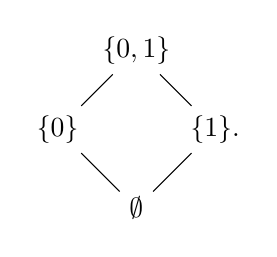
\begin{tikzpicture}
                \node (01) at (0, 0) {$\{0,1\}$};
                \node (0) at (-1, -1) {$\{0\}$};
                \node (1) at (1, -1) {$\{1\}.$};
                \node (empty) at (0, -2) {$\emptyset$};
                \draw (empty) -- (0) -- (01);
                \draw (empty) -- (1) -- (01);
            \end{tikzpicture}
        \end{gather*}
    \end{example}

    \newdef{Totally ordered set}{\index{totality}\label{set:total_order}
        A poset $P$ with the property that for all $x,y\in P$, either $x\leq y$ or $y\leq x$. This property is called \textbf{totality}.
    }
    \newdef{Strict total order}{
        A nonstrict order $\leq$ has an associated strict order $<$ that satisfies $x<y\iff x\leq y\land x\neq y$.
    }

    \newdef{Linear order}{
        A binary relation $<$ on a set $P$ satisfying the following conditions for all $x,y,z\in P$:
        \begin{enumerate}
            \item\textbf{Irreflexivity}: $x\not<x$,
            \item\textbf{Asymmetry}: $x<y\implies y\not<x$,
            \item\textbf{Transitivity}: $x<y\land y<z\implies x<z$,
            \item\textbf{Comparison}: $x<z\implies x<y\lor y<z$, and
            \item\textbf{Connectedness}: $x\not<y\land y\not<x\implies x=y$.
        \end{enumerate}
    }
    \remark{By negation, one can freely pass between linear orders and total orders. However, without the law of the excluded middle, there exists no bijection between them.}

    \newdef{Supremum}{\index{supremum}\label{set:supremum}
        The supremum $\sup(P)$ of a poset $P$ is the least upper bound of $P$.
    }
    \newdef{Infimum}{\index{infimum}\label{set:infimum}
        The infimum $\inf(P)$ of a poset $P$ is the greatest lower bound of $P$.
    }

    \newdef{Maximum}{\index{maximum}\label{set:maximum}
        If $\sup(P)\in P$, the supremum is called the maximum of $P$. This is denoted by $\max(P)$.
    }
    \newdef{Minimum}{\index{minimum}\label{set:minimum}
        If $\inf(P)\in P$, the supremum is called the minimum of $P$. This is denoted by $\min(P)$.
    }

    \newdef{Chain}{\index{chain}\label{set:chain}
        A totally ordered subset of a poset.
    }
    \begin{theorem}[Zorn's lemma\footnotemark]\index{Zorn's lemma}\label{set:zorns_lemma}
        \footnotetext{This theorem is equivalent to the \textit{axiom of choice}.}
        Let $(P,\leq)$ be a poset. If every chain in $P$ has an upper bound in $P$, then $P$ has a maximal element.
    \end{theorem}

    \newdef{Directed\footnotemark\ set}{\index{directed set}\index{filtered set|see{directed set}}\label{set:directed_set}
        \footnotetext{Sometimes called a \textbf{filtered} set or \textbf{upward} directed set. \textbf{Downward} directed sets are analogously defined with a lower bound for every two elements.}
        A set $P$ equipped with a preorder $\leq$ with the additional property that every 2-element subset has an upper bound, i.e.~for every two elements $x,y\in P$, there exists an element $z\in P$ such that $x\leq z\land y\leq z$.
    }
    \newdef{Net}{\index{net}\label{set:net}
        A net on a set $X$ is a subset of $X$ indexed by a directed set $I$.
    }

    \newdef{Cut}{\index{cut}\index{Dedekind!cut}\index{union!ordered}
        Let $(P,\leq)$ be a totally ordered set. A cut or \textbf{decomposition} of $P$ is a pair $(A,B)$ of disjoint subsets such that $P=A\cup B$ in the ordered sense, i.e.~every element of $A$ is smaller than every element of $B$. Cuts can be classified as follows:
        \begin{itemize}
            \item\textbf{Jumps}: $A$ has a greatest element and $B$ has a least element.
            \item\textbf{Dedekind cut}: Either $A$ has a greatest element and $B$ has no least element or $A$ has no greatest element, but $B$ has a least element.
            \item\textbf{Gap}: $A$ has no greatest element and $B$ has no least element.
        \end{itemize}
    }

    The notion of a filter on a set $X$ (\cref{set:filter}) is a specific example of a more general notion, where the underlying poset is the power set of $X$.
    \newdef{Filter}{\index{filter}\index{ultrafilter}\label{set:ultrafilter}
        Let $X$ be a poset. A filter on $X$ is a subset $\mathcal{F}\subseteq X$ such that:
        \begin{enumerate}
            \item\textbf{Nonemptiness}: $\mathcal{F}\neq\emptyset$,
            \item\textbf{Downward closure}: $\forall x,y\in\mathcal{F}:\exists z\in\mathcal{F}:z\leq x\land z\leq y$, and
            \item\textbf{Isotony}: If $x\in\mathcal{F}$ and $x\leq y$, then $y\in\mathcal{F}$.
        \end{enumerate}
        If there exists no strictly greater filter $\mathcal{F}\subset\mathcal{F}'$, then $\mathcal{F}$ is called an \textbf{ultrafilter}.
    }

    The following theorem is independent of the ZF axioms, but strictly weaker than the \textit{axiom of choice}.
    \begin{theorem}[Ultrafilter lemma]
        Every proper filter on a set is contained in an ultrafilter.
    \end{theorem}

\subsection{\difficult{Ordinals}}

    \newdef{Well-ordering}{\index{well-!order}\index{well-!founded}
        A \textbf{well-founded} linear order, i.e.~a linear order such that every nonempty subset has a minimal element.
    }

    \newdef{Ordinal number}{\index{number!ordinal}\label{set:ordinal}
        Consider the class of all well-ordered sets. An ordinal (type or rank) is an isomorphism class of well-ordered sets. The class of ordinals is itself well ordered by inclusion of `initial segments'.

        However, this definition gives problems within the ZF(C) framework of set theory, since these equivalence classes are proper classes and not sets. To overcome this problem, one can use a different approach. By using a well-defined construction, one can, for every class, select a particular representative and call this representative the \textbf{ordinal number} of all well-ordered sets isomorphic to it.
    }

    The most common construction is the one by \indexauthor{von Neumann}. For every well-ordered set $W$, there exists a function
    \begin{gather}
        W\rightarrow P(W):w\mapsto W_{\leq w}:=\{w'\in W\mid w'\leq w\}
    \end{gather}
    that restricts to an order isomorphism on its image. This leads to the following definition.
    \newdef{von Neumann ordinal}{\index{von Neumann!ordinal}
        A set that is strictly well ordered by membership and such that every element is also a subset.

        The first finite von Neumann ordinals are given as an example:
        \begin{itemize}
            \item $0 := \emptyset$,
            \item $1 := \{0\} = \{\emptyset\}$,
            \item $2 := \{0, 1\} = \{\emptyset,\{\emptyset\}\}$, and so on.
        \end{itemize}
    }

    \begin{property}
        Every ordinal type is uniquely order-isomorphic to an ordinal number. Consequently, every order-preserving isomorphism between an order type and itself is the identity.
    \end{property}

    \newdef{Successor}{\index{successor}\index{limit!ordinal|see{ordinal}}
        Every ordinal number $\alpha$ has a \textbf{successor} $\alpha^+$. Using the von Neumann definition, this is simply $\alpha^+ := \alpha\cup\{\alpha\}$. An ordinal that is not the successor of another ordinal number is called a \textbf{limit ordinal}.
    }
    \newdef{Regular ordinal}{\index{regular!ordinal}
        A limit ordinal $\alpha$ that is not the limit of a set of smaller ordinals with order type less than $\alpha$.
    }

    \begin{property}[Burali--Forti paradox]\index{Burali--Forti paradox}
        The class of all ordinals (and, by extension, the class of all well-ordered sets) is not a set.
    \end{property}

\subsection{\difficult{Cardinals}}

    There also exist numbers representing the sizes of sets, the \textbf{cardinal numbers}. These `numbers' should satisfy the following conditions:
    \begin{enumerate}
        \item Every set has a well-defined cardinality.
        \item Every cardinal number is the cardinality of some set.
        \item Bijective sets have the same cardinality.
    \end{enumerate}
    Guided by these conditions, one could naively use the following definition.
    \newdef{Cardinal number\footnotemark}{\index{number!cardinal}
        \footnotetext{Also called the \textbf{cardinality} of a set.}
        An isomorphism class of sets (under bijections).
    }

    However, similar to the problem encountered for ordinals above, these classes are not sets. To solve this, one can also use a similar trick and select a specific representative. For cardinals, the following choice is common.
    \newadef{Cardinal number}{
        The cardinal number of a set is the smallest ordinal rank of any well-order on it, i.e.~any ordinal number bijective to it.\footnote{The \textit{well-ordering theorem} (if assumed) assures that this definition coincides with the naive one above.} The cardinal numbers inherit a well-ordering from the ordinal numbers.
    }

    \begin{remark}[Ordering]
        The Cantor--Bernstein--Schr\"oder theorem~\ref{set:CBS_theorem} induces a partial ordering on cardinal numbers. However, without the axiom of choice this can never be a total ordering. This problem is also apparent in the above definition since the ordinal rank of sets is used together with the \textit{well-ordering theorem}, which is equivalent to the axiom of choice.
    \end{remark}

    Similar to ordinal numbers, one can also define successors of cardinal numbers.
    \newdef{Successor}{\index{successor}
        Given a cardinal $\kappa$, its successor $\kappa^+$ is defined as the smallest cardinal greater than $\kappa$.
    }
    \begin{remark}
        It should be noted that the successor of a cardinal number is not necessarily the same as its successor as an ordinal number (in fact, this is only the case for finite cardinals).
    \end{remark}

    \newdef{Regular cardinal}{\index{regular!cardinal}\label{set:regular_cardinal}
        An infinite cardinal $\kappa$ such that there exists no set of cardinality $\kappa$ that is the union of less than $\kappa$ subsets of cardinality less than $\kappa$:
        \begin{gather}
            \left(\kappa=\sum_{i\in I}\lambda_i\right)\land\bigl(\forall i\in I:\lambda_i<\kappa\bigr)\implies|I|\geq\kappa.
        \end{gather}
    }

    The following theorem can easily be proven by a diagonal argument.
    \begin{theorem}[Cantor]\index{Cantor}
        Let $S$ be a set of cardinality $\kappa$. The power set $P(S)$ has cardinality strictly greater than $\kappa$.
    \end{theorem}

\subsection{Lattices}

    \newdef{Semilattice}{\index{join}\index{meet}
        A poset $(P,\leq)$ for which every 2-element subset has a supremum, called the \textbf{join}, is called a \textbf{join-semilattice}. Similarly, a poset $(P,\leq)$ for which every 2-element subset has an infimum, called the \textbf{meet}, is called a \textbf{meet-semilattice}.
    }
    \begin{notation}
        The join of $\{x,y\}$ is denoted by $x\land y$. The meet of $\{x,y\}$ is denoted by $x\lor y$.
    \end{notation}
    \newdef{Lattice}{\index{lattice}
        A poset that is both a join- and a meet-semilattice.
    }

    The above definition also allows for a purely algebraic formulation (in this case, some authors might speak about \textbf{lattice-ordered sets}).
    \newadef{Lattice}{\index{absorption!law}\index{lattice}
        A lattice is an algebraic structure that admits operations $\land,\lor$ that satisfy the following conditions:
        \begin{enumerate}
            \item Both $\land$ and $\lor$ are idempotent, commutative and associative.
            \item The operations satisfy the \textbf{absorption laws}:
            \begin{gather}
                x\lor(x\land y)=x \qquad\qquad\qquad x\land(x\lor y)=x.
            \end{gather}
        \end{enumerate}
        To go from this definition to the order-theoretic one, define the partial order
        \begin{gather}
            x\leq y\iff x\land y=x\,.
        \end{gather}
        There exists an equivalent relation for the join.
    }

    \newdef{Complete lattice}{\index{complete!lattice}\index{adjoint functor theorem}\index{Dedekind!completeness}\label{set:complete_lattice}
        A lattice is said to be $\sigma$-complete (resp.~complete) if it admits all\footnote{When working with \textit{categories} (see \labelref{chapter:cat}), this has to be restricted to `all small joins/meets' or, equivalently, the index category should be a set.} countable (resp.~all) joins. It can be proven that complete lattices also admit all meets (as a special case of the \textit{Adjoint Functor Theorem}~\ref{cat:adjoint_functor_theorem}). If only bounded (from above) subsets admit a join, the lattice is said to be \textbf{Dedekind-complete}. 
    }

    \newdef{Bounded lattice}{\index{lattice!bounded}
        A lattice $(L,\leq,\land,\lor)$ that contains a greatest element (denoted by $\top$ or 1) and a smallest element (denoted by $\bot$ or 0) such that
        \begin{gather}
            \bot\leq x\leq\top
        \end{gather}
        for all $x\in P$. These elements are the identities for the join and meet operations:
        \begin{gather}
            x\land\top=x\qquad\qquad\qquad x\lor\bot=x\,.
        \end{gather}
    }

    \newdef{Frame}{\index{frame!set theory}\index{distributivity}\label{set:frame}
        A complete lattice $(L,\leq,\land,\lor)$ for which the \textbf{infinite distributivity law} is satisfied:
        \begin{gather}
            y\land\left(\bigvee_{i\in I}x_i\right) = \bigvee_{i\in I}\left(y\land x_i\right)\,.
        \end{gather}
    }

    \newdef{Distributive lattice}{\index{lattice!distributive}\index{modular|seealso{lattice}}\index{lattice!modular}
        A lattice $(L,\leq,\land,\lor)$ such that
        \begin{gather}
            a\land(b\lor c) = (a\land b)\lor(a\land c)
        \end{gather}
        and\footnote{This second condition is actually a consequence of the first.}
        \begin{gather}
            a\lor(b\land c) = (a\lor b)\land(a\lor c)
        \end{gather}
        for all $a,b,c\in L$. If only
        \begin{gather}
            a\leq c\implies a\lor(b\land c)=(a\lor b)\land c
        \end{gather}
        holds, the lattice is said to be \textbf{modular}.
    }
    \newdef{Complemented lattice}{\index{complement}\index{lattice!orthomodular}\label{set:complemented_lattice}
        A bounded lattice $(L,\leq,\land,\lor,\top,\bot)$ such that for every $a\in L$, there exists at least one $b\in L$ such that
        \begin{gather}
            a\land b=\bot \qquad\text{and}\qquad a\lor b=\top\,.
        \end{gather}
        If a consistent assignment of \textbf{(ortho)complements} exists, i.e.~for all $a,b\in L$:
        \begin{enumerate}
            \item\textbf{Involutivity}: $a^{\perp\perp}=a$, and
            \item\textbf{Order-reversing}: $a\leq b\iff b^\perp\leq a^\perp$,
        \end{enumerate}
        the lattice is said to admit an \textbf{orthocomplementation}. When, furthermore,
        \begin{gather}
            a\leq b\implies a\lor(a^\perp\land b)=b
        \end{gather}
        for all $a,b\in L$, then $L$ is said to be \textbf{orthomodular}. (Comparing to the previous definition, this shows that orthomodularity is an even weaker form of distributivity than modularity, where distributivity only holds with respect to complements.)
    }
    \begin{property}[de Morgan]
        All (ortho)complemented lattices satisfy de Morgan's laws~\eqref{set:de_morgan_union} and~\eqref{set:de_morgan_intersection}.
    \end{property}

    \newdef{Heyting algebra}{\index{Heyting!algebra}\index{pseudo-!complement}\label{set:heyting}
        A bounded lattice $(L,\leq,\land,\lor,\top,\bot)$ such that, for every two elements $a,b\in L$, there exists a greatest element $x\in L$ such that
        \begin{gather}
            a\wedge x\leq b\,.
        \end{gather}
        This element is denoted by $a\rightarrow b$. The \textbf{pseudocomplement} $\neg a$ of an element $a\in L$ is then defined as $a\rightarrow\bot$. Note that pseudocomplements do not define an orthocomplementation since
        \begin{gather}
            a\lor a^\perp=\top
        \end{gather}
        does not have to hold.
    }
    \newdef{Boolean algebra}{\index{law!of excluded middle}\index{Boolean!algebra}\label{set:boolean}
        A Heyting algebra $L$ in which the \textbf{law of excluded middle} holds:
        \begin{gather}
            \forall a\in L:\neg\neg a=a\,.
        \end{gather}
        This can be equivalently stated as
        \begin{gather}
            \forall a\in L:a\lor\neg a=\top\,.
        \end{gather}
        This is equivalent to a complemented, distributive lattice.
    }

\section{Limits}

    \newdef{Direct system}{\index{direct!system}
        Let $(I,\leq)$ be a directed set (\cref{set:directed_set}) and let $(A_i)_{i\in I}$ be a family of objects. Consider a family of morphisms $(f_{ij}:A_i\rightarrow A_j)_{i,j\in I}$ between these objects with the following properties:
        \begin{enumerate}
            \item for every $i\in I$: $f_{ii} = \mathbbm{1}_{A_i}$, and
            \item for every $i\leq j\leq k\in I$: $f_{ik} = f_{jk}\circ f_{ij}$.
        \end{enumerate}
        The pair $(A_i,f_{ij})$ is called a direct system (over $I$).
    }

    \newdef{Direct limit}{\index{direct!limit}\index{inductive!limit}\label{set:direct_limit}
        Consider a direct system $(A_i,f_{ij})$ over a directed set $I$. The direct (or \textbf{inductive}) limit $A$ of this direct system is defined as follows:
        \begin{gather}
            \varinjlim A_i := \bigsqcup_{i\in I}A_i\Big/\!\sim\,,
        \end{gather}
        where the equivalence relation is given by
        \begin{gather}
            x\in A_i\sim y\in A_j\iff\exists k\in I: f_{ik}(x) = f_{jk}(y)\,.
        \end{gather}
        Informally put: two elements are equivalent if they eventually become the same. The operations on $A$ are defined such that the inclusion maps $\phi_i:A_i\rightarrow A$ are morphisms.
    }

    \newdef{Inverse system}{\index{inverse!system}
        Let $(I,\leq)$ be a directed set (\cref{set:directed_set}) and let $(A_i)_{i\in I}$ be a family of objects. Consider a family of morphisms $(f_{ij}:A_j\rightarrow A_i)_{i,j\in I}$ between these objects with the following properties:
        \begin{enumerate}
            \item for every $i\in I$: $f_{ii} = \mathbbm{1}_{A_i}$, and
            \item for every $i\leq j\leq k\in I$: $f_{ik} = f_{ij}\circ f_{jk}$.
        \end{enumerate}
        The pair $(A_i,f_{ij})$ is called an inverse system (over $I$).
    }

    \newdef{Inverse limit}{\index{inverse!limit}\index{projective!limit}\label{set:inverse_limit}
        Consider an inverse system $(A_i,f_{ij})$ over a directed set $I$. The inverse (or \textbf{projective}) limit $A$ of this inverse system is defined as follows:
        \begin{gather}
            \varprojlim A_i := \left\{\vec{a}\in\prod_{i\in I}A_i\,\middle\vert\,a_i=f_{ij}(a_j), \forall i\leq j\right\}\,.
        \end{gather}
        For all $k\in I$, there exists a natural projection $\pi_k:\varprojlim A_i\rightarrow A_k$.
    }

    \begin{remark}
        The direct and inverse limit are each other's (\textit{categorical}) dual. The former is a \textit{colimit} while the latter is a \textit{limit} in category theory. (See \cref{section:diagrams}.)
    \end{remark}

\section{Partitions}
\subsection{Partition}\label{section:partition}

    \newdef{Composition}{\index{composition}
        Let $k,n\in\mathbb{N}$. A $k$-composition of $n$ is a $k$-tuple $(t_1,\ldots, t_k)\subset\mathbb{N}$ such that $\sum_{i=1}^kt_k = n$.
    }
    \newdef{Partition}{\index{partition}
        Let $n\in\mathbb{N}$. A partition of $n$ is an ordered composition of $n$ (usually in decreasing order). Hence multiple different composition can determine the same partition.
    }

    \newdef{Young diagram\footnotemark}{\index{Young!diagram}\index{Ferrers diagram|see{Young diagram}}
        \footnotetext{Sometimes called a \textbf{Ferrers diagram}.}
        A Young diagram is a visual representation of the partition of an integer $n$. It is a left justified system of boxes, where every row corresponds to an element of the partition:
        \begin{figure}[!ht]
            \centering
            \ydiagram{5, 4, 4, 1}
            \caption{A Young diagram representing the partition $(5,4,4,1)$ of 14.}
            \label{fig:young_diagram}
        \end{figure}
    }
    \newdef{Conjugate partition}{
        Let $\lambda$ be a partition of $n$ with associated Young diagram $\mathcal{D}$. The conjugate partition $\lambda'$ is obtained by reflecting $\mathcal{D}$ across the main diagonal. Since the number of boxes is left invariant, conjugate partitions are partitions for the same integer.
    }
    \begin{example}
        Conjugating Diagram~\ref{fig:young_diagram} gives Diagram~\ref{fig:young_diagram_conj} below. The associated partition is $(4,3,3,3,1)$.
        \begin{figure}[!ht]
            \centering
            \ydiagram{4, 3, 3, 3, 1}
            \caption{A Young diagram representing the partition $(4,3,3,3,1)$ of 14.}
            \label{fig:young_diagram_conj}
        \end{figure}
    \end{example}

    \newdef{Young tableau}{\index{Young!tableau}
        Consider a Young diagram of shape $\lambda$. A Young tableau of shape $\lambda$ is a filling of the corresponding Young diagram by the elements of a totally ordered set (with $n$ elements). This tableau is said to be \textbf{standard} if every row and every column is increasing.
    }

    \begin{formula}[Hook length formula]\index{hook length}
        The \textbf{hook} $H_{i,j}$ is defined as the part of a Young diagram given by the cell $(i,j)$ together with all cells below and to the right of $(i,j)$. Given a hook $H_{i,j}$, define the \textbf{hook length} $h_{i,j}$ as the cardinality of $H_{i,j}$.

        The number $f^\lambda\in\mathbb{N}$ of possible standard Young tableaux of shape $\lambda$, where $\lambda$ defines a partition of $n$, is given by the following formula:
        \begin{gather}
            f^\lambda = \frac{n!}{\prod_{(i,j)\in\lambda}h_{i,j}}\,.
        \end{gather}
    \end{formula}

    \newdef{Young tabloid}{
        A Young tabloid of shape $\lambda$ is defined as an equivalence class of Young tableaux that are related by permuting the elements within a row. These are often drawn as in \cref{fig:young_tabloid}. Note that every Young tabloid is represented by exactly one Young tableau.
        \begin{figure}[!ht]
            \centering
            \ytableausetup{boxsize=normal,tabloids}
                \begin{ytableau}
                    1&2&3&5&8\\
                    4&6&9&10\\
                    7&11&12&14\\
                    15
                \end{ytableau}
            \caption{A Young tabloid associated to the Young diagram in Figure \ref{fig:young_diagram}.}
            \label{fig:young_tabloid}
        \end{figure}
    }

\subsection{\difficult{Superpartition}}

    For the physical background of the notions introduced in this section, see \cref{section:mathematical_formalism_qm}.

    \newdef{Superpartition}{\index{partition}\index{fermion}\index{degree!of superpartition}
        Let $m,n\in\mathbb{N}$. A superpartition in the $m$-\textbf{fermion sector} is a sequence of integers of the following form:
        \begin{gather}
            \Lambda = (\Lambda_1,\ldots,\Lambda_m;\Lambda_{m+1},\ldots,\Lambda_n)\,,
        \end{gather}
        where the first $m$ numbers are strictly ordered, i.e.~$\Lambda_i>\Lambda_{i+1}$ for all $i<m$, and the last $n-m$ numbers form a normal partition.

        Both sequences, separated by a semicolon, form in fact distinct partitions themselves. The first one represents the \textbf{antisymmetric, fermionic sector} (this explains the strict order) and the second one represents the \textbf{symmetric, bosonic sector}. This amounts to the following notation:
        \begin{gather*}
            \Lambda\equiv(\lambda^a;\lambda^s)\,.
        \end{gather*}
        The \textbf{degree} of the superpartition is given by $|\Lambda|:=\sum_{i=1}^n\Lambda_i$.
    }
    \begin{notation}
        A superpartition of degree $n\in\mathbb{N}$ in the $m$-fermion sector is said to be a superpartition of $(n|m)$. To every superpartition $\Lambda$, one can also associate a unique partition $\Lambda^*$ by removing the semicolon and reordering the numbers such that they form a partition of $n$. The superpartition $\Lambda$ can then be represented by the Young diagram belonging to $\Lambda^*$, where the rows belonging to the fermionic sector are terminated by a circle.
    \end{notation}
% \chapter{Algebra}

    For the later sections on (co)homology theory some terminology from Chapter \ref{chapter:hom_alg} is used.

\section{Algebraic structures}

    \newdef{Semigroup}{\index{semi-!group}\index{magma}\label{algebra:semigroup}
        A set $G$ equipped with a binary operation $\star$ such that the following axioms are satisfied:
        \begin{enumerate}
            \item\textbf{Closure}: $G$ is closed under $\star$.
            \item\textbf{Associativity}: $\star$ is asssociative.
        \end{enumerate}
        If the associativity axiom is dropped, a \textbf{magma} is obtained.
    }

    \newdef{Monoid}{\index{monoid}\label{algebra:monoid}
        A set $M$ equipped with a binary operation $\star$ such that the following axioms are satisfied:
        \begin{enumerate}
            \item\textbf{Closure}: $M$ is closed under $\star$.
            \item\textbf{Associativity}: $\star$ is associative.
            \item\textbf{Unitality}: $M$ contains an identity element with respect to $\star$.
        \end{enumerate}
    }
    \newdef{Nilpotent}{\index{nilpotent}\label{algebra:nilpotent}
        An element $x$ of a monoid for which there exists an integer $k\in\mathbb{N}$ such that $x^k=e$, where $e$ is the identity element.
    }
    \begin{property}[Eckmann-Hilton argument]\index{Eckmann-Hilton!argument}\label{algebra:eckmann_hilton}
        Let $(M,\circ),(M,\otimes)$ be two monoid structures (or even unital magma structures) on a set $M$ such that
        \begin{gather}
            (a\circ b)\otimes(c\circ d) = (a\otimes c)\circ(b\otimes d)
        \end{gather}
        for all $a,b,c,d\in M$. The two monoid structures coincide and are in fact Abelian. (This property admits a vast generalization, see \ref{cat:eckmann_hilton}.)
    \end{property}

    \newdef{Group}{\index{group}
        \nomenclature[S_Grp]{$\textbf{Grp}$}{category of groups and group homomorphisms}
        A set $G$ equipped with a binary operation $\star$ such that the following axioms are satisfied:
        \begin{enumerate}
            \item\textbf{Closure}: $G$ is closed under $\star$.
            \item\textbf{Associativity}: $\star$ is asssociative.
            \item\textbf{Unitality}: $G$ has an identity element with respect to $\star$.
            \item\textbf{Inverses}: Every element in $G$ has an inverse with respect to $\star$.
        \end{enumerate}
    }
    \newnot{Identity element}{
        The identity element of a general group will be denoted by $e$. In certain cases, where this makes sense, the identity element will be denoted by 0 or 1 (additive and multiplicative conventions).
    }
    \newdef{Abelian group}{\index{commutativity}\index{Abelian group}
        \nomenclature[S_Ab]{$\text{Ab}$}{category of Abelian groups}
        Let $(G,\star)$ be a group. If $\star$ is commutative, then $G$ is said to be an Abelian or \textbf{commutative} group.
    }

    \newdef{Morphism}{\index{morphism!of groups}
        A group \textbf{(homo)morphism} $\Phi:(G,\star)\rightarrow(H,\cdot)$ is a function $f:G\rightarrow H$ such that
        \begin{gather}
            \Phi(g\star g') = \Phi(g)\cdot\Phi(g')
        \end{gather}
        for all $g,g'\in G$.
    }

    \newdef{Kernel}{\index{kernel}\label{group:kernel}
        The kernel of a group morphism $\Phi:G\rightarrow H$ is defined as the set
        \begin{gather}
            \ker(\Phi) := \{g\in G\mid\Phi(g)=e_H\}.
        \end{gather}
        This set carries a group structure induced by that on $G$.
    }

    \begin{theorem}[First isomorphism theorem]\index{isomorphism theorem}\label{group:first_isomorphism_theorem}
        Consider a group morphism $\Phi:G\rightarrow H$. If $\Phi$ is surjective, then $G/\ker(\Phi)\cong H$.
    \end{theorem}

\section{Group theory}\label{section:groups}

    \newdef{Order of a group}{\index{order!of a group}
        The number of elements in the group. It is denoted by $|G|$ or $\mathrm{ord}(G)$.
    }
    \newdef{Order of an element}{
        The order of an element $a\in G$ is the smallest integer $n\in\mathbb{N}$ such that
        \begin{gather}
            a^n = e,
        \end{gather}
        where $e$ is the identity element of $G$.
    }

    \newdef{Torsion group}{\index{torsion!group}\label{group:torsion_group}
        A group in which all elements have finite order. The torsion set $\mathrm{Tor}(G)$ of a group $G$ is the set of all elements $a\in G$ that have finite order. If $G$ is Abelian, $\mathrm{Tor}(G)$ is a subgroup.
    }

    \begin{theorem}[Lagrange]\index{Lagrange}
        Let $G$ be a finite group and let $H$ be a subgroup. Then $|H|$ is a divisor of $|G|$.
    \end{theorem}
    \begin{result}
        The order of any element $g\in G$ is a divisor of $|G|$.
    \end{result}

    \begin{construct}[Grothendieck completion]\index{Grothendieck!completion}\label{group:grothendieck_completion}
        Let $(A,\boxplus)$ be a commutative monoid. From this monoid one can construct an Abelian group $G(A)$, called the Grothendieck completion of $A$, as the quotient of $A\times A$ by the equivalence relation
        \begin{gather}
            (a_1,a'_1)\sim (a_2,a'_2) \iff\exists c\in A: a_1 \boxplus a'_2 \boxplus c = a'_1 \boxplus a_2 \boxplus c.
        \end{gather}
        The identity element, denoted by 0, is given by the equivalence class of $(0,0)$. By the definition of $G(A)$, this class contains all elements $\alpha\in\Delta_A$. In particular, $[(a,b)]$ is the additive inverse of $[(b,a)]$: $[(a,b)] + [(b,a)] = 0$.
    \end{construct}
    \begin{uproperty}
        Let $G(A)$ be the Grothendieck completion of $A$. Every monoid morphism $m:A\rightarrow B$, between an Abelian monoid and an Abelian group, factors uniquely through a group morphism $\varphi:G(A)\rightarrow B$.
    \end{uproperty}

    \begin{example}[Integers]
        The Grothendieck completion of the natural numbers is the additive group of integers $\mathbb{Z}$.
    \end{example}

\subsection{Cosets}\index{co-!set}

    \newdef{Coset}{\index{normal!subgroup}\index{invariant!subgroup|see{normal subgroup}}\label{group:coset}
        Let $G$ be a group and let $H$ be a subgroup. The left coset of $H$ with respect to $g\in G$ is defined as the set
        \begin{gather}
            gH := \{gh\mid h\in H\}.
        \end{gather}
        The right coset is defined analogously. If for all $g\in G$ the left and right cosets coincide, the subgroup $H$ is said to be a \textbf{normal subgroup}, \textbf{normal divisor} or \textbf{invariant subgroup}.
    }
    \begin{notation}
        The set of left (resp. right) cosets is denoted by $G/H$ (resp. $H\backslash G$).
    \end{notation}

    \newdef{Index}{\index{index!of a subgroup}\label{group:index}
        Consider a group $G$ and a subgroup $H$. The index $|G:H|$ of $H$ in $G$ is defined as the number of cosets oh $H$ in $G$. This can also be expressed as
        \begin{gather}
            |G| = |G:H||H|.
        \end{gather}
    }

    \newadef{Normal subgroup}{\index{normal!subgroup}\index{conjugacy class}\label{group:normal_subgroup}
        Let $G$ be a group and let $H$ be a subgroup. Consider the \textbf{conjugacy classes} $gHg^{-1}$ for all $g\in G$. If all classes coincide with $H$ itself, then $H$ is said to be a normal subgroup.
    }
    \begin{notation}
        If $N$ is a normal subgroup of $G$, this is often denoted by $N\vartriangleleft G$.
    \end{notation}

    \newdef{Quotient group}{\index{quotient!group}\label{group:quotient_group}
        Let $G$ be a group and let $N\vartriangleleft$ be a normal subgroup. The coset space $G/N$ can be turned into a group by equipping it with the product induced by that on $G$.
    }

    \newdef{Center}{\index{center}\label{group:center}
        The center of a group $G$ is defined as follows:
        \begin{gather}
            Z(G) := \{z\in G\mid\forall g\in G:zg = gz\}.
        \end{gather}
        This is a normal subgroup of $G$.
    }
    \newdef{Normalizer}{\index{normalizer}
        The normalizer of a subgroup $H\subset G$ is defined as follows:
        \begin{gather}
            N_G(H) := \{g\in G\mid\forall gHg^{-1}=H\}\equiv\{g\in G\mid[G,H]\subseteq H\}.
        \end{gather}
    }
    \newdef{Centralizer}{\index{centralizer}
        The centralizer of a subgroup $H\subset G$ is defined as follows:
        \begin{gather}
            C_G(H) := \{g\in G\mid\forall h\in H:ghg^{-1}=h\}\equiv\{g\in G\mid[G,H]=0\}.
        \end{gather}
        This group clearly satisfies $C_G(H)\triangleleft N_G(H)$.
    }

\subsection{Sylow theorems}\index{Sylow}

    \newdef{Sylow $p$-subgroup}{\index{Sylow!subgroup}
        \nomenclature[S_Syl]{$\mathrm{Syl}_p(G)$}{set of Sylow $p$-subgroups of a finite group $G$}
        Consider a finite group $G$. For every prime $p$, a Sylow $p$-subgroup of $G$ is defined as a maximal $p$-group in $G$, i.e.~every element has order a power of $p$ and the subgroup is maximal with resect to this property. The set of all Sylow $p$-subgroups of $G$ is denoted by $\mathrm{Syl}_p(G)$.
    }

    \begin{theorem}[Sylow I]
        Consider a finite group $G$. For every prime factor $p$ of $|G|$ with multiplicity $n$, there exists a Sylow $p$-subgroup of order $p^n$.
    \end{theorem}
    \begin{theorem}[Sylow II]
        Consider a finite group $G$ and a prime factor $p$ of $|G|$. All Sylow $p$-subgroups are conjugate and, in particular, isomorphic.
    \end{theorem}
    \begin{theorem}[Sylow III]
        Consider a finite group $G$ together with a prime factor $p$ of $|G|$ of multiplicity $n$ such that $|G|=p^nm$ for some $m\in\mathbb{N}$ and write $n_p:=\mathrm{card}(\mathrm{Syl}_p(G))$.
        \begin{itemize}
            \item $m=|G:H|$ for every Sylow $p$-subgroup $H$ of $G$.
            \item $n_p|m$, i.e.~$n_p$ divides $m$.
            \item $n_p=1\bmod p$.
            \item $n_p=|G:N_G(H)|$ for any Sylow $p$-subgroup $H$ of $G$.
        \end{itemize}
    \end{theorem}

\subsection{Abelian groups}

    \newdef{Commutator subgroup\footnotemark}{\index{commutator!subgroup}\index{derived!subgroup}
        \footnotetext{Also called the \textbf{derived subgroup}.}
        The commutator subgroup $[G,G]$ of $G$ is defined as the group generated by the \textbf{commutators} \[[g,h] := g^{-1}h^{-1}gh,\] where $g,h\in G$. This group is a normal subgroup of $G$.
    }

    \begin{property}[Abelianization]\index{Abelianization}
        The Abelianization $G/[G,G]$ is an Abelian group. A group $G$ is Abelian if and only if $[G,G]$ is trivial.
    \end{property}

    \begin{property}[Abelian quotients]
        A quotient group $G/H$ is Abelian if and only if $[G,G]\leq H$.
    \end{property}


\subsection{Symmetric groups}

    \newdef{Symmetric group}{\index{symmetric!group}\index{degree!of symmetric group}\label{group:permutation_group}
        \nomenclature[S_symgr]{$S_n$}{symmetric group of degree $n$}
        \nomenclature[S_symgrX]{$\Sym(X)$}{symmetric group on the set $X$}
        The symmetric group $S_n$ (on $n$ elements) is defined as the set of all permutations of $\{1,\ldots,n\}$. The number $n$ is called the \textbf{degree} of the symmetric group. The symmetric group $\Sym(X)$ on a finite set $X$ is defined similarly (by first numbering the elements and then acting by $S_n$)\footnote{Two such choices are related through conjugation by a unique permutation. The resulting groups are isomorphic.}.

        When including infinite sets the symmetric group $\Sym(X)$ is defined as the group of all bijections from $X$ to itself (the multiplication is given by function composition).
    }

    \begin{theorem}[Cayley]\index{Cayley}
        Every group is isomorphic to a subgroup of the permutation group $\Sym(G)$.
    \end{theorem}

    \newdef{Cycle}{\index{cycle}
        A $k$-cycle is a permutation of the form $(a_1\ a_2\ \ldots\ a_k)$ sending $a_i$ to $a_{i+1}$ (and $a_k$ to $a_1$). A \textbf{cycle decomposition} of an arbitrary permutation is the decomposition into a product of disjoint cycles.
    }
    \begin{property}[Cycles are cyclic]
        Let $\tau$ be a $k$-cycle. Then $\tau$ is $k$-cyclic (hence the name):
        \begin{gather}
            \tau^k = e.
        \end{gather}
    \end{property}
    \begin{example}
        Consider the set $\{1,2,3,4,5,6\}$. The permutation $\sigma:x\mapsto x+2\bmod6$ can be decomposed as $\sigma = (1\ 3\ 5)(2\ 4\ 6)$.
    \end{example}

    \newdef{Transposition}{\index{transposition}
        A permutation that exchanges two elements but leaves the other ones unchanged.
    }
    \begin{property}[Decomposition]
        Any permutation can be decomposed as a product of transpositions. A permutation is said to be \textbf{even} (resp. \textbf{odd}) if the number of transpositions in its decomposition is even (resp. odd). One can prove that the parity of a permutation is well-defined, i.e.~it is independent of the choice of decomposition.
    \end{property}

    \newdef{Alternating group}{\index{group!alternating}
        The alternating group $A_n$ is the subgroup of $S_n$ containing all even permutations, i.e.~those permutations that can be decomposed as an even number of transpositions.
    }

    \newdef{Shuffle}{\index{shuffle}\label{group:shuffle}
        A permutation $\sigma\in S_n$ is called a $(p,q)$-shuffle (where $p+q=n$) if there exist disjoint increasing sequences $I=\{i_1<\ldots<i_p\}$ and $J=\{j_1<\ldots<j_q\}$ such that
        \begin{gather}
            \sigma(x) =
            \begin{cases}
                k&x=i_k\\
                k+p&x=j_k.
            \end{cases}
        \end{gather}
        The name stems from the idea of dividing a deck of cards into two piles and interleaving them. This way the order in each pile is strictly preserved.

        An unshuffle $\tau\in S_n$ is defined as a permuation such that $\tau^{-1}$ is a shuffle, i.e.~there exist disjoint increasing sequences $I=\{i_1<\ldots<i_p\}$ and $J=\{j_1<\ldots<j_q\}$ such
        \begin{gather}
            \tau(k) =
            \begin{cases}
                i_k&k\leq p\\
                j_{k-p}&k>p.
            \end{cases}
        \end{gather}
    }

\subsection{Group presentations}

    \newdef{Generator}{\index{generator}
        A set of elements $\{g_i\}_{i\in I}\subset G$ (where $I$ can be infinite) is said to generate $G$ if every element in $G$ can be written as a product of the elements $g_i$. These elements are then called generators of $G$.
    }

    \newdef{Relations}{\index{relation}
        Let $G$ be a group. If the product of a number of elements $g\in G$ is equal to the identity $e$, this product is said to be a relation on $G$.
    }
    \newdef{Complete set of relations}{
        Let $G$ be a group generated by a set of elements $S$ (note that this set does not have be a group itself) and let $R$ be a set of relations on $S$. If $G$ is uniquely (up to an isomorphism) determined by $S$ and $R$, the set of relations is said to be complete.
    }

    \newdef{Presentation}{\index{presentation}\label{group:presentation}
        Let $G$ be a group with generators $S$ and let $R$ be a complete set of relations. The pair $(S,R)$ is called a presentation of $G$.

        If $R$ is finite, $G$ is said to be \textbf{finitely related}, while if $S$ is finite, $G$ is said to be \textbf{finitely generated}. If both $S$ and $R$ are finite, $G$ is said to be \textbf{finitely presented}.

        It is clear that every group can have many different presentations and that it is (very) difficult to tell if two groups are isomorphic by just looking at their presentations.
    }
    \begin{notation}
        The presentation of a group $G$ is often denoted by $\langle S|R \rangle$, where $S$ is the set of generators and $R$ the set of relations.
    \end{notation}

\subsection{Direct products}

    \newdef{Direct product}{\index{direct product!of groups}\label{group:direct_product}
        Let $G,H$ be two groups. The direct product $G\times H$ is defined as the set-theoretic Cartesian product $G\times H$ equipped with a group operation $\cdot$ defined as
        \begin{gather}
            (g_1,h_1)\cdot(g_2,h_2) = (g_1g_2,h_1h_2),
        \end{gather}
        where the operations on the right-hand side are the group operations in $G$ and $H$. This definition can be generalized to any number of groups, even an infinite number of them if one the $n$-tuples are replaced by elements of the infinite Cartesian product

        If $g\in G_1\times\cdots\times G_n$ can be written as $(g_1,\ldots,g_n)$ for $g_i\in G_i$, the $g_i$ are called the \textbf{components} of $g$.
    }

    \newdef{Weak direct product}{\index{direct sum!of groups}
        Consider the direct product of groups. The subgroup consisting of all elements for which all components, except finitely many of them, are the identity, is called the weak direct product. In the case of Abelian groups this is often called the \textbf{direct sum}. For a finite number of groups, the direct product and direct sum coincide.
    }
    \begin{notation}
        The direct sum is often denoted by $\oplus$ (in accordance with the notation for vector spaces and other algebraic structures that will be introduced further on).
    \end{notation}

    \newdef{Inner semidirect product}{\index{semi-!direct product}\index{split!product}
        Let $G$ be a group, $H\leq G$ a subgroup and $N\vartriangleleft G$ a normal subgroup. $G$ is said to be the inner semidirect product of $H$ and $N$, denoted by $N\rtimes H$, if it satifies the following equivalent statements:
        \begin{itemize}
            \item $G = NH := \{nh\mid n\in N,h\in H\}$, where $N\cap H = \{e\}$.
            \item For every $g\in G$ there exist a unique $n\in N,h\in H$ such that $g=nh$.
            \item For every $g\in G$ there exist a unique $n\in N,h\in H$ such that $g=hn$.
            \item There exists a group morphism $\rho:G\rightarrow H$ that satisfies $\rho|_H = e$ and $\ker(\rho)=N$.
            \item The composition of the natural embedding $i:H\rightarrow G$ and the projection $\pi:G\rightarrow G/N$ gives an isomorphism between $H$ and $G/N$.
        \end{itemize}
        Whenever $G$ is isomorphic to $N\rtimes H$, it is said to \textbf{split} over $N$.
    }
    \begin{property}[Normal subgroups]
        If both $H$ and $N$ in the above definition are normal, the inner semidirect product coincides with the direct product. In particular this includes the case of direct products. For a finite number of groups the direct product is generated by the elements of the groups.

        If the subgroups $H$ and $N$ have presentations $\langle S_H|R_H \rangle$ and $\langle S_N|R_N \rangle$, the direct product is given by
        \begin{gather}
            \label{group:direct_product_presentation}
            H\times N = \langle S_H\cup S_N|R_H\cup R_N \cup R_C \rangle,
        \end{gather}
        where $R_C$ is the set of relations that enforce the commutativity of $H$ and $N$.
    \end{property}

    \newdef{Outer semidirect product}{
        Let $G,H$ be two groups and let $\varphi:H\rightarrow\Aut(G)$ be a group morphism. The outer semidirect product $G\rtimes_\varphi H$ is defined as the set-theoretic Cartesian product $G\times H$ equipped with a binary relation $\cdot$ such that
        \begin{gather}
            (g_1,h_1)\cdot(g_2,h_2) = (g_1\varphi(h_1)(g_2),h_1h_2).
        \end{gather}
        The structure $(G\rtimes_\varphi H,\cdot)$ forms a group.

        By noting that the set $N=\{(g,e_H)\mid g\in G\}$ is a normal subgroup isomorphic to $G$, and that the set $B=\{(e_G,h)\mid h\in H\}$ is a subgroup isomorphic to $H$, one can also construct the outer semidirect product $G\rtimes_\varphi H$ as the inner semidirect product $N\rtimes B$.
    }

    \begin{remark}[Direct products]
        The direct product of groups is a special case of the outer semidirect product where the group morphism is given by the trivial map $\varphi:h\mapsto e_G$.
    \end{remark}

    Semidirect products can even be generalized further:
    \newdef{Bicrossed product of groups}{\index{bicrossed product}\index{matched pair}\label{group:bicrossed_product}
        Consider a group $G$ with two subgroups $K,H\leq G$ such that every element $g\in G$ can be uniquely decomposed as a product of an element in $K$ and an element in $H$. This implies that for $k\in K,h\in H$ there exists a unique decomposition of $kh$ of the form \[kh = (k\cdot h)k^h\] where $k\cdot h\in H$ and $k^h\in K$.

        It can be checked that the associativity of the product implies that $-\cdot-:K\times H\rightarrow H$ defines a left action of $K$ on $H$ and that $-^-:K\times H\rightarrow K$ defines a right action of $H$ on $K$. Some other properties are obtained in the same way:
        \begin{itemize}
            \item $e^h = e$,
            \item $k\cdot e = e$,
            \item $(kk')^h = k^{k'\cdot h}k'^h$, and
            \item $k\cdot(hh') = (k\cdot h)(k^h\cdot h')$.
        \end{itemize}
        Any two groups having this structure are said to form a \textbf{matched pair} (of groups). Given a matched pair of groups, one can define the bicrossed product $H \bowtie K$ as follows:
        \begin{gather}
            (h,k)(h',k') = \big(h(k\cdot h),k^{h'}k'\big).
        \end{gather}
    }

\subsection{Free groups}

    \newdef{Free group}{\index{free!group}\index{word}\label{group:free_group}
        Consider a set $S$. The free group on $S$ is the group generated by \textbf{words} in $S$, i.e.~finite sequences of elements in $S$.
    }
    The definition of a group presentation \ref{group:presentation} can now be restated:
    \newadef{Presentation}{\index{presentation}
        A group $G$ is said to have a presentation $\langle S|R \rangle$ if it is isomorphic to the quotient of the free group on $S$ by the normal subgroup generated by $R$.
    }

    \newdef{Free product}{
        Consider two groups $G,H$. The free product $G\ast H$ is defined as the set consisting of all words composed of elements in $G$ and $H$ together with the concatenation (and reduction\footnote{Two elements of the same group, written next to each other, are replaced by their product.}) as multiplication. Due to the reduction, every element in $G\ast H$ has a unique expression of the form $g_1h_1g_2h_2\cdots g_nh_n$.
    }
    \begin{remark}[Cardinality]
        For nontrivial groups the free product is always infinite.
    \end{remark}
    \newadef{Free product}{\index{free!product}
        The free product of two groups $G$ and $H$ can equivalently be defined as the free group on the set $G\cup H$. It follows that if $G,H$ have presentations $\langle S_G\mid R_G \rangle$ and $\langle S_H|R_H \rangle$ respectively, the free product is given by
        \begin{gather}
            G\ast H = \langle S_G\cup S_H|R_G\cup R_H \rangle.
        \end{gather}
        By comparing to \eqref{group:direct_product_presentation} it can be seen that the free product is a generalization of the direct product.
    }
    \newdef{Free product with amalgamation}{\index{amalgamation}
        Consider three groups $F,G,H$ together with two group morphisms $\phi:F\rightarrow G$ and $\psi:F\rightarrow H$. The free product with amalgamation $G\ast_F H$ is defined by adding the following set of relations to the presentation of the free product $G\ast H$:
        \begin{gather}
            \big\{\phi(f)\psi(f)^{-1} = e\,\big\vert\,f\in F\big\}.
        \end{gather}
        This is the same as saying that the free product with amalgamation can be constructed as
        \begin{gather}
            G\ast_F H = (G\ast H) / N_F,
        \end{gather}
        where $N_F$ is the normal subgroup generated by elements of the form $\phi(f)\psi(f)^{-1}$.
    }

    \newdef{Free Abelian group}{\index{basis}\index{rank!of a group}
        An Abelian group $G$ is said to be freely generated on the generators $\{g_i\}_{i\in I}$ if every element $g\in G$ can be uniquely written as a formal linear combination of the generators:
        \begin{gather}
            G = \left\{\sum_{i\in J}a_ig_i\,\middle\vert\,a_i\in\mathbb{Z}, J\subseteq I\text{ is finite}\right\}.
        \end{gather}
        The set of generators is called a \textbf{basis}\footnote{In analogy with the basis of a vector space.} of $G$. The number of elements in the basis is called the \textbf{rank} of $G$.
    }
    \begin{property}[Nielsen-Schreier]\index{Nielsen-Schreier}
        Every subgroup of a free group is free.
    \end{property}

    \begin{theorem}[Fundamental theorem of finitely generated groups]\index{fundamental theorem!of finitely generated groups}\index{torsion!group}\label{group:theorem:free_group}
        Every finitely generated Abelian group $G$ of rank $n$ can either be decomposed as a quotient of two free, finitely generated, Abelian groups
        \begin{gather}
            G = F/F'
        \end{gather}
        or as a direct sum of a free, finitely generated, Abelian group and a torsion group \ref{group:torsion_group}:
        \begin{gather}
            G = A\oplus T \qquad\text{with}\qquad T\equiv Z_{h_1}\oplus\cdots\oplus Z_{h_m}.
        \end{gather}
        In the second decomposition $A$ has rank $n-m$ and all $Z_{h_i}$ are cyclic groups of order $h_i$, where $h_i$ is the power a prime. The group $T$ is called the \textbf{torsion subgroup}.
    \end{theorem}
    \begin{property}[Uniqueness]
        The rank $n-m$ and the numbers $h_i$ from previous theorem are unique.
    \end{property}

\section{Group actions}\label{section:group_actions}

    \newdef{Group action}{\index{group!action}\label{group:group_action}
        Let $G$ be a group and let $X$ be a set. A map $\rho:G\times X \rightarrow X$ is called an action of $G$ on $X$ if it satisfies the following conditions for all $g,h\in G$ and $x\in X$:
        \begin{enumerate}
            \item \textbf{Identity}: $\rho(e,x) = x$.
            \item \textbf{Compatibility}: $\rho(gh,x) = \rho(g,\rho(h,x))$.
        \end{enumerate}
        The set $X$ is called a (left) \textbf{$G$-space} or \textbf{$G$-set}. Right $G$-spaces are defined a similar way.
    }
    \remark{Note that this definition already makes sense for monoids \ref{algebra:monoid}.}
    \begin{adefinition}\label{group:permutation_remark}
        A group action can equivalently be defined as a group morphism $\rho:G\rightarrow\Sym(X)$. It assigns a permutation of $X$ to every element $g\in G$. If the set $X$ is equipped with some extra algebraic structure, one should replace $\Sym(X)$ by $\Aut(X)$, i.e.~the action of $G$ should respect the structure.
    \end{adefinition}
    \begin{notation}
        The action $\rho(g,x)$ is often denoted by $g\cdot x$ or even $gx$ if no confusion can arise.
    \end{notation}

    \newdef{Equivariant map}{\index{equivariant!map}\index{morphism!of $G$-sets}\label{group:equivariant}
        Let $X,Y$ be two $G$-spaces. An equivariant map between these sets is a function $f:X\rightarrow Y$ satisfying
        \begin{gather}
            g\cdot f(x) = f(g\cdot x),
        \end{gather}
        where, by abuse of notation, the symbol $\cdot$ represents the group actions on both $X$ and $Y$. An equivariant map is sometimes called a \textbf{$G$-map}.\footnote{$G$-spaces together with the $G$-maps constitute a category.}
    }

    \begin{example}[$G$-module]\index{module!over a group}\index{intertwiner}\label{group:module}
        An Abelian group $M$ equipped with a left group action $\varphi:G\rightarrow\Aut(M)$, i.e.~an action that acts by group morphisms. Equivariant maps of $G$-modules are also called \textbf{intertwining maps} or \textbf{intertwiners}.
    \end{example}

    \newdef{Orbit}{\index{orbit}\label{group:orbit}
        The orbit of an element $x\in X$ with respect to the action a group $G$ is defined as the set
        \begin{gather}
            G\cdot x\equiv\{g\cdot x\mid g\in G\}.
        \end{gather}
        The relation \[p\sim q\iff\exists g\in G:p = g\cdot q\] induces an equivalence relation for which the equivalence classes coincide with the orbits of the $G$-action. The set of equivalence classes $X/\!\sim$, often denoted by $X/G$, is called the \textbf{orbit space}.
    }
    \newdef{Stabilizer}{\index{stabilizer}\index{iso-!tropy group}\index{little!group}
        The stabilizer group (also called \textbf{isotropy group} or \textbf{little group}) of an element $x\in X$ with respect to the action of a group $G$ is defined as the set
        \begin{gather}
            G_x := \{g\in G\mid g\cdot x = x\}.
        \end{gather}
        This is a subgroup of $G$ for all $x\in X$.
    }
    \begin{theorem}[Orbit-stabilizer theorem]
        Let $G$ be a group acting on a set $X$ and let $G_x$ be the stabilizer of some $x\in X$. The following relation holds:
        \begin{gather}
            |G\cdot x||G_x| = |G|.
        \end{gather}
    \end{theorem}

    \newdef{Free action}{\index{free}\label{group:free_action}
        A group action is said to be free if $g\cdot x=x$ implies $g=e$ for any $x\in X$. Equivalently, a group action is free if the stabilizer groups of all elements is trivial.
    }
    \newdef{Faithful action}{\index{faithful!action}\index{effective!action|see{faithful}}\label{group:faithful_action}
        A group action is said to be faithful or \textbf{effective} if the morphism $G\rightarrow\Aut(X)$ is injective. Alternatively, a group action is faithful if for every two group elements $g,h\in G$ there exists an element $x\in X$ such that $g\cdot x\neq h\cdot x$.
    }

    \newdef{Transitive action}{\index{transitive!action}\label{group:transitive}
        A group action is said to be transitive if for every two elements $x, y\in X$ there exists a group element $g\in G$ such that $g\cdot x = y$. Equivalently, a group action is transitive if there is only one orbit.
    }
    \begin{property}\label{group:transitive_action_property}
        Let $X$ be a set equipped with a transitive action of a group $G$. There exists a bijection $X\cong G/G_x$, where $G_x$ is the stabilizer of any element $x\in X$.\\
        \begin{proof}
            \begin{mdframed}[roundcorner=10pt, linecolor=blue, linewidth=1pt]
                Choose an element $x\in X$. The stabilizer of $x$ with respect to $G$ is the set \[S_x := \{g\in G\mid g\cdot x = x\}.\] Due to the transitivity of the group action one obtains that \[\forall x, y\in X: \exists h\in G: h\cdot x = y.\] So, for every $z\in X$ one can choose a group element $g_z$ such that $g_z\cdot x = z$. For all elements in the coset $g_zS_x = \{g_zs\in G\mid s\in S_x\}$ the following equality is satisfied: \[(g_zs)\cdot x = g_z\cdot (s\cdot x) = g_z\cdot x = z.\] This implies that the map $\Phi:G/S_x \rightarrow X$ is surjective.

                Now, one needs to prove that $\Phi$ is also injective. A proof by contradiction is given. Choose two distinct cosets $gS_x$ and $hS_x$. There exist two elements $G,H\in X$ such that $g\cdot x = G$ and $h\cdot x = H$. Assume that $G = H$. This means that
                \begin{align*}
                    &g\cdot x = h\cdot x\\
                    \iff&(h^{-1}g)\cdot x = x\\
                    \iff&h^{-1}g\in S_x\\
                    \iff&hS_x\ni h(h^{-1}g) = g.
                \end{align*}
                This would imply that $gS_x = hS_x$, which is in contradiction with the assumptions. It follows that $G\neq H$ and, hence, that $\Phi$ is injective.\qed
            \end{mdframed}
        \end{proof}
    \end{property}

    \newdef{Homogeneous space}{\index{homogeneous!space}
        A set equipped with a transitive group action.
    }
    \newdef{Principal homogenous space}{\index{torsor}\label{group:torsor}
        If the action of a group $G$ on a homogeneous space $X$ is also free, then $X$ is said to be a principal homogeneous space or \textbf{$G$-torsor}.
    }
    \begin{example}[Affine space]
        The $n$-dimensional affine space $\mathbb{A}^n$ is an $\mathbb{R}^n$-torsor.
    \end{example}

    \newdef{Crossed module}{\index{module!crossed}\index{Peiffer}\label{group:crossed_module}
        A crossed module is a quadruple $(G,H,t,\alpha)$ where:
        \begin{itemize}
            \item $G,H$ are two groups,
            \item $t$ is a group morphism $H\rightarrow G$, and
            \item $\alpha$ is a group morphism $G\rightarrow\Aut(H)$.
        \end{itemize}
        These data are required to satisfy two compatibility conditions:
        \begin{enumerate}
            \item\textbf{$G$-equivariance}:
            \begin{gather}
                t(\alpha(g)h) = gt(h)g^{-1}.
            \end{gather}
            \item\textbf{Peiffer identity}:
            \begin{gather}
                \alpha(t(h))h' = hh'h^{-1}.
            \end{gather}
        \end{enumerate}
    }

\section{Group cohomology}\index{cohomology!group}

    \newdef{Group cohomology}{\label{group:cohomology}
        Consider a group $G$ together with a $G$-module $A$. Define the $k^{th}$ \textbf{chain group} as
        \begin{gather}
            C^k(G;A) := \big\{\text{all set-theoretic functions from }G^k\text{ to }A\big\}.
        \end{gather}
        The coboundary map $d^k:C^k(G;A)\rightarrow C^{k+1}(G;A)$ is defined as follows:
        \begin{align}
            d^kf(g_1,\ldots,g_k,g_{k+1}) = g_1\cdot f(g_2,\ldots,&g_k,g_{k+1}) + (-1)^{k+1}f(g_1,\ldots,g_k)\nonumber\\ &+\sum_{i=1}^k(-1)^{i+1} f(g_1,\ldots,g_ig_{i+1},\ldots,g_k,g_{k+1}).
        \end{align}
        The cohomology groups are defined as the following quotient groups:
        \begin{gather}
            H^k(G;A) := \frac{\ker(d^k)}{\im(d^k)}.
        \end{gather}
    }

    ?? COMPLETE (ADD e.g. classification of extensions) ??

\section{Hochschild and cyclic cohomology}\index{cohomology!Hochschild}

    \newdef{Hochschild homology groups}{\label{algebra:hochschild_homology}
        Let $A$ be an associative algebra and consider an $A$-bimodule $M$. For all $n\geq0$ define
        \begin{gather}
            HC_n(A;M) := M\otimes A^{\otimes n}.
        \end{gather}
        The boundary operator $d:HC_n(A;M)\rightarrow HC_{n-1}(A;M)$ is defined as follows:
        \begin{align}
            d_n:m\otimes a_1\otimes\cdots\otimes a_n\mapsto ma_1\otimes\cdots\otimes a_n + \sum_{i=1}^{n-1}(-1)^im\otimes a_1&\otimes\cdots\otimes a_ia_{i+1}\otimes\cdots\otimes a_n\\
            &+ (-1)^na_1m\otimes\cdots\otimes a_n.\nonumber
        \end{align}
        The Hochschild homology is then given by the homology of this chain complex:
        \begin{gather}
            HH_\bullet(A;M) := \ker(d_n)/\im(d_{n+1}).
        \end{gather}
        This complex can be turned into a graded-commutative algebra by equipping it with the \textit{shuffle product}.
    }
    \begin{remark}[Cohomology]
        Hochschild cohomology of $A$ can be obtained by dualizing: $HC^n(A):=\hom(HC_n(A),K)$, where $K$ is the field over which $A$ is defined.
    \end{remark}

    \begin{theorem}[Hochschild-Kostant-Rosenberg]\index{Hochschild-Kostant-Rosenberg}
        Let $A=C^\infty(M)$ for $M$ a smooth manifold.
        \begin{gather}
            HH_\bullet(A)\cong\Omega^n(M).
        \end{gather}
    \end{theorem}

    \newdef{Cyclic homology}{\index{cohomology!cyclic}
        The cyclic chain complex $CC_\bullet(A)$ is the subcomplex of the Hochschild complex $HC_\bullet(A)$ obtained as the kernel of $1-\lambda$, where $\lambda$ is the permutation operator
        \begin{gather}
            \lambda:HC_n(A)\rightarrow HC_n(A):a_0\otimes\cdots\otimes a_n\mapsto(-1)^na_n\otimes a_0\otimes\cdots\otimes a_{n-1}.
        \end{gather}
        It can be shown that the Hochschild boundary operator commutes with the permutation operator and, hence, descends to the cyclic complex. The resulting homology is called cyclic homology $CH_\bullet(A)$. By dualizing one obtains cyclic cohomology.
    }

    \begin{example}[Smooth algebras]
        Consider the case of $A=C^\infty(M)$, where $M$ is a smooth manifold. Then
        \begin{gather}
            CH_n(A)\cong Z^n_\text{dR}(M)\oplus\bigoplus_{\substack{i=1\\n-2i\geq0}}H^{n-2i}_\text{dR}(M).
        \end{gather}
        For this reason cyclic cohomology will be used in noncommutative geometry to generalize de Rham cohomology.
    \end{example}

\section{Rings}\label{section:ring}

    \newdef{Ring}{\index{ring}
        Let $R$ be a set equipped with two binary operations $+,\cdot$ (called \textbf{addition} and \textbf{multiplication}). $(R,+,\cdot)$ is a ring if it satisfies the following axioms:
        \begin{enumerate}
            \item $(R,+)$ is an Abelian group.
            \item $(R,\cdot)$ is a monoid.
            \item Multiplication is distributive with respect to addition.
        \end{enumerate}
    }
    \newdef{Field}{\index{field}
        A ring $(R,+,\cdot)$ for which the monoid $(R\backslash\{1_+\},\cdot)$ is an Abelian group and $1_+\neq 1_\cdot$.
    }

    \newdef{Unit}{\index{unit}
        An invertible element of a ring $(R,+,\cdot)$. The set of units forms a group under multiplication.
    }

    \newdef{Integral domain}{\index{domain!integral}\label{algebra:integral_domain}
        A commutative ring $R$ in which the product of two nonzero elements is again nonzero.
    }

    \newdef{Reduced ring}{\index{ring!reduced}
        A ring that contains no nonzero nilpotents.
    }

    \begin{construct}[Localization]\index{localization}
        Let $R$ be a commutative ring and let $S$ be a multiplicatively closed set in $R$. Define an equivalence relation $\sim$ on $R\times S$ in the following way:
        \begin{gather}
            (r_1,s_1)\sim(r_2,s_2) \iff \exists t\in S:t(r_1s_2 - r_2s_1) = 0.
        \end{gather}
        The set $S^{-1}R:=(R\times S)/\sim$, called the localization of $R$ with respect to $S$, can now be turned into a ring by defining an addition and a multiplication. By writing $(r,s)\in S^{-1}R$ as the formal fraction $\frac{r}{s}$, these operations are defined in analogy with the those of ordinary fractions:
        \begin{itemize}
            \item\textbf{Addition}: $\displaystyle\frac{r_1}{s_1} + \frac{r_2}{s_2} = \frac{r_1s_2 + r_2s_1}{s_1s_2}$,
            \item\textbf{Multiplication}: $\displaystyle\frac{r_1}{s_1}\cdot\frac{r_2}{s_2} = \frac{r_1r_2}{s_1s_2}$.
        \end{itemize}
    \end{construct}
    \remark{The localization of $R$ with respect to the set $S$ can be interpreted as the ring obtained by collapsing $S$ into a single unit of $R$.}

    \begin{notation}\label{algebra:localization_notation}
        For specific cases different notations are sometimes used. For example, choose an element $f\in R$ and let $R_f$ denote the localization of $R$ with respect to the set of powers of $f$, i.e.~$S=\{f^n\mid n\in\mathbb{N}\}$. This is called the \textbf{localization at (the element)} $f$. Another example occurs when working with prime ideals. Let $P$ be a prime ideal (see the next section). It is not hard to show that the complement $R\backslash P$ is multiplicatively closed. The localization of $R$ with respect to this set is denoted by $R_P$ and is called the \textbf{localization at (the prime ideal)} $P$.
    \end{notation}

    \newdef{Valuation}{\index{valuation}
        Let $k$ be a field and let $\Gamma$ be a totally ordered\footnote{Definition \ref{set:total_order}.}, Abelian group. The group law and the order relation on $\Gamma$ can be extended to the union $\Gamma\cup\{\infty\}$ in the following way (the notation $\infty$ is only a convention):
        \begin{itemize}
            \item $g+\infty:=\infty+g:=\infty$ for all $g\in\Gamma$, and
            \item $g\leq\infty$ for all $g\in\Gamma$.
        \end{itemize}
        A valuation on $k$ (with values in $\Gamma$) is a map $\nu:k\rightarrow\Gamma\cup\{\infty\}$ such that:
        \begin{enumerate}
            \item $\nu(a) = \infty\iff a = 0$;
            \item $\nu(ab) = \nu(a) + \nu(b)$; and
            \item $\min(\nu(a),\nu(b))\leq\nu(a+b)$, where the equality holds if $\nu(a)\neq\nu(b)$.
        \end{enumerate}
    }

\subsection{Ideals}

    \newdef{Ideal}{\index{ideal}\label{algebra:ideal}
        Let $(R,+,\cdot)$ be a ring with $(R,+)$ its additive group. A subset $I\subseteq R$ is called a (two-sided) ideal of $R$ if it satisfies the following conditions:
        \begin{enumerate}
            \item $(I,+)$ is a subgroup of $(R,+)$.
            \item $\forall n\in I,\forall r\in R:n\cdot r,r\cdot n\in I$.
        \end{enumerate}
    }

    \newdef{Artinian ring}{\index{Artin!ring}
        A ring is said to be Artin(ian) if it satisfies the \textbf{descending chain condition} on ideals, i.e.~if it contains no infinite descending chain \ref{set:chain} of ideals.
    }
    \newdef{Noetherian ring}{\index{Noether!ring}
        A ring is said to be Noether(ian) if it satisfies the \textbf{ascending chain condition} on ideals, i.e.~if it contains no infinite ascending chain of ideals.
    }

    \newdef{Simple ring}{\index{simple!ring}
        A ring that has no nontrivial two-sided ideals. (Some authors require the ring to be Artinian.)
    }

    \newdef{Unit ideal}{
        A ring considered as an ideal of itself.
    }
    \newdef{Proper ideal}{
        An ideal that is not equal to the ring itself.
    }
    \newdef{Prime ideal}{
        Let $R$ be a ring. A proper ideal $I\subset R$ is a prime ideal if for any $a,b\in R$ the following relation holds:
        \begin{gather}
            ab\in I\implies a\in I\lor b\in I.
        \end{gather}
    }
    \newdef{Maximal ideal}{
        A proper ideal that is not contained in another proper ideal.
    }

    \begin{property}
        Every maximal ideal is prime.
    \end{property}

    \newdef{Jacobson radical}{\index{Jacobson radical}\label{algebra:jacobson_radical}
        The Jacobson radical of a ring $R$, often denoted by $J(R)$, is the ideal obtained as the intersection of all maximal left (or right) ideals. Equivalently, it is the intersection of the \textit{annihilators} of all simple, left (or right) $R$-modules.
    }

    \begin{construct}[Generating ideals]\index{ideal!generating set}\label{algebra:generating_set_ideal}
        Let $R$ be a ring and let $X$ be a subset of $R$. The two-sided ideal generated by $X$ is defined as the intersection of all two-sided ideals containing $X$. An explicit construction is given by
        \begin{gather}
            I = \left\{\sum_{i=1}^n l_ix_ir_i\,\middle\vert\,n\in\mathbb{N}, \forall i\leq n:l_i,r_i\in R\land x_i\in X\right\}.
        \end{gather}
        Left and right ideals are generated in a similar fashion.
    \end{construct}
    \begin{notation}
        If the ideal $I$ is generated by the elements $\{f_j\}_{j\in J}$ (for some index set $J$), it is often denoted by
        \begin{gather}
            I\equiv(f_1,f_2,\ldots).
        \end{gather}
    \end{notation}

    \begin{construct}[Extension]\index{extension!ideal}
        Let $I$ be an ideal of a ring $R$ and let $\iota:R\rightarrow S$ be a ring morphism. The extension of $I$ with respect to $\iota$ is the ideal generated by the set $\iota(I)$.
    \end{construct}

    \newdef{Principal ideal}{\index{ideal!principal}
        An ideal that is generated by a single element.
    }
    \newdef{Principal ideal domain}{\index{domain!principal ideal}
        An integral domain \ref{algebra:integral_domain} in which every ideal is principal.
    }

    \newdef{Local ring}{\index{local!ring}\label{algebra:local_ring}
        A ring for which a unique, maximal, left ideal exists. This also implies that there exists a unique, maximal, right ideal and that these ideals coincide.
    }
    \begin{property}[Characterization by invertible complements]\label{algebra:local_ring_invertible}
        A ring $R$ is local if and only if there exists a maximal ideal $M$ such that every element in the complement $R\backslash M$ is invertible.
    \end{property}

    \begin{property}[Prime localization]\label{algebra:localization_local_ring}
        The localization of a ring $R$ with respect to a prime ideal $P$ is a local ring, where the maximal ideal is given by the extension of $P$ with respect to the ring morphism $\iota:R\rightarrow R_P$. Equivalently, this says that the maximal ideal is given by $PR_P$.
    \end{property}

    \newdef{Residue field}{\index{residue!field}
        Consider a local ring $R$ and let $I$ be its maximal ideal. The quotient ring $R/I$ forms a field, called the residue field.
    }

\subsection{Modules}

    \newdef{$R$-module}{\index{module!over a ring}\label{algebra:module}
        Let $(R,+,\cdot)$ be a ring. An Abelian group $(M,\oplus)$ is said to be a left $R$-module if there exists a left (monoid) action $\triangleright:(R,\cdot)\times M\rightarrow M$ that satisfies the following axioms:
        \begin{enumerate}
            \item\textbf{Left distributivity}: $r\triangleright(m\oplus n) = r\triangleright m\oplus r\triangleright n$ for all $r\in R$ and $m,n\in M$
            \item\textbf{Right distributivity}: $(r+s)\triangleright m = r\triangleright m \oplus s\triangleright m$ for all $r,s\in R$ and $m\in M$
        \end{enumerate}
        These conditions make sure that both the additive structure $(R,+)$ and the group structure $(M,\oplus)$ are compatible with the action of $(R,\cdot)$. Due to these compatibility conditions one can identify $\cdot\sim\triangleright$ and $+\sim\oplus$ without confusion.
    }
    \begin{remark}[\difficult{Categorical perspective}]
        The definition of a ring can be defined more concisely in categorical terms. Recall the definition of a algebra over a monad \ref{cat:algebra_monad}. Modules over a monoid object $A$ are defined as algebras over the monad $A\otimes-$. A ring $R$ is a monoid object in the category $\mathbf{Ab}$ of Abelian groups. So a module $M$ over $R$ consists of a morphism $\alpha:R\otimes M\rightarrow M$ satisfying the algebra axioms. The distributivity laws come for free since $\alpha$ is a morphism in $\mathbf{Ab}$ and, hence, is bilinear (in both arguments).
    \end{remark}
    \newadef{$R$-module}{
        The above two formulations can be restated similar to that of group modules \ref{group:module}. Consider the Abelian group $(M,\oplus)$. Its endomorphism set $\End(M,\oplus)$ can be given the structure of a ring where the addition is induced by that on $M$ and the multiplication is given by composition. A left $R$-module structure is then simply a ring morphism $R\rightarrow\End(M,\oplus)$.
    }

    \newdef{Free module}{\index{free!module}
        An $R$-module $M$ is said to be free if it admits a basis, i.e.~there exists a set $\{x_i\}_{i\in I}$ (where $I$ can be infinite) such that:
        \begin{enumerate}
            \item every element $m\in M$ can be written as a linear combination $\sum_{j\in J}r_jx_j$, where $J\subseteq I$ is finite.
            \item the set $\{x_i\}_{i\in I}$ is linearly independent in the sense that
                \begin{gather}
                    \sum_{j\in J\subseteq I}r_jx_j=0\implies \forall j\in J:r_j=0.
                \end{gather}
        \end{enumerate}
    }
    \begin{example}[Dual numbers]\index{dual!numbers}
        Let $R$ be a ring. The $R$-algebra of dual numbers, often denoted by $R[\varepsilon]$, is defined as the free $R$-module with basis $\{1,\varepsilon\}$ subject to the relation $\varepsilon^2 = 0$.
    \end{example}

    \begin{property}[Division rings]\index{division!ring}\label{algebra:module_basis}
        For a general $R$-module the existence of a basis is not guaranteed unless $R$ is a \textit{division ring}. (See Construction \ref{linalgebra:hamel_basis} for more information.)
    \end{property}
    \begin{result}
        Since every field is in particular a division ring, the existence of a basis follows from the above property for $R$-modules.
    \end{result}

    \newdef{Projective module}{\index{projective!module}
        A module $P$ is said to be projective if $P$ can be expressed as
        \begin{gather}
            P\oplus M = F,
        \end{gather}
        where $M$ is a module and $F$ is a free module, i.e.~if $P$ is a direct sumand of a free module.
    }

\subsection{Semisimplicity}\index{semisimple!module}

    \newdef{Simple module}{\index{simple!module}
        A module over a ring is said to be simple if it contains no nontrivial submodules. A module is said to be \textbf{semisimple} if it admits a decomposition as a direct sum of simple modules. A ring is said to be semisimple if it is semisimple as a module over itself.
    }
    \begin{property}[Jacobson radical]
        A ring is semisimple if and only if it is Artinian and if its Jacobson radical \ref{algebra:jacobson_radical} vanishes.
    \end{property}

    \begin{theorem}[Artin-Wedderburn]\index{Artin-Wedderburn}\label{algebra:artin_wedderburn}
        Every semisimple ring is isomorphic to a direct sum of matrix rings over division rings $D_i$ with multiplicity $n_i$. Furthermore, the integers $D_i$ and $n_i$ are unique (up to a permutation of the indices).
    \end{theorem}

\section{Limits of algebraic structures}

    \newdef{Direct system}{\index{direct!system}
        Let $(I,\leq)$ be a directed set \ref{set:directed_set} and let $\{A_i\}_{i\in I}$ be a family of algebraic objects (groups, rings, ...). Consider a collection of morphisms $\{f_{ij}:A_i\rightarrow A_j\}_{i,j\in I}$ between these objects with the following properties:
        \begin{enumerate}
            \item for every $i\in I$: $f_{ii} = \mathbbm{1}_{A_i}$, and
            \item for every $i\leq j\leq k\in I$: $f_{ik} = f_{jk}\circ f_{ij}$.
        \end{enumerate}
        The pair $(A_i,f_{ij})$ is called a direct system (over $I$).
    }

    \newdef{Direct limit\footnotemark}{\index{direct!limit}\index{inductive!limit}\label{algebra:direct_limit}
        \footnotetext{Also called an \textbf{inductive limit}.}
        Consider a direct system $(A_i,f_{ij})$ over a directed set $I$. The direct limit $A$ of this direct system is defined as follows:
        \begin{gather}
            \varinjlim A_i := \left.\bigsqcup_{i\in I}A_i\right/\sim
        \end{gather}
        where the equivalence relation is given by $x\in A_i\sim y\in A_j\iff\exists k\in I: f_{ik}(x) = f_{jk}(y)$. Informally put: two elements are equivalent if they eventually become the same.

        The algebraic operations on $A$ are defined such that the inclusion maps $\phi_i:A_i\rightarrow A$ are morphisms.
    }

    \newdef{Inverse system}{\index{inverse!system}
        Let $(I,\leq)$ be a directed set \ref{set:directed_set} and let $\{A_i\}_{i\in I}$ be a family of algebraic objects (groups, rings, ...). Consider a collection of morphisms $\{f_{ij}:A_j\rightarrow A_i\}_{i,j\in I}$ between these objects with the following properties:
        \begin{enumerate}
            \item for every $i\in I$: $f_{ii} = \mathbbm{1}_{A_i}$, and
            \item for every $i\leq j\leq k\in I$: $f_{ik} = f_{ij}\circ f_{jk}$.
        \end{enumerate}
        The pair $(A_i,f_{ij})$ is called an inverse system (over $I$).
    }

    \newdef{Inverse limit\footnotemark}{\index{inverse!limit}\index{projective!limit}\label{algebra:inverse_limit}
        \footnotetext{Also called a \textbf{projective limit}.}
        Consider an inverse system $(A_i,f_{ij})$ over a directed set $I$. The inverse limit $A$ of this inverse system is defined as follows:
        \begin{gather}
            \varprojlim A_k := \left\{\vec{a}\in\prod_{i\in I}A_i\,\middle\vert\,a_i=f_{ij}(a_j), \forall i\leq j\right\}.
        \end{gather}
        For all $i\in I$ there exists a natural projection $\pi_i:\varprojlim A_k\rightarrow A_i$.
    }

    \begin{remark}
        The direct and inverse limit are each other's (categorical) dual. The former is a colimit while the latter is a limit in category theory.
    \end{remark}

\section{Galois theory}

    \newdef{Field extension}{\index{field!extension}\label{algebra:field_extension}
        Let $k$ be a field. A field extension of $k$ is a field $K$ such that $k\subset K$ and such that the operations of $k$ are the restrictions of those in $K$.
    }
    \begin{notation}
        A field extension $K$ of $k$ is often denoted by $K/k$.
    \end{notation}

    \newdef{Degree}{\index{degree!of extension}
        If $K+k$ is a field extension, then $K$ can be given the structure of a $k$-vector space \ref{linalgebra:vector_space}. The dimension of this vector space is called the degree of the extension $K$. It is often denoted by $[K:k]$.
    }

    ?? COMPLETE ??
% \chapter{Category theory}\label{chapter:cat}

    For the general theory of categories, the classical reference is~\citet{mac_lane_categories_2013} or the more modern account~\citet{riehl_category_2017}. The main reference for (co)end calculus is~\citet{loregian_coend_2021}, while a thorough introduction to the theory of enrichment is given in~\citet{kelly_basic_1982}. For the theory of higher categories and its applications to topology and algebra, the reader is referred to the book by~\citet{baez_towards_2009}. A good starting point for bicategories (and more) is the paper by~\citet{leinster_basic_1998}.

    \minitoc

\section{Categories}

    \newdef{Category}{\index{category}
        A category $\symbfsf{C}$ consists of two collections, the objects $\ob{C}$ and the morphisms $\mathrm{hom}(\symbfsf{C})$ or $\mathrm{mor}(\symbfsf{C})$, that satisfy the following conditions:
        \begin{enumerate}
            \item\textbf{Source and target}: For every morphism $f\in\mathrm{hom}(\symbfsf{C})$, there exist two objects $s(f),t(f)\in\ob{C}$, the source and the target. The collection of all morphisms with source $x$ and target $y$ is denoted by $\hom_{\symbfsf{C}}(x,y)$ or $\symbfsf{C}(x,y)$.
            \item\textbf{Composition}: For every two morphisms $f\in\symbfsf{C}(y,z)$ and $g\in\symbfsf{C}(x,y)$, the composite $f\circ g$ is an element of $\symbfsf{C}(x,z)$. Moreover, composition is required to be associative.
            \item\textbf{Identity}: For every $x\in\ob{C}$, there exists an identity morphism $\mathbbm{1}_x\in\symbfsf{C}(x,x)$. Identity morphisms are required to satisfy $f\circ\mathbbm{1}_x=f=\mathbbm{1}_y\circ f$ for all morphisms $f\in\symbfsf{C}(x,y)$.
        \end{enumerate}
    }
    \begin{remark}
        One technically does not need to consider objects as a separate notion, since every object can be identified with its identity morphism (which exists by definition) and, hence, one can work solely with morphisms. It should be noted that for higher categories this remark can be omitted since the objects are always regarded as 0-morphisms in that context.
    \end{remark}

    \newdef{Subcategory}{\index{full!subcategory}\index{wide subcategory}\index{luff|see{wide subcategory}}
        Consider two categories $\symbfsf{C}$ and $\symbfsf{S}$. $\symbfsf{S}$ is called a subcategory of $\symbfsf{C}$ if $\ob{S}$ and $\mathrm{hom}(\symbfsf{S})$ are subcollections of $\ob{C}$ and $\mathrm{hom}(\symbfsf{C})$, respectively.

        A subcategory is said to be \textbf{full} if for every two objects $x,y\in\ob{S}$:
        \begin{gather}
            \symbfsf{S}(x,y) = \symbfsf{C}(x,y)\,.
        \end{gather}
        A subcategory is said to be \textbf{wide} or \textbf{lluf} if it contains all objects:
        \begin{gather}
            \ob{S}=\ob{C}\,.
        \end{gather}
    }

    \newdef{Replete subcategory}{\index{replete}
        A subcategory $\symbfsf{S}\subseteq\symbfsf{C}$ such that if $x\in\ob{S}$ and $f:x\cong y\in\mathrm{hom}(\symbfsf{C})$, then also $y\in\ob{S}$ and $f\in\mathrm{hom}(\symbfsf{S})$.
    }

    \newdef{Small category}{\index{small}
        A category $\symbfsf{C}$ for which both $\ob{C}$ and $\mathrm{hom}(\symbfsf{C})$ are sets. A category $\symbfsf{C}$ is said to be \textbf{locally small} if for every two objects $x,y\in\ob{C}$ the collection of morphisms $\symbfsf{C}(x,y)$ is a set. A category \textit{equivalent} (see further down below) to a small category is said to be \textbf{essentially small}.
    }

    \newdef{Opposite category}{\index{opposite}
        Let $\symbfsf{C}$ be a category. The opposite category $\symbfsf{C}^{\text{op}}$ is constructed by reversing all arrows in $\symbfsf{C}$, i.e.~a morphism in $\symbfsf{C}^{\text{op}}(x,y)$ is a morphism in $\symbfsf{C}(y,x)$.
    }
    \begin{property}[Involution]
        From the definition of the opposite category it readily follows that $op$ is an involution:
        \begin{gather}
            (\symbfsf{C}^{\text{op}})^{\text{op}} = \symbfsf{C}\,.
        \end{gather}
    \end{property}

\section{Functors}

    \newdef{Covariant functor}{\index{functor}
        Let $\symbfsf{C},\symbfsf{D}$ be categories. A (covariant) functor is an assignment $\func{F}{C}{D}$ satisfying the following conditions:
        \begin{enumerate}
            \item $F$ maps every object $x\in\ob{C}$ to an object $Fx\in\ob{D}$.
            \item $F$ maps every morphism $\phi\in\symbfsf{C}(x,y)$ to a morphism $F\phi\in\symbfsf{D}(Fx,Fy)$.
            \item $F$ preserves identities, i.e.~$F\mathbbm{1}_x = \mathbbm{1}_{Fx}$.
            \item $F$ preserves compositions, i.e.~$F(\phi\circ\psi) = F\phi\circ F\psi$.
        \end{enumerate}
    }
    \begin{remark}[Category of categories]
        Small categories, together with (covariant) functors between them, form a category $\symbfsf{Cat}$. The restriction to small categories is important since otherwise one would obtain an inconsistency similar to \textit{Russell's paradox}. In certain foundations one can also consider the `category' $\symbfsf{CAT}$ of all categories, but this would not be a large category anymore. It would be something like a `very large' category.
    \end{remark}

    \newdef{Contravariant functor}{
        Let $\symbfsf{C},\symbfsf{D}$ be categories. A contravariant functor is an assignment $\func{F}{C}{D}$ satisfying the following conditions:
        \begin{enumerate}
            \item $F$ maps every object $x\in\ob{C}$ to an object $Fx\in\ob{D}$.
            \item $F$ maps every morphism $\phi\in\symbfsf{C}(x,y)$ to a morphism $F\phi\in\symbfsf{D}(Fy,Fx)$.
            \item $F$ preserves identities, i.e.~$F\mathbbm{1}_x = \mathbbm{1}_{Fx}$.
            \item $F$ reverses compositions, i.e.~$F(\phi\circ\psi) = F\psi\circ F\phi$.
        \end{enumerate}
        A contravariant functor can also be defined as a covariant functor from the opposite category and, accordingly, from now on the word `covariant' will be dropped when talking about functors.
    }

    \newdef{Endofunctor}{\index{endo-!functor}\label{cat:endofunctor}
        A functor of the form $F:\symbfsf{C}\rightarrow\symbfsf{C}$.
    }

    \newdef{Presheaf}{\index{presheaf}
        A functor $G:\symbfsf{C}^{\text{op}}\rightarrow\symbfsf{Set}$. The collection of all presheaves on a (small) category $\symbfsf{C}$ forms a category $\symbfsf{Psh}(\symbfsf{C})$. This is sometimes also denoted by $\widehat{\symbfsf{C}}$.
    }

    \begin{example}[Hom-functor]
        Let $\symbfsf{C}$ be a locally small category. Every object $x\in\ob{C}$ induces a functor $\func{h^x}{C}{Set}$ defined as follows:
        \begin{itemize}
            \item $h^x$ maps every object $y\in\ob{C}$ to the set $\symbfsf{C}(x,y)$.
            \item For all $y,z\in\ob{C}$, $h^x$ maps every morphism $f\in\symbfsf{C}(y,z)$ to the fucntion \[f\circ-:\symbfsf{C}(x,y)\rightarrow\symbfsf{C}(x,z):g\mapsto f\circ g\,.\]
        \end{itemize}
    \end{example}
    \remark{The contravariant hom-functor $h_x$ is defined by replacing $\symbfsf{C}(x,-)$ with $\symbfsf{C}(-,x)$ and replacing postcomposition with precomposition.}

    \newdef{Faithful functor}{\index{faithful}
        A functor $\func{F}{C}{D}$ for which the map \[\symbfsf{C}(x,y)\rightarrow\symbfsf{D}(Fx,Fy)\] is injective for all objects $x,y\in\ob{C}$.
    }
    \newdef{Full functor}{\index{full}
        A functor $\func{F}{C}{D}$ for which the map \[\symbfsf{C}(x,y)\rightarrow\symbfsf{D}(Fx,Fy)\] is surjective for all objects $x,y\in\ob{C}$.
    }

    \newdef{Embedding}{\index{embedding}
        A fully faithful functor.
    }
    \newdef{Concrete category}{\index{concrete|seealso{category}}\index{category!concrete}
        A category equipped with an embedding into $\symbfsf{Set}$. The objects of such categories can be interpreted as sets with additional structure.
    }

    \newdef{Essentially surjective functor}{\index{surjective!essentially}\label{cat:essentialy_surjective}
        A functor $\func{F}{C}{D}$ such that for every object $y\in\ob{D}$, there exists an object $x\in\ob{C}$ with $Fx\cong y$.
    }

    \newdef{Profunctor\footnotemark}{\index{pro-!functor}\index{heteromorphism}\index{distributor}
        \footnotetext{Sometimes called a \textbf{distributor}.}
        A functor of the form $F:\symbfsf{D}^{\text{op}}\times\symbfsf{C}\rightarrow\symbfsf{Set}$. Such a functor is often denoted by $\profunc{F}{C}{D}$.\footnote{This is the convention by \textit{Borceux}. Some other authors, such as~\citet{johnstone_topos_2014}, use the opposite convention.} Elements of the set $F(x,y)$ are called \textbf{heteromorphisms} (between $x$ and $y$).

        It should be noted that presheaves on $\symbfsf{C}$ are profunctors of the form $1\nrightarrow\symbfsf{C}$.
    }

    \newdef{Reflection}{\index{reflection}
        A functor $\func{F}{C}{D}$ is said to \textbf{reflect} a property if whenever the property holds for $Fc$, it also holds for $c\in\symbfsf{C}$. (Here, $c$ could also be a morphism.)
    }

\subsection{Natural transformations}

    \newdef{Natural transformation}{\index{natural!transformation}\label{cat:natural}
        Let $\func{F,G}{C}{D}$ be functors. A natural transformation $\psi:F\Rightarrow G$\footnote{This notation is in analogy with the general notation for \textit{2-morphisms}. See \cref{cat:higher_category_theory} for more information.} consists of a collection of morphisms satisfying the following two conditions:
        \begin{enumerate}
            \item For every object $x\in\ob{C}$, there exists a morphism $\psi_x:Fx\rightarrow Gx$ in $\mathrm{hom}(\symbfsf{D})$. This morphism is called the \textbf{component} of $\psi$ at $x$. (It is often said that $\psi_x$ \textbf{is natural in $x$}.)
            \item For every morphism $f\in\symbfsf{C}(x,y)$, the diagram below commutes:
            \begin{gather*}
                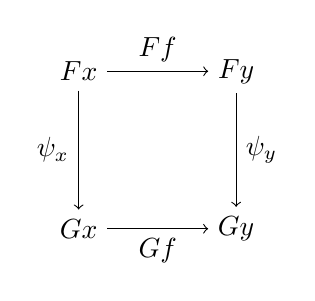
\begin{tikzpicture}
                    \node (FX) at (0, 0) {$Fx$};
                    \node (FY) at(2, 0) {$Fy$};
                    \node (GX) at (0, -2) {$Gx$};
                    \node (GY) at (2, -2) {$Gy$};
                    \draw[->] (FX) -- node[above]{$Ff$} (FY);
                    \draw[->] (GX) -- node[below]{$Gf$} (GY);
                    \draw[->] (FX) -- node[left]{$\psi_x$} (GX);
                    \draw[->] (FY) -- node[right]{$\psi_y$} (GY);
                \end{tikzpicture}
            \end{gather*}
        \end{enumerate}
    }
    \newdef{Functor category}{\index{functor!category}
        Consider two categories $\symbfsf{C}$ and $\symbfsf{D}$, where $\symbfsf{C}$ is small. The functors $\func{F}{C}{D}$ form the objects of a category with the natural transformations as morphisms. This category is denoted by $\funccat{C}{D}$ or $\symbfsf{D}^{\symbfsf{C}}$ (the latter is a generalization of \cref{set:function_set}).
    }

    \newdef{Dinatural transformation}{
        Consider two profunctors $\profunc{F,G}{C}{C}$ or, more generally, two functors $F,G:\symbfsf{C}^{\text{op}}\times\symbfsf{C}\rightarrow\symbfsf{D}$. A dinatural transformation is a family of morphisms \[\eta_x:F(x,x)\rightarrow G(x,x)\] that make Diagram~\ref{fig:dinatural} commute for every morphism $f:y\rightarrow x$.
    }

    \begin{figure}[ht!]
        \centering
        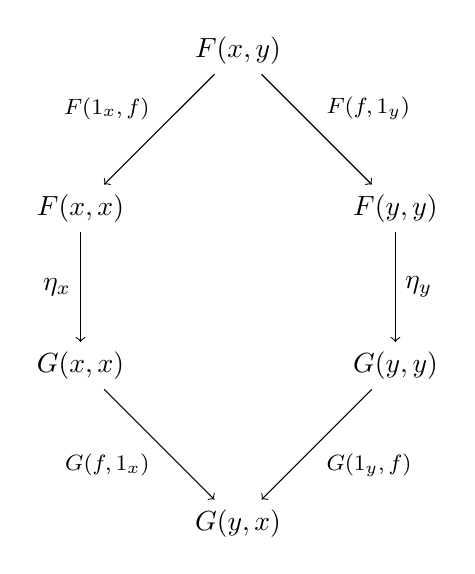
\begin{tikzpicture}
            \node (ab) at (0, 6) {$F(x,y)$};
            \node (F1) at (-2, 4) {$F(x,x)$};
            \node (F2) at (2, 4) {$F(y,y)$};
            \node (G1) at (-2, 2) {$G(x,x)$};
            \node (G2) at (2, 2) {$G(y,y)$};
            \node (ba) at (0, 0) {$G(y,x)$};

            \draw[->] (ab) edge node[above left]{\footnotesize$F(\mathbbm{1}_x,f)$} (F1) (F1) edge node[left]{$\eta_x$} (G1) (G1) edge node[below left]{\footnotesize$G(f,\mathbbm{1}_x)$} (ba);
            \draw[->] (ab) edge node[above right]{\footnotesize$F(f,\mathbbm{1}_y)$} (F2) (F2) edge node[right]{$\eta_y$} (G2) (G2) edge node[below right]{\footnotesize$G(\mathbbm{1}_y,f)$} (ba);
        \end{tikzpicture}
        \caption{Dinatural transformation.}
        \label{fig:dinatural}
    \end{figure}

    \newdef{Representable functor}{\index{representable}\index{representation}
        Let $\symbfsf{C}$ be a locally small category. A functor $\func{F}{C}{Set}$ is said to be representable if there exists an object $x\in\ob{C}$ such that $F$ is naturally isomorphic to $h^x$. The pair $(x,\psi:F\Rightarrow h^x)$ is called a \textbf{representation} of $F$.
    }

    \begin{theorem}[Yoneda lemma]\index{Yoneda!lemma}
        Let $\symbfsf{C}$ be a locally small category and let $\func{F}{C}{Set}$ be a functor. For every object $x\in\ob{C}$, there exists a natural isomorphism\footnote{Here, the fact that $\mathrm{Nat}(h^-,-)$ can be seen as a functor $\symbfsf{Set}^{\symbfsf{C}}\times\symbfsf{C}\rightarrow\symbfsf{Set}$ is used.}
        \begin{gather}
            \eta_x:\mathrm{Nat}(h^x,F)\rightarrow Fx:\psi\mapsto\psi_x(\mathbbm{1}_x)\,.
        \end{gather}
    \end{theorem}

    \begin{result}[Yoneda embedding]\index{Yoneda!embedding}
        When $F$ is another hom-functor $h^y$, the following result is obtained:
        \begin{gather}
            \mathrm{Nat}(h^x,h^y)\cong\symbfsf{C}(y,x)\,.
        \end{gather}
        Note that $y$ appears in the first argument on the right-hand side.

        Let $\symbfsf{C}(f,-)$ denote the natural transformation corresponding to the morphism $f\in\symbfsf{C}(y,x)$. The functor $h^-$, mapping an object $x\in\ob{C}$ to its hom-functor $\symbfsf{C}(x,-)$ and a morphism $f\in\symbfsf{C}(y,x)$ to the natural transformation $\symbfsf{C}(f,-)$, can also be interpreted as a covariant functor $G:\symbfsf{C}^{\text{op}}\rightarrow\symbfsf{Set}^{\symbfsf{C}}$. This way, the Yoneda lemma can be seen to give rise to an embedding $h^-$ of $\symbfsf{C}^{\text{op}}$ in the functor category $\symbfsf{Set}^{\symbfsf{C}}$.

        As usual, all of this can be done for contravariant functors. This gives an embedding
        \begin{gather}
            \mathcal{Y}:=h_-:\symbfsf{C}\hookrightarrow\symbfsf{Psh(C)}\,,
        \end{gather}
        called the Yoneda embedding.
    \end{result}

    \newdef{Local object}{\index{local!object}\label{cat:local_object}
        Consider a collection of morphisms $S\subseteq\mathrm{hom}(\symbfsf{C})$. An object $c\in\ob{C}$ is said to be $S$-local if the Yoneda embedding $\mathcal{Y}c$ maps morphisms in $S$ to isomorphisms in $\symbfsf{Set}$. A morphism $f\in\mathrm{hom}(\symbfsf{C})$ is said to be $S$-local if its image under the Yoneda embedding of every $S$-local object is an isomorphism in $\symbfsf{Set}$.
    }

\subsection{Equivalences}

    \newdef{Equivalence of categories}{\index{equivalence!of categories}
        Two categories $\symbfsf{C},\symbfsf{D}$ are said to be equivalent if there exist functors $\func{F}{C}{D}$ and $\func{G}{D}{C}$ such that $F\circ G$ and $G\circ F$ are naturally isomorphic to the identity functors.

        A weaker notion is that of a \textbf{weak equivalence}. Two categories $\symbfsf{C},\symbfsf{D}$ are said to be weakly equivalent if there exist functors $\func{F}{C}{D}$ and $\func{G}{D}{C}$ that are fully faithful and essentially surjective. Assuming the axiom of choice, every weak equivalence is also a (strong) equivalence (in fact this statement is equivalent to the axiom of choice).
    }

    \newdef{Skeletal category}{\index{category!skeletal}
        A category in which every isomorphism is necessarily an identity morphism. The \textbf{skeleton} of a category is an equivalent skeletal category (often taken to be a subcategory by choosing a representative from every isomorphism class).

        If one does not assume the axiom of choice, the skeleton is merely a weakly equivalent skeletal category.
    }

    \newdef{Decategorification}{\index{decategorification}\label{cat:decategorification}
        Let $\symbfsf{C}$ be an (essentially) small category. The set of isomorphism classes of $\symbfsf{C}$ is called the decategorification of $\symbfsf{C}$. This amounts to a functor $\func{\mathrm{Decat}}{Cat}{Set}$.
    }

\subsection{Stuff, structure and property}\index{forgetful}

    To classify properties of objects and the \textit{forgetfulness} of functors, it is interesting to make a distinction between stuff, structure and property. Consider for example a group. This is a set (\textit{stuff}) equipped with a number of operations (\textit{structure}) that obey some relations (\textit{properties}).

    Using these notions one can classify forgetful functors in the following way:
    \begin{itemize}
        \item A functor forgets nothing if it is an equivalence of categories.
        \item A functor forgets at most properties if it is fully faithful.
        \item A functor forgets at most structure if it is faithful.
        \item A functor forgets at most stuff if it is just a functor.
    \end{itemize}

    \todo{COMPLETE (see e.g. nLab or the paper ``Why surplus structure is not superfluous'' by Nicholas Teh et al.)}

\subsection{Adjunctions}\index{adjunction}\label{section:adjunction}

    \newdef{Hom-set adjunction}{
        Let $\func{F}{C}{D}$ and $\func{G}{D}{C}$ be two functors. These functors form a (hom-set) adjunction $F\dashv G$ if the following isomorphism is natural in both $x$ and $y$:
        \begin{gather}
            \Phi_{x,y}:\symbfsf{D}(Fx,y)\cong\symbfsf{C}(x,Gy)\,.
        \end{gather}
        The functor $F$ (resp.~$G$) is called the left (resp.~right) adjoint and the image of a morphism under either of the natural isomorphisms is called the adjunct of the other morphism.\footnote{The terms `adjunct' and `adjoint' are sometimes used interchangeably (cf.~French versus Latin).}.
    }
    \begin{notation}
        An adjunction $F\dashv G$ between categories $\symbfsf{C,D}$ is often denoted by \[\symbfsf{D}\adj{F}{G}\symbfsf{C}\,.\]
    \end{notation}

    \newdef{Unit-counit adjunction}{\index{triangle!identities}\index{unit}\index{zig-zag|see{triangle identity}}\label{cat:unit_counit_adjunction}
        Let $\func{F}{C}{D}$ and $\func{G}{D}{C}$ be two functors. These functors form a unit-counit adjunction if there exist natural transformations
        \begin{align}
            \varepsilon:F\circ G\Rightarrow\mathbbm{1}_{\symbfsf{D}}\\
            \eta:\mathbbm{1}_{\symbfsf{C}}\Rightarrow G\circ F
        \end{align}
        such that the following compositions are identity morphisms:
        \begin{align}
            F\overset{F\eta}{\longrightarrow}FGF&\overset{\varepsilon F}{\longrightarrow}F\,,\\
            G\overset{\eta G}{\longrightarrow}GFG&\overset{G\varepsilon}{\longrightarrow}G\,.
        \end{align}
        These identities are sometimes called the \textbf{triangle} or \textbf{zig-zag identities} (the latter results from the shape of the associated \textit{string diagram}). The transformations $\eta$ and $\varepsilon$ are called the \textbf{unit} and \textbf{counit}, respectively.
    }

    \begin{property}[Equivalence]
        Every hom-set adjunctions induces a unit-counit adjunction where the counit $\varepsilon_y$ is obtained as the adjunct $\Phi^{-1}_{Gy,y}(\mathbbm{1}_{Gy})$ of the identity morphism on $Gy\in\ob{C}$ and the unit $\eta_x$ is given by the adjunct $\Phi_{c,Fc}(\mathbbm{1}_{Fx})$ of the identity morphism at $Fx\in\ob{D}$.

        Conversely, every unit-counit adjunction induces a hom-set adjunction. The (right) adjunct of a morphism $f:Fx\rightarrow y$ is given by the composition
        \begin{gather}
            \widetilde{f}:=Gf\circ\eta_x:x\rightarrow (G\circ F)x\rightarrow Gy
        \end{gather}
        and the (left) adjunct of a morphism $\widetilde{g}:x\rightarrow Gy$ is given by:
        \begin{gather}
            g:=\varepsilon_y\circ F\tilde{g}:Fx\rightarrow(F\circ G)y\rightarrow y\,.
        \end{gather}
    \end{property}

    \newdef{Reflective subcategory}{\index{reflective!category}\index{localization!essential}\label{cat:reflective_inclusion}
        A full subcategory is said to be reflective (resp.~coreflective) if the inclusion functor admits a left (resp.~right) adjoint.
    }

    \begin{property}[Adjoint equivalence]\index{equivalence!adjoint}
        Any equivalence of categories is part of an adjoint equivalence, i.e.~an adjunction for which the unit and counit morphisms are invertible.
    \end{property}
    \begin{property}\label{cat:adjoint_equivalence}
        Given an adjunction, one obtains an adjoint equivalence by restricting to the full subcategories on which the unit and counit become isomorphisms.
    \end{property}

    Adjunctions can also be defined through a third alternative. This links the definition to universal properties.
    \newdef{Universal morphism}{\index{universal!morphism}\label{cat:universal_morphism}
        Consider a functor $\func{F}{C}{D}$ and an object $d\in\ob{D}$. A universal morphism from $d$ to $F$ is a pair $(c,f:d\rightarrow Fc)$ such that all other morphisms $f':d\rightarrow Fc'$ factor uniquely through $f$ by the image of a morphism in $\symbfsf{C}$.
    }
    \newadef{Adjoint functor}{
        A functor $\func{F}{C}{D}$ is a left adjoint if for each object $c\in\ob{C}$ there exists a universal morphism from $F$ to $c$. A functor $\func{G}{C}{D}$ is a right adjoint if for each object $d\in\ob{D}$ there exists a universal morphism from $d$ to $G$.

        The functor to which these functors are adjoint can be recovered as that mapping objects to the object-part of their universal morphism.
    }

\section{General constructions}

    \newdef{Dagger category}{\index{category!dagger}\label{cat:dagger_category}
        A category equipped with a contravariant involutive endofunctor, this functor is often denoted by $\func{\dagger}{C}{C}$, similar to the adjoint operator for Hermitian matrices.
    }
    \begin{remark}\index{unitary}\index{self-adjoint}
        The concept of a dagger structure allows the usual definition of \textbf{unitary} and \textbf{self-adjoint} morphisms, i.e.~morphism satisfying
        \begin{gather}
            f^\dagger = f^{-1}\qquad\text{or}\qquad f^\dagger = f\,.
        \end{gather}
    \end{remark}

    \newdef{Comma category}{\index{category!comma}
        Let $\symbfsf{A},\symbfsf{B}$ and $\symbfsf{C}$ be three categories and let $\func{F}{A}{C}$ and $\func{G}{B}{C}$ be two functors. The comma category $F\downarrow G$ is defined as follows:
        \begin{itemize}
            \item\textbf{Objects}: The triples $(x,y,\gamma)$ where $x\in\ob{A},y\in\ob{B}$ and $\gamma:Fx\rightarrow Gy$.
            \item\textbf{Morphisms}: The morphisms $(x,y,\gamma)\rightarrow(k,l,\sigma)$ are pairs $(f,g)$ with $f:x\rightarrow k\in\mathrm{hom}(\symbfsf{A})$ and $g:y\rightarrow l\in\mathrm{hom}(\symbfsf{B})$ such that $\sigma\circ Ff = Gg\circ\gamma$.
        \end{itemize}
        Composition of morphisms is defined componentwise.
    }
    \newdef{Arrow category}{\index{category!arrow}\index{walking!arrow}\index{interval!category}\label{cat:arrow_category}
        The comma category of the pair of functors $(\mathbbm{1}_{\symbfsf{C}},\mathbbm{1}_{\symbfsf{C}})$. This is equivalently the functor category $[\symbfsf{2},\symbfsf{C}]$, where $\symbfsf{2}$ is the \textbf{interval category/walking arrow} $\{0\rightarrow1\}$.
    }
    \newdef{Functorial factorization}{\index{factorization!functorial}\label{cat:functorial_factorization}
        A \textit{section} (see \cref{cat:retract}) of the composition functor \[\func{\circ}{[3,C]}{[2,C]}\,,\] where $\symbfsf{3}$ is the poset $\{0\rightarrow1\rightarrow2\}$.
    }

    If $F$ is the identity functor and $\func{G}{1}{C}$ picks out a single object, the notion of a slice category is obtained (by interchanging these choices, one can also define \textbf{coslice categories}).
    \newdef{Slice category}{\index{category!slice}\index{over!category}\label{cat:slice}
        Let $\symbfsf{C}$ be a category and consider an object $x\in\ob{C}$. The slice category (or \textbf{overcategory}) $\symbfsf{C}_{/x}$ of $\symbfsf{C}$ over $x$ is defined as follows:
        \begin{itemize}
            \item\textbf{Objects}: The morphisms in $\symbfsf{C}$ with codomain $x$, and
            \item\textbf{Morphisms}: The morphisms $f\rightarrow g$ are morphisms $h$ in $\symbfsf{C}$ such that $g\circ h = f$.
        \end{itemize}
        By dualizing one obtains the \textbf{undercategory} of $x$.
    }

\subsection{\difficult{Fibred categories}}\label{section:fibred_categories}

    \newdef{Fibre category}{\index{fibre!category}\label{cat:fibre_category}
        Let $\func{\Pi}{C}{D}$ be a functor. The fibre category (of $\Pi$) over $y\in\ob{D}$ is the subcategory of $\symbfsf{C}$ consisting of all objects $x\in\ob{C}$ such that $\Pi x=y$ and all morphisms $f\in\mathrm{hom}(\symbfsf{C})$ such that $\Pi f=\mathbbm{1}_y$. It will be denoted by $\symbfsf{C}_y$.

        Morphisms in $\symbfsf{C}$ that are mapped to a morphism $g$ in $\symbfsf{D}$ are called \textbf{$g$-morphisms} and, in particular (using the identification of objects and their identity morphisms), morphisms in $\symbfsf{C}_y$ are called \textbf{$y$-morphisms}. Similarly, \textbf{$\symbfsf{D}$-categories} are defined as the categories equipped with a (covariant) functor to $\symbfsf{D}$. (It is not hard to see that these form a \textit{2-category} under composition of functors that respects the $\symbfsf{D}$-category structure.)
    }

    \newdef{Cartesian morphism}{\index{Cartesian!morphism}
        Consider a $\symbfsf{D}$-category $\func{\Pi}{C}{D}$. A morphism $f$ in $\symbfsf{C}$ is called $\Pi$-Cartesian if every $\Pi f$-morphism factors uniquely through a $y$-morphism, where $y$ is the domain of $\Pi f$.

        There also exists a stronger notion. A \textbf{strongly Cartesian morphism} is a morphism $f\in\mathrm{hom}(\symbfsf{C})$ such that for every morphism $\varphi\in\mathrm{hom}(\symbfsf{C})$ with the same target and every factorization of $\Pi\varphi$ through $\Pi f$, there exists a unique factorization of $\varphi$ through $f$ that maps to the given factorization of $\Pi\varphi$.

        The following diagram, where the triangles commute, should clarify the above (technical) definitions:
        \begin{gather*}
            \begin{tikzpicture}
                \node (X3) at (0,2) {$\forall x'$};
                \node (X1) at (0,0) {$x_1$};
                \node (X2) at (2,0) {$x_2$};
                \node (arrow) at (4,1) {$\overset{\Pi}{\mapsto}$};
                \node (pX3) at (6,2) {$\Pi x'$};
                \node (pX1) at (6,0) {$\Pi x_1$};
                \node (pX2) at (8,0) {$\Pi x_2$};
                \draw[->] (X1) -- node[below]{$f$} (X2);
                \draw[->, dashed] (X3) -- node[left]{$\exists!g$} (X1);
                \draw[->] (X3) -- node[above right]{$\forall\varphi$} (X2);
                \draw[->] (pX1) -- node[below]{$\Pi f$} (pX2);
                \draw[->] (pX3) -- node[left]{$\forall\nu$} (pX1);
                \draw[->] (pX3) -- node[above right]{$\Pi\varphi$} (pX2);
            \end{tikzpicture}
        \end{gather*}
        The diagram for (weak) Cartesian morphisms is obtained by identifying the objects $\Pi x'$ and $\Pi x_1$, i.e.~by restricting to the case $\nu=\mathbbm{1}_{\Pi x_1}$.

        The Cartesian morphisms are said to be \textbf{inverse images} of their projections under $\Pi$ and the object $x_1$ is called an \textbf{inverse image} of $x_2$ by $\Pi f$. The Cartesian morphisms of a fibre category are exactly the isomorphisms of that category.
    }

    \newdef{Fibred category}{\index{fibred!category}\index{Grothendieck!fibration|see{fibred category}}
        A $\symbfsf{D}$-category $\func{\Pi}{C}{D}$ is called a fibred category or \textbf{Grothendieck fibration} if the following conditions are satisfied:
        \begin{enumerate}
            \item For each morphism in $\symbfsf{D}$, whose codomain lies in the range of $\Pi$, and each lift of this codomain to $\symbfsf{C}$, there exists at least one inverse image with the given codomain (in the weak sense).
            \item The composition of two Cartesian morphisms is again Cartesian (in the weak sense).
        \end{enumerate}
        If one instead works with strongly Cartesian morphisms, the second condition follows from the first one. However, it should be noted that, in a fibred category, a morphism is weakly Cartesian if and only if it is strongly Cartesian.
    }
    \newdef{Cleavage}{\index{cleavage}\index{cloven|see{cleavage}}
        Given a $\symbfsf{D}$-category $\func{\Pi}{C}{D}$, a cleavage is the choice of a Cartesian $g$-morphism $f:x\rightarrow y$ for every $y\in\ob{C}$ and morphism $g:d\rightarrow \Pi y$. A $\symbfsf{D}$-category equipped with a cleavage is said to be \textbf{cloven}.

        The existence of cleavage is sufficient for a category to be fibred and, conversely (assuming the axiom of choice), every fibred category admits a cleavage.
    }

    The following example can be obtained as a Grothendieck fibration with discrete fibres.
    \begin{example}[Discrete fibration]
        A functor $\func{F}{C}{D}$ such that, for every object $x\in\ob{C}$ and every morphism $f:y\rightarrow Fx$ in $\symbfsf{D}$, there exists a unique morphism $g:z\rightarrow x$ in $\symbfsf{C}$ such that $Fg=f$.
    \end{example}
    \begin{example}[Groupoidal fibration]
        If every morphism is required to be Cartesian, the notion of a groupoid(al) fibration or a \textbf{category fibred in groupoids} is obtained. The reason for this name is that every fibre is a groupoid. An equivalent definition is that the associated \textit{pseudofunctor} (see the construction below) factors through the embedding $\symbfsf{Grpd}\hookrightarrow\symbfsf{Cat}$.
    \end{example}

    \begin{property}[\difficult{Grothendieck construction}]\index{Grothendieck!construction}
        Every fibred category $\func{\Pi}{C}{D}$ defines a \textit{pseudofunctor}\footnote{See \cref{cat:pseudofunctor}.} $\cfunc{F}{D}{Cat}$ that sends objects to fibre categories and arrows $f:c\rightarrow c'$ to the pullback functor $f^*:\symbfsf{C}_{c'}\rightarrow\symbfsf{C}_c$ constructed from a Cartesian lift of $f$. This pullback functor acts as follows:
        \begin{itemize}
            \item For every object $x\in\symbfsf{C}_{c'}$, $f^*x$ is the domain of the Cartesian lift of $f$ through $x$.
            \item For every morphism $(\alpha:x\rightarrow y)\in\symbfsf{C}_{c'}$ there exists a diagram of the form
                \begin{gather*}
                    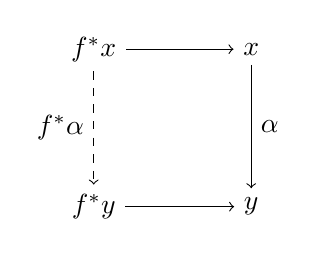
\begin{tikzpicture}
                        \node (fx) at (0, 0) {$f^*x$};
                        \node (x) at (2, 0) {$x$};
                        \node (y) at (2, -2) {$y$};
                        \node (fy) at (0, -2) {$f^*y$};
                        \draw[->] (fx) -- (x);
                        \draw[->] (fy) -- (y);
                        \draw[->] (x) -- node[right]{$\alpha$} (y);
                        \draw[dashed, ->] (fx) -- node[left]{$f^*\alpha$} (fy);
                    \end{tikzpicture}
                \end{gather*}
                Because the horizontal morphism are both projected to $f$ and $\alpha$ is projected to the identity, there exists a unique factorization of the diagram through a morphism $f^*\alpha:f^*x\rightarrow f^*y$.
        \end{itemize}

        Conversely, every \textit{pseudofunctor} gives rise to a fibred category through the Grothendieck construction $\int:\cfunccat{C}{Cat}\rightarrow\symbfsf{Cat}/\symbfsf{C}$ as follows. (These two constructions constitute a 2-equivalence of 2-categories.). Consider a \textit{pseudofunctor} $\cfunc{F}{C}{Cat}$. The `bundle' $\int\!F$ consists of the following data:
        \begin{itemize}
            \item The objects are pairs $(x,y)$ with $x\in\ob{C}$ and $y\in\mathrm{ob}(Fx)$.
            \item The morphisms $(x,y)\rightarrow(x',y')$ are pairs $\bigl(f:x\rightarrow x',\alpha:y\rightarrow Ff(y')\bigr)$.
        \end{itemize}
        Given a cleavage, the morphisms of the Grothendieck construction are exactly the factorizations of $f$-morphisms through the canonical lifting of $f$ in the cleavage.
    \end{property}
    \begin{property}[Functors]\index{split!cleavage}
        A \textit{pseudofunctor} is a functor if and only if the cleavage of the associated fibred category is \textbf{split(ting)}, i.e.~it contains all identities and is closed under composition.
    \end{property}

    \newdef{Category of elements}{\index{category!of elements}\label{cat:category_of_elements}
        Consider a presheaf $\cfunc{F}{C}{Set}$. Its category of elements $\mathrm{El}(F)$ or $\int_{\symbfsf{C}}F$ is defined as the comma category $(\mathcal{Y}\downarrow\ !_F)$, where $!_F:\ast\rightarrow\cfunccat{C}{Set}$ sends the unique object to $F$ itself. Equivalently, it is the category with objects the pairs $(c,x)\in\ob{C}\times Fc$ and morphisms $f\in\symbfsf{C}(c,c')$ such that $c = Ff(c')$, i.e.~it is the Grothendieck construction applied to $F$.

        This category comes equipped with a canonical forgetful functor
        \begin{gather}
            \symbfsf{C}_F:\mathrm{El}(F)\rightarrow\symbfsf{C}:(c,x)\mapsto c\,.
        \end{gather}
    }
    \remark{The category of elements is often defined for covariant functors. To obtain that definition, one should take the opposite of the category of elements (and also take the opposite of the forgetful functor).}

\subsection{Monads}

    \newdef{Monad}{\index{monad}\label{cat:monad}
        A monad is a triple $(T,\mu,\eta)$ where $\func{T}{C}{C}$ is an endofunctor and $\mu:T^2\rightarrow T, \eta:\mathbbm{1}_{\symbfsf{C}}\rightarrow T$ are natural transformations satisfying the following (coherence) conditions:
        \begin{enumerate}
            \item As natural transformations from $T^3$ to $T$:
            \begin{gather}
                \mu\circ T\mu = \mu\circ\mu_T\,.
            \end{gather}
            \item As natural transformations from $T$ to itself:
            \begin{gather}
                \mu\circ T\eta = \mu\circ\eta_T = \mathbbm{1}\,.
            \end{gather}
        \end{enumerate}
        These conditions say that a monad is a monoid (\cref{algebra:monoid}) in the category $\symbfsf{End}_{\symbfsf{C}}$ of endofunctors on $\symbfsf{C}$. Accordingly, $\eta$ and $\mu$ are often called the \textbf{unit} and \textbf{multiplication} maps.
    }

    \begin{example}[Adjunction]\label{cat:monad_from_adjunction}
        Every adjunction $F\dashv G$, with unit $\varepsilon$ and counit $\eta$, induces a monad of the form $(GF,G\varepsilon F,\eta)$.
    \end{example}

    \newdef{Algebra over a monad\footnotemark}{\index{algebra!over a monad}\index{module}\index{carrier}\label{cat:algebra_monad}
        \footnotetext{A more suitable name would be ``module over a monad'', since these are modules over a monoid if monads are regarded as monoids in $\symbfsf{End}_{\symbfsf{C}}$.}
        Consider a monad $(T,\mu,\eta)$ on a category $\symbfsf{C}$. An algebra over $T$ or $T$-algebra is a couple $(x,\kappa)$, where $x\in\ob{C}$ and $\kappa:Tx\rightarrow x$, such that the following conditions are satisfied:
        \begin{enumerate}
            \item $\kappa\circ T\kappa = \kappa\circ\mu_x$, and
            \item $\kappa\circ\eta_x = \mathbbm{1}_x$.
        \end{enumerate}
        Morphisms $(x,\kappa_x)\rightarrow(y,\kappa_y)$ of $T$-algebras are morphisms $f:x\rightarrow y$ in $\symbfsf{C}$ such that $f\circ\kappa_x = \kappa_y\circ Tf$. An algebra of the form $(Tx,\mu_x)$ is said to be \textbf{free}. The object $x$ is called the \textbf{carrier} of the algebra
    }
    \newdef{Eilenberg--Moore category}{\index{Eilenberg--Moore category}\label{cat:eilenberg_moore}
        Given a monad $T$ over a category $\symbfsf{C}$, the Eilenberg--Moore category $\symbfsf{C}^T$ is defined as the category of $T$-algebras.
    }
    \newdef{Kleisli category}{\index{Kleisli category}\label{cat:kleisli_category}
        Consider a monad $T$ on a category $\symbfsf{C}$. The Kleisli category $\symbfsf{C}_T$ is defined as the full subcategory of $\symbfsf{C}^T$ on the free $T$-algebras. This is equivalently the category with objects $\mathrm{ob}(\symbfsf{C}_T):=\ob{C}$ and morphisms $\symbfsf{C}_T(x,y):=\symbfsf{C}(x,Ty)$.

        Morphisms in the Kleisly category are composed in the `obvious way':
        \begin{gather}
            f\circ_{\symbfsf{C}_T} g := \mu_Z\circ Tf\circ g
        \end{gather}
        for all $f\in\symbfsf{C}_T(Y,TZ)$ and $g\in\symbfsf{C}_T(X,TY)$.
    }

    \newdef{Monadic adjunction}{\index{adjunction!monadic}
        Consider an adjunction $L\dashv R$ between categories $\symbfsf{C}$ and $\symbfsf{D}$ with the induced monad $T$. The natural morphism $R\varepsilon:T\circ R\Rightarrow R$ endows $R$ with a $T$-algebra structure and, hence, induces a functor $\symbfsf{C}\rightarrow\symbfsf{D}^T$ between $\symbfsf{C}$ and the Eilenberg-Moore category of $T$. $L\dashv R$ is said to be monadic if this functor is an equivalence.
    }
    \newdef{Monadic functor}{\index{functor!monadic}
        A functor is said to be monadic if it admits a left adjoint such that the adjunction is monadic.
    }

    The converse of \ref{cat:monad_from_adjunction} is also true:
    \begin{property}
        Every monad $\func{T}{C}{C}$ can be obtained from an adjunction. The canonical choice is the adjunction
        \begin{gather}
            \symbfsf{C}\adj{F_T}{U_T}\symbfsf{C}^T\,,
        \end{gather}
        where $F_T$ is the forgetful functor and $U_T$ sends an object to the free $T$-algebra on it.
    \end{property}

    The following theorem characterizes monadic functors (for more information on some of the concepts, see \cref{section:morphisms} further below).
    \begin{theorem}[Beck's monadicity theorem]\index{Beck's monadicity theorem}
        Consider a functor $\func{F}{C}{D}$. This functor is monadic if and only if the following conditions are satisfied:
        \begin{itemize}
            \item $F$ admits a left adjoint.
            \item $F$ reflects isomorphisms.
            \item $\symbfsf{C}$ has all coequalizers of $F$-split parallel pairs\footnote{These are parallel pairs $f,g$ such that the images $Ff,Fg$ under $F$ admit a split coequalizer.} and $F$ preserves these coequalizers.
        \end{itemize}
    \end{theorem}
    \begin{remark}[Crude monadicity theorem]
        A sufficient condition for monadicity is obtained by replacing the third condition above by the following weaker statement: ``$\symbfsf{C}$ has all coequalizers of reflexive pairs and $F$ preserves these coequalizers.''
    \end{remark}

    \newdef{Closure operator}{\index{closure!operator}\index{modal!operator|seealso{closure operator}}\index{modal!type}\label{cat:closure_operator}
        Consider a monad $(\func{T}{C}{C},\eta,\mu)$. This monad is called a closure operator or \textbf{modal operator} if the multiplication map is a natural isomorphism, i.e.~if the monad is idempotent. Equivalently, it is idempotent if and only if $\eta\circ T$ is a natural isomorphism.

        Given a closure operator $\func{T}{C}{C}$, the object $Tx$ is called the closure of $x\in\ob{C}$ and the associated morphism $\eta_x$ is called the \textbf{closing map}. An object $x\in\ob{C}$ itself is said to be $T$\textbf{-closed} exactly if its closing map is an isomorphism.

        An object $x\in\ob{C}$ is called a \textbf{modal type} if the unit $\eta_x:x\rightarrow Tx$ is an isomorphism.
    }
    \begin{property}
        Every (co)reflective subcategory inclusion (\cref{cat:reflective_inclusion}) induces a closure operator. Conversely, every closure operator is induced by a (co)reflective subcategory.
    \end{property}

    \begin{remark}[\difficult{Bicategories}]
        A monad can be defined in any bicategory as a 1-morphism $t:x\rightarrow x$ together with two 2-morphisms that satisfy conditions similar to the ones above. The above definition is then just a specific case of this more general definition in $\symbfsf{Cat}$.

        In the general setting one can then also define a \textbf{module} over a monad. First of all, one can regard any object $x\in\ob{C}$ as a functor from the terminal category $\symbfsf{1}$. By replacing $\symbfsf{1}$ by any other category in the ordinary definition one obtains a general algebra (or module). It is this definition that readily generalizes to bicategories, i.e.~a module is a 1-morphism $a:x\rightarrow y$ together with a 2-morphism that satisfies the same conditions as an algebra over a monad in $\symbfsf{Cat}$.
    \end{remark}

\section{Morphisms and diagrams}\label{section:morphisms}
\subsection{Morphisms}

    \newdef{Section}{\index{section}\index{retract}\label{cat:retract}
        A section of a morphism $f:x\rightarrow y$ is a right inverse, i.e.~a morphism $g:y\rightarrow x$ such that $f\circ g=\mathbbm{1}_y$. $f$ itself is called a \textbf{retraction} of $g$ and $y$ is called a \textbf{retract} of $x$.
    }

    \newdef{Monomorphism}{\index{monomorphism}
        Let $\symbfsf{C}$ be a category. A morphism $\mu\in\symbfsf{C}(x,y)$ is called a monomorphism, \textbf{mono} or \textbf{monic morphism} if for every object $z\in\ob{C}$ and every two morphisms $\alpha_1,\alpha_2\in\symbfsf{C}(z,x)$ such that $\mu\circ\alpha_1 = \mu\circ\alpha_2$, one can conclude that $\alpha_1=\alpha_2$.
    }
    \newdef{Epimorphism}{\index{epimorphism}
        Let $\symbfsf{C}$ be a category. A morphism $\varepsilon\in\symbfsf{C}(x,y)$ is called an epimorphism, \textbf{epi} or \textbf{epic morphism} if for every object $z\in\ob{C}$ and every two morphisms $\alpha_1,\alpha_2\in\symbfsf{C}(y,z)$ such that $\alpha_1\circ\varepsilon = \alpha_2\circ\varepsilon$, one can conclude that $\alpha_1=\alpha_2$.

        A family of morphisms $\{f_i:x_i\rightarrow y\}_{i\in I}$ is called \textbf{jointly epimorphic} if
        \begin{gather}
            \alpha_1\circ f_i = \alpha_2\circ f_i
        \end{gather}
        for all $i\in I$ implies that $\alpha_1=\alpha_2$.
    }

    \newdef{Split monomorphism}{\index{split!morphism}
        A morphism $f:x\rightarrow y$ that is a section of some other morphism $g:y\rightarrow x$. It can be shown that every split mono is in fact a mono and even an \textbf{absolute mono}, i.e.~it is preserved by all functors.

        The morphism $g$ can be seen to satisfy the dual condition and, hence, is called a \textbf{split epimorphism}. It can be shown to be an absolute epi.
    }

    \newdef{Balanced category}{\index{category!balanced}\label{cat:balanced}
        A category in which every monic epi is an isomorphism.
    }

    \newdef{Reflexive pair}{
        Two parallel morphisms $f,g:x\rightarrow y$ are said to form a reflexive pair if they have a common section, i.e.~if there exists a morphism $\sigma:y\rightarrow x$ such that $f\circ\sigma=g\circ\sigma=\mathbbm{1}_y$.
    }

    \newdef{Subobject}{\index{subobject}
        Let $\symbfsf{C}$ be a category and let $x\in\ob{C}$ be any object. A subobject $y$ of $x$ is a mono $y\hookrightarrow x$.

        In fact, one should work up to isomorphisms and, accordingly, the formal definition goes as follows: a subobject $y$ of $x$ is an isomorphism class of monos $i:y\hookrightarrow x$ in the slice category $\symbfsf{C}_{/x}$.
    }
    \newdef{Well-powered category}{\index{well-!powered}
        A category $\symbfsf{C}$ such that for every object $x\in\ob{C}$ the class of subobjects $\mathrm{Sub}(x)$ is small.
    }

\subsection{Initial and terminal objects}

    \newdef{Initial object}{\index{initial}
        An object $\emptyset$ such that for every other object $x$ there exists a unique morphism $\iota_x:\emptyset\rightarrow x$. If one drops the uniqueness, the notion of a \textbf{weakly initial object} is obtained.
    }
    \newdef{Terminal object}{\index{terminal}
        An object $1$ such that for every other object $x$ there exists a unique morphism $\tau_x:x\rightarrow 1$.
    }
    \begin{property}[Uniqueness]
        If an initial (or terminal) object exists, it is unique (up to isomorphisms).
    \end{property}

    \newdef{Zero object}{\index{zero!object}\label{cat:zero_object}
        An object that is both initial and terminal. The zero object is often denoted by $0$.
    }
    \begin{property}[Zero morphism]
        From the definition of the zero object it follows that for any two objects $x,y$ there exists a unique morphism $0_{xy}:x\rightarrow0\rightarrow y$.
    \end{property}
    \newdef{Pointed category}{\index{pointed!category}\label{cat:pointed_category}
        A category containing a zero object.
    }

    \newdef{Global element}{\index{global!element}\label{cat:global_element}
        Let $\symbfsf{C}$ be a category with a terminal object $1$. A global element of an object $x\in\ob{C}$ is a morphism $1\rightarrow x$.
    }
    \begin{property}
        Every global element is monic.
    \end{property}

    \newdef{Pointed object}{\index{pointed!object}\label{cat:pointed_object}
        An object $x$ equipped with a global element $1\rightarrow x$. This morphism is sometimes called the \textbf{basepoint}.
    }

    \begin{remark}\label{cat:global_elements_remark}
        In the category $\symbfsf{Set}$, the elements of a set $S$ are in one-to-one correspondence with the global elements of $S$. Furthermore, there is the the important property (\textit{axiom of functional extensionality}) that two functions $f,g:S\rightarrow S'$ coincide if their values at every element $s\in S$ coincide or, equivalently, if their precompositions with global elements coincide.

        However, this way of checking equality can fail in other categories. Consider for example $\symbfsf{Grp}$, the category of groups, with its zero object $0=\{e\}$. The only morphism from this group to any other group $G$ is the one mapping $e$ to the unit in $G$. It is obvious that precomposition with this morphism says nothing about the equality of other morphisms. To recover the extensionality property from $\symbfsf{Set}$, the notion of an `element' should be generalized:
    \end{remark}
    \newdef{Generalized element}{\index{shape}
        Let $\symbfsf{C}$ be a category and consider an object $x\in\ob{C}$. For any object $y\in\ob{C}$, a morphism $y\rightarrow x$ is called a generalized element of $x$. These morphisms are also called \textbf{$y$-elements} in $x$ or elements of \textbf{shape} $y$ in $x$.
    }

    \newdef{Generator}{\index{generator}\index{separator|see{generator}}\label{cat:generator}
        Let $\symbfsf{C}$ be a category. A collection of objects $\mathcal{O}\subset\ob{C}$ is called a collection of generators or \textbf{separators} for $\symbfsf{C}$ if the generalized elements of shape $\mathcal{O}$ are sufficient to distinguish between all morphisms in $\symbfsf{C}$:
        \begin{gather}
            \forall x,y\in\ob{C}:\forall f,g\in\symbfsf{C}(x,y):\bigl(f\neq g\implies\exists o\in\mathcal{O}:\exists h\in\symbfsf{C}(o,x): f\circ h\neq g\circ h\bigr)\,.
        \end{gather}
    }
    \newdef{Well-pointed category}{\index{well-!pointed}
        A category for which the terminal object is a generator.
    }

    \newdef{Free object}{\index{free}
        Consider a forgetful functor $\func{U}{C}{D}$ (whatever this may mean). An object $c\in\ob{C}$ is said to be free over an object $x\in\ob{D}$ if there exists a universal morphism $\eta_x:x\rightarrow Uc$. These are the initial objects of the comma categories $x/\symbfsf{U}$.
    }
    \begin{property}[Free functor]\index{free!functor}
        Note that if the forgetful functor admits a left adjoint $\func{F}{D}{C}$, every object in the image of $F$ is free according to the previous definition. Moreover, if $U$ admits a free object for every $x\in\ob{D}$, it has a left adjoint. For this reason, left adjoints to fortgetful functors are often called free functors.
    \end{property}

    \Cref{cat:algebra_monad} can be generalized to endofunctors as follows:
    \newdef{Algebra over an endofunctor}{\index{carrier}\label{cat:endofunctor_algebra}
        Consider an endofunctor $\func{F}{C}{C}$. An algebra over $F$ is a pair $(x,f:Fx\rightarrow x)$, where $x\in\ob{C}$ is often called the \textbf{carrier}.
    }
    \begin{property}\label{cat:algebraically_free_monad}
        The category of algebras over an endofunctor is equivalent to the Eilenberg--Moore category of the \textbf{(algebraically-)free monad} it generates (if it exists).
    \end{property}
    \begin{construct}
        This property could actually be interpreted as the definition of the free monad generated by an endofunctor. If it exists, it can be obtained as the monad induced by the free-forgetful adjunction induced by $F\symbfsf{Alg}\rightarrow\symbfsf{C}$.

        When the free functor exists, it can be constructed as follows. Consider an endofunctor $\func{F}{C}{C}$. The term introduction of an inductive type corresponds to a morphism $Fc\rightarrow c$, i.e.~to an algebra over $F$. Now, algebras over $F$ should correspond to the algebras over its free monad, the functor $F^*:=U\circ\mathcal{F}$, where $U:F\symbfsf{Alg}\rightarrow\symbfsf{C}$ is the forgetful functor and $\mathcal{F}:\symbfsf{C}\rightarrow F\symbfsf{Alg}$ the free functor. The latter sends every object $d\in\ob{C}$ to the initial object of the comma category $d/U$, i.e.~to an object $(c,\alpha: Fc\rightarrow c,\beta:d\rightarrow c)$. However, as long as $\symbfsf{C}$ admits coproducts, such a triple is equivalent to a pair $(c,\gamma:d+Fc\rightarrow c)$. Since the latter is an algebra over $\mathbbm{1}_{\symbfsf{C}}+F$, one finds that algebras over $F$ are equivalent to initial algebras over $\mathbbm{1}_{\symbfsf{C}}+F$.
    \end{construct}

    \begin{theorem}[Lambek]
        If $\func{F}{C}{C}$ has an initial algebra $f:Fx\rightarrow x$, then $f$ is an isomorphism.
    \end{theorem}

\subsection{Lifts}

    \newdef{Lifts and extensions}{\index{lift}\index{extension}
        A lift of a morphism $f:x\rightarrow y$ along an epi $e:z\rightarrow y$ is a morphism $g:x\rightarrow z$ satisfying $f=e\circ g$. Dualizing this definition gives the notion of extensions. (The epi/mono condition is often dropped in the literature.)
    }
    \newdef{Lifting property}{\index{orthogonal!lifting}\label{cat:lifting_property}
        A morphism $f:x\rightarrow y$ has the left lifting property with respect to a morphism $g:x'\rightarrow y'$ (or $g$ has the right lifting property with respect to $f$) if for every commutative diagram
        \begin{gather*}
            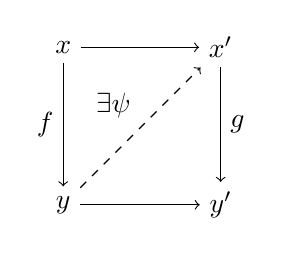
\begin{tikzpicture}
                \node (A) at (0, 0) {$x$};
                \node (B) at (0, -2) {$y$};
                \node (C) at (2, 0) {$x'$};
                \node (D) at (2, -2) {$y'$};
                \draw[->] (A) -- node[left]{$f$} (B);
                \draw[->] (A) -- (C);
                \draw[->, dashed] (B) -- node[above left]{$\exists\psi$} (C);
                \draw[->] (B) -- (D);
                \draw[->] (C) -- node[right]{$g$} (D);
            \end{tikzpicture}
        \end{gather*}
        there exists a morphism $\psi:y\rightarrow x'$ such that the triangles commute. If the morphism $\psi$ is unique, then $f$ and $g$ are said to be \textbf{orthogonal}.
    }
    \newdef{Injective / projective morphisms}{\index{injective!morphism}\index{projective!morphism}
        Consider a class of morphisms $I\subseteq\mathrm{hom}(\symbfsf{C})$. A morphism $f\in\mathrm{hom}(\symbfsf{C})$ is said to be $I$-injective (resp.~$I$-projective) if it has the right (resp.~left) lifting property with respect to all morphisms in $I$.

        Given a set of morphisms $I$, the sets of $I$-injective and $I$-projective morphisms are denoted by $\mathrm{rlp}(I)$ and $\mathrm{llp}(I)$, respectively.
    }
    \newdef{Injective and projective objects}{\index{injective!object}\index{projective!object}
        If $\symbfsf{C}$ has a terminal object $1$, an object $x$ is called $I$-injective if its terminal morphism is $I$-injective. If $\symbfsf{C}$ has an initial object, $I$-projective objects can be defined dually. (See \cref{fig:inj_proj}.)

        \begin{figure}[ht!]
            \centering
            \begin{subfigure}[b]{0.49\textwidth}
                \centering
                \begin{tikzpicture}
                    \node (X) at (0, 0) {$x$};
                    \node (Y) at (0, -2) {$y$};
                    \node (C) at (2, 0) {$i$};
                    \draw[->] (X) -- node[left]{$\forall f\in I$} (Y);
                    \draw[->] (X) -- node[above]{$g$} (C);
                    \draw[dashed, ->] (Y) -- node[below right]{$\exists\psi$} (C);
                \end{tikzpicture}
                \caption{Injective object $i$.}
                \label{fig:injective_object}
            \end{subfigure}
            \begin{subfigure}[b]{0.49\textwidth}
                \centering
                \begin{tikzpicture}
                    \node (X) at (2, 2) {$x$};
                    \node (Y) at (2, 0) {$y$};
                    \node (C) at (0, 0) {$p$};
                    \draw[->] (X) -- node[right]{$\forall f\in I$} (Y);
                    \draw[->] (C) -- node[below]{$g$} (Y);
                    \draw[dashed, ->] (C) -- node[above left]{$\exists\psi$} (X);
                \end{tikzpicture}
                \caption{Projective object $p$.}
                \label{fig:projective_object}
            \end{subfigure}
            \caption{Injective and projective objects.}
            \label{fig:inj_proj}
        \end{figure}
        If $I$ is the class of monomorphisms (resp.~epimorphisms), the terminology is simplified to \textbf{injective} (resp.~\textbf{projective}) objects. For projective objects, this is also equivalent to requiring that the (covariant) hom-functor preserves epimorphisms.

        A category $\symbfsf{C}$ is said to \textbf{have enough injectives} if, for every object, there exists a monomorphism into an injective object. The category is said to \textbf{have enough projectives} if, for every object, there exists an epimorphism from a projective object.
    }
    \newdef{Fibrations and cofibrations}{\index{fibration}
        Consider a category $\symbfsf{C}$ together with a class $I\subseteq\mathrm{hom}(\symbfsf{C})$ of morphisms. A morphism $f\in\mathrm{hom}(\symbfsf{C})$ is called an $I$-fibration (resp. $I$-cofibration) if it has the right (resp.~left) lifting property with respect to all $I$-projective (resp.~$I$-injective) morphisms.
    }

\subsection{Limits and colimits}\label{section:diagrams}

    \newdef{Diagram}{\index{diagram}
        A diagram in $\symbfsf{C}$ with index category $\symbfsf{I}$ is a (covariant) functor $\func{D}{I}{C}$.
    }

    \newdef{Cone}{\index{cone}
        Let $\func{D}{I}{C}$ be a diagram. A cone from $c\in\ob{C}$ to $D$ consists of a family of morphisms $\psi_i:c\rightarrow Di$ indexed by $\symbfsf{I}$ such that $\psi_j = Df\circ\psi_i$ for all morphisms $f:i\rightarrow j\in\mathrm{hom}(\symbfsf{I})$. (This is depicted in \cref{fig:cone_component}.)

        \begin{figure}[ht!]
            \centering
            \begin{subfigure}[b]{0.49\textwidth}
                \centering
                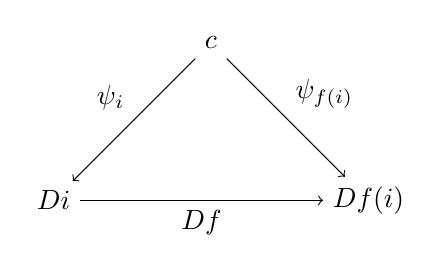
\begin{tikzpicture}
                    \node (1) at (0, 0) {$c$};
                    \node (2) at (-2, -2) {$Di$};
                    \node (3) at (2, -2) {$Df(i)$};
                    \draw[->] (1) -- node[above left]{$\psi_i$} (2);
                    \draw[->] (1) -- node[above right]{$\psi_{f(i)}$} (3);
                    \draw[->] (2) -- node[below]{$Df$} (3);
                \end{tikzpicture}
                \caption{Component of cone over $D$.}
                \label{fig:cone_component}
            \end{subfigure}
            \begin{subfigure}[b]{0.49\textwidth}
                \centering
                \begin{tikzpicture}
                    \node (1) at (0, -2) {$Di$};
                    \node (2) at (-2, 0) {$a$};
                    \node (3) at (2, 0) {$b$};
                    \draw[<-] (1) -- node[below left]{$\psi_i$} (2);
                    \draw[<-] (1) -- node[below right]{$\phi_i$} (3);
                    \draw[->] (2) -- node[above]{$f$} (3);
                \end{tikzpicture}
                \caption{Morphism of cones.}
                \label{fig:cone_morphism}
            \end{subfigure}
            \caption{Category of cones.}
            \label{fig:cone}
        \end{figure}
    }
    \begin{adefinition}\index{diagonal!functor}
        The above definition can be reformulated by defining an additional functor $\Delta_x:\symbfsf{I}\rightarrow\symbfsf{C}$ that maps every element $i\in\ob{I}$ to $x$ and every morphism $g\in\mathrm{hom}(\symbfsf{I})$ to $\mathbbm{1}_x$, i.e.~$\Delta:C\rightarrow[\symbfsf{I},\symbfsf{C}]$ is the \textbf{diagonal functor}. The morphisms $\psi_i$ can then be seen to be the components of a natural transformation $\psi:\Delta_x\Rightarrow D$. Hence, a cone $(x,\psi)$ is an element of $[\symbfsf{I},\symbfsf{C}](\Delta_x,D)$.
    \end{adefinition}
    \newdef{Morphism of cones}{\index{morphism!of cones}
        Let $\func{D}{I}{C}$ be a diagram and let $(x,\psi)$ and $(y,\phi)$ be two cones over $D$. A morphism between these cones is a morphism of the apexes $f:x\rightarrow y$ such that the diagrams of the form \ref{fig:cone_morphism} commute for all $i\in\ob{I}$. The cones over $D$ together with these morphisms form a category $\symbfsf{Cone}(D)$. In fact this can easily be seen to be the comma category $\Delta\downarrow D$.
    }

    \newdef{Limit}{\index{limit}\label{cat:limit}
        Consider a diagram $\func{D}{I}{C}$. The limit of this diagram, denoted by $\lim D$, is (if it exists) the terminal object of the category $\symbfsf{Cone}(D)$.
    }
    \begin{remark}\index{projective!limit}\index{inductive!limit}\label{cat:projective_remark}
        In the older literature, the name \textbf{projective limit} was sometimes used. The dual notion, a \textbf{colimit}, was often called an \textbf{inductive limit} in the older literature.
    \end{remark}

    This definition leads to the following universal property.
    \begin{uproperty}\label{cat:limit_uproperty}
        Let $\func{D}{I}{C}$ be a diagram. For every cone $(x,\psi)\in\symbfsf{Cone}(D)$, there exists a unique morphism $f:x\rightarrow\lim D$. This defines a bijection
        \begin{gather}
            \funccat{I}{C}(\Delta_x,D)\cong\symbfsf{C}(x,\lim D)\,.
        \end{gather}
        If all (small) limits exist, the limit functor $\func{\lim}{[I,C]}{C}$ can be defined. The universal property of limits then implies that it is right adjoint to the constant functor $\Delta$.

        For diagrams in $\symbfsf{Set}$, one can use the fully faithfulness of the Yoneda embedding to obtain the following expression:
        \begin{gather}
            \lim D\cong\funccat{I}{Set}(\Delta_\ast,D)\,.
        \end{gather}
    \end{uproperty}
    \begin{remark}
        In \cref{section:enriched_category_theory} on enriched category theory, a generalization of the above construction (the so-called \textit{weighted limits}) will be given that is better suited to the enriched setting and allows to express a wide variety of constructions as (weighted) limits.
    \end{remark}

    \begin{example}[Terminal object]
        The terminal object $1$ is the limit of the empty diagram.
    \end{example}

    \newdef{Finitely complete category}{\index{category!complete}
        A category is said to be finitely complete if it has all finite limits. If all (small) limits exist, the category is said to be \textbf{complete}. The dual notion for colimits is called \textbf{(finite) cocompleteness}.
    }
    \begin{example}[Presheaf categories]\label{cat:complete_presheaf_category}
        All presheaf categories are both complete and cocomplete.
    \end{example}

    \newdef{Continuous functor}{\index{continuity!functor}\label{cat:continuity}
        A functor that preserves all small limits.
    }
    A more restricted form is also common in the literature.
    \newdef{Exact functor}{\index{exact!functor}\label{cat:exact_functor}
        A functor that preserves all finite limits is said to be \textbf{left exact}. Analogously, a functor that preserves all finite colimits is said to be \textbf{right exact}.
    }

    \begin{example}[Hom-functors]
        In a locally small category every hom-functor is continuous (in fact these functors even preserve limits that are not necessarily small). This implies for example that
        \begin{gather}
            \symbfsf{C}(x,\lim D)\cong\lim\symbfsf{C}(x,D)\,.
        \end{gather}
    \end{example}

    In the case where $\symbfsf{C}$ is small, one can characterize the Yoneda embedding through a universal property:
    \begin{uproperty}[Free cocompletion]\index{co-!completion}\label{cat:free_cocompletion}
        The Yoneda embedding $\symbfsf{C}\hookrightarrow\widehat{\symbfsf{C}}$ turns the presheaf category $\widehat{\symbfsf{C}}$ into the \textbf{free cocompletion} of $\symbfsf{C}$, i.e.~there exists an equivalence of categories between the functor category of cocontinuous functors $[\widehat{\symbfsf{C}},\symbfsf{D}]_{\mathrm{cont}}$ and the ordinary functor category $[\symbfsf{C},\symbfsf{D}]$.
    \end{uproperty}

    \newdef{Tiny object}{\index{tiny}\label{cat:tiny}
        An object in a locally small category for which the covariant hom-functor preserves small colimits. This is sometimes called a \textbf{small-projective} object since it is, in particular, projective\footnote{Epimorphisms are characterized by a \textit{pushout} (see \cref{cat:pushout_epi} further below).}.
    }
    \newdef{Cauchy completion}{\index{Cauchy!completion}\index{Karoubi!envelope}
        Let $\symbfsf{C}$ be a small category. An important (small and full) subcategory of the free cocompletion of $\symbfsf{C}$ is given by the Cauchy completion, i.e.~the subcategory of $\widehat{\symbfsf{C}}$ on the tiny objects.\footnote{A generalization in the context of enriched categories is given by the \textit{Karoubi envelope}.} It can be shown that the free cocompletion of the Cauchy completion coincides with the one on $\symbfsf{C}$ (up to equivalence).

        A category is said to be \textbf{Cauchy-complete} if it is equivalent to its Cauchy completion. It can be shown that a category is Cauchy-complete if and only if it has all small absolute colimits.
    }

    \newdef{Filtered category}{\index{category!filtered}\label{cat:filtered}
        A category in which every finite diagram admits a cocone. For regular cardinals $\kappa$, this notion can be generalized. A category is said to be $\kappa$-filtered if every diagram with less than $\kappa$ arrows admits a cocone. (In this terminology, filtered categories are the same as $\omega$-filtered categories.)
    }

    \newdef{Directed limit}{\index{limit!directed}
        Consider a diagram $\func{D}{I}{C}$. The limit (resp.~colimit) of $D$ is said to be (co)directed (resp.~directed) if $\symbfsf{I}$ is a downward (resp.~upward) directed set \ref{set:directed_set}.
    }
    The following definition is a categorification of the previous one.
    \newdef{Filtered limit}{\index{limit!filtered}
        Consider a diagram $\func{D}{I}{C}$. The limit (resp.~colimit) of $D$ is said to be (co)filtered (resp.~filtered) if $\symbfsf{I}$ is a cofiltered (resp.~filtered) category.
    }
    \begin{property}\label{cat:directed_filtered}
        A category has all directed limits if and only if it has all filtered limits. (A dual statement holds for colimits.)
    \end{property}

    \newdef{Finitary functor}{\index{functor!finitary}\label{cat:finitary_functor}
        A functor that preserves all filtered colimits.
    }

    \newdef{Pro-object}{\index{pro-!object}\label{cat:pro_object}
        A functor $\func{F}{I}{C}$ from a cofiltered category. By composing these functors with the Yoneda embedding $\func{\mathcal{Y}}{C}{\cfunccat{C}{Set}}$, pro-objects can also be identified with cofiltered limits of representable presheaves. In conjunction with \cref{cat:projective_remark}, this clarifies the terminology.
    }
    \begin{uproperty}\index{pro-!category}\label{cat:pro_object_uproperty}
        The \textbf{procategory} $\symbfsf{Pro(C)}$ is the universal completion of $\symbfsf{C}$ under cofiltered limits. $\symbfsf{Pro(C)}$ satisfies (cf.~\cref{cat:free_cocompletion}):
        \begin{itemize}
            \item it admits all cofiltered limits, and
            \item if $\symbfsf{D}$ admits all cofiltered limits, there is an equivalence of functor categories
            \begin{gather}
                \funccat{C}{D}\cong\symbfsf{Fin}\bigl(\symbfsf{Pro(C)},\symbfsf{D}\bigr)\,,
            \end{gather}
            where the category on the right-hand side is the category of finitary functors.
        \end{itemize}
    \end{uproperty}
    \begin{remark}[Ind-objects]\index{ind-object}
        By dualizing the above definitions, i.e.~by replacing cofiltered limits by filtered colimits, the category of ind-objects $\symbfsf{Ind(C)}$ is obtained.
    \end{remark}

    \newdef{Compact object}{\index{compact}\index{presentable}\label{cat:compact}
        An object for which the covariant hom-functor preserves all filtered colimits. These objects are also said to be \textbf{finitely presentable}.\footnote{This name derives from the fact that modules are finitely presented if and only if their covariant hom-functor preserves direct limits (i.e.~directed colimits in the context of algebra).}
    }

    \newdef{Product}{\index{product}\index{co-!product}\label{cat:product}
        Let $\symbfsf{I}$ be a discrete category. The (co)limit over a diagram $\func{D}{I}{C}$ is called a (co)product in $\symbfsf{C}$.
    }

    \begin{example}[Equalizer]\index{equalizer}\index{fork}
        Consider a diagram of the form \[x\overset{f}{\underset{g}{\rightrightarrows}}y\,.\] The limit of this diagram is called the equalizer of $f$ and $g$. It consists of an object $e$ and a morphism $\varepsilon:e\rightarrow x$ such that the following \textbf{fork} diagram
        \begin{gather}
            e\overset{\varepsilon}{\rightarrow}x\overset{f}{\underset{g}{\rightrightarrows}}y
        \end{gather}
        is universal with respect to $(e,\varepsilon)$. By dualizing one obtains \textbf{cofork} diagrams $x\rightrightarrows y\rightarrow z$ and their universal versions, the \textbf{coequalizers}.
    \end{example}
    \begin{example}[Split coequalizer]\index{split!morphism}\label{cat:split_coequalizer}
        A cofork diagram \[x\overset{f}{\underset{g}{\rightrightarrows}}y\overset{\tau}{\rightarrow}z\] together with a section $\varphi$ of $f$ and a section $\sigma$ of $\tau$ such that $\sigma\circ\tau = g\circ\varphi$.
    \end{example}

    \newdef{Regular morphisms}{\index{regular!morphism}
        A mono (resp.~epi) is said to be regular if it arises as an equalizer (resp.~coequalizer) of two parallel morphisms.
    }

    Although not all categories are balanced (\cref{cat:balanced}), the following property does hold in any category.
    \begin{property}[Regular bimorphism]\index{bi-!morphism}\label{cat:regular_iso}
        Both monic regular epimorphisms and epic regular monomorphisms are isomorphisms.
    \end{property}

    \newadef{Finitely complete category}{\index{category!complete}\label{cat:finitely_complete_alternative}
        A category is said to be finitely complete if it has a terminal object and if all binary equalizers and products exist.
    }

    \newdef{Span}{\index{span}\label{cat:span}
        A span in a category $C$ is a diagram of the form~\ref{fig:cat_span}. By definition of a diagram, a span in $C$ is equivalent to a functor $\func{S}{\symbf{\Lambda}}{C}$, where $\symbfsf{\symbf{\Lambda}}$ is the category with three objects $\{-1,0,1\}$ and two morphisms $i:0\rightarrow -1$ and $j:0\rightarrow 1$. For this reason $\symbfsf{\symbf{\Lambda}}$ is sometimes called the walking or universal span.

        \begin{figure}[!ht]
            \centering
            \begin{subfigure}[b]{0.49\textwidth}
                \centering
                \begin{tikzpicture}
                    \node (X) at (-2, 0) {$x$};
                    \node (S) at (0, 2) {$s$};
                    \node (Y) at (2, 0) {$y$};
                    \draw[->] (S) -- node[above left]{$f$} (X);
                    \draw[->] (S) -- node[above right]{$g$} (Y);
                \end{tikzpicture}
                \caption{Span (category theory).}
                \label{fig:cat_span}
            \end{subfigure}
            \begin{subfigure}[b]{0.49\textwidth}
                \centering
                \begin{tikzpicture}
                    \node (X) at (-2, 2) {$x$};
                    \node (S) at (0, 0) {$c$};
                    \node (Y) at (2, 2) {$y$};
                    \draw[<-] (S) -- node[below left]{$f$} (X);
                    \draw[<-] (S) -- node[below right]{$g$} (Y);
                \end{tikzpicture}
                \caption{Cospan.}
                \label{fig:pullback}
            \end{subfigure}
            \caption{(Co)span diagrams.}
        \end{figure}
    }

    \newdef{Pullback}{\index{pullback}\index{Cartesian!square}\label{cat:pullback}
        The pullback of two morphisms $f:x\rightarrow z$ and $g:y\rightarrow z$ is defined as the limit of cospan~\ref{fig:pullback}. The full diagram characterizing the pullback, which has the form of a square, is sometimes called a \textbf{Cartesian square}.
    }
    \begin{notation}[Pullback]
        The pullback of two morphisms $f:x\rightarrow z$ and $g:y\rightarrow z$ is often denoted by $x\times_zy$. The associated pullback square is sometimes written as in \cref{fig:pullback_square}.

        \begin{figure}[ht!]
            \centering
            \begin{subfigure}[b]{0.49\textwidth}
                \centering
                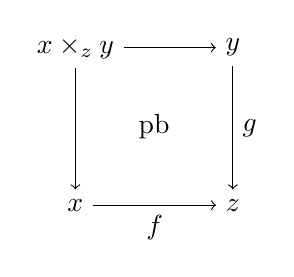
\begin{tikzpicture}
                    \node (X) at (0, -2) {$x$};
                    \node (Y) at (2, 0) {$y$};
                    \node (Z) at (2, -2) {$z$};
                    \node (pull) at (0, 0) {$x\times_zy$};
                    \node at (1, -1) {pb};
                    \draw[<-] (Z) -- node[below]{$f$} (X);
                    \draw[<-] (Z) -- node[right]{$g$} (Y);
                    \draw[->] (pull) -- (X);
                    \draw[->] (pull) -- (Y);
                \end{tikzpicture}
                \caption{Pullback square.}
                \label{fig:pullback_square}
            \end{subfigure}
            \begin{subfigure}[b]{0.49\textwidth}
                \centering
                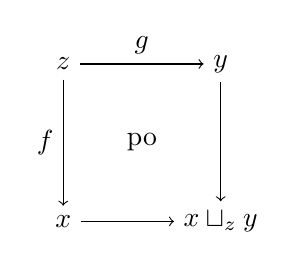
\begin{tikzpicture}
                    \node (X) at (0, -2) {$x$};
                    \node (Y) at (2, 0) {$y$};
                    \node (Z) at (0, 0) {$z$};
                    \node (push) at (2, -2) {$x\sqcup_zy$};
                    \node at (1, -1) {po};
                    \draw[->] (Z) -- node[left]{$f$} (X);
                    \draw[->] (Z) -- node[above]{$g$} (Y);
                    \draw[<-] (push) -- (X);
                    \draw[<-] (push) -- (Y);
                \end{tikzpicture}
                \caption{Pushout square.}
                \label{fig:pushout_square}
            \end{subfigure}
            \caption{Pullback and pushout diagrams.}
        \end{figure}
    \end{notation}

    \begin{example}[Product]\index{product}\index{fibre!product}
        If a terminal object $1$ exists, the pullback $x\times_1y$ is equal to the product $x\times y$.

        In fact, pullbacks are sometimes also called \textbf{fibred products}. The reason for this terminology is not only that products reduce to a particular case, but also that in the case of $\symbfsf{Set}$ the pullbacks have a fibrewise product structure:
        \begin{gather}
            x\times_yz\cong\bigsqcup_{a\in x}f^{-1}(a)\times g^{-1}(a)\,.
        \end{gather}
    \end{example}
    \begin{example}[Kernel pair]\index{kernel}
        Consider a morphism $f:x\rightarrow y$. Its kernel pair is defined as the pullback of $f$ along itself.
    \end{example}

    \newdef{Pushout}{\index{pushout}\label{cat:pushout}
        The dual notion of a pullback, i.e.~the colimit of a span. See \cref{fig:pushout_square}.
    }

    \begin{property}
        Pullbacks preserve monos and pushouts preserve epis.
    \end{property}
    \newadef{Epimorphism}{\index{epimorphism}\label{cat:pushout_epi}
        A morphism whose cokernel pair is the identity.
    }

    \begin{property}[Pasting law]\index{pasting law}\label{cat:pasting_law}
        Consider a diagram of the form
        \begin{gather*}
            \begin{tikzpicture}
                \node (A) at (0, 0) {$A$};
                \node (B) at (2, 0) {$B$};
                \node (C) at (4, 0) {$C$};
                \node (X) at (0, -2) {$X$};
                \node (Y) at (2, -2) {$Y$};
                \node (Z) at (4, -2) {$Z$};
                \draw[->] (A) -- (B);
                \draw[->] (B) -- (C);
                \draw[->] (X) -- (Y);
                \draw[->] (Y) -- (Z);
                \draw[->] (A) -- (X);
                \draw[->] (B) -- (Y);
                \draw[->] (C) -- (Z);
            \end{tikzpicture}
        \end{gather*}
        If the right square is a pullback diagram, the left square is a pullback diagram if and only if the total diagram is. Dually, if the left square is a pushout diagram, the right square is a pushout diagram if and only if the total diagram is.
    \end{property}

    \begin{property}[\difficult{Span category}]\label{cat:span_category}
        Consider a category $\symbfsf{C}$ with pullbacks. The category $\symbfsf{Span}(\symbfsf{C})$ is defined as the category with the same objects as $\symbfsf{C}$ but with spans as morphisms. Composition of spans is given by pullbacks. By including morphisms of spans, $\symbfsf{Span}(\symbfsf{C})$ can be refined to a bicategory.
    \end{property}

    \newdef{Wedge}{\index{wedge}
        Consider a profunctor $\profunc{F}{C}{C}$. A wedge $e:w\rightarrow F$ is an object $w\in\ob{Set}$ together with a collection of morphisms $e_x:w\rightarrow F(x,x)$ indexed by $\symbfsf{C}$ such that for every morphism $f:x\rightarrow y$ the following diagram commutes:
        \begin{gather*}
            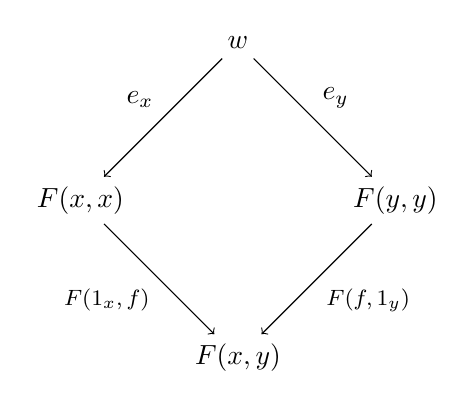
\begin{tikzpicture}
                \node (W) at (0, 4) {$w$};
                \node (F1) at (-2, 2) {$F(x,x)$};
                \node (F2) at (2, 2) {$F(y,y)$};
                \node (F) at (0, 0) {$F(x,y)$};
                \draw[->] (W) edge node[above left]{$e_x$} (F1) (F1) edge node[below left]{\footnotesize$F(\mathbbm{1}_x,f)$} (F);
                \draw[->] (W) edge node[above right]{$e_{y}$} (F2) (F2) edge node[below right]{\footnotesize$F(f,\mathbbm{1}_{y})$} (F);
            \end{tikzpicture}
        \end{gather*}
        As was the case for cones, this can be reformulated in terms of (di)natural transformations. A wedge $(w,e)$ of a profunctor $\profunc{F}{C}{C}$ is a dinatural transformation from the constant profunctor $\Delta_w$ to $F$.
    }
    \newdef{End}{\index{end}
        The end of a profunctor $\profunc{F}{C}{C}$ is defined as the universal wedge of $F$. The components of the wedge are called the \textbf{projection maps} of the end. This stems from the fact that for a discrete category the end coincides with the product $\prod_{x\in\ob{C}}F(x,x)$.

        This is equivalent to a definition in terms of equalizers. Consider the two canonical maps
        \begin{gather}
            \prod_{x\in\ob{C}}\symbfsf{C}(x,x)\rightrightarrows\prod_{f:x\rightarrow y}\symbfsf{C}(x,y)\,.
        \end{gather}
        This diagram can be interpreted as the product of all lower halves of the wedge diagrams above. It is not hard to see that its equalizer (universally) satisfies the wedge condition for all $f\in\mathrm{hom}(\symbfsf{C})$.
    }
    \newnot{End}{
        The end of a profunctor $\profunc{F}{C}{C}$ is often denoted using an integral sign with subscript: \[\int_{x\in\symbfsf{C}}F(x,x)\,.\] For the dual construction, called a \textbf{coend}, an integral sign with superscript is used.
    }
    \begin{example}[Natural transformations]\index{natural!transformation}
        Consider two functors $\func{F,G}{C}{D}$. The map $(x,y)\mapsto\symbfsf{D}(Fx,Gy)$ gives a profunctor $\profunc{H}{C}{C}$. By looking at the wedge condition for this profunctor, the following equality for all morphisms $f:x\rightarrow y$ can be derived:
        \begin{gather}
            \tau_y\circ Ff = Gf\circ\tau_x\,,
        \end{gather}
        where $\tau$ is the wedge projection. Comparing this equality to \cref{cat:natural} gives
        \begin{gather}
            \label{cat:natural_end}
            \mathrm{Nat}(F,G) = \int_{x\in\symbfsf{C}}\symbfsf{D}(Fx,Gx)\,.
        \end{gather}
    \end{example}

    \begin{property}
        Using the continuity of the hom-functor (\cref{cat:continuity}), one can prove the following equality which can be used to turn ends into coends and vice versa:
        \begin{gather}
            \symbfsf{Set}\left(\int^{x\in\symbfsf{C}}F(x,x),y\right) = \int_{x\in\symbfsf{C}}\symbfsf{Set}\left(F(x,x),y\right)\,.
        \end{gather}
    \end{property}

    Using the above properties and definitions, one obtains the following two statements, called the \textbf{Yoneda reduction} and \textbf{co-Yoneda lemma}:
    \begin{property}[Ninja Yoneda lemma]\index{Yoneda!reduction}\index{co-!Yoneda|see{Yoneda, reduction}}\label{cat:ninja_yoneda}
        Let $\func{F}{C}{Set}$ be a covariant functor (similar statements hold for contravariant functors).
        \begin{align}
            &\int_{x\in\symbfsf{C}}\symbfsf{Set}\bigl(\symbfsf{C}(-,x),Fx\bigr)\cong F\\
            &\int^{x\in\symbfsf{C}}\symbfsf{C}(x,-)\times Fx\cong F
        \end{align}
        For a generalization to the enriched setting see \cref{cat:enriched_ninja_yoneda}.
    \end{property}
    \begin{remark}
        A common remark at this point is the comparison with the Dirac distribution~\eqref{distribution:sieving_dirac_delta}:
        \begin{gather}
            \int \delta(x-y)f(x) = f(y)\,.
        \end{gather}
        By interpreting the functor $F$ as a function, the representable functors can be seen to behave as Dirac distributions.
    \end{remark}

    \begin{property}
        \begin{gather}
            \int_{F\in\symbfsf{coPsh}(\symbfsf{C})}\symbfsf{Set}(Fx,Fy)\cong\symbfsf{C}(x,y)
        \end{gather}
    \end{property}

    \newdef{Kan extension}{\index{Kan!extension}\label{cat:kan_extension}
        Consider two functors $\func{F}{A}{B}$ and $\func{G}{A}{C}$. The right Kan extension of $F$ along $G$ is given by the universal functor $\func{\mathrm{Ran}_GF}{C}{B}$ and natural transformation $\eta:\mathrm{Ran}_GF\circ G\Rightarrow F$:
        \begin{gather*}
            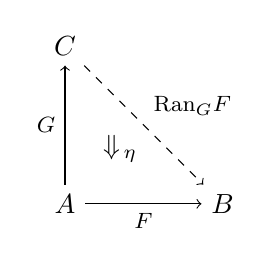
\begin{tikzpicture}
                \node (A) at (0, 0) {$\symbfsf{A}$};
                \node (B) at (2, 0) {$\symbfsf{B}$};
                \node (C) at (0, 2) {$\symbfsf{C}$};
                \node at (0.7, 0.7) {$\Downarrow_{\,\eta}$};
                \draw[->] (A) -- node[left]{\footnotesize$G$} (C);
                \draw[->] (A) -- node[below]{\footnotesize$F$} (B);
                \draw[dashed, ->] (C) -- node[above right]{\footnotesize$\mathrm{Ran}_GF$} (B);
            \end{tikzpicture}
        \end{gather*}
        The left Kan extension $\mathrm{Lan}_GF$ is obtained by dualizing this construction.
    }

    \begin{property}[Complete categories]
        Complete (resp.~cocomplete) categories admit all right (resp.~left) Kan extensions.
    \end{property}

    \newdef{Preservation of Kan extension}{\label{cat:preservation_kan_extension}
        A Kan extension $\mathrm{Lan}_GF$ is said to be \textbf{absolute} if every functor with the same codomain as preserves the Kan extension, i.e.~a Kan extension is absolute if right whiskering it by another functor defines the Kan extension of the composition. If it is only preserved by all representable functors, the Kan extension is said to be \textbf{pointwise} or \textbf{strong}. Pointwise Kan extensions can be expressed as (co)limits, an expression is provided in \cref{cat:enriched_kan_extension} in the \textit{enriched setting} using (co)ends.
    }

    \newadef{Kan extension}{\label{cat:kan_extension_alternative}
        The definition above gives a natural isomorphism (here given for left extension):
        \begin{gather}
            \funccat{A}{B}(F,G^*-)\cong\funccat{C}{B}(\mathrm{Lan}_GF,-)\,.
        \end{gather}
        In the spirit of partial adjoints or partial limits, this construction defines so-called \textbf{local Kan extensions}. If local Kan extensions exist for all functors $F\in\funccat{A}{B}$, a right adjoint $\mathrm{Ran}_G:\funccat{A}{B}\rightarrow\funccat{C}{B}$ to the pullback functor $G^*:F\mapsto F\circ G$ is obtained. Similarly, left Kan extension can be defined as the left adjoint to the pullback functor.
    }
    \remark{Using this equivalence of hom-spaces, Kan extensions can be generalized from $\symbfsf{Cat}$ to any \textit{2-category}.}

    \begin{example}[Limit]\index{limit}
        Denote the terminal category by $\symbfsf{1}$. By choosing the functor $G$ in the definition of a right Kan extension to be the unique functor $!_{\symbfsf{C}}:\symbfsf{C}\rightarrow\symbfsf{1}$, one obtain the universal property characterizing limits (\cref{cat:limit_uproperty}):
        \begin{gather}
            \lim F\cong\mathrm{Ran}_{!_C}F\,.
        \end{gather}
        Similarly, colimits can be obtained as left Kan extensions.
    \end{example}

    The existence of Kan extensions can also be used to determine the existence of adjoints.
    \begin{property}[Adjoint functors]
        A functor $\func{F}{C}{D}$ admits a left (resp.~right) adjoint if and only if the right (resp.~left) Kan extension of the identity functor $\mathbbm{1}_{\symbfsf{C}}$ along $F$ exists. If it exists as an absolute extension, the left adjoint is given exactly by this Kan extension.
    \end{property}

    \newdef{Codensity monad}{\index{monad!codensity}\index{co-!dense}
        Consider a general functor $\func{F}{C}{D}$. If the right Kan extension $\mathrm{Ran}_FF$ exists, it defines a monad. Functors for which this monad is the identity are said to be \textbf{codense}.\footnote{Codense functors are usually defined in a different way, but one can show that this is an equivalent definition (hence the name).} Left Kan extensions give, by duality, rise to \textit{density comonads}.
    }

    \begin{property}[Faithfulness]
        Kan extension along a fully faithful functor is itself a fully faithful functor.
    \end{property}
    \begin{property}[Representability]
        (Left) Kan extension of a representable along a functor $F$ is equivalent to the representable of the image of $F$.
    \end{property}

    \begin{property}[Adjoint quadruple]\label{cat:kan_quadruple}
        Consider an adjunction $F\dashv G$ and consider Kan extension of presheaves taking values in a bicomplete category. In this case precomposition with (the opposite of) one of the adjoints coincides with Kan extension along (the opposite) of the other:
        \begin{align}
            (F^{\text{op}})^* &\cong \mathrm{Lan}_{G^{\text{op}}}\,,\\
            (G^{\text{op}})^* &\cong \mathrm{Ran}_{F^{\text{op}}}\,.
        \end{align}
        This implies that every adjunction induces an adjoint quadruple
        \begin{gather}
            \mathrm{Lan}_{F^{\text{op}}}\dashv\mathrm{Lan}_{G^{\text{op}}}\dashv\mathrm{Ran}_{F^{\text{op}}}\dashv\mathrm{Ran}_{G^{\text{op}}}\,.
        \end{gather}
    \end{property}

\section{Internal structures}\index{internal}\label{section:internal_category_theory}

    \begin{property}[Eckmann--Hilton argument]\index{Eckmann--Hilton!argument}\label{cat:eckmann_hilton}
        A monoid internal to $\symbfsf{Mon}$, the category of monoids, is the same as a commutative monoid. (See also \cref{algebra:eckmann_hilton}.)
    \end{property}

    \newdef{Internal category}{\label{cat:internal_category}
        Let $\mathcal{E}$ be a category with pullbacks. A category $\symbfsf{C}$ internal to $\mathcal{E}$ consists of the following data:
        \begin{itemize}
            \item an object $C_0\in\ob{\mathcal{E}}$ of objects;
            \item an object $C_1\in\ob{\mathcal{E}}$ of morphisms;
            \item source and target morphisms $s, t\in\mathcal{E}(C_1,C_0)$;
            \item an `identity-assigning' morphism $e\in\mathcal{E}(C_0, C_1)$ such that
            \begin{gather}
                s\circ e = \mathbbm{1}_{C_0}\qquad\qquad\qquad t\circ e = \mathbbm{1}_{C_0}\,;
            \end{gather}
            and
            \item a composition morphism $c:C_1\times_{C_0}C_1\rightarrow C_1$ such that the following equations hold:
            \begin{gather}
                \begin{aligned}
                    s\circ c = s\circ\pi_1\qquad\qquad&\qquad\qquad t\circ c = t\circ\pi_2\\
                    \pi_1 = c\circ(e\times_{C_0}\mathbbm{1})\qquad\qquad&\qquad\qquad c\circ(\mathbbm{1}\times_{C_0}e)=\pi_2\\
                    c\circ(c\times_{C_0}\mathbbm{1}) &= c\circ(\mathbbm{1}\times_{C_0}c)\,,
                \end{aligned}
            \end{gather}
            where $\pi_1,\pi_2$ are the canonical projections associated with the pullback $C_1\times_{C_0}C_1$ of $(s,t)$.
        \end{itemize}

        Morphisms between these categories, suitably called \textbf{internal functors}, are given by a pair of morphisms (in $\mathcal{E}$) between internal objects and morphisms, that preserve composition and identities. Internal natural transformations are defined in a similar way.
    }
    \begin{notation}
        The \textit{(bi)category} of internal categories in $\mathcal{E}$ is denoted by $\symbfsf{Cat}(\mathcal{E})$. It should be noted that for $\mathcal{E}=\symbfsf{Set}$, the ordinary category of small categories $\symbfsf{Cat}(\symbfsf{Set})=\symbfsf{Cat}$ is obtained.
    \end{notation}
    \begin{adefinition}
        The above definition can be reformulated in a very elegant way. An internal category in $\mathcal{E}$ is a monad in the bicategory $\symbfsf{Span}(\mathcal{E})$ as shown in \cref{fig:internal_cat_monad}.

        \begin{figure}[ht!]
            \centering
            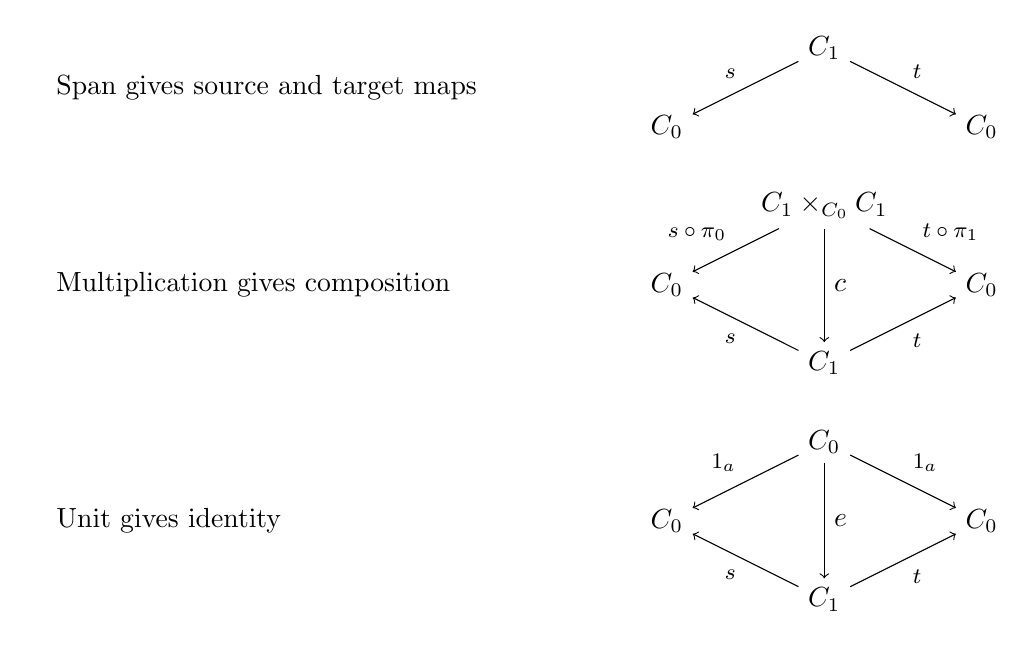
\begin{tikzpicture}
                \node[label={[align=left]right:Span gives source and target maps}] at (-10, -0.5) {};
                \node[label={[align=left]right:Multiplication gives composition}] at (-10, -3) {};
                \node[label={[align=left]right:Unit gives identity}] at (-10, -6) {};
                \node (mor) at (0, 0) {$C_1$};
                \node (ob1) at (-2, -1) {$C_0$};
                \node (ob2) at (2, -1) {$C_0$};
                \draw[->] (mor) -- node[above left]{\footnotesize$s$} (ob1);
                \draw[->] (mor) -- node[above right]{\footnotesize$t$} (ob2);
                \node (MM) at (0, -2) {$C_1\times_{C_0}C_1$};
                \node (M1) at (0, -4) {$C_1$};
                \node (O1) at (-2, -3) {$C_0$};
                \node (O2) at (2, -3) {$C_0$};
                \draw[->] (MM) -- node[above left]{\footnotesize$s\circ\pi_0$} (O1);
                \draw[->] (MM) -- node[above right]{\footnotesize$t\circ\pi_1$} (O2);
                \draw[->] (MM) -- node[right]{$c$} (M1);
                \draw[->] (M1) -- node[below left]{\footnotesize$s$} (O1);
                \draw[->] (M1) -- node[below right]{\footnotesize$t$} (O2);
                \node (O3) at (0, -5) {$C_0$};
                \node (M2) at (0, -7) {$C_1$};
                \node (O4) at (-2, -6) {$C_0$};
                \node (O5) at (2, -6) {$C_0$};
                \draw[->] (O3) -- node[above left]{\footnotesize$\mathbbm{1}_a$} (O4);
                \draw[->] (O3) -- node[above right]{\footnotesize$\mathbbm{1}_a$} (O5);
                \draw[->] (O3) -- node[right]{$e$} (M2);
                \draw[->] (M2) -- node[below left]{\footnotesize$s$} (O4);
                \draw[->] (M2) -- node[below right]{\footnotesize$t$} (O5);
            \end{tikzpicture}
            \caption{Internal category as a monad in $\symbfsf{Span}(\mathcal{E})$.}
            \label{fig:internal_cat_monad}
        \end{figure}
    \end{adefinition}

    Functors between internal categories are not the only relevant morphisms. However, when defining (co)presheaves such as the hom-functor, a problem occurs. In $\symbfsf{Cat}$ there exist, by definition, maps to the ambient category $\symbfsf{Set}$ (ordinary category theory has a set-theoretic foundation). However, for internal categories there does not necessarily exist a morphism $\symbfsf{C}\rightarrow\mathcal{E}$. To solve this problem, one can consider a more general structure.
    \newdef{Internal diagram}{\index{diagram}\label{cat:internal_diagram}
        A left module over a monad in $\symbfsf{Span}(\mathcal{E})$. The dual notion is better known as an \textbf{internal presheaf}. The category of internal diagrams on an internal category $\symbfsf{C}\in\symbfsf{Cat}(\mathcal{E})$ is denoted by $\mathcal{E}^{\symbfsf{C}}$.

        This can be spelled out more explicitly. An internal diagram in an internal category $\symbfsf{C}\in\symbfsf{Cat}(\mathcal{E})$ consists of:
        \begin{enumerate}
            \item a morphism $\gamma_0:F_0\rightarrow C_0$, and
            \item a morphism $\mathrm{ap}:F_0\times_{C_0}C_1\rightarrow F_0$
        \end{enumerate}
        satisfying:
        \begin{gather}
            \begin{aligned}
                \gamma_0\circ\mathrm{ap} &= d_1\circ\pi_{C_1}\\
                \mathrm{ap}\circ(\mathbbm{1}_{F_0}\times e)&=\pi_{F_0}\\
                \mathrm{ap}\circ(\mathrm{ap}\times\mathbbm{1}_{C_0})&=\mathrm{ap}\circ(\mathbbm{1}_{F_0}\times c)
            \end{aligned}
        \end{gather}
    }
    \newadef{Internal diagram}{
        An object of the slice category $\symbfsf{Cat}(\mathcal{E})_{/\symbfsf{C}}$ satisfying the following pullback condition:
        \begin{gather}
            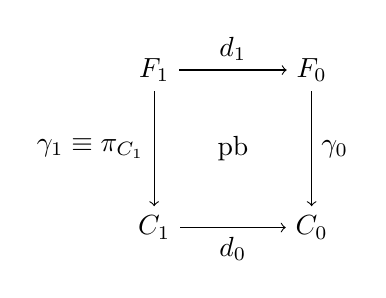
\begin{tikzpicture}[baseline=(current bounding box.center)]
                \node (F1) at (0, 0) {$F_1$};
                \node (C1) at (0, -2) {$C_1$};
                \node (F0) at (2, 0) {$F_0$};
                \node (C0) at (2, -2) {$C_0$};
                \node at (1, -1) {pb};
                \draw[->] (F1) -- node[left]{$\gamma_1\equiv\pi_{C_1}$} (C1);
                \draw[->] (F1) -- node[above]{$d_1$} (F0);
                \draw[->] (F0) -- node[right]{$\gamma_0$} (C0);
                \draw[->] (C1) -- node[below]{$d_0$} (C0);
            \end{tikzpicture}
        \end{gather}
    }

    In fact, this is a specific instance of an even more general concept. For more information on the definitions and applications, see~\citet{mac_lane_categories_2013, johnstone_topos_2014}.
    \newdef{Internal profunctor}{\index{pro-!functor}
        A bimodule between monads in $\symbfsf{Span}(\mathcal{E})$. Together with the above definitions, this gives rise to an equivalence
        \begin{gather}
            \symbfsf{Mod}(\symbfsf{Span}(\mathcal{E}))\cong\symbfsf{Prof}(\mathcal{E})\,.
        \end{gather}
    }

    \begin{construct}[Internal Yoneda profunctor]
        Consider an internal functor $\func{F}{C}{D}$. This functor induces two internal profunctors $\profunc{F_*}{D}{C}$ and $\profunc{F^*}{C}{D}$. For $F_*$ (the profunctor $F^*$ is defined similarly) the object span is defined as
        \begin{gather}
            C_0\overset{\pi_0}{\longleftarrow}C_0\times_{D_0} D_1\overset{t\circ\pi_1}{\longrightarrow}D_0\,.
        \end{gather}
        The action of $f\in D_1$ is given by postcomposition with $f$ in the second factor, while the action of $g\in C_1$ is given by precomposition with $Fg$ in the second factor and changing to the domain of $g$ in the first factor.

        It can easily be shown that the profunctors induced by an identity functor $\mathbbm{1}_{\symbfsf{C}}$ have an object span that corresponds to the internal category $\symbfsf{C}$ with the actions given by (internal) composition. In the case of $\mathcal{E}=\symbfsf{Set}$, this boils down to the hom-functor. The fact that the object span is equivalent to the category $\symbfsf{C}$ is essentially the Yoneda embedding. For this reason, this profunctor is in general called the (internal) Yoneda profunctor $\mathcal{Y}(\symbfsf{C})$.
    \end{construct}

\subsection{Groupoids}\label{section:groupoids}

    \newdef{Groupoid}{\index{groupoid}\label{cat:groupoid}
        A (small) groupoid $\mathcal{G}$ is a (small) category in which all morphisms are invertible.
    }

    \begin{example}[Action groupoid]\index{groupoid!action}\label{cat:action_groupoid}
        Consider a set $X$ with an action of a group $G$. The action groupoid $X/\!\!/G$ is defined as the following category:
        \begin{enumerate}
            \item\textbf{Objects}: $X$,
            \item\textbf{Morphisms}: An arrow $x\rightarrow y$ for every $g\in G$ such that $g\cdot x=y$.
        \end{enumerate}
    \end{example}

    \begin{example}[Delooping]\index{delooping!of groups}\label{cat:group_delooping}
        Consider a group $G$. Its delooping $\symbfsf{B}G$ is defined as the one-object groupoid for which $\symbfsf{B}G(\ast,\ast)=G$.
    \end{example}
    \begin{property}[Representations]\label{cat:delooping_representation}
        Consider a group $G$ together with its delooping $\symbfsf{B}G$. When considering \textit{representations} as functors $\rho:\symbfsf{B}G\rightarrow\symbfsf{FinVect}$, one can see that the intertwiners (\cref{group:equivariant}) are exactly the natural transformations. More generally, all $G$-sets (\cref{group:group_action}) can be obtained as functors $\symbfsf{B}G\rightarrow\symbfsf{Set}$.
    \end{property}

    \newdef{Core}{\index{core}\label{cat:core}
        Let $\symbfsf{C}$ be a (small) category. The core $\mathrm{Core}(\symbfsf{C})\in\symbfsf{Grpd}$ of $\symbfsf{C}$ is defined as the maximal subgroupoid of $\symbfsf{C}$.
    }

    \newdef{Orbit}{\index{orbit}
        Let $\mathcal{G}$ be a groupoid with $O,M$ respectively the sets of objects and morphisms. On $O$ one can define an equivalence $x\sim y\iff\exists\phi:x\rightarrow y$. The equivalence classes are called orbits and the set of orbits is denoted by $O/M$.
    }
    \newdef{Transitive component}{\index{transitive!component}
        Let $\mathcal{G}$ be a groupoid with $O,M$ respectively the sets of objects and morphisms and let $s,t$ denote the source and target maps on $M$. Given an orbit $o\in O/M$, the transitive component of $M$ associated to $o$ is defined as $s^{-1}(o)$, or equivalently, as $t^{-1}(o)$.
    }
    \begin{property}
        Every groupoid is a (disjoint) union of its transitive components.
    \end{property}
    \newdef{Transitive groupoid}{\index{transitive!groupoid}
        A groupoid $\mathcal{G}$ is said to be transitive if for all objects $x\neq y\in\ob{\mathcal{G}}$, the set $\mathcal{G}(x,y)$ is not empty.
    }

\section{\difficult{Lawvere theories}}

    \newdef{Lawvere theory}{\index{Lawvere!theory}
        Let $\symbfsf{F}$ denote the skeleton of $\symbfsf{FinSet}$. A Lawvere theory consists of a small category $\symbfsf{L}$ and a strict (finite) product-preserving \textit{identity-on-objects} functor $\mathcal{L}:\symbfsf{F}^{\text{op}}\rightarrow\symbfsf{L}$.

        Equivalently, a Lawvere theory is a small category $\symbfsf{L}$ with a \textbf{generic object} $c_0$ such that every object $c\in\ob{L}$ is a finite power of $c_0$.
    }
    \begin{property}
        Lawvere theories $(\symbfsf{L},\mathcal{L})$ form a category $\symbfsf{Law}$. Morphisms between Lawvere theories are (finite) product-preserving functors.
    \end{property}

    \newdef{Model}{\index{model}\index{algebra}
        A model or \textbf{algebra} over a Lawvere theory $\symbfsf{L}$ is a (finite) product-preserving functor $\func{A}{L}{Set}$.
    }

\section{\difficult{Operad theory}}
\subsection{Operads}

    \newdef{Plain operad\footnotemark}{\index{operad}\index{arity}
        \footnotetext{Also called a \textbf{nonsymmetric operad} or \textbf{non-$\Sigma$ operad}.}
        Let $\mathcal{O}=\{P(n)\}_{n\in\mathbb{N}}$ be a collection of sets, called \textbf{$n$-ary operations} (where $n$ is called the \textbf{arity}). The collection $\mathcal{O}$ is called a plain operad if it satisfies following axioms:
        \begin{enumerate}
            \item $P(1)$ contains an identity element $\mathbbm{1}$.
            \item For all positive integers $n,k_1,\ldots,k_n$ there exists a composition map
            \begin{align}
                \circ&:P(n)\times P(k_1)\times\cdots\times P(k_n)\rightarrow P(k_1+\cdots+k_n)\nonumber\\
                &:(\psi,\theta_1,\ldots,\theta_n)\mapsto \psi\circ(\theta_1,\ldots,\theta_n)
            \end{align}
            that satisfies two additional axioms:
            \begin{itemize}
                \item\textbf{identity}:
                \begin{gather}
                    \theta\circ (\mathbbm{1},\ldots,\mathbbm{1}) = \mathbbm{1}\circ\theta = \theta,
                \end{gather}
                and
                \item\textbf{associativity}:
                \begin{align}
                    \psi\circ\Bigl(\theta_1\,\circ\,&(\theta_{1,1},\ldots,\theta_{1,k_1}),\ldots,\theta_n\circ(\theta_{n,1},\ldots,\theta_{n,k_n})\Big)\nonumber\\
                    &= \Bigr(\psi\circ(\theta_1,\ldots,\theta_n)\Big) \circ (\theta_{1,1},\ldots,\theta_{1,k_1},\theta_{2,1},\ldots,\theta_{n,k_n}).
                \end{align}
            \end{itemize}
        \end{enumerate}
        If the operad is represented using planar tree diagrams, the associativity obtains a nice intuitive form. When combining planar tree diagrams in three layers, the associativity axiom says that one can either first glue the first two layers together or one can first glue the last two layers together.
    }
    \remark{Plain operads can be defined in any monoidal category. In the same way symmetric operad can be defined in any symmetric monoidal category.}

    \begin{example}[Endomorphism operad]\index{endo-!morphism operad}
        Consider a vector space $V$. For every $n\in\mathbb{N}$, one can define the endomorphism algebra $\End(V^{\otimes n}, V)$. The endomorphism operad $\mathcal{E}\text{nd}(V)$ is defined as $\{\End(V^{\otimes n},V)\}_{n\in\mathbb{N}}$.
    \end{example}

    \newdef{$O$-algebra}{\index{algebra!over an operad}
        An object $X$ is called an algebra over an operad $O$ if there exist morphisms \[O(n)\times X^n\rightarrow X\] for every $n\in\mathbb{N}$ satisfying the usual composition and identity laws. Alternatively, this can be rephrased as the existence of a (plain) operad morphism $O(n)\rightarrow\mathcal{E}\text{nd}(X)$.
    }
    \begin{example}[Categorical $O$-algebra]
        An $O$-algebra in the category $\symbfsf{Cat}$.
    \end{example}

\subsection{Algebraic topology}

    \newdef{Stasheff operad}{\index{Stasheff!operad}
        A topological operad $\mathcal{K}$ such that $\mathcal{K}(n)$ is given by the $n^{\text{th}}$ \textit{Stasheff polytope/associahedron}. Composition is given by the inclusion of faces.
    }
    \newdef{$A_\infty$-space}{\index{A${}_\infty$-space}\label{cat:A_infinity_space}
        An algebra over the Stasheff operad. This induces the structure of a multiplication that is associative up to a coherent homotopy.
    }

    \newdef{Little $k$-cubes operad}{\index{operad!little $k$-cubes}
        A topological operad for which every topological space $\mathcal{P}(n)$ consists of all possible configurations of $n$ embedded $k$-cubes in a (unit) $k$-cube. Composition is given by the obvious way of inserting one unit $k$-cube in one of the smaller embedded $k$-cubes.
    }
    \begin{property}[Recognition principle]\index{recognition principle}
        If a connected topological space $X$ forms an algebra over the little $k$-cubes operad, it is (weakly) homotopy equivalent to the $k$-fold loop space $\Omega^kY$ of another pointed topological space $Y$. For $k=1$, one should technically use the Stasheff operad, but it can be shown that this is related to the little interval operad.
    \end{property}
% \chapter{\difficult{Higher-dimensional Algebra}}\label{chapter:hda}

    The main reference for this chapter is the series of papers carrying the same name by~\citet{baez_higher-dimensional_2003, baez_higher-dimensional_2003-1}. References for the section on Berezin calculus are~\citet{losev_berezin_2007, choquet-bruhat_analysis_2000}. For Kapranov-Voevodsky 2-vector spaces the reader is referred to the original paper~\citet{kapranov_2-categories_1994}. The section about higher Lie theory is mainly based on~\citet{fiorenza_introduction_2004}. For fusion and modular categories, the main reference is~\citet{etingof_tensor_2016}.

\section{Monoidal categories}\label{section:monoidal_categories}

    \newdef{Monoidal category}{\index{monoidal!category}\index{tensor product}\label{cat:monoidal_category}
        A category $\mathbf{C}$ equipped with a bifunctor
        \begin{gather}
            -\otimes -:\mathbf{C}\times\mathbf{C}\rightarrow\mathbf{C}
        \end{gather}
        called the \textbf{tensor product} or \textbf{monoidal product}, a distinct object $\mathbf{1}$ called the \textbf{(monoidal) unit}, and the following three natural isomorphisms called the \textbf{coherence maps}:
        \begin{itemize}
            \item\textbf{Associator}: $\alpha_{x,y,z}:(x\otimes y)\otimes z\cong x\otimes(y\otimes z)$;
            \item\textbf{Left unitor}: $\lambda_x:\mathbf{1}\otimes x\cong x$; and
            \item\textbf{Right unitor}: $\rho_x:x\otimes\mathbf{1}\cong x$.
        \end{itemize}
        These natural transformations are required make the \textbf{triangle} and \textbf{pentagon} diagrams~\ref{fig:triangle_diagram} and~\ref{fig:pentagon_diagram} commute.

        \begin{figure}[ht!]
            \centering
            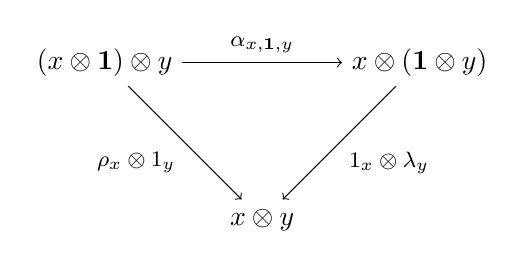
\begin{tikzpicture}
                \node (1) at (0, 0) {$(x\otimes\mathbf{1})\otimes y$};
                \node (2) at (4, 0) {$x\otimes(\mathbf{1}\otimes y)$};
                \node (3) at (2, -2) {$x\otimes y$};
                \draw[->] (1) -- node[above]{\footnotesize$\alpha_{x,\mathbf{1},y}$} (2);
                \draw[->] (1) -- node[below left]{\footnotesize$\rho_x\otimes\mathbbm{1}_y$} (3);
                \draw[->] (2) -- node[below right]{\footnotesize$\mathbbm{1}_x\otimes\lambda_y$} (3);
            \end{tikzpicture}
            \caption{Triangle diagram.}
            \label{fig:triangle_diagram}
        \end{figure}
        \begin{figure}[ht!]
            \centering
            \begin{tikzpicture}
                \node (1) at (0, 0) {$((w\otimes x)\otimes y)\otimes z$};
                \node (2) at (6, 0) {$(w\otimes(x\otimes y))\otimes z$};
                \node (3) at (-2, -3) {$(w\otimes x)\otimes(y\otimes z)$};
                \node (4) at (8, -3) {$w\otimes((x\otimes y)\otimes z)$};
                \node (5) at (3, -6) {$w\otimes(x\otimes(y\otimes z))$};
                \draw[->] (1) -- node[above]{\small$\alpha_{w,x,y}\otimes\mathbbm{1}_z$} (2);
                \draw[->] (1) -- node[above left]{\small$\alpha_{w\otimes x,y,z}$} (3);
                \draw[->] (3) -- node[below left]{\small$\alpha_{w,x,y\otimes z}$} (5);
                \draw[->] (2) -- node[above right]{\small$\alpha_{w,x\otimes y,z}$} (4);
                \draw[->] (4) -- node[below right]{\small$\mathbbm{1}_w\otimes\alpha_{x,y,z}$} (5);
            \end{tikzpicture}
            \caption{Pentagon diagram.}
            \label{fig:pentagon_diagram}
        \end{figure}
        A monoidal category for which the associator and the unitors are identity transformations is often said to be \textbf{strict}.
    }

    \begin{example}[Cartesian category]\label{cat:semicartesian}
        A monoidal category where the monoidal product is given by the ordinary product (\cref{cat:product}). If the monoidal product is not the ordinary product, but the monoidal unit is still terminal, the category is said to be \textbf{semicartesian}.
    \end{example}

    \newdef{Scalar}{\index{scalar}
        In a monoidal category the scalars are defined as the endomorphisms $\mathbf{1}\rightarrow\mathbf{1}$. The set of scalars forms a commutative monoid.
    }
    \begin{property}
        Every scalar $s:\mathbf{1}\rightarrow\mathbf{1}$ induces a natural transformation $s:\mathbbm{1}_{\mathbf{C}}\Rightarrow\mathbbm{1}_{\mathbf{C}}$ with components
        \begin{gather}
            s_x:x\cong\mathbf{1}\otimes x\overset{s\otimes\mathbbm{1}_x}{\longrightarrow}\mathbf{1}\otimes x\cong x\,.
        \end{gather}
        For every morphism $f\in\mathrm{hom}(\mathbf{C})$, the naturality square $f\circ s_x=s_y\circ f$ alo defines a morphism $s\diamond f$ that is equivalently given by $\rho_y\circ(f\otimes s)\circ\rho^{-1}_x$ (one could have used the left unitors as well). These morphisms satisfy the following well-known rules of scalar multiplication from linear algebra:
        \begin{itemize}
            \item $s\diamond(s'\diamond f) = (s\circ s')\diamond f$,
            \item $(s\diamond f)\circ(s'\diamond g) = (s\circ s')\diamond(f\circ g)$, and
            \item $(s\diamond f)\otimes(s'\diamond g) = (s\circ s')\diamond(f\otimes g)$.
        \end{itemize}
    \end{property}

    \newdef{Weak inverse}{\index{weak!inverse}
        Let $(\mathbf{C},\otimes,\mathbf{1})$ be a monoidal category and consider an object $x\in\ob{C}$. An object $y\in\ob{C}$ is called a weak inverse of $x$ if it satisfies $x\otimes y\cong\mathbf{1}$.
    }
    \remark{One can show that the existence of a one-sided weak inverse (as in the definition above) is sufficient to prove that it is in fact a two-sided weak inverse, i.e.~$y\otimes x\cong\mathbf{1}$ also holds.}

    \begin{theorem}[MacLane's coherence theorem]\index{coherence!theorem}
        Consider two functors $\func{F,G}{A}{B}$ between two monoidal categories $\mathbf{A},\mathbf{B}$. Any two natural transformations $\eta,\varepsilon:F\Rightarrow G$, constructed solely from the associator and the unitors, coincide.
    \end{theorem}

\subsection{Braided categories}

    \newdef{Braided monoidal category}{\index{braiding}
        A monoidal category $(\mathbf{C},\otimes,\mathbf{1})$ equipped with a natural isomorphism
        \begin{gather}
            \sigma_{x,y}:x\otimes y\cong y\otimes x
        \end{gather}
        that makes the two \textbf{hexagon} diagrams~\ref{fig:hexagon_diagrams1} and~\ref{fig:hexagon_diagrams2} commute for all $x,y,z\in\ob{C}$. The isomorphism $\sigma$ is called the \textbf{braiding} (morphism).
        \begin{figure}[ht!]
            \centering
            \begin{subfigure}[b]{0.49\textwidth}
                \centering
                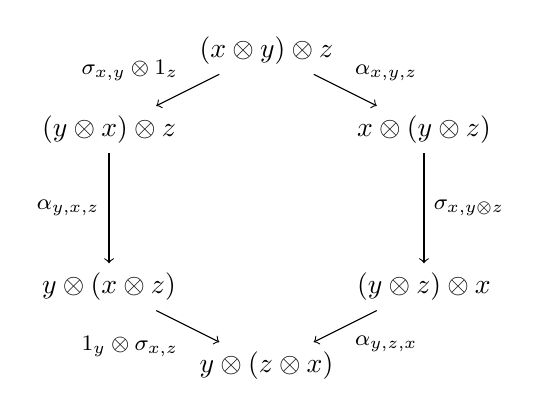
\begin{tikzpicture}
                    \node (1) at (0, 0) {$(x\otimes y)\otimes z$};
                    \node (2) at (-2, -1) {$(y\otimes x)\otimes z$};
                    \node (3) at (2, -1) {$x\otimes(y\otimes z)$};
                    \node (4) at (-2, -3) {$y\otimes(x\otimes z)$};
                    \node (5) at (2, -3) {$(y\otimes z)\otimes x$};
                    \node (6) at (0, -4) {$y\otimes(z\otimes x)$};
                    \draw[->] (1) -- node[above left]{\footnotesize$\sigma_{x,y}\otimes\mathbbm{1}_z$} (2);
                    \draw[->] (1) -- node[above right]{\footnotesize$\alpha_{x,y,z}$} (3);
                    \draw[->] (2) -- node[left]{\footnotesize$\alpha_{y,x,z}$} (4);
                    \draw[->] (3) -- node[right]{\footnotesize$\sigma_{x,y\otimes z}$} (5);
                    \draw[->] (4) -- node[below left]{\footnotesize$\mathbbm{1}_y\otimes\sigma_{x,z}$} (6);
                    \draw[->] (5) -- node[below right]{\footnotesize$\alpha_{y,z,x}$} (6);
                \end{tikzpicture}
                \caption{Hexagon diagram 1.}
                \label{fig:hexagon_diagrams1}
            \end{subfigure}
            \begin{subfigure}[b]{0.49\textwidth}
                \centering
                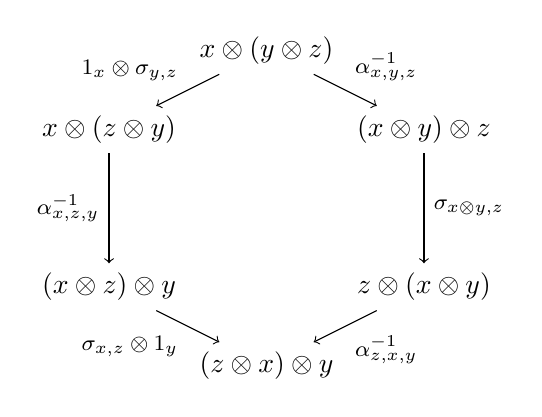
\begin{tikzpicture}
                    \node (1) at (0, 0) {$x\otimes(y\otimes z)$};
                    \node (2) at (-2, -1) {$x\otimes(z\otimes y)$};
                    \node (3) at (2, -1) {$(x\otimes y)\otimes z$};
                    \node (4) at (-2, -3) {$(x\otimes z)\otimes y$};
                    \node (5) at (2, -3) {$z\otimes(x\otimes y)$};
                    \node (6) at (0, -4) {$(z\otimes x)\otimes y$};
                    \draw[->] (1) -- node[above left]{\footnotesize$\mathbbm{1}_x\otimes\sigma_{y,z}$} (2);
                    \draw[->] (1) -- node[above right]{\footnotesize$\alpha^{-1}_{x,y,z}$} (3);
                    \draw[->] (2) -- node[left]{\footnotesize$\alpha^{-1}_{x,z,y}$} (4);
                    \draw[->] (3) -- node[right]{\footnotesize$\sigma_{x\otimes y,z}$} (5);
                    \draw[->] (4) -- node[below left]{\footnotesize$\sigma_{x,z}\otimes\mathbbm{1}_y$} (6);
                    \draw[->] (5) -- node[below right]{\footnotesize$\alpha^{-1}_{z,x,y}$} (6);
                \end{tikzpicture}
                \caption{Hexagon diagram 2.}
                \label{fig:hexagon_diagrams2}
            \end{subfigure}
            \caption{Hexagon diagram.}
            \label{fig:hexagon_diagrams}
        \end{figure}
    }
    \begin{property}[Yang--Baxter equation]\index{Yang--Baxter}
        The components $\sigma_{x,x}$ of a braiding satisfy the \textit{Yang--Baxter equation}. More generally, the braiding $\sigma$ satisfies the following equation for all objects $x,y,z\in\ob{C}$:
        \begin{gather}
            (\sigma_{y,z}\otimes\mathbbm{1}_x)\circ(\mathbbm{1}_y\otimes\sigma_{x,z})\circ(\sigma_{x,y}\otimes\mathbbm{1}_z) = (\mathbbm{1}_z\otimes\sigma_{x,y})\circ(\sigma_{x,z}\otimes\mathbbm{1}_y)\circ(\mathbbm{1}_x\otimes\sigma_{y,z})\,.
        \end{gather}
    \end{property}
    \remark{When drawing the above equality using string diagrams, it can be seen that the Yang--Baxter equation corresponds to the invariance of string diagrams under a \textit{Reidemeister III move}.\index{Reidemeister move}}

    \newdef{Symmetric monoidal category}{\label{cat:symmetric}
        A braided monoidal category where the braiding $\sigma$ satisfies
        \begin{gather}
            \sigma_{x,y}\circ\sigma_{y,x} = \mathbbm{1}_{x\otimes y}\,.
        \end{gather}
    }

    In Chapter \ref{chapter:hda} the theory of monoidal categories is continued.

\subsection{Monoidal functors}

    \begin{figure}[ht!]
        \centering
        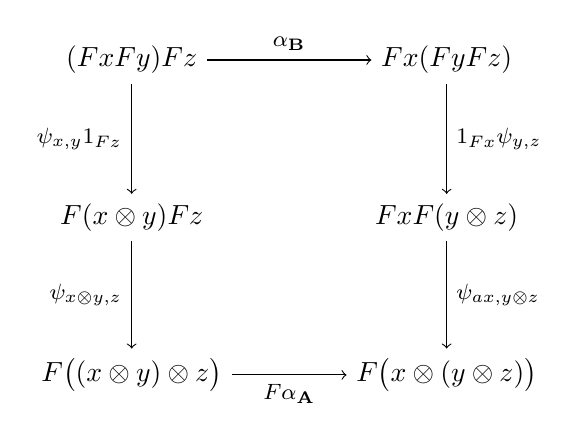
\begin{tikzpicture}
            \node (1) at (0, 0) {$(Fx\circledast Fy)\circledast Fz$};
            \node (2) at (4, 0) {$Fx\circledast(Fy\circledast Fz)$};
            \node (3) at (0, -2) {$F(x\otimes y)\circledast Fz$};
            \node (4) at (4, -2) {$Fx\circledast F(y\otimes z)$};
            \node (5) at (0, -4) {$F\bigl((x\otimes y)\otimes z\bigr)$};
            \node (6) at (4, -4) {$F\bigl(x\otimes(y\otimes z)\bigr)$};
            \draw[->] (1) -- node[above]{\footnotesize$\alpha_{\mathbf{B}}$} (2);
            \draw[->] (5) -- node[below]{\footnotesize$F\alpha_{\mathbf{A}}$} (6);
            \draw[->] (1) -- node[left]{\footnotesize$\psi_{x,y}\circledast\mathbbm{1}_{Fz}$} (3);
            \draw[->] (3) -- node[left]{\footnotesize$\psi_{x\otimes y,z}$} (5);
            \draw[->] (2) -- node[right]{\footnotesize$\mathbbm{1}_{Fx}\circledast\psi_{y,z}$} (4);
            \draw[->] (4) -- node[right]{\footnotesize$\psi_{ax,y\otimes z}$} (6);
        \end{tikzpicture}
        \caption{Monoidal functor.}
        \label{fig:monoidal_functor1}
    \end{figure}

    \newdef{Monoidal functor}{\index{monoidal!functor}\index{coherence!maps}
        Let $(\mathbf{A},\otimes,\mathbf{1}_{\mathbf{A}}),(\mathbf{B},\circledast,\mathbf{1}_{\mathbf{B}})$ be two monoidal categories. A functor $\func{F}{A}{B}$ is said to be monoidal if there exists:
        \begin{enumerate}
            \item A natural isomorphism $\psi_{x,y}:Fx\circledast Fy\Rightarrow F(x\otimes y)$ that makes the diagram in \cref{fig:monoidal_functor1} commute.
            \item An isomorphism $\phi:\mathbf{1}_{\mathbf{B}}\rightarrow F\mathbf{1}_{\mathbf{A}}$ that makes the two diagrams in \cref{fig:unitality} commute.
        \end{enumerate}
    }
    \remark{The maps $\psi$ and $\phi$ are also called \textbf{coherence maps} or \textbf{structure morphisms}.}

    \begin{figure}[ht!]
        \centering
        \begin{subfigure}[b]{0.49\textwidth}
            \centering
            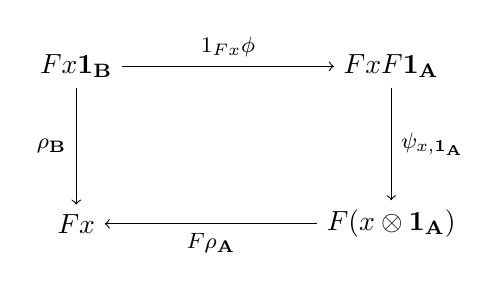
\begin{tikzpicture}
                \node (1) at (0, 0) {$Fx\circledast\mathbf{1}_{\mathbf{B}}$};
                \node (2) at (4, 0) {$Fx\circledast F\mathbf{1}_{\mathbf{A}}$};
                \node (3) at (0, -2) {$Fx$};
                \node (4) at (4, -2) {$F(x\otimes\mathbf{1}_{\mathbf{A}})$};
                \draw[->] (1) -- node[above]{\footnotesize$\mathbbm{1}_{Fx}\circledast\phi$} (2);
                \draw[<-] (3) -- node[below]{\footnotesize$F\rho_{\mathbf{A}}$} (4);
                \draw[->] (1) -- node[left]{\footnotesize$\rho_{\mathbf{B}}$} (3);
                \draw[->] (2) -- node[right]{\footnotesize$\psi_{x,\mathbf{1}_{\mathbf{A}}}$} (4);
            \end{tikzpicture}
        \end{subfigure}
        \begin{subfigure}[b]{0.49\textwidth}
            \centering
            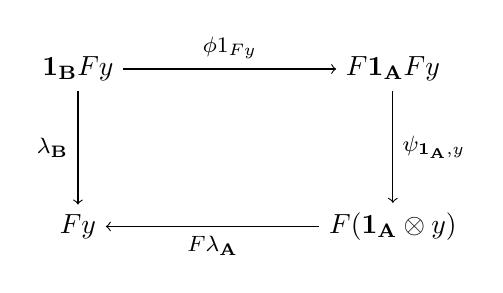
\begin{tikzpicture}
                \node (1) at (0, 0) {$\mathbf{1}_{\mathbf{B}}\circledast Fy$};
                \node (2) at (4, 0) {$F\mathbf{1}_{\mathbf{A}}\circledast Fy$};
                \node (3) at (0, -2) {$Fy$};
                \node (4) at (4, -2) {$F(\mathbf{1}_{\mathbf{A}}\otimes y)$};
                \draw[->] (1) -- node[above]{\footnotesize$\phi\circledast\mathbbm{1}_{Fy}$} (2);
                \draw[<-] (3) -- node[below]{\footnotesize$F\lambda_{\mathbf{A}}$} (4);
                \draw[->] (1) -- node[left]{\footnotesize$\lambda_{\mathbf{B}}$} (3);
                \draw[->] (2) -- node[right]{\footnotesize$\psi_{\mathbf{1}_{\mathbf{A}},y}$} (4);
            \end{tikzpicture}
        \end{subfigure}
        \caption{Unitality diagrams.}
        \label{fig:unitality}
    \end{figure}

    \begin{property}[Canonical unit]
        For every monoidal functor $F$ there exists a canonical isomorphism $\phi:\mathbf{1}_{\mathbf{B}}\rightarrow F\mathbf{1}_{\mathbf{A}}$ defined by the commutative diagram in \cref{fig:canonical_monoidal_isom}.

        \begin{figure}[ht!]
            \centering
            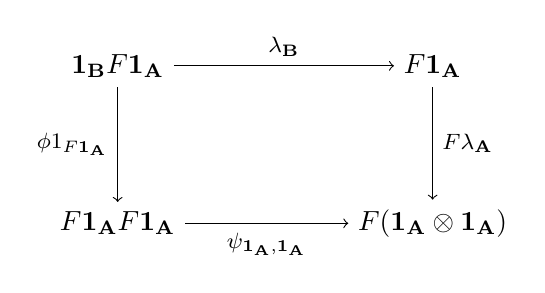
\begin{tikzpicture}
                \node (1) at (0, 0) {$\mathbf{1}_{\mathbf{B}}\circledast F\mathbf{1}_{\mathbf{A}}$};
                \node (2) at (4, 0) {$F\mathbf{1}_{\mathbf{A}}$};
                \node (3) at (0, -2) {$F\mathbf{1}_{\mathbf{A}}\circledast F\mathbf{1}_{\mathbf{A}}$};
                \node (4) at (4, -2) {$F(\mathbf{1}_{\mathbf{A}}\otimes\mathbf{1}_{\mathbf{A}})$};
                \draw[->] (1) -- node[above]{\footnotesize$\lambda_{\mathbf{B}}$} (2);
                \draw[->] (3) -- node[below]{\footnotesize$\psi_{\mathbf{1}_{\mathbf{A}}, \mathbf{1}_{\mathbf{A}}}$} (4);
                \draw[->] (1) -- node[left]{\footnotesize$\phi\circledast\mathbbm{1}_{F\mathbf{1}_{\mathbf{A}}}$} (3);
                \draw[->] (2) -- node[right]{\footnotesize$F\lambda_{\mathbf{A}}$} (4);
            \end{tikzpicture}
            \caption{Canonical unit isomorphism.}
            \label{fig:canonical_monoidal_isom}
        \end{figure}
    \end{property}

    \newdef{Lax monoidal functor}{\index{lax!monoidal functor}
        A monoidal functor for which the coherence maps are merely morphisms and not isomorphisms.
    }

    \newdef{Monoidal natural transformation}{
        A natural transformation $\eta$ between (lax) monoidal functors $(F,\psi,\phi_F)$ and $(G,\widetilde{\psi},\phi_G)$ that makes the diagrams in \cref{fig:monoidal_natural_transformation} commute.
        \begin{figure}[ht!]
            \centering
            \begin{subfigure}[b]{0.49\textwidth}
                \centering
                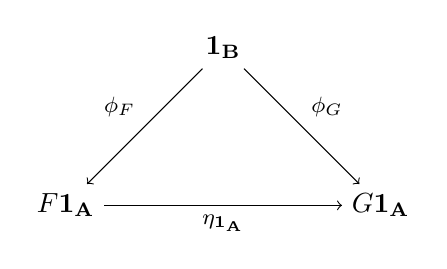
\begin{tikzpicture}
                    \node (1) at (0, 0) {$\mathbf{1}_{\mathbf{B}}$};
                    \node (2) at (-2, -2) {$F\mathbf{1}_{\mathbf{A}}$};
                    \node (3) at (2, -2) {$G\mathbf{1}_{\mathbf{A}}$};
                    \draw[->] (1) -- node[above left]{\footnotesize$\phi_F$} (2);
                    \draw[->] (1) -- node[above right]{\footnotesize$\phi_G$} (3);
                    \draw[->] (2) -- node[below]{\footnotesize$\eta_{\mathbf{1}_{\mathbf{A}}}$} (3);
                \end{tikzpicture}
            \end{subfigure}
            \begin{subfigure}[b]{0.49\textwidth}
                \centering
                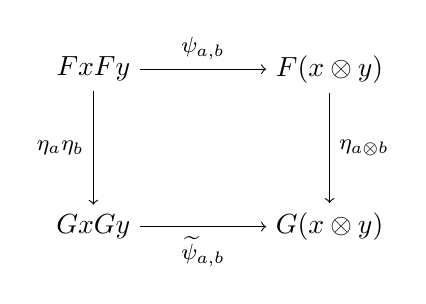
\begin{tikzpicture}
                    \node (1) at (0, 0) {$Fx\circledast Fy$};
                    \node (2) at (3, 0) {$F(x\otimes y)$};
                    \node (3) at (0, -2) {$Gx\circledast Gy$};
                    \node (4) at (3, -2) {$G(x\otimes y)$};
                    \draw[->] (1) -- node[above]{\footnotesize$\psi_{a,b}$} (2);
                    \draw[->] (3) -- node[below]{\footnotesize$\widetilde{\psi}_{a,b}$} (4);
                    \draw[->] (1) -- node[left]{\footnotesize$\eta_a\circledast\eta_b$} (3);
                    \draw[->] (2) -- node[right]{\footnotesize$\eta_{a\otimes b}$} (4);
                \end{tikzpicture}
            \end{subfigure}
            \caption{Monoidal natural transformation.}
            \label{fig:monoidal_natural_transformation}
        \end{figure}
    }

    \newdef{Monoidal equivalence}{\index{monoidal!equivalence}
        An equivalence of monoidal categories consisting of monoidal functors and monoidal natural isomorphisms.
    }
    \begin{theorem}[MacLane's strictness theorem]\index{MacLane!strictness theorem}
        Every monoidal category is monoidally equivalent to a strict monoidal category.
    \end{theorem}

\subsection{Closed categories}

    \newdef{Internal hom}{\index{internal!hom}\label{cat:internal_hom}
        Let $(\mathbf{M},\otimes,\mathbf{1})$ be a monoidal category. In this setting one can generalize the `currying' procedure, i.e.~the identification of maps $x\times y\rightarrow z$ with maps $x\rightarrow(y\rightarrow z)$. The internal hom-functor $\underline{\hom}$ is defined by the following natural isomorphism:
        \begin{gather}
            \mathbf{M}(x\otimes y,z)\cong\mathbf{M}\big(x,\underline{\hom}(y,z)\big).
        \end{gather}
        The existence of all internal homs is equivalent to the existence of a right adjoint to the tensor functor.
    }
    \begin{notation}
        The internal hom $\underline{\hom}(x,y)$ is also often denoted by $[x,y]$. From now on this convention will be followed (unless otherwise specified).
    \end{notation}
    \newdef{Closed monoidal category}{\index{closed!category}\index{Cartesian!closed}\label{cat:closed}
        A monoidal category is said to be closed monoidal if it has all internal homs. If the monoidal structure is induced by a (Cartesian) product structure, the category is often said to be \textbf{Cartesian closed}.

        A category for which all slice categories are Cartesian closed is said to be \textbf{locally Cartesian closed}.
    }
    \begin{property}
        A locally Cartesian closed category with a terminal object is Cartesian closed. Moreover, it is finitely complete. More generally, a locally Cartesian closed category has all pullbacks.
    \end{property}

    \newdef{Exponential object}{\index{exponential!object}\label{cat:exponential_object}
        In the case of Cartesian (monoidal) categories, the internal hom $\underline{\hom}(x,y)$ is called the exponential object. This object is often denoted by $y^x$.

        In Cartesian closed categories a different, but frequently used, notation is $x\Rightarrow y$. However, this notation will not be used as it might be confusion with the notation for \textit{2-morphisms}.
    }

    \newdef{Cartesian closed functor}{\index{Cartesian!closed}\label{cat:cartesian_closed_functor}
        A functor between Cartesian closed categories that preserves products and exponential objects. As such it is the natural notion of functor between Cartesian closed categories.
    }
    \begin{property}[Frobenius reciprocity]\index{Forbenius!reciprocity}
        A functor $R$ between Cartesian closed categories that admits a left adjoint $L$ is Cartesian closed if and only if the natural transformation
        \begin{gather}
            L(y\times Rx)\rightarrow Ly\times x
        \end{gather}
        is a natural isomorphism.
    \end{property}

    \begin{property}[Global elements]\label{cat:internal_hom_property}
        The following isomorphism is natural in both $x,y\in\ob{M}$:
        \begin{gather}
            \mathbf{M}(\mathbf{1},[x,y])\cong\mathbf{M}(x,y)\,.
        \end{gather}
        It is this relation that gives the best explanation for the term `internal hom'. One also immediately obtains the following natural isomorphism:
        \begin{gather}
            \mathbf{M}(x,[\mathbf{1},y])\cong\mathbf{M}(x,y)\,.
        \end{gather}
        Because the Yoneda embedding is fully faithful this implies that $[\mathbf{1},y]\cong y$. Although the global elements $\mathbf{M}(\mathbf{1},y)$ do not fully specify an object $y$, this does hold internally.
    \end{property}

    \begin{property}[Symmetry]\label{cat:internal_symmetry}
        Let $\mathbf{M}$ be a closed monoidal category. The definition of an internal hom can also be internalized, i.e.~there exists a natural isomorphism of the form
        \begin{gather}
            [x\otimes y,z]\cong[x,[y,z]]\,.
        \end{gather}
        Furthermore, if $\mathbf{M}$ is also symmetric, there exists an internal isomorphism of the form
        \begin{gather}
            [x,[y,z]]\cong[y,[x,z]]\,.
        \end{gather}
    \end{property}

    \newdef{Strong adjunction}{\index{adjunction!strong}
        Consider a monoidal category $\mathbf{M}$ together with two endofunctors $\func{L,R}{M}{M}$. These functors are said to form a strong adjunction if there exists a natural isomorphism
        \begin{gather}
            [Lx,y]\cong[x,Ry]\,.
        \end{gather}
        \Cref{cat:internal_hom_property} above implies that every strong adjunction is in particular an adjunction in the sense of \cref{section:adjunction}.
    }

\section{Enriched category theory}\label{section:enriched_category_theory}

    The following definition is due to \textit{B\'enabou}. It should represent the ``ideal place in which to do category theory''.
    \newdef{Cosmos}{\index{cosmos}\label{cat:cosmos}
        A complete and cocomplete closed symmetric monoidal category.
    }

    \newdef{Enriched category}{\index{category!enriched}
        Let $(\mathcal{V},\otimes,\mathbf{1})$ be a monoidal category. A $\mathcal{V}$-enriched category, also called a $\mathcal{V}$-category\footnote{Not to be confused with the notation for fibre categories (\cref{cat:fibre_category}).}, consists of the following elements:
        \begin{itemize}
            \item a collection of objects $\ob{C}$, and
            \item for every pair of objects $x,y\in\ob{C}$, an object $\mathbf{C}(x,y)\in\ob{\mathcal{V}}$ for which the following morphisms exist:
            \begin{enumerate}
                \item $\mathrm{id}_x:\mathbf{1}\rightarrow\mathbf{C}(x,x)$ giving the (enriched) identity morphism, and
                \item $\circ_{xyz}:\mathbf{C}(y,z)\otimes\mathbf{C}(x,y)\rightarrow\mathbf{C}(x,z)$ replacing the usual composition.
            \end{enumerate}
        \end{itemize}
        The associativity and unity properties are given by commutative diagrams for the $\mathrm{id}$ and $\circ$ morphisms together with the associators and unitors in $\mathcal{V}$.
    }

    \newdef{Change of base}{\label{cat:change_of_base}
        Consider a monoidal functor $\func{F}{\mathcal{V}}{\mathcal{W}}$. This induces a change-of-base functor $F_*:\mathcal{V}\mathbf{Cat}\rightarrow\mathcal{W}\mathbf{Cat}$ by applying $F$ to every hom-object.
    }

    \newdef{Underlying category}{
        Given a $\mathcal{V}$-enriched category $\mathbf{C}$, the underlying category $\mathbf{C}_0$ is defined as follows:
        \begin{itemize}
            \item\textbf{Objects}: $\ob{C}$
            \item\textbf{Morphisms}: $\mathcal{V}\bigl(\mathbf{1},\mathbf{C}(x,y)\bigr)$,
        \end{itemize}
        where $\mathbf{1}$ is the monoidal unit in $\mathcal{V}$. This construction can be obtained as the functor $\mathcal{V}\mathbf{Cat}(\mathcal{I},-)$ where $\mathcal{I}$ is the one-object $\mathcal{V}$-category with $\mathcal{I}(\ast,\ast)\equiv\mathbf{1}$.
    }
    \begin{property}[$\mathcal{V}$ as a $\mathcal{V}$-category]
        Consider a closed monoidal category $\mathcal{V}$. This category can be given the structure $\widetilde{\mathcal{V}}$ of a $\mathcal{V}$-category by taking the hom-objects to be the internal homs, i.e.~$\widetilde{\mathcal{V}}(x,y) := [x,y]$ for all $x,y\in\mathcal{V}$. \Cref{cat:internal_hom_property} then implies that there exists an isomorphism between the underlying category $\widetilde{\mathcal{V}}_0$ and the original category $\mathcal{V}$.
    \end{property}

    Given two $\mathcal{V}$-enriched categories, one can define suitable functors between them.
    \newdef{Enriched functor}{\index{functor}
        A $\mathcal{V}$-enriched functor $\func{F}{A}{B}$ consists of the following data:
        \begin{itemize}
            \item a function $F_0:\ob{A}\rightarrow\ob{B}$ (as for ordinary functors), and
            \item for every two objects $x,y\in\ob{A}$, a morphism $F_{x,y}:\mathbf{A}(x,y)\rightarrow\mathbf{B}(Fx,Fy)$ in $\mathcal{V}$.
        \end{itemize}
        These have to satisfy the `usual' composition and unit conditions.

        By extending \cref{cat:natural_end} using enriched ends, one obtains a definition of enriched natural transformations and, therefore, also a definition of enriched functor categories:
        \begin{gather}
            \label{cat:enriched_nat_end}
            \funccat{A}{B}(F,G) := \int_{x\in\mathbf{A}}\mathbf{B}(Fx,Gx)\,.
        \end{gather}
    }
    Given two $\mathcal{V}$-enriched functors $\func{F,G}{A}{B}$ one can also try to define $\mathcal{V}$-natural transformations by extending the usual definition of natural transformations (\cref{cat:natural}).
    \newdef{Enriched natural transformation}{\index{natural!transformation}
         An ordinary natural transformation consists of an $\ob{A}$-indexed family of morphism $\eta_x:Fx\rightarrow Gx$. This can also be interpreted as an $\ob{A}$-indexed family of morphisms $\eta_x:1\rightarrow\mathbf{B}(Fx,Gx)$ from the initial object (one-element set). By analogy, a $\mathcal{V}$-natural transformation is defined as an $\ob{A}$-indexed family of morphisms $\eta_x:\mathbf{1}\rightarrow\mathbf{B}(Fx,Gx)$ from the monoidal unit. The usual naturality square is replaced by the naturality hexagon in \cref{fig:v_naturality}.
    }

    The question then becomes how these two definitions are related. The end in \cref{cat:enriched_nat_end} comes equipped with a projection $\varepsilon_x:\funccat{A}{B}(F,G)\rightarrow\mathbf{B}(Fx,Gx)$. Precomposing this morphism with a morphism in the underlying category, i.e.~an element of $\mathcal{V}(\mathbf{1},\funccat{A}{B}(F,G))$, exactly gives a $\mathcal{V}$-natural transformation. So the underlying category of $\funccat{A}{B}$ is the ordinary category of $\mathcal{V}$-functors and $\mathcal{V}$-natural transformations.

     \begin{figure}
        \centering
        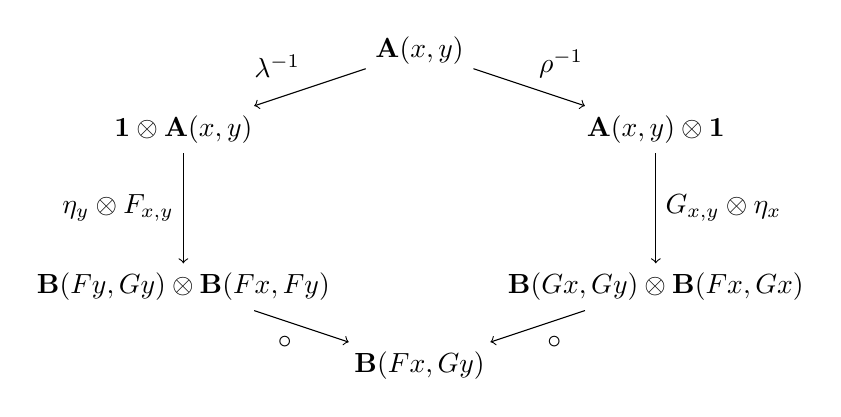
\begin{tikzpicture}
            \node (A) at (0, 0) {$\mathbf{A}(x,y)$};
            \node (IA) at (-3, -1) {$\mathbf{1}\otimes\mathbf{A}(x,y)$};
            \node (AI) at (3, -1) {$\mathbf{A}(x,y)\otimes\mathbf{1}$};
            \node (BF) at (-3, -3) {$\mathbf{B}(Fy,Gy)\otimes\mathbf{B}(Fx,Fy)$};
            \node (BG) at (3, -3) {$\mathbf{B}(Gx,Gy)\otimes\mathbf{B}(Fx,Gx)$};
            \node (B) at (0, -4) {$\mathbf{B}(Fx,Gy)$};
            \draw[->] (A) -- node[above left]{$\lambda^{-1}$} (IA);
            \draw[->] (A) -- node[above right]{$\rho^{-1}$} (AI);
            \draw[->] (IA) -- node[left]{$\eta_y\otimes F_{x,y}$} (BF);
            \draw[->] (AI) -- node[right]{$G_{x,y}\otimes\eta_x$} (BG);
            \draw[->] (BF) -- node[below left]{$\circ$} (B);
            \draw[->] (BG) -- node[below right]{$\circ$} (B);
        \end{tikzpicture}
        \caption{$\mathcal{V}$-naturality diagram.}
        \label{fig:v_naturality}
     \end{figure}

\subsection{Enriched constructions}

    \newdef{Functor tensor product}{\index{tensor product!functor}\label{cat:functor_tensor_product}
        Consider a covariant functor $\func{G}{C}{\mathcal{V}}$ and a contravariant functor $\cfunc{F}{C}{\mathcal{V}}$ into a monoidal category $\mathcal{V}$, where $\mathbf{C}$ does not have to be enriched over $\mathcal{V}$. The tensor product of $F$ and $G$ is defined as the following coend:
        \begin{gather}
            F\otimes_{\mathbf{C}}G := \int^{x\in\mathbf{C}}Fx\otimes Gx\,.
        \end{gather}
    }
    It should be noted that the above tensor product does not produce a new functor, instead it only gives an object in $\mathcal{V}$. A different type of tensor product, one that does give a functor, exists in the enriched setting (note that there is no relation between these two definitions).
    \newdef{Day convolution}{\index{Day convolution}
        Consider a monoidally cocomplete category $\mathcal{V}$, i.e.~cocomplete monoidal category for which the tensor product bifunctor is cocontinuous in each argument, together with a $\mathcal{V}$-enriched category $\mathbf{C}$. The convolution or tensor product (if it exists) of two $\mathcal{V}$-enriched functors $\func{F,G}{C}{\mathcal{V}}$ is defined as the following coend:
        \begin{gather}
            F\otimes_{\mathrm{Day}}G := \iint^{x,y\in\mathbf{C}}\mathbf{C}(x\otimes y,-)\otimes Fx\otimes Gy\,.
        \end{gather}
    }
    \begin{property}[Monoidal structure]
        In the case where $\mathbf{M}$ is a closed symmetric monoidal category, the Day convolution is associative and, hence, defines a monoidal structure on the functor category $[\mathbf{C},\mathbf{M}]$. The tensor unit is given by the functor (co)represented by the tensor unit in $\mathbf{C}$.
    \end{property}

    \newdef{Copower}{\index{co-!power}\index{power} % Both terms are indexed since copowers are rather important on their own.
        Consider a $\mathcal{V}$-enriched category $\mathbf{C}$. The copower (or tensor) functor $\func{\cdot}{\mathcal{V}\times C}{C}$ is defined by the following natural isomorphism:
        \begin{gather}
            \mathbf{C}(v\cdot x,y)\cong\mathcal{V}\big(v,\mathbf{C}(x,y)\big)\,.
        \end{gather}
        Dually, the power (or cotensor) functor $\func{[-,-]}{\mathcal{V}\times C}{C}$ is defined by the following natural isomorphism:
        \begin{gather}
            \mathbf{C}(x,[v,y])\cong\mathcal{V}\big(v,\mathbf{C}(x,y)\big)\,.
        \end{gather}
        If an enriched category admits all (co)powers, it is said to be \textbf{(co)powered} (over its enriching category).
    }
    \remark{\Cref{cat:internal_symmetry} says that every (closed) symmetric monoidal category $\mathbf{M}$ is powered over itself, the power just being the internal hom. The same holds for the copower, which is just the usual tensor product functor.}

    \begin{example}[Disjoint unions]
        Every (co)complete (locally) small category $\mathbf{C}$ admits the structure of a $\mathbf{Set}$-(co)powered category:
        \begin{gather}
            x^S := \prod_{s\in S}x\,,\\
            S\cdot x := \bigsqcup_{s\in S}x\,.
        \end{gather}
    \end{example}

    The definition and properties of internal hom-functors and (co)powers can be formalized as follows.
    \newdef{Two-variable adjunction}{\index{adjunction}\label{cat:two_variable_adjunction}
        Consider three categories $\mathbf{A,B}$ and $\mathbf{C}$. A two-variable adjunction $\mathbf{A}\times\mathbf{B}\rightarrow\mathbf{C}$ consists of three bifunctors:
        \begin{itemize}
            \item $\func{-\otimes-}{A\times B}{C}$,
            \item $\hom_L:\mathbf{A}^{op}\times\mathbf{C}\rightarrow\mathbf{B}$, and
            \item $\hom_R:\mathbf{B}^{op}\times\mathbf{C}\rightarrow\mathbf{A}$
        \end{itemize}
        admitting the following natural isomorphisms:
        \begin{gather}
            \mathbf{C}(x\otimes y,z)\cong\mathbf{A}\bigl(x,\hom_R(y,z)\bigr)\cong\mathbf{B}\bigl(y,\hom_L(x,z)\bigr)\,.
        \end{gather}
        It should be noted that fixing any of the variables gives rise to ordinary adjunctions in the sense of \cref{section:adjunction}.
    }
    \begin{property}[Powers and copowers]
        A category $\mathbf{C}$ enriched over a monoidal category $\mathcal{V}$ is powered and copowered over $\mathcal{V}$ exactly if the hom-functor $\mathbf{C}^{op}\times\mathbf{C}\rightarrow\mathcal{V}$ is the right adjoint in an enriched two-variable adjunction. The power and copower functors are then given by the other two adjoints.
    \end{property}

    The co-Yoneda lemma~\ref{cat:ninja_yoneda} can be generalized to the enriched setting:
    \begin{property}[Ninja Yoneda lemma]\index{Yoneda!reduction}\index{co-!Yoneda|see{Yoneda, reduction}}\label{cat:enriched_ninja_yoneda}
        Let $\cfunc{F}{C}{\mathcal{V}}$ be a contravariant functor (similar statements hold for covariant functors).
        \begin{align}
            &\int^{x\in\mathbf{C}}\mathbf{C}(-,x)\otimes Fx\cong F\\
            &\int_{x\in\mathbf{C}}\mathcal{V}\bigl(\mathbf{C}(x,-),Fx\bigr)\cong F\,.
        \end{align}
    \end{property}

    The following definition constructs Kan extensions in the enriched setting (these can be shown to reduce to \cref{cat:kan_extension} when enriching over $\mathbf{Set}$).
    \newadef{Kan extension}{\index{Kan!extension}\label{cat:enriched_kan_extension}
        Let $\mathbf{A,B}$ and $\mathbf{C}$ be categories enriched over a monoidal category $\mathcal{V}$. If $\mathbf{B}$ is assumed to be copowered over $\mathcal{V}$, left Kan extension of $\func{F}{A}{B}$ along $\func{G}{A}{C}$ can be defined through a coend:
        \begin{gather}
            \mathrm{Lan}_GF := \int^{x\in\mathbf{A}}\mathbf{C}(Gx,-)\cdot Fx\,.
        \end{gather}
        If $\mathbf{B}$ is assumed to be powered over $\mathcal{V}$, right Kan extension can be defined through an end:
        \begin{gather}
            \mathrm{Ran}_GF := \int_{x\in\mathbf{A}}\big[\mathbf{C}(-,Gx),Fx\big]\,.
        \end{gather}
        If $F$ is contravariant, the arguments of the hom-functors should simply be interchanged.
    }
    \remark{By choosing $\mathcal{V}=\mathbf{Set},\mathbf{C}=\mathbf{A}$ and $G=\mathbbm{1}_{\mathbf{A}}$ in the previous definition, one obtains the ninja Yoneda lemma~\ref{cat:ninja_yoneda}.}
    \begin{property}
        As already remarked in \cref{cat:preservation_kan_extension}, Kan extensions computed using (co)ends as above are strong.
    \end{property}

    \newadef{Functor tensor product}{\index{tensor product!functor}\label{cat:copower_product}
        Let $\mathbf{B}$ be a $\mathcal{V}$-enriched category. Consider a covariant functor $\func{G}{A}{B}$ and a contravariant functor $\cfunc{F}{A}{\mathcal{V}}$. The tensor product (\cref{cat:functor_tensor_product}) can be generalized whenever $\mathbf{B}$ is copowered over $\mathcal{V}$:
        \begin{gather}
            F\otimes_{\mathbf{A}}G := \int^{x\in\mathbf{A}}Fx\cdot Gx\,.
        \end{gather}
    }

\subsection{Weighted (co)limits}\index{limit!weighted}

    In this section the definition of ordinary limits and, in particular, the defining universal property~\ref{cat:limit_uproperty} is revisited. In this construction the constant functor $\Delta_x$ was one of the main ingredients. This functor can be factorized as $\mathbf{I}\rightarrow1\rightarrow\mathbf{C}$, where $1$ denotes the terminal category. On the level of morphisms this factorization takes the form $\mathbf{I}(i,j)\rightarrow\ast\rightarrow\mathbf{C}(x,x)$, where $\ast$ denotes the terminal one-element set. However, whenever the enriching context is not $\mathbf{Set}$, one does not necessarily have access to a terminal object.

    To avoid this issue, limits will first be redefined as representing objects. To this end, consider a general diagram $\func{D}{I}{C}$. By postcomposition with the Yoneda embedding one obtains the presheaf-valued diagram $\mathbf{C}(-,D-):\mathbf{I}\rightarrow[\mathbf{C}^{op}, \mathbf{Set}]$. Since presheaf categories are complete (\cref{cat:complete_presheaf_category}), the limit of this diagram exists: \[\mathbf{Set}\big(S,\lim\mathbf{C}(x,D-)\big)\cong\funccat{I}{Set}\bigl(\Delta_S,\mathbf{C}(x,D-)\bigr)\,.\] By restricting to the terminal set $S=\ast$, one obtains \[\lim\mathbf{C}(x,D-)\cong\funccat{I}{Set}\bigl(\Delta_\ast,\mathbf{C}(x,D-)\bigr)\,.\] If this presheaf is representable, one can use the continuity of the hom-functor, together with the fact that the Yoneda embedding is fully faithful, to show that the representing object is (isomorphic to) $\lim D$, i.e.
    \begin{gather}
        \funccat{I}{Set}(\Delta_\ast,\mathbf{C}(x,D-))\cong\mathbf{C}(x,\lim D)\,.
    \end{gather}

    ?? CLEAN THIS UP (note that continuity and pointwise definition was already mentioned for ordinary limits) ??

    \newdef{Weighted limit}{\index{limit!conical}\label{cat:weighted_limit}
        This definition can now be generalized by replacing the constant functor $\Delta_\ast$ by any functor $\func{W}{I}{Set}$. A representing object is then called the $W$-weighted limit of $D$. This object is often denoted by $\wlim{W}D$ or $\{W,D\}$. To distinguish weighted limits from ordinary ones, the latter are sometimes called \textbf{conical limits}.
    }

    \begin{remark}
        A motivation for this construction is the following. As was already pointed out in \cref{cat:global_elements_remark}, the mere knowledge of global elements $1\rightarrow x$ is often not enough to characterize an object $x$. In general one should look at the collection of generalized elements. When applying this ideology to the case of cones, one sees that replacing the functor $\Delta_\ast$ by a more general functor is the same as replacing the global elements $\ast\rightarrow Di$ by generalized elements $Wi\rightarrow Di$.
    \end{remark}

    The generalization to the enriched setting is now evident. There is no reference to the terminal object left, so one can replace $\mathbf{Set}$ by any enriching category. In the enriched setting, (co)end formulas for (weighted) limits will often be used.
    \newformula{Enriched weighted limits}{\label{cat:weighted_limits}
        By expressing the natural transformations as an end as in \cref{cat:natural_end} and by using the canonical powering in $\mathbf{Set}$, one can express ordinary weighted limits as follows:
        \begin{gather}
            \wlim{W}D\cong\int_{i\in\mathbf{I}}[Wi,Di]\,.
        \end{gather}
        The generalization to other enriching categories is now straightforward. Consider a diagram $\func{D}{I}{C}$ and a weight functor $\func{W}{I}{\mathcal{V}}$, where $\mathbf{C}$ is $\mathcal{V}$-enriched. If $\mathbf{C}$ is powered over $\mathcal{V}$, the $W$-weighted limit of $D$ is defined by the same formula as above:
        \begin{gather}
            \wlim{W}D:=\int_{i\in\mathbf{I}}[Wi,Di]\,.
        \end{gather}
        In a similar way one can define weighted colimits in copowered $\mathcal{V}$-categories as coends:
        \begin{gather}
            \colim^WD:=\int^{i\in\mathbf{I}}Wi\cdot Di\,.
        \end{gather}
        Here, the weight functor $W$ is required to be contravariant since colimits (and cocones in general) are natural transformations between contravariant functors.
    }
    \begin{property}[Weighted limits are Homs]
        In the case $\mathbf{C}=\mathcal{V}$, the powering functor becomes the internal hom and, therefore, one sees that weighted limits are given by (enriched) natural transformations (as was the case for ordinary conical limits).
    \end{property}

    In the following example the weighted colimit is calculated with respect to the Yoneda embedding:
    \begin{example}[Hom-functor]
        Consider a diagram $\func{D}{I}{C}$. When using the Yoneda embedding $\mathcal{Y}i = \mathbf{I}(-,i)$ as the weight functor, one obtains the following property by virtue of the Yoneda lemma:
        \begin{gather}
            \label{cat:weighted_hom_colimit}
            \colim^{\mathcal{Y}i}D\cong Di\,.
        \end{gather}
        A similar statement for weighted limits can be obtained with the covariant Yoneda embedding.
    \end{example}
    \newadef{Weighted (co)limits}{
        The above property can be used to axiomatize small weighted (co)limits in bicomplete categories:
        \begin{enumerate}
            \item\textbf{Yoneda}: For every object $i\in\ob{I}$ there exist isomorphisms
            \begin{gather}
                \wlim{\mathbf{I}(i,-)}D\cong Di\qquad\text{and}\qquad\colim^{\mathbf{I}(-,i)}D\cong Di\,.
            \end{gather}
            \item\textbf{Cocontinuity}: The weighted (co)limit functors are cocontinuous in the weights.
        \end{enumerate}
    }

    One can also express Kan extensions as weighted limits (this simply follows from expression \ref{cat:enriched_kan_extension}):
    \begin{property}[Kan extensions]\index{Kan!extension}
        Consider functors $\func{F}{A}{B}$ and $\func{G}{A}{C}$. If for every $x\in\ob{C}$ the weighted limit $\wlim{\mathbf{C}(x,G-)}F$ exists, these limits can be combined into a functor that can be shown to be the right Kan extension $\mathrm{Ran}_GF$. The left Kan extension can be obtained as a weighted colimit.
    \end{property}

    \begin{property}[Category of elements]\index{category!of elements}
        The weighted (co)limits of a functor (over $\mathbf{Set}$) can also be expressed in terms of the category of elements (\cref{cat:category_of_elements}) of the weight:
        \begin{gather}
            \wlim{W}F\cong\lim F\circ\mathbf{C}_W\,,
        \end{gather}
        where the limit on the right-hand side is a conical limit.

        The reason for the (co)end notation for categories of elements can also be explained by noting that these can actually be obtained as weighted (co)limits or (co)ends (here given for covariants functors):
        \begin{gather}
            \mathrm{El}(F) \cong \int^{c\in\mathbf{C}}Jc\times\mathrm{Disc}\,Fc\,,
        \end{gather}
        where $\cfunc{J}{C}{Cat}:c\mapsto c/\mathbf{C}$ assigns undercategories and $\func{\mathrm{Disc}}{Set}{Cat}$ sends sets to discrete categories.
    \end{property}

\section{Abelian categories}\label{section:abelian_categories}
\subsection{Additive categories}

    \newdef{Pre-additive category}{
        A (locally small) category enriched over $\mathbf{Ab}$, i.e.~a category in which every hom-set is an Abelian group and composition is bilinear.
    }

    \begin{property}\index{zero!object}
        Let $\mathbf{A}$ be a pre-additive category. The following statements are equivalent for an object $x\in\ob{A}$:
        \begin{itemize}
            \item $x$ is initial,
            \item $x$ is final, or
            \item $\mathbbm{1}_x = 0$.
        \end{itemize}
        It follows that every initial/terminal object in a pre-additive category is automatically a zero object (\cref{cat:zero_object}).
    \end{property}
    \begin{property}[Biproducts]\index{bi-!product}\index{direct!sum}
        In a pre-additive category the following isomorphism holds for all finitely indexed sets $\{x_i\}_{i\in I}$:
        \begin{gather}
            \prod_{i\in I}x_i\cong\bigsqcup_{i\in I}x_i\,.
        \end{gather}
        Finite (co)products in pre-additive categories are often called \textbf{direct sums}. In general, if a product and coproduct exist and are equal, one also speaks of a \textbf{biproduct}.
    \end{property}

    \newdef{Additive category}{\index{additive!category}
        A pre-additive category in which all finite products exist.
    }

    When working with additive categories, it is generally assumed that the associated functors are of a specific type:
    \newdef{Additive functor}{\index{additive!functor}\label{cat:additive_functor}
        Let $\mathbf{A},\mathbf{A'}$ be additive categories. A functor $\func{F}{A}{A'}$ is said to be additive if it preserves finite biproducts:
        \begin{enumerate}
            \item It preserves zero objects: $F\,0_{\mathbf{A}}\cong0_{\mathbf{A}'}$.
            \item There exists a natural isomorphism $F(x\oplus y)\cong Fx\oplus Fy$.
        \end{enumerate}
        This notion can be generalized to pre-additive categories. A functor between pre-additive categories is said to be additive if it acts as a group morphism on hom-spaces.
    }

    \newdef{Grothendieck group}{\index{Grothendieck!group}
        Let $\mathbf{A}$ be an additive category and consider its decategorification (\cref{cat:decategorification}). This set carries the structure of an Abelian monoid and, hence, the Grothendieck construction (\cref{group:grothendieck_completion}) can be applied to obtain an Abelian group $K(\mathbf{A})$. This group is called the Grothendieck group of $\mathbf{A}$.
    }

    In a (pre-)additive category one can some classical notions from (homological) algebra such as images and kernels.
    \newdef{Kernel}{\index{kernel}
        Let $f:x\rightarrow y$ be a morphism. A\footnote{`\textit{A}' since the kernel of a morphism is only determined up to an isomorphism.} kernel of $f$ is a morphism $k:z\rightarrow x$ such that:
        \begin{enumerate}
            \item $f\circ k = 0$.
            \item\textbf{Universal property}: Every morphism $k':z'\rightarrow x$ such that $f\circ k' = 0$ factors uniquely through $k$.
        \end{enumerate}
        This implies that a kernel of $f$ could equivalently be defined as the equalizer of $f$ and $0$.
    }
    \begin{notation}[Kernel]
        If the kernel of $f:x\rightarrow y$ exists, it is denoted by $\ker(f)$.
    \end{notation}

    \newdef{Cokernel}{
        Let $f:x\rightarrow y$ be a morphism. A cokernel of $f$ is a morphism $p:y\rightarrow z$ such that:
        \begin{enumerate}
            \item $p\circ f = 0$.
            \item\textbf{Universal property}: Every morphism $p':y\rightarrow z'$ such that $p'\circ f = 0$ factors uniquely through $p$.
        \end{enumerate}
        This implies that a cokernel of $f$ could equivalently be defined as the coequalizer of $f$ and 0.
    }
    \begin{notation}[Cokernel]
        If the cokernel of $f:x\rightarrow y$ exists, it is denoted by $\mathrm{coker}(f)$.
    \end{notation}
    \begin{remark}
        The name and notation of the kernel and the cokernel (in the categorical sense) is explained by remarking that $\ker(f)$ represents the functor
        \begin{gather}
            F:z\mapsto\ker\bigl(\mathbf{C}(z,x)\rightarrow\mathbf{C}(z,y)\bigr)\,,
        \end{gather}
        where $\ker$ denotes the algebraic kernel (\cref{group:kernel}), and similarly for he cokernel.
    \end{remark}

    \newdef{Pseudo-Abelian category}{\label{cat:pseudo_abelian}
        An additive category in which every projection/idempotent has a kernel.
    }
    \newdef{Pre-Abelian category}{
        An additive category in which every morphism has a kernel and cokernel.
    }
    \newdef{Abelian category}{\index{Abelian!category}
        A pre-Abelian category in which every mono is a kernel and every epi is a cokernel or, equivalently, if for every morphism $f$ there exists an isomorphism
        \begin{gather}
            \coker\!\bigl(\!\ker(f)\bigr)\cong\ker\!\bigl(\!\coker(f)\bigr)\,.
        \end{gather}
    }

    \begin{property}[Injectivity and surjectivity]
        In Abelian categories, a morphism is monic if and only if it is injective, i.e.~its kernel is 0. Analogously, a morphism is epic if and only if it is surjective, i.e.~its cokernel is 0.
    \end{property}

    \newdef{Linear category}{\index{category!linear}
        Let $\mathbf{Vect}_K$ denote the category of vector spaces over the base field $K$. A $K$-linear category is a category enriched over $\mathbf{Vect}_K$. (If the base field is clear, the subscript is often left implicit.)
    }

\subsection{Exact functors}

    \newdef{Exact functor}{\index{exact!functor}
        Let $\func{F}{A}{A'}$ be an additive functor between additive categories.
        \begin{itemize}
            \item $F$ is said to be left-exact if it preserves kernels.
            \item $F$ is said to be right-exact if it preserves cokernels.
            \item $F$ is said to be exact if it is both left- and right-exact.
        \end{itemize}
    }
    \begin{result}
        The previous definition implies the following properties (which can in fact be used as an alternative definition):
        \begin{itemize}
            \item If $F$ is left-exact, it maps an exact sequence of the form \[0\longrightarrow x\longrightarrow y\longrightarrow z\]
            to an exact sequence of the form \[0\longrightarrow Fx\longrightarrow Fy\longrightarrow Fz\,.\]
            \item If $F$ is right-exact, it maps an exact sequence of the form \[x\longrightarrow y\longrightarrow z\longrightarrow 0\]
            to an exact sequence of the form \[Fx\longrightarrow Fy\longrightarrow Fz\longrightarrow 0\,.\]
            \item If $F$ is exact, it maps short exact sequences to short exact sequences.
        \end{itemize}
    \end{result}

    \begin{notation}[Left or right]
        The category of left modules ${}_R\mathbf{Mod}$ over a ring $R$ is equivalent (as an Abelian category) to the category of right modules $\mathbf{Mod}_{R^{op}}$ over the opposite ring $R$. For this reason one often makes no difference between left and right modules (only bimodules are truly relevant) and ``the category of $R$-modules'' is just denoted by $R\mathbf{Mod}$.
    \end{notation}

    \begin{theorem}[Freyd--Mitchell embedding theorem]\index{Freyd--Mitchell}\index{embedding!theorem|see{Freyd--Mitchell}}\label{cat:freyd_mitchell}
        Every small Abelian category admits a fully faithful, exact functor into a category of the form $R\mathbf{Mod}$ for some unital ring $R$.
    \end{theorem}

    \begin{theorem}[Eilenberg-Watts]\index{Eilenberg-Watts}
        Let $R,S$ be two (not necessarily unital) rings. The tensor product functor induces an equivalence between the category of $R\text{-}S$-bimodules and the category of cocontinuous functors $R\mathbf{Mod}\rightarrow S\mathbf{Mod}$.
    \end{theorem}

\subsection{Finiteness}

    \newdef{Simple object}{\index{simple!object}
        Let $\mathbf{A}$ be an Abelian category. An object $a\in\ob{A}$ is said to be simple if the only subobjects of $a$ are $0$ and $a$ itself. An object is said to be semisimple if it is a direct sum of simple obejcts.
    }
    \newdef{Semisimple category}{
        A category is said to be semisimple if every object is semisimple (where in general the direct sums are taken over finite index sets).
    }

    \newdef{Jordan--H\"older series}{\index{finite}\index{Jordan--H\"older!series}
        A filtration \[0\longrightarrow x_1\longrightarrow x_2\longrightarrow\cdots\longrightarrow x_n=x\] of an object $x$ is said to be a Jordan--H\"older series if the quotient objects $x_i/x_{i-1}$ are simple for all $i\leq n$. If the series has finite length, the object $x$ is said to be \textbf{finite}.
    }
    \begin{theorem}[Jordan--H\"older]\index{Jordan--H\"older}
        If an object in an Abelian category is finite, all of its Jordan--H\"older series have the same length. In particular, the multiplicities of simple objects are the same for all such series.
    \end{theorem}

    \begin{theorem}[Krull--Schmidt]\index{Krull--Schmidt}\index{indecomposable}
        Any object in an Abelian category of finite length admits a unique decomposition as a direct sum of indecomposable objects\footnote{An object is \textbf{indecomposable} if it cannot be written as a direct sum of its subobjects.}.
    \end{theorem}

    \newdef{Locally finite}{\label{cat:locally_finite}
        A $k$-linear Abelian category is said to be locally finite if it satisfies the following conditions:
        \begin{enumerate}
            \item every hom-space is finite-dimensional, and
            \item every object has finite length.
        \end{enumerate}
    }
    \newdef{Finite}{\index{finite}
        A $k$-linear Abelian category is said to be finite if it satisfies the following conditions:
        \begin{enumerate}
            \item It is locally finite.
            \item It has enough projectives or, equivalently, every simple object has a \textit{projective cover}.
            \item The set of isomorphism classes of simple objects is finite.
        \end{enumerate}
    }

    \begin{theorem}[Schur's lemma]\index{Schur!lemma}\label{cat:schur_lemma}
        Let $\mathbf{A}$ be an Abelian category. For every two simple objects $x,y$, all nonzero morphisms $x\rightarrow y$ are isomorphisms. In particular, if $x,y$ are two non-isomorphic simple objects, then $\mathbf{A}(x,y)=0$. Furthermore, $\mathbf{A}(x,x)$ is a division ring for every simple object $x$.
    \end{theorem}
    \begin{result}
        If $\mathbf{A}$ is locally finite and $k$ is algebraically closed, then $\mathbf{A}(x,x)\cong k$ for all simple objects $x$. This follows from the fact that the only finite-dimensional division algebra over an algebraically closed field is the field itself.
    \end{result}

    The Freyd--Mitchell theorem~\ref{cat:freyd_mitchell} can be adapted to the finite linear case as follows.
    \begin{theorem}[Deligne]\index{Deligne}
        Every finite $k$-linear Abelian category is $k$-linearly equivalent to a category of the form $A\mathbf{Mod}^{\mathrm{fin}}$ for $A$ a finite-dimensional $k$-algebra.
    \end{theorem}

    \begin{construct}[Deligne tensor product]\index{Deligne|seealso{tensor product}}\index{tensor product!Deligne}
        Let $\mathbf{A},\mathbf{B}$ be two Abelian categories. Their Deligne (tensor) product is defined (if it exists) as the category $\mathbf{A}\boxtimes\mathbf{B}$ for which there exists a bijection between right exact functors $\mathbf{A}\boxtimes\mathbf{B}\rightarrow\mathbf{C}$ and right exact functors $\mathbf{A}\times\mathbf{B}\rightarrow\mathbf{C}$ (the latter being right exact in each argument).

        For finite Abelian categories it can be shown that their Deligne product always exists. By the Deligne embedding theorem one can find an explicit description. Consider two finite-dimensional $k$-algebras $A, B$. The category $A\mathbf{Mod}^{\mathrm{fin}}\boxtimes B\mathbf{Mod}^{\mathrm{fin}}$ is equivalent to the category $A\otimes_kB\mathbf{Mod}^{\mathrm{fin}}$.
    \end{construct}

\section{Monoidal categories II: Duality}\label{section:duality}

    The general theory of monoidal categories was introduced in \cref{section:monoidal_categories}.

    \newdef{Dual object}{\index{dual!object}\label{hda:dual}
        Let $(\mathbf{C},\otimes,\mathbf{1})$ be a monoidal category and consider an object $x\in\ob{C}$. A left dual\footnote{$x$ is called the \textbf{right dual} of $x^*$. The right dual of $y$ is often denoted by ${}^*y$.} of $x$ is an object in $x^*\in\ob{C}$ together with two morphisms $\eta:\mathbf{1}\rightarrow x\otimes x^*$ and $\varepsilon:x^*\otimes x\rightarrow\mathbf{1}$, called the \textbf{unit} and \textbf{counit} morphisms\footnote{Also called the \textbf{coevaluation} and \textbf{evaluation} morphisms.}, such that the diagrams in \cref{fig:dual_objects} commute. $x$ is said to be \textbf{dualizable} if it admits a left dual.
    }

    \begin{figure}[ht!]
        \centering
        \begin{subfigure}[b]{0.49\textwidth}
            \centering
            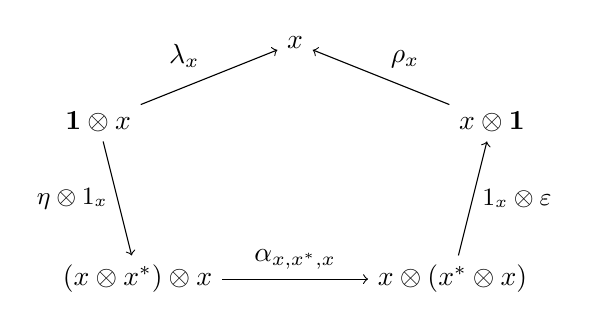
\begin{tikzpicture}
                \node (X) at (0, 0) {$x$};
                \node (1X) at (-2.5, -1) {$\mathbf{1}\otimes x$};
                \node (X1) at (2.5, -1) {$x\otimes\mathbf{1}$};
                \node (1XXX) at (-2, -3) {$(x\otimes x^*)\otimes x$};
                \node (XXX1) at (2, -3) {$x\otimes(x^*\otimes x)$};
                \draw[->] (1X) -- node[above left]{$\lambda_x$} (X);
                \draw[->] (X1) -- node[above right]{$\rho_x$} (X);
                \draw[->] (1X) -- node[left]{\small $\eta\otimes\mathbbm{1}_x$} (1XXX);
                \draw[->] (XXX1) -- node[right]{\small $\mathbbm{1}_x\otimes\varepsilon$} (X1);
                \draw[->] (1XXX) -- node[above]{$\alpha_{x,x^*,x}$} (XXX1);
            \end{tikzpicture}
            \caption{Dual object I.}
            \label{fig:dual_object1}
        \end{subfigure}
        \begin{subfigure}[b]{0.49\textwidth}
            \centering
            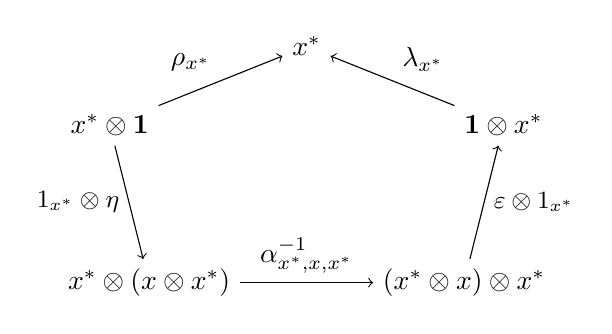
\begin{tikzpicture}
                \node (X) at (0, 0) {$x^*$};
                \node (X1) at (-2.5, -1) {$x^*\otimes\mathbf{1}$};
                \node (1X) at (2.5, -1) {$\mathbf{1}\otimes x^*$};
                \node (XXX1) at (-2, -3) {$x^*\otimes(x\otimes x^*)$};
                \node (1XXX) at (2, -3) {$(x^*\otimes x)\otimes x^*$};
                \draw[->] (X1) -- node[above left]{$\rho_{x^*}$} (X);
                \draw[->] (1X) -- node[above right]{$\lambda_{x^*}$} (X);
                \draw[->] (X1) -- node[left]{\small $\mathbbm{1}_{x^*}\otimes\eta$} (XXX1);
                \draw[->] (1XXX) -- node[right]{\small $\varepsilon\otimes\mathbbm{1}_{x^*}$} (1X);
                \draw[->] (XXX1) -- node[above]{$\alpha^{-1}_{x^*,x,x^*}$} (1XXX);
            \end{tikzpicture}
            \caption{Dual object II.}
            \label{fig:dual_object2}
        \end{subfigure}
        \caption{Dualizable objects.}
        \label{fig:dual_objects}
    \end{figure}

    \newdef{Rigid category}{\index{category!rigid}\index{category!autonomous}
        A monoidal category that has all duals. These categories are also said to be \textbf{autonomous}. If only left (resp.~right) duals exist, the category is said to be left (resp.~right) rigid.
    }

    \begin{property}[Braided categories]\label{hda:braided_rigid}
        In general it is not true that left and right duals coincide. However, in a braided monoidal category this is the case.
    \end{property}
    \newdef{Compact closed category}{\index{category!compact closed}
        A symmetric rigid category.
    }

    \begin{example}[FinVect]\index{dual!space}\index{resolution!of the identity}
        Consider the category $\mathbf{FinVect}$ of finite-dimensional vector spaces (the ground field is assumed to be $\mathbb{R}$). The categorical dual of a vector space $V$ is the algebraic dual $V^*$. The unit morphism is given by the `resolution of the identity':
        \begin{gather}
            \eta:\mathbf{1}\rightarrow V\otimes V^*:1\mapsto\sum_{i=1}^{\dim(V)}e_i\otimes\phi^i\,,
        \end{gather}
        where $\{e_i\}$ and $\{\phi^i\}$ are bases of $V$ and $V^*$, respectively.

        It should be noted that the category $\mathbf{Vect}$ of all vector spaces is not rigid. By \cref{hda:braided_rigid} above, left and right duals coincide in any braided monoidal category (such as $\mathbf{Vect}$), but for infinite-dimensional vector spaces it is known that $A\cong(A^*)^*$ never holds and as such rigidity cannot be extended to $\mathbf{Vect}$.
    \end{example}

    \begin{property}[Tannaka duality]\index{Tannaka duality}
        Consider the category $\mathcal{V}=\mathbf{FinVect}_K$. Using coends one can reconstruct the base field from its modules, i.e.~the objects in $\mathcal{V}$:
        \begin{gather}
            \int^{V\in\mathcal{V}}V^*\otimes V\cong K\,.
        \end{gather}
        This result can be shown to hold for all compact closed categories $\mathcal{V}$. In this context it is known as \textbf{Tannaka reconstruction}. A more general statement goes as follows:
        \begin{gather}
            \int^{V\in\mathcal{V}}\mathcal{V}(V,-)\otimes V\cong\mathrm{id}_{\mathcal{V}}\,.
        \end{gather}
        For $\mathcal{V}=\mathbf{FinVect}_K$, the components $\eta_V:\mathcal{V}(V,V)\rightarrow K$ of the coend can be shown to coincide with the trace and as such the trace obtains a universal property.
    \end{property}
    \begin{remark}
        This property can also be generalized by replacing $\mathcal{V}$ by a category of modules $A\mathbf{Mod}$ for some finite-dimensional algebra $A$. The end and coend give the algebra $A$ and its dual $A^*$, respectively.
    \end{remark}

    \newdef{Symmetric monoidal dagger category}{\index{category!dagger}
        A symmetric monoidal category $(\mathbf{C},\otimes,\mathbf{1})$ that also carries the structure of a dagger category (\cref{cat:dagger_category}) such that
        \begin{gather}
            (f\otimes g)^\dag = f^\dag\otimes g^\dag
        \end{gather}
        and such that the coherence and braiding morphisms are unitary.
    }
    \newdef{Dagger-compact category}{
        A symmetric monoidal dagger category that is also a compact closed category such that the following diagram commutes for all objects:
        \begin{gather*}
            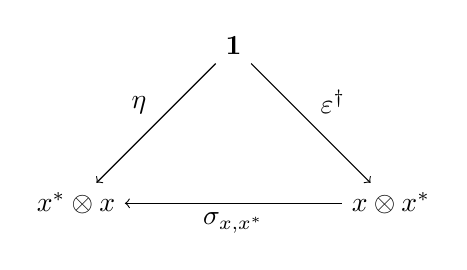
\begin{tikzpicture}
                \node (1) at (0, 0) {$\mathbf{1}$};
                \node (X*X) at (-2, -2) {$x^*\otimes x$};
                \node (XX*) at (2, -2) {$x\otimes x^*$};
                \draw[->] (1) -- node[above left]{$\eta$} (X*X);
                \draw[->] (1) -- node[above right]{$\varepsilon^\dagger$} (XX*);
                \draw[<-] (X*X) -- node[below]{$\sigma_{x,x^*}$} (XX*);
            \end{tikzpicture}
        \end{gather*}
    }

    The trace on $\mathbf{FinVect}$ can be generalized as follows:
    \newdef{Trace}{\index{trace!categorical}
        Let $(\mathbf{C},\otimes,\mathbf{1})$ be a rigid category and let $f\in\mathbf{C}(x,x^{**})$. The left (\textbf{categorical} or \textbf{quantum}) trace of $f$ is defined as the following morphism in $\End_{\mathbf{C}}(\mathbf{1})$:
        \begin{gather}
            \tr^L(f):=\varepsilon_{x^*}\circ(f\otimes\mathbbm{1}_{x^*})\circ\eta_x\,.
        \end{gather}
        For $f\in\mathbf{C}(x,{}^{**}x)$, the right trace is defined similarly:
        \begin{gather}
            \tr^R(f):=\varepsilon_{{}^{**}x}\circ(\mathbbm{1}_x\otimes f)\circ\eta_{{}^*x}\,.
        \end{gather}
    }
    \begin{property}
        The following linear algebra-like properties hold for the categorical trace:
        \begin{itemize}
            \item $\tr^L(f) = \tr^R(f^*)$,
            \item $\tr^L(f\otimes g) = \tr^L(f)\tr^L(g)$, and
            \item for additive categories: $\tr^L(f\oplus g) = \tr^L(f) + \tr^L(g)$.
        \end{itemize}
        The second and third property can be stated analogously for the right trace.
    \end{property}

    \newdef{Pivotal category}{\index{pivotal structure}
        Let $\mathbf{C}$ be a rigid monoidal category. A pivotal structure on $\mathbf{C}$ is a monoidal natural isomorphism $\psi:\mathrm{id}_{\mathbf{C}}\Rightarrow\ast\ast$.
    }

    \newdef{Dimension}{\index{dimension!pivotal}\label{hda:pivotal_dimension}
        Let $(\mathbf{C},\psi)$ be a pivotal category and consider an object $x\in\ob{C}$. The dimension of $x$ is defined as follows:
        \begin{gather}
            \dim_\psi(x) := \tr^L(\psi_x)\,.
        \end{gather}
    }

    \newdef{Spherical category}{\index{spherical structure}
        A pivotal category $(\mathbf{C},\psi)$ in which the left and right traces with respect to $\psi$ coincide: $\dim_\psi(x)=\dim_\psi(x^*)$ for all $x\in\ob{C}$.
    }

    \newdef{Calabi--Yau category}{\index{Calabi--Yau!category}\label{hda:calabi_yau}
        A $\mathbf{Vect}$-enriched category $\mathbf{C}$ equipped with a \textbf{trace} functional
        \begin{gather}
            \tr_x:C(x,x)\rightarrow K
        \end{gather}
        for each object $x\in\ob{C}$ such that the induced pairing
        \begin{gather}
            \langle\cdot,\cdot\rangle:C(x,y)\otimes C(y,x)\rightarrow K:f\otimes g\mapsto\tr_x(g\circ f)
        \end{gather}
        is symmetric and nondegenerate.
    }
    \begin{example}
        A one-object Calabi--Yau category is the (pointed) monoid delooping of a Frobenius algebra (\cref{linalgebra:frobenius}).
    \end{example}

\section{Tensor and fusion categories}

    Some definitions might slightly differ from the ones in the main references and some properties might be stated less generally. $K$ denotes an algebraically closed field (this will often be $\mathbb{C}$).

    \newdef{Tensor category}{\index{tensor!category}
        A monoidal category with the following properties:
        \begin{enumerate}
            \item it is rigid,
            \item it is Abelian,
            \item it is $K$-linear in a way compatible with the Abelian structure,
            \item $\End(\mathbf{1})\cong K$, and
            \item $-\otimes-$ is bilinear on morphisms.
        \end{enumerate}
        Some authors (such as~\citet{etingof_tensor_2016}) also add `locally finite' as a condition (\cref{cat:locally_finite}).
    }
    \remark{If $K$ is not algebraically closed, one should replace the fourth condition by the condition that $\mathbf{1}$ is a simple object. However, if $K$ is algebraically closed, these statements are equivalent.}

    \newdef{Pointed tensor category}{\index{pointed!tensor category}
        A tensor category where all of the simple objects are (weakly) invertible.
    }

    \newdef{Fusion category}{\index{fusion!category}
        A semisimple finite tensor category.
    }

    \begin{property}
        Let $\mathbf{C}$ be a fusion category. There exists a natural isomorphism $\mathbbm{1}_{\mathbf{C}}\cong\ast\ast$.
    \end{property}
    \begin{remark}
        Although any fusion category admits a natural isomorphism between an object and its double dual, this morphism does not need to be monoidal. The fact that all fusion categories are pivotal was conjectured by \textit{Etingof, Ostrik} and \textit{Nikshych}. Currently the best one can do for a general fusion category is a monoidal natural transformation between the identity functor and the fourth dualization functor $\mathbbm{1}_{\mathbf{C}}\cong\ast\ast\ast\,\ast$.
    \end{remark}

    \newdef{Categorical dimension}{\index{dimension!categorical}
        Consider a fusion category $\mathbf{C}$ and choose a natural isomorphism $\psi:\mathbbm{1}_{\mathbf{C}}\cong\ast\ast$. For every simple object $x\in\ob{C}$ one can define a dimension function, sometimes called the \textbf{norm squared}, in the following way:
        \begin{gather}
            |x|^2 := \tr(\psi_x)\tr\bigl((\psi_x^{-1})^*\bigr)\,.
        \end{gather}
        If $\mathbf{C}$ is pivotal, this becomes $|x|^2 = \dim_\psi(x)\dim_\psi(x^*)$. In particular, when $\mathbf{C}$ is spherical, this becomes $|x|^2 = \dim_\psi(x)^2$.

        The categorical dimension, sometimes called the \textbf{M\"uger dimension}, is then defined as follows:
        \begin{gather}
            \dim(\mathbf{C}) := \sum_{x\in\mathcal{O}(\mathbf{C})}|x|^2\,,
        \end{gather}
        where $\mathcal{O}(\mathbf{C})$ denotes the set of isomorphism classes of simple objects.
    }
    \remark{It should be noted that the above quantities do not depend on the choice of isomorphism $\psi_x:x\cong x^{**}$ since all of them only differ by a scale factor.}
    \begin{property}[Nonzero dimension]
        For any fusion category $\mathbf{C}$ one has that $\dim(\mathbf{C})\neq 0$. In particular, if $K=\mathbb{C}$, then $\dim(\mathbf{C})\geq1$ (since the norm squared of any simple object is then also positive).
    \end{property}

    \newdef{$G$-graded fusion category}{\index{G-!grading}
        A semisimple linear category $\mathbf{C}$ is said to have a \textbf{$G$-grading}, where $G$ is a finite group, if it can be decomposed as follows:
        \begin{gather}
            \mathbf{C}\cong\bigoplus_{g\in G}\mathbf{C}_g\,,
        \end{gather}
        where every $\mathbf{C}_g$ is linear and semisimple. A fusion category $\mathbf{C}$ is said to be a ($G$-)graded fusion category if it admits a $G$-grading such that $\mathbf{C}_g\otimes\mathbf{C}_h\subseteq\mathbf{C}_{gh}$ for all $g,h\in G$.
    }

    \begin{example}[$G$-graded vector spaces]\label{hda:g_graded}
        Define the category $\mathbf{Vect}_G^\omega$ as having the same objects and morphisms as $\mathbf{Vect}_G$, the category of $G$-graded vector spaces, but with the associator given by the the 3-cocycle $\omega\in H^3(G;K^\times)$.
    \end{example}
    \begin{property}
        Any pointed fusion category is equivalent to a category of the form $\mathbf{Vect}_G^\omega$ for some $G$ and $\omega\in H^3(G;K^\times)$.
    \end{property}

    \begin{theorem}[Tannaka duality]\index{Tannaka duality}
        The category of modules of a weak Hopf algebra has the structure of a fusion category. Conversely, any fusion category can be obtained as the category of modules of a weak Hopf algebra.
    \end{theorem}

\section{Ribbon and modular categories}

    \newdef{Ribbon structure}{
        Consider a braided monoidal category $(\mathbf{C},\otimes,\mathbf{1})$ with braiding $\sigma$. A \textbf{twist} or \textbf{balancing} is a natural endomorphism $\theta$ such that the following equation is satisfied for all $x,y\in\ob{C}$:
        \begin{gather}
            \theta_{x\otimes y} = (\theta_x\otimes\theta_y)\circ\sigma_{y,x}\circ\sigma_{x,y}\,.
        \end{gather}
        If in addition $\mathbf{C}$ is rigid and the twist satisfies $\theta_{x^*} = (\theta_x)^*$ for all $x\in\ob{C}$, one speaks of a ribbon or \textbf{tortile} category.
    }

    \newdef{Drinfel'd morphism}{\index{Drinfel'd!morphism}
        Let $(\mathbf{C},\otimes,\mathbf{1})$ be a rigid braided monoidal category with braiding $\sigma$. This structure admits a canonical natural automorphism $\mathrm{id}_{\mathbf{C}}\cong\ast\ast$ defined as follows:
        \begin{gather}
            x\xrightarrow{\mathbbm{1}_x\otimes\eta_{x^*}}x\otimes x^*\otimes x^{**}\xrightarrow{\sigma_{x,x^*}\otimes\mathbbm{1}_{x^{**}}}x^*\otimes x\otimes x^{**}\xrightarrow{\varepsilon_x\otimes\mathbbm{1}_{x^{**}}}x^{**}\,.
        \end{gather}
    }
    \begin{property}
        Let $\mathbf{C}$ be a braided monoidal category. Consider the canonical natural isomorphism $u:\mathrm{id}_{\mathbf{C}}\cong\ast\ast$ defined above. Any natural isomorphism $\psi:\mathrm{id}_{\mathbf{C}}\cong\ast\ast$ can be written as $u\circ\theta$ where $\theta\in\Aut(\mathbbm{1}_{\mathbf{C}})$. It is not hard to see that this natural isomorphism is monoidal (and, hence, pivotal) exactly when $\theta$ is a twist. If $\mathbf{C}$ is a fusion category then the pivotal structure is spherical if and only if $\theta$ determines a ribbon structure.
    \end{property}

    \newdef{Premodular category}{
        A ribbon fusion category. Equivalently, a spherical braided fusion category.
    }
    \newdef{$S$-matrix}{\index{S-matrix}
        Given a premodular category $\mathbf{M}$ with braiding $\sigma$, the $S$-matrix is defined as follows:
        \begin{gather}
            S_{xy} := \tr(\sigma_{y,x}\circ\sigma_{x,y})\,,
        \end{gather}
        where $x,y\in\mathcal{O}(\mathbf{M})$ are (isomorphism classes of) simple objects. Since in a premodular category there are only finitely many isomorphism classes of simple objects (denote this number by $\mathcal{I}$), one can see that $S$ is a $\mathcal{I}\times\mathcal{I}$-matrix.
    }

    \newdef{Modular category\footnotemark}{\index{modular!category}\label{hda:modular_category}
        \footnotetext{`Modular tensor category' is often abbreviated as \textbf{MTC}.}
        \nomenclature[A_MTC]{MTC}{modular tensor category}
        A premodular category for which the $S$-matrix is invertible.
    }

    \begin{property}
        Let $\mathbf{M}$ be a modular category with $S$-matrix $S$ and define the following matrix:
        \begin{gather}
            E_{xy} :=
            \begin{cases}
                1&x=y^*\\
                0&\text{otherwise}.
            \end{cases}
        \end{gather}
        The following relation with the categorical dimension of $\mathbf{M}$ is obtained:
        \begin{gather}
            S^2 = \dim(\mathbf{M})E\,.
        \end{gather}
    \end{property}

    \begin{formula}[Verlinde]
        Consider a modular category $\mathbf{M}$ with $S$-matrix $S$. Let $\mathcal{O}(\mathbf{M})$ denote the set of isomorphism classes of simple objects and let $\dim$ denote the dimension associated to the spherical structure on $\mathbf{M}$. Using the formula
        \begin{gather}
            S_{xy}S_{xz} = \dim(x)\sum_{w\in\mathcal{O}(\mathbf{M})}N^w_{yz}S_{xw}
        \end{gather}
        for all $x,y,z\in\mathcal{O}(\mathbf{M})$, one obtains the following important relation:
        \begin{gather}
            \sum_{w\in\mathcal{O}(\mathbf{M})}\frac{S_{wy}S_{wz}S_{wx^*}}{\dim(w)} = \dim(\mathbf{M})N^x_{yz}\,.
        \end{gather}
        This property implies that the $S$-matrix of a modular category determines the fusion coefficients of the underlying fusion category.
    \end{formula}

\section{Module categories}

    By categorifying the definition of a module over a ring (\cref{algebra:module}), one obtains the notion of a module category.
    \newdef{Module category}{\index{module!category}
        Let $\mathbf{M}$ be a monoidal category. A left $\mathbf{M}$-module (category) is a category $\mathbf{C}$ equipped with a bilinear functor $\func{\triangleright}{M\times C}{C}$  together with natural isomorphisms that categorify the associativity and unit conditions of modules (these are also required to be compatible with the associator and unitors of $\mathbf{M}$).
    }
    \remark{Similar to how a $G$-set can be defined as a functor $\mathbf{B}G\rightarrow\mathbf{Set}$ (\cref{cat:delooping_representation}), one can define a module category as a 2-functor $\mathbf{BM}\rightarrow\mathbf{Cat}$.}

    Analogous to \cref{cat:internal_hom} one can also define internal homs for module categories.
    \newdef{Internal hom}{\index{internal!hom}
        Consider a left $\mathbf{M}$-module $\mathbf{C}$. Given two objects $x,y\in\ob{C}$ one defines their internal hom (if it exists) as the object $\underline{\hom}(x,y)\in\ob{M}$ satisfying the following condition
        \begin{gather}
            \mathbf{C}(m\triangleright x,y)\cong\mathbf{M}\bigl(m,\underline{\hom}(x,y)\bigr)
        \end{gather}
        for all $m\in\ob{M}$.
    }
    \begin{property}
        It should be noted that for the case $\mathbf{C}\equiv\mathbf{M}$, where the action is given by the tensor product in $\mathbf{M}$, one obtains \cref{cat:internal_hom} as a particular case.
    \end{property}

\section{Higher vector spaces}\index{2-!vector space}
\subsection{Kapranov--Voevodksy 2-vector spaces}

    The guiding principle for the definition of 2-vector spaces in this section will be the generalization of certain observations from studying the category $\mathbf{Vect}$ of ordinary vector spaces. Linear maps between vector spaces can (at least in finite dimensions) be represented as matrices with coefficients in the ground field $K$. Coincidentally this ground field is also the tensor unit in $\mathbf{Vect}$. At the same time, all finite-dimensional vector spaces are isomorphic to spaces of the form $K^n$, where $n$ is given by the dimension of the vector space.

    \newdef{2-vector space}{\index{Kapranov--Voevodsky 2-vector space}
        To define 2-vector spaces, \textit{Kapranov} and \textit{Voevodsky} lifted these observations to categories by replacing the ground field $K$ by the category $\mathbf{Vect}_K$. To wit, $\mathbf{2Vect}_K$ is defined as the 2-category consisting of the following data:
        \begin{itemize}
            \item\textbf{Objects}: Finite products of the form $\mathbf{Vect}_K^n$.
            \item\textbf{1-morphisms}: Collections $\|A_{ij}\|$ of finite-dimensional $K$-vector spaces, called \textbf{2-matrices}.
            \item\textbf{2-morphisms}: Collections $(f_{ij})$ of linear maps between finite-dimensional $K$-vector spaces.
        \end{itemize}
        The multiplication (or composition) of 1-morphisms is defined in analogy to the multiplication of ordinary matrices, but where the usual sum and product are replaced by the direct sum and tensor product.
    }

    A seemingly more formal definition uses the concepts of \textit{ring} and module categories.
    \begin{adefinition}
        A 2-vector space is a lax module category over $\mathbf{Vect}$ that is module-equivalent to $\mathbf{Vect}^n$ for some $n\in\mathbb{N}$. The 2-category $\mathbf{2Vect}$ is then defined as the 2-category with objects these 2-vector spaces, as 1-morphisms the associated $\mathbf{Vect}$-module functors and as 2-morphisms the module natural transformations.
    \end{adefinition}

\subsection{Baez--Crans 2-vector spaces}\label{section:baez_crans}

    \newdef{2-vector space}{\index{Baez--Crans 2-vector space}\index{linear!functor}
        A category internal to $\mathbf{Vect}$. The morphism are \textbf{linear functor}, i.e.~functors internal to $\mathbf{Vect}$.
    }
    \remark{The above definition should not be confused with that of categories and functors enriched over $\mathbf{Vect}$.}

    \begin{example}[Ground field]
        The ground field $K$ can be categorified to a 2-vector spaces by taking $K_0=K_1:=K$ and $s=t=e:=\mathbbm{1}_K$. This object serves as a unit for the tensor product on $\mathbf{2Vect}_K$.
    \end{example}

    \begin{property}[Chain complexes]
        There exists an equivalence between the (2-)categories of 2-vector spaces and 2-term chain complexes.
        \begin{mdframed}[roundcorner=10pt, linecolor=blue, linewidth=1pt]
            \begin{proof}[Sketch of construction]
                Given a 2-vector space $(V_0,V_1)$, one can build a chain complex $C_\bullet$ as follows:
                \begin{itemize}
                    \item $C_0 := V_0$,
                    \item $C_1 := \ker(s)$, and
                    \item $d := t|_{C_1}$,
                \end{itemize}
                where $s,t$ are the source and target morphisms.
            \end{proof}
        \end{mdframed}
    \end{property}
    \remark{The equivalence (on the level of ordinary categories) is an instance of the Dold--Kan correspondence (\cref{model:dold_kan}).}

    \newdef{Arrow part}{\index{arrow}
        Consider a 2-vector space $V=(V_0,V_1)$. For any morphism $f\in V_1$ one defines the arrow part as follows:
        \begin{gather}
            \vec{f} := f - e\bigl(s(f)\bigr)\,,
        \end{gather}
        where $e,s$ are the identity and source morphisms in $V$. Any map can thus be recovered from its arrow part and its source. This allows to identify a map $f\in V_1$ with the pair $\big(s(f),\vec{f}\,\big)$. Using arrow parts one can rewrite the composition law of morphisms in an intuitive way:
        \begin{gather}
            g\circ f = \bigl(s(f),\vec{f} + \vec{g}\,\bigr)\,.
        \end{gather}
    }

    \newdef{Antisymmetric morphism}{\index{antisymmetry}
        A natural morphism between $n$-linear functors in $\mathbf{2Vect}$ is said to be \textbf{completely antisymmetric} if its arrow part is completely antisymmetric.
    }

\section{Higher Lie theory}
\subsection{Lie superalgebras}

    \newdef{Internal Lie algebra}{\index{Lie!algebra}
        Let $(\mathbf{C},\otimes,\mathbf{1})$ be a linear symmetric monoidal category with braiding $\sigma$. A Lie algebra internal to $\mathbf{C}$ is an object $L\in\ob{C}$ and a morphism \[[\cdot,\cdot]:L\otimes L\rightarrow L\] satisyfing the following conditions:
        \begin{enumerate}
            \item\textbf{Antisymmetry}: $[\cdot,\cdot] + [\cdot,\cdot]\circ\sigma_{L,L} = 0$, and
            \item\textbf{Jacobi identity}: $[\cdot,[\cdot,\cdot]] + [\cdot,[\cdot,\cdot]]\circ\tau + [\cdot,[\cdot,\cdot]]\circ\tau^2 = 0$\,,
        \end{enumerate}
        where $\tau = (\mathbbm{1}_L\otimes\sigma_{L,L})\circ(\sigma_{L,L}\otimes\mathbbm{1}_L)$ denotes cyclic permutation.
    }
    \begin{example}[Lie superalgebra]\label{hda:lie_superalgebra}
        When using the braiding
        \begin{gather}
            \sigma(x\otimes y) = (-1)^{\deg(x)\deg(y)}y\otimes x
        \end{gather}
        in $\mathbf{sVect}$, a Lie superalgebra (also called a super Lie algebra) is obtained. More generally, in $\mathbb{Z}$-$\mathbf{Vect}$, a Lie bracket of degree $k$ is induced by the braiding
        \begin{gather}
            \sigma(x\otimes y) = (-1)^{(\deg(x)-k)(\deg(y)-k)}y\otimes x\,.
        \end{gather}
        It is simply a Lie bracket on the $k$-suspension $\Pi^kV$.
    \end{example}
    \begin{example}[dg-Lie algebras]
        Lie algebras internal to $\mathbf{Ch_\bullet(Vect)}$ or its generalization to graded vector spaces. Sometimes these are also called strict $L_\infty$-algebras (see further below).
    \end{example}

    The following notion is a slight modification of the idea of a (graded) Poisson algebra (\cref{lie:poisson_algebra}).
    \newdef{Gerstenhaber algebra}{\index{Gerstenhaber algebra}\label{hda:gerstenhaber_algebra}
        A graded-commutative algebra equipped with a degree-1 Lie bracket that acts as a graded derivation:
        \begin{gather}
            [x,yz] = [x,y]z + (-1)^{\deg(x)(\deg(y)-1)}y[x,z]\,.
        \end{gather}
    }

    \newdef{Semistrict Lie 2-algebra}{\index{Lie!bracket}\index{Jacobiator}\index{Zamolodchikov tetrahedron equation}
        A (Baez--Crans) 2-vector space $L\equiv(L_0,L_1)$ equipped with the following morphisms:
        \begin{itemize}
            \item an antisymmetric bilinear functor $[\cdot,\cdot]:L\times L\rightarrow L$ (the \textbf{bracket}), and
            \item a completely antisymmetric trilinear natural isomorphism
                \begin{gather}
                    J_{x,y,z}:[[x,y],z]\rightarrow[x,[y,z]]+[[x,z],y]\,,
                \end{gather}
                called the \textbf{Jacobiator}.
        \end{itemize}
        These structures are required to satisfy the \textit{Jacobiator identity} (which is just the \textit{Zamolodchikov tetrahedron equation}). If the Jacobiator is trivial, a \textbf{strict} Lie 2-algebra is obtained. By further relaxing the antisymmetry, one can obtain the fully weak version of Lie 2-algebras (see for example the work by \textit{Roytenberg}).
    }

    From the previous section it follows that one can define (weak) Lie 2-algebras as 2-term chain complexes equipped with a coherent Lie bracket.
    \newadef{Lie 2-algebra}{\index{Lie!2-algebra}\index{alternator}\index{hemistrict}\label{hda:2-algebra}
        Consider a 2-term chain complex in the category $\mathbf{FinVect}$:
        \begin{gather}
            0\longrightarrow L_1\longrightarrow L_0\longrightarrow 0\,.
        \end{gather}
        This complex $L$ is called a Lie 2-algebra if it comes equipped with the following structures:
        \begin{itemize}
            \item a chain map $[\cdot,\cdot]:L\otimes L\rightarrow L$ called the \textbf{bracket},
            \item a chain homotopy $S:[\cdot,\cdot]\Rightarrow-[\cdot,\cdot]\circ\sigma$ called the \textbf{alternator}, and
            \item a chain homotopy
                \begin{gather}
                    J:[\cdot,[\cdot,\cdot]]\Rightarrow[[\cdot,\cdot],\cdot] + [\cdot,[\cdot,\cdot]]\circ(\sigma\otimes\mathbbm{1})\,,
                \end{gather}
                called the \textbf{Jacobiator}.
        \end{itemize}
        These chain homotopies are again required to satisfy higher coherence relations. From the previous definition it follows that the vanishing of the alternator implies that $L$ is semistrict. Analogously, a Lie 2-algebra for which the Jacobiator vanishes is said to be \textbf{hemistrict}. Note that this definition of weak Lie 2-algebras, when translated to the 2-vector space setting, would imply that the alternator and Jacobiator are merely natural transformations (and not isomorphisms)!
    }

\subsection{\texorpdfstring{Lie $n$-algebras}{Lie n-algebras}}\index{L${}_\infty$-algebra}\label{section:higher_lie_structures}

    \newdef{Semistrict Lie $\omega$-algebra}{\index{Lie!operad}
        By replacing internal categories by internal \textit{$\omega$-categories} and by relaxing the Jacobiator identity up to coherent homotopy, i.e.~up to a completely antisymmetric quadrilinear modification which in turn satisfies an identity up to higher multilinear transfors, one obtains the definition of $L_\infty$-algebras. Similar to $A_\infty$-algebras, these too can be obtained as algebras over a suitable operad (however, in this case the operad is `slightly' more complex: the cofibrant replacement of the \textit{Lie operad}).

        It can be shown that these structures are equivalent to the $L_\infty$-algebras of \textit{Stasheff} defined below.
    }

    \newdef{$L_\infty$-algebra\footnotemark}{\index{signature}\label{hda:l_infinity}
        \footnotetext{Also called a \textbf{strong(ly) homotopy Lie algebra} (abbreviated to \textbf{sh Lie algebra}).}
        A graded vector space $V$ equipped with a collection of morphisms $l_n:V^{\otimes n}\rightarrow V,n\in\mathbb{N}_0$ of degree $n-2$ subject to the relations
        \begin{gather}
            l_n(v_{\sigma(1)}\ldots v_{\sigma(n)}) = \chi(\sigma;v_1,\ldots,v_n)l_n(v_1\ldots v_n)
        \end{gather}
        and
        \begin{gather}
            \sum_{\substack{i+j=n+1\\\sigma\in\mathrm{Unshuff}(i,j-1)}}(-1)^{i(j-1)}\chi(\sigma;v_1,\ldots,v_n)l_i\big(l_j(v_{\sigma(1)}\cdots v_{\sigma(j)})v_{\sigma(j+1)}\cdots v_{\sigma(n)}\big)=0\,,
        \end{gather}
        where $\mathrm{Unshuff}$ denotes the collection of unshuffles (\cref{group:shuffle}).

        The $l_1$ map turns the $L_\infty$-algebra into a chain complex. The $l_2$ map is a generalized Lie bracket since it is (graded-)antisymmetric. Higher $l_n$'s can be identified with the Jacobiator and its generalizations. In the next section a bottom-up approach will be given.
    }
    \begin{remark}
        The definition can be rephrased in terms of graded maps $\hat{l}_n:\Alt^\bullet V\rightarrow V$.
    \end{remark}
    \begin{remark}[Curvature]\index{curvature!Lie algebra}
        The above definition can be generalized by including a nullary bracket $l_0$. Such $L_\infty$-algebras are often said to be \textbf{curved}. The reason for this is that the coherence condition for $l_0$ says that
        \begin{gather}
            l_1\circ l_1 = l_2(l_0,-)\,.
        \end{gather}
        This terminology stems from the situation where $l_1$ is identified with the exterior covariant derivative on an associated vector bundle (see \cref{bundle:curvature_associated_bundles}).
    \end{remark}

    \begin{example}[Lie algebra]\index{Lie!algebra}
        It can easily be checked that the $L_\infty$-algebra with $V$ concentrated in degree 1 is equivalent to the structure of an ordinary Lie algebra. Similarly one obtains the notion of a Lie $n$-algebra by truncating an $L_\infty$-algebra at degree $n$.
    \end{example}

    \begin{property}
        2-term $L_\infty$-algebras, or equivalently semistrict Lie $2$-algebras, are in correspondence with isomorphism classes of tuples $(\mathfrak{g},V,\rho,l_3)$ where $\mathfrak{g}$ is a Lie algebra, $(V,\rho)$ is Lie algebra representation of $\mathfrak{g}$ and $l_3$ is a $V$-valued Lie algebra 3-cocycle (see \cref{section:lie_algebra_cohomology}).
        \begin{mdframed}[roundcorner=10pt, linecolor=blue, linewidth=1pt]
            \begin{proof}[Sketch of construction]
                Using the representation $\rho$, one can extend the Lie bracket from $\mathfrak{g}$ to the complex $0\rightarrow V\rightarrow\mathfrak{g}\rightarrow0$ through the formulas $[g,v]:=\rho(g)v$ and $[v,g] := -[g,v]$. The cocycle condition for $l_3$ gives rise to the Jacobiator.
            \end{proof}
        \end{mdframed}
    \end{property}
    \begin{example}\label{hda:gk_lie_2_algebra}
        If one chooses a finite-dimensional Lie algebra $\mathfrak{g}$ with the trivial representation on $\mathbb{R}$ (or, more generally, the underlying field of $\mathfrak{g}$), one obtains
        \begin{gather}
            H^3(\mathfrak{g};\mathbb{R})\cong\mathbb{R}\,.
        \end{gather}
        The different classes can be represented by scalar multiples of the Killing cocycle (see \cref{lie:killing_transgression}). For every such scalar $\lambda\in\mathbb{R}$, one denotes the resulting Lie 2-algebra by $\mathfrak{g}_\lambda$.
    \end{example}

    Lie algebras and $L_\infty$-algebras can also be dually characterized in terms of their Chevalley--Eilenberg algebra (see \cref{lie:chevalley_eilenberg_algebra}).
    \newadef{Lie algebra}{\index{Lie!algebra}
        Consider a finite-dimensional Lie algebra $\mathfrak{g}$. The transpose/dual of the Lie bracket $[\cdot,\cdot]:\mathfrak{g}\wedge\mathfrak{g}\rightarrow\mathfrak{g}$ is a morphism $\delta:\mathfrak{g}^*\rightarrow\mathfrak{g}^*\wedge\mathfrak{g}^*$:
        \begin{gather}
            \delta\omega(g,h) := \omega([g,h])\,.
        \end{gather}
        In fact, it is not hard to see that this is exactly the Chevalley--Eilenberg differential of $\mathrm{CE}(\mathfrak{g})$ (see \cref{lie:chevalley_eilenberg_algebra}). Conversely, given a semifree dgca $(\Lambda^\bullet V^*,\dr)$, for some finite-dimensional vector space $V$, one obtains a finite-dimensional Lie algebra by restricting the differential to $V^*$ and taking the transpose. In fact, the nilpotency condition $\dr^2=0$ is equivalent to the Jacobi identity.
    }

    More generally, by passing to graded vector spaces of finite type concentrated in positive degree, one can characterize $L_\infty$-algebras as semifree DGCAs.
    \newadef{$L_\infty$-algebra}{\label{hda:l_infinity_bis}
        The (graded) Leibniz rule implies that the differential $\delta$ is completely defined by its restriction to the generators $V^*\leq\Lambda^\bullet V^*$. The differential can be decomposed as follows:
        \begin{gather}
            \delta t^a := -\sum_{k=1}^\infty\frac{1}{k!}[t_{a_1},\ldots,t_{a_k}]^a_k\, t^{a_1}\wedge\cdots\wedge t^{a_k}\,,
        \end{gather}
        where the basis $t^a$ of $V^*$ is dual to the basis $t_a$ of $V$. Because $\delta$ is of degree $1$, the coefficients $[\cdots]_k^a$ define a multilinear operator $[\cdots]_k:\Lambda^kV\rightarrow V$ of degree $n-1$. Some sources rephrase these brackets as morphism from the symmetric algebra $\Sym^\bullet V$, in which case their degree is just -1, cf.~d\'ecalage (\cref{hda:decalage}).

        The nilpotency condition $\delta^2=0$ implies a list of (quadratic) relations on the brackets $[\cdots]_k$ (with $\dr:=[\cdot]_1$):
        \begin{align*}
            \dr^2&=0\\
            \dr[\cdot,\cdot]_2 &= [\dr\cdot,\cdot]_2+[\cdot,\dr\cdot]_2\\
            [[v_1,v_2],v_3]_2+\text{cyc. perm.} &= \dr[v_1,v_2,v_3]_3-[\dr v_1,v_2,v_3]_3-[v_1,\dr v_2,v_3]_3-[v_1,v_2,\dr v_3]_3\\
            &\ \vdots
        \end{align*}
        These relations can be interpreted as follows:
        \begin{itemize}
            \item $\dr$ is a differential.
            \item $\dr$ acts as a derivation with respect to the binary bracket.
            \item The Jacobi identity holds up to a chain homotopy (given by the ternary bracket).
            \item The higher relations are similar to the chain homotopy for the Jacobi identity.
        \end{itemize}
        When written out it in full detail, it can be checked that this is exactly the definition of an $L_\infty$-algebra.
    }

    \newdef{Maurer--Cartan element}{\index{Maurer--Cartan!equation}
        An element $a$ of an $L_\infty$-algebra $V$ that satisfies the equation
        \begin{gather}
            \sum_{k=0}^\infty\frac{1}{k!}[a,\ldots,a]_k=0\,.
        \end{gather}
        For dg-Lie algebras this reduces to the ordinary Maurer--Cartan equation (see \cref{bundle:mc_equation}):
        \begin{gather}
            \dr a + \frac{1}{2}[a,a] = 0\,.
        \end{gather}
        This is no coincidence since the complex $\Omega^\bullet(M)\otimes\mathfrak{g}$ of Lie algebra-valued differential forms on a smooth manifold $M$ carries a canonical dg-Lie algebra structure.
    }

\section{\texorpdfstring{Monoidal $n$-categories}{Monoidal n-categories}}\label{section:monoidal_n_cat}

    \newdef{Monoidal $n$-category}{\index{monoidal!$n$-category}
        In general, one can define a monoidal $n$-category as a one-object $(n+1)$-category, similar to how monoidal categories give one-object bicategories by delooping (\cref{cat:monoidal_or_2}). For the explicit definitions of monoidal bi- and tricategories, see the papers~\citet{cheng_periodic_2007} and~\citet{hoffnung_spans_2011}, respectively.
    }

    If one would put multiple compatible monoidal products on an $n$-category, by a version of the Eckmann--Hilton argument~\ref{cat:eckmann_hilton}, all of these structures will be equivalent to a `commutative' monoidal structure. By increasing the number of compatible structures, the `commutativity' can be increased. This gives rise to the following definition which is stated in different terms (based on the \textit{delooping hypothesis}).
    \newdef{$k$-tuply monoidal $n$-categories}{
        A pointed $(n+k)$-category (strict or weak) in which all parallel $j$-arrows for $j<k$ are equivalent. These categories form an $(n+k+1)$-category $\boldsymbol{k}\mathbf{Mon}\boldsymbol{n}\mathbf{Cat}$.
    }

    \begin{example}
        For small values of $k$ and $n$ the resulting structures coincide with some well-known constructions:
        \begin{itemize}
            \item $n=0$:
                \begin{itemize}
                    \item $k=0$: pointed set,
                    \item $k=1$: monoid, and
                    \item $k\geq2$: Abelian monoid.
                \end{itemize}
            \item $n=1$:
                \begin{itemize}
                    \item $k=0$: `pointed' category\footnote{As in category with a specified element not as in category with a zero object (\cref{cat:pointed_category}).},
                    \item $k=1$: monoidal category,
                    \item $k=2$: braided monoidal category, and
                    \item $k\geq3$: symmetric monoidal category.
                \end{itemize}
        \end{itemize}
    \end{example}
    The stabilization occurring for higher values of $k$ is the content of the following hypothesis\footnote{For certain definitions of higher categories this has been proven in full generality.} by \textit{Baez} \& \textit{Dolan}.
    \begin{theorem}[Stabilization hypothesis]\index{stabilization hypothesis}
        For values $k\geq n+2$ the structure of a $k$-tuply monoidal $n$-category becomes maximally symmetric. Formally, this means that the inclusion \emph{$\symbf{k}\mathbf{Mon}\symbf{n}\mathbf{Cat}\hookrightarrow\symbf{(n+2)}\mathbf{Mon}\symbf{n}\mathbf{Cat}$} becomes an equivalence.
    \end{theorem}

\subsection{Relation with group cohomology}\label{section:hda_group_cohomology}

    See \cref{group:cohomology} or \cref{section:group_cohomology} for more information on group cohomology.

    Consider a finite group $G$. As a first step, construct the group algebra $\mathbb{C}[G]$. As a monoid one can consider this object as a $G$-graded monoidal 0-category. The ordinary multiplication $g\ast h=gh$ can be twisted to obtain a monoid $\mathbb{C}[G]^\omega$ with multiplication
    \begin{gather}
        g\ast h := e^{i\omega(g,h)}gh\,.
    \end{gather}
    If associativity is still required to hold on the nose, one is led to the property that $\omega$ is in fact a group 2-cocycle. The equivalence classes of such twisted group algebras are then in correspondence with the second cohomology class $H^2(G;\mathrm{U}(1))$.

    Before really going to higher category theory, one should first reflect on the different structures in the previous paragraph. Since the monoid is regarded as a monoidal category (call it $M$ for convenience), one has a bifunctor $\mu:M\otimes M\rightarrow M$ (given by the twisted multiplication) that differs from the ordinary group multiplication by a phase. This phase can be viewed categorically as a natural isomorphism between the `tensor products' in $\mathbb{C}[G]$ and $M$. At the same time, all the higher coherence conditions\footnote{These can be parametrized by the \textit{Stasheff polytopes/associahedra}.\index{associahedron}} (associativity, ...) are required to hold identically.

    Now, drop the restriction on the product and take this to be a more general monoidal product bifunctor. To this end, replace the monoid $\mathbb{C}[G]$ by the $G$-graded monoidal category $\mathbf{Vect}_G$ and relax the associativity constraint up to a natural isomorphism $\alpha$. When restricted to the simple objects of $\mathbf{Vect}_G$ this is given by a phase factor $e^{i\omega(g,h,k)}$. The pentagon condition for monoidal categories then implies that the function $\omega$ is a group 3-cocycle. In analogy with the case of monoids above, the equivalence classes of (twisted) monoidal structures on $\mathbf{Vect}_G$ is in correspondence with the third cohomology group $H^3(G;\mathrm{U}(1))$.

    To go yet another step higher, move up a level in the chain of coherence conditions and relax the associativity constraint even more (for simplicity the one-object $n$-category point of view is adopted here). Instead of a natural isomorphism it only has to be an adjoint equivalence and at the same time the pentagon condition is replaced by an invertible modification. The coherence condition of this \textbf{pentagonator}\index{pentagonator} then implies a classification of (twisted) monoidal bicategories, equivalent to $\mathbf{2Vect}_G^\omega$, by the fourth group cohomology $H^4(G;\mathrm{U}(1))$.

    In a completely analogous way one can define more and more general structures. e.g.~for monoidal tricategories one can translate the $K_6$-\textit{associahedron} into an equation for an invertible perturbation which by the $G$-graded structure is equivalent to a group 5-cocycle.

    \remark{This section is strongly related to the twisting procedure in $n$-dimensional \texttt{Dijkgraaf--Witten theories}.}
% \chapter{Homological algebra}\label{chapter:hom_alg}

    References for this chapter are \cite{weibel,hom_algebra}.

\section{Chain complexes}

	\newdef{Chain complex}{\index{chain!complex}\index{boundary}\index{differential}\index{cycle}\index{exact!element}\index{closed!element}\label{homalg:chain_complex}
		\nomenclature[S_CH]{$C_\bullet$}{chain complex}
		\nomenclature[S_CHCat]{$\textbf{Ch}(\textbf{A})$}{category of chain complexes with objects in the additive category $\textbf{A}$}
		Let $\mathbf{A}$ be an additive category (often an Abelian category) and consider a collection $\{C_k\}_{k\in\mathbb{Z}}$ of objects and a collection $\{\partial_k:C_k\rightarrow C_{k-1}\}_{k\in\mathbb{Z}}$ of morphisms in $\mathbf{A}$ such that for all $k\in\mathbb{Z}$:
		\begin{gather}
			\partial_k\circ\partial_{k+1} = 0.
		\end{gather}
		This structure is called a chain complex\footnote{A \textbf{cochain complex} is constructed similarly with an ascending order $\partial_k:C_k\rightarrow C_{k+1}$.} and the morphisms $\partial_k$ are called the \textbf{boundary operators} or \textbf{differentials}. Elements of $\im(\partial_k)$ are called \textbf{boundaries} or \textbf{exact elements} and elements of $\ker(\partial_k)$ are called \textbf{cycles} or \textbf{closed elements}. The chain complex $\{(C_k,\partial_k)\}_{k\in\mathbb{Z}}$ is often denoted by $(C_\bullet,\partial_\bullet)$ or simply by $C_\bullet$ if the choice of boundary operators is clear.
	}

	Morphisms between chain complexes are called \textbf{chain maps} and they are defined as a collection of morphisms $\{f_k:C_k\rightarrow D_k\}_{k\in\mathbb{Z}}$ such that for all $k\in\mathbb{Z}$ the following equation holds:
	\begin{gather}
		\partial'_k\circ f_k = f_{k-1}\circ\partial_k,
	\end{gather}
	where $\partial_k,\partial_k'$ are the boundary operators of $C_\bullet$ and $D_\bullet$, respectively. Given an additive category $\mathbf{A}$, one can define the category $\mathbf{Ch}(\mathbf{A})$ of chain complexes and chain maps in $\mathbf{A}$.

	\begin{remark}[Reversal]
        Given a chain (resp. cochain) complex $C$ one can easily construct a cochain (resp. chain) complex $\widetilde{C}$ by setting $\widetilde{C}_k := C_{-k}$.
    \end{remark}

	\newdef{Chain homology}{\index{homology}\label{homalg:homology}
		Given a chain complex $C_\bullet$, one can define its homology groups $H_n(C_\bullet)$. Since $\partial^2=0$, the kernel $\ker(\partial_k)$ is a subgroup of the image $\im(\partial_{k+1})$ and it is even a normal subgroup. This way one can define the quotient group:
		\begin{gather}
			H_k(C_\bullet) := \frac{\ker(\partial_k)}{\im(\partial_{k+1})}.
		\end{gather}
		The kernel in this definition, i.e.~the group of $k$-cycles, is denoted by $Z_k(C_\bullet)$. The image in this definition,  i.e.~group of $(k+1)$-boundaries, is denoted by $B_k(C_\bullet)$. The homology groups themselves also form a chain complex $H_\bullet(C_\bullet)$, but with trivial differentials.
	}

	\newdef{Quasi-isomorphism}{\index{quasi-!isomorphism}
		A chain map for which the induced morphisms on homology are isomorphisms.
	}

	\newdef{Chain homotopy}{\index{chain!homotopy}
		Two chain maps $f,g: C_\bullet\rightarrow D_\bullet$ are said to be chain-homotopic if there exists a chain map $s:C_\bullet\rightarrow D_\bullet$ such that the following equation is satisfied:
		\begin{gather}
			f-g = s\circ\partial_C + \partial_D\circ s.
		\end{gather}
        A chain map homotopy-equivalent to the zero map is said to be \textbf{null-homotopic}. If there exist two chain maps $f:C_\bullet\leftrightarrows D_\bullet:g$ such that both $f\circ g$ and $g\circ f$ are chain-homotopic to the identity, $C_\bullet$ and $D_\bullet$ are said to be (chain-)homotopy equivalent.
	}

	\begin{property}
		Chain-homotopic maps induce coinciding maps in homology. In particular, every (chain-)homotopy equivalence is a quasi-isomorphism.
	\end{property}
    \begin{result}[Vanishing homology]\label{homalg:null_acyclic}
        If a null-homotopic chain map $f:C_\bullet\rightarrow C_\bullet$ exists, then $H_\bullet(C_\bullet)$ vanishes.
    \end{result}

    \newdef{Differential modulo differential}{\label{homalg:differential_modulus_differential}
        Consider a chain complex $(C_\bullet,\partial_\bullet)$ together with a chain endomorphism $d$. This endomorphism is said to be a differential modulo $\partial$ if it satisfies the following conditions:
        \begin{enumerate}
            \item $d\partial+\partial d=0$, and
            \item $d^2 = [\partial,D]$ for some other chain endomorphism $D$, i.e.~$d^2$ is $\partial$-exact in $\End(C_\bullet)$.
        \end{enumerate}
        The first condition states that $d$ descends to a chain endomorphism on $H_\bullet(C_\bullet)$. The second condition states that $d$ is actually a differential on $H_\bullet(C_\bullet)$. The resulting homology theory is denoted by $H_\bullet(d|H_\bullet(C_\bullet))$.
    }

    The following definitions use the language of Chapter \ref{chapter:hda}:
    \newdef{Differential graded algebra}{\index{dg-algebra}\label{homalg:dg_algebra}
        \nomenclature[A_DGA]{DGA}{differential graded algebra}
        A differential graded algebra (often called a \textbf{dg-algebra}, \textbf{DGA} or \textbf{dga}) is a (co)chain complex that carries the structure of an algebra where the differential acts as a derivation. Equivalently, it is a graded algebra equipped with a nilpotent derivation of degree $\pm1$.
    }
    \newdef{Connective DGA}{\index{connective}
        A DGA $A_\bullet$ with vanishing (co)homology in negative, i.e.~$H_{<0}(A_\bullet)=0$. For every connective DGA, one can find a quasi-isomorphic DGA concentrated in nonnegative degree.
    }
    \newdef{Semifree DGA}{\index{semi-!free}
        A DGA for which the underlying graded algebra is isomorphic (as a graded algebra) to the tensor algebra over a graded vector space.
    }
    \newdef{Differential graded-commutative algebra}{
        \nomenclature[A_DGCA]{DGCA}{differential graded-commutative algebra}
        A graded-commutative differential graded algebra. This is often abbreviated as \textbf{DGCA} or \textbf{dgca}.
    }
    \newdef{Semifree dgca}{
        A DGCA for which the underlying graded-commutative algebra is isomorphic (as a graded-commutative algebra) to the exterior algebra over a graded vector space.
    }

    \newdef{Minimal model}{\index{model}
        Let $(C_\bullet,\partial_\bullet)$ be a (cohomological) DGCA of finite type. A model for $C_\bullet$ is a quasi-isomorphism $\rho:(A_\bullet,d_\bullet)\rightarrow(C_\bullet,\partial_\bullet)$ from a semifree DGCA $(A_\bullet,d_\bullet)$. This model is said to be \textbf{minimal} if $A_\bullet$ is freely generated in degrees $\geq2$ and satisfies $dA\subseteq\Lambda^{\geq2}A$.
    }
    \begin{remark}[\difficult{Model structure on DGCAs}]
        By Property \ref{topology:sullivan_algebras_specific}, the (minimal) models of DGCAs are (minimal) Sullivan algebras. From a model theory point of view, the (minimal) Sullivan algebras are the cofibrant objects and the (minimal) models are the cofibrant replacements.
    \end{remark}

\section{Exact sequences}

	\newdef{Exact sequence}{\index{exact!sequence}
		Let $\mathbf{A}$ be an additive category and consider a sequence of objects and morphisms in $\mathbf{A}$:
		\begin{gather}
			C_0\overset{\Phi_1}{\longrightarrow}C_1\overset{\Phi_2}{\longrightarrow}\cdots\overset{\Phi_n}{\longrightarrow}C_n.
		\end{gather}
		This sequence is said to be exact if for every $k\in\mathbb{N}$:
        \begin{gather}
            \im(\Phi_k) = \ker(\Phi_{k+1}).
        \end{gather}
        In particular this means that $\Phi_{k+1}\circ\Phi_k = 0$ for all $k\in\mathbb{N}$, which in turn implies that exact sequences are a special type of chain complexes \ref{homalg:chain_complex}.
	}
	\newdef{Short exact sequence}{\label{homalg:short_exact_sequence}
		A short exact sequence is an exact sequence with exactly three nonzero terms:
		\begin{gather}
			0\longrightarrow C_0\overset{\Phi_1}{\longrightarrow}C_1\overset{\Phi_2}{\longrightarrow}C_3\longrightarrow0.
		\end{gather}
		Usually, all other exact sequences are said to be \textbf{long}.
	}

	\begin{property}[Morphisms in exact sequences]
		By looking at some small examples, one can derive some important constraints for certain exact sequences. Consider the sequence \[0\longrightarrow C\overset{\Phi}{\longrightarrow}D.\] This sequence can only be exact if $\Phi$ is an injective morphism (monomorphism). This follows from the fact that the only element in the image of the map $0\rightarrow C$ is 0 because the map is a morphism. It follows that the kernel of $\Phi$ is trivial and, hence, that $\Phi$ is injective.

		Analogously, the sequence \[C\overset{\Psi}{\longrightarrow}D\longrightarrow0\] is exact if and only if $\Psi$ is a surjective morphism (epimorphism). This follows from the fact that the kernel of the map $D\rightarrow0$ is all of $C$, which implies that $\Psi$ is surjective (by exactness).

		Combining these two cases shows that \[0\longrightarrow C\overset{\Sigma}{\longrightarrow}D\longrightarrow0\] is exact if and only if $\Sigma$ is a \textbf{bimorphism} (if $\mathbf{A}$ is Abelian, $\Sigma$ is even an isomorphism by Property \ref{cat:regular_iso}).
	\end{property}

\section{Resolutions}

	Consider some Abelian category $\textbf{A}$ and let $\textbf{Ch}(\textbf{A})$ denote the category of chain complexes with objects in $\textbf{A}$.

	\newdef{Acyclic complex}{\index{acyclic!complex}
		A chain complex $C_\bullet\in\mathbf{Ch}(\mathbf{A})$ is said to be acyclic if the sequence \[\cdots\longrightarrow C_{k+1}\longrightarrow C_k\longrightarrow C_{k-1}\longrightarrow\cdots\] is exact or, equivalently, if the homology complex $H_\bullet(C_\bullet)$ vanishes.
	}
	\sremark{Some references, especially the older ones, use a slightly different definition of acyclicity. In their definition, the sequence is exact except in degree 0, i.e.~$H_0(C_\bullet)\neq0$.}

	\newdef{Resolution}{\index{resolution}\index{augmentation}\label{homalg:resolution}
		Consider an object $X$ in $\mathbf{A}$. A resolution of $X$ is given by an acyclic chain complex in $\mathbf{A}$ of the form
		\begin{gather}
			\cdots\longrightarrow C_1\longrightarrow C_0\overset{\varepsilon}{\longrightarrow} X\longrightarrow 0.
		\end{gather}
        This also implies that $X$ is the zeroth homology group of the chain complex $C_\bullet := \{C_k\}_{k\geq0}$. The morphism $\varepsilon:C_0\rightarrow X$ is often called the \textbf{augmentation map} and the complex $C_\bullet\rightarrow X\rightarrow 0$ is called the \textbf{augmentation} of $C_\bullet$.
	}

	In practice it is often convenient to restrict to a specific type of resolution. For example, by considering chain complexes with only injective or projective objects (Figures \ref{fig:injective_object} and \ref{fig:projective_object}), one obtains injective or projective resolutions. If every object in $A$ admits a projective (resp. injective) resolution, $\mathbf{A}$ is said to \textbf{have enough projectives} (resp. \textbf{injectives}).

    \begin{theorem}[Homological perturbation]\label{homalg:homological_perturbation}
        Consider a resolution $(C_\bullet,\partial_\bullet)$ and denote the grading in $C_\bullet$ by $r$. Furthermore, consider a differential $d$ modulo $\partial$ of degree 0 and denote the associated grading by $\deg$. There exists a differential $s$ satisfying the following properties:
        \begin{itemize}
            \item $\deg(s) - r(s) = 1$, and
            \item $s = \delta + d + \sum_{i=1}^\infty s_{(i)}$ where $r(s_{(i)})=i$ and $\deg(s_{(i)}) = i+1$.
        \end{itemize}
        Moreover, any differential that satisfies these properties has the same homology as $d$:
        \begin{gather}
            H_\bullet(s)\cong H_\bullet(d|H_\bullet(C_\bullet))\equiv H_\bullet(d|H_0(C_\bullet)).
        \end{gather}
    \end{theorem}

\section{Derived functors}

	Given an additive functor \ref{cat:additive_functor}, one can define its \textbf{prolongation} on the category of chain complexes:
	\newdef{Prolongation}{\index{prolongation}
		Let $\func{F}{A}{A'}$ be an additive functor. The prolongation of $F$ is a functor $\overline{F}:\textbf{Ch}(\textbf{A})\rightarrow\textbf{Ch}(\textbf{A}')$ obtained by applying $F$ to every object in a chain complex and to every diagram in the definition of a chain map. As is common, by abuse of notation the prolongation will also often be denoted by $F$.
	}

	To understand and unify the various long exact sequences in (co)homology and to formulate general statements about these theories, one can introduce the concept of derived functors.
	\newdef{Left derived functor}{\index{derived!functor}
		Let $\mathbf{A}$ be an Abelian category with enough projectives and consider a right-exact functor $\func{F}{A}{A'}$. The left derived functors $L_iF$ are defined in the following way.
        \begin{quote}
            Pick an object $X$ in $A$ and construct a projective resolution $P_\bullet\xrightarrow{\varepsilon}X\rightarrow0$. Apply the prolongation to this resolution and construct the homology of the resulting chain complex:
            \begin{gather}
                L_iF(X) := H_i(FP_\bullet).
            \end{gather}
            In particular, $L_0F(X)=F(X)$.
        \end{quote}
		Right derived functors of left-exact functors can be constructed dually by choosing an injective resolution, applying the prolongation and taking the cohomology of the resulting cochain complex. In the remainder of this section all statements will be given for right-exact functors and left derived functors.
	}

	\begin{remark}[Contravariant functors]
        The above construction was given for covariant functors. For contravariant functors one defines the derived functors as those of the opposite functor. This is equivalent to starting with an injective (resp. projective) resolution for the calculation of left (resp. right) derived functors since injective objects are projective in the opposite category and similarly homology becomes cohomology in the opposite category.
    \end{remark}

	\begin{property}[Exact functors]\label{homalg:exact_vanishing_derived_functor}
		If $F$ is exact, the above construction immediately implies that the derived functors $L_i$ vanish for $i\geq 1$.
	\end{property}

	\begin{property}[Projective objects]\label{homalg:projective_object}
		Consider a right-exact functor $F$ together with its left derived functors $L_iF$. If an object $P$ is projective, then $L_iF(P)=0$ for all $i\geq1$. This can easily be shown by remarking that every projective object $P$ admits a projective resolution of the form \[\cdots\longrightarrow0\longrightarrow0\longrightarrow P\longrightarrow P\longrightarrow0.\]
	\end{property}

	Now of course one could wonder why the resolutions used in the construction of derived functors are required to be projective or injective. This seems to be a very strong requirement. The reason is that, when using the above definitions, the result is independent of the resolution used in the sense that the derived functors are naturally isomorphic. However, in certain situations one might want to work with a more general resolution. For example, in the next section, when considering the tensor product, it would be useful if one could just work with \textit{flat} modules.
	\newdef{Acyclic resolution}{\index{acyclic!object}\label{homalg:acyclic_object}
		Consider a right-exact functor $F$ together with its left derived functors $L_iF$. An object $X$ is said to be \textbf{$F$-acyclic} if $L_iF(X)=0$ for all $i\geq 1$. A resolution of an object is said to be $F$-acyclic if all objects in the resolution are $F$-acyclic.
	}
    \begin{property}[Derived functors for acyclic resolutions]\label{homalg:acyclic_derived_functors}
        Derived functors of a right-exact (resp. left-exact) functor $F$ constructed using an $F$-acyclic resolution are isomorphic to those obtained using a projective (resp. injective) resolution.
    \end{property}

	One of the motivating properties of derived functors are the long exact sequences in (co)homology. All of these are a result of the following property:
	\begin{property}[Long exact sequence]
		Let $\func{F}{A}{A'}$ be a right-exact functor (the left-exact case proceeds in a similar way). Consider a short exact sequence in $\mathbf{A}$:
		\begin{gather}
			0\longrightarrow A\longrightarrow B\longrightarrow C\longrightarrow 0.
		\end{gather}
		Now, choose projective resolutions for $A$ and $C$. By the \textit{horseshoe lemma}, one obtains a projective resolution for $B$ that fits in a short exact sequence of chain complexes:
		\begin{gather}
			0\longrightarrow A_\bullet\longrightarrow B_\bullet\longrightarrow C_\bullet\longrightarrow 0.
		\end{gather}
		Since $F$ is additive and the above sequence is exact, the induced complex is also exact, i.e.~the sequence
		\begin{gather}
			0\longrightarrow FA_\bullet\longrightarrow FB_\bullet\longrightarrow FC_\bullet\longrightarrow0
		\end{gather}
		is exact and so the \textit{zig-zag lemma} is applicable. This theorem gives the following long exact sequence in homology:
		\begin{gather}
			\cdots\longrightarrow H_i(FB_\bullet)\longrightarrow H_i(FC_\bullet) \longrightarrow H_{i-1}(FA_\bullet) \longrightarrow H_{i-1}(FB_\bullet) \longrightarrow\cdots.
		\end{gather}
		These homology groups are by definition the same as the left derived functors ($L_i = H_i\circ F$) and, accordingly, a long exact sequence relating the different derived functors is obtained.
	\end{property}
	\begin{result}
		The above long exact sequence of derived functors shows that the first derived functor gives the obstruction to $F$ being exact. Since exact functors have vanishing derived functors, one obtains the following result:
		\begin{gather}
			L_1F = 0\implies L_iF=0\qquad\forall i\geq 1,
		\end{gather}
        and, more generally:
        \begin{gather}
            L_iF = 0\implies L_jF=0\qquad\forall j\geq i.
        \end{gather}
	\end{result}

\subsection{Modules}\label{section:tor_ext}

	Consider the tensor and hom-bifunctors $-\otimes-$ and $\hom(-,-)$ in the category $\mathbf{Mod}$ of modules over some ring. The tensor functor is right-exact in both arguments, while the hom-functor is left-exact in both arguments and, hence, one can construct the associated left and right derived functors. For simplicity, everything will be constructed with respect to the first argument of these bifunctors. A proof that the derived functors are \textit{balanced}, i.e.~that one can use a projective resolution for either argument and obtain isomorphic results, can be found in the references cited at the beginning of the chapter.

	\newdef{Tor-functor}{\index{Tor}
		Consider a ring $R$ and an $R$-module $A$. The Tor-functors $\mathrm{Tor}_n^R(-,A)$ are defined as the left derived functors of the tensor functor $-\otimes_RA$.
	}
	\newdef{Ext-functor}{\index{Ext}
		Consider a ring $R$ and an $R$-module $A$. The Ext-functors $\mathrm{Ext}^n_R(-,A)$ are defined as the right derived functors of the hom-functor $\hom_R(-,A)$.
	}

    \newdef{Flat module}{\index{flat!module}
        An $R$-module $M$ such that the induced tensor functor
        \begin{gather}
            -\otimes_R M:R\mathbf{Mod}\rightarrow R\mathbf{Mod}
        \end{gather}
        is exact. By Property \ref{homalg:exact_vanishing_derived_functor} this implies that a flat module is $\otimes$-acyclic \ref{homalg:acyclic_object}, which in turn implies by Property \ref{homalg:acyclic_derived_functors} that these modules can be used to construct a good resolution for calculating Tor-functors.
    }

    \newdef{Koszul complex}{\index{Koszul!complex}
        Consider a commutative ring $R$ together with a free rank-$r$ module $M$ over $R$. For every morphism $s:M\rightarrow R$ one defines the Koszul complex $K(s)$ as follows:
        \begin{gather}
            0\longrightarrow\Lambda^rM\longrightarrow\Lambda^{r-1}M\longrightarrow\cdots\longrightarrow M\overset{s}{\longrightarrow} R\longrightarrow0,
        \end{gather}
        where the exterior powers $\Lambda^kM$ are defined as in Section \ref{section:wedge_product}, i.e.~they are the free modules spanned by totally antisymmetric $k$-tuples in $M$. The differentials are defined as
        \begin{gather}
            d_k(m_1\wedge\ldots\wedge m_k) := \sum_{i=1}^k(-1)^{k+1}s(m_i)m_1\wedge\ldots\wedge\widehat{m_i}\wedge\ldots\wedge m_k,
        \end{gather}
        where the caret $\widehat{\cdot}$ means that this element is omitted. It is clear that $d_1=s$. The homology of this complex is called the \textbf{Koszul homology} of $s$.
    }
    \begin{example}
        Every finite sequence $(x_1,\ldots,x_n)$ in $R$ (interpreted as a choice of basis for $R^n$) defines a morphism $s:R^n\rightarrow R$ by
        \begin{gather}
            s:R^n\rightarrow R:(r_1,\ldots,r_n)\mapsto r_1x_1+\cdots+r_nx_n.
        \end{gather}
        The associated Koszul complex is denoted by $K(x_1,\ldots,x_n)$.
    \end{example}
    \begin{property}[Koszul resolution]\index{regular!sequence}\label{homalg:koszul_resolution}
        Let $R$ be a commutative ring. If $(x_1,\ldots,x_n)$ is a \textbf{regular sequence} on $R$, i.e.~for every $i\leq n$ the element $x_i$ is a nonzero divisor of $R/(x_1,\ldots,x_{i-1})$, the Koszul homology of $K(x_1,\ldots,x_n)$ satisfies:
        \begin{gather}
            H_{i\geq1}(K(x_1,\ldots,x_n)) = 0,
        \end{gather}
        i.e.~$K(x_1,\ldots,x_n)$ is a resolution of $R/(x_1,\ldots,x_n)$, called the Koszul resolution. By the very construction of the Koszul complex, it is even a free resolution.
    \end{property}

    \begin{property}[Koszul-Tate resolution]\index{Koszul-Tate resolution}\label{homalg:koszul_tate_resolution}
        Consider a commutative ring $R$ with an ideal $I$. For any element $x\in I$, one can construct the polynomial algebra $R[t]$ on a formal generator $t$ and extend the differential by $\partial t:=x$. Because of this definition, the homology class of $x$ in $R[t]$ vanishes. This procedure is said to ``kill'' the homology of $x$.

        In a similar way one can kill the higher homology of $I$. If\footnote{If $R$ is Noetherian, this is always possible.} $I\equiv(x_1,\ldots,x_k)$, one can consider the Koszul complex $(X^0,d^0):=(K(x_1,\ldots,x_k),d)$. Its homology is exactly the quotient $A/I$. However, since the sequence is not necessarily regular, the higher homology groups need not vanish. To this end, choose a generating set $(x'_1,\ldots,x'_l)$ of $H_1(X^0,d^0)$. Now, consider the Koszul complex $(X^1,d^1):=(K(x_1,\ldots,x_k,x'_1,\ldots,x'_l),d')$ induced by the morphism
        \begin{gather}
            s':R^{k+l}\rightarrow R:(r_1,\ldots r_{k+l})\mapsto r_1x_1+\cdots+r_kx_k+r_{k+1}x'_1+\cdots+r_{k+l}x'_l,
        \end{gather}
        where the generators $x_i$ are of degree 1 and the generators $x'_i$ are degree 2 (in the definition of the Koszul complex one thus needs to replace the Grassmann algebra by the graded-commutative algebra \ref{hda:symmetric_algebra}). It should be clear that $H_0(X^1,d^1)\cong R/I$ and $H_1(X^1,d^1)=0$. The direct limit of this construction is called the \textbf{Koszul-Tate resolution} of $(R,I)$.
    \end{property}

\subsection{Group cohomology}\index{cohomology!finite groups}\label{section:group_cohomology}

	In this section an important application of derived functors is given. In fact this was one of the motivating applications. In different areas of mathematics and physics, the concept of group cohomology pops up. Some examples are the obstruction to group extensions, the classification of projective representations and the application of these concepts to the study of symmetry-protected topological order in condensed matter physics. However, the literature on these applications often starts with an ad hoc construction based on maps from a group to a module (see Definition \ref{group:cohomology}).

	For simplicity only finite groups and Abelian coefficients groups will be considered. Every $G$-module \ref{group:module} can be regarded as a module over the group ring $\mathbb{Z}[G]$, i.e.~there exists an equivalences of categories between $\mathbf{Ab}$ and $\mathbb{Z}[G]\mathbf{Mod}$. Assuming the axiom of choice, every module category over a ring has enough projectives and, hence, it makes sense to define group (co)homology using derived functors in $\mathbb{Z}[G]\mathbf{Mod}$. For groups an explicit construction of a resolution that is not just $\mathbb{Z}[G]$-projective but even $\mathbb{Z}[G]$-free will be given.

	The homology and cohomology of a finite group $G$ with coefficients in a $G$-module $A$ is defined using the Ext- and Tor-functors defined above:
	\begin{align}
		H^\bullet(G; A) &:= \text{Ext}_{\mathbb{Z}[G]}^\bullet(\mathbb{Z}, A)\\
		H_\bullet(G; A) &:= \text{Tor}^{\mathbb{Z}[G]}_\bullet(A, \mathbb{Z}),
	\end{align}
	where $\mathbb{Z}$ carries the trivial $G$-module structure. To explicitly calculate the (co)homology groups, one has to find an acyclic resolution of $\mathbb{Z}$:
	\begin{construct}[Normalized bar resolution]\index{resolution!bar}
		Let $P'_k$ be a free rank-$k$ $G$-module. The boundary maps are defined as follows:
		\begin{gather}
			\label{homalg:group_boundary}
			\partial_k(g_1,\ldots,g_k) = g_1(g_2,\ldots,g_k) + \sum_{i=1}^k (-1)^i(g_1,\ldots,g_ig_{i+1},\ldots,g_k) + (-1)^k (g_1,\ldots,g_{k-1}).
		\end{gather}
		To obtain the normalized bar\footnote{One of the possible explanations for this name is that the formal generating elements are often written as $[g_1|g_2|\ldots|g_k]$.} resolution (in inhomogeneous form), one has to quotient out the submodule of $P'_n$ generated by tuples $(g_1,\ldots,g_n)$ where one of the $g_i$'s is the identity. It can be shown that the resulting quotient modules $P_n$ form a $\mathbb{Z}[G]$-free resolution of $\mathbb{Z}$.
	\end{construct}

	To explicitly calculate the cohomology groups $H^k(G;A) = H^k(\hom_{\mathbb{Z}[G]}(P_\bullet,A))$, it is often easier to work with a more explicit description of the involved hom-sets. Since $P'_k$ is a free $\mathbb{Z}[G]$-module on $G^k$, it is isomorphic (as a module) to $\mathbb{Z}[G^{k+1}]$. This can be seen as follows. The generating set consists of all $k$-tuples of elements in $G$: \[S=\{(g_1,\ldots,g_k)\mid\forall i\leq k:g_i\in G\}.\] Since the module is free over $\mathbb{Z}[G]$, one can write every element as a formal linear combination of elements of the form \[g_0(g_1,\ldots,g_k).\] One can now construct a morphism $\varphi$ between this module and $\mathbb{Z}[G^{k+1}]$, which carries the diagonal $G$-action, in the following way. On the generating set $S$, define $\varphi$ as follows:
	\begin{gather}
		\varphi(g_1,\ldots,g_k) := (e,g_1,g_1g_2,\ldots,g_1g_2\cdots g_k).
	\end{gather}
	It is not hard to show that this morphism is in fact an isomorphism (of $G$-modules) and that
	\begin{gather}
		H^k(G;A) = H^k(\hom_{\mathbb{Z}[G]}(\mathbb{Z}[G^{k+1}],A)).
	\end{gather}
	By a little more algebra, it can also be shown that this hom-set is isomorphic to the (set-theoretic) mapping space $\mathrm{Map}(G^k,A)$. This space can be given an Abelian group structure induced by the group structure on $A$. Combining these facts, one gets the following construction for the cohomology of groups:
	\begin{construct}[Group cohomology]
		Let $G$ be a finite group and let $A$ be a $G$-module. Denote by $C^k$ the free Abelian group generated by the set-theoretic functions $f:G^k\rightarrow A$ with the property that if any of their arguments is the identity, the result is 0. The boundary maps $\partial^k$, induced by the maps defined in Equation \eqref{homalg:group_boundary}, are given by:
		\begin{gather}
			(\partial^k f)(g_1,\ldots,g_{k+1}) = g_1\cdot f(g_2,\ldots,g_{k+1}) + \sum_{i=1}^k(-1)^if(\ldots,g_ig_{i+1},\ldots) + (-1)^{k+1}f(g_1,\ldots,g_k).
		\end{gather}
		This is exactly the relation used to obtain group cohomology in Definition \ref{group:cohomology}.
	\end{construct}

	\begin{property}[Finiteness]
		Let $G$ be a finite group and let $A$ be a $G$-module such that the underlying group is finitely generated. Since in this case the hom-groups are themselves finitely generated, the cohomology groups $H^k(G;A)$ for $k\geq1$ are also finitely generated. Furthermore, they are annihilated by the order of $G$, so in particular they are all torsion. It follows that all cohomology groups are finite.
	\end{property}

    \begin{property}[Bockstein homomorphism]\index{Bockstein homomorphism}
        Let $G$ be a group and consider a short exact sequence of $\mathbb{Z}[G]$-modules \[0\longrightarrow A\longrightarrow B\longrightarrow C\longrightarrow0.\] This exact sequence induces a long exact sequence in group cohomology. The connecting homomorphism
        \begin{gather}
            H^\bullet(G;C)\rightarrow H^{\bullet+1}(G;A)
        \end{gather}
        is called the Bockstein homomorphism.
    \end{property}

\section{Spectral sequences}

	\sremark{In this section the homological convention is adopted, i.e.~differentials lower the degree.}

	\newdef{Spectral sequence}{\index{spectral!sequence}\index{page}
		Consider a collection $\{(E_i,d_i)\}_{i\in\mathbb{N}}$ of differential objects. This collection is called a spectral sequence if it satisfies
		\begin{gather}
			H(E_i,d_i)\cong E_{i+1}
		\end{gather}
		for every $i\in\mathbb{N}$. A morphism of spectral sequences is a collection of morphisms $(\varphi_i)_{i\in\mathbb{N}}$ satisfying
		\begin{enumerate}
			\item $\varphi_i\circ d_i = d_i'\circ\varphi_i$, and
			\item $\varphi_{i+1} = H(\varphi_i)$.
		\end{enumerate}
		The objects $E_i$ are often called the \textbf{pages} or \textbf{terms} of the spectral sequence.
	}

\subsection{Exact couples}

	\newdef{Exact couple}{\index{exact!couple}
		A tuple $(A,B,\alpha,\beta,\gamma)$ that fits in a commutative diagram of the form \ref{fig:exact_couple}. A morphism of exact couples is a pair of morphisms $(f,g):(A,B)\rightarrow (A',B')$ that fit in a commutative diagram of the form \ref{fig:exact_couple_morphism}.

		\begin{figure}[!ht]
			\centering
			\begin{subfigure}{0.40\textwidth}
				\centering
				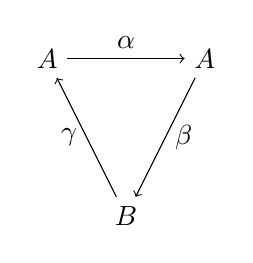
\begin{tikzpicture}
					\node (A) at (-1, 1) {$A$};
					\node (A2) at (1, 1) {$A$};
					\node (B) at (0, -1) {$B$};
					\draw[->] (A) -- node[above]{$\alpha$} (A2);
					\draw[->] (A2) -- node[right]{$\beta$} (B);
					\draw[->] (B) -- node[left]{$\gamma$} (A);
				\end{tikzpicture}
				\caption{Exact couple.}
				\label{fig:exact_couple}
			\end{subfigure}
			\begin{subfigure}{0.49\textwidth}
				\centering
				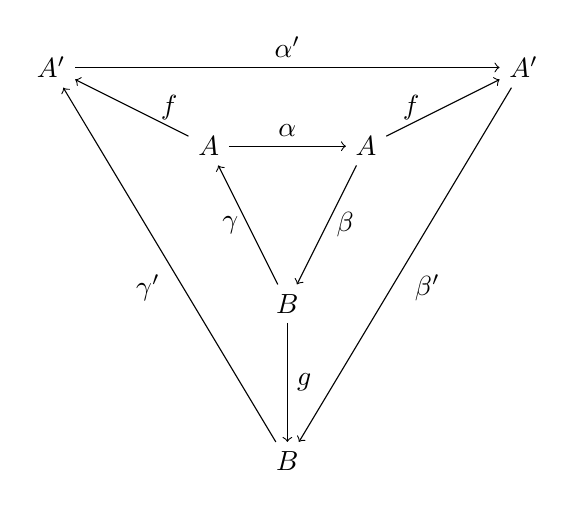
\begin{tikzpicture}
					\node (A') at (-3, 3) {$A'$};
					\node (A2') at (3, 3) {$A'$};
					\node (B) at (0, 0) {$B$};
					\node (A) at (-1, 2) {$A$};
					\node (A2) at (1, 2) {$A$};
					\node (B') at (0, -2) {$B$};
					\draw[->] (A') -- node[above]{$\alpha'$} (A2');
					\draw[->] (A2') -- node[below right]{$\beta'$} (B');
					\draw[->] (B') -- node[below left]{$\gamma'$} (A');
					\draw[->] (A) -- node[above]{$\alpha$} (A2);
					\draw[->] (A2) -- node[right]{$\beta$} (B);
					\draw[->] (B) -- node[left]{$\gamma$} (A);
					\draw[->] (A) -- node[right, xshift=7pt]{$f$} (A');
					\draw[->] (A2) -- node[left, xshift=-5pt]{$f$} (A2');
					\draw[->] (B) -- node[right]{$g$} (B');
				\end{tikzpicture}
				\caption{Morphism of exact couples.}
				\label{fig:exact_couple_morphism}
			\end{subfigure}
			\caption{Category of exact couples.}
			\label{fig:exact_couples_category}
		\end{figure}
	}
	From any exact couple $(A,B,\alpha,\beta,\gamma)$ one can construct a spectral sequence using the following prescription:
	\begin{align}
		E_0 &:= B\\
		d_0 &:= \beta\circ\gamma\\
		&\nonumber\\
        &\ \vdots\nonumber\\
        &\nonumber\\
		E_n &:= \frac{\gamma^{-1}(\alpha^n(A))}{\beta(\alpha^{-n}(0))}\\
		d_n &:= \beta\circ\alpha^{-n}\circ\gamma
	\end{align}
	It is not hard to see that $E_{n+1}=H(E_n,d_n)$, so this construction gives a functor from the category of exact couples to the category of spectral sequences. The higher exact couples $(\alpha^nD,E_n,\ldots)$ are sometimes called \textbf{derived couples}.

	One can also define the term $E_\infty$ using the following limit procedure. For every $n$, take the elements in $E_n$ that are closed under $d_n$ and call these $E_{n,n+1}$. Since there exists a canonical surjection $E_{n,n+1}\rightarrow E_{n+1}$, one can then look at all the elements in $E_{n,n+1}$ for which the image in $E_{n+1}$ is closed under $d_{n+1}$. Call the set of these elements $E_{n,n+2}$. The elements that remain after taking the limit of this operation form the set $E_{n,\infty}$. Now, take the direct limit of the $E_{n,\infty}$ to obtain $E_\infty$. This is equivalent to
	\begin{gather}
		E_\infty := \frac{\cap_i Z(E_i)}{\cup_i B(E_i)},
	\end{gather}
	i.e.~$E_\infty$ contains the equivalence classes of elements that are cycles for all $d_n$ but boundaries for none. If $E_\infty$ is the associated graded object of some filtered object $G$, one says that the spectral sequence \textbf{converges} to $G$.

	Now, consider a differential object $(C,d)$ together with a filtration $\{F_pC\}_{p\in\mathbb{N}}$. Definition \ref{set:filtration} of a filtration immediately gives a short exact sequence for every $p\in\mathbb{N}$:
	\begin{gather}
		0\longrightarrow F_{p-1}C\longrightarrow F_pC\longrightarrow F_pC/F_{p-1}C\longrightarrow 0.
	\end{gather}
	This short sequence in turn gives rise to a long exact sequence in homology, which can be expressed as an exact triangle, and this triangle further leads to an exact couple:
	\begin{gather}
		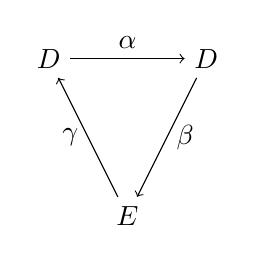
\begin{tikzpicture}
			\node (A) at (-1, 1) {$D$};
			\node (A2) at (1, 1) {$D$};
			\node (B) at (0, -1) {$E$};
			\draw[->] (A) -- node[above]{$\alpha$} (A2);
			\draw[->] (A2) -- node[right]{$\beta$} (B);
			\draw[->] (B) -- node[left]{$\gamma$} (A);
		\end{tikzpicture}
	\end{gather}
	where $D_p = H(F_pC)$ and $E_p=H(F_pC/F_{p-1}C)$. From a more abstract, yet more useful, point of view one can consider the object $E$ as a functor from the category of filtered (differential) objects to the category of graded objects. As such it is constructed from the composition of the homology functor $H$ and the \textit{associated graded object}-functor \[\mathrm{Gr}:C\mapsto\Big\{G_pC := F_pC/F_{p-1}C\Big\}_{p\in\mathbb{N}}.\]

	On the other hand, one could of course also construct the composition $\mathrm{Gr}\circ H$ that first maps a differential object to its homology object and then builds the graded object associated to the filtration \[F_pH(C):=\im\left(H(F_pC)\rightarrow H(C)\right).\] Some straightforward questions can arise at this point: ``\textit{How are the functors $H\circ\mathrm{Gr}$ and $\mathrm{Gr}\circ H$ related?}'', ``\textit{Do they coincide?}'', ... The latter question is easy to answer: ``\textit{No, they do not.}'' However, they can be related and this exactly happens through a spectral sequence that says how the homology of the graded object associated to $C$ can be related to the homology of $C$ itself.

\subsection{Filtered complexes}

	For the remainder of this section only graded differential objects will be considered, i.e.~$(C_\bullet,d_\bullet)=(\{C_p\}_{p\in\mathbb{Z}},d)$ such that $dC_p\subseteq C_p$. In this case the exact couple consist of $D_{p,q}:=H_q(F_pC_\bullet)$ and $E_{p,q}:=H_q(G_pC_\bullet)$ and, consequently, the objects are bigraded. The filtration is also required to be compatible with the differential, i.e.~$dF_iC_j\subseteq F_iC_{j-1}$.

	\sremark{In contrast to most of the literature, the \textit{complementary convention}, i.e.~the convention where $p+q$ denotes the total degree and hence $E_{p,q}=H_{p+q}(G_pC_\bullet)$, is not adopted.}

	Before introducing an expression for a general page $E_r$, the terms of degree zero and one are considered to get some intuition. The differential on $E_0$ is given by
	\begin{gather}
		d_0:\frac{F_pC_q}{F_{p-1}C_q}\rightarrow\frac{F_pC_{q-1}}{F_{p-1}C_{q-1}}
	\end{gather}
	and is induced by the differential $d$ on $C_\bullet$. The kernel of this map is clearly given by all elements $x\in F_pC_q$ such that $dx = 0\mod F_{p-1}C_{q-1}$ (with the additional remark that one also has to take the quotient by $F_{p-1}C_q$). As a result one finds that the homology $E_1=H(E_0, d_0)$ is given by
	\begin{gather}
		E_1^{p,q}:=\frac{\{x\in F_pC_q\mid dx\in F_{p-1}C_{q-1}\}}{F_{p-1}C_q+dF_pC_{q+1}}.
	\end{gather}
	The first term in the denominator was already explained above. The second term comes from the $\im(d_0)$-part in the definition of $H(E_0,d_0)$. One might suspect that some data is missing since the relevant map $d_0^{p, q+1}$ goes from $\frac{F_pC_{q+1}}{F_{p-1}C_{q+1}}$ to $\frac{F_pC_q}{F_{p-1}C_{q}}$. However, the image of $F_{p-1}C_{q+1}$ is a subspace of $F_{p-1}C_q$ and this is already included in the first term, so one might as well work with all of $F_pC_{q+1}$.

	For arbitrary $r>0$, one defines the page $E_r$ as follows:
	\begin{gather}
    	E_r^{p,q}:=\frac{\{x\in F_pC_q\mid dx\in F_{p-r}C_{q-1}\}}{F_{p-1}C_q+dF_{p+r-1}C_{q+1}}.
	\end{gather}

    To relate this more to the usual notions of (co)homology, one can rephrase this in terms of (co)chains, (co)cycles and (co)boundaries. Consider again a filtered complex $F_\bullet C_\bullet$. The following definitions are used:
    \begin{itemize}
        \item The elements of $G_pC_q$ are called the $(p,q)$-\textbf{chains} (in filtering degree $p$).
        \item The elements of \[Z^r_{p,q} := \{c\in G_pC_q\mid dc=0\bmod F_{p-r}C_{q-1}\}\] are called $r$-\textbf{almost} $(p,q)$-\textbf{cycles}.
        \item The elements of \[B^r_{p,q} := dF_{p+r-1}C_{q+1}\] are called $r$-\textbf{almost} $(p,q)$-\textbf{boundaries}.
    \end{itemize}
    It is then easy to see that the page $E^r$ satisfies
    \begin{gather}
        E^r_{p,q} = Z^r_{p,q}/B^r_{p,q},
    \end{gather}
    i.e.~the homology is given by the quotient of the cycles by the boundaries. All these objects fit in a nice sequence of inclusions:
    \begin{gather}
        B^0_{p,q}\hookrightarrow\cdots\hookrightarrow B^\infty_{p,q}\hookrightarrow Z^\infty_{p,q}\hookrightarrow\cdots\hookrightarrow Z^0_{p,q}.
    \end{gather}

\subsection{Convergence}

    \newdef{Limit term}{\index{limit}
        Consider a spectral sequence $\{E^r_{p,q}\}$. If there exists a for every two integers $p,q\in\mathbb{Z}$ an integer $r(p,q)\in\mathbb{N}$ such that for all $r\geq r(p,q)$:
        \begin{gather}
            E^r_{p,q}\cong E^{r(p,q)}_{p,q},
        \end{gather}
        the object $E^\infty:=\{E^{r(p,q)}_{p,q}\}$ is called the \textbf{limit term} and the sequence is said to \textbf{abut} to $E^\infty$.
    }
    \begin{example}[Collapsing sequence]
        If there exists an integer $r\in\mathbb{N}$ such that for all $s\geq r:d_s=0$, the sequence is said to \textbf{collapse} at $r$ and $E^r$ is a limit term. A common example is where the nonvanishing elements of a term are concentrated in a single row or column.
    \end{example}

    \newdef{Convergence}{\index{convergence}
        A spectral sequence ${E^r_{p,q}}$ is said to converge to a graded object $H_\bullet$ with filtering $F_\bullet H_\bullet$, denoted by \[E^r_{p,q}\Rightarrow H_\bullet,\] if
        \begin{gather}
            E^\infty_{p,q}\cong G_p H_q\qquad\qquad\forall p,q\in\mathbb{Z}.
        \end{gather}
    }

    \newdef{Bounded sequence}{\index{bounded!sequence}
        A spectral sequence is said to be bounded if for all numbers $n,r\in\mathbb{Z}$, there only exists a finite number of nonvanishing elements of the form $E^r_{k,n-k}$. A common example are the \textbf{first quadrant spectral sequences} where the only nonvanishing elements have $p,q\geq0$.
    }
    \begin{property}
        Every bounded spectral sequence abuts.
    \end{property}

    \begin{property}[Filtered complex]
        If the spectral sequence of a filtered complex $F_\bullet C_\bullet$, it converges to the chain homology of the complex:
        \begin{gather}
            E^r_{p,q}\Rightarrow H_\bullet(C).
        \end{gather}
    \end{property}

    ?? COMPLETE ??

% \part{Topology}
% \chapter{General Topology}\label{chapter:topology}

    \minitoc

\section{Topological spaces}

    \newdef{Topology}{\index{topology}\label{topology:topology}
        Let $X$ be a set and consider a collection of subsets $\tau\subseteq 2^X$. The set $\tau$ is a topology on $X$ if it satisfies the following axioms:
        \begin{enumerate}
            \item $\emptyset\in\tau$ and $X\in\tau$,
            \item $\forall\mathcal{F}\subseteq\tau:\bigcup_{V\in\mathcal{F}}V \in \tau$, and
            \item $\forall\,U,V\in\tau: U\cap V\in\tau$.
        \end{enumerate}
        The elements of $\tau$ are called \textbf{open sets} and the couple $(X,\tau)$ is called a \textbf{topological space}. \textbf{Closed sets} are defined as the sets that have an open complement. Because complements are uniquely defined, one could just as well define a topology in terms of closed subsets.
    }

    \begin{property}[\difficult{Category of opens}]
        Consider a topological space $(X,\tau)$ and let $U\subseteq V\in\tau$. The topology $\tau$ together with the collection of inclusion maps $U\hookrightarrow V$ forms a poset and, by extension, a small category $\symbfsf{Open}(X)$.
    \end{property}

    \newdef{Pointed topological space}{\label{topology:pointed_space}\index{pointed!topological space}
        A topological space $X$ with a designated \textbf{base point} $x_0\in X$. Equivalently, a pointed object (\cref{cat:pointed_object}) in the category $\symbfsf{Top}$ of topological spaces.
    }

    \begin{example}[Relative topology\footnotemark]\label{topology:relative_topology}
        \footnotetext{Sometimes called the \textbf{subspace} or \textbf{trace topology}.}
        Any subset $Y$ of a topological space $(X,\tau)$ can be turned into a topological space by equipping it with the following topology:
        \begin{gather}
            \tau_{\text{rel}} := \{U_i\cap Y\mid U_i\in\tau\}\,.
        \end{gather}
    \end{example}
    \begin{example}[Discrete topology]\index{discrete!topology}
        The topology in which every subset is open (and thus also closed).
    \end{example}
    \begin{example}[Indiscrete topology]
        The topology in which only the empty set and the space itself are open.
    \end{example}

    \newdef{Interior}{\index{interior}
        The interior $Y^\circ$ of a subset $Y$ of a topological space $X$ is defined as the union of all open subsets of $Y$. Elements of the interior are called \textbf{interior points} of $Y$.
    }
    \newdef{Closure}{\index{closure}
        The closure $\overline{Y}$ of a subset $Y$ of a topological space $X$ is defined as the intersection of all closed sets containing $Y$.
    }
    \newdef{Boundary}{\index{boundary}
        The boundary $\partial Y$ of a subset $Y$ of a topological space $X$ is defined as $\overline{Y}\backslash Y^\circ$.
    }

    \newdef{Borel algebra}{\index{Borel!set}\label{topology:borel_set}
        The $\sigma$-algebra \ref{set:sigma_algebra} generated by all open subsets of a topological space. The elements of this $\sigma$-algebra are called Borel sets.
    }
    \begin{property}
        The closed subsets of a topological space also generate the Borel $\sigma$-algebra.
    \end{property}

    \newdef{Topological group}{\index{group!topological}
        A group equipped with a topology such that both the multiplication and inversion morphisms are continuous.
    }

    \newdef{$G_\delta$-set}{\index{G$_\delta$-set}\label{top:g_delta}
        A countable intersection of open sets.
    }
    \newdef{$F_\sigma$-set}{\index{F$_\sigma$-set}
        A countable union of closed sets.
    }

\subsection{Neighbourhoods}

    \newdef{Neighbourhood}{\index{neighbourhood}
        A set $N\subseteq X$ is a neighbourhood of a point $x\in X$ if there exists an open set $U$ such that $x\in U\subseteq N$.
    }

    Although the following two notions are often treated as synonyms in the literature, they can be given a separate meaning.
    \newdef{Limit point}{\index{limit!point}
        Let $Y$ be a subset of $X$. A point $x\in X$ is a limit point of $Y$ if every neighbourhood of $x$ contains at least one point of $Y$ different from $x$.
    }
    \newdef{Adherent point}{\index{adherent point}
        Let $Y$ be a subset of $X$. A point $x\in X$ is an adherent point of $Y$ if every neighbourhood of $x$ contains at least one point of $Y$. A point $x$ is an adherent point of $Y$ if and only if it is an element of the closure $\overline{Y}$.
    }

    \newdef{Accumulation point\footnotemark}{\index{accumulation point|seealso{limit point}}
        \footnotetext{Sometimes called a \textbf{cluster point}.}
        Let $x\in X$ be a limit point of $Y$. It is called an accumulation point of $Y$ if every open neighbourhood of $x$ contains infinitely many points of $Y$.
    }

    \newdef{Basis}{\index{basis}
        A collection $\mathcal{B}\subseteq\tau$ of open subsets of a topological space $(X,\tau)$ is called a basis for $\tau$ if every $U\in\tau$ can be written as
        \begin{gather}
            U = \bigcup_{V\in\mathcal{F}}V\,,
        \end{gather}
        for some $\mathcal{F}\subseteq\mathcal{B}$.
    }
    \newdef{Local basis}{
        A collection $\mathcal{B}_x$ of open neighbourhoods of a point $x\in X$ is a local basis of $x$ if every neighbourhood of $x$ contains at least one element in $\mathcal{B}_x$.
    }

    \newdef{First-countable space}{\index{countability axiom}
        A topological space $(X,\tau)$ for which, for every point $x\in X$, there exists a countable local basis.
    }
    \begin{property}[Decreasing basis]
        Let $x\in X$. If there exists a countable local basis for $x$, there also exists a countable decreasing local basis for $x$.
    \end{property}

    \newdef{Second-countable space}{
        A topological space $(X,\tau)$ for which there exists a countable (global) basis.
    }

    \begin{property}[Closure]\label{topology:closure}
        Let $X$ be a topological space. The closure of a subset $Y\subseteq X$ is given by
        \begin{gather}
            \overline{Y} = \{x\in X\mid\exists\text{ a net }\net{x}\text{ in } X:x_\alpha\longrightarrow x\}.
        \end{gather}
        This implies that the topology on $X$ is completely determined by the convergence of nets (\cref{set:net}).
    \end{property}

    \newdef{Fr\'echet--Urysohn space}{\index{Fr\'echet--Urysohn space}\index{sequential!space}\index{Fr\'echet--Urysohn space|see{sequential space}}
        A topological space for which the closure of every subset is equal to its sequential closure, i.e.~the subset obtained as in \cref{topology:closure}, but with nets replaced by sequences.

        Fr\'echet--Urysohn spaces form an important subclass of \textbf{sequential spaces}, i.e.~topological spaces where the topology is uniquely determined by the convergence of sequences: a subset of a sequential space is closed if and only if every convergent sequence converges to a point in the set.
    }
    The following property is of great practical importance.
    \begin{property}\label{topology:first_countable_sequential}
        Every first-countable space is Fr\'echet--Urysohn and, therefore, only convergent sequences have to be considered in these spaces.
    \end{property}

    \newdef{Germ}{\index{germ}\label{topology:germ}
        Let $X$ be a topological space and let $Y$ be a set. Consider two functions $f,g:X\rightarrow Y$. If there exists a neighbourhood $N$ of a point $x\in X$ such that
        \begin{gather}
            f(u) = g(u)\qquad\qquad\forall u\in N\,,
        \end{gather}
        then this property defines an equivalence relation denoted by $f\sim_x g$ and the equivalence classes are called germs at $x$.
    }

\subsection{Separation axioms}\index{separation!axioms}

    \newdef{Irreducible space}{\index{irreducible!space}
        A topological space that is not the union of two proper closed subsets or, equivalently, if the intersection of two nonempty open subsets is again nonempty.
    }

    \newdef{$T_0$-space}{\index{distinguishable}\index{Kolmogorov|seealso{topology}}\index{topology!Kolmogorov}
        A topological space such that for every two distinct points at least one of them has a neighbourhood not containing the other, i.e.~they are \textbf{topologically distinguishable}. $T_0$-spaces are also said to carry a \textbf{Kolmogorov topology}.
    }

    \newdef{$T_1$-space}{\index{separated}\index{Fr\'echet|seealso{topology}}\index{topology!Fr \'echet}
        A topological space such that for every two distinct points $x,y$ there exists neighbourhood $N,N'$ of $x$ and $y$ respectively such that $y\not\in N$ and $x\not\in N'$, i.e.~they can topologically \textbf{separated}. $T_1$-spaces are also said to carry a \textbf{Fr\'echet topology} (not to be confused with \textit{Fr\'echet spaces} from functional analysis).
    }

    \newdef{Hausdorff space}{\index{Hausdorff!space}\label{topology:hausdorff}
        A topological space $X$ is called a Hausdorff space or $T_2$-space if it satisfies the following condition:
        \begin{gather}
            \forall x,y\in X:\exists\text{ neighbourhoods }N\ni x,N'\ni y:N\cap N'=\emptyset\,.
        \end{gather}
        The points are said to be \textbf{separated by neighbourhoods}. It can be shown that this definition is equivalent to requiring that the diagonal $\Delta_X$ is closed in the product space $X\times X$.
    }
    \begin{property}[Closed points]
        Every singleton and, by extension, every finite subset of a Hausdorff space is closed.
    \end{property}

    \newdef{Urysohn space}{\index{Urysohn!space}
        A topological space is called an Urysohn space or $T_{2\sfrac{1}{2}}$-space if every two distinct points can be separated by closed neighbourhoods.
    }

    \newdef{Regular space}{\index{regular}\label{topology:regular}
        A topological space such that for every closed subset $V$ and every point $x\not\in V$ there exist disjoint open subsets $U,U'$ such that $x\in U$ and $V\subset U'$.
    }
    \newdef{$T_3$-space}{
        A space that is both regular and $T_0$.
    }

    \newdef{Normal space}{\index{normal}\label{topology:normal}
        A topological space such that every two closed subsets have disjoint neighbourhoods.
    }
    \newdef{$T_4$-space}{
        A space that is both normal and $T_1$.
    }

    \begin{property}[Nesting of axioms]
        A space satisfying the separation axiom $T_k$ also satisfies all separation axioms $T_{i\leq k}$.
    \end{property}

\subsection{Convergence}

    \newdef{Convergence}{\index{convergence}
        A sequence $\seq{x}$ in $X$ is said to (\textbf{sequentially}) converge to a point $x\in X$ if
        \begin{gather}
            \forall\text{ neighbourhoods }U\text{ of }x:\exists N\in\mathbb{N}_0:\forall n>N:x_n\in U\,.
        \end{gather}
    }

    \begin{property}[Uniqueness]\label{topology:hausdorff_limit}
        The limit of a convergent sequence in a Hausdorff space is unique.
    \end{property}

    \begin{property}[Subsequences]
        Every subsequence of a convergent sequence converges as well. Moreover, in a Hausdorff space, the limits coincide.
    \end{property}

\section{Morphisms}
\subsection{Continuity}

    \newdef{Continuous function}{\index{continuity}
        A function between topological spaces for which the preimage of every open set is also open.
    }
    \begin{notation}
        The set of all continuous functions between two topological spaces $X,Y$ is often denoted by $C(X,Y)$.
    \end{notation}

    \newdef{Initial topology}{\index{topology!initial}\index{topology!limit|see{initial}}\label{topology:initial_topology}
        Consider a collection of functions $\{f_i:X\rightarrow Y_i\}_{i\in I}$ between topological spaces. The initial (or \textbf{limit}) topology on $X$, with respect to this family, is the coarsest topology on $X$ for which all maps $f_i$ are continuous.
    }
    \newdef{Final topology}{\index{topology!final}\label{topology:final_topology}
        Consider a collection of functions $\{f_i:Y_i\rightarrow X\}_{i\in I}$ between topological spaces. The final (or \textbf{inductive}\footnote{The reason for this name is that the direct (or inductive) limit (\cref{set:direct_limit}) of topological spaces is usually endowed with this topology.}) topology on $X$, with respect to this family, is the finest topology on $X$ for which all maps $f_i$ are continuous.
    }

    \begin{property}[Sequential continuity]\label{topology:sequential_continuity}
        Consider a function $f:X\rightarrow Y$ of topological spaces, where $X$ is first-countable. The following statements are equivalent:
        \begin{itemize}
            \item $f$ is continuous.
            \item The sequence $(f(x_n))_{n\in\mathbb{N}}$ converges to $f(a)\in Y$ whenever the sequence $\seq{x}$ converges to $a\in X$.
        \end{itemize}
    \end{property}
    \begin{remark}
       If the space $Y$ in the previous theorem is Hausdorff, the limit is irrelevant since it is unique by \cref{topology:hausdorff_limit} above.
    \end{remark}
    \begin{remark}
        If the space $X$ is not first-countable, one has to consider the convergence of nets (\cref{set:net}).
    \end{remark}

    \begin{theorem}[Urysohn's lemma]\index{Urysohn!lemma}\label{topology:urysohns_lemma}
        A topological space X is normal if and only if every two closed disjoint subsets $A, B\subset X$ can be separated by a continuous function $f:X\rightarrow [0,1]$, i.e.~$\forall a\in A,b\in B$ there exists a continuous function $f:X\rightarrow [0,1]$ such that
        \begin{gather}
            f(a) = 0\qquad\text{and}\qquad f(b) = 1\,.
        \end{gather}
    \end{theorem}

    The following, seemingly unrelated, theorem is actually equivalent to Urysohn's lemma.
    \begin{theorem}[Tietze extension theorem]\index{Tietze extension theorem}
        Consider a continuous function $f:V\rightarrow\mathbb{R}$, where $V$ is a closed subset of a normal space $X$. There exists a continuous function $F:X\rightarrow\mathbb{R}$ such that $\forall x\in V:F(x) = f(x)$. Furthermore, if the function $f$ is bounded, then $F$ can be chosen to be bounded by the same number.
    \end{theorem}

    \newdef{Limit superior and inferior}{\index{limit}\label{topology:limit_superior}
        Consider a continuous function $f:X\rightarrow\mathbb{R}$. The limit inferior and superior of $f$ at $x_0\in(X,\tau)$ are defined as follows:
        \begin{align}
            \liminf_{x\rightarrow x_0}f(x) &:= \sup\bigl\{\inf\{f(x)\mid x\in U\backslash\{x_0\}\}\bigm\vert U\in\tau,x_0\in U,U\backslash\{x_0\}\neq\emptyset\}\bigr\}\,,\\
            \limsup_{x\rightarrow x_0}f(x) &:= \inf\bigl\{\sup\{f(x)\mid x\in U\backslash\{x_0\}\}\bigm\vert U\in\tau,x_0\in U,U\backslash\{x_0\}\neq\emptyset\}\bigr\}\,.
        \end{align}
        For functions on a subspace $Y\subset X$ one should look at the values $\{f(x)\mid x\in Y\cap U\backslash\{x_0\}\}$. For the definition to make sense, $x_0$ should be a limit point of $Y$.
    }
    \newdef{Semicontinuity}{\index{semi-!continuity}\label{topology:semicontinuity}
        Consider a function $f:X\rightarrow\overline{\mathbb{R}}$ on a topological space. It is said to be \textbf{upper semicontinuous} at a point $x_0\in X$ if for all $y\in\mathbb{R}$ with $y>f(x_0)$ there exists a neighbourhood of $x_0$ such that $f(x)<y$ for all $x\in U$. Analogously, the function is said to be \textbf{lower semicontinuous} at a point $x_0\in X$ if for all $y\in\mathbb{R}$ with $y<f(x_0)$ there exists a neighbourhood of $x_0$ such that $f(x)>y$ for all $x\in U$.

        These definitions can be expressed more succintly as follows:
        \begin{itemize}
            \item Upper semicontinuous: $\limsup_{x\rightarrow x_0}f(x)\leq f(x_0)$ for all $x_0\in X$, and
            \item Lower semicontinuous: $\liminf_{x\rightarrow x_0}f(x)\geq f(x_0)$ for all $x_0\in X$.
        \end{itemize}
    }

\subsection{Homeomorphisms}

    \newdef{Homeomorphism}{\index{homeomorphism}
        A bijection $f$ such that both $f$ and $f^{-1}$ are continuous.
    }

    \newdef{Embedding}{\index{embedding}\label{topology:embedding}
        A continuous function that is a homeomorphism onto its image.
    }
    \newdef{Local homeomorphism}{\index{local!homeomorphism}\index{etale!morphism}\label{topology:etale_morphism}
        A continuous function $f:X\rightarrow Y$ such that every point $x\in X$ has an open neighbourhood $U$ for which $f|_U$ is an embedding. Local homeomorphisms are also called \textbf{\'etale morphisms}.
    }

    \newdef{Covering space}{\index{covering!space}\label{topology:covering_space}
        Consider two topological spaces $C,X$ and a continuous surjection $p:C\rightarrow X$. $C$ is said to be a covering space of $X$ (and $p$ is called a \textbf{covering map}) if, for all points $x\in X$, there exists an open neighbourhood $U$ of $x$ such that $p^{-1}(U)$ can be written as a disjoint union of open sets in $C$, where every set is mapped homeomorphically onto $U$. The neighbourhoods $U$ are sometimes said to be \textbf{evenly covered}.
    }
    \begin{notation}
        Because the covering map $p:C\rightarrow M$ is surjective, the space $M$ can be left implicit. Therefore, covering spaces are often just denoted by the couple $(C,p)$.
    \end{notation}

    \newdef{Covering transformation}{\label{topology:covering_transformation}
        Consider two covering spaces $(C,p)$ and $(C',p')$. A continuous function $f:C\rightarrow C'$ is called a covering transformation if $p'\circ f=p$.
    }

    \newdef{Deck transformation}{\index{deck transformation}\label{topology:deck_transformation}
        Let $p:C\rightarrow X$ be a covering map. The automorphism group of $(C,p)$ in the category of covering spaces (over $X$) is given by all homeomorphisms $\varphi$ satisfying $p\circ\varphi=p$. These automorphisms are called deck transformations.
    }

    \newdef{\'Etale space}{\index{etale!space}\index{stalk}\label{topology:etale_space}
        Let $X$ be a topological space. A topological space $Y$ is called an \'etale space over $X$ if there exists a surjective local homeomorphism $\pi:Y\rightarrow X$. The preimage $\pi^{-1}(x)$ of a point $x\in X$ is called the \textbf{stalk} of $\pi$ over $x$.
    }
    \begin{example}
        Every covering space is an \'etale space.
    \end{example}

    \newdef{\difficult{Pseudogroup}}{\index{pseudo-!group}\label{topology:pseudogroup}
        Let $(X,\tau)$ be a topological space. A pseudogroup is a collection $\mathcal{G}$ of homeomorphisms $\phi:U\rightarrow V$ between open subsets of $X$ such that:
        \begin{enumerate}
            \item $\mathbbm{1}_U\in\mathcal{G}$ for all $U\in\tau$.
            \item If $\phi\in\mathcal{G}$, then $\phi^{-1}\in\mathcal{G}$.
            \item If $V\subset U\in\tau$, then $\phi|_V\in\mathcal{G}$.
            \item If $U=\bigcup_{i\in I}U_i$ and $\phi|_{U_i}:U_i\rightarrow V$ is an element of $\mathcal{G}$ for all $i\in I$, then $\phi\in\mathcal{G}$.
            \item If $\phi:U\rightarrow V$ and $\psi:U'\rightarrow V'$ are elements of $\mathcal{G}$ and $V\cap U'\neq\emptyset$, then $\psi\circ\phi|_{\phi^{-1}(V\cap U')}\in\mathcal{G}$.
        \end{enumerate}
    }

\section{Associated constructions}

    \begin{construct}[Product topology]\index{product!topology}\index{Tychonoff!topology}\label{topology:tychonoff_topology}
        First, consider the case with only a finite number of spaces $\{(X_i,\tau_i)\}_{i\in I}$. The Cartesian product $X:=\prod_{i\in I}X_i$ can be turned into a topological space by equipping it with the topology generated by the following basis:
        \begin{gather}
            \mathcal{B} := \left\{\prod_{i\in I}U_i\,\middle\vert\,U_i\in\tau_i\right\}.
        \end{gather}
        In the general case the topology can be defined using the canonical projections $\pi_i:X\rightarrow X_i$. The general product topology, called the \textbf{Tychonoff topology}, is the initial topology with respect to the projections $\pi_i$.
    \end{construct}

    \begin{construct}[Disjoint union]\index{disjoint union}\label{topology:disjoint_union}
        Let $\{(X_i,\tau_i)\}_{i\in I}$ be a family of topological spaces and consider the disjoint union
        \begin{gather}
            X := \bigsqcup_{i\in I}X_i
        \end{gather}
        together with the canonical inclusion maps $\phi_i:X_i\rightarrow X:x_i\mapsto(i,x_i)$. The set $X$ can be turned into a topological space by equipping it with the following topology:
        \begin{gather}
            \tau_X := \bigl\{U\subseteq X\bigm\vert\forall i\in I:\phi_i^{-1}(U)\in\tau_i\bigr\}\,.
        \end{gather}
    \end{construct}

    \begin{construct}[Quotient space]\index{quotient!space}\label{topology:quotient_space}
        Consider a topological space $(X,\tau)$ and a subset $Y\subseteq X$. The quotient $X/Y$ is defined as the set $X\backslash Y\sqcup\{\ast\}$ where the point $\ast$ can be regarded as the result of identifying all points in $Y$. This canonically turns the quotient space into a pointed space.

        Let $\pi$ be the canonical projection $X\rightarrow X/Y$. The quotient space can be turned into a topological space by equipping it with the following topology:
        \begin{gather}
            \tau_Q := \bigl\{U\subseteq X/Y\bigm\vert\pi^{-1}(U)\in\tau\bigr\}\,.
        \end{gather}
    \end{construct}
    \begin{remark}[Degenerate quotient]
        For the degenerate case $Y=\emptyset$ one can also apply the above definition. However, this has the awkward effect that it adjoins a new point to the space $X$ instead of a collapsing it:
        \begin{gather}
            \label{topology:empty_quotient}
            X/\emptyset = X\sqcup\ast\,.
        \end{gather}
    \end{remark}

    \begin{construct}[Wedge sum]\index{wedge!sum}
        Consider two pointed spaces $(X,x_0)$ and $(Y,y_0)$. The wedge sum $X\vee Y$ is defined as the quotient of the disjoint union $X\sqcup Y$ obtained by identifying the basepoints $x_0\sim y_0$.
    \end{construct}
    \newdef{Smash product}{\index{smash product}
        Consider two pointed topological spaces $(X,x_0)$ and $(Y,y_0)$. The smash product $X\wedge Y$ is defined as the quotient
        \begin{gather}
            X\wedge Y := (X\times Y)/(X\vee Y)\,,
        \end{gather}
        where $X\vee Y$ sits inside the product as the union of $X\times\{y_0\}$ and $\{x_0\}\times Y$.
    }

    \begin{construct}[Suspension]\index{suspension}\label{topology:suspension}
        Let $X$ be a topological space. The suspension of $X$ is defined as the following quotient space:
        \begin{gather}
            SX := (X\times [0,1])/\bigl\{(x,0)\sim (y,0)\text{ and }(x,1)\sim (y,1)\bigm\vert x,y\in X\bigr\}\,.
        \end{gather}
        By the remark about degenerate quotients the suspension of the empty set is in fact not empty, but equal to the two-point space $S^0$.

        An often more interesting construction is the \textbf{reduced suspension} $\Sigma X$. This is obtained by taking the ordinary suspension $SX$ of a pointed space $(X,x_0)$ and identifying all copies of $x_0$:
        \begin{gather}
            \Sigma X := SX/(x_0\times[0,1])\,.
        \end{gather}
        An equivalent definition of the reduced suspension can be given in terms of the smash product:
        \begin{gather}
            \Sigma X\cong X\wedge S^1\,.
        \end{gather}
    \end{construct}
    \begin{example}[Spheres]\label{topology:sphere_suspension}
        Up to homeomorphism, the spheres are related by (reduced) suspensions:
        \begin{gather}
            SS^n\cong S^{n+1}\cong\Sigma S^n\,.
        \end{gather}
        If one identifies the empty set with the $(-1)$-sphere, this relation can be continued to the case $n=-1$.
    \end{example}

    \begin{construct}[Attaching space]\index{attaching space}\label{topology:attaching_space}
        Let $X,Y$ be two topological spaces and consider a subspace $A\subseteq X$. For every continuous function $f:A\rightarrow Y$, called the \textbf{attaching map}, one can construct the attaching space or \textbf{adjunction space} $X\cup_f Y$ in the following way:
        \begin{gather}
            X\cup_f Y := (X\sqcup Y)/\{A\sim f(A)\}\,.
        \end{gather}
        In categorical terms, it is the pushout (\cref{cat:pushout}) in $\symbfsf{Top}$ of the inclusion $\iota:A\hookrightarrow X$ along $f:A\rightarrow Y$.
    \end{construct}

    \begin{construct}[Join]\index{join}\label{topology:join}
        Let $\{X_i\}_{i\leq n}$ be a finite collection of topological spaces. The join $X:=X_1\circ\cdots\circ X_n$ is defined as follows. Every point of $X$ is defined by the following data:
        \begin{enumerate}
            \item An element of the standard $n$-simplex (\cref{topology:simplex}), i.e.~an $n$-tuple of nonnegative numbers $\{t_i\}_{i\leq n}$ satisfying $\sum_it_i=1$.
            \item For each index $i$ such that $t_i\neq 0$, a point $x_i\in X_i$.
        \end{enumerate}
        This point in $X$ is denoted by $t_1x_1\oplus\cdots\oplus t_nx_n$.

        In the case of two spaces, there exists a more intuitive construction. Let $X,Y$ be two topological spaces. The join $X\circ Y$ is equal to the quotient space $(X\times Y\times[0,1])/\sim$, where the equivalence relation is defined as follows:
        \begin{itemize}
            \item For all $x\in X$ and $y,y'\in Y$: $(x,y,0)\sim(x,y',0)$.
            \item For all $x,x'\in X$ and $y\in Y$: $(x,y,1)\sim(x',y,1)$.
        \end{itemize}
        This can be interpreted as collapsing one end of the cylinder $(X\times Y)\times[0,1]$ to $X$ and the other end to $Y$.
    \end{construct}
    \begin{property}[\difficult{Monoidal structure}]
        The join induces a monoidal structure on the category $\symbfsf{Top}$, where the tensor unit is given by the empty space $\emptyset$.
    \end{property}

\section{Connected spaces}\label{section:connected}

    \newdef{Connected space}{\index{connected!space}\label{topology:connected}
        A topological space that cannot be written as the disjoint union of two nonempty open sets. Equivalently, a space is said to be connected if the only clopen sets are the empty set and the space itself.
    }

    \begin{property}[Locally constant]\index{locally!constant}
        Let $X$ be a connected space and let $f$ be a function on $X$. If $f$ is \textbf{locally constant}, i.e.~for every $x\in X$ there exists a neighbourhood U on which $f$ is constant, then $f$ is constant on all of $X$.
    \end{property}

    \begin{theorem}[Intermediate value theorem]\index{intermediate value theorem}\label{topology:intermediate_value_theorem}
        Let $X$ be a connected space and let $f:X\rightarrow\mathbb{R}$ be a continuous function. If $a,b\in f(X)$, then $\forall c\in\ ]a,b[\ :c\in f(X)$.
    \end{theorem}

    \newdef{Path-connected space\protect\footnotemark}{\index{arc!connected|see{path-connected}}\index{path!connected}
        \footnotetext{A similar notion is that of \textbf{arcwise-connectedness} where the function $\varphi$ is required to be a homeomorphism.}
        Let $X$ be a topological space. If for every two points $x,y\in X$ there exists a continuous function $\varphi:[0,1]\rightarrow X$ (i.e.~a \textbf{path}) such that $\varphi(0)=x$ and $\varphi(1)=y$, the space is said to be path-connected.
    }

    \begin{property}[Path-connected implies connected]
        Every path-connected space is connected. The converse does not hold. A connected and locally path-connected space is path-connected.
    \end{property}

    \begin{remark}[Connected components]\label{topology:connected_components}
        (Path-)connectedness defines an equivalence relation on the space $X$. The equivalence classes are closed in $X$ and form a cover of $X$. The set of path components of $X$ is often denoted by $\pi_0(X)$.
    \end{remark}

\section{Compact spaces}\label{section:compact}
\subsection{Compactness}

    \newdef{Sequentially compact space}{
        A topological space in which every sequence has a convergent subsequence (the sequence itself does not have to be convergent).
    }

    \begin{property}[First-countable spaces]
        A first-countable space is sequentially compact if and only if every countable open cover has a finite subcover.
    \end{property}

    \newdef{Lindel\"of space}{\index{Lindel\"of!space}
        A space for which every open cover has a countable subcover.
    }
    \begin{property}
        Every second-countable space is a Lindel\"of space.
    \end{property}

    \newdef{Finite intersection property}{\index{finite!intersection property}
        A collection $\mathcal{F}\subseteq P(X)$ of subsets has the finite intersection property (FIP) if
        \begin{gather}
            \bigcap_{V\in\mathcal{F}'}V\neq\emptyset
        \end{gather}
        for all finite $\mathcal{F}'\subset\mathcal{F}$.
    }

    \newdef{Locally finite cover}{
        An open cover of a topological space such that every point has a neighbourhood that intersects only finitely many sets in the cover.
    }

    \newdef{Paracompact space}{\index{para-!compact}\label{topology:paracompact}
        A topological space for which every open cover has a locally finite open refinement.
    }
    \begin{property}
        Every paracompact Hausdorff space is normal.
    \end{property}

    \newdef{Partition of unity}{\index{partition!of unity}\label{topology:partition_of_unity}
        A collection $\{f_i:X\rightarrow[0,1]\}_{i\in I}$ of continuous functions such that for every $x\in X$ the following conditions hold:
        \begin{enumerate}
            \item\textbf{Locally finite}: For every neighbourhood $U$ of $x$, the set $\{f_i\mid\mathrm{supp}f_i\cap U\neq\emptyset\}$ is finite.
            \item\textbf{Normalization}: $\sum_{i\in I}f_i(x)=1$.
        \end{enumerate}
        Consider an open cover $\{V_i\}_{i\in I}$ of $X$. If there exists a partition of unity, also indexed by $I$, such that $\text{supp}(\varphi_i)\subseteq U_i$, this partition of unity is said to be \textbf{subordinate} to the given cover.
    }

    \begin{property}[Hausdorff spaces]\label{topology:paracompact_partition_unity}
        A paracompact space is Hausdorff if and only if it admits a partition of unity subordinate to any open cover.
    \end{property}

    \newdef{Numerable open cover}{\index{numerable}\label{topology:numerable_cover}
        An open cover of a topological space is said to be numerable if the space admits a partition of unity subordinate to the given cover.
    }

    \newdef{Compact space}{\index{compact}
        A topological space for which every open cover has a finite subcover.
    }

    \begin{theorem}[Heine--Borel\footnotemark]\index{Heine--Borel}\index{Borel--Lebesgue}\label{topology:heine_borel}
        \footnotetext{Also called the \textbf{Borel--Lebesgue} theorem.}
        If a topological space $X$ is sequentially compact and second-countable, every open cover has a finite subcover and, therefore, $X$ is compact.
    \end{theorem}
    \begin{result}[Real numbers]
        A subset of $\mathbb{R}^n$ is compact if and only if it is closed and bounded.
    \end{result}

    \newdef{Proper function}{\index{proper!function}\label{topology:proper_function}
        A continuous function for which the inverse of every compact set is again compact.
    }

    \begin{theorem}[Tychonoff's theorem]\index{Tychonoff!compactness theorem}
        Any product of compact topological spaces is compact under the (Tychonoff) product topology (\cref{topology:tychonoff_topology}).
    \end{theorem}

    \newdef{Relatively compact space}{\label{topology:relatively_compact}
        A topological space for which its closure is compact.
    }

    \newdef{Locally compact space}{
        A topological space in which every point has a compact neighbourhood.
    }

    \begin{theorem}[Dini]\index{Dini}
        Let $(X,\tau)$ be a compact space and let $\seq{f}$ be a monotone sequence of continuous functions $f_n:X\rightarrow\mathbb{R}$. If $\seq{f}$ converges pointwise to a continuous function, the convergence is uniform.
    \end{theorem}

    \newdef{$\omega$-bounded space}{\index{bounded!space}
        A topological space in which the closure of every countable subset is compact.
    }

    \newdef{Compact-open topology}{\index{topology!compact-open}\label{topology:compact_open_topology}
        Consider the mapping space $C(X,Y)$ between two topological spaces. This space is often endowed with a topology generated by the subbasis of subsets of the form
        \begin{gather}
            U^K := \{f:X\rightarrow Y\mid K\text{ compact}, U\text{ open and } f(K)\subseteq U\}\,.
        \end{gather}
    }
    \begin{property}[Internal hom]\index{mapping!space}\label{topology:internal_hom}
        Consider two topological spaces $X,Y$ with $X$ locally compact and equip the mapping space $C(X,Y)$ with the compact-open topology. The following relation is satisfied for all topological spaces $Z$:
        \begin{gather}
            C(Z\times X,Y)\cong C\bigl(Z,C(X,Y)\bigr)\,,
        \end{gather}
        i.e.~the mapping space $C(X,Y)$ is an internal hom (\cref{cat:internal_hom}) in the category $\symbfsf{Top}$ and, because the topological product is the product in $\symbfsf{Top}$, $C(X,Y)$ is even an exponential object (\cref{cat:exponential_object}). For this reason the mapping spaces $C(X,Y)$ are also sometimes denoted by $Y^X$.
    \end{property}

    \newdef{Proper action}{\index{proper!action}
        Consider a topological group $G$ together with an action $\vartriangleright:G\times X\rightarrow X$ on a topological space $X$. The action is said to be proper if $G\times X\rightarrow X\times X:(g,x)\mapsto(x,g\vartriangleright x)$ is proper (\cref{topology:proper_function}), i.e.~the subset of elements $g\in G$ such that
        \begin{gather}
            g\vartriangleright K\cap K'\neq\emptyset
        \end{gather}
        for compacta $K,K'\subseteq X$ is itself compact.
    }

\subsection{Compactifications}

    \newdef{Dense}{\index{dense}
        A subset $V\subseteq X$ is said to be dense in a topological space $X$ if $\overline{V}=X$.
    }

    \newdef{Generic point}{\index{generic!point}\label{topology:generic_point}
        A point whose closure is the whole space.
    }

    \newdef{Separable space}{\index{separable!space}\label{topology:separable}
        A topological space that contains a countable, dense subset.
    }
    \begin{property}
        Every second-countable space is separable.
    \end{property}

    \newdef{Compactification}{\index{compactification}
        A compact topological space $(X',\tau')$ is a compactification of a topological space $(X,\tau)$ if $X$ is a dense subspace of $X'$.
    }

    \begin{example}
        Standard examples of compactifications are the extended real line $\mathbb{R}\cup\{-\infty,+\infty\}$ and the extended complex plane $\mathbb{C}\cup\{\infty\}$ for the real line and the complex plane, respectively.
    \end{example}
    \begin{remark*}
        It is important to note that compactifications are not necessarily unique.
    \end{remark*}

    \newdef{One-point compactification}{\index{Alexandrov!compactification}\index{compactification}\label{topology:alexandrov_compactification}
        Let $X$ be a Hausdorff space. A one-point compactification or \textbf{Alexandrov compactification} is a compactification $\widehat{X}$ such that $\widehat{X}\backslash X$ is a singleton.
    }
    \begin{example}[Real line]\index{projection!stereographic}
        The classic example of a (one-point) compactification is that of the real line. By adjoining the points $\pm\infty$ and identifying them, the circle $S^1$ is obtained. In general one can obtain the $n$-dimensional sphere $S^n$ as the one-point compactification of $\mathbb{R}^n$. This can be regarded as an inverse \textit{stereographic projection}.
    \end{example}

\section{Uniform spaces}

    \newdef{Uniform structure}{\index{uniform!space}
        A uniform structure on a set $X$ consists of a collection $\mathfrak{U}$ of subsets $U\subseteq X\times X$ that satisfy the following properties:
        \begin{enumerate}
            \item\textbf{Monotonicity}: If $U\in\mathfrak{U}$ and $U\subset V$, then $V\in\mathfrak{U}$.
            \item\textbf{Intersections}: If $U, V\in\mathfrak{U}$, then $U\cap V\in\mathfrak{U}$.
            \item\textbf{Diagonals}: If $U\in\mathfrak{U}$, then $\Delta_X\subset U$.
            \item\textbf{Halving}: If $U\in\mathfrak{U}$, there exists $V\in\mathfrak{U}$ such that $V\circ V\subseteq U$.
            \item\textbf{Transposition}: If $U\in\mathfrak{U}$, then $U^t\in\mathfrak{U}$.
        \end{enumerate}
        $U^t$ denotes the converse (\cref{set:converse}) of $U$ and $\circ$ is the relational composition (\cref{set:relational_composition}) of $V$ and $V$. The elements of the uniformity $\mathfrak{U}$ are called \textbf{entourages}. If $(x,y)\in U$ for some entourage $U\in\mathfrak{U}$, then $x$ and $y$ are said to be \textbf{$U$-close}.
    }
    \remark{The first three conditions imply that a uniform structure is in particular a filter (\cref{set:filter}).}

    \todo{COMPLETE (see Bourbaki)}

\section{Bornological spaces}

    \newdef{Bornology}{\index{bornology}\label{topology:bornology}
        A bornology on a set $X$ is a collection $\mathfrak{b}\subset P(X)$ such that:
        \begin{enumerate}
            \item\textbf{Singletons}: $\forall x\in X:\{x\}\in\mathfrak{b}$.
            \item\textbf{Monotonicity}: $A\in\mathfrak{b},B\subset A\implies B\in\mathfrak{b}$.
            \item\textbf{Union}: $A,B\in\mathfrak{b}\implies A\cup B\in\mathfrak{b}$.
        \end{enumerate}
        The sets in $\mathfrak{b}$ are said to be \textbf{bounded} and the pair $(X,\mathfrak{b})$ is called a \textbf{bornological space}.
    }

    \todo{COMPLETE (see e.g. Rejzner)}

\section{\texorpdfstring{Locales $\clubsuit$}{Locales}}
\subsection{Frames}

    \begin{property}[Opens form a frame]
        Consider the poset $\symbfsf{Open}(X)$ of opens of a topological space $X$. This set is closed under finite intersections (limits) and arbitrary unions (colimits). Furthermore, arbitrary unions distribute over finite intersections:
        \begin{gather}
            V\cap\left(\bigcup_{i\in I}U_i\right) = \bigcup_{i\in I}\left(V\cap U_i\right)\,.
        \end{gather}
        This implies that the poset $\symbfsf{Open}(X)$ is a frame (\cref{set:frame}).
    \end{property}

    \newdef{Locale}{\index{locale}\label{topology:locale}
        The previous property can be used to generalize the notion of topological spaces to include `pointless spaces'. Let \textbf{Frame} denote the category of frames together with frame homomorphisms. The category of locales is defined as its opposite category:
        \begin{gather}
            \symbfsf{Loc} := \symbfsf{Frame}^{\text{op}}\,.
        \end{gather}
    }
    \begin{construct}[From locale to topological space]
        There exists an adjunction
        \begin{gather}
            \symbfsf{Loc}\adj{\iota}{\mathrm{Point}}\symbfsf{Top}\,,
        \end{gather}
        where the right adjoint is defined as follows. Let $L$ be a locale. For a topological space, the points are given by continuous functions $\ast\rightarrow X$ and, hence, by frame morphisms $\symbfsf{Open}(X)\rightarrow1\equiv\Omega_{\text{Frame}}=\{0,1\}$. Generalizing this to locales, one defines the set of points of $L$ as the $\Omega_{\text{Loc}}$-elements:
        \begin{gather}
            \mathrm{Point}(L) := \symbfsf{Loc}(1,L)\,.
        \end{gather}
        This set can be given a topology by declaring for every $U\in L$ the set $\{p\in\mathrm{Point}(L)\mid p^{-1}(U) = 1\}$ to be open.
    \end{construct}

    \newdef{Sober space}{\index{sober}\label{topology:sober_space}
        A topological space $X$ for which the map $X\rightarrow\mathrm{Point}(X)$ is a homeomorphism, i.e.~the points of $X$ are precisely determined by its frame of opens. Equivalently, a topological space such that every irreducible closed subset is the closure of a unique point, i.e.~has a unique generic point (\cref{topology:generic_point}). Important examples are Hausdorff spaces.
    }

\subsection{Stone spaces}\label{section:stone_spaces}

    \newdef{Stone space}{\index{Stone!space}
        The inverse limit (\cref{set:inverse_limit}) of an inverse system of finite, discrete spaces. Equivalently, it is a totally disconnected, compact Hausdorff space (\namecrefs{section:connected}~\ref{section:connected} and~\ref{section:compact}).
    }

    \begin{property}[Stone duality]\index{Stone!duality}\index{pro-!finite set}\index{spectrum}
        By \textit{Stone duality}, these spaces are equivalent to pro-objects (\cref{cat:pro_object}) in the category of finite sets, i.e.~they are equivalent to \textbf{profinite sets}. Moreover, the opposite category of Stone spaces is equivalent to the category of Boolean algebras (\cref{set:boolean}):
        \begin{gather}
            \symbfsf{Bool}\cong\symbfsf{Pro(FinSet)}^{\text{op}}\cong\symbfsf{Stone}^{\text{op}}\,.
        \end{gather}
        The isomorphism between the category of Boolean algebras and Stone spaces is the content of \textbf{Stone's representation theorem}. Every Boolean algebra $B$ is isomorphic to the algebra of clopen subsets of the Stone space $S(B)$, consisting of the ultrafilters on $B$ (\cref{set:ultrafilter}). A topology on $S(B)$ is generated by the sets $\{x\in S(B)\mid b\in x\}$, where $b$ ranges over all elements of $B$. The space $S(B)$ might also be called the \textbf{spectrum} of $B$.
    \end{property}

    \newdef{Profinite group}{\index{group!profinite}\label{topology:profinite_group}
        A Stonean topological group or, equivalently, a group object in the category of profinite sets.
    }
    \newdef{Profinite completion}{\index{completion!profinite}\label{topology:profinite_completion}
        Consider a group $G$. Its profinite completion $\widehat{G}$ is constructed as the inverse limit of the system consisting of the quotient groups $G/N$, where the $N$ are normal subgroups of finite index (\cref{group:index}).
    }

    Although, by Stone duality, pro-objects in the category of finite sets can be identified with their limit (in the category of topological spaces), this is not the case for infinite sets.
    \newdef{Progroup}{\index{pro-!group}\index{Mittag-Leffler condition}
        A pro-object (\cref{cat:pro_object}) in the category of groups. If all morphisms in the underlying system are surjective, the progroup itself is called \textbf{surjective}.\footnote{Surjective progroups are exactly those satisfying the \textit{Mittag-Leffler condition}.}
    }
    \begin{remark}
        Due to the strong relation between locales and topological spaces, there is also a relation between topological groups and localic groups. Because the functor of points $\func{Point}{Loc}{Top}$ is a right adjoint, it preserves limits and, therefore, group objects. This induces a functor $\symbfsf{LocGrp}\rightarrow\symbfsf{TopGrp}$. The converse is, however, not true in general (although it is, for example, true when restricting to locally compact groups).
    \end{remark}

    \begin{property}\index{group!localic}
        Surjective progroups are equivalent to \textbf{localic groups}, i.e.~group objects in $\symbfsf{Loc}$, that are inverse limits of discrete groups (these are also called \textbf{prodiscrete}).
    \end{property}

    Localic groups have a strong connection to \textit{topos theory} (see \labelref{chapter:topos}).
    \begin{property}[Galois topos]\index{Galois!topos}
        Every localic group $G$ gives rise to a classifying topos $\symbfsf{B}G$. Although the functor $\symbfsf{LocGrp}\rightarrow\symbfsf{Topos}$ is not an embedding, it becomes one when restricting to the subcategory of prodiscrete localic groups. The topoi arising in this way are also called \textbf{Galois topoi}.
    \end{property}
% \chapter{Algebraic Topology}\label{chapter:algtop}

    References for this chapter are~\citet{massey_basic_1991,merry_algebraic_2018}.

    \minitoc

\section{Homotopy theory}\label{section:homotopy}
\subsection{Homotopy}

    \newdef{Retraction}{\index{retract}
        Let $X$ be a topological space and let $A\subseteq X$ be a subspace. A continuous function $f:X\rightarrow A$ is called a retraction (and $A$ is called a \textbf{retract} of $X$) if\footnote{It is a retraction of the inclusion map $A\hookrightarrow X$ in the sense of \cref{cat:retract}.}
        \begin{gather}
            f|_A=\mathbbm{1}_A\,.
        \end{gather}
    }
    \newdef{Homotopy}{\index{homotopy}\index{iso-!topy}\label{topology:homotopy}
        Two continuous functions $f,g:X\rightarrow Y$ are said to be homotopic if there exists a continuous function $H:X\times[0,1]\rightarrow Y$ such that $f(x)=H(x,0)$ and $g(x)=H(x,1)$. This relation induces an equivalence relation on $C(X,Y)$ for which the quotient space is denoted by $[X,Y]$. A homotopy $H$ such that $H(\cdot,t)$ is a homeomorphism for all $t\in[0,1]$ is called an \textbf{isotopy}.
    }
    \newdef{Deformation retraction}{\index{deformation}
        Let $X$ be a topological space and let $A\subseteq X$ be a subspace. $A$ is called a deformation retract if there exists a homotopy between the identity function on $X$ and a retraction $f:X\rightarrow A$.
    }

    \newdef{Homotopy type}{\index{homotopy!type}
        Two topological spaces $X$ and $Y$ are said to be \textbf{homotopy equivalent} or to be of the same homotopy type\footnote{The associated equivalence classes are sometimes called \textbf{strong homotopy types} to distinguish them from the homotopy types associated to the \textit{weak equivalences} introduced further on.} if there exist continuous functions $f:X\rightarrow Y$ and $g:Y\rightarrow X$ such that $f\circ g$ is homotopic to $\mathbbm{1}_Y$ and $g\circ f$ is homotopic to $\mathbbm{1}_X$. The maps $f,g$ are called \textbf{homotopy equivalences}.
    }
    \begin{property}[Homeomorphisms]
        Every homeomorphism is a homotopy equivalence.
    \end{property}

    \newdef{Null-homotopic}{
        A continuous function is said to be null-homotopic if it is homotopic to a constant function.
    }
    \newdef{Contractible space}{\index{contractible}\label{topology:contractible_space}
        A topological space for which the identity map is null-homotopic or, equivalently, a space that is homotopy-equivalent to a point.
    }

    \newdef{Good cover}{\index{cover!good}\label{topology:good_cover}
        Let $X$ be a topological space with an open cover $\mathcal{U}\equiv\{U_i\}_{i\in I}$. The cover $\mathcal{U}$ is called a good cover (or \textbf{nice cover}) if every nonempty finite intersection $U_{i_1}\cap\ldots\cap\,U_{i_k}$ is contractible.
    }

    \newprop{Path space}{\index{mapping!space}\label{topology:path_space}
        Consider a topological space $X$. By \cref{topology:internal_hom}, functions $Y\rightarrow X^{[0,1]}$ to the path space represent functions $Y\times[0,1]\rightarrow X$, i.e.~the path space represents homotopies to $X$.
    }

    \newdef{Mapping class group}{\index{mapping class group}\label{topology:MCG}
        Consider a topological space $X$ with some additional structure denoted by $\mathfrak{X}$ (often $\mathfrak{X}$ will be trivial). The mapping class group of $X$ is defined as the quotient
        \begin{gather}
            \mathrm{MCG}(X,\mathfrak{X}) := \Aut(X,\mathfrak{X})\,/\Aut_0(X,\mathfrak{X})\,,
        \end{gather}
        i.e.~as the set of path components of its automorphism group (path are, in this case, given by isotopies).
    }

\subsection{Homotopy groups}

    \newdef{Loop space}{\index{loop!space}\label{topology:loop_space}
        The set of all \textbf{loops} in a pointed topological space, i.e.~all continuous functions $\gamma:(S^1,t_0)\rightarrow(X,x_0)$ for which $\gamma(t_0)=x_0$. This space is denoted by $\Omega_{x_0}X$ (if the base point is clear, the subscript is often omitted). It can be turned into a topological space by equipping it with the compact-open topology (\cref{topology:compact_open_topology}).

        When one drops the requirement of based loops, i.e.~when one considers the space of all continuous functions $S^1\rightarrow X$, the resulting space is called the \textbf{free loop space} on $X$. This space is denoted by $LX$.
    }
    \newdef{Loop group}{\index{loop!group}\label{topology:loop_group}
        In the case of topological groups, one can define a group structure on the (free) loop space. With the compact-open topology, it becomes a topological group.
    }
    \begin{remark}[\difficult{$H$-structure}]\index{H-!space}\label{topology:h_structure}
        Loop spaces can be equipped with a multiplication corresponding to the concatenation of loops\footnote{It should be noted that the rate at which the concatenated loops are traversed is doubled because the parameter $t$ should remain an element of $S^1\cong[0, 1]/_{0\sim1}$.}. However, this operation is not strictly associative and, hence, it does not endow the loop space with a group structure. Instead, it turns the loop space into an \textit{H-group}, which is in particular an $A_\infty$-space (\cref{cat:A_infinity_space}), i.e.~a group up to homotopy.
    \end{remark}

    \newdef{Fundamental group}{\index{fundamental!group}
        The fundamental group $\pi_1(X,x_0)$ is defined as the loop space modulo homotopies, i.e.~$\pi_1(X,x_0):=\pi_0(\Omega_{x_0}X)$, where $\pi_0$ denotes the set of path components (\cref{topology:connected_components}). As the name implies, the fundamental group can be given the structure of a multiplicative group where the operation is inherited from that of the loop space.
    }
    \begin{remark}
        In general, as the notation implies, the fundamental group depends on the base point $x_0$. However, when the space $X$ is path connected, the fundamental groups belonging to different base points are isomorphic. It follows, that one can speak of `the' fundamental group in the case of path-connected spaces.
    \end{remark}

    \begin{property}[Groups]\label{topology:abelian_fundamental_group}
        The fundamental group of a topological group is Abelian. This follows from an Eckmann--Hilton argument (\cref{algebra:eckmann_hilton}).
    \end{property}

    \newdef{Fundamental groupoid $\clubsuit$}{\index{fundamental!groupoid}\index{Poincar\'e!groupoid}\label{topology:fundamental_groupoid}
        Let $X$ be a topological space. The fundamental (or \textbf{Poincar\'e}) groupoid $\symbf{\Pi}_1(X)$ is the groupoid consisting of the following data:
        \begin{itemize}
            \item\textbf{Objects}: $X$, and
            \item\textbf{Morphisms}: Endpoint-preserving homotopy classes of continuous functions $f:[0,1]\rightarrow X$.
        \end{itemize}
        The fundamental group $\pi_1(X,x)$ can be recovered as the automorphism group of $x\in\mathrm{ob}(\symbf{\Pi}_1(X))$.

        This construction can be generalized to an $\infty$\textit{-groupoid} (see \cref{topos:infty_groupoid}), where the class of $k$-morphisms is given by $k$-dimensional `paths'. More explicitly, it is the \textit{Kan complex} (see \cref{model:kan_complex}) given by
        \begin{gather}
            \mathrm{Sing}(X):[k]\mapsto\mathbf{Top}(\Delta^k,X)\,,
        \end{gather}
        the \textit{singular simplicial complex} of $X$ (to be defined in \cref{section:singular_homology}).
    }

    \newdef{Simply-connected space}{\index{simply-connected}\label{topology:simply_connected}
        A topological space that is path connected and whose fundamental group is trivial.
    }
    \newdef{Semilocally simply connected}{
        A topological space in which every point admits a neighbourhood in which every loop can be contracted to a point.
    }

    \newdef{Universal covering space}{\index{universal!covering space}
        A simply-connected covering space (\cref{topology:covering_space}).
    }
    \begin{uproperty}
        Let $X$ be a topological space and let $\widetilde{X}$ be its the universal covering space. Every other covering space of $X$ is also covered by $\widetilde{X}$.
    \end{uproperty}
    \begin{property}[Automorphisms]\index{deck transformation}\label{topology:universal_cover_automorphisms}
        Consider a topological space $X$ and let $\widetilde{X}$ be its universal covering space. The group of deck transformations $\Aut(\widetilde{X})$ (\cref{topology:deck_transformation}) is isomorphic to the fundamental group $\pi_1(X)$. Hence, one obtains
        \begin{gather}
            X\cong\widetilde{X}/\pi_1(X)\,.
        \end{gather}
    \end{property}
    \begin{property}[Existence]
        If the space is connected, locally path-connected and semilocally simply-connected, a universal cover exists.

        An explicit construction for a path-connected space is the following (when multiple path-components exist, one should take the disjoint union of the individual covers):
        \begin{gather}
            \widetilde{X} = \bigl\{[\gamma]\bigm\vert\gamma:[0,1]\rightarrow X,\gamma(0)=x_0\bigr\}\,,
        \end{gather}
        where $x_0$ is the base point of $X$ and $[\gamma]$ denotes the homotopy class of $\gamma$.
    \end{property}
    \begin{result}\label{topology:equivalent_categories}
        This property also implies that, for connected, locally path-connected and semilocally simply-connected spaces, the category of coverings is equivalent to the category of continuous representations of the fundamental group.
    \end{result}

    The definition of fundamental groups can be generalized to arbitrary dimensions. (Note that, in the following definition, the interval $[0,1]$ is replaced by the sphere $S^1$. This is nonrestrictive as one can construct $S^n$ by identifying the boundary of $[0,1]^n$ with the basepoint $x_0$.)
    \newdef{Homotopy group}{\index{homotopy!group}
        The homotopy group $\pi_n(X,x_0)$ is defined as the set of homotopy classes of continuous functions $f:S^n\rightarrow X$ based at $x_0\in X$. The set $\pi_0(X,x_0)$ can be seen to be the set of path-connected components of $X$ (\cref{topology:connected_components}). This explains why the notation $\pi_0(X)$ was introduced before.
    }
    \begin{property}\label{topology:abelian_homotopy_groups}
        For $n\geq1$, the sets $\pi_n(X,x_0)$ are groups. For $n\geq2$,  the homotopy groups $\pi_n(X,x_0)$ are Abelian. This follows from an Eckmann--Hilton argument (\cref{algebra:eckmann_hilton}).
    \end{property}

    \begin{remark}[Relative homotopy groups]\index{relative!homotopy group}
        As for \textit{(co)homology} (see \cref{section:homology}), one can also define relative homotopy groups given a subset inclusion $A\subset X$. Two continuous functions $f,g:X\rightarrow Y$ are said to be homotopic relative to $A$ if there exists a continous function $H:[0,1]\times X\rightarrow Y$ such that
        \begin{enumerate}
            \item $H(0,x)=f(x)$ and $H(1,x)=g(x)$, and
            \item $H(t,a)=f(a)=g(a)$ for all $a\in A$.
        \end{enumerate}
    \end{remark}

    \begin{property}[Path-connectedness]
        If $X$ is path connected, the homotopy groups for different basepoints are isomorphic.
    \end{property}
    \begin{property}[Homeomorphisms]\label{topology:homeomorphic_homotopy}
        Homeomorphic spaces have isomorphic homotopy groups.
    \end{property}

    \begin{formula}[Products]
        Let $(X,x_0)$ and $(Y,y_0)$ be pointed topological spaces with homotopy groups $\pi_n(X,x_0)$ and $\pi_n(Y,y_0)$. The homotopy groups of their product is given by
        \begin{gather}
            \pi_n(X\times Y,(x_0,y_0)) = \pi_n(X,x_0)\times\pi_n(Y,y_0)\,.
        \end{gather}
    \end{formula}

    \begin{property}[\difficult{Whitehead bracket}]\index{Whitehead!bracket}
        Consider a simply-connected topological space $X$. The complex $\bigoplus_{n=1}\pi_n(X)$ obtains the structure of a graded Lie algebra when equipped with the \textit{Whitehead bracket}.
    \end{property}

    \newdef{Weak homotopy equivalence}{\index{weak!equivalence}\index{homotopy!type}\label{topology:weak_equivalence}
        A continuous function that induces isomorphisms on all homotopy groups. Two spaces connected via a weak homotopy equivalence are said to have the same \textbf{homotopy type}.
    }

    \newdef{$n$-connected space}{\index{connected!space}
        A topological space is said to be $n$-connected if it is path connected and if its first $n\in\mathbb{N}$ homotopy groups are trivial. A continuous function is said to be $n$-connected if its induced maps on homotopy groups are isomorphisms in degrees $k<n$ and surjective in degree $n\in\mathbb{N}$.
    }
    \newdef{Homotopy $n$-type}{\index{homotopy!type}
        A topological space $X$ for which the homotopy groups $\pi_i(X)$ vanish for $i>n$.
    }

    \newdef{Eilenberg--MacLane space}{\index{Eilenberg--MacLane!space}\label{topology:eilenberg_maclane}
        Let $G$ be a group (regarded as a discrete topological space) and choose a positive integer $n\in\mathbb{N}_0$. An Eilenberg--MacLane space $K(G,n)$ is a topological space with the following property:
        \begin{gather}
            \pi_i\bigl(K(G,n)\bigr)=
            \begin{cases}
                G&\cif i=n\,,\\
                0&\cif i\neq n\,.
            \end{cases}
        \end{gather}
        It follows from \cref{topology:abelian_homotopy_groups} above that, for $n>1$, the group $G$ has to be Abelian.
    }
    \begin{property}[Uniqueness]
        For every group $G$ and integer $n\in\mathbb{N}_0$, the space $K(G,n)$ is unique up to weak homotopy equivalences.
    \end{property}
    \begin{property}[Loop spaces]
        For all groups $G$ and integers $n\geq2$, the loop space $\Omega K(G,n)$ is homotopy equivalent to $K(G,n-1)$.
    \end{property}

    \newdef{Postnikov tower\footnotemark}{\index{Postnikov tower}\index{Whitehead!tower}
        \footnotetext{Often called the \textbf{Moore--Postnikov tower} or \textbf{Postnikov system} (especially in category theory).}
        Consider a path-connected topological space $X$. A Postnikov tower of $X$ is an inverse system of topological spaces $(X_i, \phi_i)$ with the following properties:
        \begin{enumerate}
            \item for all $i\leq n$, there exists an isomorphism $\pi_i(X)\cong\pi_i(X^n)$, and
            \item for all $n\in\mathbb{N}$, the space $X^n$ is a homotopy $n$-type.
        \end{enumerate}
        In some cases, the morphisms $\phi:X_i\rightarrow X_{i-1}$ in the inverse system are required to be \textit{fibrations} (see \cref{section:fibrations}). This also implies that the fibres are Eilenberg--MacLane spaces.

        The (categorically) dual notion is called the \textbf{Whitehead tower} of $X$. This consists of a sequence of topological spaces
        \begin{gather}
            \cdots\longrightarrow X_2\longrightarrow X_1\longrightarrow X
        \end{gather}
        such that:
        \begin{enumerate}
            \item for all $i>n$, the induced maps $\pi_i(X_n)\rightarrow\pi_i(X)$ are isomorphisms, and
            \item for all $n\in\mathbb{N}$, the space $X_n$ is $n$-connected.
        \end{enumerate}
        Again, one can add the requirement that the maps $\phi_i:X_i\rightarrow X_{i-1}$ are \textit{fibrations}.
    }

    The following conjecture is due to \textit{Baez}. Proofs are available depending on which model is used for the definition of \textit{$\infty$-groupoids}.
    \begin{theorem}[\difficult{Homotopy hypothesis}]\index{homotopy!hypothesis}
        $\mathbf{Top}$ and $\mathbf{\infty Grpd}$ are equivalent as $(\infty,1)$-categories. In particular, this means that $n$-groupoids are equivalent to homotopy $n$-types.
    \end{theorem}
    \begin{remark}
        The statement of the theorem is sometimes used as a consistency condition for the definition of \textit{$\infty$-categories} and, in some cases, it is even used as the very definition of higher groupoids. It should also be noted that the relation is very important in \textit{homotopy type theory} as introduced in \cref{chapter:type_theory}.
    \end{remark}

    \begin{property}[Homotopy category $\clubsuit$]
        The homotopy category $\mathbf{hTop}$ has as objects the topological spaces and as morphisms the homotopy classes of continuous functions. It is immediately clear that there exists a functor $F:\mathbf{Top}\rightarrow\mathbf{hTop}$ that acts as the identity on spaces and maps continuous functions to their homotopy classes.

        However, the above definition is often too restrictive. \textit{Quillen} gave a more general construction. The homotopy category (in the sense of Quillen) is obtained as the localization of $\mathbf{Top}$ with respect to the collection of weak homotopy equivalences. (See \cref{section:model_categories} for more information.)
    \end{property}

    Recall the reduced suspension functor $\Sigma$ from \cref{topology:suspension}. The functors $\Sigma$ and $\Omega$ are related in the following way.
    \begin{property}[Eckmann--Hilton duality]\index{Eckmann--Hilton!duality}\label{topology:eckmann_hilton}
        The reduced suspension functor $\Sigma$ and the loop space functor $\Omega$ form an adjunction in the category of pointed topological spaces:
        \begin{gather}
            \mathrm{Map}_*(\Sigma X,Y)\cong\mathrm{Map}_*(X,\Omega Y)\,.
        \end{gather}
        This also passes down to an equivalence in the associated homotopy category:
        \begin{gather}
            [\Sigma X,Y]\cong[X,\Omega Y]\,.
        \end{gather}
    \end{property}
    \begin{result}\label{topology:desuspension}
        By choosing $X=S^n$ and using the result from \cref{topology:sphere_suspension}, one obtains the following important result about homotopy groups:
        \begin{gather}
            \pi_{n+1}(Y)\cong\pi_n(\Omega Y)\,.
        \end{gather}
    \end{result}

    \begin{theorem}[Freudenthal suspension theorem]\index{Freudenthal suspension theorem}\label{topology:freudenthal}
        The suspension morphism in homotopy
        \begin{gather}
            \pi_{n+k}(S^n)\rightarrow\pi_{n+k+1}(S^{n+1})
        \end{gather}
        is an isomorphism for all $k\leq n-2$.
    \end{theorem}

    This section will be closed by giving some results that can be proven using the content of this section.
    \begin{theorem}[Brouwer fixed point theorem]\index{Brouwer!fixed point theorem}
        Every continuous function from a convex subset of $\mathbb{R}^n$ to itself has a fixed point.
    \end{theorem}
    This theorem can be extended in the context of \textit{Banach spaces} (see \cref{chapter:functional}). There, it is called the \textbf{Schauder fixed point theorem}.\index{Schauder!fixed point theorem}

    \begin{theorem}[Borsuk--Ulam]\index{Borsuk--Ulam}
        For every continuous function $f:S^n\rightarrow S^n$, there exists a point $x\in S^n$ such that $f(x)=f(-x)$.
    \end{theorem}
    This theorem is often interpreted as follows in the two-dimensional setting: `\textit{There exists a pair of antipodal points on the Earth where the temperature and air pressure are the same}'.

    An application of the Borsuk--Ulam theorem is the following.
    \begin{theorem}[Ham-sandwich theorem]\index{ham-sandwich theorem}
        For any $n$ connected subsets in $\mathbb{R}^n$ with nonvanishing volume, there exists a hyperplane that cuts all of these objects exactly in half (with respect to their volume).
    \end{theorem}
    \remark{The theorem is even stronger in that one can replace the volume by any other \textit{measure} (see \cref{chapter:measure}).}

    The Borsuk--Ulam theorem is equivalent to the following purely point-set theoretic theorem.
    \begin{theorem}[Lusternik--Schnirelmann]
        For every closed cover $\{V_i\}_{1\leq i\leq n+1}$ of $S^n$, there exists an index $i\in I$ such that $V_i$ contains a pair of antipodal points, i.e.~$V_i\cap(-V_i)\neq\emptyset$.
    \end{theorem}

\subsection{CW complexes}\label{section:cw_complex}

    \newdef{$n$-cell}{\index{cell}
        An open $n$-cell is a subset of a topological space homeomorphic to an $n$-dimensional open ball. A closed $n$-cell is the image of an $n$-dimensional closed ball under an attaching map (\cref{topology:attaching_space}).
    }

    \newdef{CW complex}{\index{CW!complex}\label{topology:cw_complex}
        A CW complex is a Hausdorff space $X$ together with a partition of $X$ in open cells satisfying following conditions:
        \begin{enumerate}
            \item A subset of $X$ is closed if and only if it intersects the closure of each cell in a closed set.
            \item For each open $n$-cell $C$ in the partition, there exists an attaching map $f:\overline{B}_n\rightarrow X$ such that:
            \begin{itemize}
                \item $f|_{B_n}$ is homeomorphic to $C$, and
                \item $f(\partial\overline{B}_n)$ is covered by a finite number of open cells in the partition, each having dimension smaller than $n$.
            \end{itemize}
        \end{enumerate}
    }
    \newdef{Regular CW complex}{
        A CW complex such that, for every open cell $C$, the attaching map $f$ is a homeomorphism onto the closure $\overline{C}$.
    }
    \newdef{Finite type}{\index{finite!type}
        A CW complex is said to be of finite type if there are only a finite number of cells in each degree.
    }

    \begin{construct}\index{skeleton}
        Every CW complex can be constructed inductively (up to isomorphism). First, choose a discrete space $X_0$. This space forms the collection of 0-cells. Then, one adds 1-cells $C_1$ using appropriate attaching maps $f:\partial\overline{B}_1\rightarrow X_0$. This way, a 1-dimensional CW complex $X_1$ is obtained. Inductively, one obtains a sequence of nested $n$-dimensional CW complexes $X_0\subset X_1\subset\cdots\subset X_n$. The spaces $X_i$ are also called \textbf{$i$-skeletons}.
    \end{construct}
    \remark{Infinite-dimensional CW complexes can be obtained by taking the direct limit of the sequence above (\cref{set:direct_limit}).}

    \begin{theorem}[Whitehead]\index{Whitehead}\label{topology:whitehead}
        A continuous function between CW complexes is a homotopy equivalence if and only if it is a weak homotopy equivalence.
    \end{theorem}

    \begin{theorem}[CW approximation theorem]\index{CW!approximation theorem}
        For every topological space $X$, there exists a CW complex $Y$ together with a weak homotopy equivalence $f:X\rightarrow Y$.
    \end{theorem}

    \begin{property}[Suspensions]
        The suspension and reduced suspension of a CW complex are weakly homotopy equivalent.
    \end{property}

    Because the unit $X\rightarrow\Omega\Sigma X$ of the Eckmann--Hilton adjunction is $(2n+1)$-connected, the Freudenthal suspension theorem (\cref{topology:freudenthal}) can be generalized to CW complexes.
    \begin{theorem}[Freudenthal suspension theorem]\index{Freudenthal suspension theorem}
        If $X$ is $n$-connected, the suspension morphism
        \begin{gather}
            \pi_k(X)\rightarrow\pi_{k+1}(\Sigma X)
        \end{gather}
        is an isomorphism for all $k\leq2n$.
    \end{theorem}

\subsection{Fibrations}\label{section:fibrations}

    \newdef{Homotopy lifting property}{
        Consider a continuous function $\pi:E\rightarrow B$. This function is said to have the homotopy lifting property with respect to a topological space $X$ if for every homotopy $f:X\times[0, 1]\rightarrow B$ and lift $\widetilde{f}_0:X\rightarrow E$ of $f_0:=f|_{X\times\{0\}}$ there exists a homotopy $\widetilde{f}:X\times[0, 1]$ lifting $f$ such that Diagram~\ref{fig:homotopy_lifting_property} commutes.
    }

    \begin{figure}[ht!]
        \centering
        \begin{tikzpicture}
            \node (X) at (0,0) {$X$};
            \node (E) at (4,0) {$E$};
            \node (XI) at (0,-2) {$X\times [0,1]$};
            \node (B) at (4,-2) {$B$};
            \draw[->] (X) -- node[above]{$\widetilde{f}_0$} (E);
            \draw[right hook ->] (X) -- node[left]{$X\times\{0\}$} (XI);
            \draw[->] (XI) -- node[below]{$f$} (B);
            \draw[->] (E) -- node[right]{$\pi$} (B);
            \draw[dashed, ->] (XI) -- node[above left]{$\widetilde{f}$} (E);
        \end{tikzpicture}
        \caption{Homotopy lifting property.}
        \label{fig:homotopy_lifting_property}
    \end{figure}

    \newdef{Fibration}{\index{fibration}\index{Hurewicz|seealso{fibration}}\index{Serre|seealso{fibration}}\label{topology:fibration}
        A continuous function satisfying the homotopy lifting property with respect to every topological space is called a \textbf{Hurewicz fibration}. If the homotopy lifting property only holds with respect to CW complexes, it is called a \textbf{Serre fibration}.
    }
    \begin{property}[Model fibre]
        Consider a fibration $\pi:E\rightarrow B$ with $B$ path-connected. All fibres, i.e.~sets $\pi^{-1}(\{b\})$ with $b\in B$, are homotopy equivalent. Therefore, a fibration is often denoted by the diagram $\prin{F}{E}{B}$.
    \end{property}

    \begin{example}[Hopf fibration]\index{Hopf!fibration}\index{Adam}
        The Hopf fibration is given by
        \begin{gather}
            \prin{S^1}{S^3}{S^2}\,.
        \end{gather}
        \textit{Adam's theorem} states that this fibration can be generalized to other dimensions as $\prin{S^n}{S^{2n+1}}{S^{2n}}$ only for $n\in\{0,1,3,7\}$. (It is not a coincidence that these dimensions correspond to the dimensions of Euclidean spaces where one can consistently define a cross product or the dimensions of the real division algebras as classified by the Hurwitz theorem~\ref{linalgebra:hurwitz}.)
    \end{example}

    \begin{example}
        For all $n\in\mathbb{N}$, the following sequence forms a fibration:
        \begin{gather}
            \prin{\mathrm{SO}(n)}{\mathrm{SO}(n+1)}{S^n}\,.
        \end{gather}
    \end{example}

    \newdef{Homotopy extension property}{
        Consider a continuous function $\iota:A\rightarrow X$. This function is said to have the homotopy extension property with respect to a topological space $Y$ if for every homotopy $f:A\times[0,1]\rightarrow Y$ and extension $\widetilde{f}_0:X\rightarrow Y$ of $f_0:=f|_{A\times\{0\}}$ there exists a homotopy $\widetilde{f}:X\times[0,1]\rightarrow Y$ extending $f$ such that Diagram~\ref{fig:homotopy_extension_property} commutes, where \cref{topology:internal_hom} is used to represent homotopies in terms of the path space of $Y$.
    }

    \begin{figure}[ht!]
        \centering
        \begin{tikzpicture}
            \node (Y) at (0,0) {$Y$};
            \node (X) at (4,0) {$X$};
            \node (YI) at (0,-2) {$Y^{[0,1]}$};
            \node (A) at (4,-2) {$A$};
            \draw[->] (X) -- node[above]{$\widetilde{f}_0$} (Y);
            \draw[->>] (YI) -- node[left]{$\pi_0$} (Y);
            \draw[->] (A) -- node[below]{$f$} (YI);
            \draw[->] (A) -- node[right]{$\iota$} (X);
            \draw[dashed, ->] (X) -- node[above left]{$\widetilde{f}$} (YI);
        \end{tikzpicture}
        \caption{Homotopy extension property.}
        \label{fig:homotopy_extension_property}
    \end{figure}

    \newdef{Cofibration}{\index{co-!fibration}\label{topology:cofibration}
        A continuous function $\iota:A\rightarrow X$ satifying the homotopy extension property with respect to every topological space $Y$, i.e.~every extension along $\iota$ induces an extension of homotopies or, equivalently, the extensions $C(A,Y)\rightarrow C(X,Y)$ pass down to extensions $[A,Y]\rightarrow[X,Y]$.
    }

    \begin{construct}[Mapping path space]\index{mapping!path space}\index{mapping!fibre}\index{homotopy!fibre|see{mapping fibre}}\label{topology:mapping_path_space}
        Consider a continuous function $f:X\rightarrow Y$. The mapping path space $P_f$ is defined as the following pullback:
        \begin{gather}
            P_f := \bigl\{(x,p)\in X\times Y^{[0,1]}\bigm\vert f(x)=p(0)\bigr\}\,.
        \end{gather}
        The projection
        \begin{gather}
            \pi:P_f\rightarrow Y:(x,p)\mapsto p(1)
        \end{gather}
        is a fibration. The homotopy type of the fibres of this fibration is called the \textbf{homotopy fibre} or \textbf{mapping fibre} of $f$.
    \end{construct}

    \begin{construct}[Mapping cylinder]\index{mapping!cylinder}\index{mapping!cone}\label{topology:mapping_cylinder}
        Let $f:X\rightarrow Y$ be a continuous function. The mapping cylinder $M_f$ or $\mathrm{Cyl}(f)$ is defined as follows:
        \begin{gather}
            M_f := \left(X\times[0,1]\bigsqcup Y\right)/\sim_f\,,
        \end{gather}
        where the equivalence relation $\sim_f$ is generated by the relations $(0,x)\sim f(x)$. So the mapping cylinder of $f:X\rightarrow Y$ is the attaching space $(X\times[0,1])\cup_f Y$. From this definition, it follows that the `top' of the cylinder is homeomorphic to $X$ and the `base' is homeomorphic to $f(X)\subseteq Y$.

        By also quotienting out the relation $(1,x)\sim(1,x')$, i.e.~by collapsing the top of the cylinder to a point, one obtains the so-called \textbf{mapping cone} $C_f$ or $\mathrm{Cone}(f)$. The canonical map $\iota:Y\rightarrow C_f$ is a cofibration for all continuous functions $f:X\rightarrow Y$. Furthermore, if the image $\iota(Y)$ is closed, the coprojection $C_f\rightarrow Y/f(X)$ is a homotopy equivalence.
    \end{construct}
    \begin{remark}[\difficult{Pushouts}]
        Just like the attaching space (\cref{topology:attaching_space}) could be obtained as a pushout in $\mathbf{Top}$, one can also characterize the mapping cone as a pushout. The cone $\mathrm{Cone}(X)$ can be obtained as the pushout of the span $\{\ast\}\leftarrow X\overset{\iota_0}{\rightarrow}X\times[0,1]$. The mapping cone is then obtained as the pushout of the span $\mathrm{Cone}(X)\leftarrow X\times[0,1]\rightarrow M_f$. By the \textit{pasting law} for pushouts, this implies that the mapping cone of $f$ can be obtained as the pushout
        \begin{gather*}
            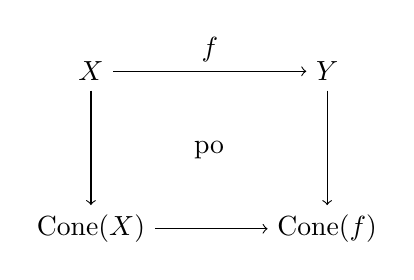
\begin{tikzpicture}
                \node (X) at (0, 0) {$X$};
                \node (Y) at (3, 0) {$Y$};
                \node (coneX) at (0, -2) {$\mathrm{Cone}(X)$};
                \node (conef) at (3, -2) {$\mathrm{Cone}(f)$};
                \node at (1.5, -1) {po};
                \draw[->] (X) -- node[above]{$f$} (Y);
                \draw[->] (X) -- (coneX);
                \draw[->] (Y) -- (conef);
                \draw[->] (coneX) -- (conef);
            \end{tikzpicture}
        \end{gather*}
    \end{remark}

\subsection{\difficult{Rational homotopy theory}}

    For the theory on differential graded algebras, see \cref{chapter:hda}.

    \newdef{Rational space}{\index{rational!space}
        A simply-connected topological space $X$ for which the homotopy groups $\pi_n(X)$ are rational vector spaces.
    }

    \newdef{Rational homotopy equivalence}{\index{rational!homotopy equivalence}
        A continuous function $f:X\rightarrow Y$ for which the induced maps on rational homotopy groups
        \begin{gather}
            \pi_n(f)\otimes\mathbb{Q}:\pi_n(X)\otimes\mathbb{Q}\rightarrow\pi_n(Y)\otimes\mathbb{Q}
        \end{gather}
        are isomorphisms for all $n\in\mathbb{N}$. An equivalent requirement is that the induced map on rational (co)homology is an isomorphism (see the section on singular homology below).
    }

    \newdef{Rational homotopy category}{
        Consider the category \textbf{Top} of topological spaces. The rational homotopy category is obtained as the \textit{localization} (see \cref{model:localization}) of \textbf{Top} with respect to the collection of rational homotopy equivalences.
    }

    \newdef{Polynomial differential forms}{
        Consider the standard $n$-simplex $\Delta^n$ (\cref{topology:simplex}). On this topological space, one can define differential forms analogous to those from \cref{section:forms}. Let $\{t_i\}_{0\leq i\leq n}$ be $n+1$ generators in degree 0 (the barycentric coordinates). Together with $n+1$ associated generators $\dr t_i$ in degree 1, one can construct the free GCA over $\mathbb{Q}$. To preserve the geometric structure of $\Delta^n$, one has to quotient out the following relations:
        \begin{gather}
            \sum_{i=0}^nt_i = 1 \qquad\text{and}\qquad \sum_{i=0}^n\dr t_i = 0\,.
        \end{gather}
        The resulting graded algebra is denoted by $\Omega^\bullet_{\text{poly}}(\Delta^n)$. In degree 0, this complex can be identified with the space of polynomial functions on $\Delta^n$. The ordinary differential forms can be obtained by taking the tensor product of $\Omega^\bullet_{\text{poly}}$ with the space of smooth functions on $\Delta^n$. Under this isomorphism, the generators $\dr t_i$ are identified with the de Rham differentials of the barycentric coordinates.

        Morphisms $f:[m]\rightarrow[n]$ in the \textit{simplex category} $\simplex$ (\cref{model:simplex_category}) induce morphisms of simplices and these in turn induce morphisms $F:\Omega^\bullet_{\text{poly}}(\Delta^n)\rightarrow\Omega^\bullet_{\text{poly}}(\Delta^m)$ defined by the following action on generators:
        \begin{gather}
            F(t_i) := \sum_{f(j)=i}t_j\,.
        \end{gather}
        It can be seen that this turns the above construction into a functor $\Omega^\bullet_{\text{poly}}:\simplex^{op}\rightarrow\mathbf{dgcAlg}$. By passing to the opposite functor and taking a left Kan extension along the Yoneda embedding $\simplex\hookrightarrow\mathbf{sSet}$, one obtains a functor $\func{\Omega^\bullet_{\text{poly}}}{sSet}{dgcAlg^{op}}$. Composition with the singular set functor $\func{\mathrm{Sing}}{Top}{sSet}$ gives the \textbf{piecewise-polynomial differential forms} functor~$\Omega^\bullet_{\text{pwpoly}}$.
    }

    \newdef{Relative Sullivan algebra}{\index{Sullivan!algebra}\label{topology:sullivan_algebra}
        An inclusion of DGCAs of the form \[(A,\dr)\hookrightarrow(A\otimes\Lambda^\bullet V,\dr')\,,\] where $V$ is a $\mathbb{N}_0$-graded vector space such that:
        \begin{itemize}
            \item there is a well-ordered set $I$ indexing a linear basis $\{e_i\}_{i\in I}$ of $V$.
            \item for all $k\in I$ and all $e_k$, one has that
            \begin{gather}
                \dr'e_k\in A\otimes\Lambda^\bullet V_{<k}\,,
            \end{gather}
            where $V_{<k}:=\mathrm{span}\{e_i\}_{i<k}$.
        \end{itemize}
        If, in addition, the implication
        \begin{gather}
            i<j\implies\deg(e_i)\leq\deg(e_j)
        \end{gather}
        holds for all $i,j\in I$, the relative Sullivan algebra is said to be \textbf{minimal}. If the Sullivan algebra is defined relative to the tensor unit $(k,0)$, where $k$ is the underlying field, it is just called a \textbf{Sullivan algebra}.
    }
    \begin{remark}
        The minimality condition admits an (equivalent) reformulation:
        \begin{gather}
            \dr V\subseteq A_{\geq1}\otimes\Lambda^\bullet V + A\otimes\Lambda^{\geq2}V\,.
        \end{gather}
    \end{remark}

    \begin{example}\label{topology:sullivan_algebras_specific}
        The free DGCA $\Lambda^\bullet V$ on a graded vector space $V$ of finite type with $V_0=V_1=0$ is a Sullivan algebra.
    \end{example}

    \newdef{Sullivan model}{\index{Sullivan!model}
        Let $X$ be a simply-connected topological space. A (minimal) Sullivan model for $X$ is a (minimal) Sullivan algebra equipped with a quasi-isomorphism to the DGA of piecewise-polynomial differential forms on $X$.
    }
    \begin{property}
        Minimal Sullivan models are unique up to isomorphism.
    \end{property}

    \begin{property}
        If $(\Lambda^\bullet V^*,\dr)$ is a minimal Sullivan model of a rational space $X$, then
        \begin{gather}
            \pi_\bullet(X)\cong V.
        \end{gather}
    \end{property}

    There is also another approach due to \textit{Quillen}. Instead of working with differential graded algebras, \textit{Quillen} used differential graded Lie algebras, i.e.~\textit{strict $L_\infty$-algebras} (see \cref{section:higher_lie_structures}).
    \begin{construct}[Sketch, Quillen]
        To every simply-connected topological space $X$, one can associate a differential graded Lie algebra $L_\bullet(X)$ such that the homology of this complex is isomorphic to the (shifted) rational homotopy complex $\pi_{\bullet+1}(X)\otimes\mathbb{Q}$ of $X$.
    \end{construct}

\subsection{\difficult{Equivariant homotopy theory}}

    In this section, topological spaces equipped with an action of a topological group $G$ will be considered (the group will often be a compact Lie group). Some notions will be defined very similarly to those in the previous section, but some others will look very differently.

    \newnot{Fixed-point space}{\index{fixed point}
        Consider a topological $G$-space $X$. The set of all its fixed points is denoted by $X^G$.
    }

    \newdef{Equivariant homotopy equivalence}{\index{homotopy!equivalence}
        A continuous function that is both an equivariant function and a homotopy equivalence in the ordinary sense.
    }
    \newdef{Weak equivariant homotopy equivalence}{
        An equivariant continuous function that restricts to an ordinary weak equivalence between the fixed-point subspaces for all closed subgroups $H\subset G$.
    }

    \begin{theorem}[Whitehead\footnotemark]\index{Whitehead}\index{Bredon}
        \footnotetext{This equivariant version of \cref{topology:whitehead} is due to \textit{Bredon}.}
        A continuous function between $G$-CW complexes is a weak equivariant homotopy equivalence if and only if it is a equivariant homotopy equivalence.
    \end{theorem}

    \newdef{Orbit category}{
        Let $G$ be a topological group. The orbit category $\mathbf{Orb}_G$ is the category defined by the following data:
        \begin{enumerate}
            \item the coset spaces $G/H$ with $H\subset G$ a closed subgroup as objects, and
            \item the equivariant homomorphisms as morphisms.
        \end{enumerate}
    }
    \begin{theorem}[Elmendorf]\index{Elmendorf}\index{orbit!category}
        The map $(X,H)\mapsto X^H$ sending a $G$-space to its fixed-point spaces can be interpreted as a functor $X:\mathbf{Orb}_G^{op}\rightarrow\mathbf{Top}$ or, equivalently, as a $\mathbf{Top}$-valued presheaf on the orbit category. By taking this a step further, one obtains a functor sending every topological space $X$ to such a presheaf.\footnote{This is the restriction of the Yoneda embedding to the subcategory $\mathbf{Orb}_G$ of $G\mathbf{Top}$.} To study the homotopy theory on these categories, one needs a choice of weak equivalences. Similar to the model structure on $\mathbf{sSet}$, one can choose the weak equivalences on $\mathbf{Psh}(\mathbf{Orb}_G)$ to be the levelwise weak equivalences. This gives an $(\infty,1)$-equivalence
        \begin{gather}
            \mathbf{Ho}(G\mathbf{Top})\cong\mathbf{Psh}(\mathbf{Orb}_G)\,.
        \end{gather}
    \end{theorem}

    \todo{COMPLETE}

\section{Simplicial homology}\label{section:homology}
\subsection{Simplices}

    \newdef{Simplex}{\index{simplex}\index{vertex}\label{topology:simplex}
        A $k$-simplex $\sigma^k\equiv[t_0,\ldots,t_k]$ is defined as the following set:
        \begin{gather}
            \sigma^k := \left\{\sum_{i=0}^k\lambda_it_i\,\middle\vert\,\sum_{i=0}^k\lambda_i = 1\text{ and }\lambda_i\geq0\right\}\,.
        \end{gather}
        where the \textbf{vertices} $t_i\in\mathbb{R}^n$ are \textbf{affinely independent}, i.e.~the vectors $t_i-t_0$ are linearly independent. Equivalently, a simplicial $k$-simplex  is the convex hull of the $k+1$ vertices $\{t_0,\ldots,t_k\}$.
    }
    \begin{remark}[Barycentric coordinates]\index{barycenter}
        The numbers $\lambda_i$ from the previous definition are called barycentric coordinates. This terminology stems from the fact that the point $\sum_{i=0}^k\lambda_it_i$ represents the \textit{barycenter} of a gravitational system consisting of masses $\lambda_i$ placed at the points $t_i$.
    \end{remark}
    \begin{example}[Standard simplex]\index{simplex!standard}\index{probability!simplex}\label{topology:standard_simplex}
        \begin{gather}
            \Delta^k := \left\{(x_0,\ldots,x_k)\in\mathbb{R}^{k+1}\,\middle\vert\,\sum_ix_i = 1 \text{ and }x_i\geq0\right\}\,.
        \end{gather}
        This simplex is also called the \textbf{probability simplex} or, sometimes, the \textbf{unit simplex}.
    \end{example}

    \newnot{Face}{\index{face}
        Consider a $k$-simplex $[v_0,\ldots,v_k]$. The \textbf{face} opposite to the vertex $v_i$ is the $(k-1)$-simplex $[v_0,\ldots,\widehat{v}_i,\ldots,v_k]$ obtained by removing the vertex $v_i$.
    }

    \newdef{Simplicial complex}{\index{simplicial!complex}
        A simplicial complex $\mathcal{K}$ is a set of simplices satisfying the following conditions:
        \begin{itemize}
            \item If $\sigma$ is a simplex in $\mathcal{K}$, so are its faces.
            \item If $\sigma_1,\sigma_2\in\mathcal{K}$, either $\sigma_1\cap\sigma_2 = \emptyset$ or $\sigma_1\cap\sigma_2$ is a face of both $\sigma_1$ and $\sigma_2$.
        \end{itemize}
        A simplicial $k$-complex is a simplicial complex where every simplex has dimension at most $k\in\mathbb{N}$.
    }

    \newdef{Path-connected complex}{\index{path!connected}
        A simplicial complex in which every two vertices are connected by an edge.
    }

    \newdef{Polyhedron}{\index{poly-!hedron}
        Consider a simplicial complex. The polyhedron associated with it is the topological space constructed by equipping the complex with the Euclidean subspace topology.
    }

    \newdef{Triangulable spaces}{\index{triangulation}\label{homalg:triangulation}
        Let $X$ be a topological space and let $\mathcal{K}$ be a polyhedron. If there exists a homeomorphism $\varphi:\mathcal{K}\rightarrow X$, then $X$ is said to be triangulable and $\mathcal{K}$ is called a \textbf{triangulation} of $X$.
    }
    \begin{property}[Fundamental group]\index{fundamental!group}
        Let $\mathcal{K}$ be a path-connected polyhedron with basepoint $a_0$ and consider a contractible one-dimensional subpolyhedron $\mathcal{C}\subset\mathcal{K}$ containing all vertices of $\mathcal{K}$. Let $G$ be the free group (\cref{group:free_group}) with generators $g_{ij}$ corresponding to the ordered 1-simplices $[v_i,v_j]\in\mathcal{K}$. On this group, one can define the following relations:
        \begin{itemize}
            \item $g_{ij} = e$ if $[v_i,v_j]\in\mathcal{C}$.
            \item $g_{ij}g_{jk} = g_{ik}$ for every ordered 2-simplex $[v_i,v_j,v_k]\in\mathcal{K}\backslash\mathcal{C}$.
        \end{itemize}
        The quotient group of $G$ by these relations is isomorphic to the fundamental group $\pi_1(\mathcal{K},a_0)$.
    \end{property}
    \begin{result}
        \Cref{topology:homeomorphic_homotopy}, which states that homeomorphic spaces have the same homotopy groups, implies that the fundamental group of a triangulable space can be computed by looking at any of its triangulations.
    \end{result}

\subsection{Simplicial homology}\index{homology!simplicial}

    In this section, a chain complex (\cref{homalg:chain_complex}) and its associated homology theory are constructed for triangulable spaces.

    \newdef{Chain group}{\label{topology:chain_group}
        Let $\mathcal{K}$ be a simplicial $n$-complex. The $k^{\text{th}}$ chain group $C_k(\mathcal{K})$ is defined as the free Abelian group generated by the $k$-simplices in $\mathcal{K}$:
        \begin{gather}
            C_k(\mathcal{K}) := \left\{\sum_ia_i\sigma_i\,\middle\vert\,\sigma_i\text{ is a $k$-simplex in $\mathcal{K}$}, a_i\in\mathbb{Z}\right\}\,.
        \end{gather}
        For $k>n$ and $k<0$, $C_k(\mathcal{K})$ is defined to be $\{0\}$.
    }

    \newdef{Boundary operator}{
        The boundary operator $\partial_k:C_k(\mathcal{K})\rightarrow C_{k-1}(\mathcal{K})$ is the group morphism defined by the following properties:
        \begin{itemize}
            \item\textbf{Linearity}:
                \begin{gather}
                    \partial_k\Bigl(\sum_ia_i\sigma_i\Bigr) = \sum_ia_i\partial_k\sigma_i\,,
                \end{gather}
            \item\textbf{Action on generators}
                \begin{gather}
                    \begin{aligned}
                        \partial_k[v_0,\ldots,v_k] &= \sum_{i=0}^k(-1)^i[v_0,\ldots,\hat{v}_i,\ldots,v_k]\,,\\
                        \partial_0[v] &= 0\,.
                    \end{aligned}
                \end{gather}
        \end{itemize}
    }

    \begin{property}[Chain condition]\label{topology:boundary_operator_relation}
        The boundary operators satisfy the following relation:
        \begin{gather}
            \partial_k\circ\partial_{k+1} = 0\,.
        \end{gather}
        This property turns the system $(C_k,\partial_k)$ into a chain complex (\cref{homalg:chain_complex}).
    \end{property}

    \newdef{Cycle group}{
        The $k^{\text{th}}$ cycle group $Z_k(\mathcal{K})$ is defined as the set of $k$-chains $\sigma_k$ such that $\partial_k\sigma_k = 0$. These chains are called \textbf{cycles}.
    }
    \newdef{Boundary group}{
        The $k^{\text{th}}$ boundary group $B_k(\mathcal{K})$ is defined as the set of $k$-chains $\sigma_k$ for which there exists a $(k+1)$-chain $b$ such that $\partial_{k+1}b = \sigma_k$. These chains are called \textbf{boundaries}.
    }
    \newdef{Homology group}{\label{topology:simplicial_homology_group}
        From \cref{topology:boundary_operator_relation}, it follows that $B_k(\mathcal{K})\subset Z_k(\mathcal{K})$ is a subgroup (it is a normal subgroup because of the Abelian character). One can thus define the $k^{\text{th}}$ homology group $H_k(\mathcal{K})$ as the following quotient group:
        \begin{gather}
            H_k(\mathcal{K}) := Z_k(\mathcal{K})/B_k(\mathcal{K})\,.
        \end{gather}
        \Cref{group:theorem:free_group} says that $H_k(\mathcal{K})$ can be written as $G_k\oplus T_k$. Both of these groups say something about $\mathcal{K}$. The rank of $G_k$, denoted by $R_k(\mathcal{K})$, is equal to the number of $(k+1)$-dimensional holes in $\mathcal{K}$. The torsion subgroup $T_k$ says how the space $\mathcal{K}$ is `twisted'.
    }

    \newdef{Betti numbers}{\index{Betti number}
        The ranks $R_k(\mathcal{K})$ are called the Betti numbers of $\mathcal{K}$.
    }
    \begin{definition}[Euler characteristic]\index{Euler!characteristic}\index{Euler--Poincar\'e formula}\label{topology:euler_characteristic}
        The Euler characteristic of a triangulable space $X$ is defined as follows:
        \begin{gather}
            \chi(X) := \sum_i(-1)^iR_i(X)\,.
        \end{gather}
        This formula is sometimes called the \textbf{Poincar\'e} or \textbf{Euler--Poincar\'e formula}.
    \end{definition}

    \begin{property}[Isomorphisms]
        If two topological spaces have the same homotopy type, in particular when they are homeomorphic, they have isomorphic homology groups.
    \end{property}
    \begin{result}
        As was the case for the fundamental group, it follows from the definition of a triangulation that one can study the homology groups of a given triangulable space by looking at any of its triangulations.
    \end{result}

    Although the homology invariants do not depend on the choice of triangulation, a remark about the existence of nonequivalent triangulations should be given.
    \begin{remark}[Hauptvermutung]\index{Hauptvermutung}
        Before the construction of a counterexample, it was believed (hence the terms \textit{Hauptvermutung} in German or \textit{main conjecture} in English) that every two triangulations of a topological space allowed a common refinement and, hence, where equivalent for many constructions. However, it was shown that this conjecture is generally false, e.g.~for topological manifolds in dimensions 5 and higher, there exist an infinite number of nonequivalent triangulations. In dimensions up to 4, it was proven by Rad\'o and Moise that the Hauptvermutung holds for all topological manifolds (see also \cref{manifold:rado_moise}).
    \end{remark}

    \begin{construct}
        The definition of homology groups can be generalized by letting the (formal) linear combinations used in the definition of the chain group be of the following form:
        \begin{gather}
            c = \sum_ig_i\sigma_i^k\,,
        \end{gather}
        where $g_i\in G$ for some Abelian group $G$. The $k^{\text{th}}$ homology group of $X$ with coefficients in $G$ is denoted by $H_k(X;G)$.
    \end{construct}
    \begin{property}[Vanishing torsion]
        When $G$ is a field, such as $\mathbb{Q}$ or $\mathbb{R}$, the torsion subgroups $T_k$ vanish. The relation between integral homology and homology with coefficients in a group is given by the \textit{universal coefficient theorem}.
    \end{property}

    \newformula{K\"unneth formula}{\index{K\"unneth formula}
        Let $X,Y$ be two simplicial complexes. The homology groups of the Cartesian product $X\times Y$ with coefficients in a field $\mathfrak{K}$ is given by
        \begin{gather}
            H_k(X\times Y;\mathfrak{K}) = \bigoplus_{k=i+j}H_i(X;\mathfrak{K})\otimes H_j(Y;\mathfrak{K})\,.
        \end{gather}
        When the requirement of $\mathfrak{K}$ being a field is relaxed to it merely being a group, the torsion subgroups have to be taken into account. See the literature for this general form.
    }

\subsection{Relative homology}\index{homology!relative}

    In this section, the homology of a simplicial complex $\mathcal{K}$ `modulo' a subcomplex $\mathcal{L}$ is considered.

    \newdef{Relative chain group}{
        The $k$-chain group of $\mathcal{K}$ modulo $\mathcal{L}$ is defined as the following quotient group:
        \begin{gather}
            C_k(\mathcal{K},\mathcal{L}) := C_k(\mathcal{K})/C_k(\mathcal{L})\,.
        \end{gather}
        Equivalence classes will be denoted by square brackets $[c]$, where $c\in C_\bullet(\mathcal{K})$.
    }
    \newdef{Relative boundary operator}{
        The relative boundary operator $\overline\partial_k$ is defined as follows:
        \begin{gather}
            \overline\partial_k[c_k] := [\partial_kc_k]\,,
        \end{gather}
        where $\partial_k$ on the right-hand side denotes the boundary operator in ordinary homology. This is a well-defined operation since $\partial C_\bullet(\mathcal{L})\subseteq C_\bullet(\mathcal{L})$.
    }
    \newdef{Relative homology groups}{
        The relative cycle and relative boundary groups are defined analogous to their ordinary counterparts. The relative homology groups are defined as follows:
        \begin{gather}
            H_k(\mathcal{K},\mathcal{L}) := \frac{\ker(\overline\partial_k)}{\im(\overline\partial_{k+1})}\,.
        \end{gather}
        Elements $h_k\in H_k(\mathcal{K},\mathcal{L})$ can be represented as $h_k=z_k + C_k(\mathcal{L})$ such that $\partial_kz_k\in C_{k-1}(\mathcal{L})$.
    }

    \begin{property}[Homotopy invariance]
        Consider two (triangulable) topological spaces $X,Y$ with subspaces $A\subset X,B\subset Y$. If a continuous function $f:X\rightarrow Y$ is a homotopy equivalence such that the restriction to $A$ gives a homotopy equivalence $f|_A:A\rightarrow B$, the relative homology complexes $H_\bullet(X,A)$ and $H_\bullet(Y,B)$ are isomorphic.
    \end{property}

    \begin{property}[Long sequence for a pair]
        The relative homology groups fit in the following (long) exact sequence:
        \begin{gather}
            \cdots\longrightarrow H_k(\mathcal{L})\overset{i_\ast}{\longrightarrow}H_k(\mathcal{K})\overset{j_\ast}{\longrightarrow}H_k(\mathcal{K},\mathcal{L})\overset{\partial_k}{\longrightarrow}H_{k-1}(\mathcal{L})\longrightarrow\cdots\,,
        \end{gather}
        where $i_\ast$ and $j_\ast$ are the homology morphisms induced by the inclusions $i:\mathcal{L}\rightarrow \mathcal{K}$ and $j:\mathcal{K}\rightarrow(\mathcal{K},\mathcal{L})$.
    \end{property}

    \begin{theorem}[Excision theorem]\index{excision}\label{topology:excision_theorem}
        Let $U,V$ and $X$ be simplicial complexes such that $U\subset V\subset X$. If the closure $\overline{U}$ is contained in the interior $V^\circ$, then
        \begin{gather}
            H_k(X,V) \cong H_k(X\backslash U,V\backslash U)\,.
        \end{gather}
    \end{theorem}

    \newdef{Reduced homology}{\index{homology!reduced}
        Consider the chain complex $C_\bullet(X)$. \Cref{topology:point_homology} says that a point $\{\ast\}$ has homology $\mathbb{Z}$ concentrated in degree $0$. However, it would be nice if $\{\ast\}$ had vanishing homology. To this end, one can augment (\cref{homalg:resolution}) the chain complex $C_\bullet(X)$ of any topological space by the group $\mathbb{Z}$ to obtain the reduced homology complex $\widetilde{H}_\bullet(X)$:
        \begin{gather}
            H_k(X) \cong
            \begin{cases}
                \widetilde{H}_0(X)\oplus\mathbb{Z}&\cif k=0\,,\\
                \widetilde{H}_k(X)&\cif k\neq0\,.
            \end{cases}
        \end{gather}
    }
    \begin{property}
        Consider a pointed topological space $(X,x_0)$. The reduced homology $\widetilde{H}_\bullet(X)$ is isomorphic to the relative homology $H_\bullet(X,\{x_0\})$.
    \end{property}

    \begin{property}[Good pair]\index{neighbourhood!deformation retract}\label{topology:ndr_pair_homology}
        Consider a topological space $X$ together with a subspace $A$. The pair $(X,A)$ is called a \textbf{neighbourhood deformation retract (NDR) pair}\footnote{Some authords call this a \textbf{good pair}, while others define an NDR pair more restrictively.} if there exists a neighbourhood $V\subset X$ of $A$ such that $V$ deformation retracts onto $A$. Equivalently, the inclusion $A\subset X$ is a closed cofibration (\cref{topology:cofibration}).

        Given an NDR pair $(X,A)$, there exists an isomorphism
        \begin{gather}
            H_\bullet(X,A)\cong\widetilde{H}_\bullet(X/A)\,.
        \end{gather}
    \end{property}

    \todo{STREAMLINE TERMINOLOGY AND NOTATION (topological space vs. triangulable space vs. simplicial complex, X vs K, ...)}

\subsection{Examples}

    \begin{example}\label{topology:point_homology}
        Let $X$ be a contractible space.
        \begin{gather}
            H_k(X) =
            \begin{cases}
                \mathbb{Z}&\cif k=0\\
                0&\text{otherwise}
            \end{cases}
        \end{gather}
    \end{example}
    \begin{example}
        Let $\mathcal{K}$ be a path-connected simplicial complex.
        \begin{gather}
            H_0(\mathcal{K}) = \mathbb{Z}
        \end{gather}
        Furthermore, every point $p\in\mathcal{K}$ determines a generator $\langle p \rangle\in H_0(\mathcal{K})$.
    \end{example}

    \begin{example}
        The homology groups of the $n$-sphere $S^n$ are given by
        \begin{gather}
            H_k(S^n)=
            \begin{cases}
                \mathbb{Z}&\cif k=0\text{ or }k=n\,,\\
                0&\text{otherwise}\,.
            \end{cases}
        \end{gather}
    \end{example}

    \newdef{Homology sphere}{\index{homology!sphere}
        An \textit{$n$-dimensional manifold} (see \cref{chapter:manifolds}) having the same homology groups as the $n$-sphere.
    }
    \newdef{Degree}{\index{degree!of map}\label{topology:degree}
        The example above says that $H_n(S^n)=\mathbb{Z}$ for any $n\in\mathbb{N}$. Given a map $f:S^n\rightarrow S^n$, the induced map $f_*$ on homology is an endomorphism of $\mathbb{Z}$ and, hence, is of the form $f(x)=\lambda x$ where $\lambda \in\mathbb{Z}$. The coefficient $\lambda$ is called the degree of $f$, sometimes denoted by $\deg(f)$.
    }
    \begin{property}
        Two maps $f:S^n\rightarrow S^n$ have the same degree if and only if they are homotopic.
    \end{property}

    \begin{example}
        Consider the closed (or open) disks $D_n$.
        \begin{gather}
            H_k(D_n,\partial D_n) =
            \begin{cases}
                \mathbb{Z}&\cif k=n\\
                0&\text{otherwise}
            \end{cases}
        \end{gather}
        This holds for any $n$-skeleton $X^n$ of a CW-complex.
    \end{example}

\section{Singular homology}\label{section:singular_homology}

    \newdef{Singular simplex}{\index{simplex!singular}
        Recall the $k$-simplex $\Delta^k$ from \cref{topology:standard_simplex}. A singular $k$-simplex in a topological space $X$ is defined as a continuous function $\sigma:\Delta^k\rightarrow X$.
    }
    \sremark{The name singular comes from the fact that the function $\sigma$ need not be injective.}

    \newdef{$\Delta$-complex}{\index{$\Delta$-complex}\index{cellular complex}
        Let $\{\sigma_i:\Delta^n\rightarrow X\}_{i\in I}$ be a collection of singular simplices in $X$, where the dimension $n\in\mathbb{N}$ may depend on the index $i\in I$. This collection forms a $\Delta$-complex on $X$ if it satisfies the following conditions:
        \begin{itemize}
            \item The restrictions $\sigma_i|_{\overset{\circ}{\Delta}{}^n}$ are injective and every point in $X$ lies in the image of exactly one such restriction.
            \item The restriction of a simplex $\sigma_i$ to any one of the faces of $\Delta^n$ is equal to some other $\sigma_j$.
            \item A subset $Y\subseteq X$ is open if and only if all of its inverse images $\sigma_i^{-1}(Y)$ are open.
        \end{itemize}

        Similar to a CW-complex or \textit{cellular complex}, these conditions imply that every $\Delta$-complex can be constructed inductively from a (discrete) set of vertices by gluing and identifying edges.
    }

    \newdef{Singular chain group}{\index{chain}
        The singular chain group $S_k(X)$ with coefficients in a group $G$ is defined as the set of formal linear combinations $\sum_ig_i\sigma_i$, where the $\sigma_i$ are singular $k$-simplices in $X$. The basis of this free group is, in most cases, infinite as there are, in general, many ways to map $\Delta^k$ to $X$.
    }

    Before continuing, one first need to introduce an important concept in the context of simplicial objects.
    \newdef{Face map}{\index{face!map}
        The face maps are morphisms $\varepsilon_i^k:\Delta^{k-1}\rightarrow\Delta^k$ that map $\Delta^{k-1}$ onto the $i^{\text{th}}$ face of $\Delta^k$. They are explicitly given by
        \begin{gather}
            \varepsilon_i^k(s_0,\ldots,s_{k-1}) := (s_0,\ldots,s_{i-1},0,s_i,\ldots,s_{k-1})\,.
        \end{gather}
        Their defining property is the following relation:
        \begin{gather}
            \varepsilon_i^k\circ\varepsilon_j^{k-1} = \varepsilon_j^k\circ\varepsilon_{i-1}^{k-1}\,,
        \end{gather}
        where $j\leq i$.
    }
    \sremark{Some authors (for example the authors at \textit{nLab}) call these maps \textit{degeneracy maps} and call what in these notes are called \textit{degeneracy maps}, face maps. This is a consequence of working in the dual picture (they work in the opposite of the \textit{simplex category} $\simplex$).}

    \newdef{Singular boundary operator}{\index{face!map}
        The singular boundary operator\footnote{The same notation as for simplicial boundary operators is used for simplicity.} $\partial$ is defined by its linear action on the singular chain groups $S_k(X;G)$. It follows, that it is uniquely defined by its action on the singular $k$-simplices $\sigma^k$.

        The action of the boundary operator on the singular $k$-simplex $\sigma^k$ is given by
        \begin{gather}
            \partial_k\sigma^k = \sum_{i=0}^k(-1)^i\sigma^k\circ\varepsilon^k_i\,,
        \end{gather}
        where the $\varepsilon^k_i$ are the face maps defined above. The singular boundary operators satisfy the same relation as the the simplicial boundary operators:
        \begin{gather}
            \partial_{k-1}\circ\partial_k = 0\,.
        \end{gather}
        It follows, that $S_k(X;G)$ is also a chain complex.
    }

    \newdef{Singular homology group}{\index{homology!singular}
        The singular homology groups of a topological space with coefficients in an Abelian group $G$ are defined as follows:
        \begin{gather}
            H_k(X;G) := \frac{\ker(\partial_k)}{\im(\partial_{k+1})}\,.
        \end{gather}
    }
    \begin{property}[Simplicial homology]
        For triangulable spaces, singular homology is isomorphic to simplicial homology. When a space is not triangulable, this property is not valid. The singular approach to homology is more general, but it is often more difficult to compute (even in the case of triangulable spaces).
    \end{property}

    \begin{property}[Induced morphism]\index{pushforward!of homology}\label{topology:pushforward}
        Consider a continuous function $f:X\rightarrow Y$ between topological spaces. This induces a morphism $f_*:S_k(X;G)\rightarrow S_k(Y;G)$ on the chain groups as follows:
        \begin{gather}
            f_*\Bigl(\sum_\sigma c_\sigma\sigma\Bigr) := \sum_\sigma c_\sigma f\circ\sigma\,.
        \end{gather}
        This map takes cycle (resp.~boundary) groups to (subgroups of) cycle (resp.~boundary) groups and, hence, induces a morphism of homology groups, called the \textbf{pushforward}:
        \begin{gather}
            f_\ast:H_k(X)\rightarrow H_k(Y):\langle h \rangle\mapsto\langle f_*(h)\rangle\,.
        \end{gather}
    \end{property}
    \begin{result}
        $H_k$ is a functor $\mathbf{Top}\rightarrow\mathbf{Ab}$ that maps topological spaces to their homology groups and continuous functions $f$ to their pushforwards $f_\ast$.
    \end{result}

    \begin{theorem}[Hurewicz]\index{Hurewicz}
        Let $X$ be path connected and let $[\cdot]$ and $\langle\cdot\rangle$ denote the equivalence classes in the homotopy and homology groups, respectively. Because every path can be obtained as a singular one-chain, the map $\pi_1(X)\rightarrow H_1(X):[\gamma]\mapsto\langle\gamma\rangle$ defines a group morphism. Furthermore, this map induces an isomorphism 
        \begin{gather}
            \pi_1(X)/[\pi_1(X),\pi_1(X)] \cong H_1(X)\,.
        \end{gather}
        More generally, for every topological space $X$ and every $k\in\mathbb{N}$, there exists a morphism $h_*:\pi_k(X)\rightarrow H_k(X)$. If $Y$ is $(n-1)$-connected, then, for every $k\leq n$, this morphism is in fact an isomorphism.
    \end{theorem}

    \newdef{Singular cohomology}{\index{cohomology!singular}\index{pullback!of cohomology}
        The singular cohomology groups of a topological space $X$ with coefficients in an Abelian group $G$ are defined as follows:\footnote{Actually this is the \textit{Universal Coefficient Theorem} when defining cohomology through a suitable hom-complex.}
        \begin{gather}
            H^k(X;G) := \hom\bigl(H_k(X),G\bigr)\,,
        \end{gather}
        where, on the right-hand side, the integral (singular) homology of $X$ is used. A continuous function $f:X\rightarrow Y$ induces a \textbf{pullback} morphism $f^*:H^\bullet(Y;G)\rightarrow H^\bullet(X;G)$ on cohomology by duality:
        \begin{gather}
            f^*g(\sigma) := g(f_*\sigma)\,,
        \end{gather}
        where $f_*$ is the pushforward (\cref{topology:pushforward}) induced by $f$.
    }
    \begin{property}[Representability]
        Let $X$ be a CW complex. There exists an isomorphism
        \begin{gather}
            [X,K(G,n)]\rightarrow H^n(X;G)
        \end{gather}
        between the homotopy classes of maps $X\rightarrow K(G,n)$ and the $n^{\text{th}}$ singular cohomology of $X$ with coefficients in $G$. (This result can be widely generalized cf.~\cref{topology:brown} further below.)
        \begin{mdframed}[roundcorner=10pt, linecolor=blue, linewidth=1pt]
            \begin{proof}
                Consider the Eilenberg--Maclane space $K(G,n)$ for $G$ (\cref{topology:eilenberg_maclane}). By the Hurewicz theorem, there exists an isomorphism $H_n\bigl(K(G,n)\bigr)\cong\pi_n\bigl(K(G,n)\bigr)\cong G$. By definition of cohomology, $H^n\bigl(K(G,n);G\bigr)=\hom\bigl(H_n(K(G,n)),G\bigr)$ and, thus, $H^n\bigl(K(G,n);G\bigr)\cong\hom(G,G)$. In particular, there corresponds a cohomology class $\psi$ to the identity mapping on $G$. The cohomology class in $H^n(X;G)$ associated to a homotopy class of functions $f:X\rightarrow K(G,n)$ is given by $f^*\psi$.
            \end{proof}
        \end{mdframed}
    \end{property}

\section{Local coefficients}\index{local!coefficients}\label{section:local_coefficients}

    For some applications, one needs to generalize the notion of (co)homology. For example, when considering integration theory on \textit{manifolds} (see \cref{section:compact_cohomology}), one needs to take into account the nonorientability.

    Consider a topological space $X$ that admits a universal cover $\widetilde{X}$. By \cref{topology:universal_cover_automorphisms}, one then has
    \begin{gather}
        X\cong\widetilde{X}/\pi_1(X)\,.
    \end{gather}
    Given a $\mathbb{Z}[\pi_1(X)]$-module $A$, one defines the $A$-twisted chain (singular) group of $X$ as
    \begin{gather}
        C(X;A):=C(\widetilde{X})\otimes_{\mathbb{Z}[\pi_1(X)]}A\,.
    \end{gather}
    The automorphism group $\pi_1(X)$ of $\widetilde{X}$ acts on singular simplices by postcomposition.

    When $A$ is a trivial $\pi_1(X)$-module, the tensor product structure enforces that the orbit of every automorphism collapses and, hence, $C(\widetilde{X})\otimes_{\mathbb{Z}[\pi_1(X)]}A\cong C(X)\otimes_{\mathbb{Z}}A$. It follows, that the ordinary singular cohomology with coefficients in $A$ is recovered (as expected).

    \todo{COMPLETE}

\section{\difficult{Axiomatic approach}}\label{section:eilenberg_steenrod}

    \newdef{Eilenberg--Steenrod axioms}{\index{Eilenberg--Steenrod axioms}\label{topology:eilenberg_steenrod_axioms}
        All (co)homology theories have a set of properties in common. By treating these properties as axioms, one can construct relative (co)homology theories as a sequence of functors $H_k:\mathbf{Top}\times\mathbf{Top}\rightarrow\mathbf{Ab}$.\footnote{Technically, one should replace $\mathbf{Top}\times\mathbf{Top}$ by the category consisting of subspace inclusions $A\hookrightarrow X$.} The axioms are as follows:
        \begin{enumerate}
            \item\textbf{Homotopy invariance}: If $f,g$ are homotopic maps, their induced homology maps are the same: \[f\cong g\implies\forall k\in\mathbb{N}:H_k(f) = H_k(g).\]
            \item\textbf{Excision}: If $U\subset V\subset X$ and $\overline U\subset V^\circ$, then $H_k(X,V)\cong H_k(X\backslash U,V\backslash U)$.
            \item\textbf{Additivity}: If $X = \bigsqcup_i X_i$, then $H_k(X)\cong\bigoplus_i H_k(X_i)$.
            \item\textbf{Exactness}: Each pair $(X,A)$, where $A\subset X$, induces a long exact sequence
            \begin{gather}
                \cdots\longrightarrow H_k(A)\overset{i_\ast}{\longrightarrow}H_k(X)\overset{j_\ast}{\longrightarrow}H_k(X,A)\overset{\partial_k}{\longrightarrow}H_{k-1}(A)\longrightarrow\cdots,
            \end{gather}
            where $i_\ast$ and $j_\ast$ are the pushforwards of the inclusions $i:A\rightarrow X$ and $j:X\rightarrow(X,A)$.
            \item\textbf{Dimension}: If $X$ is a singleton, then $H_k(X) = \{0\}$ for all $k\geq1$. The group $H_0(X)$ is called the \textbf{coefficient group} and gives the coefficients used in the linear combinations of the chain group.
        \end{enumerate}
    }
    \begin{remark}
        If the dimension axiom is removed from the set of axioms, the so-called \textit{extraordinary (or generalized) homology theories} are obtained.
    \end{remark}

    Although the following theorem sounds like more of a purely category-theoretic statement, its main application is the definition of cohomology theories.
    \begin{theorem}[Brown's representability theorem]\index{Brown's representability theorem}\index{Mayer--Vietoris}\label{topology:brown}
        Consider a presheaf $H$ on the homotopy category of pointed connected topological spaces $\mathbf{Ho}(\mathbf{Top}^{\text{con}}_*)$. This functor is representable if and only if it satisfies the following conditions:
        \begin{itemize}
            \item It maps coproducts to products.
            \item It maps weak pushouts to weak pullbacks. (Weak pushouts in the homotopy category $\mathbf{Ho}(\mathbf{Top})$ come from homotopy pushouts in $\mathbf{Top}$.)
        \end{itemize}
    \end{theorem}
    \begin{remark}
        If one constructs the homotopy category using the CW-model structure in $\mathbf{Top}$, the second condition can be restated as a \textit{Mayer--Vietoris axiom}. Consider a CW complex $U$ and two subcomplexes $V_1,V_2$. If $x\in H(V_1),y\in H(V_2)$ and $x=y$ on the intersection $V_1\cap V_2$, there exists a $z\in H(U)$ that restricts to $x$ (resp.~$y$) on $V_1$ (resp.~$V_2$).
    \end{remark}
    \begin{result}[Cohomology]
        Generalized cohomology theories are representable. Given cohomology functors $\{H^n\}_{n\in\mathbb{N}}$, there exists a sequence of pointed topological spaces $\seq{X}$ such that
        \begin{gather}
            H^n(Y) := [Y,X_n]
        \end{gather}
        for all $n\in\mathbb{N}$.
    \end{result}

    For reduced cohomology theories, there exist suspension isomorphisms
    \begin{gather}
        \widetilde{H}^n(Y)\cong\widetilde{H}^{n+1}(\Sigma Y)\,.
    \end{gather}
    Under Brown's theorem, these induce isomorphisms $X_n\cong\Omega X_{n+1}$. This endows the sequence of spaces $\seq{X}$ with the following structure.
    \newdef{Spectrum\footnotemark}{\index{spectrum}\label{topology:spectrum}
        \footnotetext{Sometimes called an $\Omega$-spectrum to distinguish it from other, possibly more general, spectra.}
        A sequence of pointed topological spaces $\seq{X}$ satisfying
        \begin{gather}
            X_n\cong\Omega X_{n+1}\,.
        \end{gather}
        (The isomorphism can be a weak homotopy equivalence or homeomorphism depending on the context.) A weaker definition, that of \textbf{prespectra} or \textbf{sequential spectra}, is that of a sequence of pointed topological spaces $\seq{X}$ with structure morphisms $\Sigma X_n\rightarrow X_{n+1}$, where $\Sigma$ is the reduced suspension functor. By Eckman--Hilton duality, every $\Omega$-spectrum is a prespectrum.

        Every prespectrum gives rise to a spectrum by taking a direct limit over loop spaces:\footnote{The notion, similar to the one in \cref{topology:loop_space}, stems from the relation to loop spaces in the case of suspensions $X_n=\Sigma^n Y$ (\cref{topology:suspension}).}
        \begin{gather}
            (LX)_n := \varinjlim_{k\in\mathbb{N}}\Omega^kX_{n+k}\,.
        \end{gather}
        This gives a \textit{fibrant replacement functor} in the \textit{model structure} on spectra.
    }
    \begin{property}
        Brown's representability theorem shows that there exists a bijection between isomorphism classes of (generalized) cohomology theories and homotopy-equivalence classes of spectra.
    \end{property}

    \begin{property}[Eilenberg--MacLane spectrum]\index{Eilenberg--MacLane!spectrum}
        The Eilenberg--MacLane spectrum of an Abelian group $A$ is the sequence of Eilenberg--MacLane spaces $\{K(A,n)\}_{n\in\mathbb{N}}$. By the \textit{Dold--Kan theorem} (see \cref{model:dold_kan}), Abelian groups form a subcategory of Abelian chain complexes: $\mathbf{Ab}\hookrightarrow\mathbf{Ch}^+(\mathbf{Ab})$. The Eilenberg--MacLane assignment extends to a functor $\mathcal{D}(\mathbf{Ab})\rightarrow\mathbf{Spectra}$ from the derived category of Abelian chain complexes to the category of ($\Omega$-)spectra.
    \end{property}

    \begin{property}
        There exists an ($\infty$-)equivalence between $\mathbf{Sp}$ and $\infty\mathbf{Grpd}$. The left adjoint sends (a topological space representing) a given homotopy type to its suspension spectrum. The right adjoint sends a spectrum $\seq{X}$ to (the homotopy type of) its infinite loop space
        \begin{gather}
            \Omega^\infty X:=X_0\cong\varinjlim_{k\in\mathbb{N}}\Omega^kX_k\,.
        \end{gather}
    \end{property}

\section{\difficult{Equivariant cohomology}}\index{equivariant!cohomology}

    In this section, the action of (topological) groups $G$ on topological spaces will be considered. These spaces will be called topological $G$-spaces or just $G$-spaces. See, for example, \citet{cartier_mad_2001,rozenblyum_bung_2023}. The content of \cref{chapter:sheaf} is used.

\subsection{Borel construction}

    \newdef{Equivariant cohomology}{\label{topology:equivariant_cohomology}
        Let $X$ be a topological $G$-space for which the $G$-action is free. The equivariant cohomology of $X$ is defined as
        \begin{gather}
            H_G^\bullet(X) := H^\bullet(X/G)\,,
        \end{gather}
        where $X/G$ is the orbit space with respect to the action of $G$ on $X$.
    }

    If the action is not free, a more general construction needs to be used. Consider the \textit{universal bundle} $\pi:EG\rightarrow BG$ from \cref{bundle:classifying_space}. From this bundle, one can construct the associated bundle $EG\times_G X$. This is sometimes called the \textbf{Borel construction}. It gives a model for the homotopy quotient $X/\!\!/G$, with $BG\cong\ast/\!\!/G$. The $G$-equivariant cohomology of $X$ is then defined as the singular cohomology of the Borel construction:\index{Borel!construction}
    \begin{gather}
        H_G^\bullet(X) := H^\bullet(EG\times_GX)\,.
    \end{gather}

    \todo{COMPLETE (E.G. LECTURES OF TU ON YOUTUBE)}

\subsection{Classifying topoi and stacks}

    The topological constructions from the previous section can reformulated in a more categorical/topos-theoretic way. As a first step, the Borel construction is rephrased.
    \begin{property}
        The geometric realization (\cref{model:geometric_realization_categories}) of the action groupoid (\cref{cat:action_groupoid}) is isomorphic to the Borel construction:
        \begin{gather}
            |X/\!\!/G|\cong EG\times_GX\,.
        \end{gather}
    \end{property}

    \newdef{Classifying topos}{\index{classifying!topos}\index{equivariant!sheaf}
        First, consider a discrete group $G$. The classifying topos $\mathcal{B}G$ is defined as the category of $G$-sets together with equivariant maps. Equivalently, consider the delooping groupoid $\mathbf{B}G$ (\cref{cat:group_delooping}). $\mathcal{B}G$ is equivalent to the (pre)sheaf topos on the classifying space $BG\cong|\mathbf{B}G|$.

        For general topological groups, the situation is more complicated. Instead of having the trivial (Grothendieck) topology on the category of $G$-sets, $G$-equivariant covers have to be considered, i.e.~topological covers consisting of equivariant maps. The classifying topos $\mathcal{B}G$ then consist of sheaves on this site, i.e.~the $G$-\textit{equivariant sheaves} (see \cref{sheaf:equivariant_sheaf}).
    }

    \newdef{Quotient stack}{\index{quotient!stack}
        Consider a topological group $G$ and a topological space $X$. The quotient stack $[X/G]$ is the stack (\cref{section:stacks}) that assigns to any topological space $Y$ the following groupoid:
        \begin{enumerate}
            \item\textbf{Objects}: Pairs $(\pi:P\rightarrow Y,f:P\rightarrow X)$, where $\pi$ is a principal $G$-bundle and $f$ is $G$-equivariant.
            \item\textbf{Morphisms}: $G$-equivariant isomorphisms.
        \end{enumerate}

        Equivalently, consider the action groupoid $X/\!\!/G$ (\cref{cat:action_groupoid}). This groupoid induces a prestack that assigns to every topological space $Y$ the action groupoid $\underline{X}(Y)/\!\!/\underline{G}(Y)$. The sheafification of this prestack is equivalent to $[X/G]$.
    }
    \begin{example}\index{classifying!stack}
        When $X$ is trivial, the delooping groupoid $\mathbf{B}G$ is recovered, which is also called the \textbf{classifying stack} in this form. On the other hand, when $G$ is trivial, the representable stack $\underline{X}$ is recovered.
    \end{example}
% \chapter{Sheaf Theory}\label{chapter:sheaf}

    A reference aimed towards the study of differential geometry is~\citet{brylinski_loop_1993}. For the concept of a sheaf in category theory, see \cref{section:grothendieck_topos}.

    \minitoc

\section{Presheaves}

    \newdef{Presheaf}{\index{presheaf}\index{section!of a (pre)sheaf}
        Let $(X,\tau)$ be a topological space. A presheaf on $X$ consists of a choice of algebraic structure $\mathcal{F}(U)$ for every open set $U\in\tau$ and a morphism $\Phi^U_V:\mathcal{F}(U)\rightarrow \mathcal{F}(V)$ for every two open sets $U,V\in\tau$ with $V\subseteq U$ such that the following conditions are satisfied:
        \begin{enumerate}
            \item $\Phi^U_U = \mathbbm{1}_{\mathcal{F}(U)}$, and
            \item $W\subseteq V\subseteq U\implies\Phi^U_W = \Phi^V_W\circ\Phi^U_V$.
        \end{enumerate}
        The set $\mathcal{F}(U)$ is called the set of \textbf{sections} over $U$ and the morphisms $\Phi^U_V$ are called the \textbf{restriction maps}.
    }
    \newdef{Morphism of presheaves}{\index{morphism!of presheaves}\index{germ}
        Let $\mathcal{F},\mathcal{F}'$ be two presheaves on a topological space $X$. A morphism $\mathcal{F}\rightarrow\mathcal{F}'$ is a set of morphisms $\Psi_U:\mathcal{F}(U)\rightarrow\mathcal{F}'(U)$ that commute with the restriction maps $\Phi^U_V$.
    }

    \begin{adefinition}[Categorical definition]
        Using the language of category theory one can give a more concise definition. Let $\mathbf{C}$ be a category and let $X$ be a topological space. A $\mathbf{C}$-valued presheaf on $X$ is a contravariant functor $\mathcal{F}:\mathbf{Open}(X)\rightarrow\mathbf{C}$. A morphism of presheaves is a natural transformation between such functors. As such the category of presheaves on a topological space $X$ is in fact the presheaf topos on $\mathbf{Open}(X)$.
    \end{adefinition}

    \begin{example}[Constant presheaf]\label{sheaf:constant_presheaf}
        Let $S$ be any set. The constant presheaf on $X$ with target $S$ is defined by
        \begin{gather}
            \mathcal{F}(U) := S
        \end{gather}
        for every open set $U\subseteq X$.
    \end{example}

\section{Sheaves}

    \newdef{Sheaf}{\index{sheaf}\label{sheaf:def}
        Let $(X,\tau)$ be a topological space. A sheaf on $X$ is a presheaf $\mathcal{F}$ satisfying the following conditions:
        \begin{enumerate}
            \item\textbf{Locality (or separation)}: Let $\{U_i\}_{i\in I}\subset\tau$ be an open cover of $U\subseteq X$ and consider sections $s,t\in\mathcal{F}(U)$. If $\forall i\in I:s|_{U_i}=t|_{U_i}$, then $s=t$. This is equivalent to saying that that $\mathcal{F}(U)$ injects into $\prod_i\mathcal{F}(U_i)$ for all open covers of $U$.
            \item\textbf{Gluing}: Let $\{U_i\}_{i\in I}\subset\tau$ be an open cover of $U\subseteq X$ and let $\{s_i\in\mathcal{F}(U_i)\}_{i\in I}$ be a collection of local sections. If $\forall i,j\in I:s_i|_{U_i\cap U_j} = s_j|_{U_i\cap U_j}$, there exists a section $s\in\mathcal{F}(U)$ such that $\forall i\in I:s|_{U_i} = s_i$.
        \end{enumerate}
    }
    \begin{remark}[Separated presheaves]
        If a global section exists by the gluing condition, it is automatically unique by the separation axiom. In some texts, these two conditions are combined in a single gluing condition that requires a unique global section. Presheaves satisfying only the first condition are said to be \textbf{separated}. (See also the footnote in \cref{topos:sheaf}.)
    \end{remark}

    \begin{notation}[Category of sheaves]
        Similar to the case of presheaves, one can define a morphism of sheaves as a collection of morphisms that commute with the restriction maps. The sheaves and sheaf morphisms on a space $X$ form a full subcategory of the category of presheaves, denoted by $\mathbf{Sh}(X)$.
    \end{notation}
    \begin{property}[Sheaf topos]
        The category of sheaves $\mathbf{Sh}(X)$ is in fact an \textit{elementary topos}, called the sheaf topos on $X$. (See \cref{topos:sheaf_topos}.)
    \end{property}

    \begin{property}
        Let $X$ be a topological space and let $\mathcal{F}$ be a presheaf on $X$. $\mathcal{F}$ is a sheaf on $X$ if for any open $U\subseteq X$ and every open cover $\{U_i\}_{i\in I}$ of $U$ the following diagram is an equalizer diagram:
        \begin{gather}
            \label{sheaf:equalizer}
            \mathcal{F}(U)\rightarrow\prod_{i\in I}\mathcal{F}(U_i)\rightrightarrows\prod_{i, j\in I}\mathcal{F}(U_i\cap U_j)\,.
        \end{gather}
        The two morphisms on the right are induced by the restriction morphisms $\Phi^{U_i}_{U_i\cap U_j}$ and $\Phi^{U_j}_{U_i\cap U_j}$.
    \end{property}

    \newdef{Stalk}{\index{stalk}\index{germ}
        Consider a point $x\in X$ together with the set of all neighbourhoods of $x$. This set can be turned into a directed set (\cref{set:directed_set}) by equipping it with the (partial) order relation
        \begin{gather}
            U\geq V\implies U\subseteq V\,.
        \end{gather}
        This turns the sheaf $\mathcal{F}$ on $X$ into a directed system. The stalk at $x$ is defined as the following direct limit (\cref{set:direct_limit}):
        \begin{gather}
            \mathcal{F}_x := \varinjlim_{U\ni x} \mathcal{F}(U)\,.
        \end{gather}
        The equivalence class of a section $s\in\mathcal{F}(U)$ in $\mathcal{F}_x$ is called the \textbf{germ} of $s$ at $x$. Two sections belong to the same germ at $x$ if there exists a neighbourhood of $x$ on which they coincide.
    }
    \begin{notation}
        Similar to the notation of the restriction morphisms, the morphism that maps every section to its germ at $x$ is denoted by $\Phi^U_x$.
    \end{notation}

    \begin{property}
        Two subsheaves of a sheaf $\mathcal{F}$ on $X$ are equal if and only if their stalks are equal as subsets of $\mathcal{F}_x$ for all points $x\in X$. However, this does not imply that two sheaves with isomorphic stalks are equal (or even isomorphic)!
    \end{property}

    \begin{example}[Global sections functor]\index{global!sections}\label{sheaf:global_sections_functor}
        Let $X$ be a topological space. The global sections functor $\Gamma(X,-)$ is defined as the functor $\Gamma(X,-):\mathbf{Sh}(X)\rightarrow\mathbf{Set}:\mathcal{F}\rightarrow\mathcal{F}(X)$.
    \end{example}
    \begin{example}[Sheaf of sections]\index{sheaf!of sections}
        Consider a continuous function $f:X\rightarrow Y$. This function induces a sheaf on $Y$ in the following way:
        \begin{gather}
            \mathcal{F}(U) := \{s:U\rightarrow X\mid f\circ s=\mathbbm{1}_U\}\,.
        \end{gather}
        It is the sheaf that assigns to every open set the local sections of $f$ in the sense of \cref{cat:retract}.
    \end{example}

    \begin{construct}[Associated sheaf]\index{sheafification}\index{section!of a (pre)sheaf}\index{continuous}
        Consider a presheaf $\mathcal{F}$ on a topological space $X$. From this presheaf one can construct a sheaf $\overline{\mathcal{F}}$, called the \textbf{sheafification} or associated sheaf of $\mathcal{F}$, in the following way. First, define $\overline{\mathcal{F}}$ as the presheaf
        \begin{gather}
            \overline{\mathcal{F}}(U) := \left\{(s_x)_{x\in U}\in\prod_{x\in U}\mathcal{F}_x\,\middle\vert\,\forall x\in U:\exists\text{ open }V\ni x,t\in\mathcal{F}(V):\forall v\in V:s_v = \Phi^V_v(t)\right\}\,.
        \end{gather}
        Sections of this sheaf are said to be \textbf{continuous}. This statement can be made formal using the concept of an \'etal\'e space (see \cref{sheaf:etale_construction} further on). The restriction maps $\rho^U_V$ are defined as follows:
        \begin{gather}
            \rho^U_V:(s_x)_{x\in U}\mapsto(s_x)_{x\in V}\,.
        \end{gather}
        It is easily proven that this presheaf is in fact a sheaf, the sheafification of $\mathcal{F}$. This construction also gives a canonical morphism $\varphi:\mathcal{F}\rightarrow\overline{\mathcal{F}}$ since the canonical injection
        \begin{gather}
            \varphi(s):U\rightarrow\prod_{x\in U}\mathcal{F}_x:x \mapsto s_x = \Phi^U_x(s)\,,
        \end{gather}
        where $s\in\mathcal{F}(U)$ and $x\in U$, takes image in $\overline{\mathcal{F}}(U)$.
    \end{construct}
    \begin{uproperty}
        Let $\mathcal{F}$ be a presheaf on $X$ with associated sheaf $\overline{\mathcal{F}}$. Every sheaf morphism $\mathcal{F}\rightarrow \mathcal{G}$ factors uniquely through the canonical morphism $\mathcal{F}\rightarrow\overline{\mathcal{F}}$.
    \end{uproperty}

    \begin{property}[Stalks]
        Let $\mathcal{F}$ be a presheaf on $X$ with associated sheaf $\overline{\mathcal{F}}$. The morphism $\varphi:\mathcal{F}\rightarrow\overline{\mathcal{F}}$ induces an isomorphism $\varphi_x:\mathcal{F}_x\rightarrow\overline{\mathcal{F}}_x$ for all $x\in X$.
    \end{property}
    \begin{property}
        Let $\mathcal{F}$ be a sheaf on $X$ with associated sheaf $\overline{\mathcal{F}}$ (obtained by regarding $\mathcal{F}$ as a presheaf). The morphism $\varphi:\mathcal{F}\rightarrow\overline{\mathcal{F}}$ is an isomorphism.
    \end{property}

    There exists another, more topological, construction of the associated sheaf.
    \begin{construct}[\'Etale spaces]\label{sheaf:etale_construction}
        Let $\mathcal{F}$ be a presheaf on $X$ and consider the disjoint union
        \begin{gather}
            \mathcal{F}^* := \bigsqcup_{x\in X}\mathcal{F}_x\,.
        \end{gather}
        Define for every local section $s\in\mathcal{F}(U)$ a function $\overline{s}:U\rightarrow\mathcal{F}^*:x\mapsto s_x\in\mathcal{F}_x$. The union $\mathcal{F}^*$ can be turned into an \'etale space (\cref{topology:etale_space}) over $X$ by equipping it with the topology with basis
        \begin{gather}
            \bigl\{\overline{s}(U)\mid U\text{ open in }X, s\in\mathcal{F}(U)\bigr\}\,.
        \end{gather}
        The projection map $\pi$ is given by $\pi:s_x\mapsto x$. The sheafification $\overline{\mathcal{F}}$ is isomorphic to the sheaf of sections of $\mathcal{F}^*$.
    \end{construct}

    \begin{property}[Paracompact spaces]
        Let $X$ be a paracompact space (\cref{topology:paracompact}) and consider a sheaf $F$ of Abelian groups on $X$. For every closed subset $V\subset X$, there exists an isomorphism
        \begin{gather}
            \varinjlim_{U\supset K}F(U)\cong F(K)\,,
        \end{gather}
        where $F(K)$ is defined as the set of sections of the restriction of the \'etale space $F^*$ to $K$. By definition this means that every section over a closed subset can be extended to a local section over some open neighbourhood.
    \end{property}

    \newdef{Flabby sheaf}{\index{sheaf!flabby}\index{sheaf!flasque|see{flabby}}
        A sheaf $F$ on a topological space $X$ such that for every two open subsets $U\subseteq V\subseteq X$ the restriction morphism $F(V)\rightarrow F(U)$ is surjective.
    }
    \newdef{Soft sheaf}{\index{sheaf!soft}\label{sheaf:soft}
        A sheaf on a topological space (often required to be paracompact Hausdorff) such that every section over a closed subset can be extended to a global section.

        From the previous property and definition it is clear that (on a paracompact Hausdorff space) every flabby sheaf is soft.
    }

    The sheafification can even be constructed in a third way.
    \begin{construct}\label{sheaf:colimit_construction}
        Consider the equalizer in \cref{sheaf:equalizer}. To every presheaf $\mathcal{F}$, one can assign a separated presheaf $\mathcal{F}^\#$ by defining $\mathcal{F}^\#(U)$ as the direct limit (\cref{set:direct_limit}) of the equalizers over all open covers of $U$ ordered by refinement. A sheaf is obtained by applying this construction a second time.
    \end{construct}

    \begin{example}[Constant sheaf]\label{sheaf:constant_sheaf}
        Consider the constant presheaf on $X$ with target $S$ (\cref{sheaf:constant_presheaf}). The constant sheaf, denoted by $\underline{S}$ or $\flat S$, is defined as the associated sheaf of this presheaf. The stalks at every point $x\in X$ can be identified with $S$. The continuous sections $\underline{S}(U)$ are the locally constant functions $f:U\rightarrow S$.
    \end{example}

\section{Equivariance}

    In this section, actions of a topological group on a topological sheaf are considered (cf.~\cref{section:group_actions}).

    \newdef{Equivariant sheaf}{\index{equivariant!sheaf}\label{sheaf:equivariant_sheaf}
        A $G$-equivariant sheaf on a topological $G$-space $X$ is a sheaf $\mathcal{F}$ such that $G$ acts equivariantly on the \'etale space $\overline{\mathcal{F}}$, i.e.~it is a $G$-equivariant object in the category of sheaves on $X$.
        
        Equivalently, consider the canonical action and projections maps $\rho,\pi:G\times X\rightarrow X$. A sheaf $\mathcal{F}$ is $G$-equivariant if
        \begin{gather}
            \rho^*\mathcal{F}\cong\pi^*\mathcal{F}
        \end{gather}
        and, denoting this isomorphism by $\Phi$, the following cocycle condition is satisfied:
        \begin{gather}
            \pi_{23}^*\Phi\circ(\mathbbm{1}_G\times\rho)^*\Phi = (\mu\times\mathbbm{1}_X)^*\Phi\,,
        \end{gather}
        where $\pi_{23}:G\times G\times X\rightarrow G\times X$ is the projection on the last two factors.
    }

    \begin{example}[$G$-sets]
        Consider the one-element set $\ast$ and let $G$ be locally connected. Since \'etale spaces over $\ast$ are simply discrete topological spaces, the $G$-equivariant sheaves on $\ast$ correspond to $G/G_0$-sets (\cref{group:group_action}).
    \end{example}

    \begin{example}[Free actions]
        If $G$ acts freely on $X$, $G$-equivariant sheaves are equivalent to sheaves on the quotient space $X/G$.
    \end{example}

\section{Abelian sheaf cohomology}

    In this section only Abelian sheaves will be considered, i.e.~e. sheaves with values in $\mathbf{Ab}$ (unless stated otherwise).

    \begin{property}\label{sheaf:left_exact_functor}
        The global sections functor is only left exact.
    \end{property}

    Because of \cref{chapter:hom_alg} one can now construct derived functors. These give rise to a new cohomology theory. Although it will appear a lot more abstract than the (co)homology theories from \cref{chapter:algtop}, these theories are in fact specific instances.

    \newdef{Local system}{\index{local!system}\label{sheaf:local_system}
        A locally constant sheaf, of Abelian groups. The cohomology of a topological space with coefficients in a local system is then simply the sheaf cohomology of this sheaf.
    }

\subsection{Derived cohomology}

    \begin{property}[Injective resolutions]
        Every Abelian sheaf admits an injective resolution or, equivalently, the category $\mathcal{AB}(X)$ of Abelian sheaves has enough injectives.
    \end{property}

    Because of \cref{sheaf:left_exact_functor}, one can construct nontrivial (right) derived functors of $\Gamma(X,-)$.
    \newdef{Sheaf cohomology group}{\index{cohomology!sheaf}
        Let $\mathcal{F}$ be a sheaf on $X$. Given an injective resolution $I$ of $\mathcal{F}$ (as usual the result will be independent of the chosen resolution), the sheaf cohomology groups of $\mathcal{F}$ on $X$ are defined as the cohomology groups of the complex
        \begin{gather}
            \cdots\longrightarrow\Gamma(X,I^i)\longrightarrow\Gamma(X,I^{i+1})\longrightarrow\cdots\,.
        \end{gather}
        The cohomology group $H^0(X;\mathcal{F})$ is equal to $\Gamma(X,\mathcal{F})$.
    }

    \newdef{Acyclic sheaf}{\index{sheaf!acyclic}
        A sheaf is said to be acyclic if its higher cohomology groups vanish (cf.~\cref{homalg:acyclic_object}).
    }
    \begin{example}[Soft sheaves]\label{sheaf:example_soft}
        Soft sheaves (\cref{sheaf:soft}) are acylic. Let $(M,\mathcal{O}_M)$ be a smooth manifold with its sheaf of smooth functions (resp.~complex manifold with its sheaf of holomorphic functions). All sheaves of $\mathcal{O}_M$-modules are soft and, hence, acyclic.
    \end{example}

    The following theorem is a specific instance of \cref{homalg:acyclic_derived_functors}.
    \begin{theorem}[de Rham \& Weil]\index{de Rham--Weil}
        There exists an isomorphism between the sheaf cohomology groups obtained using injective resolutions and the ones obtained using an acyclic resolution.
    \end{theorem}

    \newdef{Image and kernel}{
        Given a morphism of sheaves $\phi:\mathcal{F}\rightarrow\mathcal{G}$ on a space $X$ one can define the kernel/image presheaves that assign to every open subset $U\subseteq X$ the image/kernel of $\phi_U$.

        The kernel presheaf is already a sheaf and will be denoted by $\ker(\phi)$. The sheafification of the image presheaf will be denoted by $\im(\phi)$. In a similar way one can also define cokernels or any other notion that makes sense in Abelian categories.
    }

    \newdef{Cohomology sheaves}{
        Let $\mathcal{F}^\bullet$ be a cochain complex of sheaves on $X$. The cohomology sheaves $\underline{H}^i(X;\mathcal{F}^\bullet)$ are obtained by sheafifying the presheaves that assign to every open subset $U\subseteq X$ the quotient group $\ker(d^i_U)/\im(d^{i-1}_U)$.
    }

\subsection{\v{C}ech cohomology}\label{section:cech}

    Consider a chain complex $(A_\bullet,\partial_\bullet)\in\mathbf{Ch}(\mathcal{AB}(X))$ of Abelian sheaves on a topological space $X$ (for simplicity assume that the complex is connective).

    \newdef{\v{C}ech cohomology}{\index{Cech!cohomology}\label{sheaf:cech}
        For an open cover $\mathcal{U}=\{U_i\subseteq X\}_{i\in I}$, denote the intersection $U_{i_0}\cap\cdots\cap U_{i_k}$ by  $U_{i_0\ldots i_k}$. The cochain groups are defined for all $p\in\mathbb{N}$ as:
        \begin{gather}
            C^p(\mathcal{U};A_\bullet) := \bigoplus_{\substack{p=k-n\\i_0<\cdots<i_k}}A_n(U_{i_0\ldots i_k})\,.
        \end{gather}
        Since the (pre)sheaf takes values in Abelian groups, one can define the subtraction of elements and, hence, the following definition of the differential makes sense:
        \begin{align}
            (\dr\omega)_{i_0\ldots i_{k+1}} :=&\ \left(\partial\omega + (-1)^k\sum_{i=0}^k(-1)^iA_\bullet(\iota_i)\omega\right)_{i_0\ldots i_{k+1}}\label{sheaf:total_cech_differential}\\
            =&\ \partial\omega_{i_0\ldots i_{k+1}}+(-1)^k\sum_{j=0}^{k+1}(-1)^j\left.\omega_{i_0\ldots i_{j-1}i_{j+1}\ldots i_{k+1}}\right|_{U_{i_0\ldots i_{k+1}}}\,,\nonumber
        \end{align}
        where $\iota_i$ are the inclusion maps of the cover. The cohomology $\check{H}^\bullet(\mathcal{U};A_\bullet)$ of this complex is called the \v{C}ech cohomology of $\mathcal{U}$ with values in $A_\bullet$.

        By taking the direct limit over the direct system of open covers (the partial ordering is given by refinement of covers) one can define the \v{C}ech cohomology $\check{H}^\bullet(X;A_\bullet)$ of $X$ with values in $A_\bullet$.
    }
    \begin{remark}[Hypercohomology]\index{hyper-!cohomology}
        Two remarks should be made here. The above construction is essentially building a double complex and calculating the cohomology of the total complex. The definition \cref{sheaf:total_cech_differential} of the total differential might differ from others in the literature by a factor $(-1)^k$ as is often the case, since vertical and horizontal directions can be interchanged. Furthermore, sometimes the definition of \v{C}ech cohomology is only given with values in an Abelian group, such that the first term in \cref{sheaf:total_cech_differential} also vanishes. This case can be recovered from the above construction by considering chain complexes concentrated in a single degree. The more general case is sometimes called \textbf{hypercohomology}.
    \end{remark}

    The following two properties characterize when \v{C}ech cohomology calculates the (derived) cohomology of sheaves:
    \begin{property}
        In degrees 0 and 1 one always has
        \begin{gather}
            \check{H}^{0,1}(X;\mathcal{F})\cong H^{0,1}(X;\mathcal{F})\,.
        \end{gather}
        For a paracompact Hausdorff space, the \v{C}ech cohomology and (derived) sheaf cohomology coincide in all degrees.
    \end{property}
    \begin{property}[Leray]\index{Leray}\index{acyclic!cover}
        An open cover $\mathcal{U}=\{U_i\subset X\}_{i\in I}$ of a topological space is said to be \textbf{acyclic} with respect to a sheaf $\mathcal{F}$ if $\mathcal{F}$ is acyclic with respect to any finite subcover of $\mathcal{U}$:
        \begin{gather}
            H^{\bullet\geq1}(U_{i_1}\cap\ldots\cap U_{i_k};\mathcal{F})=0
        \end{gather}
        for all $i_1,\ldots,i_k\in I$. If $\mathcal{U}$ is acylic with respect to $\mathcal{F}$, then
        \begin{gather}
            \check{H}^\bullet(\mathcal{U};\mathcal{F})\cong\check{H}^\bullet(X;\mathcal{F})\cong H^\bullet(X;\mathcal{F})\,.
        \end{gather}
    \end{property}
    \begin{example}[Good covers]\index{cover!good}
        Consider a topological space admitting a good cover (\cref{manifold:good_cover}). The Leray theorem applies since all intersections are contractible and higher \v{C}ech cohomology vanishes on contractible spaces. Accordingly, for all topological spaces admitting a good cover (e.g. finite CW complexes or Riemannian manifolds), the \v{C}ech and singular cohomologies coincide.
    \end{example}

\section{Non-Abelian sheaf cohomology}\index{cohomology!non-Abelian}
\subsection{\v{C}ech cohomology}

    The issue with extending \v{Cech} cohomology to the non-Abelian context is that the whole definition made heavy use of operations that only exist in Abelian categories, e.g. images, kernels and addition. However, this problem can solved.

    As a first step, the case of a single group $G$ will be considered. The (would-be) differential $d$ is defined as before (now with a multiplicative convention):
    \begin{enumerate}
        \item For every 0-cochain $\{\phi_i:U_i\rightarrow G\}_{i\in I}$: $(\dr\phi)_{ij}:=\phi_j\phi^{-1}_i$.
        \item For every 1-cochain $\{\psi_{ij}:U_i\cap U_j\rightarrow G\}_{i,j\in I}$: $(\dr\psi)_{ijk} := \psi_{ij}\psi^{-1}_{ik}\psi_{jk}$.
        \item ...
    \end{enumerate}
    But now a major issue arises. With this definition, the maps $\dr_k$ are not group morphisms and the sets $\ker(\dr_k),\im(d_k)$ are not groups. To make matters worse, from $k=2$ onwards, $\dr$ stops being a differential altogether.

    For $k=0,1$, the situation can be saved. If $\dr\phi=e$ for some 0-cochain, $e$ being the identity element in $G$, then $\phi_i=\phi_j$ on $U_i\cap U_j$. So, by the sheaf condition, one obtains a genuine function $\phi:X\rightarrow G$, i.e.~$\check{H}^0(X;G)\cong C(X,G)$. For $k=1$, neither the cocycles nor coboundaries form a group, so forming a quotient is out of the question, but the 0-cochains do act on the 1-cocycles by conjugation
    \begin{gather}
        (\phi\cdot\psi)_{ij} := \phi_j\psi_{ij}\phi^{-1}_i\,.
    \end{gather}
    So one can take the quotient $\check{H}^1(X;G)$, as a set, of the 1-cocycles by this action and define this to be the first cohomology set. In the Abelian case, this recovers the usual construction of $\check{H}^1(X;G)$.

    \begin{remark}
        The reason why higher cohomology $\check{H}^{\geq2}(X;G)$ can only be defined for Abelian groups, is not straightforward when defined as above. However, when reformulating cohomology in terms of mapping spaces with values in deloopings (see \cref{chapter:topos}), it becomes clear why this is the case.
    \end{remark}

    \todo{COMPLETE}

\section{Ringed spaces}

    \newdef{Ringed space}{\index{ringed space}\label{sheaf:ringed_space}
        A topological space equipped with a sheaf of rings.
    }
    \newdef{Locally ringed space}{\label{sheaf:locally_ringed_space}
        A ringed space for which the stalk at every point is a local ring (\cref{algebra:local_ring}).
    }

    \newdef{Quasicoherent sheaf}{\index{sheaf!coherent}\label{sheaf:coherent}
        Let $(X,\mathcal{O}_X)$ be a ringed space. A quasicoherent sheaf $\mathcal{F}$ on $X$ is a $\mathcal{O}_X$-module that is locally the cokernel of a morphism of free modules.

        This means that $\mathcal{F}$ is locally presentable in the sense that it fits into an exact sequence of the form
        \begin{gather}
            \mathcal{O}^{k_i}_X|_{U_i}\longrightarrow\mathcal{O}^{l_i}_X|_{U_i}\longrightarrow\mathcal{F}|_{U_i}\longrightarrow0
        \end{gather}
        for some open cover $\{U_i\}_{i\in I}$ of $X$.

        A sheaf is said to be \textbf{coherent} if it is of \textbf{finite type} (or \textbf{finitely generated}), i.e.~every point has an open neighbourhood $U$ admitting a surjective morphism
        \begin{gather}
            \mathcal{O}^m_X|_U\longrightarrow\mathcal{F}|_U
        \end{gather}
        for $m\in\mathbb{N}$ and, for every open neighbourhood $V$ and integer $n\in\mathbb{N}$, any morphism
        \begin{gather}
            \mathcal{O}^n_X|_V\longrightarrow\mathcal{F}|_V
        \end{gather}
        has a kernel of finite type. All coherent sheaves are, in particular, quasicoherent.
    }

    \begin{property}
        The coherent sheaves over a ringed space $(X,\mathcal{O}_X)$ form an Abelian category (\cref{section:abelian_categories}).
    \end{property}

    \newdef{Locally free sheaf}{\index{free}\index{rank}\label{sheaf:locally_free}
        Let $(X,\mathcal{O}_X)$ be a ringed space. An $\mathcal{O}_X$-module is said to be locally free if for every point $x\in X$ there exists an open neighbourhood $U\subseteq X$ such that $\mathcal{F}|_U$ is free. If they are free of rank $n\in\mathbb{N}$, the sheaf is also said to be locally free of \textbf{rank} $n$.
    }
    \begin{property}\label{sheaf:locally_free_coherent}
        Locally free sheaves are quasicoherent. Moreover, locally free sheaves of finite rank are coherent if and only if the structure sheaf $\mathcal{O}_X$ is coherent. (In algebraic geometry, this will for example be the case for \textit{locally Noetherian varieties} and, in differential geometry, this is the case for \textit{complex manifolds}.)
    \end{property}

    \newdef{Invertible sheaf}{\index{sheaf!invertible}
        A locally free sheaf $\mathcal{F}$ over a ringed space $(X,\mathcal{O}_X)$ such that there exists another locally free sheaf $\mathcal{G}$ satisfying
        \begin{gather}
            \mathcal{F}\otimes\mathcal{G}\cong\mathcal{O}_X\,.
        \end{gather}
    }
    
    \begin{property}
        Over suitable spaces, such as \textit{schemes} (see \cref{chapter:alggeom}), locally free sheaves are invertible if and only if they are of rank 1.
    \end{property}
    \begin{remark}
        Because of the previous property, many authors simply use locally free of rank 1 as the definition of invertibility. Moreover, some authors even use the stronger condition of coherency instead of local freeness. By \cref{sheaf:locally_free_coherent} above, this is only equivalent in the case of \textit{locally Noetherian schemes} or \textit{complex manifolds}.
    \end{remark}

    \newdef{Picard group}{\index{Picard!group}\label{sheaf:picard_group}
        The Abelian group of invertible sheaves over a ringed space. More generally, one can define the Picard group in any symmetric monoidal category (\cref{cat:symmetric}).
    }
% \chapter{Metric Spaces}\label{chapter:metric}

    \minitoc

\section{Definition}

    \newdef{Metric}{\index{metric}\index{distance}\label{metric:metric}
        A metric (or \textbf{distance}) on a set M is a map $d:M\times M\rightarrow\mathbb{R}^+$ that satisfies the following properties for all $x,y,z\in M$:
        \begin{enumerate}
            \item \textbf{Nondegeneracy}: $d(x,y)=0\iff x=y$,
            \item \textbf{Symmetry}: $d(x,y) = d(y,x)$, and
            \item \textbf{Triangle inequality}: $d(x,z)\leq d(x,y) + d(y,z)$.
        \end{enumerate}
        A set $M$ equipped with a metric $d$ is called a \textbf{metric space}.
    }

    \newdef{Diameter}{\index{diameter}
        The diameter of a subset $U$ of a metric space $(M,d)$ is defined as follows:
        \begin{gather}
            \mathrm{diam}(U) := \sup_{x,y\in U}d(x,y)\,.
        \end{gather}
    }
    \newdef{Bounded}{\index{bounded}
        A subset $U\subseteq M$ of a metric space is said to be bounded if $\mathrm{diam}(U)<+\infty$.
    }

\section{Topology}

    Various topological notions can be (re)formulated in terms of a metric. The most important ones are given below.

    \newdef{Open ball}{\index{ball}\label{metric:open_ball}
        An open ball with radius $R>0$ centred at a point $x_0\in M$ is defined as the following set:
        \begin{gather}
            B(x_0,R) := \{x\in M\mid d(x,x_0)<R\}.\,
        \end{gather}
    }
    \begin{property}[Metric topology]\index{topology!metric}
        Every metric space can be turned into a topological space by taking the open balls to be a basis.
    \end{property}

    \newdef{Closed ball}{
        The closed ball $\overline{B}(x_0,R)$ is defined as the closure of the open ball $B(x_0,R)$:
        \begin{gather}
            \overline{B}(x_0,R) := \{x\in M\mid d(x,x_0)\leq R\}\,.
        \end{gather}
    }

    \newdef{Packing}{\index{packing}
        Let $(M,d)$ be a metric space. A $\varepsilon$-packing, for $\varepsilon>0$, is a subset $\mathcal{P}\subseteq M$ such that
        \begin{gather}
            \sup_{x,y\in\mathcal{P}}d(x,y)\leq\varepsilon\,.
        \end{gather}
        The \textbf{packing number} $N_P(\varepsilon,M,d)$ is defined as the greatest cardinality of a $\varepsilon$-packing of $(M,d)$.
    }

    \newdef{Metrizable space}{\index{metrizable}
        A topological space that is homeomorphic to a metric space $(M,d)$, i.e.~a topological space for which there exists a metric $d:X\times X\rightarrow\mathbb{R}$ that induces the topology on $X$.
    }
    \begin{theorem}[Urysohn's metrization theorem]\index{Urysohn!metrization theorem}
        Every second-countable $T_3$-space is metrizable.
    \end{theorem}

    \newdef{Sequential convergence}{\index{convergence!sequential}\label{metric:convergence}
        A sequence $\seq{x}$ in a metric space $(M,d)$ is said to converge to a point $a\in M$ if
        \begin{gather}
            \forall\varepsilon>0:\exists N_0\in\mathbb{N}:\forall n\geq N_0:d(x_n,a)<\varepsilon\,.
        \end{gather}
    }
    \newdef{Continuity}{\index{continuity}\label{metric:continuity}
        Let $(M,d)$ and $(M',d')$ be two metric spaces. A function $f:M\rightarrow M'$ is said to be continuous at a point $x_0\in$ $\dom(f)$ if
        \begin{gather}
            \forall\varepsilon>0:\exists\delta_\varepsilon>0:\forall x\in\dom(f):d(x_0,x)<\delta_\varepsilon\implies d'\bigl(f(x_0),f(x)\bigr)<\varepsilon\,.
        \end{gather}
    }
    \begin{example}
        Let $(M,d)$ be a metric space. The distance function $d:M\times M\rightarrow\mathbb{R}$ is a continuous function.
    \end{example}

    \newdef{Uniform continuity}{\index{continuity!uniform}\label{metric:uniform_continuity}
        Let $(M,d)$ and $(M',d')$ be two metric spaces. A function $f:M\rightarrow M'$ is said to be uniformly continuous if
        \begin{gather}
            \forall\varepsilon>0:\exists\delta_\varepsilon:\forall x, y\in\dom(f):d(x,y)<\delta_\varepsilon\implies d'\bigl(f(x),f(y)\bigr)<\varepsilon\,.
        \end{gather}
        This is clearly a stronger notion than that of continuity since the number $\varepsilon$ is equal for all points $y\in\dom(f)$.
    }

    \newdef{Lipschitz continuity}{\index{continuity!Lipschitz}\label{calculus:lipschitz_continuity}
        Let $(M,d)$ and $(M',d')$ be two metric spaces. A function $f:M\rightarrow M'$ is said to be Lipschitz continuous if there exists a constant $C>0$ such that
        \begin{gather}
            d'\bigl(f(x),f(y)\bigr)\leq Cd(x,y)
        \end{gather}
        for all $x,y\in M$.
    }

\section{Examples}

    \begin{example}[Product space]\index{product!space}
        Consider the Cartesian product
        \begin{gather*}
            M = M_1\times M_2\times\cdots\times M_n\,,
        \end{gather*}
        where $(M_i,d_i)$ is a metric space for all $i\leq n$. Equipped with the distance function
        \begin{gather}
            d(x,y) := \max_{1\leq i\leq n}d_i(x_i,y_i)\,,
        \end{gather}
        this set becomes a metric space.
    \end{example}
    \begin{property}[Projections determine convergence]\label{metric:projection}
        Let $M$ be a product metric space. Consider the projections associated with the sets $M_j$:
        \begin{gather}
            \pr_j:M\rightarrow M_j:(a_1,\ldots,a_n)\mapsto a_j\,.
        \end{gather}
        A sequence in $M$ converges if and only if every component $(\pr_j(x_n))_{n\in\mathbb{N}}$ converges in $(M_j,d_j)$.
    \end{property}

    \begin{example}[Supremum distance]\index{distance!supremum}\label{metric:supremum_distance}
        Let $K\subset\mathbb{R}^n$ be a compact set. The following function defines a metric on $C(K,\mathbb{C})$:
        \begin{gather}
            d_\infty(f,g) := \sup_{x\in K}|f(x) - g(x)|\,.
        \end{gather}
    \end{example}

    \begin{example}[p-metric]\label{metric:p_metric}
        For every $p\geq1$, the $L^p$-norm on $\mathbb{R}^n$ is defined as follows:
        \begin{gather}
            d_p(x,y) := \left(\sum_{i=1}^n|x_i-y_i|^p\right)^{\nicefrac{1}{p}}\,.
        \end{gather}
    \end{example}
    \begin{example}[Chebyshev distance]\index{distance!Chebyshev}\index{metric!maximum|see{distance, Chebyshev}}\label{metric:chebyshev_distance}
        The Chebyshev distance is defined similarly to the supremum distance:
        \begin{gather}
            d_\infty(x,y) := \max_{1\leq i\leq n}|x_i-y_i|\,.
        \end{gather}
        This metric is also sometimes called the \textbf{maximum metric} or $L^\infty$-metric.
    \end{example}
    \begin{remark}
        The Chebyshev metric is also an example of a product metric defined on the Euclidean product space $\mathbb{R}^n$. The notation $d_\infty$, which is also used for the supremum distance, can be justified if the space $\mathbb{R}^n$ is identified with the set of maps $\{1,\ldots,n\}\rightarrow\mathbb{R}$. Another justification is the following relation:
        \begin{gather}
            d_\infty(x,y) = \lim_{p\rightarrow\infty}\,d_p(x,y)\,,
        \end{gather}
        which is also the origin of the name $L^\infty$-metric.
    \end{remark}

\section{Completeness}

    \newdef{Cauchy sequence}{\index{Cauchy!sequence}\index{Cauchy!criterion}\label{metric:cauchy_sequence}
        A sequence $\seq{x}$ in a metric space $(M,d)$ is said to be Cauchy (or to have the Cauchy property) if
        \begin{gather}
            \forall\varepsilon>0:\exists N\in\mathbb{N}:\forall m,n\geq N:d(x_m,x_n)<\varepsilon\,.
        \end{gather}
        A metric space $(M,d)$ is said to satisfy the \textbf{Cauchy criterion} if a sequence converges to a point in $M$ if and only if it is Cauchy.
    }

    \newdef{Complete metric space}{\index{complete!space}\label{metric:complete_space}
        A metric space that satisfies the Cauchy criterion.
    }
    \begin{property}
        Subsets of metric spaces have the following properties:
        \begin{itemize}
            \item Every closed subset of a complete metric space is complete.
            \item Every complete subset of a metric space is closed.
        \end{itemize}
    \end{property}

\subsection{Injective metric spaces}

    \newdef{Metric retraction}{\index{retract!metric}
        Let $(M,d)$ be a metric space. A function $f:X\rightarrow X$ is said to be a retraction of metric spaces if:
        \begin{itemize}
            \item $f$ is idempotent, and
            \item $f$ is nonexpansive, i.e.~the following relation holds for all $x,y\in M$:
                \begin{gather}
                    d\bigl(f(x),f(y)\bigr)\leq d(x,y)\,.
                \end{gather}
        \end{itemize}
        The image of $f$ is called a (metric) retract of $M$.
    }

    \newdef{Injective metric space}{\index{injective!metric space}
        A metric space $M$ is said to be injective if whenever $M$ is isometric to a subspace $Y$ of a metric space $X$, then $Y$ is a metric retract of $X$.
    }

    \begin{property}
        Every injective metric space is complete.
    \end{property}

\subsection{Convex metric spaces}

    \newdef{Convex space}{\index{convex}
        A metric space $(M,d)$ with the property that for every two points $x,y\in M$ there exists a third point $z\in M$ such that
        \begin{gather}
            d(x,z) = d(x,y) + d(y,z)\,.
        \end{gather}
    }
    \begin{property}[Convex sets]
        A closed subset of a Euclidean space is a convex metric space if and only if it is a convex set (\cref{calculus:convex}).
    \end{property}

    \newdef{Hyperconvex space}{\index{hyper-!convex}\index{Helly!property}
        A convex space for which the set of closed balls has the Helly property (\cref{set:helly_family}).
    }

    \begin{theorem}[Aronszajn \& Panitchpakdi]
        A metric space is injective if and only if it is hyperconvex.
    \end{theorem}

    \todo{WHY IS THIS HERE}

\section{Compactness}

    See \cref{section:compact} for the general theory of compact spaces.

    \begin{theorem}[Stone]\index{Stone}
        Every metric space is paracompact.
    \end{theorem}

    \newdef{Totally bounded}{\index{bounded!totally}
        A metric space $M$ is said to be totally bounded if it satisfies the following equivalent statements:
        \begin{itemize}
            \item For every $\varepsilon>0$ there exists a finite cover $\mathcal{F}$ of $M$ with $\forall F\in\mathcal{F}:\mathrm{diam}(F)\leq\varepsilon$.
            \item For every $\varepsilon>0$ there exists a finite subset $E\subset M$ such that $M\subseteq\bigcup_{x\in E}B(x, \varepsilon)$.
        \end{itemize}
    }
    \newdef{Covering number}{\index{covering!number}\index{entropy!metric}\label{metric:covering_number}
        Let $(M,d)$ be a metric space. The covering number $N_C(\varepsilon,M,d)$ is defined as the least number of $\varepsilon$-balls needed to cover $M$. $M$ is totally bounded if the covering number is finite for every $\varepsilon>0$. The logarithm of the covering number is sometimes called the \textbf{metric entropy}.
    }
    \begin{property}[Boundedness]
        Every totally bounded set is, in particular, bounded and every subset of a totally bounded set is also totally bounded. Furthermore, every totally bounded space is second-countable.
    \end{property}

    The following theorem is a generalization of the Heine--Borel theorem for Euclidean spaces $\mathbb{R}^n$.
    \begin{theorem}\index{Heine--Borel}
        For a metric space $M$ the following statements are equivalent:
        \begin{itemize}
            \item $M$ is compact.
            \item $M$ is sequentially compact.
            \item $M$ is complete and totally bounded.
        \end{itemize}
    \end{theorem}

    \begin{theorem}[Heine--Cantor]\index{Heine--Cantor}
        Let $M,M'$ be two metric spaces with $M$ compact. Every continuous function $f:M\rightarrow M'$ is also uniformly continuous.
    \end{theorem}

    \newdef{Equicontinuity}{\index{equicontinuity}\label{metric:equicontinuity}
        Let $X$ be a topological space and let $M$ be a metric space. A collection $\mathcal{F}$ of maps $X\rightarrow M$ is said to be equicontinuous at $x\in X$ if for all $\varepsilon\geq 0$ there exists a neighbourhood $U$ of $x$ such that
        \begin{gather}
            \forall f\in\mathcal{F},\forall x'\in U:d\bigl(f(x),f(x')\bigr)\leq\varepsilon\,.
        \end{gather}
        More generally, when both $X$ and $Y$ are arbitrary topological spaces, the collection $\mathcal{F}$ is said to be (topologically) equicontinuous at $x\in X$ if for every point $y\in Y$ and every open neighbourhood $W$ of $y$ there exist neighbourhoods $U\ni x,V\ni y$ such that
        \begin{gather}
            \forall f\in\mathcal{F}:f(U)\cap V\neq\emptyset\implies f(U)\subset W\,.
        \end{gather}
    }

    \begin{property}
        Let $I\subseteq\mathbb{R}$ be an open interval and let $\mathcal{F}$ be a collection of differentiable functions such that $\{f'(t)\mid f\in\mathcal{F},t\in I\}$ is bounded. Then $\mathcal{F}$ is equicontinuous.
    \end{property}

    \begin{theorem}[Arzel\`a--Ascoli]\index{Arzel\`a--Ascoli}
        Let $K$ be a compact topological space and let $M$ be a complete metric space. The following statements are equivalent for any collection $\mathcal{F}\subseteq C(K,M)$:
        \begin{itemize}
            \item $\mathcal{F}$ is compact with respect to the supremum distance (\cref{metric:supremum_distance}).
            \item $\mathcal{F}$ is equicontinuous, closed under uniform convergence and $\{f(x)\mid f\in\mathcal{F}\}$ is totally bounded for every $x\in K$.
        \end{itemize}
    \end{theorem}
% \chapter{Algebraic Geometry}\label{chapter:alggeom}

    References for this chapter are~\citet{gathmann_algebraic_2019,mumford_red_1999}. For the basics on ring theory, ideals and algebraic dependence, see \namecrefs{section:ring}~\ref{section:ring} and~\ref{section:algebraic_numbers}. The section on tropical geometry is mainly based on~\citet{maclagan_aarms_2008}. In order to not confuse the letters $k$ and $K$, often used for fields, with various indices and dimensions, fields will be denoted by the symbol $\mathfrak{K}$ in this chapter. Moreover, the base field $\mathfrak{K}$ will also be assumed to be algebraically closed (unless noted otherwise).

    \minitoc

\section{Varieties}\label{section:varieties}

    For notational simplicity and to differentiate between $\mathfrak{K}^n$ as a vector space and as a set, the notion of an affine space is introduced.
    \newdef{Affine space}{\index{affine!space}
        $\mathbb{A}^n$ is defined as the underlying set of the vector space $\mathfrak{K}^n$:
        \begin{gather}
            \mathbb{A}^n := \bigl\{(a_1,\ldots,a_n)\in K^n\bigr\}.
        \end{gather}
    }

    \newdef{Algebraic set}{\index{algebraic!set}\index{irreducible!algebraic set}\index{variety}\label{alggeom:variety}
        Consider a finite set of polynomials in $\mathfrak{K}[x_1,\ldots,x_n]$. It is not hard to show that the zero locus of these polynomials depends only on the ideal spanned by them and, hence, one can define the algebraic set associated to an ideal $I\subseteq \mathfrak{K}[x_1,\ldots,x_N]$ to be
        \begin{gather}
            V(I) := \bigl\{(a_1,\ldots,a_n)\in\mathbb{A}^n\bigm\vert\forall f\in I:f(a_1,\ldots,a_k)=0\bigr\}\,.
        \end{gather}
        A set $S\in\mathbb{A}^n$ is said to be an \textbf{(affine)} algebraic set if there exists an ideal $I$ such that $S=V(I)$. An algebraic set $S\in\mathbb{A}^n$ is said to be \textbf{irreducible} if it is not the union of two strictly smaller algebraic sets. Irreducible algebraic sets are also called \textbf{affine varieties}.
    }
    \sremark{Some authors such as~\citet{gathmann_algebraic_2019} make no distinction between general algebraic sets and affine varieties.}

    \begin{property}\index{Hilbert!basis theorem}
        By Hilbert's basis theorem~\ref{algebra:hilbert_basis_theorem} one can express any algebraic set as the zero locus of a finite number of polynomials.
    \end{property}

    Given an algebraic set $S$, the set $I(S)$ is defined as the ideal of polynomials that vanish on $S$. The following theorem gives an important relation between algebraic sets and ideals.
    \begin{theorem}[Hilbert's Nullstellensatz]\index{Hilbert!Nullstellensatz}\index{Nullstellensatz|seealso{Hilbert}}
        Let $J$ be an ideal in $\mathfrak{K}[x_1,\ldots,x_n]$ and let $\sqrt{J}$ denote its radical (\cref{algebra:radical}).
        \begin{gather}
            I\bigl(V(J)\bigr) = \sqrt{J}
        \end{gather}
    \end{theorem}
    Similar to the case of the weak Nullstellensatz, one obtains the following result.
    \begin{result}
        There exists a bijection between the algebraic subsets of $\mathbb{A}^n$ and the radical ideals in $K[x_1,\ldots,x_n]$. The irreducible algebraic sets correspond to the prime ideals by the Lasker--Noether decomposition theorem~\ref{algebra:lasker_noether}.
    \end{result}

    \newdef{Rational point}{\index{rational!point}\label{alggeom:rational_point}
        Let $V\subseteq\mathfrak{K}^n$ be an affine variety and let $\{f_i\}_{i\leq r}$ be a set of generating polynomials. The rational points $\mathfrak{K}(V)$ are exactly the solutions of the system of equations
        \begin{gather}
            \begin{cases}
                &f_1(x_1,\ldots,x_n)=0\\
                &\vdots\\
                &f_r(x_1,\ldots,x_n)=0\,.
            \end{cases}
        \end{gather}
    }

    \newdef{Morphism of varieties}{\index{morphism!of varieties}
        Let $V_1\subset\mathbb{A}^{n_1},V_2\subset\mathbb{A}^{n_2}$ be two affine varieties. A morphism $\varphi:V_1\rightarrow V_2$ is a function that can be expressed in the following way:
        \begin{gather}
            \varphi(x_1,\ldots,x_{n_1}) = \bigl(f_1(x_1,\ldots,x_{n_1}),\ldots,f_{n_2}(x_1,\ldots,x_{n_1})\bigr)\,,
        \end{gather}
        where $f_i\in\mathfrak{K}[x_1,\ldots,x_{n_1}]$ for all $i\leq n_2$.
    }
    A closely related notion is that of rational maps.
    \newdef{Rational map}{\index{rational!map}\index{dominant}\index{bi-!rational|see{rational}}
        Consider two affine varieties $X,Y$. A rational map $f:X\rightarrow Y$ is an equivalence class of pairs $(U,f_U)$, where $U$ is a nonempty open subset and $f_U:U\rightarrow Y$ is a morphism of varieties, under the following relation: $(U,f_U)\sim(V,f_V)$ if and only if $f_U=f_V$ on a nonempty subset of $U\cap V$.

        A rational map is said to be \textbf{dominant} if, for one of its representatives $(U,f)$, the image $f(U)$ is dense. Dominance of rational maps assures that their composition exists and is well-defined. A rational map $f:X\rightarrow Y$ is said to be \textbf{birational} if it is dominant and admits a rational inverse.
    }

    \newdef{Coordinate ring}{\index{coordinate!ring}\index{function!field}\index{rational!function}\label{alggeom:coordinate_ring}
        Consider the polynomial ring $\mathfrak{K}[x_1,\ldots,x_n]$ and let $V$ be an algebraic set in $\mathbb{A}^n$. The coordinate ring (or \textbf{affine ring}) of $V$ is defined as the following quotient:
        \begin{gather}
            \Gamma(V) := \mathfrak{K}[x_1,\ldots,x_n]/I(V)\,.
        \end{gather}
        The elements of this ring are the $\mathfrak{K}$-valued polynomials in the coordinates on $V$.

        If $V$ is irreducible, it follows from the Nullstellensatz that $I(V)$ is a prime ideal and, hence, that $\Gamma(V)$ is an integral domain. This property allows to construct the field of fractions (\cref{algebra:fraction_field}). This field is called the \textbf{function field} of $V$ and is denoted by $\mathfrak{K}(V)$. The elements of $\mathfrak{K}(V)$ are called the \textbf{rational functions} on $V$. It can be shown that the rational functions are exactly the rational maps $V\rightarrow\mathbb{A}^1$.
    }

    It should be noted that every morphism of varieties induces a $\mathfrak{K}$-morphism on the associated affine rings by precomposition. This gives rise to the following property.
    \begin{property}[Finitely generated algebras]\label{alggeom:variety_domain_equivalence}
        $\Gamma$ gives an equivalence between the category of algebraic sets and the category of finitely generated (reduced) $K$-algebras. This equivalence passes to an equivalence between the subcategories on affine varieties and integral domains.
    \end{property}

    \newdef{Dimension}{\index{dimension!of variety}\index{Krull!dimension}
        The dimension of an affine variety is given by the \textbf{Krull dimension} of its coordinate ring, i.e.~the maximum length of a chain of prime ideals in $\Gamma(X)$:
        \begin{gather}
            \dim(X) := \sup_{n\in\mathbb{N}}(\exists\,\mathfrak{p}_0\subsetneq\mathfrak{p}_1\subsetneq\cdots\subsetneq\mathfrak{p}_n)\,.
        \end{gather}
        By the Nullstellensatz this is equivalent to the maximum length of chains of irreducible algebraic subsets.

        The \textbf{local dimension} $\dim_p(X)$ of a point $p\in X$ is defined in a similar way, with the start of the chains fixed at $\{p\}$. One then obtains
        \begin{gather}
            \dim(X) = \max_{p\in X}\dim_p(X)\,.
        \end{gather}
    }

\subsection{Topology}

    A topology on an affine variety can be constructed in the following way.
    \newdef{Zariski topology}{\index{Zariski!topology}
        A set in $\mathbb{A}^n$ is deemed closed exactly if it is an algebraic set. A basis for this topology is given by the complements of zero loci
        \begin{gather}
            B_f=\{x\in\mathbb{A}^n\mid f(x)\neq 0\}
        \end{gather}
        for $f\in K[x_1,\ldots,x_n]$. This topology turns an affine variety into an irreducible space.

        On an algebraic subset $V\subset\mathbb{A}^n$, one defines the Zariski topology as the induced topology of the one on $\mathbb{A}^n$. A basis for this induced Zariski topology is given by the sets $B_f$ as above, but where $f$ is now an element of $\Gamma(V)$.
    }

    The following property shows that the Zariski topology is very different from the topologies that occur in, for example, analysis.
    \begin{property}[Density]
        Any open subset of an affine variety is dense.
    \end{property}

    By dualizing, one can focus on the coordinate rings and construct varieties as a derived notion. In this approach, the main tool is the structure sheaf of a variety and, accordingly, the content of \cref{chapter:sheaf} on sheaf theory will, from here on, become a prerequisite.
    \newdef{Structure sheaf}{\index{structure!sheaf}\index{regular!function}\label{alggeom:structure_sheaf}
        Consider an affine variety $X$ with its associated coordinate ring $\Gamma(X)$. For any point $x\in X$, one can consider the set of functions $m_x\subset\Gamma(X)$ that vanish at $x$. This is a prime ideal, so one can construct a localization:
        \begin{gather}
            \mathcal{O}_x := \Gamma(X)_{m_x} = \{f/g\mid f,g\in\Gamma(X)\land g(x)\neq0\}\,.
        \end{gather}
        For every open subset $U\subset X$, one can then define the ring of functions on $U$ as follows:
        \begin{gather}
            \mathcal{O}_X(U) := \bigcap_{x\in U}\mathcal{O}_x\,.
        \end{gather}
        $\mathcal{O}_X$ is a sheaf with stalks given by $\mathcal{O}_x$. By \cref{algebra:localization_local_ring}, all stalks $\mathcal{O}_x$ are local rings and, hence, $(X,\mathcal{O}_X)$ is a locally ringed space (\cref{sheaf:locally_ringed_space}). The residue field of these local rings is equal to the base field $K$. The elements of $\mathcal{O}_X(U)$ are called the \textbf{regular functions} on $U$.

        This construction can be made more explicit. A map $\varphi:X\rightarrow K$ is said to be \textbf{regular} at a point $x\in X$ if there exists an open neighbourhood $U\ni x$ and polynomials $f,g\in\Gamma(X)$ such that $g\neq0$ and $\varphi=f/g$ on $U$. As for continuous functions, the map $\varphi$ is said to be regular on $X$ if it is regular at every point $x\in X$.
    }

    \begin{property}
        Let $f\in\Gamma(X)$ be a function on $X$ and consider the basis set $B_f$, i.e.~the complement of the zero locus of $f$. The structure sheaf assigns localizations to basis sets:
        \begin{gather}
            \mathcal{O}_X(B_f) = \Gamma(X)_f\,.
        \end{gather}
        In particular,
        \begin{gather}
            \Gamma(X,\mathcal{O}_X) = \Gamma(X)\,,
        \end{gather}
        where, on the left-hand side, $\Gamma$ denotes the global sections functor~\ref{sheaf:global_sections_functor}. This property explains the notation $\Gamma(X)$ introduced before.
    \end{property}
    \remark{Both $\mathcal{O}_X(U)$ and $\mathcal{O}_x$ are subrings of the function field $K(X)$.}

    \newadef{Affine variety}{\index{variety!affine}
        A topological space $X$ equipped with a sheaf $\mathcal{F}$ of $K$-valued functions such that $X$ is isomorphic to an irreducible algebraic set $\Sigma$ and such that $\mathcal{F}$ is isomorphic to the structure sheaf $\mathcal{O}_X$. An open subset of an affine variety is sometimes called a \textbf{quasi-affine variety}.
    }
    Using the notion of a regular function, the definition of a morphism of affine varieties can be restated.
    \newadef{Morphism}{\index{morphism!of varieties}
        A continuous function between affine varieties $f:X\rightarrow Y$ such that precomposition by $f$ preserves regular functions.
    }

    \begin{property}[Identity theorem]\index{identity!theorem}
        If two regular maps coincide on a nonempty open subset, they are equal.
    \end{property}

    \newdef{Generic stalk}{\index{stalk!generic}
        For the construction of the stalk of the structure sheaf over a point $x\in X$, one takes a direct limit over all open sets containing $x$. This way, the local ring $\Gamma(X)_{m_x}$ is obtained. Moreover, this is a subring of the field of fractions $K(X)$ of $\Gamma(X)$. Now, using a similar definition, one can recover all of $K(X)$.

        Instead of taking a direct limit over the open sets containing a certain point $x\in X$, take a direct limit over all open sets in $X$:
        \begin{gather}
            \mathcal{O}_{\tilde{x}} := \varinjlim_{U\subset X}\mathcal{O}_X(U)\,.
        \end{gather}
        This stalk is called the generic stalk of $X$ and it is isomorphic to $K(X)$.
    }

    \newdef{\'Etale morphism over algebraically closed fields}{\index{etale!morphism}\label{alggeom:etale_morphism_variety}
         A morphism $f:X\rightarrow Y$, where both $X$ and $Y$ are affine varieties over an algebraically closed field, is said to be formally \'etale if the induced maps $\widehat{\mathcal{O}}_{f(x)}\rightarrow\widehat{\mathcal{O}}_x$ on the completion (\cref{algebra:ring_completion}) of local rings are isomorphisms.
    }

\subsection{Varieties}

    \newdef{Prevariety}{\index{pre-!variety}
        A connected locally ringed space that admits a finite cover by affine spaces.
    }

    \begin{remark}
        It can be shown that every prevariety $X$ is irreducible and, hence, the open sets form a direct system. This way, one can define the \textbf{generic stalk} of an arbitrary sheaf $\mathcal{F}$, as in the case of affine varieties. For the structure sheaf $\mathcal{O}_X$, this generic stalk is again called the \textbf{function field} $K(X)$. It coincides with the function field of every open affine subset of $X$.
    \end{remark}

    \begin{construct}[Gluing]\label{alggeom:gluing}
        Consider two prevarieties $X,Y$ together with an isomorphism $f:U\cong W$ between open subsets $U\subset X,V\subset Y$. The prevarieties can be glued together along $f$ as follows. First, build the attaching space (\cref{topology:attaching_space}) $U\cup_fY$ with its canonical topology. Then, define the regular functions on a subset to be those that come from regular functions on (subsets of) $X$ and $Y$.
    \end{construct}

    \newdef{Variety\footnotemark}{\index{variety}\label{alggeom:abstract_variety}
        \footnotetext{Sometimes also called a \textbf{separated prevariety}.}
        A prevariety $X$ for which the diagonal $\Delta_X$ is closed in $X\times X$. It should be noted that every affine variety is a variety, but not the other way around.
    }
    \begin{remark}
        The motivation for this definition is \cref{topology:hausdorff}. In general topology it is well-known that a lot of pathological spaces can be excluded by restricting to Hausdorff spaces, i.e.~spaces where distinct points admit disjoint neighbourhoods. Because open subsets of irreducible spaces have nonempty intersections, this property is sadly enough not very useful in the study of varieties. However, the equivalent definition using closedness of the diagonal remains useful if one does not consider the product topology on $X\times X$, but instead uses the `gluing'-topology from \cref{alggeom:gluing} above.
    \end{remark}

    The following two closure properties are very important.
    \begin{property}\label{alggeom:closed_graph}
        Consider a prevariety morphism $f:X\rightarrow Y$, where $Y$ is a variety. The graph of $f$ is closed in $X\times Y$.
    \end{property}
    \begin{property}
        Consider two prevariety morphisms $f,g:X\rightarrow Y$ where $Y$ is a variety. The set on which $f$ and $g$ coincide is closed in $X$.
    \end{property}

\subsection{Projective varieties}

    \newdef{Projective space}{\index{projective!space}\label{alggeom:projective_space}
        Consider the vector space $K^n$. The projective space $\mathbb{P}_{n-1}(K)$ or $K\mathbb{P}^{n-1}$ is defined as the quotient of $K^n$ under the following equivalence relation:
        \begin{gather}
            (x_1,\ldots,x_n)\sim(y_1,\ldots,y_n)\iff\exists\lambda\in K^\times:\forall i\leq n:x_i=\lambda y_i\,.
        \end{gather}
        The equivalence class of a vector $(x_1,\ldots,x_n)$ is denoted by $[x_1:\cdots:x_n]$. Because the numbers characterizing an equivalence class are only determined up to a common factor, the coordinates $x_1,\ldots,x_n$ are called \textbf{homogeneous coordinates}.
    }

    Consider the subset \[K_{\text{hom}}[x_0,\ldots,x_n]\subset K[x_0,\ldots,x_n]\] consisting of all homogeneous polynomials. The definition of projective space implies that \[\forall f\in K_{\text{hom}}[x_0,\ldots,x_n]:f(\lambda x_0,\ldots,\lambda x_n) = 0\iff f(x_0,\ldots,x_n) = 0\] and, hence, that the zero loci of homogeneous polynomials are well-defined subsets of the projective space $\mathbb{P}_n(K)$.
    \newdef{Projective algebraic set}{\index{algebraic!set}\index{Zariski!topology}
        As in the case of affine algebraic sets one can define two operations. Let $I$ be a homogeneous ideal, i.e.~an ideal in $K[x_0,\ldots,x_n]$ that is generated by homogeneous polynomials. The projective algebraic set $V_{\mathbb{P}}(I)$ is defined as the zero locus of $I$:
        \begin{gather}
            V_{\mathbb{P}}(I) := \bigl\{x\in\mathbb{P}_n(K)\bigm\vert\forall f\in I:f(x)=0\bigr\}\,.
        \end{gather}
        Given a projective algebraic set $V\in\mathbb{P}_n(K)$, one can define the ideal $I_{\mathbb{P}}(V)$ as follows:
        \begin{gather}
            I_{\mathbb{P}}(V) := \bigl(f\in K_{\text{hom}}[x_0,\ldots,x_n]\mid\forall x\in V:f(x)=0\bigr)\,,
        \end{gather}
        i.e.~the ideal $I_{\mathbb{P}}(V)$ is generated by all homogeneous polynomials that vanish on $V$. The \textbf{Zariski topology} on $\mathbb{P}_n(K)$ is defined such that the closed sets are exactly the projective algebraic sets.
    }

    \begin{theorem}[Projective Nullstellensatz]\index{Nullstellensatz}
        For all homogeneous ideals $I$, except $I_0:=(x_1,\ldots,x_n)$, one has:
        \begin{gather}
            I_{\mathbb{P}}\bigl(V_{\mathbb{P}}(I)\bigr) = \sqrt{I}\,.
        \end{gather}
    \end{theorem}
    \begin{result}
        As before this implies that there exists a bijection between the projective algebraic sets in $\mathbb{P}_n(K)$ and the homogeneous radical ideals (except for $I_0$) in $K[x_0,\ldots,x_n]$.
    \end{result}

    \newdef{Coordinate ring}{\index{coordinate!ring}
        As for affine algebraic sets, the coordinate ring of a projective algebraic set $V$ is defined as the quotient
        \begin{gather}
            \Gamma(V) := K[x_0,\ldots,x_n]/I_{\mathbb{P}}(V)\,.
        \end{gather}
    }

    The construction of regular functions on affine varieties (\cref{alggeom:structure_sheaf}) cannot be extended to projective spaces in a straightforward manner. Consider for example a polynomial $f\in K[x_0,\ldots,x_n]$. This polynomial does not form a well-defined function on a projective algebraic set $V_{\mathbb{P}}(I)\subset\mathbb{P}_n(K)$ even if $f$ is homogeneous, since changing the homogeneous coordinates on $V_{\mathbb{P}}(I)$ changes the value of $f$ (only the zero locus is invariant). However, the ratio of two homogeneous polynomials of the same degree does form a well-defined function on $V_{\mathbb{P}}(I)$.

    Since the ideal $I$ is homogeneous, the quotient $R:=K[x_0,\ldots,x_n]/I$ is a graded algebra. Denote by $K(X)$ the zeroth order part of the localization of $R$ by the homogeneous elements:
    \begin{gather}
        K(X) := \{f/g\mid\exists n\in\mathbb{N}:f,g\in R_n\}\,.
    \end{gather}
    Now, although an element $f\in R_n$ does not give a well-defined function on $X$, the property $f(x)\neq0$ is preserved under rescaling. Hence, one can define a ring $\mathcal{O}_x$ as before:
    \begin{gather}
        \mathcal{O}_x := \{f/g\in K(X)\mid g(x)\neq 0\}\,.
    \end{gather}
    This ring has a maximal ideal $I_x = \{f/g\in K(X)\mid f(x)=0,g(x)\neq 0\}$ such that all elements in $\mathcal{O}_x$ are invertible and, by \cref{algebra:local_ring_invertible}; $\mathcal{O}_x$ is a local ring. One can then construct a sheaf $\mathcal{O}_X$ using the same procedure as for affine varieties to turn a projective space into a locally ringed space:
    \begin{gather}
        \mathcal{O}_X(U) = \bigcap_{x\in U}\mathcal{O}_x\,.
    \end{gather}

    \begin{property}[Variety]
        For every projective variety $X\subset\mathbb{P}_n(K)$ the pair $(X, \mathcal{O}_X)$ is locally isomorphic to an affine variety and as such every projective variety is in particular a variety in the sense of \cref{alggeom:abstract_variety}.
    \end{property}
    \begin{property}[$\mathbb{A}^n$ in $\mathbb{P}_n(K)$]
        Consider the affine variety $\mathbb{A}^n$. This set admits a bijective mapping onto an open subset of $\mathbb{P}_n(K)$ as follows:
        \begin{gather}
            \varphi:\mathbb{A}^n\rightarrow U_0:(x_1,\ldots,x_,n)\mapsto[1:x_1:\cdots:x_n]\,.
        \end{gather}
        It can be shown that this map is a homeomorphism if both spaces are equipped with the Zariski topology.
    \end{property}

    \begin{property}[Schubert decomposition]\index{Schubert!decomposition}\index{Schubert!cell}\index{Bruhat cell}
        The projective space $\mathbb{P}_n(K)$ admits a decomposition of the form
        \begin{gather}
            \mathbb{P}_n(K) = \bigcup_{i=0}^nK^i\,,
        \end{gather}
        where the union is set-theoretic. However, one can refine this to a statement in topology. The projective space $\mathbb{P}_n(K)$ admits the structure of a CW complex with one $k$-cell in every dimension (namely $\mathbb{A}^k$). These cells are called \textbf{Bruhat} or \textbf{Schubert cells}. (The precise distinction is of no relevance here.)
    \end{property}

    \begin{example}[Finite fields]\index{Fano plane}
        Consider a \textit{finite field} $\mathbb{F}_q$ (see \cref{number:finite_field}). Using the above decomposition one can easily compute the cardinality of $\mathbb{P}_n(\mathbb{F}_q)$:
        \begin{gather}
            |\mathbb{P}_n(\mathbb{F}_q)| = \sum_{i=0}^n|\mathbb{F}_q^i| = \sum_{i=0}^nq^i \equiv [n+1]_q\,,
        \end{gather}
        For example, the \textbf{Fano plane} $\mathbb{P}_2(\mathbb{F}_2)$ has cardinality 7.
    \end{example}

    \begin{construct}[Blow-up]\index{blow-up}
        Consider an algebraic set $X\subseteq\mathbb{A}^n$ together with a set of regular functions $\{f_1,\ldots,f_k\}\subset\Gamma(X)$. Define the subset $Y:=X\backslash V(f_1,\ldots,f_k)$. By definition these functions do not all vanish simultaneously on $Y$ and, hence, there exists a well-defined map \[f:Y\rightarrow \mathbb{P}_{k-1}(K):x\mapsto\bigl[f_1(x):\cdots:f_k(x)\bigr]\,.\] The graph of this morphism is closed in $Y\times\mathbb{P}_{k-1}(K)$ by \cref{alggeom:closed_graph}, but not in $X\times\mathbb{P}_{k-1}(K)$. Its closure in the latter is called the blow-up $\widetilde{X}$ of $X$ at $f_1,\ldots,f_k$. The projection map $\pi:\widetilde{X}\rightarrow X$ is sometimes also called the blow-up (map). The graph $\Gamma_f$ is isomorphic to $Y$ and its complement $\pi^{-1}(V(f_1,\ldots,f_k))$ in $\widetilde{X}$ is called the \textbf{exceptional set} (of the blow-up).
    \end{construct}

    \begin{construct}[Explicit description]
        Consider an algebraic set $X\subseteq\mathbb{A}^n$ together with its blow-up $\widetilde{X}$ at $\{f_1,\ldots,f_k\}$. One can prove that the following inclusion holds:
        \begin{gather}
            \widetilde{X}\subseteq\bigl\{(x,y)\in X\times\mathbb{P}_{n-1}(K)\bigm\vert\forall i,j\leq n:y_if_j(x)=y_jf_i(x)\bigr\}\,.
        \end{gather}
        In the case of $X=\mathbb{A}^n$ and $f_i(x)=x_i$ one can even prove that this inclusion is an equality. Since the zero locus of the coordinate functions is $\{0\}$, one finds that the exceptional set of this blow-up is exactly $\mathbb{P}_{n-1}(K)$.
    \end{construct}

    \begin{property}
        If $X$ is irreducible, there exists a birational morphism $X\rightarrow\widetilde{X}$.
    \end{property}

\section{Schemes}\label{section:schemes}

    Many of the definitions in this section will be dual to the ones in \cref{section:ring}.

    \newdef{Spectrum}{\index{spectrum}\index{Zariski!topology}
        Let $R$ be a commutative ring. The spectrum $\mathrm{Spec}(R)$ is defined as the set of prime ideals of $R$. This set can be turned into a topological space by equipping it with the \textbf{Zariski topology} whose closed subsets are of the form
        \begin{gather}
            V(I):=\{P\subseteq I\mid I\text{ is an ideal},P\in\spec(R)\}\,.
        \end{gather}
        A basis for this topology is given by the sets
        \begin{gather}
            D_f:=\{P\not\ni f\mid f\in R,P\in\spec(R)\}\,.
        \end{gather}
    }

    \begin{property}
        $\mathrm{Spec}(R)$ is a compact $T_0$-space.
    \end{property}

    \newdef{Structure sheaf}{\index{structure!sheaf}
        Given a spectrum $X=\mathrm{Spec}(R)$, one can define a sheaf\footnote{In fact this is merely a \textit{B-sheaf} as it is only defined on the basis of the topology. However, every \textit{B-sheaf} can be extended to a sheaf by taking appropriate limits~\citep{mumford_red_1999}.} $\mathcal{O}_X$ by setting $\forall f\in R:\mathcal{O}_X(D_f):=R_f$, where $R_f$ is the localization of $R$ with respect to the monoid of powers of $f$.
    }
    \begin{property}
        The spectrum $\mathrm{Spec}(R)$, together with its structure sheaf, forms a ringed space.
    \end{property}

    \newdef{Affine scheme}{\index{scheme}
        A locally ringed space isomorphic to the spectrum of a commutative ring.
    }

    \begin{example}[Spectrum of a field]
        For any field $\mathfrak{K}$, its spectrum $\spec(\mathfrak{K})$ consists of a single point with $\mathfrak{K}$ as the stalk over it.
    \end{example}

    \begin{property}[Stalks]\label{scheme:stalk_affine_scheme}
        Consider an affine scheme $\spec(R)$ and a point $x\in\spec(R)$ corresponding to the prime ideal $\mathfrak{p}$. The stalk at $x$ is given by the localization $R_{\mathfrak{p}}$.
    \end{property}

    \newdef{Scheme}{\index{scheme}
        A locally ringed space such that for every point there exists an open neighbourhood isomorphic to an affine scheme. A scheme $X$ \textbf{over a ring} $R$ means a morphism $X\rightarrow\mathrm{Spec}(R)$.
    }
    \begin{property}[Integers]
        $\spec(\mathbb{Z})$ is the terminal scheme, i.e.~for every scheme $X$ there exists only one morphism $X\rightarrow\spec(\mathbb{Z})$. This spectrum itself consists of all the prime numbers, together with a generic point at infinity. The stalks over these elements are given by $\mathbb{Z}_p$ and $\mathbb{Q}$, respectively.
    \end{property}

    The following definition extends \cref{alggeom:rational_point} to schemes.
    \newdef{Rational point}{\index{rational!point}\label{alggeom:rational_point_scheme}
        Let $\mathfrak{X}:X\rightarrow\spec(\mathfrak{K})$ be a scheme over a field $\mathfrak{K}$. The rational points $X(\mathfrak{K})$ are the sections of $\mathfrak{X}$, i.e.~the morphisms $p:\spec(\mathfrak{K})\rightarrow X$ such that $\mathfrak{X}\circ p=\mathbbm{1}_{\spec(\mathfrak{K})}$.
    }
    \newdef{Geometric point}{\index{geometric!point}
        A geometric point of a scheme $X$ over a field $K$ is a morphism $\mathrm{Spec}\left(\overline{\mathfrak{K}}\right)\rightarrow X$, where $\overline{\mathfrak{K}}$ is an algebraic closure of $\mathfrak{K}$ (\cref{algebra:algebraic_closure}).
    }

    \begin{property}[Affine schemes]
        There exists an adjunction
        \begin{gather}
            \op{\mathbf{CRing}}\adj{\Gamma}{\spec}\mathbf{Sch}\,.
        \end{gather}
        By \cref{cat:adjoint_equivalence} this becomes an (adjoint) equivalence between $\mathbf{AffSch}$ and $\op{\mathbf{CRing}}$, i.e.~a scheme $X$ is affine if and only if the unit $X\rightarrow\spec\bigl(\Gamma(X,\mathcal{O}_X)\bigr)$ is an isomorphism or, equivalently, if the map
        \begin{gather}
            \mathbf{Sch}(Y,X)\rightarrow\mathbf{CRing}\bigl(\Gamma(X,\mathcal{O}_X),\Gamma(Y,\mathcal{O}_Y)\bigr)
        \end{gather}
        is bijective for all schemes $Y$.
    \end{property}

    \begin{property}[Functor of points]
        The functor of points of a scheme $X$ is simply the functor represented by $X$. By the Yoneda lemma, morphisms between such functors, i.e.~morphisms between (generalized) points, are equivalent to morphisms between schemes. Moreover, similar to the case of manifolds (this will be explained in \cref{chapter:hdg}), restricting representable functors to the subcategory of affine schemes loses no information, i.e.~schemes are characterized by morphisms from affine schemes.
    \end{property}

    \begin{property}[Sober]
        Every scheme is sober (\cref{topology:sober_space}).
    \end{property}

    \newdef{Integral scheme}{\index{integral!scheme}
        A scheme $X$ such that for every open affine subset $\spec(R)\subseteq X$ the ring $R$ is an integral domain (\cref{algebra:integral_domain}).
    }
    \begin{property}
        By the above property, every integral scheme has a unique generic point.
    \end{property}

    \newdef{Reduced scheme}{\index{reduced!scheme}
        A scheme for which all stalks of the structure sheaf are reduced.
    }
    \begin{property}
        A scheme is integral if and only if it is irreducible and reduced.
    \end{property}

    \newdef{Rational function}{\index{function!field}
        In \cref{alggeom:coordinate_ring}, the field of rational functions, the function field, was constructed as the field of fractions of the ring of global sections. For an integral scheme, the rings of local sections are again integral domains and, hence, one can again construct these fields. Moreover, in an integral scheme all open affine subsets are dense and, hence, one can define the function field as $K(X):=\mathrm{Frac}(R)$ for any affine open subset $\spec(R)\subseteq X$. On the other hand, because integral schemes have a unique generic point, the associated prime ideal in any affine neighbourhood is the zero ideal and, consequently, the associated stalk is isomorphic to the function field.
    }

    \newdef{Group scheme}{\index{group!scheme}
        A group object in $\mathbf{Sch}$.
    }
    \begin{example}[Additive group]\index{group!additive}
        The additive group $\mathbb{G}_a$ (over some field $k$) has as underlying object the affine line $\spec(k[x])$ and as operations:
        \begin{enumerate}
            \item\textbf{Addition}: Dual of the ring morphism $k[x]\rightarrow k[x_1]\otimes k[x_2]:x\mapsto x_1+x_2$.
            \item\textbf{Unit}: Dual of $k[x]\rightarrow\mathbb{Z}:x\mapsto0$.
            \item\textbf{Inversion}: Dual of $k[x]\rightarrow k[x]:x\mapsto-x$.
        \end{enumerate}
        Equivalently, it is the $\mathbf{Ab}$-valued functor that sends a scheme to the Abelian group of global sections of its structure sheaf.
    \end{example}

\subsection{Morphisms}

    \newdef{Open immersion}{\index{immersion}
        An open immersion $f:X\rightarrow Y$ of locally ringed spaces is a topological embedding such that the induced map $\mathcal{O}_{f(x)}\rightarrow\mathcal{O}_x$ is an isomorphism.
    }

    \newdef{Quasicompact morphism}{\index{compact}
        A morphism $f:X\rightarrow Y$ of schemes such that $Y$ admits an affine open cover whose preimages are compact\footnote{In algebraic geometry, compact topological spaces that are not Hausdorff are often called \textbf{quasicompact}. However, this convention is not adopted here.}. Equivalently, a morphism is quasicompact if the preimage of every compact open subset is compact.
    }
    \begin{property}
        A scheme is compact if and only if it is the union of a finite number of open affine subschemes.
    \end{property}

    The following definition is analogous to the characterization of Hausdorff spaces (\cref{topology:hausdorff}).
    \newdef{Quasiseparated morphism}{\index{separated}
        A morphism $f:X\rightarrow Y$ such that the diagonal morphism $\Delta_f:X\rightarrow X\times_fX$ is quasicompact. In the case $Y=\mathrm{Spec}(\mathbb{Z})$, where the diagonal morphism is truly the diagonal map $x\mapsto(x,x)$, $X$ is called a \textbf{quasiseparated scheme}. If `quasicompact' is replaced by `closed', the morphism is said to be \textbf{separated}.
    }

    \begin{remark}
        In the early days of scheme theory, what is here called a scheme was known as a `prescheme'. Proper `schemes' were what are now called separated schemes. Note that~\citet{mumford_red_1999} still uses this terminology.
    \end{remark}

    \newdef{Finite type}{\index{morphism!of finite type}
        A scheme morphism $f:X\rightarrow Y$ is said to be \textbf{locally of finite type} if $Y$ admits an affine open cover $\{\mathrm{Spec}(B_i)\}_{i\in I}$ such that every preimage has an affine open cover $\{\mathrm{Spec}(A_{ij})\}_{j\in J_i}$ where all induced morphisms $B_i\rightarrow A_{ij}$ are of finite type. It is said to be of finite type if the index sets $J_i$ are finite for all $i\in I$.
    }
    \newdef{Finite presentation}{
        A scheme morphism $f:X\rightarrow Y$ is said to be of \textbf{finitely presented at a point} $x\in X$ if there exists an affine open set $\mathrm{Spec}(A)\cong U\ni x$ and an affine open set $\mathrm{Spec}(B)\cong V\subset Y$, with $f(U)\subseteq V$, such that the induced ring morphism $B\rightarrow A$ is finitely presented (\cref{algebra:presentation}). The morphism $f:X\rightarrow Y$ is said to be \textbf{locally finitely presented} if it is finitely presented at every point $x\in X$ and it is said to be finitely presented if it is locally finitely presented, quasicompact and quasiseparated.
    }
    \begin{property}
        For morphisms with locally Noetherian codomain, morphisms of (locally) finite type and (locally) finite presentation coincide.
    \end{property}

    \newdef{Flat morphism}{\index{flat!morphism}
        A morphism of schemes such that the induced morphism on local rings is flat. If it is also surjective, it is said to be \textbf{faithfully flat}.
    }

    \newdef{\'Etale morphism}{\index{etale!morphism}\index{formally!\'etale}\index{formally!smooth}\index{unramified}\label{alggeom:etale_morphism}
        In \cref{alggeom:etale_morphism_variety}, \'etale morphisms were introduced for affine varieties over algebraically closed fields. However, for more general fields or schemes, this definition does not give the right results. A better approach is to dualize \cref{algebra:formally_etale}, i.e.~a scheme morphism $f:X\rightarrow Y$ is said to be \textbf{formally \'etale} if for every commutative ring $R$ and nilpotent ideal $I\subset R$ the following lifting exists and is unique:
        \begin{gather*}
            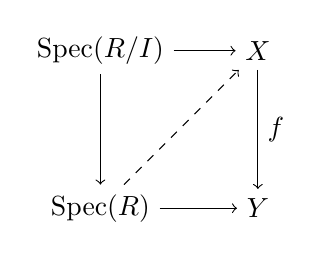
\begin{tikzpicture}
                \node (X) at (0, 1) {$X$};
                \node (Y) at (0, -1) {$Y$};
                \node (R) at (-2, -1) {$\mathrm{Spec}(R)$};
                \node (RI) at (-2, 1) {$\mathrm{Spec}(R/I)$};
                \draw[->] (X) -- node[right]{$f$} (Y);
                \draw[->] (RI) -- (X);
                \draw[->] (R) -- (Y);
                \draw[->] (RI) -- (R);
                \draw[->, dashed] (R) -- (X);
            \end{tikzpicture}
        \end{gather*}
        In other words, formally \'etale morphisms have the unique right lifting property with respect to infinitesimal thickenings. Analogously to the case of rings, the morphism $f$ is said to be \textbf{formally smooth} (resp.~\textbf{formally unramified}) if there is at least (resp.~at most) one lift.

        Since this definition does allow for some pathological examples, \'etale morphisms are those formally \'etale momorphisms that are locally of finite presentation.
    }

    \sremark{The term 'formally' should be interpreted in the sense of \textit{formal geometry} (see \cref{chapter:hdg}). There, infinitesimal neighbourhoods of points (see \ref{hdg:infinitesimal_thickening}), used for defining the local geometry, are induced by nilpotent ideals. This is further exemplified by \cref{alggeom:tangent_cone_etale}.}
    \begin{remark}
        As a side note, the general definition of \'etale morphism is related to \cref{alggeom:etale_morphism_variety}. The completion of the local ring $\mathcal{O}_x$ is defined by the inverse limit over the filtration $\mathcal{O}_x/\mathfrak{m}_x\leftarrow\mathcal{O}_x/\mathfrak{m}_x^2\leftarrow\mathcal{O}_x/\mathfrak{m}_x^3\leftarrow\cdots$. Hence, a morphism $\widehat{\mathcal{O}}_x\rightarrow\widehat{\mathcal{O}}_y$ between completions is characterized by consecutive lifting problems that are exactly the content of \cref{algebra:formally_etale}, since the ideals $\mathfrak{m}_x$ are clearly nilpotent in rings of the form $\mathcal{O}_x/\mathfrak{m}_x^k$ for any $k\in\mathbb{N}_0$.
    \end{remark}
    This is generalized to the schemes as follows.
    \begin{property}
        If $Y$ is locally Noetherian and $f:X\rightarrow Y$ is locally of finite presentation, \'etale morphisms can also be characterized in terms of completions. $f$ is \'etale if and only if the induced morphism on completions is formally \'etale in the adic topology.

        Moreover, if the induced morphisms of residue fields are isomorphisms, $f$ is \'etale if and only the induced morphisms of completions are isomorphisms (as in the case of affine varieties over algebraically closed fields).
    \end{property}

    \newdef{Finite \'etale morphism}{\index{etale!morphism}
        A morphism of schemes $f:X\rightarrow Y$ for which there exists a covering $\{U_i\}_{i\in I}$ of $Y$ by affine sets $U_i\equiv\mathrm{Spec}(A_i)$ such that $f^{-1}(U_i)\cong\mathrm{Spec}(B_i)$ is a free, separable $A_i$-algebra $B_i$ for all $i\in I$.
    }
    \begin{remark}[Finite \'etale covering]\index{etale!covering}
        When a finite \'etale morphism $f:X\rightarrow Y$ exists, $X$ is sometimes called a \textbf{finite \'etale cover(ing)} of $Y$. The full subcategory of the slice category $\mathbf{Sch}/_Y$ on finite \'etale coverings is often denoted by $\mathbf{FEt}_X$.
    \end{remark}

    \newdef{\'Etale fundamental group}{\index{fundamental group!etale}
        Consider a connected scheme $X$. The (\'etale) fundamental group $\pi_1(X)$ is the unique (up to isomorphism) profinite group \ref{topology:profinite_group} such that $\mathbf{FEt}_X$ is equivalent to the category $\mathbf{Fin}\,\pi_1(X)\mathbf{Set}$ of finite of $\pi_1(X)$-sets.
    }
    \begin{remark}
        Recall \cref{topology:equivalent_categories} for topological spaces. There, a stricter set of spaces was considered with the benefit that all $\pi_1(X)$-sets could be classified. By passing to profinite groups one can formulate a classification statement in the topological setting that is virtually identical to the above one.
    \end{remark}

\subsection{Tangent space}

    \newdef{Tangent cone}{\index{tangent!cone}\index{initial!part}
        Consider an affine variety $X=V(I)$. The tangent cone to $X$ at the origin is defined as the zero locus of the `initial ideal' of $I$:
        \begin{gather}
            C_0X := V\bigl(\{f^{\text{in}}\bigm\vert f\in I\}\bigr)\,,
        \end{gather}
        where $f^{\text{in}}$ denotes the \textbf{initial part} of $f$, i.e.~the sum of the smallest degree monomials in $f$.
    }

    \newdef{Tangent space}{\index{tangent!space}
        Consider an affine variety $X$ and choose a point $x\in X$. By working in a suitable affine chart, one can assume that $x=0$. This implies that any polynomial $f\in I(X)$ has a vanishing constant term. The tangent space at $x$ is defined as follows:
        \begin{gather}
            T_xX := V\bigl(\{f^{[1]}\bigm\vert f\in I(X)\}\bigr)\,,
        \end{gather}
        where $f^{[1]}$ denotes the linear part of the polynomial $f$.
    }
    \begin{property}
        For $x=0$ one obtains that $I(0)=(x_1,\ldots,x_n)/I(X)$. Moreover, there exists a natural isomorphism
        \begin{gather}
            I(0)/I(0)^2\cong\hom_K(T_0X,K)\,.
        \end{gather}
        The tangent space at $0$ can accordingly also be obtained as the dual of $I(0)/I(0)^2$.
    \end{property}

    It is not so hard to prove that this property can in fact easily be transported to arbitrary points $x\in X$ if one replaces the ideal $I(0)$ by the maximal ideal of the structure sheaf $\mathcal{O}_X$ at $x$. Therefore, one can give the following general definition.
    \newdef{Zariski tangent space}{\index{Zariski!tangent space}
        Consider a scheme $X$ with structure sheaf $\mathcal{O}_X$. At every point $x\in X$ the stalk $\mathcal{O}_x$ is a local ring and, hence, one obtain a maximal ideal $\mathfrak{m}_x$. The quotient $\mathfrak{m}_x/\mathfrak{m}_x^2$ is a vector space over the residue field $\mathcal{O}_x/\mathfrak{m}_x$. It is called the Zariski cotangent space at $x\in X$. Its algebraic dual is called the Zariski tangent space at $x\in X$.
    }
    \begin{property}[Inverse function theorem]\index{inverse function theorem}
        In the smooth setting (see \cref{chapter:manifolds} and onwards), the inverse function theorem states that a tuple of functions forms a local coordinate system at a point if their \textit{differentials} generate the \textit{cotangent space} at that point.

        Here, the ideal $\mathfrak{m}_x$ consists of the functions vanishing at $x\in X$ and the cotangent space is given by $\mathfrak{m}_x/\mathfrak{m}_x^2$. By Nakayama's lemma~\ref{algebra:nakayama}, a tuple of elements represent `coordinate functions', i.e.~generate $\mathfrak{m}_x$, if their `differential', i.e.~their residues in the Zariski cotangent space, generate the cotangent space.
    \end{property}

    \newdef{Regular scheme}{\index{regular!scheme}
        A (Noetherian) scheme is said to be regular or \textbf{nonsingular} if the local dimension at any point is equal to the dimension of the Zariski tangent space at that point. Equivalently, an affine variety is smooth if at every point the tangent space is isomorphic to the tangent cone.
    }

    \newadef{Tangent cone: Schemes}{\index{tangent!cone}
        Assume that $X$ is a Noetherian scheme. The tangent cone $C_xX$ is given by the spectrum of the graded ring $\mathrm{Gr}(\mathcal{O}_x)=\bigoplus_{k\in\mathbb{N}}\mathfrak{m}_x^k/\mathfrak{m}_x^{k+1}$. If $X$ is regular, the tangent cone coincides with the Zariski tangent space.
    }

    Recall \cref{alggeom:etale_morphism_variety} of \'etale morphisms of affine varieties (over algebraically closed fields). The following property relates these to the infinitesimal thickening point-of-view.
    \begin{property}\label{alggeom:tangent_cone_etale}
        A morphism $f:X\rightarrow Y$ of varieties induces an isomorphism on completions $\widehat{\mathcal{O}}_{f(x)}\rightarrow\widehat{\mathcal{O}}_x$ if and only if it induces an isomorphism on tangent cones.
    \end{property}

\section{\difficult{Sheaf theory}}

    This section also uses the content of \cref{chapter:topos}.

    \begin{property}[Coherent sheaves]
        A sheaf on a locally Noetherian scheme is coherent (\cref{sheaf:coherent}) if and only if it is quasicoherent and of finite type.
    \end{property}

    \newdef{Zariski topology}{\index{Zariski!topology}
        The Zariski topology on the category of schemes is generated by sets $\{f_i:U_i\rightarrow X\}_{i\in I}$ of open immersions such that $X=\bigcup_{i\in I}f_i(U_i)$ in the set-theoretic sense. This latter condition is often called \textbf{joint surjectivity}. This gives the \textbf{big Zariski site} on an a scheme $X$. The \textbf{small Zariski site} of a scheme $X$ is the subsite of $\mathbf{Sch}_{/X}$ on the open immersions.
    }
    \begin{remark}[Size issues]
        There are some size issues with the category of schemes, it being a big category. The result is that in general there exists no sheafification functor, i.e.~no general construction of the category of sheaves and, hence, this category can only be turned into a site, not a (Grothendieck) topos.\footnote{One can actually also work with large sites to obtain topoi as long as they contain a \textit{small topologically generating set} or, even more general, satisfy the \textit{WISC axiom}.} In the case of \textit{topological} or \textit{smooth manifolds}, this problem is often ignored since one has a (small) dense subsite and no issues arise. For schemes, however, the situation is different. For example, the fpqc topology (to be introduced below) does not admit a sheafification functor. Two solutions exists in such a context, either one works within a suitable universe or one only considers a single (pre)sheaf at a time.
    \end{remark}

    \begin{property}
        The Zariski site is subcanonical.
    \end{property}

    The following topology is finer than the Zariski topology.\footnote{There exists another topology in between the Zariski and \'etale topologies, the \textit{Nisnevich topology}, but this is of no interest here.}
    \newdef{\'Etale cover}{\index{cover!\'etale}\index{site!\'etale}
        An \'etale cover of a scheme $X$ is a jointly surjective family of \'etale morphisms that are locally of finite type\footnote{For $X$ locally Noetherian this additional condition is superfluous.}. The \textbf{big \'etale site} $\mathbf{Sch}_{/X,\text{\'et}}$ is the slice category of $X$ equipped with the coverage (see \cref{topos:coverage}) of \'etale covers. The \textbf{small \'etale site} is the subsite on \'etale morphisms.
    }

    \begin{property}
        A presheaf satisfies descent with respect to the \'etale topology if and only if it satisfies descent with respect to the following covers:
        \begin{itemize}
            \item Zariski covers, and
            \item (single) faithully flat morphisms of affine schemes.
        \end{itemize}
    \end{property}

    \newdef{Flat topologies}{\index{flat!topology}
        The finest topologies on the category of schemes (or slices thereof) are given by considering flat morphisms. The two most widely used flat topologies are the fppf and fpqc topologies. The \textbf{fppf topology} (for \textit{fid\`element plat de presentation finie}) is generated by jointly surjective families of flat morphisms that are locally of finite presentation. The \textbf{fpqc topology} (for \textit{fid\`element plat et quasi-compacte}) is generated by jointly surjective families of flat and quasicompact morphisms.
    }
    \begin{remark}
        With the definition as above the fpqc topology is technically not comparable to the Zariski topology since open immersions need not be quasicompact (unless one restricts to Noetherian schemes). A solution introduced by \textit{Vistoli} and \textit{Kleiman} is to replace quasicompactness by the following seemingly similar definition: There exists an open affine cover $\{U_i\}_{i\in I}$ of $X$ such that each $U_i$ is the image of a compact open subscheme. (If one drops the modifier `locally' in the definition of the fppf topology, a similar problem arises.)
    \end{remark}
    \begin{remark}[Standard covers]
        An equivalent approach to the definition of flat topologies is by first defining `standard' fppf or fpqc covers on affine schemes. These are similar to the flat covers defined above, but where the families are finite and the codomains affine. The covers of general schemes are then generated by base change.
    \end{remark}

    By interpreting objects in the big topos (over a scheme) as generalized spaces in the sense of \cref{chapter:hdg}, the following definition is obtained.
    \newdef{Algebraic space}{\index{algebraic!space}\index{atlas}\label{alggeom:algebraic_space}
        An object $X\in\mathbf{Sh}(\mathbf{Sch}_{\text{fppf}})$ satisfying
        \begin{enumerate}
            \item The diagonal morphism $X\rightarrow X\times X$ is representable (see \cref{topos:representable_diagonal}).
            \item There exists a scheme morphism $Y\rightarrow X$ that surjective and \'etale. This is sometimes called an \textbf{atlas}.
        \end{enumerate}
        Requiring representability of the diagonal can be argued as follows. The fibre product can be seen as a generalized notion of intersection, so representability means that the intersection of any two schemes is again a scheme. Moreover, representability of the diagonal also implies representability of the atlas morphism.
    }

    \newdef{Local property}{\index{local!property}\label{alggeom:local_property}
        Let $P$ be some property of scheme morphisms, e.g.~\'etale or smoothness. Relative to some topology on $\mathbf{Sch}$, the property $P$ is said to be \textbf{local on the source} if for every cover $\{X_i\rightarrow X\}_{i\in I}$ and every morphism $f:X\rightarrow Y$ the following holds:
        \begin{gather}
            f\text{ satisfies }P\iff\forall i\in I:X_i\rightarrow Y\text{ satisfies }P\,.
        \end{gather}
        Analogously, the property $P$ is said to be \textbf{local on the base} or \textbf{local on the target} if for every cover $\{Y_i\rightarrow Y\}_{i\in I}$ and every morphism $f:X\rightarrow Y$ the following holds:
        \begin{gather}
            f\text{ satisfies }P\iff\forall i\in I:Y_i\times_YX\rightarrow Y_i\text{ satisfies }P\,.
        \end{gather}
    }

    Inspired by locality one can generalize many properties of scheme morphisms to morphisms of algebraic spaces.
    \newdef{Property of algebraic spaces}{
        Consider a representable morphism of algebraic spaces $F:X\rightarrow Y$. If $P$ is a property of scheme morphisms satisfying:
        \begin{enumerate}
            \item it is preserved under base change, and
            \item it is fppf-local on the target,
        \end{enumerate}
        then $f$ is said to have the property $P$ if for all $T\in\ob{Sch}$ and all $G:h_T\rightarrow Y$ the morphism $S_G\rightarrow T$ has property $P$, where $S_G\in\ob{Sch}$ is a representing object of $G$, i.e.~$h_{S_G}\cong h_T\times_YF$.
    }
    \newdef{\'Etale morphism}{\index{etale!morphism}
        A morphism $F:X\rightarrow Y$ of algebraic spaces such that for every \'etale morphism $G:h_S\rightarrow X$ the composition $f\circ g$ is also \'etale.\footnote{In a similar vein, one can define smooth morphisms of algebraic spaces.}
    }

\section{Algebraic groups \& Galois theory}\index{Galois!theory}

    \newdef{Linear algebraic group}{
        A subgroup of $\GL(n,F)$ defined by a (finite) set of polynomials in the matrix coefficients.
    }
    \begin{property}
        From the definition, it is immediately clear that intersections of algebraic groups are again algebraic.
    \end{property}

    \newdef{Absolute Galois group}{
        The Galois group $\mathrm{Gal}(K_S/K)$ of the separable closure (\cref{algebra:separable_closure}) of $K$.
    }

    The following property relates Galois theory to algebraic geometry.
    \begin{property}[Grothendieck's Galois theory]\index{Grothendieck}
        Consider a field $K$ with separable closure $K_S$.
        \begin{gather}
            \mathrm{Gal}(K_S/K)\cong\pi_1\bigl(\mathrm{Spec}(K)\bigr)\,,
        \end{gather}
        where $\pi_1$ is the \'etale fundamental group (the fundamental group at the topological level would not carry a lot of information since $\mathrm{Spec}(K)$ is a one-point space).
    \end{property}

    \newdef{Abelian variety}{\index{variety!Abelian}
        A smooth, projective, algebraic group.
    }
    \begin{theorem}[Mordell--Weil]
        An Abelian variety $X$ over a number field $\mathfrak{K}$ (\cref{algebra:number_field}) such that its set of rational points $X(\mathfrak{K})$ (\cref{alggeom:rational_point_scheme}) is a finitely generated Abelian group.
    \end{theorem}

    \todo{COMPLETE}

\section{Tropical geometry}\index{tropical geometry}

    The following definition generalizes \cref{group:ring}.
    \newdef{Rig}{\index{rig}
        Let $R$ be a set equipped with two binary operations $+,\cdot$ (called\footnote{This might become confusing when looking at the examples below.} \textbf{addition} and \textbf{multiplication}). $(R,+,\cdot)$ is a rig if it satisfies the following axioms:
        \begin{enumerate}
            \item $(R,+)$ is a commutative monoid.
            \item $(R,\cdot)$ is a monoid.
            \item Multiplication is distributive with respect to addition.
        \end{enumerate}
    }
    \begin{remark}
        Whereas a ring is a group object in $\mathbf{CRing}$, a rig is a group object in $\mathbf{CMonoid}$. (The monoidal structures on these categories should not be taken to be the Cartesian ones for this result).
    \end{remark}

    \begin{example}[Tropical rig]
        Consider the set $T:=\mathbb{R}\cup\{+\infty\}$. This set becomes a rig when equipped with the following operations:
        \begin{enumerate}
            \item\textbf{Addition}: $x\oplus y=\min(x,y)$.
            \item\textbf{Multiplication}: $x\cdot y=x+y$.
        \end{enumerate}
    \end{example}

    \newdef{Tropicalization}{\index{tropicalization}\index{Puiseux series}
        In ordinary algebraic geometry, one considers polynomials over $\mathbb{R}$ as the basic building blocks. These also give rise to polynomials over $T$. To every polynomial
        \begin{gather}
            f = a+\sum_{i=1}^k\lambda_ix^{n_i}_i
        \end{gather}
        with $a\in\mathbb{Z}$, one assigns its tropicalization
        \begin{gather}
            \mathrm{trop}(f) := \min(0,n_1x_1,\ldots,n_kx_k)\,.
        \end{gather}
        Note that the tropicalization of any polynomial is a piecewise linear function.

        A more formal definition goes as follows. Let $K_P$ be the ring of \textbf{Puiseux series}, i.e.~of elements of the form
        \begin{gather}
            a = \sum_{i=k}^{+\infty}\lambda_ix^{i/n}
        \end{gather}
        for some $k,n\in\mathbb{N}$. These generalize Laurent series (\cref{complex:laurent_series}) to fractional exponents in that $K_P=\bigcup_{i\in\mathbb{N}_0}\mathbb{C}((x^{1/i}))$. Then, consider the valuation (\cref{algebra:valuation})
        \begin{gather}
            \mathrm{val}:K_P\rightarrow\mathbb{R}:a\mapsto\min\{i/k\mid\lambda_i\neq0\}\,.
        \end{gather}
        The tropicalization of
        \begin{gather}
            f = \sum_{u\in\mathbb{N}^n}\lambda_ux^u
        \end{gather}
        with $n\in\mathbb{N}$ is given by
        \begin{gather}
            \mathrm{trop}(f) := \min_{u\in\mathbb{N}^n,\lambda_u\neq 0}\bigl(\mathrm{val}(\lambda_u)+\sum_{i=1}^nu_ix_i\bigr)\,.
        \end{gather}
    }

    \todo{COMPLETE (link with mirror symmetry \citep{gross_tropical_2011})}
% \chapter{Number Theory}

    \minitoc

\section{Adic numbers}

    This section will make use of the content of \cref{section:stone_spaces}.

    \newdef{$p$-adic numbers}{\index{adic numbers}
        Consider a prime number $p\in\mathbb{N}$. For every $m,n\in\mathbb{N}$, one has that $\mathbb{Z}/p^n\mathbb{Z}\subseteq\mathbb{Z}/p^m\mathbb{Z}$ whenever $m\leq n$. The group $\mathbb{Z}_p$ of \textbf{$p$-adic integers} is given by the profinite group (\cref{topology:profinite_group}) obtained from this system of inclusions.

        Just like $\mathbb{Q}$ is the field of fractions (\cref{algebra:fraction_field}) of $\mathbb{Z}$ as in \cref{algebra:integers_rationals}, the $p$-adic numbers $\mathbb{Q}_p$ can be obtained as the field of fractions of $\mathbb{Z}_p$.
    }

    An alternative definition makes use of the notion of valuations (\cref{algebra:valuation}).
    \newadef{$p$-adic numbers}{\index{absolute value}
        Consider a prime number $p\in\mathbb{N}$. The $p$-adic valuation of an integer $z\in\mathbb{Z}$ is defined as follows:
        \begin{gather}
            \nu_p(z) :=
            \begin{cases}
                \max\{n\in\mathbb{N}:p^n\mid z\}&\cif z\neq0\,,\\
                +\infty&\cif z=0\,.
            \end{cases}
        \end{gather}
        This valuation extends to the rational numbers by taking
        \begin{gather}
            \nu_p\left(\frac{a}{b}\right) := \nu_p(a)-\nu_p(b)\,.
        \end{gather}
        In turn, the $p$-adic valuation also induces an \textit{absolute value} on $\mathbb{Z}$ (and on $\mathbb{Q}$) given by
        \begin{gather}
            |z|_p := p^{-\nu_p(z)}\,.
        \end{gather}
        The metric completions of $\mathbb{Z}$ and $\mathbb{Q}$ by these absolute values are the rings of $p$-adic integers and numbers, respectively.
    }
    \begin{remark}
        The $p$-adic valuation of a rational number $q\in\mathbb{Q}$ can also be defined as the (unique) integer $k\in\mathbb{Z}$ such that
        \begin{gather}
            q = p^k\frac{m}{n}
        \end{gather}
        for some integers $m,n\in\mathbb{Z}$ such that $p^k$, $m$ and $n$ are all coprime.
    \end{remark}

    \begin{theorem}[Ostrowski]\index{Ostrowski}
        The only nontrivial absolute values on $\mathbb{Q}$ are either the ordinary absolute value $|\cdot|$ or the $p$-adic absolute values $|\cdot|_p$.
    \end{theorem}

    \newdef{Profinite integers}{\index{integer!profinite}
        Similar to the construction of the $p$-adic integers, one can also construct the profinite completion (\cref{topology:profinite_completion}) of $\mathbb{Z}$. Instead of taking the inverse limit over the integers module a prime power, one simply takes the inverse limit over all finite cyclic groups:
        \begin{gather}
            \widehat{\mathbb{Z}} := \varprojlim_{n\in\mathbb{N}}\mathbb{Z}/n\mathbb{Z}\,.
        \end{gather}
        It can be shown that this is equivalent to taking the product of all $p$-adic integers:
        \begin{gather}
            \widehat{\mathbb{Z}}\cong\prod_{p\text{ is prime}}\mathbb{Z}_p\,.
        \end{gather}
    }

    \newdef{Adeles}{\index{adele}
        The ring of integral adeles is defined as the product
        \begin{gather}
            \mathbb{A}_{\mathbb{R}} := \mathbb{R}\times\widehat{\mathbb{Z}}\,.
        \end{gather}
        To obtain the proper ring of adeles, the above ring is rationalized:
        \begin{gather}
            \mathbb{A}_{\mathbb{Q}} := \mathbb{Q}\otimes_{\mathbb{Z}}\mathbb{A}_{\mathbb{R}}\,.
        \end{gather}
    }

\section{\difficult{Algebraic geometry}}

    This section gives a relation between number theory and (algebraic) geometry (\cref{chapter:alggeom}). The content of \namecrefs{chapter:complexcalculus}~\ref{chapter:algebra} and~\ref{chapter:complexcalculus} will also be used throughout this section.

\subsection{Modular forms}

    \newdef{Modular group}{\index{modular!group}\index{M\"obius transformation}\label{alggeom:modular_group}
        In the setting of number theory, the projective special linear group $\mathrm{PSL}(2,\mathbb{Z})$ is often called the modular group. The modular group acts on the complex plane by \textbf{M\"obius transformations}:
        \begin{gather}
            \begin{pmatrix}
                a&b\\
                c&d
            \end{pmatrix}
            z := \frac{az+b}{cz+d}\,.
        \end{gather}
        For this reason, $\mathrm{PSL}(2,\mathbb{C})$ is sometimes also called the \textbf{M\"obius group}.
    }

    \newdef{Modular form}{\index{modular!form}\index{cusp form}
        A modular form of weight $k\in\mathbb{R}$ is a holomorphic function on the upper-half plane $f:\mathcal{H}\rightarrow\mathbb{C}$ satisfying the following two conditions:
        \begin{enumerate}
            \item\textbf{Automorphicity}: For all $g\equiv\begin{pmatrix}a&b\\c&d\end{pmatrix}\in\mathrm{PSL}(2,\mathbb{Z})$, one has $f\bigl(g(z)\bigr)=(cz+d)^kf(z)$, and
            \item\textbf{Bounded growth}: $f(z)$ is bounded for $z\longrightarrow i\infty$.
        \end{enumerate}
        If the modular form satisfies the stronger condition $f(z)\longrightarrow0$ when $z\longrightarrow i\infty$, it is said to be \textbf{cuspidal} or it is simply called a \textbf{cusp form}.
    }
    \begin{remark}[Arithmetic group]\index{arithmetic group}
        Modular forms can also be defined for subgroups of $\mathrm{PSL}(2,\mathbb{Z})$ with finite index, the so-called \textbf{arithmetic groups}.
    \end{remark}

    \begin{property}
        The generators of the modular group are given by
        \begin{gather}
            z\mapsto-\frac{1}{z}\qquad\text{and}\qquad z\mapsto z+1\,.
        \end{gather}
        Invariance under the second generator shows that modular forms are, in particular, periodic and, hence, admit a Fourier expansion. Cusp forms are exactly those modular forms with vanishing constant Fourier coefficient.
    \end{property}

\subsection{Algebraic functions}

    \Cref{algebra:algebraic_element} can be generalized to the functional setting.
    \newdef{Algebraic function}{\index{algebraic!function}\index{transcendental!function}
        Let $R$ be a commutative ring. A function $f:R^n\rightarrow R$ is said to be algebraic if it is the solution of a polynomial equation with coefficients in $R[x_1,\ldots,x_n]$.\footnote{Often, the polynomial is required to be irreducible.} If $f$ is not algebraic, it is said to be \textbf{transcendental}.
    }

% \part{Higher Set Theory}
% \chapter{Topos theory}\label{chapter:topos}

    The main reference for this chapter is~\citet{johnstone_topos_2014,caramello_lectures_2019,caramello_topos-theoretic_2018,mac_lane_sheaves_1994}. For an introduction to stacks and descent theory, see~\citet{vistoli_notes_2004}.

    \minitoc

\section{Elementary topoi}

    \newdef{Subobject classifier}{\index{subobject!classifier}
        Consider a finitely complete category (in fact, the existence of a terminal object suffices). A subobject classifier is a mono\footnote{The symbol for this morphism will become clear in \cref{section:internal_logic}.} $\texttt{true}:1\hookrightarrow\Omega$ from the terminal object such that for every mono $\phi:x\hookrightarrow y$ there exists a unique morphism $\chi:y\rightarrow\Omega$ that fits in the following pullback square:
        \begin{figure}[ht!]
            \centering
            \begin{tikzpicture}
                \node (A) at (0, 0) {$x$};
                \node (B) at (0, -2) {$y$};
                \node (1) at (2, 0) {$1$};
                \node (O) at (2, -2) {$\Omega$};
                \node at (1, -1) {pb};
                \draw[->] (A) -- (1);
                \draw[right hook->] (A) -- node[left]{$\phi$} (B);
                \draw[right hook->] (1) -- node[right]{$\texttt{true}$} (O);
                \draw[->] (B) -- node[below]{$\exists!\chi$} (O);
            \end{tikzpicture}
            \caption{Subobject classifier.}
            \label{fig:subobject_classifier}
        \end{figure}
    }
    \begin{adefinition}
        Consider a well-powered category $\mathbf{C}$. The assignment of subobjects $\mathrm{Sub}(x)$ to an object $x\in\ob{C}$ defines functor $\mathrm{Sub}:\mathbf{C}^{op}\rightarrow\mathbf{Set}$. A subobject classifier $\Omega$ is a representation of this functor, i.e.~the following isomorphism is natural in $x$:
        \begin{gather}
            \mathrm{Sub}(x)\cong\mathbf{C}(x,\Omega)\,.
        \end{gather}
    \end{adefinition}

    \begin{example}[Indicator function]\index{indicator function}
        The category $\mathbf{Set}$ has the 2-element set $\{\texttt{true},\texttt{false}\}$ as subobject classifier. The morphism $\chi:S\rightarrow\Omega$ is the indicator function
        \begin{gather}
            \chi_S(x)=
            \begin{cases}
                \texttt{true}&\cif x\in S\,,\\
                \texttt{false}&\cif x\not\in S\,.
            \end{cases}
        \end{gather}
    \end{example}

    \newdef{Elementary topos}{\index{topos!elementary}
        An elementary topos is a finitely complete, Cartesian closed category (\cref{cat:closed}) admitting a subobject classifier. Equivalently, one can define an elementary topos as a finitely complete category that has all power objects exist.

        The power object $Px$ of $x\in\ob{\mathcal{E}}$ is related to the subobject classifier $\Omega$ by the following relation:
        \begin{gather}
            \label{topos:power_exponential}
            Px = \Omega^x\,.
        \end{gather}
    }
    \begin{remark}[Finite colimits]
        The original definition by \textit{Lawvere} also required the existence of finite colimits. However, it can be proven that finite cocompleteness follows from the other axioms.
    \end{remark}

    \begin{theorem}[Fundamental theorem of topos theory]\index{fundamental theorem!of topos theory}
        Let $\mathcal{E}$ be an elementary topos. The slice category $\mathcal{E}_{/x}$ is also a topos for every object $x\in\ob{\mathcal{E}}$. The subobject classifier is given by $\pi_2:\Omega\times x\rightarrow x$.
    \end{theorem}

    \begin{property}[Balanced]
        All monos in a topos are regular. Hence, every mono arises as an equalizer. Since, by \cref{cat:regular_iso}, every epic equalizer is necessarily an isomorphism, it follows that every topos is balanced (\cref{cat:balanced}).
    \end{property}

    \begin{property}[Epi/mono factorization]\index{image}
        Every morphism $f:x\rightarrow y$ in a topos factorizes uniquely as an epi followed by a mono:
        \begin{gather}
            x\overset{e}{\twoheadrightarrow}z\overset{m}{\hookrightarrow}y\,.
        \end{gather}
        The mono is called the \textbf{image} of $f$.
    \end{property}

\section{Morphisms}

    \newdef{Base change}{\index{base change}\label{topos:base_change}
        Consider a category $\mathbf{C}$ with pullbacks. For every morphism $f:x\rightarrow y$ one can define a functor $f^*:\mathbf{C}/y\rightarrow\mathbf{C}/x$. This functor acts by pullback along $f$.
    }
    \newdef{Dependent sum and product}{\index{dependent!sum/product}\label{topos:dependent_functors}
        Consider a base change functor $f^*$. The dependent sum and product functors are given by the right and left adjoints (if they exist):
        \begin{gather}
            \label{topos:dependent_adjoint_triple}
            \sum_f\dashv f^*\dashv \prod_f\,.
        \end{gather}
    }
    \begin{remark}
        The dependent sum can be shown to exist over any category. In fact, as a functor, it is simply given by postcomposition with $f$. However, the interpretation is much less trivial. Any morphism can be interpreted as a ``space'' with fibres the preimages. For example, in $\mathbf{Set}$, a morphism $g:Z\rightarrow X$ represents $Z$ as follows: \[Z\cong\bigsqcup_{x\in X}g^{-1}(x)\equiv\sum_{x:X}g^{-1}(x).\] The dependent sum generalizes this construction in a fibrewise manner, i.e.~the fibre over a point $y\in Y$ is given by
        \begin{gather}
            \sum_fg\,\Big|_y = \bigsqcup_{x\in f^{-1}(y)}g^{-1}(x)\,.
        \end{gather}
        Instead of combining all fibres into a single space, it combines those that lie in a single fibre of $f$.
    \end{remark}

    Although the dependent sum always exists, the dependent product requires more structure (see e.g.~\citet{huang_locally_2022}).
    \begin{property}[Locally Cartesian closed categories]
        In a locally Cartesian closed category (\cref{cat:closed}), all dependent products exist. In fact, the existence of the adjoint triple~\eqref{topos:dependent_adjoint_triple} is equivalent to $\mathbf{C}$ being locally Cartesian closed. For example, in $\mathbf{Set}$, the dependent product is given by
        \begin{gather}
            \label{topos:dependent_product_sets}
            \prod_fg\,\Big|_y=\prod_{x\in f^{-1}(y)}g^{-1}(x)\,.
        \end{gather}
        When $f$ is the terminal morphism, this represents the space of sections $X\rightarrow Z\equiv\sum_{x:X}g^{-1}(x)$ of $g$.

        More generally, the functor is obtained through the product-exponential adjunction in slice categories. The pullback is equal to a product in a slice category. Since $\mathbf{C}$ is locally Cartesian, one obtains for all $p:a\rightarrow y$ and $q:b\rightarrow y$:
        \begin{gather}
            \mathbf{C}_{/x}(p\times f,q)\cong\mathbf{C}_{/y}(p,q^f)
        \end{gather}
        for some morphism $q^f:b^f\rightarrow y$. Applying this exponential functor to the identity morphism $\mathbbm{1}_f$, gives a morphism $s:\mathbbm{1}_y\rightarrow f^f$ or $s:y\rightarrow x^f$ (this simply picks out the identity morphism in the exponential object internally). The dependent product is then defined as the pullback $\prod_fg:=s^*g^f$, where $g^f$ is interpreted as the morphism $(f\circ g)^f\rightarrow f^f$ in $\mathbf{C}_{/y}$.

        The idea behind this pullback construction is that in $\mathbf{Set}$, the pullback of $g^X:Z^X\rightarrow X^X$ along $s:\mathbbm{1}_X\rightarrow X^X$ is equal to the set
        \begin{gather}
            \{h\in Z^X\mid h\circ g=\mathbbm{1}_Z\}\,,
        \end{gather}
        i.e.~it consists of all sections of $g$. Hence, the pullback construction generalizes \cref{topos:dependent_product_sets}.
    \end{property}

    \newdef{Logical morphism}{\index{morphism!logical}
        A functor $f:\mathcal{E}\rightarrow\mathcal{F}$ between elementary topoi is said to be logical if it preserves finite limits, exponential objects and the subobject classifier.
    }
    \begin{property}
        If a logical morphism has a left adjoint if and only if it has a right adjoint.
    \end{property}

    \newdef{Geometric morphism}{\index{morphism!geometric}\index{direct!image}\index{inverse!image}
        A geometric morphism $f:\mathcal{E}\rightarrow\mathcal{F}$ of elementary topoi consists of an adjunction \[\mathcal{E}\adj{f^*}{f_*}\mathcal{F}\,,\] where the left adjoint is left exact. The right adjoint $f_*$ is called the \textbf{direct image} part of $f$ and the left adjoint $f^*$ is called the \textbf{inverse image} part. If $f^*$ itself has a left adjoint, then $f$ is said to be \textbf{essential}.
    }

    \newdef{Geometric surjection}{\index{surjective}
        A geometric morphism for which the inverse image part is faithful or, equivalently, reflects isomorphisms, is said to be \textbf{surjective} or is called a geometric surjection.
    }

    \newdef{Geometric embedding}{\index{embedding}\index{sub-!topos}\index{level}\label{topos:essential_subtopos}
        A geometric morphism for which the direct image part is fully faithful. If $\mathcal{E}\hookrightarrow\mathcal{F}$ is a geometric embedding, $\mathcal{E}$ is sometimes called a \textbf{subtopos} of $\mathcal{F}$. Moreover, if it is an essential geometric morphisms, the subtopos is itself said to be \textbf{essential}. Essential subtopoi $\mathcal{E}\hookrightarrow\mathcal{F}$ are also called \textbf{levels} of $\mathcal{F}$.
    }
    \begin{property}[Characterization of geometric embeddings]\label{topos:characterization_embedding}
        Let $f:\mathcal{E}\hookrightarrow\mathcal{F}$ be a geometric embedding and let $W\subset\mathrm{hom}(\mathcal{F})$ be the collection of morphisms that are mapped to isomorphisms under $f^*$. $\mathcal{E}$ is both equivalent to the full subcategory of $\mathcal{F}$ on $W$-local objects (\cref{cat:local_object}) and the \textit{localization} $\mathcal{F}[W^{-1}]$ at $W$ (see \cref{model:localization}).
    \end{property}

    \begin{property}[Base change]\index{base change}
        The base change functors on a topos are logical and admit a left adjoint, the postcomposition functor. This implies that these functors can be refined to essential geometric morphisms.
    \end{property}

    \begin{example}[Topological spaces]\label{topos:topological_spaces}
        Every continuous function $f:X\rightarrow Y$ induces a geometric morphism
        \begin{gather}
            \mathbf{Sh}(X)\adj{f^*}{f_*}\mathbf{Sh}(Y)\,,
        \end{gather}
        where the direct image functor $f_*$ is defined as
        \begin{gather}
            f_*F(U) := F(f^{-1}U)
        \end{gather}
        for any sheaf $F\in\mathbf{Sh}(X)$ and any open subset $U\in\mathbf{Open}(Y)$. The inverse image functor $f^*$ is defined using the equivalence between sheaves on topological spaces and \'etal\'e spaces. Consider a sheaf $E\in\mathbf{Sh}(Y)$ as an \'etal\'e space $\pi:E\rightarrow Y$. The inverse image of $E$ along a continuous function $f:X\rightarrow Y$ is the pullback of $\pi$ along $f$.
    \end{example}

    This example implies that the global elements $\ast\rightarrow X$ of a topological space induce geometric morphisms of the form $\mathbf{Sh}(\ast)\rightarrow\mathbf{Sh}(X)$. By noting that $\mathbf{Sh}(\ast)=\mathbf{Set}$, one obtains the following generalization.
    \newdef{Point}{\index{point}
        A point of a topos $\mathcal{E}$ is a geometric morphism $\mathbf{Set}\rightarrow\mathcal{E}$.
    }

    \newnot{Category of topoi}{
        The category of elementary topoi and geometric morphisms is a 2-category. It is denoted by $\mathbf{Topos}$.

        To obtain the structure of a 2-category, one needs to define an appropriate notion of 2-morphism. Because a geometric morphism consists of an adjunction, one can consider two distinct conventions. Either, one can choose the 2-morphisms in $\mathbf{Topos}$ to be the natural transformations $f^*\Rightarrow g^*$ (with associated transformations $g_*\Rightarrow f_*$) or, one can choose them to be the natural transformations $f_*\Rightarrow g_*$ (and associated transformations $g^*\Rightarrow f^*$). This chapter follows~\cite{johnstone_topos_2014} and the `inverse image convention' is used, i.e.~a 2-morphism $f\Rightarrow g$ consists of natural transformations $f^*\Rightarrow g^*$ and $g_*\Rightarrow f_*$.
    }

    \begin{property}[Balanced]
        The category $\mathbf{Topos}$ is balanced (\cref{cat:balanced}), i.e.~every geometric morphism that is both a geometric embedding and a geometric surjection is an equivalence. 
    \end{property}

    \begin{theorem}[Factorization]\index{factorization}
        Every geometric morphisms can be factorized as a geometric surjection followed by a geometric embedding.
    \end{theorem}

\section{Internal logic}\label{section:internal_logic}

    In this subsection, finitely complete categories that admit a subobject classifier are considered (they do not have to be elementary topoi).

    \newdef{Truth value}{\index{truth value}
        A global element of the subobject classifier, i.e.~a morphism $1\rightarrow\Omega$. The subobject classifier $\Omega$ is also sometimes called the \textbf{object of truth values}.
    }

    \begin{property}[Heyting algebra]\label{topos:heyting_algebra}
        For all objects $x$ in an elementary topos, the poset of subobjects $\mathrm{Sub}(x)$ has the structure of an internal meet-semilattice since forming pullbacks of monos gives a natural transformation
        \begin{gather}
            \cap_x:\hom(x,\Omega\times\Omega)\rightarrow\hom(x,\Omega)\,.
        \end{gather}
        By the Yoneda lemma, this induces an internal map
        \begin{gather}
            \land:\Omega\times\Omega\rightarrow\Omega\,.
        \end{gather}
        In fact, it can be shown that this gives the structure of an internal Heyting algebra (\cref{set:heyting}) and, in particular, that of an internal locale (\cref{topology:locale}). Hence, every topos canonically gives an external Heyting algebra, namely $\mathrm{Sub}(1)$. Furthermore, every power object is an internal Heyting algebra. This in particular includes the subobject classifier $\Omega=P1$.
    \end{property}

    \newdef{Mitchell--B\'enabou language}{\index{Mitchell--B\'enabou language}\index{proposition}\index{type}\index{variable}\index{term}
        Let $\mathcal{E}$ be an elementary topos with subobject classifier $\Omega$.
        \begin{enumerate}
            \item\textbf{Type}: An object $x\in\ob{\mathcal{E}}$.
            \item\textbf{Variable} (of type $x$): An identity morphism $\mathbbm{1}_x$.
            \item\textbf{Term} (of type $x$ in variables $\alpha_i$ of type $x_i$): a morphism $\prod_{i\in I}x_i\rightarrow x$.
            \item\textbf{Formula} or \textbf{proposition}: a term of type $\Omega$. Moreover, a formula is deemed true if it factors through $\mathtt{true}:1\rightarrow\Omega$.
        \end{enumerate}
        The logical connectives are induced by the internal Heyting structure on $\Omega$. Quantifiers are induced by the (internal) completeness of $\Omega$.

        Every type also comes equipped with two binary relations:
        \begin{enumerate}
            \item $=_x$ is obtained from the characteristic morphism of the diagonal inclusion.
            \item $\in_x$ is obtained by using the evalution map of the exponential object together with \cref{topos:power_exponential}.
        \end{enumerate}
        Since the slices of an elementary topos are themselves elementary topoi, one can also define dependent types. An \textbf{indexed type} is an object of a slice category. \textbf{(Dependent) sums} and \textbf{products} of type families are goven by the left and right adjoints to the base change functor.
    }

    An interpretation of the Mitchell--B\'enabou language in an elementary topos $\mathcal{E}$ goes as follows.
    \newdef{Kripke--Joyal semantics}{\index{Kripke--Joyal semantics}\index{entailment}
        The \textbf{entailment} $U\vdash\phi(\alpha)$ for a term $\alpha:U\rightarrow X$ and a proposition $\phi(x):X\rightarrow\Omega$ is said to hold if $\alpha$ factors through the pullback $\{x\in X\mid\phi(x)\}$.
    }

    \begin{property}[Monotonicity]
        If $V\vdash\phi(\alpha)$ and $f:U\rightarrow V$, then $U\vdash\phi(\alpha\circ f)$.
    \end{property}
    \begin{property}[Locality]
        If $f:U\rightarrow V$ is epic and $V\vdash\phi(\alpha\circ f)$, then $U\vdash\phi(\alpha)$.
    \end{property}

    \todo{COMPLETE}

\section{Grothendieck topoi}\label{section:grothendieck_topos}
\subsection{Grothendieck topologies}

    \newdef{Sieve}{\index{sieve}
        Let $\mathbf{C}$ be a small category. A sieve $S$ on $\mathbf{C}$ is a fully faithfull discrete fibration $S\hookrightarrow\mathbf{C}$.

        A sieve $S$ on an object $x\in\mathbf{C}$ is a sieve in the slice category $\mathbf{C}_{/x}$. This means that $S$ is a subset of $\mathrm{ob}(\mathbf{C}_{/x})$ that is closed under precomposition, i.e.~if $y\rightarrow x\in S$ and $z\rightarrow y\in\mathrm{hom}(\mathbf{C})$, then $z\rightarrow y\rightarrow x\in S$.

        All of this can be summarized by saying that a sieve on an object $x\in\ob{C}$ is a subfunctor of the hom-functor $\mathbf{C}(-,x)$.
    }

    \begin{example}[Maximal sieve]
        Let $\mathbf{C}$ be a category. The maximal sieve on $x\in\ob{C}$ is the collection of all morphisms $\{f\in\mathrm{hom}(\mathbf{C})\mid\cod(f)=x\}$ or, equivalently, all of $\mathrm{ob}(\mathbf{C}_{/x})$.
    \end{example}
    \begin{example}[Pullback sieve]
        Consider a morphism $f:x\rightarrow y$. Given a sieve $S$ on $y$, one can construct the pullback sieve $f^*S$ on $x$ as the sieve of morphisms in $S$ that factor through $f$:
        \begin{gather}
            f^*S(x) = \bigl\{g\bigm\vert f\circ g\in S(y)\bigr\}\,.
        \end{gather}
    \end{example}

    \newprop{Presheaf topos}{\index{presheaf!topos}\label{topos:presheaf_topos}
        Consider the presheaf category $\mathbf{Psh}(\mathbf{C})$ on an arbitrary (small) category $\mathbf{C}$. This category is an elementary topos, where the subobject classifier assigns sieves:
        \begin{gather}
            \underline{\Omega}(x) := \{S\mid S\text{ is a sieve on }x\}\,.
        \end{gather}
        The action on a morphism $f:x\rightarrow y$ gives the morphism $\underline{\Omega}(f)$ that sends a sieve $S$ to its pullback sieve $f^*S$.

        The morphism $\texttt{true}:\underline{1}\hookrightarrow\underline{\Omega}$ is defined as the natural transformation assigning to every object its maximal sieve. For every subobject $\underline{Y}\hookrightarrow\underline{X}$ the characteristic morphism $\chi_{_{\underline{Y}}}$ is defined as follows. Consider an object $c\in\ob{C}$. The component $\chi_{_{\underline{Y}}}|_c$ is then given by
        \begin{gather}
            \chi_{_{\underline{Y}}}|_c(x) := \bigl\{f\in\mathbf{C}(d,c)\mid\underline{X}(f)(x)\in\underline{Y}(d)\bigr\}\,,
        \end{gather}
        for all $x\in\underline{X}(c)$.
    }

    The following definition is due to \textit{Giraud} (for the original definition using the notion of a \textit{cover}, see the end of this section).
    \newdef{Grothendieck topology}{\index{Grothendieck!topology}\index{covering!sieve}\label{topos:grothendieck_topology}
        A Grothendieck topology on a category $\mathbf{C}$ is a map $J$ assigning to every object a collection of sieves satisfying the following conditions:
        \begin{enumerate}
            \item\textbf{Identity}\footnote{The name itself stems from the fact that the maximal sieve is generated from the identity morphism.}: For every object $x\in\ob{C}$, the maximal sieve $M_x$ is an element of $J(x)$ or, equivalently, all sieves generated by isomorphisms are in $J(x)$.
            \item\textbf{Base change}: If $S\in J(x)$, then $f^*S\in J(y)$ for every morphism $f:y\rightarrow x$.
            \item\textbf{Locality}: Consider a sieve $S$ on $x\in\ob{C}$. If there exists a sieve $R\in J(x)$, such that for every morphism $(f:y\rightarrow x)\in R$ the pullback sieve $f^*S\in J(y)$, then $S\in J(x)$.
        \end{enumerate}
        The sieves in $J$ are called ($J$-)\textbf{covering sieves}. A collection of morphisms with codomain $x\in\ob{C}$ is called a \textbf{cover}\footnote{Sometimes this term is also used to denote any collection of morphism with common codomain $x$, i.e.~without reference to a covering sieve.} of $x$ if the sieve generated by these morphisms is a covering sieve on $x$.
    }

    \begin{example}[Topological spaces]
        These conditions have the following interpretation in the case of topological spaces:
        \begin{itemize}
            \item The collection of all open subsets covers a space $U$.
            \item If $\{U_i\}_{i\in I}$ covers $U$, then $\{U_i\cap V\}_{i\in I}$ covers $U\cap V$.
            \item If $\{U_i\}_{i\in I}$ covers $U$ and, if for every $i\in I$ the collection $\{U_{ij}\}_{j\in J_i}$ covers $U_i$, then $\{U_{ij}\}_{i\in I,j\in J_i}$ covers $U$.
        \end{itemize}
        The canonical Grothendieck topology on $\mathbf{Open}(X)$ is given by the sieves $S=\{U_i\hookrightarrow U\}_{i\in I}$, where $\bigcup_{i\in I}U_i=U$. This topology is denoted by $J_{\mathbf{Open}(X)}$.
    \end{example}

    \newdef{Site}{\index{site}
        A (small) category equipped with a Grothendieck topology $J$.
    }

    A slightly weaker notion than that of a (Grothendieck) topology is the following.
    \newdef{Coverage}{\index{coverage}\index{cover}\label{topos:coverage}
        Let $\mathbf{C}$ be a category. A coverage on $\mathbf{C}$ is a map that assigns to every object $x\in\ob{C}$ a collection of families $\{f:y\rightarrow x\}\subset\mathrm{hom}(\mathbf{C})$, the \textbf{covering families} or \textbf{covers}, satisfying the following condition. If $\{f:y\rightarrow x\}$ is a covering family on $x$, then for every morphism $g:x'\rightarrow x$ there exists a covering family $\{f':y'\rightarrow x'\}$ on $x'$ such that every composite $g\circ f'$ factors through some $f$.
    }

    \newdef{Matching family}{\index{matching!family}\label{topos:matching_family}
        Consider a presheaf $F\in\mathbf{Psh(C)}$ together with a sieve $S$ on $x\in\ob{C}$. A matching family for $S$ with respect to $F$ is a natural transformation $\alpha:S\Rightarrow F$ between $S$, regarded as a subfunctor of $\mathbf{C}(-,x)$, and $F$.

        More explicitly, it is an assignment of an element $x_f\in Fy$ to every morphism $(f:y\rightarrow x)\in S$ such that
        \begin{gather}
            F(g)(x_f) = x_{f\circ g}
        \end{gather}
        for all morphisms $g:z\rightarrow y$. Equivalently, a matching family for $S$ with respect to $F$ is a set of elements $\{x_f\}_{f\in S}$ such that for all covering morphisms $f:y\rightarrow x,g:z\rightarrow x\in S$ and all morphisms $f':c\rightarrow y, g':c\rightarrow z$ such that $f\circ f'=g\circ g'$ the following equations holds:
        \begin{gather}
            \label{topos:matching_family_condition}
            F(f')(x_f)=F(g')(x_g)\,.
        \end{gather}
        Given such a matching family, one calls an element $a\in Fx$ an \textbf{amalgamation} if it satisfies
        \begin{gather}
            F(f)(a)=x_f
        \end{gather}
        for all morphisms $f\in S(y)$.
        
        The existence of such an element can also be stated in terms of natural transformations. Consider the obvious inclusion $\iota_S$ of $S$ into the the hom-functor $\mathbf{C}(-,x)$. Every morphism with codomain $x$ can be obtained from the identity morphism by precomposition and, hence, a natural transformation $\mathbf{C}(-,x)\Rightarrow F$ is determined by its action on the identity morphisms $\mathbbm{1}_x$. The existence of an amalgamation is thus equivalent to the existence of an extension of $S$ along $\iota_S$.
    }
    \remark{If the base category has all pullbacks, for example if it is a topos on its own, one can restrict the above commuting diagrams to the pullback diagrams of morphisms in the sieve $S$.}

    \newdef{Sheaf}{\index{sheaf}\index{presheaf!separated}\label{topos:sheaf}
        Consider a site $(\mathbf{C},J)$. A presheaf $F$ on $\mathbf{C}$ is called a $J$-sheaf if every matching family, for every covering sieve in $J$, admits a unique amalgamation\footnote{If there exists at most one amalgamation, the presheaf is said to be \textbf{separated}.} or, equivalently, if all sieves admit a unique extension to representable presheaves.

        The category $\mathbf{Sh}(\mathbf{C},J)$ of $J$-sheaves on the site $(\mathbf{C},J)$ is the full subcategory of $\mathbf{Psh(C)}$ on the presheaves that satisfy the above condition.
    }
    This definition can also be restated in terms of local objects (\cref{cat:local_object}).
    \newadef{Sheaf}{\index{descent}\label{topos:local_object_sheaf}
        By definition every covering sieve admits a morphism into the Yoneda embedding: $\eta:S\hookrightarrow\mathcal{Y}x$. If the collection of all these morphisms is denoted by $\mathcal{S}$, a presheaf is a sheaf if and only if it is $\mathcal{S}$-local, i.e.~if the following morphism is an isomorphism for all $\eta\in\mathcal{S}$:
        \begin{gather}
            Fx\cong\mathbf{Psh}(\mathcal{Y}x,F)\xrightarrow{\mathbf{Psh}(\eta, F)}\mathbf{Psh}(S,F)\,.
        \end{gather}
        This is also called the \textbf{descent condition} for sheaves. In this context the collection of matching families $\mathrm{Match}(S,F):=\mathbf{Psh}(S,F)$ for a sieve $S$ with respect to a presheaf $F$ is often called the \textbf{descent object} of $S$ with respect to $F$.
    }

    \begin{example}[Topological spaces]\index{topos!spatial}
        The usual category of sheaves $\mathbf{Sh}(X)$ on a topological space $X$ is obtained as the category of sheaves on the site $(\mathbf{Open}(X),J_{\mathbf{Open}(X)})$. A Grothendieck topos of this form is also called a \textbf{spatial topos}. Since the morphisms in the covering sieves are exactly the inclusion maps $U_i\hookrightarrow U$, the pullback of two such morphisms is given by the intersection $U_i\cap U_j$. Hence, the condition for a matching family, as formulated in \cref{topos:matching_family} above, gives the second part of \cref{sheaf:def}. The uniqueness of an amalgamation is equivalent to the first part of that definition.

        For topological spaces, sheaves are easily represented visually. A matching family assigns to every set $U_i$ of an open cover $\mathcal{U}\equiv\{U_i\}_{i\in I}$ of $U$ an element $x_i\in FU_i$, such that the restrictions coincide on double overlaps, as in step $(1)$ in the figure below.
        \begin{gather*}
            \begin{tikzpicture}[baseline=-1mm]
                \node (title) at (0, 2) {Cover};
                \node (Uij) at (0, 1) {$U_i\cap U_j$};
                \node (Ui) at (-1, 0) {$U_i$};
                \node (Uj) at (1, 0) {$U_j$};
                \node (U) at (0, -1) {$U$};
                \draw[left hook->] (Uij) -- (Ui);
                \draw[right hook->] (Uij) -- (Uj);
                \draw[right hook->] (Ui) -- (U);
                \draw[left hook->] (Uj) -- (U);
            \end{tikzpicture}
            \xrightarrow{\ (1)\ }
            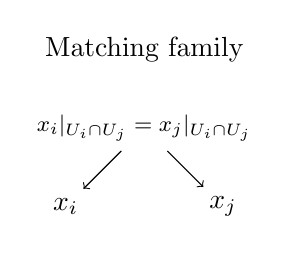
\begin{tikzpicture}[baseline=-1mm]
                \node (title) at (0, 2) {Matching family};
                \node (Uij) at (0, 1) {\footnotesize$x_i|_{U_i\cap U_j} = x_j|_{U_i\cap U_j}$};
                \node (Ui) at (-1, 0) {$x_i$};
                \node (Uj) at (1, 0) {$x_j$};
                \draw[->] (Uij) -- (Ui);
                \draw[->] (Uij) -- (Uj);
            \end{tikzpicture}
            \xrightarrow{\ (2)\ }
            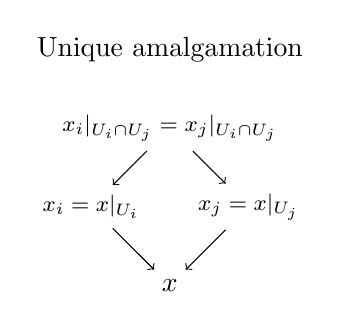
\begin{tikzpicture}[baseline=-1mm]
                \node (title) at (0, 2) {Unique amalgamation};
                \node (Uij) at (0, 1) {\footnotesize$x_i|_{U_i\cap U_j} = x_j|_{U_i\cap U_j}$};
                \node (Ui) at (-1, 0) {\footnotesize$x_i=x|_{U_i}$};
                \node (Uj) at (1, 0) {\footnotesize$x_j=x|_{U_j}$};
                \node (U) at (0, -1) {$x$};
                \draw[->] (Uij) -- (Ui);
                \draw[->] (Uij) -- (Uj);
                \draw[->] (Ui) -- (U);
                \draw[->] (Uj) -- (U);
            \end{tikzpicture}
        \end{gather*}
        The descent condition then states that for every such matching family, there exists a unique element $x$ on $U$, such that the elements of the matching family are restrictions of $x$ as in step $(2)$ of the figure above.

        The classical example would be the assignment of the set of continuous functions to open subsets of a topological space. When two functions, defined on two open sets, coincide on the intersection, there exists a unique continuous function defined on the union, such that it restricts to the given functions.
    \end{example}

    Above, in \cref{topos:coverage}, the notion of a coverage was introduced. It should be clear that every coverage generates a sieve. Furthermore, although coverages are weaker and easier to handle, they are in fact equivalent for the purpose of sheaf theory.
    \begin{property}
        Consider a covering family $C$ and let $S_C$ be the sieve it generates. A presheaf is a sheaf for $C$ if and only if it is a sheaf for $S_C$.
    \end{property}

    \begin{example}[Canonical topology]\index{topology!canonical}
        The canonical topology on a category is the finest Grothendieck topology for which all representable presheaves are sheaves. A \textbf{subcanonical topology} is then defined as a subtopology of the canonical one, i.e.~any Grothendieck topology for which all representable presheaves are sheaves.
    \end{example}
    \begin{example}[Minimal and maximal topologies]
        The minimal Grothendieck topology on a category is the one for which only the maximal sieves are covering sieves. In this topology all presheaves are sheaves. The maximal Grothendieck topology is the one for which all sieves are covering sieves. In this topology only the terminal element of the associated presheaf category is a sheaf.
    \end{example}

    \newdef{Grothendieck topos}{\index{Grothendieck|seealso{topos}}\index{topos!Grothendieck}
        A category equivalent to the category of sheaves on a (small) site. This site is often called the \textbf{site of definition} for the given topos.
    }
    \begin{property}
        Every Grothendieck topos is an elementary topos.
    \end{property}

    \begin{property}
        For every Grothendieck topos, there exists a (standard) site of definition for which the Grothendieck topology is (sub)canonical.
    \end{property}
    \begin{property}
        Let $\mathcal{E}$ be a Grothendieck topos. The canonical topology $J_{\text{can}}$ on $\mathcal{E}$ is the topology for which the covering sieves are jointly epimorphic families. Moreover,
        \begin{gather}
            \mathcal{E}\cong\mathbf{Sh}(\mathcal{E},J_{\text{can}})\,.
        \end{gather}
    \end{property}

    \begin{construct}[Sheafification]\index{sheafification}
        Given a presheaf $\mathcal{F}$, one can construct a sheaf $\overline{\mathcal{F}}$ along the same lines of \cref{sheaf:colimit_construction}.
    \end{construct}

    \newdef{Global sections functor}{\index{global!sections}\label{topos:global_sections}
        Every Grothendieck topos $\mathcal{E}$ admits a geometric morphism to $\mathbf{Set}$, where the right adjoint assigns to an object $x$ its set of global elements:
        \begin{gather}
            \Gamma:\mathcal{E}\rightarrow\mathbf{Set}:x\mapsto\mathcal{E}(1,x)\,.
        \end{gather}
        When $\mathcal{E}$ is the sheaf topos over a topological space, this is exactly the global sections functor (\cref{sheaf:global_sections_functor}). The left adjoint assigns to every set $S$ the copower $S\cdot1\equiv\bigsqcup_{s\in S}1$. When $\mathcal{E}$ is a sheaf topos, this adjoint is exactly the constant sheaf functor. It is sometimes denoted by $\mathrm{LConst}$ (cf.~\cref{sheaf:constant_sheaf}).
    }

    A different approach for defining sheaf topoi is through an embedding of sheaves into presheaves.
    \newdef{Local isomorphism}{\index{local!isomorphism}
        A system of local isomorphisms in $\mathbf{Psh(C)}$ is a class of morphisms in $\mathbf{Psh(C)}$ forming a \textit{system of weak equivalences} (see \cref{model:weak_equivalence}) closed under pullbacks along morphisms out of representable presheaves.
    }
    \begin{property}[Local isomorphisms and Grothendieck topologies]
        A system of local isos induces a \textit{system of local epis} in the following way. $f:X\rightarrow Y$ is a local epi if $\im(f)\rightarrow Y$ is a local iso. A Grothendieck topology is defined by declaring a presheaf $F\in\mathbf{Psh(C)}$ to be a covering sieve at $X\in\ob{C}$ if $F\hookrightarrow\mathcal{Y}X$ is a local epi.
    \end{property}

    \newadef{Sheaf topos}{\index{topos!sheaf}\label{topos:topos_geometric_embedding}
        A category $\mathbf{Sh(C)}$ equipped with a geometric embedding into $\mathbf{Psh(C)}$.
        \begin{mdframed}[roundcorner=10pt, linecolor=blue, linewidth=1pt]
            \begin{proof}[Proof of equivalence]
            By \cref{topos:characterization_embedding}, such a category is equivalent to the full subcategory on $S$-local presheaves for some system of local isomorphisms $S$ and, therefore, also to a sheaf topos in the sense of Grothendieck by the property above.
            \end{proof}
        \end{mdframed}
    }

    \begin{remark}[Descent condition]
        This is essentially a restatement of the descent condition (cf.~\ref{topos:local_object_sheaf}). Covering sieves, regarded as subfunctors, are in particular local isomorphisms. Stability of sieves under pullback, together with the co-Yoneda lemma~\ref{cat:ninja_yoneda}, which says that every presheaf is a colimit of representables, generates the full collection of local isomorphisms.
    \end{remark}

    The characterization of geometric embeddings and, hence, of Grothendieck topoi in terms of \textit{localizations} (\cref{topos:characterization_embedding}) is equivalent to a definition in terms of reflections (this is due to \textit{Street}).
    \begin{result}
        There exists a bijection between the Grothendieck topologies on a small category $\mathbf{C}$ and the equivalence classes of left exact reflective subcategories of $\mathbf{Psh(C)}$.
    \end{result}

    \newdef{Representable morphism}{\index{representable}
        A natural transformation of presheaves $F\rightarrow G$ is said to be representable if, for every representable presheaf $h_X$ and every morphism $h_X\rightarrow G$, the pullback $h_X\times_GF$ is representable.
    }

    \begin{property}[Diagonals]\label{topos:representable_diagonal}
        The diagonal morphism $\Delta_F:F\rightarrow F\times F$, for $F$ a presheaf on a category with pullbacks, is representable if and only if any of the following two equivalent properties holds:
        \begin{enumerate}
            \item For every two representable presheaves $h_X,h_Y$ and natural transformations $h_X\rightarrow F,h_Y\rightarrow F$, the pullback $h_X\times_Fh_Y$ is representable.
            \item Every natural transformation $h_X\rightarrow F$ from a representable presheaf is representable.
        \end{enumerate}
    \end{property}

\subsection{Topological sheaves}

    See \cref{chapter:sheaf} for the application of sheaves to topology.

    \begin{property}[Presheaf topos]\label{topos:sheaf_topos}
        Consider the presheaf category
        \begin{gather}
            \mathbf{Psh}(X):=\mathbf{Psh\bigl(Open}(X)\bigr)
        \end{gather}
        over a topological space $(X,\tau)$. Unpacking \cref{topos:presheaf_topos} shows that this category is an elementary topos where the subobject classifier is given by
        \begin{gather}
            \Omega(U) = \{V\in\tau\mid V\subseteq U\}\,.
        \end{gather}
    \end{property}

    \begin{construct}[Sheaves and \'etale bundles]\index{bundle}\label{topos:etale_adjunction}
        Let $X$ be a topological space. The functor
        \begin{gather}
            I:\mathbf{Open}(X)\rightarrow\mathbf{Top}_{/X}:U\mapsto(U\hookrightarrow X)
        \end{gather}
        induces the following adjunction:
        \begin{gather}
            \mathbf{Top}_{/X}\adj{E}{\Gamma}\mathbf{Psh}(X)\,.
        \end{gather}
        The slice category on the left-hand side is the category of (topological) \textit{bundles} (see \cref{chapter:bundles}) over $X$. Both directions of the adjunction have a clear interpretation. The right adjoint assigns to every bundle its sheaf of local sections and the left adjoint assigns to every presheaf its bundle of germs.

        By restricting to the subcategories on which this adjunction becomes an adjoint equivalence, one obtains the \textbf{\'etale space} and \textbf{sheaf categories} respectively:
        \begin{gather}
            \mathbf{Et}(X)\cong\mathbf{Sh}(X)\,.
        \end{gather}
        The category on the right-hand side is the category of sheaves on a topological space $X$. The category on the left is the full subcategory on local homeomorphisms, i.e.~the \'etale spaces (\cref{topology:etale_space}).
    \end{construct}

    \begin{property}[Associated sheaf]
        The inclusion functor $\mathbf{Sh}(X)\hookrightarrow\mathbf{Psh}(X)$ admits a left adjoint, the \textbf{sheafification functor}, that assigns to every presheaf its associated sheaf. This functor is given by the composition $\Gamma\circ E$, which is simply \cref{sheaf:etale_construction}.

        The fact that the counit of the adjunction (\cref{topos:etale_adjunction}) restricts to an isomorphism on the full subcategory $\mathbf{Sh}(X)$ is equivalent to the fact that the sheafification of a sheaf $\Gamma$ is again $\Gamma$.
    \end{property}

    \newdef{Petit and gros topoi\footnotemark}{\index{topos!petit \& gros}\index{topos!spatial}
        \footnotetext{For those that do not master French, `\textit{petit}' and `\textit{gros}' mean small and big, respectively.}
        Consider a topological space $X$ together with its category of opens $\mathbf{Open}(X)$. The petit topos over $X$ is defined as the sheaf topos $\mathbf{Sh}(X)\equiv\mathbf{Sh}\bigl(\mathbf{Open}(X)\bigr)$. It represents $X$ as a `generalized space'. (By \cref{topos:etale_adjunction}, the objects in a petit topos are the \'etale spaces over the given base space.) Topoi equivalent to such petit topoi are sometimes said to be \textbf{spatial}. However, one can also build a topos whose objects are themselves generalized spaces. To this end, choose a site $S$ of `probes' and call the sheaf topos $\mathbf{Sh}(S)$ a gros topos. (See \cref{section:smooth_spaces} for more information.)
    }

    \begin{property}[Localic reflection]\index{localic!reflection}
        Mapping a topological space to its sheaf of continuous sections defines a functor $\func{\mathbf{Sh}}{Top}{Topos}$ by \cref{topos:topological_spaces}. When restricted to the full subcategory of sober spaces (\cref{topology:sober_space}), this functor becomes fully faithful. Generalizing to locales even gives a reflective inclusion (\cref{cat:reflective_inclusion}).

        This property states that no information is lost when regarding (sober) topological spaces as sheaf topoi. This also explains the name `petit topos'.
    \end{property}

    \newdef{Localic topos}{\index{localic!topos}
        Multiple equivalent definitions exist:
        \begin{enumerate}
            \item A topos equivalent to a sheaf topos over a locale (\cref{topology:locale}) equipped with the topology of jointly surjective morphisms.
            \item A topos generated under colimits of subobjects of the terminal object $1$.
            \item A topos $\mathcal{E}$ for which the global sections functor $\Gamma:\mathcal{E}\rightarrow\mathbf{Set}$ is localic, i.e.~every object in $\mathcal{E}$ is a subquotient of an object in the inverse image $\Gamma^*$
        \end{enumerate}
        Given a geometric morphism to some base topos $\mathcal{S}$, one can define $\mathcal{S}$-localic topoi by generalizing the third point.
    }
    The following property shows that the locale in the first definition has a specific meaning.
    \begin{property}
        By \cref{topos:heyting_algebra}, for every topos the poset $\mathrm{Sub}(1)$ is a locale. Every localic topos $\mathcal{E}$ satisfies $\mathcal{E}\cong\mathrm{Sh}\bigl(\mathrm{Sub}(1)\bigr)$, where $\mathrm{Sub}(1)$ is equipped with the topology of jointly surjective morphisms.
    \end{property}

    The equivalence between localic topoi and locales carries over to the notion of $\mathcal{S}$-localic topoi.
    \begin{property}
        The (2-)category of localic topoi over a base topos $\mathcal{S}$ is equivalent to the (2-)category $\mathbf{Loc}(\mathcal{S})$ of locales internal to $\mathcal{S}$.
    \end{property}
    \begin{property}\label{topos:slice_locale}
        Given a locale $X$, the category $\mathbf{Loc}\bigl(\mathbf{Sh}(X)\bigr)$ is equivalent to the slice category $\mathbf{Loc}_{/X}$.
    \end{property}

\subsection{Lawvere--Tierney topology}

    This section gives an alternative approach to the construction of sheaf topoi, which is more closely linked to the logical aspect of topos theory.

    \newdef{Lawvere--Tierney topology}{\index{Lawvere--Tierney}
        As noted in \cref{section:internal_logic} on the internal logic of elementary topoi, the subobject classifier $\Omega$ has the structure of an internal Heyting algebra and, in particular, that of a (bounded) meet-semilattice. This internal poset, viewed as an internal category, admits the construction of a closure operator $j:\Omega\rightarrow\Omega$ (\cref{cat:closure_operator}) satisfying the following condition:
        \begin{gather}
            j\circ\land = \land\circ(j\times j)\,.
        \end{gather}
        This condition states (in a nontrivial way) that $j$ is (internally) order-preserving. More concisely, a Lawvere--Tierney topology is internally a left exact modality on $\Omega$.
    }
    \begin{remark}
        The condition satisfied by the unit morphism in the definition of a closure operator can also be reformulated in this context as follows:
        \begin{gather}
            j\circ\texttt{true} = \texttt{true}\,.
        \end{gather}
    \end{remark}

    \begin{example}[Double negation topology]\index{topology!double negation}\label{topos:double_negation}
        As mentioned above, the subobject classifier in an elementary topos has the structure of an internal Heyting algebra and, hence, admits a negation morphism $\lnot:\Omega\rightarrow\Omega$. It can be shown that double negation $\lnot\lnot:\Omega\rightarrow\Omega$ gives a Lawvere--Tierney topology.
    \end{example}
    \begin{property}\index{Booleanization}\index{Boolean!subtopos}\index{dense!subtopos}
        The Booleanization $\mathcal{E}_{\lnot\lnot}\hookrightarrow\mathcal{E}$ of an elementary subtopos is the smallest dense subtopos of $\mathcal{E}$ and the largest Boolean subtopos of $\mathcal{E}$, i.e.~it is the unique subtopos such that:
        \begin{enumerate}
            \item\textbf{Dense}: $\mathcal{E}_{\lnot\lnot}$ contains the initial object $\bot$.
            \item\textbf{Boolean}: $\Omega$ is a Boolean algebra.
        \end{enumerate}
    \end{property}
    
    As noted above, Lawvere--Tierney operators induce, internally, \textit{universal closure operators} on all posets $\mathrm{Sub}(x)$ in the topos. Given an object $x$ and a subobject $u\in\text{Sub}(x)$, one defines the closure $j_\ast(u)\in\text{Sub}(x)$ as the subobject classified by the characteristic morphism $j\circ\chi_u:x\rightarrow\Omega$.
    \newdef{Dense object}{\index{dense}\index{closed}
        Given a Lawvere--Tierney topology $j:\Omega\rightarrow\Omega$, a subobject $u\in\text{Sub}(x)$ is said to be dense (in $x$) if it satisfies $j_\ast(u)\cong x$. An object is said to be \textbf{closed} if $j_\ast(u)\cong u$.
    }

    \begin{example}
        On a presheaf topos, objects are dense exactly if they are covering sieves (\cref{topos:grothendieck_topology}).
    \end{example}

    The following definition allows to generalize sheaves from topoi to finitely complete categories.
    \newadef{Sheaf}{\index{sheaf}\index{separated}
        Given a Lawvere--Tierney topology $j:\Omega\rightarrow\Omega$ on a topos $\mathcal{E}$, one calls an object $s\in\ob{\mathcal{E}}$ a $j$-sheaf if it is local with respect to all dense morphisms (\cref{cat:local_object}), i.e.~for all dense morphisms $u\hookrightarrow x$ the induced map \[\mathcal{E}(x,s)\rightarrow\mathcal{E}(u,s)\] is a bijection. If this map is only a monomorphism, the object is said to be \textbf{$j$-separated}.
    }

    \begin{property}\index{sheafification}
        Lawvere--Tierney topologies on $\mathcal{E}$ are in correspondence with subtopoi of $\mathcal{E}$, given by the sheaves relative to the chosen topology. As before, the left adjoint to the embedding is the sheafification functor.
    \end{property}

    In the case of (pre)sheaf topoi, Lawvere--Tierney topologies recover Grothendieck topologies.
    \begin{result}
        For the presheaf topos on a small category $\mathbf{C}$, the Grothendieck topologies on $\mathbf{C}$ are equivalent to Lawvere--Tierney topologies on $\mathbf{Psh(C)}$.
        \begin{mdframed}[roundcorner=10pt, linecolor=blue, linewidth=1pt]
            \begin{proof}[Sketch of proof]
                Since a Grothendieck topology assigns to every object a collection of sieves, \cref{topos:presheaf_topos} implies that $J(x)\subseteq\Omega_\mathbf{Psh}(x)$ for all $x\in\ob{C}$. By the base change condition of Grothendieck topologies, this relation is natural in $x$ and, hence, $J$ is a subobject of $\Omega_\mathbf{Psh}$. One thus finds a characteristic morphism $j:\Omega_\mathbf{Psh}\rightarrow\Omega_\mathbf{Psh}$ that can be proven (by the other conditions of Grothendieck topologies) to define a Lawvere--Tierney topology on $\mathbf{Psh(C)}$. Conversely, a Lawvere--Tierney topology is a morphism $j:\Omega\rightarrow\Omega$ and, hence, determines a unique subobject of $\Omega_\mathbf{Psh}$, i.e.~a unique collection of sieves for every object $x\in\ob{C}$. From the conditions of Lawvere--Tierney topologies, one can then prove that this collection satisfies the conditions of a Grothendieck topology.
            \end{proof}
        \end{mdframed}
    \end{result}

\subsection{Diaconescu's theorem}\label{section:diaconescu}\index{Diaconescu}

    The following concept weakens the notion of left exact functors to categories where not all (finite) limits exist.
    \newdef{Flat functor}{\index{flat!functor}\label{topos:flat_functor}
        A functor $\func{F}{C}{Set}$ is said to be flat if the opposite of the category of elements $\mathrm{El}(F)^{\text{op}}$ (\cref{cat:category_of_elements}) is filtered (\cref{cat:filtered}). The category of flat functors on $\mathbf{C}$ is denoted by $\mathbf{Flat}(\mathbf{C},\mathbf{Set})$.

        A general functor $\func{F}{C}{D}$ is said to be \textbf{(representably) flat} if, for every object $d\in\ob{D}$, the opposite comma category $(d/F)^{\text{op}}$, which is equivalently the opposite category of elements $\mathrm{El}\bigl(\mathbf{D}(d,-)\circ F\bigr)^{\text{op}}$, is filtered.
    }

    The definitions above can be stated more explicitly as follows (cf.~\cref{cat:finitely_complete_alternative}). The functor $\func{F}{C}{D}$ is representably flat if for every $d\in\ob{D}$:
    \begin{enumerate}
        \item There is at least one object $c\in\ob{C}$ and a morphism $f:d\rightarrow Fc$. Hence, at least one inhabited set in the image of $F$.
        \item For every two objects $c,c'\in\ob{C}$ and every two morphisms $f\in\mathbf{D}(d,Fc)$ and $g\in\mathbf{D}(d,Fc')$, there exists an object $x\in\ob{C}$ and morphisms $i\in\mathbf{C}(x,c)$, $j\in\mathbf{C}(x,c')$ and $h\in\mathbf{D}(d,Fx)$ such that $Fi\circ h=f$ and $Fj\circ h=g$.
        \item For every two parallel morphisms $f,g\in\mathbf{C}(c,c')$ and morphism $h\in\mathbf{D}(d,Fc)$ such that $Ff\circ h=Fg\circ h$, there exists a morphism $i\in\mathbf{C}(x,c)$ and a morphism $j\in\mathbf{D}(d,Fx)$ such that $f\circ i=g\circ i$ and $Fi\circ j=h$.
    \end{enumerate}

    \begin{remark}
        Note that flatness and representable flatness are only equivalent for $\mathbf{Set}$-valued functors when the domain $\mathbf{C}$ is finitely complete.
    \end{remark}

    \begin{property}\index{Yoneda!extension}
        Consider the \textbf{Yoneda extension} that maps a functor $F\in\funccat{C}{Set}$ to a functor $\widetilde{F}:\cfunccat{C}{Set}\rightarrow\mathbf{Set}$ through left Kan extension along the Yoneda embedding. $F$ is flat if and only if $\widetilde{F}$ is left exact.\footnote{By \cref{cat:kan_extension_alternative}, Kan extensions admit an expression is terms of adjoints. In this setting, the right adjoint has the form of a Hom-functor and, accordingly, the Yoneda extension is sometimes written as a tensor product $-\otimes_{\mathbf{C}}F$. The terminology `flat' is then in analogy with \cref{homalg:flat_module}. This essentially coincides with the tensor product of functors \cref{cat:copower_product}.}
    \end{property}
    \begin{property}\label{topos:flat_or_ind}
        A functor $\func{F}{C}{Set}$ is flat if and only if it is the filtered colimit of representable functors or, equivalently, if $F$-weighted filtered colimits commute with finite limits. Note that, by \cref{cat:pro_object_uproperty}, this means that
        \begin{gather}
            \mathbf{Flat(\op{C},Set)}\cong\mathbf{Ind(C)}\,.
        \end{gather}
    \end{property}

    The previous property implies the following statement, which is the $\mathbf{Set}$-valued version of \textit{Diaconescu's theorem}, which will be covered in its internal version below.
    \begin{theorem}[Diaconescu: Set version]
        A functor $\func{F}{C}{Set}$ is flat if and only if the induced adjunction $\mathbf{Set}\leftrightarrows\cfunccat{C}{Set}$ is a geometric morphism or, alternatively, if flat functors are equivalent to global points of the presheaf topos $\cfunccat{C}{Set}$.
    \end{theorem}

    \newdef{Morphism of sites}{\index{morphism!of sites}
        A representably flat functor preserving covers.
    }

    Now, for $\mathcal{E}$ a cocomplete topos, a functor $\func{F}{C}{\mathcal{E}}$ is said to be \textbf{(internally) flat} if it representably flat with respect to the internal logic of $\mathcal{E}$ or, equivalently, if the Yoneda extension $\mathrm{Lan}_{\mathcal{Y}}F$ is left exact.
    \begin{property}\index{flat!functor}
        A functor $\func{F}{C}{\mathcal{E}}$, with $\mathcal{E}$ a cocomplete topllos, is flat if and only if:
        \begin{itemize}
            \item The family of terminal morphisms in $\mathbf{C}$ is jointly epimorphic.
            \item For all $c,d\in\ob{C}$, the family of morphisms into $Ac\times Ad$ induced by spans $c\leftarrow b\rightarrow d$ is jointly epimorphic.
            \item For any two parallel morphisms $f,g$ in $\mathbf{C}$, the family of factorizations of morphisms through their equalizer is jointly epimorphic.
        \end{itemize}
        These conditions are equivalent to the following ones:
        \begin{itemize}
            \item For every object $x\in\mathcal{E}$, there exists a jointly epimorphic family $\{x_i\rightarrow x\}_{i\in I}$ and and a family $\{x_i\rightarrow F(c_i)\mid c_i\in\ob{C}\}_{i\in I}$.
            \item For all $c,d\in\ob{C}$ and generalized elements $\lambda:x\rightarrow Fc\times Fd$, there exists an epimorphic family $\{\lambda_i:x_i\rightarrow x\}_{i\in I}$ and a family of spans $\{c\xleftarrow{f}b_i\xrightarrow{g}d\}_{i\in I}$ equipped with a family of generalized elements $\{\kappa_i:x_i\rightarrow Fb_i\}_{i\in I}$ such that
            \begin{gather}
                (Ff,Fg)\circ\kappa_i = \lambda\circ\lambda_i\,.
            \end{gather}
            \item For any two parallel morphisms $f,g:c\rightarrow d$ in $\mathbf{C}$ and any generalized element $\lambda:x\rightarrow Fc$ such that $Ff\circ\lambda=Fg\circ\lambda$, there exists an epimorphic family $\{\lambda_i:x_i\rightarrow x\}_{i\in I}$ and families of morphisms $\{f_i:c_i\rightarrow c\}$ and $\{\kappa_i:x_i\rightarrow Fc_i\}$ such that
            \begin{gather}
                \begin{aligned}
                    f\circ f_i &= g\circ f_i\\
                    Ff_i\circ\kappa_i &= \lambda\circ\lambda_i
                \end{aligned}
            \end{gather}
            for all $i\in I$.
        \end{itemize}
    \end{property}

    \begin{theorem}[Diaconescu: Topos version]
        Consider a cocomplete topoi $\mathcal{E}$ and a (small) category $\mathbf{C}$. There exists an equivalence
        \begin{gather}
            \mathbf{Topos}\bigl(\mathcal{E},[\mathbf{C}^{\mathrm{op}},\mathbf{Set}]\bigr)\leftrightarrows\mathbf{Flat}(\mathbf{C},\mathcal{E})\,,
        \end{gather}
        where
        \begin{itemize}
            \item flat functors are sent to geometric morphisms whose inverse image part is given by left Kan extension along the Yoneda embedding and direct image part is given by:
            \begin{gather}
                F\mapsto\bigl(x\mapsto\mathcal{E}(F-, x)\bigr)\,,
            \end{gather}
            and
            \item geometric morphisms are sent to the precomposition of the inverse image part with the Yoneda embedding.
        \end{itemize}
    \end{theorem}

    To pass to the internal logic of topoi, \cref{cat:filtered} needs to be generalized to internal category theory (\cref{section:internal_category_theory}).
    \newdef{Internally filtered category}{\index{category!filtered}
        An internal category $\mathbf{C}\in\mathbf{Cat}(\mathcal{E})$ satisfying:\footnote{Some sources require all these morphisms to be regular epis.}
        \begin{enumerate}
            \item The terminal morphism $C_0\twoheadrightarrow1$ is an epi.
            \item For any two generalized elements $\lambda_1,\lambda_2:U\rightarrow C_0$, there is an epi $\theta:V\twoheadrightarrow U$ and corresponding $V$-elements $\gamma_1,\gamma_2:V\rightarrow C_0$ such that
            \begin{gather}
                \begin{aligned}
                    d_1\circ\gamma_1 &= d_1\circ\gamma_2\\
                    d_0\circ\gamma_i &= \lambda_i\circ\theta
                \end{aligned}
            \end{gather}
            for $i=1,2$.
            \item For any two parallel generalized elements $\gamma_1,\gamma_2:U\rightarrow C_1$ such that $d_0\circ\gamma_1=d_0\circ\gamma_2$, there exists an epi $\theta:V\twoheadrightarrow U$ and a $V$-element $\kappa:V\rightarrow C_1$ such that
            \begin{gather}
                \begin{aligned}
                    d_1\circ\kappa &= d_0\circ\lambda_1\circ\theta = d_0\circ\lambda_2\circ\theta\\
                    c(\kappa,\lambda_1\circ\theta) &= c(\kappa,\lambda_2\circ\theta)\,.
                \end{aligned}
            \end{gather}
        \end{enumerate}
    }
% \chapter{\difficult{Model theory}}\label{chapter:model_theory}

    General references for this chapter are~\citet{hovey_model_2007,riehl_homotopical_2019}. For more on monoidal model categories, see~\citet{riehl_monoidal_2013}. A good reference for the section on simplicial spaces and, in particular, the theory of Segal spaces is~\citet{rezk_model_2001}. For more on Reedy model structures, see~\citet{riehl_theory_2013}. A gentle introduction to the theory of homotopy (co)limits can be found in~\citet{riehl_homotopy_2011,lambrechts_gentle_2013}.

\section{Simplicial sets}

    \newdef{Simplex category}{\index{simplex!category}\label{model:simplex_category}
        \nomenclature[S_simpcat]{$\simplex$}{simplex category}
        The simplex category $\simplex$ has as objects the posets of the form $[n]:=\{0<\cdots<n\}$ and as morphisms the order-preserving maps.
    }
    \newdef{Simplicial set}{\index{simplicial!set}\label{model:simplicial set}
        The category $\mathbf{sSet}$ of simplicial sets is defined as the presheaf category $\mathbf{Psh}(\simplex)$. For all $n\in\mathbb{N}$, the set of \textbf{$n$-simplices in} $X$ is defined as the set $X_n:=X([n])$.
    }
    \newdef{Simplicial object}{\index{simplicial!object}\label{model:simplicial_object}
        By internalizing the notion of a simplicial set, one obtains the definition of a simplicial object, i.e.~a simplicial object in a category $\mathbf{C}$ is a $\mathbf{C}$-valued presheaf on $\simplex$.
    }
    \begin{remark}
        Note that the notion of \textbf{simplicial category} can mean two distinct things. In general it will mean a category enriched in $\mathbf{sSet}$. However, following the previous definition, it can also mean a simplicial object in the (2-)category $\mathbf{Cat}$. It can be shown that all simplicially enriched categories are a specific kind of degenerate simplicial object in $\mathbf{Cat}$, where the face and degeneracy maps are identity-on-objects.
    \end{remark}

    \newdef{Standard simplex}{\index{simplex}\label{model:standard_simplex}
        For every $n\in\mathbb{N}$, the standard $n$-simplex $\Delta[n]$ is defined as the Yoneda embedding $\simplex(-,[n])$. One can also define a functor $\func{\Delta_{\mathrm{top}}}{\simplex}{Top}$ that maps $[n]$ to the standard topological $n$-simplex $\Delta^n$ (\cref{topology:standard_simplex}).
    }
    \begin{property}
        By the Yoneda lemma, there exists a natural bijection between the set of $n$-simplices of a simplicial set $X$ and the set of maps $\Delta[n]\rightarrow X$.
    \end{property}

    \begin{property}[Face and degeneracy maps]\index{face!map}\index{degeneracy map}
        All morphisms in the simplex category $\simplex$ are generated by morphisms of the following two types:
        \begin{itemize}
            \item For every $n$ and $i<n$, the unique map $\delta_{n,i}:[n-1]\rightarrow[n]$ that misses the $i^{th}$ element.
            \item For every $n$ and $i\leq n$, the unique map $\sigma_{n,i}:[n+1]\rightarrow[n]$ that duplicates the $i^{th}$ element.
        \end{itemize}
        Under the action of a presheaf this gives the \textbf{face} and \textbf{degeneracy} maps $d_{n,i}$ and $s_{n,i}$. (If the index $n$ is clear, it is often omitted.)

        These morphisms satisfy the fundamental \textbf{simplicial identities}:
        \begin{itemize}
            \item $d_i\circ d_j = d_{j-1}\circ d_i$ for $i<j$,
            \item $d_i\circ s_j = s_{j-1}\circ d_i$ for $i<j$,
            \item $d_i\circ s_j = \text{id}$ for $i=j$ or $i=j+1$,
            \item $d_i\circ s_j = s_j\circ d_{i-1}$ for $i>j+1$, and
            \item $s_i\circ s_j = s_{j+1}\circ s_i$ for $i\leq j$.
        \end{itemize}
    \end{property}

    \newdef{Connected components}{\index{connected!component}
        Consider a simplicial set $X$. Its set of connected components $\pi_0(X)$ is defined as the quotient of $X_0$ under the relation
        \begin{gather}
            X_1\underset{d_1}{\overset{d_0}{\rightrightarrows}}X_0\times X_0\,.
        \end{gather}
        This defines a fucntor $\func{\pi_0}{sSet}{Set}$. By base change \ref{cat:change_of_base}, this also induces a functor on simplicial categories.
    }

\subsection{Constructions}

    \begin{construct}[Nerve and realization]\label{model:nerve_and_realization}
        Consider a general functor $\func{F}{S}{C}$ into a cocomplete category ($\mathbf{S}$ will often be a category of geometric shapes such as the simplex category $\simplex$ or the \textit{cube category} $\mbox{\mancube}$). Every such functor induces an adjunction
        \begin{gather}
            \mathbf{C}\adj{|-|}{N}\mathbf{Psh}(\mathbf{S})\,.
        \end{gather}
        The \textbf{realization functor} $|-|$ is defined as the left Kan extension $\mathrm{Lan}_{\mathcal{Y}}F$. The \textbf{nerve functor} $\func{N}{C}{Psh(S)}$ is defined as $Nx:=\mathbf{C}(F-,x)=\mathcal{Y}x\circ F$.

        This definition can easily be generalized to the enriched setting. Furthermore, if one assumes that $\mathbf{C}$ is copowered over $\mathcal{V}$, the realization functor can be expressed as a coend:
        \begin{gather}
            |X| = \int^{s\in\mathbf{S}}Xs\cdot Fs\,.
        \end{gather}
    \end{construct}

    \begin{example}[Nerve of a category]\index{nerve}\label{model:nerve}
        \nomenclature[S_Nerve]{$N\mathbf{C}$}{the simplicial nerve of a small category $\mathbf{C}$}
        To every small category \textbf{C} one can associate a simplicial set $N\mathbf{C}$ in the following way. The set $N\mathbf{C}_0$ is given by the set of objects in $\mathbf{C}$ and the set $N\mathbf{C}_1$ is given by the set of morphisms in $\mathbf{C}$. Now, for every two composable morphisms $f,g$ one obtains a canonical commuting triangle by composition. Let $N\mathbf{C}_2$ be the set of all these triangles. The higher simplices are defined analogously. Face maps act by composing morphisms or by dropping the exterior morphisms in a composable string. Degeneracy maps act by inserting an identity morphism.

        Equivalently, one can define the \textbf{simplicial nerve functor} in the following way. Every poset $[n]$ admits a canonical category structure for which the order-preserving maps give rise to the associated functors. By the above construction this inclusion $\simplex\hookrightarrow\mathbf{Cat}$ induces the nerve functor
        \begin{gather}
            N:\mathbf{Cat}\rightarrow\mathbf{sSet}:\mathbf{C}\mapsto\mathbf{Cat}(-,\mathbf{C})\,.
        \end{gather}
        This way one obtains $N\mathbf{C}_k=\mathbf{Cat}([k], \mathbf{C})$. This object is by definition equivalent to the collection of all strings of $k$ composable morphisms in $\mathbf{C}$. It can be shown that the simplicial nerve functor is fully faithfull.
    \end{example}

    \begin{example}[Geometric realization]\index{geometric!realization}\label{model:geometric_realization}
        Consider a simplicial set $X$. From this object one can construct a topological space as follows. First, take a point for every element in $X_0$. Then, glue 1-simplices between these points using the face maps. The higher (nondegenerate) simplices are attached analogously.

        More abstractly, the geometric realization functor $\func{|\cdot|}{sSet}{Top}$ is defined as a (left) Kan extension:
        \begin{gather}
            |\cdot| := \mathrm{Lan}_{\mathcal{Y}}\Delta_\mathrm{top}\,.
        \end{gather}
        An application of the Yoneda lemma shows that the geometric realization can be expressed as a functor tensor product (\cref{cat:functor_tensor_product}):
        \begin{gather}
            |X| = X\otimes_{\simplex}\Delta_\mathrm{top}=\int^{n\in\simplex}X_n\cdot\Delta^n\,.
        \end{gather}
        This formula can easily be generalized to the category of simplical topological spaces ($\mathbf{sSet}$ is a full subcategory obtained by endowing every set with the discrete topology). In $\mathbf{Top}$, the coend can be expressed as the quotient space
        \begin{gather}
            |X| := \bigsqcup_{n\in\mathbb{N}}X_n\times\Delta^n/\sim\,,
        \end{gather}
        where the equivalence relation identifies the points $(x,f_*y)$ and $(f^*x,y)$ for all morphisms $f\in\mathrm{hom}(\simplex)$. The morphisms $f^*,f_*$ are the ones induced by $X$ and $\Delta_\mathrm{top}:\simplex\hookrightarrow\mathbf{Top}$. As an immediate example one obtains
        \begin{gather}
            |\Delta[n]| = \Delta^n\,,
        \end{gather}
        which shows that $\Delta[n]$ really deserves to be called the standard $n$-simplex.
    \end{example}

    \begin{example}[Singular set]\index{set!singular}\label{model:singular_set}
        Given a topological space $X$ one can define a simplicial set $\mathrm{Sing}(X)$. Its components are defined as the set of morphisms from the standard (topological) $n$-simplex to $X$:
        \begin{gather}
            \mathrm{Sing}(X)_n := \mathbf{Top}(\Delta^n,X)\,.
        \end{gather}
        This is the object of relevance in the definition of singular (co)homology as given in \cref{section:singular_homology}.
    \end{example}

    \begin{property}[Classifying space]\index{bar construction}\index{classifying!space}
        For a (discrete) group $G$ one can construct two important objects: the delooping $\mathbf{B}G$ and the classifying space $BG$ (\cref{cat:group_delooping} and \cref{bundle:classifying_space}). As their notations imply there exists a relation between these space. By first taking the nerve of $\mathbf{B}G$ and then passing to its geometric realization, one obtains $BG$. In fact this method can be applied to any monoid $A$ to obtain the so-called (two-sided) \textit{bar construction}.
    \end{property}

    \begin{construct}[Join]\index{join}
        Consider two simplicial sets $X,Y$. An explicit construction of the join $X\star Y$ is as follows:
        \begin{gather}
            (X\star Y)_n := X_n\sqcup Y_n\sqcup\bigsqcup_{i+j=n-1}X_i\times Y_j\,.
        \end{gather}
        The boundary maps on the first two components are those of $X$ and $Y$. On the third component it acts by
        \begin{gather}
            d_i(x,y) :=
            \begin{cases}
                (d_ix,y)&i\leq j,j\neq0\,,\\
                (x,d_{i-j-1}y)&i>j,k\neq0\,,
            \end{cases}
        \end{gather}
        where $x\in X_j$ and $y\in Y_k$. For $j=0$ and $k=0$ the projections are used.
    \end{construct}

\subsection{Homological algebra}

    In this section simplicial sets are related to homological algebra (\cref{chapter:hom_alg}). A basic introduction is~\citet{master_why_2020}.

    \begin{construct}[Alternating face map complex]\index{normalized!complex}
        From a simplicial Abelian group $A$, one can construct a connective chain complex as follows. For every $n\in\mathbb{N}$, define
        \begin{gather}
            (CA)_n := A_n\,.
        \end{gather}
        The boundary maps $\delta_n$ are defined as the alternating sum of the face maps:
        \begin{gather}
            \delta_n := \sum_{i=1}^n(-1)^id_i\,.
        \end{gather}
        Every group $A_{n+1}$ contains a subgroup $D(A_n)$ generated by the degeneracy maps:
        \begin{gather}
            D(A_n) := \left\langle\bigcup_{i=1}^ns_i(A_n)\right\rangle\,.
        \end{gather}
        If these degenerate simplices are quotiented out, the \textbf{normalized complex} is obtained.
    \end{construct}
    This construction can be generalized to any simplicial group:
    \begin{construct}[Moore complex]\index{Moore!complex}
        Let $G$ be a simplicial group. For every $n\in\mathbb{N}$, define
        \begin{gather}
            (NG)_n := \bigcap_{i=1}^n\ker(d^n_i)\,.
        \end{gather}
        The differential $\partial_n$ is given by the zeroth face map $d^n_0$.
    \end{construct}
    \begin{property}[Equivalence]
        For simplicial Abelian groups, the Moore complex and normalized complex are isomorphic. Moreover, the inclusion of the normalized complex into the alternating face map complex is a quasi-isomorphism.
    \end{property}

    \begin{theorem}[Dold-Kan correspondence]\index{Dold-Kan correspondence}\label{model:dold_kan}
        The functor that maps simplicial Abelian groups to normalized chain complexes gives an equivalence of categories $\mathbf{sAb}\cong\mathbf{Ch}^+(\mathbf{Ab})$.
    \end{theorem}

\section{Localization}

    \newdef{Category with weak equivalences}{\index{weak!equivalence}\label{model:weak_equivalence}
        A category $\mathbf{C}$ with a subcategory $\mathbf{W}$ such that:
        \begin{enumerate}
            \item $\mathbf{W}$ contains all isomorphisms in $\mathbf{C}$ (in particular, $\mathbf{W}$ is wide).
            \item $\mathbf{W}$ satisfies the `2-out-of-3 property': If any two of $\{f,g,f\circ g\}$ are in $\mathrm{hom}(\mathbf{W})$, so is the third.
        \end{enumerate}
    }

    \newdef{Weak factorization system}{\index{factorization!weak}\label{model:wfc}
        Consider a category $\mathbf{C}$. A pair $(L,R)$ of classes of morphisms in $\mathbf{C}$ is called a weak factorization system (WFS) if it satisfies the following properties:
        \begin{enumerate}
            \item Every morphism in $\mathbf{C}$ factorizes as a composition $g\circ f$ where $f\in L$ and $g\in R$.
            \item $L$ consists of exactly those morphisms in $\mathbf{C}$ that have the left lifting property (\cref{cat:lifting_property}) with respect to morphisms in $R$.
            \item $R$ consists of exactly those morphisms in $\mathbf{C}$ that have the right lifting property with respect to morphisms in $L$.
        \end{enumerate}
    }
    \begin{remark*}
        The original definition by \textit{Quillen} only required that $L$ and $R$ satisfied the lifting properties with respect to each other, not that they were closed under this condition.\footnote{Model categories defined using the `strong' notion of weak factorization system were called \textbf{closed model categories}.} This was enforced by a further condition that both $L$ and $R$ are closed under retracts in the arrow categories. It can be proven that this is equivalent to the definition above.
    \end{remark*}

    \newdef{Homotopical category}{\index{category!homotopical}
        A category $\mathbf{C}$ equipped with a subcategory $\mathbf{W}$ such that:
        \begin{enumerate}
            \item $\mathbf{W}$ contains all identity morphisms in $\mathbf{C}$
            (in particular, $\mathbf{W}$ is wide).
            \item $\mathbf{W}$ satisfies the `2-out-of-6 property': If $f\circ g$ and $g\circ f$ are in $\mathrm{hom}(\mathbf{W})$, so are $f,g,h$ and $f\circ g\circ h$.
        \end{enumerate}
        It is not hard to see that every homotopical category is a category with weak equivalences.
    }
    \newdef{Homotopical functor}{\index{functor!homotopical}
        A functor of homotopical categories that preserves weak equivalences.
    }

    \newdef{Gabriel--Zisman localization}{\index{localization!Gabriel--Zisman}\label{model:localization}
        Consider a category $\mathbf{C}$ with a collection of morphisms $M\subset\mathrm{hom}(\mathbf{C})$. The localization of $\mathbf{C}$ with respect to $M$ is constructed by adding for each morphism $f\in M$ a formal inverse to $\mathrm{hom}(\textbf{C})$.

        More specifically, the localization consists of a category $\mathbf{C}[M^{-1}]$ and a functor $F_M:\mathbf{C}\rightarrow\mathbf{C}[M^{-1}]$ inverting $M$, i.e.~mapping all morphisms in $M$ to isomorphisms, that is universal (\cref{cat:higher_universal_morphism}) with respect to this property.

        When $\mathbf{C}$ has finite products, the localization $C[x^{-1}]$ at an object $x\in\ob{C}$ is given by the localization at the projections $\bigl\{y\times x\rightarrow y\mid y\in\ob{C}\bigr\}$.
    }

    \newdef{Homotopy category I}{\index{homotopy!category}
        When $\mathbf{C}$ is a category with weak equivalences $W$, the localization $\mathbf{C}[W^{-1}]$ is called the homotopy category $\mathbf{Ho(C)}$. In this context the functor $\mathbf{C}\rightarrow\mathbf{Ho(C)}$ is sometimes denoted by $\gamma_\mathbf{C}$.
    }
    \begin{remark}[Size issues]
        When $\mathbf{C}$ is small, so is its localization. However, even in the case were $\mathbf{C}$ is locally small, its localization might be large.
    \end{remark}

    \newprop{Reflective localization}{\index{reflective!localization}\label{model:reflective_localization}
        Consider an adjunction $\func{F\dashv G}{C}{D}$. The right adjoint is fully faithful, i.e.~determines a reflective subcategory (\cref{cat:reflective_inclusion}), if and only if $F$ realizes $\mathbf{D}$ as a localization of $\mathbf{C}$. The essential image of $G$ consists exactly of the local objects in $C$.
    }

    \newdef{Derived functor}{\index{derived!functor}\label{model:derived_functor}
        Consider a homotopical functor $\func{F}{C}{D}$ and consider the composition $\gamma:=\gamma_\mathbf{D}\circ F$ with the localization functor $\func{\gamma_\mathbf{D}}{D}{Ho(D)}$. The derived functor $\func{\mathbf{Ho}(F)}{Ho(C)}{Ho(D)}$ is the functor obtained by the universal property of $\mathbf{Ho(C)}$ applied to $\gamma$.

        This definition can be rephrased in terms of Kan extensions. Consider a homotopical functor $\func{F}{C}{D}$. The left and right derived functors are defined as the following Kan extensions:
        \begin{gather}
            LF := \mathrm{Ran}_{\gamma_\mathbf{C}}(\gamma_\mathbf{D}\circ F)\,,\\
            RF := \mathrm{Lan}_{\gamma_\mathbf{C}}(\gamma_\mathbf{D}\circ F)\,.
        \end{gather}
        In fact, one can drop the assumption that $\mathbf{D}$ has weak equivalences (here, $F$ should map weak equivalences to isomorphisms). In this case, one simply has to replace $\gamma_\mathbf{D}\circ F$ by $F$ in the above formulas.
    }

    \begin{example}[Derived category]\index{derived!category}
        Consider an Abelian category $\mathbf{C}$ together with its category of chain complexes $\mathbf{Ch(C)}$. The derived category $\mathcal{D}(\mathbf{C)}$ is defined as the localization of $\mathbf{Ch(C)}$ at the quasi-isomorphisms.
    \end{example}
    \begin{remark}
        In this case it can be shown that one can first restrict to the naive homotopy category $\mathbf{K(C)}$, consisting of chain complexes and chain maps up to chain homotopy, and then localize at the collection of quasi-isomorphisms.
    \end{remark}

\section{Model categories}\label{section:model_categories}
\subsection{Model structures}

    \newdef{Model structure}{\index{fibration}\index{acyclic!morphism}
        Let $\mathbf{C}$ be a category. A (\textbf{Quillen}-)model structure on $\mathbf{C}$ consists of three classes of morphisms:
        \begin{itemize}
            \item\textbf{weak equivalences} $W$,
            \item\textbf{fibrations} $\mathrm{Fib}$, and
            \item\textbf{cofibrations} $\mathrm{Cof}$,
        \end{itemize}
        that satisfy the following two conditions:
        \begin{enumerate}
            \item $W$ turns $\mathbf{C}$ into a category with weak equivalences \ref{model:weak_equivalence}.
            \item $(\mathrm{Cof},\mathrm{Fib}\cap W)$ and $(\mathrm{Cof}\cap W,\mathrm{Fib})$ are weak factorization systems \ref{model:wfc}.
        \end{enumerate}
        The morphisms in $\mathrm{Fib}\cap W$ and $\mathrm{Cof}\cap W$ are said to be \textbf{acyclic} or \textbf{trivial}.
    }
    \sremark{That $W$ contains all isomorphisms in fact follows from the property that any class of morphisms satisfying a lifting property contains all isomorphisms.}

    \newdef{Model category}{\index{model!category}\index{category!model|see{model category}}
        A bicomplete category equipped with a model structure.\footnote{\textit{Quillen}'s original definition only required the existence of finite limits and finite colimits.}
    }
    \newdef{Proper model category}{\index{proper!model category}
        A model category is said to be left proper (resp.~right proper) if weak equivalences are preserved by pushouts along cofibrations (resp.~pullbacks along fibrations).
    }

    \newdef{Fibrant object}{\index{fibrant object}
        An object in a model category for which the terminal morphism is a fibration. Dually, an object in a model category is said to be cofibrant if the initial morphism is a cofibration.
    }

    \begin{example}[Model structure on functor categories]\label{model:model_functor_category}
        In some cases, the functor category $\funccat{C}{D}$, for $\mathbf{C}$ small and $\mathbf{D}$ a model category, admits two canonical model structures:
        \begin{itemize}
            \item\textbf{Injective model structure}: The weak equivalences are the natural transformations that are objectwise weak equivalences and the cofibrations are the natural transformations that are objectwise cofibrations.
            \item\textbf{Projective model structure}: The weak equivalences are the natural transformations that are objectwise weak equivalences and the fibrations are the natural transformations that are objectwise fibrations.
        \end{itemize}
    \end{example}

    \begin{property}[Resolution]\index{resolution}
        In a model category the bicompleteness property implies that the initial and terminal object always exist. The weak factorization property then implies that for every object $x$ one can find a weakly equivalent fibrant replacement $x^\mathrm{f}$ and a weakly equivalent cofibrant replacement $x^\mathrm{cf}$ by suitably factorizing the morphisms to the initial and terminal objects. These replacements are sometimes called \textbf{resolutions} or \textbf{approximations}.

        If the weak factorization system is functorial (\cref{cat:functorial_factorization}), (co)fibrant replacement defines an endofunctor that is weakly equivalent to the identity functor.
    \end{property}

    \newdef{Quillen adjunction}{\index{Quillen!adjunction}
        Let $\mathbf{C,D}$ be two model categories. An adjunction \[\mathbf{D}\adj{F}{G}\mathbf{C}\] is called a \textbf{Quillen adjunction} if the left adjoint preserves cofibrations and acyclic cofibrations. The model category axioms imply that this is equivalent to requiring that the right adjoint preserves fibrations and acyclic fibrations. The adjoint functors are called (left and right) \textbf{Quillen functors}.

        If $F\dashv G$ is a Quillen adjunction, such that for all cofibrant objects $x$ and fibrant objects $y$ the morphism $Fx\rightarrow y$ is a weak equivalence if and only if the adjunct $x\rightarrow Gy$ is a weak equivalence, then $F\dashv G$ is called a \textbf{Quillen equivalence}.
    }
    Quillen equivalences can also be characterized at the homotopical level:
    \begin{property}
        A Quillen adjunction $F\dashv G$ is a Quillen equivalence if and only if the left derived functor $LF$ (or right derived functor $RG$) is an equivalence.
    \end{property}
    \begin{property}[Derived adjunction]
        If $F\dashv G$ is a Quillen adjunction, the derived functors $(LF,RG)$ also form an adjunction.
    \end{property}

    \begin{property}[Doubly categorical interpretation]
        The map that sends a model category to its homotopy category and a Quillen functor to its derived functor is a \textit{double pseudofunctor}. Amongst other things, this implies that the composition of derived functors is naturally weakly equivalent to the derived functor of the composition.
    \end{property}

    \begin{example}[Topological spaces]
        A first example of model categories is the category $\mathbf{Top}$ of topological spaces (\cref{chapter:topology} and \cref{chapter:algtop}). This category can be endowed with a model structure by taking the weak equivalences to be the weak homotopy equivalences (\cref{topology:weak_equivalence}) and by taking the fibrations to be the Serre fibrations (\cref{topology:fibration}).
    \end{example}
    \begin{example}[Simplicial sets]\label{model:sset_model_structure}
        As a second example consider the category $\mathbf{sSet}$. This category can be turned into a model category by taking the weak equivalences to be the morphisms that induce weak homotopy equivalences between geometric realizations and by taking the fibrations to be Kan fibrations. With this structure the fibrant objects are the Kan complexes and the cofibrations are the monomorphisms, i.e.~the levelwise injections.
    \end{example}

    \newnot{Quillen's model structure}{\index{Quillen!model structure}
        The model structure defined in the above example is generally called Quillen's model structure on simplicial sets and is denoted by $\mathbf{sSet}_{\text{Quillen}}$.
    }

    \begin{property}[Quillen]\index{Quillen}\label{cat:quillen_sset_top}
        The adjoint pair of geometric realization and singular set functors (\cref{model:geometric_realization} and \cref{model:singular_set}) gives a Quillen equivalence between the above model categories. This result allows to regard simplicial sets as if they were spaces and vice versa. Consequently, most of homotopy theory can be done in either category.
    \end{property}

\subsection{Monoidal structures}

    \newdef{Pushout-product}{\index{pushout!product}\index{Leibniz!construction}\label{model:pushout_product}
        Let $(\mathbf{M},\otimes)$ be a closed symmetric monoidal category and consider two morphisms $f:a\rightarrow b$ and $g:x\rightarrow y$ in $\mathbf{M}$. By taking suitable tensor products, one can form the span $a\otimes y\leftarrow a\otimes x\rightarrow b\otimes x$. If the pushout of this diagram exists, the pushout-product $f\square g$ is defined as the unique morphism from this pushout to $b\otimes y$ defined by the obvious diagram.

        The dual concept, where one of the arguments is contravariant, is sometimes called a \textbf{pullback-hom}, \textbf{pullback-exponential} or \textbf{pullback-power} depending on which bifunctor is used in the definition. In fact, the requirement that $\mathbf{M}$ carries a monoidal structure can be dropped and any bifunctor $\func{\circledast}{C\times D}{E}$ can be used. This more general construction is sometimes called the \textbf{Leibniz construction} and the case where the bifunctor is a tensor bifunctor is then called the \textbf{Leibniz tensor}.

        If $\mathbf{M}$ is also a model category, it is said to satisfy the \textbf{pushout-product axiom} if the pushout-product of two cofibrations is again a cofibration, acyclic if any of the input cofibrations is.
    }

    \newdef{Quillen bifunctor}{\index{Quillen!bifunctor}
        A bifunctor satisfying the pushout-product axiom that preserves colimits in both variables is called a \textbf{(left) Quillen bifunctor}. It should be noted that the tensor product automatically satisfies this last property in the case of closed monoidal categories.

        In fact, the natural setting for defining Quillen bifunctors is that of two-variable adjunctions \ref{cat:two_variable_adjunction}. Consider such a triple of bifunctors $(\otimes,\hom_L,\hom_R)$.
        \begin{itemize}
            \item The bifunctor $\func{-\otimes-}{C\times D}{E}$ is said to be \textbf{left Quillen} if it satisfies the pushout-product axiom.
            \item The bifunctors $\hom_L:\mathbf{C}^{op}\times\mathbf{E}\rightarrow\mathbf{D}$ and $\hom_R:\mathbf{D}^{op}\times\mathbf{E}\rightarrow\mathbf{C}$ are said to be \textbf{right Quillen} if the Leibniz product of a cofibration and a fibration is a fibration and if the acyclicity of any of the domain morphisms implies the acyclicity of the result.
        \end{itemize}
        It can be shown that if one of these bifunctors is Quillen, the others are too.
    }
    \remark{The fact that for two-variable adjunctions one does not mention preservation of (co)limits follows from the property that left (resp.~right) adjoints preserve colimits (resp.~limits).}

    \newdef{Monoidal model category}{\index{monoidal!model category}
        A model category $\mathbf{M}$ that carries the structure of a closed symmetric monoidal category $(\mathbf{M},\otimes,\mathbf{1})$ such that the following compatibility conditions are satisfied:
        \begin{enumerate}
            \item\textbf{Pushout-product}: The tensor bifunctor and internal homs define a Quillen two-variable adjunction.
            \item\textbf{Unit}: For every cofibrant object $x$ and every cofibrant replacement $\mathbf{1}^{\mathrm{c}}$ of $\mathbf{1}$, the induced morphism $\mathbf{1}^{\mathrm{c}}\otimes x\rightarrow x$ is a weak equivalence.
        \end{enumerate}
    }

    \newdef{Enriched model category}{\index{category!enriched}\index{Joyal-Tierney calculus}
        Let $\mathcal{V}$ be a monoidal model category. A model category $\mathbf{M}$ is said to be $\mathcal{V}$-enriched if is satisfies the following conditions:
        \begin{enumerate}
            \item $\mathbf{M}$ is a $\mathcal{V}$-enriched category that is both powered and copowered over $\mathcal{V}$.
            \item The copower is a left Quillen bifunctor or, equivalently, the power is a right Quillen bifunctor.
        \end{enumerate}
    }
    \begin{example}[Simplicial model category]\label{model:simplicial_model_category}
        A model category enriched over $\mathbf{sSet}_{\text{Quillen}}$. It can be shown that the full subcategory of a simplicial model category on fibrant-cofibrant objects is enriched over Kan-complexes.
    \end{example}

\subsection{Homotopy category}\label{section:homotopy_category}

    \newdef{Homotopy}{\index{homotopy}
        Before being able to construct homotopies in general model categories, thereby generalizing the ideas from Section \ref{section:homotopy}, one has to define the counterpart of the unit interval in a model category $\mathbf{M}$. To this end, consider an object $x\in\ob{M}$. By definition, one has the unique diagonal and codiagonal morphisms $\Delta:x\rightarrow x\times x$ and $\nabla:x\sqcup x\rightarrow x$. If these morphisms can be factorized in $\mathbf{M}$ through weak equivalences \[x\rightarrow\mathrm{Path}(x)\qquad\text{and}\qquad\mathrm{Cyl}(x)\rightarrow x\,,\] a \textbf{path} and \textbf{cylinder object} are obtained. By choosing the morphism to be a fibration (resp.~cofibration), the notion of \textbf{good} cylinder (resp.~path) object is obtained.

        Using these objects one can define left and right homotopies between parallel morphisms $f,g:x\rightarrow y$. A left homotopy between $f$ and $g$ is a morphism $\eta:\mathrm{Cyl}(x)\rightarrow y$ such that Diagram~\ref{fig:left_homotopy} commutes. Analogously, a right homotopy between $f$ and $g$ is a morphism $\lambda:x\rightarrow\mathrm{Path}(y)$ such that Diagram~\ref{fig:right_homotopy} commutes.
    }

    \begin{figure}[ht!]
        \centering
        \begin{subfigure}[b]{0.49\textwidth}
            \centering
            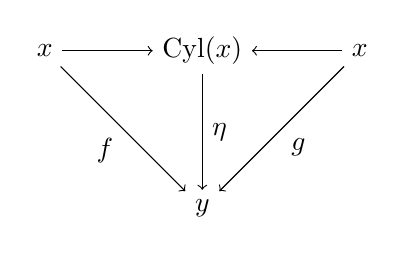
\begin{tikzpicture}
                \node (X) at (-2,0) {$x$};
                \node (X2) at (2,0) {$x$};
                \node (C) at (0,0) {$\mathrm{Cyl}(x)$};
                \node (Y) at (0,-2) {$y$};
                \draw[->] (X) -- (C);
                \draw[->] (X2) -- (C);
                \draw[->] (C) -- node[right]{$\eta$} (Y);
                \draw[->] (X) -- node[below left]{$f$} (Y);
                \draw[->] (X2) -- node[below right]{$g$} (Y);
            \end{tikzpicture}
            \caption{A left homotopy.}
            \label{fig:left_homotopy}
        \end{subfigure}
        \begin{subfigure}[b]{0.49\textwidth}
            \centering
            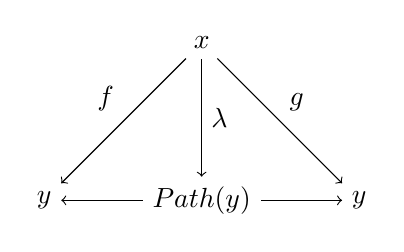
\begin{tikzpicture}
                \node (Y) at (-2,-2) {$y$};
                \node (Y2) at (2,-2) {$y$};
                \node (C) at (0,-2) {$\text{Path}(y)$};
                \node (X) at (0,0) {$x$};
                \draw[<-] (Y) -- (C);
                \draw[<-] (Y2) -- (C);
                \draw[<-] (C) -- node[right]{$\lambda$} (X);
                \draw[<-] (Y) -- node[above left]{$f$} (X);
                \draw[<-] (Y2) -- node[above right]{$g$} (X);
            \end{tikzpicture}
            \caption{A right homotopy.}
            \label{fig:right_homotopy}
        \end{subfigure}
        \caption{Homotopies in a model category.}
    \end{figure}

    \begin{example}[Topological spaces]
        Consider the category $\mathbf{Top}$. A cylinder object for a topological space $X$ is given by the product $X\times[0,1]$. The codiagonal map is factorized as the endpoint inclusion $X\sqcup X\rightrightarrows X\times[0,1]$ followed by the collapse $X\times[0,1]\overset{\pi_X}{\rightarrow}X$, where it is not hard to show that the collapse is a homotopy equivalence. A left homotopy with respect to $X\times[0,1]$ is exactly a homotopy in the sense of \cref{topology:homotopy}.

        A path object $\mathrm{Path}(X)$ is given by the mapping space $X^{[0,1]}$. The diagonal map is factorized by the basepoint inclusion $X\overset{\iota_0}{\rightarrow}X^{[0,1]}$ followed by the endpoint projections $X^{[0,1]}\rightrightarrows X\times X$. That the right homotopies with respect to $X^{[0,1]}$ give the same equivalence classes as the left homotopies is the content of \cref{topology:path_space}.
    \end{example}

    \begin{property}
        If $x$ is cofibrant, every left homotopy induces a right homotopy. Dually, if $y$ is fibrant, every right homotopy induces a left homotopy.
    \end{property}
    \begin{result}[Equivalence relation]
        Whenever $x$ is cofibrant and $y$ is fibrant, the relations of being left-homotopic (or, equivalently, right-homotopic) coincide on $\mathbf{M}(x,y)$ and, in particular, define equivalence relations. The equivalence classes are denoted by $[x,y]$.
    \end{result}

    \begin{property}[Stability under composition]
        Homotopies are preserved under both precomposition and postcomposition by arbitrary morphisms.
    \end{property}
    \begin{property}[Weak equivalences]\label{model:weak_equivalence_homotopy}
        A morphism is a weak equivalence if and only if it is a homotopy inverse.
    \end{property}

    \newdef{Homotopy equivalence}{\index{homotopy!equivalence}
        Two objects in a model category are said to be homotopy equivalent if there exists morphisms $f:x\leftrightarrows y:g$ such that $f\circ g$ and $g\circ f$ are homotopic to the identity. The morphisms $f,g$ are then said to be homotopy equivalences.
    }

    In \cref{model:localization}, it was shown that one can assign to every category with weak equivalences a homotopy category. When the category has the additional structure of a model category, one can construct an equivalent category:
    \newadef{Homotopy category II}{\index{homotopy!category}\label{model:homotopy_category_2}
        The homotopy category $\mathbf{Ho(M)}$ of a model category $\mathbf{M}$ is the category defined by the following data:
        \begin{itemize}
            \item\textbf{Objects}: $\ob{M}$, and
            \item\textbf{Morphisms}: $[x^{\mathrm{cf}},y^{\mathrm{cf}}]$.
        \end{itemize}
    }
    In fact it is easier to restrict to the subcategory $\mathbf{M_{cf}}$ of $\mathbf{Ho(M)}$ on the fibrant-cofibrant objects due to the following property (when restricting to a subcategory, the resulting homotopy category is only equivalent and not isomorphic to the localization):
    \begin{property}
        The homotopy category of a model category is equivalent to those of the full subcategories on (co)fibrant objects:
        \begin{gather}
            \mathbf{Ho(M)}\cong\mathbf{Ho(M_f)}\cong\mathbf{Ho(M_c)}\cong\mathbf{Ho(M_{cf})}.
        \end{gather}
    \end{property}

    The following theorem gives a stronger version of \cref{model:weak_equivalence_homotopy} above:
    \begin{theorem}[Whitehead]\index{Whitehead}
        A weak equivalence between objects that are both fibrant and cofibrant is a homotopy equivalence.
    \end{theorem}

    \begin{property}
        A Quillen equivalence of model categories induces an equivalence of homotopy categories.
    \end{property}

    \begin{property}[Monoidal model categories]
        The homotopy category of a monoidal model category has a closed monoidal structure defined by the induced derived adjunction. The homotopy category of an enriched model category is enriched, powered and copowered over the homotopy category of its enriching category, where the enriched structure is again given by the induced derived adjunction.
    \end{property}

    In some cases it is useful to consider categories that are strictly weaker than model categories but stronger than categories with weak equivalences. The prime example being the full subcategories of a model category on the (co)fibrant objects. These are often easier to handle in the setting of homotopy theory.
    \newdef{Category of fibrant objects}{\index{fibrant object}\index{fibration}
        A category $\mathbf{C}$ with weak equivalences $\mathbf{W}\hookrightarrow\mathbf{C}$ equipped with another subcategory $\mathbf{F}\hookrightarrow\mathbf{C}$ for which the morphisms are called \textbf{fibrations} such that the following conditions are satisfied:
        \begin{enumerate}
            \item $\mathbf{C}$ has finite products.
            \item Fibrations and acyclic fibrations are preserved under arbitrary pullbacks.
            \item Every object admits a good path object.
            \item All objects are fibrant.
        \end{enumerate}
    }

    \begin{theorem}[Factorization lemma]\index{factorization!lemma}
        In a category of fibrant objects any morphism can be factorized as the right inverse of an acyclic fibration followed by a fibration.
    \end{theorem}

    The following theorem is important for characterizing functors that preserve weak equivalences.
    \begin{theorem}[Ken Brown's lemma]\index{Ken Brown}\label{model:ken_brown}
        Let $\mathbf{C}$ be a category of fibrant objects and let $\mathbf{D}$ be a category with weak equivalences. If a functor $\func{F}{C}{D}$ maps acyclic fibrations to weak equivalences, it preserves all weak equivalences.
    \end{theorem}
    \remark{An analogous theorem exists for \textit{categories of cofibrant objects}.}

    The above lemma allows to define derived functors for Quillen functors between model categories (the following definition is also better suited for working in the $\infty$-setting than \cref{model:derived_functor}).
    \newadef{Derived functor}{\index{derived!functor}\label{model:derived_functor_replacement}
        Let $\func{F}{C}{D}$ be a left (resp.~right) Quillen functor. The left (resp.~right) derived functors are obtained by precomposition with the cofibrant (resp.~fibrant) replacement functors.
    }
    \begin{property}[Derived functors are absolute]\label{model:absolute_derived_functors}
        It can be shown that derived functors built using (co)fibrant replacement are given by absolute Kan extensions. So, even though homotopy categories often do not admit all (co)limits, the resulting Kan extensions do exist.
    \end{property}

\subsection{Reedy model structure}

    Consider a bicomplete category $\mathbf{M}$ (this will often be $\mathbf{sSet}$). For any full subcategory inclusion $\mathbf{D}\hookrightarrow\mathbf{C}$ one obtains an induced \textbf{truncation} (or \textbf{restriction}) functor $\tr:\mathbf{M^C}\rightarrow\mathbf{M^D}$. The left and right adjoints of this functor are respectively called the \textbf{skeleton} and \textbf{coskeleton} functors.
    \begin{formula}
        The adjoint functors are defined by Kan extensions and, hence, can be expressed in terms of (co)ends and weighted (co)limits:
        \begin{gather}
            \mathrm{sk}(X)x := \int^{y\in\mathbf{D}}\mathbf{C}(y,x)\cdot Xy = \colim^{\mathbf{C}(-,x)}\\
            \mathrm{cosk}(X)x := \int_{y\in\mathbf{D}}\big[\mathbf{C}(x,y),Xy\big] = \wlim{\mathbf{C}(x,-)}X.
        \end{gather}
    \end{formula}
    \newdef{Skeletal sets}{\index{skeleton}
        Let $\mathbf{M}=\mathbf{sSet}$ and consider the inclusion $\simplex_{\leq n}\hookrightarrow\simplex$ of the full subcategory on the objects $\{[0],\ldots,[n]\}$. The $n$-truncation functor $\tr_n$ discards all simplices of degree higher than $n$ or, in other words, it `truncates' a simplicial set at degree $n$.

        The $n$-skeleton functor $\mathrm{sk}_n$ takes a simplicial set $X$ of degree $\leq n$ and freely adds degenerate simplices in degrees $>n$, i.e.~it is the smallest simplicial set containing $X$ as a simplicial subset. The $n$-coskeleton functor $\mathrm{cosk}_n$ adds a simplex in degree $>n$ whenever all of its faces are present, i.e.~the $m$-simplices in $\text{cosk}_nX$ are given by the collection of all $(m+1)$-tuples of $(m-1)$-simplices that are compatible (along lower simplices).
    }
    \begin{property}[Simplicial nerve]\index{nerve}
        The nerve functor $\func{N}{Cat}{sSet}$ from \cref{model:nerve} is a fully faithful functor to the category of 2-coskeletal simplicial sets. This follows from the fact that in ordinary categories compositions of morphisms are unique and, hence, all higher-order tuples of composable morphisms are determined by composable pairs. In fact, this is just the characterization of (small) categories as categories internal to $\mathbf{Set}$ (under the isomorphism $C_2\cong C_1\times_{C_0}C_1$ which will be called the first \textit{Segal condition} in \cref{model:segal_space}).
    \end{property}

    \newdef{Reedy category}{\index{Reedy category}\label{model:reedy}
        A category $\mathbf{C}$ equipped with a \textbf{degree} function $\ob{C}\rightarrow\alpha$, where $\alpha$ is an ordinal (\cref{set:ordinal}), and two wide subcategories $\mathbf{C}^\pm$ that satisfy the following conditions:
        \begin{enumerate}
            \item Nontrivial morphisms in $\mathbf{C}^+$ (strictly) increase the degree.
            \item Nontrivial morphisms in $\mathbf{C}^-$ (strictly) decrease the degree.
            \item All morphisms admit a unique factorization as a morphism in $\mathbf{C}^-$ followed by a morphism in $\mathbf{C}^+$. This factorization is sometimes called the \textbf{(canonical) Reedy factorization}.
        \end{enumerate}
    }

    \begin{property}[Minimality]\index{degree!of factorization}
        The Reedy factorization is the (unique) factorization of minimal degree, where the \textbf{degree} of a factorization $x\overset{f}{\rightarrow}y\overset{g}{\rightarrow}z$ is defined as the degree of $y$.
    \end{property}
    \begin{property}[Isomorphisms are trivial]
        A morphism in a Reedy category is an isomorphism if and only if it is trivial.
    \end{property}

    \begin{example}
        Some common examples of Reedy categories are discrete categories, finite posets, the simplex category $\simplex$ and opposites of Reedy categories.
    \end{example}

    For Reedy categories one can also define $n$-truncation, $n$-skeleton and $n$-coskeleton functors by restricting to the full subcategories on elements of degree $\leq n$.
    \newdef{Matching and latching objects}{\index{matching!object}\index{latching object}
        Let $\mathbf{R}$ be a Reedy category and consider a diagram $X\in\funccat{R}{C}$ with $\mathbf{C}$ small. Consider the skeleton monad and coskeleton comonad (often just called the skeleton and coskeleton functors) $\mathbf{sk}_n:=\mathrm{sk}_n\circ\tr_n$ and $\mathbf{cosk}_n:=\mathrm{cosk}_n\circ\tr_n$. The latching and matching objects of $X$ are defined as the restrictions of $\mathbf{sk}_{n-1}$ and $\mathbf{cosk}_{n-1}$ to the degree $n$ subcategory of $\mathbf{R}$. The counits of these adjunctions give rise to the \textbf{latching} and \textbf{matching} maps.

        One can also define the latching and matching objects through (co)limits. Define the subcategory $\mathbf{R}^+(r)$ as the subcategory of $\mathbf{R}^+/r$ on all objects except the identity. The latching object $L_rX$ can be shown to be isomorphic to the colimit of $X$ over $\mathbf{R}^+(r)$.
    }

    \begin{example}[Simplicial objects]\index{simplicial!object}\index{Eilenberg--Zilber}
        The above property allows to give a nice interpretation to latching objects in the case of $\mathbf{R}=\simplex^{op}$. Using the \textit{Eilenberg--Zilber lemma} it can be shown that the $n^{th}$ latching object of a simplicial object is given by its collection of degenerate $n$-simplices.
    \end{example}

    \newdef{Boundary}{\index{boundary}
        The boundary $\partial\mathbf{R}(-,r)$ of a representable presheaf $\mathbf{R}(-,r)$ is defined as its latching object. It can be shown that $\partial\mathbf{R}(-,r)$ consists of exactly those morphisms that are not in $\mathbf{R}^-$ or, equivalently, as $\mathbf{sk}_{n-1}\mathbf{R}(-,r)$. The latching map coincides with the canonical inclusion $\partial\mathbf{R}(-,r)\hookrightarrow\mathbf{R}(-,r)$ if $r$ is of degree $n$.
    }
    \begin{formula}
        One can show that the latching and matching objects can be obtained through (co)limits weighted by boundaries:
        \begin{align}
            M_rX &\cong \wlim{\partial\mathbf{R}(r,-)}X\,,\\
            L_rX &\cong \colim^{\partial\mathbf{R}(-,r)}X.\label{model:latching_boundary}
        \end{align}
    \end{formula}

    From here on $\mathbf{M}$ will be assumed to be a model category. In this case a canonical model structure on the functor category $\funccat{R}{M}$ for Reedy $R$ can be defined.
    \newdef{Relative matching and latching objects}{
        Consider the (weighted) colimit bifunctor $\func{\text{colim}}{Psh(R)\times[R,M]}{M}$. The Leibniz construction~\ref{model:pushout_product} allows to define the relative latching object of $f:X\rightarrow Y$ at $r\in\ob{R}$ as the Leibniz product of the boundary inclusion $\partial\mathbf{R}(-,r)\hookrightarrow\mathbf{R}(-,r)$ and $f$.

        By \namecrefs{cat:weighted_hom_colimit}~\eqref{cat:weighted_hom_colimit} and~\eqref{model:latching_boundary}, the relative latching map is of the form $Xr\sqcup_{L_rX}L_rY\rightarrow Yr$ and the relative matching map is of the form $Xr\rightarrow Yr\times_{M_rY}M_rX$.
    }

    \begin{property}[Reedy model structure]
        Let $\mathbf{R}$ be a Reedy category and let $\mathbf{M}$ be a model category. The functor category $\funccat{R}{M}$ admits the following model structure:
        \begin{itemize}
            \item\textbf{Weak equivalences}: the objectwise weak equivalences.
            \item\textbf{Fibrations}: morphisms for which the relative matching map is a fibration (in $\mathbf{M}$) for all $r\in\ob{R}$
            \item\textbf{Cofibrations}: morphisms for which the relative latching map is a cofibration (in $\mathbf{M}$) for all $r\in\ob{R}$
        \end{itemize}
    \end{property}

    \begin{property}[Quillen (co)limit functors]
        Consider a $\mathcal{V}$-enriched model category $\mathbf{M}$ and a Reedy category $\mathbf{R}$. For every Reedy cofibrant functor $W$ in $\funccat{R}{\mathcal{V}}$, the weighted limit and colimit functors are right and left Quillen, respectively.
    \end{property}

    ?? COMPLETE (this section is too abstract and difficult at this point) ??

\section{Simplicial spaces}
\subsection{Kan complexes}

    \newdef{Horn}{\index{horn}
        Consider the standard simplex $\Delta[n]$. For all $n\geq1$ and $0\leq k\leq n$ the $(n,k)$-horn $\Lambda^k[n]$ is defined as the subsimplicial set obtained by removing the $k^{th}$ face from $\partial\Delta[n]$. When $k=0$ or $k=n$, the horn is said to be \textbf{outer}, otherwise it is said to be \textbf{inner}.
    }

    \newdef{Kan fibration}{\index{Kan!fibration}
        A morphism of simplicial sets that has the right lifting property with respect to all horn inclusions $\Lambda^k[n]\hookrightarrow\Delta[n]$.
    }
    \newdef{Kan complex}{\index{Kan!complex}\label{model:kan_complex}
        \nomenclature[S_Kan]{$\mathbf{Kan}$}{category of Kan complexes}
        A simplicial set that has all horn fillers or, equivalently, a simplicial set for which the terminal morphism is a Kan fibration. The full subcategory of $\mathbf{sSet}$ on Kan complexes is denoted by $\mathbf{Kan}$.
    }

    \begin{property}[Horn filler condition]\label{model:horn_filler}
        A simplicial set is the nerve of a (small) category if and only if all of its inner horns admit a unique filler (compositions are unique). If one requires all horns to admit a unique filler, the nerve of a groupoid is obtained.
    \end{property}

    By relaxing the above requirements one can generalize the notion of a category (this is due to \textit{Boardman} and \textit{Vogt}).
    \newdef{Quasicategory\footnotemark}{\index{quasi-!category}\index{logos}\index{Boardman condition}\label{model:quasicategory}
        \footnotetext{Some authors such as \textit{Joyal} call these \textbf{logoi} (singular: \textbf{logos}).}
        A simplicial set for which all inner horns have (not necessarily unique) fillers. This condition is sometimes called the \textbf{Boardman condition}.
    }

    At this point a third instance of a `homotopy category' can be defined.
    \newdef{Homotopy category III}{\index{homotopy!category}
        Let $X$ be a quasicategory. The homotopy category $\mathbf{Ho}(X)$ consists of the following data:
        \begin{itemize}
            \item\textbf{Objects}: $X_0$, and
            \item\textbf{Morphisms}: The quotient of $X_1$ under the relation $f\circ g\sim h$ if there exists a 2-simplex with edges $f,g$ and $h$.
        \end{itemize}
    }
    \begin{property}[Fundamental category]\index{fundamental!category}
        If $X$ is a quasicategory, its homotopy category is equivalent to its \textbf{fundamental category} $\pi_1(X)$, i.e.~the image under the left adjoint of the (simplicial) nerve functor.
    \end{property}

    The following theorem is a restatement of \cref{model:horn_filler}.
    \begin{theorem}[Joyal]\index{Joyal}
        A quasicategory is a Kan complex if and only if its homotopy category is a groupoid.
    \end{theorem}

\subsection{Simplicial localization}

    \newdef{Homotopy category IV}{\index{homotopy!category}\label{model:enriched_homotopy_category}
        Consider a simplicially enriched category $\mathbf{C}$. Its homotopy category $\pi_0(\mathbf{C})$ is defined as follows:
        \begin{itemize}
            \item\textbf{Objects}: $\ob{C}$, and
            \item\textbf{Morphisms}: $\pi_0\mathbf{C}(x,y)$.
        \end{itemize}
        Two morphism $f,g\in\mathbf{C}(x,y)$ are said to be \textbf{homotopic} if they are identified in $\pi_0(\mathbf{C})$. A morphism $f\in\mathbf{C}(x,y)$ is called a \textbf{homotopy equivalence} if it admits both a left and a right inverse in $\pi_0(\mathbf{C})$, i.e.~if it becomes an isomorphism in the homotopy category.
    }
    \newdef{Dwyer--Kan equivalence I}{\index{equivalence!Dwyer--Kan}\label{model:enriched_dwyer_kan}
        Consider a simplicial functor $\func{F}{C}{D}$ between two simplicially enriched categories. This functor is called a Dwyer--Kan equivalence if:
        \begin{itemize}
            \item $F$ is \textbf{$\infty$-fully faithful}, i.e.~the induced map on hom-objects is a weak equivalence.\footnote{This is a generalization of the ordinary definition for categories. (Simplicial categories will give models for \textit{$\infty$-categories.})}
            \item The induced map on connected components $\pi_0( F):\pi_0(\mathbf{C})\rightarrow\pi_0(\mathbf{D})$ is an equivalence (of categories). In fact, this condition can be relaxed to $\pi_0(F)$ being essentially surjective, since together with the previous condition this implies that $\pi_0(F)$ is an equivalence.
        \end{itemize}
    }

    \begin{construct}[Hammock localization]\index{localization!hammock}\index{simplicial!localization}
        Let $(\mathbf{C},W)$ be a category with weak equivalences. Its hammock localization (or \textbf{simplicial localization}) $L^H\mathbf{C}$ is the simplicially enriched category constructed as follows:
        \begin{itemize}
            \item\textbf{Objects}: $\ob{C}$, and
            \item\textbf{Morphisms}: $L^H\mathbf{C}(x,y)$ is the simplicial set defined as follows:
            \begin{quote}
                First, for every $n\in\mathbb{N}$ one constructs a category with as objects the zigzags of morphisms in $\mathbf{C}$ relating $x$ and $y$ such that all left-pointing morphisms are in $W$, and as morphisms the endpoint-preserving `natural transformations' (in the sense that all triangles/squares in the resulting diagram commute). Then, the coproduct is taken over the (simplicial) nerves of the categories for all $n\in\mathbb{N}$. Finally, the quotient is taken by the equivalence relations generated by:
                \begin{enumerate}
                    \item inserting or removing identity morphisms, and
                    \item composing morphisms.
                \end{enumerate}
            \end{quote}
        \end{itemize}
    \end{construct}

    The following property relates all constructions of what could be called homotopy categories.
    \begin{property}
        Let $(\mathbf{C},W)$ be a category with weak equivalences. It can be shown that
        \begin{gather}
            \mathrm{Ho}(L^H\mathbf{C})\cong\mathbf{C}[W^{-1}].
        \end{gather}
        This construction gives a more explicit description of the homotopy category. Furthermore, if $\mathbf{M}$ is a simplicial model category, the categories $\mathbf{M_{cf}}$ and $L^H\mathbf{M}$ are Dwyer--Kan equivalent.
    \end{property}
    \begin{property}
        Quillen equivalent model categories have Dwyer--Kan equivalent simplicial localizations.
    \end{property}
    \begin{property}
        Up to Dwyer--Kan equivalence, every simplicially enriched category can be obtained as the simplicial localization of a category with weak equivalences.
    \end{property}

    \newdef{Simplicial resolution}{\index{resolution!(co)simplicial}
        Consider an object $x$ in a model category $\mathbf{M}$. A (co)simplicial resolution of $x$ is a Reedy (co)fibrant (co)simplicial object $X$ together with a weak equivalence $x\simeq X_0$.

        Every object in a model category admits a (co)simplicial resolution by taking a (co)fibrant replacement of the constant (co)simplicial object.
    }

    \newdef{Bergner model structure}{\index{Bergner model structure}
        The catgory of simplicially enriched categories admits the following model structure:
        \begin{itemize}
            \item\textbf{Weak equivalences}: Dwyer--Kan equivalences,
            \item\textbf{Cofibrant objects}: \textit{simplicial computads}, and
            \item\textbf{Fibrant objects}: $\mathbf{Kan}$-enriched categories.
        \end{itemize}
    }
    \newconstr{Free resolution}{\index{resolution}\label{model:bergner_free_resolution}
        Consider a (small) category $\mathbf{C}$. From this category we can construct a simplicial category $\mathfrak{C}\mathbf{C}$ consisting of the following data:
        \begin{itemize}
            \item\textbf{Objects}: $\ob{C}$, and
            \item\textbf{Morphisms}: $\mathrm{hom}(\mathfrak{C}\mathbf{C})_n := \mathrm{hom}(F^{n+1}\mathbf{C})$, where $F$ is identity-on-objects and $F\mathbf{C}$ has as morphisms strings of composable morphisms in $\mathbf{C}$.
        \end{itemize}
        It can be shown that $\mathfrak{C}\mathbf{C}$ is a \textit{simplicial computad} for any simplicially enriched category $\mathbf{C}$, $\mathfrak{C}$ acts as the cofibrant replacement functor in the Bergner model structure.
    }

\subsection{Segal spaces}

    \begin{example}[Bisimplicial sets]
        One can also look at simplicial objects in $\mathbf{sSet}$ (these are in particular $\mathbf{sSet}$-enriched). Such objects are often called bisimplicial sets or \textbf{simplicial spaces}\footnote{The latter name follows from the fact that topological spaces and simplicial sets are (Quillen-)equivalent.}. Since $\mathbf{sSet}$ is a model category, \cref{model:model_functor_category} above says that $\mathbf{ssSet}$ itself admits a model structure. It can furthermore be shown that the injective model structure on $\mathbf{ssSet}$ coincides with the Reedy model structure (a rather nontrivial statement).
    \end{example}

    \newdef{Segal space}{\index{Segal!space}\index{spine}\label{model:segal_space}
        Consider a fibrant object $X$ in the injective (or Reedy) model structure on $\mathbf{ssSet}$. This bisimplicial set is called a Segal space if it satisfies the following weak form of the \textit{Segal condition} for all $n\geq1$:\footnote{If the Reedy condition is omitted, the limit on the right-hand side has to be replaced by a \textit{homotopy limit}.}
        \begin{gather}
            X_n\simeq X_1\times_{X_0}\cdots\times_{X_0}X_1\ \ (n\text{ factors}).
        \end{gather}
        These maps are called \textbf{Segal maps} (even when they are not weak equivalences). They are the morphisms induced by \textbf{spine} inclusions, i.e.~inclusions of the union of edge 1-cells.
    }
    \newdef{Segal category}{\index{Segal!category}
        A bisimplicial set $X$ is called a \textbf{Segal precategory} if $X_0$ is discrete. It is called a Segal category if in addition all its Segal maps are weak equivalences, i.e.~if it is a Segal space with a discrete set of `objects'.
    }

    \newdef{Mapping space}{\index{mapping!space}
        Consider a Segal space $X$. For every two points $x,y\in X_0$, the mapping space $\mathrm{Map}(x,y)$ is defined as the fibre of $(d_1,d_0):X_1\rightrightarrows X_0\times X_0$ over the point $(x,y)$. The identity element for $x\in X_0$ is given by $s_0(x)$.
    }

    The following two definitions should be compared to \namecrefs{model:enriched_homotopy_category}~\ref{model:enriched_homotopy_category} and~\ref{model:enriched_dwyer_kan}.
    \newdef{Homotopy category V}{\index{homotopy!category}
        Consider a Segal category $X$. Its homotopy category $\mathbf{Ho}(X)$ is defined as follows:
        \begin{itemize}
            \item\textbf{Objects}: $X_0$, and
            \item\textbf{Morphisms}: $\pi_0\mathrm{Map}(x,y)$.
        \end{itemize}
        Two points $f,g\in\mathrm{Map}(x,y)$ are said to be \textbf{homotopic} if they are identified in $\mathbf{Ho}(X)$. A point $f\in\mathrm{Map}(x,y)$ is called a \textbf{homotopy equivalence} if it admits both a left and a right inverse in $\mathbf{Ho}(X)$, i.e.~if it becomes an isomorphism. The subspace $X_\mathrm{hoequiv}\subset X_1$ consists of the components that contain homotopy equivalences.\footnote{It should be noted that if any point in a component is a homotopy equivalence, all points in that component are homotopy equivalences.}
    }
    \newdef{Dwyer--Kan equivalence II}{\index{equivalence!Dwyer--Kan}
        A map $F$ of Segal spaces such that:
        \begin{enumerate}
            \item the induced map on mapping spaces is a weak equivalence.
            \item the induced map between homotopy categories is an equivalence (of categories).
        \end{enumerate}
    }

    \newdef{Complete Segal space}{
        A Segal space $X$ for which the map $s_0:X_0\rightarrow X_\mathrm{hoequiv}$ is a weak equivalence.
    }
    \begin{property}[Dwyer-Kan equivalence]
        A map of Segal spaces is a Dwyer--Kan equivalence if and only if it is a weak equivalence in the \textit{complete Segal space model structure}. A map of complete Segal spaces is a Dwyer--Kan equivalence if and only if it is a levelwise weak equivalence.
    \end{property}

\subsection{Coherent nerve}

    The nerve and realization functors (\cref{model:nerve_and_realization}) can also be modified to incorporate the higher homotopical data present in a simplicially enriched category.

    First, define a cosimplicial simplicially enriched category $\func{C}{\Delta}{sSetCat}$ that assigns to every finite ordinal $[n]$ the category consisting of the following data:
    \begin{itemize}
        \item\textbf{Objects}: $[n]\equiv\{0,1,\ldots,n\}$
        \item\textbf{Morphisms}: $C[n](i,j) := N(P_{ij})$, where $N$ is the ordinary nerve functor on $\mathbf{Cat}$ and $P_{ij}$ is the poset consisting of all subsets of $\{i,\ldots,j\}$ that contain both $i$ and $j$.
    \end{itemize}
    The (homotopy) \textbf{coherent nerve functor} (or \textbf{simplicial nerve functor}\footnote{This terminology was also used for the ordinary nerve functor taking values in $\mathbf{sSet}$. In general it should be clear from the context which one is meant.}) is the nerve functor induced by this cosimplicial object. It not only knowns about all possible morphisms, it also knows about all possible ways how one can obtain this morphism.
    \begin{remark}
        The cosimplicial object $\func{C}{\Delta}{sSetCat}$ is in fact just the free resolution functor $\mathfrak{C}$ in the Bergner model structure (\cref{model:bergner_free_resolution}) restricted to the subcategory $\simplex$.
    \end{remark}

    \begin{property}
        The homotopy coherent nerve functor $N_\Delta$ is uniquely determined by the following relation:
        \begin{gather}
            \mathbf{sSet}(\Delta[n],N_\Delta\mathbf{C})=\mathbf{sSetCat}(C[n],\mathbf{C})\,.
        \end{gather}
    \end{property}

    \begin{property}[Simplicial realization]
        The left adjoint of the homotopy coherent nerve functor satisfies the following relation for all finite ordinals $[n]$:
        \begin{gather}
            |\Delta[n]|\cong C[n]\,.
        \end{gather}
    \end{property}

    \begin{property}[Quasicategories]
        If $\mathbf{C}$ is $\mathbf{Kan}$-enriched, its coherent nerve is a quasicategory. By \cref{model:simplicial_model_category} this allows to associate a quasicategory to any simplicial model category by passing to the coherent nerve of its fibrant-cofibrant subcategory.
    \end{property}

    At this point it is interesting to reconsider the simplicial nerve construction (\cref{model:nerve}). Although the functor $\func{N}{Cat}{sSet}$ is fully faithfull, there is a problem in that weak equivalences of simplicial sets do not necessarily correspond to (weak) equivalences of categories. The issue comes from the definition of the canonical model structure (\cref{model:sset_model_structure}) on $\mathbf{sSet}$. Here, the weak equivalences are those morphisms that become weak equivalences after geometric realization. During this step information about the direction of morphisms is lost and it becomes impossible to distinguish categories from groupoids. Only when all morphisms are assumed to be invertible, i.e.~the category is assumed to be groupoid, does one recover the converse statement.

    A first solution is to use a different model structure with less weak equivalences.
    \newdef{Joyal model structure}{\index{Joyal!model structure}
        The category $\mathbf{sSet}$ of simplicial sets (\cref{model:simplicial set}) admits a model structure defined by the following data:
        \begin{itemize}
            \item\textbf{Weak equivalences}: \textit{weak categorical equivalences}, i.e.~maps $f:X\rightarrow Y$ such that the induced simplicial functor $C(f):C(X)\rightarrow C(Y)$ is a Dwyer-Kan equivalence.
            \item\textbf{Cofibrations}: monomorphisms.
            \item\textbf{Fibrant objects}: quasicategories (\cref{model:quasicategory}).
        \end{itemize}
    }
    When characterizing those simplicial sets that are nerves of categories, groupoids and categories are distinguished by whether all horns admit a (unique) filler or only inner horns admit a (unique) filler. However, when the fibrant objects are Kan complexes (those simplicial sets that admit all horn fillers), the homotopical structure only knows about nerves that come from a groupoid. By passing to the larger class of quasicategories, this problem is solved.

    Instead of changing the model structure on $\mathbf{sSet}$ to overcome the issues with taking nerves of categories or groupoids, one can also change the construction of the nerve functor. An alternative approach was introduced by \textit{Rezk}.
    \newdef{Classifying diagram}{\index{classifying!diagram}
        Consider a (small) category $\mathbf{C}$ together with the functor category $\mathbf{C}^{[n]}$ where $[n]$ is the totally ordered set on $n+1$ elements. The classifying diagram of $\mathbf{C}$ is the bisimplicial set $\widetilde{N}\mathbf{C}$ defined levelwise as follows:
        \begin{gather}
            \widetilde{N}\mathbf{C}_k := N(\mathrm{Core}(\mathbf{C}))\,,
        \end{gather}
        where $N$ is the ordinary nerve functor and $\mathrm{Core}$ denotes the core functor (\cref{cat:core}).

        The reason for why this construction is better for distinguishing categories and groupoids comes from the fact that information about isomorphisms is already captured at degree 0, while information about noninvertible morphisms is only captured from degree 1 onwards.
    }
    \begin{property}
        If $\mathbf{C}$ is small, then $\widetilde{N}\mathbf{C}$ is a complete Segal space.
    \end{property}

    ?? COMPLETE ??

\section{Cofibrantly generated categories}
\subsection{Transfinite constructions}

    Before proceeding, some notions from ordinary category need to be specialized to the context of regular cardinals (\cref{set:regular_cardinal}). In this section the symbol $\kappa$ will always denote such a regular cardinal.

    \newdef{$\kappa$-filtered category}{\index{category!filtered}
        A category in which every diagram with less than $\kappa$ arrows admits a cocone.
    }
    \newdef{$\kappa$-directed limit}{\index{limit!directed}
        Consider a poset $I$ such that every subposet of cardinality less than $\kappa$ has a lower bound (upper bound for directed colimits). Such a set is said to be $\kappa$-(co)directed. A limit of a diagram over this poset is called a $\kappa$-(co)directed (co)limit.
    }
    The following definition is a categorification of the previous one:
    \newdef{$\kappa$-filtered limit}{\index{limit!filtered}
        Consider a diagram $\func{D}{I}{C}$. The limit (resp.~colimit) of $D$ is said to be $\kappa$-cofiltered (resp.~$\kappa$-filtered) if $\mathbf{I}$ is a $\kappa$-cofiltered (resp.~$\kappa$-filtered) category.

        It should be noted that an analogue of \cref{cat:directed_filtered} also holds in the $\kappa$-context, i.e.~a category has all $\kappa$-directed limits if and only if it has all $\kappa$-filtered limits (and analogously for colimits).
    }

    \newdef{Small object}{\index{small}\index{presentable}
        An object for which there exists a regular cardinal $\kappa$ such that its covariant hom-functor preserves all $\kappa$-filtered colimits. These objects are also said to be \textbf{$\kappa$-compact} or \textbf{$\kappa$-presentable}.
    }
    \newdef{Accessible category}{\index{accessible}
        A locally small category $\mathbf{C}$ for which there exists a regular cardinal $\kappa$ such that $\mathbf{C}$ has all $\kappa$-filtered colimits and such that it is generated under $\kappa$-filtered colimits by a small subcategory $\mathbf{D}$ of $\kappa$-small objects, i.e.~$\mathbf{C}\cong\mathrm{Ind}_\kappa(\mathbf{D})$.
    }
    \newdef{Locally presentable category}{\index{presentable}
        A cocomplete, accessible category. It can be shown that such categories are also complete and, hence, bicomplete.
    }

    \begin{property}
        Every locally presentable category can be obtained as a full reflective subcategory of a presheaf category under an \textbf{accessible embedding}, i.e.~an embedding that preserves filtered colimits.
    \end{property}
    \begin{property}[Gabriel-Ulmer duality]\index{Gabriel-Ulmer duality}
        First, define the following two 2-categories. $\mathbf{LFP}$ consists of the following data:
        \begin{itemize}
            \item\textbf{Objects}: locally finitely presentable categories,
            \item\textbf{1-Morphisms}: right adjoint functors preserving filtered colimits, and
            \item\textbf{2-Morphisms}: natural transformations.
        \end{itemize}
        $\mathbf{Lex}$ consists of the following data:
        \begin{itemize}
            \item\textbf{Objects}: small, finitely complete categories,
            \item\textbf{1-Morphisms}: left exact functors, and
            \item\textbf{2-Morphisms}: natural transformations.
        \end{itemize}
        There exists an equivalence $\mathbf{Lex}^{op}\cong\mathbf{LPF}$ that sends a small, finitely complete category to its category of left exact copresheaves.
    \end{property}

    \begin{theorem}[Adjoint functor theorem\footnotemark]\index{adjoint functor theorem}
        Consider a functor $\func{F}{C}{D}$ between locally presentable categories. $F$ admits a right adjoint if and only if it preserves all colimits. $F$ admits a left adjoint if and only if it is accessible and if it preserves all limits.
    \end{theorem}

    For ordinary categories the axioms guarantee the existence of a (unique) composition of any finite number of (composable) morphisms. However, in some cases it is useful, or even necessary, to talk about the `composite' of an infinite number of morphisms:
    \newdef{Transfinite composition}{\index{composition}\index{continuous}\label{cat:transfinite_composition}
        Consider a category $\mathbf{C}$ with a collection of morphisms $I\subseteq\mathrm{hom}(\mathbf{C})$ and let $\alpha$ be an infinite ordinal. An $\alpha$-indexed \textbf{transfinite sequence} of morphisms in $I$ is a diagram of the form $\func{D}{\alpha}{C}$ such that:
        \begin{enumerate}
            \item Successor morphisms in $\alpha$ are mapped to elements of $I$.
            \item $D$ is `continuous' in the sense that for every limit ordinal $\beta<\alpha$: $D\beta\cong\underset{\gamma<\beta}{\colim}\ D\gamma$.
        \end{enumerate}
        $D\lambda$ denotes the restriction of $D$ to the (full) subdiagram $\{\gamma\mid\gamma<\lambda\}$ of $\alpha$. The transfinite composition of this sequence is the induced morphism $D_0\rightarrow D\alpha\equiv\colim\ D$.
    }
    \newdef{Cell complex}{\index{cell!complex}
        Consider a cocomplete category $\mathbf{C}$ with a collection of morphisms $I\subseteq\mathrm{hom}(\mathbf{C})$. A \textbf{relative} $I$-cell complex is a transfinite composition of pushouts (of coproducts\footnote{It can be shown that closure under coproducts follows automatically.}) of morphisms in $I$. An $I$-cell complex is an object such that the unique morphism from the initial object is a relative $I$-cell complex.
    }
    \newnot{Relative cell complexes}{
        The set of all relative $I$-cell complexes is often denoted by $\mathrm{cell}(I)$.
    }

\subsection{Cofibrant generation}

    The following is a famous result by \textit{Quillen}:
    \begin{theorem}[Small object argument]\index{small!object argument}
        Let $\mathbf{C}$ be a locally presentable category with a collection of morphisms $I\subseteq\mathrm{hom}(\mathbf{C})$. Every morphism in $\mathbf{C}$ can be factorized as the composition of a morphism in $\mathrm{rlp}(I)$ followed by a morphism in $\mathrm{cell}(I)$.
    \end{theorem}
    \begin{remark}
        This theorem can be generalized to cocomplete categories where the morphisms in $I$ are small relative\footnote{\textit{Small relative to a set of morphisms} is defined just as ordinary smallness, but with general $\kappa$-filtered colimits replaced by those that start from morphisms in the given set.} to $\mathrm{cell}(I)$. Sets of morphisms with this property are said to \textbf{admit a small object argument}.
    \end{remark}

    \newdef{Cofibrantly generated model category}{\index{model!category}
        Consider a model category $\mathbf{C}$. This category is said to be cofibrantly generated by two sets of morphisms $I,J\subseteq\mathrm{hom}(\mathbf{C})$ if it satisfies the following conditions:
        \begin{enumerate}
            \item $I$ and $J$ both admit the small object argument.
            \item The fibrations are given by $\mathrm{rlp}(J)$.
            \item The acyclic fibrations are given by $\mathrm{rlp}(I)$.
        \end{enumerate}
        It can be shown that the last two conditions are equivalent to the following ones:
        \begin{enumerate}
            \item[$2^*.$] The cofibrations are the retracts (in the arrow category) of $\mathrm{cell}(I)$.
            \item[$3^*.$] The acyclic cofibrations are the retracts (in the arrow category) of $\mathrm{cell}(J)$.
        \end{enumerate}
        The morphisms in $I$ and $J$ are called the \textbf{generating cofibrations} and \textbf{generating acyclic cofibrations}, respectively.
    }

    Sometimes it is desirable to replace the model structure on a category $\mathbf{C}$ by one that has more weak equivalences (denote the new one by $\mathbf{C}_0$). If the cofibrations remain the same, this new structure has some nice properties.
    \begin{itemize}
        \item The fibrations are a subclass of the original ones.
        \item The acyclic fibrations remain the same.
        \item The identity functors $\mathbbm{1}_{\mathbf{C}_0}:\mathbf{C}_0\leftrightarrows\mathbf{C}:\mathbbm{1}_\mathbf{C}$ form a Quillen adjunction.
        \item Every object in $\mathbf{C}$ is weakly equivalent (in $\mathbf{C}_0$) to one in $\mathbf{C}_0$.
    \end{itemize}

    This procedure can be made explicit for a specific class of model categories. Let $\mathbf{C}$ be a left proper, cofibrantly generated, simplicial model category and consider a collection $S\subset\mathrm{hom}(\mathbf{C})$ of cofibrations with cofibrant domain. First, the notion of `$S$-local objects' is introduced.
    \newdef{Local object}{\index{local!object}
        A fibrant object $x$ is said to be $S$-local if for all morphisms in $S$ the image under the Yoneda embedding of $x$ is an acyclic Kan fibration. Analogously, a morphism is called an $S$-local weak equivalence if for all $S$-local fibrant objects its image under their Yoneda embeddings is an acyclic Kan fibration.
    }
    \begin{property}
        Every weak equivalence is an $S$-local weak equivalence: $W\subset W_S$.
    \end{property}

    \begin{construct}[Left Bousfield localization]\index{localization!Bousfield}
        Given a model category $\mathbf{C}$ with the same assumptions as before, the (left) Bousfield localization $L_S\mathbf{C}$ is defined as as the same category but with the following model structure:
        \begin{itemize}
            \item\textbf{Cofibrations}: $\mathrm{cof}(\mathbf{C})$, and
            \item\textbf{Acyclic cofibrations}: cofibrations that are $S$-local weak equivalences.
        \end{itemize}
        If it exists, the Bousfield localization $L_S\mathbf{M}$ of $\mathbf{M}$ at $S$ is the universal left Quillen functor $\gamma:\mathbf{M}\rightarrow L_S\mathbf{M}$ such that its left derived functor sends the image of $S$ to isomorphisms in $\mathbf{Ho}(\mathbf{M})$. The identity functor gives a Quillen adjunction between $\mathbf{M}$ and $L_S\mathbf{M}$ and the induced adjunction on homotopy categories defines a reflective localization.
    \end{construct}
    \begin{remark}
        The notions of local object/morphisms can be slightly generalized (they give equivalent localizations). An \textbf{$S$-local morphism} $f:a\rightarrow b$ is a morphism such that for all objects $x\in\ob{M}$ for which the map
        \begin{gather}
            \mathbf{M}(g^{\mathrm{c}},x^{\mathrm{f}}):\mathbf{M}(d^{\mathrm{c}},x^{\mathrm{f}})\rightarrow\mathbf{M}(c^{\mathrm{c}},x^{\mathrm{f}})
        \end{gather}
        is a weak equivalence for all $g\in S$ ($x$ is said to be \textbf{$S$-local}), the map
        \begin{gather}
            \mathbf{M}(f^{\mathrm{c}},x^{\mathrm{f}}):\mathbf{M}(b^{\mathrm{c}},x^{\mathrm{f}})\rightarrow\mathbf{M}(a^{\mathrm{c}},x^{\mathrm{f}})
        \end{gather}
        is also a weak equivalence. This is the homotopical version of \cref{cat:local_object}, after cofibrant (resp.~fibrant) replacement of the domain (resp.~codomain), the Yoneda embedding of every $S$-local object is weak equivalence, where $S$-local objects are those objects whose Yoneda embedding maps morphisms in $S$ to weak equivalences.
    \end{remark}

    \newdef{Combinatorial model category}{
        A locally presentable, cofibrantly generated model category.
    }

    \begin{theorem}[Dugger]\index{Dugger}\label{model:dugger}
        Every combinatorial model category is Quillen equivalent to a (left) Bousfield localization of a category of simplicial presheaves on a small category (with the global projective model structure).
    \end{theorem}

    ?? FINISH ??

\section{Homotopy (co)limits}

    Consider a category $\mathbf{C}$ with weak equivalences together with diagrams $\func{D,D'}{I}{C}$. Assume that there exists a weak equivalence between $D$ and $D'$, i.e.~a natural transformation that consists of componentwise weak equivalences. Clearly this induces a morphism between (co)limits, but it would be nice if the construction of (co)limits would also preserve the homotopical structure, i.e.~weakly equivalent diagrams should have weakly equivalent (co)limits.

    The main purpose of this section is to introduce a modification of the ordinary (co)limit functors that takes into account the homotopical structure of the underlying categories. A first step is the modification of (co)products:
    \newdef{Homotopy (co)products}{\index{homotopy!(co)product}
        In ordinary categories the universal property of a product (and dually for coproducts) characterizes it as an object with an isomorphism
        \begin{gather}
            \mathbf{C}(-,c)\cong\prod_{i\in I}\mathbf{C}(-,c_i)
        \end{gather}
        such that every $I$-indexed collection of morphisms $f_i:x\rightarrow c_i$ can be factorized as follows
        \begin{gather*}
            \begin{tikzpicture}
                \node (X) at (-1, 1) {$x$};
                \node (C) at (-1, -1) {$c$};
                \node (CI) at (1, -1) {$c_i\,.$};
                \draw[->] (X) -- node[above right]{$f_i$} (CI);
                \draw[->] (C) -- node[below]{$\pi_i$} (CI);
                \draw[->, dashed] (X) -- node[left]{$\exists!$} (C);
            \end{tikzpicture}
        \end{gather*}
        To obtain a homotopical version, the commutativity of this diagram is relaxed up to a homotopy/path in $\mathbf{M}(x,c_i)$. This leads to the definition of a homotopy product as an object $c$ together with a natural weak (homotopy) equivalence
        \begin{gather}
            \psi_x:\mathbf{C}(x,c)\simeq\prod_{i\in I}\mathbf{C}(x,c_i)\,.
        \end{gather}
        The homotopy (co)products are unusual in the sense that they can be obtained as (co)limits in the homotopy category $\mathbf{Ho(C)}$.
    }

    More generally, one can define homotopy (co)limits in any homotopical category by passing to derived functors.
    \newdef{Homotopy (co)limits}{\index{homotopy!(co)limits}
        Let $\mathbf{A}$ be a homotopical category and let $\mathbf{B}$ be a small category. The homotopy limit and colimit functors are defined as the derived functors of the limit and colimit functors $\mathrm{(co)lim}:\funccat{B}{A}\rightarrow\mathbf{A}$.
    }
    \begin{remark}
        The reason for why (co)products can be obtained as ordinary (co)limits  is related to the fact that their indexing categories are discrete. In this case the adjoint of the derived functor is equivalent to the diagonal functor on the homotopy category.
    \end{remark}

    \begin{property}[Model categories]
        Consider the specific case where $\mathbf{C}$ is a model category. If $\funccat{D}{C}$ admits an injective (resp.~projective) model structure, the homotopy limit (resp.~colimit) always exists and can be obtained through fibrant (resp.~cofibrant) replacement as in \cref{model:derived_functor_replacement}.
    \end{property}
    \begin{example}[Reedy categories]
        Consider the general case of diagrams $\func{D}{R}{C}$ with $\mathbf{R}$ Reedy. First, note that the constant functor $\func{\Delta}{C}{[R,C]}$ maps weak equivalences to (pointwise) weak equivalences.\footnote{This is also true when $\mathbf{R}$ is not Reedy.} If the Reedy structure is such that the constant functor preserves cofibrations, then this functor is left-Quillen and Ken Brown's lemma~\ref{model:ken_brown} implies that its right Quillen adjoint, the limit functor, preserves weak equivalences. In this case one can define the \textbf{homotopy limit} $\mathrm{holim}\,D$ as the functor $\lim(D\circ Q_\mathrm{f})$, where $Q_\mathrm{f}$ is the fibrant replacement-functor (which in this case acts pointwise). A dual construction gives rise to \textbf{homotopy colimits}.
    \end{example}

\subsection{Simplicially enriched diagrams}

    In the setting where diagrams are enriched over $\mathbf{sSet}$, one can define homotopy (co)limits in a more sophisticated way.

    \newdef{Homotopy colimit}{
        Consider a diagram $\func{D}{I}{C}$ with $\mathbf{C}$ copowered over $\mathbf{sSet}$. The homotopy colimit of $D$ is defined as the following tensor product (\cref{cat:copower_product}):
        \begin{gather}
            \mathrm{hocolim}\,D := N(-/\mathbf{I})\otimes_\mathbf{I}D = \int^{i\in\mathbf{I}}N(i/\mathbf{I})\cdot Di\,,
        \end{gather}
        where $N$ is the nerve functor (\cref{model:nerve}).
    }
    A similar definition for homotopy limits can be used when the category is powered over $\mathbf{sSet}$:
    \newdef{Homotopy limit}{
        Consider a diagram $\func{D}{I}{C}$ with $\mathbf{C}$ powered over $\mathbf{sSet}$. The homotopy limit of $D$ is defined as the following hom-like object:
        \begin{gather}
            \mathrm{holim}\,D := \int_{i\in\mathbf{I}}[N(\mathbf{I}/i),Di]\,.
        \end{gather}
        This is exactly the characterization of the homotopy limit as the $\mathbf{sSet}$-natural transformations between $N(\mathbf{I}/-)$ and $D$.
    }
    \begin{remark}[Bousfield--Kan map]\index{Bousfield--Kan map}
        The expressions from the above formulas are also known as the \textbf{Bousfield--Kan formulas}. It should be noted that the above definitions are not strictly equivalent to the ones from the previous section. To be precise, the Bousfield--Kan formulas are only weakly equivalent to the general definitions if the objects in $\mathbf{C}$ are replaced by their (co)fibrant replacements, i.e.~if in the above expressions $D$ is postcomposed by a (co)fibrant replacement functor.
    \end{remark}

    ?? COMPLETE (CHECK THESE STATEMENTS) ??

    By \cref{model:homotopy_category_2} one can construct morphisms in a homotopy category as morphisms from a cofibrant replacement to a fibrant replacement. This allows to define diagrams-up-to-homotopy (in two settings).
    \newdef{Homotopy coherent diagram}{\index{homotopy!diagram}
        A morphism in the homotopy category of the Bergner model category. When considering diagrams taking values in a $\mathbf{Kan}$-enriched category, one can use the free resolution functor to characterize them as functors $D:\mathfrak{C}\mathbf{I}\rightarrow\mathbf{C}$. Since the simplicial realization functor extends the free resolution functor $\mathfrak{C}$ to simplicial sets, one can also define homotopy coherent diagrams on simplicial sets.

        Natural transformations between such diagrams are given by homotopy coherent diagrams $\mathfrak{C}(\mathbf{I}\times\Delta[1])\rightarrow\mathbf{C}$ in analogy with ordinary homotopies. However, these do no compose uniquely in the sense that one does not obtain a well-defined diagram on $\mathbf{I}\times\Delta[2]$. Therefore, one does not obtain a category of homotopy coherent diagrams. For simplicial sets $I$, it can be shown that the natural structure is that of a quasicategory:
        \begin{gather}
            \mathbf{CohDgrm(I,C)}\cong(N\mathbf{C})^\mathbf{I}\,,
        \end{gather}
        where $N$ is the simplicial nerve functor.
    }

    ?? COMPLETE ??

\section{\texorpdfstring{$\infty$-categories}{Infinity-categories}}\label{section:infinity_categories}
\subsection{Simplicial approach}

    The first approach to $\infty$-category theory is the simplicial one. The motivation is \cref{model:horn_filler}, which relates the categorical structure to the existence of certain horn fillers. The generalization is then given by the notion of quasicategories (\cref{model:quasicategory}).

    \begin{theorem}[Lurie]\index{Lurie}\label{model:lurie_presentation}
        An $\infty$-category is presentable if and only if it is equivalent to  the coherent nerve of the fibrant-cofibrant subcategory of a combinatorial model category and, hence by Dugger's theorem~\ref{model:dugger}, can be presented by simplicial presheaves.
     \end{theorem}

\subsection{Quasicategories}

    \newdef{Overcategory}{
        Consider a simplicial morphism $F:X\rightarrow\mathbf{C}$ where $\mathbf{C}$ is a quasicategory. The overcategory $\mathbf{C}/F$, generalizing the comma category $\Delta\downarrow F$, is characterized by a natural isomorphism
        \begin{gather}
            \hom_\mathbf{sSet}(Y,\mathbf{C}/F)\cong\hom_{X/\mathbf{sSet}}(\iota_Y,F)\,,
        \end{gather}
        where $\iota_Y:X\hookrightarrow Y\star X$ is the join inclusion.
    }
    \begin{remark}[1-categorical interpretation]
        Consider the case where $X$ is the simplicial nerve of the one-object groupoid $\{\ast\}$. The functor $F$ then singles out an object $c\in\ob{C}$. Since the image of $F$ is 0-truncated, morphisms on the right-hand side are also 0-truncated.
        
        ?? COMPLETE ??
    \end{remark}

    \newdef{Terminal object}{
        An object $c\in\ob{C}$ such that
        \begin{enumerate}
            \item The projection $\mathbf{C}/c\rightarrow\mathbf{C}$ is an acyclic fibration, and
            \item for every object $d\in\ob{C}$ the right hom-Kan complex $\hom^R(d,c):=\mathbf{C}/c\times_\mathbf{C}\{d\}$ is contractible.
        \end{enumerate}
    }

    Generalizing Definition \ref{cat:limit} gives:
    \newdef{Limit}{
        Consider an $(\infty,1)$-functor $\func{F}{C}{D}$ of quasicategories. The limit of $F$ is defined as the terminal object in the over-quasicategory $\mathbf{C}/F$.
    }

\subsection{Categorical notions}

    \newdef{Truncated object}{
        An $\infty$-groupoid is said to be $n$-truncated for $n\in\mathbb{N}$ if it is an $n$-groupoid. An object $x\in\ob{C}$ of an $(\infty,1)$-category is said to be $n$-truncated if for all objects $y\in\ob{C}$, the hom-groupoid $\mathbf{C}(y,x)$ is $n$-truncated.
    }

    \newdef{Monomorphism}{\index{monomorphism}
        A morphism $f:x\rightarrow y$ in an $(\infty,1)$-category $\mathbf{C}$ that is $(-1)$-truncated as an object of the slice category $\mathbf{C}/y$. Equivalently, the projection $\mathbf{C}/f\rightarrow\mathbf{C}/y$ is fully faithful.
    }

    \newdef{Epimorphism}{\index{epimorphism}
        A morphism $f:x\rightarrow y$ in an $(\infty,1)$-category $\mathbf{C}$ such that the induced morphism $\mathbf{C}(f,z):\mathbf{C}(y,z)\rightarrow(x,z)$ is monic for all objects $z\in\ob{C}$.
    }
% \chapter{\difficult{Higher topos theory}}

    \minitoc

\section{Higher category theory}\label{cat:higher_category_theory}

    This section gives an introduction to the theory of higher categories, in particular $n$-categories for finite $n>0$. For the notion of $\infty$-categories, see \cref{section:infinity_categories}.

\subsection{\texorpdfstring{$n$-categories}{n-categories}}

    \newdef{$n$-category}{\index{n-category}
        A (strict) $n$-category consists of:
        \begin{itemize}
            \item objects (0-morphisms),
            \item 1-morphisms going between 0-morphisms,
            \item ...
            \item $n$-morphisms going between $(n-1)$-morphisms,
        \end{itemize}
        such that the composition of $k$-morphisms ($k\leq n$) is associative and satisfies the unit laws as required in an ordinary category. By generalizing this definition to arbitrary $n\in\mathbb{N}$, one can define the notion of a (strict) $\infty$-category.

        If one relaxes the associativity and unit laws up to higher coherent morphisms, one obtains the notion of a \textbf{weak $n$-category}. Explicit definitions for such categories have been constructed up to \textbf{tetracategories} $(n=4)$. However, this construction by \textit{Trimble} takes about 50 pages of diagrams.
    }
    \sremark{$n$-morphisms are also called \textbf{$n$-cells}. This makes their relation to topological spaces (and, in particular, simplicial spaces) more apparent.}

    \begin{example}
        The classical examples of a 1-category and 2-category are $\mathbf{Set}$ and $\mathbf{Cat}$, respectively.
    \end{example}

    \begin{property}[Composition in 2-categories]\index{Godement product}\index{interchange law}
        2-morphisms can be composed in two different ways:
        \begin{itemize}
            \item\textbf{Horizontal composition}:
                Consider two 2-morphisms $\alpha:f\Rightarrow g$ and $\beta:f'\Rightarrow g'$, where $f'\circ f$ and $g'\circ g$ are well-defined. These 2-morphisms can be composed as
                \begin{gather}
                    \beta\circ\alpha: f'\circ f\Rightarrow g'\circ g\,.
                \end{gather}
                This is sometimes called the \textbf{Godement product}.
            \item\textbf{Vertical composition}:
                Consider two 2-morphisms $\alpha:f\Rightarrow g$ and $\beta:g\Rightarrow h$, where $f,g$ and $h$ have the same domain and codomain. These 2-morphisms can be composed as
                \begin{gather}
                    \beta\cdot\alpha:f\Rightarrow h\,.
                \end{gather}
        \end{itemize}
        As a consistency condition, the horizontal and vertical composition are required to satisfy the following \textbf{interchange law}:
        \begin{gather}
            (\alpha\cdot\beta)\circ(\gamma\cdot\delta) = (\alpha\circ\gamma)\cdot(\beta\circ\delta).
        \end{gather}
    \end{property}
    \newdef{\texorpdfstring{$(n,r)$-category}{(n,r)-Category}}{
        A higher ($\infty$-)category for which
        \begin{itemize}
            \item all parallel $k$-morphisms with $k>n$ are equivalent and, hence, trivial.
            \item all $k$-morphisms with $k>r$ are invertible (or equivalences in the fully weak $\infty$-sense).
        \end{itemize}
    }

    \newdef{Weak inverse}{\index{weak!inverse}
        Let $\mathbf{C}$ be a 2-category. A 1-morphism $f:x\rightarrow y$ is weakly invertible if there exist a 1-morphism $g:y\rightarrow x$ and 2-isomorphisms $g\circ f\Rightarrow\mathbbm{1}_x$ and $f\circ g\Rightarrow\mathbbm{1}_y$.
    }

    At this point, it should be obvious that the definition of a unit-counit adjunction (\cref{cat:unit_counit_adjunction}) can be generalized to general 2-categories:
    \newdef{Adjunction in 2-category}{
        Let $\mathbf{C}$ be a 2-category. An adjunction in $\mathbf{C}$ is a pair of 1-morphisms $F:x\rightarrow y$ and $G:y\rightarrow x$ together with 2-morphisms $\varepsilon:F\circ G\Rightarrow\mathbbm{1}_y$ and $\eta:\mathbbm{1}_x\Rightarrow G\circ F$ that satisfy the zig-zag identities.
    }

    By looking at the defining relations of duals in a rigid monoidal category (\cref{section:duality}), it should be clear that these are in fact the same as the defining relations of the unit and counit of an adjunction. This is a consequence of the fact that a 2-category with a single object can be regarded as a (strict) monoidal category where the composition in the 2-category becomes the tensor product in the monoidal category. Similarly, adjoint 1-morphisms in the 2-category become duals in the monoidal category. This is formalized as follows.
    \begin{property}[Monoidal categories]\index{monoidal!category}\index{delooping!of monoidal categories}\label{cat:monoidal_or_2}
        Consider a monoidal category $(\mathbf{C},\otimes,\mathbf{1})$. From this monoidal category, one can construct the so-called \textbf{delooping} (bicategory) $\mathbf{BC}$ in the following way:
        \begin{itemize}
            \item There is a single object $\ast$.
            \item The 1-morphisms in $\mathbf{BC}$ are the objects in $\mathbf{C}$.
            \item The 2-morphisms in $\mathbf{BC}$ are the morphisms in $\mathbf{C}$.
            \item Horizontal composition in $\mathbf{BC}$ is the tensor product in $\mathbf{C}$.
            \item Vertical composition in $\mathbf{BC}$ is composition in $\mathbf{C}$.
        \end{itemize}
        Conversely, every 2-category with a single object comes from a monoidal category. Hence, the 2-category of (pointed) 2-categories with a single object and the 2-category of monoidal categories are equivalent. (This property and its generalizations are the content of the \textit{delooping hypothesis}.)

        In the same way one can deloop a braided monoidal category twice and find an identification with a one-object tricategory with one 1-morphism. However, this identification is not a trivial one as it makes use of the Eckmann--Hilton argument (\cref{cat:eckmann_hilton}) to identify different monoidal structures on this tricategory. (See also \cref{section:monoidal_n_cat}.)
    \end{property}

\subsection{\texorpdfstring{$n$-functors}{n-functors}}

    \newdef{2-functor}{\index{pseudo-!functor}\label{cat:pseudofunctor}
        A 2-functor $\func{F}{C}{D}$ (often called a \textbf{pseudofunctor}) is a morphism between bicategories. It consists of the following data:
        \begin{itemize}
            \item a function $F_0:\ob{C}\rightarrow\ob{D}$, and
            \item for every two objects $x,y\in\ob{C}$, a functor $F_{x,y}:\mathbf{C}(x,y)\rightarrow\mathbf{D}(Fx,Fy)$.
        \end{itemize}
        The function $F_0$ and the functors $F_{x,y}$ are also often denoted by $F$ by abuse of notation. This data is required to satisfy some coherence conditions. These are specified by the following data:
        \begin{enumerate}
            \item\textbf{Associator}: For every pair of composable 1-morphisms $f\circ g$ in $\mathrm{hom}(\mathbf{C})$, a 2-isomorphism $\gamma_{f,g}:Ff\circ Fg\Rightarrow F(f\circ g)$ such that for every triple of composable morphisms $f\circ g\circ h$ in $\mathrm{hom}(\mathbf{C})$, the following identity holds:
            \begin{gather}
                \gamma_{f\circ g,h}\circ(\gamma_{f,g}\cdot\mathbbm{1}_{Fh}) = \gamma_{f,g\circ h}\circ(\mathbbm{1}_{Ff}\cdot\gamma_{g,h}).
            \end{gather}
            \item\textbf{Unitor}: For every object $x\in\ob{C}$, a 2-isomorphism $\iota_x:\mathbbm{1}_{Fx}\Rightarrow F\mathbbm{1}_x$ such that for every morphism $f:x\rightarrow y$ in $\mathrm{hom}(\mathbf{C})$, the following identities hold:
            \begin{gather}
                \begin{aligned}
                    \iota_y\cdot\mathbbm{1}_{Ff} &= \gamma_{\mathbbm{1}_y,f}\\
                \mathbbm{1}_{Ff}\cdot\iota_x &= \gamma_{f,\mathbbm{1}_x}\,.
                \end{aligned}
            \end{gather}
        \end{enumerate}
        Note that to be completely formal, one should have inserted the unitors and associators of the bicategories $\mathbf{C},\mathbf{D}$.
    }
    \newdef{Lax natural transformation}{
        Consider two 2-functors $\func{F,G}{C}{D}$. A lax natural transformation $\eta:F\Rightarrow G$ consists of the following data:
        \begin{enumerate}
            \item For every object $x\in\ob{C}$, a 1-morphism $\eta_x:Fx\rightarrow Gx$.
            \item For every 1-morphism $f:x\rightarrow y$ in $\mathrm{hom}(\mathbf{C})$, a 2-morphism $\eta_f:Gf\circ\eta_x\Rightarrow\eta_y\circ Ff$ such that the $\eta_f$ are the components of a natural transformation $(\eta_x)^*\circ G\Rightarrow(\eta_y)_*\circ F$ and such that the assignment $f\mapsto\eta_f$ satisfies the `obvious' identity and composition axioms.
        \end{enumerate}
    }
    \begin{remark}\index{pseudo-!natural transformation}
        As usual in the context of higher category theory, one can speak of lax 2-functors if the associator and unitors are merely required to be 2-morphisms, and of strict 2-functors if these morphisms are required to be identities. If the natural transformations between morphism categories in the definition of a lax natural transformation are all isomorphisms, this is called a \textbf{pseudonatural transformation}. If the 1-morphisms $\eta$ are equivalences, they are called lax natural equivalences.
    \end{remark}

    \newdef{Modification}{\index{modification}\label{cat:modification}
        Consider two 2-functors $\func{F,G}{C}{D}$ and two parallel (lax) natural transformations $\alpha,\beta:F\Rightarrow G$. A modification $\mathfrak{m}:\alpha\Rrightarrow\beta$ maps every object $x\in\ob{C}$ to a 2-morphism $\mathfrak{m}_x:\alpha_x\Rightarrow\beta_x$ such that $\beta_f\circ(\mathbbm{1}_{Gf}\cdot\mathfrak{m}_x) = (\mathfrak{m}_y\cdot\mathbbm{1}_{Ff})\circ\alpha_f$.
    }
    This is generalized as follows.
    \newdef{Transfor}{\index{transfor}\label{cat:transfor}
        A $k$-transfor\footnote{This name was first introduced by~\citet{crans_localizations_1998}. A different name that is sometimes used is \textbf{$(n,k)$-transformation}, but this should not be confused with the natural transformations in the context of $(n,r)$-categories.} between two $n$-categories maps $j$-morphisms to $(j+k)$-morphisms (in a coherent way).
    }
    \begin{example}\index{perturbation}
        The definitions for operations in bicategories above lead us to the following `explicit' expressions for $k$-transfors (for small $k$):
        \begin{itemize}
            \item $k=0$: $n$-functors,
            \item $k=1$: ($n$-)natural transformations,
            \item $k=2$: modifications, and
            \item $k=3$: \textbf{perturbations}.
        \end{itemize}
    \end{example}

    The following definition generalizes the notion of essential surjectivity (\cref{cat:essentialy_surjective}) to higher category theory.
    \newdef{$n$-surjective functor}{\index{surjective}
        An $\infty$-functor $\func{F}{C}{D}$ is said to be $n$-surjective if for any two parallel $(n-1)$-morphisms $f,g$ in $\mathbf{C}$ and $n$-morphism $\alpha:Ff\rightarrow Fg$ in $\mathbf{D}$, there exists an $n$-morphism $\widetilde{\alpha}$ in $\mathbf{C}$ such that $F\widetilde{\alpha}\cong\alpha$.
    }

    \newdef{Indexed category}{\index{category!indexed}\label{cat:indexed_category}
        Consider a category $\mathbf{I}$. An $\mathbf{I}$-indexed category is a pseudofunctor $\mathbf{C}:\mathbf{I}^{\text{op}}\rightarrow\mathbf{Cat}$, i.e.~a 2-presheaf on $\mathbf{I}$. Indexed functors and natural transformations are defined analogously.
    }

    \Cref{cat:universal_morphism} can be generalized as follows.
    \newdef{Universal morphism}{\index{universal!morphism}\label{cat:higher_universal_morphism}
        Consider an $n$-functor $\func{F}{C}{D}$ and an object $x\in\ob{D}$. A universal morphism from $x$ to $F$ is a pair $(d,f:x\rightarrow Fd)$ such that:
        \begin{enumerate}
            \item Every morphism $x\rightarrow Fd'$ factors through $f$, and
            \item The precomposition $f^*:\mathbf{D}(Fd,Fd')\rightarrow\mathbf{D}(x,Fd')$ is fully faithful.
        \end{enumerate}
    }

\subsection{Higher (co)limits}\label{section:higher_limits}

    \newdef{Weighted 2-limit}{\index{limit!weighted}
        Consider 2-categories $\mathbf{I,C}$ together with 2-functors $\func{W}{I}{Cat}$ and $\func{F}{I}{C}$. By direct generalization of the ordinary definition of weighted limits (\cref{section:weighted_limits}), one says that $\wlim{W}F$ is the $W$-weighted (2-)limit of $F$ if there exists a pseudonatural equivalence
        \begin{gather}
            \mathbf{C}(x,\wlim{W}F)\cong\funccat{I}{Cat}\bigl(W,\mathbf{C}(x,F-)\bigr).
        \end{gather}
        By restricting to the 2-category of strict 2-categories, strict 2-functors and strict natural transformations the resulting notion of a weighted 2-limit coincides with that of an ordinary weighted limit enriched in $\mathbf{Cat}$ (since strict 2-categories are simply $\mathbf{Cat}$-enriched 1-categories.)
    }

    \todo{COMPLETE}

\section{\texorpdfstring{$\infty$-Categories}{Infinity-categories}}\label{section:infinity_categories}
\subsection{Simplicial approach}

    The first approach to $\infty$-category theory is the simplicial one. The motivation is \cref{model:horn_filler}, which relates the categorical structure to the existence of certain horn fillers. The generalization is then given by the notion of quasicategories (\cref{model:quasicategory}).

    \begin{theorem}[Lurie]\index{Lurie}\label{model:lurie_presentation}
        An $\infty$-category is presentable if and only if it is equivalent to  the coherent nerve of the fibrant-cofibrant subcategory of a combinatorial model category and, hence by Dugger's theorem~\ref{model:dugger}, can be presented by simplicial presheaves.
     \end{theorem}

\subsection{Quasicategories}

    \newdef{Overcategory}{
        Consider a simplicial morphism $F:X\rightarrow\mathbf{C}$ where $\mathbf{C}$ is a quasicategory. The overcategory $\mathbf{C}_{/F}$, generalizing the comma category $\Delta\downarrow F$, is characterized by a natural isomorphism
        \begin{gather}
            \hom_\mathbf{sSet}(Y,\mathbf{C}_{/F})\cong\hom_{X_{/\mathbf{sSet}}}(\iota_Y,F)\,,
        \end{gather}
        where $\iota_Y:X\hookrightarrow Y\star X$ is the join inclusion.
    }
    \begin{remark}[1-categorical interpretation]
        Consider the case where $X$ is the simplicial nerve of the one-object groupoid $\{\ast\}$. The functor $F$ then singles out an object $c\in\ob{C}$. Since the image of $F$ is 0-truncated, morphisms on the right-hand side are also 0-truncated.
        
        \todo{COMPLETE}
    \end{remark}

    \newdef{Terminal object}{
        An object $1\in\ob{C}$ such that
        \begin{enumerate}
            \item The projection $\mathbf{C}_{/1}\rightarrow\mathbf{C}$ is an acyclic fibration, and
            \item for every object $d\in\ob{C}$ the right hom-Kan complex $\hom^R(d,1):=\mathbf{C}_{/1}\times_\mathbf{C}\{d\}$ is contractible.
        \end{enumerate}
    }

    \Cref{cat:limit} can be generalized as follows.
    \newdef{Limit}{
        Consider an $(\infty,1)$-functor $\func{F}{C}{D}$ of quasicategories. The limit of $F$ is defined as the terminal object in the overcategory $\mathbf{C}_{/F}$.
    }

\subsection{Categorical notions}

    \newdef{Truncated object}{
        An $\infty$-groupoid is said to be $n$-truncated for $n\in\mathbb{N}$ if it is an $n$-groupoid. An object $x\in\ob{C}$ of an $(\infty,1)$-category is said to be $n$-truncated if for all objects $y\in\ob{C}$, the hom-groupoid $\mathbf{C}(y,x)$ is $n$-truncated.
    }

    \newdef{Monomorphism}{\index{monomorphism}
        A morphism $f:x\rightarrow y$ in an $(\infty,1)$-category $\mathbf{C}$ that is $(-1)$-truncated as an object of the slice category $\mathbf{C}_{/y}$. Equivalently, the projection $\mathbf{C}_{/f}\rightarrow\mathbf{C}_{/y}$ is fully faithful.
    }

    \newdef{Epimorphism}{\index{epimorphism}
        A morphism $f:x\rightarrow y$ in an $(\infty,1)$-category $\mathbf{C}$ such that the induced morphism $\mathbf{C}(f,z):\mathbf{C}(y,z)\rightarrow(x,z)$ is monic for all objects $z\in\ob{C}$.
    }

    \section{Stacks}\index{stack}\label{section:stacks}
    \subsection{2-sheaves}
    
        An important subject, especially in the context of gauge theories in physics, is that of groupoid-valued (pre)sheaves. To this end, sites are generalized to higher category theory.
        \newdef{2-presheaf}{\index{presheaf}\index{pre-!stack}
            Consider a 2-category $\mathbf{C}$. A 2-presheaf on $\mathbf{C}$ is a pseudofunctor $\cfunc{F}{C}{Cat}$. When $\mathbf{C}$ is the categorification of a 1-category, i.e.~when it has discrete hom-categories, 2-presheaves are better known as \textbf{prestacks}.
        }
        \newdef{2-coverage}{\index{coverage}\index{site}
            This is virtually the same as an ordinary coverage (\cref{topos:coverage}), but factorization is only required to exist up to an isomorphism. A 2-category equipped with a 2-coverage is called a \textbf{2-site}.
    
            As for 1-sites, every coverage generates a unique sieve. It is the full subcategory on those morphisms that factor through a covering map in the given coverage (again up to isomorphism).
        }
    
        As in the case of ordinary categories (\cref{topos:local_object_sheaf}), one can define 2-sheaves through a descent condition.
        \newdef{2-sheaf}{\label{topos:2_sheaf}
            A 2-presheaf $\cfunc{F}{C}{Cat}$ on a 2-site $(\mathbf{C},J)$ is said to be a 2-sheaf with respect to $J$ if for all sieves $S\in J$ the following functor is an equivalence:
            \begin{gather}
                Fc\cong\mathbf{Psh}_2(\mathcal{Y}c,F)\rightarrow\mathbf{Psh}_2(S,F)\,,
            \end{gather}
            where the fist equivalence is just the 2-Yoneda lemma.
        }
        \begin{remark}
            It should be noted that 2-(pre)sheaves can also be defined on ordinary (1-)sites. Sieves, regarded as subfunctors of the Yoneda embedding, take values in $\mathbf{Set}$. By composing these with the embedding $\mathbf{Set}\hookrightarrow\mathbf{Cat}$ of sets as (discrete) categories, one obtains 2-subfunctors of the 2-Yoneda embedding. Often 2-sheaves over 1-sites are called \textbf{stacks} (although this terminology is also used for general 2-sites).
        \end{remark}
    
        \newdef{Prestack of groupoids}{
            Consider a category $\mathbf{C}$. A prestack of groupoids on $\mathbf{C}$ is a $\mathbf{Grpd}$-valued prestack on $\mathbf{C}$.
    
            The category of (groupoid-valued) prestacks becomes $\mathbf{Grpd}$-enriched if one takes the hom-category between two prestacks $F,G$ to consist of the following data:
            \begin{itemize}
                \item\textbf{Objects}: Natural transformations $\alpha:F\Rightarrow G$ (note that the components are themselves functors).
                \item\textbf{Morphisms}: `strict modifications' in the sense that they map objects in $\mathbf{C}$ to natural transformations satisfying the whiskering condition (see also Definition \ref{cat:modification})
                \begin{gather}
                    \mathbbm{1}_{Ff}\cdot\mathfrak{m}_b = \mathfrak{m}_a\cdot\mathbbm{1}_{Gf}\,.
                \end{gather}
            \end{itemize}
        }
    
        For ordinary sites and presheaves, descent was defined in terms of matching families. Since presheaves are now taking values in a 2-category, the matching families are a bit more complex. However, this structure is already familiar from differential geometry and algebraic topology, where it is known under the name of the \textit{\v{C}ech nerve}.
        \newdef{\v{C}ech groupoid}{\index{Cech!groupoid}
            Consider a site $(\mathbf{C},J)$. To every covering family $\mathcal{U}=\{f_i:x_i\rightarrow x\}_{i\in I}$, one can assign an internal groupoid in presheaves $C(\mathcal{U})$ consisting of the following data:
            \begin{itemize}
                \item\textbf{Objects}: $\bigsqcup_i\mathcal{Y}x_i$, and
                \item\textbf{Morphisms}: $\bigsqcup_{i,j}\mathcal{Y}x_i\times_{\mathcal{Y}x}\mathcal{Y}x_j$.
            \end{itemize}
            This is equivalent to the ($\mathbf{Grpd}$-valued) presheaf that assigns to every object $y\in\ob{C}$ the groupoid consisting of the following data:
            \begin{itemize}
                \item\textbf{Objects}: Pairs $(i,g_i:y\rightarrow x_i)$ where $x_i\in\mathcal{U}$, and
                \item\textbf{Morphisms}: A unique arrow $(i,g_i)\rightarrow(j,g_j)$ if and only if $f_i\circ g_i = f_j\circ g_j$.
            \end{itemize}
        }
        Comparing the definition of morphisms in the \v{C}ech groupoid to the condition for matching families in \cref{topos:matching_family}, shows that one could presume that the \v{C}ech groupoid is related to the matching families. This intuition is indeed correct as explained by the following property.
        \begin{property}[Matching families]\label{topos:cech_matching_families}
            Any ordinary presheaf $F$ can be considered to be $\mathbf{Grpd}$-valued by postcomposing with the embedding $\mathbf{Set}\hookrightarrow\mathbf{Grpd}$. For any covering family $\mathcal{U}$, there exists an isomorphism
            \begin{gather}
                \cfunccat{C}{Grpd}\bigl(C(\mathcal{U}),F\bigr)\cong\mathbf{Psh}_2(\mathcal{U},F)\,.
            \end{gather}
            Because the \v{C}ech groupoid (co)represents a descent object, it is sometimes called a \textbf{codescent object}.
        \end{property}
        It is exactly this (co)descent property of the \v{C}ech groupoid that will be used in \cref{chapter:hdg} to define (higher) smooth groupoids. Readers with some experience in algebraic topology will also notice that the \v{C}ech groupoid only contains the first degrees of the \v{C}ech complex. The full \v{C}ech complex can be obtained from the following construction.
        \newdef{\v{C}ech nerve}{\index{Cech!nerve}
            Consider a morphism $f:y\rightarrow x$ in a category $\mathbf{C}$. The \v{C}ech nerve $C_\bullet(f)$ is the simplicial object (\cref{model:simplicial_object}) that contains, in degree $k\in\mathbb{N}$, the $(k+1)$-fold pullback of $f$ along itself. For a covering family $\mathcal{U}\equiv\{f_i:x_i\rightarrow x\}$, the \v{C}ech nerve is defined as
            \begin{gather}
                C_\bullet(\mathcal{U}):=C_\bullet\left(\bigsqcup_ix_i\rightarrow x\right)\,.
            \end{gather}
        }
        For $\infty$-sheaves, the full \v{C}ech nerve will be used. However, for 2-sheaves and, in particular, stacks, only its 3-coskeleton is necessary. The extra information will encode the \textit{cocycle condition}~\eqref{bundle:G_cocycle_condition}, well-known from the study of \textit{fibre bundles}.
    
    \subsection{Stacks on a 1-site}
    
        For the definition of stacks, one needs the notions of fibred categories or, equivalently, pseudofunctors as defined in \cref{section:fibred_categories}. The definitions are recalled here.
        \begin{quote}
            Consider a functor $\func{\Pi}{A}{B}$. A morphism $f$ in $\mathbf{A}$ is said to be $\Pi$-Cartesian if, for every morphism $\varphi$ in $\mathbf{A}$ and factorization of $\Pi\varphi$ through $\Pi f$ in $\mathbf{B}$, there exists a unique factorization of $\varphi$ through $f$. $f$ is called the inverse image of $\Pi f$.
    
            A fibred category consists of a functor $\func{\Pi}{A}{B}$ such that for each morphism $f:c\rightarrow d$ in $\mathbf{B}$ with $d\in\im(\Pi)$ and each lift $y\in\mathbf{A}_d$ there exists at least one inverse image in $(\widetilde{f}:x\rightarrow y)\in\mathbf{A}$ of $f$. By the Grothendieck construction every fibred category gives rise to a pseudofunctor $\cfunc{F}{B}{Cat}$ by sending objects to their fibres under $\Pi$ and sending morphisms $f$ to their pullback functors $f^*$.
        \end{quote}
    
        \newdef{Descent datum}{\index{descent}
            Consider a category $\mathbf{C}$ with a covering family $\mathcal{U}\equiv\{f_i:x_i\rightarrow x\}$ and a pseudofunctor $\cfunc{F}{C}{Cat}$. The projections associated to the pullback $x_i\cap x_j:=x_i\times_xx_j$ will be denoted by $\pi_i$ and $\pi_j$, respectively (and analogously for iterated pullbacks). A descent datum for $\mathcal{U}$ with respect to $F$ is a pair of families $(\{g_i\},\{f_{ij}\})_{i,j\in I}$, where $\{g_i\}$ is a matching family for $\mathcal{U}$ with respect to $F$ and every $f_{ij}$ is an isomorphism $\pi_i^*x_i\cong \pi_j^*x_j$. This data is required to satisify the following \textbf{cocycle condition}:
            \begin{gather}
                \pi_{ik}^*f_{ik} = \pi_{ij}^*f_{ij}\circ\pi_{jk}^*f_{jk}\,.
            \end{gather}
            Morphisms $(\{g_i\},\{f_{ij}\})\rightarrow(\{g'_i\},\{f'_{ij}\})$ between descent data are families of morphisms $\{\phi_i:g_i\rightarrow g'_i\}$ that satisfy
            \begin{gather}
                \pi_i^*\phi_i\circ f_{ij} = f'_{ij}\circ\pi_j^*\phi_j\,.
            \end{gather}
            The category of descent data for $\mathcal{U}$ with respect to $F$ will be denoted by $\mathrm{Descent}(\mathcal{U},F)$.
        }
        \begin{construct}
            Consider an object $\xi$ in $Fx$. From this object, one can construct a descent datum as follows. The morphisms $g_i$ are the pullbacks $f_i^*\xi$ and the isomorphisms $f_{ij}:\pi_i^*f_i^*\xi\cong\pi_j^*f_j^*\xi$ are obtained from the fact that both these objects are (Cartesian) pullbacks of the same morphisms. Arrows in $Fx$ induce morphisms of descent data by (Cartesian) pullbacks along the covering maps. This construction defines a functor $Fx\rightarrow\mathrm{Descent}(\mathcal{U},F)$. It can be shown that this construction is independent of a choice of cleavage up to equivalence.
        \end{construct}
    
        \newdef{Stack}{\index{pre-!stack}\index{stack}
            Consider a fibred category $F$ over a site $(\mathbf{C},J)$.
            \begin{itemize}
                \item $F$ is called a \textbf{separated prestack} if for each covering family $\mathcal{U}$ on $x\in\ob{C}$, the functor $Fx\rightarrow\mathrm{Descent}(\mathcal{U},F)$ is fully faithful.
                \item $F$ is called a \textbf{stack} if for each covering family $\mathcal{U}$ on $x\in\ob{C}$ the functor $Fx\rightarrow\mathrm{Descent}(\mathcal{U},F)$ is an equivalence.
            \end{itemize}
            This is a generalization of the descent condition in \cref{topos:local_object_sheaf}. This can be seen by observing that $\mathrm{Descent}(\mathcal{U},F)\cong\mathbf{Psh}_2(S(\mathcal{U}),F)$, where $S(\mathcal{U})$ is the sieve generated by $\mathcal{U}$ regarded as a fibred category. When $F$ is fibred over groupoids, it is called a \textbf{stack of groupoids}. This forms the category $\mathbf{Sh}_{(2,1)}(\mathbf{C})$ of $(2,1)$-sheaves. In fact, it is this subcategory that is usually meant when considering stacks.
        }
    
        A more conceptual (although completely equivalent) generalization from (1-)sheaves to 2-sheaves can be obtained by starting from \cref{topos:cech_matching_families}. There, it was shown that matching families for (1-)presheaves can be obtained as natural transformations from the \v{C}ech groupoid.
        \begin{property}[Descent data and \v{C}ech nerve]
            Let $C(\mathcal{U})$ denote the 3-coskeleton of the \v{C}ech nerve $C_\bullet(\mathcal{U})$. Pseudonatural transformations $C(\mathcal{U})\Rightarrow F$ can be shown to be equivalent to tuples $(c,\{c_i\},\{c_{ij}\},\{c_{ijk}\})$, with $c_i\in Fx_i$, that fit into cubes lying in the image of $C_2(\mathcal{U})$ in which all edges consist of Cartesian morphisms. Arrows between such cubes are given by arrows between the vertices that make the `obvious' diagrams commute.
    
            By comparing these cubes to the previous definition of descent data, one obtains the following equivalence:
            \begin{gather}
                \mathrm{Descent}(\mathcal{U},F)\cong\cfunccat{C}{Cat}\bigl(C(\mathcal{U}),F\bigr)\,.
            \end{gather}
            \todo{FINISH THIS}
        \end{property}
    
        \begin{remark}[1-sheaves]
            Although most of the above seems very abstract and complex compared to ordinary sheaves, it is not quite so. In fact, when restricting to pseudofunctors of the form $\op{\mathbf{C}}\rightarrow\mathbf{Set}$, where the embedding $\mathbf{Set}\hookrightarrow\mathbf{Cat}$ sends sets to discrete categories, one obtains ordinary sheaves as a subcategory of stacks. For example, by the equivalence between pseudofunctors and Grothendieck fibrations, it is known that the Cartesian pullbacks $f^*$ are in fact just the images of $f$ under the pseudofunctor $F$. This way, the condition $\pi_1^*c_i\cong\pi^*_2c_j$ can be rewritten as $Ff'_i(c_i)=Ff'_j(c_j)$, which is nothing but the matching family condition~\eqref{topos:matching_family_condition}.
        \end{remark}
    
    \section{Higher topos theory}
    
        In this section, the notion of topos is generalized from ordinary category theory to higher category theory. In particular, $\infty$-sheaves will be defined. This will require a suitable foundation for $\infty$-category theory. To this end, the language of (simplicial) model categories as introduced in \cref{chapter:model_theory} will be used.
    
        \newdef{\texorpdfstring{$\infty$-groupoid}{Infinity-groupoid}}{\index{groupoid}\label{topos:infty_groupoid}
            Objects of the full simplicial subcategory of $\mathbf{sSet}_\text{Quillen}$ on Kan complexes. From \cref{model:horn_filler}, it is immediately clear how this generalizes the definition of ordinary groupoids. For groupoids one needs unique horn fillers (composition in ordinary categories is unique), while for $\infty$-groupoids this is allowed to be unique up to higher coherence.
        }
        \newdef{\texorpdfstring{$(\infty,1)$-category}{(Infinity,1)-category}}{\index{category}
            An $\infty\mathbf{Grpd}$-enriched category or, equivalently, a simplicially enriched category for which all hom-objects are Kan complexes. The functor category between $(\infty,1)$-categories is defined through the (simplicial) nerve and realization functors (\cref{model:nerve}):
            \begin{gather}
                \funccat{C}{D} := |\mathbf{sSet}(N\mathbf{C},N\mathbf{D})|\,.
            \end{gather}
        }
    
        \begin{property}[\v{C}ech model structure]\index{Cech!model structure}\label{topos:cech_model_structure}
            For any small category $\mathbf{C}$, the $\infty$-category of $\infty\mathbf{Grpd}$-valued $\infty$-sheaves can be represented by the category $\cfunccat{C}{sSet}$ of simplicial presheaves on $\mathbf{C}$ by a theorem of \textit{Lurie} (\cref{model:lurie_presentation}), i.e.~there exists an $\infty$-equivalence between $\mathbf{Sh}_{(\infty,1)}(\mathbf{C})$ and the full subcategory on fibrant-cofibrant objects of the (left Bousfield) localization of $\cfunccat{C}{sSet}$ at the \v{C}ech nerve projections. The resulting model structure is called the \textbf{\v{C}ech model structure}.
    
            A presheaf $X$ is fibrant in this model structure if the map
            \begin{gather}
                \hom(M,X)\rightarrow\hom\bigl(\mathcal{C}(\mathcal{U}),X\bigr)
            \end{gather}
            is a weak equivalence for all open covers $\mathcal{U}$, i.e.~exactly if $X$ satisfies the descent condition and, hence, is an $\infty$-stack.
        \end{property}
    
        The most straightforward definition of an $\infty$-sheaf generalizes \cref{topos:local_object_sheaf}.
        \newdef{\texorpdfstring{$\infty$-sheaf}{Infinity-sheaf}}{\index{sheaf}
            Consider an $\infty$-site $(\mathbf{C},J)$ and let $S$ denote the collection of monomorphisms in $\mathbf{Psh}_\infty(\mathbf{C})$ induced by the covering sieves. An $\infty$-presheaf on $\mathbf{C}$ is called a $J$-sheaf if it is $S$-local. A presheaf with values in an $\infty$-category $\mathbf{D}$ is called a sheaf if the representable presheaf $\mathbf{D}(x,F-)$ is a $J$-sheaf for all $x\in\ob{D}$.
    
            In terms of the \v{C}ech nerve $\mathcal{C}$, the descent condition can be written as follows:
            \begin{gather}
                Fx\simeq\mathbf{Psh}_\infty\bigl(\mathcal{C}(\mathcal{U}),F\bigr)
            \end{gather}
            for all covers $\mathcal{U}$ of $x$, where $\simeq$ denotes a weak equivalence.
        }
        \newdef{\texorpdfstring{$\infty$-stack}{Infinity-stack}}{\index{stack}
            An $(\infty,1)$-sheaf taking values in $\infty\mathbf{Grpd}$.
        }
    
        \Cref{topos:global_sections} can be generalized as follows.
        \begin{property}
            For every $\infty$-topos $\mathbf{H}$, there exists a geometric morphism $(\mathrm{Disc}\dashv\Gamma):\mathbf{H}\leftrightarrows\infty\mathbf{Grpd}$. Any morphism into a discrete object $\mathrm{Disc}(X)$ is constant.
    
            The left adjoint is sometimes called the \textbf{discrete object functor}. This terminology stems from the case of the forgetful functor $\func{\Gamma}{Top}{Set}$, where the (fully faithful) left adjoint equips a set with the discrete topology.
        \end{property}
        \begin{example}[Sheaves on manifolds]
            One of the archetypal examples of $\infty$-topoi is the topos of sheaves over smooth manifolds. By the Yoneda embedding, one can regard a manifold as a sheaf and the global sections functor maps this representable sheaf to the manifold itself: $\Gamma(M)=M$. For a Lie group, one can construct the classifying stack $\mathcal{B}G$. The global sections functor maps this stack to the delooping groupoid $\mathbf{B}G$.
        \end{example}
    
        \newdef{Mapping stack}{\label{topos:mapping_stack}
            Consider two $\infty$-stacks $X,Y\in\mathbf{Sh}_{(\infty,1)}(\mathbf{C})$. The mapping stack is defined as follows:
            \begin{gather}
                [X,Y](U):=\mathbf{Sh}_{(\infty,1)}(\mathbf{C})(X\times U,Y)\,,
            \end{gather}
            where on the right-hand side, $U$ denotes the representable $\infty$-stack.
        }
    
        \todo{FINISH (PERHAPS MOVE infinity-CATEGORY STUFF TO CHAPTER ON MODEL THEORY)}
    
    \section{Cohomology}\index{cohomology}
    
        In this section, cohomology will be generalized to the $\infty$-categorical setting.
    
        First, take a topological space $X$ and an $\infty$-groupoid $G$. Geometric realization (\cref{model:geometric_realization}) gives an equivalence $\infty\mathbf{Grpd}\cong\mathbf{Top}$ and, therefore, one can define the intrinsic cohomology of $X$ with coefficients in $G$ as follows:
        \begin{gather}
            H(X;G) := \pi_0\mathbf{Top}(X,|G|)\,.
        \end{gather}
        $X$ can also be identified with its petit ($\infty$-)topos $\mathbf{Sh}_{(\infty,1)}(X)$, in which $X$ sits as the terminal object. From this point of view, the intrinsic cohomology of $X$ with coefficients in $G$ is
        \begin{gather}
            \overline{H}(X;G) := \pi_0\mathbf{Sh}_{(\infty,1)}(X)(X,\mathrm{LConst}\,G)\cong\pi_0\circ\Gamma\circ\mathrm{LConst}(G)\,.
        \end{gather}
        This is the \textbf{cohomology with constant coefficients} of $X$ with coefficients in $G$. If $X$ is paracompact, the two cohomologies coincide: $H(X;G)\cong\overline{H}(X;G)$.
    
        Now, it is time to pass to general cohomology.
        \newdef{Intrinsic cohomology}{\index{cohomology}\label{topos:cohomology}
            Consider a $(\infty,1)$-category $\mathbf{H}$. For every two objects $X,A\in\mathbf{H}$, the hom-space $\mathbf{H}(X,A)$ is an $\infty$-groupoid. Define the following notions:
            \begin{itemize}
                \item The objects in $\mathbf{H}(X,A)$ are called \textbf{cocycles}.
                \item The morphism in $\mathbf{H}(X,A)$ are called \textbf{coboundaries}.
                \item The set of connected components
                \begin{gather}
                    H(X;A):=\pi_0\mathbf{H}(X,A)=\hom_\mathbf{Ho(H)}(X,A)\,,
                \end{gather}
                where $\mathbf{Ho(H)}$ is the homotopy category \ref{model:homotopy_category_2} of $\mathbf{H}$, is called the intrinsic cohomology of $X$ with coefficients in $A$.
            \end{itemize}
            If the object $A$ admits an $n$-delooping $\mathbf{B}^nA$, the $n^{\text{th}}$ cohomology group of $X$ is defined as
            \begin{gather}
                H^n(X;A):=H(X;\mathbf{B}^nA)\,.
            \end{gather}
        }
    
        \begin{example}[Singular cohomology]
            Consider a topological space $X$. For every group $G$ one can define the first delooping (\cref{cat:group_delooping}), so one can also define the zeroth and first cohomology groups $H^{0,1}(X;G)$. Only when $G$ is Abelian do higher deloopings exists (in fact, if $G$ is Abelian all higher deloopings exist), and so in this case higher cohomology groups $H^{\geq 2}(X;G)$ can be defined. It can be shown that these coincide with the singular cohomology groups of $X$.
        \end{example}
    
        \begin{example}[Group cohomology]
            Consider a (discrete) group $G$ together with its delooping groupoid $\mathbf{B}G$. The cohomology of a group with coefficients in an Abelian group $A$ (\cref{section:group_cohomology}) is given by the intrinsic cohomology of $\infty\mathbf{Grpd}$ of the delooping groupoids:
            \begin{gather}
                H(G;A)\cong\pi_0\infty\mathbf{Grpd}(\mathbf{B}G,\mathbf{B}A)\,.
            \end{gather}
        \end{example}
    
        By replacing the topos $\mathbf{H}$ by a slice topos $\mathbf{H}_{/X}$, one obtains twisted cohomology.
        \newdef{Twisted cohomology}{\index{cohomology!twisted}
            Consider a $(\infty,1)$-topos $\mathbf{H}$ with some object $X\in\ob{H}$. The mapping space $\mathbf{H}(X,A)$, the cocycles of $X$ with coefficients in $A$, is easily seen to be isomorphic to the mapping space $\mathbf{H}_{/X}(X,X\times A)$, where the second argument is equipped with the canonical projection morphism. Morphisms in this space are just sections of the trivial $A$-$\infty$-bundle over $X$. General twisted cohomology can then be defined as the space of sections of an arbitrary $A$-$\infty$-bundle over $X$.
    
            By passing to classifying morphisms of bundles, one obtains the twist $\chi:X\rightarrow\mathbf{BAut}(A)$ and the universal bundle $\rho_A:A/\!\!/\mathbf{Aut}(A)\rightarrow\mathbf{BAut}(A)$. $\chi$-twisted cohomology is then given by (the connected components of) the following mapping space:
            \begin{gather}
                \mathbf{H}_{/\mathbf{BAut}(A)}(\chi,\rho_A)\,.
            \end{gather}
        }
% \chapter{Logic and Type Theory}\label{chapter:type_theory}

    The main reference for this chapter is~\citet{the_univalent_foundations_program_homotopy_2013}. For a formal introduction to $\lambda$-calculus, see~\citet{selinger_lecture_2008}.

    In almost every section of this chapter (at least the ones about type theory), some cross-references to analogous definitions and propositions in other parts of this compendium could have been inserted (\cref{chapter:cat} on category theory in particular). However, to reduce the number of references, these relations will only be mentioned and the reader is encouraged to take a look at the relevant chapters whilst or after reading this chapter.

    \minitoc

\section{Logic}\label{section:logic}
\subsection{Languages}

    \newdef{Language}{\index{language}\index{Kleene star}
        An \textbf{alphabet} is a set of symbols. A \textbf{word} in the language is a string of symbols in the alphabet.

        Consider an alphabet $A$. From this alphabet one can construct the free monoid $A^*$ (the multiplication $\ast$ is sometimes called the \textbf{Kleene star}). This monoid represents the set of all words in $A$ and a (formal) language is a subset $L\subseteq A^*$.
    }
    \newdef{Signature}{\index{signature}
        Consider an alphabet $A$ and a language $L$. A signature is a tuple $(F,R,\mathrm{ar})$ that assigns a syntactic meaning to the symbols in $A$. $F$ and $R$ are respectively the sets of function symbols and relation symbols $(A=F\sqcup R)$. The function $\mathrm{ar}:A\rightarrow\mathbb{N}$ assigns to every symbol its arity \textbf{arity}. Nullary function symbols are also called \textbf{constants}.
    }

    To give meaning to a language, some extra structure needs to be introduced.
    \newdef{$L$-structure}{\index{universe}
        Consider a (formal) language $L$. An $L$-structure consists of the following data:
        \begin{enumerate}
            \item A nonempty set $U$ called the \textbf{universe}.
            \item For each function symbol $f$, a function $\mathrm{ap}_f:U^{\mathrm{ar}(f)}\rightarrow U$. In particular, for each constant $c$, an element $u_c\in U$.
            \item For each relation symbol $\in$, a set $R_\in\subseteq U^{\mathrm{ar}(\in)}$.
        \end{enumerate}
    }

    \newdef{$L$-term}{\index{term}\index{variable}
        A word in $L$, possibly containing new symbols (called \textbf{variables}), defined recursively as follows:
        \begin{enumerate}
            \item Every variable and every constant is a term.
            \item For every $n$-ary function symbol $f$ and terms $x_1,\ldots,x_n$, $f(x_1,\ldots,x_n)$ is also a term.
        \end{enumerate}
    }
    \newdef{$L$-formula}{\index{formula}
        Consider a (formal) language $L$. An $L$-formula is a sentence consisting of terms in $L$ together with parentheses and the following logical symbols (also called \textbf{logical connectives}):
        \begin{itemize}
            \item \textbf{Equality}: $=$,
            \item \textbf{Negation}: $\lnot$,
            \item \textbf{Conjunction}: $\land$, and
            \item \textbf{Existential quantification}: $\exists$.
        \end{itemize}
        A variable is said to be \textbf{free} if it does not first appear next to a quantifier, otherwise it is said to be \textbf{bound}.
    }

\subsection{Propositional logic}

    \newdef{Proposition}{\index{proposition}
        A statement that is either \textit{true} or \textit{false} (not both).
    }
    \newdef{Paradox}{\index{paradox}
        A statement that cannot (consistently) be assigned a truth value.
    }

    \newdef{Contradiction}{\index{contra-!diction}
        A statement that is always \textit{false}.
    }
    \newdef{Tautology}{\index{tautology}
        A statement that is always \textit{true}.
    }

    \begin{notation}[Truth values]
        The truth values \textit{true} and \textit{false} are denoted by $\top$ and $\bot$ respectively.
    \end{notation}

    \newdef{Logical connectives}{\index{conjunction}\index{disjunction}\index{implication}\index{negation}
        The following logical operators are used in propositional logic:
        \begin{itemize}
            \item logical `and' (\textbf{conjunction}): $P\land Q$,
            \item logical `or' (\textbf{disjunction}): $P\lor Q$, and
            \item logical `then' (\textbf{implication}): $P\implies Q$.
        \end{itemize}
        Using implication, one can also define the logical `not' (\textbf{negation}): $\lnot P :\equiv P\implies\bot$.
    }

    The basic inference rule is given by \textbf{modus ponens}:\index{modus ponens}
    \begin{gather}
        \text{If } P \text{ and } P\implies Q \text{, then } Q.
    \end{gather}
    One could also use negation as a primitive connective and introduce implication as
    \begin{gather}
        P\implies Q :\equiv \lnot P\land Q\,.
    \end{gather}
    The general deductive system for propositional logic is obtained by combining this rule with the following axioms:
    \begin{enumerate}
        \item If $P$, then $Q\implies P$.
        \item If $P\implies Q \implies R$, then $P\implies Q$ implies $P\implies R$.
        \item If $P\land Q$, then both $P$ and $Q$.
        \item If $P$, then $P\lor Q$.
        \item If $Q$, then $P\lor Q$.
        \item If $P$, then $Q$ implies $P\land Q$.
        \item If $P\implies Q$, then $R\implies Q$ implies $P\lor R\implies Q$.
        \item If $\bot$, then $P$. This principle is often called \textit{\textbf{ex falso quodlibet}}.\index{ex falso quodlibet}
    \end{enumerate}

    \begin{property}[Boolean algebra]\index{Boolean!algebra}\label{type:boolean_logic}
        The set of propositions in classical logic admits the structure of a complete Boolean algebra (\cref{set:boolean}).
    \end{property}

    \begin{remark}[Intuitionistic logic]
        The above axioms (together with modus ponens) define a specific type of propositional logic, called intuitionistic or \textbf{constructive} (propositional) logic. The main difference with classic logic is that the \textit{law of the excluded middle} or, equivalently, the \textit{double negation elimination} principle was not added. The reason why this makes the logic \textit{constructive} is that to prove a statement it is not sufficient anymore to exclude the possibility of the statement being false. One has to explicitly construct evidence for the truth of the statement.

        As was remarked in the chapter on topoi, intuitionistic logic can be defined internal to any elementary topos. All one needs is a Heyting algebra (\cref{set:heyting}).
        
        \todo{EXPLAIN THIS}
    \end{remark}

\subsection{Sequent calculus}\label{section:sequent_calculus}

    \newdef{Sequent}{\index{sequent}
        A general sequent is of the form
        \begin{gather}
            P_1,\ldots,P_m\vdash Q_1,\ldots,Q_n\,.
        \end{gather}
        In such expressions, the commas on the left-hand side indicate conjunction, whereas those on the right-hand side indicate disjunction, i.e.~this sequent states ``when every $P_i$ holds, then at least one of the $Q_j$ hold as well''. The above sequent if (strongly) equivalent to
        \begin{gather}
            \vdash(P_1\land\cdots\land P_m)\implies(Q_1\lor\cdots\lor Q_n)\,.
        \end{gather}
    }

    \todo{COMPLETE}

\subsection{Predicate logic}

    \todo{ADD}

\section{Introduction to type theory}

    In ordinary set theory, the main objects are sets and their elements (and derived concepts such as functions). The framework in which to state and prove propositions is (in general) given by first-order logic. (See \cref{section:axiomatization} for more on this.) In type theory, however, one puts all these notions on the same footing. That is, one considers all concepts such as functions, propositions, sets, etc.~as specific instances of the general notion of \textit{type}. A specific function, proof or element can then be seen as an \textit{inhabitant} of a given type.

    \newdef{Type judgement}{\index{type!judgement}\index{term}
        A statement of the form $a:A$, saying that $a$ has the type $A$, is called a type judgement. Objects having a certain type are in general called \textbf{terms} (of that type).
    }
    \begin{method}[Type definition]\index{context}
        The general method for defining a new type consists of 4 steps/rules:
        \begin{enumerate}
            \item \textbf{Formation rule}: This rule says when the new type can be introduced, given a collection of pre-existing types.
            \item \textbf{Introduction rule}: This rule gives a \textbf{constructor} of the new type, i.e.~a way to construct a term of the new type\footnote{As in object-oriented programming languages.}, in terms of the types required by the formation rule. The pre-existing terms from which a new term can be constructed is often called the \textbf{context}.
            \item \textbf{Elimination rule}: This rule says how the new type can be used.
            \item \textbf{Computation rule}: This rule says how the elimination and introduction rules interact, i.e.~how the elimination rules can actually be applied to a term of the given type.
        \end{enumerate}
    \end{method}

    As in~\citet{the_univalent_foundations_program_homotopy_2013}, a universe hierarchy \`a la Russell will be adopted, i.e.~a sequence of universes $\seq{\mathcal{U}}$ will be used where the terms of every universe are types and every universe is cumulative in the sense that $A:\mathcal{U}_n\implies A:\mathcal{U}_{n+1}$. In general, the subscripts will be omitted. However, one should take into account that every well-typed judgement should admit a formulation in which subscripts can be assigned in a consistent way.

    In contrast to ordinary set theory, two kinds of equality will be considered. First, there is the \textbf{judgemental} or \textbf{definitional equality}. This says, as the name implies, that two judgements are equal by definition and, as such, its validity lives in the metatheory (it is not a proposition and, hence, cannot be proven). For example, if $f(x)$ is defined as $x^2$, then $f(5)$ is, by definition, equal to $5^2$. Equalities of this sort will be denoted by the $\equiv$ symbol (and, in definitions, $:\equiv$ will be used instead of $:=$). The second equality is the \textbf{propositional equality}. This states that two judgements are provably equal. Again, consider the function $f(x):\equiv x^2$. In this case, the proposition $f(5)=25$ is not true by definition and can be proven (it would, however, depend on the definition of the natural numbers). This sort of equality will be denoted by an ordinary equals sign $=$.\index{equality}

\section{Basic constructions}
\subsection{Functions}

    Functions can be introduced in two ways. Either through a direct definition, such as in the case of the default example $f(x):\equiv x^2$, or through \textit{$\lambda$-abstraction}. Although the former one is clearly more useful during explicit calculations, the latter will often be used when working with abstract proofs. (For an introduction to $\lambda$-calculus, see the next section.)

    \newdef{Function type}{\index{function}
        A general function type is introduced as follows:
        \begin{itemize}
            \item \textbf{Formation rule}: Given two types $\type{A,B}$, one can form the function type $\type{A\rightarrow B}$.
            \item \textbf{Introduction rule}: One can either define a function by an explicit definition $f(x):\equiv\Phi$, where $\Phi$ is an expression possibly involving $x$, or by $\lambda$-abstraction $f:\equiv\lambda x.\Phi$.
            \item \textbf{Elimination rule}: If $a:A$ and $\lambda x.\Phi:A\rightarrow B$, then $\lambda x.\Phi(a):B$.
            \item \textbf{Computation rule}\footnote{In $\lambda$-calculus, this is often called $\beta$-reduction. (See the next section.)}: $\lambda x.\Phi(a):\equiv\Phi(a)$, i.e.~function application is equivalent to the substitution of $a$ for the variable $x$ in the expression $\Phi$. (To be completely correct, one should require the substitution to be \textit{capture-avoiding}, i.e.~free variables should remain free and distinct variables should not be assigned the same symbol.)
        \end{itemize}
        The \textbf{uniqueness principle} for function types should also be included in the definition, i.e.~$\lambda x.f(x)\equiv f$. This says that every function is uniquely defined by its image.
    }

    An important generalization is obtained when the type of the output of a function is allowed to depend on the type of the input.
    \newdef{Dependent function types}{
        Given a type $\type{A}$ and a type family $\typef{B}{A}$, one can form the dependent function type
        \begin{gather}
            \type{\prod_{a:A}B(a)}\,.
        \end{gather}
        When $B$ is a constant family, this type reduces to the ordinary function type $A\rightarrow B$. All other defining rules remain (formally) the same as in the nondependent setting.
    }
    \begin{remark}[Scope]
        The $\Pi$-symbol scopes over all expressions to the right of the symbol unless delimited (similar to $\lambda$-calculus), e.g.
        \begin{gather}
            \prod_{a:A}B(a)\rightarrow C(a)\equiv\prod_{a:A}\bigl(B(a)\rightarrow C(a)\bigr)\,.
        \end{gather}
    \end{remark}

    \begin{example}[Polymorphic functions]\index{poly-!morphic}
        An interesting example is obtained when the type $A$ in the above definition is taken to be a universe $\mathcal{U}$ (this is a valid choice since universes are themselves types) together with $B(A):\equiv A$. In this case, one obtains a function that takes a type as input and then acts on this type (or any other type constructed from it), e.g.~the \textbf{polymorphic identity function}
        \begin{gather}
            \mathrm{id}:\prod_{\type{A}}A\rightarrow A
        \end{gather}
        defined by
        \begin{gather}
            \mathrm{id}:\equiv\lambda(\type{A}).\lambda(a:A).a\,.
        \end{gather}
    \end{example}

\subsection{\texorpdfstring{$\lambda$-calculus}{Lambda-calculus}}

    \todo{COMPLETE (e.g.~Curry--Howard or even Curry--Howard--Lambek, typed vs. untyped calculus, ...)}

\subsection{Products}

    As in classic set theory, one of the basic notions is that of a product. This construction is ubiquitous throughout all of mathematics (and computer science). However, as opposed to set theory \`a la ZFC, products are not explicitly constructed as the set of all pairs of elements of its constituents. On the contrary, in type theory, one can prove that all elements necessarily have to be pairs.

    \newdef{Product}{\index{product}\index{recursion}\index{unit!type}\index{projection}\index{pairing}
        First, the binary product of types is defined.
        \begin{itemize}
            \item \textbf{Formation rule}: Given any two types $\type{A,B}$, one can form the product type $\type{A\times B}$.
            \item \textbf{Introduction rule}: Given terms $a:A,b:B$, one can construct the term $(a,b):A\times B$. This is called the \textbf{pairing} of the terms $a$ and $b$.
            \item \textbf{Elimination and computation rules}: Functions out of a product $A\times B$ are defined through currying, i.e.~given a function $A\rightarrow B\rightarrow C$, one can define a function $A\times B\rightarrow C$. Instead of giving an explicit definition every time one wants to construct a new function, a universal point of view is adapted: a single function that turns terms $f:A\rightarrow B\rightarrow C$ into terms $g:A\times B\rightarrow C$ is constructed. To this end, consider the \textbf{recursor}
            \begin{gather}
                \mathrm{rec}_{A\times B}:\prod_{\type{C}}(A\rightarrow B\rightarrow C)\rightarrow A\times B\rightarrow C
            \end{gather}
            with the constraint
            \begin{gather}
                \mathrm{rec}_{A\times B}\bigl(C,f,(a,b)\bigr):\equiv f(a)(b)\,.
            \end{gather}
        \end{itemize}
    }

    \begin{example}[Projections]\index{projection!function}
        Analogous to the projection functions associated to the Cartesian product, one should have functions $\pi_1:A\times B\rightarrow A$ and $\pi_2:A\times B\rightarrow B$ that act on constructors as
        \begin{gather}
            \pi_1(a,b):\equiv a\qquad\text{and}\qquad\pi_2(a,b):\equiv b\,.
        \end{gather}
        Using the recursor, one can define these functions by taking $C=A, f=\lambda a.\lambda b.a$ and $C=B, f=\lambda a.\lambda b.b$, respectively.
    \end{example}

    \newdef{Nullary product}{\index{product}
        One can also define a nullary product. In this case, it is called the \textbf{unit type} $\mathbf{1}$.
        \begin{itemize}
            \item \textbf{Formation rule}: $\type{\mathbf{1}}$.
            \item \textbf{Introduction rule}: There is a unique nullary constructor $\ast:\mathbf{1}$.
            \item \textbf{Elimination and computation rules}: Since the constructor is a nullary operation, one does not expect to have projection maps and, likewise, one also does not expect function definition to be based on binary currying. Instead, the recursor is defined as follows:
            \begin{gather}
                \mathrm{rec}_{\mathbf{1}}:\prod_{\type{C}}C\rightarrow\mathbf{1}\rightarrow C\,.
            \end{gather}
            On the constructor $\ast:\mathbf{1}$, it is required to act trivially:
            \begin{gather}
                \mathrm{rec}_{\mathbf{1}}(C,c_0,\ast):\equiv c_0\,.
            \end{gather}
        \end{itemize}
    }
    \newdef{Dependent functions}{\index{induction}\index{function}
        One can easily generalize the above recursors to \textbf{inductors}, to allow for the definition of dependent functions out of product types (these functions are then said to be defined by an \textbf{induction principle}). In fact, one only has to change the type judgement of $\mathrm{rec}_{A\times B}$. This is accomplished by replacing $\type{C}$ by a type family $\typef{C}{A\times B}$ and by replacing nondependent function types by dependent function types (the form of the computation rules virtually remain the same):
        \begin{gather}
            \begin{aligned}
                \mathrm{ind}_{A\times B}&:\prod_{\typef{C}{A\times B}}\left(\prod_{a:A,b:B}C(a,b)\rightarrow\prod_{x:A\times B}C(x)\right)\,,\\
                &\\
                \mathrm{ind}_{\mathbf{1}}&:\prod_{\typef{C}{\mathbf{1}}}C(\ast)\rightarrow\prod_{x:\mathbf{1}}C(x)\,.
            \end{aligned}
        \end{gather}
    }

    \begin{property}[Uniqueness principle]
        Using the induction principle, one can prove that every term $x:A\times B$ is necessarily of the form $(a,b)$ for some $a:A,b:B$. Furthermore, one can also prove that $\ast:\mathbf{1}$ is the unique term in $\mathbf{1}$.
    \end{property}

    One can also generalize products in such a way that the type of the second factor depends on the type of the first one (in classical set theory, this would correspond to an indexed disjoint union).
    \newdef{Dependent pair type}{\index{pair}\index{$\Sigma$-type}
        As with function types, the definition is not given as explicit as for nondependent types. Suffice it to say that, given a type $\type{A}$ and a type family $\typef{B}{A}$, one can form the dependent pair type
        \begin{gather}
            \type{\sum_{a:A}B(a)}\,.
        \end{gather}
        When $B$ is a constant family, the type reduces to the ordinary product type $A\times B$. The recursion and induction functions are defined as in the product case, except for the obvious replacements, such as $A\times B\longrightarrow\sum_{a:A}B(a)$, needed to make everything consistent.
    }
    \remark{Dependent pair types are often called \textbf{$\Sigma$-types} (due to the notation).}
    \begin{remark}[Scope]
        Like the $\Pi$-symbol, the $\Sigma$-symbol scopes over the entire expression to the right unless delimited.
    \end{remark}

    \newdef{Coproduct}{\index{co-!product}\index{injection}
        Here, a standalone definition is given. The relation with the ordinary product will be mentioned afterwards.
        \begin{itemize}
            \item \textbf{Formation rule}: Given two types $\type{A,B}$, one can form the coproduct type $\type{A+B}$.
            \item \textbf{Introduction rule}: Since in ordinary mathematics (and, in particular, category theory) the coproduct is dual to the product, one expects the projections to be replaced by \textbf{injections}/\textbf{inclusions}. In fact, these are taken to be the constructors of coproduct types, i.e.~given terms $a:A$ and $b:B$, one can construct the terms $\iota_1(a):A+B$ and $\iota_2(b):A+B$.
            \item \textbf{Elimination rules}: Similar to the use of currying for the definition of functions out of a product, functions out of a coproduct are defined in steps. To this intent the recursor and inductor are defined as follows:
            \begin{gather}
                \begin{aligned}
                    \mathrm{rec}_{A+B}&:\prod_{\type{C}}(A\rightarrow C)\rightarrow(B\rightarrow C)\rightarrow A+B\rightarrow C\,,\\
                    \mathrm{ind}_{A+B}&:\prod_{\typef{C}{A+B}}\left(\prod_{a:A}C\bigl(\iota_1(a)\bigr)\right)\rightarrow\left(\prod_{b:B}C\bigl(\iota_2(b)\bigr)\right)\rightarrow\prod_{x:A+B}C(x)\,.
                \end{aligned}
            \end{gather}
            \item \textbf{Computation rules}: The recursor acts on the constructors as follows (the inductor virtually has the same action):
            \begin{gather}
                \begin{aligned}
                    \mathrm{rec}_{A+B}\bigl(C,f_1,f_2,\iota_1(a)\bigr)&:\equiv f_1(a)\,,\\
                    \mathrm{rec}_{A+B}\bigl(C,f_1,f_2,\iota_2(b)\bigr)&:\equiv f_2(b)\,.
                \end{aligned}
            \end{gather}
        \end{itemize}
    }
    \newdef{Nullary coproduct}{\index{coproduct}\index{ex falso quodlibet}
        As was the case for products, one can also define a nullary version of the coproduct, the \textbf{empty type} $\mathbf{0}$:
        \begin{itemize}
            \item \textbf{Formation rule}: $\type{\mathbf{0}}$.
            \item \textbf{Introduction rule}: There is no constructor for $\mathbf{0}$.
            \item \textbf{Elimination and computation rules}: Since there is no constructor for $\mathbf{0}$, one can always trivially `construct' a function out of $\mathbf{0}$:
            \begin{gather}
                \begin{aligned}
                    \mathrm{rec}_{\mathbf{0}}&:\prod_{\type{C}}\mathbf{0}\rightarrow C\,,\\
                    \mathrm{rec}_{\mathbf{0}}&:\prod_{\typef{C}{\mathbf{0}}}\prod_{x:\mathbf{0}}C(x)\,.
                \end{aligned}
            \end{gather}
            This trivial function corresponds to the logical principle \textit{ex falso quodlibet} as introduced in the section on logic above.
        \end{itemize}
    }

    Since coproducts in set theory occur as binary disjoint unions, one could expect that there is a way to express coproducts in terms of dependent pair types.
    \begin{construct}[Coproducts as $\Sigma$-types]
        First, introduce the type $\type{\mathbf{2}}$ (in set theory, this would be the 2-element set). The introduction rule constructs two terms $0,1:\mathbf{2}$. The elimination and computation rules say that one can use this type for binary indexing:
        \begin{gather}
            \mathrm{rec}_{\mathbf{2}}:\prod_{\type{C}}C\rightarrow C\rightarrow\mathbf{2}\rightarrow C
        \end{gather}
        with
        \begin{gather}
            \begin{aligned}
                \mathrm{rec}_{\mathbf{2}}(C, c_0, c_1, 0)&:\equiv c_0\,,\\
                \mathrm{rec}_{\mathbf{2}}(C, c_0, c_1, 1)&:\equiv c_1\,.
            \end{aligned}
        \end{gather}
        Using this type, one can prove that $A+B$ is judgementally equal to $\sum_{x:\mathbf{2}}\mathrm{rec}_{\mathbf{2}}(\mathcal{U},A,B,x)$. The injections are given by pairing, i.e.~$\iota_1(a)\equiv(0,a)$ and $\iota_2(b)\equiv(1,b)$. In a similar way, one can obtain binary products as dependent function types over $\mathbf{2}$.
    \end{construct}

\subsection{Propositions as types}

    To conclude this section, an overview of all the concepts introduced above is given from a propositions-as-types perspective. In intuitionistic logic, this is often called the \textbf{Brouwer--Heyting--Kolmogorov interpretation} and, more specifically, it should be seen as an incarnation of the Curry--Howard correspondence.\index{Brouwer--Heyting--Kolmogorov interpretation}

    \begin{itemize}
        \item Types and their terms correspond to propositions and their proofs, respectively. In a proof-relevant context the fact that a type can have multiple terms makes it clear that, although distinct proofs eventually have the same result, the difference in their content can be important as well.
        \item Function types correspond to implications. A proof of the proposition $A\rightarrow B$ boils down to showing that every proof of $A$ gives a proof of $B$.
        \item $\Pi$-types correspond to universal quantification, i.e.~$\prod_{a:A}B(a)$ can be read as $\forall a\in A: B(a)$. Giving a proof of $\prod_{a:A}B(a)$ is the same as giving for every $a:A$ a proof of $B(a)$. This is indeed compatible with the fact that elements of $\Pi$-types are dependent functions, i.e.~every element $a:A$ gives rise to a (possibly) distinct type/proposition.
        \item $\Sigma$-types correspond to existential quantification, i.e.~$\sum_{a:A}B(a)$ can be read as $\exists a\in A:B(a)$. Giving a proof of $\sum_{a:A}B(a)$ is the same as giving a proof for some $(a, B(a))$. This is compatible with the fact that $\Sigma$-types can be identified with disjoint unions and hence every element can be associated with a specific constituent type.
        \item The logical connectives (conjunction and disjunction) correspond to the product and coproduct types.
        \item The truth values, \textit{true} and \textit{false}, correspond to the unit and empty types, respectively. Furthermore, if the negation of $A$ is defined as the type $\lnot A:\equiv A\rightarrow\mathbf{0}$, this indeed corresponds to the logical negation by the statements above.
    \end{itemize}

\subsection{Identity types}

    One of the most important, but at the same time most subtle, concepts in type theory (especially when moving on to extensions such as homotopy type theory) is the identity type. Since in predicate (and even propositional) logic the equality of two terms is a proposition, one could expect that to every two terms $a,b:A$ there corresponds an associated equality type $\type{a=_Ab}$. Note that the type of the terms is assumed to be the same since it does not make any sense to compare terms of different types.

    \newdef{Equality type\footnotemark}{\index{equality}
        \footnotetext{Sometimes called an \textbf{identity type}.}
        The type corresponding to a propositional equality is defined by the following rules:
        \begin{itemize}
            \item \textbf{Formation rule}: Given terms $a,b:A$, one can form the equality type $\type{a=_Ab}$. When the type $A$ is clear from the context, this is also often written as $\type{a=b}$.
            \item \textbf{Introduction rule}: For every term $a:A$, there is a canonical identity element
            \begin{gather}
                \mathrm{refl}_a:a=a\,.
            \end{gather}
            The notation points to the fact that this term can be seen as a proof of the reflexivity of equalities.
            \item \textbf{Elimination and computation rules}: Here, the so-called \textbf{path induction principle} for equality types is presented, for the equivalent \textit{based path induction principle} see~\citet{the_univalent_foundations_program_homotopy_2013}.

            Given a type family \[C:\prod_{a,b:A}a=b\rightarrow\mathcal{U}\] and a term \[I:\prod_{a:A}C(a,a,\mathrm{refl}_a)\,,\] there exists a function
            \begin{gather}
                f:\prod_{a,b:A}\prod_{p:a=b}C(a,b,p)
            \end{gather}
            such that
            \begin{gather}
                f(a,a,\mathrm{refl}_a):\equiv I(a)
            \end{gather}
            for all $a:A$.
        \end{itemize}
        Informally this principle says that all terms of the form $(a,b,p)$, with $p:a=b$, are inductively generated by the `constant' terms $(a,a,\mathrm{refl}_a)$. (See the section on homotopy type theory for a more geometric perspective).
    }

    Using the notion of identity types one can say when a given type resembles a proposition:
    \newdef{Mere proposition}{\index{proposition}
        A type $\type{A}$ for which
        \begin{gather}
            \mathrm{isProp}(A):\equiv\prod_{a,b:A}a=b
        \end{gather}
        is inhabited. This is also called an \textbf{$h$-proposition}.
    }

    Given a mere proposition $P:\mathcal{U}$, the related identity type is either uninhabited, if $P$ itself is uninhabited, or has a unique term. Types of this form are said to be \textbf{contractible}.
    \newdef{Contractible type}{\index{contractible}
        A type $\type{A}$ for which
        \begin{gather}
            \mathrm{isContr}(A):\equiv\sum_{a:A}\prod_{b:A}a=b
        \end{gather}
        is inhabited.
    }

    \newdef{Homotopy level}{\index{homotopy!level}
        The homotopy level or \textbf{$h$-level} of a type $A:\mathcal{U}$ is recursively defined as follows:
        \begin{align}
            \mathrm{hasHLevel}(0,A) &:\equiv\mathrm{isContr}(A)\\
            \mathrm{hasHLevel}(n+1,A) &:\equiv\prod_{a,b:A}\mathrm{hasHLevel}(n,a=b)\,.
        \end{align}
        A type of homotopy level $n+2$ is also called a \textbf{homotopy $n$-type}.
    }
    \begin{example}
        The lowest $h$-levels are given by
        \begin{enumerate}
            \item[-2]: Contractible types,
            \item[-1]: mere propositions,
            \item[0]: sets,
            \item[1]: groupoids, ...
        \end{enumerate}
    \end{example}

    Because of the inductive nature of identity types, any homotopy $n$-type can be truncated to a homotopy $k$-type for $k<n$. In the case of a $(-1)$-truncation, the following notion is obtained.
    \newdef{Bracket type}{\index{bracket}
        Consider a type $A:\mathcal{U}$. The bracket $[A]:\mathcal{U}$ or $[A]:\mathcal{U}$ is inhabited (and uniquely so) if and only if $A$ is inhabited. It is defined by the following rules:
        \begin{align}
            \mathrm{isInhab}&:A\mapsto[A]\,,\\
            \mathrm{propTrunc}&:\prod_{a,b:A}\mathrm{isInhab}(a)=\mathrm{isInhab}(b)\,.
        \end{align}
        The term $\mathrm{propTrunc}$ exactly says that $[A]$ is a mere proposition.
    }

    \newdef{Homotopy fibre}{\index{homotopy!fibre}
        Consider a function $f:A\rightarrow B$. For every term $b:B$, the homotopy fibre of $f$ is defined as follows:
        \begin{gather}
            \mathrm{hfibre}(b,f) :\equiv \sum_{a:A}f(a)=b\,.
        \end{gather}
    }
    \newdef{Equivalence}{\index{equivalence}\index{homotopy!equivalence}
        A function $f:A\rightarrow B$ such that
        \begin{gather}
            \mathrm{isEquiv}(f) :\equiv \prod_{b:B}\mathrm{isContr}\bigl(\mathrm{hfibre}(b,f)\bigr)
        \end{gather}
        is inhabited.

        Slightly different notions exist. A \textbf{homotopy equivalence} is a function $f:A\rightarrow B$ such that there exists a function $g:B\rightarrow A$ and homotopies
        \begin{gather}
            p:\prod_{a:A}g\bigl(f(a)\bigr)=a \qquad\text{and}\qquad q:\prod_{b:B}f\bigl(g(b)\bigr)=b.
        \end{gather}
        It is called an \textbf{adjoint equivalence} if it is a homotopy equivalence equipped with higher homotopies representing triangle identities for $f$ and $g$.
    }
    \begin{property}
        The types $\mathrm{isEquiv}(f)$, $\mathrm{isHomEquiv}(f)$ and $\mathrm{isAdjEquiv}(f)$ are co-inhabited.
    \end{property}

\section{Categorical semantics}
\subsection{Inductive types}

    Inductive types also admit semantics in category theory. The right concept for these is that of algebras over endofunctors (\cref{cat:endofunctor_algebra}). The recursion principle and accompanying computation rule of inductive types exactly state for every other $F$-algebra $A$ there exists a morphism $T\rightarrow A$ and that this is a unique algebra morphism, i.e.~inductive types are initial algebras over endofunctors. An induction principle assigns to every algebra morphism $B\rightarrow T$, where $B$ should be interpreted as the total space $\sum_{x:T}B(t)$, a section $T\rightarrow B$. The computation rule then again says that this section is an algebra morphism.

    \begin{property}
        When working in sets, the recursion and induction principles are equivalent.
    \end{property}

    \begin{remark}
        When passing from extensional to intensional type theory, one has to replace initial algebras by weakly initial algebras.
    \end{remark}

\subsection{Polynomial functors}

    \newdef{Polynomial}{\index{polynomial}
        A diagram of the form
        \begin{gather}
            W\xleftarrow{f}X\xrightarrow{g}Y\xrightarrow{h}Z\,.
        \end{gather}
        In terms of ordinary polynomials, $Y$ gives the index set of the terms, $X$ as a subset of $\mathbb{N}$ gives the degrees of the terms and $W$ gives the coefficients. If $g$ is an identity morphism, one often speaks of \textbf{linear functors}.

        Given a polynomial in a locally Cartesian closed category $\mathbf{C}$, the induced polynomial functor is given by the composition
        \begin{gather}
            \mathbf{C}/W\xrightarrow{f^*}\mathbf{C}/X\xrightarrow{\prod_g}\mathbf{C}/Y\xrightarrow{\sum_h}\mathbf{C}/Z\,,
        \end{gather}
        where $\prod_g$ and $\sum_h$ are dependent product and sum functors (\cref{topos:dependent_functors}).
    }

    \newdef{$W$-type}{\index{W-type}
        Consider a type $A$ and a type family $B:A\rightarrow\mathcal{U}$. The $W$-type $W_{a:A}B(a)$ is obtained as the initial algebra for the polynomial functor
    }

    \todo{COMPLETE}

\section{Homotopy type theory}
\subsection{Introduction}

    This section gives a reformulation or extension of the concept introduced before using the language of homotopy theory (and, more generally, algebraic topology). The relevant concepts can be found in \cref{section:homotopy} and \cref{section:groupoids}. The resulting theory is called homotopy type theory or \textbf{HoTT}.

    The general idea is to associate types with topological spaces and terms with points in those spaces. The main novelty is given by the identification of (propositional) equalities with paths between points. Since everything happens in a proof-relevant context, two equalities $p,q:a=_Ab$ are not necessarily equal themselves and, hence, one can consider equalities between equalities (and so on). In the topological picture this gives rise to homotopies between paths. By going all the way and working out all coherence laws, one obtains the structure of a (weak) $\infty$-groupoid.\footnote{This characterization is strongly related to the homotopy hypothesis (or theorem when using the right model for $\infty$-categories).}

    It is also this interpretation that explains the name `path induction' for the induction principle of equality types. Namely, what this induction principle says is that the free path space $\Omega A$ is \textit{inductively generated} by constant loops (ranging over all possible points). This principle, however, sounds quite crazy. How can one build a path between two distinct points from (constant) loops? Here it is important to remind that everything only has to be equal up to homotopy and any path is indeed homotopy-equivalent to a constant loop if one retracts one of the endpoints along the path. It is thus important that one does not require the homotopies to act rel endpoints (as is often done in classical homotopy theory).

    \newdef{Pointed type}{\index{pointed!type}
        A type $\type{A}$ together with a distinguished term $a:A$, called the \textbf{base point}. Pointed types are often denoted by a pair $(A,a)$. It should be clear that the type of pointed types $\mathcal{U}_\bullet$ is equal to $\sum_{\type{A}}A$.
    }
    \newdef{Loop space}{\index{loop!space}
        The loop space $\Omega(A,a)$ of a pointed type $(A,a)$ is the pointed type $(a=_Aa,\mathrm{refl}_a)$.
    }

    Now, the important aspect of HoTT is that the $\infty$-groupoid structure of a type can be derived solely from the (path) induction principle of the equality types. Some examples are given.
    \begin{property}[Inversion]
        For every type $\type{A}$ and terms $a,b:A$, there exists a function
        \begin{gather}
            p\mapsto p^{-1}:(a=b)\rightarrow(b=a)
        \end{gather}
        such that $\mathrm{refl}_a^{-1}:\equiv\mathrm{refl}_a$ for all $a:A$.
    \end{property}
    \begin{property}[Concatenation]
        For every type $\type{A}$ and terms $a,b,c,d:A$, there exists a function
        \begin{gather}
            p\mapsto q\mapsto p\sqdot q:(a=b)\rightarrow(b=c)\rightarrow(c=d)
        \end{gather}
        such that $\mathrm{refl}_a\sqdot\mathrm{refl}_a:\equiv\mathrm{refl}_a$ for all $a:A$. (Note that the composition does not follow the usual convention of right-to-left. This is why the symbol $\sqdot$ and not $\circ$ was used.)
    \end{property}
    \begin{property}
        The above operations satisfy the group relations (up to higher equalities):
        \begin{itemize}
            \item $p\sqdot\mathrm{refl}_b=p$ and $\mathrm{refl}_a\sqdot p=p$ for all $p:a=b$.
            \item $p\sqdot p^{-1}=\mathrm{refl}_a$ and $p^{-1}\sqdot p=\mathrm{refl}_b$ for all $p:a=b$.
            \item $(p^{-1})^{-1}=p$ for all $p:a=b$.
            \item $p\sqdot(q\sqdot r) = (p\sqdot q)\sqdot r$ for all $p:a=b, q:b=c, r:c=d$.
        \end{itemize}
    \end{property}

\subsection{Transport}

    The relation with homotopy theory and category theory becomes even stronger when looking at function types:
    \begin{property}
        Given a function $f:A\rightarrow B$, there exists an \textbf{application function}
        \begin{gather}
            \mathrm{ap}_f:(a=_Ab)\rightarrow\bigl(f(a)=_Bf(b)\bigr)
        \end{gather}
        such that $\mathrm{ap}_f(\mathrm{refl}_a):\equiv\mathrm{refl}_{f(a)}$ for all $a,b:A$. Furthermore, this function behaves functorially in that it preserves concatenation, inverses and identities (again this should be interpreted in the full weak $\infty$-sense). From the topological perspective this can be interpreted as if all functions are `continuous'.
    \end{property}
    \begin{notation}
        Because functors in category theory are generally given the same notation when acting on objects or morphisms, the application function $\mathrm{ap}_f$ is also often denoted by $f$.
    \end{notation}

    For dependent functions one can obtain a similar result. However, for this generalization, one needs some kind of `parallel transport' since for two terms with $a=b$, it does not necessarily hold that $f(a)$ and $f(b)$ have the same type.
    \begin{property}[Transport]\index{fibration}\index{transport}\index{lift}\index{section}
        Given a type family $\typef{P}{A}$ and an equality $p:a=_Ab$, there exists a \textbf{transport function}
        \begin{gather}
            p_*:P(a)\rightarrow P(b)
        \end{gather}
        such that $(\mathrm{refl}_a)_*:\equiv\mathrm{id}(a)$ for all $a:A$. The pushforward notation is used since $p_*$ can be (informally) interpreted as the pushforward of $p$ along $P$.

        From a topological perspective, this transport function allows to regard type families as fibrations (\cref{topology:fibration}). For every type family $\typef{P}{A}$, term $\alpha:P(a)$ and equality $p:a=b$, there exists a \textbf{lift}
        \begin{gather}
            \mathrm{lift}(p,\alpha):(a,\alpha) = \bigl(b,p_*(\alpha)\bigr)
        \end{gather}
        such that
        \begin{gather}
            \pi_1\bigl(\mathrm{lift}(p,u)\bigr)=p\,.
        \end{gather}
        The equality $\mathrm{lift}(p,u)$ acts between terms of the $\Sigma$-type $\sum_{a:A}P(a)$, which can be interpreted as the total space of a \textbf{fibration} $\pi_1:\sum_{a:A}P(a)\rightarrow A$. To take this terminology even further, one can could call functions $\sigma:\prod_{a:A}P(a)$ \textbf{sections} (of $\pi_1$).
    \end{property}

    Now, as mentioned before, for dependent functions one cannot just compare $f(a)$ and $f(b)$ if $a\not\equiv b$. However, the function $\mathrm{lift}(p,\cdot)$ gives a canonical path from one fibre to the other and every path between these fibres should factor through this canonical path essentially uniquely. Hence, one can define a path between $\alpha$ and $\beta$ in the total space $\sum_{a:A}P(a)$, lying over $p:a=b$, to be a path $p_*(\alpha)=\beta$ (up to equivalence).
    \begin{property}
        Given a dependent function $f:\prod_{a:A}P(a)$, there exists a function
        \begin{gather}
            \mathrm{apd}_f:\prod_{p:a=b}p_*\bigl(f(a)\bigr)=_{P(b)}f(b)\,.
        \end{gather}
        Again, with some abuse of notation, this function is also denoted by $f$
    \end{property}

    Since an ordinary function is a specific instance of a $\Pi$-type, one might expect that the application functions $\mathrm{ap}_f$ and $\mathrm{apd}_f$ are related in this case. The following property shows that this intuition is not unreasonable.
    \begin{property}
        Consider two types $\type{A,B}$ and a function $f:A\rightarrow B$. For every equality $p:a=_Ab$ and term $\alpha:P(b)$, there exists an equality $\widetilde{p}:p_*(\alpha)=_{P(b)}\alpha$. Using this equality one can relate the application functions as follows:
        \begin{gather}
            \mathrm{apd}_f(p) = \widetilde{p}\bigl(f(a)\bigr)\sqdot\mathrm{ap}_f(p)\,.
        \end{gather}
    \end{property}

\subsection{Equivalences}

    In this paragraph the notions of equivalences and isomorphisms are considered in more detail. As is known from the chapter on category theory, the distinction between the various notions of similarity (or equality) is important yet subtle.

    Lead by the intuition from topology a \textbf{homotopy} between functions is defined.
    \newdef{Homotopy}{\index{homotopy}
        Consider two sections $f,g:\prod_{a:A}P(a)$. A homotopy between $f$ and $g$ is a term of the type
        \begin{gather}
            f\sim g:\equiv\prod_{a:A}f(a)=g(a)\,.
        \end{gather}
        It can be shown that homotopies induce equivalence relations on function types.
    }
    It has already been noted that functions can be regarded as functors between $\infty$-groupoids. Since homotopies act between functions, one might expect that these can be regarded as (weak) natural transformations between the ($\infty$-)functors.
    \begin{property}
        Consider two sections $f,g:\prod_{a:A}P(a)$ and an equality $p:a=b$. If $H$ is a homotopy between $f$ and $g$, then
        \begin{gather}
            H(a)\sqdot g(p) = f(p)\sqdot H(b)\,.
        \end{gather}
    \end{property}

    Using the notion of homotopy one can introduce a first kind of `equivalence'.
    \newdef{Quasi-inverse}{\index{inverse!quasi}
        Given a function $f:A\rightarrow B$, a quasi-inverse of $f$ is a triple $(g,\alpha,\beta)$, where $g:B\rightarrow A$ and
        \begin{gather}
            \alpha:f\circ g\sim\mathrm{id}_B\qquad\qquad\qquad\beta:g\circ f\sim\mathrm{id}_B\,.
        \end{gather}
        From a homotopy theoretical perspective one would call the pair $(f,g)$ a homotopy equivalence. The corresponding type is given by
        \begin{gather}
            \mathrm{qInv}(f):\equiv\sum_{g:B\rightarrow A}(f\circ g\sim\mathrm{id}_B)\times(g\circ f\sim\mathrm{id}_A)\,.
        \end{gather}
    }
    Now, although this type may seem to give the right notion of equivalence, it is better to generalize it since it is in general not very well-behaved. (This is similar to the fact that adjoint equivalences between categories are better behaved than ordinary equivalences.)

    In general an equivalence should satisfy three requirements:
    \begin{enumerate}
        \item For every function $f:A\rightarrow B$, there exists a function $\mathrm{qInv}(f)\rightarrow\mathrm{isEquiv}(f)$.
        \item For every function $f:A\rightarrow B$, there also exists a function $\mathrm{isEquiv}(f)\rightarrow\mathrm{qInv}(f)$.
        \item For every two terms $eq_1,eq_2:\mathrm{isEquiv}(f)$, there exists an equality $eq_1=eq_2$.
    \end{enumerate}
    So, inducing an equivalence is logically equivalent to admitting a quasi-inverse and as such finding a quasi-inverse is sufficient to show that a function induces an equivalence.

\subsection{Equality types: revisited}

    In the section on (intensional) type theory, equality types were introduced in a general and uniform way. The defining rules did not assume any specific structure on the underlying types. Although this made the technique of path induction widely applicable, it has the downside that one cannot leverage the internal structure of specific types to get more useful characterizations.

    First, consider binary products (and by extension $\Sigma$-types). Can one express the equality of two elements $x,y:A\times B$ in terms of their projections? The answer is yes: there exists an equivalence
    \begin{gather}
        (x=_{A\times B}y)\simeq\bigl(\pi_1(x)=_A\pi_1(y)\bigr)\times\bigl(\pi_2(a)=_B\pi_2(y)\bigr)\,.
    \end{gather}
    However, one should bear in mind that this is merely an equivalence. A term (resp.~proof) of one side gives a term (resp.~proof) of the other side, but it is not a judgemental equality (it is not even a propositional one). One could see this as a problem or defect of the theory and to resolve this kind of (apparent) issue the univalence axiom will be introduced at the end of this section. Still, one can leverage this equivalence to give a practical alternative\footnote{Note that this is not a judgementally equal alternative. It is merely a convenient interpretation.} for the defining rules of the equality type in the case of product types:
    \begin{remark}
        The function $\bigl(\pi_1(a)=\pi_1(b)\bigr)\times\bigl(\pi_2(a)=\pi_2(b)\bigr)\rightarrow(a=b)$ associated to the above equivalence can be interpreted as an introduction rule of the equality type for binary products. At the same time one can take the application functions induced by the projections on $A\times B$ as elimination rules for the equality type. The homotopies associated to the equivalence in their turn induce the propositional computation rules and uniqueness principle.
    \end{remark}

    One can also express the transport of properties along an equality $p:x=_{A\times B}y$ in terms of transport in the individual spaces:
    \begin{property}
        Consider two types $\type{A, B}$ together with type families $\typef{P}{A}$ and $\typef{Q}{B}$. For every term $\alpha$ of the product family $(P\times Q)(x):\equiv P\bigl(\pi_1(x)\bigr)\times Q\bigl(\pi_2(x)\bigr)$, the following equality type is inhabited:
        \begin{gather}
            p_*(\alpha) = \bigl(p_*(\pi_1(\alpha)), p_*(\pi_2(\alpha))\bigr)\,.
        \end{gather}
        Note that all three occurrences of the pushforward $p_*$ denote a different operation or, more precisely, the same operation but applied to different types.
    \end{property}

    One would intuitively expect that given two functions $f,g:A\rightarrow B$ that take the same value at all points, i.e.~$f(a)=g(a)$ for all $a:A$, there exists an equality $f=_{A\rightarrow B}g$. However, this cannot be proven within the frame work of intensional type theory. This issue should also not come as a shock, since two functions that are defined differently might still take the same value at all points. To resolve this apparent gap in the theory, the following axiom is introduced.
    \begin{axiom}[Function extensionality]
        Given two functions $f,g:\prod_{a:A}P(a)$, there exists an equivalence $(f=g)\rightarrow\prod_{a:A}f(a)=g(a)$ that sends $\mathrm{refl}_f$ to $f(\mathrm{refl}_x)$.
    \end{axiom}
    \begin{axiom}[Univalence axiom]\index{univalence}
        Given two types $\type{A,B}$, there exists an equivalence $(A=_{\mathcal{U}}B)\rightarrow(A\simeq B)$ that takes $\mathrm{refl}_A$ to $\mathrm{id}_A$. A universe in which the univalence axiom holds is said to be univalent.
    \end{axiom}

    \todo{COMPLETE}

\section{Modal logic}\index{logic!modal}\label{section:modal_logic}
\subsection{Modalities}\index{possibility}\index{necessity}

    The two most important or most well-known modalities are `necessity' and `possibility'. For any proposition $p$,
    \begin{itemize}
        \item $\square p$ means that $p$ is necessarily true, and
        \item $\Diamond p$ means that $p$ is possibly true.
    \end{itemize}
    To formalize these modalities, a few axioms can be introduced.

    \begin{axiom}[K]
        $\square$ preserves implication:
        \begin{gather}
            \square(p\rightarrow q)\rightarrow(\square p\rightarrow\square q)\,.
        \end{gather}
        In intuitionistic logic, a similar axiom has to be introduced for $\Diamond$:
        \begin{gather}
            \square(p\rightarrow q)\rightarrow(\Diamond p\rightarrow\Diamond q)\,.
        \end{gather}
    \end{axiom}

    \begin{axiom}[Necessitation]
        If $p$ is true, then $\square p$ is true or, equivalently:
        \begin{gather}
            \mathtt{true}\rightarrow\square\mathtt{true}\,.
        \end{gather}
    \end{axiom}

    \begin{axiom}[T]
        \begin{gather}
            \square p\rightarrow p
        \end{gather}
        As for Axiom K, a separate axiom has to be introduced for $\Diamond$ in intuitionistic logic:
        \begin{gather}
            p\rightarrow\Diamond p\,.
        \end{gather}
    \end{axiom}

    \begin{axiom}[S4]
        \begin{gather}
            \square p\rightarrow\square\square p
        \end{gather}
        and
        \begin{gather}
            \Diamond\Diamond p\rightarrow\Diamond p
        \end{gather}
    \end{axiom}

    The categorical semantics for intuitionistic (propositional) logic is given by the internal language of Cartesian closed categories (\cref{cat:closed}). When passing to (S4-)modal logic, one has to specialize these categories. The three axioms above imply that $\square$ is a monoidal comonad. The analogous axioms for $\Diamond$ imply that it is a $\square$-strong monad, i.e.~it is a monad equipped with a natural transformation
    \begin{gather}
        \eta_{x,y}:\square x\otimes\Diamond y\rightarrow\Diamond(\square x\otimes y)\,.
    \end{gather}

\subsection{Type theory}\label{section:modal_type_theory}

    \newdef{Modality}{\index{modality}\index{modal!operator}
        Consider an $(\infty,1)$-topos $\mathbf{H}$. A modality or \textbf{modal operator} on $\mathbf{H}$ is an idempotent\footnote{Sometimes, idempotency is not required.} (co)monad on $\mathbf{H}$ (see also \cref{cat:closure_operator}). For clarity, idempotent comonads will be called \textbf{comodalities} in this document (unless specifically mentioned, all statements can be dualized to pertain to comodalities).
    }

    \newdef{Modal type}{\index{modal!type}
        A type $X\in\mathbf{H}$ is said to be modal for a modality $\Diamond$ if the unit $\eta_X:X\rightarrow\Diamond X$ is an equivalence.
    }
    \begin{property}
        The modal types of a modality $\Diamond$ on $\mathbf{H}$ are exactly the $\Diamond$-algebras or, equivalently, the objects of the Eilenberg--Moore category $\mathbf{H}^\Diamond$ (\cref{cat:eilenberg_moore}). This property allows to define modal types for monads that are not idempotent as their algebras. It also means that one can recover the monad objectwise as the composition of the unit and the inclusion.
    \end{property}

    \newdef{Opposite}{\index{opposite}\index{adjoint!cylinder}\index{unity}
        An \textbf{adjoint cylinder} is an adjoint triple $\iota_!\dashv\iota^*\dashv\iota_*$ where the left and, equivalently, the right adjoint are fully faithful:
        \begin{gather}
            \mathbf{H}\overset{\hookrightarrow}{\underset{\hookrightarrow}{\leftarrow}}\mathbf{H}'
        \end{gather}
        In the case where these functors are themselves modalities, these can be seen as full inclusions of modal types, turning $\mathbf{H}$ into an essential subtopos of $\mathbf{H}'$ (\cref{topos:essential_subtopos}), and such an adjoint cylinder represents \textbf{opposite} modalities. Such a situation also gives rise to a new pair of adjoint modalities $\iota_!\iota^*\dashv\iota_*\iota^*$, with the left adjoint being a monad (the other adjunction is trivial because of the fully faithfulness).

        A dual situation arises for an adjoint triple of the form
        \begin{gather}
            \mathbf{H}\overset{\leftarrow}{\underset{\leftarrow}{\hookrightarrow}}\mathbf{H}'\,,
        \end{gather}
        exhibiting $\mathbf{H}$ as a bireflective subcategory of $\mathbf{H}'$ (\cref{cat:reflective_inclusion}). Here, the resulting adjoint modalities have as left adjoint a comonad.

        Given an opposition of modalities (either of the two situations), one has a modality $\Diamond$ and a comodality $\square$ and, hence, a unit and counit morphism:
        \begin{gather}
            \square x\rightarrow x\rightarrow\Diamond x\,.
        \end{gather}
        The composite map is said to represent the \textbf{unity} of the opposition in the Hegelian interpretation of \indexauthor{Lawvere}.
    }
    \begin{remark}[Interpretation]
        Note that the adjoint triples in this definition have a slightly different interpretation due to there only being one inclusion arrow in the second case. If one interprets a modality as projecting out some kind of property of objects, the first opposition embodies the case where two related properties are considered, while the second case involves only one property but projected out in two different ways.
    \end{remark}
    \begin{remark}[Adjoint sequences]\index{Yin \& Yang}
        In some situations, longer sequences of adjoint functors arise (see, for example, \cref{section:cohesion}). In the case of adjoint quadruples one gets induced adjunctions of the form
        \begin{gather*}
            \mathrm{modality}\dashv\mathrm{comodality}\dashv\mathrm{modality}
        \end{gather*}
        and
        \begin{gather*}
            \mathrm{comodality}\dashv\mathrm{modality}\dashv\mathrm{comodality}\,.
        \end{gather*}
        These are sometimes called \textbf{Yin} and \textbf{Yang triples}, respectively.
    \end{remark}

    \begin{notation}
        One can show that adjoint triples $F\dashv G\dashv H$ are equivalent to adjoint pairs in the 2-category having adjunctions as morphisms, hence to adjunctions of adjunctions. This inspires the following notations:
        \begin{gather*}
            \begin{tikzpicture}
                \node at (0, 0) {$F$};
                \node at (2, 0) {$G$};
                \node at (0, -2) {$G$};
                \node at (2, -2) {$H$};
                \node at (1, 0) {$\dashv$};
                \node at (1, -2) {$\dashv$};
                \node at (0, -1) {$\bot$};
                \node at (2, -1) {$\bot$};
            \end{tikzpicture}
        \end{gather*}
    \end{notation}

    \newdef{Negative}{\index{negative}
        Consider a comodality $\bigcirc:\mathbf{H}\rightarrow\mathbf{H}$. The negative of a modal type $X$ is obtained by removing its `pure $\bigcirc$-part', i.e.~its projection under $\bigcirc$. Categorically, this means that one takes the cofibre of the counit:
        \begin{gather}
            \overline{\bigcirc}X := \mathrm{cofib}(\bigcirc X\rightarrow X)\,.
        \end{gather}
    }

    \newdef{Aufhebung}{\index{Aufhebung}\label{type:aufhebung}
        Consider an inclusion of adjoint modalities (or, equivalently, an inclusion of essential subtopoi\footnote{One can show that these form a (complete) lattice and, hence, inclusion is well defined.}):
        \begin{gather}
            \begin{tikzpicture}
                \node at (0, 0) {$\Diamond_2$};
                \node at (2, 0) {$\square_2$};
                \node at (0, -2) {$\Diamond_1$};
                \node at (2, -2) {$\square_1$};
                \node at (1, 0) {$\dashv$};
                \node at (1, -2) {$\dashv$};
                \node at (0, -1) {$\vee$};
                \node at (2, -1) {$\vee$};
            \end{tikzpicture}
        \end{gather}
        Level $2$ is said to \textbf{resolve} level $1$ if $\Diamond_1<\square_2$. The smallest resolution (if it exists) is called the (right) Aufhebung (of opposites).
    }

    \begin{example}[\textit{Dasein}]\index{being}\index{nothing}\index{dasein}\label{type:dasein}
        Consider the adjoint modality of `(pure) being' and `nothing' (or non-being):
        \begin{gather}
            \emptyset\dashv\ast\,,
        \end{gather}
        where the former is the constant comonad on the initial object and the latter the constant monad on the terminal object. The associated unity of opposites
        \begin{gather}
            \emptyset\cong\emptyset X\rightarrow X\rightarrow\ast X\cong\ast\,,
        \end{gather}
        corresponds to \indexauthor{Hegel}'s ``\textit{there is nothing which is not an intermediate state between being and nothing}''.
    \end{example}

% \part{Calculus}
% \chapter{Calculus}

    \minitoc

\section{General definitions}

    \newdef{Domain}{\index{domain}
        A connected, open subset of $\mathbb{R}^n$. (Not to be confused with the domain of a function as in \cref{set:domain}.)
    }

    \newdef{Factorial}{\index{factorial}\label{calculus:factorial}
        \begin{gather}
            n! := n(n-1)\cdots1\,,
        \end{gather}
        where $n\in\mathbb{N}$. The convention is that $0!=1$. (This, for example, agrees with the combinatorial result that there is a unique way to order zero objects.)
    }

    \newdef{Envelope}{\index{envelope}
        Consider a set $\mathcal{F}$ of real-valued functions with common domain $X$. An envelope (function) for $\mathcal{F}$ is any function $F:X\rightarrow\mathbb{R}$ such that
        \begin{gather}
            \forall f\in\mathcal{F},x\in X:|f(x)|\leq F(x)\,.
        \end{gather}
    }

    \begin{theorem}[Binomial theorem]\index{binomial!theorem}\label{calculus:binomial_theorem}
        \begin{gather}
            (x+y)^n = \sum_{k=0}^n{n\choose k}x^ky^{n-k}
        \end{gather}
        for all $n\in\mathbb{N}$.
    \end{theorem}

\section{Continuity}\index{continuity}

    \newdef{Darboux function}{\index{Darboux!function}
        A function that has the intermediate value property (\cref{topology:intermediate_value_theorem}).
    }
    \begin{theorem}[Darboux]\index{Darboux!theorem for differentiable functions}
        Every differentiable function defined on a closed interval is Darboux.
    \end{theorem}
    \begin{result}[Bolzano]\index{Bolzano}
        If $f(a)<0$ and $f(b)>0$ (or vice versa), there exists at least one point $x_0$ for which $f(x_0)=0$.
    \end{result}

    \begin{theorem}[Weierstrass's extreme value theorem]\index{Weierstrass!extreme value theorem}
        Let $I=[a,b]$ be a closed interval and let $f:I\rightarrow\mathbb{R}$ be a continuous function. Then $f$ attains a minimum and maximum at least once on $I$.
    \end{theorem}

    \newdef{Absolute continuity}{\index{continuity!absolute}\label{calculus:absolute_continuity}
        A function $f:\mathbb{R}\rightarrow\mathbb{R}$ is said to be absolutely continuous if for every $\varepsilon>0$ there exists a $\delta_\varepsilon>0$ such that for every finite collection of disjoint intervals $]x_i,y_i[$ satisfying
        \begin{gather}
            \sum_i(y_i-x_i)<\delta_\varepsilon\,,
        \end{gather}
        the function $f$ satisfies
        \begin{gather}
            \sum_i|f(y_i)-f(x_i)|<\varepsilon\,.
        \end{gather}
    }

    \begin{property}
        The different types of continuity form the following hierarchy: \[\text{Lipschitz-continuous}\subset\text{absolutely  continuous}\subset\text{uniformly continuous}\subset\text{continuous}\,.\]
    \end{property}

    \newdef{Function of bounded variation}{\index{bounded!variation}
        A function $f$ is said to be of bounded variation on the interval $[a,b]$ if the following quantity is finite:
        \begin{gather}
            V_{a,b}(f) := \sup_{P\in\mathcal{P}}\sum_{i=0}^{|P|-1}|f(x_{i+1})-f(x_i)|\,,
        \end{gather}
        where the supremum is taken over all partitions of $[a,b]$.
    }
    \begin{property}\label{calculus:bounded_variation_decomposition}
        Every function of bounded variation can be decomposed as the difference of two monotonically increasing functions.
    \end{property}

    \begin{example}
        Every absolutely continuous function is of bounded variation.
    \end{example}

\section{Convergence}

    \newdef{Pointwise convergence}{\index{convergence}
        Let $\seq{f}$ be a sequence of functions. The sequence is said to converge pointwise to a limit function $f$ if
        \begin{gather}
            \forall x\in\dom(f_n):\lim_{n\rightarrow\infty}f_n(x) = f(x)\,.
        \end{gather}
    }
    \newdef{Uniform convergence}{\index{convergence!uniform}
        Let $\seq{f}$ be a sequence of functions. The sequence is said to converge uniformly to a limit function $f$ if
        \begin{gather}
            \lim_{n\rightarrow\infty}\sup_{x\in\dom(f_n)}|f_n(x) - f(x)| = 0\,.
        \end{gather}
    }

    \newdef{Limit superior}{\index{limit}\label{calculus:limit_superior}
        Let $\seq{x}$ be a sequence of real numbers. The limit superior is defined as follows:
        \begin{gather}
            \limsup_{n\rightarrow\infty}x_n := \inf_{n\geq1}\sup_{k\geq n}x_k\,.
        \end{gather}
    }
    \newdef{Limit inferior}{\label{calculus:limit_inferior}
        Let $\seq{x}$ be a sequence of real numbers. The limit superior is defined as follows:
        \begin{gather}
            \liminf_{n\rightarrow\infty}x_n := \sup_{n\geq1}\inf_{k\geq n}x_k\,.
        \end{gather}
    }

    \begin{property}
        A sequence $\seq{x}$ converges pointwise if and only if
        \begin{gather}
            \limsup_{n\rightarrow\infty}x_n = \liminf_{n\rightarrow\infty}x_n\,.
        \end{gather}
    \end{property}

\section{Series}
\subsection{Convergence tests}\index{convergence}

    \begin{property}
        A necessary condition for the convergence of a series $\sum_{i=1}^{+\infty}a_i$ is that
        \begin{gather}
            \lim_{n\rightarrow\infty}a_n=0\,.
        \end{gather}
    \end{property}

    \newprop{Absolute/conditional convergence}{
        If $S'=\sum_{i=1}^{+\infty}|a_i|$ converges, so does $S=\sum_{i=1}^{+\infty}a_i$. In this case, $S$ is said to be absolutely convergent. If $S$ converges but $S'$ does not, $S$ is said to be conditionally convergent.
    }

    \newdef{Majorizing series}{\index{majorization}
        Let $S_a=\sum_{i=1}^{+\infty}a_i$ and $S_b=\sum_{i=1}^{+\infty}b_i$ be two series. The series $S_a$ is said to majorize $S_b$ if for every $k>0$ the partial sums satisfy $S_{a,k}\geq S_{b,k}$, i.e.
        \begin{gather}
            \sum_{i=1}^ka_i\geq\sum_{i=1}^kb_i
        \end{gather}
        for all $k\in\mathbb{N}$.
    }
    \begin{method}[Comparison test]\index{convergence!comparison test}
        Let $S_a,S_b$ be two series such that $S_a$ majorizes $S_b$.
        \begin{itemize}
            \item If $S_b$ diverges, then $S_a$ diverges.
            \item If $S_a$ converges, then $S_b$ converges.
            \item If $S_b$ converges, nothing can be said about $S_a$.
            \item If $S_a$ diverges, nothing can be said about $S_b$.
        \end{itemize}
    \end{method}

    \begin{method}[Maclaurin--Cauchy integral test]\index{convergence!integral test}\index{Maclaurin--Cauchy integral test|see{convergence}}
        Let $f$ be a nonnegative, continuous and monotonically decreasing function defined on the interval $[n,+\infty[$ for some $n\in\mathbb{N}$. If $\int_n^{+\infty}f(x)\,dx$ is convergent, so is $\sum_{k=n}^{+\infty}f(k)$. On the other hand, if the integral is divergent, so is the series.
    \end{method}
    \begin{remark}
        The function does not have to be nonnegative and decreasing on the complete interval. As long as it does on the interval $[N,+\infty[$ for some $N\geq n$, the statement holds. This can be seen by writing $\sum_{k=n}^{+\infty}f(k) = \sum_{k=n}^Nf(k) + \sum_{k=N}^{+\infty}f(k)$ and noting that the first term is always finite (and similarly for the integral).
    \end{remark}

    \begin{property}
        If the integral in the previous theorem converges, the series is bounded in the following way:
        \begin{gather}
            \Int_n^{+\infty} f(x)\,dx\leq\sum_{i=n}^{+\infty} a_i \leq f(n) + \Int_n^{+\infty} f(x)\,dx\,.
        \end{gather}
    \end{property}

    \begin{method}[d'Alembert's ratio test]\index{convergence!ratio test}\index{d'Alembert!ratio test|see{convergence}}
        Consider the quantity
        \begin{gather}
            R := \lim_{n\rightarrow\infty}\left|\frac{a_{n+1}}{a_n}\right|\,.
        \end{gather}
        The following cases can be distinguished:
        \begin{itemize}
            \item $R<1$: the series converges absolutely.
            \item $R>1$: the series does not converge.
            \item $R=1$: the test is inconclusive.
        \end{itemize}
    \end{method}

    \begin{method}[Cauchy's root test]\index{convergence!root test}\index{Cauchy!root test|see{convergence}}
        Consider the quantity
        \begin{gather}
            R := \limsup_{n\rightarrow\infty}\sqrt[n]{|a_n|}\,.
        \end{gather}
        The following cases can be distinguished:
        \begin{itemize}
            \item $R<1$: the series converges absolutely.
            \item $R>1$: the series does not converge.
            \item $R=1$ and the limit approaches strictly from above: the series diverges.
            \item $R=1$: the test is inconclusive.
        \end{itemize}
    \end{method}
    \newdef{Radius of convergences}{\index{convergence!radius}
        The number $1/R$ is called the radius of convergence.
    }
    \begin{remark}
        The root test is stronger than the ratio test. However, if the ratio test can determine the convergence of a series, the radius of convergence of both tests will coincide and, hence, it is a well-defined quantity.
    \end{remark}

    \begin{method}[Gauss's test]\index{convergence!Gauss's test}\label{series:gauss_test}
        If $a_n>0$ for all $n\in\mathbb{N}$, one can write the ratio of successive terms as follows:
        \begin{gather}
            \left|\frac{a_n}{a_{n+1}}\right| = 1 + \frac{h}{n} + \frac{B(n)}{n^k}\,,
        \end{gather}
        where $k>1$ and $B(n)$ is a bounded function when $n\longrightarrow\infty$. The series converges if $h>1$ and diverges otherwise.
    \end{method}

    \newdef{Asymptotic expansion}{\index{asymptotic!expansion}\label{calculus:asymptotic_expansion}
        Let $f:\mathbb{R}\rightarrow\mathbb{R}$ be a continuous function. A series $\sum_{i=0}^{+\infty}a_nx^n$ is called an asymptotic expansion of $f$ if there exists an $N\in\mathbb{N}$ such that
        \begin{gather}
            f(x) - \sum_{i=0}^na_ix^i = O(x^{n+1})
        \end{gather}
        for all $x\in\mathbb{R}$ and $n\geq N$.
    }

\section{Differentiation}\index{differentiation}

    \newformula{Derivative}{\label{calculus:derivative}
        Consider a function $f:\mathbb{R}\rightarrow\mathbb{R}$. If it exists, the following limit is called the derivative of $f$ at $x\in\mathbb{R}$:
        \begin{gather}
            \deriv{f}{x}\equiv f'(x) := \lim_{h\rightarrow0}\frac{f(x+h)-f(x)}{h}\,.
        \end{gather}
        If the derivative exists at every point of some interval $I$, then $f$ is said to be differentiable on $I$. For multivariate functions $f:\mathbb{R}^n\rightarrow\mathbb{R}$, one can similarly define the partial derivatives:
        \begin{gather}
            \pderiv{f}{x_i} := \frac{f(x+he_i)-f(x)}{h}\,,
        \end{gather}
        where $e_i$ is the $i^{\text{th}}$ coordinate vector, i.e.~the partial derivatives determine the rate of change in the coordinate directions.
    }
    \begin{notation}
        Iterated derivatives are often denoted as follows:
        \begin{gather}
            f^{(i)}(x) := \mderiv{i}{f}{x}\,.
        \end{gather}
    \end{notation}

    \begin{theorem}[Mean value theorem]\index{mean!value theorem}\label{calculus:mean_value_theorem}
        Let $f$ be a continuous function defined on the closed interval $[a,b]$ and differentiable on the open interval $]a,b[$. There exists a point $c\in\ ]a,b[$ such that
        \begin{gather}
            f'(c) = \frac{f(b)-f(a)}{b-a}\,.
        \end{gather}
    \end{theorem}

    \newdef{Differentiablity class}{\label{calculus:differentiablity_class}
        A function $f:\mathbb{R}\rightarrow\mathbb{R}$ is said to be of class $C^n$ if it is $n\in\mathbb{N}$ times continuously differentiable, i.e.~$f^{(i)}$ exists and is continuous for $i=1,\ldots,n$. Multivariate functions are said to be of class $C^n$ if all of their partial derivatives are of class $C^{n-1}$ or, by recursion, if all mixed partial derivatives up to order $n$ exists and are continuous.
    }
    \newdef{Smooth function}{\index{smooth!function}\label{calculus:smooth}
        A function $f$ is said to be smooth if it is of class $C^\infty$.
    }

    \begin{theorem}[Boman]\index{Boman}
        Consider a function $f:\mathbb{R}^d\rightarrow\mathbb{R}$. If, for every smooth function $g:\mathbb{R}\rightarrow\mathbb{R}^d$, the composition $f\circ g$ is smooth, the function $f$ is also smooth.
    \end{theorem}

    \begin{property}[Taylor expansion]\index{Taylor!expansion}\index{Maclaurin expansion|see{Taylor}}
        Let $f:\mathbb{R}\rightarrow\mathbb{R}$ be a smooth function. Around every point $x\in\mathbb{R}$, one can express $f$ as the following series:
        \begin{gather}
            f(y) = f(x) + f'(x)(y-x) + \frac{f''(x)}{2}(y-x)^2 + \cdots = \sum_{n=0}^{+\infty}\frac{f^{(n)}(x)}{n!}(y-x)^n\,.
        \end{gather}
        For the special case $x=0$, the name \textbf{Maclaurin series} is sometimes used. A similar expression exists for multivariate functions, where derivatives are replaced by partial derivatives.
    \end{property}

    \newdef{Analytic function}{\index{analytic!function}\label{calculus:analytic}
        A function $f$ is said to be analytic if it is smooth and if its Taylor series expansion around any point $x$ converges to $f$ in some neighbourhood of $x$. The set of analytic functions defined on $V$ is denoted by $C^\omega(V)$.
    }

    \begin{theorem}[Hadamard lemma]\index{Hadamard!lemma}
        Let $f:\mathbb{R}^n\rightarrow\mathbb{R}$ be a smooth function defined on an open, star-convex set $U$. One can expand the function as follows:
        \begin{gather}
            f(x) = f(x_0) + \sum_{i=1}^n(x^i-x^i_0)g_i(x_0)\,,
        \end{gather}
        where all functions $g_i$ are also smooth on $U$.
    \end{theorem}
    From this expression, one can also see that the functions $g_i$, evaluated at 0, give the partial derivatives of $f$. These functions are sometimes called the \textbf{Hadamard quotients}.
    \remark{This lemma gives a finite-order approximation of the Taylor expansion of $f$.}

    \begin{theorem}[Schwarz\footnotemark]\index{Schwarz}\index{Clairaut}\label{calculus:schwarz_theorem}
        \footnotetext{Also called \textbf{Clairaut's theorem}.}
        Consider a function $f\in C^2(\mathbb{R}^n,\mathbb{R})$. The mixed partial derivatives of $f$ coincide for all indices $i,j\leq n$:
        \begin{gather}
            \pderiv{}{x_i}\left(\pderiv{f}{x_j}\right) = \pderiv{}{x_j}\left(\pderiv{f}{x_i}\right)\,.
        \end{gather}
    \end{theorem}

    \begin{formula}[Derivative of \texorpdfstring{$f(x)^{g(x)}$}{f(x)^g(x)}]\label{calculus:derivative_f^g}
        Consider a function of the form \[u(x)=f(x)^{g(x)}\,,\] with $f,g:\mathbb{R}\rightarrow\mathbb{R}$ differentiable. After taking the logarithm and applying the standard rules of differentiation, one can obtain the following expression:
        \begin{gather}
            \left(f(x)^{g(x)}\right)' = f(x)^{g(x)}\left(g'(x)\ln\bigl[f(x)\bigr] + \frac{g(x)}{f(x)}f'(x)\right)\,.
        \end{gather}
    \end{formula}

    \newdef{Euler operator}{\index{Euler!operator}\label{calculus:euler_operator}
        On the space $C^{n>1}(\mathbb{R}^n,\mathbb{R})$, the Euler operator $\mathbb{E}$ is defined as follows:
        \begin{gather}
            \mathbb{E} := \sum_{i=1}^nx_i\pderiv{}{x^i}\,.
        \end{gather}
    }
    \begin{theorem}[Euler]\index{homogeneous!function}\index{Euler!homogeneous function theorem}\label{calculus:euler_homogeneous_functions}
        Let $f$ be a homogeneous function, i.e.
        \begin{gather}
            f(\lambda x_1,\ldots,\lambda x_n) = \lambda^nf(x_1,\ldots,x_n)\,.
        \end{gather}
        This function satisfies the following equality:
        \begin{gather}
            \mathbb{E}(f) = nf(x_1,\ldots,x_n)\,.
        \end{gather}
    \end{theorem}

\section{Integration theory}
\subsection{Riemann integral}\index{integral!Riemann}\index{Riemann|seealso{integral}}

    \newdef{Improper Riemann integral}{\label{calculus:improper_integral}
        \begin{gather}
            \Int_{-\infty}^{+\infty}f(x)\,dx := \lim_{\substack{a\rightarrow-\infty\\b\rightarrow+\infty}}\Int_a^bf(x)\,dx
        \end{gather}
        One-sided improper integrals are defined in a similar fashion.
    }

    \begin{theorem}[First fundamental theorem of calculus]\index{fundamental theorem!of calculus}\label{calculus:first_fundamental_theorem}
        Let $f$ be a continuous function defined on an open interval $I$ and consider any number $c\in I$. Then the integral
        \begin{gather}
            F(x) = \Int_c^xf(x')\,dx'
        \end{gather}
        is differentiable (and uniformly continuous) and gives an antiderivative of $f$:
        \begin{gather}
            \forall x\in I:F'(x)=f(x)\,.
        \end{gather}
    \end{theorem}

    \begin{remark}
        The function $F$ in the previous theorem is called a \textbf{primitive (function)} of $f$. Remark that $F$ is just `a' primitive function, since adding a constant to $F$ does not change anything because the derivative of a constant is zero (the number $c\in\mathbb{R}$ was arbitrary).
    \end{remark}

    \begin{theorem}[Second fundamental theorem of calculus\footnotemark]\index{Newton--Leibniz}\label{calculus:second_fundamental_theorem}
        \footnotetext{Sometimes called the \textbf{Newton--Leibniz} theorem.}
        Consider an integrable function $f:[a,b]\rightarrow\mathbb{R}$. If $F:[a,b]\rightarrow\mathbb{R}$ is an antiderivative of $f$, then
        \begin{gather}
            \Int_a^bf(x)\,dx = F(b) - F(a)\,.
        \end{gather}
    \end{theorem}

    \begin{formula}[Differentiation under the integral sign\footnotemark]\index{Leibniz!integral rule}\label{calculus:leibniz_integral_rule}
        \footnotetext{This is a more general version of the \textit{Leibniz integral rule}.}
        \begin{gather}
            \deriv{}{x}\Int_{a(x)}^{b(x)}f(x,y)\,dy = f\bigl(x,b(x)\bigr)b'(x) - f\bigl(x,a(x)\bigr)a'(x) + \Int_{a(x)}^{b(x)}\pderiv{f(x,y)}{x}\,dy
        \end{gather}
    \end{formula}

    \newdef{Borel transform}{\index{Borel!transform}\label{calculus:borel_transform}
        Consider the following function:
        \begin{gather}
            F(x) := \sum_{n=0}^{+\infty}\frac{a_n}{n!}x^n\,.
        \end{gather}
        If
        \begin{gather}
            \Int_0^{+\infty}e^{-t}F(xt)\,dt<+\infty
        \end{gather}
        for all $x\in\mathbb{R}$, then $F$ is called the Borel transform of
        \begin{gather}
            f(x) = \sum_{n=0}^{+\infty}a_nx^n\,.
        \end{gather}
        Furthermore, the integral gives a convergent expression for $f$.
        \begin{mdframed}[roundcorner=10pt, linecolor=blue, linewidth=1pt]
            \begin{proof}
                The function $F$ is defined as follows:
                \begin{gather*}
                    F(x) := \sum_{n=0}^{+\infty}\frac{a_n}{n!}x^n\,.
                \end{gather*}
                The Borel transform gives:
                \begin{align*}
                    \Int_0^{+\infty}F(xt)e^{-t}\,dt&=\sum_{n=0}^{+\infty}\Int_0^{+\infty}\frac{a_n}{n!}x^nt^ne^{-t}\,dt\\
                    &=\sum_{n=0}^{+\infty}\frac{a_n}{n!}x^n\Int_0^{+\infty}t^ne^{-t}\,dt\\
                    &=\sum_{n=0}^{+\infty}\frac{a_n}{n!}x^n\,\Gamma(n+1)\\
                    &=\sum_{n=0}^{+\infty}a_nx^n\,,
               \end{align*}
               where the definition of the Gamma function (\cref{calculus:gamma_function}) was used on line 3, and the relation~\eqref{calculus:gamma_factorial_relation} between the factorial function and the Gamma function was used on line 4.
            \end{proof}
        \end{mdframed}
    }

    \begin{theorem}[Watson]\index{Watson}
        The Borel transform $F$ is unique if the function $f$ is holomorphic (see \cref{complex:holomorphic}) on the domain $\{z\in\mathbb{C}\mid|\arg(z)|<\frac{\pi}{2}+\varepsilon\}$.
    \end{theorem}

\subsection{Euler integrals}\index{Euler!integral}

   \newformula{Beta function}{\index{beta function}\label{calculus:beta_function}
       The beta function (also known as the \textbf{Euler integral of the first kind}) is defined as follows:
        \begin{gather}
            B(x,y) := \Int_0^1t^{x-1}(1-t)^{y-1}\,dt\,.
        \end{gather}
    }

   \newformula{Gamma function}{\index{gamma!function}\label{calculus:gamma_function}
       The gamma function (also known as the \textbf{Euler integral of the second kind}) is defined as follows:
        \begin{gather}
            \Gamma(x) := \Int_0^{+\infty}t^{x-1}e^{-t}\,dt\,.
        \end{gather}
    }

    \begin{formula}
        The following formula relates the beta and gamma functions:
        \begin{gather}
            B(x,y) = \frac{\Gamma(x)\Gamma(y)}{\Gamma(x+y)}\,.
        \end{gather}
    \end{formula}

    \begin{property}[Recursion]
        The gamma function satisfies the following recursion relation for all points $x$ in its domain:
        \begin{gather}
            \Gamma(x+1)=z\Gamma(x)\,.
        \end{gather}
    \end{property}

    \newformula{Factorial}{\label{calculus:gamma_factorial_relation}
        For integers $n\in\mathbb{N}$, the gamma function can be expressed in terms of the factorial (\cref{calculus:factorial}):
        \begin{gather}
            \Gamma(n) = (n-1)!\,.
        \end{gather}
    }

    \newformula{Stirling}{\index{Stirling}\label{calculus:stirling}
        This formula (originally stated for the factorial of natural numbers) gives an asymptotic expansion of the gamma function:
        \begin{gather}
            \ln\Gamma(z) \approx z\ln z - z + \frac{1}{2}\ln\left(\frac{2\pi}{z}\right)\,.
        \end{gather}
    }

    \begin{property}[Euler's reflection formula]\index{Euler!reflection formula}\label{calculus:euler_reflection}
        When $x\not\in\mathbb{Z}$, the following formula holds:
        \begin{gather}
            \Gamma(x)\Gamma(1-x) = \frac{\pi}{\sin(\pi x)}\,.
        \end{gather}
    \end{property}

\subsection{Gaussian integrals}\index{Gauss!integral}\label{section:gaussian_integrals}

    \newformula{$n$-dimensional Gaussian integral}{\index{Wick!lemma}
        An integral of the form
        \begin{gather}
            I\left(A,\vector{b}\right) := \Int_{\mathbb{R}^n}\exp\left(-\frac{1}{2}\vector{x}\cdot A\vector{x} + \vector{b}\cdot\vector{x}\right)\,d^nx\,,
        \end{gather}
        where $A$ is a real symmetric matrix. By performing the transformation $\vector{x}\rightarrow A^{-1}\vector{b}-\vector{x}$ and diagonalizing $A$, one can obtain the following expression:
        \begin{gather}
            \label{calculus:gaussian_integral}
            I\left(A,\vector{b}\right) = \sqrt{\frac{(2\pi)^n}{\det(A)}}\exp\left(\frac{1}{2}\vector{b}\cdot A^{-1}\vector{b}\right)\,.
        \end{gather}
        More generally, one has the following result:
        \begin{gather}
            \Int_{\mathbb{R}^n}\exp\left(-\frac{1}{2}\vector{x}\cdot A\vector{x}\right)f(\vector{x})\,d^nx = \sqrt{\frac{(2\pi)^n}{\det(A)}}\left.\exp\left(\frac{1}{2}\sum_{i,j=1}^nA^{-1}_{ij}\partial_i\partial_j\right)f(\vector{x})\right|_{\vector{x}=0}\,.
        \end{gather}
        This result is sometimes called \textbf{Wick's lemma}.
    }
    \begin{result}
        A functional generalization is given by:
        \begin{align}
            I(iA,iJ) &= \Int\exp\left(-i\Int_{\mathbb{R}^n\times\mathbb{R}^n}\varphi(x)A(x,y)\varphi(y)\,d^nx\,d^ny + i\Int_{\mathbb{R}^n}\varphi(x)J(x)\,d^nx\right)[d\varphi]\nonumber\\
            &= C\det(A)^{-1/2}\exp\left(\frac{i}{2}\Int_{\mathbb{R}^n\times\mathbb{R}^n}J(x)A^{-1}(x,y)J(y)\,d^nx\,d^ny\right)\,,
        \end{align}
        where the analytic continuation $I(iA,iJ)$ of \cref{calculus:gaussian_integral} was used. One should pay attention to the normalization factor $C$ which is infinite in general.
    \end{result}

    \begin{method}[Feynman diagrams]\index{Feynman!diagram}
        The expansion of the exponential in the general expression for Gaussian integrals admits a diagrammatic expression. Let $f(\vector{x})$ be a polynomial function of the coordinates.

        If the number of factors in a monomial is odd, the resulting integral will vanish (since the integral of an odd function over an even domain is zero). For an even number of factors, one gets the following expression:
        \begin{gather}
            \Int_{\mathbb{R}^n}\exp\left(-\frac{1}{2}\vector{x}\cdot A\vector{x}\right)x^{i_1}\cdots x^{i_k}\,d^nx = \sqrt{\frac{(2\pi)^n}{\det(A)}}\sum_{\sigma\in S_k}A^{-1}_{\sigma(i_1)\sigma(i_2)}\cdots A^{-1}_{\sigma(i_{k-1})\sigma(i_k)}\,.
        \end{gather}
        To every coordinate dimension, one can assign a vertex in the plane, i.e.~the object $x_i$ can be interpreted as a real-valued function on the set of $k\in\mathbb{N}$ elements. The sum on the right-hand side above can then be expressed as a `sum' over all possible diagrams, where a factor $A^{-1}_{ij}$ is represented by a line connecting the vertices $i$ and $j$.
    \end{method}

    \begin{example}[Feynman diagrams]
        Some simple examples are given:
        \begin{gather*}
            A^{-1}_{13}A^{-1}_{12}A^{-1}_{24} =
            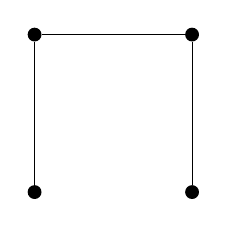
\begin{tikzpicture}[baseline={([yshift=-.5ex]current bounding box.center)}]
                \node[fill, circle, inner sep = 0, minimum size = 5pt] at (0, 0) (1) {};
                \node[fill, circle, inner sep = 0, minimum size = 5pt] at (2, 0) (2) {};
                \node[fill, circle, inner sep = 0, minimum size = 5pt] at (0, -2) (3) {};
                \node[fill, circle, inner sep = 0, minimum size = 5pt] at (2, -2) (4) {};
                \draw (1) -- (2);
                \draw (1) -- (3);
                \draw (2) -- (4);
            \end{tikzpicture}
        \end{gather*}
        Higher powers of a given coordinate would then, for example, give rise to diagrams with loops at a given vertex:
        \begin{gather*}
            A^{-1}_{11}A^{-1}_{12}A^{-1}_{22} =
            \begin{tikzpicture}[baseline={([yshift=-.5ex]current bounding box.center)}]
                \node[fill, circle, inner sep = 0, minimum size = 5pt] at (0, 0) (1) {};
                \node[fill, circle, inner sep = 0, minimum size = 5pt] at (2, 0) (2) {};
                \draw (-0.5, 0) circle (0.5);
                \draw (1) -- (2);
                \draw (2.5, 0) circle (0.5);
            \end{tikzpicture}
        \end{gather*}
    \end{example}

    \begin{remark}[Normalization]
        In practice, one often divides all Gaussian integrals by the quantity $I(A,0)$ to cancel the normalization factor. In the functional setting, this is even imperative since, as mentioned above, the normalization factor diverges for infinite-dimensional spaces.
    \end{remark}

\subsection{Generalizations}

    \newdef{Henstock--Kurzweil integral\footnotemark}{\index{integral!Henstock--Kurzweil}\index{integral!Perron}\index{integral!Denjoy}\index{integral!Luzin}\index{gauge|seealso{integral, Denjoy}}\index{integral!McShane}
    \footnotetext{Also called the \textbf{Perron}, \textbf{Lusin}, \textbf{(narrow) Denjoy} or \textbf{gauge} integral.}
        Consider the usual definition of the (proper) Riemann integral, where tagged partitions $P$ of $[a,b]$ are chosen and the integral is obtained as the limit of the Riemann sums
        \begin{gather}
            I = \sum_Pf(x_i)(t_i-t_{i-1})
        \end{gather}
        as the mesh size of the partitions goes to zero.

        Now, to obtain the generalized integral, consider a strictly positive function $\delta:[a,b]\mathbb{R}^{>0}$, the \textbf{gauge function}. Given such a gauge, a tagged partition $P$ is said to be \textbf{$\delta$-fine} if
        \begin{gather}
            [t_{i-1},t_i]\subset[x_i-\delta(x_i),x_i+\delta(x_i)]
        \end{gather}
        for subintervals in the partition.\footnote{If the condition $x_i\in[t_{i-1},t_i]$ in the definition of tagged partitions is dropped, the \textbf{McShane integral} is obtained. This can be shown to be equivalent to the \textit{Lebesgue integral} (see \labelref{chapter:measure}).}

        If the integral exists, it is given by the number $I\in\mathbb{R}$ such that for all $\varepsilon>0$ there exists a gauge $\delta:[a,b]\rightarrow\mathbb{R}^{>0}$ such that, if $P$ is $\delta$-fine, then
        \begin{gather}
            \left\vert I-\sum_Pf(x_i)(t_i-t_{i-1})\right\vert<\varepsilon\,.
        \end{gather}
    }
    \begin{remark}[Riemann integral]\index{integral!Riemann}
        If the gauge functions are chosen to be constant, the classical $(\varepsilon,\delta)$-definition of ordinary Riemann integrals is obtained.
    \end{remark}

    The following statement can be seen as a refinement of \cref{topology:heine_borel}. Moreover, it is also sometimes known as the \textbf{Borel--Lebesgue theorem}.\index{Borel--Lebesgue}
    \begin{property}[Cousin]\index{Cousin}
        For every gauge $\delta:[a,b]\rightarrow\mathbb{R}^{>0}$, there exists a $\delta$-fine partition. 
    \end{property}

    \begin{property}[Integrability]
        If $f:[a,b]\rightarrow\mathbb{R}$ is bounded, then the following are equivalent:
        \begin{itemize}
            \item $f$ is Henstock--Kurzweil integrable, and
            \item $f$ is \textit{Lebesgue integrable} (see \labelref{chapter:measure}).
        \end{itemize}
        More generally, a function $f:[a,b]\rightarrow\mathbb{R}$ is Henstock--Kurzweil integrable if and only if both $f$ and $|f|$ are \textit{Lebesgue integrable}.
    \end{property}

    The following property shows that `improper' Henstock--Kurzweil integrals are only truly improper for unbounded domains.
    \begin{property}[Hake]\index{Hake}
        \begin{gather}
            \Int_a^bf\,dx = \lim_{c\nearrow b}\Int_a^cf\,dx\,,
        \end{gather}
        whenever either side exists.
    \end{property}

    One of the most important arguments for using the Henstock--Kurzweil integral is its refinement of the Second Fundamental Theorem of Calculus~\ref{calculus:second_fundamental_theorem}. Note that the theorem for the Riemann integral required that the derivative was integrable. The gauge integral relaxes this condition.
    \begin{theorem}[Second fundamental theorem of calculus]
        Let $f:[a,b]\rightarrow\mathbb{R}$ be differentiable, then
        \begin{gather}
            \Int_a^xf'(x')\,dx' = f(x)-f(a)\text{\ \ a.e.}
        \end{gather}
    \end{theorem}

\section{Convexity}

    \newdef{Convex set}{\index{convex}\index{hull}\label{calculus:convex}
        A subset of $X$ of a vector space $V$ (\cref{linalgebra:vector_space}) is said to be convex if $x,y\in X$ implies that $\bigl\{\lambda x+(1-\lambda)y\mid\lambda\in[0,1]\bigr\}\subset X$, i.e.~if all straight lines connecting elements of the set are completely contained in that set. The \textbf{convex hull} of a subset $X$ is defined as the smallest convex subset containing $X$.
    }

    \newdef{Extreme point}{\index{extreme!point}\label{calculus:extreme_point}
        Consider a convex set $X$. The extreme points of $X$ are the points $p\in X$ such that, if
        \begin{gather}
            p = \lambda p_1 + (1-\lambda)p_2
        \end{gather}
        for some $p_1,p_2\in X$ and $\lambda\in[0,1]$, then $p_1=p_2=p$.
    }

    \newdef{Convex function}{\label{calculus:convex_function}
        Let $X$ be a convex set. A function $f:X\rightarrow\mathbb{R}$ is said to be convex if for all $x,y\in X$ and $\lambda\in[0,1]$:
        \begin{gather}
            f\bigl(\lambda x + (1-\lambda)y\bigr)\leq t\lambda(x) + (1-\lambda)f(y)\,.
        \end{gather}
        For the definition of a \textbf{concave} function, the inequality has to be turned around.
    }
    \newdef{Linear map}{\index{linear!map}
        A function $f:X\rightarrow\mathbb{R}$ is linear if and only if it is both convex and concave.
    }

    \begin{theorem}[Karamata's inequality]\index{Karamata}
        Consider an interval $I\subset\mathbb{R}$ and let $f:I\rightarrow\mathbb{R}$ be a convex function. If $(x_1,\ldots,x_n)$ is a tuple that majorizes $(y_1,\ldots,y_n)$, i.e.
        \begin{gather}
            \sum_{i=1}^nx_i = \sum_{i=1}^ny_i
        \end{gather}
        and
        \begin{gather}
            x_{(1)} + \cdots + x_{(k)}\geq y_{(1)} + \cdots + y_{(k)}
        \end{gather}
        for all $k\leq n$, where $x_{(i)}$ denotes the $i^{\text{th}}$ largest element of $(x_1,\ldots,x_n)$, then
        \begin{gather}
            \sum_{i=1}^nf(x_i)\geq\sum_{i=1}^nf(y_i)\,.
        \end{gather}
    \end{theorem}

    The following inequality can be derived directly from the definition of convexity by induction.
    \begin{theorem}[Jensen's inequality]\index{Jensen's inequality}\label{calculus:jensen_inequality}
        Let $f$ be a convex function and consider a point $\{a_i\}_{i\leq n}$ in the probability simplex $\Delta^n$ (\cref{topology:standard_simplex}).
        \begin{gather}
            f\left(\sum_{i=1}^na_ix_i\right)\leq\sum_{i=1}^na_if(x_i)\,.
        \end{gather}
    \end{theorem}

    \newdef{Legendre transformation}{\index{Legendre!transformation}\label{calculus:legendre}
        Consider a function $f:\mathbb{R}\rightarrow\mathbb{R}$. In certain cases (especially in physics) it is sometimes useful to replace the argument $x$ by the slope of $f$ at $x$, i.e.~to perform the transformation
        \begin{gather}
            x\longrightarrow f'(x)\,.
        \end{gather}
        However, it should be clear that this transformation is not always well-defined and, even if it is, it does not always preserve all the information contained in $f$.

        These conditions are satisfied exactly if $f$ is convex (or concave). In this case, the Legendre transform of $f$ is defined as
        \begin{gather}
            f^*(x^*) := \sup_x\bigl(x^*x - f(x)\bigr)\,.
        \end{gather}
        Now, consider the case where $f$ is differentiable. The above supremum can then be obtained by differentiating the right-hand side and equating it to zero. This results in $x^* = f'(x)$, which is exactly the transformation that was required. By expressing everything in terms of the Legendre tranformed quantity $x^*$, one can also find the derivative of $f^*$:
        \begin{gather}
            \deriv{f^*}{x^*}(x^*) = x(x^*)\,.
        \end{gather}
    }

    \begin{property}[Alternative characterization]\label{calculus:legendre_condition}
        In fact, up to an additive constant, the condition
        \begin{gather}
            (f^*)' = (f')^{-1}
        \end{gather}
        uniquely determines the Legendre transformation.
    \end{property}
    \begin{remark}
        These definitions can easily be extended to higher dimensions ($n\geq2$).
    \end{remark}

\section{Umbral calculus}\label{section:umbral_calculus}

    \newdef{Bernoulli polynomial}{\index{Bernoulli!polynomial}\label{calculus:bernoulli_number}
        The Bernoulli polynomials $B_n(x)$, for $n\in\mathbb{N}$, are generated as follows:
        \begin{gather}
            \frac{te^{xt}}{e^t-1} = \sum_{n=0}^{+\infty}B_n(x)\frac{t^n}{n!}\,.
        \end{gather}
        The Bernoulli numbers are defined as
        \begin{gather}
            B_n := B_n(0)\,.
        \end{gather}
    }

    \begin{property}[Recursion]\label{calculus:bernoulli_recursion}
        \begin{gather}
            B_n(x) = \sum_{k=0}^{+\infty}{n \choose k}B_kx^{n-k}
        \end{gather}
        or, more generally,
        \begin{gather}
            B_n(x+y) = \sum_{k=0}^{+\infty}{n \choose k}B_k(x)y^{n-k}
        \end{gather}
    \end{property}

    \begin{formula}[Differential formula]
        \begin{gather}
            B_n(x) = \frac{D}{e^D-1}x^n\,,
        \end{gather}
        where $D\equiv\ds\deriv{}{x}$.
    \end{formula}

    The recursion formula shows that Bernoulli polynomials are a concrete example of a more general class of polynomial sequences.
    \newdef{Appell sequence}{\index{Appell sequence}
        A sequence of polynomials $\seq{p}\subset\mathbb{R}[x]$ that satisfies
        \begin{gather}
            p_n(x+y) = \sum_{k=0}^n{n\choose k}p_k(x)y^{n-k}\,.
        \end{gather}
        This is equivalent to the following recursion relation
        \begin{gather}
            \deriv{p_n}{x} = np_{n-1}\,.
        \end{gather}
    }

    The second recursion relation for Appell sequences can be generalized to arbitrary linear operators. For so-called \textit{delta operators}\index{operator!delta}, i.e.~generalized derivative operators such as the \textit{forward differencing operator}, another important class of polynomials is recovered.
    \newdef{Sheffer sequence}{\index{Sheffer sequence}
        Let $Q:\mathbb{R}[x]\rightarrow\mathbb{R}[x]$ be a \textbf{delta operator}, i.e.~a shift-equivariant operator on polynomial functions that lowers the degree by 1:
        \begin{gather}
            Q\bigl(p(x+\lambda)\bigr) = Qp(x+\lambda)
        \end{gather}
        and
        \begin{gather}
            \deg(Qp) = \deg(p)-1
        \end{gather}
        for all $\lambda\in\mathbb{R}$ and $p\in\mathbb{R}[x]$.

        A polynomial sequence $\seq{p}\subset\mathbb{R}[x]$ is said to be a Sheffer sequence if
        \begin{gather}
            Qp_n = np_{n-1}\,.
        \end{gather}
    }
    \begin{example}
        Many common polynomials form Sheffer sequences, a few examples are Abel, Bernoulli, Euler, Hermite and Laguerre polynomials.
    \end{example}

    \begin{property}[Umbral composition]\index{umbral!composition}\label{calculus:umbral_composition}
        The Sheffer sequences form a group under the following composition law:
        \begin{gather}
            (p\circ q)_n(x) := \sum_{k=0}^na_{n,k}q_k(x) = \sum_{0\leq k\leq l\leq n}a_{n,k}b_{k,l}x^l
        \end{gather}
        where $p_n=\sum_{k=0}^nb_{n,k}x^k$ and $q_n=\sum_{k=0}^na_{n,k}x^k$. The identity element of the umbral group is given by the standard monomials $p_n(x)=x^n$.
    \end{property}

    \newdef{Binomial type}{\index{binomial!type}
        A polynomial sequence $\seq{p}\subset\mathbb{R}[x]$ is said to be of binomial type if
        \begin{gather}
            p_n(x+y) = \sum_{k=0}^n{n\choose k}p_k(x)p_{n-k}(y)\,.
        \end{gather}
        A Sheffer sequence is of binomial type if and only if
        \begin{itemize}
            \item $p_0(x)=1$, and
            \item $p_n(0)=0$ for all $n\in\mathbb{N}_0$.
        \end{itemize}
    }

    \begin{property}[Semidirect product]
        The umbral group is a semidirect product (\cref{group:inner_semidirect_product}) of the (Abelian) subgroup of Appell sequences and the subgroup of binomial type.

        This gives rise to a general recursion relation. Let $\seq{s}$ be a Sheffer sequence and consider the unique sequence $\seq{p}$ of binomial-type polynomials in the same coset as $s$.
        \begin{gather}
            s_n(x+y) = \sum_{k=0}^np_k(x)s_{n-k}(y)
        \end{gather}
    \end{property}

    Now, what about the term `umbral calculus'? In the $19^{\text{th}}$ century, some mathematicians noticed the apparent similarity between the binomial theorem~\ref{calculus:binomial_theorem} for monomials and the recursion relation~\ref{calculus:bernoulli_recursion} for Bernoulli polynomials. (This is, of course, explained by the fact that they are both Appell sequences.) This relation was, in turn, used to `prove' various statements about these polynomials. Passage from one sequence to another happens through a linear operator on the space of Appell sequences, as shown by \indexauthor{Rota}:
    \begin{gather}
        L_B:\mathbb{R}[x]\rightarrow\mathbb{R}[x]:x^n\mapsto B_n\,.
    \end{gather}
    The umbral composition rule is then simply given by the composition~\ref{calculus:umbral_composition} of two such linear operators.

% \chapter{Complex Analysis}

\section{Complex algebra}

    The set of complex numbers $\mathbb{C}$ forms a 2-dimensional vector space over the field of real numbers \ref{chapter:linear_algebra}. At the same time, the operations of complex addition and complex multiplication also turn the complex numbers into a field.

    \newdef{Complex conjugate}{\index{complex conjugate}
        Complex conjugation
        \begin{gather}
            \overline{\,\cdot\,}:a+bi\mapsto a-bi
        \end{gather}
        is an involution \ref{set:involution}. It is sometimes denoted by $z^*$ instead of $\overline{z}$, but unless this would cause confusion the former notation will be used.
    }

    \newformula{Real/imaginary part}{
        \nomenclature[O_Re]{$\mathrm{Re}$}{real part of a complex number}
        \nomenclature[O_Im]{$\mathrm{Im}$}{imaginary part of a complex number}
        A complex number $z$ can also be written as $\mathrm{Re}(z) + i\ \mathrm{Im}(z)$, where
        \begin{align}
            \mathrm{Re}(z) &:= \frac{z + \overline{z}}{2}\\
            \mathrm{Im}(z) &:= \frac{z - \overline{z}}{2i}.
        \end{align}
    }
    \newdef{Argument}{\index{argument}\index{polar!form}
        \nomenclature[O_arg]{$\arg$}{argument of a complex number}
        Let $z$ be a complex number expressed in \textit{polar form}: $z = re^{i\theta}$. The number $\theta$ is called the argument of $z$ and it is denoted by $\arg(z)$.
    }

    \newdef{Riemann sphere}{\index{Riemann!sphere}
        Consider the one-point compactification $\overline{\mathbb{C}} = \mathbb{C}\cup\{\infty\}$ (Definition \ref{topology:alexandrov_compactification}). This set is called the Riemann sphere or \textbf{extended complex plane}. The standard operations on $\mathbb{C}$ can be generalized to $\overline{\mathbb{C}}$ for all nonzero $z\in\mathbb{C}$ in the following way:
        \begin{align}
            z + \infty &:= \infty\nonumber\\
            z * \infty &:= \infty\\
            \frac{z}{\infty} &:= 0.\nonumber
        \end{align}
        Since there exists no multiplicative inverse for $\infty$, the Riemann sphere is not a field.
    }

\section{Holomorphic functions}

    \newdef{Holomorphic function}{\index{holomorphic}
        A function $f$ is said to be holomorphic on an open set $U\subseteq\mathbb{C}$ if it is complex differentiable at every point $z_0\in U$, i.e. for every point $z_0\in U$ the following limit exists:
        \begin{gather}
            f'(z_0) := \lim_{z\rightarrow z_0}\frac{f(z) - f(z_0)}{z-z_0}.
        \end{gather}
    }
    \newdef{Biholomorphic function}{
        A holomorphic function $f$ for which $f^{-1}$ is also holomorphic.
    }
    \newdef{Entire}{\index{entire}
        A function that is holomorphic at every point $z\in\mathbb{C}$.
    }

    \begin{property}[Cauchy-Riemann conditions]\index{Cauchy-Riemann conditions}\label{complex:cauchy_riemann}\index{Wirtinger derivative}
        \nomenclature[A_CR]{CR}{Cauchy-Riemann}
        A holomorphic function $f$ satisfies the following conditions:
        \begin{gather}
            \pderiv{u}{x} = \pderiv{v}{y} \text{\qquad and\qquad} \pderiv{u}{y} = -\pderiv{v}{x}.
        \end{gather}
        These conditions can be combined into one equation using the so-called \textbf{Wirtinger derivative}:
        \begin{gather}
            \label{complex:holomorphic_alternative_condition}
            \pderiv{f}{\overline{z}} = 0.
        \end{gather}
    \end{property}

    \begin{theorem}[Looman-Menchoff\footnotemark]\index{Looman-Menchoff}
        \footnotetext{This is the most general theorem on the holomorphy of continuous functions. It generalizes the original results by \textit{Riemann} and \textit{Cauchy-Goursat}.}
        Let $f$ be a continuous function defined on a subset $U\in\mathbb{C}$. If the partial derivatives of the real and imaginary part exist and if $f$ satisfies the Cauchy-Riemann conditions, then $f$ is holomorphic on $U$.
    \end{theorem}

    \begin{property}[Laplace equation]
        The functions $u,v$ satisfying the CR conditions are harmonic functions, i.e. they satisfy the Laplace equation.
    \end{property}
    \begin{property}[Level sets]
        The functions $u,v$ satisfying the CR conditions have orthogonal level curves \ref{set:level_set}.
    \end{property}

    \begin{property}[Real functions]
        Consider a real-valued function $f$ defined on the complex plane. If it is holomorphic, the CR conditions imply that $f$ is a constant.
    \end{property}

    \begin{theorem}[Identity theorem]\index{identity!theorem}
        If two holomorphic functions on a domain $D$ coincide on a set containing an accumulation point of $D$, they coincide on all of $D$.
    \end{theorem}

\section{Contour integrals}

    \sremark{Whenever contours are considered for integration purposes, they have been chosen to be evaluated counter-clockwise (by convention). To obtain results concerning clockwise evaluation, most of the time adding a minus sign is sufficient.}

    \newdef{Contour integral}{\index{integral!contour}\label{complex:contour_integral}
        The contour integral of a function $f(z)=u(z)+iv(z)$ is defined as the following line integral:
        \begin{gather}
            \int_{z_1}^{z_2}f(z)dz = \int_{(x_1,y_1)}^{(x_2,y_2)}\big[u(x,y) + iv(x,y)\big](dx+idy).
        \end{gather}
    }

    \begin{theorem}[Cauchy's integral theorem\footnotemark]\index{Cauchy!integral theorem}\index{rectifiable curve}\label{complex:cauchy_integral_theorem}
        \footnotetext{Also called the \textbf{Cauchy-Goursat theorem}.}
        Let $\Omega$ be a simply-connected subset of $\mathbb{C}$ and let $f$ be a holomorphic function on $\Omega$. For every closed, rectifiable (i.e. of finite length) contour $C$ in $\Omega$:
        \begin{gather}
            \oint_Cf(z)dz = 0.
        \end{gather}
    \end{theorem}
    \begin{result}[Freedom of contour]
        The contour integral of a holomorphic function depends only on the limits of integration and not on the contour connecting them.
    \end{result}

    \begin{formula}[Cauchy's integral formula]\index{Cauchy!integral formula}\label{complex:cauchy_integral_formula}
        Let $\Omega$ be a connected subset of $\mathbb{C}$ and let $f$ be a holomorphic function on $\Omega$. Consider a contour $C$ in $\Omega$. For every point $z_0$ inside $C$ one can express the function $f$ as follows:
        \begin{gather}
            f(z_0) = \frac{1}{2\pi i}\oint_C\frac{f(z)}{z-z_0} dz.
        \end{gather}
    \end{formula}

    \begin{result}[Analytic function]\index{analytic!function}
        Let $\Omega$ be a connected subset of $\mathbb{C}$ and let $C$ be a closed contour in $\Omega$. If $f$ is holomorphic on $\Omega$, then $f$ is analytic \ref{calculus:analytic} on $\Omega$ and
        \begin{gather}
            \label{complex:cauchy_integral_formula_derivative}
            f^{(n)}(z_0) = \frac{1}{2\pi i}\oint_Cf(z)\frac{n!}{(z-z_0)^{n+1}} dz.
        \end{gather}
        Furthermore, the derivatives are also holomorphic on $\Omega$.
    \end{result}

    \begin{theorem}[Morera]\index{Morera}
        If $f$ is continuous on a connected open set $\Omega$ and $\oint_Cf(z)dz = 0$ for every closed contour $C$ in $\Omega$, then $f$ is holomorphic on $\Omega$.
    \end{theorem}

    \begin{theorem}[Liouville]\index{Liouville!theorem on entire functions}
        Every bounded entire function is constant.
    \end{theorem}

    \begin{theorem}[Sokhotski-Plemelj]\index{Sokhotski-Plemelj}\label{complex:sokhotski_plemelj}
        Let $f$ be a continuous complex-valued function defined on the real line and let $a<0<b$, then
        \begin{gather}
            \lim_{\varepsilon\rightarrow0^+}\int_a^b\frac{f(x)}{x\pm i\varepsilon}dx = \mp i\pi f(0) + \mathcal{P}\int_a^b\frac{f(x)}{x}dx,
        \end{gather}
        where $\mathcal{P}$ denotes the Cauchy principal value.
    \end{theorem}

\section{Laurent series}

    \begin{definition}[Laurent series]\index{Laurent!series}\index{annulus}\index{principal!part}\label{complex:laurent_series}
        If $f$ is a analytic function defined on an \textbf{annulus}, i.e. a ring-shaped region, then $f$ can be expanded as the following series:
        \begin{gather}
            f(z) = \sum^\infty_{n=-\infty}a_n(z - z_0)^n \qquad\text{with}\qquad a_n = \frac{1}{2\pi i}\oint\frac{f(z')}{(z'-z_0)^{n+1}} dz'.
        \end{gather}
        The subseries containing all negative degree terms is called the \textbf{principal part} of the Laurent series.
    \end{definition}

    \begin{property}[Convergence of Lauren series]
        The Laurent series of an analytic function $f$ converges uniformly to $f$ on the annulus $R_1 < |z-z_0| < R_2$, with $R_1$ and $R_2$ the distances from $z_0$ to the two closest \textit{poles}.
    \end{property}

    \newdef{Analytic continuation}{\index{analytic!continuation}
        Consider an analytic function $f$ defined on an open subset $U\subset\mathbb{C}$. If $V\subset\mathbb{C}$ is an open subset containing $U$ and if there exists an analytic function $F$ on $V$ such that $F(z)=f(z)$ for all $z\in U$, then $F$ is called the analytic continuation of $f$ to $V$. Using the identity theorem for holomorphic functions one can prove that analytic continuations are unique (on connected domains).
    }

    \begin{theorem}[Schwarz's reflection principle]\index{Schwarz!reflection principle}
        Let $f$ be analytic on the upper half plane. If $z\in\mathbb{R}\implies f(z)\in\mathbb{R}$, then
        \begin{gather}
            f(\overline{z}) = \overline{f(z)}.
        \end{gather}
    \end{theorem}

\section{Singularities}
\subsection{Poles}

    \newdef{Pole}{\index{pole}\label{complex:pole}
        A function $f$ has a pole of order $m>0$ at a point $z_0$ if its Laurent series at $z_0$ satisfies $\forall n<-m:a_n = 0$ and $a_{-m}\neq0$.
    }

    \newdef{Meromorphic}{\index{meromorphic}
        A function $f$ is said to be meromorphic if it is analytic on the whole complex plane with exception of isolated poles and removable singularities. Every meromorphic function can be written as a fraction of two holomorphic functions, where the poles coincide with the zeros of the denominator.
    }

    \newdef{Essential singularity}{\index{essential!singularity}
        A function $f$ has an essential singularity at a point $z_0$ if its Laurent series at $z_0$ satisfies $\forall n\in\mathbb{N}:a_{-n}\neq0$, i.e. if its Laurent series has infinitely many negative degree terms.
    }

    \newmethod{Frobenius transformation}{\index{Frobenius!transformation}
        To study the behaviour of a function $f$ at $z\rightarrow\infty$, one can apply the Frobenius transformation $h = 1/z$ and study the limit $\lim_{h\rightarrow0}f(h)$. For example, a singularity at $\infty$ is defined as a singularity of $f(1/z)$ at 0.
    }
    \begin{property}[Polynomials]\index{poly-!nomial}
        An entire function $f$ is polynomial if and only if it has a pole at $\infty$.
    \end{property}

    \begin{theorem}[Casorati-Weierstrass]\index{Casorati-Weierstrass}
        Let $f$ be holomorphic on the punctured open set $U\backslash\{z_0\}$ with an essential singularity at $z_0$. For every neighbourhood $V$ of $z_0$ contained in $U$, the image $f(V\backslash\{z_0\})$ is dense in $\mathbb{C}$.
    \end{theorem}
    \begin{result}
        If $f$ is an entire nonpolynomial function, then for every $c\in\mathbb{C}$ there exists a sequence $z_n\longrightarrow\infty$ such that $f(z_n)\longrightarrow c$.\footnote{Polynomials are excluded due to the property above.}
    \end{result}

    \begin{theorem}[Picard's little theorem]\index{Picard}
        The range of a nonconstant entire function is the complex plane with at most a single exception.
    \end{theorem}
    \begin{theorem}[Picard's great theorem]
        Let $f$ be an analytic function with an essential singularity at $z_0$. On every punctured neighbourhood of $z_0$, $f$ takes on all possible values, with at most a single exception, infinitely many times.
    \end{theorem}

\subsection{Branch cuts}

    \newformula{Roots}{\index{root}
        Let $z\in\mathbb{C}$. The $n^{th}$ roots\footnote{Also see the fundamental theorem of algebra \ref{alggeom:fundamental_theorem_of_algebra}.} of $z = re^{i\theta}$ are given by
        \begin{gather}
            \left\{\sqrt[n]{r}\exp\left(i\frac{\theta + 2\pi k}{n}\right)\,\middle\vert\,k\in\{0,1,\ldots,n\}\right\}.
        \end{gather}
    }
    \newformula{Complex logarithm}{\index{logarithm}
        The natural logarithm can be continued to the complex plane (as a multi-valued function) as follows:
        \begin{gather}
            \mathrm{LN}(z) := \{\ln(r) + i(\theta + 2\pi k)\mid k\in\mathbb{Z}\}.
        \end{gather}
    }

    \newdef{Branch}{\index{branch}
        The problem with the previous two formulas is that they represent multi-valued functions. To get an unambiguous image it is necessary to fix a value of the parameter $k$. By doing so there will arise curves, called \textbf{branch cuts}, in the complex plane where the function becomes discontinuous. A \textbf{branch} is defined as a particular choice of the parameter $k$.

        For the logarithm the choice for $\arg(\mathrm{LN})\in\ ]\alpha, \alpha + 2\pi]$ is often denoted by $\mathrm{LN}_\alpha$ or $\log_\alpha$.
    }
    \newdef{Principal value}{\index{principal!value}
        The principal value of a multi-valued complex function is defined as the value associated with a choice of branch for which $\arg(f)\in\ ]-\pi,\pi]$.
    }

    \newdef{Branch point}{
        Let $f$ be a complex-valued function. A point $z_0$ for which there exists no neighbourhood on which $f$ is single-valued is called a branch point.
    }
    \newdef{Branch cut}{
        A line connecting exactly two branch points, one possibly being $\infty$, is called a branch cut. In case there exist multiple branch cuts, they are required to never cross.
    }

    \begin{example}
        Consider the complex function \[f(z) = \frac{1}{\sqrt{(z-z_1)\cdots(z-z_n)}}.\] This function has singularities at $z_1,\ldots,z_n$. If $n$ is even, this function will have $n$ (finite) branch points. This implies that the points can be grouped in pairs connected by non-intersecting branch cuts. If $n$ is odd, this function will have $n$ (finite) branch points and one branch point at infinity. The finite branch points will be grouped in pairs connected by non-intersecting branch cuts and the remaining branch point will be joined to infinity by a branch cut that does not intersect the others.
    \end{example}

\subsection{Residue theorem}\index{residue}

    \newdef{Residue}{\label{complex:residue_def}
        \nomenclature[O_Res]{$\mathrm{Res}$}{residue of a complex function}
        By applying Formula \ref{complex:contour_integral} to a polynomial function, one finds
        \begin{gather}
            \int_C(z-z_0)^ndz = 2\pi i\delta_{n,-1},
        \end{gather}
        where $C$ is a contour around the pole $z=z_0$. This means that integrating a Laurent series around a pole isolates the coefficient $a_{-1}$. This coefficient is, therefore, called the residue of the function at the given pole.
    }
    \begin{notation}
        The residue of a complex function $f$ at a pole $z_0$ is denoted by \[\mathrm{Res}[f(z)]_{z=z_0}.\]
    \end{notation}

    \begin{formula}
        For a pole of order $m$, the residue is calculated as follows:
        \begin{gather}
            \label{complex:residue}
            \mathrm{Res}\left[f(z)\right]_{z=z_j} = \lim_{z\rightarrow z_0}\frac{1}{(m - 1)!} \left(\pderiv{}{z}\right)^{m-1}\left(f(z)(z-z_0)\right).
        \end{gather}
        For essential singularities the residue can be found by writing out the Laurent series explicitly.
    \end{formula}

    \begin{theorem}[Residue theorem]\label{complex:residue_theorem}
        If $f$ is a meromorphic function on $\Omega$ and if $C$ is a closed contour in $\Omega$ that contains the poles $z_j$ of $f$, then
        \begin{gather}
            \oint_Cf(z)dz = 2\pi i\sum_j\mathrm{Res}\left[f(z)\right]_{z=z_j}.
        \end{gather}
        For poles on the contour $C$, only half of the residue contributes to the integral.
    \end{theorem}

    \begin{formula}[Argument principle]\index{argument!principle}
        Let $f$ be a meromorphic function and denote the number of zeros and poles of $f$ inside the contour $C$ by $Z_f(C)$ and $P_f(C)$, respectively. From the residue theorem one can derive the following formula:
        \begin{gather}
            \frac{1}{2\pi i}\oint_C\frac{f(z)}{f'(z)}dz = Z_f(C) - P_f(C).
        \end{gather}
    \end{formula}
    \begin{definition}[Winding number]\index{winding number}\index{index!of map}
        \nomenclature[O_Ind]{$\mathrm{Ind}_f(z)$}{index of a point $z\in\mathbb{C}$ with respect to a function $f$}
        Let $f$ be a meromorphic function and let $C$ be a simple closed contour. For all $a\not\in f(C)$ the winding number, also called the \textbf{index}, of $a$ with respect to the function $f$ is defined as follows:
        \begin{gather}
            \mathrm{Ind}_f(a) := \frac{1}{2\pi i}\oint_C\frac{f'(z)}{f(z) - a}dz.
        \end{gather}
        This number is always an integer.
    \end{definition}

\section{Limit theorems}

    \begin{theorem}[Small limit theorem]\index{limit!theorem}\label{complex:small_limit}
        Let $f$ be a function that is holomorphic almost everywhere on $\mathbb{C}$ and let the contour $C$ be a circular segment with radius $\varepsilon$ and central angle $\alpha$. If $z$ is parametrized as $z = \varepsilon e^{i\theta}$, then\[\int_Cf(z)dz = i\alpha A\] with \[A = \lim_{\varepsilon\rightarrow0}f(z).\]
    \end{theorem}

    \begin{theorem}[Great limit theorem]\label{complex:great_limit}
        Let $f$ be a function that is holomorphic almost everywhere on $\mathbb{C}$ and let the contour $C$ be a circular segment with radius $R$ and central angle $\alpha$. If $z$ is parametrized as $z = Re^{i\theta}$, then \[\int_Cf(z)dz = i\alpha B\] with \[B = \lim_{R\rightarrow\infty}f(z).\]
    \end{theorem}

    \begin{theorem}[Jordan's lemma]\index{Jordan}\label{complex:jordan}
        Let $g$ be a continuous function that can be written as $g(z) = f(z)e^{bz}$ and let the contour $C$ be a semicircle lying in the half-plane bounded by the real axis and oriented away of the point $i\overline{b}$. If $z$ is parametrized as $z=Re^{i\theta}$ and \[\lim_{R\rightarrow\infty}f(z) = 0,\] then \[\int_Cg(z)dz = 0.\]
    \end{theorem}
\chapter{Measure \& Integration Theory}\label{chapter:measure}

    The main references for this chapter are~\citet{capinski_measure_2013,choquet-bruhat_analysis_1991}.

    \minitoc

\section{Measure theory}
\subsection{General definitions}

    \newdef{Measure}{\index{measure}\index{outer!measure}\index{$\sigma$!additivity}\label{measure:measure}
        Let $X$ be a set and let $\Sigma$ be a $\sigma$-algebra over $X$. A function $\mu:\Sigma\rightarrow\overline{\mathbb{R}}$ is called a measure if it satisfies the following conditions:
        \begin{enumerate}
            \item\textbf{Nonnegativity}: $\forall E\in\Sigma:\mu(E)\geq0$,
            \item\textbf{Empty set is null}: $\mu(\emptyset)=0$, and
            \item\textbf{$\sigma$-additivity}: $\forall i\neq j:E_i\cap E_j=\emptyset\implies\mu\left(\bigcup_{n=1}^\infty E_n\right) = \sum_{i=n}^{+\infty}\mu(E_n)$.
        \end{enumerate}
        When $\mu$ is defined on all of $P(X)$ and only satisfies countable subadditivity, i.e.~the equality in the last condition becomes an inequality $\leq$, it is called an \textbf{outer measure}.
    }
    \begin{remark}
        To show that two measures coincide on a $\sigma$-algebra, it suffices to show that they coincide on the generating sets and apply the Monotone Class Theorem~\ref{set:monotone_class}.
    \end{remark}

    \newdef{Measure space}{\label{measure:measure_space}\index{measurable!set}
        The pair $(X,\Sigma)$ is called a measurable space and the triple $(X,\Sigma,\mu)$ is called a measure space. The elements $E\in\Sigma$ are called \textbf{measurable sets}.
    }

    \newdef{Null set}{\index{null!set}
        A set $A\subset\mathbb{R}$ is said to be null if $\mu(A)=0$.
    }

    \newdef{Almost everywhere\footnotemark}{\index{almost everywhere}\label{measure:almost_everywhere}
        \footnotetext{In probability theory this is often called \textbf{almost surely}.}
        Let $(X,\Sigma,\mu)$ be a measure space. A property $P$ is said to hold on $X$ almost everywhere (abbreviated as \textbf{a.e.}) if it satisfies the following equation:
        \begin{gather}
            \mu\bigl(\{x\in X\bigm\vert\neg P(x)\}\bigr) = 0\,,
        \end{gather}
        i.e.~it holds everywhere except for a null set.
    }

    \newdef{Complete measure space}{\index{complete!measure space}
        A measure space $(X,\Sigma,\mu)$ is said to be complete if for every $E\in\Sigma$ with $\mu(E)=0$ the implication $A\subset E\implies A\in\Sigma$ holds. Additivity then necessarily implies that $\mu(A)=0$.
    }
    \newdef{Completion}{
        Let $\Sigma\subseteq\overline{\Sigma}$ be $\sigma$-algebras on a set $X$. $(X,\overline{\Sigma},\overline{\mu})$ is called the completion of $(X,\Sigma,\mu)$ if:
        \begin{enumerate}
            \item $\forall A\in\Sigma:\overline{\mu}(A)=\mu(A)$,
            \item $(X,\overline{\Sigma},\overline{\mu})$ is complete, and
            \item $\overline{\Sigma}$ is the smallest $\sigma$-algebra with these properties.
        \end{enumerate}
    }

    \newdef{\texorpdfstring{$\sigma$-}{sigma-}finite measure}{\index{$\sigma$!finite}\label{measure:sigma_finite_measure}
        Let $(X,\Sigma,\mu)$ be a measure space. The measure $\mu$ is said to be $\sigma$-finite if there exists a sequence $\seq{A}$ of measurable sets such that $\bigcup_{n=1}^\infty A_n=X$ with $\forall n\in\mathbb{N}:\mu(A_n)<\infty$.
    }

    \newdef{Borel measure}{\index{Borel!measure}
        Consider a topological space together with its Borel $\sigma$-algebra (\cref{topology:borel_set}). Any measure defined on this measurable space is called a Borel measure.
    }

    \newdef{Locally finite measure}{
        A measure on a Hausdorff space whose measurable sets contain the Borel sets such that every point has an open neighbourhood of finite measure. On locally compact spaces, this is equivalent to requiring that every compact subset has finite measure.
    }

    Given a Borel measure on a topological space, there are different ways of how one can approximate the measure of Borel sets by those of open or closed sets. Sadly, different distinct definitions can be found in the literature all under the name of `regular' measure. The next definition gives the most widely used ones.
    \newdef{Regular measure}{\label{measure:regular_measure}
        An outer measure $\mu$ on a topological space $X$ whose completion contains the Borel sets is said to be \textbf{Borel regular} if for every set $A\subset X$, there exists a Borel set $B\subseteq A$ such that $\mu(A)=\mu(B)$.

        Let $\mu$ be a measure on $(X,\Sigma)$, where $X$ is a topological space. It is said to be \textbf{regular} if if it satisfies the following conditions for every measurable set $B$:
        \begin{enumerate}
            \item\textbf{Outer regularity}: $\mu(B)=\inf\bigl\{\mu(O)\bigm\vert O\text{ open and measurable},O\supset B\bigr\}$, and
            \item\textbf{Inner regularity}: $\mu(B)=\sup\bigl\{\mu(K)\bigm\vert K\text{ closed and measurable},K\subset B\bigr\}$.
        \end{enumerate}
        If $X$ is Hausdorff, the measure is said to be \textbf{regular} if it satisfies the following conditions for every measurable set $B$:
        \begin{enumerate}
            \item\textbf{Outer regularity}: $\mu(B)=\inf\bigl\{\mu(O)\bigm\vert O\text{ open and measurable},O\supset B\bigr\}$, and
            \item\textbf{Inner regularity} or \textbf{tightness}: $\mu(B)=\sup\bigl\{\mu(K)\bigm\vert K\text{ compact and measurable},K\subset B\bigr\}$.
        \end{enumerate}
        Note that since compact subsets of Hausdorff spaces are closed, tight measures are in particular regular.
    }

    By slightly modifying the definition of tight Borel measures, one can obtain yet another type of regularity.
    \newdef{Radon measure}{\index{Radon!measure}\index{locally!finite}\label{measure:radon_measure}
        A Borel measure on a Hausdorff space that is outer regular on Borel sets, inner regular on open sets and locally finite. (For locally compact spaces, outer regularity is superfluous.)
    }

    \newdef{Radon space}{\index{Radon!space}
        A topological space on which every finite Borel measure is Radon. It is sometimes called \textbf{strongly Radon} if every locally finite Borel measure is Radon.
    }
    \begin{example}
        Locally compact, separable metric space, Polish spaces and even Suslin spaces (\cref{metric:suslin}) are Radon. Slightly weaker, every finite Borel measure on a metric space is regular.
    \end{example}

\subsection{Lebesgue measure}

    \newdef{Lebesgue outer measure}{\index{Lebesgue!outer measure}\label{measure:outer_measure}
        Let $X\subseteq\mathbb{R}$ be a set. The (Lebesgue) outer measure of $X$ is defined as follows:
        \begin{gather}
            \lambda^*(X) := \inf\left\{\sum_{n=1}^{+\infty}l(I_n)\,\middle\vert\,\seq{I}\text{ a sequence of open intervals that covers }X\right\}\,.
        \end{gather}
    }

    \begin{property}[Intervals]
        The outer measure of an interval $I$ equals its length: $\lambda^*(I)=l(I)$.
    \end{property}
    \begin{property}[Translation-invariance]\label{measure:translation_invariant}
        The outer measure is translation-invariant:
        \begin{gather}
            \lambda^*(A+t) = \lambda^*(A)
        \end{gather}
        for all $A\subset\mathbb{R}$ and $t\in\mathbb{R}$.
    \end{property}

    \begin{theorem}[Carath\'eodory's criterion]\index{Carath\'eodory!criterion}\index{Lebesgue!measure}\index{measurable!set}\label{measure:lebesgue_measure}
        Let $X$ be a subset of $\mathbb{R}$. If $X$ satisfies the following equation, it is said to be \textbf{Lebesgue measurable}:
        \begin{gather}
            \forall A\subseteq\mathbb{R}:\lambda^*(A) = \lambda^*(A\cap X) + \lambda^*(A\cap X^c)\,.
        \end{gather}
        The collection of all Lebesgue-measurable sets is denoted by $\mathcal{M}$ and the outer measure $\lambda^*(X)$, now denoted by $\lambda$, is called the \textbf{Lebesgue measure} of $X$.
    \end{theorem}
    \begin{result}\label{measure:completion_remark}
        The Lebesgue $\sigma$-algebra $\mathcal{M}$ is the completion of the Borel $\sigma$-algebra $\mathcal{B}$. (This is how the Lebesgue $\sigma$-algebra was introduced historically.)
    \end{result}

    \begin{property}\label{measure:countable_set_is_null}
        Any countable set is null with respect to the Lebesgue outer measure.
    \end{property}

    \begin{property}[Regularity]
        The Lebesgue measure is a regular Borel measure. For every $A\subseteq\mathbb{R}$, there exists a sequence $\seq{O}$ of open sets such that
        \begin{gather}
            \label{measure:open_cover_existence}
            A\subset\bigcap_{n=1}^{+\infty} O_n\qquad\text{and}\qquad\lambda\left(\bigcap_{n=1}^{+\infty} O_n\right) = \lambda^*(A)\,,
        \end{gather}
        and for every $E\in\mathcal{M}$, there exists a sequence $\seq{F}$ of closed sets such that
        \begin{gather}
            \label{measure:closed_cover_existence}
            \bigcup_{n=1}^{+\infty} F_n\subset E\qquad\text{and}\qquad\lambda\left(\bigcup_{n=1}^{+\infty} F_n\right) = \lambda(E)\,.
        \end{gather}
    \end{property}

    \begin{property}
        Consider a set $A\subset\mathbb{R}$. $A\in\mathcal{M}$ if and only if for every $\varepsilon>0$ there exist an open set $O\supset A$ and a closed set $F\subset A$ such that $\lambda^*(O\backslash A) < \varepsilon$ and $\lambda^*(A\backslash F)<\varepsilon$.
    \end{property}

    \begin{property}
        Let $\seq{A}$ be a sequence of sets in $\mathcal{M}$. The following two properties apply:
        \begin{align}
            \forall i\in\mathbb{N}:A_i\subseteq A_{i+1} &\implies \lambda\left(\bigcup_{n=1}^{+\infty} A_n\right) = \lim_{n\rightarrow\infty}\lambda(A_n)\,,\\
            \forall i\in\mathbb{N}:A_i\supseteq A_{i+1}\land\lambda(A_1)<+\infty &\implies\lambda\left(\bigcap_{i=n}^{+\infty} A_n\right) = \lim_{n\rightarrow\infty}\lambda(A_n)\,.
        \end{align}
    \end{property}
    \remark{This property is valid for every $\sigma$-additive set function.}

    \begin{construct}[Restriction]\index{Lebesgue!restricted measure}\label{measure:restricted_lebesgue_measure}
        Let $A\in\mathcal{M}$ have nonzero measure. The restriction of the Lebesgue measure to the set $B$ is defined as follows:
        \begin{gather}
            \mathcal{M}_A := \{A\cap B\mid B\in\mathcal{M}\} \qquad\text{and}\qquad \forall E\in\mathcal{M}_A:\lambda_A(E) := \lambda(E)\,.
        \end{gather}
        It can be shown that the measure space $(A,\mathcal{M}_A,\lambda_A)$ is complete.
    \end{construct}

    The construction of Lebesgue measurable sets from the Lebesgue outer measure can be generalized to arbitrary sets and outer measures.
    \begin{construct}[Carath\'eodory's extension theorem\footnotemark]\index{pre-!measure}\index{Hahn--Kolmogorov}\label{measure:caratheodory}
        \footnotetext{Also called the \textbf{Hahn--Kolmogorov theorem}.}
        Every outer measure $\mu^*$ gives rise to a $\sigma$-algebra consisting of those sets that satisfy Carath\'eodory's criterion (\cref{measure:lebesgue_measure}) with respect to $\mu^*$. Furthermore, consider a \textbf{premeasure} $\mu_0$, i.e.~a $\sigma$-additive function defined on an algebra of sets (\cref{set:algebra_of_sets}) such that $\mu_0(\emptyset) = 0$. \Cref{measure:outer_measure} can be used to define an outer measure $\mu^*$ in terms of the premeasure $\mu_0$ by replacing intervals with elements from the given algebra of sets. The $\sigma$-algebra generated by this outer measure contains the given algebra of sets and $\mu^*$ restricts to $\mu_0$. This shows that any premeasure can be extended to a genuine measure, uniquely if $\mu_0$ is $\sigma$-finite. Moreover, it can be shown that this measure is complete.
    \end{construct}

\subsection{Measurable functions}

    \newdef{Measurable function}{\index{measurable!function}
        Consider two measurable spaces $(X,\Sigma_X)$ and $(Y,\Sigma_Y)$. A function $f:X\rightarrow Y$ is said to be measurable if for every measurable set $A\in\Sigma_Y$ the preimage $f^{-1}(A)$ is also measurable. Equivalently, the $\sigma$-algebra generated by the preimages of measurable sets in $\Sigma_Y$ should be a sub-$\sigma$-algebra of $\Sigma_X$.
    }
    \begin{property}
        Measurability is closed under composition. This turns the collection of measurable spaces and measurable functions into a category $\mathbf{Meas}$. (This notation is also used for the subcategory on \textit{measure spaces} (\cref{measure:measure_preserving}).)
    \end{property}

    \newdef{Measurable}{\index{measurable}
        Sometimes an equivalence class of real- or complex-valued measurable functions up to functions that are zero a.e.~is called a measurable.
    }

    Two important examples are given below:
    \begin{example}[Borel-measurable function]\label{measure:borel_measurable_function}
        A continuous function $f:X\rightarrow Y$ such that for every open set $O\in\mathcal{B}_Y:f^{-1}(O)\in\mathcal{B}_X$.
    \end{example}
    \begin{example}[Lebesgue-measurable function]\label{measure:measurable_function}
        A function $f:\mathbb{R}\rightarrow\mathbb{R}$ such that for every interval $I\subset\mathbb{R}:f^{-1}(I)\in\mathcal{M}$.
    \end{example}
    \remark{The inclusion $\mathcal{B}\subset\mathcal{M}$ implies that every Borel-measurable function is also Lebesgue-measurable.}

    \begin{property}
        The class of Borel/Lebesgue-measurable functions defined on $E\in\mathcal{M}$ forms an algebra.
    \end{property}

    \begin{example}
        The following types of functions are Lebesgue-measurable:
        \begin{itemize}
            \item monotonic functions,
            \item continuous functions, and
            \item indicator functions.
        \end{itemize}
    \end{example}
    \begin{result}
        Let $f,g$ be Lebesgue-measurable functions and let $F:\mathbb{R}\times\mathbb{R}\rightarrow\mathbb{R}$ be a continuous function. The composition $F\bigl(f(x),g(x)\bigr)$ is also measurable.
    \end{result}

    \begin{property}
        Let $f$ be a Lebesgue-measurable function. The level set $\{x\mid f(x)=a\}$ is measurable for all $a\in\mathbb{R}$.
    \end{property}

    \begin{property}
        Define the following functions (which are measurable if $f$ is measurable as a result of the previous properties):
        \begin{align}
            \label{measure:positive_part}
            f^+(x) &:= \max(f,0) =
            \begin{cases}
                f(x)&\cif f(x)>0\\
                0&\cif f(x)\leq0,
            \end{cases}\\\nonumber\\
            \label{measure:negative_part}
            f^-(x) &:= \max(-f,0) =
            \begin{cases}
                0&\cif f(x)>0\\
                -f(x)&\cif f(x)\leq0\,.
            \end{cases}
        \end{align}
        The function $f:\mathbb{R}\rightarrow\mathbb{R}$ is measurable if and only if both $f^+$ and $f^-$ are measurable. Furthermore, $f$ is measurable if $|f|$ is measurable (the converse is false in general).
    \end{property}

    \newdef{Pushforward}{\index{pushforward!of a measure}
        Consider two measurable spaces $(X_1,\Sigma_1)$ and $(X_2,\Sigma_2)$ together with a measurable function $f:X_1\rightarrow X_2$. For every measure $\mu$ on $X_1$ one can define the pushforward measure $f_*\mu$ on $X_2$ as follows:
        \begin{gather}
            f_*\mu(A) := \mu\bigl(f^{-1}(A)\bigr)\,.
        \end{gather}
    }

    \newdef{Measure-preserving function}{\label{measure:measure_preserving}
        Let $(X,\Sigma,\mu)$ be a measure space and consider a measurable function $T:X\rightarrow X$. $T$ is said to be measure-preserving if
        \begin{gather}
            T_\ast\mu = \mu\,.
        \end{gather}
        These functions form the morphisms in the category $\mathbf{Meas}$ of measure spaces.
    }

    \newdef{Ergodic function}{\index{ergodic}
        Let $(X,\Sigma,\mu)$ be a measure space and consider a measure-preserving function $T:X\rightarrow X$. It is said to be ergodic if the following condition is satisfied:
        \begin{gather}
            T(A) = A\implies\mu(A) = 0\lor\mu(X\backslash A) = 0\,.
        \end{gather}
        This is equivalent to stating that for every set $A\in\Sigma$ with positive measure the following condition holds:
        \begin{gather}
            \mu\left(\bigcup_{n=1}^{+\infty} T^{-n}(A)\right) = 1\,.
        \end{gather}
    }

    \begin{property}
        Consider a topological space $X$ with Borel $\sigma$-algebra $\mathcal{B}$ and let $T$ be an ergodic function. Almost every $T$-orbit is dense in the support of $\mu$.
    \end{property}

    \newdef{Mixing}{\index{mixing}
        An endomorphism of a measure spaces $(X,\Sigma,\mu)$ is said to be mixing if for all measurable spaces $A,B$ the following equality holds:
        \begin{gather}
            \lim_{n\rightarrow\infty}\mu\left(T^{-n}(A)\cap B\right) = \mu(A)\mu(B)\,
        \end{gather}
    }
    \begin{property}
        All mixing transformations are ergodic.
    \end{property}

    \begin{property}[Additivity]\index{additive!function}
        Every measurable, additive function $f:\mathbb{R}\rightarrow\mathbb{R}$ is linear.
    \end{property}
    \begin{result}
        From the basic properties of exponential and logarithmic functions, the following results can be obtained:
        \begin{itemize}
            \item Let $f:\mathbb{R}\rightarrow\mathbb{R}$ be a measurable function. If $f(x+y) = f(x)f(y)$, then $f(x)=e^{\lambda x}$ for some $\lambda\in\mathbb{R}$.
            \item Let $f:[0,+\infty]\rightarrow\mathbb{R}$ be a measurable function. If $f(xy) = f(x)+f(y)$, then $f(x)=\lambda\log(x)$ for some $\lambda\in\mathbb{R}$.
            \item Let $f:[0,+\infty]\rightarrow[0,+\infty]$ be a measurable function. If $f(xy) = f(x)f(y)$, then $f(x)=x^\lambda$ for some $\lambda\in\mathbb{R}$.
        \end{itemize}
    \end{result}

\subsection{Limit operations}

    \begin{property}
        Let $\seq{f}$ be a sequence of measurable functions. The following functions are also measurable:
        \begin{itemize}
            \item $\ds\min_{i\leq k}(f_i)$ and $\ds\max_{i\leq k}(f_i)$,
            \item $\ds\inf_{n\in\mathbb{N}}(f_n)$ and $\ds\sup_{n\in\mathbb{N}}(f_n)$, and
            \item $\ds\liminf_{n\rightarrow\infty}(f_n)$ and $\ds\limsup_{n\rightarrow\infty}(f_n)$.
        \end{itemize}
    \end{property}

    \begin{property}
        If $f$ is a measurable function and $g$ is a function such that $f=g$ almost everywhere, then $g$ is measurable as well.
    \end{property}
    \result{As a result of the previous two properties, if a sequence of measurable functions converges pointwise a.e., the limit is also a measurable function.}

    \newdef{Essential supremum}{\index{essential!supremum}\label{measure:essential_supremum}
        \begin{gather}
            \esssup(f) := \inf\{z\in\mathbb{R}\mid f\leq z\text{ a.e.}\}
        \end{gather}
    }
    \newdef{Essential infimum}{\index{essential!infimum}\label{measure:essential_infimum}
        \begin{gather}
            \essinf(f) := \sup\{z\in\mathbb{R}\mid f\geq z\text{ a.e.}\}
        \end{gather}
    }
    \begin{property}
        Every measurable function $f$ satisfies the following inequalities:
        \begin{itemize}
            \item $f\leq\esssup(f)\text{ a.e.}$ and $f\geq\essinf(f)\text{ a.e.}$, and
            \item $\esssup(f)\leq\sup(f)$ and $\essinf(f)\geq\inf(f)$.
        \end{itemize}
        The latter pair of inequalities becomes a pair of equalities if $f$ is continuous.
    \end{property}
    \begin{property}
        If $f,g$ are measurable functions, then $\esssup(f+g)\leq\esssup(f)+\esssup(g)$. An analogous inequality holds for the essential infimum.
    \end{property}

    \newdef{Weak convergence}{\index{convergence!weak}\index{continuity!set}\label{measure:weak_convergence}
        A sequence of measures $\seq{\mu}$ is said to converge weakly to a measure $\mu$ on a metrizable space $X$ if any of the following conditions is satisfied:
        \begin{enumerate}
            \item $\int_Xf\,d\mu_n\longrightarrow\int_Xf\,d\mu$ for all bounded, continuous functions $f$.
            \item $\mu_n(A)\longrightarrow\mu(A)$ for all \textbf{continuity sets} $A$ of $\mu$, i.e.\ for all Borel sets $A$ such that $\mu(\partial A)=0$.
            \item $\lim\inf\mu_n(U)\geq\mu(U)$ for all open sets $U$.
            \item $\lim\sup\mu_n(V)\leq\mu(V)$ for all closed sets $V$.
        \end{enumerate}
        If $X=\mathbb{R}$ with its standard topology, the sequence $\seq{\mu}$ converges weakly to $\mu$ if and only if $\mu_n(\{x\in\mathbb{R}:x\leq y\})\longrightarrow\mu(\{x\in\mathbb{R}:x\leq y\})$ for all points $y\in\mathbb{R}$ where these functions are continuous.
    }

    \begin{remark}[\difficult{Relation to functional weak convergence}]\index{Stone--$\check{C}$ech compactification}
        Consider \cref{functional:weak_topology} of weak convergence in functional analysis. By the Riesz--Markov theorem~\ref{distributions:riesz_markov} one can identify measures with functionals on functions vanishing at infinity. By noting that bounded continuous functions on $X$ are equivalent to functions of compact support on the \textit{Stone--$\check{C}$ech compactification} $\beta X$, one obtains that a sequence of measures converges weakly if and only if the associated sequence of functionals converges weakly.

        \todo{CHECK THIS STATEMENT}
    \end{remark}

\subsection{Polish spaces}

    The content of this section heavily relies on that of \cref{chapter:topology} and \cref{chapter:metric}.

    \newdef{Polish space}{\index{Polish space}\label{measure:polish_space}
        A separable, completely metrizable space.
    }
    \newdef{Standard Borel space}{\index{Borel!space}
        A Borel space associated to a Polish space.
    }

    \begin{theorem}[Kuratowski]\index{Kuratowski}
        Every standard Borel space is (Borel) isomorphic to either $\mathbb{R}$, $\mathbb{Z}$ or a finite set. Hence, it is completely characterized by its cardinality.
    \end{theorem}

    \begin{property}
        All open and closed subsets of a Polish space are Polish. So are $G_\delta$-subsets (\cref{top:g_delta}).
    \end{property}

    \newdef{Lusin space}{\index{Lusin space}
        A topological space that is homeomorphic to a Borel subset of a compact metric space. Equivalently, a topological space that admits a stronger topology that is Polish or, in other words, it is the image of a Polish space under a continuous bijection. In particular, every Polish space is Lusin.
    }
    \newdef{Suslin space\footnotemark}{\index{Suslin space}\label{metric:suslin}
        \footnotetext{Sometimes written as `Souslin'.}
        The image of a Polish space under a continuous function. In particular, every Lusin space is Suslin.
    }

    \begin{theorem}[Lusin--Suslin]
        A subset of a Polish space is Lusin if and only if it is Borel.
    \end{theorem}

\section{Lebesgue integral}
\subsection{Simple functions}

    \newdef{Indicator function}{\index{indicator function}\label{measure:indicator_function}
        \begin{gather}
    	    \mathbbm{1}_A(x) :=
            \begin{cases}
	            1&\cif x\in A\,,\\
                0&\cif x\not\in A\,.
	        \end{cases}
	    \end{gather}
    }

    \newdef{Simple function}{\index{simple!function}\label{measure:simple_function}
        A function $f:X\rightarrow\mathbb{R}$ on a measurable space $(X,\Sigma)$ that can be expressed as
        \begin{gather}
            f(x) = \sum_{i=1}^na_i\mathbbm{1}_{A_i}(x)
        \end{gather}
        for some $\{a_i\geq0\}_{i\leq n},\{A_i\}_{i\leq n}\subset\Sigma$ and $n\in\mathbb{N}$.
    }

    \newdef{Step function}{\index{step function}\label{measure:step_function}
        If $(X,\Sigma)=(\mathbb{R},\mathcal{M})$ and the sets $A_i$ are intervals, the above function is often called a step function.
    }

    \newdef{Lebesgue integral of simple functions}{\index{Lebesgue!integral}\label{measure:integral_simple_function}
        Consider a simple function $\varphi$ on a measure space $(X,\Sigma,\mu)$. The Lebesgue integral of $\varphi$ over a measurable set $A\in\Sigma$ with respect to $\mu$ is given by
        \begin{gather}
            \Int_A\varphi\,d\mu := \sum_{i=1}^na_i\mu(A\cap A_i)\,.
        \end{gather}
        As usual, if the domain of integration is not mentioned explicitly, an integral over the whole space $X$ is implied.
    }

    \begin{example}
        Let $\mathbbm{1}_{\mathbb{Q}}$ be the indicator function of the rational numbers. Contrary to the case of Riemann integrals, the above definition makes it possible to integrate the rational indicator function over the real line:
        \begin{gather}
            \Int_{\mathbb{R}}\mathbbm{1}_{\mathbb{Q}}\,d\lambda = 1\times\lambda(\mathbb{Q}) + 0\times\lambda(\mathbb{R}\backslash\mathbb{Q}) = 0\,,
        \end{gather}
        where the measure of the rational numbers is 0 because it is a countable set (\cref{measure:countable_set_is_null}).
    \end{example}

\subsection{Measurable functions}

    \newdef{Integral for nonnegative functions}{\index{Lebesgue!integral}\label{measure:integral}
        The definition for simple functions can be generalized to nonnegative measurable functions $f$ as follows:
        \begin{gather}
            \Int_Af\,d\mu := \sup\left\{\Int_A\varphi\,d\mu\,\middle\vert\,\varphi\text{ a simple function such that }\varphi\leq f\right\}\,.
        \end{gather}
        This integral is always nonnegative.
    }

    \begin{formula}\label{measure:domain_change}
        The following equality allows to change the domain of integrals:
        \begin{gather}
            \Int_Af\,d\mu = \int_Xf\mathbbm{1}_A\,d\mu\,.
        \end{gather}
    \end{formula}

    \begin{property}
        The Lebesgue integral over a null set is 0.
    \end{property}

    \begin{theorem}[Mean value theorem]\index{mean!value theorem}
        If $a\leq f(x)\leq b$, then $a\lambda(A)\leq\int_Af\,d\lambda\leq b\lambda(A)$.
    \end{theorem}

    \begin{property}[Simple approximation]
        Let $f$ be a nonnegative measurable function. There exists an increasing sequence $\seq{\varphi}$ of simple functions such that $\varphi_n\nearrow f$. Moreover, if $f$ is bounded on $A\in\Sigma$, the sequence can be chosen to be uniformly convergent on $A$.
    \end{property}

\subsection{Integrable functions}

    \newdef{Integrable function}{\index{integrable}\label{measure:integrable_function}
        Let $A$ be a measurable subset of a measure space $(X,\Sigma,\mu)$. A measurable function $f$ is said to be integrable over $A$ if both $\int_Af^+\,d\mu$ and $\int_Af^-\,d\mu$ are finite. The Lebesgue integral of $f$ over $A$ is then defined as
        \begin{gather}
            \Int_Af\,d\mu := \Int_Af^+\,d\mu - \Int_Af^-\,d\mu\,.
        \end{gather}
        If only one of the functions $f^+,f^-$ is finite, $f$ is said to be \textbf{quasi-integrable}.
    }

    \begin{property}[Absolute integrability]\label{measure:absolute_integrability}
        $f$ is integrable if and only if $|f|$ is integrable. Furthermore,
        \begin{gather}
            \Int_A|f|\,d\mu = \Int_Af^+\,d\mu + \Int_Af^-\,d\mu\,.
        \end{gather}
    \end{property}
    \begin{property}
        Let $f,g$ be integrable functions on a measure space $(X,\Sigma,\mu)$. The following important properties hold:
        \begin{itemize}
            \item\textbf{Linearity}: $\int_A(f+\lambda g)d\mu = \int_Af\,d\mu+\lambda\int_Ag\,d\mu$ for all $\lambda\in\mathbb{R}$
            \item\textbf{Monotonicity}: $f\leq g$ a.e. implies $\int_Af\,d\mu\leq\int_Ag\,d\mu$ and $\forall A\in\Sigma:\int_Af\,d\mu\leq\int_Ag\,d\mu\implies f\leq g$ a.e.
            \item\textbf{Finiteness}: $f$ is finite a.e.
            \item $|\int_Af\,d\mu|\leq\int_A|f|\,d\mu$.
            \item $\int_Af\,d\mu=0,\forall A\in\Sigma\implies f=0$ a.e.
        \end{itemize}
    \end{property}

    \newdef{Integrable functions}{
        The set of integrable functions over a set $A\in\mathcal{M}$ forms the vector space $\mathcal{L}^1(A)$.
    }

    \begin{property}[Continuous approximation]
        Let $f\in\mathcal{L}^1$ and $\varepsilon>0$. There exists a continuous (or step or even simple) function $g$, vanishing outside a finite (or even compact) set, such that $\int|f-g|\,d\mu<\varepsilon$.
    \end{property}

    \newdef{Locally integrable function}{\index{locally!integrable}\label{measure:locally_integrable}
        A measurable function is said to be locally integrable if it is integrable on every compact subset of its domain. The space of locally integrable functions is denoted by $\mathcal{L}^1_{\text{loc}}$.
    }
    \begin{example}
        All continuous functions are locally integrable.
    \end{example}

    \begin{property}[Absolute continuity]\index{continuity!absolute}\label{measure:measure_by_integral}
        Let $f\geq0$ be a measurable function. The mapping $A\mapsto\int_Af\,d\mu$ defines a measure that is $\sigma$-finite if $f$ is locally integrable and finite if $f$ is integrable. Furthermore, this measure is said to be absolutely continuous (with respect to $\mu$). See \cref{section:Radon-Nikodym} for a generalization to arbitrary measures.
    \end{property}

\subsection{Convergence theorems}

    \begin{theorem}[Fatou's lemma]\index{Fatou}\label{measure:fatous_lemma}
        Let $\seq{f}$ be a sequence of nonnegative measurable functions.
        \begin{gather}
            \Int_A\left(\liminf_{n\rightarrow\infty}f_n\right)\,d\mu \leq \liminf_{n\rightarrow\infty}\Int_Af_n\,d\mu
        \end{gather}
    \end{theorem}
    \begin{theorem}[Monotone convergence]\index{convergence!monotone}\label{measure:monotone_convergence_theorem}
        Let $A$ be measurable and let $\seq{f}$ be an increasing sequence of nonnegative measurable functions such that $f_n\nearrow f$ pointwise a.e.
        \begin{gather}
            \Int_Af\,d\mu = \lim_{n\rightarrow\infty}\Int_Af_n\,d\mu\,.
        \end{gather}
    \end{theorem}

    \begin{method}\label{measure:linear_proofs}
        To prove results concerning integrable functions in spaces such as $\mathcal{L}^1$ it is often useful to proceed as follows:
        \begin{enumerate}
            \item Verify that the property holds for indicator functions. (This often follows by definition.)
            \item Use linearity to extend the property to simple functions.
            \item Apply the monotone convergence theorem to show that the property holds for all nonnegative measurable functions.
            \item Extend the property to all integrable functions by decomposing $f=f^+-f^-$ and applying linearity again.
        \end{enumerate}
    \end{method}

    \begin{theorem}[Dominated convergence]\index{convergence!dominated}\label{measure:dominated_convergence_theorem}
        Let $A$ be measurable set and consider a sequence of measurable functions $\seq{f}$ such that $\forall n\in\mathbb{N}:|f_n|\leq g$ a.e. for some function $g\in\mathcal{L}^1(A)$. If $f_n\longrightarrow f$ pointwise a.e., then $f$ is integrable over $A$ and
        \begin{gather}
            \Int_Af\,d\mu = \lim_{n\rightarrow\infty}\Int_Af_n\,d\mu\,.
        \end{gather}
    \end{theorem}

    \begin{property}
        Let $\seq{f}$ be a sequence of nonnegative measurable functions
        \begin{gather}
            \Int_A\sum_{n=1}^{+\infty}f_n\,d\mu = \sum_{n=1}^{+\infty}\Int_Af_n\,d\mu\,.
        \end{gather}
        One cannot conclude that the right-hand side is finite a.e., so the series on the left-hand side need not be integrable.
    \end{property}

    \begin{theorem}[Beppo Levi\footnotemark]\index{Beppo Levi}\label{measure:beppo_levi}
        \footnotetext{Various other theorems and variants of this theorem can be found in the literature under the same name.}
        Suppose that \[\sum_{i=1}^{+\infty}\int_A|f_n|\,d\mu\] is finite. The series $\sum_{i=1}^{+\infty}f_n(x)$ converges a.e.~Furthermore, the series is integrable and
        \begin{gather}
            \Int_A\sum_{i=1}^{+\infty}f_n\,d\mu = \sum_{i=1}^{+\infty}\Int_Af_n\,d\mu\,.
        \end{gather}
    \end{theorem}

    \begin{theorem}[Riemann--Lebesgue lemma]\index{Riemann--Lebesgue lemma}\label{measure:riemann_lebesue_lemma}
        Let $f\in\mathcal{L}^1(\mathbb{R})$. The sequences
        \begin{gather}
            s_k=\Int_{\mathbb{R}}f(x)\sin(kx)\,dx
        \end{gather}
        and
        \begin{gather}
            c_k=\Int_{\mathbb{R}}f(x)\cos(kx)\,dx
        \end{gather}
        both converge to 0.
    \end{theorem}

    \begin{theorem}[Birkhoff ergodicity]\index{ergodic!theorem}\index{Birkhoff|seealso{ergodic}}\label{measure:ergodic}
        Let $(X,\Sigma,\mu)$ be a measure space and let $T$ be a $\mu$-ergodic map. For every measurable function $f$ and for $\mu$-almost every element $x\in X$ the integral of $f$ can be computed as an average over the orbit of $x$:
        \begin{gather}
            \lim_{n\rightarrow\infty}\frac{1}{n+1}\sum_{t=0}^nf\bigl(T^n(x)\bigr) = \Int_Xf\,d\mu\,.
        \end{gather}
    \end{theorem}

\subsection{Relation to the Riemann integral}

    \begin{property}
        Let $f:[a,b]\rightarrow\mathbb{R}$ be a bounded function.
        \begin{itemize}
            \item $f$ is Riemann-integrable if and only if $f$ is continuous a.e.~with respect to the Lebesgue measure on $[a,b]$, i.e.~the set of discontinuities of $f$ has measure zero.
            \item Riemann-integrable functions on $[a,b]$ are integrable with respect to the Lebesgue measure on $[a,b]$ and the integrals coincide.
        \end{itemize}
    \end{property}

    \begin{property}
        If $f\geq0$ and the improper Riemann integral (\cref{calculus:improper_integral}) exists, the Lebesgue integral exists and the two integrals coincide. Note that positivity is necessary here. Because the Lebesgue integral is absolute (\cref{measure:absolute_integrability}), positive and negative parts cannot cancel (Lebesgue integrals can never be conditionally convergent).
    \end{property}

    The following definition should be compared to \cref{measure:indicator_function} and \cref{distribution:dirac_delta}.
    \newdef{Dirac measure}{\index{Dirac}\label{measure:dirac_measure}
        Define the Dirac (delta) measure as follows:
        \begin{gather}
            \delta_a(A) :=
            \begin{cases}
                1&\cif a\in A\,,\\
                0&\cif a\not\in A\,.
            \end{cases}
        \end{gather}
        Integration with respect to the Dirac measure has the following important property:
        \begin{gather}
            \Int_Xf\,d\delta_a = f(a)\,.
        \end{gather}
    }

\section{Space of integrable functions}
\subsection{Distance}\index{distance}

    To define a distance between functions, a notion of the length of a function is introduced first. Normally, this would not be a problem, one could use the integral of a function to define a norm. However, the fact that two functions differing on a null set have the same integral carries problems with it: a nonzero function could have a zero length. To avoid this issue, these degenerate functions are quotiented out.

    \newdef{$L^1$-space}{
        Define the set of equivalence classes $L^1=\mathcal{L}^1_{/\equiv}$ by introducing the following equivalence relation: $f\equiv g$ if and only if $f=g$ a.e.
    }
    \begin{property}
        $L^1$ is a \textit{Banach space} (see \cref{functional:banach_space}). The norm on $L^1$ is given by
        \begin{gather}
            \label{measure:L1_norm}
            \|f\|_1 := \Int_X|f|\,d\mu\,.
        \end{gather}
        In particular,
        \begin{gather}
            \Int_X|f|\,d\mu=0\implies f=0\text{ a.e.}
        \end{gather}
    \end{property}

\subsection{Hilbert space \texorpdfstring{$L^2$}{L2}}\label{section:hilbert_space}

    \begin{property}\label{measure:L2_hilbert_space}
        $L^2$ is a \textit{Hilbert space} (see \cref{functional:hilbert_space}). The norm on $L^2$ is given by
        \begin{gather}
            \label{measure:L2_norm}
            \|f\|_2 := \left(\Int_X|f|^2\,d\mu\right)^{1/2}\,.
        \end{gather}
        This norm is induced by the following inner product:
        \begin{gather}
            \label{measure:L2_inner_product}
            \langle f\mid g \rangle := \Int_X\overline{f}g\,d\mu\,.
        \end{gather}
    \end{property}

    \begin{formula}[Cauchy--Schwarz inequality]\index{Cauchy--Schwarz inequality}\label{measure:schwarz_inequality}
        Let $f,g\in L^2(X,\mathbb{C})$. \Cref{measure:holders_inequality} implies that $fg\in L^1(X,\mathbb{C})$ and
        \begin{gather}
            \left|\Int\overline{f}g\,d\mu\,\right|\leq\|fg\|_1\leq\|f\|_2\|g\|_2\,.
        \end{gather}
    \end{formula}

\subsection{\texorpdfstring{$L^p$}{Lp}-spaces}

    Generalizing the previous two function classes leads to the notion of $L^p$-spaces with the following norm.
    \begin{formula}
        For all $1\leq p\leq\infty$, $L^p(X)$ is a \textit{Banach space} (see \cref{functional:banach_space}) when equipped with the following norm:
        \begin{gather}
            \label{measure:Lp_norm}
            \|f\|_p := \left(\Int_X|f|^p\,d\mu\right)^{1/p}\,.
        \end{gather}
    \end{formula}
    \remark{Note that $L^2$ is the only $L^p$-space that is also a \textit{Hilbert space} (see \ref{functional:hilbert_space}). The other $L^p$-spaces do not have a norm induced by an inner product.}

    \newformula{H\"{o}lder's inequality}{\index{H\"older!inequality}\index{H\"older!conjugates}\label{measure:holders_inequality}
        Let $\frac{1}{p}+\frac{1}{q} = 1$ with $p\geq1$ (numbers satisfying this equality are called \textbf{H\"older conjugates}). For every $f\in L^p$ and $g\in L^q$ one has that
        \begin{gather}
            \|fg\|_1\leq\|f\|_p\|g\|_q\,.
        \end{gather}
        This also implies that $fg\in L^1$.
    }
    \newformula{Minkowski's inequality}{\index{Minkowski!inequality}\label{measure:minkowskis_inequality}
        For every $p\geq1$ and $f,g\in L^p$ one has that
        \begin{gather}
            \|f+g\|_p\leq\|f\|_p + \|g\|_p\,.
        \end{gather}
        This also implies that $f+g\in L^p$.
    }

    \begin{property}[Inclusions]
        $L^1(X)\cap L^\infty(X)\subset L^2(X)$. Moreover, if $X$ has finite measure, then $L^q(X)\subset L^p(X)$ whenever $1\leq p\leq q<+\infty$.
    \end{property}

    Using the H\"older inequality one can prove the following property.
    \begin{property}\label{measure:Lp_duals}
        Let $p,q$ be H\"older conjugates. The spaces $L^p$ and $L^q$ are topological duals, i.e.~every function $f\in L^p$ can be identified (one-to-one) with a continuous functional on $L^q$.
    \end{property}

    \newdef{Essentially bounded function}{
        Let $f$ be a measurable function satisfying $\esssup|f|<+\infty$. The function $f$ is said to be essentially bounded and the set of all such functions is denoted by $L^\infty$ (again after quotienting out all functions that are equal a.e.).
    }

    \begin{formula}\index{supremum!norm}
        A norm on $L^\infty$ is given by
        \begin{gather}
            \|f\|_\infty := \esssup|f|\,.
        \end{gather}
        This norm is called the \textbf{supremum norm} and it induces the supremum metric (\cref{metric:supremum_distance}).
    \end{formula}
    \begin{property}
        Equipped with the above norm the space $L^\infty$ becomes a Banach space.
    \end{property}

\section{Product measures}
\subsection{Construction}

    The general condition for product measures is given by the following equation that should hold for all $A_1\in\Sigma_1$ and $A_2\in\Sigma_2$:
    \begin{gather}
        \label{measure:general_condition}
        \mu(A_1\times A_2) = \mu_1(A_1)\mu_2(A_2)\,.
    \end{gather}

    \newdef{Section}{\index{section!of a product set}
        Let $A=A_1\times A_2$. The following two sets are called sections:
        \begin{align*}
            A_{x_1} &:= \{x_2\in X_2\mid(x_1,x_2)\in A\}\subset\Sigma_2\,,\\
            A_{x_2} &:= \{x_1\in X_1\mid(x_1,x_2)\in A\}\subset\Sigma_1\,.
        \end{align*}
    }
    The following property follows immediately from the definition of product $\sigma$-algebras (\cref{set:product_of_sigma_algebras}).
    \begin{property}
        Let $\Sigma := \Sigma_1\times\Sigma_2$ be the product $\sigma$-algebra. If $A\in\Sigma$, then $A_{x_1}\in\Sigma_2$ for each $x_1\in X_1$ and $A_{x_2}\in\Sigma_1$ for each $x_2\in X_2$. Equivalently, the sets $\mathcal{G}_1 = \{A\in\Sigma\mid\forall x_1\in X_1:A_{x_1}\in\Sigma_2\}$ and $\mathcal{G}_2 = \{A\in\Sigma\mid\forall x_2\in X_2: A_{x_2}\in\Sigma_1\}$ coincide with $\Sigma$.
    \end{property}

    \begin{property}
        The function $A_{x_2}\mapsto\mu(A_{x_2})$ is a step function:
        \begin{gather}
            \mu(A_{x_2}) =
            \begin{cases}
                \mu_1(A_1)&\cif x_2\in A_2\,,\\
                0&\cif x_2\not\in A_2\,.
            \end{cases}
        \end{gather}
    \end{property}

    \begin{formula}[Product measure]\index{measure}
        From the previous property it follows that the product measure $\mu(A)$ can be written in the following way:
        \begin{gather}
            \mu(A) = \Int_{X_2}\mu_1(A_{x_2})\,d\mu_2(x_2)\,.
        \end{gather}
    \end{formula}
    \begin{property}
        Let $\mu_1,\mu_2$ be $\sigma$-finite measures. If $A\in\Sigma$, the functions
        \[x_1\mapsto\mu_2(A_{x_1}) \qquad\text{and}\qquad x_2\mapsto\mu_1(A_{x_2})\]
        are measurable with respect to $\Sigma_1$ and $\Sigma_2$, respectively. Moreover,
        \begin{gather}
            \Int_{X_2}\mu_1(A_{x_2})\,d\mu_2(x_2) = \Int_{X_1}\mu_2(A_{x_1})\,d\mu_1(x_1)\,.
        \end{gather}
        Furthermore, the set function $\mu$ is countably additive and if any other product measure coincides with $\mu$ on all product sets, it coincides with $\mu$ on the whole product $\sigma$-algebra.
    \end{property}

\subsection{Fubini's theorem}

    \begin{property}
        Let $f:X_1\times X_2\rightarrow\mathbb{R}$ be a nonnegative function. If $f$ is measurable with respect to $\Sigma_1\times\Sigma_2$, then for each $x_1\in X$ the function $x_2\mapsto f(x_1,x_2)$ is measurable with respect to $\Sigma_2$ (and vice versa). Their integrals with respect to $\mu_1$ and $\mu_2$ respectively are also measurable.
    \end{property}
    \newdef{Section}{\index{section}
        The functions $x_1\mapsto f(x_1,x_2)$ and $x_2\mapsto f(x_1,x_2)$ are called sections of $f$.
    }

    \begin{theorem}[Tonelli]\index{Tonelli}\label{measure:tonelli_theorem}
        Let $f:X_1\times X_2\rightarrow\mathbb{R}$ be a nonnegative function. The following equalities hold:
        \begin{align}
            \Int_{X_1\times X_2}f\,d\mu &= \Int_{X_1}\left(\Int_{X_2}f(x_1,x_2)d\mu_2(x_2)\right)d\mu_1(x_1)\nonumber\\
            &= \Int_{X_2}\left(\Int_{X_1}f(x_1,x_2)d\mu_1(x_1)\right)d\mu_2(x_2)\,.
        \end{align}
    \end{theorem}

    \begin{result}[Fubini]\index{Fubini}
        Let $f\in L^1(X_1\times X_2)$. The sections of $f$ are integrable in the appropriate spaces. Furthermore, the functions
        \begin{gather}
            x_1\mapsto\Int_{X_2}f(x_1,x_2)\,d\mu_2(x_2)
        \end{gather}
        and
        \begin{gather}
            x_2\mapsto\Int_{X_1}f(x_1,x_2)\,d\mu_1(x_1)
        \end{gather}
        are in $L^1(X_1)$ and $L^1(X_2)$, respectively, and Tonelli's theorem holds.
    \end{result}
    \remark{The previous construction and theorems also apply to higher-dimensional product spaces. These theorems provide a way to construct higher-dimensional measures by defining them (as the completion of) the product of measures.}

\section{Radon--Nikodym theorem}\index{Radon--Nikodym}\label{section:Radon-Nikodym}

    \begin{definition}[Absolute continuity]\index{continuity!absolute}\index{equivalent!measures}\label{measure:absolute_continuity}
        Let $(X,\Sigma)$ be a measurable space and let $\mu,\nu$ be two measures defined on this space. Then $\nu$ is said to be absolutely continuous with respect to $\mu$ if
        \begin{gather}
            \forall A\in\Sigma:\mu(A) = 0\implies\nu(A) = 0\,.
        \end{gather}
        This relation is often denoted by $\nu\ll\mu$. If both $\mu\ll\nu$ and $\nu\ll\mu$, the measures are said to be equivalent. This is denoted by $\mu\sim\nu$.
    \end{definition}

    The following property relates the notion of absolute continuity above with that of \cref{calculus:absolute_continuity}.
    \begin{property}[Absolute continuity]
        Let $\mu,\nu$ be finite measures on a measurable space $(X,\Sigma)$. Then $\nu\ll\mu$ if and only if
        \begin{gather}
            \forall\varepsilon>0:\exists\delta>0:\forall A\in\Sigma:\mu(A)<\delta\implies\nu(A)<\varepsilon\,.
        \end{gather}
    \end{property}

    \newdef{Singular measures}{\index{measure!singular}\index{orthogonal!measure|see{measure, singular}}
        Consider two measures $\mu,\nu$. If there exists a set $A$ such that $\mu(A)=0=\nu(A^c)$, they are said to be singular (or \textbf{orthogonal}). This is denoted by $\mu\perp\nu$.
    }
    \begin{theorem}[Lebesgue's decomposition theorem]
        Let $\mu,\nu$ be two $\sigma$-finite measures. There exist two other $\sigma$-finite measures $\nu_a,\nu_s$ such that $\nu=\nu_a+\nu_s$, where $\nu_a\ll\mu$ and $\nu_s\perp\mu$.
    \end{theorem}

    \begin{definition}[Dominated measure]\index{measure!dominated}
        Let $\mu,\nu$ be two measures defined on a measurable space $(X,\Sigma)$. Then $\mu$ is said to \textbf{dominate} $\nu$ if $0\leq\nu(F)\leq\mu(F)$ for every $F\in\Sigma$.
    \end{definition}

    \begin{theorem}[Radon--Nikodym theorem]\label{measure:radon_nikodym}
        Let $(X,\Sigma)$ be a measurable space and let $\mu,\nu$ be two $\sigma$-finite measures defined on $\Sigma$ such that $\nu\ll\mu$. There exists a nonnegative, measurable function $f:X\rightarrow\mathbb{R}$ such that
        \begin{gather}
            \nu(A) = \Int_Af\,d\mu
        \end{gather}
        for all $A\in\Sigma$.
    \end{theorem}
    \newdef{Radon--Nikodym derivative}{\index{derivative|seealso{Radon--Nikodym}}
        The function $f$ in the previous theorem is called the Radon-Nikodym derivative of $\nu$ with respect to $\mu$. It is generally denoted by $\deriv{\nu}{\mu}$.
    }

    \remark{The function $f$ in this theorem is unique up to a $\mu$-null (and thus $\nu$-null) set.}
    \begin{property}[Integrability]
        In general the Radon--Nikodym derivative is not integrable (unless the measures are finite). However, it is always locally integrable (\cref{measure:locally_integrable}). Together with \cref{measure:measure_by_integral}, this implies that (densities of) absolutely continuous measures are in bijection with locally integrable functions.
    \end{property}

    \begin{property}[Change of variables]
        Let $\mu,\nu$ be finite measures such that $\nu\ll\mu$ and let $\deriv{\nu}{\mu}$ be the associated Radon--Nikodym derivative. For every $\nu$-integrable function $f$ the following equality holds
        \begin{gather}
            \Int_A f\,d\nu = \Int_Af\deriv{\nu}{\mu}\,d\mu
        \end{gather}
        for all $A\in\Sigma$.
    \end{property}

    \begin{property}\index{chain!rule}
        Let $\lambda,\nu$ and $\mu$ be $\sigma$-finite measures. If $\lambda\ll\mu$ and $\nu\ll\mu$, the following two properties hold:
        \begin{itemize}
            \item\textbf{Linearity}: $\ds\deriv{(\lambda+\nu)}{\mu} = \deriv{\lambda}{\mu} + \deriv{\lambda}{\mu}$.
            \item\textbf{Chain rule}: If $\ds\lambda\ll\nu$, then $\ds\deriv{\lambda}{\mu} = \deriv{\lambda}{\nu}\deriv{\nu}{\mu}$ a.e.
        \end{itemize}
    \end{property}

\section{Lebesgue--Stieltjes integral}\index{integral!Lebesgue--Stieltjes}

    Aside from the Lebesgue measure, one can construct some other important measures (and their associated integrals) on the Borel $\sigma$-algebra of the real line $\mathbb{R}$. These constructions will be important in the study of density functions in probability theory and the extension of calculus to stochastic processes. To this end, consider a function $F$ that is right-continuous, i.e.~$F(x^+)=F(x)$, and increasing. The length of an interval can be generalized in the following way.
    \newdef{$F$-length}{\index{length}
        The $F$-length of an interval $]a,b]$ is defined as follows:
        \begin{gather}
            l_F\bigl(]a,b]\bigr) := F(b) - F(a)\,.
        \end{gather}
        The restriction to half-open intervals assures that this function is additive when taking unions of intervals. The footnote in \cref{topology:borel_set} also assures that the $\sigma$-algebra generated by these intervals is the Borel $\sigma$-algebra on $\mathbb{R}$.
    }

    An immediate extension of \cref{measure:outer_measure} gives the outer measure associated to $F$.
    \newdef{$F$-outer measure}{\index{outer!measure}\index{measure!Lebesgue--Stieltjes}\label{measure:lebesgue_stieltjes_measure}
        Let $X\subseteq\mathbb{R}$ be a set. The (Lebesgue--Stieltjes) $F$-outer measure of $X$ is defined as follows:
        \begin{gather}
            \mu_F^*(X) := \inf\left\{\sum_{n=1}^{+\infty}l_F(I_n)\,\middle\vert\,\seq{I}\text{ a sequence of half-open intervals that cover }X\right\}\,.
        \end{gather}
    }

    Using this outer measure, one can define the $\mu_F$-measurable sets as those sets satisfying Carath\'eodory's criterion (with respect to $\mu_F^*$). The main difference with the Lebesgue measure is that $\mu_F$ is not necessarily translation-invariant and that singletons are not necessarily null.
    \begin{property}[Singletons]\index{atom}
        The $F$-measure of a singleton $\{x\}$ is equal to the jump of $F$ at $x$:
        \begin{gather}
            \mu_F\bigl(\{x\}\bigr) = F(x) - F(x^-)\,.
        \end{gather}
        Such elements are examples of \textbf{atoms}, sets of positive measure for which every proper measurable subset is null. Note that by right-continuity of $F$, the number of discontinuities is countable and the only atoms of $\mu_F$ are exactly these discontinuities.
    \end{property}
    \begin{result}
        It follows that the Lebesgue--Stieltjes measures having null singletons are exactly those for which $F$ is continuous.
    \end{result}

    \begin{property}[Regularity]\index{Borel!measure}
        The Lebesgue--Stieltjes measure is a Radon measure. Furthermore, every Radon measure $\mu$ on $\mathbb{R}$ is equal to a Lebesgue--Stieltjes measure induced by the function
        \begin{gather}
            F(x) = \mu\bigl(]-\!\infty,x]\bigr)\,.
        \end{gather}
    \end{property}

    \begin{example}[Lebesgue measure]\index{Lebesgue!measure}
        The Lebesgue measure is the Lebesgue--Stieltjes measure associated to $F(x)=x$.
    \end{example}
    \begin{example}[Dirac measure]\index{Dirac!measure}
        The Dirac measure at $x\in\mathbb{R}$ can be obtained as the Lebesgue--Stieltjes measure for $F(x)=\mathbbm{1}_{[x,\infty[}$.
    \end{example}

    \begin{property}
        If the Lebesgue--Stieltjes measure $\mu_F$ is nonatomic, then
        \begin{gather}
            F_\ast\mu_F = \lambda\,,
        \end{gather}
        for $\lambda$ the Lebesgue measure.
    \end{property}

    \begin{property}
        Let $\mu,\nu$ be two absolutely continuous measures\footnote{In fact, one can relax this to merely being nonatomic.} on $\mathbb{R}^n$ (with respect to the Lebesgue measure). There exists a unique increasing triangular Borel function $T:\mathbb{R}^n\rightarrow\mathbb{R}^n$ such that
        \begin{gather}
            T_\ast\mu = \nu\,.
        \end{gather}
        Triangular means that $Tx\equiv\bigl(f_1(x_1),f_2(x_1,x_2),\ldots,f_n(x_1,\ldots,x_n)\bigr)$ for some Borel functions $f_i:\mathbb{R}^i\rightarrow\mathbb{R}$ and increasing means that each $f_i$ is an increasing function of $x_i$.
    \end{property}
    \begin{remark}
        For $\mathbb{R}$ the Borel function $T$ is obtained by first mapping $\mu$ to the Lebesgue measure on $[0,1]$ and then mapping it to $\nu$. Explicitly, let $F_\mu$ be the \textit{cumulative dsitribution} of $\mu$:
        \begin{gather}
            F_\mu(x) := \mu\bigl(]-\infty,x]\bigr)\,,
        \end{gather}
        and let $G_\nu$ be the \textit{quantile function} of $\nu$:
        \begin{gather}
            G_\nu(x) := \inf\{t\in\mathbb{R}\mid F_\nu(t)\geq x\}\,.
        \end{gather}
        The required transformation is then given by the composition:
        \begin{gather}
            T = G_\nu\circ F_\mu\,.
        \end{gather}
    \end{remark}

    \begin{remark}[Bounded variation]\label{measure:bounded_variation_integral}
        Note that the Lebesgue--Stieltjes integral can be generalized to signed measures, through functions of (locally) bounded variation, since these are exactly the functions that can be decomposed as the difference of two increasing functions on any interval.
    \end{remark}
    
    \begin{formula}[Integration by parts]\index{integration!by parts}\index{jump}\index{Froda}\label{measure:integration_by_parts}
        Let $F,G:\mathbb{R}\rightarrow\mathbb{R}$ be two right-continuous functions of lcoally bounded variation. Then
        \begin{gather}
            \begin{aligned}
                F(x)G(x) &= F(0)G(0) + \Int_0^xF(s)\,dG(s) + \Int_0^xG(s^-)\,dF(s)\\
                &= F(0)G(0) + \Int_0^xF(s^-)\,dG(s) + \Int_0^xG(s^-)\,dF(s) + \sum_{s\leq x}\Delta F(s)\Delta G(s)\,,
            \end{aligned}
        \end{gather}
        where $\Delta F(s):=F(s)-F(s^-)$ denotes the \textbf{jump} at $F$, i.e.~the Lebesgue--Stieltjes measure $\mu_F(\{s\})$. Note that for the sum on the second line, there are only countably many terms by \textit{Froda's theorem}.
    \end{formula}

    \begin{formula}[Chain rule]\index{chain rule}
        Let $f:\mathbb{R}\rightarrow\mathbb{R}$ be continuously differentiable and let $F:\mathbb{R}\rightarrow\mathbb{R}$ be right-continuous and of locally bounded variation. Then
        \begin{gather}
            f(F(x)) = f(F(0)) + \Int_0^xf'(F(s^-))\,dF(s) + \sum_{s\leq x}\bigl(f(F(s)) - f(F(s^-)) - f'(F(s^-))\Delta F(s)\bigr)\,.
        \end{gather}
    \end{formula}

\section{Signed measures}

    \newdef{Signed measure}{\index{measure!signed}
        Consider a measurable space $(X,\Sigma)$. A function $\mu:\Sigma\rightarrow\overline{\mathbb{R}}$ is called a signed measure if it satisfies the following conditions:
        \begin{enumerate}
            \item\textbf{Measure zero}: $\mu(\emptyset)=0$, and
            \item\textbf{$\sigma$-additivity}: $\forall i\neq j:E_i\cap E_j=\emptyset\implies\mu\left(\bigcup_{n=1}^{+\infty}E_n\right) = \sum_{i=n}^{+\infty}\mu(E_n)$.
        \end{enumerate}
        Note that these requirements are the same as for an ordinary measure (\cref{measure:measure}), except that now the function is allowed to become negative. The function is, however, not allowed to attain $-\infty$ to exclude undefined expressions such as $\infty-\infty$.
    }
    \begin{remark}
        An important consequence of this generalization is that signed measures are not necessarily monotonic, i.e.~$A\subseteq B\slashed{\implies}\mu(A)\leq\mu(B)$. In fact, this is a strict relation. A signed measure is monotonic if and only if it is a genuine measure.
    \end{remark}

    \newdef{Total variation}{\index{variation}\index{norm!total variation}\label{measure:total_variation}
        Consider a signed measure $\mu$ on a measurable space $(X,\Sigma)$. The total variation $|\mu|$ is the measure defined as follows:
        \begin{gather}
            |\mu|(A) := \sup\left\{\sum_{P\in\mathcal{P}}|\mu(P)|\,\middle\vert\,\mathcal{P}\subset\Sigma,\mathcal{P}\text{ partitions }A\right\}\,.
        \end{gather}
        If one chooses $A=X$, the total variation norm is obtained: $\|\mu\|_{\text{TV}} := |\mu|(X)$.
        
        Using this measure, one can decompose the signed measure $\mu$ as a difference of two genuine measures:
        \begin{align}
            \mu &= \mu^+-\mu^-\nonumber\\
            &= \frac{1}{2}(|\mu|+\mu)+\frac{1}{2}(|\mu|-\mu)\,.
        \end{align}
        Furthermore, this decomposition is minimal in the sense that if $\mu=\lambda_1-\lambda_2$ for any two measures, then $\mu^+\leq\lambda_1$ and $\mu^-\leq\lambda_2$.
    }

    The following theorem generalizes both the Radon--Nikodym and Lebesgue decomposition theorems to the case of signed measures.
    \begin{theorem}\index{Radon--Nikodym}\label{measure:signed_radon_nikodym}
        Consider a $\sigma$-finite signed measure $\mu$ and a $\sigma$-finite measure $\nu$ on a measurable space $(X,\Sigma)$. There exists a $\nu$-a.e.~unique integrable function $f\in L^1(\nu)$ and a $\sigma$-finite measure $\mu_s\perp\nu$ such that for all $A\in\Sigma$:
        \begin{gather}
            \mu(A) = \Int_Af\,d\nu + \mu_s(A)\,.
        \end{gather}
    \end{theorem}
    As before, the function $f$ in the preceding is called the Radon--Nikodym derivative of $\mu$.

    \begin{theorem}[Hahn--Jordan]\index{Hahn--Jordan}
        Consider a signed measure $\mu$ on a measurable space $(X,\Sigma)$. There exists a set $A\in\Sigma$ such that the minimal decomposition $\mu=\mu^+-\mu^-$ in terms of two measures $\mu^\pm$ is given by
        \begin{gather}
            \mu^+(B) = \mu(A\cap B)\qquad\qquad\mu^-(B)=\mu(A^c\cap B)\,.
        \end{gather}
    \end{theorem}

    \newdef{Integral with respect to a signed measure}{\index{integral!signed measure}
        Let $\mu$ be a signed measure on a measurable space $(X,\Sigma)$ and consider a measurable function $f$ on $A\in\Sigma$. The integral of $f$ with respect to $\mu$ is defined as follows:
        \begin{gather}
            \Int_Af\,d\mu := \Int_Af\,d\mu^+ - \Int_Af\,d\mu^-\,.
        \end{gather}
    }

    \newdef{Lebesgue--Stieltjes signed measure}{\index{measure!Lebesgue--Stieltjes}
        Let $F$ be a function of bounded variation. According to \cref{calculus:bounded_variation_decomposition}, it can be written as $F=F_1-F_2$, where $F_1,F_2$ are monotonically increasing, absolutely continuous functions. The \textbf{Lebesgue--Stieltjes (signed) measure} associated to $F$ is defined as $\mu_F := \mu_{F_1}-\mu_{F_2}$.
    }

    \begin{theorem}[Fundamental theorem of calculus]\index{fundamental theorem!of calculus}
        Let $F$ be an absolutely continuous function on the closed interval $[a,b]$. Then $F$ is differentiable $\lambda$-a.e.~($\lambda$ being the Lebesgue measure) and its associated Lebesgue--Stieltjes measure $\mu_F$ has Radon--Nikodym derivative $\deriv{\mu_F}{\lambda}=F'$ $\lambda$-a.e. Furthermore, for all $x\in[a,b]$, one has
        \begin{gather}
            F(x) - F(a) = \mu_F([a,x]) = \Int_a^xF'(t)\,dt\,.
        \end{gather}
    \end{theorem}
    \begin{result}
        If $F$ is absolutely continuous and $F'=0$ $\lambda$-a.e., then $F$ is constant.
    \end{result}

\section{Bochner integral}\index{Bochner!integral}

    In this section, the Lebesgue integral is generalized to functions taking values in general \textit{Banach space} (see \cref{section:banach}). Since addition still makes sense in these space, \cref{measure:integral_simple_function} can also still be used.
    \newdef{Bochner integral of simple functions}{\index{Lebesgue!integral}\label{measure:bochner_integral_simple_function}
        Consider a simple function $\varphi$ on a measure space $(X,\Sigma,\mu)$ taking values in a Banach space $V$. The Lebesgue integral of $\varphi$ over a measurable set $A\in\Sigma$ with respect to $\mu$ is given by
        \begin{gather}
            \Int_A\varphi\,d\mu := \sum_{i=1}^na_i\mu(A\cap A_i)\,.
        \end{gather}
        As usual, if the domain of integration is not mentioned explicitly, an integral over the whole space $X$ is implied. If the above integral is finite, the simple function is said to be integrable.
    }

    \newdef{Bochner integrability}{
        A Banach-space valued measurable function $f:(X,\Sigma)\rightarrow(V,\Omega)$ is said to be Bochner integrable if there exists a sequence $\seq{\varphi}$ of integrable simple functions such that
        \begin{gather}
            \lim_{n\rightarrow\infty}\Int_X\|f-\varphi_n\|_V\,d\mu=0\,.
        \end{gather}
        The Bochner integral of such a function is given by
        \begin{gather}
            \Int_Xf\,d\mu:=\lim_{n\rightarrow\infty}\Int_X\varphi_n\,d\mu\,.
        \end{gather}
    }
% \chapter{Distributions}\label{chapter:distributions}

	The main references for this chapter are \cite{AMP1, AMP2, georgiev}. Although this chapter is technically part of functional analysis and, hence, uses the language of normed spaces (Chapter \ref{chapter:functional}), it is presented in the part on calculus due to its strong relation to measure and integration theory.

\section{Functionals}

	\newdef{Distribution}{\index{distribution}\index{generalized!function}
		The space of distributions or \textbf{generalized functions} on an open set $U\subset\mathbb{R}^n$ is defined as the set of continuous linear functionals on $\mathcal{D}(U):=C^\infty_c(U)$, the space of smooth functions with compact support.

        First $\mathcal{D}(U)$ has to be endowed with a topology. For every compact set $K\subset U$ and every $m\in\mathbb{N}$ a locally convex topology \ref{functional:locally_convex_seminorm} on $\mathcal{D}^m_K(U):=C^m_K(U)$ is constructed using the following family of seminorms:
        \begin{gather}
            \mathcal{P}=\left\{\sup_{x\in K}\|f^{(i)}(x)\|\,\middle\vert\,|i|\leq m\right\}.
        \end{gather}
        A topology on all of $\mathcal{D}^m(U)$ is then defined as the inductive limit over all compact subsets $K\subset U$, i.e. a subset of $\mathcal{D}^m(U)$ is open if and only if its intersection with all $\mathcal{D}^m_K(U)$ is open. All of these topologies are Fr\'echet \ref{functional:frechet_space}. A topology on $\mathcal{D}(U)$ is obtained by taking a further inductive limit of the $\mathcal{D}^m(U)$ over $m\in\mathbb{N}$.

		The dual space $\mathcal{D}'(U)$ is equipped with the weak-* topology \ref{functional:weak_star_topology} and, accordingly, a sequence of distributions $\seq{\phi}$ converges to a distribution $\phi$ if and only if $\langle\phi_n,f\rangle\longrightarrow\langle\phi,f\rangle$ for all $f\in\mathcal{D}(U)$. This definition immediately implies that two distributions $\phi,\psi$ are equal if and only if $\langle\phi,f\rangle = \langle\psi,f\rangle$ for all $f\in\mathcal{D}(U)$.
	}

    \begin{property}[Equivalent seminorms]
        The seminorms used in the definition of the locally convex topology on $\mathcal{D}(U)$ can be replaced by the following equivalent ones:
        \begin{align}
            p_{K,m}(f) := &\sup_{|i|\leq m}\sup_{x\in K}\|f^{(i)}(x)\|\label{distribution:D_seminorm}\\
            &\sup_{x\in K}\sum_{|i|\leq m}\|f^{(i)}(x)\|\\
            &\sum_{|i|\leq m}\sup_{x\in K}\|f^{(i)}(x)\|.
        \end{align}
    \end{property}

	\begin{property}
		A linear functional $\phi$ on $\mathcal{D}(U)$ is a distribution if and only if it satisfies one of the following equivalent statements:
		\begin{itemize}
            \item It is continuous when restricted to every $\mathcal{D}_K(U)$ for $K\subset U$ compact.
			\item If the sequence $\seq{f}$ converges to 0 in $\mathcal{D}(U)$, then $\langle\phi,f_n\rangle\longrightarrow0$.
			\item For every compact subset $K\subset U$ there exist a constant $C_K>0$ and an integer $m_K\geq0$ such that
			\begin{gather}
				|\langle\phi,f\rangle|\leq C_K\,p_{K,m_K}(f)
			\end{gather}
			for all $f\in\mathcal{D}_K(U)$.
		\end{itemize}
	\end{property}

	\newdef{Order}{\index{order}
		The order of a distribution $\phi$ is the smallest integer $m$ such that
		\begin{gather}
			|\langle\phi,f\rangle|\leq C_K\,p_{K,m}(f)
		\end{gather}
		for all $f\in\mathcal{D}_K(U)$ and all compact subsets $K\subset U$. Note that the integer $m$ is independent of the compact set $K$.
	}

	\begin{property}
		A distribution is of order $k$ if and only if it can be (uniquely) extended to a continuous linear functional on $\mathcal{D}^k(U)$.
	\end{property}

    \begin{theorem}[Riesz-Markov-Kakutani]\index{Riesz-Markov-Kakutani}\label{distributions:riesz_markov}
        The space of positive continuous functionals on $C_c(X)$, the space of continuous functions with compact support on a locally compact Hausdorff space $X$, is homeomorphic to the space of Radon measures \ref{lebesgue:radon_measure} on $X$. Every functional $\Lambda$ can be represented as
        \begin{gather}
            \Lambda(f) = \int_Xf\,d\mu
        \end{gather}
        for some Radon measure $\mu$.

        The topological dual of $C(\widehat{X})$, the continuous functions on the one-point compactification \ref{topology:alexandrov_compactification} (i.e. those functions that vanish at infinity), is isometrically isomorphic to the space of finite signed Radon measures (equipped with the total variation norm).
    \end{theorem}

    \begin{example}[Ordinary function as generalized function]\label{distributions:ordinary_function}
       	By Property \ref{lebesgue:measure_by_integral}, every locally integrable function $f\in L^1_{\text{loc}}$ gives rise to a distribution:
       	\begin{gather}
   	    	\langle f,g \rangle = \int_{-\infty}^\infty f(x)g(x)dx.
       	\end{gather}
       Distributions of this form are also said to be \textbf{regular}.
   	\end{example}

    \begin{property}
        The space $\mathcal{D}$ is dense in $\mathcal{D}'$.
    \end{property}
    \begin{property}[Product with smooth functions]
        For every smooth function $f$ and every distribution $\phi$, the product $f\phi$ is defined as
        \begin{gather}
            \langle f\phi,g \rangle := \langle\phi,fg\rangle.
        \end{gather}
        This turns $\mathcal{D}'$ into a $C^\infty$-module.
    \end{property}

\subsection{Support}

	\newdef{Support}{\index{support}
		The support of a distribution is defined as the smallest closed set on which it does not vanish.
	}

	\begin{property}
		A distribution has compact support if and only if it can be extended to a continuous linear functional on $C^\infty(U)$. This gives a nice duality. Distribution act on compactly supported functions and compactly supported distributions act on functions.
	\end{property}

	\begin{property}[Order]
		Distributions with compact support have finite order.
	\end{property}

	\begin{property}
		A distribution that is supported only at 0 can be written as a finite combination of derivatives of the Dirac measure.
	\end{property}

\subsection{Derivatives}

	\newdef{Derivative of a distribution}{\index{derivative!of distributions}\index{weak!derivative}\label{distributions:weak_derivative}
		The derivative of a distribution $\phi$ is defined by duality:
		\begin{gather}
			\left\langle\pderiv{\phi}{x},f\right\rangle := -\left\langle\phi,\pderiv{f}{x}\right\rangle.
		\end{gather}
		This formula is a reasonable definition, since if $\phi$ is regular, the above formula is the one obtained through integration by parts.

        In general, a function $g\in L^1_{\text{loc}}$ is said to be a \textbf{weak derivative} of a function $f\in L^1_{\text{loc}}$ if it satisfies the following equation for all $h\in\mathcal{D}$:
        \begin{gather}
            \langle f,h' \rangle = -\langle g,h \rangle.
        \end{gather}
	}

	\begin{property}[Smooth distributions]\index{smooth}
		Every distribution is smooth, i.e. it is infinitely differentiable. Furthermore, it satisfies the conclusion of Schwarz's theorem \ref{calculus:schwarz_theorem}.
	\end{property}
    \begin{property}[Constant distributions]
        If a distribution $T$ satisfies $T'=0$, then it is a regular distribution induced by a constant function.
    \end{property}

    \newdef{Fundamental solution}{\index{fundamental!solution}\label{distributions:fundamental_solution}
        Let $D$ be a differential operator. A fundamental solution for $D$ is a distribution $\phi$ such that
        \begin{gather}
            D\phi = \delta.
        \end{gather}
    }

\subsection{Examples}

	\newdef{Heaviside distribution}{\index{Heaviside!function}\label{distribution:heaviside_function}
    	The Heaviside function is defined as follows:\footnote{The case $x=0$ is often left undefined, but since this function will always enter formulas inside an integral this does not matter.}
    	\begin{gather}
			H(x) :=
			\begin{cases}
				0&x<0\\
				1&x>0
			\end{cases}
		\end{gather}
        From this definition it follows that for every $f\in\mathcal{D}(U)$:
       	\begin{gather}
       		\label{distribution:heaviside_function_integral}
			\langle H,f \rangle = \int_0^\infty f(x)\ dx.
		\end{gather}
	}

	\newdef{Dirac delta distribution}{\index{Dirac!delta function}\label{distribution:dirac_delta}
    	The Dirac delta distribution is defined as the weak derivative of the Heaviside function:
        \begin{align*}
			\langle \delta,f \rangle&:=\langle H',f \rangle\\
       		&=-\langle H,f' \rangle\\
			&=-\ds\int_0^\infty f'(x)dx\\
       		&=f(0).
		\end{align*}
	}

	\begin{property}[Sampling property]
    	The previous definition can be generalized in the following way (whenever $x_0\in U$):
    	\begin{gather}
			\label{distribution:sieving_dirac_delta}
			f(x_0) = \int_U f(x)\delta(x - x_0)dx,
		\end{gather}
		where the suggestive notation\footnote{See the section on \textit{kernels} further on.} $\delta(x-x_0)$ was used to denote the Dirac delta distribution with support at $x_0$.
	\end{property}

	\begin{definition}[Dirac comb]\index{Dirac!comb}\label{distribution:dirac_comb}
    	\begin{gather}
			\mathrm{III}_b(x) := \sum_{n=-\infty}^\infty\delta(x-nb)
		\end{gather}
	\end{definition}

	\begin{property}[Transformation]\label{distribution:delta_of_function}
		Let $f(x)\in C^1(\mathbb{R})$ be a function with $n$ roots $x_1$ such that $f'(x_i)\neq0$. The Dirac delta distribution has the following property:
		\begin{gather}
			\delta\big(f(x)\big) = \sum_{i=1}^n\frac{1}{|f'(x_i)|}\delta(x-x_i).
		\end{gather}
	\end{property}

	\newformula{Differentiation across discontinuities}{\index{derivative}
    	Let $f$ be a piecewise continuous function with discontinuities at $x_1,\ldots,x_n$ and assume that $f$ induces a distribution by integration. Define the jumps of $f$ at its discontinuities by $\sigma_i := f^+(x_i) - f^-(x_i)$. Next, define the (continuous) function \[f_c(x) := f(x) - \sum_{i=1}^n\sigma_iH(x-x_i).\] Differentiation of this formula  gives \[f'(x) = f'_c(x) + \sum_{i=1}^n\sigma_i\delta(x-x_i).\] It follows that the derivative in the generalized sense of a piecewise continuous function equals the derivative in the classical sense plus a summation of delta functions at the jump discontinuities.
	}

    \begin{example}[Principal value]\index{principal!value}
        The function $\frac{1}{x}$ is clearly not integrable on $\mathbb{R}$. However, its Cauchy principal value exists. This procedure also defines a distribution:
        \begin{gather}
            \left\langle\mathcal{P}\frac{1}{x},f\right\rangle := \lim_{\varepsilon\downarrow0}\int_\varepsilon^\infty\frac{f(x)-f(x^-)}{x}dx.
        \end{gather}
        Moreover, this is the distributional derivative of $\ln|x|$.
    \end{example}

\subsection{Tempered distributions}

	\newdef{Schwartz space}{\index{Schwartz!space}\label{distribution:schwartz_space}
		The Schwartz space of \textbf{rapidly decreasing functions} $\mathscr{S}(\mathbb{R}^n)$ is defined as follows:
		\begin{gather}
    		\mathscr{S}(\mathbb{R}^n) := \left\{f\in C^\infty(\mathbb{R}^n)\,\middle\vert\,\forall i,j\in\mathbb{N}^n,\forall x\in\mathbb{R}^n:\left|x^if^{(j)}(x)\right|<\infty\right\},
		\end{gather}
        where for every multi-index $i$ the symbol $x^i$ denotes the monomial $x_1^{i_1}x_2^{i_2}\cdots$. An equivalent condition is the following. For every $p\in\mathbb{N}$ and $j\in\mathbb{N}^n$, there exists a constant $M_{p,j}(f)$ such that
        \begin{gather}
            \sup_{x\in\mathbb{R}^n}(1+\|x\|^2)^p\|f^{(j)}\|\leq M_{p,j}(f).
        \end{gather}
	}
    \remark{These functions are said to be rapidly decreasing because every derivative $f^{(j)}(x)$ decays faster than any inverse power $x^i$ for $x\longrightarrow\infty$.}

	\newdef{Functions of slow growth}{
		The set of functions of slow growth $N(\mathbb{R}^n)$ is defined as follows:
		\begin{gather}
            N(\mathbb{R}^n) := \left\{f\in C^\infty(\mathbb{R}^n)\,\middle\vert\,\forall i\in\mathbb{N},\exists M_i>0:\left|f^{(i)}(x)\right|=O(\|x\|^i)\text{ for }\|x\|\longrightarrow\infty\right\}.
		\end{gather}
	}

	\begin{property}
		If $f\in\mathscr{S}(\mathbb{R})$ and $f\in N(\mathbb{R})$, then $fg\in\mathscr{S}(\mathbb{R})$.
	\end{property}

\section{Convolutions and kernels}

	\newdef{Direct product}{\index{direct product!of distributions}
		Consider two distributions $\phi\in\mathcal{D}'(U)$ and $\psi\in\mathcal{D}'(V)$. The direct product distribution $\phi\times\psi\in\mathcal{D}'(U\times V)$ is defined by one of the following two equivalent formulas:
		\begin{gather}
			\langle\phi\times\psi,f\rangle := \langle\phi,\langle\psi,f\rangle\rangle
		\end{gather}
		or
		\begin{gather}
            \langle\phi\times\psi,f\rangle := \langle\psi,\langle\phi,f\rangle\rangle.
		\end{gather}
	}

	\newdef{Convolution}{\index{convolution}
		The convolution of two distributions is defined as follows (if it exists):
		\begin{gather}
			\langle\phi\ast\psi,f\rangle := \langle\phi\times\psi,g\rangle
		\end{gather}
		where $g(x,y) := f(x+y)$. It should be noted that the convolution is commutative.
	}
	\begin{example}[Convolution with delta distribution]
		For every distribution $\phi$ one has the following property:
		\begin{gather}
			\delta\ast\phi = \phi.
		\end{gather}
	\end{example}

    \begin{formula}[Convolution of functions]
        The convolution of two (locally integrable) functions $f\ast g$ on $\mathbb{R}^n$ can be defined through Example \ref{distributions:ordinary_function}:
        \begin{gather}
            (f\ast g)(x) := \int_{-\infty}^\infty f(y)g(x-y)dy.
        \end{gather}
    \end{formula}
    \begin{property}[Young inequality]\index{Young!inequality}
        If $f,g\in L^1$, then $f\ast g$ exists a.e. and
        \begin{gather}
            \|f\ast g\|_1\leq \|f\|_1\,\|g\|_1.
        \end{gather}
        This also implies that $f\ast g\in L^1$. Furthermore, consider $p,q$ and $r\in\ ]0,\infty]$ such that
        \begin{gather}
            \frac{1}{p}+\frac{1}{q} = \frac{1}{r}+1.
        \end{gather}
        If $f\in L^p$ and $g\in L^q$, then
        \begin{gather}
            \|f\ast g\|_r\leq\|f\|_p\,\|g\|_q.
        \end{gather}
        This also implies that $f\ast g\in L^r$. A result similar to \ref{lebesgue:holders_inequality} holds for H\"older conjugates ($r=\infty$), their convolution is an element of $L^\infty$. Furthermore, the convolution is uniformly continuous on all of $\mathbb{R}^n$ and if either $p>1$ or $q>1$, the convolution vanishes at $\infty$.
    \end{property}

    ?? COMPLETE (kernels, ...) ??

\section{Transformations}
\subsection{Fourier series}

	\newdef{Dirichlet kernel}{\index{Dirichlet!kernel}\label{distributions:dirichlet_kernel}
   		The Dirichlet kernel is the collection of functions of the form:
        \begin{gather}
            D_n(x) := \frac{1}{2\pi}\sum_{k=-n}^ne^{ikx}.
        \end{gather}
	}
    \newformula{Sieve property}{
    	If $f\in C^1([-\pi,\pi])$, then
        \begin{gather}
        	\lim_{n\rightarrow\infty}\int_{-\pi}^\pi f(x)D_n(x)dx = 0.
        \end{gather}
    }

	\newformula{Generalized Fourier series}{\index{Fourier!series}\label{distributions:fourier_series}
    	Let $f\in L^2[-l,l]$ be a $2l$-periodic function. This function can be approximated by the following series:
        \begin{gather}
            f(x) = \sum_{n=-\infty}^\infty \left(\frac{1}{2l}\int_{-l}^le^{-i\frac{n\pi x'}{l}}f(x')dx'\right) e^{i\frac{n\pi x}{l}}.
        \end{gather}
	}

    \begin{formula}[Fourier coefficients]
		As seen in the above formula, the Fourier coefficient $\widetilde{f}(k)$ can be calculated by taking an inner product \eqref{functional:inner_product_L2}:
		\begin{gather}
			\label{distributions:fourier_coefficients}
       		\widetilde{f}(k) = \int_{-l}^le_k^*(x)f(x)dx \qquad\text{where}\qquad e_k := \sqrt\frac{1}{2l}e^{i\frac{k\pi x}{l}}.
		\end{gather}
	\end{formula}

    \begin{formula}
       	For $2\pi$-periodic functions, the order-$n$ Fourier approximation is given by the following convolution:
       	\begin{gather}
       		s_n(x) = \sum_{k=-n}^n\widetilde{f}(k)e^{ikx} = (D_n \ast f)(x).
       	\end{gather}
    \end{formula}

    \begin{property}[Convergence of the Fourier series]
       	Let $f:\mathbb{R}\rightarrow\mathbb{R}$ be a $2\pi$-periodic function. If $f$ is piecewise $C^1$ on $[-\pi,\pi]$, then
        \begin{gather}
            (D_n\ast f)(x)\xrightarrow{\ n\longrightarrow\infty\ }\frac{f(x+)+f(x-)}{2}.
        \end{gather}
    \end{property}

	\newdef{Periodic extension}{\index{periodic!extension}
    	Let $f$ be piecewise $C^1$ on $[-L,L]$. The periodic extension $f^L$ is defined by gluing ``copies'' of $f$ together. The \textbf{normalized periodic extension} is defined as follows:
        \begin{gather}
        	f^{L,\nu}(x) := \frac{f^L(x+) + f^L(x-)}{2}.
        \end{gather}
    }
    \begin{property}
    	If $f$ is piecewise $C^1$ on $[-L,L]$, the Fourier series approximation of $f$ converges to $f^{L,\nu}$ on all of $\mathbb{R}$.
    \end{property}

\subsection{Fourier transform}\index{Fourier!transform}

    The Fourier series can be used to expand a $2l$-periodic function as an infinite series of exponentials. However, to expand a nonperiodic function $f\in L^1(\mathbb{R})$ one needs the integral Fourier transform:\footnote{All functions are required to be Lebesgue integrable to make the integral converge. Weaker conditions are possible (see the literature).}
    \begin{gather}
        \label{distributions:fourier}
        \mathcal{F}f(\omega) := \frac{1}{\sqrt{2\pi}}\int_{-\infty}^\infty f(t)e^{-i\omega t}dt.
    \end{gather}
    The inverse Fourier transform, if it exists, is given by
    \begin{gather}
        \label{distributions:inverse_fourier}
        f(t) = \mathcal{F}^{-1}(\mathcal{F}f)(t) = \frac{1}{\sqrt{2\pi}}\  \mathcal{P}\int_{-\infty}^\infty\mathcal{F}f(\omega)e^{i\omega t}d\omega.
    \end{gather}
    Equation \eqref{distributions:fourier} is called the (forward) Fourier transform of $f$ and equation \eqref{distributions:inverse_fourier} is called the inverse Fourier transform. The pair $(f,\mathcal{F}f)$ is called a \textbf{Fourier transform pair}.
    \begin{notation}
        The Fourier transform of a function $f$ is often denoted by $\widetilde{f}$ or $\widehat{f}$.
    \end{notation}

    \begin{property}
        From the Riemann-Lebesgue lemma \ref{lebesgue:riemann_lebesue_lemma} it follows that
        \begin{gather}
            \mathcal{F}f(\omega)\longrightarrow0\qquad\text{if}\qquad |\omega|\longrightarrow0.
        \end{gather}
    \end{property}

    \begin{theorem}[Parceval]\index{Parceval}\label{distributions:parcevals_theorem}
        Let $(f,\widetilde{f})$ and $(g,\widetilde{g})$ be two Fourier transform pairs.
        \begin{gather}
            \int_{-\infty}^\infty f(x)g(x)dx = \int_{-\infty}^\infty\widetilde{f}(k)\widetilde{g}(k)dk
        \end{gather}
    \end{theorem}
    \begin{result}[Plancherel]\index{Plancherel}\label{distributions:plancherel_theorem}
        The integral of the square (of the modulus) of a Fourier transform is equal to the integral of the square (of the modulus) of the original function:
        \begin{gather}
            \int_{-\infty}^\infty|f(x)|^2dx = \int_{-\infty}^\infty|\widetilde{f}(k)|^2dk.
        \end{gather}
        This implies that the Fourier transform defines an isometry on $L^2$. In this case it is often called the \textbf{Fourier-Plancherel transform}.
    \end{result}

    Now one can wonder why the Fourier transform is introduced in this chapter. The reason is that Fourier transforms can be generalized to distributions in a convenient way. Naively one could try to extend the definition through duality, but for an arbitrary $\phi\in\mathcal{D}'$ it is not guaranteed that $\mathcal{F}\phi\in\mathcal{D}'$. This is where the Schwartz spaces come in:
    \begin{property}
        The Fourier transform defines an isomorphism on $\mathscr{S}$.
    \end{property}

    One can also show that every Schwartz space has the structure of a Fr\'echet space under the family of seminorms
    \begin{gather}
        s_{p,N}(\phi) := \sup_{x\in\mathbb{R}^n}\sup_{|j|\leq N}\left|(1+\|x\|^2)^p\phi^{(j)}(x)\right|.
    \end{gather}
    The space of \textbf{tempered distributions} is then defined as the continuous dual of $\mathscr{S}$ equipped with the weak-* topology. These spaces have the following important property:
    \begin{property}
        $\mathcal{D}$ is dense in $\mathscr{S}$. This implies that tempered distributions are determined by their values on $\mathcal{D}$.
    \end{property}

    \begin{property}
        The Fourier transform of tempered distributions has some nice additional properties:
        \begin{itemize}
            \item The Fourier transform defines an isomorphism on $\mathscr{S}^*$.
            \item The Fourier transform of a compactly supported function is of slow growth.
            \item The Fourier transform of a convolution is equal to the product of the individual Fourier transforms. (Here, one should restrict to the case of a compactly supported and a tempered distribution such that the convolution is also tempered.)
        \end{itemize}
    \end{property}

    \begin{theorem}[Paley-Wiener]\index{Paley-Wiener}
        The Fourier transform of a compactly supported distribution can be extended to an analytic function on $\mathbb{C}^n$.
    \end{theorem}

\subsection{Laplace transform}

    \newformula{Laplace transform}{\index{Laplace!transform}\label{distributions:laplace}
        \begin{gather}
            \mathcal{L}\{f\}(s) := \int_{0}^\infty f(t)e^{-st}dt
        \end{gather}
	}

	\newformula{Bromwich integral}{\index{Bromwich!integral}\label{distributions:inverse_laplace}
        \begin{gather}
            f(t) = \frac{1}{2\pi i} \int_{\gamma-i\infty}^{\gamma+i\infty}\mathcal{L}\{f\}(s)e^{st}ds
        \end{gather}
	}

\subsection{Integral representations}

	\newformula{Mellin transform}{\index{Mellin}\label{distributions:mellin}
    	\begin{gather}
    		\mathcal{M}\{f(x)\}(s) := \int_0^\infty x^{s-1}f(x)dx
    	\end{gather}
	}
	\newformula{Inverse Mellin transform}{
		\begin{gather}
			\label{distributions:inverse_mellin}
			f(x) = \frac{1}{2\pi i} \int_{\gamma-i\infty}^{\gamma+i\infty}\mathcal{M}\{f(x)\}_{(s)}x^{-s}ds
		\end{gather}
	}

	\newformula{Heaviside step function}{\index{Heaviside!step function}
		\begin{gather}
			\theta(x) = \frac{1}{2\pi i}\int_{-\infty}^\infty\frac{e^{ikx}}{k-i\varepsilon}dk
		\end{gather}
	}
	\newformula{Dirac delta distribution}{\index{Dirac!delta function}
		\begin{gather}
			\delta(x) = \frac{1}{2\pi}\int_{-\infty}^\infty e^{ikx}dk
		\end{gather}
	}

\section{\difficult{Analysis on groups}}

    \newdef{Haar measure}{\index{Haar measure}
        A left (resp. right) Haar measure on a topological group is a regular Borel measure \ref{lebesgue:regular_measure} that is finite on compact subsets and invariant under the left (resp. right) group action. For locally compact groups this is a Radon measure \ref{lebesgue:radon_measure}.
    }
    \begin{example}[Lebesgue measure]
        Consider $\mathbb{R}^n$ as an additive group. Property \ref{lebesgue:translation_invariant} implies that the Lebesgue measure is a left (and right) Haar measure.
    \end{example}

    \begin{theorem}[Haar\footnotemark]
        \footnotetext{A similar theorem holds for right Haar measures.}
        If $G$ is locally compact, there exists a left Haar measure that is unique up to a scalar factor. Moreover, if $G$ is compact, this constant can be fixed by requiring the normalization condition $\mu(G) = 1$.
    \end{theorem}

    \newdef{Pontryagin dual}{\index{Pontryagin!dual}\index{character}
        Let $G$ be a locally compact Abelian group. Its (Pontryagin) dual is defined as the group of continuous homomorphisms from $G$ to the circle group:
        \begin{gather}
            G^\vee := \hom(G,S^1).
        \end{gather}
        In general this group is endowed with the compact-open topology. Elements of this group are called \textbf{group characters} of $G$.
    }
    \begin{theorem}[Pontryagin duality]
        There exists a natural isomorphism $G\mapsto G^{\vee\vee}$.
    \end{theorem}

    \begin{construct}[Fourier transform]
        Consider a locally compact Abelian group $G$ together with its canonical Haar measure $\mu$. For every $f\in L^1(G,\mu)$ one defines the Fourier transform as follows for all $\chi\in G^\vee$:
        \begin{gather}
            \widehat{f}(\chi) := \int_G f(g)\overline{\chi(g)}\,d\mu(g),
        \end{gather}
        where the identification $S^1\cong\mathrm{U}(1)$ is used.
    \end{construct}

    \begin{theorem}[Bochner]\index{Bochner}
        Consider a locally compact Abelian group $G$. There is a bijective correspondence between normalized, positive-definite, continuous functions on $G$ and probability measures on $G^\vee$, where
        \begin{gather}
            f(g) = \int_{G^\vee}\chi(g)\,d\nu(\chi).
        \end{gather}
    \end{theorem}

    ?? COMPLETE ??
% \chapter{Ordinary differential equations}

\section{Boundary conditions}\index{boundary!condition}

    Unique solutions of a differential equation are obtained by supplying additional conditions. These are called \textbf{boundary conditions}.

    \newdef{Periodic boundary condition}{\label{ode:periodic_conditions}
        A boundary condition of the following form:
        \begin{gather}
            y(x) = y(x + \varphi).
        \end{gather}
    }

    \newdef{Dirichlet boundary condition}{\label{ode:conditions:dirichlet}
        A boundary condition of the form
        \begin{gather}
            y(x) = f(x)
        \end{gather}
        for all $x\in\partial\Omega$, where $\Omega$ is the domain on which the problem is defined.
    }

    \newdef{Neumann boundary condition}{\label{ode:neumann_conditions}
        A boundary condition of the form
        \begin{gather}
            \pderiv{y}{\hat{n}}(x) = f(x)
        \end{gather}
        for all $x\in\partial\Omega$, where $\Omega$ is the domain on which the problem is defined.
    }

    ?? CHECK (aren't some of these meant for PDEs) ??

\section{Existence and uniqueness}

    \begin{theorem}[Picard-Lindel\"of]\index{Picard-Lindel\"of}\label{ode:picard_lindelof}
        Consider an ordinary differential equation of the form
        \begin{gather}
            \dot{x}(t) = f(t,x(t)),
        \end{gather}
        where $f$ is defined on a subset $I\times U\subset\mathbb{R}\times\mathbb{R}^n$.\footnote{Generalizations to arbitrary Banach spaces exist, see e.g. \cite{AMP1}.} If $f$ is continuous on $I$ and locally Lipschitz on $U$, then for every point $(t_0,x_0)\in I\times U$ there exists a maximal interval $J\supseteq I$ and a unique solution $x:J\rightarrow\mathbb{R}^n$ of the differential equation with initial condition $(t_0,x_0)$.
    \end{theorem}

\section{First-order ODEs}

    \newdef{First-order ODE}{\label{ode:first_order_ODE}
        \begin{gather}
            y'(t) + a(t)y(t) = R(t)
        \end{gather}
        If the function $R$ is identically zero, the ODE is said to be \textbf{homogenous}.
    }
    \begin{formula}\label{ode:first_order_general_solution}
        Let $U\subseteq\mathbb{R}$ be an open set and let the functions $a, R:U\rightarrow\mathbb{R}$ be continuous. The solutions $\varphi:U\rightarrow\mathbb{R}$ of \ref{ode:first_order_ODE} are given by:
        \begin{gather}
            \varphi(t) = e^{-\int a(t)dt}\left(c + \int R(t)e^{\int a(t)dt}dt\right),
        \end{gather}
        where $c$ is a constant (in general determined by some kind of boundary condition).
    \end{formula}

\section{Second-order ODEs}

    \newdef{Second-order ODE}{\label{ode:second_order_ODE}
        \begin{gather}
            y''(t) + a(t)y'(t) + b(t)y(t) = R(t)
        \end{gather}
        If the function $R$ is identically zero, the ODE is said to be \textbf{homogenous}.
    }

\subsection{General solution}

    \begin{formula}\label{ode:second_order_general_solution}
        Let $\varphi:U\rightarrow\mathbb{R}$ be a nowhere zero solution of the homogeneous equation. The general solution of \ref{ode:second_order_ODE} is given by
        \begin{gather}
            y(t) = c_1\varphi +  c_2\varphi\int\frac{e^{-\int a}}{\varphi^2} + \psi_0,
        \end{gather}
        where $\psi_0$ is a particular solution of \ref{ode:second_order_ODE}.
    \end{formula}

    \begin{property}
        Let $\psi_0$ be a solution of \ref{ode:second_order_ODE}. The set of all solutions is given by the affine space
        \begin{gather}
            \big\{\psi_0 + \chi\mid\chi\text{ is a solution of the homogeneous equation}\big\}.
        \end{gather}
    \end{property}
    \begin{property}\index{Wronskian}
        Two solutions of the homogeneous equation are independent if the \textbf{Wronskian} is nonzero:
        \begin{gather}
            \label{ode:wronskian}
            W\left(\varphi_1(x),\varphi_2(x)\right) := \det
            \begin{pmatrix}
                \varphi_1(x)&\varphi_2(x)\\
                \varphi_1'(x)&\varphi_2'(x)
            \end{pmatrix}
            \neq 0.
        \end{gather}
    \end{property}

    \newformula{Abel's identity}{\index{Abel!identity for ODE's}
        An explicit formula for the Wronskian is given by
        \begin{gather}
            \label{ode:abels_identity}
            W(x) = W(x_0)\exp\left(-\int^x_{x_0}a(x')dx'\right).
        \end{gather}
    }

\subsection{Constant coefficients}

    \begin{property}
        A function $\varphi:U\rightarrow\mathbb{C}$ is a complex solution of the homogeneous equation if and only if $\mathrm{Re}(\varphi)$ and $\mathrm{Im}(\varphi)$ are real solutions of the homogeneous equation.
    \end{property}

    \newformula{Characteristic equation}{\index{characteristic!equation}
        When studying an ODE of the form\footnote{Any other form of homogeneous, second-order ODEs with constant coefficients can be rewritten in this form.}
        \begin{gather}
            \label{ode:homogeneous_2_ODE_constant_coeff}
            y''(t) + py'(t) + qy(t) = 0,
        \end{gather}
        where $p$ and $q$ are constants, the characteristic equation is defined as follows:
        \begin{gather}
            \label{ode:characteristic_equation}
            \lambda^2 + p\lambda + q = 0.
        \end{gather}
        By teh fundamental theorem of algebra \ref{alggeom:fundamental_theorem_of_algebra}, this polynomial equation has two (complex) roots $\lambda_1$ and $\lambda_2$. From these roots one can derive the solutions of Equation \eqref{ode:homogeneous_2_ODE_constant_coeff} using the following rules ($c_1$ and $c_2$ are constants):
        \begin{itemize}
            \item $\lambda_1\neq\lambda_2$ with $\lambda_1,\lambda_2\in\mathbb{R}$: $y(t) = c_1e^{\lambda_1t} + c_2e^{\lambda_2t}$,
            \item $\lambda_1=\lambda_2$: $y(t) = c_1e^{\lambda t} + c_2te^{\lambda t}$, and
            \item $\lambda_1=\lambda_2^*$ with $\lambda_1 = a + ib$: $y(t) = c_1e^{at}\cos(bt) + c_2e^{at}\sin(bt)$.
        \end{itemize}
    }

\subsection{Method of Frobenius}

    \begin{method}[Frobenius]\index{Frobenius!series}
        To find a solution of the homogeneous equation one can assume a solution of the form
        \begin{gather}
            \label{ode:frobenius_power_series}
            y(x) = \sum_{i=0}^\infty a_i(x-x_0)^{i+k},
        \end{gather}
        where $k\in\mathbb{Z}$ is a constant.
    \end{method}
    \newdef{Indicial equation}{\index{indicial equation}
        After inserting the ansatz \eqref{ode:frobenius_power_series} into the homogeneous equation and collecting all terms in $x^i$, an equation of the form $\sum_{i=n}^\infty H_i(k)x^i=0$ is obtained, where $n\in\mathbb{N}$ and $H_i(k)$ is a polynomial in $k$. This means that for every $i\in\mathbb{N}$, one obtains an equation of the form $H_i(k) = 0$, due to the independence of polynomial terms. The equation for the lowest-degree term will be quadratic in $k$ and it is called the indicial equation.
    }

    \begin{property}
        The indicial equation generally has two roots $k_1,k_2$.
        \begin{itemize}
            \item $k_1=k_2$: Only one solution will be found with the method of Frobenius (another one can be found as in the second term of Formula \ref{ode:second_order_general_solution}.
            \item $k_1-k_2 \in\mathbb{Z}$: A second independent solution might be obtained using this method. If not, a second solution can be found as mentioned in the previous case.
            \item $k_1-k_2\not\in\mathbb{Z}$: Two independent solutions can be found using this method.
        \end{itemize}
    \end{property}

    \begin{theorem}[Fuchs]\index{Fuchs}
        If $a(x)$ and $b(x)$ are analytic at $x=x_0$, the general solution $y(x)$ can be expressed as a Frobenius series.
    \end{theorem}

\section{Sturm-Liouville theory}\index{Sturm-Liouville theory}

    \newdef{Sturm-Liouville problem}{
        An ODE of the following form, subject to mixed boundary conditions:
        \begin{gather}
            \label{ode:sturm_liouville}
            \deriv{}{x}\left(p(x)\deriv{y}{x}\right) + \Big(g(x) + \lambda r(x)\Big)y(x) = 0,
        \end{gather}
        where
        \begin{itemize}
            \item $p(x),q(x)$ and $r(x)$ are continuous on $[a,b]$,
            \item $p(x)\in C^1([a,b])$ with $p(x)<0$ or $p(x)>0$ on $[a,b]$,
            \item $r(x)\geq0$ or $r(x)\leq0$ on $[a,b]$, and
            \item $r(x)$ is not identically zero on any subinterval.
        \end{itemize}
        The boundary conditions are given by
        \begin{align*}
            \alpha_1y(a) + \beta_1y'(a) &= 0\\
            \alpha_2y(b) + \beta_2y'(b) &= 0,
        \end{align*}
        where at least one of the constants $\alpha_1,\alpha_2,\beta_1$ or $\beta_2$ is nonzero.
    }

    \begin{formula}
        The solutions of a Sturm-Liouville problem are of the form
        \begin{gather}
            y(x) = c_1u_1(x;\lambda) + c_2u_2(x;\lambda).
        \end{gather}
        Only for certain values of $\lambda$ will these solutions $(u_1,u_2)$ be nontrivial. The values of $\lambda$ for which the solutions are nontrivial are called \textbf{eigenvalues} and the associated solutions are called \textbf{eigenfunctions}. Substituting this form in the boundary conditions gives the following determinant condition for nontrivial solutions:
        \begin{gather}
            \det
            \begin{pmatrix}
                \alpha_1u_1(a;\lambda) + \beta_1u_1'(a;\lambda)&\alpha_1u_2(a;\lambda) + \beta_1u_2'(a;\lambda)\\
                \alpha_1u_1(b;\lambda) + \beta_1u_1'(b;\lambda)&\alpha_1u_2(b;\lambda) + \beta_1u_2'(b;\lambda)
            \end{pmatrix}
            =0.
        \end{gather}
        The independent eigenfunctions can be found by substituting the solutions $\lambda$ of this condition in the ODE \eqref{ode:sturm_liouville}.
    \end{formula}

    \begin{definition}[Self-adjoint form]
        A Sturm-Liouville problem can be rewritten as follows:\footnote{This formulation explains the name ``eigenvalue'' for the quantity $\lambda$.} \[\hat{\mathcal{L}}y(x) = \lambda y(x).\] The operator
        \begin{gather}
            \hat{\mathcal{L}} = -\frac{1}{r(x)}\left[\deriv{}{x}\left(p(x)\deriv{}{x}\right) + g(x)\right]
        \end{gather}
        is called the self-adjoint form (because $\hat{\mathcal{L}}$ is a self-adjoint operator). Now, consider the following general linear ODE
        \begin{gather}
            \left(a_2(x)\mderiv{2}{}{x} + a_1(x)\deriv{}{x} + a_0(x)\right)y(x) = 0.
        \end{gather}
        This equation can be rewritten in a self-adjoint form by setting
        \begin{gather*}
            p(x) := \exp\left(\int\frac{a_1(x)}{a_2(x)}dx\right) \qquad\text{and}\qquad g(x) := \frac{a_0(x)}{a_2(x)}\exp\left(\int\frac{a_1(x)}{a_2(x)}dx\right).
        \end{gather*}
    \end{definition}

    \begin{property}
        The eigenfunctions corresponding to distinct eigenvalues are orthogonal with respect to the weight function $r(x)$. This can be seen as an instance of Property \ref{linalgebra:diagonalizable_hermitian}.
    \end{property}

    \begin{theorem}[Oscillation theorem]\index{oscillation theorem}
        The $n^{th}$ eigenfunction of a Sturm-Liouville problem has $n-1$ roots.
    \end{theorem}

\section{Bessel functions}
\subsection{Bessel's differential equation}\index{Bessel!differential equation}

    A Bessel's differential equation is an ordinary differential equation of the following form:
    \begin{gather}
        \label{ode:differential_equation}
        x^2y''(x) + xy'(x) + (x^2 - n^2)y(x) = 0.
    \end{gather}
    The solutions of this ODE are the Bessel functions of the first and second kind (also called respectively Bessel and Neumann functions):\index{Bessel!function}\index{Neumann!function}
    \begin{align}
        \label{ode:bessel_function}
        J_n(x) &= \sum_{m=0}^\infty\frac{(-1)^m}{m!(m + n)!}\left(\frac{x}{2}\right)^{2m+n},\\\nonumber\\
        \label{ode:neumann_function}
        N_n(x) &= \lim_{\nu\rightarrow n}\frac{\cos(\nu\pi)J_n(x) - J_{-n}(x)}{\sin(\nu\pi)}.
    \end{align}
    \sremark{Solution \eqref{ode:bessel_function} can be found using the Frobenius method.}

    \begin{property}
        For $n\not\in\mathbb{N}$ the solutions $J_n$ and $J_{-n}$ are independent.
    \end{property}
    \remark{For $n\not\in\mathbb{N}$ the limiting operation in \eqref{ode:neumann_function} is not necessary because $\sin(n\pi)$ will never become 0 in this case.}

    \newformula{Generating function}{
        Consider the following function:
        \begin{gather}
            \label{ode:generating_function}
            g(x,t) := \exp\left[\frac{x}{2}\left(t - \frac{1}{t}\right)\right].
        \end{gather}
        If this function is expanded as a Laurent series, an expression of the form
        \begin{gather}
            \label{ode:generating_function_expansion}
            g(x,t) = \sum_{n=-\infty}^\infty J_n(x)t^n
        \end{gather}
        is obtained. By applying the residue theorem \ref{complex:residue_theorem}, one can express the functions $J_n$ as follows:
        \begin{gather}
            \label{ode:generating_function_integral}
            J_n(x) = \frac{1}{2\pi i}\oint_C\frac{g(x,t)}{t^{n+1}}dt.
        \end{gather}
        One can show that these functions are exactly the Bessel functions \eqref{ode:bessel_function}. Therefore, $g(x,t)$ is called the generating function of the Bessel functions.

        ?? SHOW THAT THESE ARE REALLY THE BESSEL FUNCTIONS ??
    }

\section{Applications}
\subsection{Laplace equation}\index{Laplace!equation}

    When solving the Laplace equation in cylindrical coordinates, one obtains Bessel's ODE with integer $n$, which has the cylindrical Bessel functions \eqref{ode:bessel_function} and \eqref{ode:neumann_function} as solutions.

\subsection{Helmholtz equation}\index{Helmholtz!equation}

    When solving the Helmholtz equation in spherical coordinates, one obtains a variant of Bessel's ODE for the radial part:
    \begin{gather}
        x^2y''(x) + 2xy'(x) + \big(x^2 - n(n+1)\big)y(x) = 0,
    \end{gather}
    where $n$ is an integer. The solutions, called the \textbf{spherical Bessel functions}, are related to the cylindrical Bessel functions in the following way (similarly for the Neumann functions):
    \begin{gather}
        j_n(r) = \sqrt{\frac{\pi}{2x}}J_{n + \frac{1}{2}}(r).
    \end{gather}

    ?? COMPLETE ??
% \chapter{Partial differential equations}\label{chapter:pde}

    For a rigorous treatment of partial differential equations, the language of distributions is required. For an introduction, see \cref{chapter:distributions}.

    \minitoc

\section{Important examples}
\subsection{Laplace equation}

    \begin{example}[Laplace equation]\index{Laplace!equation}\index{harmonic!function}\index{harmonic!cylindrical}\label{pde:laplace_equation}
        \begin{gather}
            \Delta f = \sum_{i=1}^d\mpderiv{2}{f}{x_i}=0
        \end{gather}
        Functions satisyfing this equation are said to be \textbf{harmonic}.
    \end{example}

    When solving the Laplace equation in cylindrical coordinates, one obtains Bessel's ODE~\eqref{ode:bessel_ode} with integer $n$. The solutions are the Bessel functions~\eqref{ode:bessel_function} and~\eqref{ode:neumann_function}. For this reason, Bessel functions for integer $n$ are also called \textbf{cylinder functions} or \textbf{cylindrical harmonics}.

\subsection{Helmholtz equation}

    \begin{example}[Helmholtz equation]\index{Helmholtz!equation}\index{Bessel!function}\label{pde:helmholtz_equation}
        \begin{gather}
            \Delta f = -k^2f
        \end{gather}
    \end{example}

    When solving the Helmholtz equation in spherical coordinates, one obtains a variant of the Bessel ODE~\eqref{ode:bessel_ode} for the radial part:
    \begin{gather}
        r^2y''(r) + 2ry'(r) + \bigl(r^2 - n(n+1)\bigr)y(r) = 0\,,
    \end{gather}
    where $n$ is an integer. The solutions, called the \textbf{spherical Bessel functions}, are related to the cylindrical Bessel functions in the following way (similarly for the Neumann functions):
    \begin{gather}
        j_n(r) = \sqrt{\frac{\pi}{2x}}J_{n + \frac{1}{2}}(r)\,.
    \end{gather}

    \todo{ADD (Poisson, heat, ...)}

\section{General linear equations}

    \newdef{Characteristic curve}{\index{characteristic!curve}
        A curve along which the highest-order partial derivatives are discontinuous. Equivalently, a curve along which the partial differential equation reduces to an ordinary differential equation (see the next sections).
    }

    \todo{COMPLETE or RESTRUCTURE}

\section{First-order PDE}

    \newformula{First-order quasilinear PDE}{\label{pde:first_order_pde}
        \begin{gather}
            P(x,y,u)\pderiv{u}{x} + Q(x,y,u)\pderiv{u}{y} = R(x,y,u)
        \end{gather}
    }

    \newformula{Characteristic curve}{\index{Pfaff!system}\index{integral!curve}
        Consider a first-order quasilinear PDE as above. The idea of the method of the characteristics is to obtain a new coordinate system $(s,t)$ such that the PDE becomes an ODE in the coordinate $s$ and, accordingly, that the solution has an arbitrary dependence on $t$. The curves of constant $t$ are called the \textbf{characteristics} of the PDE.

        To this end, the coefficients of the PDE are interpreted as the coefficients of a vector field $X\equiv(P,Q,R):\mathbb{R}^3\rightarrow\mathbb{R}^3$. By \cref{vector:normal_vector}, it can be shown that this vector field is tangent to the surface $u(x,y)$. The characteristic curves then correspond to the \textit{integral curves} of $X$ (see \cref{bundle:integral_curve}), which foliate $u$. Along a general curve, one obtains two linear equations for the partial derivatives $u_{,x},u_{,y}$, expressed as the following \textit{Pfaffian system}\footnote{Formalized in \cref{bundle:pfaff}.}:
        \begin{gather}
            \begin{cases}
                P\pderiv{u}{x}+Q\pderiv{u}{y} = R\,,\\
                \pderiv{u}{x}\dr x+\pderiv{u}{y}\dr y = \dr u\,.
            \end{cases}
        \end{gather}
        For characteristics, the derivatives with respect to the new coordinate $s$, should correspond with the coefficients of $X$, i.e.~the coefficients of the PDE. It follows that the above system should degenerate. Algebraically, this gives the following condition:
        \begin{gather}
            \det
            \begin{pmatrix}
                P&Q\\
                \dr x&\dr y
            \end{pmatrix}
            =0\,.
        \end{gather}
        By Cramer's rule~\ref{linalgebra:cramers_rule}, the existence of a (nonunique) solution also requires that
        \begin{gather}
            \det
            \begin{pmatrix}
                P&R\\
                \dr x&\dr u
            \end{pmatrix}
            =0\,.
        \end{gather}
        The characteristic curves are thus defined by
        \begin{gather}
            \frac{\dr x}{P} = \frac{\dr y}{Q}
        \end{gather}
        and along these curves the condition
        \begin{gather}
            \frac{\dr x}{P} = \frac{\dr u}{R}
        \end{gather}
        should hold as a consistency condition. The solution of the ODEs for the integral curves are given by the Picard--Lindel\"of theorem~\ref{ode:picard_lindelof}, provided that initial conditions are known.
    }

    \begin{formula}[Lagrange--Charpit equations]\index{Lagrange--Charpit equations}
        The general solution of \cref{pde:first_order_pde} is implicitly given by $F(\xi,\eta)=0$, where $F(\xi,\eta)$ is an arbitrary differentiable function and $\xi(x,y,u) = c_1,\eta(x,y,u) = c_2$ are solutions of the Lagrange--Charpit equations
        \begin{gather}
            \frac{dx}{P} = \frac{dy}{Q} = \frac{du}{R}\,,
        \end{gather}
        where $c_1,c_2$ are constants fixed by the boundary conditions.
    \end{formula}
    \remark{Looking at the defining equations of the characteristic curve, it is clear that these fix the general solution of the PDE.}

\section{Second-order PDE}\label{section:characteristics}

    \newformula{Second order quasilinear PDE}{\label{pde:general_2order_pde}
        Consider the following pseudolinear differential equation for a function $u:\mathbb{R}^2\rightarrow\mathbb{R}$:
        \begin{gather}
            R(x,y)u_{xx} + S(x,y)u_{xy} + T(x,y)u_{yy} = W(x,y,u,p,q)\,,
        \end{gather}
        where $p:=u_x$ and $q:=u_y$.
    }

    \newformula{Characteristic equation}{\index{characteristic}
        Similar to the case of first-order PDEs, characteristic curves are characterized by the following condition:
        \begin{gather}
            \det
            \begin{pmatrix}
                R&S&T\\
                \dr x&\dr y&0\\
                0&\dr x&\dr y\\
            \end{pmatrix}
            =0\,.
        \end{gather}
        This is equivalent to the following equation:
        \begin{gather}
            \label{pde:defining_equation_characteristic_curves}
            R\left(\deriv{y}{x}\right)^2 - S\left(\deriv{y}{x}\right) + T = 0\,.
        \end{gather}
        Accordingly, this equation is often called the \textbf{characteristic equation} of the PDE in \cref{pde:general_2order_pde}. The PDE has been reduced to an ODE (as before, Cramer's rule gives rise to additional ODEs).
    }

    \newdef{Types of characteristics}{\index{elliptic!PDE}\index{hyperbolic equation}
        \Cref{pde:defining_equation_characteristic_curves} is quadratic in $\deriv{y}{x}$. If this equation has two distinct real roots, the PDE is said to be \textbf{hyperbolic}. If the equation has only one root, the PDE is said to be \textbf{parabolic}. In the remaining case, where the equation has two distinct complex roots, the PDE is said to be \textbf{elliptic}.
    }

    \newformula{Canonical form}{\index{characteristic}
        Consider the general change of variables \[\xi = \xi(x,y)\qquad\eta = \eta(x,y)\qquad\zeta\equiv u.\] After this transformation, the PDE in \cref{pde:general_2order_pde} becomes
        \begin{gather}
            A(\xi_x,\xi_y)\mpderiv{2}{\zeta}{\xi} + B(\xi_x,\xi_y,\eta_x,\eta_y)\frac{\partial^2\zeta}{\partial\xi\partial\eta} + A(\eta_x,\eta_y)\mpderiv{2}{\zeta}{\eta} = F(\xi,\eta,\zeta,\zeta_\xi,\zeta_\eta)\,,
        \end{gather}
        where:
        \begin{itemize}
            \item $A(a,b) = Ra^2 + Sab + Tb^2$, and
            \item $B(a,b,c,d) = 2Rac + S(bc+ad) + 2Tbd$.
        \end{itemize}
        The discriminant $\Delta$ of the quadratic equation~\eqref{pde:defining_equation_characteristic_curves} allows to rephrase the classification of characteristics in terms of canonical forms. The fact that this classification is well-defined follows from the result that the discriminant of \cref{pde:defining_equation_characteristic_curves} is, up to the square of the Jacobian of $(x,y)\longrightarrow(\xi,\eta)$, equal to $B(\xi_x,\xi_y,\eta_x,\eta_y)^2-4A(\xi_x,\xi_y)A(\eta_x,\eta_y)$.
        \begin{itemize}
            \item\textbf{Hyperbolic PDE} ($\Delta>0$): The sign of the discriminant implies that the quadratic equation $A=0$ has two real solutions $f_1(x,y)$ and $f_2(x,y)$. By choosing the transformation $\xi=f_1(x,y)$ and $\eta=f_2(x,y)$, the coefficients $A(a,b)$ are made to vanish and, hence, the canonical hyperbolic form is obtained:
                \begin{gather}
                    \label{pde:hyperbolic_canonical_form}
                    \frac{\partial^2\zeta}{\partial\xi\partial\eta} = H(\xi,\eta,\zeta,\zeta_\xi,\zeta_\eta)\,,
                \end{gather}
                where $H := \dfrac{F}{2B(\xi_x,\xi_y\eta_x\eta_y)}$.
            \item\textbf{Parabolic PDE} ($\Delta=0$): As in the hyperbolic case the change of variables $\xi=f(x,y)$ is performed. However, there is only one root of the defining equation, so the second variable can be chosen freely under the constraint that it should be independent of $f_1(x,y)$. From the condition $\Delta=0$ it is also possible to derive the conditions that $B(\xi_x,\xi_y\eta_x\eta_y)=0$ and $A(\eta_x,\eta_y)\neq0$. This gives the parabolic canonical form:
                \begin{gather}
                    \label{pde:parabolic_canonical_form}
                    \mpderiv{2}{\zeta}{\eta} = G(\xi,\eta,\zeta,\zeta_\xi,\zeta_\eta)\,,
                \end{gather}
                where $G := \dfrac{F}{A(\eta_x,\eta_y)}$.
            \item\textbf{Elliptic PDE} ($\Delta<0$): In this case there are two complex roots. Writing $\xi = \alpha + i\beta$ and $\eta = \alpha - i\beta$ gives the following (real) equation: \[\frac{\partial^2\zeta}{\partial\xi\partial\eta} = \frac{1}{4}\left(\mpderiv{2}{\zeta}{\alpha} + \mpderiv{2}{\zeta}{\beta}\right).\] Substituting this in the PDE (together with $A(a,b)=0$) results in the following elliptic canonical form:
                \begin{gather}
                    \label{pde:elliptic_canonical_form}
                    \mpderiv{2}{\zeta}{\alpha} + \mpderiv{2}{\zeta}{\beta} = K(\alpha,\beta,\zeta,\zeta_\alpha,\zeta_\beta)\,.
                \end{gather}
        \end{itemize}
    }

    \begin{theorem}[Maximum principle]\index{maximum!principle}\label{pde:maximum_principle}
        Consider a PDE of the parabolic or elliptic type. The maximum of the solution is to be found on the boundary of the domain.
    \end{theorem}

\section{Separation of variables}\label{section:separation_of_variables}

    \begin{remark*}
        Solutions obtained by separation of variables are generalized Fourier series, which tend to converge rather slowly. For numerical purposes, other techniques are recommended. However, the series solutions often give a good insight in the properties of the solutions.
    \end{remark*}

\subsection{Cartesian coordinates}

    \begin{method}[Separation of variables]
        Let $D$ be the operator associated with a partial differential equation such that $Du(x)=0$, where $x:=(x_1,\ldots,x_n)$ denotes the set of variables. A useful method to find solutions is to assume a solution of the form
        \begin{gather}
            u(x) = \prod_{i=1}^nu_i(x_i)\,.
        \end{gather}
        By substituting this form in the PDE and using some (basic) algebra it is sometimes possible to reduce the partial differential equation to a system of $n$ ordinary differential equations.
    \end{method}

    \begin{example}
        Consider the following PDE:
        \begin{gather}
            \pderiv{u}{t} - a\mpderiv{2}{u}{x} = 0\,.
        \end{gather}
        Substituting a solution of the form $u(x,t) = X(x)T(t)$ gives \[X(x)\deriv{T(t)}{t} - aT(t)\mderiv{2}{X(x)}{x} = 0\,,\] which can be rewritten as (the arguments are dropped for convenience) \[\frac{1}{aT}\deriv{T}{t} = \frac{1}{X}\mderiv{2}{X}{x}\,.\] Because both sides are independent, they must be equal to a constant $\lambda$. This results in the following system of ordinary differential equations:
        \begin{gather}
            \begin{cases}
                X''(x) &= \lambda X(x)\,,\\
                T'(t) &= a\lambda T(t)\,.
            \end{cases}
        \end{gather}
    \end{example}

\section{Boundary conditions}

    \newformula{Inhomogeneous boundary condition}{\label{pde:inhomogeneous_boundary_condition}
        \begin{gather}
            \alpha u(a,t) + \beta\pderiv{u}{x}(a,t) = h(t)
        \end{gather}
        When $h$ is identically zero, the boundary condition becomes \textbf{homogeneous}.
    }

    \newmethod{Steady-state solution}{\index{steady-state!method for boundary conditions}
        Assume that the function $h$ is constant. In this case, it is useful to rewrite the solution as
        \begin{gather}
            u(x,t) = v(x) + w(x,t)\,.
        \end{gather}
        The `time-independent' function $v$ is called the steady-state solution and the function $w$ represents the deviation of this steady-state scenario.

        Because the PDE is linear, the partial solutions $v$ and $w$ are required to individually satisfy the equation. Furthermore, the function $v$ is also required too satisfy the given inhomogeneous boundary conditions. This results in $w$ being the solution of a homogeneous PDE with homogeneous boundary conditions. This can be seen in the following proof.
        \begin{proof}
            Assume a boundary condition of the form \[\alpha u(a,t) + \beta\pderiv{u}{x}(a,t) = u_0\,.\] Due to the requirements of a steady-state solution, one also has \[\alpha v(a) + \beta\pderiv{v}{x}(a) = u_0\,.\] Combining these two conditions gives \[\alpha\left[v(a) + w(a,t)\right] + \beta\left[\pderiv{v}{x}(a) + \pderiv{w}{x}(a,t)\right] = \alpha v(a) + \beta\pderiv{v}{x}(a)\,.\] Using the conditions, this can be rewritten as \[\alpha w(a,t) + \beta\pderiv{w}{x}(a,t) = 0\,.\] The steady-state deviation $w(x,t)$ thus satisfies the homogeneous boundary conditions.
        \end{proof}

        \todo{CHECK (is this proof relevant)}
    }

    \begin{method}
        If the function $h$ is not a constant, a different method can be used. Rewrite the solution as $u(x,t) = v(x,t) + w(x,t)$, where $v$ is only required to be some function that satisfies the boundary conditions (and not the PDE)\footnote{As there are infinitely many possible functions that satisfy the boundary conditions, the best choice for $v$ is the one that makes the equation for $w$ as simple as possible.}. This will lead to $w$ satisfying the homogeneous boundary conditions as in the previous method. After substituting the function $v$ in the PDE, a differential equation for $w(x,t)$ is obtained (it can be inhomogeneous).
    \end{method}

    A third, sometimes useful method is the following.
    \begin{method}
        If the problem consists of three homogeneous and one inhomogeneous boundary conditions, the problem can be solved by first using the homogeneous conditions to restrict the values of the separation constant and then obtain a series expansion. Afterwards, the obtained series can be matched to the inhomogeneous condition to obtain the final remaining coefficients.

        If there is more than one inhomogeneous boundary condition, the method can be extended. Let there be $k$ boundary conditions. Rewrite the general solution as $u(x,t) = \sum_{i=1}^kv_i(x,t)$, where $v_i$ satisfies the $i^{\text{th}}$ inhomogeneous condition and the homogeneous versions of the other conditions. This way, the general solution still satisfies all conditions and the first part of the method can be applied to all functions $v_i$ to obtain a series expansion.
    \end{method}

    \begin{method}[Inhomogeneous PDE]\index{PDE!inhomogeneous}
        A possible way to solve inhomogeneous second order partial differential equations of the form
        \begin{gather}
            Du(x,t) = f(x,t)\,,
        \end{gather}
        given a set of homogeneous boundary conditions and initial value conditions $w(x,0)=\psi(x)$, is the following method (where all involved functions are assumed to admit a generalized Fourier expansion):
        \begin{enumerate}
            \item Solve the homogeneous version of the PDE. This will result in a series expansion
            \begin{gather}
                \sum_iw_i(t)e_i(x)\,,
            \end{gather}
            where the $e_i$ are a complete set of eigenfunctions in the variable $x$. This solution should satisfy the (homogeneous\footnote{Inhomogeneous boundary conditions can be turned into homogeneous ones by the previous two methods.}) boundary conditions.
            \item Expand the function $f$ in the same way as $u$. The coefficients $f_n$ can be found using the orthogonality relations of the functions $e_n$.
            \item Inserting these expansions in the original PDE and rewriting the equation will lead to a summation of the form
            \begin{gather}
                \sum_i\bigl(\widetilde{D}w_i(t)\bigr)e_i(x) = 0\,,
            \end{gather}
            where $\widetilde{D}$ is a linear first-order differential operator. Because all terms are independent, this gives $n$ first order ODEs for the functions $w_i$. These can generally be solved by using \cref{ode:first_order_general_solution}.
            \item Initial value conditions for the functions $w_i$ are applied by setting $t=0$ in the series expansion of $u$ and equating it with the series expansion of $\psi$. This results in conditions $w_i(0) = \Psi_i$.
            \item The obtained ODEs, together with the found boundary conditions $w_i(0) = \Psi_i$, will give the general solutions for $w_i$.
            \item Inserting these solutions in the series expansion of $u$ will give the general solution of the inhomogeneous PDE.
        \end{enumerate}
    \end{method}
    \remark{The requirement that all involved functions admit a generalized Fourier expansion is restrictive. Not all inhomogeneous PDEs are solvable by this method.}

\subsection{Dirichlet problem}\index{Dirichlet!problem}

    The (interior) Dirichlet problem is the problem of finding a solution to a PDE in a finite region, given the value of the function on the boundary of the region, i.e.~given boundary conditions of the form $u|_{\partial\Omega}=0$. The uniqueness of a solution can be proven with the Maximum Principle~\ref{pde:maximum_principle} if the PDE is of the elliptic kind (such as the Laplace equation).
    \begin{proof}
        Let $\phi,\psi$ be two solutions of the interior Dirichlet problem. Due to linearity both $\psi-\phi$ and $\phi-\psi$ are solutions too (without applying the boundary conditions). According to the maximum principle, these solutions achieve their maximum on the boundary of the domain. Furthermore, due to the Dirichlet boundary conditions, $\phi(x)=\psi(x)$ for all $x\in\partial\Omega$. Combining these two facts gives $\max(\psi-\phi) = \max(\phi-\psi) = 0$ or alternatively $\psi\leq\phi$ and $\phi\leq\psi$ on the whole domain. This implies that $\phi=\psi$ on the whole domain.
    \end{proof}

    \sremark{There is also an exterior Dirichlet problem, where one has to find the solution of the PDE, given the boundary conditions, outside of the boundary.}

    \newdef{Green's function}{\index{Green!function}\label{pde:green_function}
        A fundamental solution (\cref{distributions:fundamental_solution}) of a Dirichlet problem.
    }

\section{General}\label{section:pde_general}
\subsection{Symbols}

    \newdef{Symbol}{\index{symbol}
        Consider a general $k^{\text{th}}$-order differential operator (multi-indices $\alpha$ are used)
        \begin{gather}
            D := \sum_{|\alpha|\leq k}c_\alpha(x)D^\alpha\,.
        \end{gather}
        The symbol of this operator is defined by replacing the partial derivatives by indeterminates $\xi^i$:
        \begin{gather}
            p(D,\xi) := \sum_{|\alpha|\leq k}c_\alpha(x)\xi^\alpha\,.
        \end{gather}
    }
    \newdef{Principal symbol}{\index{principal!symbol}\label{pde:principal_symbol}
        The principal symbol of a $k^{\text{th}}$-order differential operator $D$ is defined as the highest-degree component of $p(D,\xi)$:
        \begin{gather}
            \sigma_D(\xi) := \sum_{|\alpha|=k}c_\alpha(x)\xi^\alpha\,.
        \end{gather}
        For a system of partial differential equations, the functions $c_\alpha$ are replaced by matrix-valued functions $\bigl(c_i^j\bigr)_\alpha$.
    }

    \begin{property}
        The principal symbol of a differential operator transforms as a tensor.
    \end{property}
    \begin{definition}[Ellipticity]\index{elliptic!operator}
        A system of PDEs \[Df(x) = 0\] is elliptic if and only if $\sigma_D$ is invertible. Note that this is only possible if the number of variables is smaller than the number of equations, hence if the system is at most determined.
    \end{definition}

\section{Sobolev spaces}

    Using the theory of $L^p$-spaces and distributions (\cref{chapter:measure} and \cref{chapter:distributions}), one can define an important class of function spaces that are ubiquitous in the field of PDEs (and beyond).

    \newdef{Sobolev space}{\index{Sobolev!space}
        For all nonnegative integers $m,p\in\mathbb{N}$, with $p\geq1$, one defines the Sobolev space $W^{m,p}(U)$ as the space of functions in $L^p(U)$ for which the weak derivatives (\cref{distributions:weak_derivative}) up to order $m$ are also in $L^p(U)$. When $p=2$, i.e.~when restricted to square-integrable functions, the notation $H^m(U)$ is often used.

        This space can be turned into a normed space by equipping it with the following norm:
        \begin{gather}
            \|f\| := \left(\sum_{|\alpha|\leq m}\|f^{(\alpha)}\|_{L^p}\right)^{1/p}\,.
        \end{gather}
        Using the fact that the Fourier transform $\mathcal{F}$ defines an isometry on $L^2$, one can also define $H^m$ in a different way:
        \begin{gather}
            \label{pde:sobolev_fourier}
            H^m(\mathbb{R}^n) := \left\{f\in L^2(\mathbb{R}^n)\,\middle\vert\,(1+\|x\|^2)^{-m/2}\mathcal{F}f\in L^2(\mathbb{R}^2)\right\}\,.
        \end{gather}
    }

    Sobolev spaces inherit the following property from the $L^p$-spaces.
    \begin{property}[Completeness]
        Every Sobolev space is a Banach space. Moreover, one can show that the spaces $H^m$ are Hilbert spaces.
    \end{property}
    Sobolev spaces also satisfy the following density theorem.
    \begin{property}
        $\mathcal{D}(\mathbb{R}^n)$ is dense in $W^{m,p}(\mathbb{R}^n)$ for all $m\in\mathbb{N}$. However, only for $m=0$ can this be proven for open subsets of $\mathbb{R}^n$.
    \end{property}

    \begin{property}[Sobolev embedding]
        Consider two integers $m,n\in\mathbb{N}$. If $f\in H^m(\mathbb{R}^n)$ and $m>n/2$, then $f$ vanishes at infinity.
    \end{property}

    The Sobolev norm is not always easy to work with, especially in practical applications. Luckily there exists a lemma showing that one can equivalently restrict to partial derivatives of order $m$.
    \begin{theorem}[Friedrich]\index{Friedrich}
        For all bounded $U$, one can introduce an equivalent norm on $H^m_0(U)$ as follows:
        \begin{gather}
            \langle f\mid g \rangle := \sum_{|\alpha|=m}\Int_U f^{(\alpha)}\overline{g^{(\alpha)}}\,dx\,.
        \end{gather}
    \end{theorem}

    \Cref{measure:Lp_duals} allows to define the dual Sobolev spaces.
    \begin{definition}
        The space $W^{-m,p}(U)\subset\mathcal{D}'(U)$ is defined as the dual of $\overline{W^{m,p}(U)}$. For $m=2$, one can again use a characterization similar to \cref{pde:sobolev_fourier}. It can be shown that all elements in $W^{-m,p}(U)$ are of the form
        \begin{gather}
            T = \sum_{|\alpha|\leq m}f^{(\alpha)}_\alpha\,,
        \end{gather}
        where $f_\alpha\in L^{p'}(U)$ with $p'$ the H\"older conjugate of $p$.
    \end{definition}

    \todo{COMPLETE (continue in AMP1)}

% \part{Linear Algebra}
% \chapter{Linear Algebra}\label{chapter:linear_algebra}

    \minitoc

\section{Vector spaces}\label{section:vector_spaces}

    \newdef{$\mathfrak{K}$-vector space}{\index{vector!space}\label{linalgebra:vector_space}
        Let $\mathfrak{K}$ be a field. A $\mathfrak{K}$-vector space $V$ is a set equipped with two operations, \textbf{(vector) addition} $V\times V\rightarrow V$ and \textbf{scalar multiplication} $\mathfrak{K}\times V\rightarrow V$, that satisfy the following axioms:
        \begin{enumerate}
            \item $V$ forms an Abelian group under vector addition.
            \item Scalar multiplication is associative: $\lambda(\mu v) = (\lambda\mu)v$ for all $\lambda,\mu\in\mathfrak{K}$ and $v\in V$.
            \item The identity of the field $\mathfrak{K}$ acts as a neutral element for scalar multiplication: $1_{\mathfrak{K}}v = v$ for all $v\in V$.
            \item Scalar multiplication is distributive with respect to vector addition: $\lambda(v+w) = \lambda v + \lambda w$ for all $\lambda\in\mathfrak{K}$ and $v,w\in V$.
            \item Vector addition is distributive with respect to scalar multiplication: $(\lambda+\kappa)v = \lambda v + \kappa w$ for all $\lambda,\kappa\in\mathfrak{K}$ and $v\in V$.
        \end{enumerate}
    }
    From here on, the underlying field $\mathfrak{K}$ will be left implicit unless the results depend on it.

    \remark{The above definition can be restated in abstract algebraic terms. A $\mathfrak{K}$-vector space is a module (\cref{algebra:module}) over $\mathfrak{K}$.}

\subsection{Linear independence}

    \newdef{Linear combination}{\index{basis!Hamel}\label{linalgebra:linear_combination}
        The vector $w$ is a linear combination of elements in the set $\{v_i\}_{i\leq n}\subset V$ if it can be written as
        \begin{gather}
            w = \sum_{i=1}^n\lambda_iv_i
        \end{gather}
        for some $\{\lambda_i\}_{i\leq n}\subset\mathfrak{K}$. One can generalize this to general subsets $S\subseteq V$, but the number of nonzero elements $\lambda_i$ is always required to be finite.\footnote{Generalizations are possible in the context of topological vector spaces (see \namecrefs{chapter:topology}~\nameref{chapter:topology} and~\nameref{chapter:functional}), where one can define the notion of convergence.} (See \cref{linalgebra:hamel_remark} about \textit{Hamel bases}.)
    }
    \newdef{Linear independence}{\label{linalgebra:linear_independence}
        A finite set $\{v_i\}_{i\leq n}$ is said to be linearly independent if the following relation holds:
        \begin{gather}
            \sum_{i=1}^n\lambda_i v_i = 0 \iff \forall i\leq n:\lambda_i = 0\,.
        \end{gather}
        A general set $S\subset V$ is said to be linearly independent if every finite subset of it is linearly independent.
    }

    \newdef{Span}{\index{span}
        A set of vectors $S\subseteq V$ is said to span $V$ if every vector $v\in V$ can be written as a linear combination of elements in $S$.
    }

    \newdef{Frame}{\index{frame}\label{linalgebra:frame}
        A $k$-frame is an ordered set of $k\in\mathbb{N}$ linearly independent vectors.
    }

\subsection{Bases}\index{basis}

    \newdef{Basis}{
        A subset $\mathcal{B}\subset V$ that is linearly independent and spans $V$.
    }
    \begin{property}
        Every spanning set contains a basis.
    \end{property}

    \begin{remark}[Hamel basis]\index{basis!Schauder}\index{basis!Hamel}\label{linalgebra:hamel_remark}
        In the previous definition, the concept of a Hamel basis was implicitly used. This concept is based on two conditions:
        \begin{enumerate}
            \item The basis is linearly independent.
            \item Every element in the vector space can be written as a linear combination of a \underline{finite} subset of the basis.
        \end{enumerate}
        For bases consisting of a finite number of vectors, one does not have to worry. However, for infinite bases, one has to keep this in mind. An alternative construction that allows for combinations of a countably infinite number of elements is given by that of a \textit{Schauder basis}.
    \end{remark}
    Nonetheless, it can be shown that every vector space admits a Hamel basis.
    \begin{construct}[\difficult{Hamel basis}]\index{basis!Hamel}\label{linalgebra:hamel_basis}
        Let $V$ be a vector space and consider the set of all linearly independent subsets of $V$. Under the relation of inclusion, this set becomes a partially ordered set (\cref{set:poset}). Zorn's lemma~\ref{set:zorns_lemma} then says that there exists at least one maximal linearly independent set.

        Now, one can show that this maximal subset $S$ is also a spanning set of $V$. Choose a vector $v\in V$ that is not already in $S$. From the maximality of $S$, it follows that $S\cup v$ is linearly dependent and, hence, there exists a finite sequence of scalars $(a^1,\ldots,a^n,b)$ and a finite sequence of elements $(e_1,\ldots,e_n)$ in $S$ such that:
        \begin{gather}
            \sum_{i=0}^n a^ie_i + bv = 0\,,
        \end{gather}
        where not all scalars are zero. This implies that $b\neq0$, because otherwise the set $\{e_i\}_{i\leq n}$ and, hence, also $S$ would be linearly dependent. It follows that $v$ can be written as\footnote{It is this step that requires $R$ to be a division ring in \cref{algebra:module_basis} because, otherwise, one would, in general, not be able to divide by $b\in R$.}
        \begin{gather}
            v = -\frac{1}{b}\sum_{i=0}^na^ie_i\,.
        \end{gather}
        Because $v$ was chosen randomly, one can conclude that $S$ is a spanning set for $V$.
    \end{construct}
    \begin{remark*}
        This construction assumes the axiom of choice in set theory, only ZF does not suffice. It can even be shown that the existence of a Hamel basis for every vector space is equivalent to the axiom of choice.
    \end{remark*}

    \begin{property}
        Every basis of a vector space has the same number of elements. For infinite-dimensional spaces, this means that all bases have the same \textit{cardinality}.
    \end{property}
    \newdef{Dimension}{\index{dimension!of vector space}\label{linalgebra:dimension}
        Let $V$ be a finite-dimensional vector space and let $\mathcal{B}$ be a basis for $V$ with $n$ elements. With the previous property in mind, the dimension of $V$ is defined as follows:
        \begin{gather}
            \dim(V) := n\,.
        \end{gather}
    }

    \newdef{Subspace}{\label{linalgebra:subspace}
        Let $V$ be a vector space. A subset $W$ of $V$ is called a subspace if $W$ is itself a vector space under (the restriction of) the operations of $V$:
        \begin{gather}
            W\leq V\iff\forall w_1,w_2\in W,\forall\lambda\in\mathfrak{K}:\lambda w_1 + w_2 \in W\,.
        \end{gather}
    }

\subsection{Sum and direct sum}

    \newdef{Sum}{\index{sum}
        Let $V$ be a vector space and consider a finite collection of subspaces $\{W_1,\ldots,W_n\}$. The sum of these subspaces is defined as follows:
        \begin{gather}
            W_1+\cdots+W_n := \left\{\sum_{i=1}^nw_i\,\middle\vert\,w_i\in W_i\right\}\,.
        \end{gather}
        For an infinite collection of subspaces, the linear combinations have to be finite.
    }
    \newdef{Direct sum}{\index{direct!sum}\label{linalgebra:direct_sum}
        If every element $v$ of the sum can be written as a unique linear combination, the sum is called a direct sum.
    }
    \newnot{Direct sum}{
        The direct sum of vector spaces is denoted by
        \begin{gather*}
            W_1\oplus\cdots\oplus W_k\equiv\bigoplus_{i=1}^kW_i\,.
        \end{gather*}
    }

    \begin{formula}
        Let $V$ be a finite-dimensional vector space and consider two subspaces $W_1,W_2\leq V$. The dimensions of these spaces can be related in the following way:
        \begin{gather}
            \dim(W_1+W_2) = \dim(W_1) + \dim(W_2) - \dim(W_1\cap W_2)\,.
        \end{gather}
    \end{formula}
    \begin{property}
        Let $V$ be a vector space and assume that $V$ can be decomposed as $W=W_1\oplus W_2$. If $\mathcal{B}_1$ is a basis of $W_1$ and if $\mathcal{B}_2$ is a basis of $W_2$, then $\mathcal{B}_1\cup\mathcal{B}_2$ is a basis of $W$.
    \end{property}

    \newdef{Complement}{\index{complement!vector space}
        Let $V$ be a vector space and let $W$ be a subspace of $V$. A subspace $W'$ of $V$ is called a complement of $W$ if $V = W\oplus W'$.
    }
    \begin{property}[Existence of complements]\label{linalgebra:complement}
        Let $V$ be a vector space and let $U,W$ be two subspaces of $V$. If $V = U+W$, there exists a subspace $Y\leq U$ such that $V = Y\oplus W$. In particular, every subspace of $V$ has a complement in $V$.
    \end{property}

\section{Linear maps}

    \newdef{Linear map}{\index{linear!map}
        Let $V,W$ be $\mathfrak{K}$-vector spaces. A function $f:V\rightarrow W$ is said to be ($\mathfrak{K}$-)linear if $f(\lambda v+w)=\lambda f(v)+f(w)$ for all $\lambda\in\mathfrak{K}$ and $v,w\in V$.
    }

    \remark{Linear maps are also called \textbf{linear transformations} or \textbf{linear mappings}.}

\subsection{Homomorphisms}

    \newdef{Homomorphism space}{\index{morphism!of vector spaces}\label{linalgebra:hom_space}
        Let $V,W$ be two $\mathfrak{K}$-vector spaces. The set of all linear maps between $V$ and $W$ is called the homomorphism space from $V$ to $W$:
        \begin{gather}
            \hom_{\mathfrak{K}}(V,W) := \bigl\{f:V\rightarrow W\bigm\vert f\text{ is $\mathfrak{K}$-linear}\bigr\}\,.
        \end{gather}
        This set is sometimes also denoted by $mathcal{L}(V,W)$. The collection of $\mathfrak{K}$-vector spaces and linear maps between them form a category $\symbfsf{Vect}_{\mathfrak{K}}$.
    }
    \begin{formula}\label{linalgebra:hom_dimension}
        Let $V,W$ be two finite-dimensional $\mathfrak{K}$-vector spaces.
        \begin{gather}
            \dim\bigl(\hom_{\mathfrak{K}}(V,W)\bigr) =\dim(V)\dim(W)
        \end{gather}
    \end{formula}

    \newdef{Endomorphism ring}{\index{endo-!morphism}
        The space $\hom_{\mathfrak{K}}(V,V)$ with composition of maps as multiplication forms a ring, the endomorphism ring. It is denoted by $\End_{\mathfrak{K}}(V)$ or $\End(V)$ when the underlying field is clear.
    }
    \begin{property}[Commutator]\index{commutator}
        The endomorphism ring $\End(V)$ can also be endowed with the structure of a \textit{Lie algebra} (see \cref{lie:end_as_lie_algebra}) by equipping it with the commutator
        \begin{gather}
            [A,B] := A\circ B - B\circ A\,.
        \end{gather}
    \end{property}

    \begin{property}
        Let $V$ be finite-dimensional vector space and let $f:V\rightarrow V$ be an endomorphism. The following statements are equivalent:
        \begin{itemize}
            \item $f$ is injective,
            \item $f$ is surjective, and
            \item $f$ is bijective.
        \end{itemize}
    \end{property}

    \newdef{Automorphism}{\index{automorphism}\index{general linear group}\label{linalgebra:automorphism}
        The automorphism group (\cref{algebra:automorphism}) of a vector space is called the general linear group\footnote{It is isomorphic to the general linear group of invertible \textit{matrices} (see \cref{linalgebra:GL_matrices}), hence the similar name and notation.} and is denoted by $\GL_{\mathfrak{K}}(V)$ or $\GL(V)$ when the underlying field is clear.
    }
    \remark{Sometimes automorphisms are also called \textbf{linear operators}. However, this terminology is also used for a general linear map in operator theory (see \labelref{chapter:operator_algebras}) and so this terminology is not adopted in this text.\index{operator}}

    \newdef{Kernel}{\index{kernel}
        Consider a linear map $f:V\rightarrow W$. The kernel of $f$ is defined as the following subspace of $V$:
        \begin{gather}
            \ker(f) := \{v\in V\mid f(v) = 0\}\,.
        \end{gather}
    }
    \begin{property}
        A linear map $f:V\rightarrow W$ is injective if and only if $\ker(f)=0$.
    \end{property}

    \newdef{Rank}{\index{rank!of a linear map}\label{linalgebra:image_rank}
        The dimension of the image of a linear map.
    }
    \newdef{Nullity}{\index{nullity}
        The dimension of the kernel of a linear map.
    }

    \begin{theorem}[Dimension theorem\footnotemark]\index{rank-nullity theorem}\label{linalgebra:dimension_theorem}
        \footnotetext{Also called the \textbf{rank-nullity theorem}.}
        Let $f:V\rightarrow W$ be a linear map.
        \begin{gather}
            \dim\bigl(\im(f)\bigr) + \dim\bigl(\ker(f)\bigr) = \dim(V)
        \end{gather}
    \end{theorem}
    \begin{result}\label{linalgebra:dimension_isomorphism}
        Two finite-dimensional vector spaces are isomorphic if and only if they have the same dimension.
    \end{result}

    \begin{property}[Jordan--Chevalley decomposition]\index{Jordan--Chevalley decomposition}\index{semisimple!operator}\index{nilpotent}\label{linalgebra:jordan_chevalley}
        Every endomorphism $A$ can be decomposed as follows:
        \begin{gather}
            A = A_{ss} + A_n\,,
        \end{gather}
        where
        \begin{itemize}
            \item $A_{ss}$ is \textbf{semisimple}: for every invariant subspace of $A_{ss}$ there exists an invariant complementary subspace.
            \item $A_n$ is \textbf{nilpotent}: $\exists k\in\mathbb{N}:A_n^k = 0$.
        \end{itemize}
        Furthermore, this decomposition is unique and the endomorphisms $A_{ss},A_n$ can be written as polynomials in $A$.
    \end{property}

\subsection{Dual maps}

    \newdef{Dual space}{\index{dual!space}\index{linear!form}\index{functional}\label{linalgebra:dual_space}
        Let $V$ be a $\mathfrak{K}$-vector space. The (algebraic) dual $V^*$ of $V$ is defined as the following vector space:
        \begin{gather}
            V^*:=\hom_{\mathfrak{K}}(V,\mathfrak{K})=\bigl\{f:V\rightarrow \mathfrak{K}\bigm\vert f\text{ is $\mathfrak{K}$-linear}\bigr\}\,.
        \end{gather}
        The elements of $V^*$ are called \textbf{linear forms} or (linear) \textbf{functionals}.
    }
    \begin{property}[Dimension]\label{linalgebra:dual_space_dimension}
        From \cref{linalgebra:hom_dimension}, it follows that $\dim(V^*)=\dim(V)$ whenever $V$ is finite dimensional. If $V$ is infinite dimensional, this property is \underline{never} valid. In the infinite-dimensional case, $\mathrm{card}(V^*)>\mathrm{card}(V)$ always holds.
    \end{property}

    \newdef{Dual basis}{\index{basis!dual}\label{linalgebra:dual_basis}
        Let $\mathcal{B}=\{e_1,e_2,\ldots,e_n\}$ be a basis for a finite-dimensional vector space $V$. One can construct a basis $\mathcal{B}^*=\{\varepsilon_1,\varepsilon_2,\ldots,\varepsilon_n\}$ for $V^*$, called the dual basis of $\mathcal{B}$, as follows:
        \begin{gather}
            \varepsilon_i:\sum_{j=1}^na_ie_i\mapsto a_i\,.
        \end{gather}
        The relation between a basis and its associated dual basis can also be expressed as
        \begin{gather}
            \label{linalgebra:dual_basis_2}
            \varepsilon^i(e_j) = \delta^i_j\,.
        \end{gather}
    }
    \newdef{Natural pairing}{\index{natural!pairing}\label{linalgebra:natural_pairing}
        The definition of the dual basis extends to a natural pairing of $V$ and its dual $V^*$ in terms of the following bilinear map:
        \begin{gather}
            \langle v,v^* \rangle := v^*(v)\,.
        \end{gather}
        (See \cref{hda:dual} for a generalization of this map.)
    }

    \newdef{Dual map}{\index{dual!map}\index{transpose}\label{linalgebra:transpose}
        Let $f:V\rightarrow W$ be a linear map. The linear map
        \begin{gather}
            f^*:W^*\rightarrow V^*:\varphi\rightarrow\varphi\circ f
        \end{gather}
        is called the dual map or \textbf{transpose} of $f$. It is also often denoted by $f^T$.
    }

    \newdef{Dual pair}{\index{dual!pair}
        The concept of a dual space can be generalized. A dual pair (or \textbf{dual system}) is a triple $(V,W,\langle\cdot,\cdot\rangle)$, where $V,W$ are two $\mathfrak{K}$-vector spaces and $\langle\cdot,\cdot\rangle:V\times W\rightarrow\mathfrak{K}$ is a nondegenerate bilinear map, i.e.
        \begin{enumerate}
            \item If $\langle v,\cdot\rangle=0$ for some $v\in V$, then $v=0$.
            \item If $\langle\cdot,w\rangle=0$ for some $w\in W$, then $w=0$.
        \end{enumerate}
        Note that, given a dual pair $(V,W,\langle\cdot,\cdot\rangle)$, one obtains canonical maps $V\rightarrow W^*$ and $W\rightarrow V^*$.
    }

    \newdef{Orthogonal complement}{\index{complement!orthogonal}\label{linalgebra:dual_complement}
        Consider a dual pair $(V,W,\langle\cdot,\cdot\rangle)$. The orthogonal complement of a subset $S\subseteq V$ is defined as follows:
        \begin{gather*}
            S^\perp := \{w\in W\mid\forall s\in S:\langle s,w\rangle=0\}\,.
        \end{gather*}
    }
    \sremark{$S^\perp$ is pronounced as `S-perp'.}
\section{Inner product}\label{section:innerproduct}

    In this section, all vector spaces will be defined over $\mathbb{R}$ or $\mathbb{C}$.

\subsection{Inner product space}

    \newdef{Inner product}{\index{inner!product}\label{linalgebra:innerproduct}
        A function $\langle\cdot\mid\cdot\rangle:V\times V\rightarrow\mathbb{C}$ is called an inner product on $V$ if it satisfies the following properties for all $u,v,w\in V$ and $\lambda\in\mathbb{C}$:
        \begin{enumerate}
            \item\textbf{Conjugate symmetry}: $\langle v\mid w \rangle = \langle w\mid v \rangle^*$,
            \item\textbf{Linearity in the second argument}: $\langle u\mid \lambda v+w \rangle = \lambda\langle u\mid v \rangle + \langle u\mid w \rangle$,
            \item\textbf{Nondegeneracy}: $\langle v\mid v \rangle = 0 \iff v = 0$, and
            \item\textbf{Positive-definiteness}: $\langle v\mid v \rangle \geq 0$.
        \end{enumerate}
    }
    \begin{result}\index{sesquilinear}
        The first two properties have the result of conjugate linearity in the first argument:
        \begin{gather}
            \langle \lambda f + \mu g\mid h \rangle = \overline{\lambda}\langle f\mid h \rangle + \overline{\mu}\langle g\mid h \rangle\,.
        \end{gather}
        Therefore, these two properties together are often combined into a \textbf{sesquilinearity} axiom. When the underlying field is restricted to $\mathbb{R}$, such that the conjugate symmetry property is replaced by proper symmetry, the inner product becomes a bilinear form.
    \end{result}

    \newdef{Inner product space}{\index{Hilbert!space}
        A vector space equipped with an inner product $\langle\cdot\mid\cdot\rangle$. This is sometimes called a \textbf{pre-Hilbert space}.
    }

    \newdef{Metric dual}{\label{linalgebra:metric_dual}
        Using the inner product (or any other nondegenerate Hermitian form), one can define the metric dual of a vector as the following map:
        \begin{gather}
            L:V\rightarrow V^*:v\mapsto\langle v\mid\cdot \rangle\,.
        \end{gather}
        (See \cref{riemann:flat_map} for a generalization.) If the sesquilinearity condition would have been stated in the reversed convention, i.e.~conjugate linearity in the second argument, metric duals would be conjugate linear and, hence, would not be proper elements of the dual space.
    }
    \newdef{Adjoint map}{\index{adjoint!Hermitian}\index{Hermitian}\index{self-adjoint}\label{linalgebra:adjoint_operator}
        Let $A$ be a linear map on $V$. The (\textbf{Hermitian}) adjoint of $A$ is defined as the linear map $A^\dag$ that satisfies
        \begin{gather}
            \langle A^\dag v\mid w\rangle = \langle v\mid Aw\rangle
        \end{gather}
        for all $v,w\in V$. Alternatively, one can define the adjoint using the transpose and metric dual as follows:
        \begin{gather}
            A^\dag = L^{-1}\circ A^*\circ L\,.
        \end{gather}
        If $A=A^\dag$, $A$ is said to be \textbf{Hermitian} or \textbf{self-adjoint}. (In \cref{chapter:functional}, a distinction will be made between these two notions.)
    }

\subsection{Orthogonality}\label{section:orthogonality}

    \newdef{Orthogonal}{\index{orthogonal}\label{linalgebra:orthogonal}
        Consider two vectors $v,w\in V$ in an inner product space. These vectors are said to be orthogonal, denoted by $v\perp w$, if they obey the following relation:
        \begin{gather}
            \langle v\mid w \rangle = 0\,.
        \end{gather}
        An \textbf{orthogonal system} is a collection of vectors, none of them equal to 0, that are mutually orthogonal.
    }
    \begin{property}
        Orthogonal systems are linearly independent.
    \end{property}

    \newdef{Orthonormal}{\index{orthonormal}\label{linalgebra:orthonormal}
        A set of vectors $S$ is said to be orthonormal if it forms an orthogonal system and if all the elements $v\in S$ obey the following relation:
        \begin{gather}
            \langle v\mid v \rangle = 1\,.
        \end{gather}
    }
    \newdef{Orthogonal complement}{\index{complement!vector space}\label{linalgebra:orthogonal_complement}
        Let $W$ be a subspace of an inner product space $V$. The orthogonal complement of $W$ is defined as the following subspace:
        \begin{gather}
            W^\perp := \bigl\{v\in V\mid\forall w\in W:\langle v\mid w\rangle = 0\bigr\}\,.
        \end{gather}
    }
    \sremark{$W^\perp$ is pronounced as `W-perp'.}

    \begin{property}[Complements]
        Let $V$ be a finite-dimensional inner product space. The orthogonal complement $W^\perp$ is a complementary subspace to $W$, i.e.~$W\oplus W^\perp=V$.
    \end{property}
    \begin{result}\label{linalgebra:perp_of_perp}
        Let $W\leq V$ with $V$ a finite-dimensional inner product vector space. Forming orthogonal complements defines an involution:
        \begin{gather}
            (W^\perp)^\perp = W\,.
        \end{gather}
    \end{result}

    \newdef{Orthogonal projection}{\index{projection!orthogonal}\label{linalgebra:orthogonal_projection}
        Let $V$ be a finite-dimensional inner product vector space and consider a subspace $W\leq V$. Consider a vector $w\in W$ and let $\{w_1,\ldots,w_k\}$ be an orthonormal basis of $W$. The projections of $v\in V$ on $W$ and $w\in W$ are defined as follows:
        \begin{gather}
            \begin{aligned}
                \proj_W(v) &:= \sum_{i=1}^k\langle v\mid w_i \rangle w_i\,,\\
                \proj_w(v) &:= \frac{\langle v\mid w \rangle}{\langle w\mid w \rangle}w\,.
            \end{aligned}
        \end{gather}
    }
    \begin{property}
        Orthogonal projections satisfy the following conditions:
        \begin{gather}
            \forall w\in W:\proj_W(w) = w \qquad\text{and}\qquad \forall u\in W^\perp:\proj_W(u) = 0\,.
        \end{gather}
    \end{property}

    \newmethod{Gram--Schmidt orthonormalization}{\index{Gram--Schmidt process}\label{linalgebra:gram_schmidt}
        Let $\{u_i\}_{i\leq n}$ be a set of linearly independent vectors. An orthonormal set $\{e_i\}_{i\leq n}$ can be constructed out of $\{u_i\}_{i\leq n}$ using the following procedure:
        \begin{enumerate}
            \item Orthogonalization:
                \begin{gather}
                    \begin{aligned}
                        w_1& = u_1&\\
                        w_2& = u_2 - \frac{\langle u_2\mid w_1\rangle}{\|u_2\|^2}w_1&\\
                        &\vdots&\\
                        w_n& = u_n - \sum_{i=1}^{n-1}\frac{\langle u_n\mid w_i\rangle}{\|u_n\|^2}w_i\,.&
                    \end{aligned}
                \end{gather}
            \item Normalization:
                \begin{gather}
                    \begin{aligned}
                        e_1& = \frac{w_1}{\|w_1\|}&\\
                        e_2& = \frac{w_2}{\|w_2\|}&\\
                        &\vdots&\\
                        e_n& = \frac{w_n}{\|w_n\|}\,.&
                    \end{aligned}
                \end{gather}
        \end{enumerate}
    }
    \begin{remark}\index{Hermitian!form}\index{signature}\index{Lorentz!metric}\label{linalgebra:NDH_form}
        Inner products can be generalized to \textbf{nondegenerate Hermitian forms} which do not satisfy the positive-definiteness property. For any vector space with a nondegenerate Hermitian form, one can find a basis such $\{e_1,\ldots,e_{p+q}\}$ such that
        \begin{gather}
            \langle e_i\mid e_i \rangle=
            \begin{cases}
                1&\cif i\leq p\,,\\
                -1&\cif p<i\leq p+q\,.
            \end{cases}
        \end{gather}
        These spaces are said to have (metric) \textbf{signature} $(p,q)$. A vector space with signature $(1,k)$ or $(k,1)$ is said to be \textbf{Lorentzian}. Note that the signature is basis independent due to \textit{Sylvester's theorem} (see \cref{linalgebra:sylvester}).
    \end{remark}

    \newdef{Householder transformation}{\index{Householder transformation}\label{linalgebra:householder_transformation}
        Let $v$ be an element of an inner product space $V$. The Householder transformation generated by $v$ is defined as the linear map
        \begin{gather}
            \sigma_v:V\rightarrow V:w\mapsto w - 2\frac{\langle w\mid v \rangle}{\langle v\mid v \rangle}v\,.
        \end{gather}
        This transformation amounts to a reflection in the hyperplane orthogonal to $v$.
    }

    \newdef{Angle}{\index{angle}\label{linalgebra:angle}
        Let $v,w$ be elements of an inner product space $V$. The angle $\theta$ between $v$ and $w$ is defined by the following formula:
        \begin{gather}
            \cos\theta := \frac{\langle v\mid w \rangle}{\|v\|\,\|w\|}\,.
        \end{gather}
        The angle between two vectors $v,w$ is sometimes denoted by $\sphericalangle(v,w)$.
    }
\section{Matrices}

    \begin{notation}\label{linalgebra:matrix_set}
        The vector space of all $m\times n$-matrices defined over the field $\mathfrak{K}$ is denoted by $M_{m,n}(\mathfrak{K})$. If $m=n$, the space is denoted by $M_n(\mathfrak{K})$ or $M(n,\mathfrak{K})$.
    \end{notation}

    \begin{property}[Dimension]\index{dimension!of matrix}\label{linalgebra:dimension_of_matrix_space}
        The dimension of $M_{m,n}(\mathfrak{K})$ is $mn$.
    \end{property}

    \newdef{General linear group}{\index{general linear group}\label{linalgebra:GL_matrices}
        The set of invertible matrices is called the general linear group and is denoted by $\GL_n(\mathfrak{K})$ or $\GL(n,\mathfrak{K})$.
    }
    \begin{property}
        For all $A\in\GL_n(\mathfrak{K})$, one has:
        \begin{itemize}
            \item $A^T\in\GL_n(\mathfrak{K})$, and
            \item $\left(A^T\right)^{-1}=\left(A^{-1}\right)^T$.
        \end{itemize}
    \end{property}

    \newdef{Trace}{\index{trace}\label{linalgebra:trace}
        Let $A\equiv(a_{ij})\in M_n(\mathfrak{K})$. The trace of $A$ is defined as follows:
        \begin{gather}
            \tr(A) := \sum_{i=1}^na_{ii}\,.
        \end{gather}
    }
    \begin{property}\label{linalgebra:trace_commutative}
        Let $A,B\in M_n(\mathfrak{K})$. The trace satisfies the following properties:
        \begin{itemize}
            \item $\tr:M_n(\mathfrak{K})\rightarrow k$ is a linear map,
            \item $\tr(AB) = \tr(BA)$, and
            \item $\tr(A^T) = \tr(A)$.
        \end{itemize}
    \end{property}

    \newformula{Hilbert--Schmidt norm}{\index{Frobenius!norm|see{Hilbert--Schmidt}}\index{Hilbert--Schmidt!norm}\label{linalgebra:hilbert_schmidt_norm}
        The Hilbert--Schmidt (or \textbf{Frobenius}) norm is defined by the following formula:
        \begin{gather}
            \|A\|^2_{HS} := \sum_{i,j}|A_{ij}|^2 = \tr\left(A^\dag A\right)\,.
        \end{gather}
        If one identifies $M_{n}(\mathbb{C})$ with $\mathbb{C}^{2n}$, this norm equals the standard Hermitian norm.
    }

    \newformula{Hadamard product}{\index{Hadamard!product}\label{linalgebra:hadamard_product}
        The Hadamard product of two matrices is defined as the entrywise product:
        \begin{gather}
            (A\circ B)_{ij} := A_{ij}B_{ij}\,.
        \end{gather}
    }

    \begin{property}\label{linalgebra:dim_columns_rows}
        Let $A\in M_{m,n}(\mathfrak{K})$. Denote the set of columns as $\{A_1,A_2,\ldots,A_n\}$ and the set of rows as $\{R_1,R_2,\ldots,R_m\}$. The set of columns is a subspace of $\mathfrak{K}^m$ and the set of rows is a subspace of $\mathfrak{K}^n$. Their spans satisfy the following property:
        \begin{gather}
            \dim\bigl(\mathrm{span}(A_1,\ldots,A_n)\bigr) = \dim\bigl(\mathrm{span}(R_1,\ldots,R_m)\bigr)\,.
        \end{gather}
    \end{property}
    \newdef{Rank}{\index{rank!of a matrix}\label{linalgebra:matrix_rank}
        Using the invariance relation from the previous property, one can define the rank of a matrix $A\in M_{m,n}(\mathfrak{K})$ as follows:
        \begin{gather}
            \rk(A) := \dim\bigl(\mathrm{span}(A_1,\ldots,A_n)\bigr) = \dim\bigl(\mathrm{span}(R_1,\ldots,R_m)\bigr)\,.
        \end{gather}
    }

    \begin{property}\label{linalgebra:rank_properties}
        Let $A\in M_{m,n}(\mathfrak{K}),B\in\GL_n(\mathfrak{K}),C\in M_{n,r}(\mathfrak{K})$ and $D\in M_{r,n}(\mathfrak{K})$. The ranks of these matrices satisfy the following properties:
        \begin{itemize}
            \item $\rk(AC)\leq\rk(A)$,
            \item $\rk(AC)\leq\rk(C)$,
            \item $\rk(BC)=\rk(C)$, and
            \item $\rk(DB)=\rk(D)$.
        \end{itemize}
    \end{property}
    \begin{property}\label{linalgebra:matrix_left_multiplication}
        Let $A\in M_{m,n}(\mathfrak{K})$. The linear map
        \begin{gather}
            L_A:\mathfrak{K}^n\rightarrow \mathfrak{K}^m:v\mapsto Av
        \end{gather}
        satisfies $\im(L_A)=\mathrm{span}(A_1,\ldots,A_n)$.
    \end{property}

\subsection{System of equations}\label{section:system_of_equations}

    \begin{property}\label{linalgebra:matrix_and_equations}
        Let $Ax=b$ with $A\in M_{m,n}(\mathfrak{K}),x\in\mathfrak{K}^n$ and $b\in\mathfrak{K}^m$ be a system of $m\in\mathbb{N}$ equations in $n\in\mathbb{N}$ variables and let $L_A$ be the linear map as defined in \cref{linalgebra:matrix_left_multiplication}. The following properties hold:
        \begin{itemize}
            \item The system is inconsistent if and only if $b\not\in\im(L_A)$.
            \item If the system is not inconsistent, the solution set is an affine space. If $x_0\in\mathfrak{K}^n$ is a solution, the solution set is given by: $x_0+\ker(L_A)$.
            \item If the system is homogeneous, i.e.~$b=0$, the solution set is equal to $\ker(L_A)$.
        \end{itemize}
    \end{property}
    \begin{property}[Uniqueness]\label{linalgebra:rank_unique_solution}
        Let $Ax=b$ with $A\in M_n(\mathfrak{K})$ be a system of $n\in\mathbb{N}$ equations in $n$ variables. If $\rk(A)=n$, the system has a unique solution.
    \end{property}

    \newformula{Cramer's rule}{\index{Cramer's rule}\label{linalgebra:cramers_rule}
        Let $Ax=b$ be a system of linear equations where the matrix $A$ has a nonzero determinant. There exists a unique solution:
        \begin{gather}
            x_i = \frac{\det(A_i)}{\det(A)}\,,
        \end{gather}
        where $A_i$ is the matrix obtained by replacing the $i^{\text{th}}$ column of $A$ by the column vector $b$.
    }

    \newdef{Toeplitz matrix}{\index{Toeplitz!matrix}\label{linalgebra:toeplitz_matrix}
        A matrix in which all diagonals are constant, i.e.~a matrix of the form
        \begin{gather}
            \begin{pmatrix}
                a_0&a_1&a_2&a_3&\cdots\\
                a_{-1}&a_0&a_1&a_2&\cdots\\
                a_{-2}&a_{-1}&a_0&a_1&\cdots\\
                \vdots&\ddots&\ddots&\ddots&\cdots
            \end{pmatrix}\,.
        \end{gather}
    }

\subsection{Coordinates and matrix representations}

    \newdef{Coordinate vector}{\index{coordinate}\label{linalgebra:coordinate_vector}
        Let $\mathcal{B}=\{b_1,\ldots,b_n\}$ be a basis of $V$ and consider the vector $v=\sum_{i=1}^n\lambda_ib_i$. The coordinate vector of $v$ with respect to $\mathcal{B}$ is defined as the column vector $(\lambda_1,\ldots,\lambda_n)^T$. The scalars $\lambda_i$ are called the \textbf{coordinates} of $v$ with respect to $\mathcal{B}$.
    }
    \newdef{Coordinate isomorphism}{\label{linalgebra:coordinate_isomorphism}
        With the previous definition in mind, one can define the coordinate isomorphism induced by $\mathcal{B}$ as follows:
        \begin{gather}
            \beta:V\rightarrow\mathfrak{K}^n:\sum_{i=1}^n\lambda_ib_i\mapsto(\lambda_1,\ldots,\lambda_n)^T\,.
        \end{gather}
    }

    \begin{construct}[Matrix representation]\label{linalgebra:matrix_representation}
        Let $V,W$ be $m$- and $n$-dimensional vector spaces with bases $\mathcal{B}=\{b_1,\ldots,b_m\},\mathcal{C}=\{c_1,\ldots,c_n\}$ and consider a linear map $f:V\rightarrow W$. The matrix representation of $f$ with respect to $\mathcal{B}$ and $\mathcal{C}$ is defined as the matrix $A_{f,\mathcal{B},\mathcal{C}}$ that satisfies the following condition for all vectors $v\in V$. Let $(\lambda_1,\ldots,\lambda_n)^T$ be the coordinate vector of $v$ with respect to $\mathcal{B}$ and let $(\mu_1,\ldots,\mu_m)^T$ be the coordinate vector of $f(v)$ with respect to $\mathcal{C}$, then
        \begin{gather}
            \label{linalgebra:matrix_representation_equation}
            \begin{pmatrix}
                \mu_1\\\vdots\\\mu_m
            \end{pmatrix}
            = A_{f,\mathcal{B},\mathcal{C}}
            \begin{pmatrix}
                \lambda_1\\\vdots\\\lambda_n
            \end{pmatrix}\,.
        \end{gather}
        This matrix can be constructed as follows. For every $j\in\{1,\ldots,m\}$, write $f(b_j)=\sum_{i=1}^na_{ij}c_i$. The matrix $A_{f,\mathcal{B},\mathcal{C}}\equiv(a_{ij})\in M_{n,m}(\mathfrak{K})$ is called the matrix representation of $f$. The $j^{\text{th}}$ column of $A_{f,\mathcal{B},\mathcal{C}}$ coincides with the coordinate vector of $f(b_j)$ with respect to $\mathcal{C}$.
    \end{construct}

    The following property shows that the matrix algebra $M_{m,n}(\mathfrak{K})$ is isomorphic to the algebra\footnote{The multiplication is given by the composition of linear maps.} of linear maps $\mathcal{L}(\mathfrak{K}^n,\mathfrak{K}^m)$, thereby explaining why the same notation for the space of invertible matrices (\cref{linalgebra:GL_matrices}) and the space of automorphisms (\cref{linalgebra:automorphism}) was used.
    \begin{property}[Matrices and linear maps]\label{linalgebra:map_matrix_relation}
        For every matrix $A\in M_{m,n}(\mathfrak{K})$, there exists a linear map $f:\mathfrak{K}^n\rightarrow \mathfrak{K}^m$ such that $A_{f,\mathcal{B},\mathcal{C}}=A$. Conversely, for every linear map $f:\mathfrak{K}^m\rightarrow \mathfrak{K}^n$ there exists a matrix $A\in M_{n,m}(\mathfrak{K})$ such that $f=L_A$ (given by the previous construction).
    \end{property}
    \begin{result}\label{linalgebra:matrix_invertible_map}
        Let $f\in\End(V)$ and let $A_f$ be the corresponding matrix representation. The linear map $f$ is invertible if and only if $A_f$ is invertible. Furthermore, if $A_f$ is invertible,
        \begin{gather}
            \left(A_f\right)^{-1} = A_{f^{-1}}\,.
        \end{gather}
        In other words, the linear isomorphism $\End(V)\rightarrow M_n(\mathfrak{K})$ descends to a group isomorphism
        \begin{gather}
            \GL(V)\rightarrow\GL_n(\mathfrak{K}):f\mapsto A_f\,,
        \end{gather}
        where $n=\dim(V)$.
    \end{result}

    \begin{formula}[Linear forms]
        Let $V\cong\mathfrak{K}^n$ and consider a linear form $f\in V^*$. \Cref{linalgebra:matrix_representation_equation} can be rewritten as
        \begin{gather}
            f\left((\lambda_1,\ldots,\lambda_n)^T\right) = (f(e_1), \ldots, f(e_n))(\lambda_1,\ldots,\lambda_n)^T = \sum_{i=1}^nf(e_i)\lambda_i\,,
        \end{gather}
        where $\{e_i\}_{i\in I}$ is the standard basis of $k^n$. In terms of the standard dual basis $\{\varepsilon_1,\ldots,\varepsilon_n\}$, this becomes:
        \begin{gather}
            \label{linalgebra:map_in_function_of_dual_basis}
            f = \sum_{i=1}^nf(e_i)\varepsilon_i\,.
        \end{gather}
    \end{formula}

    \begin{property}[Transpose]
        Let $f:V\rightarrow W$ be a linear map and let $f^*:W^*\rightarrow V^*$ be the corresponding dual map. If $A_f$ is the matrix representation of $f$ with respect to $\mathcal{B}$ and $\mathcal{C}$, the transpose $A_f^T$ is the matrix representation of $f^*$ with respect to the dual basis of $\mathcal{C}$ and the dual basis of $\mathcal{B}$.
    \end{property}
    \begin{result}\index{adjoint!Hermitian}
        The Hermitian adjoint of a linear map (\cref{linalgebra:adjoint_operator}) induces the (Hermitian) adjoint of matrices $A\in\mathbb{C}^{m\times n}$. It is given by
        \begin{gather}
            A^\dag = \overline{A}^T\,,
        \end{gather}
        where $\overline{A}$ denotes the complex conjugate of $A$.
    \end{result}

\subsection{Coordinate transformations}

    \newdef{Transition matrix}{\label{linalgebra:transition_matrix}
        Let $\mathcal{B}=\{b_1,\ldots,b_n\}$ and $\mathcal{B}'=\{b_1',\ldots,b_n'\}$ be two bases of $V$. By definition, every element of $\mathcal{B}'$ can be written as a linear combination of elements in $\mathcal{B}$:
        \begin{gather}
            b_j' = q_{1j}b_1 + \cdots + q_{nj}b_n\,.
        \end{gather}
        The matrix $Q\equiv(q_{ij})\in M_n(\mathfrak{K})$ is called the transition matrix from $\mathcal{B}$ to $\mathcal{B}'$.
    }

    \begin{property}\label{linalgebra:transition_matrix_properties}
        Let $\mathcal{B},\mathcal{B}'$ be two bases of $V$ and let $Q$ be the transition matrix from $\mathcal{B}$ to $\mathcal{B}'$. The following statements hold:
        \begin{itemize}
            \item $Q\in\GL_n(\mathfrak{K})$ and $Q^{-1}$ is the transition matrix from $\mathcal{B}'$ to $\mathcal{B}$.
            \item Let $\mathcal{C}$ be an arbitrary basis of $V$ with $\gamma$ the corresponding coordinate isomorphism and define the following matrices:
            \begin{gather}
                B:=(\gamma(b_1),\ldots,\gamma(b_n)) \quad\text{and}\quad B':=(\gamma(b_1'),\ldots,\gamma(b_n'))\,.
            \end{gather}
            In terms of these matrices, one finds that $BQ = B'$.
            \item Consider $v\in V$. Let $(\lambda_1,\ldots,\lambda_n)^T$ be the coordinate vector with respect to $\mathcal{B}$ and let $(\lambda_1',\ldots,\lambda_n')^T$ be the coordinate vector with respect to $\mathcal{B}'$, then
            \begin{gather}
                Q
                \begin{pmatrix}
                    \lambda_1'\\\vdots\\\lambda_n'
                \end{pmatrix}
                =
                \begin{pmatrix}
                    \lambda_1\\\vdots\\\lambda_n
                \end{pmatrix}
                \quad\text{and}\quad
                \begin{pmatrix}
                    \lambda_1'\\\vdots\\\lambda_n'
                \end{pmatrix}
                = Q^{-1}
                \begin{pmatrix}
                    \lambda_1\\\vdots\\\lambda_n
                \end{pmatrix}\,.
            \end{gather}
        \end{itemize}
    \end{property}
    \begin{result}[Basis change]\label{linalgebra:transition_matrix_representation}
        Let $V,W$ be two finite-dimensional vector spaces. Consider two bases $\mathcal{B},\mathcal{B}'$ of $V$ and two bases $\mathcal{C},\mathcal{C}'$ of $W$. Let $Q,P$ be the transition matrices from $\mathcal{B}$ to $\mathcal{B}'$ and from $\mathcal{C}$ to $\mathcal{C}'$, respectively. The matrix representations $A=A_{f,\mathcal{B},\mathcal{C}}$ and $A'=A_{f,\mathcal{B}',\mathcal{C}'}$ of a linear map $f:V\rightarrow W$ are related in the following way:
        \begin{gather}
            A' = P^{-1}AQ\,.
        \end{gather}
    \end{result}

    \begin{remark}
        From the definition of the transition matrix and the above property, it follows that the basis vectors and coordinate representations transform by $Q$ and $Q^{-1}$ respectively. That they transform in an inverse manner makes sense, since a vector should be independent from its coordinate representation:
        \begin{gather}
            v'=\sum_{i=1}^n\lambda_i'e_i'=\sum_{i,j,k=1}^nQ^{-1}_{ji}\lambda_jQ_{ik}e_k = \sum_{i,j,k=1}^n\delta_{jk}\lambda_je_k = v\,.
        \end{gather}
    \end{remark}
    This remark gives a new way to define a vector $v\in V$.
    \newadef{Vector}{\index{vector}\label{linalgebra:vector_alternative}
        Consider an $n$-dimensional vector space $V$. One can define an equivalence relation on the set $\mathfrak{K}^n\times FV$, where $FV$ denotes the set of all bases of $V$, by saying that the pairs $(c,\mathfrak{b})$ and $(c',\mathfrak{b}')$ are equivalent if and only if there exists a matrix $A\in\GL_n(\mathfrak{K})$ such that $c'=Ac$ and $\mathfrak{b}=A\mathfrak{b}'$. A vector $v\in V$ is then defined as an equivalence class of such pairs.
    }

    \newdef{Matrix conjugation}{\index{conjugacy class}\index{matrix!conjugation}\label{linalgebra:conjugacy_class}
        Let $A\in M_n(\mathfrak{K})$. The set
        \begin{gather}
            \bigl\{Q^{-1}AQ\bigm\vert Q\in\GL_n(\mathfrak{K})\bigr\}
        \end{gather}
        is called the conjugacy class of $A$ in accordance with group theory (\cref{group:normal_subgroup}). Another term for conjugation is \textbf{similarity transformation}.
    }
    \begin{remark}
        If $A$ is a matrix representation of a linear operator $f$, the conjugacy class of $A$ consists of all matrix representations of $f$.
    \end{remark}

    \begin{property}[Trace]\label{linalgebra:trace_invariance}
        \Cref{linalgebra:trace_commutative} implies that the trace of a matrix is invariant under conjugation:
        \begin{gather}
            \tr(Q^{-1}AQ) = \tr(A)\,.
        \end{gather}
    \end{property}

    \newdef{Matrix congruence}{\index{congruence}\label{linalgebra:matrix_congruence}
        Let $A,B\in M_n(\mathfrak{K})$. The matrices are said to be congruent if there exists a matrix $P$ such that
        \begin{gather}
            A = P^TBP\,.
        \end{gather}
    }
    \begin{property}
        Every matrix congruent to a symmetric matrix is also symmetric.
    \end{property}

    \begin{property}[Orthogonality of basis changes]\label{linalgebra:orthogonal_transition_matrix}
        Let $V$ be an inner product space and let $\mathcal{B},\mathcal{B}'$ be two orthonormal bases of $V$ with transition matrix $Q$. $Q$ is \textit{orthogonal} (see \cref{linalgebra:orthogonal_group}):
        \begin{gather}
            Q^TQ = \mathbbm{1}_n\,.
        \end{gather}
    \end{property}

\subsection{Determinant}

    \newdef{Minor}{\index{minor}
        The $(i,j)$-th minor of $A$ is defined as $\det(A_{ij})$ where $A_{ij}\in M_{n-1}(\mathfrak{K})$ is the matrix obtained by removing the $i^{\text{th}}$ row and the $j^{\text{th}}$ column from $A$.
    }
    \newdef{Cofactor}{\index{co-!factor}
        The cofactor $\alpha_{ij}$ of the matrix element $a_{ij}$ is defined as $(-1)^{i+j}\det(A_{ij})$.
    }
    \newdef{Adjugate matrix}{\index{adjugate matrix}\label{linalgebra:adjugate_matrix}
        The adjugate matrix of $A\in M_n(\mathfrak{K})$ is defined as follows:
        \begin{gather}
            \mathrm{adj}(A):=
            \begin{pmatrix}
                \alpha_{11}&\alpha_{21}&\dotsm&\alpha_{n1}\\
                \alpha_{12}&\alpha_{22}&\dotsm&\alpha_{n2}\\
                \vdots&\vdots&\ddots&\vdots\\
                \alpha_{1n}&\alpha_{2n}&\dotsm&\alpha_{nn}\\
            \end{pmatrix}\,,
        \end{gather}
        or, in terms of the cofactors: $\mathrm{adj}(A) = (\alpha_{ij})^T$, where the transpose is taken after the elements have been replaced by their cofactor.
    }

    \begin{formula}[Laplace]\index{Laplace!determinant formula}\label{linalgebra:laplace_formula}
        The determinant of a matrix $A\equiv(a_{ij})\in M_n(\mathfrak{K})$ can be evaluated as follows for any $l\leq n$:
        \begin{gather}
            \det(A) = \sum_{i=1}^n(-1)^{i+l}a_{il}\det(A_{il})\,.
        \end{gather}
    \end{formula}
    \begin{property}\label{linalgebra:determinant_properties}
        Let $A,B\in M_n(\mathfrak{K})$ and denote the columns of $A$ by $A_1,\ldots,A_n$. The determinant has the following properties:
        \begin{itemize}
            \item $\det(AB) = \det(A)\det(B)$,
            \item $\det(A^T) = \det(A)$,
            \item $\det(A_1,\dotso, A_i+\lambda A_i',\dotso,A_n) = \det(A_1,\dotso,A_i,\dotso,A_n) + \lambda\det(A_1,\dotso,A_i',\dotso,A_n)$ for all $A_i,A_i'\in M_{n,1}(\mathfrak{K})$, and
            \item $\det(A_{\sigma(1)},\dotso,A_{\sigma(n)}) = \sgn(\sigma)\det(A_1,\dotso,A_n)$.
        \end{itemize}
        Items 2, 3 and 4 further imply that a matrix with two identical rows or columns has a vanishing determinant.
    \end{property}

    \begin{property}\label{linalgebra:theorem:rank_det_equivalence}
        Let $A\in M_n(\mathfrak{K})$. The following statements are equivalent:
        \begin{itemize}
            \item $\det(A)\neq 0$,
            \item $\rk(A) = n$, or
            \item $A\in\GL_n(\mathfrak{K})$.
        \end{itemize}
    \end{property}
    \begin{property}\label{linalgebra:adjugate_matrix_determinant}
        For all $A\in M_n(\mathfrak{K})$, one finds that
        \begin{gather}
            A\,\mathrm{adj}(A) = \mathrm{adj}(A)A = \det(A)I_n\,.
        \end{gather}
    \end{property}
    \begin{result}\label{linalgebra:determinant_inverse}
        For all $A\in\GL_n(\mathfrak{K})$, one finds that
        \begin{gather}
            A^{-1} = \det(A)^{-1}\,\mathrm{adj}(A)\,.
        \end{gather}
    \end{result}

    \begin{adefinition}[Minor]\index{minor}
        Let $A\in M_{m,n}(\mathfrak{K})$ and choose $l\leq\min(m,n)$. A $l\times l$-minor of $A$ is the determinant of a $l\times l$-partial matrix obtained by removing $m-l$ rows and $n-l$ columns from $A$.
    \end{adefinition}
    \begin{property}
        Let $A\in M_{m,n}(\mathfrak{K})$ and choose $l\leq\min(m,n)$. Then $\rk(A)\geq l$ if and only if $A$ contains a nonzero $l\times l$-minor.
    \end{property}

    \begin{property}[Invariance of determinant]
        Let $f\in\End(V)$. The determinant of the matrix representation of $f$ is invariant under basis transformations.
    \end{property}
    \newdef{Determinant of a linear map}{\index{determinant}\label{linalgebra:operator_determinant}
        The previous property allows for an unambiguous definition of the determinant of $f\in\End(V)$:
        \begin{gather}
            \det(f) := \det(A)
        \end{gather}
        for any matrix representation $A$ of $f$.
    }

\subsection{Characteristic polynomial}

    \newdef{Characteristic polynomial}{\index{characteristic!polynomial}\index{characteristic!equation}\label{linalgebra:characteristic_polynomial}
        Consider a linear map $f\in\End(V)$ and denote its matrix representation by $A_f$. The function
        \begin{gather}
            \chi_f(x) := \det(x\mathbbm{1}_n-A_f)\in\mathfrak{K}[x]
        \end{gather}
        is a monic polynomial of degree $n\in\mathbb{N}$ in the variable $x$. The following equation is called the \textbf{characteristic equation} or \textbf{secular equation} of $f$:
        \begin{gather}
            \label{linalgebra:characteristic_equation}
            \chi_f(x) = 0\,.
        \end{gather}
    }

    \begin{formula}\label{linalgebra:parts_of_characteristic_polynomial}
        Consider a matrix $A\equiv(a_{ij})\in M_n(\mathfrak{K})$ with characteristic polynomial \[\chi_A(x) = x^n + c_{n-1}x^{n-1} + \dotso + c_1x + c_0\,.\] The first and last of the coefficients $c_i$ have a simple expression:
        \begin{gather}
            \begin{cases}
                c_0 = (-1)^n\det(A),\\
                c_{n-1} = -\tr(A)\,.
            \end{cases}
        \end{gather}
    \end{formula}

    \begin{theorem}[Cayley--Hamilton]\index{Cayley--Hamilton}\label{linalgebra:cayley_hamilton}
        Consider a linear map $f\in\End(V)$ with characteristic polynomial $\chi_f$.
        \begin{gather}
            \chi_f(f) = f^n + \sum_{i=1}^{n-1}c_if^i=0\,.
        \end{gather}
    \end{theorem}
    \begin{result}
        From \cref{algebra:minimal_polynomial_divisor} and the Cayley--Hamilton theorem, it follows that the minimal polynomial $\mu_f$ is a divisor of the characteristic polynomial $\chi_f$.
    \end{result}

\subsection{Matrix groups}\label{section:linear_groups}

    \newdef{Elementary matrix}{\index{elementary matrix}\label{linalgebra:elementary_matrix}
        An elementary matrix is a matrix of the form
        \[
            \begin{pmatrix}
                1&0&\dotsm&0\\
                0&1&a&0\\
                \vdots&\vdots&\ddots&\vdots\\
                0&0&\cdots&1
            \end{pmatrix}
            \,,
            \begin{pmatrix}
                1&0&\dotsm&0\\
                0&1&\dotsm&0\\
                \vdots&b&\ddots&\vdots\\
                0&0&\cdots&1
            \end{pmatrix}
            \,,\dotso
        \]
        i.e.~it is equal to the sum of an identity matrix and a multiple of a matrix unit $U_{ij}$. The elementary matrix with the scalar $c$ at position $(i,j)$ is denoted by $E_{ij}(c)$.

        A second type of elementary matrix is one of the form
        \[
            \begin{pmatrix}
                1&0&0&\dotsm&0\\
                0&0&0&a&0\\
                0&0&1&\cdots&0\\
                \vdots&a&\vdots&\ddots&\vdots\\
                0&0&0&\cdots&1
            \end{pmatrix}\,.
        \]
        These matrices are sometimes denoted by $T_{i,j}$.
    }
    \begin{property}[Invertibility]
        Elementary matrices have determinant 1 and, accordingly, are elements of $\GL_n(\mathfrak{K})$.
    \end{property}
    \begin{property}
        Multiplication by an elementary matrix has the following properties:
        \begin{itemize}
            \item Left multiplication by an elementary matrix $E_{ij}(c)$ comes down to replacing the $i^{\text{th}}$ row of the matrix with the $i^{\text{th}}$ row plus $c$ times the $j^{\text{th}}$ row.
            \item Right multiplication by an elementary matrix $E_{ij}(c)$ comes down to replacing the $j^{\text{th}}$ column of the matrix with the $j^{\text{th}}$ column plus $c$ times the $i^{\text{th}}$ column.
            \item Left multiplication by an elementary matrix $T_{i,j}$ interchanges the $i^{\text{th}}$ and $j^{\text{th}}$ rows.
        \end{itemize}
    \end{property}

    \begin{property}\label{linalgebra:elementary_matrices}
        Every invertible matrix can be written as a product of elementary matrices.
    \end{property}

    \newdef{Special linear group}{\label{linalgebra:special_linear_group}
        The subgroup of $\GL_n(\mathfrak{K})$ consisting of all matrices with determinant 1:
        \begin{gather}
            \mathrm{SL}_n(\mathfrak{K}) := \{A\in\GL_n(\mathfrak{K})\mid\det(A) = 1\}\,.
        \end{gather}
    }

    \newdef{Orthogonal group}{\index{orthogonal!group}\label{linalgebra:orthogonal_group}
        The orthogonal and special orthogonal group are defined as follows:
        \begin{gather}
            \begin{aligned}
                \mathrm{O}(n,k) &:= \{A\in\GL_n(\mathfrak{K})\mid AA^T = A^TA = \mathbbm{1}_n\}\,,\\
                \mathrm{SO}(n,k) &:= \mathrm{O}_n(\mathfrak{K})\cap\mathrm{SL}_n(\mathfrak{K})\,.
            \end{aligned}
        \end{gather}
    }

    \newdef{Unitary group}{\label{linalgebra:unitary_group}
        Consider a field $\mathfrak{K}$ equipped with an involution $\sigma:\lambda\mapsto\overline{\lambda}$. The unitary and special unitary group are defined as follows:
        \begin{gather}
            \begin{aligned}
                \mathrm{U}_n(k,\sigma) &:= \{A\in\GL_n(\mathfrak{K})\mid A\sigma(A)^T = \sigma(A)^TA = \mathbbm{1}_n\}\,,\\
                \mathrm{SU}_n(k,\sigma) &:= \mathrm{U}_n(\mathfrak{K})\cap\mathrm{SL}_n(\mathfrak{K})\,.
            \end{aligned}
        \end{gather}
        In practice, $\mathfrak{K}$ is often $\mathbb{C}$ with complex conjugation as the involution. For this reason the notation $A^\dag:=\sigma(A)^T$ is common. Moreover, in the case $\mathfrak{K}=\mathbb{C}$, the notation is further simplified to $\mathrm{U}(n)$ and $\mathrm{SU}(n)$.
    }

    \newdef{Unitary equivalence}{\index{equivalence!unitary}
        Let $A,B\in M_n(\mathfrak{K})$ over a field $\mathfrak{K}$ with an involution. The matrices are said to be unitarily equivalent if there exists a unitary matrix $U$ such that \[A = U^\dag BU\,.\]
    }
    \begin{property}\label{linalgebra:con_equivalence}
        For orthogonal matrices, conjugacy (\cref{linalgebra:conjugacy_class}) and congruency (\cref{linalgebra:matrix_congruence}) coincide. More generally, for unitary matrices, conjugacy and unitary equivalence coincide.
    \end{property}

    \newdef{Symplectic group}{\index{symplectic!group}\label{linalgebra:symplectic_group}
        Consider a vector space $V$ with an antisymmetric nonsingular matrix $\Omega$. The symplectic group $\mathrm{Sp}(V,\Omega)$ is defined as follows:
        \begin{gather}
            \mathrm{Sp}(V,\Omega) := \{A\in\GL(V)\mid A^T\Omega A = \Omega\}\,.
        \end{gather}
        Over the real or complex numbers one can define the canonical \textbf{symplectic} matrix
        \begin{gather}
            \Omega_{st} :=
            \begin{pmatrix}
                0&-\mathbbm{1}\\
                \mathbbm{1}&0
            \end{pmatrix}\,.
        \end{gather}
        The groups of matrices that preserve this matrix are denoted by $\mathrm{Sp}(n,\mathbb{R})$ and $\mathrm{Sp}(n,\mathbb{C})$.
    }
    \begin{remark}
        Symplectic groups can only be defined on even-dimensional spaces because antisymmetric matrices can only be nonsingular if the dimension $n$ is even.
    \end{remark}
    \newdef{Compact symplectic group}{\index{quaternions}
        The compact symplectic group is defined as follows (although the notation is confusing, it is standard):
        \begin{gather}
            \mathrm{Sp}(n) := \mathrm{Sp}(2n,\mathbb{C})\cap\mathrm{U}(2n)\,.
        \end{gather}
        This group is in fact isomorphic to the \textit{quaternionic} unitary group in $n$ quaternionic dimensions.
    }
    \begin{property}
        \[\mathrm{Sp}(1)\cong\mathrm{SU}(2)\]
    \end{property}

\subsection{Matrix decompositions}

    \begin{method}[QR Decomposition]\index{QR!decompositon}
        Every square complex matrix $M$ can be decomposed as
        \begin{gather}
            M = QR
        \end{gather}
        with $Q$ unitary and $R$ upper triangular. The easiest way to achieve this decomposition is by applying the Gram--Schmidt orthonormalization process:
        \begin{quote}
            Let $\{v_i\}_{i\leq n}$ be a basis for the column space of $M$. By applying the Gram--Schmidt process to this basis one obtains a new orthonormal basis $\{e_i\}_{i\leq n}$. The matrix $M$ can then be written as a product $QR$ of the following matrices:
            \begin{itemize}
                \item an upper-triangular matrix $R$ with entries $R_{ij} = \langle e_i\mid\mathrm{col}_j(M) \rangle$, where $\mathrm{col}_j(M)$ denotes the $j^{\text{th}}$ column of $M$.
                \item a unitary matrix $Q=(e_1,\ldots,e_n)$ constructed by setting the $i^{\text{th}}$ column equal to the $i^{\text{th}}$ basis vector $e_i$.
            \end{itemize}
        \end{quote}
    \end{method}
    \begin{property}
        If $M$ is invertible and if the diagonal elements of $R$ are required to have positive norm, the QR-decomposition is unique.
    \end{property}

    \todo{COMPLETE (Cholesky, polar, ...)}
\section{Eigenvectors}

    \newdef{Eigenvector}{\index{eigen-!value}\index{eigen-!vector}
        A vector $v\in V\backslash\{0\}$ is called an \textbf{eigenvector} of the linear map $f:V\rightarrow V$ if it satisfies
       \begin{gather}
            f(v) = \lambda v
        \end{gather}
       for some $\lambda\in\mathfrak{K}$. The scalar $\lambda$ is called the \textbf{eigenvalue} associated to $v$.
    }
    \newdef{Eigenspace}{\label{linalgebra:eigenvalue_remark}
        The subspace of $V$ spanned by the eigenvectors of a linear map is called the eigenspace of that linear map. It is given by
        \begin{gather}
            \ker(\lambda\mathbbm{1}_V - f)\,.
        \end{gather}
        It follows, that the eigenvalues are exactly those scalars for which the linear map $\lambda\mathbbm{1}_V-f$ is not injective. (This is generalized in \cref{section:spectrum}.)
    }

    \begin{property}[Characteristic equation]\index{characteristic!equation}\label{linalgebra:eigenvalue_characteristic_equation}
        Consider a linear map $f\in\End(V)$. A scalar $\lambda\in\mathfrak{K}$ is an eigenvalue of $f$ if and only if it satisfies the characteristic equation~\eqref{linalgebra:characteristic_equation}.
    \end{property}
    \begin{property}
        A linear map $f\in\End(V)$ defined over an $n$-dimensional vector space $V$ has at most $n\in\mathbb{N}$ different eigenvalues.
    \end{property}

    These property leads to the following method for finding eigenvectors.
    \begin{method}[Finding the eigenvectors of a matrix]
        To calculate the eigenvectors of a matrix, one should perform the following steps:
        \begin{enumerate}
            \item Find the eigenvalues $\lambda_i$ of $A$ by solving the characteristic equation~\eqref{linalgebra:characteristic_equation}.
            \item Find the eigenvector $v_i$ associated to the eigenvalue $\lambda_i$ by solving
                \begin{gather}
                    \label{linalgebra:eigenspace}
                    \left(A - \lambda_i\mathbbm{1}_V\right)v_i = 0\,.
                \end{gather}
        \end{enumerate}
    \end{method}

    \begin{theorem}[Perron--Frobenius]\index{Perron--Frobenius}\label{linalgebra:perron_frobenius}
        Let $A\in M_n(\mathbb{R})$ be a matrix with positive entries. $A$ has a unique eigenvalue of largest magnitude and, moreover, this eigenvalue is real.
    \end{theorem}

\subsection{Diagonalization}

    \newdef{Diagonalizable map}{
        Let $V$ be a finite-dimensional vector space. A linear map $f\in\End(V)$ is said to be diagonalizable if it admits a diagonal matrix representation.
    }
    \begin{property}\index{semisimple!operator}
        Every diagonalizable map is semisimple (\cref{linalgebra:jordan_chevalley}). Conversely, in finite dimensions (and over an algebraically closed field), a semisimple map is diagonalizable.
    \end{property}

    \begin{theorem}\label{linalgebra:diagonalizable_PQP}
        A matrix $A\in M_n(\mathfrak{K})$ is diagonalizable if and only if there exists a matrix $P\in\GL_n(\mathfrak{K})$ such that $P^{-1}AP$ is diagonal.
    \end{theorem}
    \begin{result}[Trace]\index{trace}
        Using \cref{linalgebra:trace_invariance}, which states that the trace of a linear map is invariant under similarity transformations, the following useful formula can be proven:
        \begin{gather}
            \tr(f) = \sum_{i=0}^n\lambda_i\,,
        \end{gather}
        where $\{\lambda_i\}_{i\leq n}$ are the eigenvalues of $f$.
    \end{result}

    \begin{property}\label{linalgebra:diagonalization_properties}
        Let $V$ be an $n$-dimensional vector space and let $f\in\End(V)$ be a linear map. The eigenvalues and eigenvectors of $f$ satisfy the following properties:
        \begin{itemize}
            \item The eigenvectors of $f$ belonging to different eigenvalues are linearly independent.
            \item If $f$ has exactly $n$ eigenvalues, $f$ is diagonalizable.
            \item If $f$ is diagonalizable, then $V$ is the direct sum of the eigenspaces of $f$ belonging to the different eigenvalues of $f$.
        \end{itemize}
    \end{property}
    \begin{theorem}\label{linalgebra:diagonalizable_basis}
        A linear map defined on a finite-dimensional vector space is diagonalizable if and only if its set of eigenvectors forms a basis of the vector space.
    \end{theorem}

\subsection{Multiplicity}

    \newdef{Multiplicity}{\index{multiplicity}
        Let $V$ be a vector space and let $f\in\End(V)$ have characteristic polynomial
        \begin{gather}
            \chi_f(x) = \prod_{i=1}^n(x-\lambda_i)^{n_i}\,.
        \end{gather}
        The multiplicities are defined as follows:
        \begin{itemize}
            \item The \textbf{algebraic multiplicity} of an eigenvalue $\lambda_i$ is equal to $n_i$.
            \item The \textbf{geometric multiplicity} of an eigenvalue $\lambda_i$ is equal to the dimension of the eigenspace belonging to that eigenvalue.
        \end{itemize}
    }
    \begin{remark}[Splitting field]\index{splitting field}
        In the previous definition, it was assumed that the characteristic polynomial can be completely factorized. However, this depends on the possibility to completely factorize the polynomial over $\mathfrak{K}$ (i.e.~if it has `enough' roots' in $\mathfrak{K}$). If not, $f$ cannot even be diagonalized. In general, there always exists a field $f$ containing $\mathfrak{K}$, the splitting field (\cref{algebra:splitting_field}), over which the polynomial can be completely factorized. Note that, in general, this field is strictly smaller than the algebraic closure of $\mathfrak{K}$, which is the splitting field of the collection of all polynomials over $\mathfrak{K}$.
    \end{remark}

    \begin{property}
        The algebraic multiplicity is always greater than or equal to the geometric multiplicity.
    \end{property}
    \begin{theorem}\label{linalgebra:diagonalizable_multiplicity}
        A linear map $f\in\End(V)$ is diagonalizable if and only if for every eigenvalue the algebraic multiplicity is equal to the geometric multiplicity.
    \end{theorem}

    \begin{property}\index{Hermitian}\label{linalgebra:diagonalizable_hermitian}
        Every Hermitian linear map $f\in\End(\mathbb{C}^n)$ has the following properties:
        \begin{itemize}
            \item All the eigenvalues of $f$ are real.
            \item Eigenvectors belonging to different eigenvalues are orthogonal.
            \item $f$ is diagonalizable and there always exists an orthonormal basis of eigenvectors of $f$, in particular, the diagonalizing matrix $P$ is unitary, i.e.~$P^{-1}=P^\dag$.
        \end{itemize}
    \end{property}

    \begin{property}[Commutator]
        Let $f,g\in\End(V)$ be two diagonalizable maps. If the commutator $[f,g]$ is zero, the two maps have a common eigenbasis.
    \end{property}

    \begin{theorem}[Sylvester's law of inertia]\index{Sylvester's law of inertia}\label{linalgebra:sylvester}
        The number of positive and negative eigenvalues of a Hermitian matrix is invariant with respect to $\dag$-congruence (or conjugation due to \cref{linalgebra:con_equivalence}).
    \end{theorem}

\section{Euclidean space}\index{Euclidean space}\index{Cartesian|seealso{Euclidean}}

    A finite-dimensional $\mathbb{R}$-vector space is sometimes called a \textbf{Euclidean} or \textbf{Cartesian space}.

    \begin{notation}
        When working in a Euclidean space, the inner product $\langle v\mid w \rangle$ is often written as $v\cdot w$.
    \end{notation}

    \newdef{Orientation}{\label{linalgebra:orientation}
        Let $\mathcal{B},\mathcal{B}'$ be two ordered bases of $\mathbb{R}^n$ and let $Q$ be the transition matrix from $\mathcal{B}$ to $\mathcal{B}'$. If $\det(Q)>0$, the bases are said to have the same orientation (or to be \textbf{consistently oriented}). If $\det(Q)<0$, the bases are said to have an opposite orientation.
    }
    \begin{result}[Positive orientation]
        The previous definition imposes an equivalence relation on the set of bases of $\mathbb{R}^n$ with exactly two equivalence classes. The bases in one of these classes are said to be \textbf{positively} (or \textbf{directly}) oriented. The bases in the other class are then said to be \textbf{negatively} (or \textbf{indirectly}) oriented.
    \end{result}
    \remark{It is convenient to take the standard basis $(e_1,\ldots,e_n)$ to be positively oriented.}

\section{Algebras}

    \newdef{Algebra}{\index{algebra}\label{linalgebra:algebra}
        Let $V$ be a vector space equipped with a binary operation $\star:V\times V\rightarrow V$. The pair $(V,\star)$ is called an algebra over $k$ if it satisfies the following conditions:
        \begin{enumerate}
            \item\textbf{Right distributivity}: $(x+y)\star z = x\star z + y\star z$,
            \item\textbf{Left distributivity}: $x\star(y+z) = x\star y + x\star z$, and
            \item\textbf{Compatibility with scalars}: $(\lambda x)\star(\mu y) = \lambda\mu(x\star y)$.
        \end{enumerate}
        These conditions say that the binary operation is bilinear. An algebra $V$ is said to be unital if it contains an identity element with respect to the bilinear map $\star$.
    }
    \begin{remark}[Over rings]\label{linalgebra:algebra_over_ring}
        More generally, one can define an algebra over a commutative unital ring $R$. The defining conditions remain the same, except that one requires $V$ to be an $R$-module (\cref{algebra:module}) instead of a vector space.
    \end{remark}

    \newdef{Division algebra}{\index{algebra!division}
        A unital algebra in which every nonzero element has both a left and right multiplicative inverse. If the algebra is associative, these inverses coincide. A normed division algebra is a division algebra equipped with a multiplicative quadratic form $q$ such that
        \begin{gather}
            \langle a\mid b \rangle := \frac{1}{2}\bigl[q(a+b)-q(a)-q(b)\bigr]
        \end{gather}
        is a nondegenerate inner product (\cref{linalgebra:innerproduct}).
    }
    \begin{theorem}[Frobenius]\index{Frobenius}
        There exist three inequivalent finite-dimensional real associative division algebras: $\mathbb{R},\mathbb{C}$ and $\mathbb{H}$.
    \end{theorem}
    \begin{theorem}[Hurwitz]\index{Hurwitz}\label{linalgebra:hurwitz}
        There exist four inequivalent finite-dimensional real normed division algebras: $\mathbb{R},\mathbb{C},\mathbb{H}$ and $\mathbb{O}$.
    \end{theorem}

    \begin{example}[Frobenius algebra]\index{algebra!Frobenius}\label{linalgebra:frobenius}
        An associative algebra $A$ equipped with a nondegenerate bilinear form $\eta:A\times A\rightarrow k$ satisfying the following condition for all $a,b,c\in A$:
        \begin{gather}
            \eta(ab,c)=\eta(a,bc)\,.
        \end{gather}
        Equivalently, an associative algebra $(A,\mu)$ equipped with a linear form $\varepsilon:A\rightarrow k$ such that $\varepsilon\circ\mu$ is nondegenerate.\footnote{A third equivalent definition will be given in \cref{nca:frobenius}.} A Frobenius algebra is said to be symmetric if $\eta$ is symmetric.
    \end{example}

    \begin{example}[Temperley--Lieb algebra]\index{algebra!Temperley--Lieb}\index{Jones!relations}
        Let $R$ be a commutative unital ring and fix an element $\delta\in R$. The Temperley--Lieb algebra $\mathrm{TL}_n(\delta)$ is the unital $R$-algebra with generators $\{U_i\}_{i<n}$ that satisfy the \textbf{Jones relations}:
        \begin{enumerate}
            \item $U_i^2 = \delta U_i$,
            \item $U_i U_j = U_j U_i$ if $|i-j|\neq 1$, and
            \item $U_i U_j U_i = U_i$ if $|i-j| = 1$.
        \end{enumerate}
        One can represent the elements of a Temperley--Lieb algebra diagrammatically. All elements of $\mathrm{TL}_n(\delta)$ are represented as diagrams with $n$ inputs and $n$ outputs. The unit is given by the diagram where all inputs are connected to the outputs directly across the diagram. The generators $\{U_i\}_{i<n}$ are constructed by connecting the $i^{\text{th}}$ input (resp. output) to the $i+1^{\text{th}}$ input (resp. output) and all other inputs are connected to the output directly across the diagram. Multiplication in $\text{TL}_n(\delta)$ is performed diagrammatically by placing two diagrams side by side. Closed loops are replaced by a factor $\delta$.
    \end{example}

    \begin{figure}[ht!]
        \centering
        \begin{subfigure}{0.49\textwidth}
            \centering
            \begin{tikzpicture}
                \draw (0, 0) -- (2, 0);
                \draw (0, 0.3) -- (2, 0.3);
                \draw (0, 0.6) -- (2, 0.6);
                \draw (0, 0.9) -- (2, 0.9);
            \end{tikzpicture}
            \caption{Unit in $\mathrm{TL}_4(\delta)$.}
            \label{fig:unit_temperley_lieb}
        \end{subfigure}
        \begin{subfigure}{0.49\textwidth}
            \centering
            \begin{tikzpicture}
                \draw (0, 0) -- (2, 0);
                \draw (0, 0.3) -- (0.5, 0.3);
                \draw (0, 0.6) -- (0.5, 0.6);
                \draw (0.5, 0.3) .. controls (0.7, 0.35) and (0.7, 0.55) .. (0.5, 0.6);
                \draw (1.5, 0.3) -- (2, 0.3);
                \draw (1.5, 0.6) -- (2, 0.6);
                \draw (1.5, 0.3) .. controls (1.3, 0.35) and (1.3, 0.55) .. (1.5, 0.6);
                \draw (0, 0.9) -- (2, 0.9);
            \end{tikzpicture}
            \caption{Generator $U_2$ in $\mathrm{TL}_4(\delta)$.}
            \label{fig:generator_temperley_lieb}
        \end{subfigure}
        \caption{Temperley--Lieb algebra.}
    \end{figure}

    \newdef{Jordan algebra}{\index{algebra!Jordan}\label{linalgebra:jordan_algebra}
        A nonassociative, commutative algebra $A$ such that
        \begin{gather}
            (xy)(xx) = x(y(xx))
        \end{gather}
        for all $x,y\in A$.
    }
    \begin{property}[Power associativity]
        It can be shown that the Jordan condition implies that powers of elements are well-defined:
        \begin{gather}
            (xx)x = x(xx) =: x^3
        \end{gather}
        for all $x\in A$ and likeiwse for higher-order powers.
    \end{property}

    The original definition of a Jordan algebra does not admit a lot of intuition. However, by the power-associativity property, one also has expressions of the form
    \begin{gather}
        (x^my)x^n = x^m(yx^n)\,.
    \end{gather}
    By commutativity, one obtains that the multiplication maps $L_{x^m}:y\mapsto x^my$ associated to powers commute:
    \begin{gather}
        \label{linalgebra:power_commuting}
        L_{x^m}L_{x^n} = L_{x^n}L_{x^m}\,.
    \end{gather}
    This leads to the following equivalent definition.
    \begin{adefinition}
        A Jordan algebra is a commutative, power-associative algebra $A$ such that \cref{linalgebra:power_commuting} holds for all $x\in A$.
    \end{adefinition}

    \begin{property}
        Every associative algebra over a field of characteristic not 2 (or over a ring in which 2 is a unit) the multiplication induces a Jordan structure as follows:
        \begin{gather}
            x\circ y := \frac{1}{2}(xy+yx)\,,
        \end{gather}
        i.e.~the Jordan product is given by the anticommutator. Jordan algebras of this form are said to be \textbf{special}, while all other Jordan algebras are said to be \textbf{exceptional}.
    \end{property}

    \newdef{Rota--Baxter algebra}{\index{algebra!Rota--Baxter}\label{algebra:rota_baxter}
        A Rota--Baxter algebra of weight $\lambda\in k$ is a $k$-algebra with a linear operator $R:A\rightarrow A$ such that
        \begin{gather}
            R(x)R(y) = R\bigl(R(x)y\bigr) + R\bigl(xR(y)\bigr) + \lambda R(xy)
        \end{gather}
        for all $x,y\in A$.
    }
    \begin{example}[Integration by parts]\index{integration!by parts}
        Consider the integral operator
        \begin{gather}
            I:C(X)\rightarrow C(X):f\mapsto\Int_0^xf(y)\,dy\,.
        \end{gather}
        The integration by parts formula~\ref{measure:integration_by_parts} can be rewritten as follows:
        \begin{gather}
            I(f)I(g) = I\bigl(I(f)g\bigr) + I\bigl(fI(g)\bigr)\,,
        \end{gather}
        showing that $C(X)$ forms a Rota--Baxter algebra of weight 0.
    \end{example}

    \begin{property}\label{nca:opposite_rota_baxter}
        If $(A,R)$ is a Rota--Baxter algebra of weight $\lambda\in k$, so is $(A,\mathbbm{1}_A-R)$. The operator $\mathbbm{1}_A-R$ is often denoted by $\widetilde{R}$.
    \end{property}

    \begin{formula}[Spitzer's identity]\index{Spitzer's identity}\label{algebra:spitzer_identity}
        Let $(A,R)$ be a Rota--Baxter $\mathbb{Q}$-algebra of weight 1. For all $a\in A$, the following equality holds:
        \begin{gather}
            \exp\left(R\bigl(\ln(1-ax)^{-1}\bigr)\right) = \sum_{n=0}^{+\infty}x^n\underbrace{R(R(R(\cdots R(a)a)a)a)}_{n\text{ times}}\,.
        \end{gather}
    \end{formula}

\section{Grassmanians}

    \newdef{Grassmannian}{\index{Grassmannian}\label{linalgebra:grassmannian}
        Let $V$ be a vector space. The set of all subspaces of $V$ of dimension $k$ is called the Grassmannian $\mathrm{Gr}(k,V)$.
    }
    \begin{property}\label{linalgebra:grassmannian_construction}
        $\GL(V)$ acts transitively (\cref{group:transitive}) on the $k$-dimensional subspaces of $V$. \Cref{group:transitive_action_property} implies that the coset space $\GL(V)/H_W$ for the stabilizer $H_W$ of any $W\in\mathrm{Gr}(k,V)$ is isomorphic (as a set) to $\mathrm{Gr}(k,V)$. When $V$ is an $n$-dimensional real vector space one can show that this quotient is isomorphic to $\mathrm{O}(n)/(\mathrm{O}(k)\times\mathrm{O}(n-k))$. For complex vector spaces the orthogonal groups should be replaced by unitary groups.
    \end{property}

    \begin{example}[Projective space]
        Recall \cref{alggeom:projective_space}. The Grassmannian $\mathrm{Gr}(1,V)$ is given by the projective space $\mathfrak{K}\mathbb{P}^{\dim(V)-1}$.
    \end{example}

    \newdef{Flag}{\index{flag}\index{signature}
        Let $V$ be a finite-dimensional vector space. A sequence of proper subspaces $V_1<\cdots<V_n=V$ is called a flag of $V$. The sequence
        \begin{gather*}
            \bigl(\dim(V_1),\ldots,\dim(V_n)=\dim(V)\bigr)
        \end{gather*}
        is called the \textbf{signature} of the flag. If $\forall i\leq\dim(V):\dim(V_i) = i$, the flag is said to be \textbf{complete}.
    }

    Grassmannians are a specific instance of the following object.
    \newdef{Flag variety}{\label{linalgebra:flag_manifold}
        The set of all flags of a given signature is called the (generalized) flag variety (of that signature). If the underlying field is the field of real (or complex) numbers, the flag variety is a \textit{smooth (or complex) manifold} (see \cref{chapter:manifolds}), called the \textbf{flag manifold}.
    }

    \Cref{linalgebra:grassmannian_construction} generalizes as follows.
    \begin{property}[Parabolic subgroups]\index{para-!bolic subgroup}\index{Borel!subgroup}
        Every flag variety has the structure of a homogeneous space: $\mathrm{Fl}_{n,\underline{d}}=\GL(V)/P_{n,\underline{d}}$, where $\underline{d}$ denotes the signature of the flags. The subgroups $P_{n,\underline{d}}$ are called \textbf{parabolic subgroups}. The maximal parabolic subgroups are those that define the Grassmannian varieties. The flag variety of all complete flags defines the \textbf{Borel subgroup} $B_n$. It can be shown that every parabolic subgroup contains the Borel subgroup.
    \end{property}
% \chapter{Vector \& Tensor Calculus}

    References for this chapter are~\citet{jeevanjee_introduction_2015,choquet-bruhat_analysis_1991}. For a more geometric approach to some of the concepts and results in this chapter, see \cref{chapter:curves_surfaces}, \cref{chapter:vector_bundles} and \cref{section:integration_manifolds} (e.g.~\cref{bundle:vector_calculus}).

    \begin{remark*}\index{vector field}
        In this chapter, a \textbf{vector field} will mean a vector-valued function $\vector{A}:\mathbb{R}^n\rightarrow\mathbb{R}^n$ with smooth projections.
    \end{remark*}

    \minitoc

\section{Nabla-operator}\label{section:nabla}

    \newdef{Gradient}{\index{gradient}\label{vector:gradient}
        Let $\varphi:\mathbb{R}^n\rightarrow\mathbb{R}$ be a smooth function.
        \begin{gather}
            \nabla\varphi := \left(\pderiv{\varphi}{x^1},\ldots,\pderiv{\varphi}{x^n}\right)
        \end{gather}
    }
    \begin{property}\label{vector:normal_vector}
        The gradient of a smooth real-valued function is perpendicular to its level sets (\cref{set:level_set}).
    \end{property}

    \newdef{Directional derivative}{\index{directional derivative}\label{vector:directional_derivative}
        Consider a smooth function $\varphi:\mathbb{R}^n\rightarrow\mathbb{R}$ and let $\hat{a}$ be a unit vector. The directional derivative $\nabla_{\hat{a}}\varphi$ is defined as the change of the function $\varphi$ in the direction of $\hat{a}$:
        \begin{gather}
            \nabla_{\hat{a}}\varphi := (\hat{a}\cdot\nabla)\varphi\,.
        \end{gather}
    }
    \begin{example}
        Let $\varphi:\mathbb{R}^n\rightarrow\mathbb{R}$ be a smooth function and let $\deriv{\vector{r}}{s}$ denote the tangent vector to a curve $\vector{r}(s)$ with \textit{natural parameter} (see \cref{diff:natural_parameter}). The variation of $\varphi$ along $\vector{r}(s)$ is given by
        \begin{gather}
            \pderiv{\varphi}{s} = \deriv{\vector{r}}{s}\cdot\nabla\varphi\,.
        \end{gather}
    \end{example}

    \newdef{Conservative vector field}{\index{conservative!vector field}
        A vector field that can be expressed as the gradient of a scalar function.
    }

    \newdef{Gradient of a tensor}{\index{gradient}
        Let $T$ be a tensor field on $\mathbb{R}^n$ and let $\vector{e}_i$ be the coordinate basis. The gradient of $T$ is defined as follows:
        \begin{gather}
            \nabla T := \sum_{i=1}^n\pderiv{T}{x^i}\otimes\vector{e}_i\,.
        \end{gather}
    }

    \newdef{Divergence}{\index{divergence}\label{vector:divergence}
        Let $\vector{A}$ be a vector field on $\mathbb{R}^n$.
        \begin{gather}
            \nabla\cdot\vector{A} := \sum_{i=1}^n\pderiv{A_i}{x^i}
        \end{gather}
    }
    \newdef{Solenoidal vector field}{\index{solenoidal}
        A vector field $\vector{A}$ that satisfies
        \begin{gather}
            \nabla\cdot\vector{A}=0\,.
        \end{gather}
        Such a vector field is also said to be \textbf{divergence-free} because of \cref{vector:divergence_of_rotor} below.
    }

    \newdef{Rotor / curl}{\index{curl}\index{rotor|see{curl}}\label{vector:rotor}
        Let $\vector{A}$ be a vector field on $\mathbb{R}^3$.
        \begin{gather}
            \nabla\times\vector{A} := \left(\pderiv{A_z}{y} - \pderiv{A_y}{z}, \pderiv{A_x}{z} - \pderiv{A_z}{x}, \pderiv{A_y}{x} - \pderiv{A_x}{y}\right)
        \end{gather}
    }

    \newdef{Irrotational vector field}{\index{irrotational}
        A vector field $\vector{A}$ that satisfies
        \begin{gather}
            \nabla\times\vector{A} = 0\,.
        \end{gather}
    }

    \newdef{Laplacian}{\index{Laplace!operator}
        Let $\varphi:\mathbb{R}^n\rightarrow\mathbb{R}$ be a smooth function.
        \begin{gather}
            \label{vector:laplacian}
            \Delta\varphi := \nabla^2\varphi = \mpderiv{2}{\varphi}{x} + \mpderiv{2}{\varphi}{y} + \mpderiv{2}{\varphi}{z}
        \end{gather}
        For a vector field $\vector{A}$ on $\mathbb{R}^3$ one can define a \textbf{vector Laplacian}:
        \begin{align}
            \label{vector:vector_laplacian}
            \Delta\vector{A}&:=\nabla^2\vector{A} = \nabla\left(\nabla\cdot\vector{A}\right) - \nabla\times \left(\nabla\times\vector{A}\right)\\
            &\phantom{:}= \left(\Delta A_x,\Delta A_y,\Delta A_z\right)\,.
        \end{align}
    }

    \begin{property}[Mixed properties]\label{vector:mixed_properties}
        The differential operators introduced above satisfy the following identities:
        \begin{align}
            \label{vector:rotor_of_gradient}
            \nabla\times\left(\nabla\varphi\right) &= 0\,,\\
            \label{vector:divergence_of_rotor}
            \nabla\cdot\left(\nabla\times\vector{A}\right) &= 0\,.
        \end{align}
    \end{property}
    \begin{result}
        All conservative vector fields (on $\mathbb{R}^3$) are irrotational. However, the converse is only true if the domain is simply-connected (\cref{topology:simply_connected}). All of this is formalized by \textit{Poincar\'e lemma}~\ref{bundle:poincare}.
    \end{result}

    \newformula{Helmholtz decomposition}{\index{Helmholtz!decomposition}\label{vector:helmholtz_decomposition}
        If $\vector{A}$ is a vector field on $\mathbb{R}^3$ that decays faster than $1/r$ when $r\longrightarrow+\infty$, it can be written as
        \begin{gather}
            \vector{A} = \nabla\times\vector{B} + \nabla\varphi
        \end{gather}
        for some smooth vector field $\vector{B}$ and smooth function $\varphi$.
    }

    The differential operators introduced above can also be generalized to curvilinear coordinates. To this end one needs the \textit{scale factors} as formally defined in \cref{diff:scale_factor}. For the remainder of this section the Einstein summation convention will not be used to make everything as explicit as possible.
    \newformula{Unit vectors}{
        \begin{gather}
            \pderiv{\vector{r}}{q^i} = h_i\hat{e}_i
        \end{gather}
    }
    \newformula{Gradient}{\index{gradient}
        \begin{gather}
            \nabla\varphi = \sum_{i=1}^n\frac{1}{h_i}\pderiv{\varphi}{q^i}\hat{e}_i
        \end{gather}
    }
    \newformula{Divergence}{\index{divergence}
        \begin{gather}
            \nabla\cdot\vector{A} = \frac{1}{\prod_{i=1}^nh_i}\sum_{i=1}^n\left(\pderiv{A_i\prod_{j\neq i}h_j}{q^i}\right)
        \end{gather}
    }
    \newformula{Rotor}{\index{rotor}
        \begin{gather}
            \left(\nabla\times\vector{A}\right)_i = \sum_{j,k=1}^3\frac{\varepsilon_{ijk}}{h_jh_k}\left(\pderiv{}{q^j}(A_kh_k) - \pderiv{}{q^k}(A_jh_j)\right)\,,
        \end{gather}
        where $\varepsilon_{ijk}$ is the 3-dimensional \textit{Levi-Civita symbol} (see \cref{vector:levi_civita_symbol}).
    }

    \newformula{Laplacian in curvilinear coordinates}{\label{vector:laplace_operator}
        In general the Laplace operator is defined as
        \begin{gather}
            \Delta f := \nabla\cdot\nabla f\,.
        \end{gather}
        The Laplacian can also be expressed in different coordinate systems:
        \begin{itemize}
            \item Cylindrical coordinates $(\rho,\phi,z)$:
            \begin{gather}
                \label{vector:cylindrical}
                \frac{1}{\rho}\pderiv{}{\rho}\left(\rho\pderiv{}{\rho}\right) + \frac{1}{\rho^2}\mpderiv{2}{}{\phi} + \mpderiv{2}{}{z}\,.
            \end{gather}
            \item Spherical coordinates $(r,\phi,\theta)$:
            \begin{gather}
                \label{vector:spherical}
                \frac{1}{r^2}\left[\pderiv{}{r}\left(r^2\pderiv{}{r}\right) + \frac{1}{\sin^2\theta}\mpderiv{2}{}{\phi} + \frac{1}{\sin\theta}\pderiv{}{\theta}\left(\sin\theta\pderiv{}{\theta}\right)\right]\,.
            \end{gather}
        \end{itemize}
    }

\section{Integration}
\subsection{Line integrals}\index{line!integral}\index{path!integral|see{line integral}}

    \newformula{Line integral of a continuous function}{\label{vector:line_integral_scalar}
        Let $f:\mathbb{R}^n\rightarrow\mathbb{R}$ be a continuous function and let $\Gamma$ be a piecewise smooth curve $\vector{\varphi}:[a,b]\rightarrow\mathbb{R}^n$. The line integral of $f$ along $\Gamma$ is defined as follows:
        \begin{gather}
            \Int_\Gamma f\,ds := \Int_a^bf(\vector{\varphi}(t))\,\|\vector{\varphi}'(t)\|\,dt\,.
        \end{gather}
    }
    \newformula{Line integral of a continuous vector field}{\label{vector:line_integral_vector}
        Let $\vector{F}$ be a continuous vector field on $\mathbb{R}^n$ and let $\Gamma$ be a piecewise smooth curve $\vector{\varphi}:[a,b]\rightarrow\mathbb{R}^n$. The line integral of $\vector{F}$ along $\Gamma$ is defined as follows:
        \begin{gather}
            \Int_\Gamma\vector{F}\cdot d\vector{s} := \Int_a^b\vector{F}(\vector{\varphi}(t))\cdot\vector{\varphi}'(t)\,dt\,.
        \end{gather}
    }

    \begin{property}[Conservative vector fields]
        A vector field is conservative if and only if its line integral is path-independent, i.e.~if it only depends on the values at the end points. This is a corollary of \textit{Stokes's theorem}~\ref{bundle:stokes_theorem}.
    \end{property}

\subsection[Integral theorems]{Integral theorems\footnotemark}
    \footnotetext{These theorems follow from a more general theorem by Stokes (see \cref{bundle:stokes_theorem}).}

    \begin{theorem}[Fundamental theorem of calculus for line integrals]\index{fundamental theorem!for line integrals}\label{vector:fundamental_theorem}
        Let $\Gamma:\mathbb{R}\rightarrow\mathbb{R}^n$ be a piecewise smooth curve defined on the interval $[a,b]$.
        \begin{gather}
            \Int_\Gamma\nabla f\cdot d\vector{r} = \varphi(\Gamma(b)) - \varphi(\Gamma(a))
        \end{gather}
    \end{theorem}

    \begin{theorem}[Kelvin--Stokes theorem]\index{Kelvin--Stokes}\label{vector:kelvin_stokes_theorem}
        Let $\vector{A}$ be a vector field defined on $\mathbb{R}^3$ and let $S$ be a smooth surface with boundary $\partial S$.
        \begin{gather}
            \Oint_{\partial S}\vector{A}\cdot d\vector{l} = \Iint_S \left(\nabla\times\vector{A}\right)\cdot d\vector{S}
        \end{gather}
    \end{theorem}

    \begin{theorem}[Divergence theorem\footnotemark]\index{divergence!theorem}\index{Gauss--Ostrogradsky}\label{vector:divergence_theorem}
        \footnotetext{Also known as \textbf{Gauss's theorem} or the \textbf{Gauss--Ostrogradsky theorem}.}
        Let $\vector{A}$ be a vector field defined on $\mathbb{R}^n$.
        \begin{gather}
            \Oiint_{\partial V}\vector{A}\cdot d\vector{S} = \Iiint_V \left(\nabla\cdot\vector{A}\right)\,dV
        \end{gather}
    \end{theorem}
    \begin{result}[Green's identity]\index{Green!identity}\label{vector:green_indentity}
        Let $\phi,\psi$ be smooth real-valued functions defined on $\mathbb{R}^3$.
        \begin{gather}
            \Oiint_{\partial V}\left(\psi\nabla\phi - \phi\nabla\psi\right)\cdot d\vector{S} = \Iiint_V \left(\psi\nabla^2\phi - \phi\nabla^2\psi\right)\,dV
        \end{gather}
    \end{result}

\section{Tensors}\label{section:tensors}
\subsection{Tensor product}\index{tensor product!of vector spaces}

    There are two possible (equivalent) ways to introduce the concept of a `tensor' on finite-dimensional vector spaces. One is to interpret tensors as multilinear maps, while the other is to work in a local fashion and express work with the expansion coefficients with respect to a chosen basis.

    \newdef{Tensor product space}{\index{outer!product}\label{vector:tensor_product}
        The tensor product of two finite-dimensional vector spaces $V$ and $W$ is defined as\footnote{`\textit{isomorphic to}' would be better terminology. See the universal property below (\cref{vector:universal_property}).} the set of bilinear maps on the Cartesian product $V^*\times W^*$. Let $v,w$ be vectors in respectively $V$ and $W$ and let $g,h$ be vectors in the corresponding dual spaces. The tensor product of $v$ and $w$ is then defined as follows:
        \begin{gather}
            (v\otimes w)(g,h) := v(g)w(h)\,.
        \end{gather}
        In this incarnation the tensor product is sometimes known as the \textbf{outer product}. Outer products are also frequently called \textbf{pure} or \textbf{simple tensors}.
    }
    \newdef{Tensor component}{
        Let $\mathbf{T}$ be a tensor that takes $r$ vectors and $s$ covectors as input and returns a scalar (element of the underlying field). The components of $\mathbf{T}$ with respect to a frame $\{e_i\}_{i\leq n}$ and a coframe $\{e^i\}_{i\leq n}$ are defined as $T_{i\ldots j}^{\ \ \ \ k\ldots  l} := \mathbf{T}(e_i,\ldots,e_j,e^k,\ldots,e^l)$.
    }

    The above definition can be restated as a universal property (this is also the right way to generalize tensors to infinite-dimensional spaces and avoid the awkward definition involving dual spaces).
    \begin{uproperty}\index{universal!property}\label{vector:universal_property}
        Let $Z$ be a vector space. For every bilinear map $T:V\times W\rightarrow Z$, there exists a unique linear map $f:V\otimes W\rightarrow Z$ such that $T = f\circ\otimes$.
    \end{uproperty}
    \begin{result}
        The tensor product is unique up to linear isomorphisms. This results in the commutativity of the tensor product:
        \begin{gather}
           \label{vector:commutativity}
            V\otimes W \cong W\otimes V\,.
        \end{gather}
    \end{result}

    \begin{notation}[Tensor power]\index{tensor!power}\index{tensor!type}\label{vector:type}
        \begin{gather}
            V^{\otimes n} := \underbrace{V\otimes\cdots\otimes V}_{n\text{ copies}}
        \end{gather}
        More generally, the tensor product of $r$ copies of $V$ and $s$ copies of $V^*$ is denoted by
        \begin{gather}
            \mathcal{T}^r_s(V) = V^{\otimes r}\otimes V^{*\otimes s}\,.
        \end{gather}
        Tensors in this space are said to be of \textbf{type} $(r,s)$.
    \end{notation}
    \newdef{Scalar}{\index{scalar}
        The elements of the underlying field. These are, by definition, the $(0,0)$-tensors.
    }

    \newdef{Tensor algebra}{\index{tensor!algebra}\label{vector:tensor_algebra}
        The tensor algebra over a vector space $V$ is defined as follows:
        \begin{gather}
            T(V) := \bigoplus_{k=0}^{+\infty}V^{\otimes k}\,.
        \end{gather}
    }

    The following remark is strongly related to \cref{linalgebra:dual_space_dimension}.
    \begin{remark}
        For finite-dimensional vector spaces, $\mathcal{T}^1_1V$ is isomorphic to $\End(V)$ and $\mathcal{T}^1_0V$ is isomorphic to $V$ itself. However, when including infinite-dimensional spaces, $\mathcal{T}^1_1V$ is only isomorphic to the endomorphism space $\End(V^*)$ of the dual. This isomorphism is given by the map $\hat{T}:V^*\rightarrow V^*:\omega\mapsto T(-,\omega)$ for every $T\in\mathcal{T}^1_1V$. Dually, in this general setting, the spaces $T^0_1V$ and $V^*$ are also isomorphic.
    \end{remark}

    The tensor product space can also be algebraically defined as follows.
    \begin{adefinition}[Tensor product]
        Consider two vector spaces $V,W$ over a field $K$. First, construct the free vector space $F(V\times W)$ over $K$. Then, construct the subspace $N$ of $F(V\times W)$ spanned by elements of the form
        \begin{itemize}
            \item $(v+v',w) - (v,w) - (v',w)$,
            \item $(v,w+w') - (v,w) - (v,w')$,
            \item $(\lambda v,w) - \lambda(v,w)$, or
            \item $(v,\mu w) - \mu(v,w)$,
        \end{itemize}
        where $v\in V,w\in W$ and $\lambda,\mu\in K$. The tensor product $V\otimes W$ is defined as the quotient $F(V\times W)/N$. It can be shown that this construction is associative, i.e.~$U\otimes(V\otimes W)\cong(U\otimes V)\otimes W$, and as such these brackets will be omitted in all expressions.

        Now, consider the case where $W=V^*$. In this case, the basis of the tensor product $\mathcal{T}^r_s(V)$ will be denoted by
        \[\underbrace{e_i\otimes\cdots\otimes e_j}_{r\text{ basis vector}}\ \ \otimes\underbrace{\varepsilon^k\otimes\cdots\otimes \varepsilon^l_{\textcolor{white}{a}}}_{s\text{ dual basis vectors}}\]
        and the expansion coefficients will be denoted by $T_{i\ldots j}^{\ \ \ \ k\ldots l}$.
    \end{adefinition}

    \newprop{Dimension}{
        From the previous construction, it follows that the dimension of $\mathcal{T}^r_s(V)$ is equal to $rs$.
    }

    For completeness the proof that the values of the tensor operating on $r$ basis vectors and $s$ basis covectors are equal to the corresponding expansion coefficients is given.
    \begin{mdframed}[roundcorner=10pt, linecolor=blue, linewidth=1pt]
        \begin{proof}
            Consider a general tensor $\mathbf{T} = T_{i\ldots j}^{\ \ \ \ k\ldots l}e_k\otimes\cdots\otimes e_l\otimes\varepsilon^i\otimes\cdots\otimes\varepsilon^j$. Combining \cref{vector:tensor_product} and the pairing of dual vectors~\eqref{linalgebra:dual_basis_2} gives
            \begin{align*}
                \mathbf{T}(\varepsilon^m,\ldots,\varepsilon^n,e_a,\ldots,e_b) &= T_{i\ldots j}^{\ \ \ \ k\ldots l}e_k(\varepsilon^m)\ldots e_l(\varepsilon^n)\varepsilon^i(e_a)\ldots\varepsilon^j(e_b)\\
                &= T_{i\ldots j}^{\ \ \ \ k\ldots l}\delta_k^m\ldots\delta_l^n\delta_a^i\ldots\delta_b^j\\
                &= T_{a\ldots b}^{\ \ \ \ m\ldots n}\,.
            \end{align*}$ $
        \end{proof}
    \end{mdframed}

\subsection{Transformation rules}

    In this section, the behaviour of tensors under basis transformations of the form
    \begin{gather}
        e_i'=A^i_{\ j}\,e_j
    \end{gather}
    is considered.

    \newdef{Contravariant}{\index{contra-!variant}\label{vector:contravariant}
        A tensor component that transforms by the following rule is said to be contravariant:
        \begin{gather}
            v^i = A^i_{\ j}\,v'^j\,.
        \end{gather}
    }
    \newdef{Covariant}{\index{co-!variant}\label{vector:covariant}
        A tensor component that transforms by the following rule is said to be covariant:
        \begin{gather}
            p'_i = A^j_{\ i}\,p_j\,.
        \end{gather}
    }
    \begin{example}[Mixed tensor]
        As an example the transformation rule of a mixed third-order tensor $T\in\mathcal{T}^1_2$ is given:
        \begin{gather}
            T_{\ ij}^k = A^k_{\ w}(A^{-1})^u_{\ i}(A^{-1})^v_{\ j}T_{\ \ uv}'^w\,.
        \end{gather}
    \end{example}

    The following rule is a useful substitute for the `illegal' division of tensors.
    \begin{method}[Quotient rule]
        Consider an equation such as $Q_i^{\ j}A_{jl}^{\ \ k}=B_{il}^{\ \ k}$, where $A$ and $B$ are two known tensors. The quotient rule asserts the following: ``\textit{If the equation holds under all transformations, then $Q$ is a tensor.}'' Note that this rule does not necessarily hold when $B=0$ because transformation rules are not well-defined for the zero tensor.
    \end{method}

\subsection{Tensor operations}

    \newdef{Contraction}{\index{contraction}\label{vector:contraction}
        Let $A$ be a tensor of type $(m,n)$. Taking a subscript and superscript to be equal and summing over all possible values of this index gives a new tensor of type $(m-1,n-1)$. This operation is called the contraction of $A$. It is induced by the evaluation map/pairing (\cref{linalgebra:natural_pairing}).
    }
    \begin{example}
        Let $A$ be a tensor of type $(1,2)$. The contraction over the first and third index can be written using the Einstein conventionas follows:
        \begin{gather}
            A_{\ ij}^j = \sum_{j=1}^nA_{\ ij}^j\,.
        \end{gather}
    \end{example}

    \newdef{Direct product}{\index{direct product}
        The tensor constructed by the componentwise multiplication of two tensors.
    }
    \begin{example}
        Let $A_{\ k}^i$ and $B_{\ lm}^j$ represent two tensors. Their direct product is equal to \[C_{\ k\ lm}^{i\ j} = A_{\ k}^iB_{\ lm}^j\,.\]
    \end{example}
    \begin{example}[Kronecker product]\index{Kronecker!product}\label{vector:operator_product}
        It is also possible to combine operators acting on different vector spaces to make them act on the tensor product space:
        \begin{gather}
            (A\otimes B)(v\otimes w) := Av\otimes Bw\,.
        \end{gather}
        This should not be confused with the Hadamard product (\cref{linalgebra:hadamard_product}).
    \end{example}
    \begin{notation}[Abuse of notation]\label{vector:tensor_abuse}
        Consider an operator $A$ acting on a vector space $V_1$. This operator can be extended to any tensor product space $V_1\otimes V_2$ as $A\otimes\mathbbm{1}$. However, it is often still denoted by $A$.
    \end{notation}

    \begin{notation}[Symmetric part]\index{symmetric!part}
        Consider a second-order tensor $T$ (here taken to be of covariant type for notational simplicity). The symmetric and antisymmetric part of $T$ are often denoted by
        \begin{gather}
            T_{(ij)} := \frac{1}{2}\left(T_{ij} + T_{ji}\right)
        \end{gather}
        and
        \begin{gather}
            T_{[ij]} := \frac{1}{2}\left(T_{ij} - T_{ji}\right)\,.
        \end{gather}
        This notation is easily generalized to other types of tensors.
    \end{notation}

    \begin{formula}[Gradient of tensor products]\index{gradient!of outer product}
        The gradient of an outer product is defined through the Leibniz rule:
        \begin{gather}
            \nabla\cdot(v\otimes w) := (\nabla\cdot v)w+(v\cdot\nabla)w\,.
        \end{gather}
    \end{formula}

    \newdef{Complexification}{\index{complexification}\label{vector:complexification}
        Let $V$ be a real vector space. The complexification of $V$ is defined as follows:
        \begin{gather}
            V^{\mathbb{C}} := V\otimes\mathbb{C}\,.
        \end{gather}
        This space can still be considered a real vector space, but it can also be turned into a complex vector space by generalizing the scalar product:
        \begin{gather}
            \alpha(v\otimes\beta) := v\otimes(\alpha\beta)
        \end{gather}
        for all $\alpha\in\mathbb{C}$.
    }
    \begin{property}\label{vector:complexification_decomposition}
        By (multi)linearity, every element $v_{\mathbb{C}}\in V^{\mathbb{C}}$ can be written as \[v_{\mathbb{C}} = (v_1\otimes1) + i(v_2\otimes 1)\,.\] Therefore, the complexification can be (formally) decomposed as
        \begin{gather}
            V^{\mathbb{C}}\cong V\oplus iV\,.
        \end{gather}
    \end{property}

\section{Exterior algebra}
\subsection{Antisymmetric tensors}

    \newdef{Antisymmetric tensor}{\index{antisymmetry}
        A tensor that changes sign under the interchange of any two indices.
    }
    \begin{notation}[Symmetric tensors]
        The space of symmetric $(n,0)$-tensors is denoted by $S^n(V)$.
    \end{notation}
    \begin{notation}[Antisymmetric tensors]\label{vector:antysimmetric_space}
        The space of antisymmetric $(n,0)$-tensors is denoted by $\Lambda^n(V)$.
    \end{notation}

    \begin{property}
        Let $n=\dim(V)$. The space $\Lambda^r(V)$ equals the zero space for all $r\geq n$.
    \end{property}

\subsection{Determinant}

    \newdef{Form}{\index{form}
        An $n$-form on a vector space $V$ is a totally antisymmetric element of $\mathcal{T}^0_nV$, where $n\leq\dim(V)$.
    }
    \newdef{Volume form}{\index{volume!form}
        A form of rank $\dim(V)$ is also called a \textbf{top form} or \textbf{volume form}.
    }

    \newdef{Determinant}{\index{determinant}
        Consider a finite-dimensional vector space $V$ with basis $\{e_i\}_{i\leq n}$. Let $\varphi$ be a tensor in $\mathcal{T}^1_1V\cong\End(V)$ and let $\omega$ be a volume form on $V$. The determinant of $\varphi$ is defined as follows:
        \begin{gather}
            \det(\varphi) := \frac{\omega\bigl(\varphi(e_1),\ldots,\varphi(e_n)\bigr)}{\omega(e_1,\ldots,e_n)}\,.
        \end{gather}
        This definition is well-defined, i.e.~it is independent of the choice of volume form and basis. Furthermore, it coincides with \cref{linalgebra:operator_determinant}.

        One should note that the determinant is only well-defined for $(1,1)$-tensors. Although other types of tensors can also be represented as matrices, for these the above formula would not be independent of a choice of basis anymore. A more general concept can be defined using the language of \textit{fibre bundles} (see \cref{chapter:principal_bundles}).
    }

\subsection{Levi-Civita symbol}

    \newdef{Levi-Civita symbol}{\index{Levi-Civita!symbol}\label{vector:levi_civita_symbol}
        In $n\in\mathbb{N}$ dimensions, the Levi-Civita symbol is defined as follows:
        \begin{gather}
            \varepsilon_{i_1\ldots i_n} =
            \begin{cases}
                1&\cif(i_1\ldots i_n)\text{ is an even permutation of }(1\ldots n)\,,\\
                -1&\cif(i_1\ldots i_n)\text{ is an odd permutation of }(1\ldots n)\,,\\
                0&\cif\text{any of the indices occurs more than once.}
            \end{cases}
        \end{gather}
    }
    \begin{remark}[Pseudotensor]\label{vector:levi_civita_pseudotensor}
        The Levi-Civita symbol is not a tensor, it is a \textit{pseudotensor}. This means that the sign changes under reflections or, more generally, any transformation with negative determinant. (Given a metric tensor $g$, one can turn it into a proper tensor by multiplying it by $\sqrt{g}$.)
    \end{remark}

    \newdef{Cross product}{\index{cross!product}\label{vector:cross_product}
        Using the Levi-Civita symbol, one can define the $i^{\text{th}}$ component of the cross product as follows:
        \begin{gather}
            (v\times w)_i = \sum_{j,k=1}^3\varepsilon_{ijk}v_jw_k\,.
        \end{gather}
        The previous remark implies that the cross product is in fact not a vector, instead it is a pseudovector.
    }
    \begin{remark}[Hurwitz theorem]\index{Hurwitz}
        The cross product actually exists in four cases: $\mathbb{R}^0$, $\mathbb{R}^1$, $\mathbb{R}^3$ and $\mathbb{R}^7$. In general, it is characterized by the following conditions:
        \begin{enumerate}
            \item\textbf{Bilinearity}: $(\lambda v)\times(\kappa w) = \lambda\kappa(v\times w)$.
            \item\textbf{Orthogonality}: $v\cdot(v\times w)=0=w\cdot(v\times w)$.
            \item\textbf{Magnitude}: $\|v\times w\|^2 = \|v\|^2\|w\|^2 - (v\cdot w)^2$.
        \end{enumerate}
        These conditions imply that on $\mathbb{R}^1$ the cross product is identically zero. However, on $\mathbb{R}^3$ and $\mathbb{R}^7$ one obtains an anticommutative bilinear operation. On $\mathbb{R}^3$, it is unique, while on $\mathbb{R}^7$ different choices exist.

        This construction is related to the Hurwitz classification theorem~\ref{linalgebra:hurwitz}, since one can construct the cross products on $\mathbb{R}^n$ by embedding it as the imaginary part of the (real, normed) division algebra of dimension $n+1$. The cross product is then obtained from the algebra product after discarding the real component. For example, for $\mathbb{R}^1$ embedded in  $\mathbb{C}$, one obtains a product of two purely imaginary numbers, which is real. Discarding this component gives exactly zero, as mentioned above.
    \end{remark}

    \begin{property}[Exceptional Lie group $G_2$]\index{$G_2$}\index{triple product}
        Using the vector product, one can define an associative 3-form, the \textbf{triple product}:
        \begin{gather}
            u\otimes v\otimes w\mapsto u\cdot(v\times w)\,.
        \end{gather}
        The group of linear isomorphisms that preserve the triple product on $\mathbb{R}^7$ is denoted by $G_2$. By the relation between vector products and division algebras, this group is also the automorphism group of the octonions.
    \end{property}

\subsection{Wedge product}\label{section:wedge_product}

    \newdef{Antisymmetrization}{\label{vector:antisymmetrization}
        Let $S_k$ denote the permutation group on $k\in\mathbb{N}$ elements (\cref{group:permutation_group}). The antisymmetrization operator is defined as follows:
        \begin{gather}
            \Alt(e_1\otimes\cdots\otimes e_k) := \sum_{\sigma\in S_k} \sgn(\sigma)e_{\sigma(1)}\otimes\cdots\otimes e_{\sigma(k)}\,.
        \end{gather}
        Note that many authors introduce a factor $1/k!$. This convention is not adopted here to keep the subsequent constructions clean. If the factor is included, \cref{vector:general_wedge_product} below should be modified.
    }

    \newdef{Wedge product}{\index{wedge!product}\label{vector:wedge_product}
        Let $\{e_i\}_{i\leq \dim(V)}$ be a basis for $V$. The wedge product of basisvectors is defined as follows:
        \begin{gather}
            e_1 \wedge\ldots\wedge e_k := \Alt(e_1\otimes\cdots\otimes e_k)\,.
        \end{gather}
        From this definition, it immediately follows that the wedge product is (totally) antisymmetric.
    }

    \begin{construct}
        Let $\{e_i\}_{i\leq \dim(V)}$ be a basis for $V$. The above definition implies that a basis for $\Lambda^r(V)$ is given by
        \begin{gather}
            \{e_{i_1}\wedge\ldots\wedge e_{i_r}\mid\forall k\leq r: 1\leq i_k \leq \dim(V)\}\,.
        \end{gather}
        Accordingly, the dimension of this space is given by
        \begin{gather}
            \label{vector:wedge_dimension}
            \dim\Lambda^r(V) = \binom{n}{r}\,.
        \end{gather}
        For $r=0$, this construction would be vacuous, so one just defines $\Lambda^0(V) := \mathbb{R}$.
    \end{construct}

    \begin{formula}\label{vector:general_wedge_product}
        Let $v\in\Lambda^r(V)$ and $w\in\Lambda^m(V)$. The wedge product \ref{vector:wedge_product} can be generalized as follows:
        \begin{gather}
            v\wedge w := \frac{1}{r!m!}\Alt(v\otimes w)\,.
        \end{gather}
    \end{formula}

    \newdef{Blade}{\index{blade}\index{pure!vector}
        Elements of $\Lambda^k(V)$ that can be written as the wedge product of $k$ vectors are known as $k$-blades or \textbf{pure $k$-vectors}.
    }

    \begin{formula}[Cross product]\label{vector:wedge_to_cross}
        In dimension 3, there exists an important isomorphism $J:\Lambda^2(\mathbb{R}^3)\rightarrow\mathbb{R}^3$:
        \begin{gather}
            J(\lambda)^i = \frac{1}{2}\varepsilon^i_{\ jk}\lambda^{jk}\,,
        \end{gather}
        where $\lambda\in\Lambda^2(\mathbb{R}^3)$. See also the Hodge $\ast$-operator further below (\cref{vector:hodge_star}).

        Looking at \cref{vector:cross_product} of the cross product, one can see that $v\times w$ is actually the same as $J(v\wedge w)$. One can thus use the wedge product to generalize the cross product to arbitrary dimensions.
    \end{formula}

\subsection{Exterior algebra}

    \newdef{Exterior power}{\index{exterior!power}\index{form}
        In the theory of tensor calculus, the space $\Lambda^k(V)$ is often called the $k^{\text{th}}$ exterior power of $V$. As mentioned before, its elements are called (exterior) $k$-forms.
    }
    \newdef{Exterior algebra}{\index{exterior!algebra}\index{Grassmann!algebra}\label{vector:exterior_algebra}
        One can define a \textit{graded vector space} (see \cref{hda:graded_vector_space}) as follows:
        \begin{gather}
            \Lambda^\bullet(V) := \bigoplus_{k\geq0}\Lambda^k(V)\,.
        \end{gather}
        This graded vector space can be turned into a graded algebra by taking the wedge product as the multiplication:
        \begin{gather}
            \wedge:\Lambda^k(V)\times\Lambda^l(V)\rightarrow \Lambda^{k+l}(V)\,.
        \end{gather}
        This algebra is called the exterior algebra or \textbf{Grassmann algebra} over $V$. Elements of the space $\otimes_{k\in2\mathbb{N}}\Lambda^k(V)$ are said to be \textbf{Grassmann-even} and elements of $\otimes_{k\in2\mathbb{N}+1}\Lambda^k(V)$ are said to be \textbf{Grassmann-odd}.
    }

    \begin{adefinition}\label{vector:adef_exterior_algebra}
        Let $T(V)$ be the tensor algebra (\cref{vector:tensor_algebra}) over the vector space $V$, i.e.
        \begin{gather}
            T(V) = \bigoplus_{k\geq0}V^{\otimes k}\,.
        \end{gather}
        The exterior algebra $\Lambda^\bullet(V)$ over $V$ is defined as the quotient of $T(V)$ by the two-sided ideal $I$ generated by the elements $\{v\otimes v\mid v\in V\}$.
        \begin{mdframed}[roundcorner=10pt, linecolor=blue, linewidth=1pt]
            \begin{proof}[Proof of equivalence]
                Consider the equality
                \begin{gather*}
                    (u+v)\otimes(u+v) - u\otimes u - v\otimes v = u\otimes v + v\otimes u
                \end{gather*}
                The left-hand side is an element of the ideal $I$ generated by $\{v\otimes v\mid v\in V\}$. Using the ideal generated by elements of the form of the right-hand side gives the usual definition of the exterior algebra based on the wedge product as defined in \cref{vector:wedge_product} because it imposes the relation $u\wedge v = -v\wedge u$.

                However, one should pay attention to one little detail. As mentioned in \cref{vector:adef_exterior_algebra} the general definition uses the ideal $I$ to construct the quotient space. The other construction is only equivalent when working over a field with characteristic different from 2. This follows from the fact that one has to divide by 2 when trying to obtain the ideal $I$ from the right-hand side when setting $u=v$.
            \end{proof}
        \end{mdframed}
    \end{adefinition}

    \begin{property}[Graded-commutativity]
        The exterior algebra is both a unital associative algebra (with identity $1\in K$) and a coalgebra. Furthermore, it is also commutative in the graded sense (see \cref{hda:graded_commutative}).
    \end{property}

    \begin{property}[Nilpotency]
        Graded-commutativity implies that the wedge product of any odd exterior form with itself is identically 0. The wedge product of an even exterior form with itself vanishes if and only if the form can be decomposed as a product of one-forms, i.e.~if it is pure.
    \end{property}

\subsection{Hodge star}

    \Cref{vector:wedge_dimension} says that the spaces $\Lambda^k(V)$ and $\Lambda^{n-k}(V)$ have the same dimension and, hence, that there exists a linear isomorphism between them. Such an isomorphism is given by the Hodge star operator if one restricts to vector spaces equipped with a nondegenerate Hermitian form (\cref{linalgebra:NDH_form}).

    When equipped with an inner product and, hence, an orthonormal basis $\{e_i\}_{i\leq\dim(V)}$, every finite-dimensional vector space admits a canonical volume form given by
    \begin{gather}
        \vol = e_1\wedge\ldots\wedge e_n\,.
    \end{gather}
    This convention will also be adopted in the remainder of this section.

    \newdef{Orientation}{\index{orientation}\label{vector:orientation}
        Let $\vol(V)$ be the volume form on the vector space $V$ as defined above. From the definition of a volume form it follows that every other $\dim(V)$-form is a scalar multiple of $\vol(V)$. Denote this number by $r$. This also implies that a choice of volume form induces an equivalence relation on top-dimensional forms, where equivalence class under this relation are called orientations, as follows: If $r>0$, the orientation is said to be \textbf{positive} and, if $r<0$, the orientation is said to be \textbf{negative}.
    }

    \begin{formula}[Inner product]\index{inner!product}\label{vector:wedge_inner_product}
        Let $V$ be equipped with an inner product $\langle\cdot\mid\cdot\rangle$. One can extend this to an inner product on $\Lambda^k(V)$ by first defining it on blades and extending it by linearity:
        \begin{gather}
            \langle v_1\wedge\ldots\wedge v_k\mid w_1\wedge\ldots\wedge w_k \rangle_k := \det(\langle v_i\mid w_j\rangle)\,.
        \end{gather}
        For an orthogonal basis this formula factorizes as follows:
        \begin{gather}
            \langle v_1\wedge\ldots\wedge v_k\mid w_1\wedge\ldots\wedge w_k \rangle_k = \langle v_1\mid w_1 \rangle\cdots\langle v_k\mid w_k \rangle\,.
        \end{gather}
    \end{formula}
    \newdef{Hodge star}{\index{Hodge!star}\label{vector:hodge_star}
        The Hodge star $\ast:\Lambda^k(V)\rightarrow\Lambda^{n-k}(V)$ is defined as the unique isomorphism such that for all $\omega\in\Lambda^k(V)$ and $\rho\in\Lambda^{n-k}(V)$, the following equality holds:
        \begin{gather}
            \omega\wedge\rho = \langle\ast\omega\mid\rho\rangle_{n-k}\vol(V)\,,
        \end{gather}
        where $\langle\cdot\mid\cdot\rangle_{n-k}$ is the inner product \eqref{vector:wedge_inner_product} on $\Lambda^{n-k}(V)$. The element $\ast\omega$ is often called the \textbf{(Hodge) dual} of $\omega$.
        \begin{mdframed}[roundcorner=10pt, linecolor=blue, linewidth=1pt]
            \begin{proof}
                Fix an element $\omega\in\Lambda^k(V)$. For every element $\rho\in\Lambda^{n-k}(V)$ one can see that $\omega\wedge\rho$ is an element of $\Lambda^n(V)$ and as such it is a scalar multiple of $\vol(V)$. This implies that it can be written as \[c_\omega(\rho)\vol(V).\] The map $c_\omega:\Lambda^{n-k}(V)\rightarrow\mathbb{R}:\rho\mapsto c_\omega(\rho)$ is a bounded (and thus continuous) linear map, so \textit{Riesz's representation theorem}~\ref{functional:riesz} can be applied to identify $c_\omega$ with a unique element $\ast\omega\in\Lambda^{n-k}(V)$ such that \[c_\omega(\rho) = \langle\ast\omega\mid\rho\rangle_{n-k}\,.\]
            \end{proof}
        \end{mdframed}
    }

    \begin{formula}
        Let $\{e_i\}_{i\leq n}$ be a positively oriented orthonormal basis for $V$. An explicit formula for the Hodge star is given by the following construction. Let $\{i_1,\ldots,i_k\}$ and $\{j_1,\ldots,j_{n-k}\}$ be two ordered complementary index sets and consider an element $\omega\equiv e_{i_1}\wedge\ldots\wedge e_{i_k}\in\Lambda^k(V)$.
        \begin{gather}
            \label{vector:explicit_hodge_star}
            \ast\omega =\sgn(\tau)\prod_{m = 1}^{n-k}\langle e_{j_m}\mid e_{j_m} \rangle e_{j_1}\wedge\ldots\wedge e_{j_{n-k}}\,,
        \end{gather}
        where $\tau$ is the permutation that maps $e_{i_1}\wedge\ldots\wedge e_{i_k}\wedge e_{j_1}\wedge\ldots\wedge e_{j_{n-k}}$ to $\vol(V)$.
    \end{formula}

    Using this formula, one can easily prove the following important property.
    \begin{property}
        Consider an inner product space $V$. The Hodge dual is involutive up to a factor:
        \begin{gather}
            \ast\ast\omega = (-1)^{k(n-k)}\omega\,,
        \end{gather}
        where $\omega\in\Lambda^k(V)$.
    \end{property}

    Taking the definition of the Hodge star operator together with the above property leads to the following formula (which is often found in the literature as the definition of the Hodge dual).
    \begin{formula}
        For all $\omega,\rho\in\Lambda^k(V)$, the Hodge star operator satisfies the following formula:
        \begin{gather}
            \omega\wedge\ast\rho = \langle\omega\mid\rho\rangle\vol(V)\,.
        \end{gather}
    \end{formula}

    \begin{result}\label{vector:hodge_star_vectorcalculus}
        Consider three vectors $u,v,w\in\mathbb{R}^3$.
        \begin{align}
            \ast(v\wedge w) &= v\times w \label{vector:cross_by_hodge_star}\\
            \ast(v\times w) &= v\wedge w\\
            \ast(u\wedge v\wedge w) &= u\cdot(v\times w)
        \end{align}
    \end{result}
    \begin{remark}
        \Cref{vector:wedge_to_cross} is an explicit evaluation of the first equation~\eqref{vector:cross_by_hodge_star}.
        \begin{mdframed}[roundcorner=10pt, linecolor=blue, linewidth=1pt]
            \begin{proof}
                The signs $\sgn(\sigma)$ in the definition of the wedge product can be written using the Levi-Civita symbol $\varepsilon_{ijk}$ as defined in \cref{vector:levi_civita_symbol}. The factor $\nicefrac{1}{2}$ is introduced to correct for the double counting due to the contraction over both the indices $j$ and $k$.
            \end{proof}
        \end{mdframed}
    \end{remark}

    \newdef{Self-dual form}{\index{dual!self-dual}
        Let $V$ be a 4-dimensional inner product space and consider an element $\omega\in\Lambda^2(V)$. Then $\omega$ is said to be self-dual if
        \begin{gather}
            \ast\omega = \omega\,.
        \end{gather}
        Every element $\rho\in\Lambda^2(V)$ can be uniquely decomposed as the sum of a self-dual and an anti-self-dual two-form:
        \begin{gather}
            \rho = \frac{1}{2}\bigl((\rho + \ast\rho) + (\rho - \ast\rho)\bigr)\,.
        \end{gather}
    }

    \section{Graded vector spaces}\label{section:graded_spaces}

    \newdef{Graded vector space}{\index{degree!of vector}\index{graded!vector space}\label{hda:graded_vector_space}
        A vector space $V$ that can be decomposed as
        \begin{gather}
            V = \bigoplus_{i\in I}V_i
        \end{gather}
        for a collection of vector spaces $\{V_i\}_{i\in I}$, where $I$ can be both finite or countable. The index $i$ is often called the \textbf{degree} of the subspace $V_i$ in $V$. One writes $\deg(v)=i$ if $v\in V_i$.
    }
    \newdef{Finite type}{\index{finite!type}
        A graded vector space is said to be of finite type if it is finite-dimensional in each degree.
    }

    \begin{example}[Super-vector space]\index{super-!vector space}\label{hda:superspace}
        A $\mathbb{Z}_2$-graded vector space.
    \end{example}

    \newdef{Graded algebra}{\index{graded!algebra}
        A $\mathbb{Z}$-graded vector space $V$ with the additional structure of an algebra $(V,\star)$ such that $V_k\star V_l\subseteq V_{k+l}$ for all $k,l\in\mathbb{Z}$.\footnote{The grading can be relaxed to any commutative monoid.}
    }
    \newdef{Graded-commutative algebra}{\index{graded!commutativity}\label{hda:graded_commutative}
        A graded algebra $(V,\star)$ such that
        \begin{gather}
            v\star w = (-1)^{\deg(v)\deg(w)}w\star v
        \end{gather}
        holds for all homogeneous elements $v,w\in V$.
    }

    \begin{example}[Superalgebra]\index{super-!algebra}\label{hda:superalgebra}
        A $\mathbb{Z}_2$-graded algebra
        \begin{gather}
            A = A_0\oplus A_1\,,
        \end{gather}
        such that for all $i,j\in\{0,1\}$:
        \begin{gather}
            A_i\star A_j \subseteq A_{i+j\bmod2}\,.
        \end{gather}
    \end{example}

    \newdef{Parity and suspension}{\index{parity!functor}\index{suspension}\label{hda:suspension}
        Consider the category $\mathbf{sVect}$ of super-vector spaces. One can define the \textbf{parity functor} $\func{\Pi}{sVect}{sVect}$ as the functor that interchanges even and odd subspaces:
        \begin{gather}
            \begin{aligned}
                (\Pi V)_0 &:= V_1\,,\\
                (\Pi V)_1 &:= V_0\,.
            \end{aligned}
        \end{gather}
        A more general construction exists in $\mathbb{Z}\mathbf{Vect}$. For every graded vector space $V$, the $k$-\textbf{shifted} vector space or $k$-\textbf{suspension} $V[k]$ is defined as follows (some authors use the opposite convention):
        \begin{gather}
            V[k]_i := V_{i-k}\,.
        \end{gather}
    }

    \begin{example}[Free GCA]\index{word!length}\label{hda:symmetric_algebra}
        Let $V$ be a graded vector space. The free GCA $\Sym^\bullet V$ on $V$ is defined as the quotient of the tensor algebra $T(V)$ by the relations
        \begin{gather}
            x\otimes y-(-1)^{\deg(x)\deg(y)}y\otimes x=0
        \end{gather}
        ranging over all homogeneous elements $x,y\in V$. This algebra can equivalently be obtained as the tensor product
        \begin{gather}
            \Sym^\bullet V = \Sym(V_{\text{even}})\otimes\Alt(V_{\text{odd}})\,,
        \end{gather}
        where $\Sym$ and $\Lambda$ denote the symmetric and exterior algebras of ordinary vector spaces. It it not hard to see that this definition combines the definitions of $\Sym$ and $\Alt$. A similar definition gives a graded alternating algebra:
        \begin{gather}
            \Alt^\bullet V = T(V)/\bigl(x\otimes y+(-1)^{\deg(x)\deg(y)}y\otimes x\bigr)\,.
        \end{gather}
        Note that both of these algebras actually carry a bigrading, the total degree coming from $V$ and the \textbf{word length}:
        \begin{align}
            \deg(v_1\cdots v_n) &:= \deg(v_1)+\cdots+\deg(v_n)\,,\\
            \mathrm{wl}(v_1\cdots v_n) &:= n\,.
        \end{align}
        In general, only the word length is made explicit when writing down the space, i.e.~$v\in\Alt^{\mathrm{wl}(v)}V$.
    \end{example}
    \begin{remark}[Different conventions and d\'ecalage]\index{d\'ecalage}\index{Koszul!sign}\label{hda:decalage}
        Some authors use the notation $\Lambda^\bullet V$ for the free graded-commutative algebra on $V$. However, this might be confused with the notation for the Grassmann (exterior) algebra of an ordinary vector space.\footnote{This inconvenient change of conventions can be found everywhere in the literature, so one should pay close attention to the conventions that are used.} In fact, there is a good reason why these notations are used in a seemingly interchangeable way for graded vector spaces. The suspension functor $V\rightarrow V[1]$ gives a way to relate the Grassmann algebra over an ordinary vector space $V$ to the free GCA on the shifted space $V[1]$, i.e.~$\Alt^\bullet V\cong\Sym^\bullet V[1]$. However, at this point, the \textbf{d\'ecalage isomorphism}
        \begin{gather}
            \mathrm{dec}_k:\Lambda^kV[k]\cong\Sym^kV[1]
        \end{gather}
        is only a linear isomorphism. There are two ways to see that it can be extended to an algebra isomorphism.

        The first one defines the suspension functor as an intertwiner between the symmetrization and antisymmetrization operations in the definition of $\Sym$ and $\Alt$. Define the symmetric and antisymmetric Koszul signs of a permutation $\sigma\in S_n$ as follows:
        \begin{align}
            \varepsilon(\sigma;v_1,\ldots,v_n) &:= (-1)^{\#\text{ odd-odd neighbour transpositions in }\sigma}\,,\\
            \chi(\sigma;v_1,\ldots,v_n) &:= \sgn(\sigma)\varepsilon(\sigma;v_1,\ldots,v_n)\,.
        \end{align}
        D\'ecalage then says that the suspension functor should satisfy
        \begin{gather}
            \varepsilon(\sigma;v_1,\ldots,v_n)\sigma\circ[1]^{\otimes n} = [1]^{\otimes n}\circ\chi(\sigma;v_1,\ldots,v_n)\sigma\,.
        \end{gather}
        Since both $\Sym$ and $\Alt$ can be defined in terms of the projectors
        \begin{gather}
            \pi_{\Sym}:=\sum_{\sigma\in S_n}\varepsilon(\sigma)\sigma\qquad\text{and} \qquad \pi_{\Alt}:=\sum_{\sigma\in S_n}\chi(\sigma)\sigma\,,
        \end{gather}
        d\'ecalage interchanges symmetric and antisymmetric tensors. The most common choice is the following one:
        \begin{gather}
            [1]:V^{\otimes n}\rightarrow V[1]^{\otimes n}:v_1\otimes\cdots\otimes v_n\mapsto(-1)^{\sum_{i=1}^n(n-i)\deg(v_i)}v_1[1]\otimes\cdots\otimes v_n[1]\,.
        \end{gather}
        This choice is induced by the following definition of the suspension functor (one could also choose the convention where $V$ is tensored on the right):
        \begin{gather}
            [1]:\mathbb{Z}\mathbf{Vect}_k\rightarrow\mathbb{Z}\mathbf{Vect}_k:V\mapsto k[1]\otimes V\,.
        \end{gather}
        This definition also directly induces an algebra isomorphism in the following way. Consider two homogeneous elements $v,w\in V$. In $\Sym^2V$, their product satisfies
        \begin{gather}
            vw = (-1)^{\deg(v)\deg(w)}wv\,.
        \end{gather}
        After applying the suspension functor, the product on the left-hand side becomes:
        \begin{gather}
            v[1]w[1]=(\underline{1}\otimes v)(\underline{1}\otimes w) \cong (-1)^{\deg(w)}\underline{\underline{1}}\otimes(vw)=(-1)^{\deg(w)}vw[2]\,.
        \end{gather}
        To calculate the suspension of the right-hand side, the braiding in $\mathbb{Z}\mathbf{Vect}_k$ is used:
        \begin{align*}
            v[1]w[1]=(v\otimes\underline{1})(w\otimes\underline{1})\mapsto&(-1)^{\deg(v)+\deg(w)+\deg(v)\deg(w)+1}(w\otimes\underline{1})(v\otimes\underline{1})\\
            =&(-1)^{\deg(w)+\deg(v)\deg(w)+1}(wv)\otimes\underline{\underline{1}}\\
            =&(-1)^{\deg(w)+\deg(v)\deg(w)+1}wv[2]\,.
        \end{align*}
        The difference in signs is $(-1)^{\deg(v)\deg(w)+1}$. If either $v$ or $w$ is even, this final sign is $-1$ or, equivalently, the product is antisymmetric, while if both $v$ and $w$ are odd, the product is symmetric. This is exactly the opposite situation of that in $\Sym^2V$. The most thorough review of these issues was found in~\citet{miti_homotopy_2021}.
    \end{remark}

\subsection{Supermatrices}

    For this section, the requirement that all algebraic structures are defined over a field $k$ is relaxed to working over a supercommutative ring. This means that the objects will be (graded) modules instead of proper vector spaces.

    \newdef{Supermatrix}{\index{parity!of matrix}
        Every linear transformation between super vector spaces $(V_0,V_1)$ and $(W_0,W_1)$ can be decomposed as the sum of 4 linear transformations between the even/odd subspaces:
        \begin{itemize}
            \item $A:V_0\rightarrow W_0$,
            \item $B:V_1\rightarrow W_0$,
            \item $C:V_0\rightarrow W_1$, and
            \item $D:V_1\rightarrow W_1$.
        \end{itemize}
        If these components are represented as matrices, the full transformation can be represented as a block matrix \[X=\begin{pmatrix}A&B\\C&D\end{pmatrix}\,.\]

        These matrices can be classified according to their \textbf{parity}. Not all supermatrices preserve the grading or, equivalently, not all linear transformations of super vector spaces are morphisms of super vector spaces. The ones that are, are said to have even parity and they are of the form \[X=\begin{pmatrix}\mathrm{even}&\mathrm{odd}\\\mathrm{odd}&\mathrm{even}\end{pmatrix}\,,\] where even/odd means that the entries in these blocks have even/odd parity as elements of the underlying (graded) ring. It should be clear that these matrices indeed preserve the grading, since acting with an odd scalar on an odd vector gives an even vector (and similarly for the other combinations). The matrices that do not preserve the grading are said to have odd parity and are of the form \[X=\begin{pmatrix}\mathrm{odd}&\mathrm{even}\\\mathrm{even}&\mathrm{odd}\end{pmatrix}\,.\]
    }

    \newdef{Supertrace}{\index{super-!trace}
        The supertrace of a supermatrix generalizes the trace of an ordinary matrix. Given the block matrix form from the previous definition, the supertrace is defined as follows:
        \begin{gather}
            \mathrm{str}(X) := \tr(A)-\tr(D)\,.
        \end{gather}
    }
    \begin{property}
        As was the case for the ordinary trace, the supertrace is invariant under basis transformations. Furthermore, the cyclicity property also still holds after a slight modification to make it compatible with the grading:
        \begin{gather}
            \mathrm{str}(XY) = (-1)^{\deg(X)\deg(Y)}\mathrm{str}(YX)\,.
        \end{gather}
    \end{property}

    \newdef{Berezinian}{\index{Berezinian}\index{Schur!complement}\label{hda:berezinian}
        The Berezinian or \textbf{superdeterminant} generalizes the determinant of an ordinary matrix. It is (uniquely) defined through the following two conditions:
        \begin{enumerate}
            \item $\mathrm{Ber}(XY) = \mathrm{Ber}(X)\mathrm{Ber}(Y)$, and
            \item $\mathrm{Ber}(e^X) = e^{\mathrm{str}(X)}$.
        \end{enumerate}
        An explicit formula is given by
        \begin{gather}
            \mathrm{Ber}(X) = \det(A - BD^{-1}C)\det(D)^{-1} = \det(A)\det(D-CA^{-1}B)^{-1}\,,
        \end{gather}
        where the last expression involves the \textit{Schur complement} of $A$ relative to $X$. It should be noted that the Berezinian is only well-defined for invertible even matrices.
    }

\subsection{Berezin calculus}\label{section:berezin}

    This section is an application of the concept of exterior algebras (\cref{vector:exterior_algebra}). Grassmann numbers/variables are used in quantum field theory when performing calculations in e.g.~the fermionic sector or \textit{Faddeev--Popov quantization}.

    \newdef{Grassmann numbers}{\index{Grassmann!number}\label{hda:grassmann_number}
        Let $V$ be a vector space spanned by a set of elements $\theta_i$. The Grassmann algebra with Grassmann variables $\theta_i$ is the exterior algebra over $V$. In this setting the wedge symbol of Grassmann variables is often omitted when writing the product:\[\theta_i\wedge\theta_j \equiv \theta_i\theta_j\,.\]
    }
    \begin{remark}
        From the (anti)commutativity, it follows that one can regard the Grassmann variables as being nonzero square roots of zero.
    \end{remark}

    \begin{notation}[Parity]\index{parity}
        In the case of superalgebras and, in particular, that of Grassmann numbers, the degree of an element is often called the (Grassmann) parity of the element. It is also often denoted by $\varepsilon(x)$ or $\varepsilon_x$ instead of $\deg(x)$. In this text this convention is only adopted for graded algebras where there is both a supergrading and a (co)homological $\mathbb{Z}$-grading.
    \end{notation}

    \begin{property}[Polynomials]
        Consider a one-dimensional Grassmann algebra (with generator $\theta$). When constructing the polynomial ring $\mathbb{C}[\theta]$ generated by $\theta$, it can be seen that, due to the anticommutativity, $\mathbb{C}[\theta]$ is spanned only by $1$ and $\theta$. All higher-degree terms vanish because $\theta^2 = 0$. This implies that the most general polynomial over a one-dimensional Grassmann algebra is of the form
        \begin{gather}
            p(\theta) = a + b\theta\,.
        \end{gather}
    \end{property}

    \newdef{DeWitt convention}{\index{DeWitt!convention}
        One can equip the exterior algebra $\Lambda$ with Grassmann variables $\theta_i$ with an involution:
        \begin{gather}
            (\theta_i\theta_j\ldots\theta_k)^* := \theta_k\ldots\theta_j\theta_i\,.
        \end{gather}
        Elements $z\in\Lambda$ that satisfy $z^*=z$ are said to be \textbf{(super)real} and elements that satisfy $z^*=-z$ are said to be \textbf{(super)imaginary}. This convention is called the DeWitt convention.
    }

    To keep the discussion about Grassmann variables self-contained, the calculus of Grassmann variables is introduced here.
    \newdef{Derivative of Grassmann variables}{
        Consider the polynomial algebra $\mathbb{C}[\theta_1,\ldots,\theta_n]$ on $n$ Grassmann variables (more general functions would be defined through a series expansion, but given that $\theta^2=0$, these always reduce to a simple polynomial). Differentiation on this ring is defined through the following relations:
        \begin{gather}
            \pderiv{}{\theta_j}\theta_i = \delta_i^j\qquad\qquad\qquad\theta_i\pderiv{}{\theta_j}+\pderiv{}{\theta_j}\theta_i = 0\,.
        \end{gather}
        The second relation implies that the partial derivatives are also Grassmann-odd. The odd parity in fact allows to introduce two distinct differentiation operations. One is the left derivative, this is the one that was just introduced. The other is the right derivative that acts as
        \begin{gather}
            \theta_i\pderiv{^R}{\theta^j} = \delta_i^j\,.
        \end{gather}
        The left and right derivatives are also sometimes denoted by \[\overset{\rightarrow}{\pderiv{}{\theta^i}} \qquad\qquad\text{and}\qquad\qquad \overset{\leftarrow}{\pderiv{}{\theta^i}}\,,\] respectively.
    }

    Next, one also needs some kind of integration theory. Instead of working with a definition \`a la Riemann, the integral will be defined purely axiomatically.
    \newdef{Berezin integral: axiomatic}{\index{Berezin!integral}
        Consider a function $f$ of $n$ Grassmann variables $\{\theta_i\}_{i\leq n}$. The Berezin integral $\int_B$ is defined by the following conditions:
        \begin{enumerate}
            \item The map $f\mapsto\int_Bf(\theta)\,d\theta$ is linear.
            \item The result $\int_Bf(\theta)\,d\theta$ is independent of the variable(s) $\theta$, i.e.~it is a number.
            \item The result is invariant under a translation of the integration variable.
        \end{enumerate}
    }
    \begin{remark}
        Multiple integrals can be defined by adding the Fubini theorem as an additional axiom.
    \end{remark}

    It can be shown that this definition is equivalent to the following one.
    \newadef{Berezin integral: analytic}{
        First consider functions in one Grassmann variable, i.e.~$f(\theta)=a+b\theta$. The Berezin integral is then defined as follows:\footnote{Technically the axioms only imply this formula up to some multiplicative constant. The original convention by \textit{Berezin} will be adopted, i.e.~this constant is chosen to be $1$.}
        \begin{gather}
            \Int_B(a+b\theta)\,d\theta := b\,.
        \end{gather}
        This means that the integral is equal to the coefficient of the highest-degree term. As a simple generalization, define
        \begin{gather}
            \Int_Bf(\theta_1,\ldots,\theta_n)\,d\theta := \text{coefficient of }\theta_1\cdots\theta_n\,.
        \end{gather}
        Some authors reverse the order of the variables in the above definition. Depending on the number of variables, this might introduce an additional minus sign.
    }
    \begin{remark}
        It is interesting to see that the (one-dimensional) Berezin integral is equal to the (Grassmann) derivative. This is completely different from the usual integral in calculus. It also gives some intuition for the distinct transformation behaviour of the Berezin integral as explained in the following property.
    \end{remark}

    \begin{formula}[Change of variables]
        Consider a general Berezin integral $\int_Bf(\theta)\,d\theta$. Now, suppose that a transformation $\theta\rightarrow\xi(\theta)$ is applied to the Grassmann variables. If $J$ is the Jacobian matrix associated to this transformation, the integral transforms according to the following formula:
        \begin{gather}
            \Int_Bf(\xi)\,d\xi = \Int_Bf(\theta)(\det J)^{-1}\,d\theta\,.
        \end{gather}
    \end{formula}

    Berezin calculus can easily be unified with ordinary calculus by using the fact that ordinary coordinates (even parity) commute with Grassmann numbers (odd parity). A mixed derivative (resp. integral) can always be factorized as the composition of a Berezin derivative (resp. integral) and an ordinary one. The transformation behaviour is then generalized to this case by using the Berezinian.
% \chapter{Representation Theory}

    References for this chapter are~\citet{jeevanjee_introduction_2015,fulton_representation_2004}. \Cref{section:groups} and \cref{section:group_actions} can be visited for an introduction to groups and group actions.

\section{Group representations}

    Group actions on vector spaces are so important that they receive their own name.
    \newdef{Representation}{\index{representation!of a group}
        A representation of a group $G$ on a vector space $V$ is a group morphism $\rho:G\rightarrow\GL(V)$ from $G$ to the automorphism group (\cref{linalgebra:automorphism}) of $V$.
    }
    \begin{property}[Freeness]
        Because every linear map takes the zero vector to itself, a representation can never be free.
    \end{property}

    \newdef{Subrepresentation}{
        A subrepresentation of a representation on $V$ is a subspace of $V$ invariant under the action of the group $G$ (together with the restricted action).
    }

    \begin{example}[Alternating representation]\index{representation!alternating}\label{rep:sign_representation}
        The alternating or \textbf{sign} representation of $S_n$ on $\mathbb{R}$ is defined by multiplication by the parity of the permutation.
    \end{example}

    \begin{example}[Permutation representation]\index{permutation!representation}\label{rep:permutation}
        Consider a vector space $V$ with basis $\{e_i\}_{i\leq n}$. The symmetric group $S_n$ acts on the index set $\{1,\ldots,n\}$. This induces a representation given by
        \begin{gather}
            \rho(g):\sum_{i=1}^nv_ie_i\mapsto\sum_{i=1}^nv_ie_{g\cdot i}\,.
        \end{gather}
    \end{example}

    \begin{example}[Contragredient representation]\index{dual!representation}\index{contra-!gredient|see{dual representation}}
        For every representation $\rho$ on $V$, there exists a natural representation on the dual space $V^*$:
        \begin{gather}
            \rho^*(g) := \rho^T(g^{-1}):V^*\rightarrow V^*\,,
        \end{gather}
        where $\rho^T$ is the transpose (\cref{linalgebra:transpose}). It is implicitly defined by requiring
        \begin{gather}
            \Bigl\langle\rho^*(g)(v^*),\rho(g)(v)\Bigr\rangle = \langle v^*,v \rangle
        \end{gather}
        for all $v\in V$ and $v^*\in V^*$, where $\langle\cdot,\cdot\rangle$ is the natural pairing.
    \end{example}

    \begin{example}[Tensor product representation]\index{tensor product!representation}
        A group $G$ that acts on vector spaces $V,W$ also has a representation on the tensor product $V\otimes W$ in the following way:
        \begin{gather}
            \rho_{V\otimes W}(g)(v\otimes w) := \rho_V(g)(v)\otimes\rho_W(g)(w)\,.
        \end{gather}
        More generally, consider two representations $\phi:G\rightarrow\GL(V)$ and $\psi:H\rightarrow\GL(W)$. A representation of the direct product $G\times H$ on $V\otimes W$ is given by the tensor product of representations:
        \begin{gather}
            \rho(g,h)(v\otimes w) := \phi(g)(v)\otimes\psi(h)(w)\,.
        \end{gather}
        The former case can be obtained as a subrepresentation induced by the diagonal subgroup inclusion $\Delta_G:G\hookrightarrow G\times G$.
    \end{example}

    \newdef{Intertwiner}{\index{intertwiner}
        If one interprets $G$-representations as $G$-modules, the natural morphisms are the intertwiners (\cref{group:equivariant}).
    }

\section{Irreducible representations}\label{section:irreducibility}

    \newdef{Irreducibility}{\index{irreducible!representation}
        A representation is said to be irreducible if there exist no proper nonzero subrepresentations.
    }

    \begin{example}[Standard representation]
        Consider the action of $S_n$ on a vector space $V$ with basis $\{e_i\}_{i\leq n}$. The line generated by $e_1+e_2+\cdots+e_n$ is invariant under the permutation action of $S_n$. It follows that the permutation representation (on finite-dimensional spaces) is never irreducible.

        The $(n-1)$-dimensional complementary subspace
        \begin{gather}
            W = \left\{\sum_{i=1}^n\lambda_ie_i\,\middle\vert\,\sum_{i=1}^n\lambda_i=0\right\}
        \end{gather}
        forms an irreducible representation. It is called the standard representation of $S_n$ on $V$.
    \end{example}

    Schur's lemma~\ref{cat:schur_lemma} and its corollary are usually found in the following form.
    \begin{theorem}[Schur's lemma]\index{Schur!lemma}\label{rep:schurs_lemma}
        Let $V,W$ be two finite-dimensional irreducible representations of a group $G$ and let $\varphi:V\rightarrow W$ be an intertwiner.
        \begin{itemize}
            \item Either $\varphi$ is an isomorphism or $\varphi=0$.
            \item If $V=W$, then $\varphi$ is constant, i.e. $\varphi$ is a scalar multiple of the identity map $\mathbbm{1}_V$.
        \end{itemize}
    \end{theorem}

    \begin{property}[Complementary representation]\index{complement!representation}
        If $W$ is a subrepresentation of $V$, there exists an invariant complementary subspace $W'$. This space can be found as follows. Choose an arbitrary complement $U$ such that $V=W \oplus U$ with associated projection map $\pi_0:V \rightarrow W$. Averaging over $G$ gives the intertwiner
        \begin{gather}
            \pi(v) := \sum_{g\in G}g\circ\pi_0(g^{-1}v)\,.
        \end{gather}
        On $W$ it is given by multiplication by $|G|$. Its kernel is an invariant subspace of $V$, complementary to $W$.
    \end{property}
    \begin{theorem}[Maschke]\index{Maschke}
        Let $G$ be a finite group with a representation space $V$ such that the characteristic of the underlying field does not divide the order of $G$. This representation can be uniquely (up to isomorphism) decomposed as
        \begin{gather}
            V = V_1^{\oplus a_1}\oplus\cdots\oplus V_k^{\oplus a_k}\,,
        \end{gather}
        where all $V_k$'s are distinct irreducible representations.
    \end{theorem}

\section{Classification}

    For an introduction to Young tableaux, see \cref{section:partition}.

    \newdef{Permutation module}{\index{permutation!module}
        Let $\lambda$ be a partition. The permutation module $M^\lambda$ is defined as the vector space generated by the Young tabloids of shape $\lambda$.
    }

    \newdef{Specht module}{\index{Specht module}\index{poly-!tabloid}
        Consider a permutation module $M^\lambda$ for some $\lambda$ with $|\lambda|=n$. Since the permutation group $S_n$ acts on Young tableaux by permuting the entries, it also has an induced action\footnote{This can be generalized to an action of the group algebra $K[S_n]$.} on $M^\lambda$. For every Young tableau $t$, it has a subrepresentation induced by the subgroup $Q_t$ of permutations that leave the columns invariant. The Specht module is the representation generated by the following elements (called \textbf{polytabloids}):
        \begin{gather}
            e_t := \sum_{\sigma\in Q_t}\sgn(\sigma)\sigma\cdot\{t\}\,,
        \end{gather}
        where $t$ ranges over the Young tableaux of shape $\lambda$ and $\{t\}$ denotes the Young tabloid associated to the tableau $t$. In fact, one can just take the standard Young tableaux as generators. This is sometimes called the \textbf{Specht basis}.
    }

    \begin{property}
        A representation (over $\mathbb{C}$) of $S_n$ is irreducible if and only if it is a Specht module $S^\lambda$ for some partition $\lambda$ of $n$.
    \end{property}

    One can restate the definition of a Specht module using the following operator.
    \newdef{Young symmetrizer}{\index{Young!symmetrizer}
        Given a Young tableau $t$ of shape $\lambda$, one can decompose the permutation group $S_{|\lambda|}$ as the union of two types of permutations. First, one has the permutations that preserve the rows, denote these by $P_\lambda$. Then, one has also the permutations that preserve the columns, denote these by $Q_\lambda$. These two subgroups induce elements in the group algebra $\mathbb{C}[S_{|\lambda|}]$ as follows:
        \begin{align}
            a_\lambda &:= \sum_{p\in P_\lambda}p\,,\\
            b_\lambda &:= \sum_{q\in Q_\lambda}\sgn(q)q\,.
        \end{align}
        The product $c_\lambda:=b_\lambda a_\lambda$ is called the Young symmetrizer of $\lambda$.
    }
    Comparing the above definition of the Specht module to the Young symmetrizers leads to the following alternative definition.
    \newadef{Specht module}{
        The space $\mathbb{C}[S_{|\lambda|}]c_\lambda$ is called the Specht module $S_\lambda$.
    }

    Consider a vector space $V$ together with its general linear group $\GL(V)$. For all $n\in\mathbb{N}$ there is an induced (diagonal) representation on $V^{\otimes n}$ by $\GL(V)$. There is also an action by the permutation group $S_n$ that permutes the elements in a monomial $v_1\otimes\cdots\otimes v_n\in V^{\otimes n}$.
    \begin{theorem}[Schur--Weyl]\index{Schur--Weyl duality}\index{Schur!functor}
        This representation of $\GL(V)\times S_n$ can be decomposed as follows:
        \begin{gather}
            V^{\otimes n}\cong\bigoplus_{|\lambda|=n}V_\lambda\otimes S_\lambda V\,,
        \end{gather}
        where
        \begin{itemize}
            \item the sum ranges over all partitions of $n$ or, equivalently, all Young diagrams with $n$ boxes,
            \item the $V_\lambda$ are Specht modules and, hence, irreducible representations of $S_n$, and
            \item the $S_\lambda V$ are (possibly zero) irreducible representations of $\GL(V)$ of the form $S_\lambda V \equiv\hom_{S_n}(V_\lambda,V^{\otimes n})$.
        \end{itemize}
    \end{theorem}
    The spaces $V_\lambda$ can be interpreted as multiplicity spaces. The spaces $S_\lambda V$ can be rewritten more explicitly as $V_\lambda\otimes_{S_n} V^{\otimes n}$ by self-duality of $S_n$-representations or, by using the explicit characterization of Specht modules given above, as $V^{\otimes n}c_\lambda$. Because of the functoriality of the involved operations, one can also see that $S_\lambda$ is in fact a functor, the \textbf{Schur functor}.

    \begin{example}[Algebraic curvature tensor]
        The above definition of the Schur spaces $S_\lambda V$ allows for an a concise description of representations in terms of Young diagrams (and tableaux). Consider for example the \textit{Riemann curvature tensor} $R_{ijkl}$ from \cref{chapter:riemann}. This tensor has the following symmetries:
        \begin{itemize}
            \item $R_{ijkl} = -R_{jikl} = -R_{ijlk}$,
            \item $R_{ijkl} = R_{klij}$, and
            \item $R_{ijkl} + R_{iljk} + R_{iklj} = 0$.
        \end{itemize}
        By looking at the definition of the Young symmetrizer, one can see that these symmetries are exactly those of the irreducible component in $S_\lambda V$ associated to the partition $(2,2)$.

        ?? COMPLETE ??
    \end{example}

\section{Tensor operators}

    \newdef{Representation operators}{\index{representation!operator}\index{tensor!operator|see{representation operator}}
        An intertwiner $\psi:(\rho,V_0)\rightarrow\End(V)$ between a $G$-representation on an auxiliary vector space $V_0$ to the space of linear maps on a $G$-vector space $V$ (equipped with the adjoint action).

        More explicitly, consider a set of operators $\{\hat{O}_i\}_{i\in I}\subset\End(V)$ acting on a vector space $V$ equipped with a representation $\rho$ of the group $G$. This collection defines a representation operator with respect to $G$ if there exists a matrix representation $R$ of $G$ such that the following equation holds:
        \begin{gather}
            \rho(g)\hat{O}_i\rho(g)^{-1} = \sum_{j\in I}R(g)_{ij}\hat{O}_j\,.
        \end{gather}
    }
    \begin{example}[Tensor operators]
        Consider $G=\mathrm{SO}(3)$ and $V_0=\mathcal{T}^r_s(\mathbb{R}^3)$. This choice gives a set of operators that transform as tensors under rotations. By choosing $V_0=\mathbb{R}^3$ or $V_0=\mathcal{H}_l(\mathbb{R}^3)$, the space of spherical harmonics of degree $l$, one obtains the \textbf{vector} and \textbf{spherical operators}.
    \end{example}

    The following property is often used in quantum mechanics to quickly find forbidden transitions in atomic or molecular systems.
    \begin{property}[Selection rules]
        Let $G$ be a semisimple group and let $W_1,W_2$ be two inequivalent (finite-dimensional), irreducible, unitary subrepresentations of a Hilbert space $\mathcal{H}$. Let $\hat{O}$ be a representation operator indexed by a vector space $V$. For all $v\in V,w_i\in W_i$ one has
        \begin{gather}
            \langle w_1\mid\hat{O}(v)w_2 \rangle=0\,,
        \end{gather}
        unless $V\otimes W_2$ contains a subrepresentation equivalent to $W_1$.
    \end{property}

    \begin{theorem}[Wigner--Eckart]\index{Wigner--Eckart}
        Consider two irreducible $\mathrm{SU}(2)$-subrepresentations $W_j$ and $W_{j'}$ of some unitary representation $\mathcal{H}$, together with two degree-$q$ spherical tensors $\hat{O},\hat{O}':V_0\rightarrow\End(\mathcal{H})$. If there exists at least one index $k\leq q$ and one pair of vectors $(v,v')\in W_j\times W_{j'}$ such that \[\langle v'\mid\hat{O}_kv \rangle\neq0\,,\] then for all indices $k\geq 0$ and pairs $(v,v')\in W_j,W_{j'}$ the following equality holds
        \begin{gather}
            \langle v'\mid\hat{O}_k'v \rangle = C\langle v'\mid\hat{O}_kv \rangle
        \end{gather}
        for some constant $C$ that only depends on $q,j$ and $j'$.
    \end{theorem}
    By noting that the \textit{Clebsch--Gordan coefficients} (see \cref{angular_momentum:clebsch-gordan}) are the components of the projection $W_q\otimes W_j\rightarrow W_{j'}$, which is itself an intertwiner, one can recast the Wigner--Eckart theorem as a statement about matrix elements.
    \begin{result}\index{momentum!angular}\index{Clebsch--Gordan coefficient}
        Consider an irreducible tensor operator $T_j^m$ (with respect to the rotation group). The matrix elements of this operator with respect to a symmetry-adapted basis (`angular momentum' basis) decompose as a product of a Clebsch--Gordan coefficient and a factor that only depends on the eigenvalues of the Casimir operator:
        \begin{gather}
            \langle j',m'\mid R^{(q)}\mid j,m \rangle = \langle j'\|R_k^{(q)}\|j \rangle\langle j',m'\mid q,j;k,m \rangle\,.
        \end{gather}
        The factor $\langle j'\|R^{(q)}\|j \rangle$ is sometimes called the \textbf{reduced matrix element}.
    \end{result}
% \chapter{Functional Analysis}\label{chapter:functional}

    The main references for this chapter are~\citet{choquet-bruhat_analysis_1991,choquet-bruhat_analysis_2000}. For a revision of topological spaces and inner product spaces, see \cref{chapter:topology} and \cref{section:innerproduct}, respectively.

    In this chapter, the term `linear operator', which was previously reserved for vector space automorphisms, is now used synonymously with `linear map'. This is to keep the terminology in line with the standard literature on Banach spaces and operator spaces. Moreover, in this chapter, `dual space' will indicate the topological/continuous dual and not just the algebraic/linear dual (unless stated otherwise).

    \minitoc

\section{Banach spaces}\label{section:banach}

    \newdef{Topological vector space}{\index{vector!space}
        A vector space for which addition and scalar multiplication are continuous. This is abbreviated as TVS.
    }

    \newdef{Weak topology}{\index{topology!weak}\label{functional:weak_topology}
        The initial topology (\cref{topology:initial_topology}) on a TVS with respect to its dual, i.e.~a net $\net{v}$ in $V$ \textbf{converges weakly} to $v$ if and only if $\lambda(v_\alpha)\longrightarrow\lambda(v)$ for all $\lambda\in V^*$.
    }
    \newdef{Weak-* topology}{\index{topology!weak-*}\label{functional:weak_star_topology}
        Every TVS admits a canonical embedding into its double dual:
        \begin{gather}
            \iota:V\rightarrow V^{**}:v\mapsto\mathrm{ev}_v\,,
        \end{gather}
        where the evaluation map $\mathrm{ev}_v$ is defined as
        \begin{gather}
            \mathrm{ev}_v:V^*\rightarrow K:\lambda\mapsto\lambda(v)\,.
        \end{gather}
        The weak-* topology on the dual space $V^*$ is defined as the weak topology with respect to the image $\iota(V)\subseteq V^{**}$. Equivalently, it is the topology defined by pointwise convergence of nets.
    }

    \newdef{Norm}{\index{norm}
        Let $V$ be a TVS over a field $K$. A function $\|\cdot\|:V\rightarrow[0,+\infty[$ is called a norm if it satisfies following conditions for all $v,w\in V$:
        \begin{enumerate}
            \item\textbf{Nondegeneracy}: $\|v\|=0\iff v=0$,
            \item\textbf{Homogeneity}: for all scalars $\lambda\in K:\|\lambda v\|=|\lambda|\,\|v\|$, and
            \item\textbf{Triangle equality (subadditivity)}: $\|v+w\|\leq\|v\|+\|w\|$.
        \end{enumerate}
    }
    \begin{definition}[Norm topology]\index{metric}\index{topology!norm}\index{topology!strong}
        A norm $\|\cdot\|$ induces a metric (\cref{metric:metric}):
        \begin{gather}
            d(v,w):=\|v-w\|\,.
        \end{gather}
        The metric topology induced in this way is called the \textbf{norm topology} or \textbf{strong topology}.
    \end{definition}

    \begin{property}[Continuity]
        Every linear map $\varphi:V\rightarrow W$ of topological vector spaces with finite-dimensional domain is continuous. Moreover, if $V$ is normed, every linear isomorphism $\varphi:V\rightarrow W$ is a homeomorphism.
    \end{property}
    \begin{result}
        Since any two finite-dimensional normed vector spaces with the same dimension are homeomorphic, all metrics on a finite-dimensional normed vector space are equivalent.
    \end{result}

    \newdef{Banach space}{\index{Banach!space}\label{functional:banach_space}
        A normed vector space that is complete \ref{metric:complete_space} in the norm topology.
    }

    \begin{property}[Duals]
        The dual of a Banach space is also a Banach space.
    \end{property}

    \newdef{Reflexive space}{\index{reflexive}
        A TVS $V$ for which the canonical inclusion $V\hookrightarrow V^{**}$ is an isomorphism.
    }
    \begin{property}
        Every finite-dimensional Banach space is reflexive.
    \end{property}
    \begin{property}
        On a reflexive space, the weak and weak-* topologies coincide.
    \end{property}
    \begin{property}[Weak duals]
        Consider a Banach space $V$. The dual of $(V^*,\tau_{\mathrm{weak}^*})$ is isomorphic to $V$.
    \end{property}

    \begin{theorem}[Open mapping theorem\footnotemark]\index{open!mapping theorem}\index{Banach--Schauder}
        \footnotetext{Sometimes called the \textbf{Banach--Schauder} theorem.}
        Let $f:V\rightarrow W$ be a continuous linear operator between two Banach spaces. If $f$ is surjective, it is also open.
    \end{theorem}

    \begin{theorem}[Banach--Alaoglu\footnotemark]\index{Banach--Alaoglu}
        \footnotetext{Apparently, at least 12 different mathematicians should be named in this theorem.}
        The closed unit ball in the dual of a normed space is compact in the weak-* topology.
    \end{theorem}

    \newdef{Bracket}{\index{bracket}\label{functional:bracket}
        Let $X$ be a set and consider a normed subset $(\mathcal{F},\|\cdot\|)$ of $\mathbb{R}^X$. For every two functions $u,l:X\rightarrow\mathbb{R}$, the bracket $[l,u]$ consists of all functions $f\in\mathbb{R}^X$ such that
        \begin{gather}
            \forall x\in X:l(x)\leq f(x)\leq u(x)\,.
        \end{gather}
        An $\varepsilon$-bracket, with $\varepsilon>0$, is a bracket $[l,u]$ such that $\|u-l\|<\varepsilon$. The \textbf{bracketing number} $N_{[\,]}(\varepsilon,\mathcal{F},\|\cdot\|)$ is defined as the least number of $\varepsilon$-brackets needed to cover $\mathcal{F}$.
    }

\subsection{Convex duality}

    The Legendre transformation (\cref{calculus:legendre}) can be generalized to arbitrary vector spaces.
    \newdef{Legendre--Fenchel transformation}{\index{Legendre--Fenchel transformation}\index{convex!conjugate}
        Let $V$ be a topological vector space and consider its (topological) dual $V^*$. The Legendre--Fenchel transform or \textbf{convex conjugate} $f^*:V^*\rightarrow\overline{\mathbb{R}}$ of a function $f:V\rightarrow\overline{\mathbb{R}}$ is defined as follows:
        \begin{gather}
            f^*(\varphi) := \sup_{v\in V}\bigl(\langle\varphi,v\rangle-f(v)\bigr)\,.
        \end{gather}
    }
    \begin{property}[Fenchel--Young inequality]\index{Fenchel--Young inequality}
        Consider a function $f:V\rightarrow\overline{\mathbb{R}}$ and its convex conjugate $f^*$. For all $v\in V$ and $\varphi\in V^*$ the following inequality holds:
        \begin{gather}
            \langle\varphi,v\rangle\leq f(v)+f^*(\varphi)\,.
        \end{gather}
    \end{property}

    \begin{property}
        The convex conjugate is always lower semicontinuous (\cref{topology:semicontinuity}). The double convex conjugate $f^{**}$ is equal to the \textbf{closed convex hull}, i.e.~the greatest lower semicontinuous convex function smaller than $f$.
    \end{property}

    \begin{theorem}[Fenchel--Moreau]\index{Fenchel--Moreau}
        Let $V$ be a locally convex Hausdorff space (see \cref{functional:locally_convex} further below). The equality $f=f^{**}$ holds if and only if one of the following conditions holds:
        \begin{itemize}
            \item $f$ is identically $+\infty$,
            \item $f$ is identically $-\infty$, or
            \item $f$ is a lower semicontinuous proper\footnote{It never becomes $-\infty$ and is not identically $+\infty$.} convex function.
        \end{itemize}
    \end{theorem}

\section{Hilbert spaces}

    \begin{remark}\index{parallelogram law}\index{polarization!identity}
        Let $V$ be an inner product space (\cref{linalgebra:innerproduct}). A norm on $V$ can be induced by the inner product in the following way:
        \begin{gather}
            \label{functional:inner_product_norm}
            \|v\|^2 = \langle v\mid v \rangle\,.
        \end{gather}
        However, the converse is not true. Not every norm induces an inner product. Only norms that satisfy the \textbf{parallelogram law}
        \begin{gather}
            \label{functional:parallellogram_law}
            \|v+w\|^2 + \|v-w\|^2 = 2(\|v\|^2 + \|w\|^2)
        \end{gather}
        can be used to define an inner product. This inner product can be recovered through the \textbf{polarization identity}:
        \begin{gather}
            \label{functional:polarization_identity}
            4\langle v\mid w \rangle = \|v+w\|^2 - \|v-w\|^2 + i\left(\|v+iw\|^2 - \|v-iw\|^2\right)\,.
        \end{gather}
    \end{remark}

    \begin{property}[Cauchy--Schwarz inequality]\index{Cauchy--Schwarz inequality}\label{functional:cauchy_schwarz}
        \begin{gather}
            |\langle v\mid w \rangle|\leq\|v\|\,\|w\|\,,
        \end{gather}
        where the equality holds if and only if $v$ and $w$ are linearly dependent.
    \end{property}
    \begin{result}[Triangle inequality]
        The Cauchy--Schwarz inequality can be used to prove the triangle inequality. Together with the properties of an inner product, this implies that an inner product space is indeed a normed space as mentioned in the beginning of this section.
    \end{result}

    \newdef{Hilbert space}{\index{Hilbert!space}\label{functional:hilbert_space}
        A Banach space where the norm is induced by an inner product.
    }

    \begin{example}
        Consider two square-integrable functions $f,g\in L^2([a,b],\mathbb{C})$. As mentioned in \cref{section:hilbert_space}, the inner product of $f$ and $g$ is defined as follows:
        \begin{gather}
            \label{functional:inner_product_L2}
            \langle f\mid g\rangle = \Int_a^b\overline{f(x)}g(x)\,dx\,.
        \end{gather}
        It is possible to generalize this inner product with respect to a weight function $\phi\in L^2([a,b],\mathbb{C})$:
        \begin{gather}
            \label{functional:weighted_inner_product}
            \langle f\mid g\rangle_\phi := \Int_a^b\overline{f(x)}g(x)\phi(x)\,dx\,.
        \end{gather}
    \end{example}

    \begin{formula}[Pythagoras]\index{Pythagoras}\label{functional:pythagorean_theorem}
        In an inner product space, the triangle equality reduces to the well-known Pythagorean theorem for orthogonal vectors:
        \begin{gather}
            \langle v\mid w \rangle=0\implies\|v+w\|^2 = \|v\|^2 + \|w\|^2\,.
        \end{gather}
        This formula can be extended to any set of orthogonal vectors $v_1,\ldots,v_n$ as follows:
        \begin{gather}
            \left\|\sum_{i=1}^nv_i\right\|^2 = \sum_{i=1}^n\|v_i\|^2\,.
        \end{gather}
    \end{formula}

    \begin{theorem}[Riesz's representation theorem]\index{Riesz!representation theorem}\label{functional:riesz}
        Let $\mathcal{H}$ be a Hilbert space. For every continuous linear functional $\rho\in\mathcal{H}^*$, there exists a unique element $v_0\in\mathcal{H}$ such that
        \begin{gather}
            \rho(h) = \langle v_0\mid h\rangle
        \end{gather}
        for all $h\in\mathcal{H}$. This implies that $\mathcal{H}$ and $\mathcal{H}^*$ are isometrically isomorphic.\footnote{Anti-isomorphic in the convention with conjugate linearity in the second argument.} Furthermore, the operator norm of $\rho$ is equal to the norm of $v_0$.
    \end{theorem}
    \begin{remark}\index{bra-ket notation}
        This theorem justifies the bra-ket notation used in quantum mechanics, where one associates to every \textit{ket} $\lvert\psi\rangle\in\mathcal{H}$ a \textit{bra} $\langle\psi\rvert\in\mathcal{H}^*$.
    \end{remark}

    \begin{remark}[Relation to Riesz--Markov theorem]\index{Riesz--Markov}
        By the Riesz--Markov theorem~\ref{distributions:riesz_markov}, every continuous functional on $C(\widehat{X})$, where $X$ is locally compact, can be written as the integration againt some Radon measure. By using the fact that every Hilbert space is isomorphic to some function space $L^2(X,\mu)$, one can see that Riesz's representation theorem is very similar.
    \end{remark}

\subsection{Generalized Fourier series}

    \begin{property}[Bessel's inequality]\index{Bessel!inequality}
        Let $\mathcal{H}$ be a Hilbert space. The following equality holds for all orthonormal vectors $v_1,\ldots,v_n\in\mathcal{H}$ and scalars $\lambda_1,\ldots,\lambda_n\in\mathbb{C}$:
        \begin{gather}
            \left\|v - \sum_{i=1}^n\lambda_iv_i\right\|^2 = \|v\|^2 - \sum_{i=1}^n|\langle v\mid v_i \rangle|^2 + \sum_{i=1}^n|\langle v\mid v_i \rangle - \lambda_i|^2\,.
        \end{gather}
        This expression is minimized when the last term vanishes. This leads to Bessel's inequality
        \begin{gather}
            \label{functional:bessels_inequality}
            \sum_{i=1}^n|\langle v\mid v_i \rangle|^2\leq\|v\|^2\,,
        \end{gather}
        together with the property that the optimal choice in the generalized Fourier series for $v$ is obtained by taking the coefficients to be the projections $\lambda_i=\langle v\mid v_i \rangle$.
    \end{property}
    \begin{result}\index{Fourier!generalized series}
        The sum in \cref{functional:bessels_inequality} is bounded for all $n$, so the series $\sum_{i=1}^{+\infty}|\langle v\mid v_i\rangle|^2$ converges for all $v$. This implies that the sequence $(\langle v\mid v_n\rangle)_{n\in\mathbb{N}}$ belongs to $l^2$.
    \end{result}

    \begin{theorem}
        Consider a Hilbert space $\mathcal{H}$. Let $\seq{v}$ be an orthonormal sequence in $\mathcal{H}$ and let $\seq{\lambda}$ be a sequence in $\mathbb{C}$. The series $\sum_{i=1}^{+\infty}\lambda_iv_i$ converges in $\mathcal{H}$ if and only if $\seq{\lambda}\in l^2$. Furthermore, the series satisfies the following equality:
        \begin{gather}
            \left\|\sum_{i=1}^{+\infty}\lambda_iv_i\right\|^2 = \sum_{i=1}^{+\infty}|\lambda_i|^2\,.
        \end{gather}
        Bessel's inequality implies that the sequence $(\langle v\mid v_n \rangle)_{n\in\mathbb{N}}$ belongs to $l^2$, so the generalized Fourier series of $v\in\mathcal{H}$ converges in $\mathcal{H}$.
    \end{theorem}
    \begin{remark}
        Although the convergence of the generalized Fourier series of $v\in\mathcal{H}$ can be established using the previous theorem, it does not follow that the expansion converges to $v$ itself. One can merely say that the Fourier expansion is the best approximation of $v$ with respect to the norm on $\mathcal{H}$.
    \end{remark}

    \newdef{Complete set}{\index{complete!set}\index{Hilbert!basis}
        Let $\{e_i\}_{i\in I}$ be a set of orthonormal vectors in an inner product space $V$. This set is said to be complete if every vector $v\in V$ can be expressed as follows:
        \begin{gather}
            v = \sum_{i\in I}\langle e_i\mid v\rangle e_i\,.
        \end{gather}
        This is also sometimes called an \textbf{orthonormal basis} or \textbf{Hilbert basis}. Note that it is not necessarily a (Hamel) basis, since the linear combination does not have to be finite.
    }
    \begin{adefinition}
        A complete set of orthonormal vectors in a Hilbert space $\mathcal{H}$ is a set $S\subset\mathcal{H}$ such that one cannot add another nonzero vector $w\in\mathcal{H}$ to it satisfying
        \begin{gather}
            \forall v_i\in S:\langle v_i\mid w\rangle = 0\,.
        \end{gather}
    \end{adefinition}

    \begin{theorem}[Parceval]\index{Parceval}
        Let $\seq{v}$ be a complete sequence in a Hilbert space $\mathcal{H}$. Every vector $v\in\mathcal{H}$ has a unique Fourier series representation $\sum_{i=1}^{+\infty}\lambda_iv_i$, where the Fourier coefficients $\seq{\lambda}$ belong to $l^2$. Conversely, if Bessel's inequality becomes an equality for every $v\in\mathcal{H}$, the sequence $\seq{v}$ is complete.
    \end{theorem}

\subsection{Orthogonality and projections}\label{section:orthogonal_projections}

    \begin{property}
        Let $S$ be a subset (not necessarily a subspace) of a Hilbert space $\mathcal{H}$. The orthogonal complement $S^\perp$ is closed in $\mathcal{H}$.
    \end{property}
    \begin{result}
        The previous property implies that the orthogonal complemement of some arbitrary subset of a Hilbert space is a Hilbert space itself.
    \end{result}

    \begin{theorem}[Projection theorem]\index{projection!theorem}\label{functional:projection_theorem}
        Let $H$ be a Hilbert space and $S\leq H$ a complete subspace. For every $v\in H$, there exists a unique $v'\in S$ such that $v-v'$ is orthogonal to every $w\in S$, i.e.~$v-v'\in S^\perp$.
    \end{theorem}
    \begin{remark}
        An equivalent definition for this projection is the vector $v'$ satisfying
        \begin{gather}
            \|v-v'\| = \inf\{\|v-w\|\mid w\in S\}\,.
        \end{gather}
        It is often denoted by $\proj_S(v)$.
    \end{remark}
    \begin{result}[Orthogonal decomposition]
        It follows that given a complete (or closed) subspace $S$, the Hilbert space $\mathcal{H}$ can be decomposed as $\mathcal{H}=S\oplus S^\perp$.
    \end{result}

    \newdef{Trace}{\index{trace}\label{functional:trace}
        Let $\mathcal{H}$ be a Hilbert space with orthonormal basis $\{e_i\}_{i\in I}$. Given a bounded linear operator $S\in\mathcal{B}(\mathcal{H})$, one defines its trace as follows:
        \begin{gather}
            \tr(S) := \sum_{i\in I}\langle e_i\mid Se_i \rangle\,.
        \end{gather}
    }

\subsection{Separable Hilbert spaces}

    The definition of separable spaces in the sense of point-set topology is given in \cref{topology:separable}. An equivalent definition for Hilbert spaces is the following one (provided that one accepts Zorn's lemma~\ref{set:zorns_lemma}).
    \newadef{Separable Hilbert space}{\index{separable}
        A Hilbert space that contains a Hilbert basis.
    }
    \begin{example}[Finite dimensions]
        By the Gram--Schmidt method, it follows that every finite-dimensional Hilbert space is separable.
    \end{example}

    The following theorem shows that (up to isomorphism) there are only two distinct types of separable Hilbert spaces.
    \begin{theorem}
        Let $\mathcal{H}$ be separable. If $\mathcal{H}$ is $n$-dimensional, it is isometrically isomorphic to $\mathbb{C}^n$. If $\mathcal{H}$ is infinite-dimensional, it is isometrically isomorphic to $l^2$.
    \end{theorem}

    \begin{property}
        Every orthogonal subset of a separable Hilbert space is countable.
    \end{property}

\section{Seminorms}\index{semi-!norm}

    \newdef{Seminorm}{
        Let $V$ be a vector space over a normed field $K$. A function $p:V\rightarrow[0,+\infty[$ is called a seminorm if it satisfies the following conditions:
        \begin{enumerate}
            \item\textbf{Homogeneity}: $p(\lambda v)=|\lambda|\,p(v)$ for all scalars $\lambda\in K$ and $v\in V$.
            \item\textbf{Triangle equality (subadditivity)}: $p(v+w)\leq p(v)+p(w)$ for all $v,w\in V$.
        \end{enumerate}
    }

    \begin{theorem}[Hahn--Banach]\index{Hahn--Banach}\label{functional:hahn_banach}
        Let $V$ be a TVS equipped with a seminorm $p$. If $f$ is a continuous linear functional on $V$ such that $|f(w)|\leq p(w)$ on a subspace $W\leq V$, there exists a linear extension $F$ of $f$ to $V$ such that
        \begin{gather}
            |F(v)|\leq p(v)
        \end{gather}
        for all $v\in V$.
    \end{theorem}

\subsection{Topology}

    In this subsection $\mathscr{P}$ denotes a family of seminorms defined on a TVS $V$ with index family $I$.

    \newdef{$\mathscr{P}$-open ball}{\index{ball}
        A $\mathscr{P}$-open ball centred on $v_0$ is a subset $W\subset V$ such that all points $w\in W$ satisfy the following condition for a finite number of seminorms $p_i\in\mathscr{P}$:
        \begin{gather}
            p_i(w-v_0)\leq\varepsilon_i\,,
        \end{gather}
        where $\varepsilon_i > 0$.
    }

    \begin{property}
        The set of $\mathscr{P}$-open balls generates a topology on $V$. This topology is often called the \textbf{$\mathscr{P}$-topology}.
    \end{property}

    \newdef{Separated family}{\index{separated!family}
        A family of seminorms $\mathscr{P}$ is said to be separated if for every nonzero point $v\in V$ there exists a seminorm $p\in\mathscr{P}$ such that $p(v)\neq0$. If $\mathscr{P}$ is separated, then $\sum_{i\in I}p_i$ is a norm.
    }
    \begin{property}\index{metric!Fr\'echet}\label{functional:separated_metric}
        A family of seminorms $\mathcal{P}$ is separated if and only if it generates a Hausdorff topology on $V$. Furthermore, the topology is metrizable if and only if $\mathcal{P}$ is countable. The \textbf{Fr\'echet metric}, which is translation-invariant, is given by
        \begin{gather}
            d(v,w) := \sum_{i\in I}\frac{1}{2^i}\frac{p_i(v-w)}{1 + p_i(v-w)}\,.
        \end{gather}
    \end{property}

    Although the Hahn--Banach theorem~\ref{functional:hahn_banach} does not imply that the linear extension is unique, one can refine the statement in the case of dense subspaces.
    \begin{result}
        Let $V$ be a TVS with a $\mathscr{P}$-topology and let $W$ be a dense subspace. If $f$ is a linear form on $W$, continuous in the subspace topology, there exists a unique linear extension to $V$.
    \end{result}

\subsection{Locally convex spaces}

    \newdef{Locally convex space}{\index{convex}\index{cone}\label{functional:locally_convex}
        Let $V$ be a TVS.
        \begin{itemize}
            \item A \textbf{cone} is a subset $U\subseteq V$ such that the line segment connecting any vector to the origin lies in $U$.
            \item A subset $U\subseteq V$ is said to be \textbf{balanced} if for every vector $v\in U$ the scalar multiples $\lambda v$, with $|\lambda|\leq 1$, also lie in $U$. Such a subset is sometimes also called a \textbf{circled cone}.
            \item An \textbf{absolutely convex} set is a balanced convex set. Equivalently, this is a subset closed under linear combinations where the absolute values of the coefficients sum at most to 1.
            \item A subset $U\subseteq V$ is said to be \textbf{absorbent} if the union of all sets $\lambda U$, where $\lambda$ ranges over the base field, equals the total space.
        \end{itemize}
        A locally convex space is a topological vector space where the origin admits a local base of convex sets. Sometimes these sets are also required to be balanced and absolutely convex. However, it can be shown that this is a mere property.
    }
    Using the notion of seminorms one can restate this definition as follows.
    \newadef{Locally convex space}{\label{functional:locally_convex_seminorm}
        A topological vector space is locally convex if its topology is generated by a family of seminorms.
    }

    The following example of locally convex spaces is important in functional analysis.
    \newdef{Fr\'echet space}{\index{Fr\'echet!space}\label{functional:frechet_space}
        A locally convex topological vector space that admits a complete translation-invariant metric.
    }
    By \cref{functional:separated_metric}, there exists an equivalent formulation.
    \begin{adefinition}[Fr\'echet space]
        A topological vector space that admits a complete metric topology induced by a countable separated family of seminorms.
    \end{adefinition}

    Locally convex topological vector spaces are important in functional analysis because they are one of the most general types of spaces that lend themselves to the definition of differentiation. A first step in this direction is the following generalization of the (directional) derivative.
    \newdef{G\^ateaux derivative}{\index{smooth!function}\index{derivative!G\^ateaux}\index{derivative!Michal--Bastiani}\label{functional:gateaux}
        Consider two locally convex spaces $V,W$. The G\^ateaux differential of a continuous map $f:U\rightarrow W$, where $U\subseteq V$ is open, is defined as follows:
        \begin{gather}
            \dr f(v;h) := \lim_{t\rightarrow0}\frac{f(v+th) - f(v)}{t}=\left.\deriv{}{t}f(v+th)\right|_{t=0}\,.
        \end{gather}
        If this limit exists for all $h\in V$, the function is said to be \textbf{G\^ateaux differentiable} at $v\in V$. Moreover, if it is also continuous in both arguments, it is said to be of class $C^1$. By iterating this construction one can define $C^k$- and even $C^\infty$-maps:
        \begin{gather}
            \dr^{(k)}\!f(v;h_1\otimes\cdots\otimes h_k) := \left.\mderiv{k}{}{t}f(v+th_1+\cdots+th_k)\right|_{t=0}\,.
        \end{gather}
    }
    Now, it should be noted that the map $\dr f(v;-)$ is not necessarily linear. If it is linear, the function $\delta_vf:V\rightarrow W:h\mapsto\dr f(v;h)$ is called the \textbf{G\^ateaux derivative} of $f$ at $v$. It can be shown that the G\^ateaux differential of $C^1$-functions is always linear and, hence, defines a G\^ateaux derivative. In fact, this notion of differentiability is often called \textbf{(Michal--)Bastiani differentiability}.

    \begin{formula}[Fundamental theorem of calculus]\index{fundamental theorem!of calculus}\index{integral!Gel'fand--Pettis}
        If $f\in C^1(V,W)$, then
        \begin{gather}
            f(v+h) = f(v)+\Int_0^1\dr f(v+th;h)\,dt\,,
        \end{gather}
        where the integral is understood in the following sense. Consider a function $f:(X,\Sigma,\mu)\rightarrow V$ from a measure space to a vector space $V$. If for all $\varphi\in V^*$ the pairing $\varphi\circ f$ is (Lebesgue) integrable and there exists for all $A\in\Sigma$ a vector $v_A\in V$ such that
        \begin{gather}
            \langle\varphi,e_A\rangle = \Int_A\varphi\circ f\,d\mu\,,
        \end{gather}
        then $f$ is said to be \textbf{Gel'fand--Pettis integrable} and $v_A$ is called the \textbf{Gel'fand--Pettis integral} of $f$ over $A$.
    \end{formula}

    On normed spaces, can also introduce alternative notions of differentiability.
    \newdef{Hadamard derivative}{\index{Hadamard!derivative}\label{functional:hadamard}
        Let $f:V\rightarrow W$ be a function of normed spaces. It is said to be \textbf{Hadamard differentiable} at $v\in V$ if there exists a bounded linear operator $\mathrm{D}f_v$ such that
        \begin{gather}
            \lim_{n\rightarrow\infty}\frac{f(v+t_nh_n) - f(v)}{t_n}=\mathrm{D}f_v(h)
        \end{gather}
        for all sequences $h_n\longrightarrow h$ and $t_n\downarrow0$.
    }
    \begin{property}
        If $f$ is Hadamard-differentiable, it is also G\^ateaux-differentiable and the differentials coincide.
    \end{property}

    \newdef{Fr\'echet derivative}{\index{Fr\'echet!derivative}\label{functional:frechet}
        Let $f:V\rightarrow W$ be a function of normed spaces. It is said to be \textbf{Fr\'echet differentiable} at $v\in V$ if there exists a bounded linear operator $\mathrm{D}f_v$ such that
        \begin{gather}
            \lim_{\|h\|\rightarrow0}\frac{\|f(v+h)-f(v)+\mathrm{D}f_v(h)\|}{\|h\|} = 0\,.
        \end{gather}
        If the linear operator $\mathrm{D}f$ exists, it is called the Fr\'echet derivative of $f$ at $v$. If $f$ is (Fr\'echet) differentiable at any point in $V$ and if the map $V\rightarrow\mathcal{B}(V,W):v\mapsto\mathrm{D}f_v$ is continuous, then $f$ is said to be of class $C^1$.
    }

    The relation between G\^ateaux and Fr\'echet derivatives (and the Hadamard derivative since it is squeezed in between) is clarified by the following property.
    \begin{property}
        If a function between normed spaces has a continuous and linear G\^ateaux differential (i.e.~if it has a G\^ateaux derivative), it is also Fr\'echet differentiable. Furthermore, the G\^ateaux derivative and Fr\'echet derivative coincide.
    \end{property}

    Although one can extend functional analysis to Fr\'echet spaces (or even locally convex spaces), they are less well-behaved than Banach spaces.
    \begin{property}
        The dual of a Fr\'echet space $V$ is Fr\'echet if and only if $V$ is Banach (and, hence, $V^*$ will also be Banach). Furthermore, the space $\mathcal{L}(V,W)$ of linear maps between Fr\'echet spaces is Fr\'echet if and only if $W$ is Banach.
    \end{property}

    \begin{theorem}[Krein--Milman]\index{Krein--Milman}\label{functional:krein_milman}
        Every compact, convex subset of a locally convex Hausdorff space is equal to the convex hull of its extreme points.
    \end{theorem}
    This theorem can be extended as follows.
    \begin{theorem}[Choquet]\index{Choquet}\label{functional:choquet}
        For every convex, compact subset $C$ of a normed vector space there exists an assignment
        \begin{gather}
            \mu:C\rightarrow\mathbb{P}\bigl(\mathrm{Extr}(C)\bigr):c\mapsto\mu_c
        \end{gather}
        such that
        \begin{gather}
            f(c) = \Int_{\mathrm{Extr}(C)}f\,d\mu_c
        \end{gather}
        for all affine functions $f:C\rightarrow\mathbb{C}$.
    \end{theorem}
    \begin{remark}\index{Choquet--Bishop--de Leeuw}
        The extension of Choquet's theorem to locally convex topological vector spaces is called the \textbf{Choquet--Bishop--de Leeuw theorem}.
    \end{remark}

    \newdef{Strong topology}{\index{topology!strong|seealso{polar topology}}\index{topology!polar}
        Let $V$ be a TVS. The strong topology (or \textbf{topology of uniform convergence on bounded sets}) on $V^*$ is the locally convex topology defined by the seminorms
        \begin{gather}
            p_B(\lambda) := \sup_{v\in B}|\lambda(v)|\,,
        \end{gather}
        where $B$ is a bounded set of $V$. This is an example of a \textit{polar topology}. A dual space equipped with the strong topology is often called the \textbf{strong dual}.
    }

\subsection{Tensor products}\index{tensor product!of topological vector spaces}

    When moving from finite-dimensional vector spaces to general topological vector spaces, the algebraic tensor product from \cref{section:tensors} does not behave in the way one would expect it to. For example, the (algebraic) tensor product of the smooth algebras $C^\infty(\mathbb{R}^m)$ and $C^\infty(\mathbb{R}^n)$ only injects into $C^\infty(\mathbb{R}^{m+n})$, i.e.~not all bivariate smooth functions can be written as a finite sum of products of univariate smooth functions. In this section this will be resolved.

    \newdef{Tensor product of Hilbert spaces}{
        The algebraic tensor product of two Hilbert spaces $V,W$ can be equipped with an inner product defined on outer products as
        \begin{gather}
            \langle v_1\otimes w_1\mid v_2\otimes w_2 \rangle_{V\otimes W} := \langle v_1\mid v_2 \rangle_V\,\langle w_1\mid w_2 \rangle_W
        \end{gather}
        and extended to all of $V\otimes W$ by linearity. The Hilbert space tensor product $V\mathop{\widehat{\otimes}}W$, often denoted by $V\otimes_\sigma W$, is then defined as the completion of $V\otimes W$ with respect to this inner product.
    }

    \newdef{Tensor product of Banach spaces}{
        Contrary to the case of Hilbert spaces, the norms on two Banach spaces $V$ and $W$ do not induce a unique natural norm on $V\otimes W$. Two common choices are the following ones:
        \begin{gather}
            \|x\|_{\proj} := \inf\left\{\sum_{i=1}^n\|a_i\|\|b_i\|\,\middle\vert\,x=\sum_{i=1}^na_i\otimes b_i\right\}
        \end{gather}
        and
        \begin{gather}
            \label{functional:injective_banach_product}
            \|x\|_\text{inj} := \sup\bigl\{|(\mu\otimes\nu)(x)|\bigm\vert\mu\in V^*,\nu\in W^*:\|\mu\|=\|\nu\|=1\bigr\}.
        \end{gather}
        These two norms are called the \textbf{projective} and \textbf{injective} norms, respectively. Accordingly, the completions $V\widehat{\otimes}_\pi W$ and $V\widehat{\otimes}_\varepsilon W$ of the algebraic tensor product $V\otimes W$ with respect to these norms are called the \textbf{projective} and \textbf{injective} tensor products.\footnote{Note that, in general, the projective tensor product is not complete, even when both $V$ and $W$ are. If both $V$ and $W$ are infinite-dimensional Banach spaces, their tensor product (in this sense) will never be complete.} The topologies induced by these norms are called the \textbf{$\pi$-topology} and \textbf{$\varepsilon$-topology}, respectively.
    }

    \newdef{Tensor products of locally convex spaces}{\index{equicontinuity}\index{polar}
        Let $V,W$ be locally convex spaces. \Cref{functional:locally_convex_seminorm} gives rise to a family of projective seminorms as in the definition above. These define the projective tensor products $V\otimes_\pi W$. As mentioned above, in general, the projective tensor product is not complete, even when both $V$ and $W$ are. The completion is denoted by $V\widehat{\otimes}_\pi W$.

        The injective tensor product can be extended to locally convex spaces as follows. Recall \cref{metric:equicontinuity} in the setting of linear maps. A collection $\mathcal{F}$ of linear maps is said to be \textbf{equicontinuous} if for every neighbourhood $U_2$ of the origin, there exists a neighbourhood $U_1$ of the origin such that
        \begin{gather}
            \forall f\in\mathcal{F}:x\in U_1\implies f(x)\in U_2\,.
        \end{gather}
        The preceding definition of injective cross norms can be generalized to a family of seminorms on\footnote{Note that this set is (linearly) isomorphic to the algebraic tensor product $V\otimes W$.} $B_{\text{cont}}(V'_\sigma,W'_\sigma)$ as follows:
        \begin{gather}
            \|\phi\|_{A,B} := \sup\left\{|\phi(x,y)|\,\middle\vert\,x\in X,y\in Y\right\}\,,
        \end{gather}
        where $X,Y$ range over the equicontinuous subsets of $V'$ and $W'$, respectively. $V\otimes W$ with the induced topology, as a subset of $\mathcal{B}_{\text{cont}}(V,W)$, is called the injective tensor product $V\otimes_\varepsilon W$. An equivalent formulation works with a family of seminorms on the algebraic tensor product $V\otimes W$ given by
        \begin{gather}
            \|x\|_{p,q} := \sup\left\{|(\mu\otimes\nu)(x)|\,\middle\vert\,v\in B^\circ_p,w\in B^\circ_q\right\}\,,
        \end{gather}
        where $B^\circ_p$ denotes the \textit{polar} of the $p$-unit ball.\footnote{The relation between these two constructions is given by the fact that a set of linear functionals is equicontinuous if and only if it is contained in the polar of a neighbourhood of the origin.} Alternatively, the $\varepsilon$-topology is the topology of uniform convergence on equicontinuous subsets $X\times Y$ of $V'_\sigma\times W'_\sigma$.

        \todo{CHECK IF TRUE (little complete information to be found)}
    }
    \begin{adefinition}[Projective tensor product]\index{tensor product!projective}
        Let $V,W$ be locally convex spaces. The projective tensor product $V\otimes_\pi W$ carries the finest locally convex topology with respect to the canonical injection $V\times W\rightarrow V\otimes W:(v,w)\mapsto v\otimes w$.
    \end{adefinition}

    \begin{uproperty}
        The $\pi$-topology is the unique topology on the algebraic tensor product $V\otimes W$ such that the linear isomorphism (\cref{vector:universal_property})
        \begin{gather}
            \mathcal{L}(V\otimes W,Z)\cong B(V,W;Z)
        \end{gather}
        induces a linear isomorphism
        \begin{gather}
            \mathcal{L}_{\text{cont}}(V\otimes_\pi W,Z)\cong B_{\text{cont}}(V,W;Z)
        \end{gather}
        for all locally convex spaces $V,W$ and $Z$.
    \end{uproperty}
    \begin{result}
        $B(V,W)$ is the continuous dual of $V\otimes_\pi W$.
    \end{result}

    \begin{property}
        The $\pi$-topology is finer than the $\varepsilon$-topology.
    \end{property}

    \newdef{Nuclear space}{\index{nuclear!space}
        A locally convex space such that the completed injective and projective tensor products with any other locally convex space are isomorphic.
    }

    \begin{property}
        Nuclear normed spaces are finite dimensional. In particular, infinite-dimensional Banach spaces are never nuclear.
    \end{property}

    \todo{ADD (Schwartz' kernel theorem, ...)}

\subsection{Measure theory}

    \newdef{Distribution}{\index{distribution}
        Let $V$ be locally convex vector space. A distribution on $V$ is an equivalence class of linear maps from $V^*$ to the measurable functions on a probability space $(\Omega,\Sigma,P)$, where two maps are identified if for any finite tuple of vectors the joint distributions of their images are equal.
    }

    The following remark gives an analogue of the Riesz--Markov theorem~\ref{distributions:riesz_markov}.
    \begin{remark}
        For finite-dimensional spaces, the distributions are in a one-to-one correspondence with the regular Borel measures.
    \end{remark}

    \todo{COMPLETE}
% \chapter{Operator Theory}\label{chapter:operator_algebras}

    The main reference for this chapter is~\citet{blackadar_operator_2013}.

\section{Operators}
\subsection{Operator topologies}\index{operator!topology}

    \newdef{Weak operator topology}{
        The topology generated by the seminorms $\bigl\{T\mapsto|\lambda(Tv)|\bigm\vert v\in V,\lambda\in V^*\bigr\}$. A net of linear operators $\net{T}$ on a space $V$ converges to a linear operator $T$ in the weak (operator) topology if $T_\alpha v\longrightarrow Tv$ for all $v\in V$ in the weak topology.

        In the case of Hilbert spaces, one can simplify the above definition using Riesz's representation theorem (\cref{functional:riesz}). The weak operator topology on a Hilbert space is generated by the seminorms $\bigl\{T\mapsto|\langle Tv\mid w \rangle|\bigm\vert v,w\in\mathcal{H}\bigr\}$.
    }

    \newdef{Strong operator topology}{
        The topology generated by the seminorms $\bigl\{T\rightarrow\|Tv\|\bigm\vert v\in V\bigr\}$. A net of linear operators $\seq{T}$ on a space $V$ converges to a linear operator $T$ in the strong (operator) topology if $T_\alpha v\longrightarrow Tv$ for all $v\in V$ in the norm (or strong) topology.
    }

    \newdef{Operator norm}{\index{norm!operator}\label{functional:operator_norm}
        The operator norm of $L$ is defined as follows:
        \begin{gather}
            \|T\|_{\text{op}} = \inf\bigl\{M\in\mathbb{R}\bigm\vert\forall v\in V:\|Tv\|_W \leq M\|v\|_V\bigr\}\,.
        \end{gather}
        Equivalent definitions of the operator norm are:
        \begin{gather}
            \|T\|_{\text{op}} = \sup_{\|v\|\leq1}\|Tv\| = \sup_{\|v\|=1}\|Tv\| = \sup_{v\neq0}\frac{\|Tv\|}{\|v\|}\,.
        \end{gather}
    }

    \newdef{Norm topology\footnotemark}{\index{topology!norm}
        \footnotetext{Also called the \textbf{uniform (operator) topology}.}
        A sequence of linear operators $\seq{T}$ on a space $V$ converges to a linear operator $T$ in the norm topology if the sequence $(\|T_n-T\|)_{n\in\mathbb{N}}$ converges to 0. (Sequences suffice since the norm topology is metrizable and, therefore, sequential by \cref{topology:first_countable_sequential}.)
    }

\subsection{Bounded operators}

    \newdef{Bounded operator}{\index{bounded!operator}\label{functional:bounded_operator}
        Let $T:V\rightarrow W$ be a linear operator between two normed spaces. The linear operator is said to be bounded if it satisfies
        \begin{gather}
            \|T\|_{\text{op}}<+\infty\,.
        \end{gather}
    }
    \begin{notation}
        The space of bounded linear operators from $V$ to $W$ is denoted by $\mathcal{B}(V,W)$.
    \end{notation}
    \begin{property}
        If $V$ is a Banach space, then $\mathcal{B}(V)$ is also a Banach space.
    \end{property}

    The following property reduces the problem of continuity to that of boundedness (or vice versa).
    \begin{property}\label{functional:bounded_continuous}
        Consider a linear operator $T\in\mathcal{L}(V, W)$. The following statements are equivalent:
        \begin{itemize}
            \item $T$ is bounded.
            \item $T$ is continuous at 0.
            \item $T$ is continuous on $V$.
            \item $T$ is uniformly continuous on $V$.
            \item $T$ maps bounded sets to bounded sets.
        \end{itemize}
    \end{property}

    \begin{property}[Bounded eigenvalues]
        The eigenvalues of a bounded operator are bounded by its operator norm. Furthermore, every bounded linear operator on a Banach space has at least one eigenvalue.
    \end{property}

    \begin{property}[BLT theorem\footnotemark]
        \footnotetext{BLT stands for 'bounded linear transformation'.}
        Consider a bounded linear operator $f:X\rightarrow W$, where $X$ is a dense subset of a normed space $V$ and $W$ is a Banach space. There exists a unique extension $F:V\rightarrow W$ such that $\|f\|_{\text{op}}=\|F\|_{\text{op}}$.
    \end{property}

    \newdef{Schatten class operator}{\index{Schatten class}\label{functional:schatten_class}
        Consider the space of bounded linear operators on a Hilbert space $\mathcal{H}$. The \textbf{Schatten p-norm}, for $p\in[1,+\infty[$, is defined as
        \begin{gather}
            \|T\|_p := \tr\left(\sqrt{T^*T}^{\,p}\right)^{1/p}\,.
        \end{gather}
        Linear operators for which this norm is finite constitute the $p^{\text{th}}$ Schatten class $\mathcal{I}_p$.
    }
    \begin{property}
        The Schatten classes are Banach spaces with respect to the associated Schatten norms.
    \end{property}

    \begin{example}[Trace-class operator]\index{trace!class}\label{functional:trace_class}
        The space of trace-class operators on a Hilbert space $\mathcal{H}$ is defined as follows:
        \begin{gather}
            \mathcal{B}_1(\mathcal{H}) := \{T\in\mathcal{B}(\mathcal{H})\mid\tr(|T|)<+\infty\}\,,
        \end{gather}
        where the trace functional was defined in \cref{functional:trace} and $|T|:=\sqrt{T^*T}$.
    \end{example}
    The following theorem can be seen as the analogue of Riesz's theorem for trace-class operators.
    \begin{property}
        For every bounded linear functional $\rho$ on the space of trace-class operators $\mathcal{B}_1(\mathcal{H})$, there exists a unique bounded linear operator $T\in\mathcal{B}(\mathcal{H})$ such that
        \begin{gather}
            \rho(S) = \tr(ST)
        \end{gather}
        for all $S\in\mathcal{B}_1(\mathcal{H})$. This implies that $\mathcal{B}^*_1(\mathcal{H})$ and $\mathcal{B}(\mathcal{H})$ are isometrically equivalent.
    \end{property}

    The previous property allows for the following definition.
    \newdef{Weak-* operator topology}{\index{topology!$\sigma$-weak}\index{topology!operator}\label{functional:sigma_weak_topology}
        The weak-* (also \textbf{ultraweak} or \textbf{$\sigma$-weak}) topology on $\mathcal{B}(\mathcal{H})$ with respect to the trace-class operators $\mathcal{B}_1(\mathcal{H})$. This is also called the $\sigma$-weak topology on $\mathcal{B}(\mathcal{H})$.
    }

    \begin{example}[Hilbert--Schmidt operator]\index{Hilbert--Schmidt!operator}\label{functional:hilbert_schmidt}
        Consider the Hilbert--Schmidt norm $\|\cdot\|_2$ from \cref{linalgebra:hilbert_schmidt_norm}. A linear operator $T\in\mathcal{B}(\mathcal{H})$ is said to be a Hilbert--Schmidt operator if it satisfies
        \begin{gather}
            \|T\|_2<+\infty\,.
        \end{gather}
        This space is closed under taking adjoints.
    \end{example}

    A more general, but still well-behaved, class of linear operators is the space of closed operators.
    \newdef{Closed operator}{\index{closed!operator}
        A linear operator $T:V\rightarrow W$ such that for every sequence $\seq{v}$ in $\dom(T)$ converging to $v\in V$, where $f(v_n)$ converges to $w\in W$, one finds that $v\in\dom(T)$ and $Tv=w$.

        Equivalently, one can define a closed linear operator as a linear operator for which its graph is a closed subset in the direct sum $V\oplus W$.
    }
    \newdef{Closure}{\index{closure}\label{functional:closure}
        Let $T:V\rightarrow W$ be a linear operator. Its closure (if it exists) is the closed linear operator $\overline{T}$ such that the graph of $\overline{T}$ is the closure of the graph of $T$ in $V\oplus W$.
    }

    \begin{theorem}[Closed graph theorem]\index{closed!graph theorem}
        A linear operator on a Banach space is closed if and only if it is bounded.
    \end{theorem}

\subsection{Self-adjoint operators}

    There is a multitude of different notions available in the literature that try to indicate in what sense a linear operator is related to its adjoint (not everyone agrees on the definitions). Here, an overview is given in the case of Hilbert spaces where all linear operators are allowed to be unbounded.

    \Cref{linalgebra:adjoint_operator} for finite-dimensional spaces can be generalized as follows.
    \newdef{Adjoint}{\index{adjoint!Hermitian}
        Let $T$ be a linear operator on a Hilbert space $\mathcal{H}$. A linear operator $T^\dag$ is said to be the (Hermitian) adjoint of $T$ if the following conditions are satisfied:
        \begin{enumerate}
            \item $\langle v\mid Tw \rangle = \langle T^\dag v\mid w \rangle$ for all $v\in\dom(T^\dag)$ and $w\in\dom(T)$.
            \item Every other linear operator satisfying this property is a restriction of $T^\dag$ (i.e.~the domain of $T^*$ is maximal with respect to the above property).
        \end{enumerate}
    }
    \begin{property}
        Let $T$ be a bounded linear operator. Its adjoint is also bounded and $\|T\|_{\text{op}} = \|T^\dag\|_{\text{op}}$.
    \end{property}

    \newdef{Symmetric operator}{\index{symmetric!operator}
        A linear operator $T$ on a Hilbert space $\mathcal{H}$ such that $\dom(T)\subseteq\dom(T^\dag)$ and $T=T^\dag|_{\dom(T)}$.
    }
    \newdef{Self-adjoint operator}{\index{self-adjoint}
        A linear operator $T$ on a Hilbert space $\mathcal{H}$ such that $\dom(T)$ is dense in $\mathcal{H}$ and $T=T^\dag$.
    }

    The notion of Hermitian operator is the one where almost nobody agrees upon its definition. Here, the definition from~\citet{schreiber_nlab_2008} is chosen.
    \newdef{Hermitian operator}{\index{Hermitian!operator}\label{functional:hermitian}
        A bounded, symmetric operator.
    }

    \begin{theorem}[Hellinger--Toeplitz]\index{Hellinger--Toeplitz}
        A self-adjoint operator on a Hilbert space $\mathcal{H}$ is bounded if and only if its domain is all of $\mathcal{H}$.
    \end{theorem}

    \begin{theorem}[Stone]\index{Stone}\label{functional:stone}
        Consider a strongly continuous unitary one-parameter group, i.e.~a family of unitary operators $U:\mathbb{R}\rightarrow\mathrm{U}(\mathcal{H})$ such that
        \begin{itemize}
            \item $U$ is continuous in the strong operator topology:
            \begin{gather}
                \lim_{t\rightarrow t_0}U(t)v=U(t_0)v
            \end{gather}
            for all $t_0\in\mathbb{R},v\in\mathcal{H}$.
            \item $U$ is a \textit{one-parameter group} in the sense of \cref{lie:one_parameter_subgroup}.
        \end{itemize}
        There exists a self-adjoint operator $T$ such that $U(t)=e^{itT}$. Furthermore, the linear operator $T$ is bounded if and only if $U$ is continuous in the norm topology.
    \end{theorem}
    \newdef{Generator}{\index{generator}
        The linear operator $T$ in the preceding theorem is called the (infinitesimal) generator of the family $U$. It can be obtained through a formal derivative:
        \begin{gather}
            T = \left.\deriv{U(t)}{t}\right|_{t=0}\,.
        \end{gather}
    }

\subsection{Compact operators}

    \newdef{Compact operator}{\index{compact!operator}\label{functional:compact_operator}
        Let $V,W$ be Banach spaces. A linear operator $T:V\rightarrow W$ is said to be compact if the image of any bounded set in $V$ is relatively compact (\cref{topology:relatively_compact}).
    }

    \newadef{Compact operator}{
        Let $V,W$ be Banach spaces. A linear operator $T:V\rightarrow W$ is compact if for every bounded sequence $\seq{v}$ in $V$ the sequence $\seq{Tv}\subset W$ has a convergent subsequence.
    }

    \begin{notation}
        The space of compact bounded linear operators between Banach spaces $V,W$ is denoted by $\mathcal{B}_0(V,W)$. If $V=W$, this is abbreviated as $\mathcal{B}_0(V)$ as usual.
    \end{notation}
    \begin{property}
        $\mathcal{B}_0(V)$ is a two-sided ideal in the (Banach) algebra $\mathcal{B}(V)$. Moreover, $\mathcal{B}_0(V)=\mathcal{B}_1^*(V)$.
    \end{property}

    \begin{property}[Finite-rank operators]
        All finite-rank operators are compact. In fact, the space of compact operators is the norm closure of that of finite-rank operators.
    \end{property}

    \begin{property}
        Every compact operator is bounded.
    \end{property}
    \begin{result}
        Every linear map between finite-dimensional Banach spaces is bounded.
    \end{result}

    \begin{property}
        If $T$ is a compact self-adjoint operator on a Hilbert space, then $-\|T\|$ or $\|T\|$ are an eigenvalue of $T$. Furthermore, the set of nonzero eigenvalues is either finite or converges to 0.
    \end{property}

    \newdef{Calkin algebra}{\index{Calkin algebra}
        Consider the algebra $\mathcal{B}(V)$ of bounded linear operators on $V$ together with its two-sided ideal $\mathcal{B}_0(V)$ of compact operators. The quotient algebra $\mathcal{Q}(V)=\mathcal{B}(V)/\mathcal{B}_0(V)$ is called the Calkin algebra of $V$.
    }

    \newdef{Fredholm operator}{\index{Fredholm!operator}\label{functional:fredholm}
        A bounded linear operator for which the kernel and cokernel are finite-dimensional. The space of Fredholm operators on a space $V$ is denoted by $\mathfrak{F}(V)$.
    }

    By the following theorem, one can characterize Fredholm operators using the Calkin algebra.
    \begin{property}[Atkinson]\index{Atkinson}\index{parametrix}\label{functional:atkinson}
        A bounded linear operator $T:V\rightarrow W$ is a Fredholm operator if and only if it is invertible in the Calkin algebra, i.e.~there exists a bounded linear operator $S:W\rightarrow V$ and compact operators $C_1,C_2$ such that $\mathbbm{1}_W-TS=C_1$ and $\mathbbm{1}_V-ST=C_2$. $S$ is called the \textbf{parametrix} of $T$.
    \end{property}

    \newdef{Fredholm index}{\index{index!Fredholm}
        The index of a Fredholm operator $F$ is defined as follows:
        \begin{gather}
            \mathrm{ind}(F) := \dim\ker(F)-\dim\mathrm{coker}(F)\,.
        \end{gather}
    }

    \begin{property}
        The induced function
        \begin{gather}
            \mathrm{ind}:\pi_0\bigl(\mathfrak{F}(\mathcal{H})\bigr)\rightarrow\mathbb{Z}
        \end{gather}
        is a group isomorphism:
        \begin{itemize}
            \item $\mathrm{ind}(F^*)=-\mathrm{ind}(F)$, and
            \item $\mathrm{ind}(FG) = \mathrm{ind}(F)+\mathrm{ind}(G)$.
        \end{itemize}
        This theorem is generalized in \textit{$K$-theory} (see \cref{chapter:k}) by the \textit{Atiyah--J\"anich theorem}~\ref{k:atiyah_janich}.
    \end{property}

\subsection{Spectrum}\label{section:spectrum}

    \newdef{Resolvent operator}{\index{resolvent}
        Consider an operator $T\in\mathcal{B}(V)$ on a normed space $V$. The resolvent operator $T_\lambda$ for some $\lambda\in\mathbb{C}$ is defined as the linear operator $(T-\lambda\mathbbm{1}_V)^{-1}$.
    }

    \newdef{Resolvent set}{
        The resolvent set $\rho(T)$ consists of all scalars $\lambda\in\mathbb{C}$ for which the resolvent operator of A is a bounded linear operator on a dense subset of $V$. These scalars $\lambda$ are called \textbf{regular values} of $T$.
    }
    \newdef{Spectrum}{\index{spectrum}\label{functional:spectrum}
        The set of scalars $\mu\in\mathbb{C}\backslash\rho(T)$ is called the spectrum $\sigma(T)$.
    }

    \begin{remark}
        From \cref{linalgebra:eigenvalue_remark}, it is clear that every eigenvalue of $T$ belongs to the spectrum of $T$. The converse, however, is not true. This is remedied by introducing the following concepts:
    \end{remark}

    \newdef{Point spectrum}{
        The set of scalars $\mu\in\mathbb{C}$ for which $T-\mu\mathbbm{1}_V$ fails to be injective is called the point spectrum $\sigma_p(T)$. This set coincides with the set of eigenvalues of $T$.
    }
    \newdef{Continuous spectrum}{
        The set of scalars $\mu\in\mathbb{C}$ for which $T-\mu\mathbbm{1}_V$ is injective with dense image but fails to be surjective is called the continuous spectrum of $T$.
    }
    \newdef{Residual spectrum}{
        The set of scalars $\mu\in\mathbb{C}$ for which $T-\mu\mathbbm{1}_V$ is injective but fails to have a dense image is called the residual spectrum $\sigma(T)$.
    }

    \newdef{Essential spectrum}{\index{essential!spectrum}
        The set of scalars $\mu\in\mathbb{C}$ for which $T-\mu\mathbbm{1}_V$ is not a Fredholm operator is called the essential spectrum $\sigma_{\text{ess}}(T)$.
    }

    From Atkinson's theorem~\ref{functional:atkinson}, one can derive the following result.\footnote{In fact, one could (equivalently) define the essential spectrum in terms of the Calkin algebra using Atkinson's theorem. Then, this property would be an obvious consequence.}
    \begin{property}
        Let $T$ be a bounded linear operator and let $C$ be a compact operator. The essential spectra of $T$ and $T+C$ coincide.
    \end{property}

    \begin{property}[Bounded spectrum]
        A self-adjoint operator is bounded if and only if its spectrum is bounded. Furthermore, it is positive if and only if its spectrum lies in $\mathbb{R}^+$.
    \end{property}

\subsection{Spectral theorem}\label{section:PVM}

    This section focuses on the algebra of bounded operators $\mathcal{B}(\mathcal{H})$ on a (complex) Hilbert space $\mathcal{H}$.

    \begin{property}[Closed subspaces]
        There exists a bijection between the set of closed subspaces of $\mathcal{H}$ and the set of orthogonal projections in $\mathcal{B}(\mathcal{H})$. Furthermore, if the projection $p$ corresponds to a subspace $\mathcal{H}_p$, the projection $\mathbbm{1}_{\mathcal{H}}-p$ corresponds to the orthogonal complement $\mathcal{H}_p^\perp$.
    \end{property}

    \newdef{Projection-valued measure}{\index{measure!projection-valued}\index{spectral!measure}
        Consider a measurable space $(X,\Sigma)$. A projection-valued measure (PVM) or \textbf{spectral measure}\footnote{Sometimes also called a \textbf{resolution of the identity}.} on $X$ is a map $P:\Sigma\rightarrow\mathcal{B}(\mathcal{H})$ satisfying the following conditions:\footnote{The third property can in fact be shown to follow from the others.}
        \begin{enumerate}
            \item $P_E$ is a projection for all $E\in\Sigma$,
            \item $P_X = \mathbbm{1}_{\mathcal{H}}$,
            \item $P_AP_B = P_{A\cap B}$, and
            \item for all disjoint $\seq{E}\subset\Sigma$:
                \begin{gather}
                    \sum_{n=0}^{+\infty}P_{E_n} = P_{\cup_{n\in\mathbb{N}}E_n}\,.
                \end{gather}
        \end{enumerate}
    }
    \begin{property}
        Let $P$ be a spectral measure on $(X,\Sigma)$. For every two elements $v,w\in\mathcal{H}$, the map
        \begin{gather}
            E\mapsto\mu^P_{v,w}(E):=\langle v\mid P_Ew \rangle
        \end{gather}
        defines a (complex) measure $\mu^P_{v,w}$ on $X$. The square of the norm of an element $v\in\mathcal{H}$ is then simply given by $\mu^P_{v,v}(X)$ due to the second condition above.
    \end{property}

    \begin{property}
        Let $f:X\rightarrow\mathbb{C}$ be a measurable function on a measurable space $(X,\Sigma)$. Given a spectral measure $P$, one defines $\Delta_f$ to be the set of all $v\in\mathcal{H}$ for which $f\in L^2(X,\mu^P_{v,v})$. This set is dense in $\mathcal{H}$. Moreover, the map
        \begin{gather}
            \Int_Xf(\lambda)\,dP(\lambda):\Delta_f\rightarrow\mathcal{H}
        \end{gather}
        defined by
        \begin{gather}
            \left\langle v\,\middle\vert\,\Int_Xf(\lambda)\,dP(\lambda)w\right\rangle := \Int_Xf(\lambda)\,d\mu^P_{v,w}(\lambda)
        \end{gather}
        is closed and normal. It also satisfies the following two equalities:
        \begin{align}
            \left(\Int_Xf(\lambda)\,dP(\lambda)\right)^\dag &= \Int_X\overline{f(\lambda)}\,dP(\lambda)\,,\\
            \left\|\Int_Xf(\lambda)\,dP(\lambda)v\right\|^2 &= \Int_X|f(\lambda)|^2\,d\mu^P_{v,v}(\lambda)\,.
        \end{align}
        If $f$ is bounded, the above operator is bounded by the supremum norm of $f$:
        \begin{gather}
            \left\|\Int_Xf(\lambda)\,dP(\lambda)\right\|\leq\|f\|_\infty\,.
        \end{gather}
    \end{property}

    \begin{theorem}[Spectral decomposition]
        Let $A$ be a self-adjoint operator on a Hilbert space $\mathcal{H}$. There exists a unique spectral measure $P_A:\Sigma\rightarrow\mathcal{B}(\mathcal{H})$ on the Borel $\sigma$-algebra of the real line such that
        \begin{gather}
            A = \Int_{\mathbb{R}}\lambda\,dP_A(\lambda)\,.
        \end{gather}
        If $\mathbb{R}$ is replaced by $\mathbb{C}$, this theorem also holds for normal operators. If $A$ is compact, the measure becomes purely atomic, i.e.~there exists an orthonormal basis of $\mathcal{H}$ consisting of eigenvectors of $A$ and, moreover, the eigenvalues are necessarily real:
        \begin{gather}
            A = \sum_{i=1}^{+\infty}\lambda_ie_i^*\otimes e_i\,.
        \end{gather}
    \end{theorem}
    \begin{property}[Spectrum and support]
        The spectrum of a self-adjoint operator $A$ coincides with the support of its associated spectral measure $P_A$. A number $\lambda\in\mathbb{R}$ belongs to the point spectrum of $A$ if and only if $P_A$ does not vanish on $\{\lambda\}$. A number $\lambda\in\mathbb{R}$ belongs to the continuous spectrum of $A$ if $P_A$ vanishes on $\{\lambda\}$ but is nonvanishing on any open set containing $\lambda$.
    \end{property}

    \newdef{Singular value}{\index{singular!value}
        Let $A$ be a compact operator. The singular values of $A$ are given by the square roots of the eigenvalues of the self-adjoint (and compact) operator $A^*A$. If $A$ is self-adjoint, its singular values and eigenvalues coincide.
    }

    \newdef{Measurable functional calculus}{\index{functional!calculus}
        Let $(X,\Sigma)$ be a measurable space and let $\mathcal{H}$ be a Hilbert space. A measurable functional calculus $(\Phi,\mathcal{H})$ on $(X,\Sigma)$ is an assignment
        \begin{gather}
            \Phi:\mathbf{Meas}(X,\mathbb{C})\rightarrow\mathcal{B}_0(\mathcal{H})
        \end{gather}
        satisfying the following conditions:
        \begin{enumerate}
            \item\textbf{Identity}: $\Phi(1)=\mathbbm{1}_{\mathcal{H}}$.
            \item\textbf{Sublinearity}: $\Phi(\lambda f + g)\subseteq\lambda\Phi(f)+\Phi(g)$ and the equality holds if either operator is bounded.
            \item\textbf{Submultiplicativity}: $\Phi(f)\Phi(g)\subseteq\Phi(fg)$ and the equality holds if either operator is bounded. Moreover, the product is commutative if either operator is bounded.
            \item\textbf{Density}:\footnote{This condition is actually redundant.} $\Phi(f)$ is densely defined.
            \item\textbf{Involutivity}: $\Phi\left(\overline{f}\right)=\overline{\Phi(f)}$.
            \item\textbf{Boundedness}: $\Phi(f)$ is bounded if $f$ is bounded.
            \item\textbf{Convergence}: If the bounded sequence $f_n\longrightarrow f$ pointwise, then $\Phi(f_n)\longrightarrow\Phi(f)$ strongly.
        \end{enumerate}
    }

    \begin{property}
        If $(\Phi,\mathcal{H})$ is a measurable functional calculus on $(X,\Sigma)$, then
        \begin{gather}
            P_\Phi:\Sigma\rightarrow\mathcal{B}(\mathcal{H}):E\mapsto\Phi(\mathbbm{1}_E)
        \end{gather}
        is a projection-valued measure. Conversely, every projection-valued measure $P$ gives rise to a measurable functional calculus $\Phi$ such that $P=P_\Phi$.
    \end{property}

    \newdef{Borel functional calculus}{\index{Borel!functional calculus}
        A functional calculus on $(X,\Sigma)$ where $X$ is a topological space and $\Sigma$ is its Borel $\sigma$-algebra. If $X\subseteq\mathbb{C}$ and the identity function $\mathbbm{1}_{\mathbb{C}}:z\mapsto z$ is measurable, $(\Phi,\mathcal{H})$ is called a Borel functional calculus for the operator $A$ if $\Phi(\mathbbm{1}_{\mathbb{C}})=A$.
    }

    The above properties allow to compose self-adjoint operators with (measurable) functions similar to how one can compute $f(X)$ for finite-dimensional operators by applying $f$ to the eigenvalues of $X$.
    \begin{formula}[Borel functional calculus]
        Let $f:\sigma(A)\rightarrow\mathbb{C}$ be a measurable function (with respect to the restriction of the Borel algebra on $\mathbb{R}$) and let $g:\mathbb{R}\rightarrow\mathbb{C}$ be any other measurable function that coincides with $f$ on $\sigma(A)$.
        \begin{gather}
            f(A) := \Int_{\sigma(A)}f(\lambda)\,dP_A(\lambda) = \Int_{\mathbb{R}}g(\lambda)\,dP_A(\lambda) =: g(A)\,.
        \end{gather}
    \end{formula}

\subsection{Dixmier trace}

    \newdef{Dixmier ideal}{\index{Dixmier!ideal}
        For every compact operator, one can sort the singular values in decreasing order. The Dixmier ideal is defined as follows:
        \begin{gather}
            \mathfrak{D}(\mathcal{H}):=\bigl\{A\in\End_0(\mathcal{H})\bigm\vert\sigma_n(A)=O(\ln(n))\bigr\}\,,
        \end{gather}
        where
        \begin{gather}
            \sigma_n(A) := \sum_{i=1}^ns_i(A)\,.
        \end{gather}
    }
    The following functional gives an alternative for the ordinary trace on operators that are not trace-class.
    \newdef{Dixmier trace}{\index{Dixmier!trace}\index{measurable!operator}\label{operators:dixmier_trace}
        For every element in $A\in\mathfrak{D}(\mathcal{H})$, the Dixmier trace is defined as follows:
        \begin{gather}
            \tr_{\mathfrak{D}}(A) := \omega\left(\left\{\frac{\sigma_n(A)}{1+\ln(n)}\,\middle\vert\,n\in\mathbb{N}\right\}\right),
        \end{gather}
        where $\omega:\ell^\infty(\mathbb{N})\rightarrow\mathbb{R}$ is a linear functional satisfying the following conditions:
        \begin{enumerate}
            \item\textbf{Positivity}: $\omega(s)\geq0$ if $s_n\geq0$ for all $n\in\mathbb{N}$.
            \item\textbf{Convergence}: $\omega(s)=\lim_{n\rightarrow\infty}s_n$ if $s$ is convergent.
            \item\textbf{Dilation-invariant}: Let $D:\ell^\infty(\mathbb{N})\rightarrow\ell^\infty(\mathbb{N})$ be the following operator:
            \begin{gather}
                D:(s_1,s_2,\ldots)\mapsto(s_1,s_1,s_2,s_2,\ldots).
            \end{gather}
            The state $\omega$ is dilation-invariant if $\omega(s)=\omega\big(D(s)\big)$ for all $s\in\ell^\infty(\mathbb{N})$.
        \end{enumerate}
        If for an operator $A\in\mathfrak{D}(\mathcal{H})$ the Dixmier trace is independent of the chosen state, it is said to be \textbf{measurable}.
    }
    \begin{property}\index{singular!trace}
        The Dixmier trace has the following properties:
        \begin{itemize}
            \item $\tr_{\mathfrak{D}}(A+B)=\tr_{\mathfrak{D}}(A) + \tr_{\mathfrak{D}}(B)$ for all $A,B\in\mathfrak{D}(\mathcal{H})$.
            \item If $A$ is bounded and $B$ is an element of the Dixmier ideal, then $\tr_{\mathfrak{D}}(AB)=\tr_{\mathfrak{D}}(BA)$.
            \item The Dixmier ideal vanishes on trace-class operators (in particular, it is \textbf{singular}, i.e.~it vanishes on finite-rank operators):
                \begin{gather}
                    A\in\mathcal{B}_1(\mathcal{H})\implies\tr_{\mathfrak{D}}(A)=0\,.
                \end{gather}
        \end{itemize}
    \end{property}

\section{\texorpdfstring{$C^*$-}{C-star }algebras}
\subsection{Involutive algebras}

    \newdef{Involutive algebra}{\index{algebra!involutive}\index{$*$-algebra|see{algebra, involutive}}
        An involutive algebra is an associative algebra $A$ over a commutative involutive ring $(R,\overline{\,\cdot\,}\,)$ together with an algebra involution $\cdot^*:A\rightarrow A$ such that:
        \begin{enumerate}
            \item $(a+b)^* = a^*+b^*$,
            \item $(ab)^* = b^*a^*$, and
            \item $(\lambda a)^* = \overline\lambda a^*$,
        \end{enumerate}
        for all $a,b\in A$ and $\lambda\in R$. These algebras are also sometimes called \textbf{$\ast$-algebras}.
    }

    \newdef{Isometry}{\index{isometry}
        An element $a$ of a $*$-algebra $A$ satisfying
        \begin{gather}
            a^*a = 1\,,
        \end{gather}
        where $1$ is the unit of $A$.
    }
    \newdef{Normal element}{\index{normal!element}
        An element of a $\ast$-algebra that commutes with its adjoint:
        \begin{gather}
            a^*a = aa^*\,.
        \end{gather}
    }

    \begin{property}
        Every element in a $\ast$-algebra can be decomposed as the sum of two normal elements:
        \begin{gather}
            a = \frac{1}{2}\bigl((a+a^*) + (a-a^*)\bigr)\,.
        \end{gather}
        This implies that a linear operator defined on normal elements extends uniquely to the whole algebra.
    \end{property}

    \newdef{$C^*$-algebra}{\index{C$^*$-algebra}\label{operators:c_star}
        A $C^*$-algebra is an involutive Banach algebra $A$ (\cref{functional:banach_space}) such that the \textbf{$C^*$-identity}
        \begin{gather}
            \|a^*a\| = \|a\|\,\|a^*\|
        \end{gather}
        is satisfied for all $a\in A$.
    }

    The Artin--Wedderburn theorem~\ref{algebra:artin_wedderburn} implies the following decomposition.
    \begin{theorem}
        Let $A$ be a finite-dimensional $C^*$-algebra over the field $k$. There exist unique integers $N$ and $d_1,\ldots,d_N$ such that
        \begin{gather}
            A\cong\bigoplus_{i=1}^NM_{d_i}(k)\,.
        \end{gather}
    \end{theorem}
    This implies that every $C^*$-algebra can be represented using block matrices.

    \begin{example}[Bounded operators]
        Let $\mathcal{H}$ be a finite-dimensional Hilbert space. The space of bounded operators $\mathcal{B}(\mathcal{H})$ is a $C^*$-algebra.
    \end{example}

    \begin{property}
        Every norm-closed $\ast$-subalgebra of a $C^*$-algebra is a $C^*$-algebra.
    \end{property}

    \newdef{$H^*$-algebra}{\index{H-!$\ast$-algebra}
        A Hilbert space $\mathcal{H}$ equipped with a unital $\ast$-algebra structure such that $\ast$-adjoint and multiplicative adjoints coincide:
        \begin{enumerate}
            \item $\langle ab\mid c\rangle = \langle b\mid a^*c\rangle$, and
            \item $\langle ab\mid c\rangle = \langle a\mid cb^*\rangle$,
        \end{enumerate}
        for all $a,b,c\in\mathcal{H}$.
    }
    \begin{example}[Linear operators]\index{Hilbert--Schmidt!norm}\label{operators:hilbert_schmidt_inner_product}
        The canonical example of $H^*$-algebras is given by the algebra of linear operators on a Hilbert space $\mathcal{H}$, where the involution is given by taking adjoints and the inner product is the Hilbert--Schmidt inner product induced by the norm (\cref{linalgebra:hilbert_schmidt_norm}) (up to a factor $k>0$):
        \begin{gather}
            \langle f\mid g\rangle_{\text{HS}} := k\,\tr(f^*g)\,.
        \end{gather}
        The resulting space is denoted by $L^2(\mathcal{H},k)$. A result, analogous to the Artin--Wedderburn theorem~\ref{algebra:artin_wedderburn}, states that every $H^*$-algebra can be decomposed as an orthogonal direct sum of finitely many algebras of the form $L^2(\mathcal{H}_i,k_i)$.
    \end{example}

\subsection{Positive maps}

    \newdef{Positive element}{\index{positive}
        A self-adjoint element of a $C^*$-algebra whose spectrum is contained in $[0,+\infty[$. The cone of all positive elements in $A$ is often denoted by $A^+$.
    }
    \begin{property}[Positive decomposition]
        An element $a\in A$ is positive if and only if $a=b^*b$ for some element $b\in A$. A normal element is positive if and only if it is self-adjoint.
    \end{property}

    \newdef{Positive map}{\label{operators:positive_map}
        A morphism $T:A\rightarrow B$ of $C^*$-algebras such that $T(A^+)\subseteq B^+$.
    }
    \newdef{Completely positive map}{\index{positive!completely}\label{operators:cp_map}
        A morphism $T:A\rightarrow B$ of $C^*$-algebras such that the following map is positive for all $k\in\mathbb{N}$:
        \begin{gather}
            \mathbbm{1}_k\otimes T:\mathbb{C}^{k\times k}\otimes A\rightarrow\mathbb{C}^{k\times k}\otimes B\,.
        \end{gather}
        If $T$ satisfies this condition only up to an integer $n\in\mathbb{N}$, it is said to be \textbf{$n$-positive}.
    }

    \newdef{State}{\index{state}
        A positive linear functional of unit norm on a $C^*$-algebra.
    }
    \begin{property}[Convexity]\index{state!pure}
        The set of states is a convex set. The extreme points of this set are called \textbf{pure states}, all other elements are called \textbf{mixed states}.
    \end{property}

    \newdef{Positivity-improving map}{
        A positive map $T$ that satisfies
        \begin{gather}
            a\geq0\implies T(a)>0\,.
        \end{gather}
    }
    \newdef{Ergodic map}{\index{ergodic}
        A positive map $T$ that satisfies
        \begin{gather}
            \forall a>0:\exists t_a\in\mathbb{R}_0:\exp(t_aT)a>0\,.
        \end{gather}
    }

    The following theorem can be seen as a Jordan algebra-theoretic analogue of the Gel'fand--Naimark theorem~\ref{operators:gelfand_naimark}.
    \begin{theorem}[Alfsen--Shultz]\index{Alfsen--Shultz}
        The state spaces of two $C^*$-algebras are isomorphic if and only if the algebras are isomorphic as (special) Jordan algebras (\cref{linalgebra:jordan_algebra}).
    \end{theorem}

    \newdef{Cuntz algebra}{\index{Cuntz algebra}\index{isometry}
        The $n^{\text{th}}$ Cuntz algebra $\mathcal{O}_n$ is defined as the (universal) unital $C^*$-algebra generated by $n\in\mathbb{N}$ isometries $s_i$ under the additional relation
        \begin{gather}
            \sum_{i=1}^ns_is_i^* = 1\,,
        \end{gather}
        where $1$ is the unit element.
    }

\subsection{Traces}

    \newdef{Trace}{\index{trace}
        Let $A$ be a $C^*$-algebra. A trace on $A$ is a linear functional that satisfies the following conditions:
        \begin{enumerate}
            \item\textbf{Positivity}: $\tr(A^+)\geq 0$, and
            \item\textbf{Tracial}: $\tr(ab)=\tr(ba)$ for all $a,b\in A$.
        \end{enumerate}
    }
    \remark{The tracial property could have been replaced by the following equivalent, but seemingly weaker, condition: $\tr(a^*a)=\tr(aa^*)$ for all $a\in A$.}

    \newdef{Adjoint map}{\index{adjoint!operator}
        Assume that a trace functional $\tr$ is given on a $C^*$-algebra and consider a continuous linear operator $T$ defined on the Schatten class $\mathcal{I}_p$ (\cref{functional:schatten_class}). One can define the adjoint map $T^*$ on $\mathcal{I}_q$ whenever $p,q$ are H\"older conjugate (\cref{measure:holders_inequality}). This adjoint is given by the following equation:
        \begin{gather}
            \tr\bigl((T^*a)b\bigr) = \tr\bigl(a^*Tb\bigr)\,,
        \end{gather}
        where $a\in\mathcal{I}_q$ and $b\in\mathcal{I}_p$.
    }
    \newdef{Trace-preserving map}{\label{operators:trace_preserving}
        A linear operator $T:A\rightarrow B$ is said to be trace-preserving if it satisfies
        \begin{gather}
            \tr_B(Ta) = \tr_A(a)
        \end{gather}
        for all trace-class elements $a\in A$. Using the above definition, it is easy to see that, on a unital $C^*$-algebra, this is equivalent to
        \begin{gather}
            T^*1 = 1\,.
        \end{gather}
    }

    \begin{property}
        A completely positive, trace-preserving map $T$ satisfies:
        \begin{gather}
            \|T\|_1 = 1\,,
        \end{gather}
        where the subscript $1$ indicates that this operator is defined on trace-class elements.
    \end{property}

    \begin{property}[States]\index{state}
        Whenever a $C^*$-algebra is commutative, every state defines a trace and, after a suitable normalization, every trace defines a state. However, for noncommutative $C^*$-algebras, only the latter implication holds.
    \end{property}

\subsection{Representations}

    \newdef{$C^*$-representation}{\index{representation!of a $C^*$-algebra}
        A representation of a $C^*$-algebra $A$ on a Hilbert space $\mathcal{H}$ is a unital $\ast$-morphism $\pi:A\rightarrow\mathcal{B}(\mathcal{H})$.
    }

    \newdef{Normal state}{\index{state!normal}\label{operators:normal_state}
        Consider a Hilbert space $\mathcal{H}$ and a $C^*$-representation $\pi:A\rightarrow\mathcal{B}(\mathcal{H})$. A normal state $\omega\in A$ is a state such that there exists a trace-class operator $\rho\in\mathcal{B}_1(\mathcal{H})$ with the following property:
        \begin{gather}
            \omega(a) = \frac{\tr\bigl(\rho\pi(a)\bigr)}{\tr(\rho)}\,.
        \end{gather}
        When $A=\mathcal{B}(\mathcal{H})$, the normal states are exactly the $\sigma$-weakly continuous states (\cref{functional:sigma_weak_topology}).
    }

    \newdef{Folium}{\index{folium}
        Let $\pi:A\rightarrow\mathcal{B}(\mathcal{H})$ be a $C^*$-representation. The space of normal states of this representation is called its folium.
    }

    \newdef{Cyclic vector}{\index{cyclic!vector}
        A cyclic vector for a $C^*$-algebra representation $\pi:A\rightarrow\mathcal{B}(\mathcal{H})$ is a vector $\xi\in\mathcal{H}$ such that $\{\pi(a)\xi\mid a\in A\}$ is (norm-)dense in $\mathcal{H}$.
    }

    \begin{theorem}[Stinespring]\index{Stinespring}\label{operators:stinespring}
        Consider a linear operator $T:\mathcal{B}(\mathcal{H}_1)\rightarrow\mathcal{B}(\mathcal{H}_2)$. It is completely positive if and only if there exists a $C^*$-representation $\pi:\mathcal{B}(\mathcal{H}_2)\rightarrow\mathcal{B}(\mathcal{K})$ and a bounded linear operator $V:\mathcal{H}_1\rightarrow\mathcal{K}$ such that
        \begin{gather}
            T^\dagger a = V^\dag\pi(a)V
        \end{gather}
        or, equivalently,
        \begin{gather}
            Tb = \pi^\dagger(VbV^\dagger)\,.
        \end{gather}
        Moreover, $V$ is an isometry if and only if $T$ is trace-preserving.
    \end{theorem}
    \begin{remark}
        Because the adjoint of a completely positive map is again completely positive, the above two characterizations can be used interchangeably. The former is mostly used by mathematicians, whereas the latter is better known in the physics literature.

        The most common situation is where $\mathcal{H}:=\mathcal{H}_1=\mathcal{H}_2$ and
        \begin{gather}
            \pi:\mathcal{B}(\mathcal{H})\rightarrow\mathcal{B}(\mathcal{H}\otimes\mathcal{K}):a\mapsto a\otimes b
        \end{gather}
        for some density operator $b\in\mathcal{B}(\mathcal{K})$. The adjoint to tensoring by a density operator is taking the partial trace $\tr_{\mathcal{K}}$. This way one obtains the following expressions:
        \begin{gather}
            T^\dagger a = V^\dag(a\otimes b)V
        \end{gather}
        and, equivalently,
        \begin{gather}
            Tb = \tr_{\mathcal{K}}(VbV^\dagger)\,.
        \end{gather}
    \end{remark}

\subsection{Gel'fand duality}\index{Gel'fand!duality}

    \newdef{Gel'fand spectrum}{\index{Gel'fand!spectrum}\index{character}\label{operators:gelfand_spectrum}
        Consider a commutative $C^*$-algebra $A$ (in fact any involutive algebra suffices). Its set of \textbf{characters}, i.e.~the algebra morphisms $A\rightarrow\mathbb{C}$, can be equipped with a locally compact Hausdorff topology: the weak-* topology (\cref{functional:weak_star_topology}).
    }
    \begin{property}
        The Gel'fand spectrum of a $C^*$-algebra is compact if and only if the algebra is unital.
    \end{property}

    \newdef{Gel'fand representation}{\index{Gel'fand!representation}
        Consider a $C^*$-algebra $A$ and let $\Phi_A$ denote its Gel'fand spectrum. The \textbf{Gel'fand transformation} of an element $a\in A$ is defined as the morphism $\widehat{a}:\Phi_A\rightarrow\mathbb{C}$ given by the following formula:
        \begin{gather}
            \widehat{a}(\lambda) = \langle\lambda,a\rangle\,,
        \end{gather}
        where $\langle\cdot,\cdot\rangle$ denotes the pairing between $A$ and $\Phi_A$. By definition of the Gel'fand spectrum, the functional $\widehat{a}$ is continuous for all $a\in A$. The mapping $a\mapsto\widehat{a}$ is called the Gel'fand representation of $A$.
    }

    \begin{theorem}[Gel'fand--Naimark: Commutative case]\index{Gel'fand--Naimark}
        Let $A$ be a commutative $C^*$-algebra. The Gel'fand representation gives an isometric $\ast$-isomorphism between $A$ and the set $C_0(\Phi_A)$ of continuous complex-valued functions that vanish at infinity (\cref{distributions:riesz_markov}) on its Gel'fand spectrum.
    \end{theorem}
    \begin{remark}
        In fact, the Gel'fand--Naimark theorem gives an equivalence between the category of commutative nonunital $C^*$-algebras and the category of locally compact Hausdorff spaces (with continuous functions that vanish at infinity).
    \end{remark}

    \begin{property}[Connectedness]
        A compact Hausdorff space is connected if and only if its algebra of continuous functions has no nontrivial projections.
    \end{property}
    \begin{property}[Metrizability]
        A commutative $C^*$-algebra is separable if and only if its Gel'fand spectrum is metrizable.
    \end{property}

    \begin{formula}[Spectrum]
        Recall \cref{functional:spectrum} of the spectrum of an operator. This is related to the spectrum of a unital, commutative $C^*$-algebra as follows:
        \begin{gather}
            \sigma(a) = \{a(x)\mid x\in\Phi_A\}\,,
        \end{gather}
        for all $a\in A$.
    \end{formula}

    \begin{construct}[Gel'fand--Naimark--Segal]\index{Gel'fand--Naimark--Segal construction}\label{operators:gns}
        Let $A$ be a $C^*$-algebra. Given a state $\omega$ on $A$, there exists a $C^*$-representation $\pi:A\rightarrow\mathcal{B}(D)$, where $D\subset\mathcal{H}$ is a dense subspace of a Hilbert space $\mathcal{H}$, such that the following conditions are satisfied:
        \begin{itemize}
            \item There exists a cyclic (unit) vector $\xi\in D$.
            \item For all elements $a\in A$, the following equality holds:
                \begin{gather}
                    \omega(a) = \langle\pi(a)\xi\mid\xi\rangle\,.
                \end{gather}
        \end{itemize}

        \todo{COMPLETE CONSTRUCTION}
    \end{construct}

    \begin{theorem}[Gel'fand--Naimark: General case]\index{Gel'fand--Naimark}\label{operators:gelfand_naimark}
        Every $C^*$-algebra is isometrically $\ast$-isomorphic to a norm closed ($C^*$-)algebra of bounded operators on a Hilbert space $\mathcal{H}$.
    \end{theorem}

\subsection{\difficult{Hilbert modules}}

    \newdef{Hilbert $C^*$-module}{\index{Hilbert!module}
        Let $A$ be a $C^*$-algebra and $H$ a vector space. $H$ is a (right) pre-Hilbert $A$-module if there exists a map
        \begin{gather}
            \langle\cdot\mid\cdot\rangle_A:H\times H\rightarrow A\,,
        \end{gather}
        sometimes called the \textbf{$A$-inner product}, satisfying the following conditions:
        \begin{enumerate}
            \item\textbf{Conjugate linearity}: For all $x,y,z\in H$ and $\lambda\in\mathbb{C}$:
                \begin{align}
                    \langle x\mid \lambda y+z\rangle_A &= \langle x\mid y\rangle_A+\overline{\lambda}\langle x\mid z\rangle_A\,,\\
                    \langle x\mid y\rangle_A &= \langle y\mid x\rangle_A^*\,.
                \end{align}
            \item\textbf{Nondegeneracy}: For all $x\in H$:
                \begin{align}
                    &\langle x\mid x\rangle_A \geq 0\,,\\
                    &\langle x\mid x\rangle_A = 0 \iff x=0\,.
                \end{align}
            \item\textbf{Equivariance}: For all $x,y\in H$ and $a\in A$:
                \begin{gather}
                    \langle x\mid y\rangle_A\,a = \langle x\mid y\cdot a\rangle_A\,.
                \end{gather}
        \end{enumerate}
        A left module is obtained by requiring linearity and (left-)equivariance in the first argument. The completion of a pre-Hilbert module with respect to the norm $x\mapsto\sqrt{\|\langle x|x \rangle_A\|}$ is called a \textbf{Hilbert $A$-module}.
    }
    \newdef{Hilbert $C^*$-bimodule}{
        Let $A,B$ be $C^*$-algebras and consider a Hilbert $C^*$-module $H$ over $B$. $H$ is called a Hilbert $(A,B)$-bimodule if it admits a left $\ast$-representation of $A$ such that
        \begin{gather}
            \langle a^*\cdot x\mid y\rangle_B = \langle x\mid a\cdot y\rangle_A
        \end{gather}
        for all $a\in A$, i.e.~adjoints in $A$ correspond to adjoints with respect to the $B$-inner product.
    }

    \newdef{Fredholm module}{\index{Fredholm!module}\label{operators:fredholm_module}
        Let $\pi:A\rightarrow\End(\mathcal{H})$ be a $\ast$-representation of a unital $C^*$-algebra on a Hilbert space $\mathcal{H}$. When equipped with an operator $F\in\End(\mathcal{H})$, this gives an (\textbf{odd}) Fredholm module if
        \begin{gather}
            F=F^*\qquad\text{and}\qquad F^2=\mathbbm{1}_{\mathcal{H}}\qquad\text{and}\qquad[F,\pi(A)]\subseteq\mathcal{B}_0(\mathcal{H})\,.
        \end{gather}
        The Fredholm operator is said to be \textbf{even} if $\mathcal{H}$ is a super-Hilbert space with grading $\Gamma\in\End(\mathcal{H})$ satisyfing
        \begin{gather}
            \Gamma^*=\Gamma\qquad\text{and}\qquad\Gamma^2=\mathbbm{1}_{\mathcal{H}}\qquad\text{and}\qquad[\Gamma,\pi(A)]=0\qquad\text{and}\qquad\{\Gamma,F\}_+=0\,.
        \end{gather}
        $F$ has the form
        \begin{gather}
            \begin{pmatrix}
                0&F_+\\F_-&0
            \end{pmatrix}\,,
        \end{gather}
        where $F_+$ is Fredholm.
    }

    \begin{example}
        Consider $A=\mathbb{C}$ and let $\pi:\mathbb{C}\rightarrow\End(\mathcal{H})$ be the unique unital representation. Fredholm modules with this data correspond to (essentially self-adjoint) Fredholm operators on $\mathcal{H}$.
    \end{example}

    \begin{remark}[Kasparov $K$-theory]
        If $A$ is not unital, one should relax the first two relations up to compact operators, i.e.~$F=F^*$ and $F^2=\mathbbm{1}_{\mathcal{H}}$ in the Calkin algebra. This gives a clear relation to \textit{Kasparov's $K$-theory} (see below), where the homology complex $K\!K_\bullet$ is defined in terms of such generalized Fredholm modules. However, it can be shown that these induce the same $K\!K$-classes.
    \end{remark}

    \newdef{Kasparov bimodule}{\index{Kasparov bimodule}
        Let $A,B$ be two $C^*$-algebras and let $H$ be a super-Hilbert $(A,B)$-bimodule. $H$ is called a Kasparov $(A,B)$-bimodule if there exists an odd adjointable operator $F\in\mathcal{B}(H)$ satisfying the following properties for all $a\in A$:
        \begin{enumerate}
            \item $(F^2-\mathbbm{1}_H)\pi_A(a)$ is compact,
            \item $(F-F^*)\pi_A(a)$ is compact, and
            \item $[F,\pi_A(a)]$ is compact.
        \end{enumerate}
        If $A$ is unital (and the representation respects units), this implies that $F$ is a projection in the Calkin algebra. If $F$ is a projection on the nose, the bimodule is said to be \textbf{normalized}.
    }
    \newdef{Kasparov $K$-theory}{\index{K-theory!Kasparov}\label{operators:kk_theory}
        The set, in fact Abelian group, of homotopy classes of Kasparov bimodules $K\!K(A,B)$, where a homotopy between two Kasparov $(A,B)$-bimodules is a Kasparov $(A,C([0,1],B))$-bimodule that restricts to the given bimodules on the boundaries of the interval.
    }
    \begin{property}
        Every Kasparov bimodule is homotopic to a normalized bimodule. Hence, for Kasparov $K$-theory, one can restrict to normalized bimodules.
    \end{property}

\section{von Neumann algebras}

    \newdef{von Neumann algebra}{\index{von Neumann!algebra}
        A $*$-subalgebra of a $C^*$-algebra equal to its double commutant (\cref{algebra:centralizer}): $M=M''$.
    }
    \newdef{Concrete von Neumann algebra}{\index{concrete|seealso{von Neumann algebra}}
        A weakly closed unital $*$-algebra of bounded operators on some Hilbert space.
    }
    \begin{theorem}[Double Commutant theorem\footnotemark]
        \footnotetext{Often called \textbf{von Neumann's double commutant theorem}.}
        The above definitions are equivalent.
    \end{theorem}

    \newdef{Projection}{\index{projection}\label{operators:projection}
        An element $p$ of a von Neumann algebra such that
        \begin{gather}
            p = p^2 = p^*\,.
        \end{gather}
        This terminology reflects the property that if a von Neumann algebra is regarded as an algebra of bounded operators, the projections are exactly the operators associated to an orthogonal projection (cf.~\cref{section:orthogonal_projections}).
    }
    \begin{property}
        Every von Neumann algebra is generated by its projections.
    \end{property}

    \newdef{Murray--von Neumann equivalence}{\index{equivalence!Murray--von Neumann}
        Two closed subspaces are said to be Murray--von Neumann equivalent if they are isomorphic through a partial isometry. In terms of projections, this means that $p\sim q$ if and only if there exists a partial isometry $u$ such that $p=uu^*$ and $q=u^*u$.
    }

    \newprop{Partial order}{\index{projection!finite}
        The inclusion of subspaces induces a partial order on the set of projections. A projection $p$ is said to be finite if there exists no smaller projection $q$ that is equivalent to $p$.
    }

\subsection{Factors}

    \newdef{Factor}{\index{factor}
        Consider a von Neumann algebra $M$. A $*$-subalgebra $A\subseteq M$ is called a factor of $M$ if its center $Z(A)$ is given by the scalar multiples of the identity.
    }

    \newdef{Type-$\mathrm{I}$ factor}{
        A factor that contains a minimal projection.
    }
    \begin{property}[Type-$\mathrm{I}_n$ factors]
        Any type $\mathrm{I}$-factor is isomorphic to the algebra of all bounded operators on a Hilbert space. To indicate the dimension $n$ of this Hilbert space (which may be $\infty$), one sometimes uses the subclassification of type $\mathrm{I}_n$-factors.
    \end{property}

    \newdef{Powers index}{\index{index!Powers}
        Consider a Hilbert space $\mathcal{H}$ together with its von Neumann algebra of bounded operators $\mathcal{B}(\mathcal{H})$. A unital $*$-endomorphism $\alpha$ is said to have Powers index $n\in\mathbb{N}$ if the space $\alpha(\mathcal{B}(\mathcal{H}))$ is isomorphic to a type $\mathrm{I}_n$-factor.
    }

    \newdef{Type-$\mathrm{II}$ factor}{
        A factor that contains nonzero finite projections but no minimal ones. If the identity is finite, the factor is sometimes said to be of type $\mathrm{II}_1$, otherwise it is said to be of type $\mathrm{II}_\infty$.
    }

    \newdef{Type-$\mathrm{III}$ factor}{
        A factor that does not contain any nonzero finite projections.
    }
% \chapter{Clifford Algebra}\label{chapter:clifford}

    The main references for this chapter are~\citet{gallier_clifford_2008,choquet-bruhat_analysis_1991,choquet-bruhat_analysis_2000}. One should note that there are various conventions for the different structures that arise in the study of Clifford algebras and their representations. Even the references given here do not agree on the chosen conventions.

    In general, all metrics (and quadratic forms) wil be assumed to be nondegenerate. A part of the theory can also be extended to the degenerate case, but this will not be considered here. See~\citet{gallier_clifford_2008} for more information.

    \minitoc

\section{Clifford algebra}

    \newdef{Clifford algebra}{\index{Clifford!algebra}\label{clifford:clifford_algebra}
        Consider a unital associative $k$-algebra $A$ together with a quadratic form $Q:A\rightarrow k$. The Clifford algebra over $A$ associated to $Q$ is defined as the free algebra generated by $A$ under the following relation:
        \begin{gather}
            \label{clifford:condition}
            a^2 = Q(a)1\,,
        \end{gather}
        where $1$ is the unit element in $A$. This condition implies that the square of a vector is a scalar.
    }
    \begin{notation}
        The Clifford algebra corresponding to $A$ and $Q$ is often denoted by $C\ell(A,Q)$.
    \end{notation}

    \begin{construct}
        The previous definition can be given an explicit construction. First, construct the tensor algebra of $A$:
        \begin{gather}
            T(A) = \bigoplus_{n\in\mathbb{N}}A^{\otimes n}\,.
        \end{gather}
        Then, construct a two-sided ideal $I$ of $A$ generated by
        \begin{gather}
            \{a\otimes a - Q(a)1\mid a\in A\}
        \end{gather}
        as defined in \cref{algebra:generating_set_ideal}. The Clifford algebra $C\ell(A,Q)$ can then be constructed as the quotient algebra $T(A)/I$.
    \end{construct}

    \begin{remark}
        Looking at \cref{vector:adef_exterior_algebra}, it can be seen that the exterior algebra $\Lambda^\bullet(A)$ coincides with the Clifford algebra $C\ell(A,0)$. Note that if $Q\neq0$, the two algebras are still isomorphic as vector spaces (at least if\footnote{This condition will often come back in this chapter.} $\mathrm{char}(A)\neq2$), but not as algebras.
    \end{remark}

    \begin{property}[Dimension]
        If $A$ has dimension $n$, then $C\ell(A,Q)$ has dimension $2^n$.
    \end{property}

    \begin{example}[Inner product spaces]
        The classical example of a Clifford algebra is given by an inner product space with signature $(p,q)$. The Clifford algebra $C\ell_{p,q}(V)$ or $V_{p,q}$ is then defined as the Clifford algebra generated under the relation
        \begin{gather}
            v^2=-g(v,v)1\,.
        \end{gather}
        In physics, this convention would correspond to the `mostly pluses'-convention, which is mainly adopted in \textit{general relativity} (see \cref{chapter:GR}).
    \end{example}
    \begin{notation}
        The Clifford algebra over $\mathbb{R}^{p+q}$ with respect to the standard Hermitian form of signature $(p,q)$ is often denoted by $\mathbb{R}_{p,q}$.
    \end{notation}

    \begin{formula}[Dimensional reduction]
        \begin{gather}
            \mathbb{R}_{p+1,q+1}\cong\mathbb{R}_{p,q}\otimes M_2(\mathbb{R})
        \end{gather}
    \end{formula}
    \begin{formula}
        \begin{gather}
            \mathbb{R}_{p+1,q}\cong\mathbb{R}_{q+1,p}
        \end{gather}
    \end{formula}
    \begin{formula}
        \begin{gather}
            \mathbb{R}_{p,q+2}\cong\mathbb{R}_{q,p}\otimes\mathbb{H}
        \end{gather}
    \end{formula}

\section{Geometric algebra}

    \newdef{Geometric algebra}{\index{geometric!algebra}
        Let $V$ be a vector space equipped with a symmetric bilinear form $g:V\times V\rightarrow k$. The geometric algebra (GA) over $V$ is defined as the Clifford algebra $C\ell(V,g)$. Here, the classic relation $Q(v):=g(v,v)$ is implicitly used since quadratic forms are required in \cref{clifford:clifford_algebra}. This identification is unique as long as $\mathrm{char}(V)\neq2$.
    }

    \newdef{Inner and exterior product}{\index{inner!product}\index{exterior!product}
        Analogous to the inner product in linear algebra and the wedge product in exterior algebra, one can define (a)symmetric products on a geometric algebra. First of all, it should be noted that the product $ab$ of two vectors $a$ and $b$ can be written as the sum of a symmetric and an antisymmetric part:
        \begin{gather}
            \label{clifford:geometric_product}
            ab = \frac{1}{2}(ab + ba) + \frac{1}{2}(ab - ba)\,.
        \end{gather}
        One can then define the inner product as the symmetric part:
        \begin{gather}
            \label{clifford:inner_product}
            a\cdot b := \frac{1}{2}(ab + ba) = \frac{1}{2}\left((a+b)^2 - a^2 - b^2\right) = g(a,b)\,.
        \end{gather}
        Analogously, one can define the exterior (outer) product as the antisymmetric part:
        \begin{gather}
            \label{clifford:exterior_product}
            a\wedge b := \frac{1}{2}(ab - ba)\,.
        \end{gather}
        These definitions allow to rewrite the geometric product as follows:
        \begin{gather}
            ab = a\cdot b + a\wedge b\,.
        \end{gather}
    }
    \begin{remark*}
        Looking at the last equality in the definition of the inner product~\eqref{clifford:inner_product}, it can be seen that condition~\eqref{clifford:condition} is indeed satisfied when $a=b$.
    \end{remark*}

    \newdef{Multivector}{\index{multi-!vector}\index{blade}\index{pseudo-!scalar}\index{pseudo-!vector}
        Any element of a geometric algebra over $V$ is called a multivector. The simple multivectors of grade $k$, i.e.~elements of the form $v_1v_2\ldots v_k$ with $v_i\in V$ for all $i\leq k$, are called \textbf{$k$-blades}. (This should again remind the reader of the content of \cref{section:wedge_product}.) Sums of multivectors of different grades are called \textbf{mixed} multivectors (even though these elements do not represent a geometric structure). Taking $\dim(V)=n$, multivectors of grade $n$ and $n-1$ are also called \textbf{pseudoscalars} and \textbf{pseudovectors}, respectively.
    }

    \newdef{Grade projection operator}{\index{projection!function}
        Let $a\in\mathcal{G}(V)$ be a general multivector and consider $k\in\mathbb{N}$. The grade (projection) operator $\langle\cdot\rangle_k:\mathcal{G}(V)\rightarrow\mathcal{G}(V)_k$ is defined as the projection of $a$ onto the grade-$k$ part of $a$.
    }

    Using these projection operators, one can extend the inner and exterior product to the complete GA as follows.
    \begin{formula}
        Let $a,b$ be two multivectors of grades $m$ and $n$, respectively. Their inner product is given by
        \begin{gather}
            a\cdot b := \langle ab \rangle_{|m-n|}
        \end{gather}
        and their exterior product is given by
        \begin{gather}
            a\wedge b := \langle ab \rangle_{m+n}\,.
        \end{gather}
        An explicit calculation for $a\in\mathcal{G}(V)_1, b\in\mathcal{G}(V)_k$ gives
        \begin{gather}
            \begin{aligned}
                a\cdot b &= \frac{1}{2}\left(ab - (-1)^kba\right)\,,\\
                a\wedge b &= \frac{1}{2}\left(ab + (-1)^kba\right)\,.
            \end{aligned}
        \end{gather}
    \end{formula}

\section{\difficult{Bott periodicity}}\label{section:clifford_bott}

    The following theorem has deep implications in \textit{$K$-theory} (see  \cref{chapter:k}). It is also (through $K$-theory) related to the \textit{tenfold way} of \textit{Altland} \& \textit{Zirnbauer} in condensed matter physics.\index{tenfold way}
    \begin{theorem}[Bott periodicity]\index{Bott!periodicity}\label{clifford:bott_periodicity}
        The classification of (real) Clifford algebras is periodic modulo 8:
        \begin{gather}
            \mathbb{R}_{p,q+8}\cong\mathbb{R}_{p+8,q}\cong\mathbb{R}_{p,q}\otimes M_{16}(\mathbb{R})\,.
        \end{gather}
        For complex Clifford algebras, a similar statement exists, but with periodicity 2.
    \end{theorem}

    Bott periodicity also has some implications in category theory (\cref{chapter:cat}). Here, the language of \cref{section:abelian_categories} will be used.
    \newdef{Banach category}{\index{Banach!category}
        An additive category enriched over Banach spaces.

        For every Banach category $\mathbf{C}$ and finite-dimensional $\mathbb{R}$-algebra $A$, the category of $A$-representations $\mathbf{C}^A$ is defined as follows:
        \begin{enumerate}
            \item\textbf{Objects}: $A$-representations in $\mathbf{C}$, i.e.~pairs $(X,\rho)$ where $X\in\ob{C}$ and $\rho:A\rightarrow\End(X)$ is a Banach algebra morphism.
            \item\textbf{Morphism}: The $A$-equivariant morphisms/intertwiners.
        \end{enumerate}
    }
    \begin{notation}
        For brevity, some specific notation for the cases $A=\mathbb{R}_{p,q}$ and $A=M_n(\mathbb{R})$ are introduced, respectively: $\mathbf{C}^{p,q}$ and $\mathbf{C}(n)$.
    \end{notation}

    \begin{property}[Morita equivalence]\index{equivalence!Morita}
        Every pseudo-Abelian Banach category $\mathbf{C}$ is equivalent to $\mathbf{C}(n)$ for some $n\in\mathbb{N}$.
    \end{property}

    \begin{property}
        For $A,B$ two finite-dimensional $\mathbb{R}$-algebras and $\mathbf{C}$ a pseudo-Abelian Banach category, the following equivalences exist:
        \begin{gather}
            \begin{aligned}
                \mathbf{C}^{A\oplus B}&\cong\mathbf{C}^A\times\mathbf{C}^B\,,\\
                \mathbf{C}^{A\otimes B}&\cong\left(\mathbf{C}^A\right)^B\,.
            \end{aligned}
        \end{gather}
    \end{property}
    \begin{property}[Bott periodicity]\label{clifford:bott_periodicity_category}
        For $\mathbf{C}$ a pseudo-Abelian, real Banach category, the equivalence classes of categories $\mathbf{C}^{p,q}$ are determined by $p-q\bmod8$.
    \end{property}

    \begin{construct}[Grothendieck group]\index{Grothendieck!group}\index{Banach!functor}\label{clifford:functor_k_group}
        Consider a \textbf{Banach functor} $\func{\varphi}{C}{D}$ between Banach categories, i.e.~a functor that acts linearly and continuously on hom-spaces. Furthermore, assume that $\varphi$ is \textbf{quasi-surjective}, i.e.~every object in $\mathbf{D}$ is a direct summand of an object in the image of $\varphi$.

        To this functor, one can assign an Abelian group $K(\varphi)$ as follows. Let $\mathscr{V}(\varphi)$ denote the set of triples $(X,Y,f)$ where $X,Y\in\ob{C}$ and $f:\varphi(X)\rightarrow\varphi(Y)$ is an isomorphism. Elements in $\mathscr{V}(\varphi)$ are said to be isomorphic if there exist isomorphisms in $\mathbf{C}$ that make the `obvious' diagram in $\mathbf{D}$ commute. The sum of such triples is defined elementwise. Let $\mathscr{E}(\varphi)$ denote the subset of $\mathscr{V}(\varphi)$ consisting of triples $(X,Y,f)$ where $X=Y$ and $f$ is homotopic to $\mathbbm{1}_{\varphi(X)}$ in $\Aut(\varphi(X))$. The group $K(\varphi)$ is defined as the quotient of $\mathscr{V}(\varphi)$ by the following equivalence relation:
        \begin{gather}
            v\sim v'\iff\exists e,e'\in\mathscr{E}(\varphi):v+e\cong_{\mathscr{V}}v'+e'\,.
        \end{gather}
    \end{construct}

    \newdef{Restriction of scalars}{
        Consider a pseudo-Abelian Banach category $\mathbf{C}$. The group $K^{p,q}(\mathbf{C})$ is defined as the Grothendieck group of the canonical functor $\mathbf{C}^{p+1,q}\rightarrow\mathbf{C}^{p,q}$ (this functor is sometimes called the `restriction of scalars'-functor since it is contravariantly induced by the inclusion $\mathbb{R}_{p,q}\hookrightarrow\mathbb{R}_{p+1,q}$). Bott periodicity implies that these groups only depend on $p-q\bmod8$.
    }
    \begin{example}[$K^{0,0}$]\label{clifford:k00}
        The functor $\mathbf{C}^{1,0}\rightarrow\mathbf{C}^{0,0}$ is (up to equivalence) the direct sum functor $\mathbf{C}\times\mathbf{C}\rightarrow\mathbf{C}:(X,Y)\mapsto X\oplus Y$.
    \end{example}

    \begin{remark}[Complex spaces]\label{clifford:complex_bott_periodicity}
        The above constructions can be generalized to the setting of complex Banach spaces and complex algebras. However, Bott periodicity will then give a $p-q\bmod2$ classification.
    \end{remark}

\section{Pin group}
\subsection{Clifford group}

    In this section, it is assumed that $V$ is finite-dimensional and $Q$ is nondegenerate.

    \newdef{Transposition}{\index{transposition}\label{clifford:transposition}
        Let $\{e_i\}_{i\leq n}$ be a basis for $V$. On the tensor algebra $T(V)$, there exists an anti-automorphism $v^t$ that reverses the order of the basis vectors:
        \begin{gather}
            \cdot^t:e_{i_1}\otimes e_{i_2}\otimes\cdots\otimes e_{i_k}\mapsto e_{i_k}\otimes\cdots\otimes e_{i_2}\otimes e_{i_1}\,.
        \end{gather}
        Because the ideal in the definition of a Clifford algebra is invariant under this map, it induces an anti-automorphism, called the transposition or \textbf{reversal}, on $C\ell(V,Q)$.
    }

    \newdef{Main involution}{\index{involution}\index{inversion}
        Let $V_0,V_1$ be the grade-0 and grade-1 components of the Clifford algebra $C\ell(V,Q)$, respectively. Consider the following operator:
        \begin{gather}
            \widehat{v} :=
            \begin{cases}
                v&\cif v\in V_0\,,\\
                -v&\cif v\in V_1\,.
            \end{cases}
        \end{gather}
        This operator can be generalized to all of $C\ell(V,Q)$ by linearity. The resulting operator is called the main involution or \textbf{inversion} on $C\ell(V,Q)$. It turns the Clifford algebra into a \textit{superalgebra} (see \cref{hda:superalgebra}).
    }

    \newdef{Twisted conjugation}{\index{twisted conjugation}
        Let $C\ell(V,Q)$ be a Clifford algebra and consider its group of units $C\ell^*(V,Q)$. Note that this group consists exactly of the nonzero homogeneous elements of $C\ell(V,Q)$. Twisted conjugation by $s\in C\ell^*(V,Q)$ is defined as follows:
        \begin{gather}
            \chi:C\ell^*(V,Q)\rightarrow\Aut(V)\qquad\text{with}\qquad\chi(s)v = sv\widehat{s}^{-1}\,.
        \end{gather}
    }
    \newdef{Clifford group\footnotemark}{\index{Clifford!group}\index{Lipschitz!group}
        \footnotetext{Sometimes called the \textbf{Lipschitz group}.}
        The Clifford group $\Gamma(V,Q)$ is defined as follows:
        \begin{gather}
            \Gamma(V,Q) := \left\{s\in C\ell^*(V,Q)\,\middle\vert\,v\in V\implies sv\widehat{s}^{-1}\in V\right\}
        \end{gather}
        $\Gamma(V,Q)$ inherits the group structure from $C\ell^*(V,Q)$.
    }
    \begin{property}
        On $C\ell^*(V,Q)\cap V$, twisted conjugation is given by a Householder transformation (\cref{linalgebra:householder_transformation}).
    \end{property}

    \begin{property}\index{Cartan--Dieudonn\'e}
        If one interprets the condition $\chi(s)v\in V$ as stating the existence of a linear transformation $L_s\in\End(V)$ such that
        \begin{gather}
            se_i\widehat{s}^{-1} = (L_s)^j_ie_j\,,
        \end{gather}
        it can be seen that $L_s$ preserves the norm on $V$ and, accordingly, that the map $s\mapsto L_s$ defines a surjective homomorphism\footnote{In $\mathrm{char}(K)\neq2$, the surjectivity of the map $\chi$ follows from the \textit{Cartan--Dieudonn\'e theorem}. For characteristic 2, one can prove that the surjectivity holds using different methods.}
        \begin{gather}
            \rho:\Gamma(V,Q)\rightarrow\mathrm{O}(V,Q):s\mapsto L_s\,.
        \end{gather}
        Being a group morphism to a matrix group acting on $V$, it defines a representation called the \textbf{vector(ial) representation}. Furthermore, from the first isomorphism theorem~\ref{group:first_isomorphism_theorem} it follows that $\mathrm{O}(V,Q)$ is isomorphic to $\Gamma(V,Q)/\ker(\chi)$, where $\ker(\chi)=\mathbb{R}_0$. This isomorphism also implies\footnote{Again using the \textit{Cartan--Dieudonn\'e theorem}, valid only when $\mathrm{char}(K)\neq2$. In fact this statement is more or less the \textit{Cartan--Dieudonne\'e} theorem in terms of geometric algebra.} that the Clifford group is given by the set of finite products of invertible elements in $V$:
        \begin{gather}
            \Gamma(V,Q) = \left\{\prod_i^nv_i\,\middle\vert\,v_i\text{ invertible in }V\land n\in\mathbb{N}\right\}\,.
        \end{gather}
    \end{property}
    \begin{result}
        By noting that pure rotations can be decomposed as an even number of reflections, one finds that
        \begin{gather}
            \Gamma^+(V,Q)/\mathbb{R}_0\cong\mathrm{SO}(V,Q)\,,
        \end{gather}
        where $\Gamma^+:=C\ell_{\text{even}}(V,Q)\cap\Gamma(V,Q)$ is the intersection of the even Clifford algebra and the Clifford group.
    \end{result}

    \begin{remark}
        As was noted in the beginning of this chapter, there is a variety of different conventions in use. One of the important distinctions is the definition (or choice) of conjugation map $\chi$. \textit{Atiyah, Bott} and \textit{Shapiro} have introduced the twisted conjugation map that was used for the definition of the Clifford group. Before them, the usual choice was the ordinary conjugation map\footnote{The notation $\mathrm{ad}_s$ comes from the fact that this map resembles the adjoint action of a group.}
        \begin{gather}
            \mathrm{ad}_s:v\mapsto svs^{-1}\,.
        \end{gather}
        Although the difference between these maps seems to be rather subtle, the implications are important. If the ordinary conjugation would have been chosen for the definition of the Clifford group, only a surjective homomorphism would have been found in the case of $\dim(V)$ being odd. Moreover, the action by a degree-1 element would not be given by a Householder transformation anymore. Instead it would be the negative of this operation. This distinction is, in particular, important for the next section.
    \end{remark}

\subsection{Pin and Spin}\index{spin}\index{spinor}\label{section:spin}

    \newformula{Spinor norm}{\index{norm!spinor}
        On $\Gamma(V,Q)$, one can define the spinor norm\footnote{This map can be generalized to the full Clifford algebra, but then the image will not just be the underlying field anymore.}
        \begin{gather}
            \mathcal{N}(x):\Gamma(V,Q)\rightarrow K^\times:x\mapsto x^tx\,,
        \end{gather}
        where $x^t$ is the Clifford transposition (\cref{clifford:transposition}). On $V$, $\mathcal{N}$ coincides with the norm induced by $Q$.
    }
    \newdef{Pin and spin groups}{\index{pin}
        Using the spinor norm $\mathcal{N}$, one can now define the pin and spins groups as follows:
        \begin{gather}
            \mathrm{Pin}(V) := \{s\in\Gamma(V,Q)\mid\mathcal{N}(s)=\pm1\}
        \end{gather}
        and
        \begin{gather}
            \mathrm{Spin}(V) := \mathrm{Pin}(V)\cap\Gamma^+(V,Q)\,.
        \end{gather}
    }
    \begin{remark}
        In the literature, one can sometimes find the following alternative definition of the spinor norm:
        \begin{gather}
            \mathcal{N}(x) := \widehat{x}^tx\,.
        \end{gather}
    \end{remark}

    \begin{adefinition}
        The Pin group can also be defined as the set of elements in $\Gamma(V,Q)$ that can be written as a product of unit Clifford vectors (here, unit indicates unit norm and not just invertible as before). The Spin group is then defined as the elements that can be written as the product of an even number of unit Clifford vectors.
    \end{adefinition}

    \begin{property}\label{clifford:pin_group}
        The Pin group satisfies the following isomorphism:
        \begin{gather}
            \mathrm{Pin}(V,Q)/\mathbb{Z}_2\cong\mathrm{O}(V,Q)\,.
        \end{gather}
        An analogous relation holds for the Spin group and $\mathrm{SO}(V,Q)$. These relations imply that the Pin and Spin groups form a double cover (\cref{topology:covering_space}) of, respectively, the orthogonal and special orthogonal groups.
    \end{property}

    \begin{notation}
        The $\mathrm{Pin}$ groups associated to $\mathrm{O}(n,0)$ and $\mathrm{O}(0,n)$ are often denoted by $\mathrm{Pin}^+(n)$ and $\mathrm{Pin}^-(n)$, where the signs refer to the sign of squares in the Clifford condition~\eqref{clifford:condition}.
    \end{notation}

    \newdef{Spinor}{\index{Weyl!spinor}\index{Dirac!spinor}\index{gamma!matrix}\label{clifford:spinor}
        Consider a vector space $V$ equipped with a (faithful) representation of the group $\mathrm{Spin}(m,n)$. This representation is called the \textbf{spin(or) representation}. Elements of $V$ are called spinors.

        More precisely, if one considers the complex Clifford algebra $C\ell_{m,n}(\mathbb{C})$, two possibilities exist: either $m+n$ is even or $m+n$ is odd. In the even case ($m+n=2k$), one can prove (using the Artin--Wedderburn theorem~\ref{algebra:artin_wedderburn}) that the algebra is isomorphic to the matrix algebra $M(2^k,\mathbb{C})$. In the odd case ($m+n=2k+1$), the algebra is isomorphic to the direct sum $M(2^k,\mathbb{C})\oplus M(2^k,\mathbb{C})$.

        Inside these matrix algebras, one can find a set of elements satisfying the Clifford condition~\eqref{clifford:condition} and, thereby, generating the Clifford algebra. These are the so-called \textbf{gamma matrices}. The real algebra generated by these elements is isomorphic to the real Clifford algebra $C\ell_{m,n}(\mathbb{R})$.\footnote{Note, however, that the matrices themselves are, in general, still complex-valued.} The fundamental representation of this real algebra is often called the \textbf{Dirac representation}. If $m+n$ is even, the representation decomposes as the direct sum of two irreducible representations called the \textbf{Weyl} or \textbf{half-spin(or) representations}.
    }

    \begin{example}
        The following table gives some group isomorphisms for the Spin group in low dimensions $n\in\mathbb{N}$:
        \begin{gather*}
            \begin{array}{c|c}
                n&\mathrm{Spin}(n)\\
                \hline
                1&\mathrm{O}(1)\\
                2&\mathrm{U}(1)\\
                3&\mathrm{SU}(2)\\
                4&\mathrm{SU}(2)\times\mathrm{SU}(2)\,.
            \end{array}
        \end{gather*}
        For quadratic forms of signature $(p,q)$, the following table is found:
        \begin{gather*}
            \begin{array}{c|c}
                (1, n)&\mathrm{Spin}(1,n)\\
                \hline
                (1,1)&\GL(1,\mathbb{R})\\
                (1,2)&\mathrm{SL}(2,\mathbb{R})\\
                (1,3)&\mathrm{SL}(2,\mathbb{C})\\
                (1,5)&\mathrm{SL}(2,\mathbb{H})\\
                (1,9)&\mathrm{SL}(2,\mathbb{O})\,.\footnotemark
            \end{array}
        \end{gather*}
        \footnotetext{This last isomorphism should not exactly be understood in the sense of matrix algebras, since Spin acts associatively, but the octonions do not. Moreover, the dimensions do not even agree as vector spaces. A suitable definition of $\mathrm{SL}(2,\mathbb{O})$ falls outside the scope of this compendium (see e.g.~a paper by \textit{Hitchin}.)}
    \end{example}

    \begin{formula}\index{Pauli!matrix}
        Consider the basis of $\mathfrak{su}(2)$ given by the \textit{Pauli matrices} (see \cref{angular_momentum:pauli_matrices}). An explicit (double) covering map $\rho:\mathrm{Spin}(3)\cong\mathrm{SU}(2)\rightarrow\mathrm{SO}(3)$ is given by:
        \begin{gather}
            \rho:U\mapsto\frac{1}{2}\tr(U\sigma_i U^\dag\sigma^j)\,.
        \end{gather}
    \end{formula}

    \begin{property}
        For all $m,n\in\mathbb{N}$, the following isomorphism exists:
        \begin{gather}
            \mathrm{Spin}(m,n)\cong\mathrm{Spin}(n,m)\,.
        \end{gather}
    \end{property}
    \begin{remark}[Physical implications]
        Note that the above isomorphism only holds for the Spin groups and not for the associated Pin groups. This could have consequences in physics! In general, physicists freely switch between a $(1,3)$- and $(3,1)$-signature because all particles are assumed to be proper spinors. However, some pinors can only occur for a specific signature and this way it might be possible to detect the signature of the universe (see~\cite{berg_pin_2001}).
    \end{remark}

    \newdef{Semispin group}{\index{semi!spin}
        By definition, every Spin group has a canonical $\mathbb{Z}_2$-subgroup. However, for $n\in4\mathbb{N}_0$, $\mathrm{Spin}(n)$ also contains a noncanonical central $\mathbb{Z}_2$-subgroup $\iota:\mathbb{Z}_2\hookrightarrow\mathrm{Spin}(n)$. The quotient $\mathrm{Spin}(n)/\iota$ is called the semispin group $\mathrm{SemiSpin}(n)$.
    }
    \begin{property}
        For $n=8$, the $\mathbb{Z}_2$-subgroups are isomorphic and, as a consequence \begin{gather}
            \mathrm{SemiSpin}(8)\cong\mathrm{SO}(8)\,.
        \end{gather}
    \end{property}
% \chapter{Noncommutative Algebra}\label{chapter:nca}

    References for this chapter are \cite{quantum_principal_bundles, quantum_riemann}.

\section{Coalgebras}\index{co-!algebra}

    Dual (in the categorical sense) to the definition of a (unital associative) algebra we have:
    \newdef{Coalgebra}{
        A vector space $C$ together with two linear maps $\Delta:C\rightarrow C\otimes C$ and $\varepsilon:C\rightarrow K$, called the \textbf{comultiplication} and \textbf{counit}, that satisfy the following two axioms:
        \begin{enumerate}
            \item $(\mathbbm{1}\otimes\Delta)\circ\Delta = (\Delta\otimes\mathbbm{1})\circ\Delta$, and
            \item $(\mathbbm{1}\otimes\varepsilon)\circ\Delta = (\varepsilon\otimes\mathbbm{1})\circ\Delta = \mathbbm{1}$.
        \end{enumerate}
    }
    \begin{example}
        The simplest example is given by the vector space $V$ with basis $\{e_i\}_{i\in I}$ where the comultiplication and counit are defined as follows:
        \begin{gather}
            \Delta(e_i) := e_i\otimes e_i
        \end{gather}
        and
        \begin{gather}
            \varepsilon(e_i) := 1.
        \end{gather}
        By linearity these maps can be extended to all of $V$. Important cases are the tensor algebra and exterior algebra over a vector space (Definitions \ref{vector:tensor_algebra} and \ref{vector:exterior_algebra}).
    \end{example}
    \remark{This example shows that every algebra admits a coalgebra structure. However, this does not mean that every algebra admits the structure of a bialgebra (see below).}

    \newdef{Group-like element}{
        An element $c$ in a coalgebra $(C,\Delta,\varepsilon)$ that satisfies $\Delta(c) = c\otimes c$ and $\varepsilon(c) = 1$.
    }
    \sremark{The name ``group-like'' stems from the fact that the coalgebra structure on the group algebra $K[G]$ is obtained by defining $\Delta(g) = g\otimes g$ for all $g\in G$.}

    \newdef{Unital coalgebra}{
        A coalgebra $(C,\Delta,\varepsilon)$ is said to be unital if it comes equipped with a coalgebra morphism $\eta:K\rightarrow C$. The element $\eta(1)$ is often also denoted by 1.
    }
    \newdef{Primitive element}{\index{primitive!element}
        An element $c$ in a unital coalgebra $(C,\Delta,\varepsilon)$ that satisfies $\Delta(c) = c\otimes1 + 1\otimes c$.
    }

    \newdef{Frobenius algebra}{\index{Frobenius!algebra}\label{qa:frobenius}
        A tuple $(A,\nabla,\eta,\Delta,\varepsilon)$ that satisfies the following conditions:
        \begin{enumerate}
            \item $(A,\nabla,\eta)$ is an associative algebra.
            \item $(A,\Delta,\varepsilon)$ is a coassociative coalgebra.
            \item The \textbf{Frobenius law} holds:
                \begin{gather}
                    (\mathbbm{1}_A\otimes\nabla)\circ(\Delta\otimes\mathbbm{1}_A) = \Delta\circ\nabla = (\nabla\otimes\mathbbm{1}_A)\circ(\mathbbm{1}_A\otimes\Delta).
                \end{gather}
        \end{enumerate}
        If $\nabla\circ\Delta=\mathbbm{1}_A$, the algebra is said to be \textbf{special}.
    }
    \begin{remark}
        It is this definition that can be generalized to arbitrary symmetric monoidal categories.
    \end{remark}

    \begin{notation}[Sweedler notation]\index{Sweedler}
        Let $(C,\Delta)$ be a coalgebra. For any element $c\in C$ the comultiplication $\Delta(c)$ is an element of $C\otimes C$ and can thus be written in the following form \[\Delta(c) = \sum_{i\in I}a_i\otimes b_i\] for some finite index set $I$. For lengthy calculations with a lot of different symbols this notation gets tedious and, hence, the following shorthand\footnote{Sometimes the notation $\Delta(c) = \Delta_1(c)\otimes\Delta_2(c)$ is used.} is introduced:
        \begin{gather}
            \Delta(c) = \sum_{(c)}c_{(1)}\otimes c_{(2)}
        \end{gather}
        or even
        \begin{gather}
            \Delta(c) = c_{(1)}\otimes c_{(2)}.
        \end{gather}
        As an example the coassociativity condition $(\Delta\otimes\mathbbm{1})\circ\Delta = (\mathbbm{1}\otimes\Delta)\circ\Delta$ is rewritten: \[c_{(1)}\otimes c_{(2)}\otimes c_{(3)} = \sum_{(c)} c_{(1)(1)}\otimes c_{(1)(2)}\otimes c_{(2)} = \sum_{(c)} c_{(1)}\otimes c_{(2)(1)}\otimes c_{(2)(2)}.\] Analogously, the counit law becomes \[c = c_{(1)}\varepsilon(c_{(2)}) = \varepsilon(c_{(1)})c_{(2)}\] and, hence, one can freely move the counit $\varepsilon$ around.
    \end{notation}

\section{Hopf algebras}

    \newdef{Bialgebra}{\index{bi-!algebra}
        Let $A$ be a vector space over a field $K$. Suppose that the triple $(A,\nabla,\eta)$ defines a unital associative algebra and that the triple $(A,\Delta,\varepsilon)$ defines a counital coassociative coalgebra. The quintuple $(A,\nabla,\eta,\Delta,\varepsilon)$ defines a bialgebra if $\nabla$ and $\Delta$ satisfy the commutative diagrams in Figure \ref{fig:bialgebra}. These diagrams state that $\nabla,\eta$ are coalgebra morphisms and $\Delta,\varepsilon$ are algebra morphisms.

        \begin{figure}[ht!]
            \centering
            \begin{subfigure}[b]{0.9\textwidth}
                \centering
                \begin{tikzpicture}
                    \node (AA1) at (0, 0) {$A\otimes A$};
                    \node (A) at (3, 0) {$A$};
                    \node (AA2) at (6, 0) {$A\otimes A$};
                    \node (AAAA1) at (0, -2) {$A\otimes A\otimes A\otimes A$};
                    \node (AAAA2) at (6, -2) {$A\otimes A\otimes A\otimes A$};
                    \draw[->] (AA1) -- node[above]{\small $\nabla$} (A);
                    \draw[->] (A) -- node[above]{\small $\Delta$} (AA2);
                    \draw[->] (AA1) -- node[left]{\small $\Delta\otimes\Delta$} (AAAA1);
                    \draw[->] (AA2) -- node[right]{\small $\nabla\otimes\nabla$} (AAAA2);
                    \draw[->] (AAAA1) -- node[below]{\footnotesize $\mathbbm{1}_A\otimes\sigma_{A,A}\otimes\mathbbm{1}_A$} (AAAA2);
                \end{tikzpicture}
            \end{subfigure}
            \par\bigskip
            \begin{subfigure}[b]{0.3\textwidth}
                \centering
                \begin{tikzpicture}
                    \node (K) at (0, 0) {$K$};
                    \node (A) at (-1.5, -2) {$A$};
                    \node (AA) at (1.5, -2) {$A\otimes A$};
                    \draw[->] (K) -- node[above left]{$\eta$} (A);
                    \draw[->] (K) -- node[above right]{$\eta\otimes\eta$} (AA);
                    \draw[->] (A) -- node[below]{$\Delta$} (AA);
                \end{tikzpicture}
            \end{subfigure}
            \begin{subfigure}[b]{0.3\textwidth}
                \centering
                \begin{tikzpicture}
                    \node (K) at (0, -2) {$K$};
                    \node (AA) at (-1.5, 0) {$A\otimes A$};
                    \node (A) at (1.5, 0) {$A$};
                    \draw[<-] (K) -- node[below left]{$\varepsilon\otimes\varepsilon$} (AA);
                    \draw[<-] (K) -- node[below right]{$\eta$} (A);
                    \draw[->] (AA) -- node[above]{$\nabla$} (A);
                \end{tikzpicture}
            \end{subfigure}
            \begin{subfigure}[b]{0.3\textwidth}
                \centering
                \begin{tikzpicture}
                    \node (A) at (0, 0) {$A$};
                    \node (K1) at (-1.5, -1.5) {$K$};
                    \node (K2) at (1.5, -1.5) {$K$};
                    \draw[->] (K1) -- node[above left]{$\eta$} (A);
                    \draw[->] (A) -- node[above right]{$\varepsilon$} (K2);
                    \draw[->] (K1) -- node[below]{$\mathbbm{1}_K$} (K2);
                \end{tikzpicture}
            \end{subfigure}
            \caption{Bialgebra conditions.}
            \label{fig:bialgebra}
        \end{figure}
    }
    \newdef{Convolution}{\index{convolution}
        Let $(A,\nabla,\eta,\Delta,\varepsilon)$ be a bialgebra. The convolution of two operators $f,g:A\rightarrow A$ is defined as follows:
        \begin{gather}
            f\ast g := \nabla\circ(f\otimes g)\circ\Delta.
        \end{gather}
        When equipped with the convolution as multiplication, the space of operators on a bialgebra also becomes an algebra.
    }

    \newdef{Hopf algebra}{\index{Hopf!algebra}\index{antipode}
        A bialgebra $(A,\nabla,\eta,\Delta,\varepsilon)$ equipped with a linear map $S:A\rightarrow A$ that satisfies
        \begin{gather}
            \nabla\circ(\mathbbm{1}_A\otimes S)\circ\Delta = \nabla\circ(S\otimes\mathbbm{1}_A)\circ\Delta = \eta\circ\varepsilon
        \end{gather}
        or, using the convolution on $A$,
        \begin{gather}
            \mathbbm{1}_A\ast S = S\ast\mathbbm{1}_A = \eta\circ\varepsilon.
        \end{gather}
        The map $S$ is called the \textbf{antipode} or \textbf{coinverse}.
    }
    \remark{Some authors require the antipode to be invertible. (In finite dimensions this is always the case as noted below.)}

    \begin{property}
        Given a Hopf algebra structure on a bialgebra, the antipode $S$ is an antihomomorphism. Furthermore, by noting that it is the inverse of the identity under convolutions, one can show that the antipode is unique (if it exists). Being a Hopf algebra is thus a property, not a structure.
    \end{property}
    \begin{property}[Finite-dimensional bialgebras]
        Any finite-dimensional bialgebra admits an invertible antipode and, in particular, is a Hopf algebra.
    \end{property}

    \newdef{Quasi-triangular Hopf algebra\footnotemark}{\index{R-matrix}\index{quasi-!cocommutative}
        \footnotetext{Sometimes called a \textbf{braided Hopf algebra}.}
        A Hopf algebra $H$ for which there exists an invertible element $R\in H\otimes H$ that satisfies:
        \begin{enumerate}
            \item $R\Delta(a) = \sigma\Big(\Delta(x)\Big)R$,
            \item $(\Delta\otimes\mathbbm{1})(R) = R_{13}R_{23}$, and
            \item $(\mathbbm{1}\otimes\Delta)(R) = R_{13}R_{12}$,
        \end{enumerate}
        where $\sigma(x\otimes y) = y\otimes x$ is the braiding on $H$ and where $R_{ij}\in H\otimes H\otimes H$ is defined using the components of $R$ in the $i^{th}$ and $j^{th}$ position and the unit element $1\in H$ in the other position, i.e. $(a\otimes b)_{13} = a\otimes1\otimes b$.

        The element $R$ is often called the \textbf{universal $R$-matrix}\footnote{This name is in general used for all elements $R\in H\otimes H$ satisfying the first condition above.}. Any Hopf algebra admitting such an element is said to be \textbf{quasi-cocommutative}.
    }

    \begin{example}[Universal enveloping algebra]
        Let $\mathfrak{g}$ be a Lie algebra and consider its universal enveloping algebra $U(\mathfrak{g})$ from Section \ref{section:universal_enveloping_algebra}. This algebra admits a Hopf algebra structure with the following operations:
        \begin{align}
            \Delta(e_i) &:= e_i\otimes1+1\otimes e_i\\
            \varepsilon(e_i) &:= 0\\
            S(e_i) &:= -e_i.
        \end{align}
        It becomes quasi-triangular when equipped with the trivial $R$-matrix $\mathbb{1}_\mathfrak{g}\otimes\mathbb{1}_\mathfrak{g}$.
    \end{example}

    \begin{remark}[Tensor product of modules]\index{Tannaka duality}
        One could ask where bialgebras and especially Hopf algebras naturally arise. Consider an algebra $A$ together with its category of modules $A\mathbf{Mod}$. Now one would like to define a monoidal structure on $A\mathbf{Mod}$ induced by the tensor product on $A$. However, this monoidal structure should be compatible with the action of $A$.

        The intuitive (left) action \[A\otimes(M\otimes_A N)\rightarrow M\otimes_AN: a\otimes m\otimes n\mapsto (am)\otimes n\] does not admit a suitable tensor unit due to its asymmetric definition. To obtain the correct definition, one could be inspired by group representations: $g\cdot(m\otimes n) = gm\otimes gn$. In this case one has the diagonal map $\Delta:G\rightarrow G\times G$ that can be used to act on both sides of the tensor product. One could then ask ``Why not just define the action of an algebra in the same way?'', i.e. \[a\otimes (m\otimes n)\mapsto (am)\otimes(an).\] However, because the action is required to be linear (after all it should be compatible with the algebra morphisms), this definition is not valid. To resolve this issue, the existence of an additional algebra morphism $A\rightarrow A\otimes A$ is required with which one can construct a suitable action as follows:
        \begin{gather}
            A\otimes(M\otimes_AN)\rightarrow M\otimes_AN:a\otimes m\otimes n\mapsto (a_{(1)}m)\otimes(a_{(2)}n).
        \end{gather}
        Together with the usual conditions of an algebra action, one obtains exactly the requirement that $A$ should be a bialgebra. So if $A$ is a bialgebra, then $A\mathbf{Mod}$ will be a monoidal category (this is in fact an equivalence known as \textbf{Tannaka duality}).

        Now, one could require some more structure on $A\mathbf{Mod}$, for example that it admits duals. Consider an $A$-module $V$ together with its dual $V^*\cong\hom(V,\mathbb{C})$. Given a linear map $S:A\rightarrow A$ one could define a general action as follows:
        \begin{gather}
            (af)(v) := f\big(S(a)v\big).
        \end{gather}
        The requirement that this is indeed an action leads to the requirement $S(ab) = S(b)S(a)$ on $S$, which is equivalent to requiring that $S$ is an algebra antihomomorphism. Together with the other compatibility conditions, such as that the evaluation and coevaluation maps induced by the underlying vector spaces are also $A$-module morphisms, one is led to the requirement that $A$ is a Hopf algebra. Hence, if $A$ is a Hopf algebra (with an invertible antipode), then $A\mathbf{Mod}$ will be a rigid monoidal category.

        One could even go further and require the representation category to be braided. This requirement then exactly leads to the Hopf algebra being quasi-triangular (this also explains why these Hopf algebras are sometimes said to be braided).
    \end{remark}

\subsection{Drinfel'd double}

    One can easily generalize Definition \ref{group:bicrossed_product} (when written in terms of group algebras) to the case of bialgebras by replacing the group comultiplication by a general comultiplication:
    \newdef{Bicrossed product of bialgebras}{\index{bicrossed product}
        Two bialgebras $A,B$ are said to form a \textbf{matched pair} (of bialgebras) if there exist actions $-\cdot-:A\otimes B\rightarrow B$ and $-^-:A\otimes B\rightarrow B$, compatible with the coalgebra structures, that satisfy the following equations:
        \begin{enumerate}
            \item $a\cdot(bc) = (a_{(1)}\cdot b_{(1)})(a_{(2)}^{b_{(2)}}\cdot c)$,
            \item $a\cdot1=\varepsilon(a)1$,
            \item $(ab)^c = a^{b_{(1)}\cdot c_{(1)}}b_{(2)}^{c_{(2)}}$,
            \item $1^b = \varepsilon(b)1$, and
            \item $a_{(1)}^{b_{(1)}}\otimes a_{(2)}\cdot b_{(2)} = a_{(2)}^{b_{(2)}}\otimes a_{(1)}\cdot b_{(1)}$.
        \end{enumerate}
        Given such a matched pair, one can define a Hopf algebra structure on $A\otimes B$ defined by the following operations:
        \begin{itemize}
            \item\textbf{Product}: $(a\otimes b)(c\otimes d) = a(b_{(1)}\cdot c_{(1)})\otimes b_{(2)}^{c_{(2)}}d$,
            \item\textbf{Coproduct}: $\Delta(a\otimes b) = (a_{(1)}\otimes b_{(1)})\otimes(a_{(2)}\otimes b_{(2)})$, and
            \item\textbf{Counit}: $\varepsilon(a\otimes b) = \varepsilon_A(a)\varepsilon_B(b)$.
        \end{itemize}
        If the bialgebras are equipped with antipodes, the bicrossed product admits an induced antipode:
        \begin{gather}
            S(a\otimes b) = S_B(b_{(2)})\cdot S_A(a_{(2)})\otimes S_B(b_{(1)})^{S_A(a_{(1)})}.
        \end{gather}
    }

    \begin{example}[Tensor product]
        In the case where the bialgebra actions are given by left multiplication with the counits, the bicrossed product is isomorphic to the tensor product.
    \end{example}

    \begin{construct}[Drinfel'd double\footnotemark]\index{Drinfel'd!quantum double}
        \footnotetext{Also known as the \textbf{quantum double} (especially in physics).}
        Consider a Hopf algebra $H$ (with invertible antipode). It can be shown that $H$ and $(H^{op})^*$ form a matched pair of bialgebras. The left and right actions are induced by pullback:
        \begin{align}
            (a\cdot f)(b) &= f\big(S^{-1}(a_{(2)})ba_{(1)}\big)\\
            a^f &= f\big(S^{-1}(a_{(3)})a_{(1)}\big)a_{(2)}
        \end{align}
        The resulting bicrossed product $(H^{op})^*\bowtie H$ is called the Drinfel'd double $D(H)$.
    \end{construct}
    \begin{example}[Drinfel'd double for groups]
        Consider a finite group $G$ together with its associated group algebra $\mathbb{C}[G]$. On this algebra one can put a Hopf algebra structure as follows:
        \begin{align}
            \Delta(g) &= g\otimes g,\\
            \varepsilon(g) &= 1.
        \end{align}
        On the other hand one can also put a Hopf algebra structure on the dual $\mathbb{C}[G]^*$:
        \begin{align}
            \Delta(P_g) &= \sum_{hh'=g}P_h\otimes P_{h'},\\
            \varepsilon(P_g) &= \delta_{g,e},
        \end{align}
        where the basis for $\mathbb{C}[G]^*$ is given by the ``projections'' $P_g:h\mapsto\delta_{g,h}$. Antipodes for both algebras are given by $S(g)=g^{-1}$ and $S(P_g) = P_{g^{-1}}$.

        ?? COMPLETE ??
    \end{example}

\section{Quantum groups}

    This section heavily builds upon the theory presented in Chapter \ref{chapter:lie}. The content is partially based on talks by \textit{Andr\'e Henriques}.

    \begin{construct}[Jimbo-Drinfeld]\index{Jimbo-Drinfeld}
        Consider a Lie algebra $\mathfrak{g}$ together with its universal enveloping algebra $U(\mathfrak{g})$ constructed using the Chevalley-Serre relations \ref{lie:enveloping_algebra_construct}:
        \begin{enumerate}
            \item $[H_i,H_j] = 0$,
            \item $[H_i,E_j] = a_{ij}E_j$,
            \item $[H_i,F_j] = -a_{ij}F_j$,
            \item $[E_i,F_j] = \delta_{ij}H_j$,
            \item $\text{ad}_{E_i}^{|a_{ij}|-1}(E_j) = 0$, and
            \item $\text{ad}_{F_i}^{|a_{ij}|-1}(F_j) = 0$.
        \end{enumerate}
         To obtain the quantum group $U_q(\mathfrak{g})$, which is also called a \textbf{deformation} or \textbf{quantization} of $U(\mathfrak{g})$, one replaces the generators $H_i$ by the following generators\footnote{To be complete one should also add generators $K_i^{-1}$ that act formally as inverses of the generators $K_i$.}:
        \begin{gather}
            K_i := q^{d_iH_i},
        \end{gather}
        where $d_i := \frac{\langle\alpha_i,\alpha_i\rangle}{2}$ is related to the norm of the $i^{th}$ simple root. So, instead of the $H_i$ being functionals on the root lattice, one gets functions from the root lattice to the Laurent polynomials in $q$, i.e. to $\mathbb{C}[q,q^{-1}]$.

        From this functional point of view one can rewrite the second and third relation as follows:
        \begin{align*}
            f\cdot E_i &= E_i\tau_{\alpha_i}(f),\\
            f\cdot F_i &= F_i\tau_{-\alpha_i}(f),
        \end{align*}
        where $f$ is a polynomial in the $H_i$'s and $\tau_{\alpha_i}(f)(\lambda) := f(\lambda+\alpha_i)$. Replacing $H_i$ by $K_i$ one obtains the following relations:
        \begin{enumerate}
            \item[$2^*.$] $K_iE_j = q^{d_ia_{ij}}E_jK_i$, and
            \item[$3^*.$] $K_iF_j = q^{-d_ia_{ij}}F_jK_i$.
        \end{enumerate}
        The three relations between the $E_i$'s and the $F_i$'s are deformed using $q$-analog numbers. First, define the $q$-numbers\footnote{Note that $q$-numbers are often defined differently. This definition is equal to $\frac{1}{q^{n-1}}[n]_{q^2}$ when rewritten using the common definition.}:
        \begin{gather}
            [n]_q := \frac{q^n - q^{-n}}{q - q^{-1}}.
        \end{gather}
        Using this definition Serre relation 4 becomes
        \begin{enumerate}
            \item[$4^*.$] $[E_i,F_j] = \delta_{ij}[H_i]_{q^{d_i}} = \delta_{ij}\frac{K_i - K_i^{-1}}{q^{d_i} - q^{-d_i}}$,
        \end{enumerate}
        where the factor $[H_i]_{q^{d_i}}$ should be interpreted as first evaluating $H_i$ on a root and then taking the $q$-analog. The adjoint action relations (5 and 6) on $E_i$ and $F_i$ can be rewritten by replacing binomial coefficients by their $q$-analogs ($i\neq j$):
        \begin{enumerate}
            \item[$5^*.$] $\sum_{k=1}^{1+|a_{ij}|} (-1)^k\begin{bmatrix}1+|a_{ij}|\\k\end{bmatrix}_{q^{d_i}}E_i^{1+|a_{ij}|-k}E_jE_i^k = 0$, and
            \item[$6^*.$] $\sum_{k=1}^{1+|a_{ij}|} (-1)^k\begin{bmatrix}1+|a_{ij}|\\k\end{bmatrix}_{q^{d_i}}F_i^{1+|a_{ij}|-k}F_jF_i^k = 0$.
        \end{enumerate}
    \end{construct}

\section{Differential structures}
\subsection{Differential calculi}

    \newdef{First-order differential calculus}{\index{differential}\index{calculus}\index{differentiable}\label{qa:fodc}
        Let $A$ be an associative algebra and let $\Gamma$ be an $A$-bimodule. Together with an $A$-bimodule morphism $d:A\rightarrow\Gamma$ this structure is called a first-order differential calculus (FODC) if it satisfies the following two conditions:
        \begin{enumerate}
            \item\textbf{Leibniz rule}: $d(ab) = (da)b + a(db)$.
            \item\textbf{Standard form}: Every element $g\in\Gamma$ can be written as \[g = \sum_{i=1}^na_i(db_i)\]
            for some $n\in\mathbb{N}$ and (not necessarily unique) elements $\{a_i,b_i\}_{i\leq n}$.
        \end{enumerate}
        If $\ker(d)\cong K$, where $K$ is the underlying field, the calculus is said to be \textbf{connected}. A calculus is said to be \textbf{inner} if the differential $d$ acts through a commutator, i.e. there exists an element $\theta\in A$ such that $da=[\theta,a]$ for all $a\in A$.

        An algebra morphism $\phi:A\rightarrow B$ is said to be \textbf{differentiable}, with respect to a choice of FODCs on $A$ and $B$, if there exists an $A$-bimodule morphism $\phi_*:\Gamma_A\rightarrow\Gamma_B$ ($A$ inherits an action on $\Gamma_B$ through $\phi$) such that $d\circ\phi=\phi_*\circ d$. If such a morphism exists, it is given by $\phi_*(adb)=\phi(a)d\phi(b)$.
    }
    \remark{The second condition can be rewritten in terms of a right action using the Leibniz rule.}

    \newdef{Cotangent dimension}{\index{dimension!cotangent}\index{parallelizable}
        If $\Gamma$ is free over $A$ with a basis of cardinality $n$, it is said to be \textbf{parallelized with cotangent dimension} $\dim(A)-1$.

        This is in analogy with the case of function algebras $C^\infty(M)$ and the first de Rham space $\Omega^1(M)$ on a smooth manifold. If $\Omega^1(M)$ is free over $C^\infty(M)$, this implies that there exists a global basis of one-forms or, equivalently, a global frame of the tangent bundle. This is the same as saying that $M$ is parallelizable. (The cotangent dimension will be explained later.)
    }

    \begin{example}[Universal FODC]
        Consider an algebra $A$ with multiplication $\mu$. The bimodule $\Omega_\mathrm{uni}:=\ker(\mu)$, equipped with the operator $da:=1\otimes a-a\otimes1$, defines a first-order differential calculus on $A$. Furthermore, every FODC over $A$ can be obtained as the quotient $\Omega_\mathrm{uni}/\mathcal{N}$ for a subbimodule $\mathcal{N}$. The universal FODC is inner if and only if there exists a central element $F\in A\otimes A$ such that $\mu(F)=1$.
    \end{example}
    \begin{example}[K\"ahler differentials]\index{K\"ahler!differential}
        In commutative algebra one has an equivalent construction. There one takes the module $\Omega^1(A)$ to be the quotient $I/I^2$, where $I$ is the again the augmentation ideal $I:=\ker(\mu)$. The quotient enforces that the bimodule is symmetric and, hence, that the Leibniz rule becomes
        \begin{gather}
            d(ab) = adb + bda.
        \end{gather}
        The module of K\"ahler differentials plays the same role as the universal FODC in commutative algebra in that it is universal with respect to modules over commutative algebras equipped with a derivation.
    \end{example}

    \newdef{Differential calculus}{\index{calculus}\index{exterior!algebra}
        Consider an algebra $A$. A differential calculus over $A$ is an $A$-bimodule with the structure of differential graded algebra $(\Gamma^\bullet,d)$ such that $\Gamma^0=A$. If $\Gamma^\bullet$ is freely generated by $A$ and $dA$, then $(\Gamma^\bullet,d)$ is often called an \textbf{exterior algebra} over $A$.
    }

    \begin{property}[Prolongation]\label{qa:prolongation}
        Every FODC $(\Gamma,d)$ admits a maximal extension (or \textbf{prolongation}) to an exterior algebra. In degree $k$ it is obtained by taking
        \begin{gather}
            \Gamma^k := \underbrace{\Gamma\otimes_A\cdots\otimes_A\Gamma}_{k\text{ times}},
        \end{gather}
        and modding out the ideal generated by the following relations:
        \begin{gather}
            \left\{\sum_ida_i\otimes db_i+du_i\otimes dv_i=0\,\middle\vert\,\sum_ia_idb_i=\sum_i(du_i)v_i\right\}.
        \end{gather}
        If one starts from the universal FODC over an algebra, the resulting differential calculus is again universal in the sense that all other differential calculi can be obtained by taking quotients by differential ideals.
    \end{property}

\subsection{Covariance}

    \newdef{Covariant FODC}{
        An FODC $(\Gamma,d)$ over a Hopf algebra $H$ is said to be left-covariant if it is a left $H$-comodule such that
        \begin{gather}
            \Phi(adb) = \Delta(a)(\mathbbm{1}_H\otimes d)\Delta(b).
        \end{gather}
    }

% \part{Differential Geometry}\label{part:diffgeom}
% \chapter{Curves \& Surfaces}\label{chapter:curves_surfaces}

    \minitoc

\section{Curves}

    \newdef{Regular curve}{\index{regular!curve}
        Let $c:I\rightarrow\mathbb{R}^n$ be a $C^1$-curve. It is said to be regular at $t\in I$ if $\deriv{c}{t}\neq0$. (This will be generalized in \cref{manifold:regular_point}.)
    }

    \newdef{Geometric property}{
        A property that is invariant under:
        \begin{enumerate}
            \item parameter transformations, and
            \item orientation-preserving basis transformations, i.e.~transformations in $\mathrm{SO}(n)$.
        \end{enumerate}
    }

\subsection{Arc length}

    \newdef{Natural parameter}{\index{natural!parameter}\label{diff:natural_parameter}
        Let $c:I\rightarrow\mathbb{R}^n$ be a $C^1$-curve. The parametrization is said to be natural if
        \begin{gather}
            \left\|\deriv{c}{t}\right\|=1
        \end{gather}
        for all $t\in I$.
    }

    \begin{formula}[Arc length]\index{arc!length}\label{diff:arc_length_integral}
        The following function is a bijective map and gives a natural parameter for the curve $c$:
        \begin{gather}
            \phi(t) := \Int_{t_0}^t\|\dot{c}(t)\|\,dt\,.
        \end{gather}
        This natural parameter is often denoted by the letter $s$.
    \end{formula}
    \begin{property}
        Let $c$ be a curve and let $u$ be any parametrization of $c$. It is a natural parameter if and only if there exists a constant $\alpha$ such that
        \begin{gather}
            u = \pm s + \alpha\,,
        \end{gather}
        where $s$ denotes the arc length.
    \end{property}
    \begin{remark}
        This property implies that there does not exist a unique natural parameter.
    \end{remark}

\subsection{Frenet--Serret frame}

    \newdef{Tangent vector}{\index{tangent!vector}\label{diff:tangent_vector}
        Let $c(s)$ be a curve parametrized by arc length. The tangent vector field $t(s)$ is defined as follows:
        \begin{gather}
            t(s) := c'(s)\,.
        \end{gather}
        A different notation for the derivative, e.g.~a dot, is used whenever the differentiation is performed with respect to a natural parameter.
    }
    \begin{property}\label{diff:unit_tangent_vector}
        From the definition of natural parameters (\cref{diff:natural_parameter}) and the previous definition it follows that the tangent vector is automatically a unit vector.
    \end{property}

    \newdef{Principal normal vector}{\index{normal!vector}\label{diff:principal_normal_vector}
        Let $c(s)$ be a curve parametrized by arc length. The principal normal vector field is defined as follows:
        \begin{gather}
            n(s) := \frac{t'(s)}{\|t'(s)\|}\,.
        \end{gather}
    }
    \begin{property}
        From \cref{diff:unit_tangent_vector} and the definition of the principal normal vector, it follows that the tangent vector and principal normal vector are always orthogonal.
    \end{property}

    \newdef{Binormal vector}{\label{diff:binormal_vector}
        Let $c(s)$ be a curve parametrized by arc length. The binormal vector field is defined as follows:
        \begin{gather}
            b(s) := t(s)\times n(s)\,.
        \end{gather}
    }

    \newdef{Frenet--Serret frame}{\index{Frenet--Serret frame}\label{diff:frenet_serret_frame}
        Because the vectors $t(s),n(s)$ and $b(s)$ are mutually orthonormal and linearly independent, they can be used to construct an orthonormal basis. The ordered basis $\bigl\{t(s),n(s),b(s)\bigr\}$ is called the Frenet--Serret frame.
    }
    \sremark{This basis does not have to be the same for every value of the parameter $s$.}

    \newdef{Curvature}{\index{curvature}\label{diff:curvature}
        Let $c(s)$ be a curve parametrized by arc length. The curvature of $c(s)$ is defined as follows:
        \begin{gather}
            \rho(s) := \frac{1}{\|t'(s)\|}\,.
        \end{gather}
    }
    \newdef{Torsion}{\index{torsion}\index{triple product}\label{diff:torsion}
        Let $c(s)$ be a curve parametrized by arc length. The torsion of $c(s)$ is defined as follows:
        \begin{gather}
            \tau(s) := \rho(s)^2\,(t\ t'\ t'')\,,
        \end{gather}
        where $(a\ b\ c)$ denotes the \textbf{triple product} $a\cdot(b\times c)$.
    }

    \newformula{Frenet formulas}{\index{Frenet formulas}\label{diff:frenet_formulas}
        Because the Frenet--Serret vectors form a basis, the derivatives of these vector fields can be written as a linear combination of the vectors themselves:
        \begin{gather}
            \left\{
            \begin{array}{ccccc}
                t'(s) &=&& \frac{1}{\rho(s)}n(s)\,,&\\
                n'(s) &=& -\frac{1}{\rho(s)}t(s) &+& \tau(s)b(s)\,,\\
                b'(s) &=& &-\tau(s)n(s)\,.&
            \end{array}
            \right.
        \end{gather}
    }

    \begin{theorem}[Fundamental theorem for curves]\index{fundamental theorem!for curves}\label{diff:fundamental_theorem_of_curves}
        Let $k,w:I\rightarrow\mathbb{R}$ be two $C^1$-functions with $k$ nonnegative. There exists an interval $]-\varepsilon, \varepsilon[\ \subset I$ and a curve $c:\ ]-\varepsilon,\varepsilon[\ \rightarrow\mathbb{R}^3$ with natural parameter $s$ such that $c$ has $k$ as its curvature and $w$ as its torsion.
    \end{theorem}

\section{Surfaces}

    \begin{notation}
        Let $\sigma(q^1,q^2)$ be the parametrization of a surface $\Sigma$.\footnote{The symbol $\sigma$ denotes the embedding of the surface as a vector field while $\Sigma$ denotes the geometric image of $\sigma$.}\ The derivative of $\sigma$ with respect to the coordinate $q^i$ is written as follows:
        \begin{gather}
            \label{diff:derivative_of_surface}
            \sigma_i:=\pderiv{\sigma}{q^i}\,.
        \end{gather}
    \end{notation}

    \newdef{Tangent plane}{\index{tangent!plane}\label{diff:tangent_space}
        Let $p(q_0^1,q_0^2)$ be a point on the surface $\Sigma$. The tangent space $T_p\Sigma$ to $\Sigma$ at $p$ is defined as follows:
        \begin{gather}
            T_p\Sigma:=\left\{v\in\mathbb{R}^3\,\middle\vert\,\left[v - \sigma(q_0^1,q_0^2)\right]\cdot\left[\sigma_1(q_0^1,q_0^2)\times\sigma_2(q_0^1,q_0^2)\right] = 0\right\}\,.
        \end{gather}
    }

    \newdef{Normal vector}{\index{normal!vector}\label{diff:surface_normal_vector}
        The cross product in the preceding definition is closely related to the normal vector to $\Sigma$ at the point $p$. The normal vector at the point $p$ is defined as
        \begin{gather}
            N := \frac{\sigma_1\times\sigma_2}{\|\sigma_1\times\sigma_2\|}\,.
        \end{gather}
        This way, the tangent plane $T_p\Sigma$ can be seen to consist exactly of the vectors that are orthogonal to the normal vector $N$.
    }

\subsection{First fundamental form}

    \newdef{Metric coefficients}{\index{metric!coefficients}\label{diff:metric_coefficient}
        Let $\sigma$ be the parametrization of a surface. The metric coefficients $g_{ij}$ are defined as follows:
        \begin{gather}
            g_{ij} := \sigma_i\cdot\sigma_j\,.
        \end{gather}
    }
    \newdef{Scale factor}{\index{scale!factor}\label{diff:scale_factor}
        The following factors are often used in vector calculus:
        \begin{gather}
            g_{ii} =: h_i^2\,.
        \end{gather}
    }

    \newdef{First fundamental form}{\index{fundamental!form}\index{metric!form}\label{diff:first_fundamental_form}
        Let $\sigma$ be the parametrization of a surface. One can define a bilinear form $\mathrm{I}_p:T_p\Sigma\times T_p\Sigma\rightarrow\mathbb{R}$ that restricts the inner product on $\mathbb{R}^n$ to $T_p\Sigma$:
        \begin{gather}
           \mathrm{I}_p(v,w) := v\cdot w\,.
       \end{gather}
        This bilinear form is called the first fundamental form or \textbf{metric}.
    }
    \begin{result}
        All vectors $v,w\in T_p\Sigma$ are linear combinations of the tangent vectors $\sigma_1,\sigma_2$. This allows to relate the first fundamental form and the metric coefficients (\cref{diff:metric_coefficient}):
        \begin{gather}
            \mathrm{I}_p(v,w) = v^i\sigma_i\cdot w^j\sigma_j = g_{ij}v^iw^j\,.
        \end{gather}
    \end{result}

    \begin{notation}
        The (arc) length (\cref{diff:arc_length_integral}) of a curve $c:I\rightarrow\mathbb{R}^n$ can be written as follows:
        \begin{gather}
            s = \Int_I\|\dot{c}(t)\|\,dt\equiv\Int\sqrt{\dr s^2}\,,
        \end{gather}
        where the second equality is formally defined. The two equalities together can be combined into the following notation for the metric (which is often used in physics):
        \begin{gather}
            \dr s^2 \equiv g_{ij}\dr q^i\dr q^j\,.
        \end{gather}
    \end{notation}

    \begin{formula}[Inverse metric]\label{diff:inverse_metric_matrix}
        Let $(g_{ij})$ denote the metric tensor. The matrix $(g^{ij})$ is defined as its inverse:
        \begin{gather}
            (g^{ij}) := \frac{1}{\det(g_{ij})}
            \begin{pmatrix}g_{22}&-g_{12}\\-g_{12}&g_{11}\end{pmatrix}\,.
        \end{gather}
    \end{formula}

\subsection{Isometries}

    \newdef{Isometry}{\index{iso-!metry}\label{diff:isometry_def}
        A smooth distance-preserving function, i.e.~a smooth function $\Phi:\Sigma\rightarrow\Sigma'$ that maps arc segments in $\Sigma$ to arc segments with the same length in $\Sigma'$. This function is usually assumed to be diffeomorphic.
    }
    \begin{property}\label{diff:isometry}
        A diffeomorphism $\Phi$ is an isometry if and only if the metric coefficients of $\sigma$ and $\sigma'$ are the same.
    \end{property}

    \newdef{Conformal map}{\index{conformal}\label{diff:conformal_map}
        A diffeomorphism $\Phi:\Sigma\rightarrow\Sigma'$ is said to be conformal or \textbf{isogonal} if it maps two intersecting curves in $\Sigma$ to intersecting curves in $\Sigma'$ with the same intersection angle.
    }
    \begin{property}
        A diffeomorphism $\Phi$ is conformal if and only if the metric coefficients of $\sigma$ and $\sigma'$ are proportional.
    \end{property}

    \newdef{Area-preserving map}{
        A diffeomorphism $\Phi:\Sigma\rightarrow\Sigma'$ that maps a subset of $\Sigma$ to a subset of $\Sigma'$ with the same area.
    }
    \begin{property}
        A diffeomorphism $\Phi$ is area-preserving if and only if the metric coefficients of $\sigma$ and $\sigma'$ satisfy
        \begin{gather}
            g_{11}g_{22} - g_{12}^2 = g_{11}'g_{22}' - (g_{12}')^2
        \end{gather}
        for all points $(q^1,q^2)$, i.e.~if it preserves the determinant of the metric.
    \end{property}
    \begin{result}
        A map that is area-preserving and conformal is also isometric.
    \end{result}

\subsection{Second fundamental form}

    \newdef{Second fundamental form}{\index{fundamental!form}\label{diff:second_fundamental_form}
        Let $\sigma$ be the parametrization of a surface. The second fundamental form is the bilinear form $\mathrm{II}_p:T_p\Sigma\times T_p\Sigma\rightarrow\mathbb{R}$ defined as follows:
        \begin{gather}
            \mathrm{II}_p(v,w) := L_{ij}(p)v^iw^j\,,
        \end{gather}
        where $L_{ij} := N\cdot\sigma_{ij}$.
    }

    \newdef{Normal curvature}{\index{normal!curvature}\index{curvature!normal}\label{diff:normal_curvature}
        Let $c$ be a curve embedded as \[c(s) := \sigma\left(q^1(s), q^2(s)\right)\,.\] The normal curvature of $c$ at the point $\left(q^1(s),q^2(s)\right)$ is defined as
        \begin{gather}
            \frac{1}{\rho_n(s)} := c''(s)\cdot N(s)\,.
        \end{gather}
        From the definition of the second fundamental form, it follows that the normal curvature can be written as follows:
        \begin{gather}
            \frac{1}{\rho_n(s)} = \mathrm{II}(t,t) = \frac{\mathrm{II}\left(\dot{c}(\lambda), \dot{c}(\lambda)\right)}{\mathrm{I}\left(\dot{c}(\lambda), \dot{c}(\lambda)\right)}\,,
        \end{gather}
        where the last equality holds for any given parameter $\lambda$.
    }

    \begin{theorem}[Meusnier]\index{Meusnier}\index{osculating circle}
        Let $c,d$ be two curves defined on a surface $\sigma$. The curves have the same normal curvature at the point $\left(q^1(t_0),q^2(t_0)\right)$ if the following two conditions are satisfied:
        \begin{itemize}
            \item $c(t_0) = d(t_0)$, and
            \item $\dot{c}(t_0)\ \|\ \dot{d}(t_0)$.
        \end{itemize}
        Furthermore, the osculating circles of all curves with the same normal curvature at a given point form a sphere.
    \end{theorem}

    \begin{property}\index{normal!section}
        The normal curvature of a \textbf{normal section}, i.e.~the intersection of the surface with a normal plane, at a given point is equal to the curvature of the section at that point.
    \end{property}

    \newdef{Geodesic curvature}{\index{curvature!geodesic}\label{diff:geodesic_curvature}
        Let $c$ be a curve embedded as \[c(s) := \sigma\left(q^1(s), q^2(s)\right)\,.\] The geodesic curvature of $c$ at the point $\left(q^1(s),q^2(s)\right)$ is defined as follows:
        \begin{gather}
            \frac{1}{\rho_g(s)} := \left(N(s)\ t(s)\ t'(s)\right)\,.
        \end{gather}
    }

    \begin{formula}
        Let $c$ be a curve defined on a surface $\sigma$. From the definitions of the normal and geodesic curvature it follows that
        \begin{gather}
            \frac{1}{\rho^2} = \frac{1}{\rho^2_n} + \frac{1}{\rho^2_g}\,.
        \end{gather}
    \end{formula}

\subsection{Curvature of a surface}

    \newdef{Weingarten map\footnotemark}{\index{Weingarten!map}\index{shape!operator|see{Weingarten map}}\label{diff:weingarten_map}
        \footnotetext{Sometimes called the \textbf{shape operator}.}
        Let $p$ be a point on the surface $\Sigma$. The Weingarten map $L_p:T_p\Sigma\rightarrow T_p\Sigma$ is the linear map defined as follows:
        \begin{gather}
            L_p(\sigma_1) := -N_1 \qquad\text{and}\qquad L_p(\sigma_2) := -N_2\,.
        \end{gather}
    }
    \begin{formula}
        Let $v,w\in T_p\Sigma$. The following equalities relate the second fundamental form and the Weingarten map:
        \begin{gather}
            L_p(v)\cdot w = L_p(w)\cdot v = \mathrm{II}_p(v,w)\,.
        \end{gather}
    \end{formula}

    \begin{formula}
        Let $\left(g^{ij}\right)$ be the inverse of the metric. The matrix elements of $L_p$ can be expressed as follows:
        \begin{gather}
            L^k_j = g^{ki}L_{ij}\,.
        \end{gather}
    \end{formula}
    \begin{formula}[Weingarten formulas]\index{Weingarten!formulas}
        \begin{gather}
            N_j = -L^k_j\sigma_k
        \end{gather}
    \end{formula}

    \newdef{Principal curvatures}{\index{curvature!principal}\label{diff:principal_directions}
        The eigenvalues of the Weingarten map are called the principal curvatures of the surface and they are denoted by \[\frac{1}{R_1} \quad\text{and}\quad \frac{1}{R_2}.\] Let $h_1,h_2$ denote the eigenvectors of $L_p$. By the formulas above, the principal curvatures are given by $\mathrm{II}_p(h_i,h_i)$ and they are the extreme values of the normal curvature. The associated tangent vectors are called the \textbf{principal directions}. Furthermore, they form a basis for the tangent plane.
    }
    \begin{property}\index{umbilical point}
        If the principal curvatures at a point are not equal, the principal directions are orthogonal. If they are equal, the point is said to be an \textbf{umbilical point} or \textbf{umbilic}.
    \end{property}

    \newdef{Line of curvature}{\index{curvature!line}
        A curve is said to be a line of curvature if the tangent vector at every point is a principal direction of the surface at that point.
    }

    \newformula{Rodrigues's formula}{\index{Rodrigues's formula}\label{diff:rodrigues_formula}
        A curve is a line of curvature if and only if it is a solution of the following differential equation:
        \begin{gather}
            \deriv{N}{t}(t) = -\frac{1}{R(t)}\deriv{c}{t}(t)\,.
        \end{gather}
        If the curve satisfies this formula, the scalar function $1/R(t)$ coincides with the principal curvature along the curve.
    }
    \newformula{Differential equation for curvature lines}{
        \begin{gather}
            \left|
            \begin{array}{ccc}
                (\dot{q}^2)^2&-\dot{q}^1\dot{q}^2&(\dot{q}^1)^2\\
                g_{11}&g_{12}&g_{22}\\
                L_{11}&L_{12}&L_{22}
            \end{array}
            \right| = 0
        \end{gather}
    }
    \begin{property}
        From \cref{diff:principal_directions}, it follows that the principal directions are determined by orthogonal vectors. This implies that on a surface containing no umbilics, the curvature lines form an orthogonal web.
    \end{property}

    \newdef{Gaussian curvature}{\index{curvature!Gaussian}\label{diff:gaussian_curvature}
        The Gaussian curvature of a surface is defined as the determinant of the Weingarten map:
       \begin{gather}
            K := \frac{1}{R_1R_2}\,.
        \end{gather}
    }
    \newdef{Mean curvature}{\index{curvature!mean}\label{diff:mean_curvature}
        The mean curvature of a surface is defined as the trace of the Weingarten map:
        \begin{gather}
            H := \frac{1}{2}\left(\frac{1}{R_1} + \frac{1}{R_2}\right)\,.
        \end{gather}
    }
    \begin{property}
        The principal curvatures are the solutions of the following equation:
        \begin{gather}
            x^2 - 2Hx + K = 0\,.
        \end{gather}
        This is the characteristic equation~\eqref{linalgebra:characteristic_equation} of the Weingarten map.
    \end{property}

    \begin{definition}
        Let $p$ be a point on the surface $\Sigma$.
        \begin{itemize}
            \item $p$ is said to be \textbf{elliptic} if $K>0$ in $p$.
            \item $p$ is said to be \textbf{hyperbolic} if $K<0$ in $p$.
            \item $p$ is said to be \textbf{parabolic} if $K=0$ and $\frac{1}{R_1}$ or $\frac{1}{R_2}\neq0$ in $p$.
            \item $p$ is said to be \textbf{flat} if $\frac{1}{R_1} = \frac{1}{R_2} = 0$ in $p$.
            \item $p$ is said to be \textbf{umbilical} if $\frac{1}{R_1} = \frac{1}{R_2}$ in $p$.
        \end{itemize}
    \end{definition}

    \begin{property}
        A surface $\Sigma$ containing only umbilics is either part of a sphere or part of a plane.
    \end{property}
    \begin{formula}
        In the neighbourhood of a point of a surface with principal curvatures $1/R_1$ and $1/R_2$, the surface is locally given by the quadric
        \begin{gather}
            x_3 = \frac{1}{2}\left(\frac{x_1^2}{R_1} + \frac{x_2^2}{R_2}\right)
        \end{gather}
        up to order $O(x^2)$.
    \end{formula}

    \begin{formula}[Euler's formula]\index{Euler!formula for normal curvature}\label{diff:euler_formula}
        Let $h_1,h_2$ be the eigenvectors of the Weingarten map. The normal curvature of a couple $(p,v)$ where $v = h_1\cos\theta + h_2\sin\theta \in T_p\Sigma$ is given by
        \begin{gather}
            \frac{1}{\rho_n} = \frac{\cos^2\theta}{R_1} + \frac{\sin^2\theta}{R_2}\,.
        \end{gather}
    \end{formula}

    \newdef{Asymptotic curve}{\index{asymptotic!curve}
        A curve that is at every point tangent to a direction with zero normal curvature.
    }
    \newformula{Differential equation for asymptotic curves}{
        \begin{gather}
            L_{11}\left(\dot{q}^1(t)\right)^2 + 2L_{12}\dot{q}^1(t)\dot{q}^2(t) + L_{22}\left(\dot{q}^2(t)\right)^2 = 0
        \end{gather}
    }
    \begin{property}\index{osculation plane}
        A curve on a surface is an asymptotic curve if and only if the tangent plane and the \textit{osculation plane} coincide at every point on the curve.
    \end{property}

\subsection{Christoffel symbols and geodesics}

    \newformula{Gauss' formulas}{\index{Gauss!formula for surfaces}\index{Christoffel symbols}
        The second derivatives of the surface $\sigma$ are given by
        \begin{gather}
            \label{diff:gauss_formulas}
            \sigma_{ij} = L_{ij}N + \Gamma^k_{\ ij}\sigma_k\,,
        \end{gather}
        where the \textbf{Christoffel symbols} $\Gamma^k_{\ ij}$ are defined as
        \begin{gather}
            \label{diff:christoffel_symbol_surface}
            \Gamma^k_{\ ij} := g^{kl}\sigma_l\cdot\sigma_{ij}\,.
        \end{gather}
    }
    \begin{result}
        From the expression of the Christoffel symbols one can derive an alternative expression only in terms of the metric $g_{ij}$:
        \begin{gather}
            \Gamma^k_{\ ij} = \frac{1}{2}g^{kl}\left(\pderiv{g_{il}}{q^j} - \pderiv{g_{ij}}{q^l} + \pderiv{g_{jl}}{q^i}\right)\,.
        \end{gather}
    \end{result}

    \newdef{Geodesic}{\index{geodesic}
        A curve with zero geodesic curvature.
    }
    \begin{property}\index{osculation plane}
        A curve on a surface is a geodesic if and only if the tangent plane and the \textit{osculation plane} are orthogonal at every point of the surface.
    \end{property}
    \newformula{Differential equation for geodesic}{\index{geodesic!equation}\label{diff:geodesic_equation}
        If the curve is parametrized by arc length, it is a geodesic if the functions $q^1(s)$ and $q^2(s)$ satisfy the following differential equation:
        \begin{gather}
            q''^k + \Gamma^k_{\ ij}q'^iq'^j = 0\,.
        \end{gather}
    }

\subsection{Theorema Egregium}

    \newformula{Codazzi--Mainardi equations}{\index{Codazzi--Mainardi equations}\label{diff:codazzi_mainardi}
        \begin{gather}
            \pderiv{L_{ij}}{q^k} - \pderiv{L_{ik}}{q^j} = \Gamma^l_{\ ik}L_{lj} - \Gamma^l_{\ ij}L_{lk}
        \end{gather}
    }

    \newdef{Riemann curvature tensor}{\index{Riemann!curvature tensor}\label{diff:riemann_curvature}
        \begin{gather}
            R^l_{\ ijk} := \pderiv{\Gamma^l_{\ ik}}{q^j} - \pderiv{\Gamma^l_{\ ij}}{q^k} + \Gamma^s_{\ ik}\Gamma^l_{\ sj} - \Gamma^s_{\ ij}\Gamma^l_{\ ks}
        \end{gather}
    }

    \newformula{Gauss' equations}{\index{Gauss!equation for Riemann curvature}\label{diff:gauss_equations}
        \begin{gather}
            R^l_{\ ijk} = L_{ik}L^l_j - L_{ij}L^l_k
        \end{gather}
    }

    \begin{theorem}[Theorema Egregium]\index{Theorema Egregium}\label{diff:theorema_egregium}
        The Gaussian curvature is completely determined by the metric tensor $g_{ij}$ and its derivatives:
        \begin{gather}
            K = \frac{R^l_{\ 121}g_{l2}}{g_{11}g_{22} - g_{12}^2}\,.
        \end{gather}
    \end{theorem}
    \sremark{This theorem is remarkable due to the fact that the coefficients $L_{ij}$, which appear in the general formula of the Gaussian curvature, cannot be expressed in terms of the metric.}

    \begin{property}
        From the condition of isometries (\cref{diff:isometry}) and the previous theorem it follows that if two surfaces are connected by an isometric map, the corresponding points have the same Gaussian curvature.
    \end{property}
    \begin{result}
        There exists no isometric projection from the sphere to the plane. This also implies that a perfect (i.e.~isometric) map of the Earth cannot be created.
    \end{result}
% \chapter{Manifolds}\label{chapter:manifolds}

    References for this chapter (and \cref{part:diffgeom} in general) are~\citet{choquet-bruhat_analysis_1991,choquet-bruhat_analysis_2000,kolar_normal_1999,nash_topology_2011,schuller_lectures_2016,rudolph_differential_2017}.

    \minitoc

\section{Charts}

    \newdef{Chart}{\index{chart}\label{manifold:chart}
        Consider a topological space $M$ and consider an open subset of $U\subseteq M$ such that there exists a homeomorphism onto an open subset of $\mathbb{R}^n$. The pair $(U,\varphi)$ is called a chart on $M$.
    }
    \newdef{Transition map}{\index{transition map}
        Let $(U_1,\varphi_1)$ and $(U_2,\varphi_2)$ be two charts on $M$. The mapping $\varphi_1^{-1}\circ\varphi_2$, defined on the intersection $U_1\cap U_2$, is called the transition map between the charts.

        If $\varphi_1^{-1}\circ\varphi_2$ is continuous, the charts are said to be $C^0$-compatible. However, because the composition of any two continuous functions is also continuous, every two charts on a topological space are automatically $C^0$-compatible.
    }

    \newdef{Atlas}{\index{atlas}
        Let $M$ be a topological space and let $\{(U_i,\varphi_i)\}_{i}$ be a collection of pairwise compatible charts covering $M$. This collection of charts is called an atlas on $M$. From the above remark on $C^0$-compatibility, it follows that every atlas is a $C^0$-atlas. By requiring the transition functions to satisfy additional conditions, other types of atlases can be defined (e.g.~smooth atlases).

        Let $\mathcal{A}_1$ and $\mathcal{A}_2$ be two atlases on the same topological space. If $\mathcal{A}_1\cup\mathcal{A}_2$ is again an atlas, the atlases are said to be \textbf{equivalent} or \textbf{compatible}. A maximal union of compatible atlases is called a \textbf{maximal atlas}.
    }

    \newdef{Topological manifold}{\index{manifold}\label{diff:manifold}
        A topological space equipped with a maximal $C^0$-atlas. An alternative definition (often used in topology) is that of a locally Euclidean Hausdorff space. Here, the topology is generated by the collection of charts.
    }
    \begin{remark*}
        In the literature, second-countability is often added to the definition of a topological manifold. This ensures that the space has (amongst others) the property of paracompactness (\cref{topology:paracompact}) and, hence, lends itself to the construction of partitions of unity (which are, for example, necessary for the introduction of integration theory as in \cref{section:integration_manifolds}).
    \end{remark*}

    \newdef{Smooth manifold\footnotemark}{\index{smooth!manifold}
        \footnotetext{For an alternative definition of manifolds in the context of \textit{smooth spaces}, see \cref{section:smooth_spaces}.}
        If all transition maps are $C^k$-diffeomorphisms, the manifold is called a $C^k$-manifold and, if a manifold admits a $C^k$-structure for some $k\in\mathbb{N}$, it said to be \textbf{differentiable}. The limiting case, a $C^\infty$-manifold, is also called a \textbf{smooth manifold}. If the transition maps are not only smooth, but even analytic (\cref{calculus:analytic}), the manifold is called an \textbf{analytic} or $C^\omega$-manifold. A topological manifold equipped with a maximal atlas for which the transition maps are piecewise linear is called a \textbf{PL manifold}.
    }

    \begin{theorem}[Whitney]\index{Whitney}
        Every $C^k$-atlas on a paracompact space contains a $C^\infty$-atlas. Furthermore, two $C^k$-atlases are equal if and only if they contain the same $C^\infty$-atlas. It follows that every differentiable manifold is also smooth.
    \end{theorem}

    \begin{theorem}[Rad\'o--Moise]\index{Rad\'o--Moise}\label{manifold:rado_moise}
        In dimensions $1,2$ and $3$, every topological manifold admits a unique smooth structure.
    \end{theorem}
    \begin{theorem}
        For dimensions higher than $4$, there exist only finitely many distinct smooth structures on compact manifolds. In fact, for PL manifolds, the number of smooth structures is fixed for each dimension (except for $4$).
    \end{theorem}
    \begin{remark}\label{manifold:dim4}
        In dimension 4, there only partial results exist. Noncompact manifolds admit uncountably many distinct smooth structures, while for compact manifolds, no complete characterization has been found.
    \end{remark}

    \newdef{Smooth function}{\index{smooth!function}\index{local!representation}\label{manifolds:smooth_function}
        A function $f:M\rightarrow N$ between two smooth manifolds such that, for all charts $(U,\varphi)$ and $(V,\psi)$ on $M$ and $N$ with $f(U)\subseteq V$, the function
        \begin{gather}
            \label{manifold:local_representation}
            f_{\varphi\psi} = \psi\circ f\circ\varphi^{-1}
        \end{gather}
        between Cartesian spaces is smooth. This function is called a \textbf{local representation} of $f$.
    }

    \newdef{Diffeomorphism}{\index{diffeomorphism}\label{manifold:diffeomorphism}
        A homeomorphism $f$ such that both $f$ and $f^{-1}$ are smooth.
    }

    \begin{notation}
        The set of all $C^\infty$-functions between two smooth manifolds $M,N$ is denoted by $C^\infty(M,N)$, and analogous for $C^k$-functions. This set forms a commutative algebra when equipped with the usual sum and product (composition) of functions. When $N=\mathbb{R}$, the notation is shortened to $C^\infty(M)$.
    \end{notation}

    \remark{Depending on the choice of chart, one can define other types of functions in the same way, e.g.~$C^k$-functions or piecewise linear functions.}

    \newdef{\difficult{Structure sheaf}}{\index{structure!sheaf}\index{germ}
        Let $M$ be a $C^k$-manifold. The structure sheaf $\mathcal{O}_M$ is defined as the sheaf (\cref{sheaf:def}) that assigns to every open set $U\subseteq M$ the algebra $C^k(U)$. The set of smooth functions defined on a neighbourhood of $p\in M$, i.e.~the stalk (or \textbf{germ}) at $p$, is denoted by $C^k_p(M)$.

        Generally, one can define for all $j\leq k$ the sheaf $\mathcal{O}^j_M$ as the sheaf that assigns to every open set $U\subseteq M$ the set of $C^j$-functions $f:U\rightarrow\mathbb{R}$.

        From the `sheafy' point of view, one can equivalently define a smooth manifold as a locally ringed space (\cref{sheaf:locally_ringed_space}) that is locally isomorphic to $\mathbb{R}^n$ equipped with its standard algebra of differentiable functions. (This is an extension of the algebro-geometric constructions from \cref{chapter:alggeom}.)
    }

    \begin{property}
        Two $C^k$-manifolds are isomorphic if and only if their associated structure sheaves are isomorphic. Moreover, if the manifolds are second-countable and paracompact, they are isomorphic if their function algebras are isomorphic as rings, i.e.~there exists an embedding
        \begin{gather}
            \mathbf{Diff}\hookrightarrow\op{\mathbf{CAlg}_{\mathbb{R}}}:M\rightarrow C^\infty(M)\,.
        \end{gather}
        A smooth manifold can, up to isomorphism, be completely reconstructed from this algebraic data:
        \begin{gather}
            M\cong\hom\bigl(C^\infty(M),\mathbb{R}\bigr)\backslash\{0\}\,.
        \end{gather}
        This can be seen as an analogue of the Gel'fand--Naimark theorem~\ref{operators:gelfand_naimark}. However, no compactness is required here.
    \end{property}

    \newdef{Differentiably good cover}{\index{cover!good}\index{finite!type}\label{manifold:good_cover}
        A good cover (\cref{topology:good_cover}) for which the intersections are diffeomorphic to $\mathbb{R}^n$ for some $n\in\mathbb{N}$.

        If a manifold admits a finite (differentiably) good cover, it is said to be of \textbf{finite type}.
    }
    \begin{property}[Existence]\label{manifold:good_cover_existence}
        Every paracompact smooth manifold admits a (differentiably) good cover. Furthermore, if the manifold is compact, it admits a finite good cover.
    \end{property}

\section{Tangent vectors}\label{section:tangent_space}

    \newdef{Tangent vector}{\index{tangent!vector}\index{derivation}\label{manifold:derivation}
        Let $M$ be a smooth manifold and consider a point $p\in M$. A tangent vector to $M$ at $p$ is a differential operator on the germ of smooth functions at $p$, i.e.~a map $v_p:C^\infty_p(M)\rightarrow\mathbb{R}$ satisfying
        \begin{enumerate}
            \item\textbf{Linearity}: $v_p(\lambda f+g) = \lambda v_p(f) + v_p(g)$, and
            \item\textbf{Leibniz property}: $v_p(fg) = f(p)v_p(g) + g(p)v_p(f)$
        \end{enumerate}
        for all $f,g\in C^\infty_p(M)$ and $\lambda\in\mathbb{R}$. Maps with these properties are also called \textbf{derivations}. (More generally, every operation that satisfies the Leibniz property is called a derivation.)
    }
    \begin{property}[Kernel]
        Constant functions lie in the kernel of all tangent vectors.
    \end{property}

    \newdef{Tangent space}{\index{tangent!space}\label{manifold:tangent_vector_partial}
        The set of all tangent vectors at a point $p\in M$ admits the structure of a vector space $T_pM$. On a local chart $(U,\varphi)$ around $p\in U$ with local coordinates $(x^1,\ldots,x^n)$, a canonical choice of basis vectors is given by
        \begin{gather}
            \left.\ds\pderiv{}{x^i}\right|_{p}:C^\infty_p(M)\rightarrow\mathbb{R}:f\mapsto\pderiv{}{x^i}\left(f\circ\varphi^{-1}\right)(\varphi(p))\,.
        \end{gather}
        These basis vectors are also often denoted by $\partial_i$. This is called the coordinate-induced basis.
    }

    Due to the explicit dependence of the tangent vectors on the point $p\in M$, it is clear that, for general manifolds, the tangent spaces belonging to different points are not the same. However, they are related through the following property.
    \begin{property}
        For a connected smooth manifold, the tangent spaces satisfy
        \begin{gather}
            \dim(T_pM)=\dim(M)
        \end{gather}
        for all $p\in M$. \Cref{linalgebra:dimension_isomorphism} then implies that the tangent spaces at any two points $p,q\in M$ are isomorphic. (An explicit choice of isomorphism will be presented in \cref{section:linear_connections} and \cref{section:covariant_derivatives}.)
    \end{property}

    \newadef{Tangent space}{\label{manifold:alternative_definition}
        Let $(U,\varphi)$ be a chart around the point $p\in M$. Two smooth curves $\gamma_1,\gamma_2$ through $p\in M$ are said to be tangent at $p$ if their local representations are tangent at 0:
        \begin{gather}
            \label{manifold:equal_derivative}
            \deriv{(\varphi\circ\gamma_1)}{t}(0) = \deriv{(\varphi\circ\gamma_2)}{t}(0)\,.
        \end{gather}
        Because the transition functions (and their Jacobian matrices) are invertible, this defines an equivalence relation on the set of smooth curves through $p$. The tangent space at $p$ is then defined as the set of equivalence classes. These classes can be explicitly constructed as follows. The tangent vector to the curve $c(t)$ is defined by the following formula:
        \begin{gather}
            v_p(f) := \left.\deriv{(f\circ c)}{t}\right|_{t=0}\,.
        \end{gather}
        Applying the chain rule gives
        \begin{gather}
            \label{manifold:tangent_vector_chain_rule}
            v_p(f) = \pderiv{(f\circ\varphi^{-1})}{x^i}(\varphi(p))\deriv{x^i}{t}(0)\,,
        \end{gather}
        where $x^i:=(\varphi\circ c)^i$. The first factor depends only on the point $p$, while the second factor is equal for all tangent curves through $p$. It is thus clear that curves satisfying \cref{manifold:equal_derivative} define the same tangent vector.
        \begin{mdframed}[roundcorner=10pt, linecolor=blue, linewidth=1pt]
            \begin{proof}[Proof of equivalence]
                Let $(U,\varphi)$ be a chart around the point $p\in M$. Using the first definition of a tangent vector \ref{manifold:tangent_vector_partial}, i.e.~\[\left.\pderiv{}{q^i}\right|_{p}:C^\infty_p(M,\mathbb{R})\rightarrow\mathbb{R}:f\mapsto\pderiv{}{q^i}\left(f\circ\varphi^{-1}\right)(\varphi(p))\,,\] one can rewrite \cref{manifold:tangent_vector_chain_rule} \[v_p(f) = \pderiv{(f\circ\varphi^{-1})}{q^i}(\varphi(p))\deriv{q^i}{t}(0)\] as follows: \[v_p(f) = \left.\pderiv{f}{q^i}\right|_p\deriv{q^i}{t}(0)\,.\] Because the partial derivatives as defined in \ref{manifold:tangent_vector_partial} form a basis for the tangent space (by construction), one can see that this equation is in fact an expansion of the tangent vector $v_p$ in terms of that basis. It follows that vectors tangent to curves\footnote{More precisely, representatives of equivalence classes of vectors tangent to curves.} are also tangent vectors according to the first definition.

                To prove the other direction one has to show that the partial derivative operators can be constructed as vectors tangent to curves. A tangent vector can be expressed, according to the first construction, in the following way: \[v_p = v^i\left.\pderiv{}{q^i}\right|_p\,,\] where the definition $v = (v^1,\ldots,v^n)$ was used. One can then construct the curve $\gamma:t\mapsto\varphi^{-1}(q_0+vt)$. It is obvious that the tangent vector $v_p$ is tangent to the curve $\gamma$. From this, it follows that there exists an isomorphism between the tangent vectors from the first definition and the equivalence classes of vectors tangent to curves from the second definition.

                Although the previous equivalence implies that the tangent space construction using germs of curves gives a vector space, one could also check the vector space axioms directly. First, one should prove that the sum of vectors tangent to the curves $\gamma$ and $\delta$ is again a vector tangent to some curve $\chi:\mathbb{R}\rightarrow M$. To this end, define the curve \[\chi(t)\equiv\varphi^{-1}\circ\bigl(\varphi\circ\gamma(t) + \varphi\circ\delta(t) - \varphi(p)\bigr)\,,\] where $\varphi$ is again the coordinate map in some chart $(U,\varphi)$ around $p\in M$. Using \cref{manifold:tangent_vector_chain_rule}, one can find
                \begin{align*}
                    v_{p,\chi}(f) &= \pderiv{(f\circ\varphi^{-1})}{q^i}(\varphi(p))\deriv{(\varphi^i\circ\chi)}{t}(0)\\
                    &=\pderiv{(f\circ\varphi^{-1})}{q^i}(\varphi(p))\deriv{}{t}\left(\varphi^i\circ\gamma + \varphi^i\circ\delta - \varphi^i(p)\right)\\
                    &=\pderiv{(f\circ\varphi^{-1})}{q^i}(\varphi(p))\left(\deriv{(\varphi^i\circ\gamma)}{t} + \deriv{(\varphi^i\circ\delta)}{t}\right)\\
                    &=v_{p,\gamma}(f) + v_{p,\delta}(f)\,.
                \end{align*}
                The constant term $-\varphi(p)$ in the definition of $\chi$ is necessary to make sure that $\chi(0) = \gamma(0) = \delta(0) = p$. The axiom of scalar multiplication by a number $\lambda\in\mathbb{R}$ can be proven similarly by defining the curve \[\chi(t) = \varphi^{-1}\circ\left[\lambda\bigl(\varphi\circ\gamma(t)\bigr)\right]\,.\]
            \end{proof}
        \end{mdframed}
    }

\section{Submanifolds}
\subsection{Immersions and submersions}

    In this section, arbitrary differentiable functions $f:M\rightarrow N$ are considered. By $Df_p$, the Jacobian of some local representation of $f$ is meant.\footnote{A coordinate-independent definition can be given using the notion of \textit{differential} (see \cref{bundle:differential}). This map will locally be represented by the Jacobian of $f$.}

    \newdef{Regular point}{
        A point $p\in M$ where $Df_p$ is surjective.
    }
    \newdef{Regular value}{\index{regular!value}
        A point $q\in N$ for which every element of the preimage $f^{-1}(q)$ is a regular.
    }

    \newdef{Critical point}{\index{critical!point}\label{manifold:critical_point}
        A point $p\in M$ that is not regular. The image of a critical point is called a \textbf{critical value}. In some parts of the literature, a different definition is used. There, a critical point is a point $p\in\dom(f)$ where the rank of $Df_p$ is not maximal. When $\dim(M)<\dim(N)$, every point is critical according to the first definition, but not to the latter. When $\dim(M)\geq\dim(N)$, the definitions coincide.
    }
    \begin{property}[Criticality]
        A point $p\in\dom(f)$ is critical if and only if there exists a chart $(U,\varphi)$ containing $p$ for which $\partial_if(p)=0$.
    \end{property}
    \begin{result}\label{manifold:regular_point}
        A point $p\in\dom(f)$ is regular if and only if $\partial_if(p)\neq0$ for all charts $(U,\varphi)$ containing $p$.
    \end{result}

    \begin{theorem}[Sard]\index{Sard}
        Consider a differentiable function $f:M\rightarrow N$ and let $k_0:=\max\{1,m-n+1\}$, with $\dim(M)=m$ and $\dim(N)=n$. If $f\in C^k(M,N)$ with $k\geq k_0$, the set of critical values of $f$ has Lebesgue measure 0.
    \end{theorem}

    \newdef{Immersion}{\index{immersion}
        A differentiable function $f:M\rightarrow N$ between smooth manifolds for which the derivative is everywhere injective or, equivalently, such that its derivative has maximal rank everywhere:
        \begin{gather}
            \rk(Df_p)=\dim(M) \qquad\qquad \forall p\in M\,.
        \end{gather}
    }

    \newdef{Submersion}{\index{submersion}\label{manifold:submersion}
        A differentiable function $f:M\rightarrow N$ between smooth manifolds such that all $p\in M$ are regular or, equivalently, such that
        \begin{gather}
            \rk(Df_p)=\dim(N) \qquad\qquad \forall p\in M\,.
        \end{gather}
    }

\subsection{Submanifolds}\index{submanifold}

    \newdef{Embedding}{\index{embedding}
        A differentiable function between smooth manifolds that is both an immersion and an embedding in the topological sense (\cref{topology:embedding}). This implies that the (sub)manifold topology coincides with the subspace topology (\cref{topology:relative_topology}).
    }
    \newdef{Embedded submanifold}{
        Let $M,N$ be smooth manifolds. $N$ is called an embedded or \textbf{regular submanifold} of $M$ if there exists an embedding $f:M\hookrightarrow N$.
    }

    \newdef{Slice}{\index{slice}
        Consider two positive integers $m<n$. The space $\mathbb{R}^m$ can be canonically identified with a subspace of $\mathbb{R}^n$ as follows:
        \begin{gather}
            \mathbb{R}^m\cong\mathbb{R}^m\times\{0,\ldots, 0\}\hookrightarrow\mathbb{R}^m\times\mathbb{R}^{n-m}\cong\mathbb{R}^n\,.
        \end{gather}
        Subspaces obtained in this way are called slices.
    }

    \begin{adefinition}[Embedded submanifold]
        A subset $N$ of $M$ for which there exists a positive integer $k\in\mathbb{N}$ and such that, for every point $p\in N$, there exists a chart $(U,\varphi)$ that satisfies
        \begin{gather}
            \varphi(U\cap N) = \varphi(U)\cap(\mathbb{R}^k\times\underbrace{\{0,\ldots,0\}}_{\dim(M)-k})\,.
        \end{gather}
        The set $U\cap N$ is called a \textbf{slice} of $(U,\varphi)$ in analogy with the previous definition.
    \end{adefinition}

    \newdef{Immersed submanifold}{
        Let $M,N$ be smooth manifolds. $N$ is said to be an immersed submanifold of $M$ if there exists an immersion $i:N\hookrightarrow M$. Locally, every immersed submanifold looks like a regular submanifold. Globally, however, the topology does not have to coincide with the subspace topology.
    }

    \begin{theorem}[Submersion theorem\footnotemark]\index{submersion!theorem}\index{regular!value}
        \footnotetext{Also called the \textbf{regular value theorem}.}
        Consider a smooth map $f:M\rightarrow N$ and let $p\in N$ be regular. Then $M'=f^{-1}(p)$ is a submanifold of $M$ with codimension $\dim(N)$.
    \end{theorem}

    \newdef{Closed embedded manifold}{
        Let $N$ be an immersed submanifold of $M$. If the inclusion map $i:N\hookrightarrow M$ is closed (or, equivalently, proper), $N$ is an embedded submanifold. These submanifolds are said to be closed embedded.
    }

    \begin{example}[Stiefel manifold]\index{Stiefel manifold}
        Let $V$ be an inner product space (\cref{linalgebra:innerproduct}) over a field $\mathfrak{K}$. The set of orthonormal $k$-frames can be embedded in $\mathfrak{K}^{n\times k}$. It is a compact, embedded submanifold, called the Stiefel manifold of $k$-frames over $V$.
    \end{example}

    \newdef{Transversal intersection}{\index{transversality}\index{intersection}
        Consider a smooth manifold $M$. Two submanifolds $X,Y\subset M$ are said to be transversal (or to intersect transversally) if, at each intersection point $p\in X\cup Y$, the following relation holds:
        \begin{gather}
            T_pX + T_pY = T_pM\,.
        \end{gather}
        This is denoted by $X\pitchfork Y$. If the dimensions of $X$ and $Y$ are complementary (in $M$), the sum becomes a direct sum. If two submanifolds do not intersect at all, they are vacuously transversal (independent of their dimension).
    }
    \begin{property}[Codimension]
        The codimension of transversal intersections is equal to the sum of the codimensions of the intersecting submanifolds. It follows that if the submanifolds have complementary dimensions, the intersection consists of isolated points.
    \end{property}

    \newdef{Intersection number}{\index{intersection!number}
        By the above property, two closed submanifolds $X,Y\subset M$ with complementary dimensions that intersect transversally have a finite number of intersection points. Given an \textit{orientation} on $M$ (see \cref{section:orientability}), the oriented sum of intersection points is called the intersection number $I(X,Y)$.

        To extend this definition to nontransversal intersections, one can observe that the definition is homotopy invariant. Given a homotopy $H:X\times[0,1]\rightarrow Z$, if $H(X,0)\pitchfork Y$ and $H(X,1)\pitchfork Y$, then
        \begin{gather}
            I\bigl(H(X,0),Y\bigr) = I\bigl(H(X,1),Y\bigr)\,.
        \end{gather}
        So, to define the intersection number of nontransversally intersecting submanifolds, one simply chooses a transverse (homotopical) deformation. By the invariance property, the result does not depend on the choice of deformation.
    }

    \begin{property}[Euler characteristic]\index{Euler!characteristic}\label{manifold:euler_characteristic}
        Consider a closed manifold $M$. The Euler characteristic (\cref{topology:euler_characteristic}) is given by
        \begin{gather}
            \chi(M) = I(\Delta_M,\Delta_M)\,,
        \end{gather}
        where $\Delta_M\in M\times M$ is the diagonal of $M$.
    \end{property}

\section{Manifolds with boundary}\label{section:manifold_boundary}

    \newdef{Manifold with boundary}{\index{boundary!manifold}\index{interior!manifold}
        Let $\mathbb{H}^n$ denote the upper half space:
        \begin{gather}
            \label{manifold:upper_half_space}
            \mathbb{H}^n:=\mathbb{R}^{n-1}\times\mathbb{R}^+= \{(x_1,\ldots,x_n)\in\mathbb{R}^n\mid x_n \geq 0\}\,.
        \end{gather}
        An $n$-dimensional manifold with boundary is defined as a topological space $M$ equipped with a maximal atlas consisting of `regular' charts $(U,\varphi)$, where $U$ is diffeomorphic to $\mathbb{R}^n$ (these points are called \textbf{interior points}), and \textbf{boundary charts} $(V,\phi)$, where $V$ is diffeomorphic to $\mathbb{H}^n$ (these points are called \textbf{boundary points}).
    }
    \begin{remark}[Boundary]
        The boundary $\partial M$, consisting of all boundary points of $M$ as defined in the above definition, should not be confused with the topological boundary of $M$. In general, these are different sets. Similarly, the interior $\mathrm{Int}(M) := M\backslash\partial M$, in the sense of manifolds, should not be confused with the topological interior.
    \end{remark}

    \newdef{Manifold with corners}{\index{corner}
        Analogous to the definition of a manifold with boundaries, one can define a manifold with corners using \textbf{corner charts} of the form
        \begin{gather}
            \varphi:U\rightarrow\mathbb{R}^k\times(\mathbb{R}^+)^l\,.
        \end{gather}
        In contrast to the case of manifolds with boundary, one does need to add an extra requirement when working with higher order corners. For every two charts $(U,\varphi)$ and $(V,\psi)$, the transition function should preserve the corners:
        \begin{gather}
            \varphi\circ\psi^{-1}(V\cap \{0\}\times\mathbb{R}^k)\subset\{0\}\times\mathbb{R}^k\,.
        \end{gather}
    }
    \begin{remark}
        In the topological setting, every manifold with corners (even higher-order ones) is homeomorphic to a manifold with boundary. However, when working with smooth structures, this result fails. In general, there exists no such diffeomorphism and, consequently, one has to make a distinction between the types of corners.
    \end{remark}

\subsection{\difficult{Cobordism theory}}

    \newdef{Cobordism}{\index{co-!bordism}\label{manifold:cobordism}
        Two manifolds $X,Y$ are said to be \textbf{(co)bordant} if there exists a manifold with boundary $M$ such that $\partial M=X\sqcup Y$. The manifold $M$ is called a (co)bordism between $X$ and $Y$.
    }
    \sremark{In the category of \textit{oriented manifolds} (see \cref{section:orientability}), one can also define a cobordism, but there the manifolds $X,Y$ should respect the \textit{orientation} of $\partial M$.}

    \newdef{Cobordism group}{
        Under the operation of disjoint union, the closed $n$-dimensional manifolds, modulo cobordisms, form a commutative group $\Omega_n$. Under Cartesian products, these match together to form a graded-commutative ring $\Omega=\bigoplus_{n=0}^{+\infty}\Omega_n$.
    }

    \todo{COMPLETE}

\section{\difficult{Surgery theory}}

    \newdef{Dehn twist}{\index{Dehn twist}
        Consider an \textit{orientable} surface $M$ together with a simple closed curve $c$. A \textit{tubular neighbourhood} $T$ (see \cref{bundle:tubular_neighbourhood}) of $c$ is homeomorphic to an annulus and, hence, allows a parametrization $(e^{i\alpha}, t)$ where $\alpha\in[0,2\pi[$ and $t\in[0,1]$. A Dehn twist about $c$ is an automorphism that is given by $(e^{i\alpha}, t)\mapsto(e^{i(\alpha+2\pi t)}, t)$ on $T$ and restricts to the identity outside of it.
    }

    \todo{COMPLETE}
% \chapter{Lie groups and Lie algebras}\label{chapter:lie}

    References for this chapter are~\citet{jeevanjee_introduction_2015,fulton_representation_2004}. The main reference for the section on coadjoint orbits is~\citet{witten_coadjoint_1988}. For some concepts such as vector fields and pushforwards, the reader is referred to \cref{chapter:vector_bundles}.

    \minitoc

\section{Lie groups}\label{section:lie_groups}

    \newdef{Lie group}{\index{Lie!group}\label{lie:lie_group}
        A group that is also a differentiable manifold such that both the multiplication and inversion maps are smooth. For complex Lie groups, the definition of a \textit{complex manifold} is required (see \cref{chapter:complex_geometry}).
    }
    \newdef{Lie subgroup}{
        A subset of a Lie group that is both a subgroup and an immersed submanifold. If it is a regular submanifold, it is sometimes called a \textbf{regular Lie subgroup}.
    }

    \begin{theorem}[Closed subgroup theorem\footnotemark]\index{Cartan}
        \footnotetext{Sometimes simply called \textbf{Cartan's theorem}.}
        A closed subgroup of a Lie group is a regular Lie subgroup.
    \end{theorem}

    \begin{property}[Generating neighbourhoods]\label{lie:prop_connected}
        Let $G$ be a connected Lie group. Every neighbourhood $U_e$ of the identity generates $G$, i.e.~every element $g\in G$ can be written as a word in $U_e$.
    \end{property}

    \newdef{Isogeny}{\index{iso-!geny}
        Two Lie groups are said to be isogenous if one is a covering space (\cref{topology:covering_space}) of the other. The covering map is then called an isogeny between the groups.
    }

\subsection{Left invariant vector fields}

    \newdef{Left-invariant vector field}{\index{vector field!left-invariant}
        Let $G$ be a Lie group and let $X$ be a vector field on $G$. $X$ is said to be left-invariant if the following equivariance relation holds for all $g\in G$:
        \begin{gather}
            L_{g,\ast}X(h) = X(gh)\,,
        \end{gather}
        where $L$ denotes the regular (left) action on $G$. The term  `left-invariant vector field' is often abbreviated as \textbf{LIVF}.
    }
    \begin{property}
        The set $\mathfrak{X}^L(G)$ of LIVFs on a (real) Lie group $G$ is a vector space over $\mathbb{R}$.
    \end{property}
    \begin{property}[Tangent space]\label{lie:livf_prop}
        The map $L_{g,\ast}$ is an isomorphism for every $g\in G$. It follows that a LIVF is uniquely determined by its value at the identity $e\in G$. Furthermore, for every $v\in T_eG$, there exists a LIVF $X\in\mathfrak{X}^L(G)$ such that $X(e)=v$. This mapping is an isomorphism from $T_eG$ to $\mathfrak{X}^L(G)$.
    \end{property}

\subsection{One-parameter subgroups}

    \newdef{One-parameter subgroup}{\index{one-parameter subgroup}\label{lie:one_parameter_subgroup}
        A Lie group morphism $\Phi:\mathbb{R}\rightarrow G$ from the additive group of real numbers to $G$.
    }
    \begin{property}\label{lie:OPS_composition}
        Let $\Phi:\mathbb{R}\rightarrow G$ be a one-parameter subgroup and let $\Psi:G\rightarrow H$ be a Lie group morphism, then $\Psi\circ\Phi:\mathbb{R}\rightarrow H$ is a one-parameter subgroup of $H$.
    \end{property}
    \remark{The above definition and property can be generalized to the topological setting if Lie groups and Lie group morphisms are replaced by topological groups and continuous group morphisms.}

    \begin{property}[Left-invariant vector fields]\label{lie:livf_subgroup}
        All LIVFs $X$ are \textit{complete} (see \cref{bundle:complete_vector_field} for a general statement), i.e.~for every LIVF $X$ one can find an integral curve $\gamma_X$ with initial condition $\gamma_X(0)=e$ for which the maximal \textit{flow domain} (\cref{bundle:flow}) $D(X)$ is $\mathbb{R}$. This implies that the associated flow $\sigma_t$ determines a one-parameter subgroup of $G$. Conversely, for every one-parameter subgroup $\phi(t)$, one can construct a LIVF by taking $X:=\phi'(0)$. This correspondence is in fact a bijection.
    \end{property}

\section{Lie algebras}

    There are two ways to define a Lie algebra. The first one is purely algebraic and consists of a vector space equipped with a multiplication operation satisfying certain conditions. The second one establishes a direct correspondence between Lie groups and Lie algebras.

\subsection{Definitions}

    \newdef{Pre-Lie algebra}{\index{pre-!Lie algebra}\label{lie:pre_lie_algebra}
        Let $V$ be a $k$-vector space equipped with a binary operation $(\cdot,\cdot):V\times V\rightarrow V$. $(V,(\cdot,\cdot))$ is a pre-Lie algebra if the bracket satisfies the following conditions:
        \begin{enumerate}
            \item\textbf{Bilinearity}: $(\lambda x+y,z) = \lambda(x,z) + (y,z)$ for all $\lambda\in k$,
            \item\textbf{Invariance}: $((x,y),z) - (x,(y,z)) = ((x,z),y) - (x,(z,y))$.
        \end{enumerate}
    }

    \newdef{Lie algebra}{\index{Lie!algebra}\index{Lie!bracket}\index{Jacobi!identity}\label{lie:lie_algebra}
        Let $V$ be a $k$-vector space equipped with a binary operation $[\cdot,\cdot]:V\times V\rightarrow V$, called the \textbf{Lie bracket}. $(V,[\cdot,\cdot])$ is a Lie algebra if the Lie bracket satisfies the following conditions:
        \begin{enumerate}
            \item\textbf{Bilinearity}: $[\lambda x+y,z] = \lambda[x,z] + [y,z]$ for all $\lambda\in k$,
            \item\textbf{Alternativity}: $[y,y] = 0$, and
            \item\textbf{Jacobi identity}: $[x,[y,z]] + [y,[z,x]] + [z,[x,y]] = 0$.
        \end{enumerate}
    }
    \begin{remark}
        Note that, often, the alternativity condition is replaced by an antisymmetry condition. However, this is only equivalent over fields of characteristic $\mathrm{char}(k)\neq2$. For $\mathrm{char}(k)=2$, one only has that alternativity implies antisymmetry. Since the fields of interest will almost exclusively be $\mathbb{R}$ or $\mathbb{C}$, this will not pose any problems and, hence, the antisymmetry condition will always be used.
    \end{remark}

    \begin{example}
        Every pre-Lie algebra $V$ induces a Lie algebra through the commutator
        \begin{gather}
            [x,y] := (x,y) - (y,x)\,.
        \end{gather}
        Note that this does not assume that the pre-Lie structure on $V$ comes from an associative algebra operation. Only the invariance condition is required for the Jacobi identity to hold.
    \end{example}

    \newdef{Poisson algebra}{\index{algebra!Poisson}\index{Poisson|seealso{algebra}}\index{Poisson!bracket}\label{lie:poisson_algebra}
        A vector space $V$ equipped with two bilinear operations $\star$ and $\{\cdot,\cdot\}$ that satisfy the following conditions:
        \begin{enumerate}
            \item The couple $(V,\star)$ is an associative algebra.
            \item The couple $(V,\{\cdot,\cdot\})$ is a Lie algebra.
            \item The \textbf{Poisson bracket} $\{\cdot,\cdot\}$ acts as a derivation \ref{manifold:derivation} with respect to the operation $\star$, i.e.~\[\{x,y\star z\} = \{x,y\}\star z + y\star\{x,z\}\] for all $x,y$ and $z\in V$.
        \end{enumerate}
    }

    \newdef{Structure constants}{\index{structure!constants}
        Because Lie algebras are closed under the Lie bracket, the Lie bracket of two basis elements can again be expressed in terms of the same basis $\{e_k\}_{k\in I}$:
        \begin{gather}
            [e_i,e_j] = \sum_{k\in I}c_{ij}^{\ \ k}e_k\,.
        \end{gather}
        The coefficients $c_{ij}^{\ \ k}$ are called the structure constants of the Lie algebra. (Note that these constants are basis-dependent.)
    }
    \begin{property}[Isomorphism]
        Two Lie algebras are isomorphic if one can find bases for these Lie algebras such that the associated structure constants are equal.
    \end{property}

    \begin{example}[Lie algebra of LIVFs]
        Consider the vector space $\mathfrak{X}^L(G)$ of LIVFs on a Lie group $G$. Using \cref{bundle:lie_bracket}, one can show that the commutator also defines a LIVF on $G$. It follows that $\mathfrak{X}^L(G)$ is closed under Lie brackets and, hence, is a Lie algebra.
    \end{example}

    For the following alternative definition, \cref{lie:livf_prop} is used to relate the above Lie algebra of left-invariant vector fields to the tangent space at the identity.
    \newadef{Lie algebra of Lie group}{
        Let $G$ be a Lie group. The tangent space $\mathfrak{g}:=T_eG$ has the structure of a Lie algebra, where the Lie bracket is induced by the \textit{commutator of vector fields} (see \cref{bundle:lie_bracket}) in the following way:
        \begin{gather}
            [x,y]_{\mathfrak{g}} := L_{g^{-1},*}\left[L_{g,*}x,L_{g,*}y\right]\,,
        \end{gather}
        where $x,y\in T_eG$ and where $[\cdot,\cdot]$ denotes the Lie bracket on $\mathfrak{X}^L(G)$. This induces an isomorphism of Lie algebras $\mathfrak{g}\cong\mathfrak{X}^L(G)$. This isomorphism will be freely used throughout this text.
    }
    \begin{notation}
        Lie algebras are generally denoted by fraktur symbols. For example, as in the previous definition, the Lie algebra associated with the Lie group $G$ is often denoted by $\mathfrak{g}$.
    \end{notation}

    \begin{theorem}[Ado]\index{Ado}\label{lie:ado}
        Every finite-dimensional Lie algebra can be embedded as a subalgebra of $\mathfrak{gl}_n\cong M_n$.
    \end{theorem}
    \begin{theorem}[Lie's third theorem]\index{Lie!third theorem}
        Every finite-dimensional Lie algebra $\mathfrak{g}$ is the Lie algebra of a unique simply-connected Lie group $G$.
    \end{theorem}

    \newdef{Lie algebra morphism}{\index{morphism!of Lie algebras}
        A map $\Phi:\mathfrak{g}\rightarrow\mathfrak{h}$ that satisfies the equation
        \begin{gather}
            \Phi\bigl([x,y]\bigr) = \bigl[\Phi(x),\Phi(y)\bigr]
        \end{gather}
        for all $x,y\in\mathfrak{g}$.
    }
    \newformula{Induced morphism}{\index{morphism!induced}\index{differential}\label{lie:induced_homomorphism}
        Let $\phi:G\rightarrow H$ be a Lie group morphism. This morphism induces a Lie algebra morphism $\Phi:\mathfrak{g}\rightarrow\mathfrak{h}$ given by
        \begin{gather}
            \Phi(x) := \left.\deriv{}{t}\phi(e^{tx})\right|_{t=0}
        \end{gather}
        or, equivalently,
        \begin{gather}
            \phi(e^{tx}) = e^{t\Phi(x)}\,.
        \end{gather}
        The morphism $\Phi$ is sometimes called the \textbf{differential} of $\phi$.
    }

    \begin{property}[Homomorphism theorem\footnotemark]\label{lie:prop_hom}
        \footnotetext{Also called \textbf{Lie's second theorem}.}
        Let $G,H$ be two Lie groups and assume that $G$ is simply-connected. Every Lie algebra morphism $\Phi:\mathfrak{g}\rightarrow\mathfrak{h}$ corresponds to a unique Lie group morphism $\phi:G\rightarrow H$ such that $\Phi=\phi_*$.
    \end{property}

\subsection{Examples}

    \begin{example}[Cross product]
        The cross product $\times:\mathbb{R}^3\times\mathbb{R}^3\rightarrow\mathbb{R}^3$ turns $\mathbb{R}^3$ into a Lie algebra.
    \end{example}
    \begin{example}[General linear group]
        An interesting example is the Lie algebra associated to the Lie group of invertible complex\footnote{This result is also valid for real matrices.} matrices $\GL_n(\mathbb{C})$. This Lie group is a subset of its own Lie algebra $\mathfrak{gl}_n(\mathbb{C}) = M_n(\mathbb{C})$. It follows that, for every $A\in\GL_n(\mathbb{C})$ and every $B\in\mathfrak{gl}_n(\mathbb{C})$, the following equality holds:
        \begin{gather}
            L_{A,*}(B)=L_A(B)\,.
        \end{gather}
    \end{example}
    \begin{result}\label{lie:end_as_lie_algebra}
        By noting that the endomorphism ring $\End(V)$ of an $n$-dimensional vector space $V$ is given by the matrix ring $M_n(K)$, it can be seen that $\End(V)$ also forms a Lie algebra when equipped with the commutator of linear maps.
    \end{result}

    \newdef{Derivation}{\index{derivation}
        Given a Lie algebra $\mathfrak{g}$, the space of derivations $\mathfrak{Der}(\mathfrak{g})$ is defined as the space of linear maps $\dr:\mathfrak{g}\rightarrow\mathfrak{g}$ such that
        \begin{gather}
            \dr([x,y]) = [\dr x,y] + [x,\dr y]
        \end{gather}
        for all $x,y\in\mathfrak{g}$. This vector space inherits the Lie algebra structure on endomorphisms.
    }

    \begin{example}[Isometries]\index{iso-!metry}\label{lie:lie_isometry}
        The Lie algebra $\mathfrak{isom}(V)$ associated with the group of isometries $\mathrm{Isom}(V)$ of a nondegenerate Hermitian form satisfies the condition
        \begin{gather}
            \langle Xv,w \rangle = -\langle v,Xw \rangle
        \end{gather}
        for all elements $X\in\mathfrak{isom}(V)$. It follows that the Lie algebra of isometries consists of all skew-Hermitian operators.
    \end{example}

    Two explicit examples for common matrix Lie groups are given.
    \begin{example}[Lie algebra of $\mathrm{O}(3)$]\label{lie:so3}
        This Lie algebra is isomorphic to the set of $3\times3$ skew-symmetric matrices. It is important to note that $\mathfrak{o}(3)=\mathfrak{so}(3)$. The structure constants of this Lie algebra are given by the Levi-Civita symbol (\cref{vector:levi_civita_symbol}): $c_{ijk}=\varepsilon_{ijk}$.
    \end{example}
    \begin{example}[Lie algebra of $\mathrm{SU}(2)$]
        This Lie algebra is isomorphic to the set of $2\times2$ traceless skew-Hermitian matrices. This result can be generalized to arbitrary $n\in\mathbb{N}$.
    \end{example}

    Another important example is obtained by considering the subset of $\GL(2,\mathbb{C})$ consisting of matrices with unit determinant.
    \begin{example}[Lie algebra of $\mathrm{SL}(2,\mathbb{C})$]
        To compute the Lie bracket of the Lie algebra $\mathfrak{sl}(2,\mathbb{C})$, one needs to find the action of $L_{g,*}$ on any element of $\mathfrak{sl}(2,\mathbb{C})$. This is given by:
        \begin{gather}
            L_{\left(\begin{smallmatrix}a&b\\c&d\end{smallmatrix}\right),*}\left(\left.\pderiv{}{x^i}\right|_e\right)
            = \begin{pmatrix}a&0&b\\-b&a&0\\c&0&\frac{1+bc}{a}\end{pmatrix}^m_i\left.\pderiv{}{x^m}\right|_{\left(\begin{smallmatrix}a&b\\c&d\end{smallmatrix}\right)}\,,
        \end{gather}
        where the coordinate chart $(U,\phi)$ defined by
        \begin{gather}
            U = \left\{\begin{pmatrix}a&b\\c&d\end{pmatrix}\in\mathrm{SL}(2,\mathbb{C})\,\middle\vert\,a\neq0\right\}
        \end{gather}
        and
        \begin{gather}
            \phi:U\rightarrow\mathbb{C}^3:\begin{pmatrix}a&b\\c&d\end{pmatrix}\mapsto(a,b,c)
        \end{gather}
        was used. One can then use this formula to work out the Lie bracket of the basis vectors $\partial_i$ to obtain the following structure relations:
        \begin{gather}
            \label{lie:sl2c_lie_brackets}
            \begin{aligned}
                [\partial_1,\partial_2] &= 2\partial_2\,,\\
                [\partial_1,\partial_3] &= -2\partial_3\,,\\
                [\partial_2,\partial_3] &= \partial_1\,.
            \end{aligned}
        \end{gather}
    \end{example}

\subsection{Exponential map}

    \newformula{Exponential map}{\index{exponential!map}
        Let $X$ be a LIVF on $G$. The exponential map is defined as
        \begin{gather}
            \exp:\mathfrak{g}\rightarrow G:X\mapsto\gamma_X(1)\,,
        \end{gather}
        where $\gamma_X$ is the associated one-parameter subgroup from \cref{lie:livf_subgroup}.
    }

    \begin{property}[Uniqueness]
        The exponential map is the unique map $\mathfrak{g}\rightarrow G$ such that $\exp(0) = e$ and for which the restrictions to the lines through the origin in $\mathfrak{g}$ are one-parameter subgroups of $G$.
    \end{property}
    \begin{result}\label{lie:exp_result}
        Because the identity $\mathbbm{1}_{\mathfrak{g}}=\exp_\ast$ is an isomorphism, the \textit{inverse function theorem} (see \cref{bundle:inverse_function_theorem}) implies that the image of $\exp$ will contain a neighbourhood of the identity $e\in G$. If $G$ is connected, \cref{lie:prop_connected} implies that the exponential map generates all of $G$.

        Together with the property that $\psi\circ\exp = \exp\circ\,\psi_\ast$ for every Lie group morphism $\psi:G\rightarrow H$, one can conclude that if $G$ is connected, a Lie group morphism $\psi:G\rightarrow H$ is completely determined by its differential $\psi_\ast$ at the identity $e\in G$.
    \end{result}

    \begin{example}[Matrix Lie groups]\index{matrix!exponentiation}
        For matrix Lie groups, one can define the classic matrix exponential:
        \begin{gather}
            e^{tA} := \sum_{k=0}^{+\infty}\frac{(tA)^k}{k!}\,.
        \end{gather}
        This operation defines a one-parameter subgroup of $G$ and, from the uniqueness property above, it follows that this matrix exponential is in fact the exponential map for $G$. It should be noted that this formula converges for every $A\in M_{m,n}(\mathbb{R})$ and that it is invertible with inverse given by $\exp(-A)$. Using Ado's theorem~\ref{lie:ado}, one can then use this matrix exponential to represent the exponential map for any (finite-dimensional) Lie algebra.
    \end{example}
    \begin{remark}
        If $G$ is a (connected) compact Lie group, the exponential map is surjective. However, because the associated Lie algebra $\mathfrak{g}$ is clearly noncompact, the exponential map cannot be homeomorphic and, hence, cannot be injective.
    \end{remark}

    \newformula{Baker--Campbell--Hausdorff formula}{\index{Baker--Campbell--Hausdorff formula}\label{lie:bch_formula}
        Consider the equation
        \begin{gather}
            z = \ln\bigl(\exp(x)\exp(y)\bigr)\,,
        \end{gather}
        where $x,y\in\mathfrak{g}$. The solution is given by the following formula:
        \begin{gather}
            z = x + y + \frac{1}{2}[x,y] + \frac{1}{12}[x,[x,y]] - \frac{1}{12}[y,[x,y]] + \cdots\,.
        \end{gather}
        One should note that this formula will only converge if $x,y$ are sufficiently `small'. For matrix Lie algebras, this means that
        \begin{gather}
            \|x\| + \|y\| < \frac{\ln(2)}{2}
        \end{gather}
        in the Hilbert--Schmidt norm (\cref{linalgebra:hilbert_schmidt_norm}). Due to the closure under the Lie bracket, the exponent in the BCH formula is also an element of the Lie algebra. So, this formula gives an expression for Lie group multiplication in terms of (Lie brackets of) Lie algebra elements (whenever the formula converges).
    }
    \begin{result}[Lie product formula\footnotemark]\index{Trotter expansion|see{Lie--Trotter formula}}\index{Lie--Trotter formula}\label{lie:lie_product_formula}
        \footnotetext{Also called the \textbf{Lie--Trotter formula}. Later, extensions where given by \textit{Kato} and \textit{Suzuki} for certain unbounded operators.}
        Let $\mathfrak{g}$ be a Lie algebra. The following formula applies to any $x,y\in\mathfrak{g}$:
        \begin{gather}
            e^{x+y} = \lim_{n\rightarrow\infty}\left(e^{\nicefrac{x}{n}}e^{\nicefrac{y}{n}}\right)^n\,.
        \end{gather}
    \end{result}

\subsection{Solvable Lie algebras}

    \newdef{Normalizer}{\index{normalizer}
        The normalizer of a subset of a Lie algebra $S\subset\mathfrak{g}$ is the space of elements $x\in\mathfrak{g}$ that satisfy $[x,S]\subseteq S$.
    }
    \newdef{Centralizer}{\index{centralizer}
        The centralizer of a subset of a Lie algebra $S\subset\mathfrak{g}$ is the space of elements $x\in\mathfrak{g}$ that satisfy $[x,S]=0$.
    }

    \newdef{Derived algebra}{\index{derived!algebra}
        Let $\mathfrak{g}$ be a Lie algebra. The derived Lie algebra is defined as follows:
        \begin{gather}
            [\mathfrak{g},\mathfrak{g}] := \bigl\{[x,y]\bigm\vert x,y\in\mathfrak{g}\bigr\}\,.
        \end{gather}
    }
    \newdef{Solvable Lie algebra}{\index{solvable}\label{lie:solvable}
        Consider the sequence of derived subalgebras
        \begin{gather}
            \mathfrak{g}\geq[\mathfrak{g},\mathfrak{g}] \geq \bigl[[\mathfrak{g},\mathfrak{g}],[\mathfrak{g},\mathfrak{g}]\bigr]\geq\cdots\,.
        \end{gather}
        If this sequence ends in the zero space, the Lie algebra $\mathfrak{g}$ is said to be solvable.
    }
    \remark{In general, one can define the derived series for any ideal and, accordingly, define solvability for ideals.}

    \newdef{Radical}{\index{radical}
        The largest solvable ideal of a Lie algebra.
    }

\subsection{Simple Lie algebras}

    \newdef{Direct sum}{\index{direct sum}
        The direct sum $\mathfrak{g}\oplus\mathfrak{h}$ of two Lie algebras $\mathfrak{g},\mathfrak{h}$ is defined as the direct sum (\cref{linalgebra:direct_sum}) of the underlying vector spaces where the Lie bracket is extended using the relation
        \begin{gather}
            [x,y] = 0
        \end{gather}
        for all $x\in\mathfrak{g}$ and $y\in\mathfrak{h}$.
    }

    \newdef{Semidirect product}{\index{semi-!direct product}
        The semidirect product (or sum) $\mathfrak{g}\ltimes\mathfrak{h}$ of two Lie algebras $\mathfrak{g},\mathfrak{h}$ with respect to a Lie algebra morphism $\rho:\mathfrak{g}\rightarrow\mathrm{Der}(\mathfrak{h})$ is defined as the direct sum of the underlying vector spaces where the Lie bracket is extended using the relation
        \begin{gather}
            [g,h] := \rho(g)(h)
        \end{gather}
        for all $g\in\mathfrak{g},h\in\mathfrak{h}$. This also turns $\mathfrak{h}$ into an ideal.
    }

    \newdef{Simple Lie algebra}{\index{simple!Lie algebra}
        A Lie algebra is said to be simple if it is non-Abelian and if it has no nontrivial ideals.
    }
    \newdef{Semisimple Lie algebra}{
        A Lie algebra is said to be semisimple if it is the direct sum of simple Lie algebras.
    }

    \begin{theorem}[Levi decomposition]\index{Levi!decomposition}
        Let $\mathfrak{g}$ be a finite-dimensional Lie algebra. It can be decomposed as follows:
        \begin{gather}
            \mathfrak{g} = \mathfrak{R}\ltimes(\mathfrak{L}_1\oplus\cdots\oplus\mathfrak{L}_n)\,,
        \end{gather}
        where $\mathfrak{R}$ is the radical of $\mathfrak{g}$ and the algebras $\mathfrak{L}_i$ are simple subalgebras.
    \end{theorem}
    \newdef{Levi factor}{\index{Levi!subalgebra}\index{factor|seealso{Levi subalgebra}}
        The semisimple subalgebra $\mathfrak{L}_1\oplus\cdots\oplus\mathfrak{L}_n$ in the Levi decomposition of $\mathfrak{g}$ is called the \textbf{Levi subalgebra} or \textbf{Levi factor} of $\mathfrak{g}$.
    }

\subsection{Central extensions}\label{section:central_extension_algebra}

    \newdef{Central extension}{\index{central extension!Lie algebra}
        A central extension of a Lie algebra $\mathfrak{g}$ by an Abelian Lie algebra $\mathfrak{a}$ is an exact sequence (\cref{homalg:short_exact_sequence}) of Lie algebras of the form
        \begin{gather}
            0\longrightarrow\mathfrak{a}\longrightarrow\mathfrak{h}\longrightarrow\mathfrak{g}\longrightarrow0\,,
        \end{gather}
        where the image of $\mathfrak{a}$ lies in the center of $\mathfrak{h}$.
    }

    \begin{construct}[Extension by cocycles]\index{cocycle!Lie algebra}\label{lie:cocycle}
        Consider a Lie algebra morphism $\Theta:\mathfrak{g}\times\mathfrak{g}\rightarrow\mathfrak{a}$ with the following properties:
        \begin{enumerate}
            \item $\Theta$ is bilinear,
            \item $\Theta$ is antisymmetric, and
            \item $\Theta\bigl([u,v],w\bigr) + \Theta\bigl([v,w],u\bigr) + \Theta\bigl([w,u],v\bigr) = 0$ for all $u,v,w\in\mathfrak{g}$.
        \end{enumerate}
        Such a morphism is called a \textbf{Lie algebra 2-cocycle} (see \cref{section:lie_algebra_cohomology} further below for more information). Now, every 2-cocycle $\Theta:\mathfrak{g}\times\mathfrak{g}\rightarrow\mathfrak{a}$ induces a central extension of $\mathfrak{g}$ by $\mathfrak{a}$ in the following way. Because the exact sequences characterizing central extensions (of Lie algebras) are, in particular, short exact sequences of vector spaces, they always split and, hence, one can always choose $\mathfrak{h}=\mathfrak{g}\oplus\mathfrak{a}$ to be the underlying vector space. The Lie bracket on this space is then defined as follows:
        \begin{gather}
            [v\oplus\lambda,w\oplus\mu] := [v,w]_{\mathfrak{g}}\oplus\Theta(v,w)\,.
        \end{gather}
    \end{construct}

\section{Representation theory}
\subsection{Lie groups}

    \newdef{Representation of Lie groups}{\index{representation!of a Lie group}
        A representation of a Lie group $G$ on a vector space $V$ is a Lie group morphism $\rho:G\rightarrow\GL(V)$.
    }

    \begin{example}[Adjoint representation of Lie groups]\index{adjoint!representation}\label{lie:adjoint_representation}
        Let $G$ be a Lie group and consider the adjoint action
        \begin{gather}
            \mathrm{Ad}_g:h\mapsto ghg^{-1}\,.
        \end{gather}
        The adjoint representation of $G$ on $\mathfrak{g}$ is defined as the differential $\mathrm{Ad}_{g,*}$ at the identity element. For matrix Lie groups, this becomes
        \begin{gather}
            \mathrm{Ad}_g:T_eG\rightarrow T_eG:x\mapsto gxg^{-1}\,.
        \end{gather}
    \end{example}

\subsection{Lie algebras}

    \newdef{Representation of Lie algebras}{\index{representation!of a Lie algebra}
        A representation of a Lie algebra $\mathfrak{g}$ on a vector space $V$ is a Lie algebra morphism $\rho:\mathfrak{g}\rightarrow\End(V)$.
    }

    The morphism induced by $\mathrm{Ad}:G\rightarrow H$ is precisely $\mathrm{ad}:\mathfrak{g}\rightarrow\mathfrak{h}$. Informally, one can thus say that the infinitesimal version of the similarity transformation is given by the commutator.
    \begin{example}[Adjoint representation of Lie algebras]
        Using the fact that the adjoint representation of Lie groups is smooth, one obtains:
        \begin{gather}
           \mathrm{ad}_x = \mathrm{Ad}_{g,*}\,,
        \end{gather}
        where $g=e^{tx}$. More explicitly, the adjoint map is given by
        \begin{gather}
            \label{lie:bracket_as_adjoint_rep}
            \mathrm{ad}_x(y) = [x,y]\,,
        \end{gather}
        for all $x,y\in\mathfrak{g}$.
    \end{example}
    \begin{property}[Faithfulness]
        The adjoint representation $\mathrm{ad}_x$ is faithful for all $x\in\mathfrak{g}$.
    \end{property}

    \begin{property}[Jacobi identity]
        Given the antisymmetry of the Lie bracket, the Jacobi identity is equivalent to $\mathrm{ad}:\mathfrak{g}\rightarrow\End(\mathfrak{g})$ being a Lie algebra morphism, i.e.
        \begin{gather}
            \mathrm{ad}_{[x,y]} = [\mathrm{ad}_x,\mathrm{ad}_y]\,.
        \end{gather}
    \end{property}

    \begin{formula}[Structure constants]\label{lie:ad_structure_constant}
        Let $\{e_i\}_{i\leq n}$ be a basis of the Lie algebra $\mathfrak{g}$. The structure constants are related to the adjoint representation as follows:
        \begin{gather}
            (\mathrm{ad}_{e_i})^j_k = c_{ik}^{\ \ j}\,.
        \end{gather}
    \end{formula}

    \begin{result}[Commutator]\index{commutator}
        For the algebra of the general linear group $\GL_n$, the Lie bracket is given by the commutator:
        \begin{gather}
            [A,B] = AB-BA\,.
        \end{gather}
    \end{result}

\subsection{Coadjoint orbits}\index{co-!adjoint}\label{section:coadjoint_orbits}

    \newdef{Coadjoint representation}{\label{lie:coadjoint_representation}
        The representation of a Lie group $G$ on the dual space $\mathfrak{g}^*$ defined by
        \begin{gather}
            \langle\mathrm{Ad}_g^*(\alpha),v\rangle := \langle\alpha,\mathrm{Ad}_g^{-1}(v)\rangle\,.
        \end{gather}
        Infinitesimally, this induces a representation of $\mathfrak{g}$ on its linear dual:
        \begin{gather}
            \mathrm{ad}^*_x:\alpha\mapsto-\alpha\circ\mathrm{ad}_x\,.
        \end{gather}
    }

    \newdef{Coadjoint orbit}{
        Given an element $\alpha\in\mathfrak{g}^*$, the coadjoint orbit $\Omega_\alpha$ is defined as the orbit of $\alpha$ under the action of $G$. This orbit can also be defined as the homogeneous space $G/G_\alpha$.
    }

    The following important construction shows that every coadjoint orbit is in fact canonically a \textit{symplectic manifold} (see \cref{chapter:symplectic}).
    \newdef{Kirillov--Kostant--Souriau form}{\index{Kirillov--Kostant--Souriau form}
        Consider a coadjoint orbit $\Omega_\alpha$. Because $\alpha\in\mathfrak{g}^*$ is an element of the coadjoint representation of $G$, the tangent vectors to $\Omega_\alpha$ (at $\alpha$) are elements of the induced representation of $\mathfrak{g}$, i.e.~for any tangent vector $v$ one can write $v=\mathrm{ad}^*_x(\alpha)$ for some $x\in\mathfrak{g}$. Now, a symplectic form on $\Omega_\alpha$ is defined as follows:
        \begin{gather}
            \omega_\alpha\bigl(\mathrm{ad}^*_x(\alpha),\mathrm{ad}^*_y(\alpha)\bigr) = \langle\alpha,[x,y]\rangle\,.
        \end{gather}
    }

    \todo{COMPLETE (perhaps move to chapter on symplectic geometry)}

\section{Structure}
\subsection{Killing form}

    \newdef{Killing form}{\index{Killing!form}\index{Cartan--Killing|see{Killing form}}\label{lie:killing_form}
        Let $\mathfrak{g}$ be a finite-dimensional Lie algebra over the field $k$. The Killing form (also called the \textbf{Cartan--Killing} form) on $\mathfrak{g}$ is defined as the following symmetric bilinear form:
        \begin{gather}
            K:\mathfrak{g}\otimes\mathfrak{g}\rightarrow k:x\otimes y\mapsto\tr(\mathrm{ad}_x\circ\mathrm{ad}_y)\,.
        \end{gather}
        The trace can be calculated by choosing a (finite-dimensional) representation of the Lie algebra using Ado's theorem~\ref{lie:ado}.

        From \cref{lie:ad_structure_constant}, one can derive the value of the Killing form on the basis $\{e_i\}_{i\leq n}$:
        \begin{gather}
            K_{ij} = c_{ik}^{\ \ l}c_{jl}^{\ \ k}\,,
        \end{gather}
        where $c_{ij}^{\ \ k}$ are the structure constants.
    }

    \begin{theorem}[Cartan's criterion]\index{Cartan!criterion}
        A Lie algebra is semisimple if and only if its Killing form is nondegenerate.
    \end{theorem}

    \begin{property}
        If a Lie group $G$ is compact, the Killing form of its Lie algebra $\mathfrak{g}$ is negative-definite.
    \end{property}
    \begin{result}
        Let $G$ be a compact Lie group. If its Lie algebra is semisimple, the Killing form $K$ induces a metric
        \begin{gather}
            g:x\otimes y\mapsto-\tr(\mathrm{ad}_x\circ\mathrm{ad}_y) = -K(x,y)
        \end{gather}
        which turns the corresponding Lie group $G$ into a \textit{Riemannian manifold} (see \cref{chapter:riemann}).
    \end{result}

    \begin{property}[Killing form is invariant]
        The Killing-form is $\mathrm{Ad}$-invariant:
        \begin{gather}
            K\bigl(\mathrm{Ad}_g(x),\mathrm{Ad}_g(y)\bigr) = K(x,y)
        \end{gather}
        for all $g\in G$. More generally, the Killing form is invariant under all automorphisms of $\mathfrak{g}$.
    \end{property}
    \begin{result}\label{lie:ad_killing_form}
        The adjoint map $\mathrm{ad}_z$ is skewsymmetric with respect to the Killing form:
        \begin{gather}
            K(\mathrm{ad}_zx,y) = -K(x,\mathrm{ad}_zy)\,.
        \end{gather}
    \end{result}

    \begin{property}[Invariant forms]\label{lie:killing_trace}
        For a simple Lie algebra, every ($\mathrm{ad}$-)invariant symmetric bilinear form is a scalar multiple of the Killing form.
    \end{property}
    \begin{example}
        For $\mathfrak{su}(n)$, the trace can easily be seen to be $\mathrm{ad}$-invariant and, hence, satisfy the above property. The exact relation is given by
        \begin{gather}
            \tr(AB) = 2nK(A,B)\,.
        \end{gather}
    \end{example}

    \begin{property}[Antisymmetric structure constants]\index{structure!constants}
        When the Lie algebra $\mathfrak{g}$ is compact and semisimple, i.e.~when the Killing form induces a metric, one can find a basis of $\mathfrak{g}$, constructed by orthonormalizing a given basis with respect to the Killing metric, such that the structure constants are invariant under cyclic permutation of the indices:
        \begin{gather}
            c_{ijk} = c_{jki}\,.
        \end{gather}
        A corollary of this property is also that the structure constants become totally antisymmetric.
    \end{property}

    \begin{construct}[Induced Killing form]\label{lie:rho_killing_form}
        Let $\mathfrak{g}$ be a Lie algebra and let $V$ be a vector space equipped with a Lie algebra representation $\rho:\mathfrak{g}\rightarrow\End(V)$. One can define a Killing form associated with $\rho$ in the following way:
        \begin{gather}
            K_\rho(x,y) := \tr\bigl(\rho(x)\circ\rho(y)\bigr)\,.
        \end{gather}
        This is a generalization of \cref{lie:killing_form} which reduces to the Killing form $K$ when choosing $V$ to be $\mathfrak{g}$ in the adjoint representation.
    \end{construct}

\subsection{Weights, roots and Dynkin diagrams}\label{section:weights_roots}

    From here on, the base field is assumed to be algebraically closed (take $\mathbb{C}$ for simplicity).

    \newdef{Cartan subalgebra}{\index{Cartan!subalgebra}
        Let $\mathfrak{g}$ be a Lie algebra. A subalgebra $\mathfrak{h}$ is called a Cartan subalgebra if it satisfies the following two conditions:
        \begin{enumerate}
            \item\textbf{Nilpotency}: Its lower central series terminates:
                \begin{gather}
                    \exists n\in\mathbb{N}:\underbrace{[\mathfrak{h},[\mathfrak{h},[\mathfrak{h},\ldots]]]}_{n\text{ times}} = 0\,.
                \end{gather}
            \item\textbf{Self-normalizing}:
                \begin{gather}
                    \forall x\in\mathfrak{h}:[x,y]\in\mathfrak{h}\implies y\in\mathfrak{h}\,.
                \end{gather}
        \end{enumerate}
    }

    From here on, it will also be assumed that all Lie algebras are finite-dimensional. This assumption is motivated by the following property.
    \begin{property}
        Every finite-dimensional Lie algebra contains a Cartan subalgebra.
    \end{property}
    \begin{property}
       If $\mathfrak{g}$ is semisimple, its Cartan subalgebra is Abelian.
    \end{property}

    \begin{construct}
        Let $\mathfrak{g}$ be a semisimple Lie algebra. A Cartan subalgebra $\mathfrak{h}$ can be constructed as follows. For some integer $k\leq\dim(\mathfrak{g})$, choose $k$ linearly independent, commuting vectors $\{h_i\}_{i\leq k}\subset\mathfrak{g}$. (The existence of such a choice, which is equivalent to requiring simultaneous diagonalization, is only guaranteed for semisimple Lie algebras.) If this set can be extended to a basis $\{h_i\}_{i\leq k}\cup\{g_j\}_{j\leq \dim(\mathfrak{g})-k}$ of $\mathfrak{g}$ such that every $g_j$ is a nontrivial eigenvector of the adjoint map $\mathrm{ad}_{h_i}$ for all $i\in I$, the algebra $\mathfrak{h} = \mathrm{span}\{h_i\}_{i\leq k}$ is a Cartan subalgebra.
    \end{construct}

    \newdef{Weight space}{\index{weight}\index{module!weight}\label{lie:weight_space}
        Let $V$ be a representation of a Lie algebra $\mathfrak{g}$ with Cartan subalgebra $\mathfrak{h}$. For every linear functional $\lambda$ on $\mathfrak{h}$, the weight space $V_\lambda$ with \textbf{weight} $\lambda$ is defined as follows:
        \begin{gather}
            V_\lambda := \{v\in V\mid\forall h\in\mathfrak{h}:h\cdot v=\lambda(H)v\}\,.
        \end{gather}
        The nonzero elements of a weight space are called \textbf{weight vectors}. If the representation $V$ can be decomposed as a direct sum of weight spaces, it is called a \textbf{weight module}:
        \begin{gather}
            V = \bigoplus_{\lambda\in\mathfrak{h}^*}V_\lambda\,.
        \end{gather}
    }

    In the case where $V$ is the adjoint representation, the (nonzero) weights are called \textbf{roots}.
    \newdef{Root}{\index{root}
        Let $\mathfrak{g}$ be a Lie algebra with Cartan subalgebra $\mathfrak{h}$. From the definition of a Cartan subalgebra, it follows that for all $h\in\mathfrak{h}$:
        \begin{gather}
            [h,g_j]=\alpha_j(h)g_j\,,
        \end{gather}
        where $\{g_j\}_{j\in J}$ is the basis extension of $\mathfrak{g}$ with respect to $\mathfrak{h}$. The eigenvalues have been written suggestively as maps $\alpha_j(h)$ acting on $\mathfrak{h}$, which is justified because, due to the definition of the $g_j$'s and the structure of the above formula, the $\alpha_j$'s for different $h$ piece together to give linear maps. By comparing the formula to the definition of weights above, it can be seen that the $\alpha_j$'s are the weights of the adjoint representation. The nonzero weights are called the roots of $\mathfrak{g}$ and form the so-called \textbf{root system} $\Phi$.

        It follows that there exists a weight space decomposition of $\mathfrak{g}$:
        \begin{gather}
            \mathfrak{g} = \mathfrak{h} \oplus \bigoplus_{\lambda\in\Phi}\mathfrak{g}_\lambda\,,
        \end{gather}
        where the one-dimensional spaces $\mathfrak{g}_\lambda$ are the weight spaces associated to the roots $\lambda$ ($\mathfrak{h}$ is equal to $\mathfrak{g}_0$ in this notation).
    }

    \begin{property}
        If $\alpha\in\Phi$, then $-\alpha\in\Phi$. Furthermore, if $\alpha\in\Phi$ and $c\alpha\in\Phi$, then $c=\pm1$.
    \end{property}
    This property says that the root system $\Phi$ is not linearly independent. To introduce some kind of basis, the following notion is introduced.
    \newdef{Simple root}{
        The set of simple roots $\Delta$ is a linearly independent subset of $\Phi$ such that every element $\lambda\in\Phi$ can be written as
        \begin{gather}
            \lambda = \pm\sum_i^na_i\lambda_i\,,
        \end{gather}
        where $a_i\in\mathbb{N}$ and $\lambda_i\in\Delta$. (Such a set always exists.) This definition enforces the expansion coefficients $a_i$ of a root $\lambda$ to be either all positive or all negative.
    }

    More generally, one can define the following equivalence relation on a root system.
    \newdef{Positive roots}{
        Let $\Phi$ be the root system of a given Lie algebra $\mathfrak{g}$. Because the only scalar multiples of a root $\lambda\in\Phi$ in the root system are $\pm\lambda$, one can define a set of positive roots $\Phi^+$ as follows:
        \begin{itemize}
            \item $\lambda\in\Phi^+\implies-\lambda\not\in\Phi^+$, and
            \item $\alpha, \beta\in\Phi^+\land\alpha+\beta\in\Phi\implies\alpha+\beta\in\Phi^+$.
        \end{itemize}
        The simple roots are then exactly the elements in $\Phi^+$ that cannot be written as a sum of other elements in $\Phi^+$.
    }

    \newdef{Triangular decomposition}{\index{Borel!subalgebra}\index{triangular decomposition}
        Given a choice of positive roots $\Phi^+$, one can decompose the Lie algebra $\mathfrak{g}$ as follows:
        \begin{gather}
            \mathfrak{g} = \mathfrak{n}_-\oplus\mathfrak{h}\oplus\mathfrak{n}_+\,,
        \end{gather}
        where $\mathfrak{n}_\pm=\bigoplus_{\alpha\in\Phi^\pm}\mathfrak{g}_\alpha$. The subalgebra $\mathfrak{h}\oplus\mathfrak{n}_+$ is called the \textbf{Borel subalgebra}. It is the maximal solvable subalgebra of $\mathfrak{g}$ (\cref{lie:solvable}).
    }

    \begin{property}[Rank]\index{rank!of a Lie algebra}
        Let $\mathfrak{h}$ be a Cartan subalgebra. The set of simple roots $\Delta$ forms a basis for the dual space $\mathfrak{h}^*$ (over $\mathbb{C}$). It follows that the cardinality of $\Delta$ is equal to the dimension of the Cartan subalgebra. This dimension is called the \textbf{rank} of the Lie algebra.
    \end{property}

    \newdef{Weyl group}{\index{Weyl!group}\label{lie:weyl_group}
        For every simple root $\lambda$, one can construct a Householder transformation (\cref{linalgebra:householder_transformation}) as follows:
        \begin{gather}
            \sigma_\lambda:\mathrm{span}_{\mathbb{R}}(\Delta)\rightarrow\mathrm{span}_{\mathbb{R}}(\Delta):\mu\mapsto\mu-2\frac{\langle\mu\mid\lambda\rangle}{\langle\lambda\mid\lambda\rangle}\lambda\,,
        \end{gather}
        where the inner product $\langle\cdot\mid\cdot\rangle$ is the dual Killing form. The Weyl group $W$ is defined as the group generated by these transformations.
    }
    \begin{property}[Weyl group symmetries]
        Every root $\alpha\in\Phi$ can be written as $\alpha = \sigma(\mu)$ for some $\mu\in\Delta$ and $\sigma\in W$. Furthermore, the root system $\Phi$ is closed under the action of $W$. In particular, it can be shown that the Weyl group $W$ is precisely the symmetry group of the root system $\Phi$ and the isometry group of the Killing form (and its dual).
    \end{property}

    \newdef{Coroot}{\index{co-!root}
        Consider the \textit{sharp map} (see \cref{riemann:sharp_map}), where the metric $g$ is given by the Killing form $K$. The dual Killing form $K^*$ is then a proper inner product (when restricted to the real span of $\Delta$) defined as
        \begin{gather}
            K^*(\cdot,\cdot) = K(\cdot^\sharp,\cdot^\sharp)\,.
        \end{gather}
        The restriction of the dual Killing form to the real span $\mathfrak{h}_0^*$ of the roots of $\mathfrak{g}$ induces a dual space $\mathfrak{h}_0\subset\mathfrak{h}$. The coroot $\alpha^\vee\in\mathfrak{h}_0$ associated to a root $\alpha$ is then defined by the following formula (where the metric isomorphism $\mathfrak{h}_0\cong\mathfrak{h}_0^{**}$ is used):
        \begin{gather}
            \alpha^\vee := 2\frac{\langle\alpha\mid\cdot\rangle}{\langle\alpha\mid\alpha\rangle}\equiv 2\frac{\alpha}{\langle\alpha\mid\alpha\rangle}\,.
        \end{gather}
        With this definition the Weyl transformations can be rewritten as follows:
        \begin{gather}
            \sigma_\lambda:\mathrm{span}_{\mathbb{R}}(\Delta)\rightarrow\mathrm{span}_{\mathbb{R}}(\Delta):\mu\mapsto\mu - \mu(\lambda^\vee)\lambda\,.
        \end{gather}
    }
    \begin{notation}[Coroot]
        Sometimes it is more favourable to denote the coroot associated to $\alpha$ by $H^\alpha$. This convention will be adopted in the remainder of this chapter.
    \end{notation}

       \newdef{Weyl chamber}{\index{Weyl!chamber}\index{weight!dominant}
        Given a choice of positive roots $\Phi^+$, the closed (fundamental) Weyl chamber associated to this ordering is defined as the subset of $\mathfrak{h}_0$ that contains the elements $w$ satisfying the following equation for all $\gamma\in\Phi^+$:
        \begin{gather}
            w(H^\gamma)\geq0\,.
        \end{gather}
        Elements of a Weyl chamber are called \textbf{dominant weights}.
    }
    \begin{property}[Weyl group]
        The Weyl group acts transitively on the set of Weyl chambers and, accordingly, on the orderings of the root system.
    \end{property}

    \begin{property}
        Let $\alpha\in\Phi$ be a root. Choose a generating element $E^\alpha$ of the weight space $\mathfrak{g}_\alpha$ associated to $\alpha$ and let $F^\alpha$ be the generator of the weight space $\mathfrak{g}_{-\alpha}$ such that $\mathrm{span}\{E^\alpha,F^\alpha,[E^\alpha,F^\alpha]\}$ is a one-dimensional simple Lie algebra. The following relations hold (for $\beta\neq\pm\alpha$):
        \begin{itemize}
            \item $\beta(H^\alpha) = 2\frac{\langle\alpha|\beta\rangle}{\langle\alpha|\alpha\rangle}\in\mathbb{Z}$,
            \item $[H^\alpha,E^\alpha] = \alpha(H^\alpha)E^\alpha = 2E^\alpha$, and
            \item $[H^\alpha,F^\alpha] = -\alpha(H^\alpha)F^\alpha = -2F^\alpha$.
        \end{itemize}
    \end{property}

    \newdef{Cartan matrix}{\index{Cartan!matrix}
        Let $\lambda_i,\lambda_j\in\Delta$ be simple roots. Because the Weyl group is the symmetry group of the root system, \[\sigma_{\lambda_i}(\lambda_j) = \lambda_j - 2\frac{\langle\lambda_i|\lambda_j\rangle}{\langle\lambda_i\mid\lambda_i\rangle}\lambda_i\] is a root. From the properties above, it then follows that the quantity
        \begin{gather}
            C_{ij} := 2\frac{\langle\lambda_i\mid\lambda_j\rangle}{\langle\lambda_i\mid\lambda_i\rangle} = \lambda_j(H^{\lambda_i})
        \end{gather}
        is an integer. The matrix formed by these numbers is called the Cartan matrix.
    }
    \begin{property}[Properties of Cartan matrix]\label{lie:cartan_prop}
        The Cartan matrix $C$ satisfies the following properties:
        \begin{itemize}
            \item $C_{ii}=2$,
            \item $C_{ij}\in\mathbb{Z}_{\leq0}$ if $i\neq j$, and
            \item $C_{ij}=0\iff C_{ji}=0$.
        \end{itemize}
        This last property does not imply that the Cartan matrix is symmetric. The fact that it is not symmetric can immediately be seen from its definition. However,
        \begin{itemize}
            \item it is \textit{symmetrizable}, i.e.~there exist a positive diagonal matrix $D$ and a symmetric matrix $S$ such that $C=DS$.
            \item it is positive definite.
        \end{itemize}
    \end{property}

    \newdef{Bond number}{\index{bond!number}
        For all indices $i\neq j$, the bond number $n_{ij}$ is defined as follows:
        \begin{gather}
            n_{ij} := C_{ij}C_{ji}\,.
        \end{gather}
        Using the definition of the coefficients $C_{ij}$, it can be seen that $n_{ij}$ is an integer equal to $4\cos^2\sphericalangle(\lambda_i,\lambda_j)$. This implies that $n_{ij}$ can only take on the values $0,1,2,3$. The value 4 would only be possible if the angle between $\lambda_i$ and $\lambda_j$ is 0, but this can only occur in the case where $i=j$ (which was excluded by definition).
    }
    \begin{remark}
        In the case of $n_{ij} = 2$ or $n_{ij} = 3$, two possibilities arise: $C_{ij}>C_{ji}$ or $C_{ij}<C_{ji}$ for $i<j$. From the definition of the Cartan integers and the symmetry of the dual Killing form, these cases correspond to $\langle\lambda_i\mid\lambda_i\rangle<\langle\lambda_j\mid\lambda_j\rangle$ and $\langle\lambda_i\mid\lambda_i\rangle>\langle\lambda_j\mid\lambda_j\rangle$.
    \end{remark}

    \begin{construct}[Dynkin diagram]\index{Dynkin diagram}\label{lie:construct_dynkin}
        For a semisimple Lie algebra $\mathfrak{g}$ with simple roots $\Delta$, one can draw a diagram using the following rules:
        \begin{enumerate}
            \item For every simple root $\lambda\in\Delta$, draw a circle $\bigcirc$.
            \item Draw $n_{ij}$ lines between the circles associated to $\lambda_i$ and $\lambda_j$.
            \item If $n_{ij}=2$ or 3, add a $<$ or $>$ sign based on the relation between their lengths (see previous remark).
        \end{enumerate}
    \end{construct}

    \begin{property}[Classification]\index{exceptional!lie algebra}
        The Dynkin diagrams can be classified as follows (for every type, the first three examples are given):
        \begin{itemize}
            \item $A_n$: \begin{center}\dynk \dynkA{2} \dynkA{3} \end{center}
        \item $B_n,n\geq2$: \begin{center}\dynkB{2} \dynkB{3} \dynkB{4} \end{center}
        \item $C_n,n\geq2$: \begin{center}\dynkC{2} \dynkC{3} \dynkC{4} \end{center}
        \item $D_n,n\geq4$: \begin{center}\dynkD{4} \dynkD{5} \dynkD{6} \end{center}
        \end{itemize}
        These are the only possible diagrams for simple Lie algebras with exception of $E_6,E_7,E_8,F_4$ and $G_2$, the so-called \textit{exceptional Lie algebras}.
    \end{property}

    \begin{example}[Special linear group]
        By looking at the Lie brackets in \cref{lie:sl2c_lie_brackets}, one can see that the one-element set $\{X_1\}$ forms a Cartan subalgebra of $\mathfrak{sl}(2,\mathbb{C})$. From the same equation, it is also immediately clear that the simple root set $\Delta$ is given by the one-element set $\{\lambda\in\mathfrak{sl}^*(2,\mathbb{C})\mid\lambda(X_1)\mapsto 2\}$. Hence, the Dynkin diagram for $\mathfrak{sl}(2,\mathbb{C})$ is $A_1$.
    \end{example}

    \begin{theorem}[Cartan--Killing]\index{Cartan--Killing}
        Every finite-dimensional simple Lie algebra over $\mathbb{C}$ can be reconstructed from its set of simple roots $\Delta$.
    \end{theorem}
    \begin{construct}[Chevalley--Serre]\index{Chevalley--Serre!relations}\label{lie:reconstruction}
        Given a Dynkin diagram of a simple Lie algebra, one can reconstruct the original Lie algebra $\mathfrak{g}$ over $\mathbb{C}$ up to isomorphism.

        The number of nodes is equal to the number of simple roots and, hence, determines the rank $n$ of $\mathfrak{g}$. First, construct the free Lie algebra on $3n$ generators $\{E_i,F_i,H_i\}_{i\leq n}$. The Cartan subalgebra $\mathfrak{h}\leq\mathfrak{g}$ is constructed from the generators $H_i$ by imposing the following relations:
        \begin{itemize}
            \item $[H_i,H_j] = 0$,
            \item $[H_i,E_j] = a_{ij}E_j$,
            \item $[H_i,F_j] = -a_{ij}F_j$, and
            \item $[E_i,F_j] = \delta_{ij}H_j$,
        \end{itemize}
        where the numbers $(a_{ij})$ form the Cartan matrix obtained by reversing \cref{lie:construct_dynkin}. To complete the reconstruction, one imposes the following additional relations:
        \begin{itemize}
            \item $\mathrm{ad}_{E_i}^{|a_{ij}|+1}(E_j) = 0$, and
            \item $\mathrm{ad}_{F_i}^{|a_{ij}|+1}(F_j) = 0$.
        \end{itemize}
        The first set of relations are called the \textbf{Chevalley relations} and the last two are called the \textbf{Serre relations}. The full construction is called the \textbf{Chevalley--Serre presentation}.
    \end{construct}
    \remark{For composite diagrams that correspond to semisimple Lie algebras, one first has to construct the Lie algebras corresponding to every simple diagram and then take the direct sum.}

    \begin{property}[$\mathfrak{sl}_2$]
        For every Cartan matrix of rank $n\in\mathbb{N}$, the triplets $\{E_i,F_i,H_i\}$ with $i\leq n$ generate $\mathfrak{sl}_2$-algebras. All (semi)simple Lie algebras are thus in some sense built up from $\mathfrak{sl}_2$-algebras, similar to how in algebraic topology simplicial complexes are constructed by gluing simplices together.
    \end{property}

\subsection{Highest weight theory}

    \newdef{Algebraically integral}{\index{weight!lattice}
        An element $H\in\mathfrak{h}_0$ is said to be algebraically integral if its value on every root is an integer. The set of all algebraically integral elements is called the \textbf{weight lattice}.
    }
    \newdef{Fundamental weight}{\index{weight!fundamental}
        Let $\Delta=\{\alpha_i\}_{i\leq\rk(\mathfrak{g})}$ be the set of simple roots. The fundamental weights $\{\omega_i\}_{i\leq\rk(\mathfrak{g})}$ are defined as the elements of $\mathfrak{h}_0^*$ for which the following formula is satisfied for all $i,j\leq|\Delta|$:
        \begin{gather}
            \omega_i(H^{\alpha_j})=\delta_{ij}\,.
        \end{gather}
        This implies that an element $\lambda\in\mathfrak{h}_0$ is algebraically integral if it is an integral combination of fundamental weights.
    }

    \newdef{Ordering of weights}{
        Let $\Phi^+$ be a choice of positive roots. One can define a partial ordering on the set of weights $\mathfrak{h}^*_0$ in the following way:
        \begin{gather}
            \mu\leq\lambda\iff\lambda-\mu\in\mathrm{span}_{\mathbb{N}}\left(\Phi^+\right)\,.
        \end{gather}
    }

    \newdef{Highest weight vector}{
        Consider a representation $V$ of a Lie algebra $\mathfrak{g}$. An element $v\in V$ is said to be a highest weight vector if it is a weight vector that is annihilated by all positive roots. A highest weight module is a weight module that is generated by a highest weight vector.
    }

    \begin{theorem}[Highest weight theorem]
        Consider a finite-dimensional Lie algebra. The following statements hold:
        \begin{itemize}
            \item Every finite-dimensional irreducible representation has a unique dominant integral highest weight.
            \item If two irreducible representations have the same highest weight, they are isomorphic.
            \item Every dominant integral weight is the highest weight of an irreducible finite-dimensional representation.
        \end{itemize}
    \end{theorem}

\subsection{Coxeter groups}

    The properties about root systems in \cref{section:weights_roots} can be abstracted into the following definition.
    \newdef{Root system}{\index{root!system}
        Let $(E,\langle\cdot\mid\cdot\rangle)$ denote a finite-dimensional vector space equipped with a positive-definite, symmetric bilinear form. A root system on $E$ is a finite set $\Phi$ of nonzero vectors satisfying the following conditions:
        \begin{enumerate}
            \item\textbf{Basis}: $E=\mathrm{span}_{\mathbb{R}}(\Phi)$.
            \item\textbf{Scalar closure}: $\alpha\in\Phi\land\lambda\alpha\in\Phi\implies\lambda=\pm1$.
            \item\textbf{Reflection closure}: $\sigma_\alpha\Phi=\Phi$, where $\sigma_\alpha$ is the Householder transformation induced by $\alpha\in\Phi$.
            \item\textbf{Integrality}: $\alpha,\beta\in\Phi\implies2\frac{\langle\alpha\mid\beta\rangle}{\langle\alpha\mid\alpha\rangle}\in\mathbb{Z}$.
        \end{enumerate}
        Many of the other constructions, such as the definition of positive and simple roots, also carry over from the case of Lie algebras.
    }
    \begin{remark}[Lie algebras]
        The root system of a Lie algebra $\mathfrak{g}$ relative to a Cartan subalgebra $\mathfrak{h}$ is actually a root system for $\mathfrak{h}^*$ in the sense of the foregoing definition.
    \end{remark}

    \begin{property}[Finite reflections]
        Every finite reflection group, i.e.~a finite group generated by Householder transformations, admits a root system. Conversely, every root system generates a finite reflection group given by its Weyl group (\cref{lie:weyl_group}).
    \end{property}

    The Weyl group induced by a root system is a specific instance of the following notion.
    \newdef{Coxeter group}{\index{Coxeter group}\label{lie:coxeter_group}
        A group admitting a presentation of the form
        \begin{gather}
            \langle r_1,\ldots,r_n\mid(r_ir_j)^{m_{ij}}=e \rangle\,,
        \end{gather}
        where $m_{ii}=1$ and $m_{ij}\geq2$ for $i\neq j$. If $m_{ij}=\infty$, no relation is imposed.
    }

\subsection{\difficult{Kac--Moody algebras}}

    \begin{construct}[Kac--Moody algebra]\index{Kac--Moody algebra}\index{Cartan!matrix}\index{realization}\label{lie:kac_moody}
        Consider the Cartan matrix $A$ associated to a finite-dimensional (semi)simple Lie algebra. This matrix has the properties listed in \cref{lie:cartan_prop}. If one drops the positivity condition, the definition of a \textbf{generalized Cartan matrix} is obtained. For such matrices, one can construct a (possibly infinite-dimensional) Lie algebra using an analogue of the Chevalley--Serre presentation.

        However, since a generalized Cartan matrix might have a vanishing determinant, one cannot use the Chevalley--Serre presentation as given in \cref{lie:reconstruction} as the constructed roots might be linearly dependent. Luckily, this problem can easily be solved. Let $A$ be an $n\times n$ (generalized) Cartan matrix. First, choose a complex vector space $\mathfrak{h}$ equipped with, for every $i\leq n$, a simple root $\alpha_i$ (resp.~coroot $H^{\alpha_i}$) in $\mathfrak{h}^*$ (resp.~$\mathfrak{h}$) such that these are linearly independent and satisfy the condition $\alpha_i(H^{\alpha_j})=A_{ij}$. (Such a \textbf{realization} always exists.) It can be shown that $\mathfrak{h}$ satisfies $\dim(\mathfrak{h})\geq2n-\rk(A)$. A minimal realization, i.e.~one that satisfies $\dim(\mathfrak{h})=2n-\rk(A)$, is unique up to isomorphism.

        Then, construct the direct sum $\mathfrak{g}$ of the free Lie algebra on $2n$ generators $\{E_i,F_i\}_{i\leq n}$ with $\mathfrak{h}$ and take the quotient by the following relations:
        \begin{itemize}
            \item $[E_i,F_j] = \delta_{ij}H^{\alpha_i}$,
            \item $[H,H']=0$ for $H,H'\in\mathfrak{h}$,
            \item $[H,E_i]=\alpha_i(H)E_i$ for $H\in\mathfrak{h}$, and
            \item $[H,F_i]=-\alpha_i(H)F_i$ for $H\in\mathfrak{h}$.
        \end{itemize}
        Given this Lie algebra, one can find the unique maximal ideal $\mathfrak{m}\leq\mathfrak{g}$ for which $\mathfrak{m}\cap\mathfrak{h}=\{0\}$. The quotient algebra $\mathfrak{g}/\mathfrak{m}$ is called the Kac--Moody algebra associated to $A$.\footnote{\textit{Kac} proved that for symmetrizable matrices this construction is equivalent to the Chevalley--Serre presentation with the generators as given here.}

        Although an analogue of the Serre relations is not included, it can be shown that these relations still hold (see for example~\citet{amini_infinite-dimensional_2014}). In fact, when $A$ is symmetrizable, the ideal $\mathfrak{m}$ is exactly generated by the Serre relations.
    \end{construct}
    \begin{remark}[Classification]
        There exist three distinct classes of Kac--Moody algebras:
        \begin{itemize}
            \item If $A$ is positive-definite, one obtains a finite-dimensional (semi)simple Lie algebra. $A$ is also said to be of \textbf{finite type}.
            \item If $A$ is positive-semidefinite, one obtains a Kac--Moody algebra of \textbf{affine type}. In fact, it can be shown for generalized Cartan matrices that affinity is equivalent to the existence of a unique (up to scaling) real vector $v$ such that $Av=0$.
            \item If $A$ is indefinite, one obtains a Kac--Moody of \textbf{indefinite type}.
        \end{itemize}
    \end{remark}

    \newdef{Loop algebra}{\index{loop!algebra}
        Consider a finite-dimensional Lie algebra $\mathfrak{g}$. Its associated \textbf{loop algebra} $L\mathfrak{g}$ is the vector space $\mathfrak{g}\otimes\mathbb{C}[t,t^{-1}]$ equipped with the following Lie bracket:
        \begin{gather}
            [x\otimes t^k,y\otimes t^l] := [x,y]_{\mathfrak{g}}\otimes t^{k+l}\,.
        \end{gather}
        Because this strongly resembles the definition of the ring of Laurent polynomials $\mathfrak{K}[t,t^{-1}]$ over a field $\mathfrak{K}$, the loop algebra is sometimes denoted by $\mathfrak{g}[t,t^{-1}]$.

        Equivalently, one can obtain the loop algebra as the space of polynomial maps from $S^1$ to $\mathfrak{g}$ (hence the name). Furthermore, if $G$ is the Lie group associated to $\mathfrak{g}$ and $LG$ denotes its (free) loop group (\cref{topology:loop_group}), then $LG$ has the natural structure of a (infinite-dimensional) Lie group and its Lie algebra is precisely $L\mathfrak{g}$.
    }

    \newdef{Affine Lie algebra}{\index{affine!algebra}
        Given a simple Lie algebra $\mathfrak{g}$, one can define the affine Lie algebra $\widehat{\mathfrak{g}}$ as the central extension of the loop algebra $L\mathfrak{g}$ by $\mathbb{C}$ associated to the cocycle
        \begin{gather}
            \Theta:(x\otimes t^k,y\otimes t^l)\mapsto kK(x,y)\delta_{k+l,0}\,,
        \end{gather}
        where $K$ is the Killing form on $\mathfrak{g}$. The generator $c$ of $\mathbb{C}$ is often called the \textbf{central element} since it is mapped to an element in the center of $\widehat{\mathfrak{g}}$. This cocycle can also be defined using the residue (\cref{complex:residue_def}) of a Laurent polynomial:
        \begin{gather}
            \Theta(f,g) := \mathrm{Res}\left[K(f,g)\right]_t\,,
        \end{gather}
        where the Killing form is extended from $\mathfrak{g}$ to $L\mathfrak{g}$ by $K(x\otimes t^k,y\otimes t^l):=K(x,y)t^{k+l}$.

        However, to obtain a well-behaved affine Kac--Moody algebra, one also needs to extend this affine Lie algebra by a derivation. Observe that the loop algebra and, accordingly, the affine Lie algebra is $\mathbb{Z}$-graded. A well-defined derivation is then obtained through multiplication by the grading. To this end, add a formal generator $d$ together with the following relations (the central element from the previous step is still denoted by $c$):
        \begin{gather}
            \begin{aligned}
                [d,x\otimes P(t)] &= x\otimes t\deriv{}{t}P(t)\\
                [d,c] &= 0\,,
            \end{aligned}
        \end{gather}
        where $P(t)\in\mathbb{C}[t,t^{-1}]$.
    }

    \newdef{Extended Cartan matrix}{\index{Cartan!matrix}
        Consider a simple Lie algebra $\mathfrak{g}$ with Cartan matrix $A$ and denote the associated Chevalley generators by $\{E_i,F_i,H_i\}_{i\leq n}$. There exist unique (up to scaling) nonzero elements $E_0,F_0$ such that
        \begin{gather}
            \begin{aligned}
                [E_0,F_i] &= 0\,,\\
                [F_0,E_i] &= 0
            \end{aligned}
        \end{gather}
        for all $1\leq i\leq n$. This also implies that $H_0:=[E_0,F_0]$ is a linear combination of $\{H_i\}_{i\leq n}$. The elements $E_0,F_0$ can be normalized by enforcing the following Chevalley-type relations:
        \begin{gather}
            \begin{aligned}
                [H_0,E_0] &= 2E_0\,,\\
                [H_0,F_0] &= -2F_0\,.
            \end{aligned}
        \end{gather}
        The extended Cartan matrix $\widehat{A}$ is defined by adjoining a new row and column to $A$. These new entries are defined by
        \begin{gather}
            \begin{aligned}
                [H_0,E_i] &=: a_{0i}E_i\,,\\
                [H_i,E_0] &=: a_{i0}E_0\,.
            \end{aligned}
        \end{gather}
    }

    \newdef{Twisted Kac--Moody algebra}{\index{Kac--Moody algebra}\index{twisted|see{Kac--Moody algebra}}
        Consider an indecomposable generalized Cartan matrix. Such a matrix is of affine type if and only if all its proper principal minors are positive-definite. Hence, by deleting the first row and column, one obtains the Cartan matrix $B$ for a finite-dimenionsal simple Lie algebra $\mathfrak{g}(B)$. It can be shown that the affine Kac--Moody algebra $\mathfrak{g}(A)$, as defined in \cref{lie:kac_moody}, is isomorphic to the affine Kac--Moody algebra as constructed above, starting from the simple Lie algebra $\mathfrak{g}(B)$, if and only if $A=\widehat{B}$.

        All affine Kac--Moody algebras that are isomorphic to Lie algebras defined in this way are said to be \textbf{untwisted}. All other affine Kac--Moody algebras are said to be \textbf{twisted}.
    }

    \begin{property}
        Let $\mathfrak{g}$ be a simple Lie algebra with Cartan matrix $A$. The affine Lie algebra $\widehat{\mathfrak{g}}$ is isomorphic to the derived subalgebra $[\mathfrak{g}(\widehat{A}),\mathfrak{g}(\widehat{A})]$ of the Kac--Moody algebra $\mathfrak{g}(\widehat{A})$.
    \end{property}

\subsection{Universal enveloping algebra}\label{section:universal_enveloping_algebra}

    \newdef{Universal enveloping algebra}{\index{universal!enveloping algebra}
        Let $\mathfrak{g}$ be a Lie algebra and consider its tensor algebra $T(\mathfrak{g})$. The universal enveloping algebra $U(\mathfrak{g})$ is defined as the quotient of $T(\mathfrak{g})$ by the two-sided ideal generated by $\{g\otimes h - h\otimes g - [g,h]\mid g,h\in\mathfrak{g}\}$.
    }

    \begin{construct}\label{lie:enveloping_algebra_construct}
        If the Chevalley--Serre presentation from \cref{lie:reconstruction} is regarded as a presentation for a unital associative algebra instead of as a Lie algebra presentation (by replacing the Lie bracket by the commutator constructed from the algebra multiplication), the universal enveloping algebra $U(\mathfrak{g})$ of $\mathfrak{g}$ is obtained.
    \end{construct}

    \begin{theorem}[Poincar\'e--Birkhoff--Witt]\index{Poincar\'e--Birkhoff--Witt}\label{lie:pbw}
        Let $\mathfrak{g}$ be a Lie algebra with a totally ordered basis $\{g_i\}_{i\leq\dim(\mathfrak{g})}$. The monomials of the form $g_1^{m_1}g_2^{m_2}\cdots g_N^{m_N}$ constitute a basis for $U(\mathfrak{g})$.
    \end{theorem}

    \newdef{Casimir invariant\footnotemark}{\index{Casimir!invariant}\label{lie:casimir_invariant}
        \footnotetext{Also known as a \textbf{Casimir operator} or \textbf{Casimir element}.}
        Let $\mathfrak{g}$ be a Lie algebra. A Casimir invariant is an element in the center of $U(\mathfrak{g})$.
    }
    \newformula{Quadratic Casimir invariant}{
        Consider a Lie algebra representation $\rho:\mathfrak{g}\rightarrow\End(V)$ and let $\{X_i\}_{i\leq\dim(\mathfrak{g})}$ be a basis for $\mathfrak{g}$. The (quadratic) Casimir invariant associated with $\rho$ is given by
        \begin{gather}
            \Omega_\rho := \sum_{i=1}^{\dim(\mathfrak{g})}\rho(X_i)\circ\rho(\xi_i)\,,
        \end{gather}
        where the set $\{\xi_i\}_{i\leq n}$ is defined by the relation $K_\rho(X_i,\xi_j)=\delta_{ij}$ using the Killing form (\cref{lie:rho_killing_form}).
    }
    \begin{property}[Casimir invariants of irreducible representations]
        When the representation $\rho:\mathfrak{g}\rightarrow\End(V)$ is irreducible, Schur's lemma~\ref{rep:schurs_lemma} says that
        \begin{gather}
            \Omega_\rho = c_\rho\mathbbm{1}_V\,.
        \end{gather}
        By taking the trace of this formula and using \cref{lie:rho_killing_form}, it can be seen that
        \begin{gather}
            c_\rho = \frac{\dim(\mathfrak{g})}{\dim(V)}\,.
        \end{gather}
    \end{property}

    \newdef{Verma module}{\index{Verma module}\label{lie:verma_module}
        Consider a finite-dimensional Lie algebra $\mathfrak{g}$ with Borel subalgebra $\mathfrak{b}$. The Verma module with highest weight $\lambda$ is defined as follows\footnote{This can be seen as an `extension of scalars'-procedure where a $U(\mathfrak{b})$-module is turned into a $U(\mathfrak{g})$-module.}:
        \begin{gather}
            V(\lambda) := U(\mathfrak{g})\otimes_{U(\mathfrak{b})}\mathbb{C}_\lambda\,,
        \end{gather}
        where $\mathbb{C}_\lambda$ is the one-dimensional left $\mathfrak{b}$-module on which the Cartan subalgebra acts by weight $\lambda$ and $\mathfrak{n}_+\subset\mathfrak{b}$ acts trivially. $U(\mathfrak{g})$ contains $U(\mathfrak{b})$ as a subalgebra by the Poincar\'e--Birkhoff--Witt theorem~\ref{lie:pbw} and, hence, becomes a right $U(\mathfrak{b})$-module through right multiplication. Since $U(\mathfrak{g})$ is trivially a left module over itself, the Verma module also becomes a left $U(\mathfrak{g})$-module.
    }
    The Verma module with highest weight $\lambda$ can also be defined using a quotient construction.
    \begin{adefinition}
        Let $I_\lambda\subset U(\mathfrak{g})$ be the left ideal generated by the following elements (these relations precisely give the conditions for a highest weight vector):
        \begin{itemize}
            \item $x_\alpha\in\mathfrak{g_\alpha}$ for all positive roots $\alpha$, and
            \item $h-\lambda(h)1$ for all $h\in\mathfrak{h}$.
        \end{itemize}
        The Verma module $V(\lambda)$ is isomorphic to the quotient $U(\mathfrak{g})/I_\lambda$.
    \end{adefinition}

    The importance of Verma modules is given by the following property.
    \begin{property}[Highest weight modules]
        The Verma module $V(\lambda)$ is a highest weight module with highest weight vector $1\otimes1$, where the former $1$ indicates the unit of $U(\mathfrak{g})$ and the latter indicates the unit of $\mathbb{C}$. Furthermore, every highest weight module with highest weight $\lambda$ is a quotient of the Verma module $V(\lambda)$.
    \end{property}

    \begin{property}[Basis of Verma module]
         A basis for $V(\lambda)$ is given by the monomials
         \begin{gather}
             F_{\alpha_1}^{m_1}F_{\alpha_2}^{m_2}\cdots F_{\alpha_N}^{m_N}v_\lambda\,,
         \end{gather}
         where $v_\lambda$ is the highest weight vector, $\alpha_i$ are negative roots, $m_i\in\mathbb{N}$ and $F_{\alpha_i}\in\mathfrak{g}_{\alpha_i}$.
    \end{property}

\section{Group contractions}

    \newdef{In\"on\"u--Wigner contraction}{\index{In\"on\"u--Wigner contraction}\label{lie:inonu_wigner}
        Consider an $n$-dimensional Lie group $G$ with Lie algebra $\mathfrak{g}$ and choose a basis $\{e_i\}_{i\leq n}$ for $\mathfrak{g}$. A nonsingular transformation of the basis would leave the structure of the group unchanged. However, this nonsingular transformation can be rewritten in terms of a singular transformation:
        \begin{gather}
            U = u + \varepsilon w\,.
        \end{gather}
        The group contraction is obtained by taking the limit $\varepsilon\longrightarrow0$. In terms of the structure constants, this is equivalent to setting some of the structure constants to zero, thereby obtaining a subalgebra (and its associated subgroup). It can be shown that there exists a bijection between continuous subgroups and group contractions. The Lie algebra elements belonging to the contracted subalgebra form an Abelian invariant subalgebra and, hence, generate an Abelian invariant subgroup. The group contraction $\widetilde{G}$ is obtained as the quotient group of $G$ with respect to this Abelian subgroup.
    }

    \begin{example}[Galilei group]\index{Galilei!group}
        The \textit{Galilei group} in $d\in\mathbb{N}$ dimensions can be obtained as a group contraction of the \textit{inhomogeneous Lorentz group} in $d+1$ (spacetime) dimensions with respect to time displacements and spatial rotations.
    \end{example}

\section{\difficult{Lie algebra cohomology}}\index{cohomology!Lie algebra}\label{section:lie_algebra_cohomology}

    Although the construction of Lie algebra-cohomology can be generalized almost verbatim to the infinite-dimensional case, it is only stated for finite dimensions (the following definition, for example, is only valid for finite-dimensional algebras).
    \newdef{Chevalley--Eilenberg algebra}{\index{Chevalley--Eilenberg algebra}\label{lie:chevalley_eilenberg_algebra}
        Let $\mathfrak{g}$ be a finite-dimensional Lie algebra. Consider a basis $\{t_a\}_{a\leq\dim(\mathfrak{g})}$ of $\mathfrak{g}$ and its linear dual $\{t^a\}_{a\leq\dim(\mathfrak{g})}$. The Chevalley--Eilenberg algebra $\mathrm{CE}(\mathfrak{g})$ is defined as the Grassmann algebra $\Lambda^\bullet\mathfrak{g}^*$ with a dg-algebra structure induced by the differential\footnote{In \cref{section:higher_lie_structures} it was explained how this differential can be obtained as the dual of the Lie bracket.}
        \begin{gather}
            \dr t^a:=-\frac{1}{2}c_{bc}^{\ \ a}t^b\wedge t^c\,,
        \end{gather}
        where $c_{bc}^{\ \ a}$ are the structure constants of $\mathfrak{g}$.
    }

    By analogy with the case of group (co)homology as in \cref{section:group_cohomology}, the (co)homology of a Lie algebra is defined through the Tor- and Ext-functors. The natural choice of ring in the case of Lie algebras is the universal enveloping algebra $U(\mathfrak{g})$. The tensor and hom-operations underlying the construction are defined with respect to the trivial $U(\mathfrak{g})$-module $\mathfrak{K}$ (the underlying field of the Lie algebra). This gives
    \begin{gather}
        \begin{aligned}
            H^i_{\text{Lie}}(\mathfrak{g};M) &:= \mathrm{Ext}^i_{U(\mathfrak{g})}(\mathfrak{K},M)\,,\\
            H_i^{\text{Lie}}(\mathfrak{g};M) &:= \mathrm{Tor}_i^{U(\mathfrak{g})}(\mathfrak{K},M)\,,
        \end{aligned}
    \end{gather}
    where $M$ is a $\mathfrak{g}$-module and, by extension, a $U(\mathfrak{g})$-module.

    For simplicity, only cohomology will be considered here. The chapter on homological algebra, in particular \cref{section:tor_ext}, says that one has to find a projective resolution of $\mathfrak{K}$ to determine the Ext-functor in terms of hom-sets $\hom(\cdot,M)$. It can be shown that such a resolution is given by the tensor product $U(\mathfrak{g})\otimes\Lambda^\bullet\mathfrak{g}$:
    \begin{gather}
        \mathrm{Ext}^i_{U(\mathfrak{g})}(\mathfrak{K},M) = H^i\bigl(\hom_{\mathfrak{g}}(U(\mathfrak{g})\otimes_{\mathfrak{K}}\Lambda^\bullet\mathfrak{g},M)\bigr)\cong H^i\bigl(\hom_{\mathfrak{K}}(\Lambda^\bullet\mathfrak{g},M)\bigr)\,,
    \end{gather}
    where the differential of the (middle) complex is given by
    \begin{align}
        \dr(u\otimes g_1\wedge\cdots\wedge g_n) := &\sum_i(-1)^{i+1}ug_i\otimes(g_1\wedge\cdots\wedge\widehat{g}_i\wedge\cdots\wedge g_n)\\
        &+\sum_{i<j}(-1)^{i+j}u\otimes[g_i,g_j]\wedge\cdots\wedge\widehat{g}_i\wedge\cdots\wedge\widehat{g}_j\wedge\cdots\wedge g_n\,,\nonumber
    \end{align}
    where as usual the caret $\widehat\cdot$ indicates the omission of a factor. In the case $M=\mathfrak{K}$, the hom-complex can easily be seen to be the Chevalley--Eilenberg algebra $\mathrm{CE}(\mathfrak{g})\cong\Lambda^\bullet\mathfrak{g}^*$ (as stated above, this latter identification is only valid for finite-dimensional algebras). By a change of coefficients, the general case can be shown to be isomorphic to $\Lambda^\bullet\mathfrak{g}^*\otimes M$, where the usual differential on $\Lambda^\bullet\mathfrak{g}^*$ gets extended by an additional term $(-1)^n\dr m\otimes\omega$ with $\dr m(g):=g\cdot m$.

    \begin{property}[$H^0$ and $H^1$]
        The zeroth cohomology group $H^0(\mathfrak{g};M)$ is equal to the algebra of $\mathfrak{g}$-invariants in $M$:
        \begin{gather}
            \label{lie:zeroth_cohomology}
            H^0(\mathfrak{g};M) = \{m\in M\mid\mathfrak{g}\cdot m = m\}\,.
        \end{gather}
        The first cohomology group with coefficients in $\mathfrak{K}$ is isomorphic to the quotient of $\mathfrak{g}$ by its first derived ideal:
        \begin{gather}
            H^1(\mathfrak{g})\cong\mathfrak{g}/[\mathfrak{g},\mathfrak{g}]\,.
        \end{gather}
    \end{property}

    \begin{property}[Whitehead lemma]\index{Whitehead!lemma}
        If $\mathfrak{g}$ is semisimple, the cohomology groups $H^1(\mathfrak{g})$ and $H^2(\mathfrak{g})$ vanish. Conversely, a Lie algebra $\mathfrak{g}$ is semisimple if and only if $H^1(\mathfrak{g};M)$ vanishes for all finite-dimensional $\mathfrak{g}$-modules $M$.
    \end{property}

    \begin{property}[Classification of central extensions]\index{central extension!Lie algebra}
        The 2-cocycles (with values in $\mathfrak{K}$) from \cref{lie:cocycle} define classes in $H^2(\mathfrak{g})$. Furthermore, a central extension is trivial if and only if its associated cocycle is a coboundary. This says that the central extensions of $\mathfrak{g}$ by $\mathfrak{K}$ are classified by $H^2(\mathfrak{g})$.
    \end{property}
    \begin{result}
        Semisimple Lie algebras do not admit nontrivial central extensions.
    \end{result}

    \newdef{Weil algebra}{\index{Weil!algebra}\label{lie:weil_algebra}
        Consider a Lie algebra $\mathfrak{g}$. Its Weil algebra is defined as the semifree dg-algebra $\Lambda^\bullet(\mathfrak{g}^*\oplus\mathfrak{g}^*[1])$ with differential $\dr_W:=\dr_{\text{CE}}+\Pi$, where $\dr_{\text{CE}}$ is the differential on the Chevalley--Eilenberg subalgebra $\mathrm{CE}(\mathfrak{g})\subset W(\mathfrak{g})$ and $\Pi$ shifts the degree by $1$. The action of $\dr_{\text{CE}}$ on shifted generators is defined through the relation $[\Pi,\dr_{\text{CE}}]=0$.
    }
    \newdef{Horizontal elements}{\index{horizontal!elements}
        The elements of the subalgebra $\Lambda^\bullet\mathfrak{g}^*[1]$ are sometimes called the horizontal elements.
    }

    From here on, the subscript will be dropped and the differential of the Weil algebra will be denoted by $\dr$. It is clear that the above constructions fit in a short exact sequence.
    \begin{gather}
        \label{lie:weil_algebra_sequence}
        0\rightarrow\ker(p)\rightarrow W(\mathfrak{g})\overset{p}{\twoheadrightarrow}\mathrm{CE}(\mathfrak{g})\rightarrow0\,,
    \end{gather}
    where $p$ is the obvious projection map. An important subpace of $\ker(p)$ is given by the algebra of invariant polynomials $\mathrm{inv}(\mathfrak{g})$.
    \newdef{Invariant polynomial}{\index{invariant!polynomial}
        A horizontal element $\omega$ for which $\dr\omega$ is also horizontal. (Sometimes, the horizontality condition is replaced by $\dr\omega=0$.)
    }

    It should be noted that, although this definition might seem complicated, it is (for ordinary Lie algebras\footnote{The above definition leads to a straightforward generalization in the context of $L_\infty$-algebras.}) equivalent to the definition in terms of $\mathrm{Ad}$-invariant polynomials.
    \newadef{Invariant polynomial}{\index{invariant!polynomial}
        Let $G$ be a Lie group with Lie algebra $\mathfrak{g}$. A polynomial $P\in\mathfrak{K}[\mathfrak{g}]$ is said to be invariant (or $\mathrm{Ad}$-invariant) if
        \begin{gather}
            P(x) = P(gxg^{-1})
        \end{gather}
        for all $x\in\mathfrak{g}$ and $g\in G$. This subalgebra of $\mathfrak{K}[\mathfrak{g}]$ is denoted by $\mathfrak{K}[\mathfrak{g}]^G$.
    }

    A concept that will be important later on in the study of characteristic classes on fibre bundles is the transgression map.
    \newdef{Transgression}{\index{transgression}
        The exact sequence~\eqref{lie:weil_algebra_sequence} induces a long exact sequence in cohomology. An invariant polynomial is said to be in transgression with a cocycle in $\mathrm{CE}(\mathfrak{g})$ if their cohomology classes are related by the connecting morphism. More explicitly, by definition of invariant polynomials, one has $\dr\omega=0$ and, since $W(\mathfrak{g})$ has vanishing cohomology, there exists an element $c_\omega$ such that $\omega=\dr c_\omega$. By restricting $c_\omega$ to $\mathrm{CE}(\mathfrak{g})$, one obtains a $\mathfrak{g}$-cocycle, since $\dr_{\text{CE}}c_\omega=0$.
    }
    \begin{example}[Killing form]\label{lie:killing_transgression}
        Consider the invariant polynomial $\langle\cdot,\cdot\rangle$ induced by the Killing form on a semisimple Lie algebra. By transgression one obtains the canonical 3-cocycle $\langle\cdot,[\cdot,\cdot]\rangle$.
    \end{example}
% \chapter{Fibre Bundles}\label{chapter:bundles}

    This chapter is formulated in sufficient generality so as to encompass both the topological and smooth setting (or any other setting one might find useful). To this end, the generic terms `space', `group' and `morphism' are used. The reader should choose in which category to work, e.g.~topological space, topological group and continuous map in the case of $\mathbf{Top}$.

    \minitoc

\section{Bundles}

    \newdef{Bundle}{\index{bundle}\label{bundle:bundle}
        A triple $(E,B,\pi)$ where $E$ and $B$ are spaces and $\pi:E\rightarrow B$ is a morphism. Sometimes, $\pi$ is required to be surjective. However, under this additional restriction, one cannot make the association $\mathbf{Bundle}(B)\cong\mathbf{C}_{/B}$ of categories.
    }

    An explicit example in the category $\mathbf{Diff}$ is the following.
    \begin{example}[Fibred manifold]\index{fibred!manifold}\index{fibre}
        A surjective submersion (\cref{manifold:submersion}) \[\pi:E\rightarrow B,\] where $E$ is called the \textbf{total space}, $B$ the \textbf{base space} and $\pi$ the \textbf{projection}. For every point $p\in B$, the set $\pi^{-1}(p)$ is called the \textbf{fibre over $p$}.
    \end{example}

    The most important example of a bundle is a fibre bundle. Before being able to give the definition, an important concept needs to be introduced.
    \newdef{Cocycle}{\index{co-!cycle}\label{bundle:G_cocycle}
        Let $B$ be a space and $G$ a group. A $G$-valued cocycle on $B$ with respect to an open cover $\{U_i\}_{i\in I}$ is a family of morphisms $g_{ij}:U_i\cap U_j\rightarrow G$ that satisfy the \textbf{\v{C}ech cocycle condition}
        \begin{gather}
            \label{bundle:G_cocycle_condition}
            g_{ij} = g_{ik}\circ g_{kj}
        \end{gather}
        for all $i,j,k\in I$. Two cocycles $(U_i,g_{ij})$ and $(V_i,h_{ij})$ are said to be equivalent if there exist morphisms $\lambda_{i,j}:U_i\cap V_j\rightarrow G$ such that
        \begin{gather}
            \lambda_{i,r}g_{ij}\lambda_{j,s}^{-1} = h_{rs}
        \end{gather}
        whenever this is well defined. The resulting quotient set is denoted by $\check{H}^1(B;G)$.\footnote{The notation stems from the fact that this is the first \v{C}ech cohomology group with values in $G$ (\cref{section:cech}).}
    }
    \begin{property}[Normalization]\label{bundle:G_cocycle_conditions}
        Let $\{g_{ij}\}_{i,j\in I}$ be a cocycle on $B$. It satisfies the following properties for all $x\in B$:
        \begin{itemize}
            \item $g_{ij}(x) = g_{ji}(x)^{-1}$, and
            \item $g_{ii}(x) = e$.
        \end{itemize}
    \end{property}

    \newdef{Fibre bundle}{\index{fibre!bundle}\index{local!trivialization}\index{structure!group}\label{bundle:fibre_bundle}
        A tuple $(E,B,\pi,F,G)$ where $E,B$ and $F$ are spaces and $G$ is a group, called the \textbf{structure group}, such that there exists a surjective morphism \[\pi:E\rightarrow B\] and an open cover $\{U_i\}_{i\in I}$ of $B$ together with a family of isomorphisms $\{\varphi_i:\pi^{-1}(U_i)\rightarrow U_i\times F\}_{i\in I}$ that make the following diagram commute for all $i\in I$:
        \begin{gather*}
            \centering
            \begin{tikzpicture}
                \node (PI) at (-2, 0) {$\pi^{-1}(U_i)$};
                \node (UF) at (2, 0) {$U_i\times F$};
                \node (U) at (0, -2) {$U_i$};
                \draw[->] (PI) -- node[above]{$\varphi_i$} (UF);
                \draw[->] (PI) -- node[below left]{$\pi$} (U);
                \draw[->] (UF) -- node[below right]{$\pr_1$} (U);
            \end{tikzpicture}
        \end{gather*}
        As for general bundles, one calls $E$ and $B$ the \textbf{total space} and \textbf{base space}, respectively. The space $F$ is called the \textbf{(typical) fibre}. The pair $(U_i,\varphi_i)$ is sometimes called a \textbf{bundle chart} and the set $\{(U_i,\varphi_i)\}_{i\in I}$ is often called a \textbf{local trivialization}\footnote{This terminology follows from the fact that the bundle is locally isomorphic to a (trivial) product space: $E\cong U\times F$.}. The cover $\{U_i\}_{i\in I}$ itself is called a \textbf{trivializing cover} of the bundle.

        The \textbf{transition maps} $\varphi_j\circ\varphi_i^{-1}:(U_i\cap U_j)\times F\rightarrow (U_i\cap U_j)\times F$ can be identified with a cocycle $g_{ji}:U_i\cap U_j\rightarrow G$ as follows. The transition maps restrict to the identity on $B$ and, hence, act only on the fibres:
        \begin{gather}
            \varphi_j\circ\varphi_i^{-1}(b,x) = \bigl(b,g_{ji}(b)\cdot x\bigr)\,.
        \end{gather}
        The compatibility conditions satisfied by the functions $g_{ji}$, obtained by considering triple intersections, are exactly the cocycle conditions~\eqref{bundle:G_cocycle_condition}. Moreover, it can be shown that this action of $G$ on every fibre is faithful (\cref{group:faithful_action}).
    }
    \begin{remark}
        One should pay attention to the fact that the bundle charts are not coordinate charts in the sense of manifolds (\cref{manifold:chart}), because the image of $\varphi_i$ is not an open subset of $\mathbb{R}^n$. However, they serve the same purpose as they are used to locally describe the total space $P$.
    \end{remark}
    \begin{notation}
        A fibre bundle $(E,B,\pi,F,G)$ is often denoted by $F\hookrightarrow E\overset{\pi}{\rightarrow}{B}$ or even by the morphism $\pi:E\rightarrow B$ if the fibre is not important. A drawback of such notations is that the structure group of the bundle is not immediately clear.
    \end{notation}

    \newdef{Numerable fibre bundle}{\index{numerable}\label{bundle:numerable_bundle}
        A fibre bundle that admits a local trivialization over a numerable open cover (\cref{topology:numerable_cover}).
    }

    \newdef{Compatible bundle charts}{\index{admissible}\index{bundle}
        A bundle chart $(V,\psi)$ is said to be \textbf{admissible} or compatible with a trivializing cover $\{(U_i,\varphi_i)\}_{i\in I}$ if, whenever $V\cap U_i\neq\emptyset$, there exists a map $h_i:V\cap U_i\rightarrow G$ such that
        \begin{gather}
            \psi\circ\varphi_i^{-1}(b,x) = \bigl(b,h_i(b)x\bigr)
        \end{gather}
        for all $b\in V\cap U_i$ and $x\in F$. Two trivializing covers are said to be equivalent if all bundle charts are mutually compatible. As in the case of manifolds, this gives rise to the notion of a \textbf{$G$-atlas}. A \textbf{$G$-bundle} is then defined as a fibre bundle equipped with an equivalence class of $G$-atlases.
    }

    \newdef{Bundle map}{\index{bundle!map}\label{bundle:bundle_map}
        A bundle map between two fibre bundles $\pi_1:E_1\rightarrow B_1$ and $\pi_2:E_2\rightarrow B_2$ is a pair $(f_E,f_B)$ of morphisms that make Diagram~\ref{fig:bundle_map} commute. The map $f_E$ is said to \textbf{cover} $f_B$. If such a couple exists, the base map $f_B$ is uniquely determined by $f_E$ and, therefore, a bundle map is often just denoted by $f_E:E_1\rightarrow E_2$.
    }

    \begin{figure}[ht!]
        \centering
        \begin{tikzpicture}
            \node (E1) at (0, 0) {$E_1$};
            \node (E2) at (2, 0) {$E_2$};
            \node (B1) at (0, -2) {$B_1$};
            \node (B2) at (2, -2) {$B_2$};
            \draw[->] (E1) -- node[above]{$f_E$} (E2);
            \draw[->] (E1) -- node[left]{$\pi_1$} (B1);
            \draw[->] (E2) -- node[right]{$\pi_2$} (B2);
            \draw[->] (B1) -- node[below]{$f_B$} (B2);
        \end{tikzpicture}
        \caption{Bundle map between fibre bundles.}
        \label{fig:bundle_map}
    \end{figure}

    \newdef{Equivalent fibre bundles}{\index{gauge!transformation}
        Two fibre bundles $\pi_1:E_1\rightarrow B$ and $\pi_2:E_2\rightarrow B$ with the same typical fibre and structure group are said to be equivalent if there exist trivializations $\{(U_i,\varphi_i)\}_{i\in I}$ and $\{(U_i,\varphi'_i)\}_{i\in I}$ such that the associated cocycles are equivalent (note that the cover $\{U_i\}_{i\in I}$ is the same for both trivializations). An explicit form of the functions $\lambda$ is given by
        \begin{gather}
            \lambda_i := \varphi_i'\circ\varphi_i^{-1}\,.
        \end{gather}
    }
    \begin{property}[Isomorphism]
        Two fibre bundles over the same base space are equivalent if and only if they are isomorphic.
    \end{property}

    \newdef{Trivial bundle}{\index{trivial}\label{bundle:trivial_bundle}
        A fibre bundle $(E,B,\pi,F)$ is said to be trivial if there exists an equivalence $E\cong B\times F$.
    }

\section{Constructions}

    \begin{construct}[Construction theorem\footnotemark]\index{clutching}\label{bundle:fibre_bundle_construction_theorem}
        \footnotetext{Sometimes also called the \textbf{clutching theorem}. See further one for an explanation.}
        Let $B$ and $F$ be spaces and let $G$ be a group equipped with a faithful (left) action on $F$. Suppose that a cover $\{U_i\}_{i\in I}$ of $B$ and a collection of morphisms $\{g_{ji}:U_i\cap U_j\rightarrow G\}$ that satisfy the cocycle condition~\eqref{bundle:G_cocycle} are given. A fibre bundle over $B$ can be constructed as follows:
        \begin{enumerate}
            \item Construct, for every set $U_i$, the Cartesian product $U_i\times F$.
            \item Construct the disjoint union $\bigsqcup_{i\in I}U_i\times F$ and equip it with the disjoint union topology (\cref{topology:disjoint_union}).
            \item From this disjoint union, construct a quotient space, equipped with the quotient space topology (\cref{topology:quotient_space}), induced by the following equivalence relations for all $i,j\in I$:
                \begin{gather}
                    (b,f)\sim\bigl(b,g_{ji}(b)\cdot f\bigr)\,,
                \end{gather}
                where $b\in U_i\cap U_j$ and $f\in F$ (note that the disjoint union indices are suppressed in this notation).
        \end{enumerate}
        The fibre bundle $E$ is equal to this quotient space, where $\pi:E\rightarrow B:[(b,f)]\mapsto b$ is the quotient space projection. Local trivializations are given by the maps $\varphi_i:\pi^{-1}(U_i)\rightarrow U_i\times F$ that satisfy
        \begin{gather}
            \varphi_i^{-1}:(b,f)\mapsto[(b,f)]\,.
        \end{gather}
    \end{construct}
    \begin{remark}[Topology]
        Although the resulting fibre bundle is, by construction, bijective (as a set) to the Cartesian product $B\times F$ or the disjoint union $\bigsqcup_{b\in B}F$, this does not hold on the level of topologies. It is not equipped with the disjoint union topology!
    \end{remark}

    \begin{property}[Homotopy invariance]
        Homotopic transition functions give rise to equivalent bundles.
    \end{property}

    \begin{remark}[Clutching]\index{clutching}\label{bundle:clutching_theorem}
        The above construction is often called the \textbf{clutching construction}, especially when constructing vector bundles over a (hyper)sphere $S^n$. In that case, the covering consists of two hemispheres that intersect on the equator $S^{n-1}$ and the function $g_{21}$ is called the \textbf{clutching function}.
    \end{remark}

    \begin{construct}[Pullback bundle]\index{pullback!of a bundle}\label{bundle:pullback_bundle}
        Let $\pi:E\rightarrow B$ be a fibre bundle and let $f:B'\rightarrow B$ be a morphism of spaces. The pullback (\cref{cat:pullback}) of $\pi$ and $f$ gives the total space of the pullback bundle $f^*E$:
        \begin{gather}
            f^*E := \bigl\{(b',e)\in B'\times E\bigm\vert f(b') = \pi(e)\bigr\}\,.
        \end{gather}
        The topology on $f^*E$ is induced by the subspace topology of $B'\times E$. The projection onto the second factor gives a map of total spaces $f^*E\rightarrow E$.
    \end{construct}

    \begin{construct}[Fibre product]\index{fibre!product}\label{bundle:fibre_product}
        Let $(E_1,B,\pi_1)$ and $(E_2,B,\pi_2)$  be two fibre bundles over the same base space $B$. Their fibre product is defined as follows:
        \begin{gather}
            E_1\times_BE_2 := \bigl\{(p,q)\in E_1\times E_2\bigm\vert\pi_1(p) = \pi_2(q)\bigr\}\,.
        \end{gather}
        It is the pullback of one bundle along another.
    \end{construct}

\section{Sections}

    \newdef{Section}{\index{section!of a bundle}
        A (\textbf{global}) section of a fibre bundle $\pi:E\rightarrow B$ is a morphism $s:B\rightarrow E$ such that $\pi\circ s=\mathbbm{1}_B$, i.e.~a section of $\pi$ in the sense of \cref{cat:retract}. For any open subset $U\subset B$, a \textbf{local} section is defined as a morphism $s_U:U\rightarrow E$ such that $\pi\circ s_U=\mathbbm{1}_U$.
    }
    \begin{notation}
        The set of all global sections of a bundle $E$ is denoted by $\Gamma(E)$. The set of local sections over $U$ is sometimes denoted by $\Gamma(U,E)$. With this latter notation, one also has $\Gamma(E)=\Gamma(B,E)$.
    \end{notation}

    \begin{property}[Pullback of sections]
        Consider a fibre bundle $\pi:E\rightarrow B$ together with a morphism of spaces $f:B'\rightarrow B$. The sections of $E$ pullback to the pullback bundle $f^*E$ by defining $f^*s := s\circ f$.
    \end{property}
% \chapter{Vector Bundles}\label{chapter:vector_bundles}

    The main reference for this chapter is~\citet{bott_differential_1995}.

    \minitoc

\section{Tangent bundle}

    The tangent space, as introduced in \cref{section:tangent_space}, can also be introduced in a more abstract and general way. Because it is the most important example of a vector bundle, tangent bundles are introduced first.
    \begin{construct}[Tangent bundle]\index{tangent!bundle}\label{bundle:tangent_bundle}
        Let $M$ be an $n$-dimensional manifold with atlas $\{(U_i,\varphi_i)\}_{i\leq n}$. Construct, for every open set $U$, an associated set $TU := U\times\mathbb{R}^n$ and construct, for every smooth function $f:U\rightarrow\mathbb{R}$, an associated smooth function on $TU$, called the \textbf{differential} or \textbf{derivative} of $f$, as follows:
        \begin{gather}
            \label{bundle:T_function}
            Tf:U\times\mathbb{R}^n\rightarrow f(U)\times\mathbb{R}^n:(p,v)\mapsto\bigl(f(p),Df(p)v\bigr)\,,
        \end{gather}
        where $Df(p):\mathbb{R}^n\rightarrow\mathbb{R}^n$ is the Jacobian of $f$ at $p$.

        By applying this definition to the transition functions $\psi_{ji}$, one obtains a new set of functions $T\psi_{ji}:TU_i\rightarrow TU_j$ given by
        \begin{gather}
            T\psi_{ji}(\varphi_i(p),v) := \left(\varphi_j(p),D(\varphi_j\circ\varphi_i^{-1})(\varphi_i(p))v\right)\,.
        \end{gather}
        Because the transition functions are diffeomorphisms, the associated Jacobians are invertible. This implies that the maps $T\psi_{ji}$ are represented by elements of $\GL(\mathbb{R}^n)$. The tangent bundle is then obtained by applying the Construction Theorem~\ref{bundle:fibre_bundle_construction_theorem} to the triple $(M,\mathbb{R}^n,\GL(\mathbb{R}^n))$ together with the cover $\{U_i\}_{i\leq n}$ and the cocycle $\{T\psi_{ji}\}_{i,j\leq n}$.
    \end{construct}

    \newdef{Natural chart}{\index{natural!chart}\index{adapted!chart|see{natural chart}}
        The charts in the atlas of this bundle are sometimes called natural charts or \textbf{adapted charts} because the first $n$ coordinates are equal to the coordinates on the base manifold.
    }

    \newdef{Tangent space}{\index{tangent!space}
        Consider a point $p\in M$. The definition of the tangent space in the bundle setting is given by the fibre
        \begin{gather}
            T_pM := \pi_{TM}^{-1}(p)\,.
        \end{gather}
        If one uses the natural charts identify $T_pM$ with the set $\varphi_i(p)\times\mathbb{R}^n$, it can be seen that $T_pM$ is isomorphic to $\mathbb{R}^n$ (as a vector space).
    }

    \begin{property}[Smooth structure]
        An atlas on $TM$ is given by the charts $(TU_i,\theta)$ with
        \begin{gather}
            \theta:TU_i\rightarrow\mathbb{R}^{2n}:(p,X)\mapsto(\varphi_i\circ\pi(p),X^1,\ldots,X^n)\,,
        \end{gather}
        where $(U_i,\varphi_i)$ is a chart around $p\in M$ such that a tangent vector $X$ is trivialized as $X^i\partial_i\in T_pM$.
    \end{property}

    \begin{property}[Dimension]
        Let $M$ be an $n$-dimensional manifold. Using the charts on $M$ and the adapted charts on $TM$, one can see that $TM$ is locally isomorphic to $\mathbb{R}^{2n}$. This implies that
        \begin{gather}
            \dim(TM) = 2\dim(M)\,.
        \end{gather}
    \end{property}

    \begin{remark}[Physics]
        Now, it should be clear that the statement ``\textit{a vector is something that transforms like a vector}'', which one often hears in introductory physics courses, comes from the fact that \[\text{a vector }v\in T_pM\text{ is tangent to }\varphi_i(p)\text{ in a chart }(U_i,\varphi_i)\] if and only if \[D(\varphi_j\circ\varphi_i^{-1})(\varphi_i(p))v\text{ is tangent to }\varphi_j(p)\text{ in a chart }(U_j,\varphi_j)\,.\]
    \end{remark}

    \newdef{Differential}{\index{differential}\label{bundle:differential}
        The map $T$ defined in \cref{bundle:T_function} can be generalized to arbitrary smooth manifolds as the map $Tf:TM\rightarrow TN$, which is locally represented by the Jacobian. Furthermore, let $p\in U\subseteq M$ and let $V = f(U)$. By looking at the restriction of $Tf$ to $T_pM$, one can see that it maps $T_pU$ to $T_{f(p)}V$ linearly.
    }

    \begin{property}\index{derivative!functorial}
        The map $Tf:TM\rightarrow TN$ has the following properties:
        \begin{itemize}
            \item $T$ preserves identities: $T\mathbbm{1}_M = \mathbbm{1}_{TM}$.
            \item Let $f,g$ be two smooth functions on smooth manifolds, then $T(f\circ g) = Tf\circ Tg$.
        \end{itemize}
        This turns the map $T$ into an endofunctor (\cref{cat:endofunctor}) on the category of smooth manifolds. One can view $T$ as a `functorial derivative'.
    \end{property}

    \newdef{Rank}{\index{rank!of a function}\label{bundle:rank}
        Let $f:M\rightarrow N$ be a differentiable function between smooth manifolds. Using the fact that $Tf$ is fibrewise linear, the rank of $f$ at $p\in M$ is defined as the rank of the differential $Tf:T_pM\rightarrow T_{f(p)}N$ in the sense of \cref{linalgebra:image_rank}.
    }

    \begin{theorem}[Inverse function theorem]\index{inverse function theorem}\index{local!diffeomorphism}\label{bundle:inverse_function_theorem}
        A smooth function $f:M\rightarrow N$ between smooth manifolds is a local diffeomorphism at $p\in M$ if and only if its differential $Tf:T_pM\rightarrow T_{f(p)}N$ is an isomorphism at $p$.
    \end{theorem}

    \newdef{Parallelizable manifold}{\index{parallelizable}
        A manifold with a trivial tangent bundle.
    }

\section{Vector bundles}

    Instead of restricting the typical fibre to be a Euclidean space with the same dimension as the base manifold, one can generalize the construction of the tangent bundle in the following way.
    \begin{construct}[Vector bundle]\index{vector!bundle}\index{rank!of a vector bundle}\label{bundle:vector_bundle_construction}
        Consider a (topological) manifold with an atlas $\{(U_i,\varphi_i)\}_{i\in I}$, a cocycle $\{g_{ji}:U_i\cap U_j\rightarrow G\}_{i,j\in I}$ with values in a group $G$ and a representation $\rho:G\rightarrow\GL(V)$ on a (finite-dimensional) vector space $V$. This data can be used to construct a fibre bundle through \cref{bundle:fibre_bundle_construction_theorem}. The dimension of the typical fibre $V$ is called the \textbf{rank} of the vector bundle.
    \end{construct}
    \begin{remark}
        As was also the case for tangent bundles, the choice of charts on $E$ is not random. To preserve the linear structure of fibres, the use of the natural charts is imperative.
    \end{remark}

    \begin{example}[Line bundle]\index{line!bundle}\index{wave!function}
        A vector bundle with a one-dimensional fibre. A common example in quantum mechanics is the $\mathbb{C}$-line bundle over some smooth manifold whose sections correspond to the \textit{wave functions} of a given system. (See \cref{section:geometric_quantization} on geometric quantization for more information.)
    \end{example}

    \begin{property}[Vector bundles over a sphere]\label{bundle:vector_bundles_over_sphere}
        The Clutching Theorem~\ref{bundle:clutching_theorem} and the homotopy invariance imply that rank-$p$ vector bundles over the sphere are determined by homotopy classes of functions $S^{n-1}\rightarrow\GL_p(\mathfrak{K})$, i.e.~they are classified by the homotopy group $\pi_{n-1}(\GL_p(\mathfrak{K}))$.
    \end{property}

\subsection{Sections}

    \newdef{Frame}{\index{frame}\label{bundle:frame}
        A frame of a vector bundle $E$ is a tuple $(s_1,\ldots,s_n)$ of sections such that $(s_1(b),\ldots,s_n(b))$ is a basis for the fibre $\pi^{-1}(b)$ for all $b\in B$. By passing to local sections, one obtains a local frame.
    }
    \begin{property}[Trivial bundles]\label{bundle:trivial_vector_bundle}
        A vector bundle is trivial if and only if it admits a global frame.
    \end{property}

    \begin{theorem}[Serre \& Swan]\index{Serre--Swan}\label{bundle:serre_swan}
        The set of smooth sections of a smooth vector bundle over a smooth manifold $M$ is a finitely generated projective $C^\infty(M)$-module. More generally, the set of sections of a vector bundle over a compact Hausdorff manifold $B$ is a finitely generated projective $C(B)$-module.
    \end{theorem}

    \begin{definition}[Zero section]\label{bundle:zero_section}
        The section $s_0$ of a vector bundle $E\rightarrow B$ that assigns to every point $b\in B$ the zero vector of the associated fibre $E_b$. For every vector bundle $\pi:E\rightarrow B$, one can embed the base manifold $B$ in the bundle $E$ through the zero section $s_0:B\rightarrow E$. The complement of the image of this section is often denoted by $E_0$.
    \end{definition}

\subsection{Tubular neighbourhoods}

    \newdef{Normal bundle}{\index{normal!bundle}
        Consider a smooth manifold $M$ with a submanifold $S$ and consider, for every point $p\in S$, the tangent spaces $T_pS$ and $T_pM$. Since $T_pS$ is a subspace of $T_pM$, one can construct the quotient space $N_pS := T_pM/T_pS$. The normal bundle of $S$ in $M$ is defined as the vector bundle with fibres $N_pS$.
    }
    \newdef{Tubular neighbourhood}{\index{tubular neighbourhood}\label{bundle:tubular_neighbourhood}
        Consider a smooth manifold $M$ with an embedded submanifold $S$. A tubular neighbourhood of $S$ in $M$ is a vector bundle $\pi:E\rightarrow S$ such that (an open neighbourhood of the zero section of) $E$ is diffeomorphic to an open neighbourhood of $S$ in $M$.
    }
    \begin{theorem}[Tubular neighbourhood theorem]\label{bundle:tubular_neighbourhood_theorem}
        Every embedded submanifold admits a tubular neighbourhood, namely its normal bundle. Furthermore, all tubular neighbourhoods are diffeomorphic.
    \end{theorem}
    \begin{result}[NDR pairs]\label{bundle:ndr_submanifold}
        Consider a smooth manifold $M$ with a submanifold $S$. The pair $(M,S)$ is an NDR pair (\cref{topology:ndr_pair_homology}). In particular, consider a smooth fibre bundle $\pi:E\rightarrow B$. If $\pi$ admits a global section, one can embed $B$ in $E$ as a submanifold and, hence, the pair $(E,B)$ is an NDR pair.
    \end{result}

\subsection{Sums and product}

    \newdef{Whitney sum}{\index{Whitney!sum}\index{direct!sum}
        Consider two vector bundles $E,E'$ with typical fibres $V,V'$ over the same base space. One can construct a new vector bundle $E\oplus E'$ by taking the typical fibre to be the direct sum $V\oplus V'$, i.e.~the fibre over $p$ is given by $V_p\oplus V_p'$. This operation is called the Whitney sum or \textbf{direct sum} of vector bundles.
    }

    The existence property for complements (\cref{linalgebra:complement}) from linear algebra can be generalized in the following way.
    \begin{property}
        Let $B$ be a paracompact Hausdorff manifold and let $E$ be a vector bundle over $B$. Every vector subbundle $F$ of $E$ admits an orthogonal complement $F^\perp$.
    \end{property}
    \begin{property}\label{bundle:hausdorff}
        Let $B$ be a compact Hausdorff manifold. Every vector bundle $E$ over $B$ admits a complementary vector bundle $E^c$ such that $E\oplus E^c\cong B\times\mathbb{R}^n$ for some $n\in\mathbb{N}$.
    \end{property}

    \newdef{Stable isomorphism}{\index{stable!isomorphism}\label{bundle:stable_isomorphism}
        Two vector bundles $E,E'$ over a base space $B$ are said to be stably isomorphic if there exist integers $m,n\in\mathbb{N}$ such that
        \begin{gather}
            E\oplus(B\times\mathbb{R}^m)\cong E'\oplus(B\times\mathbb{R}^n)\,.
        \end{gather}
    }

    \begin{definition}[Tensor product]\index{tensor product!of vector bundles}
        The tensor product $E\otimes E'\rightarrow B$ of two vector bundles $\pi:E\rightarrow B$ and $\pi':E'\rightarrow B$ is given by the fibrewise tensor product.
    \end{definition}
    \begin{definition}[Exterior tensor product]\index{tensor product!exterior}
        The exterior tensor product $E\boxtimes E'\rightarrow B\times B'$ of two vector bundles $\pi:E\rightarrow B$ and $\pi':E'\rightarrow B'$ is given by the tensor product of fibres over the Cartesian product $B\times B'$.
    \end{definition}

\subsection{Associated vector bundles}

    \begin{construct}[Associated vector bundle]\index{associated!vector bundle}\label{bundle:associated_vector_bundle}
        Consider a representation \[\rho:\GL(\mathbb{R}^n)\rightarrow\GL(\mathbb{R}^l)\] together with the tangent bundle cocycle $\{t_{ji} := D(\psi_{ji})\circ\varphi_i\}_{i,j\leq n}$. The composite \[\rho\circ t_{ji}:U_i\cap U_j\overset{t_{ji}}{\rightarrow}\GL(\mathbb{R}^n)\overset{\rho}{\rightarrow}\GL(\mathbb{R}^l)\] is again a cocycle and can be used to define a new vector bundle on $M$ through the fibre bundle construction theorem. The vector bundle $\rho(TM)$ is called the associated (vector) bundle of the tangent bundle induced by $\rho$.
    \end{construct}

    \begin{example}[Contravariant vectors]\index{contra-!variant}
        By noting that the $k^{\text{th}}$ tensor power $\otimes^k$ induces a representation given by the tensor product of representations, one can construct the bundle of order-$k$ (contravariant) tensors $\otimes^k(TM)$.
    \end{example}
    \begin{example}[Cotangent bundle]\index{covariant}\index{co-!vector}\label{bundle:cotangent_bundle}
        Another useful construction is given by the contragredient representation $(\rho^T)^{-1}=(\rho^{-1})^T$. The vector bundle constructed this way, where the cocycle is given by $(t_{ji}^T)^{-1}$, is called the cotangent bundle on $M$ and is denoted by $T^*M$. Elements of the fibres are called \textbf{covariant vectors} or \textbf{covectors}.
    \end{example}
    \begin{notation}
        A combination of the cocycle $t_{ji}$ and its dual $(t_{ji}^T)^{-1}$ can also be used to define the bundle of $(k,l)$-tensors on $M$. This bundle is denoted by $T^{(k,l)}M$.
    \end{notation}

    \newdef{Twisted bundle}{\index{twist}
        Given a vector bundle $\pi:E\rightarrow B$ and a line bundle $\psi:L\rightarrow B$, one calls the tensor product $E\otimes L$ the $L$-twisted version of $E$.
    }

    For every vector bundle, one can define a canonical line bundle.
    \begin{construct}[Determinant line bundle]\index{bundle!determinant}\index{determinant!line bundle|see{bundle, determinant}}\index{density}
        Consider a rank-$n$ vector bundle $\pi:E\rightarrow B$. The determinant map induces an associated line bundle $\det(\pi):\bigwedge^nE\rightarrow B$, where the transition functions on the fibres are given by the determinant of the transition functions of $E$. Bundles twisted by a determinant line bundle $\det(E)$ are called \textbf{densitized bundles}.\footnote{See also \cref{bundle:honest_density}.}
    \end{construct}
    \begin{example}[Canonical bundle]\index{bundle!canonical}\label{bundle:canonical_bundle}
        Consider a smooth manifold $M$. The canonical (line) bundle of $M$ is given by $\det(T^*M)=\Omega^{\dim(M)}(M)$, the determinant line bundle of the cotangent bundle of $M$.
    \end{example}

\section{Vector fields}

    From here on, the theory will be specialized to the smooth setting, i.e.~all manifolds and all morphisms will be assumed to be smooth (unless stated otherwise).

    \newdef{Vector field}{\index{vector field}
        A section $s\in\Gamma(TM)$ of the tangent bundle. By the Serre--Swan theorem~\ref{bundle:serre_swan}, the set of vector fields forms a $C^\infty(M)$-module.
    }
    \begin{notation}
        The set of all vector fields on a manifold $M$ is often denoted by $\mathfrak{X}(M)$.
    \end{notation}

    \newdef{Index}{\index{index}
        Consider a vector field $X$ on an $n$-dimensional manifold $M$ and let $p\in M$ be an isolated zero of $X$. Because $p$ is isolated, one can find a small $(n-1)$-sphere around $p$ that does not contain any other zeroes of $X$. The index $\text{ind}_X(p)$ of $X$ at $p$ is defined as the degree (\cref{topology:degree}) of the function
        \begin{gather}
            f:S^{n-1}\rightarrow S^{n-1}:m\mapsto\frac{X(m)}{\|X(m)\|}\,.
        \end{gather}
    }
    \begin{property}[Winding number]\index{winding number}
        The winding number of a vector field $X$ along a curve $\gamma$ on which $X$ does not vanish is equal to the sum of indices of zeroes of $X$ lying inside $\gamma$.
    \end{property}

    \begin{theorem}[Poincar\'e--Hopf]\index{Poincar\'e--Hopf}\index{Euler!characteristic}\label{bundle:poincare_hopf}
        Let $M$ be a compact manifold and consider a vector field $X$ having only isolated zeroes. The Euler characteristic (\cref{topology:euler_characteristic}) is given by
        \begin{gather}
            \chi(M)=\sum_{p\in X^{-1}(0)}\mathrm{ind}_X(p)\,.
        \end{gather}
    \end{theorem}
    \begin{remark}
        This is essentially a restatement of \cref{manifold:euler_characteristic}, where one submanifold is given by the zero section and the other is given by the graph of $X$.
    \end{remark}

    An immediate consequence of the Poincar\'e--Hopf theorem is the following well-known result.
    \begin{theorem}[Hairy ball theorem]\index{hairy ball theorem}
        There exists no nowhere-vanishing vector field on an even-dimensional sphere $S^{2n}$.
    \end{theorem}

    \newdef{Pullback}{\index{pullback!of a vector field}\label{bundle:pullback}
        Consider a diffeomorphism $\varphi:M\rightarrow N$ and let $X$ be a vector field on $N$. The pullback of $X$ along $\varphi$ is defined as follows:
        \begin{gather}
            (\varphi^*X)_p := T\varphi^{-1}(X_{\varphi(p)})\,.
        \end{gather}
    }
    \newdef{Pushforward}{\index{pushforward!of a vector field}\label{bundle:pushforward}
        Let $X$ be a vector field on $M$ and let $\varphi:M\rightarrow N$ be a diffeomorphism. The pushforward of $X$ along $\varphi$ is defined as follows:
        \begin{gather}
            (\varphi_*X)_{\varphi(p)} := T\varphi(X_p)\,.
        \end{gather}
        This can be rewritten using the pullback as follows:
        \begin{gather}
            \label{bundle:pullback_pushforward}
            \varphi_*X = (\varphi^{-1})^*X\,.
        \end{gather}
        Equivalently, one can define a vector field on $N$ as
        \begin{gather}
            (\varphi_*X)_q(f) := X_{\varphi^{-1}(q)}(f\circ\varphi)\,.
        \end{gather}
    }

    \begin{example}[Projective space]\index{Euler!operator}\label{bundle:projective_space}
        Consider the manifold $\mathbb{CP}^n$ for some $n\in\mathbb{N}$. Local coordinate patches are given by charts
        \begin{gather}
            \mathbb{C}^n\rightarrow \pi_i:U_i:(x_1,\ldots,x_n)\mapsto\left[x_1:\ldots:x_i:1:x_{i+1}:\ldots:x_n\right]\,,
        \end{gather}
        where $U_i:=\{[x]\in\mathbb{CP}^n\mid x\in\mathbb{C}^{n+1},x_i\neq0\}.$ To determine the vector fields induced by the basis vector fields $\partial_i$, however, it is more useful to start from the quotient map $\pi:\mathbb{C}^{n+1}/\{0\}\rightarrow\mathbb{CP}^n$. This map acts on the subset $\{x\in\mathbb{C}^{n+1}\mid x_i\neq 0\}$ as
        \begin{gather}
            (x_1,\ldots,x_{n+1})\mapsto\left[\frac{x_1}{x_i}:\cdots:\frac{x_{i-1}}{x_i}:1:\frac{x_{i+1}}{x_i}:\cdots:\frac{x_{n+1}}{x_i}\right]
        \end{gather}
        to give the chart $U_i$. Locally on this subset, pushing the $n+1$ basis vector fields $\partial_i$ forward along $\pi$ gives
        \begin{gather}
            \begin{cases}
                \ds\pi_\ast\partial_j = \frac{1}{x_i}\widetilde\partial_j&\cif j\neq i\,,\\&\\
                \ds\pi_\ast\partial_i = -\sum_{j\neq i}\frac{x_j}{x_i^2}\widetilde\partial_j&\text{otherwise}\,.
            \end{cases}
        \end{gather}
        The kernel of this projection is given by the Euler vector field
        \begin{gather}
            \mathbb{E} := x^i\partial_i
        \end{gather}
        from \cref{calculus:euler_operator}.
    \end{example}

\subsection{Integral curves}

    \newdef{Integral curve}{\index{integral!curve}\label{bundle:integral_curve}
        Let $X\in\mathfrak{X}(M)$ and let $\gamma:\ ]a,b[\ \rightarrow M$ be a curve on $M$. $\gamma$ is called an integral curve of $X$ if
        \begin{gather}
            \gamma'(t) = X(\gamma(t))
        \end{gather}
        for all $t\in\ ]a,b[$\,, where $\gamma'(t) := T\gamma(t,1)$.

        This equation can be viewed as a system of ordinary differential equations. Using the Picard--Lindel\"of existence theorem~\ref{ode:picard_lindelof}, together with the initial value condition $\gamma(0)=p$, one can find a unique maximal curve satisfying the above equation. This solution, denoted by $\gamma_p$, is called the \textbf{integral curve of $X$ through $p$}.
    }

    \newdef{Flow}{\index{flow}\label{bundle:flow}
        Let $X\in\mathfrak{X}(M)$ and consider its integral curve $\gamma_p$ through a point $p\in M$. The function $\sigma_t$ defined by
        \begin{gather}
            \sigma_t(p) := \gamma_p(t)\,,
        \end{gather}
        is called the flow of $X$ at time $t$. The \textbf{flow domain} is defined as the set
        \begin{gather}
            D(X) := \bigl\{(t,p)\in\mathbb{R}\times M\bigm\vert p\in M,t\in\ ]a_p,b_p[,a_p<0<b_p\bigr\}\,,
        \end{gather}
        where $]a_p,b_p[$ is the maximal interval on which $\gamma_p$ is defined.
    }
    \begin{property}
        Suppose that $D(X) = \mathbb{R}\times M$. The flow $\sigma_t$ has the following properties for all $s,t\in\mathbb{R}$:
        \begin{itemize}
            \item $\sigma_t$ is smooth,
            \item $\sigma_0 = \mathbbm{1}_M$,
            \item $\sigma_{s+t} = \sigma_s\circ\sigma_t$, and as a consequence
            \item $\sigma_{-t} = (\sigma_t)^{-1}$.
        \end{itemize}
        These properties say that $\sigma_t$ is a diffeomorphic group action of the additive group of real numbers on $M$. This implies that $\sigma_t$ is a (smooth) flow in the general mathematical sense.
    \end{property}

    \newdef{Complete vector field}{\index{complete!vector field}\label{bundle:complete_vector_field}
        A vector field on a manifold $M$ for which the flow domain for every flow is all of $\mathbb{R}\times M$.
    }

    \begin{property}
        If the manifold $M$ is compact, every vector field $X\in\mathfrak{X}(M)$ is complete.
    \end{property}

    \begin{property}[Winding number]\index{winding number}
        The winding number of a vector field along a closed integral curve is 1.
    \end{property}

\subsection{Lie derivative}

    \newdef{Lie derivative for smooth functions}{\index{Lie!derivative}\label{bundle:lie_derivative_functions}
        Consider $X\in\mathfrak{X}(M)$ and $f\in C^\infty(M)$. The Lie derivative of $f$ with respect to $X$ at $p\in M$ is defined as
        \begin{gather}
            \mathcal{L}_Xf(p) := \lim_{t\rightarrow0}\frac{f\bigl(\gamma_p(t)\bigr) - f(p)}{t}\,.
        \end{gather}
    }
    The definition of the Lie derivative closely resembles the definition of the ordinary derivative on Euclidean space. This is not a coincidence.
    \begin{formula}\label{bundle:lie_derivative_function}
        Working out the definition of the Lie derivative and rewriting it as an operator equality gives
        \begin{gather}
            \label{bundle:lie_derivative_function_expansion}
            \mathcal{L}_X = \sum_kX^k\pderiv{}{x^k}\,.
        \end{gather}
        It is clear that this is just the vector field $X$ expressed in the basis of \cref{manifold:tangent_vector_partial}. This way, one also recovers the behaviour of a tangent vector as a derivation. For smooth functions $f:M\rightarrow\mathbb{R}$, this gives
        \begin{gather}
            \mathcal{L}_Xf(p) = X_p(f)\,.
        \end{gather}

        \begin{mdframed}[roundcorner=10pt, linecolor=blue, linewidth=1pt]
            \begin{proof}[Explanation]
                In this derivation, Landau's little-o notation is used:
                \begin{gather}
                    \lim_{t\rightarrow0}\frac{o(t)}{t} = 0.
                \end{gather}
                Now, assume that $X$ is a smooth vector field and $f$ is a smooth function. Because the Lie derivative is a local operation one can work in a local chart such that $\gamma$ is, again locally, equivalent to a curve\footnote{The vector field $X(p) = (p,Y(p))$, where $Y$ is a smooth vector field on $\mathbb{R}^n$, can also be identified with $Y$ itself. This is implicitly done in the derivation by using the notation $X$ for both vector fields.} $\beta_p:U\rightarrow\mathbb{R}^n$ and such that one can expand $\beta_p(t)$ around $p\in U$:
                \begin{align}
                    \mathcal{L}_Xf(p) &= \lim_{t\rightarrow0}\left[\frac{f(\beta_p(0) + t\beta_p'(0) + o(t)) - f(p)}{t}\right]\nonumber\\
                    &= \lim_{t\rightarrow0}\left[\frac{f(p + tX(p) + o(t)) - f(p)}{t}\right]\nonumber\\
                    &= \lim_{t\rightarrow0}\left[\frac{f(p) + tDf(p)\cdot X(p) + o(t) - f(p)}{t}\right]\nonumber\\
                    &= \sum_k\pderiv{f}{x^k}(p)X_k(p) + \lim_{t\rightarrow0}\frac{o(t)}{t}\nonumber\\
                    &= \sum_k\pderiv{f}{x^k}(p)X_k(p)\,,\label{diff:lie_derivative_calc}
                \end{align}
                where \cref{bundle:integral_curve} for integral curves was used on the second line. If this equation is rewritten as an operator equality, one obtains
                \begin{gather}
                    \mathcal{L}_X = \sum_kX_k\pderiv{}{x^k}\,.
                \end{gather}$ $
            \end{proof}
        \end{mdframed}
    \end{formula}

    \newdef{Lie derivative for vector fields}{\label{bundle:lie_derivative_vector_field}
        Let $X,Y\in\mathfrak{X}(M)$.
        \begin{gather}
            \mathcal{L}_XY(p) := \left.\deriv{}{t}(\sigma_t^*X)(\gamma_p(t))\right|_{t=0}\,.
        \end{gather}
        \begin{mdframed}[roundcorner=10pt, linecolor=blue, linewidth=1pt]
            \begin{proof}[Explanation]
                For vector fields one cannot just take the difference at two different points because the tangent spaces generally do not coincide. This can be resolved by using the flow (\cref{bundle:flow}):
                \begin{gather}
                    \label{derivmath:lie_derivative_vector_fields}
                    \mathcal{L}_XY = \lim_{t\rightarrow0}\frac{(T\sigma_t)^{-1}X(\gamma_p(t)) - X(p)}{t}\,,
                \end{gather}
                where $T\sigma_t$ is the differential (\cref{bundle:differential}) of the flow, which satisfies $(T\sigma)^{-1} = T\sigma_{-t}$. To see that this definition makes sense, one has to show that $(T\sigma_t)^{-1}[X(\gamma_p(t))]\in T_pM$. This goes as follows:
                \begin{align*}
                    (T\sigma_t)^{-1}X(\gamma_p(t))(f) &= T\sigma_{-t}X(\gamma_p(t))(f)\\
                    &= X(\sigma_{-t}\circ\gamma_p(t))(f\circ\sigma_{-t})\\
                    &= X(\sigma_{-t}\circ\sigma_t(p))(f\circ\sigma_{-t})\\
                    &= X(p)(f\circ\sigma_{-t})\\
                    &\in T_pM
                \end{align*}
                for all $f\in C^k(M,\mathbb{R})$. On the third line, the definition of the flow was used. One can also rewrite the second term in the numerator of \cref{derivmath:lie_derivative_vector_fields} using the flow: \[X(p) = X(\sigma_0(p)) = T\sigma_0(X)\,.\] Using the definition of the pushforward of vector fields (\cref{bundle:pushforward}), the Lie derivative can be rewritten as follows:
                \begin{align*}
                    \mathcal{L}_XY &= \lim_{t\rightarrow0}\frac{\sigma_{-t*}X(\gamma_p(t)) - \sigma_{0*}X(\gamma_p(0))}{t}\\
                    &= \left.\deriv{}{t}(\sigma_{-t*}X)(\gamma_p(t))\right|_{t=0}\,.
                \end{align*}
                Finally, by using the relation~\eqref{bundle:pullback_pushforward} between pushforward and pullback, this becomes
                \begin{gather}
                    \mathcal{L}_XY = \left.\deriv{}{t}(\sigma_t^*X)(\gamma_p(t))\right|_{t=0}\,.
                \end{gather}$ $
            \end{proof}
        \end{mdframed}
    }
    \begin{property}[Lie bracket]\index{Lie!bracket}\label{bundle:lie_bracket}
        Let $X,Y\in\mathfrak{X}(M)$ be $C^k$-vector fields. The Lie derivative has the following properties:
        \begin{itemize}
            \item $\mathcal{L}_XY$ is a vector field.
            \item The Lie derivative of vector fields coincides with the commutator:
                \begin{gather}
                    \mathcal{L}_XY = [X,Y]\,.
                \end{gather}
                The fact that this is indeed a derivation on $C^{k-1}(M,\mathbb{R})$ follows from Schwarz's theorem~\ref{calculus:schwarz_theorem}. This result shows that the Lie derivative on vector fields turns the space $\mathfrak{X}(M)$ into a (real) Lie algebra.
            \item The previous item also implies that the Lie derivative is antisymmetric:
                \begin{gather}
                    \label{bundle:lie_derivative_antisymmetry}
                    \mathcal{L}_XY = -\mathcal{L}_YX\,.
                \end{gather}
        \end{itemize}
    \end{property}

    \newdef{Holonomic basis}{\index{holonomic!basis}
        Consider a smooth manifold $M$ and an open subset $U\subseteq M$. A local frame $\{e_i\}_{i\leq\dim(M)}$ for $TU$ is said to be holonomic if all the Lie derivatives vanish on $U$:
        \begin{gather}
            \mathcal{L}_{e_i}e_j = 0\,.
        \end{gather}
        Equivalently, a basis is holonomic if the associated structure coefficients of the Lie algebra $\mathfrak{X}(M)$ vanish on $U$.
    }
    \begin{property}
        For every holonomic basis, there exists a coordinate system on $M$ such that the basis coincides with the coordinate-induced basis.
    \end{property}

\subsection{Multivector fields}

    Similar to the construction of \textit{differential forms} in \cref{section:forms} below, one can also construct products of vector fields.

    \newdef{Multivector field}{
        A section of the exterior algebra $\Lambda^\bullet TM$.
    }

    \newdef{Schouten--Nijenhuis bracket}{\index{Schouten--Nijenhuis bracket}\label{bundle:schouten_nijenhuis_bracket}
        The unique extension of the Lie bracket to multivector fields that turns $\Gamma(\Lambda^\bullet TM)$ into a Gerstenhaber algebra (\cref{hda:gerstenhaber_algebra}).

        A more explicit description is given as follows. Let $f\in C^\infty(M)$ and $\{X_i\}_{i\leq n}\in\mathfrak{X}(M)$ for some $n\in\mathbb{N}$.
        \begin{gather}
            [f,X_1\wedge\cdots\wedge X_n] := -\iota_{\dr f}X_1\wedge\cdots X_n\,,
        \end{gather}
        where $\dr f$ is the \textit{exterior derivative} (see \cref{bundle:exterior_derivative}) and $\iota$ is defined analogous to \cref{bundle:interior_derivative},
        and
        \begin{gather}
            [X_1\wedge\cdots\wedge X_{i_k}, X_{i_{k+1}}\wedge\cdots\wedge X_n] := \sum_{i,j}[X_i,X_j]X_1\wedge\cdots\wedge\hat{X}_i\wedge\cdots\wedge\hat{X}_j\wedge\cdots\wedge X_n
        \end{gather}
        for all $k\leq n$, where the caret indicates that this vector field is omitted. The Schouten--Nijenhuis bracket of two smooth functions is defined to be identically zero.
    }

\section{Differential \texorpdfstring{$k$}{k}-forms}\label{section:forms}
\subsection{Definition}

    \newdef{Differential form}{\index{differential form}
        A differential $k$-form is a map
        \begin{gather}
            \omega:T^kM\rightarrow\mathbb{R}
        \end{gather}
        such that the restriction of $\omega$ to each fibre of the bundle $T^kM$ is multilinear and antisymmetric. The space of all differential $k$-forms on a manifold $M$ is denoted by $\Omega^k(M)$. Just like $\mathfrak{X}(M)$, it forms a $C^\infty(M)$-module.
    }
    Differential forms can also be constructed as sections of an associated vector bundle.
    \begin{adefinition}
        Consider the representation \[\rho_k:\GL(\mathbb{R}^{m*})\rightarrow\GL(\Lambda^k\mathbb{R}^{m*}): A\mapsto A\wedge\cdots\wedge A.\] This representation induces an associated vector bundle $\rho_k(\pi_{T^*M})$ of the cotangent bundle on $M$. A differential $k$-form is given by a section of $\rho_k(\pi_{T^*M})$:
        \begin{gather}
            \Omega^k(M) := \Gamma(\rho_k(\pi_{T^*M}))\,.
        \end{gather}
    \end{adefinition}

    \begin{construct}[Exterior algebra]
        One can construct a Grassmann algebra (\cref{vector:exterior_algebra}) by equipping the graded vector space
        \begin{gather}
            \Omega^\bullet(M) := \bigoplus_{k\geq0}\Omega^k(M)
        \end{gather}
        with the wedge product of differential forms that is induced by the wedge product on $\Lambda^k\mathbb{R}^m$. This graded algebra is associative, graded-commutative and unital with the constant function $1\in C^{\infty}(M)$ as the identity element.
    \end{construct}

    \newdef{Pullback}{\index{pullback!of a differential form}\label{bundle:forms_pullback}
        Let $f:M\rightarrow N$ be a smooth function between manifolds and let $\omega$ be a differential $k$-form on $N$. The pullback of $\omega$ by $f$ is defined as
        \begin{gather}
            f^*\omega := \omega\circ f_*\,.
        \end{gather}
        This defines a map $f^*:\Omega^\bullet(N)\rightarrow\Omega^\bullet(M)$.
    }
    \newdef{Pushforward}{\index{pushforward!of a differential form}\label{bundle:forms_pushforward}
        Let $f:M\rightarrow N$ be a diffeomorphism between manifolds and let $\omega$ be a differential $k$-form on $M$. The pushforward of $\omega$ by $f$ is defined as
        \begin{gather}
            f_*\omega := \omega\circ(f^{-1})_*\,.
        \end{gather}
    }
    \begin{remark*}
        Note that the pushforward of differential $k$-forms is only defined for diffeomorphisms, in contrast to pullbacks which only require smooth functions. This also explains why differential forms are the most valuable elements in differential geometry. (Vector fields cannot even be pulled back by general smooth maps.)
    \end{remark*}

    \newformula{Dual basis}{\label{bundle:dual_basis}
        Consider the coordinate basis from \cref{manifold:tangent_vector_partial} for the tangent space $T_pM$. From this set, one can construct a natural dual basis for the cotangent space $T_p^*M$ using the natural pairing:
        \begin{gather}
            \left\langle\pderiv{}{x^i},\drx^j\right\rangle = \delta_i^j\,.
        \end{gather}
        It should be noted that $\drx^i$ is not just a notation. In the next section, it will be shown that these basis vectors can be obtained by applying the \textit{exterior derivative} to the coordinate functions $x^i$.
    }

\subsection{Exterior derivative}

    \newdef{Exterior derivative}{\index{exterior!derivative}\index{differential}\label{bundle:exterior_derivative}
        The exterior derivative $\dr_k$ is a morphism constructed on the graded algebra of differential $k$-forms:
        \begin{gather}
            \dr_k:\Omega^k(M)\rightarrow\Omega^{k+1}(M)\,.
        \end{gather}
        For $k=0$, it is defined by
        \begin{gather}
            \label{bundle:function_derivative}
            \dr f := \sum_{i=1}^n\pderiv{f}{x_i}\drx_i
        \end{gather}
        The object $\dr f\in\Omega^1(M)$ is often called the \textbf{differential} of $f$. This formula can be generalized to higher degree forms as follows:
        \begin{gather}
            \dr(f\drx_{i_1}\wedge\cdots\wedge\drx_{i_k}) := \dr f\wedge \drx_{i_1}\wedge\cdots\wedge\drx_{i_k}\,.
        \end{gather}
    }
    \remark{\Cref{bundle:function_derivative} should be compared with the (informal) formula for the differential of a function that is often used in physics. The main difference is that, here, the quantities $\drx^i$ are not infinitesimal quantities but vectors of unit norm.}

    \begin{property}\index{Leibniz!rule}\label{bundle:exterior_derivative_properties}
        The exterior derivatives satisfy the following properties for all $k\in\mathbb{N}$:
        \begin{itemize}
            \item\textbf{Nilpotency}: For all $\omega\in\Omega^k(M)$:
                \begin{gather}
                    \dr_k\circ\dr_{k+1} = 0\,.
                \end{gather}
            \item\textbf{Linearity}: $\dr_k$ is $\mathbb{R}$-linear.
        \end{itemize}
        These two items say that $(\Omega^\bullet(M),\dr)$ is not just a graded algebra, but in fact a dg-algebra (\cref{homalg:dg_algebra}).
        \begin{itemize}
            \item\textbf{Graded Leibniz rule}: (hence $\dr$ is a graded derivation):
                \begin{gather}
                    \dr(\omega_1\wedge\omega_2) = \dr\omega_1\wedge\omega_2 + (-1)^j\omega_1\wedge\dr\omega_2\,,
                \end{gather}
                where $\omega_1\in\Omega^j(M)$ and $\omega_2\in\Omega^k(M)$.
            \item\textbf{Naturality}: If $f\in C^\infty(M)$, then $f^*(\dr\omega) = \dr(f^*\omega)$.
        \end{itemize}
    \end{property}

    \begin{formula}
        Let $f\in C^\infty(M,\mathbb{R})$ and let $\gamma$ be a curve on $M$. From \cref{bundle:dual_basis} of the basis $\{\drx_k\}_{k\leq n}$, one obtains the following result:
        \begin{gather}
            \langle\dr f(x),\gamma'(t)\rangle = \sum_k\pderiv{f}{x_k}(x)\gamma_k'(t) = (f\circ\gamma')(t)\,.
        \end{gather}
    \end{formula}

    \begin{formula}\label{bundle:k_form_exterior_derivative}
        An explicit formula for the exterior derivative of a k-form $\omega$ is
        \begin{align}
            \dr\omega(X_1,\ldots,X_{k+1}) = \sum_{i=1}^{k+1} &(-1)^{i+1}X_i\bigl(\omega(X_1,\ldots,\hat{X}_i,\ldots,X_{k+1})\bigr)\\
            &+\sum_{i<j}(-1)^{i+j}\omega\bigl([X_i,X_j],X_1,\ldots,\hat{X}_i,\ldots,\hat{X}_j,\ldots,X_{k+1}\bigr)\,,\nonumber
        \end{align}
        where $\hat{X}$ indicates that this argument is omitted.
    \end{formula}

\subsection{Lie derivative}

    \begin{formula}[Lie derivative of smooth functions]
        Using \cref{bundle:function_derivative} for the exterior derivative of smooth functions and \cref{bundle:dual_basis} for the dual basis, one can rewrite the Lie derivative~\ref{bundle:lie_derivative_functions} as follows:
        \begin{gather}
            Xf(p) = \dr f_p(X(p))\,.
        \end{gather}
    \end{formula}

    \newformula{Lie derivative of differential forms}{\index{Lie!derivative}\label{bundle:lie_derivative_forms}
        \begin{gather}
            \mathcal{L}_X\omega(p) := \lim_{t\rightarrow0}\frac{\sigma_t^*\omega - \omega}{t}(p)
        \end{gather}
    }

    \begin{property}
        The Lie derivative has the following Leibniz-type property with respect to differential forms:
        \begin{gather}
            \mathcal{L}_X(\omega (Y)) = (\mathcal{L}_X\omega)(Y) + \omega(\mathcal{L}_XY)\,,
        \end{gather}
        where $X,Y$ are two vector fields and $\omega$ is a one-form.
    \end{property}

\subsection{Interior product}

    \newdef{Interior product}{\index{interior!product}\label{bundle:interior_derivative}
        Aside from the exterior derivative, one can also define another operation on the algebra of differential forms:
        \begin{gather}
            \iota_X:(\iota_X\omega)(v_1,\ldots,v_{k-1})\mapsto\omega(X,v_1,\ldots,v_{k-1})\,.
        \end{gather}
        This antiderivation of degree $-1$ is called the \textbf{interior product} (or \textbf{interior derivative}). It can be seen as a generalization of the contraction map~\ref{vector:contraction}.
    }
    \begin{notation}
        In certain situations, the above notation might become cumbersome. For this reason, the notation $X\intmul\omega$ is frequently used.
    \end{notation}

    \begin{property}[Pullback]
        Let $f:M\rightarrow N$ be a diffeomorphism.
        \begin{gather}
            f^*(\iota_X\omega) = \iota_{f^*X}f^*\omega
        \end{gather}
    \end{property}

    \newformula{Cartan's magic formula\footnotemark}{\index{Cartan!magic formula}\label{bundle:cartan_magic_formula}
        \footnotetext{Sometimes called \textbf{Cartan's (infinitesimal) homotopy formula}.}
        Let $X$ be a vector field and let $\omega$ be a differential $k$-form. The Lie derivative of $\omega$ along $X$ is given by the following formula:\footnote{The last step could be rewritten as a commutator in the algebra of graded derivations.}
        \begin{gather}
            \mathcal{L}_X = \iota_X\circ\dr + \dr\circ\iota_X = \{\iota_X,\dr\}_+\,.
        \end{gather}
    }

    Combining the above two properties also shows that Lie derivatives pullback under diffeomorphisms.
    \begin{property}[Pullback]\label{bundle:pullback_lie_derivative}
        Let $f:M\rightarrow N$ be a diffeomorphism.
        \begin{gather}
            f^*(\mathcal{L}_X\omega) = \mathcal{L}_{f^*X}f^*\omega
        \end{gather}
    \end{property}

\subsection{Lie derivative of tensor fields}

    \newformula{Lie derivative of tensor fields}{
        By comparing \cref{bundle:lie_derivative_vector_field} of the Lie derivative of vector fields to that of differential forms (\cref{bundle:lie_derivative_forms}), one can see that both definitions are identical upon replacing $X$ by $\omega$. This leads to the following definition of the Lie derivative of a general tensor field $\mathcal{T}\in\Gamma(T^{(k,l)}M)$:
        \begin{gather}
            \mathcal{L}_X\mathcal{T}(p) := \left.\deriv{}{t}\sigma_t^*\mathcal{T}(\gamma_p(t))\right|_{t=0}\,.
        \end{gather}
    }
    \newadef{Lie derivative of tensor fields}{
        The Lie derivative of tensor fields can also be defined as the unique differential operator satisfying the following axioms:
        \begin{enumerate}
            \item $\mathcal{L}_X$ coincides with $X$ on $C^\infty(M)$.
            \item $\mathcal{L}_X$ satisfies the Leibniz rule with respect to tensor products.
            \item $\mathcal{L}_X$ satisfies the Leibniz rule with respect to the contraction of forms and vector fields.
            \item $\mathcal{L}_X$ commutes with the exterior derivative.
        \end{enumerate}
    }

    \begin{property}[Derivations]
        Every derivation $D$ of the tensor algebra can be decomposed as
        \begin{gather}
            D = \mathcal{L}_X + S
        \end{gather}
        for some vector field $X$ and some endomorphism $S$.
    \end{property}

\subsection{Vector-valued differential forms}\label{section:vector_valued_forms}

    \newdef{Vector-valued form}{\index{differential form!vector-valued}
        Consider a vector space $V$ and let $E\rightarrow M$ be a vector bundle with typical fibre $V$. A $V$-valued $k$-form on $M$ is a map $\omega:\Gamma(T^kM)\rightarrow V$. More generally, an \textbf{$E$-valued differential form} is a section of the associated bundle
        \begin{gather}
            \Omega^k(M;E) := \Gamma(E\otimes\Lambda^kT^*M)\,.
        \end{gather}
    }

    \begin{construct}[Wedge product]\index{wedge!product}\label{bundle:vector_valued_wedge}
        Let $\omega\in\Omega^p(M;E_1)$ and $\nu\in\Omega^q(M;E_2)$. The wedge product $\omega\wedge\nu\in\Omega^{p+q}(M;E_1\otimes E_2)$ of these differential forms is defined as follows:
        \begin{gather}
            \omega\wedge\nu(v_1,\dots,v_{p+q}) := \frac{1}{p!q!}\sum_{\sigma\in S_{p+q}}\sgn(\sigma)\omega(v_{\sigma(1)},\ldots, v_{\sigma(p)})\otimes\nu(v_{\sigma(p+1)},\ldots,v_{\sigma(q)})\,.
        \end{gather}
        This is a direct generalization of the formula for the wedge product of ordinary differential forms, where the scalar product (product on the algebra $\mathbb{R}$) is replaced by the tensor product (product on the tensor algebra). It should be noted that the result of this operation is not a section of any of the original bundles $E_1$ or $E_2$, but rather of the tensor product bundle $E_1\otimes E_2$.
    \end{construct}

    At this point, the reason why the pushforward (\cref{bundle:pushforward}) is also sometimes called the differential (as in \cref{bundle:differential}) can be given.
    \begin{property}[Differential vs.~pushforward]\label{bundle:differential_remark}
        It can be shown that for any vector bundle $E$ and any manifold $M$, the space of sections of the homomorphism bundle $\hom(TM,E)$ is isomorphic to the space of $E$-valued differential forms $\Omega^1(M;E)$. Now, consider a smooth function $f:M\rightarrow N$. Its pushforward is a map $f_*:TM\rightarrow TN$. Locally, the corresponding differential form is given by
        \begin{gather}
            \dr f := \dr f^i\otimes\partial_i\,,
        \end{gather}
        where $(f^1,\ldots,f^{\dim(N)})$ is a local expression for $f$ and $\{\partial_1,\ldots,\partial_{\dim(N)}\}$ is a local frame for $TN$. It is straightforward to show that acting with this differential form on a vector field in $\mathfrak{X}(M)$ gives the same result as acting with the pushforward $f_*$.
    \end{property}

    \begin{construct}[Exterior derivative]\index{exterior!derivative}\label{bundle:twisted_differential}
        The definition of an exterior derivative on $E$-valued differential forms is more involved than in the case of ordinary forms. The naive thing to do would be defining a derivative through the Leibniz formula. However, without further structure on $E$ there is no natural way of differentiating sections of $E$.

        If $E$ is \textit{flat}, i.e.~if its transition functions are locally constant, one can choose a frame of sections $e^i:U\rightarrow E|_U$ induced by the trivializing maps $E|_U\rightarrow U\times\mathbb{R}^n$. Locally, one can then express any $E$-valued differential form as $\omega|_U=\sum_i\omega_i\otimes e^i$, where the $\omega_i$ are ordinary differential forms. After defining $\dr e^i:=0$, one can again construct an exterior derivative through the Leibniz formula.
    \end{construct}
    \begin{remark}
        It should be noted that the definition of $\dr$ depends on the choice of trivialization since the sections $e^i$ depend on this choice.
    \end{remark}

    \newdef{Lie algebra-valued form}{\index{differential form!Lie algebra-valued}
        A vector-valued differential form where the vector space $V$ is equipped with a Lie algebra structure.
    }
    \newformula{Wedge product}{\index{wedge!product}\label{bundle:lie_algebra_valued_wedge}
        Consider Lie algebra-valued differential forms $\omega\in\Omega^p(M;\mathfrak{g})$ and $\nu\in\Omega^q(M; \mathfrak{g})$. The wedge product of these differential forms is defined as follows:
        \begin{gather}
            [\omega\wedge\nu](v_1,\ldots,v_{p+q}) := \frac{1}{p!q!}\sum_{\sigma\in S_{p+q}}\sgn(\sigma)\bigl[\omega(v_{\sigma(1)},\ldots, v_{\sigma(p)}),\nu(v_{\sigma(p+1)},\ldots,v_{\sigma(q)})\bigr]\,,
        \end{gather}
        where $[\cdot,\cdot]$ denotes the Lie bracket on $\mathfrak{g}$.
    }
    \begin{formula}
        Let $\{e_a\}_{a\leq\dim(\mathfrak{g})}$ be a basis for the Lie algebra $\mathfrak{g}$. One can write any two Lie algebra-valued differential forms as $\phi=\phi^a\otimes e_a$ and $\psi=\psi^b\otimes e_b$, where $\phi^a$ and $\psi^b$ are ordinary differential forms. The above formula for the wedge product can now be rewritten more elegantly as
        \begin{gather}
            [\phi\wedge\psi] = (\phi^a\wedge\psi^b)\otimes[e_a,e_b]\,,
        \end{gather}
        where $\wedge$ is the wedge product on $\Omega^\bullet(M)$.
    \end{formula}
    \begin{result}[Graded algebra]
        Using the above formula, it is easy to verify a number of properties similar to the ones of ordinary differential forms. As an example, the analogue of the graded-commutativity property on $\Omega^\bullet(M)$ is given:
        \begin{gather}
            [\phi\wedge\psi] = (-1)^{pq+1}[\psi\wedge\phi]\,,
        \end{gather}
        where $\phi\in\Omega^p(M;\mathfrak{g})$ and $\psi\in\Omega^q(M;\mathfrak{g})$. Here, the extra factor $-1$ comes from the antisymmetry of the Lie bracket.

        Analogously, one can prove that the Lie algebra-valued wedge product satisfies a graded Jacobi-type identity:
        \begin{gather}
            (-1)^{pr}[\phi\wedge[\psi\wedge\theta]] + (-1)^{pq}[\psi\wedge[\theta\wedge\phi]] + (-1)^{qr}[\theta\wedge[\phi\wedge\psi]] = 0\,,
        \end{gather}
        where $\theta\in\Omega^r(M;\mathfrak{g})$.
    \end{result}

    \newdef{Fr\"olicher--Nijenhuis bracket}{\index{Fr\"olicher--Nijenhuis bracket}\index{derivative!Nijenhuis--Lie}\index{Nijenhuis--Richardson bracket}\label{bundle:frolicher_nijenhuis_bracket}
        The interior product can also be generalized to vector-valued differential forms. Let $\omega\in\Omega^l(M)$ and $\phi\in\Omega^k(M;TM)$.
        \begin{gather}
            \iota_\phi\omega(X_1,\ldots,X_{k+l-1}) := \frac{1}{p!q!}\sum_{\sigma\in S_{p+q}}\sgn(\sigma)\omega\bigl(\phi(X_{\sigma(1)},\ldots,X_{\sigma(k)}),X_{\sigma(k+1)},\ldots,X_{\sigma(k+l-1)}\bigr)
        \end{gather}
        for all $X_1,\ldots,X_{k+l-1}\in\mathfrak{X}(M)$. This defines a graded derivation on $\Omega^\bullet(M)$ of degree $k-1$. Mimicking Cartan's magic formula~\ref{bundle:cartan_magic_formula}, one defines the \textbf{Nijenhuis--Lie derivative} as
        \begin{gather}
            \mathcal{L}_\phi := [\iota_\phi,\dr]\,.
        \end{gather}
        The Fr\"olicher--Nijenhuis bracket is the unique operation
        \begin{gather}
            [\cdot,\cdot]_{\text{FN}}:\Omega^k(M;TM)\otimes\Omega^l(M;TM)\rightarrow\Omega^{k+l}(M;TM)
        \end{gather}
        such that
        \begin{gather}
            \mathcal{L}_{[\phi,\psi]_{\text{FN}}} = [\mathcal{L}_\phi,\mathcal{L}_\psi]\,.
        \end{gather}
        A related object, the \textbf{Nijenhuis--Richardson bracket} is obtained by setting
        \begin{gather}
            [\phi,\psi]_{\text{NR}} := \iota_\phi\circ\psi-(-1)^{\deg(\phi)\deg(\psi)}\iota_\psi\phi\,.
        \end{gather}
    }

\section{Grassmann bundle}

    Looking at \cref{linalgebra:grassmannian_construction} and noting that $\GL(n,\mathbb{R})$ is a Lie group, it is clear that one can endow the Grassmannian $\mathrm{Gr}(k,\mathbb{R}^n)$ from \cref{linalgebra:grassmannian} with a differentiable structure, thereby turning it into a smooth manifold. This allows for the construction of a new bundle. However, because the Grassmannian is not a vector space, the resulting bundle will only be a general fibre bundle and not a vector bundle.

    \begin{construct}[Grassmann bundle]\index{Grassmann!bundle}\label{bundle:grassmann_bundle}
        Define the set of transition functions
        \begin{gather}
            \psi_{ji}:(\varphi_i(p),V)\mapsto\bigl(\varphi_j(p),t_{ji}(p)\cdot V\bigr)\,,
        \end{gather}
        where $\{t_{ji}\}_{i,j\leq n}$ is the tangent bundle cocycle. These transition functions can be used to create a new fibre bundle with typical fibre $\mathrm{Gr}(k,\mathbb{R}^n)$. The fibre over a point $p\in M$ is the Grassmannian $\mathrm{Gr}(k,T_pM)$ associated to the tangent space over $p$.

        By replacing the tangent bundle $TM$ by an arbitrary vector bundle $E$ (and accordingly replacing the cocycle $t$ with the cocycle of $E$), one can define the Grassmann bundle of a general vector bundle.
    \end{construct}
    \begin{notation}
        The Grassmann $k$-plane bundle of a vector bundle $E$ is denoted by $\mathrm{Gr}(k,E)$.
    \end{notation}

    \newdef{Tautological bundle}{\index{tautological!bundle}\label{bundle:tautological_bundle}
        Consider the Grassmannian $\mathrm{Gr}(n,V)$ of an $(n+k)$-dimensional vector space $V$. The total space of the tautological $k$-bundle $\gamma_{n,k}$ is defined as the set of points $(W,w)$ where $W\in\mathrm{Gr}(n,V)$ and $w\in W$. Local trivializations are constructed as follows:
        \begin{gather}
            \varphi_Z:\pi^{-1}(U)\rightarrow\mathrm{Gr}(n,V)\times Z:(W,w)\mapsto(W,\pr_Z(w))\,,
        \end{gather}
        where $\pr_Z$ is the orthogonal projection onto the subspace $Z\in\mathrm{Gr}(n,V)$. This bundle inherits a natural vector bundle structure from $V$.
    }

    \begin{definition}[Twisting sheaf]\index{Serre!twisting sheaf}
        Consider the tautological line bundle $J$ over a projective space $\mathbb{C}\mathbb{P}^n\cong\mathrm{Gr}(1,\mathbb{C}^n)$. The dual line bundle $\hom(J,\mathbb{C})$ is often denoted by $\mathcal{O}_{\mathbb{CP}^n}(1)$ or $\mathcal{O}(1)$, and is sometimes called \textbf{Serre's twisting sheaf}. Tensor powers of this bundle are accordingly denoted by $\mathcal{O}_{\mathbb{CP}^n}(k)$. To also allow for factors of $J$, one can extend the notation to negative indices: $\mathcal{O}_{\mathbb{CP}^n}(-k)$. The tautological bundle is then denoted by $\mathcal{O}_{\mathbb{CP}^n}(-1)$.
    \end{definition}

    \begin{property}[Euler sequence]\index{Euler!sequence}
        The twisting sheaf fits in a short exact sequence:
        \begin{gather}
            0\longrightarrow\mathcal{O}_{\mathbb{CP}^n}\longrightarrow\mathcal{O}_{\mathbb{CP}^n}(1)^{\oplus(n+1)}\longrightarrow T\mathbb{CP}^n\longrightarrow0\,.
        \end{gather}
        By dualizing, one can obtain an exact sequence in terms of the de Rham complex.
        \begin{mdframed}[roundcorner=10pt, linecolor=blue, linewidth=1pt]
            \begin{proof}
                Note that vector fields on $\mathbb{CP}^n$ are, locally, obtained by pairing (coordinate-induced) basis vectors on $\mathbb{C}^{n+1}$ with linear functions on $\mathbb{C}^{n+1}$, i.e.~with sections of $\mathcal{O}_{\mathbb{CP}^n}(1)$. This leads to the central term $\mathcal{O}_{\mathbb{CP}^n}(1)\otimes\mathbb{C}^{n+1}\cong\mathcal{O}_{\mathbb{CP}^n}(1)^{\oplus(n+1)}$. When projecting these vector fields down to $T\mathbb{CP}^n$, the kernel is generated by the Euler vector field (\cref{bundle:projective_space}). Not only scalar multiples are sent to 0, all multiples by functions that descend to well-defined functions on $\mathbb{CP}^n$ will vanish. Hence, the kernel is isomorphic to the structure sheaf $\mathcal{O}_{\mathbb{CP}^n}$.

                A more invariant proof is given as follows. For every one-dimensional space $L\in\mathbb{CP}^n$, the tangent space $T_L\mathbb{CP}^n$ is isomorphic to $\hom(L,\mathbb{C}^{n+1}/L)$ since, by linearity, a variation of the space is determined by the image of a single point and moving this point along the space $L$ itself does not change anything. By basic linear algebra, one has $\hom(L,\mathbb{C}^{n+1}/L)\cong L^*\otimes\mathbb{C}^{n+1}/L$ or $\mathbb{C}^{n+1}/L\cong\hom(L,\mathbb{C}^{n+1}/L)\otimes L$. This gives the exact sequence \[0\longrightarrow L\longrightarrow\mathbb{C}^{n+1}\longrightarrow T_L\mathbb{CP}^n\otimes L\longrightarrow0\,.\] After globalizing one obtains \[0\longrightarrow\mathcal{O}_{\mathbb{CP}^n}(-1)\longrightarrow\mathcal{O}_{\mathbb{CP}^n}^{\oplus(n+1)}\longrightarrow T\mathbb{CP}^n\otimes\mathcal{O}_{\mathbb{CP}^n}(-1)\longrightarrow0\,.\] After tensoring with the twisting sheaf, one obtains the Euler sequence.
            \end{proof}
        \end{mdframed}
    \end{property}

\section{Frobenius' theorem}

    \newdef{Distribution}{\index{distribution!of $k$-planes}\label{bundle:distribution}
        A section of the Grassmann $k$-plane bundle (\cref{bundle:grassmann_bundle}).
    }

    \newdef{Foliation}{\index{foliation}\index{dimension!of foliation}\index{leaf}\label{bundle:foliation}
        Let $M$ be an $n$-dimensional manifold. A (regular) foliation of $M$ is a decomposition
        \begin{gather}
            M = \bigsqcup_{j\in I}V_j
        \end{gather}
        by connected (immersed) subsets $V_j\subset M$, called the \textbf{leaves} of the foliation, such that there exists a cover $\{(U_i,\varphi_i)\}_{i\in I}$ of $M$ and an integer $p\leq n$, called the \textbf{dimension}\footnote{If this integer depends on the leaf, the foliation is said to be \textbf{singular}.} of the foliation, such that for every $i\in I$ and $j\in J$ the intersection $V_j\cap U_i$ is given by the following system of equations:
        \begin{gather}
            \begin{cases}
                \phi_i^{p+1}(x) &= c_1\,,\\
                &\,\vdots\\
                \phi_i^n(x) &= c_{n-p}\,,
            \end{cases}
        \end{gather}
        where $c_1,\ldots,c_{n-p}\in\mathbb{R}$ are constants.
    }

    \newdef{Integrable distribution}{\index{integrable!distribution}\index{manifold!integral}
        Let $M$ be a manifold and consider a distribution of $k$-planes $W\in\Gamma(\mathrm{Gr}(k,TM))$. A submanifold $N\subseteq M$ is said to integrate $W$ (or to be \textbf{integral}) with initial condition $p_0\in M$ if $p_0\in N$ and if $\forall p\in N:W(p) = T_pN$. $W$ is said to be integrable if there exists such a submanifold $N$ for every $p_0\in M$.
    }
    \begin{property}
        If a distribution on $M$ is integrable, the integral submanifolds form a (regular) foliation. Moreover, every (regular) foliation gives rise to an integrable distribution by taking $W(p):=T_pN$ for $N$ the integral submanifold passing through the point $p\in M$.
    \end{property}

    \newdef{Frobenius' integrability condition}{\index{involutive}
        A distribution $W$ on a manifold $M$ is said to satisfy Frobenius' integrability condition on an open set $U\subseteq M$ if it is \textbf{involutive}, i.e., for every two vector fields $X,Y$ defined on $U$, such that $X(p)\in W(p)$ and $Y(p)\in W(p)$ for all $p\in U$, the Lie bracket $[X,Y](p)$ is also an element of $W(p)$ for all $p\in U$.
    }
    \begin{theorem}[Frobenius' integrability theorem]\index{Frobenius!integrability theorem}\label{bundle:frobenius}
        Let $W$ be a distribution over a manifold $M$. $W$ is integrable if and only if it satisfies Frobenius' integrability condition.
    \end{theorem}

    This theorem also admits a formulation in terms of differential forms.
    \begin{property}[Differential formulation]\label{bundle:differential_frobenius}
        Consider a rank-$r$ distribution $D$. The annihilator $I(D)$ is the ideal containing all differential forms satisfying
        \begin{gather}
            \omega(X_1,\ldots,X_k) = 0
        \end{gather}
        whenever all $X_i\in D$. Frobenius' theorem says that the following conditions are equivalent:
        \begin{itemize}
            \item $D$ is integrable.
            \item $I(D)$ is a differential ideal (\cref{homalg:differential_ideal}).
        \end{itemize}
    \end{property}

    \begin{property}[Pfaffian system]\index{Pfaffian!system}\index{integrating factor}\label{bundle:pfaff}
        The fact that $D$ is a distribution implies that, locally, there exists a set $\{\theta^\alpha\}$ of $\dim(M)-r$ linearly independent, annihilating one-forms that generate $I(D)$. These one-forms are said to form a Pfaffian system. Furthermore, every ideal that is locally generated by linearly independent one-forms defines a smooth distribution. The Pfaffian system is \textbf{integrable} if the differential ideal spanned by these one-forms is generated by exact one-forms:
        \begin{gather}
            \theta^\alpha = \sum_{i=1}^{\dim(M)-r}f_i(x)\dr g_i^\alpha(x)
        \end{gather}
        for (locally defined) smooth functions $f_i,g_i\in C^\infty$. The functions $f_i$ are called \textbf{integrating factors}.

        Given a Pfaffian system $\{\theta^\alpha\}_{\alpha\leq\dim(M)-r}$, a last equivalent condition for (\textbf{complete}) integrability is that
        \begin{gather}
            \label{bundle:integrable_wedge_condition}
            \dr\theta^i\wedge\theta^2\wedge\cdots = 0
        \end{gather}
        for all $i\leq \dim(M)-r$.
    \end{property}

    \begin{property}[Integral manifold]\index{manifold!integral}
        Consider a Pfaffian system $\mathcal{P}\equiv\{\theta^\alpha\}_{\alpha\leq\dim(M)-r}$. An integral manifold of $\mathcal{P}$ is a smooth function $f:N\rightarrow M$ such that
        \begin{gather}
            f^*\theta^\alpha=0
        \end{gather}
        for all $1\leq\alpha\leq\dim(M)-r$. Often, $f$ will be a submanifold inclusion.

        If the system is integrable, there exist $\dim(M)-r$ independent functions $y^\alpha$ such that $\{\dr y^\alpha\}_{\alpha\leq\dim(M)-r}$ generates the same differential ideal as the Pfaffian system. The integral submanifolds of the distribution are given by the systems of equations
        \begin{gather}
            \begin{cases}
                y^1 = c^1,\\
                y^2 = c^2,\\
                \phantom{y^i\ \ }\vdots
            \end{cases}
        \end{gather}
        for constants $c^\alpha$.
    \end{property}

    \newdef{Characteristic system}{\index{characteristic!system}\label{bundle:characteristic_system}
        Consider a system $\mathcal{P}\equiv\{\omega^\alpha=0\}_{\alpha\in I}$ of exterior differential equations, where the degree of all forms is nonzero. As for a smooth distribution, one can locally find a set of one-forms that generates the same ideal. This is again called a \textbf{Pfaffian system}. The characteristic system of $\mathcal{P}$ is defined as the Pfaffian system of the differential closure of $\mathcal{P}$.

        If $\mathcal{P}$ also contains functions, i.e.~degree-zero forms, the characteristic system is that of $\{\omega^\alpha,\dr f^\beta\}_{\alpha,\beta\in I}$ extended by the functions $f^\beta$ themselves.
    }

    \newdef{Integral invariant}{\index{integral!invariant}\label{bundle:integral_invariant}
        Consider a Pfaffian system $\mathcal{P}\equiv\{\theta^\alpha\}_{\alpha\in I}$. A differential form $\omega$ is called an invariant of $\mathcal{P}$ if
        \begin{gather}
            \mathcal{L}_X\omega = 0
        \end{gather}
        whenever $\theta(X)=0$ for al $\theta\in\mathcal{P}$. These forms are also called \textbf{absolute integral invariants} because the integral of $\omega$ over every chain is invariant under the transformations generated by these $X$. If $\dr\varphi$ is an (absolute integral) invariant of $\mathcal{P}$, then $\varphi$ is called a \textbf{relative integral invariant}.
    }

\section{Linear connections}\label{section:linear_connections}
\subsection{Koszul connections}

    \newdef{Koszul connection}{\index{connection!Koszul}\index{covariant!derivative}\label{bundle:koszul_connection}
        Let $\pi:E\rightarrow M$ be a vector bundle over a manifold $M$. A Koszul connection or \textbf{linear connection} on $E$ is a (smooth) linear map $\nabla:\Gamma(E)\rightarrow\Gamma(T^*M\otimes E)$ satisfying the Leibniz property
        \begin{gather}
            \nabla(f\sigma) = f\nabla\sigma + \dr f\otimes\sigma
        \end{gather}
        for all $f\in C^\infty(M)$. The evaluation $\nabla_X$ on a vector field $X$ is often called a \textbf{covariant derivative} (with respect to $X$).
    }
    \begin{property}[Linearity]
        It is easily seen that the connection acts linearly with respect to vector fields:
        \begin{gather}
            \nabla_{fX+Y}\sigma = f\nabla_X\sigma + \nabla_Y\sigma\,.
        \end{gather}
    \end{property}

    \begin{property}[Local behaviour]
        Consider a vector $v\in T_pM$. If two sections $\sigma,\rho\in\Gamma(E)$ coincide on some neighbourhood $U$ of $p$, then $\nabla_v\sigma=\nabla_v\rho$ at $p$. Furthermore, given a curve $\gamma:[0,1]\rightarrow M$ and two sections $\sigma,\rho\in\Gamma(E)$ such that $\sigma\circ\gamma=\sigma\circ\gamma$, one finds that $\nabla_{\dot\gamma}\sigma=\nabla_{\dot\gamma}\rho$. This implies that a Koszul connection only depends on the local behaviour of the given sections.
    \end{property}
    \begin{remark}
        The above property shows the major difference between the Lie derivative and the covariant derivative when acting on sections $\sigma$ of a tensor bundle. Lie derivatives depend on the local behaviour of both $X$ and $\sigma$. The covariant derivative on the other hand only depends on the value of $X$ at $p\in M$ and on the local behaviour of $\sigma$.
    \end{remark}

    \newdef{Parallel tensor field}{\index{parallel}
        A tensor field $T$ is said to be parallel with respect to a connection $\nabla$ if it satisfies $\nabla T=0$. It is said to be parallel with respect to a vector field $X$ if $\nabla_XT=0$.
    }
    \begin{example}[Riemannian geometry]
        Important examples in the case of the \textit{Levi-Civita connection} on a \textit{Riemannian manifold} are the volume form $\vol$ and the \textit{metric} $g$ (see \cref{chapter:riemann}).
    \end{example}

    \begin{property}[Affinity]
        Consider two Koszul connections $\nabla,\overline\nabla$ on a vector bundle $E\rightarrow M$. The operator $\nabla-\overline\nabla$ is an endomorphism of $E$, i.e.~$\nabla-\overline\nabla\in\Omega^1(M;\End(E))$. It follows that the set of Koszul connections is an affine space. (This property gives its name to affine connections.)
    \end{property}

    \newdef{Connection coefficients}{\index{Christoffel symbols}\label{bundle:christoffel_symbol}
        Let $E$ be a smooth rank-$k$ vector bundle. Consider a Koszul connection $\nabla$, a (local) frame $\{e_i\}_{1\leq i\leq k}$ and a (local) coframe $\{f^i\}_{1\leq i\leq k}$ on $E$. For every vector field $e_i$ one can (locally) write
        \begin{gather}
            \nabla e_i = \Gamma^k_{\ ji}e_k\otimes f^j\,.
        \end{gather}
        The quantities $\Gamma^k_{\ ji}$ are called the connection coefficients or \textbf{Christoffel symbols} of $\nabla$. For a general vector field $\sigma\equiv\sigma^ie_i$ one obtains (if $\{e_i,f^i\}_{1\leq i\leq k}$ are coordinate-induced):
        \begin{align}
            \nabla\sigma &= (\nabla\sigma^i)\otimes e_i + \sigma^i(\nabla e_i)\nonumber\\
            &= (\partial_j\sigma^i)e_i\otimes f^j + \sigma^i(\Gamma^k_{\ ji}e_k\otimes f^j)\nonumber\\
            &= (\partial_j\sigma^k + \Gamma^k_{\ ji}\sigma^i)e_k\otimes f^j\,.
        \end{align}
    }

    \newdef{Exterior covariant derivative}{\index{exterior!covariant derivative}\label{bundle:exterior_covariant_derivative}
        Consider a Koszul connection on a vector bundle $\bundle$. The exterior covariant derivative of an $E$-valued $k$-forms $\theta\in\Omega^k(M;E)$ is defined as follows:
        \begin{align}
            \mathrm{D}\theta(X_0,\ldots,X_k) = \sum_i^k(-1)^i&\nabla_{X_i}\bigl(\theta(X_0,\ldots,\hat{X}_i,\ldots,X_k)\bigr)\\
            &+ \sum_{i<j}^k(-1)^{i+j}\theta([X_i,X_j],X_0,\ldots,\hat{X}_i,\ldots,\hat{X}_j,\ldots,X_k)\,,\nonumber
        \end{align}
        where, as usual, $\hat{X}_i$ indicates that this vector is omitted. This formula should remind the reader of the analogous formula for the ordinary exterior derivative (\cref{bundle:k_form_exterior_derivative}).
    }

\subsection{Induced connections}

    \begin{example}[Affine connection]\index{connection!affine}
        A Koszul connection on the tangent bundle.
    \end{example}

    The following formula can be seen as a generalization of the Leibniz rule:
    \begin{formula}[Tensor products]
        Let $E,E'$ be two vector bundles over a smooth manifold $M$. Koszul connections on $E$ and $E'$ induce a connection on the tensor product bundle $E\otimes E'$ as follows:
        \begin{gather}
            \nabla(\sigma\otimes\rho) := \nabla\sigma\otimes\rho + \sigma\otimes\nabla\rho
        \end{gather}
        for $\sigma\in\Gamma(E),\rho\in\Gamma(E')$.
    \end{formula}

    \begin{formula}[Connection on tensors]
        Applying the Leibniz property of a Koszul connection to tensor contractions gives the following form of the induced connection on the $(k,l)$-tensor bundle:
        \begin{align}
            \nabla_YT(\omega^1,\ldots,\omega^k,X_1,\ldots,X_l) := Y\Big(&T(\omega^1,\ldots,\omega^k,X_1,\ldots,X_l)\Big)\nonumber\\
            &- \sum_{i=1}^kT(\omega^1,\ldots,\nabla_Y\omega^i,\ldots,\omega^k,X_1,\ldots,X_l)\nonumber\\
            &- \sum_{i=1}^lT(\omega^1,\ldots,\omega^l,X_1,\ldots,\nabla_YX_i,\ldots,X_l)\,,
        \end{align}
        where $Y,X_1,\ldots,X_l\in\mathfrak{X}(M)$ and $\omega^1,\ldots,\omega^k\in\Omega^1(M)$.
    \end{formula}

    \begin{result}[Iterated derivatives]
        By noting that the covariant derivative of a vector field is a vector-valued differential form, one can use the previous formula to compute the covariant derivative of the covariant derivative:
        \begin{gather}
            (\nabla_X\nabla)_YZ = \nabla_X(\nabla_YZ) - \nabla_{\nabla_XY}Z - \nabla_Y(\nabla_XZ)\,.
        \end{gather}
        Parentheses were added to make it clear that the outer covariant derivatives act on the result of the inner derivatives. If these parentheses would not have been added, these terms could have been confused with the second covariant derivative (whose definition also follows from a Leibniz-type argument):
        \begin{gather}
            \nabla^2_{X,Y}S : = \nabla_X(\nabla_YS) - \nabla_{\nabla_XY}S\,.
        \end{gather}
    \end{result}

    As an example of the second-order covariant derivative, the definition of the Hessian on arbitrary smooth manifolds is given.
    \newdef{Hessian}{\index{Hessian}
        Consider a smooth manifold with affine connection $\nabla$. The Hessian of a function $f\in C^\infty(M)$ is defined as the iterated covariant derivative:
        \begin{gather}
            \mathrm{Hess}(f) := \nabla^2f\,,
        \end{gather}
        where one should note that by the above definition the first covariant derivative also acts on the second one, i.e.
        \begin{gather}
            \nabla^2f(X,Y) = \nabla_X(\nabla_Yf) - \nabla_{\nabla_XY}f\,.
        \end{gather}
        For scalar functions and covector fields, it is known that $\nabla f=\dr f$ and (in local coordinates) \[\nabla_i\sigma_j = \partial_i\sigma_j - \Gamma^k_{\ ij}\sigma_k\,,\] where $\Gamma^k_{\ ij}$ are the connection coefficients. Combining these facts, one obtains the following local expression for the Hessian of $f$:
        \begin{gather}
            \mathrm{Hess}(f) = \left(\frac{\partial^2f}{\partial x_i\partial x_j} - \Gamma^k_{\ ij}\pderiv{f}{x_k}\right)\drx^i\otimes\drx^j\,.
        \end{gather}
    }

    \newdef{Pullback connection}{\index{connection!pullback}
        Let $E\rightarrow N$ be a vector bundle with Koszul connection $\nabla$ and let $f:M\rightarrow N$ be a smooth function. On the pullback bundle (\cref{bundle:pullback_bundle}), there exists a unique Koszul connection $\nabla'$ satisfying
        \begin{gather}
            \nabla'(f^*\chi) = f^*(\nabla\chi)
        \end{gather}
        for any section $\chi$ of $E$. This connection is often denoted by $f^*\nabla$.
    }
    \newdef{Invariant connection}{\index{connection!invariant}
        Let $G$ be a Lie group acting on a smooth manifold $M$. A Koszul connection $\nabla$ on $E\rightarrow M$ is said to be invariant with respect to the $G$-action if it satisfies:
        \begin{gather}
            g^*\nabla = \nabla
        \end{gather}
        for all $g\in G$. (In fact, invariance can be considered under the action of any set of endomorphisms of $M$.)
    }

\subsection{Curvature \& torsion}

    \newdef{Curvature}{\index{curvature}\label{bundle:curvature}
        Let $\nabla$ be a Koszul connection on a vector bundle $E\rightarrow M$. The associated curvature 2-form $F_\nabla\in\Omega^2(M;\End(E))$ is defined as follows:
        \begin{gather}
            F_\nabla(X,Y) := [\nabla_X,\nabla_Y] - \nabla_{[X,Y]}\,.
        \end{gather}
    }

    \newdef{Torsion}{\index{torsion}\label{bundle:torsion}
        Let $\nabla$ be an affine connection on a smooth manifold $M$. The associated torsion 2-form $T\in\Omega^2(M;TM)$ is defined as follows:
        \begin{gather}
            T(X,Y) := \nabla_XY-\nabla_YX-[X,Y]\,.
        \end{gather}
    }
    \begin{property}[Bianchi identities]\index{Bianchi identity}\label{bundle:bianchi_identities}
        Let $\nabla$ be an affine connection on a smooth manifold $M$. The associated curvature and torsion forms are related as follows:
        \begin{gather}
            \begin{aligned}
                R(X,Y)Z-T\bigl(T(X,Y),Z\bigr)+\text{cyclic} &= \nabla_XT(Y,Z)\,,\\
                \nabla_XR(Y,Z)+R\bigl(T(X,Y),Z\bigr)+\text{cyclic} &= 0\,,
            \end{aligned}
        \end{gather}
        where `cyclic' indicates terms obtained by cyclic permutations of the vector fields.
    \end{property}

\section{Integration Theory}\label{section:integration_manifolds}

    For the theory of measure spaces and Lebesgue integration, see \cref{chapter:measure}. Further below, integration theory will be generalized from orientable manifolds to nonorientable manifolds. A good introduction for this is~\citet{tiee_contravariance_2006}.

\subsection{Orientation and densities}\label{section:orientability}

    One can define an orientation on manifolds by generalizing the situation for vector spaces (\cref{vector:orientation}).
    \newdef{Orientable manifold}{\index{orientation}\index{orientable!manifold}\index{volume!form}\label{bundle:orientability}
        First, the definition of the volume element needs to be slightly modified. A \textbf{volume form} on $M$ is a nowhere-vanishing top-dimensional differential form $\vol\in\Omega^{\dim(M)}(M)$. The definition of an orientation is now virtually the same as for vector spaces.

        An \textbf{oriented atlas} is given by all charts of $M$ for which the pullback of the Euclidean volume form is a positive multiple of $\vol$. This also implies that the transition functions have a positive Jacobian determinant. A differentiable manifold that can equipped with such a volume form (and corresponding orientable atlas) is called an orientable manifold. If such a choice has been made, it is said to be \textbf{oriented}. Moreover, on an oriented manifold, a basis $\{v_1,\ldots,v_n\}$ for a tangent space $T_pM$ is said to be \textbf{positively oriented} if
        \begin{gather}
            \vol_p(v_1,\ldots,v_n)>0\,.
        \end{gather}
    }

    \begin{example}[Determinant]\index{determinant}
        Let $M=\mathbb{R}^n$. The canonical Euclidean volume form is given by the determinant map
        \begin{gather}
            \det:(v_1,\ldots,v_n)\mapsto\det(v_1,\ldots,v_n)\,,
        \end{gather}
        where the $v_n$'s are expanded in the standard basis $\{e_1,\ldots,e_n\}$ to calculate the determinant. The terminology of `volume forms' is justified by noting that the determinant map gives the signed volume of the $n$-dimensional parallelotope spanned by the vectors $\{v_1,\ldots,v_n\}$.
    \end{example}

    \begin{property}
        Let $\omega_1,\omega_2$ be two volume forms on $M$. Because the space of top-degree forms is one-dimensional, there exists a smooth function $f$ such that \[\omega_1 = f\omega_2\,.\] Furthermore, the sign of this function is constant on every connected component of $M$.
    \end{property}

    One can also rephrase orientability of manifolds in terms of bundles.
    \newdef{Orientation bundle}{\index{orientation}\label{bundle:orientation_bundle}
        Consider a manifold $M$. The transition function $A$ of $TM$ is given by the Jacobian of the transitions functions on $M$. The associated line bundle with transition function $\sgn\det(A)$ is called the orientation bundle $o(M)$.

        In general, one can define the orientation bundle $o(E)$ for any vector bundle $E$, where one replaces the Jacobian in the above construction by the transition maps of $E$. From this, it is clear that the orientation bundle $o(M)$ is the same as $o(TM)$.
    }
    \newadef{Orientable manifold}{
        A smooth manifold for which the orientation bundle is trivial.
    }

    \begin{remark}
        By definition of the orientation bundle, the transition functions are those that have a positive determinant. This gives the equivalence with \cref{bundle:orientability}. In the next chapter on principal bundles, yet another (equivalent) definition of orientability in terms of \textit{$G$-structures} will be given (see \cref{bundle:orientable_structure}).
    \end{remark}

    A last definition, strongly related to the previous one, is the following.
    \begin{adefinition}\label{bundle:orientable_skeleton}
        Consider a manifold $M$ and choose a triangulation $\mathcal{K}$ (\cref{homalg:triangulation}). $M$ is orientable if the pullback of the tangent bundle $TM$ to the $1$-skeleton $\mathcal{K}^1$ is trivial.
    \end{adefinition}

    \newdef{Tensor density}{\index{tensor!density}\label{bundle:density}
        Consider a vector bundle $E\rightarrow M$ defined by transition functions $A$. The associated bundle of (tensor) $s$-densities is obtained by using the representation
        \begin{gather}
            \rho:A\mapsto\det(A)^{-s}\,.
        \end{gather}
        The number $s\in\mathbb{R}$ is called the \textbf{weight} of the density. For $E\equiv TM$, one obtains the (tensor) $s$-densities on $M$, which, in the case of $s=1$, are equivalent to top-dimensional forms on $M$. When twisting a vector bundle by an $s$-density bundle, the prefix `$s$-weighted' is often added.
    }

    \begin{example}[Pseudoscalars]\index{pseudo-!scalar}
        Let $G$ be a Lie group and consider a group morphism $\phi:G\rightarrow\mathrm{O}(p,q)$ for some $p,q\in\mathbb{N}$. The pseudoscalar representation of $G$, induced by $\phi$, is defined as the one-dimensional representation given by
        \begin{gather}
            \mathbf{1}_{\sgn}:g\mapsto\det\bigl(\phi(g)\bigr)\,.
        \end{gather}
        The notation $\mathbf{1}_{\sgn}$ refers to the fact that this is a generalization of the alternating representation (\cref{rep:sign_representation}) of the permutation groups $S_n$.

        Sections of a vector bundle with transition functions defined by $\mathbf{1}_{\sgn}$ are generally called \textbf{pseudoscalar fields}. When using the pseudoscalar representation of the transition functions of the tangent bundle $TM$ to construct an associated bundle, one obtains the pseudoscalar bundle $\Psi_M$. A vector bundle twisted by the pseudoscalar bundle $\Psi$ often receives the prefix `pseudo', e.g.~the $\Psi$-twisted $k$-form bundle is called the bundle of $k$-\textbf{pseudoforms}.
    \end{example}
    \begin{example}[Pseudovectors]\index{pseudo-!vector}
        The representation
        \begin{gather}
            \rho:A\mapsto\det(A)A
        \end{gather}
        gives rise to a bundle similar to the tangent bundle, where the sign of the cocycles now has an influence on the fibres. Sections of such bundles are called \textbf{pseudovector fields}. This construction is equivalent to twisting the tangent bundle by the pseudoscalar bundle, hence its name.
    \end{example}

    \begin{remark}[Honest densities]\index{density}\label{bundle:honest_density}
        One should pay incredible attention to the definition of a \textbf{density} (i.e.~without the prefix `tensor'). A density is defined as an $n$-pseudoform, i.e.~a section of the \textbf{density bundle} $|\Omega|(M):=\Omega^n(M)\otimes o(M)$. Here, the transition function is $|\!\det(A)|$, where $A$ is the transition function of $T^*M$.\footnote{Note that, in the literature, one often uses the transition functions of $TM$, which are the inverses $A^{-1}$. This leads to expressions involving negative exponents.} These are the objects one can integrate over any manifold, even the nonorientable ones. They are essentially maps $\Gamma(\det(T^*M))\rightarrow C^\infty(M)$. A naive way to construct a density on a manifold $M$ is by choosing a volume form $\vol(M)$ and taking the absolute value $|\!\vol(M)|$.

        One can also define \textbf{honest $s$-densities} $|\Omega|^s(M)$ by tensoring tensor densities with the orientation bundle to obtain transition maps $|\!\det(A)|^s$, where $A$ is again the cotangent transition function. This is also the only possible way to generalize the (tensor) $s$-densities to real $s$.
    \end{remark}

    \begin{property}[Orientability]
        A smooth manifold is orientable if and only if its canonical line bundle (\cref{bundle:canonical_bundle}) is trivial. Furthermore, for orientable manifolds, there exists an isomorphism $\Gamma(\det(T^*M))\cong\Gamma(|\Omega|(M))$.
    \end{property}

\subsection{Orientation in homology}

    In this section, a characterization of orientability in terms of homology is given. As such, smoothness is not required. See \cref{section:homology} and \cref{section:singular_homology} for an introduction to homology.

    First, consider the canonical example $\mathbb{R}^n$. Intuitively one would expect an orientation on an Euclidean space to be a property that is preserved under rotations and reversed by reflections. On the sphere these operations have degree $1$ and $-1$ respectively, so the perfect choice for an orientation would be the generator of $H_n(S^n)\cong\mathbb{Z}$. Luckily, there exists an isomorphism $H_n(S^n)\cong H_n(\mathbb{R}^n,\mathbb{R}^n\backslash\{\ast\})$. So, for every point $x\in\mathbb{R}^n$, one can define a local orientation as a choice of generator of the local homology group $H_n(\mathbb{R}^n,\mathbb{R}^n\backslash\{x\})$.

    \newadef{Orientation}{\index{orientation}
        An orientation on a manifold $M$ is a choice of local orientation for every point $p\in M$ such that every two points admitting a common covering chart have consistent local orientations.
    }

    \begin{property}[Orientability]\index{fundamental!class}\index{orientation!class}\label{bundle:orientation_class}
        If a closed, connected manifold is ($\mathbb{Z}\,$-)orientable, there exists an isomorphism
        \begin{gather}
            H_n(M)\cong H_n(M,M\backslash\{p\})\cong\mathbb{Z}
        \end{gather}
        for all points $p\in M$. A choice of class in $H_n(M)$ that maps to a generator of $H_n(M,M\backslash\{p\})$ for all $p\in M$ is called a \textbf{fundamental class} or \textbf{orientation class}.

        When $M$ is not connected, the fundamental class equals the direct sum of the generators of the connected components (following the idea of the additivity axiom~\ref{topology:eilenberg_steenrod_axioms}).
    \end{property}
    The above definition and property can be generalized to arbitrary unital rings $R$.
    \newdef{$R$-orientability}{\index{orientable!manifold}
        A manifold is $R$-orientable if a consistent choice of local $R$-orientation exists or, equivalently, if $H_n(M;R)\cong R$.
    }

    \begin{property}[Nonorientable manifolds]
        If $M$ is not $R$-orientable, the map \[H_n(M;R)\rightarrow H_n(M,M\backslash\{p\};R)\] is still injective with image $\{r\in R\mid 2r=0\}$. In particular, every closed manifold is $\mathbb{Z}_2$-orientable.
    \end{property}

    \begin{property}[Orientability implies $R$-orientability]
        By the \textit{universal coefficient theorem}, it follows that a $\mathbb{Z}$-orientable manifold is also $R$-orientable for all unital rings $R$. Conversely, a manifold is $\mathbb{Z}$-orientable if it is $R$-orientable for all unital rings $R$.
    \end{property}

\subsection{Integration}\index{Lebesgue!integral}\index{measure}

    \newdef{Measure zero}{\index{null!set}
        A subset $U\subseteq M$ of an orientable manifold is said to be of measure zero (or \textbf{null}) if it is the countable union of inverse images (with respect to the chart maps on $M$) of null sets in $\mathbb{R}^n$.
    }

    \newdef{Integrable form}{\index{integrable}
        A differential form for which its components with respect to any basis of $\Omega^{\dim(M)}(M)$ are Lebesgue integrable on $\mathbb{R}^{\dim(M)}$.
    }

    \begin{formula}[Integration with compact support]\label{bundle:integration_compact_support}
        Consider a top-dimensional form $\omega\in\Omega^{\dim(M)}$ on $M$ with compact support on a coordinate patch $U\subseteq M$.
        \begin{gather}
            \Int_M\omega = \Int_U\omega := \Int_{-\infty}^{+\infty}\cdots\Int_{-\infty}^{+\infty}\omega_{12\ldots n}(x)\,dx^1\,dx^2\cdots dx^n\,.
        \end{gather}
        This integral is well defined because, under an orientation-preserving coordinate transformation, the component $\omega_{1\ldots n}$ transforms as $\omega'_{1\ldots n} = \det(J)\omega_{1\ldots n}$, where $J$ is the Jacobian of the coordinate transformation. Inserting this in the integral and replacing $dx_i$ by $dx'_i$ gives the well-known change-of-variables formula from (Lebesgue) integration theory.

        If one requires the manifold $M$ to be paracompact, such that every open cover $\{U_i\subseteq M\}_{i\in I}$ admits a subordinate partition of unity $\{\phi_i\}_{i\in I}$, one can define the integral of a general compactly supported form $\omega\in\Omega^n(M)$ as follows:
        \begin{gather}
            \Int_M\omega := \sum_{i\in I}\Int_{U_i}\rho_i\omega\,.
        \end{gather}
    \end{formula}
    \begin{remark}
        Although integration was only defined for compactly supported forms, the general formula can also be applied to general forms. It is well defined whenever the forms $\rho_i\omega$ are integrable and the sum in the definition converges.
    \end{remark}

    \newprop{Compact manifolds}{
        Let $M$ be a smooth compact manifold. Because every form on $M$ is automatically compactly supported, all forms are integrable on $M$.
    }

    \newprop{Invariance under pullbacks}{
        Consider an orientation-preserving diffeomorphism $f:M\rightarrow N$.
        \begin{gather}
            \Int_Mf^*\omega = \Int_N\omega
        \end{gather}
    }

    \begin{notation}
        Because the integral of differential forms is linear in the integrand and additive over disjoint unions, it can be interpreted as a bilinear pairing. This motivates the following notation:
        \begin{gather}
            \langle M,\omega \rangle := \Int_M\omega\,.
        \end{gather}
    \end{notation}

\subsection{Stokes' theorem}

    \begin{theorem}[Stokes' theorem]\index{Stokes}\label{bundle:stokes_theorem}
        Let $M$ be an orientable manifold with boundary $\partial M$ and let $\omega$ be a differential $k$-form on $M$.
        \begin{gather}
            \Int_{\partial M}\omega = \Int_M\dr\omega
        \end{gather}
    \end{theorem}
    \begin{result}
        The Kelvin--Stokes theorem~\ref{vector:kelvin_stokes_theorem}, the divergence theorem~\ref{vector:divergence_theorem} and Green's identity~\ref{vector:green_indentity} are immediate results of Stokes' theorem.
    \end{result}

    \newdef{Calibration}{\index{calibration}
        A degree-$p$ calibration on a smooth manifold $M$ with volume form $\mathrm{Vol}$ is a differential form $\omega\in\Omega^p(M)$ satisfying the following conditions:
        \begin{enumerate}
            \item\textbf{Closedness}: $\dr\omega=0$.
            \item\textbf{Volume}: Over any dimension-$p$ submanifold, the integral of $\omega$ is smaller than its volume, with at least one submanifold saturating the inequality.
        \end{enumerate}
        A submanifold is said to be \textbf{calibrated} if the restriction of the calibration to this submanifold coincides with the induced volume form.
    }
    \begin{property}
        Calibrated submanifolds minimize the volume within their homology class.
    \end{property}
\section{Cohomology}
\subsection{de Rham complex}\index{de Rham!complex}

    \newdef{Exact form}{\index{exact!form}
        A differential form $\omega\in\Omega^k(M)$ such that $\omega=\dr\chi$ for some $\chi\in\Omega^{k-1}(M)$.
    }
    \newdef{Closed form}{\index{closed!form}
        A differential form $\omega\in\Omega^k(M)$ such that $\dr\omega=0$.
    }

    \newdef{de Rham complex}{\label{bundle:closed_exact}
        The sequence
        \begin{gather}
            0\longrightarrow\Omega^0(M)\longrightarrow\Omega^1(M)\longrightarrow\cdots\longrightarrow\Omega^{\dim(M)}(M)\longrightarrow0
        \end{gather}
        together with the sequence of exterior derivatives $\dr_k$ forms a cochain complex by the nilpotency of the exterior derivative. This complex is called the de Rham complex $\Omega^\bullet_\mathrm{dR}(M)$. It encodes the information that every exact form is closed. The converse, however, is not true in general (see \cref{bundle:poincare} below for more information).
    }
    \newdef{de Rham cohomology}{\index{de Rham!cohomology|see{cohomology}}\index{cohomology!de Rham}\label{bundle:de_rham_cohomology}
        Following \cref{homalg:homology}, the $k^{\text{th}}$ de Rham cohomology group on $M$ is defined as the $k^{\text{th}}$ (co)homology group of the de Rham complex:
        \begin{gather}
            H^k_\text{dR}(M) := \frac{\ker(\dr_k)}{\im(\dr_{k-1})}\,.
        \end{gather}
        This quotient space is a vector space. Two elements of the same equivalence class in $H^k_\mathrm{dR}(M)$ are said to be \textbf{cohomologous}.
    }

    \newdef{Integral form}{\label{diff:integral_form}\index{integral!form}
        A closed $k$-form $\omega$ that lies in the image of the inclusion $H^k_\text{dR}(M,\mathbb{Z})\hookrightarrow H^k_\text{dR}(M,\mathbb{R})$. Equivalently, a closed $k$-form is integral if integrating it over any integral $k$-cycle gives an integer.
    }

    \newformula{Cup product}{\index{cup product}\label{bundle:cup_product}
        Let $[\nu]\in H^k_\text{dR}(M)$ and $[\omega]\in H^l_\text{dR}(M)$. The cup product on de Rham cohomology is given by
        \begin{gather}
            [\nu]\smile[\omega] := [\nu\wedge\omega]\,.
        \end{gather}
    }

    The following theorem allows to drop the subscript `$\text{dR}$' when using de Rham cohomology.
    \begin{theorem}[de Rham]\index{de Rham}
        The de Rham cohomology over a smooth manifold is isomorphic to its singular cohomology (\cref{section:singular_homology}).
    \end{theorem}

    \begin{theorem}[Poincar\'e lemma\footnotemark]\index{Poincar\'e!lemma}\label{bundle:poincare}
        \footnotetext{The original theorem states that, on a contractible space (\cref{topology:contractible_space}), every closed form is exact.}
        For every point $p\in M$, there exists a neighbourhood $U\subseteq M$ on which the de Rham cohomology is trivial. More generally, this lemma says that the following isomorphism exists for every smooth manifold $M$:
        \begin{gather}
            H^\bullet(M\times\mathbb{R}^n)\cong H^\bullet(M)\,.
        \end{gather}
        In fact, this can even be further generalized due to the homotopy axiom of de Rham cohomology:
        \begin{gather}
            H^\bullet(E)\cong H^\bullet(M)
        \end{gather}
        for every vector bundle $E$ over $M$.
    \end{theorem}
    \begin{result}
        Every closed form is locally exact, i.e.~if $\dr\omega=0$ at the point $p\in M$, there exist a neighbourhood $U\subseteq M$ of $p$ and a differential form $\lambda$ such that
        \begin{gather}
            \omega=\dr\lambda
        \end{gather}
        at all points of $U$.
    \end{result}

    \newdef{Relative cohomology}{
        Consider the submanifold inclusion $\iota:S\hookrightarrow M$. The relative de Rham complex is defined as follows:
        \begin{gather}
            \Omega^n(M,S) := \Omega^n(M)\oplus\Omega^{n-1}(S)\,,
        \end{gather}
        where the coboundary operator $\dr$ is defined by
        \begin{gather}
            \dr(\omega,\lambda) := (\dr\omega,\iota^*\omega-\dr\lambda)\,.
        \end{gather}
        The relative de Rham cohomology $H^\bullet(M,S)$ is defined as the cohomology of this complex. Classes are represented by closed forms on $M$ that restrict to exact forms on $S$.

        This definition can be generalized to any smooth map $f:M\rightarrow N$ by replacing $\iota^*$ in the coboundary by $f^*$. This cohomology ring is denoted by $H^\bullet(f)$. For all smooth functions $f$, the following long exact sequence exists:
        \begin{gather}
            \cdots\longrightarrow H^k(f)\longrightarrow H^k(M)\longrightarrow H^k(N)\longrightarrow H^{k+1}(f)\longrightarrow\cdots\,.
        \end{gather}
    }

    \newdef{Twisted de Rham complex}{\index{cohomology!twisted}\label{bundle:twisted_de_rham}
        Consider the usual de Rham complex $\Omega^\bullet(M)$ on a smooth manifold $M$. For every degree-3 class $\alpha\in H^3(M)$, one can define the twisted de Rham differential
        \begin{gather}
            \dr_\alpha := \dr + \alpha\wedge\,.
        \end{gather}
        Nilpotency follows from that of $\dr$ and the degree of $\alpha$. The cohomology of this complex is called the ($\alpha$-)twisted de Rham cohomology of $M$.
    }

    The de Rham theorem above can be generalized to the setting of equivariant cohomology (\cref{topology:equivariant_cohomology}).
    \begin{property}[\difficult{Equivariant de Rham theorem}]\index{de Rham}\index{equivariant!cohomology}
        Consider a smooth manifold $M$ with a smooth $G$-action and let $W(\mathfrak{g})$ be the Weil algebra (\cref{lie:weil_algebra}) of $G$. Construct the dgca $\Omega^\bullet(M)\otimes W(\mathfrak{g})$ with differential $\dr_\text{dR}+\dr_\text{W}$. The infinitesimal $G$-action gives a map $\mathfrak{g}\rightarrow\mathfrak{X}(M)$, so Cartan calculus can be extended to all of $\Omega^\bullet(M)\otimes W(\mathfrak{g})$. The \textbf{basic differential forms} are defined as the kernel of the Cartan operators $\iota_\xi,\mathcal{L}_\xi$ for all $\xi\in\mathfrak{g}$. This subcomplex, with the induced differential $\dr_\mathrm{dR}+\dr_\text{W}$, is called the \textbf{Weil model} of equivariant de Rham cohomology.

        If $G$ is compact and connected, the cohomology of the Weil model is isomorphic to the $G$-equivariant cohomology $H_G^\bullet(M)$ from \cref{topology:equivariant_cohomology}.
    \end{property}
    \begin{property}[Cohomological models]
        The intersection of the basic subcomplex with $\Omega^\bullet(M)$ can be identified with the complex of tensorial (basic) differential forms (\cref{bundle:tensorial_form}), i.e.~the pullback $\pi^*\Omega^\bullet(M)\subset\Omega^\bullet(P)$. Moreover, the intersection with the Weil algebra gives a model for the classifying space $BG$ and the Weil algebra gives a model for the total space $EG$.
    \end{property}

\subsection{Integration}\index{co-!chain}

    At this point, a little side note can be given about why the de Rham cohomology groups (\cref{bundle:de_rham_cohomology}) really constitute a cohomology theory. Some concepts from homology are needed that can be found in \cref{section:homology}.

    Let $M$ be a compact manifold. Suppose that one wants to integrate a form over a singular $k$-chain $C\equiv\sum_{i=0}^ka_i\lambda_i$ on $M$. Through integration, one can pair the $k$-form $\omega$ and the singular chain $C$ as if they are dual objects (hence $p$-forms are also called $p$-\textbf{cochains}) to produce a real number:
    \begin{gather}
        \langle\cdot,C\rangle:\Omega^k(M)\rightarrow\mathbb{R}:\omega\mapsto\Int_C\omega := \sum_{i=0}^ka_i\Int_{\Delta_k}\lambda_i^*\omega\,,
    \end{gather}
    where $\lambda_i^*$ pulls $\omega$ back to $\Delta^k$, which is a subset of $\mathbb{R}^k$ as required. Stokes' theorem~\ref{bundle:stokes_theorem} then says that
    \begin{gather}
        \Int_C\dr\omega = \Int_{\partial C}\omega\,.
    \end{gather}
    Using the pairing $\langle\cdot,\cdot\rangle$, this can be rewritten more explicitly as
    \begin{gather}
        \langle\dr\omega,C \rangle = \langle\omega,\partial C\rangle\,.
    \end{gather}
    The operators $\dr$ and $\partial$ can thus be interpreted as formal adjoints. By Stokes theorem, all chains $C$ and cochains $\omega$ belonging to the same equivalence classes $[C]\in H_k(M;\mathbb{R})$ and $[\omega]\in H^k(M;\mathbb{R})$ give rise to the same number $\langle\omega,C\rangle$, so one can see that the singular homology groups and the de Rham cohomology groups on $M$ are well defined dual groups. The name \textit{co}homology is thus well chosen for \cref{bundle:de_rham_cohomology}.

    \begin{remark}[$L^2$-cohomology]\index{cohomology!$L^2$}
        Given a \textit{Riemannian metric} (see \cref{chapter:riemann}), one can define a notion of square-integrable differential forms. The cohomology theory of these forms is called $L^2$-cohomology.
    \end{remark}

\subsection{Cohomology with compact support}\index{cohomology!compact support}\label{section:compact_cohomology}

    Because integration is involved in all statements in this section, it will be assumed that all manifolds and bundles are orientable (unless stated otherwise).

    The following definition characterizes cohomology with compact support directly through its relation to compact sets.
    \newdef{Cohomology with compact support}{\label{bundle:cohomology_compact_support}
        Consider a manifold $M$ (not necessarily orientable). The cohomology with compact support $H^\bullet_c(M)$ is defined as the following direct limit:
        \begin{gather}
            H^\bullet_c(M) := \varinjlim_{\text{compact }K\subseteq M}H^\bullet(M,M\backslash K)\,.
        \end{gather}
    }
    \begin{property}[Relation to reduced cohomology]\label{bundle:reduced_compact_cohomology}
        For a topological space $X$, the inclusion $U\hookrightarrow X$ for any open $U$ induces a long exact sequence in compactly supported cohomology. Performing excision by $V:=X\backslash U$ in the above definition of compact cohomology gives $H^\bullet\bigl(X,X\backslash (K\cup V)\bigr)\cong H^\bullet(U,U\backslash K)$ and thus $H^\bullet_c(X,V)\cong H^\bullet_c(U)$.

        If $X$ is chosen to be the one-point compactification $\widehat{M}$ of $M$ and if $U=M$, the aforementioned long exact sequence implies that
        \begin{gather}
            H^\bullet_c(M)\cong H^\bullet(\widehat{M}, \ast)\cong\widetilde{H}^\bullet(\widehat{M})\,,
        \end{gather}
        where the fact that both $\ast$ and $\widehat{M}$ are compact, which is true for Hausdorff spaces, is used.
    \end{property}

    \begin{theorem}[Poincar\'e duality]\index{Poincar\'e!duality}\label{bundle:poincare_duality}
        Let $M$ be an $m$-dimensional manifold. The pairing $\int:H^k(M)\otimes H^{m-k}_c(M)\rightarrow\mathbb{R}$ induces an isomorphism on cohomology:
        \begin{gather}
            H^k(M)\cong\bigl(H^{m-k}_c(M)\bigr)^*\,.
        \end{gather}
        If $M$ is of finite type (\cref{manifold:good_cover}), the converse also holds:
        \begin{gather}
            H^k_c(M)\cong\bigl(H^{m-k}(M)\bigr)^*\,.
        \end{gather}
    \end{theorem}
    \begin{result}[Poincar\'e lemma for compact cohomology]\index{Poincar\'e!lemma}
        Let $M$ be a (not necessarily orientable) manifold of finite type. For every rank-$n$ vector bundle $E$ over $M$, the following isomorphism exists:
        \begin{gather}
            H^\bullet_c(E)\cong H^{\bullet-n}_c(M)\,.
        \end{gather}
    \end{result}

    \newdef{Poincar\'e dual}{\index{Poincar\'e!dual}
        Let $M$ be an $n$-dimensional manifold and let $i:S\hookrightarrow M$ be a closed $k$-dimensional submanifold. The Poincar\'e dual of $S$ in $M$ is the unique cohomology class $[\eta_S]\in H^{n-k}(M)$ such that
        \begin{gather}
            \Int_Si^*\omega = \Int_M\omega\wedge\eta_S
        \end{gather}
        for all compactly supported $\omega\in H^k_c(M)$. If $S$ is compact in $M$, two Poincar\'e duals exist:
        \begin{itemize}
            \item\textbf{Closed dual}: The Poincar\'e dual obtained by using the fact that $S$ is compact and hence closed in $M$.
            \item\textbf{Compact dual}: Because $S$ is compact, all forms $\omega\in H^k(M)$ (not only the compactly supported ones) can be integrated over $S$ and, assuming $M$ is of finite type, Poincar\'e duality implies that there exists a unique cohomology class with compact support $\eta_S'$ such that
            \begin{gather}
                \Int_Si^*\omega = \Int_M\omega\wedge\eta'_S
            \end{gather}
            for all $\omega\in H^k(M)$.
        \end{itemize}
    }
    \remark{Because the compact Poincar\'e dual induces a pairing on all closed forms $\omega$, which include the compactly supported ones, the compact dual is equal to the closed Poincar\'e dual as a differential form. However, as elements in cohomology these can be quite different.}

    \begin{property}[Localization principle]\index{localization}
        The support of the compact Poincar\'e dual of a compact submanifold $S$ may be shrunk to any neighbourhood of $S$. More generally, the support of the (closed) Poincar\'e dual of a closed submanifold $S$ can be shrunk to any tubular neighbourhood of $S$.
    \end{property}

    \begin{formula}[Transversal intersections]
        The Poincar\'e dual of a transversal intersection is equal to the wedge product of the individual Poincar\'e duals:
        \begin{gather}
            \eta_{S\tpitchfork T} = \eta_S\wedge\eta_T\,.
        \end{gather}
    \end{formula}

    \newdef{Compact vertical cohomology}{\index{cohomology!vertical support}
        Let $\pi:E\rightarrow M$ be a smooth vector bundle over $M$. A differential form $\omega\in\Omega^\bullet(E)$ is said to be an element of $\Omega^\bullet_{\text{cv}}(E)$ if $\supp(\omega)\cap\pi^{-1}(K)$ is compact for every compact subset $K\subseteq M$. The cohomology of this complex is called the \textbf{de Rham cohomology with compact support in the vertical direction}.
    }
    \begin{remark*}
        The above definition implies that $\omega\in\Omega^\bullet_{\text{cv}}(E)$ is compactly supported on the fibre $\pi^{-1}(p)$ for all points $p\in M$. This observation explains the name of the cohomology theory.
    \end{remark*}

    \newdef{Fibre integration}{\index{fibre!intregation}\label{bundle:fibre_integration}
        Differential forms with vertically compact support on a rank-$n$ vector bundle $\pi:E\rightarrow M$ can be divided into two classes:
        \begin{itemize}
            \item\textbf{Type 1}: Those locally of the form $f(x,u)\pi^*\phi\wedge(\dr u_{i_1}\wedge\cdots\wedge \dr u_{i_k})$, where $\phi$ is a form on the base manifold $M$, $f$ has compact support and $k<n$.
            \item\textbf{Type 2}: Those locally of the form $f(x,u)\pi^*\phi\wedge(\dr u_1\wedge\cdots\wedge\dr u_n)$ where $\phi$ is a form on the base manifold $M$ and $f$ has compact support.
        \end{itemize}
        The fibre integration map $\pi_*:\Omega^\bullet_{\text{cv}}(E)\rightarrow\Omega^{\bullet-n}(M)$ is defined as follows. If $\omega$ is of type 1, then $\pi_*\omega:=0$. If $\omega$ is of type 2, then
        \begin{gather}
            \pi_*\omega := \left(\mathlarger{\mathlarger{\idotsint}} f(x,u)\,du_1\cdots du_n\right)\phi\,.
        \end{gather}
    }

    \begin{formula}[Projection formula]\index{projection!formula}
        Consider a rank-$n$ vector bundle $\pi:E\rightarrow M$. For every pair of forms $(\phi,\omega)\in\Omega^\bullet(M)\times\Omega^\bullet_{\text{cv}}(E)$, the following formula holds:
        \begin{gather}
            \pi_*(\pi^*\phi\wedge\omega) = \phi\wedge\pi_*\omega\,.
        \end{gather}
        Furthermore, if $\phi\in\Omega^k_c(M)$ and $\omega\in\Omega^{m+n-k}_{\text{cv}}(E)$,
        \begin{gather}
            \Int_E\pi^*\phi\wedge\omega = \Int_M\phi\wedge\pi_*\omega\,.
        \end{gather}
    \end{formula}

    \begin{theorem}[Thom isomorphism]\index{Thom!isomorphism}\label{bundle:thom_isomorphism}
        For every rank-$n$ vector bundle $\pi:E\rightarrow M$, where $M$ is (not necessarily orientable and) of finite type, fibre integration gives the following isomorphisms:
        \begin{gather}
            \pi_*:H^\bullet_{\text{cv}}(E)\cong H^{\bullet-n}(M):\mathcal{T}\,.
        \end{gather}
    \end{theorem}
    \begin{result}[Poincar\'e lemma for vertically compact cohomology]\index{Poincar\'e!lemma}
        \begin{gather}
            H^\bullet_{\text{cv}}(M\times\mathbb{R}^n)\cong H^{\bullet-n}(M)
        \end{gather}
    \end{result}

    \begin{formula}[Thom isomorphism]\index{Thom!class}\index{Thom!isomorphism}
        Define the \textbf{Thom class} of $M$ as $\Phi:=\mathcal{T}(1)\in H^0(M)$. Because $\mathcal{T}$ and $\pi_*$ are mutual inverses and, hence, $\pi_*\Phi=1$, the projection formula implies that
        \begin{gather}
            \mathcal{T}(\omega) = \pi^*\omega\wedge\Phi\,.
        \end{gather}
    \end{formula}

    \begin{property}[Orientation class]\index{orientation!class}
        The Thom class $\Phi$ restricts to a generator of the cohomology of the typical fibre $V$:
        \begin{gather}
            H^n_c(V)\cong\widetilde{H}^n(S^n)\cong H^n(S^n)\,.
        \end{gather}
        For compact orientable manifolds, such a generator gives rise to a generator of the homology group $H_n$, i.e.~it gives rise to an orientation class (\cref{bundle:orientation_class}).
    \end{property}
    \begin{property}[Poincar\'e dual]\index{Poincar\'e!dual}
        The Poincar\'e dual of a closed submanifold is equal to the Thom class of its normal bundle.
    \end{property}

    The construction of the Thom isomorphism involves some technicalities. For example, throughout the literature, the Thom isomorphism is stated in various forms using compactly supported cohomology, relative cohomology or reduced cohomology. The various approaches are related as follows.
    \newdef{Thom space}{\index{Thom!space}\index{sphere!bundle}
        Let $E\rightarrow M$ be a vector bundle. For every fibre in $E$, one can construct its one-point compactification (\cref{topology:alexandrov_compactification}) and, by gluing these together, the \textbf{sphere bundle} $\mathrm{Sph}(E)$ is obtained. The quotient space $\mathrm{Sph}(E)/B$, where all the adjoined points are identified, is called the Thom space $\mathrm{Th}(E)$.

        By equipping $E$ with a \textit{metric} (see \cref{chapter:riemann}), one can give an alternative definition. Let $V$ be the typical fibre of $E$. A new bundle, the unit sphere bundle $S(E)$, where the typical fibre is the unit sphere $S(V) := \{v\in V\mid\|v\| = 1\}$, can now be constructed. (It should be noted that this new bundle is not a vector bundle since the unit sphere is not a vector space.) A similar construction leads to the unit disk bundle $D(E)$, where the typical fibre is the unit disk $D(V) := \{v\in V\mid\|v\|\leq1\}$. The Thom space $\mathrm{Th}(E)$ can be shown to be isomorphic to the quotient space $D(E)/S(E)$.
    }
    \begin{property}
        If the base manifold $M$ is compact, the Thom space is obtained as the one-point compactification of the total space $E$.
    \end{property}

    \begin{property}[Different forms of Thom isomorphism]
        Let $E\rightarrow M$ be a vector bundle and denote the complement of the zero section by $E_0$ as in \cref{bundle:zero_section}. Homotopy invariance implies that
        \begin{gather}
            H^\bullet\bigl(D(E),S(E)\bigr)\cong H^\bullet(E,E_0)\,.
        \end{gather}
        Then, using \cref{bundle:ndr_submanifold} together with the dual of \cref{topology:ndr_pair_homology}, one can show that the reduced cohomology of the Thom space $\mathrm{Th}(E)$ is isomorphic to the relative cohomology of the pair $(E,E_0)$:
        \begin{gather}
            \widetilde{H}^\bullet\bigl(\mathrm{Th}(E)\bigr)\cong H^\bullet(E,E_0)\,.
        \end{gather}
        To relate this to vertically compact cohomology, \cref{bundle:reduced_compact_cohomology} can be adapted. Compact support gave rise to the (reduced) cohomology of the compactified space. By analogy, vertically compact support corresponds to compactifications of the fibres, which is exactly how the Thom space is constructed.

        The above arguments finally lead to the following triangle of isomorphisms:
        \begin{gather}
            \begin{tikzpicture}[baseline=(current bounding box.east)]
                \node (TH) at (0, 0) {$\widetilde{H}^\bullet\bigl(\mathrm{Th}(E)\bigr)$};
                \node (R) at (-2, -2) {$H^\bullet(E,E_0)$};
                \node (CV) at (2, -2) {$H^\bullet_{\text{cv}}(E)\,.$};
                \draw[->] (TH) -- node[above left]{$\cong$} (R);
                \draw[->] (TH) -- node[above right]{$\cong$} (CV);
                \draw[->] (R) -- node[below]{$\cong$} (CV);
            \end{tikzpicture}
        \end{gather}
    \end{property}

    \newdef{\difficult{Thom spectrum}}{\index{spectrum!Thom}
        Let $E\rightarrow M$ be a vector bundle. The Thom spectrum of $E$ is defined as the suspension spectrum of its Thom space:
        \begin{gather}
            (\Sigma^\infty\mathrm{Th}(E))_n\cong\mathrm{Th}(\mathbb{R}^n\oplus E)\,,
        \end{gather}
        where $\mathrm{Th}(\mathbb{R}^n\oplus E)\cong\Sigma^n\mathrm{Th}(E)$ was used.

        Now, consider the sequence $\seq{\xi}$ of \textit{universal vector bundles}. For every $\xi_n$, define the $n^{\text{th}}$ component space as follows:
        \begin{gather}
            MO_n := \mathrm{Th}(\xi_n)\,.
        \end{gather}
        The Whitney sum $\xi_n\oplus\mathbb{R}$ can be obtained as a pullback of $\xi_{n+1}$. This map induces a morphism $\Sigma MO_n\rightarrow MO_{n+1}$, which gives the $n^{\text{th}}$ structure map of `the' Thom spectrum $MO$.\footnote{Note that the Thom spectrum as defined here is not an $\Omega$-spectrum (\cref{topology:spectrum}), it is merely a sequential spectrum (prespectrum).}
    }

    \newdef{Euler class}{\index{Euler!class}
        Consider a vector bundle $E\rightarrow M$ together with its Thom class $\Phi$. The Euler class $e(E)$ is defined as the pullback $s_0^*\Phi$ of the Thom class along the zero section of $E$.
    }
    \begin{property}
        If the orientation of $E$ is reversed, the Euler class changes sign.
    \end{property}
    The following property distinguishes the Euler class among all characteristic classes of $E$.
    \begin{property}[Normalization]
        If the vector bundle admits a nowhere-vanishing section, its Euler class vanishes.
    \end{property}

\subsection{\v{C}ech--de Rham complex}\label{section:cech_de_rham}

    \begin{theorem}[Mayer--Vietoris sequence]\index{Mayer--Vietoris!sequence}
        Consider a smooth manifold $M$ with an open covering $U\cup V$. The cohomology of $U,V$ is related to that of $M$ by the following short exact sequence:
        \begin{gather}
            0\longrightarrow H^\bullet(M)\overset{\iota_U\oplus\iota_V}{\longrightarrow} H^\bullet(U)\oplus H^\bullet(V)\overset{\pi_2-\pi_1}{\longrightarrow} H^\bullet(U\cap V)\longrightarrow 0\,.
        \end{gather}
    \end{theorem}

    \newdef{\v{C}ech--de Rham complex}{
        The \v{C}ech complex (\cref{sheaf:cech}) associated to the constant sheaf $\flat\mathbb{R}$, i.e.~the sheaf of locally constant functions.
    }

    The Mayer--Vietoris sequence can be generalized to a statement about the \v{C}ech-de Rham complex.
    \begin{property}[Mayer--Vietoris sequence]
        The horizontal complex
        \begin{gather}
            0\longrightarrow\Omega^\bullet(M)\longrightarrow\prod_{i_0}\Omega^\bullet(U_{i_0})\longrightarrow\prod_{i_0,i_1}\Omega^\bullet(U_{i_0i_1})\longrightarrow\cdots
        \end{gather}
        is acyclic, i.e.~the $\delta$-cohomology of the \v{C}ech--de Rham complex vanishes.
    \end{property}

    An important corollary is that one can compute the (de Rham) cohomology of $M$ using the above double complex.
    \begin{property}
        The restriction map $\Omega^\bullet(M)\rightarrow C^\bullet(\mathcal{U};\Omega^\bullet)$ induces an isomorphism in cohomology.
    \end{property}
    One can also augment the \v{C}ech--de Rham complex in the other direction by the kernel of the de Rham differential in degree 1. These are the locally constant functions on the intersections $U_{i_0\ldots i_p}$. The cohomology of this augmenting sequence $C^\bullet(\mathcal{U};\flat\mathbb{R})$ is called the \textbf{\v{C}ech cohomology} of $M$.\index{Cech!cohomology} By the same reason as for why the Mayer--Vietoris sequence implied the above theorem, the following theorem is obtained.
    \begin{theorem}[\v{C}ech $=$ de Rham]
        For a smooth manifold $M$, admitting a good cover $\mathcal{U}$, the \v{C}ech cohomology of $\mathcal{U}$ is isomorphic to the de Rham cohomology of $M$:
        \begin{gather}
            H^\bullet(M)\cong\check{H}^\bullet(\mathcal{U};\flat\mathbb{R})\,.
        \end{gather}
        By noting that good covers are \textit{cofinal} in the set of open covers, one can pass to the full \v{C}ech cohomology:
        \begin{gather}
            H^\bullet(M)\cong\check{H}^\bullet(M;\flat\mathbb{R})\,.
        \end{gather}
    \end{theorem}
    \begin{result}
        All compact manifolds admit a finite good cover and, hence, have finite-dimensional de Rham cohomology.
    \end{result}

    \begin{property}[Exponential sequence]
        Consider the following exact sequence of topological groups:
        \begin{gather}
            0\longrightarrow\mathbb{Z}\overset{2\pi}{\longrightarrow}\mathbb{C}\overset{\exp}{\longrightarrow}\mathrm{U}(1)\longrightarrow0\,.
        \end{gather}
        Let $(M,\mathcal{O}_M)$ be a \textit{complex manifold} (see \cref{chapter:complex_geometry}) or a smooth manifold and restrict the above sequence to the real numbers. The exact sequence induces an exact sequence of structure sheaves:
        \begin{gather}
            0\longrightarrow\flat\mathbb{Z}\longrightarrow\mathcal{O}_M\longrightarrow\mathcal{O}_M^\times\longrightarrow0\,.
        \end{gather}
        This, in turn, induces a long exact sequence in cohomology and, by \cref{sheaf:example_soft} (if $M$ is paracompact), the connecting homomorphism leads to an isomorphism:
        \begin{gather}
            \label{bundle:U1_cohomology_isomorphism}
            H^{\bullet+1}(M;\mathbb{Z})\cong\check{H}^\bullet\bigl(M;\mathrm{U}(1)\bigr)\,.
        \end{gather}
        Note that the cohomology on the right-hand side is not singular cohomology. Singular $\mathrm{U}(1)$-valued cohomology could also be related to integral cohomology through the \textit{universal coefficient theorem}, but extra terms involving Ext-functors would appear.
    \end{property}

\subsection{Nonorientable manifolds}

    This section gives a differential-geometric incarnation of \cref{section:local_coefficients} on local coefficients.

    \newdef{Twisted cohomology}{\index{cohomology!twisted}
        Let $E\rightarrow M$ be a flat vector bundle over $M$. By \cref{bundle:twisted_differential}, the algebra $\Omega^\bullet(M)\otimes E$ can be given the structure of a differential graded algebra (\cref{homalg:dg_algebra}) and, hence, gives rise to a cohomology theory $H^\bullet(M;E)$. This is called the $E$-twisted de Rham cohomology of $M$.
    }
    \begin{remark}
        According to the remark following \cref{bundle:twisted_differential}, attention should be payed to which trivialization was used in the construction of $H^\bullet(M;E)$. However, it can be shown that two trivializations give rise to the same $E$-twisted cohomology if they admit a common refinement for which the induced sections differ by a locally constant matrix in $\GL(n,\mathbb{R})$.
    \end{remark}

    If one takes $E=o(M)$ to be the orientation line bundle over $M$, the (honest) densities of \cref{bundle:honest_density} are obtained. The cohomology of this complex is simply called the \textbf{twisted de Rham cohomology}.
    \begin{property}[Isomorphism]
        The twisted cohomologies defined by two trivializations induced from atlases on $M$ are isomorphic.\footnote{Although one almost always works with a natural trivialization, i.e.~the open subsets of $M$ are obtained from charts on $M$, this is technically not necessary. For more `exotic' cases, the isomorphisms not always exist.}
    \end{property}
    \begin{property}[Trivial twisting]
        If $M$ is orientable, its twisted cohomology is isomorphic to its ordinary (de Rham) cohomology. More generally, the $E$-twisted de Rham cohomology is isomorphic to the ordinary de Rham cohomology whenever $E$ is trivial.
    \end{property}

    Poincar\'e duality (\cref{bundle:poincare_duality}) can be generalized almost verbatim to the twisted case.
    \begin{theorem}[Poincar\'e duality]\index{Poincar\'e!duality}
        Integration of densities induces the following isomorphism:
        \begin{gather}
            H^k(M)\cong\left(H^{m-k}_c\bigl(M;o(M)\bigr)\right)^*\,.
        \end{gather}
        If $M$ is of finite type, the converse also holds:
        \begin{gather}
            H^k_c(M)\cong\left(H^{m-k}\bigl(M;o(M)\bigr)\right)^*\,.
        \end{gather}
    \end{theorem}
    The Thom isomorphism also holds for nonorientable bundles.
    \begin{theorem}[Thom isomorphism]\index{Thom!isomorphism}
        Let $E\rightarrow M$ be a rank-$n$ vector bundle. Fibre integration gives the following isomorphism:
        \begin{gather}
            H^{\bullet+n}_{\text{cv}}(E)\cong H^\bullet\bigl(M;o(E)\bigr)\,.
        \end{gather}
    \end{theorem}

\subsection{\difficult{Generalized cohomology}}

    In this section, some statements from singular/de Rham cohomology on vector bundles are generalized to statements about the generalized (Eilenberg--Steenrod) cohomology theories from \cref{section:eilenberg_steenrod}. In the remainder of this section, $E^\bullet$ will denote a multiplicative generalized cohomology theory.\footnote{`Multiplicative' indicates that there exists a cup product such that every group $E^\bullet(M)$ becomes a graded ring.}

    \newdef{Orientation}{\index{orientation}\index{Thom!class}
        Consider a rank-$n$ vector bundle with typical fibre $V$. An $E$-orientation or $E$-\textbf{Thom class} is a cohomology class $u\in\widetilde{E}^n(\mathrm{Th}(V))$ that restricts to a generator on every fibre of $V$.
    }

    \todo{COMPLETE}

\section{Morse theory}\label{section:morse}
\subsection{Morse functions}

    \newdef{Nondegeneracy}{\index{critical!point}\label{manifold:nondegeneracy}
        At a critical point $p\in M$, the Hessian of a smooth function $f:M\rightarrow\mathbb{R}$, in local coordinates, gives a well-defined quadratic form. A critical point is said to be nondegenerate if the Hessian is nonsingular there.
    }

    \newdef{Morse function}{\index{Morse!function}\label{manifold:morse_function}
        Let $M$ be a smooth manifold. A smooth function is called a Morse function if it has no degenerate critical points.
    }

    \begin{property}[Density]
        The set of Morse functions is open and dense in the $C^2$-topology (see \cref{section:jet_bundles} on \textit{jet spaces}).
    \end{property}

    \newdef{Palais--Smale condition}{\index{Palais--Smale condition}
        A smooth function $f\in C^1(M)$ is said to satisfy the Palais--Smale condition if every sequence $\seq{x}\subset M$ with
        \begin{enumerate}
            \item $|f(x_n)|$ bounded for all $n\in\mathbb{N}$, and
            \item $\|Df(x_n)\|\longrightarrow0$
        \end{enumerate}
        contains a convergent subsequence. It is clear that every smooth function on a compact manifold and every proper function (\cref{topology:proper_function}) satisfies this condition.
    }
    \begin{result}
        If $f\in C^1(M)$ is Morse and satisfies the Palais--Smale condition, it has only finitely many critical points in every bounded subset or in any set where $f$ is bounded.
    \end{result}

    \newdef{Morse index}{\index{index}
        Consider a Morse function $f\in C^\infty(M)$. The number of negative eigenvalues at a critical point $p\in M$ is called the (Morse) index of $f$ at $p$. This is often denoted by $\lambda_p(f)$.

        To any Morse function one can associate a series called the \textbf{Morse counting-series}:
        \begin{gather}
            M_t(f) := \sum_{p\in\mathrm{crit}(f)}t^{\lambda_p(f)}\,.
        \end{gather}
        If $M$ is compact, the nondegeneracy condition implies that the above sum only has a finite number of terms.
    }

    \begin{property}[Morse lemma]\index{Morse!lemma}
        Consider a Morse function $f:M\rightarrow\mathbb{R}$ and let $p\in M$ be a nondegenerate critical point of $f$. There exists a chart $(U,x_1,\ldots,x_n)$ around $p$ such that $x_i(p)=0$ and
        \begin{gather}
            f|_U(x) = f(p) - x_1^2-\cdots + x_k^2+\cdots\,,
        \end{gather}
        where $k=\lambda_p(f)$ is the Morse index of $f$.
    \end{property}
    \begin{result}
        The critical points of a Morse function are isolated.
    \end{result}
    \begin{remark}[Morse--Palais lemma]\index{Morse--Palais}
        The Morse lemma can be generalized to open subsets of Banach spaces (and thus to infinite-dimensional manifolds).
    \end{remark}

    \newdef{Self-indexing function}{
        A Morse function whose value at every critical points is equal to its index.
    }

    \todo{COMPLETE}

\subsection{Morse--Bott functions}

    By the Morse lemma, the critical points of a Morse function are isolated. When this condition is relaxed, a more general class of functions is obtained. Here, it is assumed that $M$ comes equipped with a covariant derivative (\cref{section:linear_connections}).

    \newdef{Morse--Bott function}{\index{Morse--Bott function}
        A smooth function $f:M\rightarrow\mathbb{R}$ for which the critical set $\mathrm{Crit}(f)$ is a submanifold of $M$ and at every point $p\in\mathrm{Crit}(f)$ the tangent space is the kernel of the Hessian of $f$, i.e.~its Hessian is nondegenerate in the normal directions at every critical point.
    }

\subsection{Morse homology}\label{section:morse_homology}

    \newdef{Gradientlike vector field}{\index{vector field!gradientlike}
        Consider a Morse function $f\in C^\infty(M)$. A vector field $X$ is said to be gradientlike with respect to $f$ if is satisfies the following conditions:
        \begin{enumerate}
            \item For all $p\not\in\mathrm{Crit}(f):X|_p(f)>0$.
            \item For all $p\in\mathrm{Crit}(f)$, there exists a Morse chart containing $p$ such that
            \begin{gather}
                X = -2\sum_{i=1}^{\lambda_p(f)}x^i\partial_i+2\sum_{i=\lambda_p(f)+1}^{\dim(M)}x^i\partial_i\,.
            \end{gather}

        \end{enumerate}
        Its flow lines have the same orientation away from critical points and it coincides with the gradient at critical points. Furthermore, such vector fields always exist.
    }
    \begin{property}
        Let $f\in C^\infty(M)$ be a Morse function on a compact\footnote{This property also holds more generally, but then one has to restrict to integral curves $\gamma$ whose image $f(\gamma)$ is bounded.} manifold and consider a gradientlike vector field $X$ with respect to $f$. The integral curves of $X$ are complete and the limits are critical points of $f$.

    \end{property}

    \newdef{Stable and unstable manifold}{\index{stable!manifold}
        Let $f\in C^\infty(M)$ be a Morse function and consider a gradientlike vector field $X$ (with respect to $f$). For every critical point $p$ of $f$, the stable and unstable manifold of $X$ are defined as follows:
        \begin{gather}
            W^\pm_p(X) := \bigl\{x\in M\bigm\vert\lim_{t\rightarrow\pm\infty}\Phi_t(x)=p\bigr\}\,,
        \end{gather}
        where $\Phi_t$ denotes the flow of $-X$. These sets carry the structure of smooth manifolds that are locally diffeomorphic to $\mathbb{R}^{\dim(M)-\lambda_p(f)}$ and $\mathbb{R}^{\lambda_p(f)}$, respectively.
    }

    \newdef{Morse--Smale pair}{\index{Morse--Smale pair}
        Let $f\in C^\infty(M)$ be a Morse function and consider a gradientlike vector field $X$ with respect to $f$. If, for all critical points $p,q\in\mathrm{Crit}(f)$, one has that
        \begin{gather}
            W^+_p(X)\pitchfork W^-_q(X)\,,
        \end{gather}
        the pair $(f,X)$ is called a Morse--Smale pair.
    }
    \begin{property}
        If $M$ is compact, there exists a self-indexing Morse--Smale pair.
    \end{property}

    \begin{property}
        For every Morse function on a compact manifold, there exists a generic metric such that $(f,\nabla f)$ is Morse--Smale.
    \end{property}

    From here on, it will be assumed that, given a Morse function $f\in C^\infty(M)$, the pair $(f,\nabla f)$ is Morse--Smale. Let $\mathcal{M}(p,q)$ denote the set of integral curves of $-\nabla f$ that start at $p$ and end at $q$, i.e.~the integral curves $\gamma$ that satisfy
    \begin{gather}
        \gamma([0,1])\subset W^-_p(\nabla f)\cap W^+_q(\nabla f)\,.
    \end{gather}
    By the structure of the stable and unstable manifolds, this solution space has dimension $\lambda_p(f)-\lambda_q(f)$. Integral curves can be arbitrarily reparametrized. To obtain a well-defined moduli space $\overline{\mathcal{M}}(p,q)$, this $\mathbb{R}$-action is quotiented out (it is free and proper, so the resulting space is again a smooth manifold).

    \newdef{Morse homology}{\index{Morse|seealso{homology}}\index{homology!Morse}
        The chain groups are defined as follows
        \begin{gather}
            CM_k(M,f) := \bigoplus_{\substack{p\in\mathrm{Crit}(f)\\\lambda_p(f)=k}}\mathbb{Z}\langle p \rangle\,.
        \end{gather}
        For critical points $p,q\in\mathrm{Crit}(f)$ such that $\lambda_p(f)=\lambda_q(f)+1$, the moduli space is a discrete, compact set. This allows to define the boundary operator as follows:
        \begin{gather}
            \partial p := \sum_{\substack{q\in\mathrm{Crit}(f)\\\lambda_q(f)=\lambda_p(f)-1}}\left|\,\overline{\mathcal{M}}(p,q)\right|\langle q \rangle\,.
        \end{gather}
        One can show that $\partial^2=0$. Morse homology is defined as the homology of this complex:
        \begin{gather}
            HM_\bullet(M,f) := \frac{\ker(\partial)}{\im(\partial)}\,.
        \end{gather}
    }

\section{Differential operators}

    In this section, the study of PDEs is generalized to vector bundles. The case of PDEs on $\mathbb{R}^n$ was treated in \cref{chapter:pde}.

    \newdef{Differential operator}{\index{differential!operator}\index{elliptic!operator}\label{bundle:differential_operator}
        A (linear) differential operators between two vector bundels $E,F$ over the same base manifold $M$ is a linear map $D:\Gamma(E)\rightarrow\Gamma(F)$ that can locally be expressed as a system of partial differential equations. The principal symbols on different charts glue together to give a globally defined morphism
        \begin{gather}
            \sigma_D:T^*M\rightarrow\hom(\pi^*E,\pi^*F)\,,
        \end{gather}
        where $\pi:T^*M\rightarrow M$ is the cotangent bundle projection.

        By extension of the ordinary theory of PDEs, one says that the differential operator is \textbf{elliptic} (hyperbolic, ...) if its associated PDE is elliptic (hyperbolic, ...). E.g.~a differential operator is said to be hyperbolic if the the above morphism is invertible for all cotangent vectors.
    }

    \newdef{Normally hyperbolic operators}{\index{hyper-!bolic operator}
        Consider a \textit{(pseudo)Riemannian} vector bundle $E$ (see \cref{chapter:riemann}). A linear differential operator on $E$ is said to be normally hyperbolic if its principal symbol is proportional to the given metric.
    }

\subsection{Elliptic complexes}

    \newdef{Elliptic complex}{\index{elliptic!complex}
        Consider a collection of vector bundles $\{\pi_n:E_n\rightarrow M\}_{n\in\mathbb{N}}$ together with a sequence of differential operators $\bigl(D_n:C^\infty(E_n)\rightarrow C^\infty(E_{n+1})\bigr)_{n\in\mathbb{N}}$. This system is called an elliptic complex if it is a cochain complex, i.e.~$D_{n+1}\circ D_n = 0$, and if the induced sequence $\bigl(\sigma_p(\xi)(D_n)\bigr)_{n\in\mathbb{N}}$ is exact for all $x\in M$ and $\xi\neq0$.
    }

    \todo{COMPLETE}
% \chapter{Principal Bundles}\label{chapter:principal_bundles}

    The main reference for this chapter is~\citet{sontz_principal_2015}. Ths chapter uses the language of (Lie) group theory quite heavily. For all things related to group theory, the reader is referred to \cref{section:groups} and \cref{section:group_actions}. For more information on Lie groups and their associated Lie algebras, the reader is referred to \cref{chapter:lie}.

    \minitoc

\section{Principal bundles}

    \newdef{Principal bundle}{\index{principal!bundle}
        A fibre bundle $\pi:P\rightarrow B$ equipped with a right action $\rho:P\times G\rightarrow B$ that satisfies two properties:
        \begin{enumerate}
            \item\textbf{Free action}: $\rho$ is free. This implies that the orbits are isomorphic to the structure group.
            \item\textbf{Fibrewise transitivity}: The action preserves fibres, i.e.~$y\cdot g\in F_b$ for all $y\in F_b,g\in G$. In turn this implies that the fibres over $B$ are exactly the orbits of $\rho$.
        \end{enumerate}
        Together these properties imply that the typical fibre $F$ and structure group $G$ can be identified. The right action of $G$ on $P$ will often be denoted by $R_g$ (unless this would give conflicts with the same notation for the action of $G$ on itself).
    }
    \begin{remark}[$G$-torsor]\label{bundle:fibre_torsor}
        Although the fibres are homeomorphic to $G$, they do not carry a group structure due to the lack of a distinct identity element. This turns them into $G$-torsors (\cref{group:torsor}). However, it is possible to locally endow the fibres with a group structure by choosing an element of every fibre to be the identity element.
    \end{remark}

    \begin{property}
        A corollary of the definition is that the bundle $\pi:P\rightarrow B$ is isomorphic to the bundle $\xi:P\rightarrow P/G$, where $P/G$ denotes the orbit space of $P$ with respect to the $G$-action (which can be proven to be proper) and $\xi$ is the quotient projection.
    \end{property}

    In fact this property can be used to give an alternative characterization of smooth principal bundles.
    \begin{property}[Quotient manifold theorem]\label{bundle:quotient_manifold_theorem}
        Consider a smooth manifold $P$ equipped with a free and proper (right) action of a Lie group $G$. The following statements hold:
        \begin{itemize}
            \item The orbit space $P/G$ is a smooth manifold.
            \item The projection $P\rightarrow P/G$ is a submersion.
            \item $P$ is principal $G$-bundle over $P/G$.
        \end{itemize}
    \end{property}

    \begin{property}[Dimension]\label{bundle:principal_bundle_dimension}
        The dimension of $P$ is given by
        \begin{gather}
            \dim(P) = \dim(B) + \dim(G)\,.
        \end{gather}
    \end{property}

    \begin{property}
        Every local trivialization $\varphi_i$ is $G$-equivariant:
        \begin{gather}
            \varphi_i(z\cdot g) = \varphi_i(z)\cdot g\,.
        \end{gather}
    \end{property}

    \newdef{Principal bundle map}{\index{bundle!map}
        A bundle map between principal $G$-bundles is a pair of morphisms $(f_B,f_P)$ such that:
        \begin{enumerate}
            \item $(f_B,f_P)$ is an ordinary bundle map (\cref{bundle:bundle_map}).
            \item $f_P$ is $G$-equivariant.
        \end{enumerate}
    }

    The following property proves that the equivariance condition on principal bundle maps is, in fact, a very strong condition.
    \begin{property}
        Every principal bundle map covering the identity is an isomorphism.
    \end{property}

    \newdef{Vertical automorphism}{\index{vertical!automorphism}\index{gauge!transformation}\label{bundle:vertical_automorphism}
        Consider a principal $G$-bundle $\pi:P\rightarrow B$. An automorphism $f$ of this bundle is said to be vertical if it covers the identity, i.e.~$\pi\circ f=\pi$. It is the subgroup $\Aut_V(P)\subset\Aut(P)$ of vertical automorphisms that is known as the \textbf{group of gauge transformations} or \textbf{gauge group}\footnote{This should not be confused with the structure group $G$, which is also sometimes called the gauge group in physics.} in physics.
    }
    \sremark{It should be clear that the above definition can easily be generalized to arbitrary fibre bundles.}

\subsection{Associated bundles}

    \begin{construct}[Associated principal bundle]\label{bundle:associated_bundle_construction}
        For every fibre bundle one can construct an associated principal $G$-bundle by replacing the fibre $F$ by $G$ itself using the fibre bundle construction theorem \ref{bundle:fibre_bundle_construction_theorem}, where the left action of $G$ is given by left multiplication in $G$.
    \end{construct}

    \begin{property}[Triviality]
        A fibre bundle $\xi$ is trivial if and only if its associated principal bundle is trivial. More generally, two fibre bundles are isomorphic if and only if their associated principal bundles are isomorphic.
    \end{property}

    \begin{example}[Frame bundle]\index{frame!bundle}\label{bundle:frame_bundle}
        Let $V$ be an $n$-dimensional vector space and denote the set of frames (\cref{linalgebra:frame}) of $V$ by $FV$. It follows from the fact that every basis transformation is given by the action of an element of the general linear group that $FV$ is isomorphic to $\GL(V)\cong\GL(\mathbb{R}^n)$.

        Given a rank-$n$ vector bundle $E$, one can construct an associated principal bundle by replacing every fibre $\pi^{-1}(b)$ by $F\bigl(\pi^{-1}(b)\bigr)\cong\GL(\mathbb{R}^n)$. The right action on this bundle by $g\in\GL(\mathbb{R}^n)$ is given by the basis transformation $\widetilde{e}_j=g^i_je_i$. This bundle, the frame bundle, is denoted by $FE$ or $FM$ in the case of the tangent bundle $E=TM$.
    \end{example}

    \begin{construct}[Associated bundle to a principal bundle]\index{associated!bundle}\label{bundle:associated_bundle}
        Consider a principal $G$-bundle $\pi:P\rightarrow B$ and let $F$ be a space equipped with a left $G$-action $\vartriangleright$. One can construct an associated bundle $P_F\equiv P \times_\vartriangleright F$ in the following way:
        \begin{enumerate}
            \item Define an equivalence relation $\sim_G$ on the product space $P\times F$ by
                \begin{gather}
                    \label{bundle:associated_bundle_equivalence}
                    (p,f)\sim_G(p',f')\iff\exists g\in G:(p',f') = (p\cdot g,g^{-1}\vartriangleright f)\,.
                \end{gather}
            \item Define the total space of the associated bundle as the following quotient space:
                \begin{gather}
                    P_F := (P\times F)/\sim_G\,.
                \end{gather}
            \item Define the projection $\pi_F:P_F\rightarrow B$ as follows:
                \begin{gather}
                    \pi_F:[p,f]\mapsto\pi(p)\,,
                \end{gather}
            where $[p,f]$ is the equivalence class of $(p,f)\in P\times F$ in $P_F$.
        \end{enumerate}
    \end{construct}
    \begin{example}[Tangent bundle]
        Starting from the frame bundle $FM$ over a manifold $M$, one can reconstruct, up to a bundle isomorphism, the tangent bundle $TM$ in the following way. Consider the left $G$-action $\vartriangleright$ of a matrix group given by
        \begin{gather}
            \vartriangleright:G\times\mathbb{R}^n\rightarrow\mathbb{R}^n:(g\vartriangleright f)^i \mapsto g^i_{\ j}f^j\,.
        \end{gather}
        The tangent bundle is isomorphic to the associated bundle $FM\times_\vartriangleright\mathbb{R}^n$, where the bundle map is defined as $[e,v]\mapsto v^ie_i\in TM$.
    \end{example}

    \begin{example}[Adjoint bundle]\index{adjoint!bundle}
        Consider a principal $G$-bundle $P$. $G$ acts on itself by conjugation through the adjoint action
        \begin{gather}
            \mathrm{Ad}:G\times G\rightarrow G:(g,h)\mapsto g^{-1}hg\,.
        \end{gather}
        This action induces an associated bundle $\mathrm{Ad}(P):=P\times_GG$, suitable named the adjoint bundle of $P$.
    \end{example}
    \begin{property}[Vertical automorphisms]
        There exists an isomorphism between the vertical automorphism group $\Aut_V(P)$ and the group of sections of the adjoint bundle $\mathrm{Ad}(P)$.
    \end{property}

    \begin{construct}[Associated bundle map]\index{bundle!map}
        Given a principal bundle map $(f_B,f_P)$ between two principal bundles one can construct an associated bundle map between any two of their associated bundles with the same typical fibre in the following way:
        \begin{itemize}
            \item The total space map $\widetilde{f}_P:P\times_GF\rightarrow P'\times_{G'}F$ is given by
                \begin{gather}
                    \widetilde{f}_P([p,f]) := [f_P(p),f]\,.
                \end{gather}
            \item The base space map is simply given by $f_B$ itself:
                \begin{gather}
                    \widetilde{f}_B(b) = f_B(b)\,.
                \end{gather}
        \end{itemize}
    \end{construct}

\subsection{Sections}

    Although every vector bundle has at least one global section, the zero section, a general principal bundle does not necessarily have a global section. This is made clear by the following property.
    \begin{property}[Trivial bundles]
        A principal $G$-bundle $P$ is trivial if and only if there exists a global section of $P$. Furthermore, there exists a bijection between the set of global sections $\Gamma(P)$ and the set of trivializations $\mathrm{Triv}(P)$.
    \end{property}
    \begin{result}\label{bundle:prin_section_triv}
        Every local section $\sigma:U\rightarrow P$ induces a local trivialization $\varphi$ by
        \begin{gather}
            \varphi^{-1}:(m,g)\mapsto\sigma(m)\cdot g\,.
        \end{gather}
        The converse is also true. Consider a local trivialization $\psi^{-1}:U\times G\rightarrow\pi^{-1}(U)$. A local section can be obtained by taking $\sigma(u):=\psi^{-1}(u,e)$.
    \end{result}

    \Cref{bundle:trivial_vector_bundle} can now be reformulated as follows.
    \begin{property}[Trivial vector bundles]
        A vector bundle is trivial if and only if its associated frame bundle admits a global section. This can easily be interpreted as follows. If one can for every fibre choose a basis in a smooth way, one can also express the restriction of any vector field to a fibre in terms of this basis in a smooth way.
    \end{property}

    \begin{property}[Higgs fields]\index{Higgs!field}\label{bundle:section_bijection}
        Let $\pbundle$ be a principal $G$-bundle and let $P_F$ be an associated bundle. There exists a bijection between the sections of $P_F$ and the $G$-equivariant maps $\phi:P\rightarrow F$, i.e.~maps satisfying $\phi(p\cdot g)=g^{-1}\cdot\phi(p)$.

        An explicit correspondence is given by
        \begin{gather}
            \sigma_\phi:M\rightarrow P_F:m\mapsto[p,\phi(p)]\,,
        \end{gather}
        where $p$ is any point in $\pi^{-1}(\{m\})$. This is well-defined due to \cref{bundle:associated_bundle_equivalence}. In the other direction, one finds
        \begin{gather}
            \label{bundle:section_bijection_phi}
            \phi_\sigma:P\rightarrow F:p\mapsto j_p^{-1}\circ\sigma(\pi(p))\,,
        \end{gather}
        where $j_p:F\rightarrow P_F:f\mapsto[p,f]$. Either of these maps is sometimes called a \textbf{Higgs field} in the physics literature.
    \end{property}

\section{Universal bundle}

    \newdef{Universal bundle}{\index{universal!bundle}\index{classifying!space}\label{bundle:classifying_space}
        Consider a topological group $G$. A universal bundle of $G$ is any principal bundle of the form \[G\hookrightarrow EG\rightarrow BG\] such that $EG$ is weakly contractible. The space $BG$ is called the \textbf{classifying space} of $G$.
    }
    \newdef{$n$-universal bundle}{
        A principal bundle with an $(n-1)$-connected total space.
    }
    \begin{property}[Delooping]\index{delooping}\label{bundle:delooping}
        For every topological group $G$, one can prove that the loop space of $BG$ is (weakly) homotopy equivalent to $G$ itself, i.e.~$\Omega BG\cong G$. As such, it also deserves the name of delooping.
    \end{property}
    \begin{property}[Groups]
        Let $G$ be a group regarded as a discrete topological space. Because the fundamental group of a topological group is Abelian by \cref{topology:abelian_fundamental_group}, the classifying space $BG$ is a group if and only if $G$ is Abelian.

        This also has an abstract nonsense generalization. The classifying space functor $\func{B}{TopGrp}{Top}$ is product-preserving and, hence, it maps group objects to group objects. So, Abelian groups are mapped to topological groups and, even better, to Abelian groups. An important consequence is that all Abelian topological groups are in particular infinite loop spaces.
    \end{property}

    \begin{property}[Classification]\label{bundle:classification}
        The collection of principal $G$-bundles over a paracompact Hausdorff space $X$ is in bijection with $[X,BG]$, the set of homotopy classes of continuous functions $f:X\rightarrow BG$. This bijection is given by the pullback-construction $f\mapsto f^*EG$.

        Due to the homotopical nature of this classification one can also replace $G$ by any homotopy equivalent space. For Lie groups the natural choice is a \textit{maximal compact subgroup} since these are deformation retracts and, hence, homotopy equivalent.
    \end{property}
    \begin{result}[Vector bundles]\index{vector!bundle}
        Since every vector bundle is uniquely related to its frame bundle, there exists a bijection between principal $\GL$-bundles and vector bundles. This implies that rank-$k$ vector bundles are classified by the homotopy mapping space $[X,B\!\GL(k)]$. Because $\mathrm{O}(k)$ is the maximal compact subgroup of $\GL(k)$, one also obtains the result that any real vector bundle over a paracompact space admits a \textit{Riemannian structure} (see \cref{chapter:riemann}).

        \Cref{bundle:vector_bundles_over_sphere} now follows from Eckmann--Hilton duality (\cref{topology:eckmann_hilton}) together with the above delooping property.
    \end{result}
    \begin{remark}
        There also exists a slightly different notion of universal bundles and their associated classifying property. When one requires the total space of the universal bundle to be contractible instead of weakly contractible, the mapping space only classifies numerable principal bundles (\cref{bundle:numerable_bundle}), but now over arbitrary bases.
    \end{remark}

    An explicit construction of the numerable universal bundle for any topological group $G$ was given by \indexauthor{Milnor}.
    \begin{construct}[\difficult{Milnor}]\index{Milnor!construction}
        First, consider the infinite join $E_\infty$ equipped with the strong topology. This space is constructed as the direct limit of finite joins (\cref{topology:join}): \[E_n=\underbrace{G\circ\cdots\circ G}_{n\text{ times}}\,,\] where $E_n$ is embedded in $E_{n+1}$ using the identity element, i.e.~every element of $E_\infty$ corresponds to an element of some finite join. Then, construct the quotient of $E_n$ (resp.~$E_\infty$) by the canonical right action of $G$ on $E_n$ (resp.~$E_\infty$). The bundle $p_n:E_n\rightarrow B_n$ (resp.~$p:E_\infty\rightarrow B_\infty$) is an $n$-universal bundle (resp.~$\infty$-universal bundle). It follows from the above property that $p:E_\infty\rightarrow B_\infty$ is a universal bundle for $G$.
    \end{construct}

    \begin{construct}[\difficult{Abstract nonsense}]
        Let $G$ be a topological group and consider the delooping (groupoid) $\mathbf{B}G$ from \cref{cat:group_delooping}. This groupoid can also be obtained as the action groupoid (\cref{cat:action_groupoid}) associated to the trivial action of $G$ on $\{\ast\}$. The regular action of $G$ on itself also induces an action groupoid $\mathbf{E}G:=G/\!/G$. The map $G\rightarrow\{\ast\}$ in turn induces a map of groupoids $\mathbf{E}G\rightarrow\mathbf{B}G$, which, under geometric realization as in \cref{model:classifying_space}, gives a universal bundle map.
    \end{construct}

\section{Connections}\label{section:connections}
\subsection{Vertical vectors}

    Because smooth fibre bundles are also smooth manifolds, one can define traditional concepts such as the tangent bundle. Due to the composite nature of these geometric objects, one can decompose the tangent bundle in horizontal and vertical (sub)bundles.
    \newdef{Vertical vector}{\index{vertical!bundle}
        Let $\bundle$ be a smooth fibre bundle. The subbundle
        \begin{gather}
            VE:=\ker(\pi_\ast)
        \end{gather}
        of $TE$ is called the \textbf{vertical (sub)bundle} over $E$. The sections of this bundle are called vertical vector fields.
    }
    For principal $G$-bundles an alternative definition exists.
    \begin{adefinition}
        Consider a smooth principal $G$-bundle $\pbundle$. First, construct a map $\iota_p$ for every element $p\in P$:
        \begin{gather}
            \iota_p:G\rightarrow P:g\mapsto p\cdot g\,.
        \end{gather}
        Then, define a tangent vector $v\in T_pP$ to be vertical if it lies in the image of $\iota_{p,\ast}$:
        \begin{gather}
            V_pP := \im(\iota_{p,\ast})\,.
        \end{gather}
        This definition is equivalent to the previous one because of the following short exact sequence:
        \begin{gather}
            \label{bundle:principal_bundle_exact_sequence}
            0\longrightarrow\mathfrak{g}\overset{\iota_{p,\ast}}{\longrightarrow}T_pP\overset{\pi_\ast}{\longrightarrow}T_pM\longrightarrow0\,.
        \end{gather}
    \end{adefinition}

    \begin{property}[Dimension]\label{bundle:vertical_dimension}
        It follows from the second definition that the vertical vectors of a principal $G$-bundle are nothing but the pushforward of the Lie algebra $\mathfrak{g}$ under the right action of $G$ on $P$. Furthermore, the exactness of the sequence implies that $\iota_{p,\ast}:\mathfrak{g}\rightarrow V_pP$ is an isomorphism of vector spaces. In particular, it implies that
        \begin{gather}
            \dim(V_pP) = \dim(\mathfrak{g}) = \dim(G)\,.
        \end{gather}
    \end{property}

    \newdef{Fundamental vector field}{\index{vector field!fundamental}\label{bundle:fundamental_vector_field}
        Let $P$ be a principal $G$-bundle and consider $A\in\mathfrak{g}$, where $\mathfrak{g}$ is the Lie algebra corresponding to $G$. The vertical vector field $A^\#:P\rightarrow TP$, given by
        \begin{gather}
            A^\#(p) := \iota_{p,\ast}A\in VpP\,,
        \end{gather}
        is called the fundamental vector field associated to $A$. Its action on any $f\in C^\infty(P)$ is given by
        \begin{gather}
            A^\#_p(f) = \left.\deriv{}{t}f\bigl(p\cdot\exp(tA)\bigr)\right|_{t=0}\,.
        \end{gather}
    }

    \begin{property}
        The construction of fundamental vector fields gives a Lie algebra morphism $\mathfrak{g}\rightarrow\mathfrak{X}(P)$:
        \begin{gather}
            [A,B]^\# = [A^\#,B^\#]\,,
        \end{gather}
        where the Lie bracket on the left is the one in $\mathfrak{g}$ and the Lie bracket on the right is the one in $\mathfrak{X}(P)$ given by \cref{bundle:lie_bracket}.
    \end{property}

    \begin{property}\label{bundle:vert_g_equivariance}
        The vertical bundle satisfies the following equivariance condition:
        \begin{gather}
            R_{g,\ast}(VpP) = V_{p\cdot g}P\,.
        \end{gather}
        By differentiating the equality
        \begin{gather}
            R_g\circ\iota_p = \iota_{p\cdot g}\circ\mathrm{ad}_{g^{-1}}
        \end{gather}
        and using \cref{lie:adjoint_representation} and \cref{bundle:fundamental_vector_field}, one can obtain the following algebraic reformulation:
        \begin{gather}
            R_{g,\ast}\bigl(A^\#(p)\bigr) = \bigl(\mathrm{Ad}_{g^{-1}}A\bigr)^\#(p\cdot g)\,.
        \end{gather}
    \end{property}

\subsection{Ehresmann connections}

    The definition of vertical vector fields was quite natural. The next step would be to define the horizontal subspace as a complementary subspace to $VP$. However, the exact sequence~\eqref{bundle:principal_bundle_exact_sequence} does not even split canonically, so one should make a choice of splitting.
    \newdef{Ehresmann connection}{\index{connection!Ehresmann}\index{horizontal!vector}\label{bundle:connection}
        Consider a smooth fibre bundle $E$. An (Ehresmann) connection on $E$ is the selection of a subspace $H_eE\leq T_eE$ for every $e\in E$ such that:
        \begin{enumerate}
            \item The horizontal and vertical bundles are complementary: $V_eE\oplus H_eE=T_eE$.
            \item The choice of subspace depends smoothly on $e\in E$ in the distributional sense (\cref{bundle:distribution}).
        \end{enumerate}
        The vectors in $H_eE$ are said to be \textbf{horizontal} (with respect to the chosen connection).
    }
    \newdef{Horizontal bundle}{\index{horizontal}
        The horizontal (sub)bundle $HE$ is defined as $\bigsqcup_{e\in E}H_eE$ with the bundle structure induced from $TE$.
    }

    \newdef{Principal connection}{\index{connection!principal}\label{bundle:principal_connection}
        A principal connection on a smooth principal $G$-bundle $P$ is a $G$-equivariant Ehresmann connection, i.e.~an Ehresmann connection for which the horizontal subspaces satisfy the following $G$-equivariance condition:
        \begin{gather}
            R_{g,\ast}(H_pP) = H_{p\cdot g}P\,.
        \end{gather}
    }
    \begin{remark*}
        Note that this condition was automatically satisfied for vertical bundles by \cref{bundle:vert_g_equivariance}.
    \end{remark*}

    \begin{property}[Dimension]\label{bundle:connection_dimensions}
        \nameCrefs{bundle:vertical_dimension}~\ref{bundle:principal_bundle_dimension} and~\ref{bundle:vertical_dimension}, together with the direct sum decomposition of $TP$, imply the following relation for all $p\in P$:
        \begin{gather}
            \dim(H_pP) = \dim(M)\,.
        \end{gather}
        All dimensional relations between the data of a principal bundle are now summarized:
        \begin{align}
            \dim(P) &= \dim(M) + \dim(G)\nonumber\\
            \dim(M) &= \dim(H_pP)\\
            \dim(G) &= \dim(V_pP)\nonumber
        \end{align}
        for all $p\in P$.
    \end{property}

    \newdef{Dual connection}{\index{dual!connection}
        First, define the dual of the horizontal bundle:
        \begin{gather}
            H_p^*P := \bigl\{h\in T_p^*P\bigm\vert\forall v\in V_pP:h(v)=0\bigr\}\,.
        \end{gather}
        It is the space of one-forms that vanish on the vertical subspace. A dual connection can then be defined as the selection of a vertical covector bundle $V_p^*P$ satisfying the conditions of \namecrefs{bundle:connection}~\ref{bundle:connection} and~\ref{bundle:principal_connection}, where $V$ and $H$ are to be interchanged. Note that, here, the horizontal subbundle is canonically defined while the vertical subbundle depends on a choice of complement.
    }
    This definition implies the following ones.
    \newdef{Horizontal and vertical forms}{\index{horizontal!form}\index{vertical!form}\label{bundle:horizontal_form}
        Let $\theta\in\Omega^k(P)$ be a differential $k$-form.
        \begin{itemize}
            \item $\theta$ is said to be horizontal if
            \begin{gather}
                \theta_p(v_1,\ldots,v_k) = 0
            \end{gather}
            whenever at least one of the $v_i$ is in $V_pP$.
            \item $\theta$ is said to be vertical if
            \begin{gather}
                \theta_p(v_1,\ldots,v_k) = 0
            \end{gather}
            whenever all of the $v_i$ are in $H_pP$.
        \end{itemize}
        For functions $f\in C^\infty(P)$ it is vacuously true that they are both vertical and horizontal.
    }
    \newdef{Tensorial form}{\index{tensorial}\index{basic}\label{bundle:tensorial_form}
        Consider a vector space $V$ equipped with a representation $\rho:G\rightarrow V$. A $V$-valued differential form $\theta\in\Omega^\bullet(P;V)$ on a principal $G$-bundle $\pbundle$ is said to be tensorial or \textbf{basic of type} $(V,\rho)$ if it is horizontal and if it satisfies the equivariance condition
        \begin{gather}
            R_g^*\theta = \rho(g^{-1})\circ\theta\,.
        \end{gather}
        Forms satisfying this definition admit an important reinterpretation. Let $E:=P\times_\rho V$ be the associated vector bundle of $(V,\rho)$. Tensorial $k$-forms of type $(V,\rho)$ are naturally isomorphic to $E$-valued $k$-forms on $M$. The isomorphism is given fibrewise by
        \begin{gather}
            \label{bundle:tensorial_form_equivalence}
            \tau|_u:\Omega^\bullet|_{\pi(u)}(M;P\times_\rho V)\rightarrow\Omega^\bullet|_u(P;V):\phi\mapsto f^{-1}_u(\pi^*\phi)\,,
        \end{gather}
        where $f_u:V\rightarrow E_{\pi(u)}\cong(\pi^*E)_u:v\mapsto[u,v]$. This is a generalization of correspondence~\ref{bundle:section_bijection}.
    }

\subsection{Connection forms}

    \newdef{Connection one-form}{\index{connection!form}
        Let $P$ be a principal bundle $G$-bundle. A connection one-form, associated to a given principal connection, is a $\mathfrak{g}$-valued one-form $\omega\in\Omega^1(P;\mathfrak{g})$ that satisfies the following two conditions:
        \begin{enumerate}
            \item\textbf{Cancellation}:
            \begin{gather}
                \omega(A^\#) = A
            \end{gather}
            for all $A\in\mathfrak{g}$.
            \item\textbf{Equivariance}:
            \begin{gather}
                \omega\circ R_{g,\ast} = \mathrm{Ad}_{g^{-1}}\circ\omega
            \end{gather}
            for all $g\in G$.
        \end{enumerate}
        The horizontal subspaces are recovered as the kernel of the connection one-form:
        \begin{gather}
            H_pP = \ker(\omega|_p)\,.
        \end{gather}
    }
    \begin{formula}
        Given a principal connection on a principal $G$-bundle $P$, the associated connection one-form is given by the following map:
        \begin{gather}
            \omega := (\iota_{p,\ast})^{-1}\circ\pr_{\text{Vert}}\,,
        \end{gather}
        where $\pr_{\text{Vert}}$ is the projection $TP\rightarrow VP$.
    \end{formula}

    \begin{property}[Pullback connection]\index{connection!pullback}
        Consider two principal $G$-bundles $P_1,P_2$. Let $\omega$ be a connection one-form on $P_1$ and let $F:P_1\rightarrow P_2$ be a bundle map. The pullback $F^*\omega$ gives a principal connection on $P_2$.
    \end{property}

    \newdef{Maurer--Cartan form}{\index{Maurer--Cartan!form}\index{Cartan!(connection) form|see{Maurer--Cartan}}
        For every $g\in G$, the tangent space $T_gG$ is isomorphic to $T_eG\equiv\mathfrak{g}$. A canonical isomorphism $T_gG\rightarrow\mathfrak{g}$ is given by the Maurer--Cartan form
        \begin{gather}
            \Omega|_g := L_{g^{-1},\ast}\,.
        \end{gather}
    }
    \begin{construct}
        Consider the one-point manifold $M=\{\ast\}$. When constructing a principal $G$-bundle over $M$, one can see that the total space $P=\{\ast\}\times G$ can be identified with the structure group $G$. From the relations in \cref{bundle:connection_dimensions}, it follows that the horizontal spaces are null-spaces, which trivially defines a smooth distribution and a connection in the sense of Ehresmann (\cref{bundle:connection}), and that the vertical spaces are equal to the tangent spaces, i.e.~$V_gG=T_gG$, where the identification $P\cong G$ (as manifolds) is used.

        The simplest way to define a connection form on this bundle would be the trivial projection $\mathbbm{1}_{TP}:TP\rightarrow TP=VP$. However, the image of this map would be $T_gG$ and not $\mathfrak{g}$ as required. This can be solved by using the Maurer--Cartan form:
        \begin{gather}
            \omega = \Omega\,.
        \end{gather}
    \end{construct}
    \begin{property}[Uniqueness]
        The Maurer--Cartan form is the unique principal connection on the bundle $G\hookrightarrow G\rightarrow\{\ast\}$.
    \end{property}

    \newdef{Darboux derivative}{\index{Darboux!derivative}\index{integral}\index{primitive}
        Consider a smooth function $f:M\rightarrow G$ between a manifold and a Lie group. The Darboux derivative of $f$ is defined as follows:
        \begin{gather}
            \omega_f := f^*\Omega\,.
        \end{gather}
        The function $f$ is called an \textbf{integral} or \textbf{primitive} of $\omega_f$.
    }

    \begin{property}
        Let $M$ be a connected manifold. If two functions $f,\widetilde{f}:M\rightarrow G$ have the same Darboux derivative, there exists an element $g\in G$ such that $f(p)=g\cdot\widetilde{f}(p)$ for all $p\in M$.
    \end{property}
    \begin{example}[Real line]
        In the case of $M=G=\mathbb{R}$, one recovers the ordinary behaviour of derivatives. When two functions $f,\widetilde{f}:\mathbb{R}\rightarrow\mathbb{R}$ have the same derivative, they are equal up to an additive constant.
    \end{example}

    \begin{theorem}[Fundamental theorem of calculus]\index{fundamental theorem!of calculus}\index{Maurer--Cartan!equation}\label{bundle:mc_equation}
        Consider a smooth manifold $M$ and a Lie group $G$ with Lie algebra $\mathfrak{g}$. If $\omega:TM\rightarrow\mathfrak{g}$ satisfies the Maurer--Cartan equation
        \begin{gather}
            \dr\omega + \frac{1}{2}[\omega\wedge\omega] = 0\,,
        \end{gather}
        there exists (locally) a smooth function $f:M\rightarrow G$ such that $\omega=f^*\Omega$.
    \end{theorem}

\subsection{Local representations}

    \newdef{Yang--Mills field}{\index{Yang--Mills!field}\label{bundle:yang_mills_field}
        Consider a principal $G$-bundle $\pbundle$ and an open subset $U\subseteq M$. Given a principal connection $\omega$ on $P$ and a local section $\sigma:U\rightarrow P$, the Yang--Mills field $\omega^U\in\Omega^1(U; \mathfrak{g})$ is defined as follows:
        \begin{gather}
            \omega^U := \sigma^*\omega\,.
        \end{gather}
    }
    \newdef{Local representation}{
        Consider a principal bundle $P$ and let $(U,\varphi)$ be a bundle chart on $P$. The local representation of a principal connection $\omega$ on $P$ with respect to the chart $(U,\varphi)$ is defined as $(\varphi^{-1})^*\omega$.
    }

    \begin{formula}
        Consider a principal connection $\omega$ on a principal $G$-bundle $\pbundle$. Because of \cref{bundle:prin_section_triv}, every local section $\sigma:U\rightarrow P$ induces both a Yang--Mills field $\omega^U$ and a local representation of $\omega$. These two forms are related by the following equation:
        \begin{gather}
            \omega|_{(m,g)}(v,A) = \mathrm{Ad}_{g^{-1}}\bigl(\omega^U_m(v)\bigr) + \Omega_g(A)\,,
        \end{gather}
        where $v\in T_mU$ and $A\in\mathfrak{g}$.
    \end{formula}

    \begin{formula}[Compatibility condition]\label{bundle:compatibility_connection}
        Consider a principal $G$-bundle $\pbundle$ and two open subsets $U,V\subseteq M$. Given two local sections $\sigma_U:U\rightarrow P$, $\sigma_V:V\rightarrow P$ and a principal connection $\omega$ on $P$, one can define two Yang--Mills field $\omega^U$ and $\omega^V$.

        On the intersection $U\cap V\subseteq M$ there exists a (unique) gauge transformation $\xi:U\cap V\rightarrow G$ such that $\sigma_V(m) = \sigma_U(m)\cdot\xi(m)$. Using this gauge transformation, one can relate $\omega^U$ and $\omega^V$ as follows:
        \begin{gather}
            \label{bundle:local_compatibility}
            \omega^V = \mathrm{Ad}_{\xi^{-1}}\circ\omega^U + \xi^*\Omega\,.
        \end{gather}
        This formula holds more generally to (locally) relate the connection one-forms $\omega$ and $\xi^*\omega$ for any gauge transformation $\xi\in\Aut_V(P)$.
    \end{formula}

    \begin{example}[General linear group]
        Consider $G=\GL(n,\mathbb{R})$. The second term in \cref{bundle:local_compatibility} can be written as follows:\footnote{A derivation can be found in Lecture 22 of~\citet{schuller_lectures_2016}.}
        \begin{gather}
            (\xi^*\Omega)^i_{\ j} = (\xi(m)^{-1})^i_{\ k}\pderiv{}{x^\mu}\xi(p)^k_{\ j}\drx^\mu
        \end{gather}
        at every point $m\in M$. Formally, this can be written coordinate-independently as
        \begin{gather}
            \label{bundle:mc_pullback}
            \xi^*\Omega\equiv\xi^{-1}\dr\xi\,.
        \end{gather}
    \end{example}

    \begin{example}[Christoffel symbols]\index{Christoffel symbols}
        Let $\Gamma^i_{\ j\mu},\overline{\Gamma}^k_{\ l\nu}$ be the Yang--Mills fields corresponding to a connection on the frame bundle of a manifold $M$ induced by the choices of coordinates $x^i$ and $y^i$, respectively. In this case, the expansion coefficients of the Yang--Mills field are called the \textbf{Christoffel symbols} (compare this to \cref{bundle:christoffel_symbol}). Using \namecrefs{bundle:local_compatibility}~\eqref{bundle:local_compatibility} and~\eqref{bundle:mc_pullback}, one obtains:
        \begin{gather}
            \overline{\Gamma}^i_{\ j\mu} = \pderiv{y^\nu}{x^\mu}\left(\pderiv{x^i}{y^k}\Gamma^k_{\ l\nu}\pderiv{y^l}{x^j} + \pderiv{x^i}{y^k}\frac{\partial^2y^k}{\partial x^j\partial x^\nu}\right)\,.
        \end{gather}
    \end{example}

\subsection{Parallel transport}

    \newdef{Horizontal lift}{\index{horizontal!lift}
        Consider a principal bundle $\pbundle$ and a curve $\gamma:[0,1]\rightarrow M$. Given an Ehresmann connection, for every point $p_0\in\pi^{-1}\bigl(\gamma(0)\bigr)$ there exists a unique curve $\widetilde{\gamma}_{p_0}:[0,1]\rightarrow P$ satisfying the following conditions:
        \begin{enumerate}
            \item\textbf{Initial condition}: $\widetilde{\gamma}_{p_0}(0) = p_0$,
            \item\textbf{Lifting}: $\pi\circ\widetilde{\gamma}_{p_0} = \gamma$, and
            \item\textbf{Horizontal}: $\widetilde{\gamma}_{p_0}'(t)\in\mathrm{Hor}\left(T_{\widetilde{\gamma}_{p_0}(t)}P\right)$ for all $t\in[0,1]$.
        \end{enumerate}
        The curve $\widetilde{\gamma}_{p_0}$ is called the horizontal lift of $\gamma$ starting at $p_0$. When it is clear from the context what the basepoint $p_0$ is, the subscript is often omitted and one writes $\widetilde{\gamma}$ instead of $\widetilde{\gamma}_{p_0}$.
    }
    \begin{remark}[Horizontal curve]\index{horizontal!curve}
        Curves satisfying the last condition in the above property are said to be horizontal.
    \end{remark}

    \begin{method}
        Consider a principal $G$ bundle $\pbundle$. Let $\gamma$ be a curve in $M$ and let $\omega$ be a principal connection one-form on $P$. The horizontal lift of $\gamma$ can be found as follows. Let $\delta$ be a curve in $P$ that projects onto $\gamma$, such that
        \begin{gather}
            \widetilde\gamma_{p_0}(t)=\delta(t)\cdot g(t)
        \end{gather}
        for some curve $g$ in $G$. The curve $g$ can be found as the unique solution of the following first-order ODE:
        \begin{gather}
            \label{bundle:horizontal_ode}
            \mathrm{Ad}_{g(t)^{-1}}\omega_{\delta(t)}(X_{\delta,\delta(t)}) + \Omega_{g(t)}(Y_{g,g(t)}) = 0\,,
        \end{gather}
        where $X_\delta,Y_g$ are tangent vectors to the curves $\delta$ and $g$, respectively. The solution is uniquely determined by the initial value condition $\delta(0)\cdot g(0)=p_0$.
    \end{method}
    \begin{remark}
        Given a local section $\sigma:U\rightarrow P$, one can rewrite the above ODE in a more explicit form. First, remark that the section induces a curve $\delta:=\sigma\circ\gamma$. Taking the derivative yields $X_\delta=\sigma_*X_\gamma$. With this one can rewrite the ODE as
        \begin{gather}
            \mathrm{Ad}_{g(t)^{-1}}\omega_{\delta(t)}(\sigma_*X_{\gamma,\gamma(t)}) + \Omega_{g(t)}(Y_{g,g(t)}) = 0\,.
        \end{gather}
        After using the equality $f^*\omega=\omega\circ f_*$ and introducing the Yang-Mills field $A=\sigma^*\omega$, this becomes
        \begin{gather}
            \mathrm{Ad}_{g(t)^{-1}}A(X_{\gamma,\gamma(t)}) + \Omega_{g(t)}(Y_{g,g(t)}) = 0\,.
        \end{gather}
    \end{remark}

    \begin{example}
        For matrix Lie groups this ODE can be reformulated as follows. Given the trivial section $s:U\rightarrow U\times G:x\mapsto(x,e)$, where $U$ is an open subset of $M$, the horizontal lift of $\gamma$ can locally be parametrized as
        \begin{gather}
            \widetilde{\gamma}(t) = \underbrace{(s\circ\gamma)(t)}_{\delta(t)}\cdot g(t) = \bigl(\gamma(t),g(t)\bigr)\,,
        \end{gather}
        where $g$ is a curve in $G$. To determine $\widetilde{\gamma}$ it is thus sufficient to find $g$. The ODE~\eqref{bundle:horizontal_ode} then becomes
        \begin{gather}
            \label{bundle:horizontal_ode_matrix}
            g'(t) = -\omega\bigl(\gamma(t),e,\gamma'(t),0\bigr)g(t)\,.
        \end{gather}
        Using the trivial section $s$, one can further rewrite this formula. Consider the action of the Yang--Mills field $s^*\omega$ on the derivative $\gamma_*=\bigl(\gamma(t),\gamma'(t)\bigr)$. Using the fact that it is linear in the second argument, it can be rewritten as
        \begin{gather}
            s^*\omega\bigl(\gamma(t),\gamma'(t)\bigr) = A\bigl(\gamma(t)\bigr)\gamma'(t)\,,
        \end{gather}
        where $A:M\rightarrow\hom(\mathbb{R}^{\dim(M)},\mathfrak{g})$ gives a linear map at each point $\gamma(t)\in M$. The action can also be rewritten as
        \begin{gather}
            s^*\omega\bigl(\gamma(t),\gamma'(t)\bigr) = \omega\bigl(s_\ast(\gamma(t),\gamma'(t))\bigr) = \omega\bigl(\gamma(t),e,\gamma'(t),0\bigr)\,.
        \end{gather}
        Combining these relations with the ODE~\eqref{bundle:horizontal_ode_matrix} gives
        \begin{gather}
            \label{bundle:horizontal_ode_derivative}
            \left(\deriv{}{t} + A(\gamma(t))\gamma'(t)\right)g(t) = 0\,,
        \end{gather}
        where $\deriv{}{t}$ is the matrix given by element-wise multiplication of the derivative $\deriv{}{t}$ and the identity matrix $I$.

        The ODE~\eqref{bundle:horizontal_ode} can now be solved. Direct integration and iteration gives
        \begin{gather}
            g(t) = \left[\mathbbm{1} - \Int_0^tA(\gamma'(t_1))\,dt_1 + \Int_0^t\Int_0^{t_1}A(\gamma'(t_1))A(\gamma'(t_2))\,dt_2\,dt_1-\cdots\right]g(0)\,,
        \end{gather}
        where $A$ is the Yang-Mills field associated to the local section $\sigma$. This can be rewritten using the standard \textit{Dyson trick} (see \cref{perturbation:dyson_series}):
        \begin{gather}
            g(t) = \left[\mathbbm{1} - \Int_0^tA(\gamma'(t_1))\,dt_1 + \frac{1}{2!}\Int_0^t\Int_0^t\mathcal{T}\Bigl(A(\gamma'(t_1))A(\gamma'(t_2))\Bigr)\,dt_2\,dt_1-\cdots\right]g(0).
        \end{gather}
        By noting that this formula is equal to the path-ordered exponential, one finds
        \begin{gather}
            \label{bundle:g0_to_gt}
            g(t) = \mathcal{T}\exp\left(-\Int_0^tA(\gamma'(t'))\,dt'\right)g(0)\,.
        \end{gather}
    \end{example}

    \newdef{Parallel transport}{\index{parallel!transport}\index{holonomy}\label{bundle:parallel_transport}
        The parallel transport map along the curve $\gamma$ is defined as follows:
        \begin{gather}
            \mathrm{Par}_t^\gamma:\pi^{-1}(\gamma(0))\rightarrow\pi^{-1}(\gamma(t)):p_0\mapsto\widetilde{\gamma}_{p_0}(t)\,.
        \end{gather}
        This map is $G$-equivariant and it restricts to an isomorphism on the fibres. The group element given by the path-ordered exponential in \cref{bundle:g0_to_gt} is called the \textbf{holonomy} along the curve $\gamma$.
    }

    Using the above constructions that assign Lie group elements to paths, one can give an alternative definition of principal connections.
    \newadef{\difficult{Principal connection}}{\index{connection!principal}\label{bundle:holonomy_functor}
        Let $M$ be a smooth manifold and consider its path groupoid\footnote{See \cref{hdg:path_groupoid} for a rigorous exposition.} $\mathcal{P}_1(M)$ which has the points of $M$ as objects and homotopy classes of smooth paths in $M$ as morphisms. Consider a principal $G$-bundle $\pbundle$ and denote the delooping (\cref{cat:group_delooping}) of $G$ by $\mathbf{B}G$. The assignment of holonomies to smooth paths defines a functor
        \begin{gather}
            \mathrm{hol}_i:\mathcal{P}_1(U_i)\rightarrow\mathbf{B}G
        \end{gather}
        for every chart $U_i\subseteq M$. These can be glued together using the transition cocycles $g_{ij}$ (in their incarnation as natural isomorphisms) to obtain a functor
        \begin{gather}
            \mathrm{hol}:\mathcal{P}_1(M)\rightarrow\mathbf{Trans}_1(P)\subset G\mathbf{Torsor}\,,
        \end{gather}
        where $\mathbf{Trans}_1(P)$ is the full subcategory of the category of $G$-torsors on the fibres of $P$ (see \cref{bundle:fibre_torsor}).

        It can be shown that any functor of this type gives rise to a principal connection on $P$ and, conversely, every principal connection gives rise to a holonomy functor through the parallel transport construction.

        \todo{COMPLETE}
    }

\subsection{Holonomy group}

    \newdef{Holonomy group}{\index{holonomy}\label{bundle:holonomy_group}
        Consider a principal $G$-bundle $\pbundle$ with principal connection $\omega$ and choose a point $m\in M$. Let $\Omega^{\text{ps}}_mM\subset\Omega_m M$ denote the subset of the based loop space consisting of piecewise smooth loops with basepoint $m\in M$. The holonomy group $\mathrm{Hol}_p(\omega)$ based at $p\in\pi^{-1}(m)$ with respect to $\omega$ is given by
        \begin{gather}
            \mathrm{Hol}_p(\omega) := \{g\in G\mid p\sim p\cdot g\}\,,
        \end{gather}
        where two points $p,q\in P$ are identified if there exists a loop $\gamma\in\Omega_m^{\text{ps}}M$ such that the horizontal lift $\widetilde{\gamma}$ connects $p$ and $q$.
    }
    \newdef{Reduced holonomy group}{
        The subgroup of the holonomy group generated by contractible loops.
    }

    \newdef{Holonomy bundle}{\index{holonomy!bundle}\label{bundle:holonomy_bundle}
        Let $M$ be a path-connected manifold and consider a principal bundle $P$ over $M$ with principal connection $\omega$. One can equip $P$ with an equivalence relation $\sim$ such that $p\sim q$ if and only if there exists a horizontal curve connecting $p$ and $q$. For every point $p\in P$ one can then construct the following set:
        \begin{gather}
            H(p) := \{q\in P\mid p\sim q\}\,.
        \end{gather}
        Path-connectedness of the base manifold implies that $H(p)$ and $H(q)$ are isomorphic for all $p,q\in P$. Using this fact one can show that $\sqcup_{p\in P}H(p)$ is in fact a principal bundle itself. Its structure group is $\mathrm{Hol}_p(\omega)$ for any $p\in P$.
    }

\section{Covariant derivatives}\index{covariant!derivative}\label{section:covariant_derivatives}
\subsection{Koszul connections}

    \newdef{Horizontal lifts on associated bundles}{\index{horizontal!lift}
        Let $P_F\equiv P\times_GF$ be an associated bundle of a principal $G$-bundle $\pbundle$ and let $\gamma$ be a curve in $M$ with horizontal lift $\widetilde{\gamma}_p$ in $P$. The horizontal lift of $\gamma$ to $P_F$ through the point $[p,f]\in P_F$ is defined as follows:
        \begin{gather}
            \widetilde{\gamma}^{P_F}_{[p,f]}(t) := [\widetilde{\gamma}_p(t),f]\,.
        \end{gather}
        Although the element $f$ seems to stay constant along the horizontal lift, it in fact changes according to \cref{bundle:associated_bundle_equivalence}.
    }
    \newdef{Parallel transport}{\index{parallel!transport}
        Similar to the case of principal bundles $P$, the parallel transport map on an associated bundle $P_F$ is defined as
        \begin{gather}
            \mathrm{Par}_t^\gamma:\pi_F^{-1}(\gamma(0))\rightarrow\pi_F^{-1}(\gamma(t)):[p,f]\mapsto\widetilde{\gamma}^{P_F}_{[p,f]}(t)\,.
        \end{gather}
    }

    \begin{example}[Vector bundles]
        Consider a vector space $V$ with a representation $\rho:G\rightarrow\GL(V)$, a principal $G$-bundle $\pbundle$ and the associated vector bundle $\pi_V:P\times_{\GL(V)}V\rightarrow M$. By working over a chart $(U,\varphi)$, one can locally treat $P$ and $P_V$ as product bundles. Parallel transport on this vector bundle is then defined as follows. Let $\gamma$ be a curve in $M$ such that $\gamma(0)=x_0$ and $\gamma(1)=x_1$. Furthermore, let the horizontal lift $\widetilde{\gamma}(t)=\bigl(\gamma(t),g(t)\bigr)$ satisfy $\widetilde{\gamma}(0)=(x_0,h)$ as initial condition. Parallel transport of the point $(x_0,v_0)\in U\times V$ along $\gamma$ is given by the following map:
        \begin{gather}
            \mathrm{Par}^\gamma_t:\pi^{-1}_V(x_0)\rightarrow\pi^{-1}_V(\gamma(t)):(x_0, v_0)\mapsto\bigl(\gamma(t),\rho\bigl(g(t)h^{-1}\bigr)v_0\bigr)\,.
        \end{gather}
        It should be noted that this map is independent of the initial element $h\in G$ despite the presence of the factor $h^{-1}$. Moreover, $\mathrm{Par}^\gamma_t$ is an isomorphism of vector spaces and can thus be used to identify distant fibres (as long as they lie in the same path component).
    \end{example}
    \begin{remark}
        For every vector bundle, one can construct the frame bundle and use the parallel transport map on this bundle to define parallel transport of vectors. Therefore, the previous construction is applicable to any vector bundle.
    \end{remark}

    \newdef{Covariant derivative}{
        Consider a vector bundle $\bundle$ with typical fibre $V$ and a connection one-form $\omega$ on its associated principal $\GL(V)$-bundle. Let $\sigma:M\rightarrow E$ be a section of $E$ and let $X$ be a vector field on $M$. The covariant derivative of $\sigma$ with respect to $X$ is defined as follows:
        \begin{gather}
            \nabla_X\sigma|_{x_0} := \lim_{t\rightarrow0}\frac{(\mathrm{Par}_t^\gamma)^{-1}\sigma\bigl(\gamma(t)\bigr) - \sigma(x_0)}{t}\,,
        \end{gather}
        where $\gamma$ is any curve satisfying $\gamma(0)=x_0$ and $\gamma'(0)= X(x_0)$. Let $\widetilde{\gamma}$ and $X^H$ be the horizontal lifts of $\gamma$ and $X$, respectively. An equivalent expression is the following one:
        \begin{gather}
            \nabla_X\sigma = \pi_{TE}(\sigma_*X - X^H\circ\sigma)\,.
        \end{gather}
        One can also rephrase this in terms of the horizontal vector field associated to the lift $\widetilde{\gamma}$ (akin to \cref{bundle:lie_derivative_functions}). By \cref{bundle:section_bijection}, every section $\sigma$ of an associated bundle corresponds to a $G$-equivariant map $\phi(\sigma):P\rightarrow V$. In terms of this map, one obtains
        \begin{gather}
            \label{bundle:horizontal_covariant_derivative}
            \phi(\nabla_X\sigma) = X^H\bigl(\phi(\sigma)\bigr)\,,
        \end{gather}
        where $X^H$ acts componentwise on $V$.
    }

    \begin{property}[Koszul connection]\index{Koszul!connection}
        The map
        \begin{gather}
            \Gamma(TM)\times\Gamma(E)\rightarrow\Gamma(E):(X,\sigma)\mapsto\nabla_X\sigma
        \end{gather}
        defines a Koszul connection (\cref{bundle:koszul_connection}). It follows, that every principal connection on a principal bundle induces a Koszul connection on all of its associated vector bundles.
    \end{property}

\subsection{Exterior covariant derivative}\label{section:exterior_covariant_derivative}

    \newdef{Exterior covariant derivative}{\index{exterior!covariant derivative}\label{bundle:exterior_covariant_derivative_P}
        Let $P$ be a principal bundle equipped with a connection one-form $\omega$ and let $\theta\in\Omega^k(P)$ be a differential $k$-form. The exterior covariant derivative $\mathrm{D}\theta$ is defined as follows:
        \begin{gather}
            \mathrm{D}\theta(X_0,\ldots,X_k) := \dr\theta(X_0^H,\ldots,X_k^H)\,,
        \end{gather}
        where $\dr$ is the exterior derivative (\cref{bundle:exterior_derivative}) and $X_i^H$ is the projection of $X_i$ on the horizontal subspace $\mathrm{Hor}(T_pP)$. From this definition, it follows that the exterior covariant derivative $\mathrm{D}\theta$ is a horizontal form (\cref{bundle:horizontal_form}).
    }
    \begin{remark}
        The exterior covariant derivative can also be defined for general vector-valued $k$-forms. This can be done by defining it component-wise with respect to a given basis. Afterwards one can prove that the choice of basis plays no role.
    \end{remark}

    \begin{formula}[Tensorial forms]
        An explicit expression for the action of $D$ on tensorial forms of type $(V,\rho)$ is given by:
        \begin{gather}
            \label{bundle:derivative_horizontal_form}
            \mathrm{D}\theta = \dr\theta + \omega\barwedge\theta\,,
        \end{gather}
        where $\barwedge$ is defined analogously to the wedge products (\cref{bundle:vector_valued_wedge} and \cref{bundle:lie_algebra_valued_wedge}) using the induced representation of $\mathfrak{g}$ on $V$:
        \begin{gather}
            \omega\barwedge\theta(X,Y) := \omega(X)\triangleright\theta(Y) - \omega(Y)\triangleright\theta(X)\,.
        \end{gather}
    \end{formula}
    \begin{property}[Equivariant forms]\label{bundle:tensorial_derivative}
        If $\Phi$ is an equivariant form, then $\mathrm{D}\Phi$ is tensorial.
    \end{property}

    \begin{property}\label{bundle:covariant_derivative_intertwiner}
        The action of the exterior covariant derivative (\cref{bundle:exterior_covariant_derivative}) on $P\times_\rho V$-valued forms on $M$ and that of the exterior covariant derivative (\cref{bundle:exterior_covariant_derivative_P}) on $V$-valued forms on $P$ is intertwined by the isomorphism~\eqref{bundle:tensorial_form_equivalence}:
        \begin{gather}
            D_\nabla\circ\tau = \tau\circ D_\omega\,.
        \end{gather}
        This recovers expression~\eqref{bundle:horizontal_covariant_derivative}.
    \end{property}

    The compatibility condition~\eqref{bundle:local_compatibility} for connection one-forms can be restated in terms of the covariant derivative.
    \begin{property}[Gauge transformation]\label{bundle:connection_gauge_transformation}
        Consider a principal bundle $P$ with a connection one-form $\omega$. For every gauge transformation $\xi\in\Aut_V(P)$, one (locally) has the following expression:
        \begin{gather}
            \xi^*\omega = \omega + \xi^{-1}\mathrm{D}\xi\,.
        \end{gather}
    \end{property}

    Because of \cref{bundle:section_bijection}, one can use the following construction to find an explicit expression for the covariant derivative on an associated vector bundle.
    \begin{formula}[Associated bundle]\label{bundle:covariant_derivative_associated_bundle}
        Let $\pbundle$ be a principal $G$-bundle and let $P_V := P\times_GV$ be an associated vector bundle. Given a section $\sigma:M\rightarrow P_V$, one can construct a $G$-equivariant map $\phi:P\rightarrow V$ using \cref{bundle:section_bijection_phi}. By \cref{bundle:covariant_derivative_intertwiner} and \cref{bundle:derivative_horizontal_form}, the exterior covariant derivative of $\phi$ and, accordingly, the covariant derivative of $\sigma$, is given by:
        \begin{gather}
            \nabla_{\pi_*X_i}\sigma = \mathrm{D}\phi(X) = \dr\phi(X) + \omega(X)\triangleright\phi\,,
        \end{gather}
        where $X\in\mathfrak{X}(P)$.
    \end{formula}
    \begin{formula}[Local expression]
        Given a local section $\varphi:U\rightarrow P$, one can pull back the above expression to the base manifold $M$. This gives
        \begin{gather}
            (\varphi^*\mathrm{D}\phi)(X) = \dr(\varphi^*\phi)(X) + \varphi^*\omega\triangleright\varphi^*\phi(X)\,,
        \end{gather}
        where $X\in\mathfrak{X}(M)$. After introducing the notations $S:=\varphi^*\phi$ and $\nabla_YS:=(\varphi^*\mathrm{D}\phi)(X)$ and remembering the definition of the Yang--Mills field \ref{bundle:yang_mills_field}, this becomes
        \begin{gather}
            \label{bundle:local_covariant_derivative}
            \nabla_YS = \dr S(Y) + \omega^U(Y)\triangleright S\,.
        \end{gather}
    \end{formula}
    \begin{example}
        Let $G=\GL(n,\mathbb{R})$. In local coordinates, \cref{bundle:local_covariant_derivative} can be rewritten as follows:
        \begin{gather}
            (\nabla_YS)^i = \pderiv{S^i}{x^k}Y^k + \Gamma^i_{\ jk}S^jY^k\,.
        \end{gather}
        This is exactly the formula known from classical differential geometry and general relativity.
    \end{example}

\subsection{Curvature}

    \newdef{Curvature}{\index{curvature}
        Let $\omega$ be a principal connection one-form. The curvature $\Omega$ of $\omega$ is defined as the exterior covariant derivative $\mathrm{D}\omega$.
    }
    \newformula{Cartan structure equation}{\index{Cartan!structure equation}\label{bundle:cartan_structure_equation}
        Let $\omega$ be a connection one-form and let $\Omega$ be its curvature form. The curvature can be expressed in terms of the connection as follows:
        \begin{gather}
            \Omega = \dr\omega + \frac{1}{2}[\omega\wedge\omega]\,.
        \end{gather}
        The Maurer--Cartan equation in the (geometric) fundamental theorem of calculus (\cref{bundle:mc_equation}) exactly states the vanishing of the algebraic curvature associated to a general $\mathfrak{g}$-valued one-form.
    }

    \Cref{bundle:tensorial_derivative} implies the following important statement.
    \begin{property}[Tensorial]
        In contrast to a connection one-form, the associated curvature is a tensorial $\mathfrak{g}$-valued two-form or, equivalently, an $\End(P)$-valued two-form on the base manifold $M$.
    \end{property}

    \newdef{Flat connection}{\index{flat!connection}
        A principal connection is said to be flat if its curvature vanishes everywhere. A bundle is said to be flat if it admits a flat connection.
    }

    \begin{property}[Local systems]\index{local!system}
        If the connection on a vector bundle is flat, the flat sections constitute a (linear) local system (\cref{sheaf:local_system}). Moreover, this sheaf characterizes the bundle and connection up to isomorphism, i.e.~there exists an equivalence of categories of flat vector bundles and linear local systems.
    \end{property}

    \begin{example}[Maurer--Cartan connection]
        Let $\omega_G$ be the Maurer--Cartan form on a Lie group $G$. Because the only horizontal vector field on the bundle $G\hookrightarrow G\rightarrow\{\ast\}$ is the zero vector, the curvature of $\omega_G$ is 0. It follows, that the Maurer--Cartan form is a flat connection.
    \end{example}

    The following property is an immediate consequence of Frobenius' integrability theorem~\ref{bundle:frobenius} and the fact that a connection vanishes on the horizontal subbundle.
    \begin{property}[Integrability]
        For any principal connection, the associated horizontal distribution
        \begin{gather}
            p\mapsto H_pP
        \end{gather}
        is integrable if and only if the connection is flat. By contrast, the vertical distribution is always integrable.
    \end{property}

    \begin{property}[Second Bianchi identity]\index{Bianchi identity}
        Let $\omega$ be a principal connection one-form with curvature $\Omega$. The curvature is covariantly constant:
        \begin{gather}
            \mathrm{D}\Omega = 0\,.
        \end{gather}
    \end{property}

    One should pay attention to the fact that this result does not generalize to arbitrary differential forms. This result specifically follows from the coboundary condition $\dr^2=0$.
    \begin{formula}[Curvature on associated bundles]\label{bundle:curvature_associated_bundles}
        The above definition of the curvature, together with \cref{bundle:derivative_horizontal_form} or, equivalently, \cref{bundle:covariant_derivative_associated_bundle}, implies that one can express the action of the curvature on sections of associated bundles as follows:
        \begin{gather}
            \mathrm{D}^2\phi = \Omega\triangleright\phi\,.
        \end{gather}
        This curvature form $\Omega$ coincides with the one from \cref{bundle:curvature}.
    \end{formula}

    Similar to \cref{bundle:yang_mills_field}, one can also define the Yang-Mills field strength.
    \newdef{Field strength}{\index{Yang--Mills!field strength}
        Let $P$ be a principal bundle equipped with a principal connection one-form $\omega$ and associated curvature $\Omega$. Given a local section $\sigma:U\rightarrow P$, one defines the (Yang--Mills) field strength $F$ as the pullback $\sigma^*\Omega$.
    }

    \begin{theorem}[Ambrose--Singer]\index{Ambrose--Singer}\label{bundle:ambrose_singer}
        The Lie algebra of the holonomy group $\mathrm{Hol}_p(\omega)$ is spanned by the elements of the form $\Omega_q(X,Y)$, where $q$ ranges over the holonomy bundle $H(p)$ and $X,Y$ are horizontal.
    \end{theorem}

\subsection{Torsion}

    \newdef{Solder form}{\index{solder form}
        Let $\pbundle$ be a principal $G$-bundle and let $V$ be a $\dim(M)$-dimensional vector space equipped with a representation\footnote{In general this will be $V=\mathbb{R}^{\dim(M)}$ and $G=\GL(n,\mathbb{R})$.} $\rho:G\rightarrow\GL(V)$ such that $TM\cong P\times_G V$ as associated bundles. A solder(ing) form on $P$ is a tensorial one-form (\cref{bundle:tensorial_form}) of type $(V,\rho)$.
    }

    \newdef{Torsion}{\index{torsion}\index{Cartan!structure equation}
        Let $\pbundle$ be a principal $G$-bundle equipped with a connection one-form $\omega$ and a solder form $\theta$. The torsion $\Theta$ is defined as the exterior covariant derivative $\mathrm{D}\theta$. This is the content of the \textbf{Cartan structure equation}:
        \begin{gather}
            \Theta = \dr\theta + \omega\barwedge\theta\,.
        \end{gather}
    }

    \begin{property}[First Bianchi identity]\index{Bianchi identity}
        Let $\omega$ be a connection one-form, $\Omega$ its associated curvature, $\theta$ a solder form and $\Theta$ its associated torsion.
        \begin{gather}
            \mathrm{D}\Theta = \Omega\barwedge\theta
        \end{gather}
    \end{property}

\section{Reduction of the structure group}\label{section:G-structure}

    \newdef{Reduction}{\index{reduction}\label{bundle:reduction}
        Consider a principal $G$-bundle $\pbundle$ and let $H$ be a subgroup of $G$. If the transition functions of $P$ can be chosen to take values in $H$, it is said that the structure group $G$ can be reduced to $H$.

        More generally, a principal bundle $H\hookrightarrow\widetilde{P}\rightarrow M$ with structure group $H$ is called an $H$-reduction of $P$ if there exists a bundle isomorphism $\widetilde{P}\times_HG\cong P$. This allows for morphisms besides inclusions, such as covering maps $\lambda:H\rightarrow G$, making the term `reduction' rather misleading. (See, for example, the definition of \textit{spinor bundles} in \cref{section:spinor_bundles}.) For covering maps, the term \textbf{lift(ing)} is sometimes used.
    }

    \newdef{$G$-structure}{\index{G-!structure}\label{bundle:G_structure}
        Consider an $n$-dimensional manifold $M$ and a topological group $G$. A $G$-structure on $M$ is a reduction of the structure group $\GL(n)$ of the frame bundle $FM$ along a group morphism $\iota:G\rightarrow\GL(n)$.
    }
    \newdef{Integrability}{\index{integrable!$G$-structure}
        A $G$-structure $P$ on $M$ is said to be integrable if, for every point $x\in M$, there exists a chart $U\ni x$ such that the associated holonomic frame $\{\partial_i\}_{i\leq\dim(M)}$ induces a local section of $P$.
    }
    \begin{property}\label{bundle:integrable_torsion_free}
        An integrable $G$-structure admits a torsion-free connection.
    \end{property}

    \begin{example}[Orientable manifold]\index{orientable!manifold}\label{bundle:orientable_structure}
        An $n$-dimensional manifold is orientable if and only if the structure group can be reduced to $\GL^+(n)$, the group of invertible matrices with positive determinant (or even $\SL(n)$, since $\GL^+(n)$ deformation retracts onto $\SL(n)$). Furthermore, if it exists, it is integrable.
    \end{example}
    \begin{example}[Riemannian manifold]\label{bundle:riemannian_G_structure}
        An $\mathrm{O}(n)$-structure turns $M$ into a \textit{Riemannian manifold} (see \cref{riemann:riemannian_manifold}). Because the cotangent bundle $T^*M$ transforms under the contragredient representation of the transition maps of the tangent bundle $TM$, which coincides with the regular representation in the case of $\mathrm{O}(n)$, these two bundles are equivalent. The isomorphism is given by the \textit{musical isomorphism(s}) (see \cref{riemann:musical_isomorphisms}). Moreover, Riemannian structures are always integrable.
    \end{example}

    The following property gives a classification of bundle reductions.
    \begin{property}[Equivariant morphisms]\label{bundle:reduction_classification}
        Consider a principal $G$-bundle $P$ and let $F$ be a set that admits a transitive action $\varphi:G\rightarrow\Aut(F)$. For every $f\in F$ and every equivariant morphism $\psi:P\rightarrow F$, there exists a reduction of $G$ to the isotropy subgroup $G_f$ defined by
        \begin{gather}
            P_f := \{p\in P\mid\psi(p) = f\}\,.
        \end{gather}
        One can generalize this definition to arbitrary Lie group actions by restricting to the equivariant morphisms that take value in a single orbit.\footnote{Since transitive actions have a unique orbit, this is a well-defined generalization.}

        Consider a subgroup inclusion $\iota:H\hookrightarrow G$. If $H$ is closed, the action of $G$ on $G/H$ is transitive and one can specialize the above construction to the coset space $G/H$. It follows, that reductions are classified by equivariant maps into the coset space $G/H$ or, according to \cref{bundle:section_bijection}, by the (global) sections of the associated coset bundle $P\times_GG/H$.
    \end{property}
    \begin{result}
        If $G$ is connected, every principal $G$-bundle is reducible to a maximal compact subgroup of $G$.
    \end{result}

    \newdef{Reducible connection}{\index{connection!reducible}\label{bundle:reducible_connection}
        Consider a principal $G$-bundle $P$ equipped with a connection one-form $\omega$. If a bundle map $F$ induces an $H$-reduction of $P$, the connection $\omega$ is said to be reducible (and to be compactible with the given reduction) if $F^*\omega$ takes values in $\mathfrak{h}$.
    }
    \begin{property}\label{bundle:connection_reducibility}
        Consider a principal bundle $P$ together with a reduction $P_f$ induced by an equivariant morphism $\psi:P\rightarrow F$ with $f\in F$. A principal connection on $P$ is reducible to $P_f$ if and only if $\psi$ is parallel with respect to this connection, i.e.~$\mathrm{D}\psi=0$.
    \end{property}

    The following two properties characterize bundle reductions in terms of holonomy bundles.
    \begin{property}[Holonomy bundles and reductions]
        The holonomy bundle $H(p)$ is a reduction of $P$ for every $p\in P$. Furthermore, any connection $\omega$ is reducible to $H(p)$ and it can be proven that this reduction is minimal, i.e.~there exists no further reduction.
    \end{property}
    \begin{result}\label{bundle:reducible_holonomy}
        A principal bundle (and any associated connection) is irreducible to a subgroup of the structure group\footnote{Lifts as in the case of $\mathrm{Spin}$-structures do not fall under the holonomy classification.} if and only if it is equivalent to its holonomy bundle.
    \end{result}

    The following property is less well known in the literature.
    \begin{property}[\difficult{Flat connections}]\label{bundle:flat_connection_cohomology}
        A principal bundle is flat if and only if its structure group $G$ can be lifted to the discrete group $G^\delta$, i.e.~the same group but with the discrete topology. An equivalent condition is that the structure group can be lifted to the fundamental group of the base space $\pi_1(M)$. This latter condition is related to the fact that, for flat connections, parallel transport is path independent and, hence, is fully characterized by the loops in $M$. Note that once such a lift is chosen or, equivalently, if the structure group of the bundle is discrete, a unique flat connection exists.

        More abstractly, one obtains the following bijection:
        \begin{gather}
            \mathrm{hol}:H_{\text{flat conn}}^1(M;G)\cong\mathbf{Grp}\bigl(\pi_1(M),G\bigr)/G\,,
        \end{gather}
        where $H_{\text{flat conn}}^1(M;G):=\pi_0\mathbf{H}(M,\flat\mathbf{B}G)$ is the cohomology set (\cref{topos:cohomology}) of \textit{differentiable stacks} and $\flat$ is the flat modality (\cref{topos:cohesive_modalities}). By the adjunctions of cohesive modalities, this classification is equivalent to giving a morphism
        \begin{gather}
            \mathrm{transport}:\symbf{\Pi}(M)\rightarrow\mathbf{B}G
        \end{gather}
        from the fundamental ($\infty$-)groupoid (\cref{topology:fundamental_groupoid}) to the delooping groupoid.
    \end{property}
    \begin{remark}
        The above condition can also be applied to define flatness for topological bundles, where the notion of connections does not make sense.
    \end{remark}

\section{Characteristic classes}

    \newdef{Characteristic class}{\index{characteristic!class}
        Let $M$ be a manifold. A characteristic class is a map from isomorphism classes of vector bundles or principal bundles $E\rightarrow M$ to cohomology classes $c(E)\in H^\bullet(M;R)$ that is stable under pullback. The coefficient ring $R$ is often assumed to be the base field ($\mathbb{R}$ or $\mathbb{C}$), but this is not always the case (e.g.~the \textit{Stiefel--Whitney classes} from \cref{section:stiefel_whitney}).
    }

    Using the classification property~\ref{bundle:classification}, one can give a concise construction of characteristic classes in the case of principal bundles.
    \begin{construct}
        Consider a principal $G$-bundle over $M$ with classifying map $\varphi\in[M,BG]$. For every $c\in H^\bullet(BG)$, one defines the characteristic class
        \begin{gather}
            c(P):=\varphi^*c\in H^\bullet(M)\,.
        \end{gather}
    \end{construct}

    As the definition implies, both vector bundles and principal bundles admit a theory of characteristic classes. However, in the literature, most authors focus on either one of them and, hence, it is not always easy to see which theorems can be translated and how to do this whenever possible. The relation between the two theories is given by the associated bundle construction~\ref{bundle:associated_bundle_construction} (see~\citet{sorensen_introduction_2017} for more information). The characteristic classes of a vector bundle are defined as those of its frame bundle. Because of this duality, one can freely switch between the language of vector bundles and principal bundles, depending on where the results will be applied.

    Because the statement of the `splitting principle' is quite different when given in the language of principal bundles or that of vector bundles, it will be stated for both cases. First, an additional construction is needed.
    \newdef{Flag bundle}{\index{flag}
        Let $\bundle$ be a vector bundle. Using the definition of the flag manifold (\cref{linalgebra:flag_manifold}), one can construct, for every fibre $E_p$, a space $\mathrm{Fl}(E_p)$ that has the complete flags of $E_p$ as points, expressed as a sequence of one-dimensional subspaces. From this, one can then construct the flag bundle $\pi_{\text{Fl}}:\mathrm{Fl}(E)\rightarrow M$ with the flag manifolds as fibres.
    }
    \begin{theorem}[Splitting principle]\index{splitting principle}
        Consider a vector bundle $\bundle$. Its flag bundle has the following properties:
        \begin{itemize}
            \item The pullback bundle $\pi_{\text{Fl}}^*E$ can be decomposed as a Whitney sum of line bundles.
            \item The induced morphism on cohomology $\pi_{\text{Fl}}^*:H^\bullet(M)\rightarrow H^\bullet(\mathrm{Fl}(E))$ is injective.
        \end{itemize}
    \end{theorem}
    For the following form of the splitting principle, see~\citet{may_note_2005,debray_characteristic_2018}.
    \begin{theorem}[Splitting principle]
        Consider a principal bundle $\pbundle$ for which the structure group $G$ is compact. Every compact Lie group contains a maximal torus $T\cong\mathbb{T}^n$, where $\mathbb{T}$ is the standard 1-torus $S^1\cong\mathrm{U}(1)$. The inclusion $\iota:T\hookrightarrow G$ induces a $G$-bundle $B\iota:BT\rightarrow BG$ with fibre $G/T$ and total space $EG$. The pullback of $B\iota$ along the classifying map $p\in[M,BG]$ of $P$ defines another $G$-bundle $\rho:p^*B\iota\rightarrow M$, again with fibre $G/T$. This fibre bundle has the following properties:
        \begin{itemize}
            \item $\rho^*p$ admits a reduction of the structure group to $T$.
            \item The induced morphism on cohomology $\rho^*:H^\bullet(M)\rightarrow H^\bullet(\rho^*P)$ is injective.
        \end{itemize}
    \end{theorem}
    Because $B\mathbb{T}^n\cong(B\mathbb{T})^n$, one can use the fibration $B\iota$ to pull back any class $c\in H^\bullet(BG)$ to a tuple of classes in $H^\bullet(B\mathrm{U}(1))$. Therefore, every characteristic class of $\rho^*P$ is a tuple of characteristic classes of circle bundles. The injectivity of $\rho^*$ implies that every characteristic class of $P$ can be characterized by such a tuple.

\subsection{Chern--Weil theory}\label{section:chern_weil}

    The characteristic classes of a vector bundle can be constructed from a connection and curvature form on the vector bundle. The resulting expressions are polynomial in the curvature forms. This result is established by Chern--Weil theory.

    \newdef{Chern--Weil morphism}{\index{Chern--Weil}
        Let $\pbundle$ be a principle $G$-bundle and choose a connection one-form $\omega$ with curvature two-form $\Omega$. There exists a morphism of algebras
        \begin{gather}
            K[\mathfrak{g}]^G\rightarrow\Omega^\bullet(P):f\mapsto f(\Omega)\,,
        \end{gather}
        where $K$ is the base field, satisfying:
        \begin{itemize}
            \item $f(\Omega)$ is closed.
            \item $f(\Omega)$ pulls back uniquely to a (closed) form $\overline{f}(\Omega) := \pi^*f(\Omega)$ on $M$.
            \item $\overline{f}(\Omega)$ does not depend on the chosen connection, i.e.~the difference $\overline{f}(\Omega)-\overline{f}(\Omega')$ for any two connection one-forms $\omega,\omega'$ is exact.
        \end{itemize}
    }

    In the remainder of this section, this approach will be used to find explicit descriptions of characteristic classes of vector bundles and principal bundles.

\subsection{Complex bundles}

    On \textit{complex bundles}, one can always choose $\mathfrak{u}(n)$-valued connection one-forms, since the structure group can be reduced to $\mathrm{U}(n)$. See \cref{chapter:complex_geometry} for more information.

    \newdef{Chern class}{\index{Chern!class}\label{bundle:chern_class}
        Consider a rank-$n$ vector bundle $\bundle$ with curvature two-form $\Omega$. Using Chern--Weil theory, one defines the Chern classes $c_k(E)\in H^{2k}(M)$ as follows:
        \begin{gather}
            \det\left(\mathbbm{1} + \frac{it}{2\pi}\Omega\right) =: \sum_{k=1}^nc_k(E)t^k\,.
        \end{gather}
        This series is sometimes called the \textbf{Chern polynomial} $c_t(E)$. For $t=1$, one obtains the \textbf{total Chern class}.
    }

    \newdef{Chern character}{\index{Chern!character}\label{bundle:chern_character}
        Consider a rank-$n$ vector bundle $\bundle$ with curvature two-form $\Omega$. Using Chern--Weil theory, one defines the Chern character as follows:
        \begin{gather}
            \mathrm{ch}(E) := \tr\left(\exp\left(\frac{i\Omega}{2\pi}\right)\!\right).
        \end{gather}
        If $c_i:=c_i(E)$ denotes the $i^{\text{th}}$ Chern class of $E$, the Chern character can also be expressed as
        \begin{gather}
            \mathrm{ch}(E) = \sum_{k=0}^n\frac{c_1^k+\cdots+c_n^k}{k!}\,.
        \end{gather}
        The term with prefactor $1/k!$ is a homogeneous polynomial of degree $k\in\mathbb{N}$. One sometimes calls this term the $k^{\text{th}}$ Chern character. By Chern--Weil theory, this form is proportional to $\tr(\Omega^k)$.
    }

    \begin{formula}[Whitney product formula\footnotemark]\index{Whitney!product formula}
        \footnotetext{This formula is also called the \textbf{Whitney sum formula}.}
        The following equality holds for all bundles $E_1,E_2$:
        \begin{gather}
            c_t(E_1\oplus E_2) = c_t(E_1)c_t(E_2)\,.
        \end{gather}
    \end{formula}
    \begin{result}[Chern root]\index{Chern!root}
        The product formula and the splitting principle imply that the Chern polynomial of any rank-$n$ vector bundle can be decomposed as follows:
        \begin{gather}
            c_t(E) = \prod_{i=1}^n(1+x_it)\,,
        \end{gather}
        where, in the case of decomposable vector bundles $E=\oplus_{i=1}^n L_i$, the $x_i$ are the first Chern classes $c_1(L_i)$. The factors $x_i$ are called the \textbf{Chern roots}.

        By working out the above formula, one can see that the coefficient in degree $k\in\mathbb{N}$, i.e.~the $k^{\text{th}}$ Chern class, is given by the $k^{\text{th}}$ elementary symmetric polynomial:
        \begin{gather}
            c_k(E) = \sum_{i_1<\cdots<i_k}x_{i_1}\cdots x_{i_k}\,.
        \end{gather}
    \end{result}

    \newdef{Canonical class}{\index{canonical!class}
        The first Chern class of the canonical bundle of a smooth manifold $M$. It is often denoted by $K_M$.
    }
    \newdef{Theta characteristic}{\index{characteristic!$\theta$}\label{bundle:theta_characteristic}
        Consider a smooth manifold $M$ with its canonical class $K_M$. The theta characteristic, if it exists, is a characteristic class $\Theta$ such that $\Theta\cup\Theta=K_M$, where $\cup$ is the cup-product (\cref{bundle:cup_product}).
    }

    After finding the Chern roots of a vector bundle, they can be used to define various other classes.
    \begin{construct}[Genus]\index{genus}
        Let $f\in K[[t]]$ be a formal power series with constant term 1. For any $k\in\mathbb{N}$, one can easily see that $f(x_1)\cdots f(x_k)$ is a symmetric power series (also with constant term 1). For every such $f$, define the $f$-genus by the formula\footnote{In the case that $E$ splits as a sum for line bundles, one simply obtains the product $f(x_1)\cdots f(x_k)$.}
        \begin{gather}
            G_f(E) := \det f\left(\frac{it}{2\pi}\Omega\right)\,.
        \end{gather}
        The coefficients of this power series define characteristic classes of $E$.
    \end{construct}

    \begin{example}[Chern class]
        The total Chern class is recovered as the genus of $f=1+x$.
    \end{example}

    The following genus is very important, especially in the context of the \textit{Atiyah--Singer index theorem} (see further below).
    \begin{example}[Todd class]\index{Todd class}\index{Bernoulli!number}\label{bundle:todd_class}
        Consider the function
        \begin{gather}
            Q(x) := \frac{x}{1-e^{-x}} = 1 + \frac{x}{2} + \sum_{i=1}^{+\infty}\frac{(-1)^{i-1}B_i}{(2i)!}x^{2i}\,,
        \end{gather}
        where $B_i$ is the $i^{\text{th}}$ \textit{Bernoulli number}. Let $\pi:E\rightarrow M$ be a rank-$n$ vector bundle. If $x_i$ are the Chern roots of $E$, the Todd class is defined as
        \begin{gather}
            \mathrm{td}(E) := \prod_{i=1}^nQ(x_i)\,.
        \end{gather}
        The characteristic function of the Todd genus is the unique power series with constant term 1 that has the property that, for all $n\in\mathbb{N}$, the $n^{\text{th}}$ degree term in $f(x)^{n+1}$ has coefficient 1.
    \end{example}
    Another genus that is used in the context of the index theorems is the following one.
    \begin{example}[$\hat{A}$-genus\footnotemark]\label{bundle:a_roof_genus}
        \footnotetext{This is pronounced as \textit{A-roof genus}.}
        The $\hat{A}$-genus is defined through the following function:
        \begin{gather}
            Q(x) := \frac{\sqrt{x}/2}{\sinh(\sqrt{x}/2)} = 1 - \frac{x}{24} + \frac{7x^2}{5760} - \cdots\,.
        \end{gather}
    \end{example}

\subsection{Real bundles}

    In the case of real vector bundles, which will be assumed to come equipped with a \textit{fibre metric} as to allow for $\mathfrak{o}(n)$-valued connection one-forms, one can also define a set of characteristic classes.

    \newdef{Pontryagin class}{\index{Pontryagin!class}\label{bundle:chern_pontryagin}
        Consider a real vector bundle $\bundle$. The Pontryagin classes of $E$ are defined as follows:
        \begin{gather}
            p_k(E) := (-1)^kc_{2k}(E^{\mathbb{C}})\in H^{4k}(M)\,,
        \end{gather}
        where $E^{\mathbb{C}}$ is the \textit{complexification} of $E$. If $E$ has the structure of a complex vector bundle, one can use the relation $E^{\mathbb{C}}\cong E\oplus\overline{E}$ to express the Pontryagin classes purely in terms of the Chern classes of $E$, e.g.
        \begin{gather}
            p_1(E)=c_1^2(E)-2c_2(E)\,.
        \end{gather}
    }

    When the vector bundles in question are orientable, the structure group can further be reduced to $\mathrm{SO}(n)$. If the rank is even, one can define the following characteristic class.
    \newdef{Euler class}{\index{Euler!class}
        Let $\bundle$ be an orientable vector bundle of rank $2k$. The Euler class of $E$ is defined as follows:
        \begin{gather}
            e(E) := p_k(E)\cup p_k(E)\,.
        \end{gather}
    }
    \begin{property}\index{Pfaffian}
        Using the fact that one can write the total Pontryagin class using Chern--Weil theory as
        \begin{gather}
            p(E) = \det\left(1-\frac{1}{2\pi}\Omega\right)
        \end{gather}
        and that the determinant is the square of the \textit{Pfaffian}, one can equivalently define the Euler class as follows:
        \begin{gather}
            e(E) := \mathrm{Pf}\left(-\frac{1}{2\pi}\Omega\right)\,.
        \end{gather}
    \end{property}

\subsection{Cohomology of Lie groups}\index{cohomology!Lie group}

    Using the language of characteristic classes, one can find a concise description of the (continuous) group cohomology of Lie groups. First of all, there is the isomorphism between continuous group cohomology and cohomology of classifying spaces:
    \begin{gather}
        H^\bullet(BG;\mathbb{Z})\cong H^\bullet_c(G;\mathbb{Z})\,.
    \end{gather}

    \todo{COMPLETE}

\subsection{Chern--Simons forms}\label{section:chern_simons}\index{Chern--Simons!form}

    By Chern--Weil theory, the image of invariant polynomials under the Chern--Weil morphism is closed. This not only allows to interpret them as cohomology classes as done above, but it also implies that (locally) one can find a trivialization:
    \begin{gather}
        \langle\Omega_A,\cdots\rangle_n = \dr\mathrm{CS}^n(A)\,,
    \end{gather}
    where $\langle\cdots\rangle_n$ denotes an invariant polynomial of degree $2n$. Such a form is called a \textbf{Chern--Simons form} or \textbf{secondary characteristic form}.

    More generally, consider the \textit{concordance} $P\times[0,1]$ for some principal bundle $P$ with itself together with a connection $\widehat{A}$. This connection defines a path between two connections $A,A'$ on $P$. The relative Chern--Simons form is defined as\index{concordance}
    \begin{gather}
        \mathrm{CS}^n(A,A') := \Int_{[0,1]}\langle\Omega_{\widehat{A}},\cdots\rangle_n\,.
    \end{gather}
    The differential of this form gives the difference of characteristic forms:
    \begin{gather}
        \dr\mathrm{CS}^n(A,A') = \langle\Omega_{A'},\cdots\rangle_n - \langle\Omega_A,\cdots\rangle_n\,.
    \end{gather}
    However, note that the Chern--Simons form is only defined up to an exact form.

    \begin{example}[Killing form]
        Consider the Killing transgression form, which, for $\mathfrak{su}(n)$, is induced by the trace functional. The related Chern--Simons form is given by
        \begin{gather}
            \langle\dr A,A\rangle + \frac{2}{3}\langle A,[A\wedge A] \rangle\,.
        \end{gather}
        This form is the exterior derivative of the second Chern character, which, for $\mathrm{SU}(n)$-bundles, is equivalent to the second Chern class. A similar expression can be obtained for the Chern--Simons form associated to all other Chern characters.
    \end{example}

\section{\difficult{Differential cohomology}}\index{differential!cohomology}\label{section:differential_cohomology}

    In the foregoing sections, a multitude of objects were introduced that are related to principal fibre bundles. For example, connections and their associated curvature forms could be used to construct differential quantities, while characteristic classes contained data about the topology of the bundle. However, even in the simple case of $\mathrm{U}(1)$-bundles, neither the (first) Chern class, nor the curvature form are able to uniquely characterize the bundle.

\subsection{Differential characters}

    In this section, all (co)chains, (co)cycles and (co)boundaries are assumed to be smooth. By doing so, no generality is lost since every continuous chain is homotopic to a smooth one.

    \newdef{Differential character}{\index{Cheeger--Simons|see{differential character}}\index{differential!character}
        Let $M$ be a smooth manifold. A (\textbf{Cheeger--Simons}) differential character of \textbf{degree} $k\in\mathbb{N}_0$ is a group morphism $\chi:Z_{k-1}(M)\rightarrow\mathrm{U}(1)$ given by integration over boundaries:\footnote{Some authors omit the exponential function by working modulo $\mathbb{Z}$. This just replaces the multiplicative group $\mathrm{U}(1)$ by the isomorphic additive group $\mathbb{R}/\mathbb{Z}$.}
        \begin{gather}
            \chi(\partial\gamma) := \exp\left(2\pi i\int_\gamma\omega(\chi)\right)
        \end{gather}
        for some $\omega(\chi)\in\Omega^k(M)$. The group of differential characters of degree $k$ is denoted by $\widehat{H}^k(M;\mathbb{Z})$. For $k=0$, the convention $\widehat{H}^0(M;\mathbb{Z}):=H^0(M;\mathbb{Z})$ is used.
    }

    \begin{property}[Thin invariance]\index{thin}
        Differential characters vanish on boundaries of thin chains, i.e.~for chains $\gamma\in C_k(M)$ such that $\int_\gamma\omega=0$ for all $\omega\in\Omega^k(M)$, one has $\chi(\partial\gamma)=1$.
    \end{property}

    \begin{property}[Curvature]\index{curvature}\index{flat!character}
        Every differential character is represented by a unique, closed and integral $k$-form. The map
        \begin{gather}
            \mathrm{curv}:\widehat{H}^k(M;\mathbb{Z})\rightarrow\Omega^k_{\text{int}}(M):\chi\mapsto\omega(\chi)
        \end{gather}
        is called the curvature map. If $\mathrm{curv}(\chi)=0$, the character $\chi$ is said to be \textbf{flat}.
    \end{property}

    \begin{property}[Characteristic class]\index{characteristic!class}\index{Dixmier--Douady class}\label{bundle:characteristic_class}
        Every differential character gives rise to a characteristic class as follows. The group of cocycles is free and the quotient map $\mathbb{R}\rightarrow\mathrm{U}(1)$ is onto, so every differential character lifts to a group homomorphism $\widetilde{\chi}:Z_{k-1}(M)\rightarrow\mathbb{R}$ such that $\chi(z)=\exp\bigl(2\pi i\widetilde{\chi}(z)\bigr)$. The map
        \begin{gather}
            \mathrm{ch}(\chi):C_k(M)\rightarrow\mathbb{Z}:\gamma\mapsto\Int_\gamma\mathrm{curv}(\chi)-\widetilde{\chi}(\partial\gamma)
        \end{gather}
        induces a well-defined map $\mathrm{ch}:\widehat{H}^k(M;\mathbb{Z})\rightarrow H^k(M;\mathbb{Z})$. If $\mathrm{ch}(\chi)=0$, the character $\chi$ is said to be \textbf{topologically trivial}. The characteristic class associated to a differential character is sometimes called the \textbf{Dixmier--Douady} class (see e.g.~\citet{brylinski_loop_1993}).
    \end{property}

    \begin{example}[Circle bundles]
        Consider a $\mathrm{U}(1)$-bundle $\pi:P\rightarrow M$ with connection one-form $\omega$. Holonomy around a closed curve $\gamma$ gives a parallel transport map
        \begin{gather}
            P\rightarrow P:p\mapsto p\cdot g(p,\gamma)
        \end{gather}
        for a smooth function $g:\Omega_p P\rightarrow\mathrm{U}(1)$. In fact, $g$ only depends on the homology of $\gamma$ and the projection $\pi(p)$, so one obtains a map $g\in\widehat{H}^2(M;\mathbb{Z})$ with curvature $\frac{-1}{2\pi i}\Omega$ and characteristic class $c_1(P)$. The converse also holds, every differential character of degree 2 determines a principal $\mathrm{U}(1)$-bundle with connection (up to connection-preserving isomorphisms). This leads to the following equivalence:
        \begin{align}
            \widehat{H}^2(M;\mathbb{Z})\cong\{\text{isomorphism classes of }(P,\nabla)\mid P&\text{ a circle bundle and }\\
            &\nabla\text{ a principal connection}\}\,.\nonumber
        \end{align}
    \end{example}

    The curvature and characteristic class maps fit in some exact sequences.
    \begin{property}[Curvature exact sequence]
        The first sequence is induced by the curvature map. A vanishing curvature form says that the character vanishes identically on boundaries. This is exactly the property satisfied by cohomology classes:
        \begin{gather}
            0\longrightarrow H^{k-1}(M;\mathrm{U}(1))\longrightarrow\widehat{H}^k(M;\mathbb{Z})\overset{\mathrm{curv}}{\longrightarrow}\Omega^k_{\text{int}}(M)\longrightarrow0\,.
        \end{gather}
        The first cohomology group classifies flat circle bundles by \cref{bundle:flat_connection_cohomology}, so this sequence says that, by extending the above example to higher $n$-bundles (this can be formalized cf.~\textit{bundle gerbes}), two circle $n$-bundles with the same curvature differ by a flat circle $(n-1)$-bundle.
    \end{property}
    \begin{property}[Characteristic class exact sequence]
        \begin{gather}
            0\longrightarrow \Omega^{k-1}(M)/\Omega^{k-1}_{\text{int}}(M)\longrightarrow\widehat{H}^k(M;\mathbb{Z})\overset{\mathrm{ch}}{\longrightarrow} H^k(M;\mathbb{Z})\longrightarrow0
        \end{gather}
        The first map is induced by the holonomy functional
        \begin{gather}
            \iota:\Omega^{k-1}(M)\rightarrow\widehat{H}^k(M;\mathbb{Z}):\omega\rightarrow\exp\left(2\pi i\Int_-\omega\right)\,,
        \end{gather}
        which has the closed integral forms as kernel. This exact sequence says that two connections on the same principal $\mathrm{U}(1)$-bundle differ by a global connection form (up to an integral form).
    \end{property}

\subsection{Combining singular and de Rham cohomology}

    There is an alternative to the Cheeger--Simons approach. Let $C^n$ and $Z^n$ again denote the smooth cochain and cocycle groups.
    \newdef{Differential cocycle}{
        A tuple $(c,h,\omega)\in C^n(M;\mathbb{Z})\times C^{n-1}(M)\times\Omega^n(M)$ such that
        \begin{gather}
            \begin{aligned}
                \delta c &= 0\\
                \dr\omega &= 0\\
                \delta h &= \omega-c\,.
            \end{aligned}
        \end{gather}
        A differential cocycle thus consists of a singular cocycle (topological information) and a de Rham cocycle (differential information), that are equal up to a (singular) coboundary.

        The cochain complex $C^n(M;\mathbb{Z})\times C^{n-1}(M)\times\Omega^n(M)$ with differential
        \begin{gather}
            \dr:(c,h,\omega)\mapsto(\delta c,\omega-c-\delta h,\dr\omega)
        \end{gather}
        defines a cohomology theory $\widehat{H}(n)^\bullet(M)$.
    }
    \begin{property}[Relation to differential characters]\index{monodromy}
        Differential characters and differential cocycles are related as follows:
        \begin{gather}
            \widehat{H}^k(M;\mathbb{Z})\cong\widehat{H}(k)^k(M)\,.
        \end{gather}
        Given a differential cocycle $(c,h,\omega)$, the curvature and characteristic class of the associated differential character are $\omega$ and $c$, respectively. The function $e^{2\pi ih}$ is called the \textbf{monodromy} of the cocycle. It can be checked that \cref{bundle:characteristic_class} is exactly the third relation in the definition of cocycles above. The $\bmod\,\mathbb{Z}$-reduction of $h$ gives the differential character associated to the cocycle.
    \end{property}

    \begin{example}
        The first ordinary differential cohomology group $\widehat{H}^1(M;\mathbb{Z})$ is isomorphic to the group of smooth functions $C^\infty(M;\mathrm{U}(1))$.
    \end{example}

\subsection{Deligne cohomology}

    The following theorem states that the differential characters are essentially the unique objects with these properties and that they define a generalized cohomology theory.
    \begin{theorem}[Simons--Sullivan]\index{Simons--Sullivan}
        There is an essentially unique functor \[\widehat{H}^\bullet(-;\mathbb{Z}):\mathbf{Diff}\rightarrow\mathbf{Ab}^{\mathbb{Z}}\] such that there exist four natural transformations
        \begin{enumerate}
            \item\emph{\textbf{Flat class}:} $j:H^{\bullet-1}(-;\mathrm{U}(1))\rightarrow\widehat{H}^\bullet(-;\mathbb{Z})$,
            \item\emph{\textbf{Topological trivialization}:} $\iota:\Omega^{\bullet-1}/\Omega^{\bullet-1}_{\emph{int}}\rightarrow\widehat{H}^\bullet(-;\mathbb{Z})$,
            \item\emph{\textbf{Characteristic class}:} $\mathrm{ch}:\widehat{H}^\bullet(-;\mathbb{Z})\rightarrow H^\bullet(-;\mathbb{Z})$, and
            \item\emph{\textbf{Curvature}:} $\mathrm{curv}:\widehat{H}^\bullet(-;\mathbb{Z})\rightarrow\Omega^\bullet_{\emph{int}}$
        \end{enumerate}
        that fit in the following commutative diagram, where the diagonal sequences are exact:
        \begin{gather*}
            \begin{tikzpicture}
                \node (01) at (0,0) {$0$};
                \node (02) at (10,0) {$0$};
                \node (03) at (10,-5) {$0$};
                \node (04) at (0,-5) {$0$};
                \node (beta0) at (2.5,-1.25) {$H^{\bullet-1}(-;\mathrm{U}(1))$};
                \node (beta1) at (7.5,-1.25) {$H^\bullet(-;\mathbb{Z})$};
                \node (dR) at (0,-2.5) {$H^{\bullet-1}_{\emph{dR}}$};
                \node (char) at (5,-2.5) {$\widehat{H}^\bullet(-;\mathbb{Z})$};
                \node (dR2) at (10,-2.5) {$H^\bullet_{\emph{dR}}$};
                \node (quot) at (2.5,-3.75) {$\Omega^{\bullet-1}/\,\Omega^{\bullet-1}_{\emph{int}}$};
                \node (int) at (7.5,-3.75) {$\Omega^\bullet_{\emph{int}}$};
                \draw[->] (01) -- (beta0);
                \draw[->] (beta0) -- node[below left]{\footnotesize j} (char);
                \draw[->] (char) -- node[above right]{\emph{\footnotesize curv}} (int);
                \draw[->] (int) -- (03);
                \draw[->] (04) -- (quot);
                \draw[->] (quot) -- node[above left]{$\iota$} (char);
                \draw[->] (char) -- node[below right]{\emph{\footnotesize ch}} (beta1);
                \draw[->] (beta1) -- (02);
                \draw[->] (beta0) -- node[above]{\emph{\footnotesize Bockstein}} (beta1);
                \draw[->] (quot) -- node[below]{$\dr$} (int);
                \draw[->] (dR) -- (beta0);
                \draw[->>] (dR) -- (quot);
                \draw[->] (beta1) -- node[above right]{\emph{\footnotesize de Rham}}(dR2);
                \draw[right hook->] (int) -- (dR2);
            \end{tikzpicture}
        \end{gather*}
    \end{theorem}

    Functors satisfying the above properties are said to define \textbf{ordinary differential cohomology theories}. Another approach to differential cohomology is given by the Deligne complex.
    \newdef{Deligne complex}{\index{Deligne!complex}\label{bundle:deligne_complex}
        Let $\mathbf{B}^k\mathrm{U}(1)_{\text{conn}}$ denote the cochain complex
        \begin{gather}
            \mathcal{O}_M^\times\overset{\dr\log}{\longrightarrow}\Omega^1\overset{\dr}{\longrightarrow}\cdots\overset{\dr}{\longrightarrow}\Omega^k.
        \end{gather}
        (Smooth) Deligne cohomology is defined as follows:
        \begin{gather}
            H_D^{k+1}(M;\mathbb{Z}) := \check{H}^0\bigl(M;\mathbf{B}^k\mathrm{U}(1)_{\text{conn}}\bigr)\,,
        \end{gather}
        where $\check{H}^\bullet$ denotes \v{C}ech cohomology (\cref{sheaf:cech}). (Note that $\mathbf{B}^k\mathrm{U}(1)_{\text{conn}}$ is turned into a chain complex by inverting the degrees.)
    }

    \begin{property}[Deligne--Beilinson product]\index{Deligne--Beilinson product}
        Consider the Deligne complex for two integers $k,l\in\mathbb{N}$. There exists a cup product
        \begin{align}
            \cup&:\mathbf{B}^k\mathrm{U}(1)_{\text{conn}}\otimes\mathbf{B}^l\mathrm{U}(1)_{\text{conn}}\rightarrow\mathbf{B}^{k+l+1}\mathrm{U}(1)_{\text{conn}}\nonumber\\
            &:x\otimes y\mapsto x\cup y:=
            \begin{cases}
                x\wedge\dr y&\cif\deg(y)=l\,,\\
                0&\text{otherwise}\,.
            \end{cases}
        \end{align}
    \end{property}

    \begin{example}[Circle bundles]
        A (\v{C}ech--)Deligne cocycle in degree 2 consists of data $(A_i,g_{ij})$ such that
        \begin{gather}
            \begin{tikzpicture}
                \node (A) at (0,0) {${A_i}$};
                \node (AA) at (2,0) {$A_i-A_j$};
                \node (dlog) at (3.6,0) {$=\dr\log g_{ij}$} (4.4,0) node[right]{$=g^{-1}_{ij}\dr g_{ij}$};
                \node (g) at (3.6,-2) {${g_{ij}}$};
                \node (ggg) at (6.2,-2) {$g_{jk}g^{-1}_{ki}g_{ij}=1\,,$};
                \draw[right hook->] (A) -- (AA);
                \draw[->] (g) -- node[right]{$\dr\log$} (dlog);
                \draw[right hook->] (g) -- (ggg);
            \end{tikzpicture}
        \end{gather}
        where the inclusion arrows denote the restriction to intersections $U_{ij}:=U_i\cap U_j$. \Cref{bundle:compatibility_connection} and the subsequent example, specialized in the case of $\mathrm{U}(1)$-bundles, show that the above data are exactly the components of a principal circle bundle with connection.
    \end{example}
    \remark{As was the case for differential characters, higher Deligne cohomology classes classify higher $\mathrm{U}(1)$-bundles with connection. The main benefit of this approach is that one gets an `explicit' description of the local data. See~\citet{hitchin_lectures_1999} for a good introduction.}

    \begin{remark}[Trivial bundles and twisted bundles]
        From \v{C}ech--Deligne cohomology, one knows that a trivial $k$-bundle $\alpha$ is defined by a $(k-1)$-cochain $\beta$ such that
        \begin{gather}
            (\delta\beta)_{i_0\ldots i_k} = \alpha_{i_0\ldots i_k}\,,
        \end{gather}
        i.e.~a trivial $k$-bundle is equivalent to a twisted $(k-1)$-bundle.
    \end{remark}

    \todo{COMPLETE}

\section{Cartan geometry}\label{section:cartan_geometry}

    In the first part of this section, a short overview of \indexauthor{Klein}'s \textbf{Erlangen program}, which unifies (and generalizes) Euclidean and non-Euclidean geometries, will be given. In the second part of this section, \indexauthor{Cartan}'s generalization in terms of bundle theory is explained. A reference for this section is~\citet{sharpe_differential_2000}.\index{Erlangen program}

\subsection{Klein geometry}

    \newdef{Klein geometry}{\index{Klein!geometry}
        Consider a Lie group $G$ together with a closed subgroup $H$. If it is connected, the orbit space $G/H$ is called a Klein geometry with \textbf{principal group} $G$. If the principal group is also connected, the Klein geometry is said to be \textbf{geometrically oriented}.

        If the associated Lie algebras are denoted by $\mathfrak{g},\mathfrak{h}$, respectively, the pair $(\mathfrak{g},\mathfrak{h})$ is called a \textbf{Klein pair}. In fact, any pair $(\mathfrak{g},\mathfrak{h}\leq\mathfrak{g})$ can be called a Klein pair.
    }
    \begin{property}[Bundle]
        It is clear that every Klein geometry gives a homogeneous space and, hence, a principal bundle of rank $\dim(G)-\dim(H)$.
    \end{property}

    \begin{example}[Euclidean space]
        Consider the Euclidean group $\mathrm{Euc}(n):=\mathbb{R}^n\rtimes\mathrm{O}(n)$, i.e.~the symmetry group of the Euclidean space $\mathbb{R}^n$. This group clearly acts transitively and the subgroup $\mathrm{O}(n)$ can be seen to leave the origin fixed. This implies that $\mathbb{R}^n$ is a homogenous space and even a Klein geometry of the form $\mathrm{Euc}(n)/\mathrm{O}(n)$.
    \end{example}

    \newdef{Effective Klein pair}{
        The action of $G$ on $G/H$ is not necessarily effective, i.e.~the kernel
        \begin{gather}
            \ker(\rho)=\{x\in G\mid\forall g\in G:g^{-1}xg\in H\}
        \end{gather}
        is not necessarily trivial. If it is, the Klein geometry is said to be effective. In terms of the associated Klein pair, this means that $\mathfrak{h}$ contains no nontrivial ideals of $\mathfrak{g}$. A Klein geometry is said to be locally effective if the kernel is discrete.
    }
    \newdef{Reductive Klein pair}{\index{reductive}\label{bundle:klein_reductive}
        A Klein pair $(\mathfrak{g},\mathfrak{h})$ for which $\mathfrak{g}$ admits a decomposition of the form
        \begin{gather}
            \mathfrak{g} = \mathfrak{h} + \mathfrak{m}\,,
        \end{gather}
        where $\mathfrak{m}$ is an $\mathfrak{h}$-module.
    }

    \newdef{Model geometry}{\index{model!geometry}
        A model geometry consists of the following data:
        \begin{enumerate}
            \item an effective Klein pair $(\mathfrak{g},\mathfrak{h})$,
            \item a Lie group $H$ such that $\mathrm{Lie}(H)=\mathfrak{h}$, and
            \item a representation $\mathrm{Ad}:H\rightarrow\Aut(\mathfrak{g})$ that restricts to the adjoint representation $\mathrm{Ad}_H:H\rightarrow\Aut(\mathfrak{h})$.
        \end{enumerate}
    }
    \newdef{Local Klein geometry}{
        A local Klein geometry consists of the following data:
        \begin{enumerate}
            \item a Lie group $G$,
            \item a closed subgroup $H\subset G$, and
            \item a subgroup $\Gamma\subset G$ acting by covering transformations on $G/H$ such that the left coset space $\Gamma\backslash G/H$ is connected.
        \end{enumerate}
    }

\subsection{Cartan geometry}

    The definition of a Klein geometry can be rephrased in the language of bundle theory. First, an alternative characterization of Lie groups in terms of the Maurer--Cartan connection is required.
    \begin{adefinition}[Lie group]\index{Lie!group}\index{complete!connection}
        Let $G$ be a smooth manifold and let $\mathfrak{g}$ be a Lie algebra. $G$ is a Lie group, with Lie algebra $\mathfrak{g}$, if it comes equipped with a $\mathfrak{g}$-valued one-form $\omega$ satisfying the following conditions:
        \begin{enumerate}
            \item\textbf{Maurer-Cartan equation}: $\dr\omega + \frac{1}{2}[\omega,\omega]=0$,
            \item\textbf{Soldering}: $\omega$ restricts to an isomorphism on every fibre, and
            \item\textbf{Completeness}: $\omega$ is complete, i.e.~every vector field that maps constantly to $\mathfrak{g}$ is complete.
        \end{enumerate}

        \todo{FIX/COMPLETE THIS PROPERTY}
    \end{adefinition}

    In a similar way, Klein geometries can be characterized as follows.
    \begin{property}
        The bundle $\pi:G\rightarrow G/H$ of a Klein geometry $G/H$ admits a one-form $\omega:TG\rightarrow\mathfrak{g}$ that satisfies the following conditions:
        \begin{itemize}
            \item $\omega$ satisfies the Maurer--Cartan equation,
            \item $\omega$ restricts to an isomorphism on every fibre,
            \item $\omega$ is complete,
            \item $\omega$ is $H$-equivariant: $R_h^*\omega=\mathrm{Ad}(h^{-1})\omega$, and
            \item $\omega$ cancels $\mathfrak{h}$-fundamental vector fields: $\omega(A^\#)=A$ for all $A\in\mathfrak{h}$.
        \end{itemize}
    \end{property}
    The last two conditions show that $\omega$ defines a principal connection one-form, while the first condition states that this connection is flat. In fact, this one-form is exactly the Maurer--Cartan form on $G$, where the last conditions are obtained by restricting to the subgroup $H\subset G$.

    By dropping the flatness and completeness conditions, one obtains the notion of Cartan geometries.
    \newdef{Cartan geometry}{\index{Cartan!geometry}\index{Cartan!connection}
        Consider a principal $H$-bundle $\pi:P\rightarrow M$ and a Lie algebra $\mathfrak{g}$ such that $\mathfrak{h}\leq\mathfrak{g}$ (in general, it is assumed that these form a model geometry). A Cartan geometry is characterized by a one-form $\omega:TP\rightarrow\mathfrak{g}$ satisfying the following conditions:
        \begin{enumerate}
            \item $\omega$ restricts to an isomorphism on every fibre,
            \item $\omega$ is $H$-equivariant, and
            \item $\omega$ cancels $\mathfrak{h}$-fundamental vector fields.
        \end{enumerate}
        The one-form $\omega$ is called the \textbf{Cartan connection}.
    }
    \newdef{Curvature}{\index{curvature}
        By analogy with the Maurer--Cartan condition and the Cartan structure equation (\cref{bundle:cartan_structure_equation}), the curvature of a Cartan connection is defined as follows:
        \begin{gather}
            \Omega := \dr\omega + \frac{1}{2}[\omega\wedge\omega]\,.
        \end{gather}
    }
    \newdef{Torsion}{\index{torsion}
        The torsion of a Cartan connection is defined as the image of its curvature under the projection $\mathfrak{g}\rightarrow\mathfrak{g}/\mathfrak{h}$.
    }

    By restricting to reductive model spaces, an important decomposition of the Cartan connection is obtained.
    \begin{property}
        Consider a Cartan geometry $\pi:P\rightarrow M$ with a reductive model space $(\mathfrak{g},\mathfrak{h})$ and decompose the Cartan connection as $\omega=\omega_{\mathfrak{h}}+\omega_{\mathfrak{m}}$. This decomposition has the following important properties:
        \begin{itemize}
            \item The form $\omega_{\mathfrak{h}}$ defines a principal connection on the Cartan geometry $P$.
            \item The form $\omega_{\mathfrak{m}}$ defines a solder form on $M$.
            \item The decomposition of the associated curvature form $\Omega$ gives the curvature and torsion of the induced principal connection and solder forms respectively.
        \end{itemize}
        Furthermore, the Cartan geometry $\pi:P\rightarrow M$ gives a reduction of the frame bundle $FM$ induced by the solder form $\omega_{\mathfrak{m}}$.
    \end{property}
    
    \todo{COMPLETE}

\section{\texorpdfstring{$\mathcal{D}$-geometry $\clubsuit$}{D-geometry}}

    \newdef{Sheaf of differential operators}{
        Let $M$ be a smooth manifold (or scheme, see \cref{chapter:alggeom}). Denote its structure sheaf by $\mathcal{O}_M$ and denote the sheaf of $\mathcal{O}_M$-algebras of vector fields (interpreted as derivations) on $M$ by $\mathcal{D}_M$:
        \begin{gather}
            \mathcal{D}_M(U) := \bigl\{v\in\End(\mathcal{O}_M(U))\bigm\vert v(fg) = v(f)g + fv(g)\bigr\}\,.
        \end{gather}
    }

    \newdef{$\mathcal{D}_M$-module}{
        An $\mathcal{O}_M$-module equipped with an action of $\mathcal{D}_M$. This is equivalent to a linear map
        \begin{gather}
            \nabla:\mathcal{D}_M\rightarrow\End(\mathcal{O}_M)
        \end{gather}
        satisfying the following properties:
        \begin{enumerate}
            \item\textbf{$\mathcal{O}_M$-linearity}: $\nabla_{fv}\sigma=f\nabla_v\sigma$,
            \item\textbf{Leibniz rule}: $\nabla_v(f\sigma) = v(f)\sigma + f\nabla_v\sigma$, and
            \item\textbf{Flatness}: $\nabla_{[v,w]}\sigma = [\nabla_v,\nabla_w]\sigma$.
        \end{enumerate}
        If $M$ is locally free (\cref{sheaf:locally_free}), i.e.~corresponds to a locally trivial bundle, one obtains the algebraic reformulation of a vector bundle with flat connection.
    }
% \chapter{Riemannian Geometry}\label{chapter:riemann}

    The main reference for this chapter is~\citet{petersen_riemannian_2006}.

    \minitoc

\section{Riemannian manifolds}
\subsection{Metric}

    \begin{definition}[Bundle metric]\index{metric!Riemannian}
        Consider the bundle $T^{(0,2)}M$. From \cref{vector:tensor_product}, it follows that every section $g$ of this bundle defines a bilinear map
        \begin{gather}
            g_p:T_pM\times T_pM\rightarrow\mathbb{R}
        \end{gather}
        for all $p\in M$. If this map is symmetric and nondegenerate, it is called a \textbf{Lorentzian} or \textbf{pseudo-Riemannian metric}. If the map is also positive, it is called a \textbf{Riemannian metric}.\footnote{Recall \cref{section:innerproduct} about Hermitian forms and metric forms.} The collection $\{\langle\cdot\mid\cdot\rangle_p:p\in M\}$ is called a \textbf{bundle metric} or \textbf{fibre metric}.
    \end{definition}
    \newdef{Riemannian manifold}{\index{Riemann!manifold}\label{riemann:riemannian_manifold}
        A smooth manifold equipped with a Riemannian metric.
    }

    A Riemannian metric induces a duality between $TM$ and $T^*M$ (akin to the Riesz representation theorem~\ref{functional:riesz}). This is given by the \textit{flat} and \textit{sharp} isomorphisms.
    \newdef{Musical isomorphisms}{\index{musical isomorphism}\label{riemann:musical_isomorphisms}
        Let $g:TM\times_MTM\rightarrow\mathbb{R}$ be a Riemannian metric on $M$. The \textbf{flat} isomorphism is defined as follows:
        \begin{gather}
            \label{riemann:flat_map}
            \flat:v\mapsto g(v,\cdot)\,.
        \end{gather}
        The \textbf{sharp} isomorphism is defined as the inverse map. For an arbitrary covector field $\omega$, it is implicitly given by
        \begin{gather}
            \label{riemann:sharp_map}
            g(\omega^\sharp,v) = \omega(v)\,.
        \end{gather}
        These \textbf{musical isomorphisms} can be used to raise and lower tensor indices. In index notation, they are given by contraction with metric tensor:
        \begin{gather}
            \begin{aligned}
                \flat&:v^\mu\mapsto v_\lambda:=g_{\lambda\mu}v^\mu\,,\\
                \sharp&:\omega_\mu\mapsto \omega^\lambda:=g^{\lambda\mu}\omega_\mu\,.
            \end{aligned}
        \end{gather}
    }

    \newdef{Codifferential}{\index{co-!differential}\label{riemann:codifferential}
        Using the de Rham differential and the Hodge star operator (\cref{vector:hodge_star}), one can define a boundary operator $\delta:\Omega^k(M)\rightarrow\Omega^{k-1}(M)$:
        \begin{gather}
            \delta := (-1)^k\ast^{-1}\dr\,\ast = (-1)^{n(k+1)+1}\ast\dr\ast\,.
        \end{gather}
        It is not hard to check that this is indeed a boundary operator in the sense of \cref{homalg:chain_complex}.
    }
    \newdef{Hodge Laplacian\footnotemark}{\index{Hodge!Laplacian}\index{Laplace--de Rham|see{Hodge Laplacian}}\index{Hodge--de Rham operator}\label{riemann:hodge_laplacian}
        \footnotetext{Sometimes called the \textbf{Hodge--de Rham} or \textbf{Laplace--de Rham} operator.}
        Using the de Rham differential and codifferential, one can define a derivation on $\Omega^k(M)$:
        \begin{gather}
            \Delta := \dr\delta + \delta\dr\,.
        \end{gather}
        It should be noted that, in contrast to the differential $\dr$, the Hodge Laplacian depends on the metric through the definition of the codifferential. The square root of this operator is the \textbf{Hodge--de Rham operator} $\dr+\delta$.
    }

    \newdef{Harmonic form}{\index{harmonic!form}
        An element of the kernel of the Hodge Laplacian $\Delta$. The space of harmonic $k$-forms is often denoted by $\mathcal{H}^k(M)$.
    }

    \begin{theorem}[Hodge decomposition]\index{Hodge!decomposition}
        Let $M$ be a closed Riemannian manifold. Every differential $k$-form admits a decomposition of the form
        \begin{gather}
            \omega = \dr\alpha+\delta\beta+h\,,
        \end{gather}
        where $h\in\mathcal{H}^k(M)$.
    \end{theorem}
    \begin{result}[Hodge theorem]
        The $k^{\text{th}}$ de Rham cohomology group is isomorphic (as an Abelian group/vector space) to the space of harmonic $k$-forms:
        \begin{gather}
            H^k(M)\cong\mathcal{H}^k(M)\,.
        \end{gather}
    \end{result}

    \begin{remark}\label{bundle:vector_calculus}
        The gradient, rotor (curl) and divergence from standard vector calculus (Section \ref{section:nabla}) can be rewritten and generalized using exterior derivatives as follows. Consider a smooth function $f$ and a smooth vector field $X$.
        \begin{gather}
            \begin{aligned}
                \nabla f &= \dr f\,^\sharp\\
                \nabla\times X &= \left(\ast\,\dr X^\flat\right)^\sharp\\
                \nabla\cdot X &= \left(\ast^{-1}\dr\ast X^\flat\right)^\sharp\,,
            \end{aligned}
        \end{gather}
        \Cref{vector:mixed_properties} now follows from the nilpotency condition $\dr^2=0$.
        \begin{mdframed}[roundcorner=10pt, linecolor=blue, linewidth=1pt]
            \begin{proof}[Explanation]
                Looking at \cref{bundle:function_derivative} for the exterior derivative of a smooth function and remembering the definition of the gradient~\ref{vector:gradient} in $\mathbb{R}^3$, one can see that these two definitions look very similar. The major difference lies in the fact that $\nabla f$ is a vector and $\dr f$ is a covector. However, because of the nondegeneracy of the metric, there exists an isomorphism between these spaces: the musical isomorphisms.

                Similar relations hold for the divergence~\ref{vector:divergence} and rotor~\ref{vector:rotor}. However, here, one has to use a different construction because the spaces $\Lambda^1$ and $\Lambda^2$ have to be used. The Hodge star (\cref{vector:hodge_star}) can be used to obtain the correct dimensions.

                For simplicity, a derivation in $\mathbb{R}^3$ with the Euclidean metric is given. Consider a vector field $X = (f_1,f_2,f_3)$ where the $f_i$ are smooth. Using these functions $f_i$, one can construct a one-form $X^\flat = f_1\drx_1 + f_2\drx_2 + f_3\drx_3$ and a two-form $\ast X^\flat = f_1\drx_2\wedge\drx_3 + f_2\drx_3\wedge\drx_1 + f_3\drx_1\wedge\drx_2$. After applying the exterior derivative, one obtains
                \begin{align*}
                    \dr X^\flat &= \left(\pderiv{f_3}{x_2} - \pderiv{f_2}{x_3}\right)\drx_2\wedge\drx_3 + \left(\pderiv{f_1}{x_3} - \pderiv{f_3}{x_1}\right)\drx_3\wedge\drx_1 + \left(\pderiv{f_2}{x_1} - \pderiv{f_1}{x_2}\right)\drx_1\wedge\drx_2\,,\\
                    \dr\ast\!X^\flat &= \left(\pderiv{f_1}{x_1} + \pderiv{f_2}{x_2} + \pderiv{f_3}{x_3}\right)\drx_1\wedge\drx_2\wedge\drx_3\,.
                \end{align*}$ $
            \end{proof}
        \end{mdframed}
    \end{remark}

\subsection{Riemannian manifolds}

    \newdef{Riemannian isometry}{\index{iso-!metry}
        Consider two pseudo-Riemannian manifolds $(M,g_M)$ and $(N,g_N)$. A smooth function $f:M\rightarrow N$ is called an isometry if $f^*g_N = g_M$, i.e.~if it preserves the metric tensor.
    }

    \begin{property}
        Let $M$ be a pseudo-Riemannian manifold. For every $p\in M$, there exists a splitting $T_pM = P\oplus N$ where $P$ is a subspace on which the metric is positive-definite and $N$ is a subspace on which the metric is negative-definite. This splitting is not unique, only the dimensions of the two subspaces are well-defined invariants.
    \end{property}

    Due to the continuity of the metric, the dimensions of this splitting will be the same for all points in a connected neighbourhood. For connected manifolds, this amounts to a global invariant.
    \newdef{Index and signature}{\index{signature}\index{index!of Riemannian manifold}
        Let $M$ be a connected pseudo-Riemannian manifold. The dimension of the `negative' subspace $N$ in the above splitting $T_pP = P\oplus N$ is called the index of the manifold. The \textbf{signature} is defined as the pair $(\dim(P),\dim(N))$.
    }
    \newdef{Hyperbolic manifold}{\index{hyperbolic!manifold}
        A pseudo-Riemannian manifold with index 1.
    }

    \begin{theorem}[Whitney's embedding theorem]\index{Whitney!embedding theorem}
        Every smooth paracompact manifold $M$ can be embedded in $\mathbb{R}^{2\dim(M)}$.
    \end{theorem}
    \begin{theorem}[Whitney's immersion theorem]\index{Whitney!immersion theorem}
        Every smooth paracompact manifold $M$ can be immersed in $\mathbb{R}^{2\dim(M)-1}$.
    \end{theorem}

    The following theorem is slightly stronger.
    \begin{theorem}[Immersion conjecture]\index{immersion!conjecture}
        Every smooth paracompact manifold $M$ can be immersed in $\mathbb{R}^{2\dim(M)-a(\dim(M))}$, where $a(n)$ is the number of 1's in the binary expansion of $n$.
    \end{theorem}

    \newdef{Riemannian cone}{\index{Riemann!cone}\label{riemann:riemannian_cone}
        Let $(M,g)$ be a Riemannian manifold and consider the product manifold $M\times\,]0,+\infty[$. This manifold can also be turned into a Riemannian manifold by equipping it with the metric $t^2g+\dr t\otimes\dr t$. This manifold is called the Riemannian cone or \textbf{metric cone} of $(M,g)$.
    }

\subsection{Levi-Civita connection}

    \newdef{Riemannian connection}{\index{Riemann!connection}\index{Levi-Civita!connection|see{Riemann connection}}\label{riemann:levi_civita_connection}
        An affine connection $\nabla$ on $(M,g)$ is said to be Riemannian if it satisfies the following two conditions:
        \begin{enumerate}
            \item\textbf{metric-compatibility}:
            \begin{gather}
                \nabla g = 0
            \end{gather}
            or, equivalently,
            \begin{gather}
                X(g(Y,Z)) = g(\nabla_XY,Z) + g(Y,\nabla_XZ)
            \end{gather}
            for all vector fields $X,Y$ and $Z$.
            \item\textbf{torsion-freeness}:
            \begin{gather}
                \nabla_XY - \nabla_YX = [X,Y]
            \end{gather}
            for all vector fields $X,Y$.
        \end{enumerate}
        A Riemannian connection is also often called a \textbf{Levi-Civita connection}.
    }

    Because the existence of a metric is equivalent to the integrability of an $\mathrm{O}(n)$-structure by \cref{bundle:riemannian_G_structure}, \cref{bundle:integrable_torsion_free} and \cref{bundle:connection_reducibility} imply that there exists a torsion-free connection that preserves this structure. The following theorem gives an even sharper result.
    \begin{theorem}[Fundamental theorem]\index{fundamental theorem!of Riemannian geometry}\label{riemann:unique}
        Every pseudo-Riemannian manifold admits a unique Levi-Civita connection.
    \end{theorem}

    \newformula{Koszul formula}{\index{Koszul!formula}
        The Levi-Civita connection $\nabla$ on a pseudo-Riemannian manifold $(M,g)$ is implicitly defined by the following formula:
        \begin{align}
            2g(\nabla_XY,Z) &= \mathcal{L}_Xg(Y,Z) + \dr(\iota_Xg)(Y,Z)\\
            &= X(g(Y,Z)) + Y(g(Z,X)) - Z(g(X,Y))\nonumber\\
            &\hspace{3cm}+ g([X,Y],Z) - g([Z,X],Y) - g([Y,Z],X)\,.
        \end{align}
    }

    The following (local) formula is often useful in calculations (especially in general relativity, see \cref{chapter:GR}).
    \newformula{Divergence}{\index{divergence}\label{riemann:divergence}
        Consider the Riemannian volume form
        \begin{gather}
            \vol=\sqrt{\det(g)}\drx^1\wedge\cdots\wedge\drx^n\,.
        \end{gather}
        The divergence of a vector field $X$ is defined as follows:
        \begin{gather}
            \mathcal{L}_X\vol =: \mathrm{div}(X)\vol\,.
        \end{gather}
        With respect to an orthonormal frame field this is equivalent to
        \begin{gather}
            \mathrm{div}(X) = \frac{1}{2}\sum_{i=1}^n(\mathcal{L}_Xg)(e_i,e_i)\,.
        \end{gather}
        Let $\nabla$ be the Levi-Civita connection. Using the Koszul formula, one can show that the above formula implies the following equality
        \begin{gather}
            \mathrm{div}(X) = \tr(Y\mapsto\nabla_YX)\equiv\nabla_\mu X^\mu\,,
        \end{gather}
        where $\tr$ denotes the contraction (or trace) induced by $g$. This makes it clear that the covariant divergence is indeed a good generalization of the divergence~\ref{vector:divergence} from vector calculus.

        Using the metric determinant, one can locally write the divergence in terms of ordinary partial derivatives:
        \begin{gather}
            \label{riemann:divergence_partial}
            \nabla_\mu V^\mu = \frac{1}{\sqrt{\det(g)}}\partial_\mu(\sqrt{\det(g)}V^\mu)\,.
        \end{gather}
    }
    \newdef{Laplace--Beltrami operator}{\index{Laplace--Beltrami operator}\index{Laplace!operator|seealso{Laplace--Beltrami}}\index{Bochner!Laplacian}
        Consider a Riemannian manifold $(M,g)$. The Laplace--Beltrami operator on $M$ is defined as the Laplace operator \ref{vector:laplace_operator}, i.e.~as the divergence of the gradient:
        \begin{gather}
            \Delta := \tr\nabla^2\,.
        \end{gather}
        This is, up to a sign\footnote{Some authors already include a minus sign in the definition of the Laplace--Beltrami operator.}, equal to the \textbf{Bochner Laplacian}:
        \begin{gather}
            \Delta = -\nabla^*\nabla\,.
        \end{gather}
    }

    The geodesic equation~\ref{diff:geodesic_equation} can be generalized as follows.
    \newdef{Geodesic}{\index{geodesic}\label{riemann:geodesic}
        A curve $\gamma$ on a Riemannian manifold $(M,g)$ that is autoparallel with respect to the Levi-Civita connection:
        \begin{gather}
            \label{riemann:autoparallel_equation}
            \nabla_{\dot{\gamma}}\dot{\gamma} = 0\,.
        \end{gather}
    }

    \todo{COMPLETE (HESSIAN, ...)}

\subsection{Killing vectors}

    \newdef{Killing vector}{\index{Killing!vector}\label{riemann:killing_vector}
        Let $(M,g)$ be a pseudo-Riemannian manifold. A vector field $X$ satisfying
        \begin{gather}
            \mathcal{L}_Xg = 0
        \end{gather}
        is called a Killing vector field.
    }
    \begin{formula}
        Given a Levi-Civita connection $\nabla$ on $(M,g)$, one can rewrite the Killing condition as follows:
        \begin{gather}
            \nabla_{(\mu}X_{\nu)} = 0\,.
        \end{gather}
    \end{formula}

    The above condition can be generalized to tensor fields.
    \newdef{Killing tensor}{\index{Killing!tensor}
        Let $\nabla$ be the Levi-Civita connection on $(M,g)$. A tensor $T$ satisfying
        \begin{gather}
            \label{riemann:killing_tensor}
            \nabla_{(\mu_N}T_{\mu_1\ldots\mu_{N-1})} = 0
        \end{gather}
        is called a Killing tensor.
    }

\section{Curvature}\label{section:curvature}

    \newformula{Riemann curvature tensor}{\index{Riemann!curvature}
        The Riemann (curvature) tensor $R$ is defined as the following $(1,3)$-tensor:
        \begin{gather}
            R(v,w)z := [\nabla_v,\nabla_w]z - \nabla_{[v,w]}z\,,
        \end{gather}
        where $\nabla$ is the Levi-Civita connection. Locally, it is given by
        \begin{gather}
            R^i_{jkl}e_i = R(e_k,e_l)e_j\,.
        \end{gather}
    }

    \begin{property}[Bianchi identity]\index{Bianchi identity}
        The first (or \textbf{algebraic}) Bianchi identity reads
        \begin{gather}
            R(X,Y)Z + R(Y,Z)X + R(Z,X)Y = 0\,.
        \end{gather}
        The second (or \textbf{differential}) Bianchi identity is a similar identity for the covariant derivative:
        \begin{gather}
            (\nabla_ZR)_{X,Y}W + (\nabla_XR)_{Y,Z}W + (\nabla_YR)_{Z,X}W = 0\,.
        \end{gather}
    \end{property}

    \newformula{Directional curvature operator\footnotemark}{\index{tidal force operator}
        \footnotetext{Also called the \textbf{tidal force operator} (mostly in physics).}
        \begin{gather}
            R_v(w) := R(w,v)v
        \end{gather}
    }

    \newformula{Sectional curvature}{\index{sectional!curvature}
        \begin{gather}
            \mathrm{sec}(v,w) := \frac{g(R(w,v)v,w)}{g(v,v)g(w,w) - g(v,w)^2} = \frac{g(R_v(w),w)}{g(v\wedge w,v\wedge w)}
        \end{gather}
        An important result states that the sectional curvature only depends on the span of $v,w$.
    }
    \remark{For surfaces, the sectional curvature coincides with the Gaussian curvature $K$ by Gauss's Theorema Egregium~\ref{diff:theorema_egregium}. In general, the sectional curvature gives the Gaussian curvature of the plane spanned by the vectors $v,w$.}

    \newformula{Ricci tensor}{\index{Ricci!tensor}
        In coordinate-free notation, the Ricci tensor is defined as the trace of the Riemann tensor:
        \begin{gather}
            \mathrm{Ric}(v,w) := \tr\bigl(x\mapsto R(x,v)w\bigr)
        \end{gather}
        Equivalently,
        \begin{gather}
            \mathrm{Ric}(v,w) = \sum_{i=1}^ng(R(e_i,v)w,e_i)\,.
        \end{gather}
        Locally, this becomes:
        \begin{gather}
            \label{riemann:ricci_tensor}
            R_{\mu\nu}\equiv\mathrm{Ric}_{\mu\nu} := R^\lambda_{\ \mu\nu\lambda}\,.
        \end{gather}
    }
    \begin{property}
        The Ricci tensor can also be rewritten in terms of the sectional curvature whenever $\|v\|=1$. Let $\{e_1,\ldots,e_{n-1}\}$ be a set of orthonormal vectors such that $\{e_1,\ldots,e_{n-1},v\}$ forms an orthonormal basis.
        \begin{gather}
            \mathrm{Ric}(v,v) = \sum_{i=1}^{n-1}\mathrm{sec}(v,e_i)
        \end{gather}
        It follows, that the Ricci tensor can be interpreted as an averaged (sectional) curvature.
    \end{property}

    \newformula{Ricci scalar}{\index{Ricci!scalar}\index{scalar!curvature}\label{riemann:ricci_scalar}
        \begin{gather}
            R := R^\mu_{\ \mu}
        \end{gather}
        This (scalar) quantity is also called the \textbf{scalar curvature}.
    }

    \newformula{Einstein tensor}{\index{Einstein!tensor}\label{riemann:einstein_tensor}
        \begin{gather}
            G_{\mu\nu} := R_{\mu\nu} - \frac{1}{2}g_{\mu\nu}R
        \end{gather}
    }
    \begin{property}
        For 4-manifolds, the Einstein tensor $G_{\mu\nu}$ is the only tensor containing at most second derivatives of the metric that satisfies
        \begin{gather}
            \nabla_\mu G^{\mu\nu} = 0\,.
        \end{gather}
    \end{property}

    \newdef{Einstein manifold}{\index{Einstein!manifold}\label{riemann:einstein_manifold}
        A Riemannian manifold for which the Ricci tensor is proportional to the metric.
    }
    \sremark{This name is justified by the fact that Einstein manifolds are exactly the solutions of the \textit{Einstein field equations}~\eqref{relativity:einstein_field_equations} (with a cosmological constant).}

\section{Spinor bundles}\index{spinor}\index{spin}\label{section:spinor_bundles}

    In this section, all (pseudo)Riemannian manifolds are assumed to be orientable since this assures that the structure group of $TM$ can be reduced to the special orthogonal group. For the more general definition of $\mathrm{Pin}$-bundles, see~\citet{choquet-bruhat_analysis_2000}.

\subsection{Spin structures}

    From \cref{linalgebra:vector_alternative}, it is known that one can define a (complex) vector $v\in V$ as an equivalence class of couples $(c,\mathfrak{b})$, where $\lambda\in\mathbb{C}^{\dim(V)}$ is a (coordinate) vector and $\psi$ is a (linear) frame of $V$. This will now be extended to Clifford algebras and spinors. Note that this section was not placed in the chapter on Clifford algebras because the natural setting for spinors is Riemannian geometry.

    \newdef{Spinor}{
        Let $V$ be a vector space equipped with a metric $g$ of signature $(p,q)$. Consider the set $\mathbb{C}^{2^k}\times F_{\mathrm{SO}}V\times\mathrm{Spin}(p,q)$, where $k=\lfloor\frac{p+q}{2}\rfloor$ and $F_{\mathrm{SO}}V$ is the set of orthonormal frames in $V$. One can define an equivalence relation on this set as follows. Two triples $(c_1,\mathfrak{b}_1,\Lambda_1)$ and $(c_2,\mathfrak{b}_2,\Lambda_2)$ are identified if and only if
        \begin{gather}
            c_2 = \Lambda c_1 \qquad\qquad \mathfrak{b}_1=L\mathfrak{b}_2 \qquad\qquad \Lambda=\Lambda_2\Lambda_1^{-1} \qquad\qquad \rho(\Lambda)=L\,,
        \end{gather}
        where $\rho$ is the 2-to-1 covering map $\mathrm{Spin}(p,q)\rightarrow\mathrm{SO}(p,q)$. An equivalence class of such triples (or a representative thereof) is called a \textbf{spinor}. The $2^k$ numbers in $c_1$ are called the \textbf{components} of the spinor in the \textbf{spin frame} $(\mathfrak{b}_1,\Lambda_1)$.

        It should be noted that the two elements of a spin frame $(\mathfrak{b},\Lambda)$ are not independent. Choose a `fiducial frame' $(\mathfrak{b}_0,e)$, where $e$ is the identity element of $\mathrm{Spin}(p,q)$. The couple $(\mathfrak{b},\Lambda)$ is a well-defined spin frame if and only if $\rho(\Lambda)=L$ whenever $\mathfrak{b}=L\mathfrak{b}_0$. Note that different choices of fiducial frame give different, yet isomorphic, spinor spaces.
    }
    \newdef{Spinor field}{
        Let $(M,g)$ be a (pseudo)Riemannian manifold. Every tangent space $T_pM$ is a vector space equipped with a nondegenerate bilinear form and, hence, one can use the above definition to construct a spinor space at $p$. If the orthonormal frame bundle $F_{\text{SO}}M$ is trivial, one can choose a section $p\mapsto\mathfrak{b}(p)$ and define the fiducial frame field to be $p\mapsto(\mathfrak{b}(p),e)$.

        However, if $F_{\text{SO}}M$ is not trivial, this construction only works locally. To be able to extend it to the whole manifold, one needs to patch the different frame fields together. The required compatibility conditions reads as follows:
        \begin{gather}
            \rho(\Lambda_i(x)\Lambda_j^{-1}(x))=L_{ij}(x)
        \end{gather}
        whenever
        \begin{gather}
            \mathfrak{b}_i(x) = L_{ij}(x)\mathfrak{b}_j(x)
        \end{gather}
        for all $x\in U_i\cap U_j$.
    }

    It can be shown that a manifold admits the definition of a global spin frame field if and only if it admits a spin structure.
    \newdef{Spin structure}{\label{riemann:spin_structure}
        Consider the orthonormal frame bundle \[\pi_{\text{SO}}:F_{\text{SO}}M\rightarrow M\] that is obtained by reducing the structure group of the frame bundle $FM$ from $\GL(n)$ to $\mathrm{SO}(n)$.

        The smooth manifold $M$ is said to have a spin structure (cf.~\cref{bundle:G_structure}) if there exists a principal $\mathrm{Spin}(n)$-bundle $\pi_{\text{Spin}}:F_{\text{Spin}}\rightarrow M$ and an equivariant 2-fold lifting of $F_{\text{SO}}$ to $F_{\text{Spin}}$, i.e.~a morphism $\xi:F_{\text{Spin}}\rightarrow F_{\text{SO}}M$ together with the 2-fold covering map $\rho:\mathrm{Spin}(n)\rightarrow\mathrm{SO}(n)$ that satisfy
        \begin{itemize}
            \item $\pi_{\text{SO}}\circ\xi = \pi_{\text{Spin}}$, and
            \item $\xi(p\vartriangleleft g) = \xi(p)\cdot\rho(g)$
        \end{itemize}
        for all $g\in\mathrm{Spin}(n)$, where $\vartriangleleft$ and $\cdot$ denote the right actions of the respective structure groups. If $M$ admits a spin structure, it is called a \textbf{spin manifold} and the principal $\mathrm{Spin}(n)$-bundle $F_{\text{Spin}}$ is called the \textbf{spin frame bundle} (of $M$).
    }
    \newdef{Spinor bundle}{\index{spinor!bundle}\label{riemann:spinor_bundle}
        The vector bundle associated to the spin frame bundle induced by the (fundamental) spinor representation (\cref{clifford:spinor}). Sections of the spinor bundle are called \textbf{spinor fields}. If the dimension of the manifold is even, the spinor representation decomposes into two irreducible representations, the associated vector bundles are called bundles of \textbf{half-spinors}.

        More generally, given a spin representation $\rho:\mathrm{Spin}(n)\rightarrow\Aut(V)$, any associated bundle $F_{\text{Spin}}\times_\rho V$ is called a spinor bundle.
    }

    \begin{example}
        A 3-manifold is spin if it is compact and orientable.
    \end{example}
    \begin{example}
        Any (stably) parallelizable manifold is spin.
    \end{example}

\subsection{Stiefel--Whitney classes}\index{Stiefel--Whitney class}\label{section:stiefel_whitney}

    \newdef{Stiefel--Whitney classes}{
        Consider a rank-$n$ vector bundle $E$ over a paracompact space $M$ (hence admitting an $\mathrm{O}(n)$-reduction). The Stiefel--Whitney classes of $E$ are characteristic classes $w_n(E)\in H^\bullet(M;\mathbb{Z}_2)$ defined by the following conditions:
        \begin{enumerate}
            \item\textbf{Normalization}: The tautological line bundle over the circle, i.e.~the M\"obius strip, has a nontrivial $w_1$.
            \item\textbf{Rank}: $w_0(E)=1$ and $w_i(E)=0$ for all $i>n$.
            \item\textbf{Whitney sum formula}: $w_k(E\oplus E')=\bigoplus_{i=0}^k w_i(E)\smile w_{k-i}(E')$ for all finite-rank vector bundles $E'\rightarrow M$.
            \item\textbf{Naturality}: Every morphism $f:M\rightarrow M'$ of base manifolds induces a pullback-isomorphism $w(f^*E)=f^*w(E)$.
        \end{enumerate}
    }

    \begin{property}[Independent sections]
        Consider a rank-$n$ vector bundle $\pi:E\rightarrow M$. If $w_i(E)$ vanishes, the restriction of $E$ to the $i$-skeleton of $M$ admits $n-i+1$ linearly independent sections.
    \end{property}

    Consider a principal $\mathrm{O}(n)$-bundle $\pbundle$ together with an open cover $\{U_i\}_{i\in I}$ of $M$. This bundle is locally defined by a \v{C}ech 2-cocycle $g_{ij}:U_i\cap U_j\rightarrow\mathrm{O}(n)$. Using the two-fold covering map $\rho:\mathrm{Pin}(n)\rightarrow\mathrm{O}(n)$, this cocycle can be used to define a function
    \begin{gather}
        p_{ijk}:U_i\cap U_j\cap U_k\rightarrow\mathrm{Spin}(n):x\mapsto\gamma_{jk}(x)\gamma^{-1}_{ik}(x)\gamma_{ij}(x)\,,
    \end{gather}
    where $\gamma_{ij}$ is a lift of the cocycle $g_{ij}$ to $\mathrm{Pin}(n)$. It can be shown that this defines a 2-cocycle with values in $\mathbb{Z}_2$, i.e.~$[p_{ijk}]\in\check{H}^2(M;\mathbb{Z}_2)$. If this cocycle vanishes, the $\mathrm{O}$-bundle admits a well-defined $\text{Pin}$-lift in the sense of \cref{bundle:reduction}.

    \begin{property}[Stiefel--Whitney classes]
        For a $\mathrm{Pin}^+(n)$-extension of an $\mathrm{O}(n)$-bundle, the cocycle $p$ satisfies $[p]=w_2$. However, for a $\mathrm{Pin}^-(n)$-extension of an $\mathrm{O}(n)$-bundle, the cocycle $p$ satisfies $[p]=w_2+w_1\smile w_1$. So, in general $[p]$ is not a Stiefel--Whitney class. However, note that if $w_1$ vanishes, i.e.~if the bundle is orientable, the cocycle does reduce to the second Stiefel--Whitney class.
    \end{property}

    The classification of spin manifolds can be stated in terms of characteristic classes. However, instead of the usual $\mathbb{R}$- or $\mathbb{Z}$-valued cohomology classes, one needs classes in $\mathbb{Z}_2$-cohomology.
    \begin{property}
        Consider the orientation line bundle (\cref{bundle:orientation_bundle}) of an $\mathrm{O}(n)$-bundle. The cocycle of this bundle define a cohomology class $w_1\in H^1(M;\mathbb{Z}_2)$. It can be shown that this class is the first Stiefel--Whitney class.
    \end{property}
    \begin{result}[Orientability]\index{orientable!manifold}
        A smooth manifold is orientable if and only if its first Stiefel--Whitney class vanishes.

        Moreover, this class has a geometric interpretation. Consider any triangulation of the base manifold. A choice of orientation consists of a consistent assignment of a sign to every edge in the 1-skeleton (or, equivalently, a trivialization of the bundle over the 1-skeleton). The total change

        \todo{COMPLETE}
    \end{result}

    \begin{property}[Spin manifold]\label{riemann:spin_stiefel_whitney}
        A smooth, orientable manifold $M$ is spin if and only if its second Stiefel--Whitney class vanishes. Furthermore, the distinct spin structures form an affine space over $H^1(M;\mathbb{Z}_2)$.
    \end{property}

    \newdef{Integral classes}{
        Consider the Bockstein morphism $\beta:H^i(M;\mathbb{Z}_2)\rightarrow H^{i+1}(M;\mathbb{Z})$ associated to the mod-2 reduction $\mathbb{Z}\rightarrow\mathbb{Z}_2$. The integral Stiefel--Whitney classes are defined as the images $\beta(w_i)\in H^{i+1}(M;\mathbb{Z})$.
    }
    \begin{property}[$\mathrm{Spin}^{\mathbb{C}}$-structures]\label{riemann:spin_c}
        An orientable vector bundle admits a $\mathrm{Spin}^{\mathbb{C}}$-structure if and only if its third integral Stiefel--Whitney class vanishes.
    \end{property}

\subsection{\difficult{Dirac operators}}

    In this section, the partial derivatives $\partial_i$ and gradient operator $\sum_{i=1}^ne_i\partial_i$ are generalized to Clifford algebras and Clifford modules.

    \newdef{Clifford bundle}{\index{Clifford!bundle}
        Consider a (pseudo-)Riemannian manifold $(M,g)$ of signature $(p,q)$. For every point $p\in M$, one can construct a Clifford algebra associated to the tangent space $(T_pM,g_p)$. Using these Clifford algebras, one can construct an associated bundle to $TM$ that has $C\ell_{p,q}(\mathbb{R})$ as its typical fibre. A vector bundle with a Clifford algebra as typical fibre, for which the local trivializations respect the algebra structure, is called a Clifford bundle.\footnote{Note that one can use this construction to turn any vector bundle that admits a fibre metric into a Clifford bundle. Moreover, this is a particular instance of the more general notion of \textit{$C^*$-algebra bundles}.}
    }

    The following criterion gives an algebraic characterization of $\mathrm{Spin}$-manifolds.
    \begin{property}[Plymen's criterion]\index{Plymen's criterion}\index{spin}
        A Riemannian manifold admits a $\text{Spin}^{\mathbb{C}}$-structure if and only if the $C^*$-algebra of continuous section of its Clifford bundle is \textit{Morita-equivalent} to the $C^*$-algebra of continuous functions.\footnote{Note that Morita-equivalence of $C^*$-algebras is more involved than the similar notion (\cref{algebra:morita_equivalence}) for ordinary rings.}
    \end{property}

    Spinor bundles are a particular instance of the following notion.
    \newdef{Clifford module bundle}{\index{Clifford!module}\label{riemann:clifford_module}
        Consider a (pseudo-)Riemannian manifold $(M,g)$ with its associated Clifford bundle $C\ell(TM)$. Any vector bundle that admits a left $C\ell(TM)$-action is called a Clifford module (bundle) over $M$.
    }

    To be able to define a Dirac operator on spinor bundles, one first needs to define the Dirac operator on $\mathbb{R}^n$. This Dirac operator is obtained by composing the ordinary gradient
    \begin{gather}
        \partial:=\sum_{i=1}^ne_i\partial_i
    \end{gather}
    with the linear injection $\iota_{C\ell}:e_i\mapsto\gamma_i$ that sends a basis of $\mathbb{R}^n$ to the corresponding generators of $C\ell_n(\mathbb{R})$:
    \begin{gather}
        \label{riemann:dirac_operator_R}
        \underline{\partial} := \sum_{i=1}^n\gamma_i\partial_i\,.
    \end{gather}
    To extend this definition to Clifford modules, one simply needs to replace partial derivatives by covariant derivatives as usual.
    \begin{property}[Induced Clifford connection]
        Let $(M,g)$ be a (pseudo-)Riemannian manifold and let $\nabla$ be the associated Levi-Civita connection. For every Clifford module $E$ over $M$, there exists a unique connection $\nabla^E:\Gamma(E)\rightarrow\Gamma(T^*M\otimes E)$ that respects the Clifford action:
        \begin{gather}
            \nabla^E(\iota_{C\ell}(X)\cdot\sigma) = \iota_{C\ell}(\nabla X)\cdot\sigma + \iota_{C\ell}(X)\cdot\nabla^E\sigma\,,
        \end{gather}
        where $\iota_{C\ell}:TM\rightarrow C\ell(TM)$ is the canonical map that embeds a vector field in $C\ell(TM)$. This connection is induced by the following canonical connection form on the spin frame bundle $F_{\text{spin}}$:
        \begin{gather}
            \omega_{\text{spin}} := \rho^{-1}_*(\xi^*\omega)\,,
        \end{gather}
        where $\omega$ is the Levi-Civita connection form.
    \end{property}

    \newdef{Dirac operator}{\index{Dirac!operator}\label{riemann:dirac_operator}
        Consider a (pseudo-)Riemannian manifold $(M,g)$ together with a Clifford module $E$. If $\nabla^E$ is the compatible connection from the previous property, the Dirac operator on $E$ is defined as follows:
        \begin{gather}
            \slashed{\mathrm{D}} := \sum_{i=1}^n\gamma_i\cdot\nabla^E_{e_i}\sigma\,,
        \end{gather}
        where $\{e_i\}_{i\leq n}$ is a local (orthonormal) frame field.
    }
    \begin{property}[Ellipticity]
        The Dirac operator is a self-adjoint elliptic differential operator (\cref{bundle:differential_operator}).
    \end{property}

    \begin{definition}[Index]
        In many cases, the Clifford module $E$ will be obtained by taking the tensor product of some vector bundle with a spinor bundle $S$. Such a spinor bundle decomposes as
        \begin{gather}
            S\cong S^+\oplus S^-
        \end{gather}
        under Clifford multiplication, which in turn induces a decomposition of $E$. The Dirac operator $\slashed{\mathrm{D}}$ interchanges these spaces:
        \begin{gather}
            \slashed{\mathrm{D}}S^+=S^-\qquad\qquad\slashed{\mathrm{D}}S^-=S^+\,.
        \end{gather}
        By the previous property, $\slashed{\mathrm{D}}$ is elliptic and, if $M$ is compact, one can show that this implies that it is also Fredholm (\cref{functional:fredholm}). The index of $\slashed{\mathrm{D}}$ is defined as the Fredholm index of $\slashed{\mathrm{D}}|_{E^+}$:
        \begin{gather}
            \mathrm{ind}(\slashed{\mathrm{D}}) := \dim\ker(\slashed{\mathrm{D}}|_{E^+})-\dim\mathrm{coker}(\slashed{\mathrm{D}}|_{E^+})\,.
        \end{gather}
    \end{definition}

    The symbol $\sigma(\mathrm{D}):\pi^*E\rightarrow\pi^*F$, where $\pi:T^*M\rightarrow M$ is the cotangent bundle projection, of every elliptic differential operator restricts to an isomorphism on all sections except the zero section, so it induces a class in $K(T^*M,T^*M_0)$. One can then use the (relative) Chern character (\cref{k:chern_character}) to obtain a (compactly supported\footnote{The Chern character gives a relative cohomology class in $H^\bullet(T^*M,T^*M_0)\cong H^\bullet(D(T^*M),S(T^*M))$. The (unit) sphere bundle over a compact manifold is compact, so this class injects into the compactly supported cohomology (\cref{bundle:cohomology_compact_support}) of $T^*M$.}) cohomology class on $T^*M$ and apply the Thom isomorphism~\ref{bundle:thom_isomorphism} to obtain a (compactly supported) cohomology class on $M$.

    However, because $K$-theory is a (multiplicative generalized Eilenberg--Steenrod) cohomology theory, it also admits a Thom isomorphism. So, one could first map relative $K$-theory (or the reduced $K$-theory of the Thom space) to the $K$-theory of $T^*M$ and then apply the Chern character.

    These two approaches are not equivalent. The Thom class, which induces the Thom isomorphism through the cup product, is sent to the image of the Todd class under the Thom isomorphism:
    \begin{gather}
        \mathrm{ch}(\mathcal{T}(1)) = \mathrm{ch}(\mathrm{\text{th}}(E)) = \mathcal{T}(\mathrm{td}(E))\,,
    \end{gather}
    where 1 denotes the multiplicative unit in $K$-theory and $\mathrm{td}$ is the Todd class (\cref{bundle:todd_class}). This also implies that
    \begin{gather}
        \mathrm{ch}(\mathcal{T}_K(x))=\mathcal{T}\bigl(\mathrm{ch}(x)\cup\mathrm{td}(E)\bigr)\,,
    \end{gather}
    for every class $x\in K(M)$. These considerations lead to the following definition of the index of $\mathrm{D}$ (here, it is assumed that a Riemannian metric is provided such that $TM$ and $T^*M$ can be identified).
    \newdef{Topological index}{\index{index!topological}
        Consider a compact $n$-dimensional manifold $M$ together with an elliptic differential operator $D$.
        \begin{align}
            \mathrm{ind}(D) &:= (-1)^{n(n+1)/2}\Int_M\mathcal{T}^{-1}\bigl(\mathrm{ch}(\sigma(\mathrm{D}))\bigr)\cup\mathrm{td}(T_{\mathbb{C}}M)\nonumber\\
            &= (-1)^n\Int_{TM}\mathrm{ch}(\sigma(\mathrm{D}))\cup\mathrm{td}(T_{\mathbb{C}}M)\,,
        \end{align}
        where $\mathcal{T}$ is the Thom isomorphism on $TM$.
    }
    \begin{result}
        The index of an elliptic differential operator on an odd-dimensional manifold vanishes.
    \end{result}

    \begin{property}
        The $\widehat{A}$-genus (\cref{bundle:a_roof_genus}) of a spin manifold is an integer.
    \end{property}

    \begin{formula}[Lichnerowicz formula]\index{Lichnerowicz formula}\label{riemann:lichnerowicz_formula}
        Let $\slashed{\mathrm{D}}$ be the Dirac operator on a spinor bundle $S$. Unlike in the Euclidean case, the Dirac operator does not square to the (Bochner) Laplacian:
        \begin{gather}
            \slashed{\mathrm{D}}^2 = \nabla^*\nabla + \frac{1}{4}R\,,
        \end{gather}
        where $R$ is the scalar (Ricci) curvature.
    \end{formula}

    \todo{COMPLETE}

\section{Conformal structures}\label{section:conformal_structures}

    \newdef{Conformal transformation}{
        Consider two (pseudo-)Riemannian manifolds $(M,g)$ and $(M',g')$. A smooth function $f:M\rightarrow M'$ is said to be conformal if it leaves the metric invariant up to a scale transformation (compare this to \cref{diff:conformal_map}):
        \begin{gather}
            f^*g' = \Omega g
        \end{gather}
        for some smooth positive function $\Omega:M\rightarrow\mathbb{R}^+$. If $f$ is a diffeomorphism, it is called a \textbf{conformal transformation}.
    }

    Infinitesimally, these maps are characterized by a special type of vector field.
    \newdef{Conformal Killing vector}{\index{Killing!conformal vector}
        Consider a pseudo-Riemannian manifold $(M,g)$. A vector field $X$ is called a conformal Killing vector field, with \textbf{conformal factor} $\kappa:M\rightarrow\mathbb{R}$, if it satisfies
        \begin{gather}
            \mathcal{L}_Xg = \kappa g\,.
        \end{gather}
        In local coordinates, this amounts to
        \begin{gather}
            \label{riemann:conformal_killing}
            \nabla_\mu X_\nu + \nabla_\nu X_\mu = \kappa g_{\mu\nu}\,,
        \end{gather}
        where $\nabla$ is the Levi-Civita connection associated to $(M,g)$. Equivalently, a vector field is a conformal Killing vector field if its flow determines a conformal transformation.
    }

    By parametrizing an infinitesimal transformation as $x^\mu\rightarrow x^\mu+\varepsilon^\mu$, one obtains the following infinitesimal generators:
    \begin{itemize}
        \item\textbf{Translations}: $a^\mu\partial_\mu$,
        \item\textbf{Rotations} (orthogonal transformations): $\omega^\mu_{\ \nu}x^\nu\partial_\mu$,
        \item\textbf{Dilations}: $\lambda x^\mu\partial_\mu$, and
        \item\textbf{Special conformal transformations}: $x^2b^\mu\partial_\mu - 2(b\cdot x)x^\mu\partial_\mu$.
    \end{itemize}
    As usual, exponentiating these generators gives the finite transformations. One immediately notices that the Poincar\'e group is a subgroup of the conformal group. However, the conformal group of a (pseudo-)Riemannian manifold $M$ is not just the group of conformal transformations of $M$.
    \newdef{Conformal compactification}{\index{compactification!conformal}
        Consider a (pseudo-)Riemannian manifold $(M,g)$. A conformal compactification of $M$ is a compact manifold $N$ such that there exists a conformal transformation that embeds $M$ as a dense, open subspace of $N$.
    }
    \newdef{Conformal group}{\index{conformal!group}
        The conformal group $\mathrm{Conf}(M)$ is the connected component of the identity of the conformal diffeomorphism group of the conformal compactification of $M$.
    }
    \begin{property}\label{riemann:conformal_group}
        The conformal group of a (pseudo-)Euclidean space of signature $(p,q)$ is isomorphic to $\mathrm{SO}(p+1,q+1)$.
    \end{property}

\section{\difficult{Distributions}}\index{distribution}

    For more information on the theory of distributions on Euclidean space, see \cref{chapter:distributions}. There are two ways to introduce distributions on general manifolds. Either one uses the locally Euclidean character, defines distributions on charts and glues them together using some compatibility data (see for example~\citet{choquet-bruhat_analysis_1991}), or one defines them as the dual of the space of smooth functions (with compact support) as in the Euclidean case. In this section, the second approach is followed.

    The base manifold $M$ will be required to be paracompact and second countable. Moreover, it is assumed that a Riemannian metric $g$ is given. This data allows to turn the space of smooth sections of any tensor bundle over $M$ into a Fr\'echet space (\cref{functional:frechet_space}) using a generalization of the seminorms~\eqref{distribution:D_seminorm}, where the (partial) derivatives $\partial_i$ are replaced by covariant derivatives $\nabla_i$. The norm will now also be the one induced (fibrewise) by $g$. In a similar way, one can, for every compact subset $K\subseteq M$, define the space $\mathcal{D}(K,\otimes^p)$ of smooth $p$-tensor fields with support in $K$. By taking the direct limit (with its associated topology), one obtains the space of smooth, compactly supported $p$-tensor fields $\mathcal{D}(M,\otimes^p)$.

    \newdef{Tensor distribution}{\index{distribution!tensor}
        The space of tensor distributions of order $p\in\mathbb{N}$ is the continuous dual of $\mathcal{D}(M,\otimes^p)$.
    }

    Much of the theory of distributions on Euclidean space can be generalized to smooth manifolds without too much trouble (for example, one again obtains a dense inclusion $\mathcal{D}\hookrightarrow\mathcal{D}'$). An interesting generalization is the definition of the covariant derivative.
    \newdef{Covariant derivative}{\index{covariant!derivative}
        Let $(M,g)$ be a Riemannian manifold with associated Levi-Civita connection $\nabla$. The covariant derivative of a tensor distribution $T$ is defined using duality as follows (as in the case of Euclidean space, this can be interpreted as an extension of the integration-by-parts formula):
        \begin{gather}
            \langle\nabla T,\sigma\rangle := -\langle T,g\cdot\nabla\sigma \rangle\,,
        \end{gather}
        where $g\cdot\nabla\sigma$ denotes the \textbf{internal contraction} (generalizing the divergence of a vector field) which, in local coordinates, is given by
        \begin{gather}
            (g\cdot\nabla\sigma)^{i_1\ldots i_p} = \nabla_j\sigma^{ji_1\ldots i_p}\,.
        \end{gather}
    }

    \Cref{distributions:wave_front_set} can easily be generalized to smooth manifolds.
    \newdef{Wave front set}{\index{wave!front}\label{riemann:wave_front_set}
        The wave front set of a distribution $\phi\in D'(M)$ is defined as follows:
        \begin{gather}
            \mathrm{WF}(\phi) := \bigl\{(x,v)\in T^*M_0\bigm\vert v\in\Sigma_x(\phi)\bigr\}\,,
        \end{gather}
        where the singular fibre $\Sigma_x(\phi)$ is defined as in the Euclidean case (since, by localization, one can restrict to a chart containing $x$ and work in local coordinates).
    }

    \todo{COMPLETE}
% \chapter{Symplectic Geometry}\label{chapter:symplectic}

    References for this chapter are~\citet{mcduff_introduction_2017,cardin_elementary_2015}.

    \minitoc

\section{Symplectic manifolds}

    \newdef{Symplectic form}{
        Le $M$ be a smooth manifold. A two-form $\omega\in\Omega^2(M)$ is said to be symplectic if it satisfies the following properties:
        \begin{enumerate}
            \item\textbf{Closedness}: $\dr\omega = 0$, and
            \item\textbf{Nondegeneracy}: $\iota_X\omega = 0\implies X=0$.
        \end{enumerate}
        If the closedness condition is dropped, one obtains an \textbf{almost symplectic form}.
    }
    \newdef{Symplectic manifold}{\index{symplectic!manifold}
        A manifold equipped with a symplectic form.
    }

    \newdef{Hamiltonian vector field}{\index{Hamilton!vector field}\label{symplectic:hamilton_vectorfield}
        Let $(M,\omega)$ be a symplectic manifold. For every function $f\in C^\infty(M)$, the associated Hamiltonian vector field $X_f$ is defined by the following equation\footnote{A lot of different conventions exist in the literature. Here, the one that is compatible with the \textit{Hamiltonian equations}~\ref{classic:hamilton_equations} (which are universally accepted) is used.}:
        \begin{gather}
            \label{symplectic:hamilton_vectorfield1}
            \omega(X_f,\cdot) = -\dr f\,.
        \end{gather}
        This can be rewritten using $\omega^\sharp$ as
        \begin{gather}
            X_f = \omega^\sharp(-\dr f,\cdot)\,.
        \end{gather}
        Hamiltonian vector fields form a Lie subalgebra of the Lie algebra of symplectic vector fields. The flow associated to a Hamiltonian vector field is sometimes called a \textbf{Hamiltonian symplectomorphism}.\footnote{The fact that the Hamiltonian flow indeed preserves the symplectic form follows from the closedness of $\omega$.}
    }

    \begin{property}[Dimension]
        From the antisymmetry and the nondegeneracy of the symplectic form, it follows that the manifold is necessarily even-dimensional.
    \end{property}

    \begin{theorem}[Darboux]\index{Darboux}
        Let $(M,\omega)$ be a symplectic manifold. For every neighbourhood $\Omega$ in $T^*M$, there exists an adapted coordinate system $(q^i,p^i)$ such that
        \begin{gather}
            \left.\omega\right|_\Omega = \sum_i\dr p^i\wedge\dr q^i\,.
        \end{gather}
    \end{theorem}
    The adapted charts in this theorem are called \textbf{Darboux charts}. Any symplectic manifold admits a covering by Darboux charts.
    \begin{remark}
        The Darboux theorem shows that all symplectic manifolds of the same dimension are locally isomorphic and, therefore, admit no local invariants. This is in stark contrast to, for example, Riemannian manifolds.
    \end{remark}

    \begin{formula}
        In Darboux coordinates, the components of the symplectic form $\omega$ are given by
        \begin{gather}
            \omega =
            \begin{pmatrix}
                0&-\mathbbm{1}\\
                \mathbbm{1}&0
            \end{pmatrix}\,.
        \end{gather}
        Using the nondegeneracy condition, one can define the `dual' or inverse $\omega^\sharp$ as
        \begin{gather}
            \omega^\sharp =
            \begin{pmatrix}
                0&\mathbbm{1}\\
                -\mathbbm{1}&0
            \end{pmatrix}\,.
        \end{gather}
        Note that the literature is very divided on what convention to use. Some authors use the opposite of the above convention.
    \end{formula}

    \begin{property}\label{symplectic:symplectic_G_structure}
        In the language of $G$-structures (\ref{section:G-structure}), one can restate the definition of symplectic manifolds. A smooth $2n$-dimensional manifold is almost symplectic exactly if it admits an $\mathrm{Sp}(2n,\mathbb{R})$-structure. It is symplectic exactly if the $\mathrm{Sp}(2n,\mathbb{R})$-structure is integrable, which by Darboux's theorem is equivalent to first-order integrability, i.e.~$\dr\omega=0$.
    \end{property}

    \newdef{Symplectic potential}{\index{symplectic!potential}
        By the Poincar\'e lemma~\ref{bundle:poincare}, the symplectic form $\omega$ locally defines a one-form:
        \begin{gather}
            \omega=\dr\theta\,.
        \end{gather}
        This one-form is sometimes called the symplectic potential of $(M,\omega)$.
    }
    \begin{construct}[Liouville one-form]\index{Liouville!form}\index{tautological!form|see{Liouville}}
        Let $M$ be a smooth manifold. The cotangent bundle $\pi:T^*M\rightarrow M$ comes equipped with a canonical symplectic form that can be derived from a \textbf{tautological one-form}. In local coordinates on $T^*M$, it is given by
        \begin{gather}
            \alpha := p_i\dr q^i\,.
        \end{gather}
        In coordinate-free notation, this can be written as follows:
        \begin{gather}
            \label{symplectic:liouville}
            \alpha|_y(X) = y(\pi_*X)\,,
        \end{gather}
        where $X\in T_yT^*M$. This one-form serves as a symplectic potential for the cotangent bundle: \[\omega=\dr\alpha\,.\]
    \end{construct}

    \newdef{Liouville vector field}{\index{Liouville!vector field}
        Consider a symplectic manifold $(M,\omega)$. A vector field $X$ is called a Liouville vector field if it preserves the symplectic form:
        \begin{gather}
            \mathcal{L}_X\omega = \omega\,.
        \end{gather}
        By Cartan's magic formula, a global symplectic potential is then given by
        \begin{gather}
            \theta := X\intmul\omega\,.
        \end{gather}
        It follows that the existence of a Liouville vector field implies the exactness of $M$.
    }

    \newdef{Multisymplectic structure}{\index{multi-!plectic manifold}
        The definition of a symplectic structure can be generalized to multisymplectic or \textbf{$n$-plectic} structures as $(n+1)$-forms $\omega$ that satisfy the conditions:
        \begin{enumerate}
            \item\textbf{Closedness}: $\dr\omega = 0$, and
            \item\textbf{Nondegeneracy}: $\iota_X\omega = 0\implies X=0$.
        \end{enumerate}
    }
    \begin{construct}[Tautological form]
        The construction of the tautological one-form on cotangent bundles $T^*M$ can be generalized to exterior powers of the cotangent bundle through \cref{symplectic:liouville}:
        \begin{gather}
            \alpha|_y(X_1,\ldots,X_n) := y\bigl(\pi_*X_1,\ldots,\pi_*X_n\bigr)\,,
        \end{gather}
        where $X_1,\ldots,X_n\in T_y\Lambda^nT^*M$.
    \end{construct}
    \begin{example}[Killing form]\index{Killing!form}
        The transgression 3-cocycle (\cref{lie:killing_transgression}) induced by the Killing form of a compact simple Lie group turns this group into a 2-plectic manifold.
    \end{example}

    \newdef{Symplectomorphism}{\index{symplectomorphism}
        An isomorphism of symplectic manifolds, i.e.~a diffeomorphism $f:(M,\omega_M)\rightarrow(N,\omega_N)$ satisfying
        \begin{gather}
            f^*\omega_N = \omega_M\,.
        \end{gather}
        These functions form an infinite-dimensional Lie group called the \textbf{symplectomorphism group}. This should not be confused with the symplectic group $\mathrm{Sp}(n)$.
    }
    \newdef{Symplectic vector field}{\index{vector field!symplectic}\label{symplectic:symplectic_vector_field}
        A vector field whose flow preserves the symplectic form $\omega$:
        \begin{gather}
            \mathcal{L}_X\omega = 0\,.
        \end{gather}
        Equivalently, a vector field is symplectic if its flow is a symplectomorphism. These vector fields form a Lie subalgebra of $\mathfrak{X}(M)$.
    }

    \begin{theorem}[Gromov's nonsqueezing theorem\footnotemark]\index{Gromov!nonsqueezing theorem}
        \footnotetext{Also called the theorem of the \textbf{symplectic camel} (after a paper by \textit{Stewart}).}
        Consider the Euclidean ball and cylinder $B^{2n}(r)$ and $Z^{2n}(R)$ in $\mathbb{R}^{2n}$ with their standard (induced) symplectic forms. If there exists a symplectic embedding $B^{2n}(r)\hookrightarrow Z^{2n}(R)$, then $r\leq R$.
    \end{theorem}
    This theorem implies that one cannot arbitrarily squeeze a symplectic manifold while preserving its (symplectic) volume. This hints towards the existence of certain (global) invariants.
    \newdef{Symplectic capacity}{\index{capacity}
        Consider the category of symplectic manifolds with symplectic embeddings as morphisms. A symplectic capacity is a functor $C$ from this category to the poset of (nonnegative) real numbers (this just means that it is a monotonic function on symplectic manifolds) satisfying the following conditions:
        \begin{enumerate}
            \item\textbf{Homogeneity}: If $\alpha\neq0$, $C(M,\alpha\omega)=|\alpha|C(M,\omega)$, and
            \item\textbf{Normalization}: $C(B^{2n}(r))=C(Z^{2n}(r))=\pi r^2$.
        \end{enumerate}
    }
    \begin{example}
        Inspired by \textit{Gromov}'s theorem, one can obtain capacities by taking the largest ball that embeds into the manifold and the smallest cylinder such that the manifolds embeds in it. These define the minimal and maximal capacities, respectively.
    \end{example}

\section{Poisson manifolds}\label{section:poisson_manifolds}

    \newdef{Poisson bracket}{\index{Poisson!bracket}\index{Lagrange!bracket}\label{symplectic:poisson}
        Let $(M,\omega)$ be a symplectic manifold. The Poisson bracket of two functions $f,g\in C^\infty(M)$ is defined as\footnote{Note that, as for Hamiltonian vector fields, different conventions are used throughout the literature.}
        \begin{gather}
            \{f,g\} := X_f(g)
        \end{gather}
        or, equivalently, as
        \begin{gather}
            X_{\{f,g\}} := [X_f,X_g]\,,
        \end{gather}
        where $X_f,X_g$ are the Hamiltonian vector fields associated to $f$ and $g$. In Darboux coordinates, the Poisson bracket of the coordinates is represented by the dual matrix $\omega^\sharp$. The bracket operation represented by the symplectic form itself is often called the \textbf{Lagrange bracket}.
    }
    \begin{property}\label{symplectic:poisson_hamiltonian_surjection}
        The Poisson bracket induced by the symplectic form turns the structure $(C^\infty(M),\{\cdot,\cdot\})$ into a Lie algebra and the second equation above gives a (surjective\footnote{The kernel is given by the constant functions and, hence, it is not a bijection.}) Lie algebra morphism \[(C^\infty(M),\{\cdot,\cdot\})\rightarrow(\{X\mid X\text{ is a HVF on M}\},[\cdot,\cdot])\,.\] Furthermore, together with the pointwise multiplication, this structure becomes a Poisson algebra (\cref{lie:poisson_algebra}).
    \end{property}

    \newdef{Poisson manifold}{\index{Poisson!manifold}\index{Poisson!tensor}\label{symplectic:poisson_manifold}
        A smooth manifold $M$ for which the Poisson bracket on $C^\infty(M)$ induces a Poisson algebra structure (\cref{lie:poisson_algebra}). This is equivalently encoded in a bivector field $\Pi\in\Gamma(\Lambda^2TM)$, called the \textbf{Poisson tensor}, such that
        \begin{gather}
            \{f,g\} = \dr f\wedge\dr g(\Pi)
        \end{gather}
        and
        \begin{gather}
            \label{symplectic:schouten_nijenhuis}
            [\Pi,\Pi]=0
        \end{gather}
        with respect to the Schouten--Nijenhuis bracket (\cref{bundle:schouten_nijenhuis_bracket}). The first equation can also be rephrased in terms of the Schouten--Nijenhuis bracket:
        \begin{gather}
            \{f,g\} = \bigl[[\Pi,f],g\bigr]\,.
        \end{gather}
        Every bivector field that satisfies \cref{symplectic:schouten_nijenhuis} arises as the Poisson tensor of some Poisson structure.
    }
    \begin{property}
        Every symplectic manifold is a Poisson manifold. The converse, however, is not true.
    \end{property}

    \begin{property}[Symplectic foliation]\index{foliation!symplectic}
        The Poisson tensor $\Pi\in\Gamma(\Lambda^2TM)$ on a Poisson manifold $M$ induces a linear map
        \begin{gather}
            \pi^\#:\Omega^1(M)\rightarrow\mathfrak{X}(M)
        \end{gather}
        through the interior product. It can be shown that, on \textbf{regular Poisson manifolds}, i.e.~where the fibrewise images of the above map all have the same dimension, $\pi^\#(T^*M)$ is an integrable subbundle. Moreover, the associated foliation is symplectic, i.e.~the restriction of $\Pi$ to each leaf is nondegenerate.
    \end{property}

    \newdef{Casimir function}{\index{Casimir!function}
        Let $(M,\{\cdot,\cdot\})$ be a Poisson manifold. A function $C\in C^\infty(M)$ is called a Casimir (function) if it satisfies
        \begin{gather}
            \{C,f\}=0
        \end{gather}
        for all $f\in C^\infty(M)$.
    }

    The following property implies that the level sets of a Casimir function retrieve the symplectic foliation of a Poisson manifold.\footnote{To actually obtain the individual leaves, a set of Casimir function is required (similar to the conditions for integrability in \cref{section:integrability}).}
    \begin{property}
        On symplectic manifolds, Casimir functions are constant on connected components. Moreover, a function on a Poisson manifold $M$ is Casimir if and only if it is constant on every leaf of the symplectic foliation of $M$.
    \end{property}

    By generalizing \cref{symplectic:poisson_manifold} even more, one obtains Jacobi manifolds.
    \newdef{Jacobi manifold}{\index{Jacobi!manifold}
        A smooth manifold on which the algebra of smooth functions can be equipped with a Lie algebra structure $\{\cdot,\cdot\}$ such that
        \begin{gather}
            \supp(\{f,g\})\subseteq\supp(f)\cap\supp(g)\,.
        \end{gather}
        This is equivalent to the existence of a vector field $v\in\Gamma(TM)$ and a bivector field $\Pi\in\Gamma(\Lambda^2TM)$ such that
        \begin{gather}
            \{f,g\} = (f\dr g-g\dr f)(v) + \dr f\wedge\dr g(\Pi)\,.
        \end{gather}
    }

    \begin{remark}[Multisymplectic geometry]\label{symplectic:hamiltonian_forms}
        Most of this section can be generalized to multisymplectic manifolds. For example, the definitions of Hamiltonian vector fields and the induced Lie algebra structure remain virtually the same. However, given an $(n-1)$-form $\zeta$ there might not exist a vector field $X_\zeta$ that satisfies \cref{symplectic:hamilton_vectorfield1}. If one restricts to the subspace $\mathrm{Ham}(M)$ of the \textbf{Hamiltonian forms} that do induce a Hamiltonian vector field, one can define a generalized Poisson structure as follows:
        \begin{gather}
            \{\zeta,\xi\} := \mathcal{L}_{X_\xi}\zeta\,.
        \end{gather}
        Since the Lie derivative of a function along a vector field is equal to the action of the vector field on the function, it can be seen that this definition reduces to the ordinary one in the case of $n=1$. For $n>1$, the structure is not exactly Poisson because the bracket is only antisymmetric up to an exact form. Following~\citet{baez_categorified_2010}, this will be called the \textbf{hemibracket}.

        For $n=1$, one can equivalently define the Poisson (semi)bracket as
        \begin{gather}
            \{f,g\}_s := \iota_{X_g}\iota_{X_f}\omega\,.
        \end{gather}
        For $n>1$, however, this structure differs from the hemibracket by an exact form:
        \begin{gather}
            \{\zeta,\xi\} = \{\zeta,\xi\}_s + \dr\iota_{X_\zeta}\xi\,.
        \end{gather}
        The \textbf{semibracket} $\{\cdot,\cdot\}_s$ now satisfies antisymmetry, but it fails to satisfy the Jacobi identity. Although these brackets do not define a Lie algebra, they do define a Lie 2-algebra (\cref{hda:2-algebra}), where $L_1:=C^\infty(M)$ and $L_0:=\mathrm{Ham}(M)$. They are isomorphic as Lie 2-algebras.
    \end{remark}

    \begin{remark}[Presymplectic manifolds]
        A manifold equipped with a closed two-form (sometimes required to satisfy certain conditions on its rank). In contrast to symplectic manifolds, which also satisfy a nondegeneracy condition, there is no surjective correspondence between smooth functions and Hamiltonian vector fields as given in \cref{symplectic:poisson_hamiltonian_surjection}. In this setting, a Hamiltonian vector field should really be viewed as a pair $(X,h)$ of a smooth function $h$ and a vector field $X$ such that $X=X_h$.
    \end{remark}

\section{Lagrangians}
\subsection{Lagrangian submanifolds}

    \newdef{Symplectic complement}{\index{complement!symplectic}
        Let $(M,\omega)$ be a symplectic manifold and let $S\subset M$ be an embedded submanifold $\iota:S\hookrightarrow M$. The symplectic orthogonal complement $T^\bot_pS$ (sometimes denoted by $T^\omega_pS$ to distinguish it from the Riemannian orthogonal complement) at the point $p\in S$ is defined as the subspace
        \begin{gather}
            T^\bot_pS := \{v\in T_pM\mid\omega(v,\iota_*w) = 0,\forall w\in T_pS\}\,.
        \end{gather}
    }

    \newdef{Isotropic submanifold}{\index{iso-!tropic manifold}
        Let $(M,\omega)$ be a symplectic manifold. An embedded submanifold $\iota:S\hookrightarrow M$ is said to be isotropic if $\iota_*T_pS\subset T^\bot_pS$ or, equivalently, if $\omega|_S=0$. It is said to be coisotropic if $T^\bot_pS\subset\iota_*T_pS$.
    }
    \begin{property}[Characteristic distribution]\label{symplectic:characteristic_distribution}
        Consider a symplectic manifold $M$ and let $\iota:S\hookrightarrow M$ be a coisotropic submanifold. The orthogonal complement $T^\perp S$ defines an integrable distribution where $S$ is foliated by isotropic leaves. More generally, if $\iota:S\hookrightarrow M$ is an embedded submanifold, the intersection $TS\cap T^\perp S$ defines an isotropic foliation of $S$ (if the intersection is of constant rank).
    \end{property}

    \newdef{Lagrangian submanifold}{\index{Lagrange!submanifold}\label{symplectic:lagrangian}
        Let $(M,\omega)$ be a symplectic manifold. An embedded submanifold $\iota:S\hookrightarrow M$ is said to be Lagrangian if $\iota_*T_pS = T^\bot_pS$. This is equivalent to $S$ being isotropic and satisfying $\dim(S)=\frac{1}{2}\dim(M)$. Therefore, they are sometimes called maximal isotropic submanifolds.
    }

    \begin{example}[Closed sections]\label{symplectic:closed_section_submanifold}
        Consider a closed one-form $\sigma\in\Omega^1(M)$. The graph of $\sigma$ is a Lagrangian submanifold of $T^*M$. In particular, this implies that the graph of the differential $\dr f$ of any smooth function $f\in C^\infty(M)$ is a Lagrangian submanifold of $T^*M$.
    \end{example}
    \begin{property}[Projectable Lagrangians]\index{projectable}\label{symplectic:projectable_lagrangians}
        Consider a Lagrangian submanifold $L\subseteq T^*M$. The following statements are equivalent:
        \begin{itemize}
            \item $L$ is \textbf{projectable}, i.e.~$\pi|_L$ is a diffeomorphism.
            \item $L=\im(\sigma)$ for some closed $\sigma\in\Omega^1(M)$.
        \end{itemize}
    \end{property}

    \begin{example}[Conormal bundle]
        Consider a submanifold $\iota:S\hookrightarrow M$ of a symplectic manifold. The conormal bundle
        \begin{gather}
            N^*S := \{(p,\alpha)\in T^*M\mid\forall v\in T_pS:\alpha(v)=0\}
        \end{gather}
        is a Lagrangian submanifold of $T^*M$.
    \end{example}

    \begin{property}[Symplectomorphisms]
        A diffeomorphism $f:(M,\omega)\rightarrow(M',\omega')$ is a symplectomorphism if and only if the graph of $f$ is a Lagrangian submanifold of $\overline{M}\times M'$.
    \end{property}

    \begin{property}[Lagrangian subbundles]
        Let $E\rightarrow M$ be a symplectic vector bundle and let $L\subset E$ be a Lagrangian subbundle, i.e.~a subbundle whose fibres are Lagrangian subspaces. $E$ is symplectomorphic to $L\oplus L^*$. Moreover, $E$ admits a $\GL(n)$-structure, where $2n=\dim(E)$.
    \end{property}

    \begin{theorem}[Maslov--H\"ormander]\index{Maslov--H\"ormander}\index{Morse!family}\index{generating!function}\label{symplectic:maslow_hormander}
        Let $M$ be a smooth manifold and consider a smooth function $W:M\times\mathbb{R}^k\rightarrow\mathbb{R}$ with $k\geq 0$. If 0 is a regular value of the map
        \begin{gather}
            \pderiv{W}{q}:M\times\mathbb{R}^k\rightarrow\mathbb{R}^k\,,
        \end{gather}
        the subset $\Lambda\subset T^*M$, locally defined by the equations
        \begin{gather}
            \pderiv{W}{u^i} = 0 \qquad\qquad p_i=\pderiv{W}{q^i}\,,
        \end{gather}
        is a Lagrangian submanifold. Conversely, if $\Lambda\xhookrightarrow{\iota}T^*M$ is a Lagrangian submanifold, then at every $\lambda_0\in\Lambda$ there exists an integer
        \begin{gather}
            k_0\geq\dim(M) - \rk\left(D(\pi\circ\iota)|_{\lambda_0}\right)
        \end{gather}
        such that, locally around $\lambda_0$, the submanifold $\Lambda$ is described by some function $W:M\times\mathbb{R}^{k_0}$ satisfying the above equations.
    \end{theorem}
    Any function $W$ generating a Lagrangian submanifold through the above equations will be called a \textbf{generating function}. Functions satisfying both the equations and the regularity condition are called \textbf{Morse families}.

    \newdef{Liouville class}{\index{Liouville!class}
        Consider an exact symplectic manifold $(M,\omega)$ and a Lagrangian submanifold $L$. Because $\omega|_L=0$, every (global) symplectic potential $\theta$ defines a cohomology class $[\theta]\in H^1_{\text{dR}}(L)$.\footnote{This class depends on the choice of potential.} For $M$ a cotangent bundle and $\theta$ the Liouville one-form, this is called the Liouville class of $L$.
    }

    In \cref{symplectic:projectable_lagrangians}, projectable Lagrangians were characterized as the graphs of closed sections.
    \newdef{Exact Lagrangian}{\index{exact!Lagrangian}\label{symplectic:exact_lagrangian}
        Consider a Lagrangian submanifold $\iota:L\hookrightarrow T^*M$. The following statements are equivalent:
        \begin{itemize}
            \item $L$ is \textbf{exact}, i.e.~$L$ is the graph of an exact one-form.
            \item The Liouville class $[\iota^*\alpha]$ vanishes, i.e.~the Liouville one-form pulls back to an exact form.
        \end{itemize}
    }

\subsection{Maslov classes}\index{section:maslov}

    \newdef{Lagrangian Grassmannian}{\index{Grassmannian!Lagrangian}
        The set of isomorphism classes of Lagrangian subspaces of $\mathbb{R}^{2n}$. It is often denoted by $\mathrm{LGr}(n)$. It can be shown to be isomorphic to the homogeneous space $\mathrm{U}(n)/\mathrm{O}(n)$.
    }
    \newdef{Maslov class of Lagrangian subspaces}{\index{Maslov!index}\index{Maslov!cycle}
        The square of the determinant function gives an isomorphism $\pi_1(\mathrm{LGr}(n))\cong\pi_1(S^1)$, where the generator of $\pi_1(S^1)$ is identified with the path of unitary matrices $\mathrm{diag}(e^{i\pi t},1,1,\ldots)$. By the Hurewicz theorem and the definition of (singular) cohomology, one obtains $H^1(\mathrm{LGr}(n))\cong\mathbb{Z}$, which is just the degree of the induced element in $\pi_1(S^1)$. This class is called the Maslov class or \textbf{Maslov index}. (The image of the canonical generator of $\pi_1(S^1)$ is called the \textbf{universal Maslov class} $\mu_n$.)
    }

    \begin{example}[$\mathbb{R}^2$]
        It is not hard to show that the Lagrangian subspaces of $\mathbb{R}^2$ are exactly the lines through the origin, i.e.~$\mathrm{LGr}(1)\cong\mathbb{RP}^2$. Consequently, the Lagrangians $L_\theta$ are characterized by an angle $\theta\in[0,\pi[$. The Maslov index of $L_\theta$ is given by:
        \begin{gather}
            \tau(L_\theta) =
            \begin{cases}
                1 - \frac{2\theta}{\pi}&\cif \theta\neq 0\,,\\
                0&\text{otherwise}\,.
            \end{cases}
        \end{gather}
        For $\mathbb{R}^{2n}$, diagonalization of unitary matrices leads to a reduction to the case of $\mathbb{R}^2$. The Maslov index is then simply the sum of $n$ 1-dimensional Maslov indices.
    \end{example}


    \newdef{Maslov class of Lagrangian submanifolds}{
        The Maslov index (for loops) of a Lagrangian submanifold $L\subset M$ is defined analogously. Every loop in $L$ defines a loop in $\mathrm{LGr}(n)$, since the tangent spaces are Lagrangian subspaces. The Maslov index $\mu(L):\pi_1(L)\rightarrow\mathbb{Z}$ is defined as the Maslov index of this induced loop.

        This definition can be extended to arbitrary paths of Lagrangians. For any Lagrangian $L_0\in\mathrm{LGr}(n)$, one can stratify the Grassmannian by the sets
        \begin{gather}
            \Lambda_k := \{L\in\mathrm{LGr}(n)\mid\dim(L\cap L_0) = k\}\,.
        \end{gather}
        The union $\Sigma(L_0):=\bigcup_{i=1}^n\Lambda_i\cong\overline{\Lambda_1}$ is called the \textbf{Maslov cycle} (with respect to $L_0$). It consists of all subspaces that intersect nontrivially with $L_0$. The Maslov index $\mu$ is the Poincar\'e dual of this codimension-1 cycle. It counts the number of intersections of the given path with the Maslov cycle.

        Another approach passes through relative homology. Because the stratum $\Lambda_0$ is contractible, the long exact sequence in homology implies the existence of an isomorphism
        \begin{gather}
            H_1(\mathrm{LGr}(n),\Lambda_0)\cong H_1(\mathrm{LGr}(n))\cong\mathbb{Z}\,.
        \end{gather}
        Combined with the Hurewicz isomorphism and degree map, one again gets a Maslov index for paths with endpoints in $\Lambda_0$. It immediately follows that a path entirely in $\Lambda_0$ has vanishing Maslov index.
    }
    \begin{remark}
        There exists a generalization~\citep{robbin_maslov_1993}, based on intersection theory, for paths with endpoints in nonzero strata, i.e.~where the endpoints satisfy $\gamma(0)\in\Lambda_{k_0}$ and $\gamma(1)\in\Lambda_{k_1}$ for $k_0,k_1\geq1$. The important difference is that for these paths the Maslov index can be a half-integer:
        \begin{gather}
            \mu + \frac{k_0-k_1}{2}\in\mathbb{Z}\,.
        \end{gather}
    \end{remark}

    \newdef{Maslov index of Lagrangian subbundles}{
        Let $L,L'$ be Lagrangian subbundles of a trivial symplectic vector bundle $E\rightarrow M$. The Maslov class $\mu(L,L')\in H^1(M;\mathbb{Z})$ is defined as follows:
        \begin{gather}
            \mu(L,L') := (f_L^*-f_{L'}^*)\mu_n\,,
        \end{gather}
        where $f_L,f_{L'}:M\rightarrow\mathrm{LGr}(n)$ are induced by the the trivialization of $E$. (It can be shown that this definition if independent of the chosen trivialization.) For nontrivial $E$, the Maslov class is defined by requiring that
        \begin{gather}
            \mu(\gamma^*L,\gamma^*L') = \gamma^*\mu(L,L')
        \end{gather}
        for all loops $\gamma:S^1\rightarrow M$. (The pullbacks along such a loop are always trivial. \todo{WHY???})
    }

    \todo{CHECK DEFINITIONS FOR POINTS vs PATHS vs SUBBUNDLES}

    \begin{property}[Homotopy invariance]
        The Maslov index is invariant under homotopies rel endpoints.
    \end{property}
    \begin{property}[Additivity]
        If $\gamma_1$ and $\gamma_2$ are two paths that can be concatenated, then
        \begin{gather}
            \mu(\gamma_2\ast\gamma_1) = \mu(\gamma_1) + \mu(\gamma_2)\,.
        \end{gather}
    \end{property}

    \newadef{Maslov index}{
        The above two properties give rise to an axiomatic characterization of the Maslov index:\footnote{Some authors introduce additional factors of 2 in these conditions to account for nonorientablity.}
        \begin{enumerate}
            \item\textbf{Homotopy invariance}: $\gamma_1\sim\gamma_2\iff\mu(\gamma_1)=\mu(\gamma_2)$,
            \item\textbf{Additivity}: $\mu(\gamma_1\ast\gamma_2)=\mu(\gamma_1)+\mu(\gamma_2)$,
            \item\textbf{Direct sum}: $\mu(\gamma_1\oplus\gamma_2)=\mu(\gamma_1)+\mu(\gamma_2)$, and
            \item\textbf{Normalization}: $\mu(t\mapsto e^{2\pi it})=1$.
        \end{enumerate}
    }

    \begin{formula}
        Consider a loop $\gamma:[0,1]\rightarrow\mathrm{LGr}(n)$. An explicit formula for its Maslov index is given by
        \begin{gather}
            \mu(L) = \frac{\alpha(1)-\alpha(0)}{\pi}\,,
        \end{gather}
        where $\exp(i\alpha(t))$ is the determinant of any unitary lift of $\gamma$.
    \end{formula}

    \newdef{Pairwise Maslov index}{
        One can also extend the definition of the Maslov index to a pair of paths. To this end, one should note that the diagonal map $\Delta:M\rightarrow M\times M$ gives a Lagrangian embedding. The pairwise Maslov index is then defined as follows:
        \begin{gather}
            \mu(\gamma_1,\gamma_2) := \mu(\gamma_1\times\gamma_2;\Delta)\,,
        \end{gather}
        where the right-hand side denotes the Maslov index with respect to the $\Delta$-stratification of $\mathrm{LGr}(2n)$. However, this index is only well defined if the pair $(\gamma_1,\gamma_2)$ is \textbf{admissible}, i.e.~if $\gamma_1(0)\cap\gamma_2(0)=\emptyset=\gamma_1(1)\cap\gamma_2(1)$. For pairs that do not satisfy this condition, one should choose a \textit{compatible almost-complex structure} $J$ (see \cref{chapter:complex_geometry}). Then, the Maslov index is defined as follows
        \begin{gather}
            \mu(\gamma_1,\gamma_2) := \mu(\gamma_1,e^{-\theta J}\gamma_2)\,,
        \end{gather}
        where $\theta$ is chosen such that $(\gamma_1,e^{-\theta'J}\gamma_2)$ is admissible for all $0<|\theta'|\leq\theta$. Homotopy invariance then implies that the definition does not depend on the precise choice of $\theta$.
    }

\subsection{Polarizations}\index{polarization}

    \newdef{Real polarization}{
        A (real) polarization of a symplectic manifold $(M,\omega)$ is a foliation by Lagrangian submanifolds, i.e.~a subbundle $P\subset TM$ such that the following conditions are satisfied:
        \begin{enumerate}
            \item\textbf{Maximality}: $\dim(TM)=2\dim(P)$,
            \item\textbf{Isotropy}: $\iota_X\omega = 0$ for all $X\in P$, and
            \item\textbf{Involutivity}: $[X,Y]=0$ for all $X,Y\in P$.
        \end{enumerate}
        The last condition characterizes $P$ as an integrable subbundle by Frobenius' theorem. In fact, this implies that $TM$ is locally spanned by Hamiltonian vector fields.
    }
    More generally, one can define a (complex) polarization.
    \newdef{Polarization}{
        An integrable Lagrangian subbundle $\mathcal{P}$ of the complexified tangent bundle $TM^{\mathbb{C}}$ with the additional property that $\dim(\mathcal{P}\cap\overline{\mathcal{P}}\cap TM)$ is constant throughout the entire manifold.

        A real polarization is (after complexifying it) the same as a complex polarization for which $\mathcal{P}=\overline{\mathcal{P}}$.
    }
    \begin{remark}
        The constant rank condition implies that there exists a real subbundle $D\subset TM$ such that $D\otimes\mathbb{C}\cong\mathcal{P}\cap\overline{\mathcal{P}}$.
    \end{remark}

    \begin{example}[Vertical polarization]\index{vertical!polarization}
        Consider the cotangent bundle $T^*M$ of a smooth manifold $M$. Define the bundle $\mathcal{P}$ at every point $\alpha\in T^*M^{\mathbb{C}}$ as \[\ker(\pi_*)=T_\alpha T^*_{\pi(\alpha)}M\otimes\mathbb{C}=\mathrm{span}_{\mathbb{C}}\left\{\pderiv{}{p_i}\,\middle\vert\,p_i\text{ is a Darboux coordinate on }T^*M\right\}\,,\] where $\pi:T^*M^{\mathbb{C}}\rightarrow M$ is the (complexified) cotangent bundle projection. It can be shown that this polarization is real.
    \end{example}

    \newdef{Admissible polarization}{
        Let $\mathcal{P}$ be a polarization of a manifold $M$. This defines two new subbundles $D:=\mathcal{P}\cap\overline{\mathcal{P}}\cap TM$ and $E:=(\mathcal{P}+\overline{\mathcal{P}})\cap TM$ that are each other's symplectic complement. These are sometimes called the \textbf{isotropic} and \textbf{coisotropic} distributions, respectively. Since $\mathcal{P}$ is integrable, $D$ is too. A polarization is said to be (strongly) admissible\footnote{Or strongly integrable.} if $E$ is also integrable and the leaf sets $M/D$ and $M/E$ are smooth manifolds. (Sometimes, the projection $M/D\rightarrow M/E$ is required to be a submersion.)
    }
    \newdef{K\"ahler polarization}{\index{K\"ahler!polarization}
        A polarization $\mathcal{P}$ such that
        \begin{enumerate}
            \item $\mathcal{P}\cap\overline{\mathcal{P}}=\emptyset$, and
            \item the K\"ahler form $\omega(\cdot,J\cdot)$ is positive definite (cf~\cref{section:kahler}).
        \end{enumerate}
        In this case, $\mathcal{P}$ is always admissible and $E=TM$. Every \textit{K\"ahler manifold} (see \cref{chapter:complex_geometry}) admits such a polarization, namely its \textit{(anti)holomorphic tangent bundle}. Conversely, the existence of a K\"ahler polarization implies that the manifold is \textit{(pseudo)K\"ahler}, where the \textit{(anti)holomorphic tangent bundle} is given by the polarization. More generally, the \textit{(anti)holomorphic tangent bundle} of a \textit{complex bundle} is called the \textbf{(anti)holomorphic polarization}.
    }

\section{Hamiltonian dynamics}\label{section:hamiltonian_dynamics}
\subsection{Dynamical systems}

    \newdef{Dynamical system}{\index{Hamilton!function}\index{dynamical!system}
        Let $(M,\omega)$ be a symplectic manifold and let $H\in C^\infty(M)$ be a distinguished `observable'. The triple $(M,\omega,H)$ is called a dynamical system with \textbf{Hamiltonian} $H$. The time derivative of any function $F\in C^\infty(M)$ is defined by\footnote{Note that this construction can, in fact, be generalized to Poisson manifolds.}
        \begin{gather}
            \label{symplectic:time_derivative}
            \dot{F} := \{H,F\}\,,
        \end{gather}
        where $\{\cdot,\cdot\}$ is the Poisson bracket on $M$. The time evolution is completely governed by the Hamiltonian flow $\exp(tX_H)$.
    }
    \newdef{Nonautonomous system}{\index{non-!autonomous}\label{symplectic:nonautonomous_system}
        A `dynamical system' induced by a function $H\in C^\infty(M\times\mathbb{R})$, where $(M,\omega)$ is a symplectic manifold. The additional factor $\mathbb{R}$ indicates that the Hamiltonian is explicitly time dependent. In this case, the time derivative from the previous definition has to be modified:
        \begin{gather}
            \dot{f} := \{H,f\} + \partial_tf\,.
        \end{gather}
    }

    \newdef{Conserved quantity}{\index{conserved quantity}\index{integral!first}
        Let $(M,\omega,H)$ be a dynamical system. A function $F\in C^\infty(M)$ is said to be conserved if it satisfies $\dot{F}=0$. Such a function is sometimes called a \textbf{first integral}.
    }

    \begin{theorem}[Noether]\index{Noether}\label{symplectic:noether}
        Every function whose Poisson bracket leaves the Hamiltonian invariant is a conserved quantity:
        \begin{gather}
            \{H,Q\} = 0\iff\{Q,H\} = 0\,.
        \end{gather}
    \end{theorem}

    From here on, a specific type of Hamiltonian function, called a \textbf{mechanical Hamiltonian}, is considered. Let $(Q,g)$ be a Riemannian manifold and equip the cotangent bundle $T^*Q\overset{\pi}{\rightarrow}Q$ with its canonical symplectic structure. The Hamiltonians that will be considered are of the form (in local Darboux coordinates)
    \begin{gather}
        H(q,p) = \frac{1}{2}g(p,p) + V(q)\,,
    \end{gather}
    where $V:Q\rightarrow\mathbb{R}$ is smooth. These Hamiltonians admit two types of symmetries (and, accordingly, conserved quantities).
    \newdef{Kinematical symmetry}{\index{symmetry!kinematical}\label{symplectic:kinematical_symmetry}
        Consider a conserved quantity $C$. The symmetry is said to be kinematical if $\pi_*(X_C)\in\Gamma(TQ)$ exists and satisfies
        \begin{gather}
            \mathcal{L}_{\pi_*(X_C)}g=0\,.
        \end{gather}
        This condition says that $\pi_*(X_C)$ is a Killing vector (\cref{riemann:killing_vector}).
    }
    \newdef{Dynamical symmetry}{\index{symmetry!dynamical}\label{symplectic:dynamical_symmetry}
        Any symmetry that is not a kinematical symmetry.
    }

    The following algorithm gives a way to find conditions to determine whether a given observable is conserved.
    \begin{method}[Van Holten algorithm]\index{Van Holten algorithm}
        Let the conserved quantity be analytic, i.e.
        \begin{gather}
            C(q,p) = \sum_{k=0}^N\frac{1}{k!}a^{(n_1\ldots n_k)}(q)p_{n_1}\ldots p_{n_k}
        \end{gather}
        for some $N\in\mathbb{N}$, where the brackets around indices denote symmetrization. For a manifold where the metric $g$ does not depend on $q$, one can rewrite $\{C,T+V\} = 0$ as
        \begin{gather}
            \sum_{k=1}^N\left[\frac{1}{(k-1)!}a^{n_1\ldots n_{k-1}i}p_{n_1}\ldots p_{n_{k-1}}\pderiv{V}{q^i} - \frac{2}{k!}\pderiv{}{q^i}a^{n_1\ldots n_k}p_{n_1}\cdots p_{n_k}g^{im}p_m\right] = 0\,.
        \end{gather}
        Because two polynomials are equal if and only if their corresponding coefficients are equal, one obtains the following conditions:
        \begin{itemize}
            \item $0^{\text{th}}$ order:
                \begin{gather}
                    a^k\pderiv{V}{q^k} = 0\,,
                \end{gather}
            \item $1^{\text{st}}$ order:
                \begin{gather}
                    a^{(n_1i)}\pderiv{V}{q^i} - 2\pderiv{a}{q^i}g^{in_1} = 0\,,
                \end{gather}
            \item $\cdots$, and
            \item $N^{\text{th}}$ order:
                \begin{gather}
                    \frac{1}{N!}a^{(n_1\ldots n_Ni)}\pderiv{V}{q^i} - \frac{2}{(N-1)!}\pderiv{}{q^i}a^{(n_1\ldots n_{N-1}}g^{i)n_N} = 0\,,
                \end{gather}
        \end{itemize}
        where one should pay attention to the symmetrization brackets in the second term of the last equation. Pulling down the indices by multiplying with the metric gives
        \begin{gather}
            a_{(m_1\ldots m_N)}^{\phantom{(m_1\ldots m_N)}i}\partial_iV - 2N\partial_{(m_N}a_{m_1\ldots m_{N-1})} = 0\,.
        \end{gather}
        The upper bound $N$ in the series expansion is determined by the generalized Killing condition~\eqref{riemann:killing_tensor}:
        \begin{gather}
            \partial_{(m_{N+1}}a_{m_1\ldots m_N)} = 0\implies a_{(m_1\ldots m_{N+1})} = 0\,.
        \end{gather}
    \end{method}
    \begin{remark}
        The above algorithm still holds for curved manifolds upon replacing all partial derivatives $\partial_i$ by (Levi-Civita) covariant derivatives $\nabla_i$.
    \end{remark}

    \newdef{Lagrangian}{\index{Lagrange!function}
        Consider a smooth function $H\in C^\infty(M)$ on a symplectic manifold $(M,\omega)$. The associated Lagrangian (function) is given by the following Legendre transformation:
        \begin{gather}
            L := \iota_{X_H}\omega - f\,.
        \end{gather}
        By Cartan's magic formula, one also has that
        \begin{gather}
            \mathcal{L}_{X_H}\theta = \dr L\,,
        \end{gather}
        where $\theta$ is a symplectic potential.
    }

\subsection{Hamilton--Jacobi equation}\index{Hamilton--Jacobi equation}\label{section:hamilton_jacobi}

    \newdef{Hamilton--Jacobi equation}{
        Consider a smooth manifold $M$ whose cotangent bundle comes equipped with a Hamiltonian function $H:T^*M\rightarrow\mathbb{R}$. The Hamilton--Jacobi equation (HJE) for $H$ is the differential equation for a (smooth) function $S:M\rightarrow\mathbb{R}$ of the following form:
        \begin{gather}
            \label{symplectic:hamilton_jacobi}
            H\circ\dr S = H\left(q,\pderiv{S}{q}\right) = 0\,.
        \end{gather}
    }

    \begin{property}
        If $S$ is a solution of the HJE, then the following properties hold:
        \begin{itemize}
            \item The differential $\dr S$ determines a submanifold of $H^{-1}(0)$, which, by \cref{symplectic:closed_section_submanifold}, is Lagrangian. (More generally, it determines a Lagrangian submanifold tangent to $X_H$.)
            \item The graph of $\dr S$ is transversal to the fibres of the projection $\pi:T^*M\rightarrow M$.
            \item $\pi_{T^*M}|_L$ is a diffeomorphism.
        \end{itemize}
        Conversely, every submanifold satisfying these conditions corresponds to a solution of the HJE.
    \end{property}
    \begin{remark}
        If the third condition is relaxed to $\pi_{T^*M}|_L$ being a local diffeomorphism, the submanifolds are only locally described by a solution to the HJE or, equivalently, they are described by a closed section $\sigma:M\rightarrow T^*M$ such that $H\circ \sigma=0$.
    \end{remark}

    Even more generally, one obtains the following notion.
    \newdef{Geometric solution}{
        A Lagrangian submanifold of the level set $H^{-1}(0)$ of a smooth function $H:T^*M\rightarrow\mathbb{R}$.
    }

    \todo{ADD LINK WITH Maslow--Hormander AND generating functions}

    \newdef{Caustic}{\index{caustic}
        Let $L\subseteq T^*M$ be a geometric solution of the HJE. Projections of points where $L$ is not transversal to $\pi_{T^*M}$ are called caustics.
    }

\subsection{Integrability}\label{section:integrability}

    \newdef{Integrable system}{\index{integrability!Liouville}\index{integrability!complete}\index{moment!map}\label{symplectic:CIS}
        Consider a smooth vector-valued function \[F\equiv(F_1,\ldots,F_n):M\rightarrow\mathbb{R}^n\] on a symplectic manifold $(M,\omega)$. This map defines a \textbf{completely integrable system} (CIS) if it satisfies the following conditions:
        \begin{enumerate}
            \item The dimension is maximal, i.e.~$\dim(M) = 2n$.
            \item The Hamiltonian vector fields $\{X_{F_i}\}_{i\leq n}$ are almost everywhere linearly independent or, equivalently, the Jacobian $DF$ has full rank almost everywhere.
            \item For all $i,j\leq n:\{F_i,F_j\} = 0$.
        \end{enumerate}
        The function $F$ is sometimes called the \textbf{moment map} of the system. A Hamiltonian $H:M\rightarrow\mathbb{R}$ is said to be \textbf{completely integrable} or \textbf{Liouville integrable} if there exists a CIS consisting of first integrals of $H$.
    }

    \begin{property}
        Because the Poisson brackets (\cref{symplectic:poisson}) are related to the commutator of Hamiltonian vector fields, a CIS gives rise to a maximal set of mutually commuting vector fields. Frobenius' theorem~\ref{bundle:frobenius} then says that a CIS also gives rise to a maximally integrable distribution and, hence, an $n$-dimensional regular foliation.
    \end{property}

    \newdef{Liouville foliation}{\index{Liouville!foliation}
        Consider a CIS $F:M\rightarrow\mathbb{R}^n$ on a symplectic manifold $(M,\omega)$. The decomposition $\bigsqcup_{v\in F(M)}F^{-1}(v)$ is called a Liouville foliation of $M$. The regular leaves, i.e.~those containing only regular points, densely fill $M$ and are Lagrangian (\cref{symplectic:lagrangian}). Moreover, the singular leaves, which form a set of measure zero (with respect to the Liouville measure), are still isotropic.
    }

    \begin{theorem}[Liouville--Arnol'd]\index{Liouville--Arnol'd}
        Consider a CIS $F:M\rightarrow\mathbb{R}^n$ on a symplectic manifold $(M,\omega)$ and let $v\in\mathbb{R}^n$ be a regular value. If the fibre over $v$ is compact and connected, it is an embedded $n$-torus. Moreover, in this case, there exist
        \begin{itemize}
            \item open sets $V,V'\subseteq\mathbb{R}^n$ with $v\in V$ and $0\in V'$,
            \item a symplectomorphism $\varphi:\mathbb{T}^n\times V'\rightarrow F^{-1}(V)$, and
            \item a diffeomorphism $\psi:V\rightarrow V'$ with $\psi(v)=0$
        \end{itemize}
        satisfying the following relations:
        \begin{itemize}
            \item $\varphi$ maps $\omega$ to the standard Darboux form:
                \begin{gather}
                    \varphi^*\omega = \sum_{i=1}^n\dr p_i\wedge\dr q^i\,,
                \end{gather}
            and
            \item the composite $\psi^{-1}\circ F\circ\varphi:\mathbb{T}^n\times V'\rightarrow V'$ satisfies
                \begin{gather}
                    \label{symplectic:liouville_arnold_hamiltonian}
                    \psi^{-1}\circ F\circ\varphi = \pi_2\,.
                \end{gather}
        \end{itemize}
    \end{theorem}
    \begin{remark}
        Dropping the compactness and connectedness conditions leads to a more general result:
        \begin{itemize}
            \item No compactness: fibres can be diffeomorphic to $\mathbb{T}^k\times\mathbb{R}^{n-k}$.
            \item No connectedness: the fibres can consist of multiple (up to countable infinity) connected components.
        \end{itemize}
    \end{remark}

    \newdef{Action-angle coordinates}{\index{action-angle coordinates}
        Consider the composite Hamiltonian $h:=F\circ\varphi:\mathbb{T}^n\times V'\rightarrow\mathbb{R}^n$ from the Liouville--Arnol'd theorem. Because of \cref{symplectic:liouville_arnold_hamiltonian}, the evolution equations become trivial:
        \begin{gather}
            \begin{cases}
                &\dot{q}^i = \omega^i(p)\,,\\
                &\dot{p}_i = 0\,.
            \end{cases}
        \end{gather}
        for some '\textbf{frequency}' functions $\omega^i:\mathbb{R}^n\rightarrow\mathbb{R}^n$. The $p_i$'s are called the \textbf{action} coordinates and the $q^i$'s are called the \textbf{angle coordinates} (since they parameterize the tori $\mathbb{T}^n$). The only use of the further map $\psi$ in the Liouville--Arnol'd theorem is to normalize/center the coordinates. Note that, since $\dot{p}_i=0$, the tori are left invariant by the Hamiltonian flow.
    }

    \newdef{Bifurcation diagram}{\index{bifurcation}
        Consider a CIS $F:M\rightarrow\mathbb{R}^n$ and denote its critical points by $\mathrm{Crit}(F)$. The image $F\bigl(\mathrm{Crit}(F)\bigr)$ is called the bifurcation diagram of $F$.
    }

    \begin{property}[Critical orbits]
        The Hamiltonian flow preserves the rank of critical points. Consequently, aside from fixed points, critical points come in families with dimension given by their rank.
    \end{property}

    The following property extends \cref{manifold:nondegeneracy}.
    \begin{property}[Rank-1 singular points]
        Let $(M,\omega)$ be a four-dimensional symplectic manifold equipped with a CIS $F:M\rightarrow\mathbb{R}^2$. A critical point $p\in\mathrm{Crit}(F)$ is said to be \textbf{nondegenerate} if
        \begin{enumerate}
            \item\textbf{Independence}: The Hessians of $F_1$ and $F_2$ are linearly independent.
            \item There exist coefficients $\alpha,\beta\in\mathbb{R}$ such that
                \begin{gather}
                    \alpha\Omega^{-1}\mathrm{Hess}(F_1)+\beta\Omega^{-1}\mathrm{Hess}(F_2)
                \end{gather}
            has four distinct eigenvalues, where $\Omega$ is a matrix representation of $\omega$.
        \end{enumerate}
    \end{property}

\section{Symplectic reduction}\index{reduction}
\subsection{Hamiltonian actions}

    \newadef{Hamiltonian torus action}{\index{Hamilton!action}
        Let $(M,\omega)$ be a symplectic manifold. First, consider the case of an action of $G=\mathbb{R}$ or $G=S^1$ on $M$. If $G$ acts by Hamiltonian symplectomorphisms, the action is said to be \textbf{Hamiltonian}. For $G=\mathbb{R}^n$ or $G=\mathbb{T}^n$, the action is said to be Hamiltonian if the restriction to every factor $\mathbb{R}$ or $S^1$ is Hamiltonian.
    }

    For general Lie groups, one needs an additional concept.
    \newdef{Moment map}{\index{moment!map}\label{symplectic:moment_map}
        Consider a Lie group $G$ with associated Lie algebra $\mathfrak{g}$ acting on a symplectic manifold $M$. The $G$-action on $M$ is said to be \textbf{Hamiltonian} with moment map $\mu:M\rightarrow\mathfrak{g}^*$ if the following conditions are satisfied:
        \begin{enumerate}
            \item For every $\xi\in\mathfrak{g}$, the map
            \begin{gather}
                \mu^\xi:M\rightarrow\mathbb{R}:p\mapsto\langle\mu(p),\xi\rangle
            \end{gather}
            is the Hamiltonian function for the fundamental vector field \ref{bundle:fundamental_vector_field} associated to $\xi$, i.e.~the vector field $X_\xi$ generated by the one-parameter group $e^{t\xi}$.
            \item $\mu$ is an intertwiner between the $G$-action on $M$ and the coadjoint representation (\cref{lie:coadjoint_representation}) on $\mathfrak{g}^*$.
            \item[2*.] Equivalently, this says that the assignment of Hamiltonian vector fields $\xi\mapsto X_\xi$ is $G$-equivariant, i.e.~$X_{g^{-1}\xi g} = g^*X_\xi$.
        \end{enumerate}
        If only the first condition holds, the action is said to be \textbf{weakly Hamiltonian}.
    }

    \begin{property}
        A symplectic $S^1$-action on a symplectic manifold for which $[\omega]\in H^2(M)$ is a positive multiple of the first Chern class (\cref{bundle:chern_class}) is Hamiltonian.
    \end{property}

    \begin{property}[Obstruction]
        If $G$ is compact and connected, $G$-equivariance of a weakly Hamiltonian action is equivalent to the assignment $\xi\mapsto H_\xi$ being a Lie algebra morphism with respect to the Poisson algebra structure on $C^\infty(M)$. This also explains the terminology `moment map'. An action is Hamiltonian if the moment map is constant along the Hamiltonian flow, just like ordinary linear and angular momenta.

        The obstruction to a weakly Hamiltonian action being Hamiltonian is given by a class in Lie algebra cohomology (\cref{section:lie_algebra_cohomology}). Let $H:\mathfrak{g}\rightarrow C^\infty(M):\xi\mapsto H_\xi$ be a map assigning Hamiltonian functions to infinitesimal generators. The obstruction
        \begin{gather}
            \tau(\xi,\zeta) := \{H_\xi,H_\zeta\} - H_{[\xi,\zeta]}
        \end{gather}
        satisfies the 2-cocycle condition
        \begin{gather}
            \tau\bigl([\xi,\zeta],\theta\bigr) + \tau\bigl([\zeta,\theta],\xi\bigr) + \tau\bigl([\theta,\xi],\zeta\bigr) = 0\,,
        \end{gather}
        i.e.~this obstruction determines a class $[\tau]\in H^2(\mathfrak{g})$. Furthermore, this class vanishes if and only if the action is Hamiltonian.
    \end{property}

    \newdef{Toric manifold}{\index{manifold!toric}
        A closed, connected, symplectic $2n$-manifold that comes equipped with a faithful, Hamiltonian torus action of $\mathbb{T}^n$.
    }
    \begin{theorem}[Atiyah--Guillemin--Sternberg]\index{Atiyah--Guillemin--Sternberg}
        Let $(M,\omega)$ be a toric manifold with moment map $\mu:M\rightarrow\mathbb{R}^n$. The image $\mu(M)$ is a convex polytope. More precisely, the fixed point set of the action is a finite disjoint union of connected, symplectic submanifolds $C_i$, the moment map is constant on every component and the image $\mu(M)$ is the convex hull of the points $\mu(C_i)$.
    \end{theorem}

    \newdef{Delzant polytope}{\index{Delzant polytope}
        A polytope $\Delta\subset\mathbb{R}^n$ satisfying the following conditions:
        \begin{enumerate}
            \item\textbf{Simplicity}: There are $n$ edges meeting at every vertex.
            \item\textbf{Rationality}: The edges meeting at a given vertex $p$ are of the form $p+\lambda v_i$ with $v_i\in\mathbb{Z}^n$.
            \item\textbf{Smoothness}: For every vertex $p$, the slopes $\{v_i\}_{i\leq n}$ form a basis of $\mathbb{Z}^n$.
        \end{enumerate}
    }
    \begin{theorem}[Delzant]
        The symplectomorphism classes of toric manifolds are in bijection with the isomorphism classes of Delzant polytopes.
    \end{theorem}

    \begin{theorem}[Duistermaat--Heckman]\index{Duitstermaat--Heckman localization}
        Consider a symplectic manifold $(M,\omega)$ and a Hamiltonian $G$-action with moment map $\mu:M\rightarrow\mathfrak{g}^*$. The pushforward of the Liouville measure along $\mu$ is a piecewise polynomial measure:
        \begin{gather}
            \Int_M (f\circ\mu)\frac{\omega^n}{n!} = \Int_{\mathfrak{g}^*}fP\,d\lambda
        \end{gather}
        for all $f\in L^1(\mathfrak{g}^*)$, where $P$ is piecewise polynomial and $\lambda$ is the Lebesgue measure on $\mathfrak{g}^*$.
    \end{theorem}
    \begin{result}[Localization]
        Consider a circle action on a closed, symplectic $n$-manifold $(M,\omega)$, generated by a Morse function (\cref{manifold:morse_function}). The Fourier transform of the Liouville measure is a piecewise polynomial function:
        \begin{gather}
            \Int_Me^{-\lambda f}\frac{\omega^n}{n!} = \sum_{p\in\mathrm{Crit}(f)}\frac{e^{-\lambda f(p)}}{\lambda^nw(p)}\,,
        \end{gather}
        where $w:M\rightarrow\mathbb{Z}$ is the product of the weights obtained by considering the tangent space $T_pM$ as an $S^1$-representation.
    \end{result}

    \todo{COMPLETE}

\subsection{Symplectic reduction}

    \begin{property}[Coisotropic reduction]
        If the leaf space of the characteristic distribution (\cref{symplectic:characteristic_distribution}) of a coisotropic submanifold $\iota:S\hookrightarrow(M,\omega)$ is itself a smooth manifold, it admits a symplectic form that pulls back to $\iota_*\omega$. This is, for example, the case when the coisotropic submanifold is \textbf{regular}, i.e.~when there exists a submanifold $W\subset S$ such that $TS=TW\oplus T^\perp S$ and $W$ intersects every leaf of $S$ only once.
    \end{property}

    \newdef{Reduced vector field}{
        Let $M$ be a smooth manifold and $G$ a Lie group that acts freely and properly on $M$. This implies that the quotient space $M/G$ is a smooth manifold by \cref{bundle:quotient_manifold_theorem}. Now, suppose that $G$ acts as a symmetry group on some vector field $X\in\mathfrak{X}(M)$, i.e.~$g^*X=X$ for all $g\in G$. The reduced vector field $\overline{X}\in\mathfrak{X}(M/G)$ is defined through the following equation:
        \begin{gather}
            \overline{X}(\pi(m)) := \pi_*X(m)\,,
        \end{gather}
        where $\pi:M\rightarrow M/G$ is the quotient projection.

        \todo{CHECK (cursus Antwerpen)}
    }

    \begin{theorem}[Marsden--Weinstein \& Meyer]\index{Marsden--Weinstein!reduction}
        Consider a Hamiltonian action of a connected Lie group $G$ on a symplectic manifold $(M,\omega)$ with moment map $\mu:M\rightarrow\mathfrak{g}^*$. Let $M_0:=\mu^{-1}(0)$ and consider the quotient space $\overline{M}:=M_0/G$. If $G$ acts freely and properly on $M_0$, $\overline{M}$ is a smooth manifold and, moreover, it is symplectic with the symplectic form $\overline{\omega}$ defined by the following equation:
        \begin{gather}
            \iota^*\omega = \pi^*\overline{\omega}\,,
        \end{gather}
        where $\iota:M_0\rightarrow M$ is the canonical inclusion and $\pi:M_0\rightarrow\overline{M_0}$ the quotient projection.
    \end{theorem}
    \remark{The quotient $M/\!\!/G:=\mu^{-1}(0)/G$ is called the \textbf{Marsden--Weinstein reduction} of $M$ by $G$. There exists a more general construction, where instead of the level set of 0, the inverse image of a coadjoint orbit is considered. Furthermore, if one only requires 0 to be a regular value, the reduction process still applies, but the result is only a \textit{symplectic orbifold}.}

\subsection{Poisson reduction}

    \newdef{Poisson map}{\index{Poisson!map}
        Let $(M,\{\cdot,\cdot\})$ and $(N,[\cdot,\cdot])$ be two Poisson manifolds. A Poisson map $\Phi:M\rightarrow N$ is a smooth function satisfying the following equality for all $f,g\in C^\infty(N)$:
        \begin{gather}
            \Phi^*[f,g] = \{\Phi^*f,\Phi^*g\}\,.
        \end{gather}
    }
    \newdef{Poisson action}{
        Let $G$ be a Lie group and let $(M,\{\cdot,\cdot\})$ be a Poisson manifold. A $G$-action on $M$ is called a Poisson action or \textbf{canonical action} if every $g\in G$ acts by a Poisson map.
    }

    \begin{theorem}[Poisson reduction]\index{Poisson!reduction}
        Let $G$ be a Lie group that acts freely and properly on a Poisson manifold $(M,\{\cdot,\cdot\})$. If the action is canonical, the Poisson bracket on $M$ descends (uniquely) to a Poisson bracket on the quotient manifold $M/G$. Furthermore, the projection $\pi:M\rightarrow M/G$ is a Poisson map with respect to this structure.
    \end{theorem}
    \begin{property}
        Let $H:M\rightarrow\mathbb{R}$ be a $G$-invariant Hamiltonian function. Its Hamiltonian vector field $X_H$ is also $G$-invariant and the Hamiltonian vector field of the reduced Hamiltonian $h:M/G\rightarrow\mathbb{R}$, defined by $H=h\circ\pi$, is given by the reduced vector field of $X_H$.
    \end{property}

\subsection{Lie--Poisson reduction}

    In the case of Lie--Poisson reductions, one considers the cotangent bundle $T^*G$ of a Lie group $G$ as the configuration manifold $Q$. It is not too hard to show that $T^*G/G\cong\mathfrak{g}^*$.

    First, one can define a Poisson manifold structure on $\mathfrak{g}^*$.
    \newdef{Lie--Poisson bracket}{\index{Lie--Poisson!bracket}\label{symplectic:lie_poisson_structure}
        The Poisson bracket on $\mathfrak{g}^*$ induced by the following Poisson tensor:
        \begin{gather}
            \Pi = \frac{1}{2}c^{ij}_{\ \ k}x^k\partial_i\wedge\partial_j\,,
        \end{gather}
        where $c^{ij}_{\ \ k}$ are the structure constants of $\mathfrak{g}$ and $x^c\in\mathfrak{g}$ is interpreted as a (linear) function on $\mathfrak{g}^*$. The induced bracket is given by
        \begin{gather}
            \{F,G\}(\mu) = \left\langle\mu,\left[\fderiv{F}{\mu},\fderiv{F}{\mu}\right]\right\rangle\,.
        \end{gather}
    }

    \newformula{Lie--Poisson equations}{\index{Lie--Poisson!equations}
        First, assign to any vector field $X\in\Gamma(TQ)$ a linear function $\mu_X:T^*Q\rightarrow\mathbb{R}$ by the following formula:
        \begin{gather}
            \mu_X\left(\alpha|_q\right) := \alpha(X)|_q\,.
        \end{gather}
        For these functions, one has $\{\mu_X,\mu_Y\} = -\mu_{[X,Y]}$.

        Now, choose a basis $\{E^i\}_{i\leq\dim(\mathfrak{g})}$ for $\mathfrak{g}^*$. This induces a basis $\{(E^i)_L\}$ of left-invariant one-forms on $G$. The projection of a one-form $\alpha\in T^*G$ onto its component associated to the basis element $(E^i)_L$ defines a linear map $\mu_i:\mathfrak{g}^*\rightarrow\mathbb{R}$ by the following formula:
        \begin{gather}
            \mu_i\circ\pi:\alpha_k(E^k)_L\mapsto\alpha_i\,,
        \end{gather}
        where $\pi:T^*G\rightarrow T^*G/G\cong\mathfrak{g}$ is the quotient map $(E^i)_L\mapsto E^i$. It can be shown that $\mu_i\circ\pi$ is exactly the linear map associated to the corresponding left-invariant vector field $(E_i)_L$.

        The Lie--Poisson equations for $G$ are the following set of equations:
        \begin{gather}
            \dot{\mu}_i = \{\mu_i,h\}_{\mathfrak{g}^*} = -C^k_{ij}\mu_k\pderiv{h}{\mu_j}\,,
        \end{gather}
        where the Poisson bracket on $\mathfrak{g}^*$ is defined by applying the Poisson reduction theorem to $T^*G$.
    }

\subsection{Infinite-dimensional manifolds}

    The general definition of a symplectic manifold $(M,\omega)$ remains the same, i.e.~it is a smooth manifold $M$ equipped with a closed, nondegenerate $2$-form $\omega$. Even though the 2-plectic nature is preserved, the content of \cref{symplectic:hamiltonian_forms} also applies to infinite-dimensional manifolds, i.e.~Hamiltonian functions do not necessarily exist. On the space of Hamiltonian functions (and vector fields), one can define a Poisson structure as follows:
    \begin{gather}
        \{F,G\} := \omega(X^F,X^G)\,.
    \end{gather}


    Recall the Lie--Poisson structure on Lie algebras from \cref{symplectic:lie_poisson_structure}.
    \begin{example}[Poisson--Vlasov bracket]\index{Poisson--Vlasov bracket}
        Consider a Poisson manifold $(M,\{\cdot,\cdot\})$ and regard $C^\infty(M)$ as a Lie algebra under the Poisson bracket. The induced Lie--Poisson structure, where the dual of $C^\infty(M)$ is identified with the space of densities on $M$ (\cref{bundle:honest_density}), is given as follows:
        \begin{gather}
            \{F,G\}(f) := \Int_Mf\left\{\fderiv{F}{f},\fderiv{G}{f}\right\}\vol_M\,.
        \end{gather}
        \todo{CHECK IF CORRECT (is this globally defined? does this make sense in general?)}
    \end{example}

    \todo{COMPLETE (e.g.~Palais, cursus Antwerpen) + VERY INCOHERENT RIGHT NOW}

\section{Metaplectic structures}

    \newdef{Metaplectic group}{\index{metaplectic!group}
        Consider the symplectic group $\mathrm{Sp}_{2n}(\mathbb{R})$ as defined in \cref{linalgebra:symplectic_group}. This group admits a double covering called the metaplectic group $\mathrm{Mp}_{2n}(\mathbb{R})$.
    }
    \remark{In contrast to the $\mathrm{Spin}$-groups that are the double covers of $\mathrm{SO}(n)$ by \cref{clifford:pin_group}, the metaplectic groups are not matrix groups, i.e.~they do not admit a faithful finite-dimensional representation.}

    \newdef{Metaplectic structure}{\index{metaplectic!structure}\label{symplectic:metaplectic_structure}
        Consider a symplectic $2n$-manifold $(M,\omega)$. By \cref{symplectic:symplectic_G_structure}, the frame bundle $FM$ can be reduced to a $\mathrm{Sp}_{2n}(\mathbb{R})$-bundle $\pi_{\text{Sp}}:F_{\text{Sp}}M\rightarrow M$.

        The smooth manifold $M$ is said to have a metaplectic structure if there exists a principal $\mathrm{Mp}_{2n}(\mathbb{R})$-bundle $\pi_{\text{Meta}}:P_{\text{Meta}}\rightarrow M$ and an equivariant 2-fold lifting of $F_{\text{Sp}}$ to $P_{\text{Meta}}$, i.e.~a morphism $\xi:P_{\text{Meta}}\rightarrow F_{\text{Sp}}M$ together with a 2-fold covering map $\rho:\mathrm{Mp}_{2n}(\mathbb{R})\rightarrow\mathrm{Sp}_{2n}(\mathbb{R})$ that satisfies:
        \begin{itemize}
            \item $\pi_{\text{Sp}}\circ\xi = \pi_{\text{Meta}}$, and
            \item $\xi(p\vartriangleleft g) = \xi(p)\cdot\rho(g)$
        \end{itemize}
        for all $g\in\mathrm{Mp}_{2n}(\mathbb{R})$, where $\vartriangleleft$ and $\cdot$ denote the right actions of the respective structure groups.
    }

    The following result is the symplectic analogue of \cref{riemann:spin_stiefel_whitney}.
    \begin{property}[Obstruction]
        A smooth, symplectic manifold $M$ admits a metaplectic structure if and only if its second Stiefel--Whitney class vanishes.\footnote{The first Stiefel--Whitney class vanishes trivially since all symplectic manifolds are orientable.} Furthermore, the distinct metaplectic structures form an affine space over $H^1(M;\mathbb{Z}_2)$.
    \end{property}

    \todo{COMPLETE}
% \chapter{Contact Geometry}\label{chapter:contact}

    \minitoc

\section{Contact structures}
\subsection{Contact form}

    \newdef{Contact element}{\index{contact!element}
        Let $M$ be a smooth $n$-dimensional manifold. A contact element at the point $p\in M$, called the \textbf{contact point}, is a $(n-1)$-dimensional subspace of the tangent space $T_pM$.
    }
    \begin{property}
        Because every $(n-1)$-dimensional subspace of the tangent space can be constructed as the kernel of a linear functional (an element of $T^*_pM$), one can construct the space of contact elements as a quotient of the cotangent bundle:
        \begin{gather}
            PT^*M = (T^*M\backslash\{0_M\})/\sim\,,
        \end{gather}
        where the equivalence relation $\sim$ is defined by $\omega\sim\rho\iff\exists\lambda\in\mathbb{R}_0:\omega = \lambda\rho$.
    \end{property}

    \newdef{Contact structure}{\index{contact!structure}\label{contact:contact_structure}
        Let $M$ be a $(2n+1)$-dimensional smooth manifold. A distribution $\xi$ of contact elements on $M$ is called a contact structure on $M$ if the (locally) defining one-form $\alpha$ satisfies the following nonintegrability condition\footnote{In fact it is maximally nonintegrable. (Compare with Frobenius' theorem~\ref{bundle:differential_frobenius}.)}:
        \begin{gather}
            \alpha\wedge(\dr\alpha)^n\neq0\,.
        \end{gather}
        If the one-form $\alpha$ is defined globally on $M$, it is called a \textbf{contact form} and the pair $(M,\alpha)$ is accordingly called a \textbf{contact manifold}. The similarity to \cref{bundle:integrable_wedge_condition} explains why contact manifolds are sometimes said to be `maximally nonintegrable'.
    }

    \newprop{Coorientable distribution}{\index{co-!orientable}
        A contact form $\alpha$ such that $\xi=\ker(\alpha)$ can be defined globally if and only if the distribution $\xi$ is coorientable, i.e.~if the line bundle $TM/\xi$ is trivial (or orientable).
    }

\subsection{Reeb vector fields}

    \newdef{Reeb vector field}{\index{Reeb vector field}
        Let $(M,\alpha)$ be a contact manifold. A Reeb vector field on $M$ is a vector field $X$ such that $\alpha(X) = 1$ and $\iota_X\dr\alpha = 0$.
    }
    \begin{property}
        Given a contact manifold, there exists a unique Reeb vector field associated to it.
    \end{property}

    \todo{COMPLETE}
% \chapter{Complex Geometry}\label{chapter:complex_geometry}

    \minitoc

\section{Complex structures}

    \newdef{Almost complex structure}{
        Let $M$ be a smooth manifold. An almost complex structure on $M$ is a (complexified) smooth $(1,1)$-tensor field $J:TM\rightarrow TM$ such that $J|_p:T_pM\rightarrow T_pM$ satisfies $J|_p^2=-1$ for all $p\in M$. Such a structure allows to treat the tangent spaces as complex vector spaces:
        \begin{gather}
            (a+ib)X := aX + bJX\,.
        \end{gather}
        A vector bundle equipped with such a tensor field is called a \textbf{complex vector bundle}. The underlying (real) vector bundle of a complex vector bundle $E$ is often denoted by $E_{\mathbb{R}}$.
    }

    \begin{property}
        An almost complex manifold is even-dimensional and orientable.
    \end{property}

    An almost complex structure induces a decomposition of the complexified tangent bundle in so-called holomorphic and antiholomorphic components:\[TM^{\mathbb{C}} = TM^+\oplus TM^-\,,\] where both bundles have the same dimension (and are isomorphic as real vector bundles to $TM$). When the coordinates on $M$ are denoted by $\{x^k\}_{k\leq 2n}$, bases for these two subbundles are given by
    \begin{gather}
        \left\{\pderiv{}{z^k} := \frac{1}{2}\left(\pderiv{}{x}_{^{2k-1}} - i\pderiv{}{x}_{^{2k}}\right)\right\}_{k\leq n}
    \end{gather}
    and
    \begin{gather}
        \left\{\pderiv{}{\overline{z}^k} := \frac{1}{2}\left(\pderiv{}{x}_{^{2k-1}} + i\pderiv{}{x}_{^{2k}}\right)\right\}_{k\leq n}\,,
    \end{gather}
    respectively.
    \begin{remark}
        The reason that the complexified tangent bundle is required has to do with the fact that $J$ is only diagonalizable on a complex vector space (because it squares to a negative value).
    \end{remark}

    \begin{example}[Complex vector spaces]
        Consider a complex vector space $V$. By looking at \cref{vector:complexification_decomposition} and using the canonical isomorphism $V\cong T_vV$ for vector spaces, one can see that the automorphism $v\mapsto iv$ induced by the imaginary unit gives rise to an almost complex structure on $V$.
    \end{example}

    \begin{property}[Reduction of structure group]
        A $2n$-dimensional manifold $M$ admits an almost complex structure if and only if the structure group of the tangent bundle $TM$ can be reduced from $\GL_{2n}(\mathbb{R})$ to $\GL_n(\mathbb{C})$.

        Moreover, the set of of almost complex structures on $\mathbb{C}^n$ is given by the homogeneous space $\GL_{2n}(\mathbb{R})/\GL_n(\mathbb{C})$. By globalizing this, one obtains that the set of almost complex structures on a complex vector bundle $(E,J)$ is given by $\Aut(E_{\mathbb{R}})/\Aut(E,J)$.
    \end{property}
    \newdef{Complex dimension}{
        The integer $n\in\mathbb{N}$ in this property is called the complex dimension of $M$. It is denoted by $\dim_{\mathbb{C}}(M)$.
    }

    \newdef{Complex manifold}{\index{manifold!complex}
        A topological space $M$ for which there exists an open cover $\{U_i\}_i$ such that for every $U_i$ there exists a homeomorphism $\varphi_i:U_i\rightarrow\mathbb{C}^n$ onto some open subset of $\mathbb{C}^n$. The transition functions $\varphi_{ji}:\varphi_i(U_i\cap U_j)\rightarrow\varphi_j(U_i\cap U_j)$ are also required to be holomorphic.
    }

    \begin{property}
        An almost complex manifold is complex if and only if the $\GL(\mathbb{C}^n)$-structure is integrable.
    \end{property}
    The integrability condition can be rephrased algebraically as follows.
    \begin{theorem}[Newlander--Nirenberg]\index{Newlander--Nirenberg}\index{Nijenhuis!tensor}\index{integrable!complex structure}
        An almost complex manifold is complex if and only if the \textbf{Nijenhuis tensor} $N_J$ vanishes:
        \begin{gather}
            \label{complex:integrable_structure}
            N_J(X,Y) := [JX,JY] - J[JX,Y] - J[X,JY] - [X,Y] = 0
        \end{gather}
        for all vector fields $X,Y\in\mathfrak{X}(M)$. Locally, this can be written as
        \begin{gather}
            J_\rho^\nu\partial_\nu J_\sigma^\mu - J_\sigma^\nu\partial_\nu J_\rho^\mu - J_\nu^\mu\partial_\rho J_\sigma^\nu + J_\nu^\mu\partial_\sigma J_\rho^\mu = 0\,.
        \end{gather}
    \end{theorem}
    \begin{property}
        The Nijenhuis tensor is, equivalently, the Fr\"olicher--Nijenhuis bracket (\cref{bundle:frolicher_nijenhuis_bracket}) of $J$ with itself:
        \begin{gather}
            N_J = [J,J]_{\text{FN}}\,.
        \end{gather}
    \end{property}

    \begin{theorem}[Oka coherence theorem]\index{Oka coherence theorem}
        The structure sheaf of a complex manifold, i.e.~its the sheaf of holomorphic functions, is coherent (\cref{sheaf:coherent}).
    \end{theorem}

    \begin{property}[Characteristic classes]\label{complex:stiefel_whitney}
        Let $E$ be a complex vector bundle.
        \begin{gather}
            c_i(E)\bmod2 = w_{2i}(E_{\mathbb{R}})
        \end{gather}
        for all $i\leq\dim_{\mathbb{C}}(E)$.
    \end{property}

    \newdef{Stein manifold}{\index{Stein manifold}\index{convex!holomorphically}\index{separable!holomorphically}
        A complex manifold $M$ satisfying the following two conditions, where $\mathcal{O}(M)$ denotes the ring of holomorphic functions on $M$:
        \begin{enumerate}
            \item\textbf{Holomorphic convexity}: For every compact subset $K\subset M$, the \textbf{holomorphic convex hull}
            \begin{gather}
                \overline{K} := \bigl\{z\in M\bigm\vert\forall f\in\mathcal{O}(M):|f(z)|\leq\sup_{z'\in K}|f(z')|\bigr\}
            \end{gather}
            is compact.
            \item\textbf{Holomorphic separability}: For every two distinct points $z,z'\in M$, there exist a function $f\in\mathcal{O}(M)$ such that $f(z)\neq f(z')$.
        \end{enumerate}
    }
    \begin{adefinition}
        A Stein manifold of (complex) dimension $n\in\mathbb{N}$ is a complex manifold admitting a proper holomorphic immersion into $\mathbb{C}^n$.
    \end{adefinition}

    \begin{property}
        Stein manifold are noncompact.
    \end{property}

    The following type of cover resembles that of \cref{manifold:good_cover} and \cref{manifold:good_cover_existence}.
    \begin{property}[Stein cover]
        Every complex manifold admits a cover by Stein manifolds such that any finite intersection of covering sets is again Stein.
    \end{property}

    \begin{property}[Oka--Grauert principle]\index{Oka--Grauert principle}
        The classification of holomorphic and topological vector bundles over a Stein manifold coincide or, more generally, all cohomological problems on Stein manifolds only have topological obstructions.
    \end{property}
    \begin{remark}[Oka manifolds]\index{Oka!manifold}
        This principle has a more general homotopical/model-theoretic (\cref{chapter:model_theory}) formulation. There exists a class of complex manifolds, the Oka manifolds, such that the inclusion
        \begin{gather}
            \mathrm{Map}_\text{hol}(A,S)\hookrightarrow\mathrm{Map}(A,S)
        \end{gather}
        of holomorphic functions into continuous functions is a weak homotopy equivalence for all Oka manifolds $A$ and Stein manifolds $S$.
    \end{remark}

    \begin{theorem}[Cartan's theorem A]\index{Cartan}
        Every coherent sheaf (\cref{sheaf:coherent}) on a Stein manifold is spanned by its global sections.
    \end{theorem}
    \begin{theorem}[Cartan's theorem B]
        The sheaf cohomology of any coherent sheaf over a Stein manifold vanishes in positive degree:
        \begin{gather}
            H^{\geq1}(M;\mathcal{F})=0
        \end{gather}
        for all $\mathcal{F}\in\mathrm{Coh}(M)$.
    \end{theorem}

    \newdef{Metalinear structure}{\index{meta!linear group}\label{complex:metalinear_structure}
        Consider the determinant morphism \[\det:\GL_n(\mathbb{C})\rightarrow\mathbb{C}^\times\,.\] The metalinear group can be considered as the domain of the holomorphic square root of $\det$:
        \begin{gather}
            \mathrm{ML}_n(\mathbb{C}) := \bigl\{(A,z)\in\GL_n(\mathbb{C})\times\mathbb{C}^\times\bigm\vert\det(A)=z^2\bigr\}\,.
        \end{gather}
        An equivalent definition, which will be used in the remainder of the text, makes use of the special linear group:
        \begin{gather}
            \mathrm{ML}_n(\mathbb{C}) = \frac{\mathrm{SL}_n(\mathbb{C})\times\mathbb{C}}{2\mathbb{Z}},
        \end{gather}
        where $\mathbb{Z}$ acts on the product group as $k:(A,z)\mapsto(e^{-2\pi ik/n}A, z + 2\pi ik/n)$. This group is the double cover of $\GL_n(\mathbb{C})$.

        Similar to the definition of spinor and metaplectic structures (\cref{riemann:spin_structure} and \cref{symplectic:metaplectic_structure}), one can also define metalinear structures on a manifold. The metalinear frame bundle is a lift of the (complex) frame bundle along the canonical morphism $\mathrm{ML}_n(\mathbb{C})\rightarrow\GL_n(\mathbb{C})$ such that it `commutes' with the bundle map $F_{\text{ML}}M\rightarrow FM$.
    }
    \begin{property}[Existence]
        A smooth manifold $M$ admits a metalinear structure if and only if its first Stiefel--Whitney class $w_1\in H^1(M;\mathbb{Z}_2)$ squares to 0. In particular, every orientable manifold admits a metalinear structure. The set of nonequivalent metalinear structures is parametrized by $H^1(M;\mathbb{Z}_2)$.

        \todo{CHECK THIS}
    \end{property}
    \begin{remark}
        The above definitions can be restricted to real manifolds and real metalinear structures.
    \end{remark}
    
    \begin{result}
        A smooth manifold $M$ admits a metalinear structure if and only if its canonical line bundle admits a square root.
    \end{result}
    This result can be generalized as follows.
    \newdef{Half-form}{\index{half-!form}
        Consider a smooth manifold $M$ equipped with a metalinear frame bundle $F_{\text{ML}}M$. The bundle of half-forms $\Omega^{1/2}(M)$ is defined as the associated $\mathbb{C}$-line bundle constructed from the action $(g,\lambda)\mapsto z\lambda$, where $g\equiv(A,z)\in\mathrm{ML}_n(\mathbb{C})$.

        This can be seen as a (holomorphic) square root of the determinant line bundle. Consider the bundle of 1-densities $|\Omega^1|(M)$ from \cref{bundle:honest_density}. There exists a map $\Omega^{1/2}(M)\otimes\Omega^{1/2}(M)\rightarrow|\Omega|^1(M)$ defined by sending the pair $(\mu,\nu)$ to the (tensor) product $\mu\otimes\overline{\nu}$ along the covering map $F_{\text{ML}}M\rightarrow FM$. If one does not use the conjugation, a section of the ordinary $n$-form bundle $\Omega^n(M)$ is obtained, where $n\dim(M)$.
    }

    \begin{property}[Metaplectic structure]\index{metaplectic!structure}\label{complex:metaplectic}
        Let $(M,\omega)$ be a symplectic manifold and consider a Lagrangian subbundle $L\subset TM$. The tangent bundle $TM$ admits a metaplectic structure if and only if $L$ admits a metalinear structure.
    \end{property}

\section{Complex differential forms}

    \begin{property}
        On a complex manifold, there exist coordinates $\{z^\mu\}_{\mu\leq n}$ such that the almost complex structure $J$ can be written as (when extended to $TM^{\mathbb{C}}$)
        \begin{gather}
            \label{complex:complex_structure}
            J = i\partial_\mu\otimes\dr z^\mu - i\partial_{\overline\mu}\otimes\dr\overline{z}^\mu\,.
        \end{gather}
        This coordinate expression can be used to find a coordinate transformation from the real coordinates $\{x^\mu\}_{\mu\leq2n}$ to the complex coordinates $\{z^\mu,\overline{z}^\mu\}_{\mu\leq n}$.
    \end{property}
    \begin{remark}
        Note that, on the complexified tangent bundle, there exist two kinds of imaginary units: $i$ and $J$. The differential forms $\dr z$ and $\dr\overline{z}$ are both linear with respect to the scalar $i$, but only $\dr z$ is linear with respect to $J$, i.e.~$\dr z\circ J=\dr z$ and $\dr\overline{z}\circ J=-\dr\overline{z}$.
    \end{remark}

    Using the basis forms $\dr z^\mu,\dr\overline{z}^\mu$ one can also define complex Grassmann algebras $\Omega^{p,q}(M)$, analoguous to $\Omega^k(X)$ for smooth manifolds:
    \begin{gather}
        \begin{aligned}
            \Omega^{1,0}(M) &:= \mathrm{span}_{C^\infty(M,\mathbb{C})}\{\dr z^\mu\}\\
            \Omega^{0,1}(M) &:= \mathrm{span}_{C^\infty(M,\mathbb{C})}\{\dr\overline{z}^\mu\}\\
            \Omega^{p,q}(M) &:= \left(\bigwedge_{i=1}^p\Omega^{1,0}(M)\right)\wedge\left(\bigwedge_{j=1}^q\Omega^{0,1}(M)\right)\,.
        \end{aligned}
    \end{gather}

    \begin{property}
        The spaces $\Omega^{1,0}(M)$ and $\Omega^{0,1}(M)$ are stable, i.e.~they transform tensorially, under holomorphic coordinate transformations. On the space
        \begin{gather}
            \Omega^k(M) = \bigoplus_{p+q=k}\Omega^{p,q}(M)
        \end{gather}
        of forms of total degree $k\in\mathbb{N}$, one can then define the canonical projection maps $\pi^{p,q}:\Omega^k\rightarrow\Omega^{p,q}$.
    \end{property}

    \newdef{Dolbeault operator}{\index{Dolbeault!operator}\label{complex:dolbeault_operator}
        Consider a general $(p+q)$-form $\omega\in\Omega^{p,q}(M)$. The de Rham differential maps this form to a $(p+q+1)$-form. This form is in general an element of $\sum_{r+s=p+q+1}\Omega^{r,s}(M)$. Using the projection maps $\pi^{p,q}$ one can define two additional differential operators:
        \begin{gather}
            \begin{aligned}
                \partial &:= \pi^{p+1,q}\circ\dr\,,\\
                \overline{\partial} &:= \pi^{p,q+1}\circ\dr\,.
            \end{aligned}
        \end{gather}
        The latter is called the Dolbeault operator.
    }
    \newdef{Holomorphic form}{\index{holomorphic!form}\index{Cauchy--Riemann!conditions}
        A differential form $\omega\in\Omega^k(M)$ satisfying
        \begin{gather}
            \delbar\omega = 0\,.
        \end{gather}
        This is in analogy with the classical Cauchy--Riemann conditions~\eqref{complex:holomorphic_alternative_condition}.
    }

    \begin{property}[Holomorphic decomposition]
        By explicitly writing out the action of the de Rham differential $\dr$ on a general $(p,q)$-form, one obtains the following decomposition:
        \begin{gather}
            \dr=\partial+\overline{\partial}\,.
        \end{gather}
        Note that, for an almost complex manifold, this relation does not hold in general. An almost complex manifold is integrable if and only if this expression holds. By using the coboundary property of $\dr$, one also obtains
        \begin{gather}
            \begin{aligned}
                \partial^2 = \overline{\partial}\vphantom{\partial}^2 &= 0\,,\\
                \partial\overline{\partial} + \overline{\partial}\partial &= 0\,.
            \end{aligned}
        \end{gather}
    \end{property}
    \begin{remark}[Integrability]\index{holomorphic!vector bundle}
        It can be shown that $J$ is integrable, i.e.~the almost complex structure is complex, if and only if the induced Dolbeault operator $\overline{\partial}$ squares to zero.

        More generally, a complex vector bundle $E$ is said to be \textbf{holomorphic} if it admits a trivialization by holomorphic transition functions or, equivalently, if it admits a Dolbeault operator $\delbar:\Omega^{\bullet,\bullet}(M;E)\rightarrow\Omega^{\bullet,\bullet+1}(M;E)$ that squares to zero. Note that, in contrast to the case of $TM$, a holomorphic vector bundle only admits the natural definition of a $\delbar$-operator. To have a $\partial$-operator, one should consider antiholomorphic vector bundles.
    \end{remark}

    \begin{theorem}[Koszul--Malgrange]\index{Koszul--Malgrange}\label{complex:koszul_malgrange}
        Let $E\rightarrow M$ be a holomorphic vector bundle. There exists a unique connection $\nabla$ on $E$ such that $\nabla^{0,1}=\delbar$.
    \end{theorem}

    \begin{formula}
        Analogous to the definition of the de Rham codifferential (\cref{riemann:codifferential}), one can define the adjoints of the Dolbeault operators:
        \begin{gather}
            \begin{aligned}
                \partial^\dag &:= -\ast\partial\,\ast\,,\\
                \overline{\partial}\vphantom{\partial}^\dag &:= -\ast\overline{\partial}\,\ast\,,
            \end{aligned}
        \end{gather}
        where the fact that the real dimension of a complex manifold is even is used: $(-1)^{n(k+1)+1} = -1$.
    \end{formula}
    \begin{result}
        Using these definitions, one can write the Hodge Laplacian (\cref{riemann:hodge_laplacian}) as:
        \begin{gather}
            \Delta = 2(\partial\partial^\dag + \partial^\dag\partial) = 2(\overline{\partial}\overline{\partial}^\dag + \overline{\partial}^\dag\overline{\partial})\,.
        \end{gather}
    \end{result}

\section{K\"ahler manifolds}\label{section:kahler}

    In analogy with the definition of Riemannian manifolds (\cref{riemann:riemannian_manifold}), one can also define metrics for complex vector bundles.
    \newdef{Hermitian manifold}{\index{Hermitian|seealso{manifold}}\index{manifold!Hermitian}
        A complex vector bundle equipped with a Hermitian bundle metric. A connection that is compatible with this metric is called a Hermitian connection.
    }

    \newdef{K\"ahler manifold}{\index{K\"ahler!manifold}\label{complex:kahler}
        Consider a smooth manifold $M$ equipped with a Riemannian structure $g$, a symplectic structure $\omega$ and an almost complex structure $J$. This manifold is called a K\"ahler manifold if the structures satisfy any of the following equivalent sets of compatibility conditions:
        \begin{enumerate}
            \item The almost complex structure $J$ is integrable\footnote{If not, the manifold is said to be almost K\"ahler.}, and
            \item The symplectic form is \textbf{compatible} with the almost complex structure:
                \begin{gather}
                    \omega(v,w) = \omega(Jv,Jw)
                \end{gather}
                and
                \begin{gather}
                    \omega(v,Jv)>0\,;
                \end{gather}
        \end{enumerate}
        or
        \begin{enumerate}
            \item $M$ is Hermitian with metric $h(v,w) := g(v,w) + ig(v,Jw)$, and
            \item The two-form $\omega(v,w) := g(v,Jw)$ is closed and, hence, symplectic\footnote{The nondegeneracy condition is automatically satisfied because of the nondegeneracy of the metric.};
        \end{enumerate}
        or
        \begin{enumerate}
            \item $M$ is Hermitian with metric $h(v,w) := g(v,w) + ig(v,Jw)$, and
            \item $J$ is parallel with respect to the Levi-Civita connection on $(M,g)$:
            \begin{gather}
                \nabla_XJ = 0\,.
            \end{gather}
        \end{enumerate}
    }
    \remark{The property that says that $J$ acts isometrically can be interchanged for the statement that $J$ acts as a symplectomorphism. These two statements are equivalent for a K\"ahler manifold.}

    \begin{property}[Tame structures]\index{tame}\label{complex:tame}
        The compatibility conditions between a symplectic form $\omega$ and an almost complex structure $J$ can be weakened to only be $\omega(v,Jv)>0$. In this case, $J$ is said to be \textbf{$\omega$-tame}.

        The set of all almost complex structures that are tamed by a given symplectic form (on a finite-rank vector bundle) is nonempty and contractible. This also holds for the stronger compatibility condition. The converse also holds, i.e.~given an almost complex structure, the set of all symplectic forms that tame it (or that are compatible with it) is nonempty and convex (hence, also contractible).
    \end{property}
    \begin{remark}
        Note that every $\omega$-tame almost complex structure $J$ also induces a Riemannian metric after symmetrization. When the tame structure is also compatible, this symmetrized metric coincides with $\omega(\cdot,J\cdot)$.
    \end{remark}

    \newdef{K\"ahler form}{\index{fundamental!form}
        When any of the equivalent sets of conditions in \cref{complex:kahler} is satisified, the central object is the K\"ahler form or \textbf{fundamental form}:
        \begin{gather}
            \omega(v,w) := g(v,Jw)\,.
        \end{gather}
        Because it is closed, it determines a cohomology class $[\omega]\in H^2_{\text{dR}}(M;\mathbb{R})$. This class is called the \textbf{K\"ahler class} of $M$.
    }

    \begin{formula}
        The metric $g\equiv g_{\mu\nu}\drx^\mu\otimes\drx^\nu$ can be rewritten as
        \begin{gather}
            g = g_{\mu\overline\nu}\bigl(\dr z^\mu\otimes\dr\overline{z}^\nu + \dr\overline{z}^\nu\otimes\dr z^\mu\bigr)\,.
        \end{gather}
        The K\"ahler form can then be written as
        \begin{gather}
            \label{complex:kahler_form}
            \omega = ig_{\mu\overline\nu}\dr z^\mu\wedge\dr\overline{z}^\nu\,.
        \end{gather}
    \end{formula}

    \newdef{K\"ahler potential}{\index{K\"ahler!potential}\label{complex:kahler_potential}
        Using the $\partial\overline{\partial}$\textit{-lemma} (see \ref{complex:del_delbar_lemma}), one can locally write the K\"ahler form as
        \begin{gather}
            \omega = i\partial\overline{\partial}K(z,\overline{z})\,,
        \end{gather}
        where the function $K:M\rightarrow\mathbb{R}$ is called the \textbf{K\"ahler potential}. \Cref{complex:kahler_form} implies that one can locally rewrite the metric as
        \begin{gather}
            g_{\mu\overline\nu} = \partial_\mu\partial_{\overline\nu}K(z,\overline{z})\,.
        \end{gather}
    }

    \begin{property}
        The Christoffel symbols associated to the Levi-Civita connection on $(M,g)$ admit a simple expression when $M$ is K\"ahler: only the $\Gamma^{\ \ \ \lambda}_{\mu\nu}$ and $\Gamma^{\ \ \ \overline\lambda}_{\overline\mu\overline\nu}$ components do not vanish. They are given by
        \begin{gather}
            \begin{aligned}
                \Gamma^{\ \ \ \lambda}_{\mu\nu} &= g^{\lambda\overline\rho}\partial_\mu g_{\nu\overline\rho}\,,\\
                \Gamma^{\ \ \ \overline\lambda}_{\overline\mu\overline\nu} &= g^{\overline\lambda\rho}\partial_{\overline\mu}g_{\overline\nu\rho}\,.
            \end{aligned}
        \end{gather}
        Accordingly, the only nonvanishing component of the Riemann curvature tensor is
        \begin{gather}
            R_{\overline\mu\nu\overline\lambda\rho} = g_{\overline\lambda\kappa}\partial_{\overline\mu}\Gamma^{\ \ \ \kappa}_{\nu\rho}\,.
        \end{gather}
    \end{property}

    \newdef{K\"ahler transformation}{
        From \cref{complex:kahler_potential}, one can conclude that the K\"ahler potential is not unambiguously defined. The following transformation leaves the K\"ahler form invariant:
        \begin{gather}
            K'(z,\overline{z}) = K(z,\overline{z}) + f(z) + \overline{f(\overline{z})}\,.
        \end{gather}
        On overlapping coordinate charts, the transformation between K\"ahler potentials is exactly of this form.
    }

    \newdef{Calabi--Yau manifold}{\index{Calabi--Yau!manifold}\label{complex:calabi_yau}
        A K\"ahler manifold with trivial canonical bundle $\Omega^{n,0}(M)$. Equivalently, a $2n$-dimensional Riemannian manifold with special holonomy group in $\mathrm{SU}(n)$. This implies, in particular, that the manifold is Ricci flat.\footnote{The original definition by \textit{Yau} was that of a compact, Ricci-flat K\"ahler manifold with vanishing first Chern class.}
    }
    \begin{property}[Calabi--Yau conjecture]\index{Calabi--Yau!conjecture}
        For a compact Calabi--Yau manifold, the first Chern class vanishes.
    \end{property}

    \newdef{Hypercomplex manifold}{\index{manifold!complex}
        A smooth manifold equipped with three distinct complex structures $I,J,K:TM^{\mathbb{C}}\rightarrow TM^{\mathbb{C}}$ that satisfy the quaternion algebra relation:
        \begin{gather}
            I\circ J = K\,.
        \end{gather}
    }
    \newdef{Hyperk\"ahler manifold}{
        A hypercomplex manifold that admits a (Riemannian) metric that is K\"ahler with respect to all complex structures.
    }

\subsection{Killing vectors}

    \newdef{Holomorphic Killing vector}{\index{Killing!vector}
        Consider the set of Killing vector fields associated to the metric $g$. Within this set of vector fields, one can consider those $k_A$ that satisfy
        \begin{gather}
            \mathcal{L}_{k_A}J = 0\,.
        \end{gather}
        or, equivalently by the K\"ahler condition,
        \begin{gather}
            \mathcal{L}_{k_A}\omega = 0\,.
        \end{gather}
        These are called holomorphic Killing vector fields because their components are locally holomorphic. This can easily be shown by writing the Killing condition in terms of covariant derivatives and by using \cref{complex:complex_structure}.
    }

    \newdef{Moment map}{\index{moment!map}\index{generating!function}
        Let $k\in\mathfrak{X}(M)$ be a holomorphic Killing vector field. From $\dr\omega=0$, one can, using Cartan's magic formula~\ref{bundle:cartan_magic_formula} and the above condition, derive that $\iota_k\omega$ is closed. Poincar\'e's lemma further implies that there exists a real function $\mathcal{P}(z,\overline{z})$ such that
        \begin{gather}
            \iota_k\omega=\dr\mathcal{P}\,.
        \end{gather}
        Using \cref{complex:kahler_form}, one can then find the following expression for the Killing vector fields:
        \begin{gather}
            k^\mu = -ig^{\mu\overline\nu}\partial_{\overline\nu}\mathcal{P}\,.
        \end{gather}
    }

\subsection{Dirac operators}\index{Dirac!operator}\label{section:kahler_dirac_operator}

    \begin{property}
        Let $M$ be a compact K\"ahler (or Hermitian) manifold. $M$ admits a $\mathrm{Spin}$-structure if and only if there exists a square root of its (holomorphic) canonical line bundle by \cref{complex:stiefel_whitney} or, equivalently, if $M$ admits a metaplectic structure.
    \end{property}

    \begin{property}[$\mathrm{Spin}^{\mathbb{C}}$-structures]
        By \cref{riemann:spin_c} and \cref{complex:stiefel_whitney}, every almost complex manifold admits a $\mathrm{Spin}^{\mathbb{C}}$-structure. If there exists a line bundle $L$, such that $c_1(L)=w_2(M)\bmod2$, then $M$ admits a $\mathrm{Spin}^{\mathbb{C}}$-structure with $L$ as its determinant line bundle.
    \end{property}

    \newdef{K\"ahler--Dirac operator}{\index{K\"ahler--Dirac operator}
        Consider a Riemannian manifold $(M,g)$. The K\"ahler--Dirac operator is a square root of the Hodge Laplacian (\cref{riemann:hodge_laplacian}):
        \begin{gather}
            \mathrm{D}:=\dr+\delta\,.
        \end{gather}
    }
    \newdef{Dolbeault--Dirac operator}{\index{Dolbeault!operator}
        Let $M$ be a K\"ahler manifold equipped with a $\mathrm{Spin}$-structure. By the first property above, this implies that the canonical line bundle admits a square root $\sqrt{\Omega^{n,0}}$. It can be shown that the spin bundle on $M$ satisfies
        \begin{gather}
            S\cong\Omega^{0,\bullet}(M)\otimes\sqrt{\Omega^{n,0}}
        \end{gather}
        and that the Dirac operator can be identified with $\overline{\partial}+\overline{\partial}\vphantom{\partial}^\dag$, where $\overline{\partial}$ is the Dolbeault operator (\cref{complex:dolbeault_operator}). For the action on the $\theta$-characteristic, choose a connection $\nabla$ on the canonical line bundle:
        \begin{gather}
            \begin{aligned}
                \overline{\partial}(\omega\otimes\psi) &:= (\overline{\partial}\omega)\otimes\psi + \sum_{i=1}^{2n}\pi^{0,k+1}(\drx^i\wedge\omega)\otimes\nabla_i\psi\\
                \overline{\partial}\vphantom{\partial}^\dag(\omega\otimes\psi) &:= (\overline{\partial}\vphantom{\partial}^\dag\omega)\otimes\psi - \sum_{i=1}^{2n}(\partial_i\intmul\omega)\otimes\nabla_i\psi\,,
            \end{aligned}
        \end{gather}
        where $\omega\in\Omega^{0,k}(M)$.
    }

    \begin{remark}
        More generally, for $\mathrm{Spin}^{\mathbb{C}}$-structures on complex manifolds, the associated spinor bundle satisfies
        \begin{gather}
            S\cong\Omega^{0,\bullet}(M)\,.
        \end{gather}
        The associated Dirac operator is given by the Dirac--Dolbeault operator on $M$: $\slashed{\mathrm{D}}=\overline{\partial}+\overline{\partial}\vphantom{\partial}^\dagger$.
    \end{remark}

\section{Complex curves}
\subsection{Riemann surfaces and orbifolds}

    \newdef{Riemann surface}{\index{Riemann!surface}
        A complex manifold of (complex) dimension one. It is often assumed to be connected.
    }
    \begin{property}[Genus classification]
        Compact Riemann surfaces are, topologically, characterized by their genus.
    \end{property}

    \begin{example}[Riemann sphere]\label{complex:riemann_sphere}
        The sphere $S^2$ admits the structure of a Riemann surface: $\mathbb{CP}^1$. The automorphism group of $\mathbb{CP}^1$ is the modular group $\mathrm{PSL}_2(\mathbb{C})$ from \cref{alggeom:modular_group}. It can be proven that, given any two triples of points, there exists a unique M\"obius transformation mapping them onto each other.
    \end{example}

    \begin{theorem}[Uniformization theorem]
        Every simply connected Riemann surface is biholomorphically equivalent to either the Riemann sphere, the complex plane or the upper half plane.
    \end{theorem}
    \begin{result}
        Because the universal cover of a Riemann surface is again a Riemann surface, the uniformization theorem implies that every Riemann surface can be obtained as the quotient of $\mathbb{CP}^1,\mathbb{C}$ or $\mathcal{H}$ by a freely-acting discrete group.

        Moreover, $\mathbb{CP}^1$ only covers itself and $\mathbb{C}$ only admits $\mathbb{Z}$ or a discrete lattice as freely-acting discrete automorphism groups (leading to $\mathbb{C}$, $\mathbb{R}\times S^1\cong\mathbb{C}\backslash\{0\}$ and $\mathbb{T}^2$ as quotients). All other Riemann surfaces are obtained from the halfplane $\mathcal{H}$.
    \end{result}

    \newdef{Stable Riemann surface}{
        A Riemann surface $\Sigma$ of genus $g\in\mathbb{N}$ with $n\in\mathbb{N}$ marked points is said to be stable if its punctured Euler characteristic
        \begin{gather}
            \chi(\Sigma\backslash\{z_1,\ldots,z_n\}) = 2 - 2g - n
        \end{gather}
        is negative.
    }
    \begin{property}[Automorphism group]
        For a stable Riemann surface $(\Sigma,J)$, every element of $\Aut_n(\Sigma,J)$ that is not the identity is also not homotopic to the identity. In particular, $(\Sigma,J)$ has a finite automorphism group. For nonstable Riemann surfaces, the automorphism group is always a smooth Lie group.
    \end{property}

    \begin{construct}[Moduli space]\index{Teichm\'uller space}
        Denote by $\mathcal{M}_{g,n}$ the set of isomorphism classes of Riemann surfaces of genus $g\in\mathbb{N}$ with $n\in\mathbb{N}$ marked points and let $\Sigma$ be an oriented, closed surface with $n$ marked points. $\mathcal{M}_n(\Sigma)$ denotes the moduli space of almost complex structures up to automorphisms that preserve the order of the marked points:
        \begin{gather}
            \mathcal{M}_n(\Sigma) := \mathcal{J}(\Sigma)/\mathrm{Diff}_{+,n}(\Sigma)\,.
        \end{gather}
        In general, the action of diffeomorphisms is not free or proper, since $\Aut_n(\Sigma,J)$ fixes $J$, so the quotient is not necessarily a smooth manifold. By restricting the action to the identity component and the surfaces to stable surfaces, one obtains the \textbf{Teichm\"uller space} $\mathcal{T}(\Sigma,n)$. $\mathcal{M}_n(\Sigma)$ can then be obtained by further quotienting out the action of the mapping class group (\cref{topology:MCG}).
    \end{construct}

    Even when restricting to stable surfaces, the moduli space does not have the structure of a smooth manifold due to the existence of the marked points. To accurately describe the geometrical structure one needs to generalize the notion of a manifold (cf.~\cref{chapter:manifolds}).
    \newdef{Orbifold}{\index{orbifold}\index{chart}\index{atlas}\label{complex:orbifold}
        Let $X$ be a topological space. An orbifold chart on $X$ is a tuple $(U,G,\varphi:U\rightarrow V/G)$ such that $U\subset M$ is open, $V\subset\mathbb{R}^n$ is open and connected, $G$ is a finite group and $\varphi$ is a homeomorphism.

        A \textbf{subchart} $(U',G',\varphi':U'\rightarrow V'/G')$ of $(U,G,\varphi:U\rightarrow V/G)$ is a triple such that there exist inclusions $U'\subset U$, $V'\subset V$ and a morphism $G'\rightarrow G$ that all commute in the obvious way with the additional property that the stabilizer of every point in $U'$ is preserved. This property implies that the stabilizer of any point in $X$ can be uniquely defined as the stabilizer of any of its preimages.

        Two orbifold charts are said to be \textbf{compatible} if their intersection is contained in a subchart of both charts. An \textbf{orbifold atlas} is defined as a cover of $X$ by compatible orbifold charts.
    }
    \newdef{Morphism of orbifolds}{\index{morphism!of orbifolds}
        A general definition of orbifold morphisms is quite technical. Here, a specific situation is considered, that where the fibres over the orbifold are manifolds themselves.

        A morphism of orbifolds `with manifold fibres' is a continuous function $f:X\rightarrow Y$ with, for every point $y\in Y$, a choice of orbifold chart $\varphi_y:U_y\rightarrow V_y/G$ (containing $y$), a smooth intertwiner $F:V_x\rightarrow V_y$ and an isomorphism of $V_x/G$ with a suborbifold of $X$ such that the following equation is satisfied:
        \begin{gather}
            \varphi^{-1}_y\circ F=f\circ\varphi^{-1}_x\,.
        \end{gather}
    }

    Most notions of differential geometry carry over to the orbifold setting quite naturally. For example, a differential form on a chart $(U,G,\varphi:U\rightarrow V/G)$ is defined as a $G$-invariant differential form on $V$ and integration is defined by averaging over the preimage of a chain:
    \begin{gather}
        \Int_C\omega := \frac{1}{|G|}\Int_{\varphi^{-1}(C)}\omega_U\,,
    \end{gather}
    where $\omega_U$ is the orbifold representative of $\omega$ for the chart $(U,G,\varphi:U\rightarrow V/G)$ containing $C$. A vector bundle on an orbifold consists of an ordinary vector bundle with a fibrewise lift of the $G$-action.

    \newdef{Euler characteristic}{\index{Euler!characteristic}
        Let $X$ be a $G$-orbifold. The Euler characteristic of $X$ is defined as the average of the Euler characteristics of its fixed-point spaces:
        \begin{gather}
            \chi(X) := \frac{1}{|G|}\sum_{g\in G}\chi(X^g)\,.
        \end{gather}
    }

    Now that orbifolds have been introduced, the structure of $\mathcal{M}_{g,n}$ can be analyzed. When $2-2g-n<0$, the moduli space has the structure of a complex orbifold of (complex) dimension $3g-3+n$ and the stabilizer at a point is equal to the automorphism group of a representative of that equivalence class. To endow the moduli space with such a structure, one can pull back a `universal curve'.
    \newdef{Family of Riemann surfaces}{
        A family of Riemann surfaces of genus $g\in\mathbb{N}$ with $n\in\mathbb{N}$ marked points is a function $p:C\rightarrow U$ that admits $n$ disjoint sections $s_i:U\rightarrow C$ and for which the fibre over every point is a Riemann surface. The intersections of the fibres with the sections are exactly the marked points.

        \todo{CHECK THIS DEFINITION}

        Given two such families $p,p'$ and a subset $V\subset U'$, the restriction $p'|_V$ is called a \textbf{pullback} of $p$ if there exists a function $\varphi:V\rightarrow U$ such that $C'|_V\cong\varphi^*C$.
    }
    \begin{property}[Universal curve over $\mathcal{M}_{g,n}$]
        Let $C$ be Riemann surface of genus $g\in\mathbb{N}$ with $n\in\mathbb{N}$ marked points (with negative Euler characteristic). Denote its (finite) automorphism group by $G$. There exist
        \begin{itemize}
            \item an open, bounded, connected set $U\subset\mathbb{C}^{3g-3+n}$,
            \item a family $p:\mathcal{C}\rightarrow U$ of Riemann surfaces of genus $g$ with $n$ marked points, and
            \item a $G$-action on $\mathcal{C}$ descending to a $G$-action on $U$
        \end{itemize}
        such that the following conditions are satisfied:
        \begin{enumerate}
            \item The fiber $C_0:=p^{-1}(0)$ is (isomorphic to) $\mathcal{C}$.
            \item The $G$-action preserves $C_0$ and acts as its automorphism group.
            \item For any family $p':\mathcal{C}'\rightarrow U'$ of Riemann surfaces of genus $g$ with $n$ marked points such that $p'^{-1}(w)\cong C$ for some $w\in U'$, there exists an open subset $b\in V\subset U'$ and a map $\varphi:V\rightarrow U$, unique up to the $G$-action, such that $p'|_V=\varphi^*p$.
        \end{enumerate}

        When one takes all sets $U/G$ corresponding to the Riemann surfaces of genus $g$ with $n$ marked points, one gets an orbifold covering. The corresponding orbifold is the moduli space $\mathcal{M}_{g,n}$. The sets $\mathcal{C}$ give an orbifold covering of an orbifold $\mathcal{C}_{g,n}$. Moreover, there exists an orbifold morphism $\pi:\mathcal{C}_{g,n}\rightarrow\mathcal{M}_{g,n}$, called the universal curve over $\mathcal{M}_{g,n}$. The fibres of the universal curve are exactly the Riemann surfaces, each only appearing once.
    \end{property}

    Although a proper geometric structure has been placed on the moduli space, a further problem remains. In general, this space is not compact, which might make it difficult to handle for some purposes. Consider for example the case $g=0,n=4$ as shown in \cref{fig:riemann_surface_4}. By \cref{complex:riemann_sphere}, one can uniquely map three marked points to, for example, the points 0, 1 and $\infty$. The fourth point can, however, still be mapped freely to any point $c\in\mathbb{CP}^1\backslash\{0,1,\infty\}$. (This number is the \textbf{modulus} that gives rise to the term `moduli space'.) For $c\rightarrow0$, the marked points $x_1$ and $x_4$ would coincide. However, after a coordinate transformation $x\longrightarrow x/c$, the marked points $x_2$ and $x_3$ would coincide. To remove this ambiguity, one should replace $\mathbb{CP}^1$ by two copies of $\mathbb{CP}^1$ that intersect (transversally) at a single point.
    \begin{figure}[ht!]
        \centering
        \begin{tikzpicture}
            \draw (-1, 0) circle (1);
            \draw (1, 0) circle (1);
            \node (0, 0) {$\times$};
            \draw[fill=black] (-1, 0.8) circle (0.05) node[below]{$x_1$};
            \draw[fill=black] (-0.7, -0.6) circle (0.05) node[above]{$x_4$};
            \draw[fill=black] (1.3, 0.7) circle (0.05) node[below]{$x_2$};
            \draw[fill=black] (0.9, -0.9) circle (0.05) node[above]{$x_3$};
        \end{tikzpicture}
        \caption{Riemann surface with 4 marked points.}
        \label{fig:riemann_surface_4}
    \end{figure}
    From the point of view of $x_2$ and $x_3$ (the original coordinate chart), the marked points $x_1$ and $x_4$ have collapsed, while from the point of view of the latter (after the transformation $x\longrightarrow x/c$) the former have collapsed. This `bubbling' is what will generally happen at singular points. Curves that have this kind of singularity are called `stable curves'.
    \newdef{Stable curve}{\index{stable!curve}\index{singularity!nodal}
        A compact, complex algebraic curve with $n\in\mathbb{N}$ marked points that satisfies the following conditions:
        \begin{enumerate}
            \item It has only simple \textbf{nodal singularities} (i.e.~singularities of the form $xy=0$).
            \item The marked points are distinct and do not coincide with the nodes.
            \item The curve has a finite automorphism group.
        \end{enumerate}
        One can \textbf{smoothen} a stable curve by replacing the neighbourhood of every node that consists of two disks by a cylinder. A stable curve can also be \textbf{normalized} by replacing these intersecting disks by disjoint disks.
    }
    \begin{remark}
        The last condition above is equivalent to requiring that every connected component of the normalization has negative Euler characteristic, i.e.~has itself a finite automorphism group.
    \end{remark}

    \begin{property}[Deligne--Mumford compactification]\index{Deligne--Mumford!compactification}\label{complex:deligne_mumford_compactification}
        There exists a morphism of compact, complex orbifolds $\overline{\pi}:\overline{\mathcal{C}}_{g,n}\rightarrow\overline{\mathcal{M}}_{g,n}$ such that:
        \begin{itemize}
            \item $\mathcal{M}_{g,n}\subset\overline{\mathcal{M}}_{g,n}$ is a suborbifold with preimage $\mathcal{C}_{g,n}$ under $\overline{\pi}$,
            \item the fibres of $\overline{\pi}$ are stable curves of genus $g\in\mathbb{N}$ with $n\in\mathbb{N}$ marked points,
            \item each stable curve is isomorphic to a unique fibre, and
            \item the stabilizer of a point in $\overline{\mathcal{M}}_{g,n}$ is isomorphic to the automorphism group of the corresponding stable curve.
        \end{itemize}
    \end{property}

\subsection{Pseudoholomorphic maps}\label{section:stable_maps}

    \newdef{Cauchy--Riemann operator}{\index{Cauchy--Riemann!operator}
        Consider a complex vector bundle $(E,J)$ over an almost complex manifold $(M,j)$. A Cauchy--Riemann operator on $E$ is a complex-linear map
        \begin{gather}
            \mathrm{D}:\Gamma(E)\rightarrow\Gamma\bigl(\overline{\hom}(TM,E)\bigr)
        \end{gather}
        satisfying the Leibniz rule
        \begin{gather}
            \mathrm{D}(f\sigma) = (\delbar f)\sigma + f(\mathrm{D}\sigma)\,,
        \end{gather}
        where $\overline{\hom}$ denotes the bundle of antilinear morphisms, i.e.~those vector bundle morphisms that anticommute with the almost complex structures.
    }

    This strongly resembles the definition of a Koszul connection (\cref{bundle:koszul_connection}). The following property shows that this is no coincidence.
    \begin{property}
        For every Cauchy--Riemann operator $\mathrm{D}$ on a Hermitian vector bundle $(E,J)$ over an almost complex manifold $(M,j)$, there exists a Hermitian connection $\nabla$ such that
        \begin{gather}
            \mathrm{D}\sigma = \nabla\sigma + J\circ\nabla\sigma\circ j
        \end{gather}
        for all sections $\sigma\in\Gamma(E)$.
    \end{property}

    \newdef{Pseudoholomorphic function}{\index{pseudoholomorphic}\index{Cauchy--Riemann!conditions}
        Consider two almost complex manifolds $(M,J)$ and $(N,j)$. A function $f:(M,J)\rightarrow(N,j)$ is said to be pseudoholomorphic if it satisfies the \textbf{Cauchy--Riemann equations}
        \begin{gather}
            f_* + j\circ f_*\circ J = 0
        \end{gather}
        or, equivalently,
        \begin{gather}
            j\circ f_* = f_*\circ J\,,
        \end{gather}
        i.e.~the differential is complex linear. This can rephrased in terms of a Cauchy--Riemann-like operator
        \begin{gather}
            \delbar_J:C^\infty(M,N)\rightarrow\Gamma\bigl(\overline{\hom}(TM,TM)\bigr):f\mapsto f_*+j\circ f_*\circ J\,,
        \end{gather}
        The kernel of this operator consists of exactly the pseudoholomorphic functions. Note that the image of $f$ under the above nonlinear Cauchy--Riemann operator is actually an element of $\Gamma\bigl(\overline{\hom}(TM,f^*TN)\bigr)$, since the tangent space at a point $f\in C^\infty(M,N)$ is modelled on $\Gamma(f^*TN)$.\footnote{To make this statement precise, one needs to endow $C^\infty(M,N)$ with the right topology, since this manifold is infinite dimensional.} By \cref{bundle:differential_remark}, this operator can also be written in terms of the differential $\dr f$.
    }
    \begin{remark}[Pseudoholomorphic curves]
        In practice, one often restricts to pseudoholomorphic curves, i.e.~pseudoholomorphic functions where the domain is a Riemann surface. On one hand, in two dimensions, one does not lose generality by only considering complex manifolds, since the integrability condition $\overline{\partial}^2=0$ is always satisfied. On the other hand, it is better to restrict to two-dimensional manifolds in the domain, because, in general, there are no nonconstant pseudoholomorphic functions (even locally) when the domain has a higher dimension.
    \end{remark}

    \begin{property}[Regularity]
        If a function of class $C^1$ satisfies the Cauchy--Riemann equations, it is automatically smooth.
    \end{property}

    \newdef{Pseudoholomorphic polygon}{
        For every polygon in $\mathbb{C}$, i.e.~a complex disk with a finite number of marked points, the \textit{Riemann mapping theorem} gives a biholomorphism to the interior of the disk $D$. The \textit{Schwarz--Christoffel formula} gives an expression for this map, which can even be extended to the $n$-punctured disk $D_n$. A pseudoholomorphic $n$-gon in an almost complex manifold $M$ is a pseudoholomorphic map $f:D_n\rightarrow M$ such that $\lim_{w\rightarrow w_i}f(w)=q_i$, where $q_i$ is a vertex of the polygon and $w_i$ is a puncture of $D_n$.
    }

    \begin{property}[Symplectic submanifolds]
        Let $(M,\omega)$ be a symplectic manifold and consider an $\omega$-tame almost complex structure $J$. Every (complex) line in a tangent space is also a symplectic subspace. Globally, this means that every $J$-holomorphic curve corresponds to a symplectic submanifold.
    \end{property}

    \newdef{Energy}{\index{energy}
        Consider a symplectic manifold $(M,\omega)$ equipped with an $\omega$-tame almost complex structure $J$. By symmetrizing the form $\omega(\cdot,J\cdot)$, one obtains a (Riemannian) metric $g$. The energy of a $J$-holomorphic curve $f:(\Sigma,J_0)\rightarrow(M,J)$ is defined as follows:
        \begin{gather}
            \mathrm{E}(f) := \Int_\Sigma f^*\omega = \frac{1}{2}\Int_\Sigma \|\dr f\|^2\vol_\Sigma\,.
        \end{gather}
        This quantity is always nonnegative and is zero if and only if $f$ is locally constant. (Note that for the second expression, one needs the induced metric on both $\Sigma$ and $M$.)
    }

    \begin{construct}[Moduli space]
        Choose two integers $g,n\geq1$ and a homology class $A\in H_2(M)$. The moduli space $\mathcal{M}^A_{g,n}$ is defined as the set of equivalence classes of tuples $(\Sigma,J_0,f,z_1,\ldots,z_n)$, where $(\Sigma,J_0)$ is a Riemann surface of genus $g$, $f:(\Sigma,J_0)\rightarrow(M,J)$ is a pseudoholomorphic curve such that $f_*[\Sigma]=A$ and $\{z_i\}_{i\leq n}$ are marked points of $\Sigma$. Two such tuples are deemed equivalent if there exists an automorphism, i.e.~a biholomorphic or conformal diffeomorphism, that preserves the order of the marked points.
    \end{construct}
    \begin{example}
        When $M=\{\ast\}$, the moduli space reduces to $\mathcal{M}_{g,n}$, the moduli space of Riemann surfaces of genus $g\in\mathbb{N}$ with $n\in\mathbb{N}$ marked points.
    \end{example}

\section{Cohomology}
\subsection{Dolbeault cohomology}\index{Dolbeault!cohomology}

    \begin{theorem}[Hodge decomposition]\index{Hodge!decomposition}
        Let $M$ be a compact K\"ahler manifold.
        \begin{gather}
            H^k_{\emph{dR}}(M)\cong\bigoplus_{p+q=k}H^{p,q}(M)
        \end{gather}
        for all $k\in\mathbb{N}$
    \end{theorem}

    By analogy with the Poincar\'e lemma for smooth manifolds, one can prove the following theorems.
    \begin{theorem}[$\partial$-lemma]\index{$\partial$-lemma}
        Let $\alpha\in\Omega^{p,q}(M)$. If $\partial\alpha = 0$, then, locally, there exists a complex form $\beta\in\Omega^{p-1,q}$ such that $\alpha = \partial\beta$.
    \end{theorem}
    \begin{theorem}[$\overline{\partial}$-lemma]
        Let $\alpha\in\Omega^{p,q}(M)$. If $\overline{\partial}\alpha = 0$, then, locally, there exists a complex form $\beta\in\Omega^{p,q-1}$ such that $\alpha = \overline{\partial}\beta$.
    \end{theorem}
    \begin{theorem}[$\partial\overline{\partial}$-lemma]\label{complex:del_delbar_lemma}
        Let $\alpha\in\Omega^{p,q}(M)$. If $\dr\alpha = 0$, then, locally, there exists a complex form $\beta\in\Omega^{p-1,q-1}$ such that $\alpha = \partial\overline{\partial}\beta$.
    \end{theorem}

\subsection{\difficult{Lagrangian Floer homology}}

    In this section, a (co)homology theory is constructed from the intersection theory of Lagrangian submanifolds (see \cref{chapter:symplectic} for an introduction).

    Recall the pseudoholomorphic polygons from \cref{section:stable_maps}. In the study of symplectic manifolds, one often has a set of boundary conditions $\{L_i,q_i\}_{i\leq n}$, where the $L_i$ are Lagrangian submanifolds and the $q_i\in L_i\cap L_{i+1\bmod n}$ are intersection points. A pseudoholomorphic $n$-gon satisfies these boundary conditions if the edges of the domain are mapped to the submanifolds $L_i$ and the marked points to the intersection points $q_i$.

    \begin{property}[Moduli space]
        To fully appreciate Floer theory, one needs to study the moduli space of pseudoholomorphic polygons. One of the most important parts being compactness and the \textit{Gromov compactification}. For certain one-parameter families of polygons, the limit is a degenerate configuration that is not part of the moduli space itself. Consider, for example, the situation in \cref{fig:floer_breaking}. The Lagrangian submanifolds are indicated by black lines (infinite straight lines are Lagrangian submanifolds of the complex plane). The interior of the polygon is sketched by a red line and the marked points are indicated by red dots.

        \begin{figure}[ht!]
            \centering
            \begin{tikzpicture}
                \draw (0, 1.6) -- (0, -1.5);
                \draw (-1.5, 0) -- (1.6, 0);
                \draw (1.6, 0.1) -- (-1.6, -2);
                \draw (0.1, 1.6) -- (-1.5, -2.1);
                \draw[color = red] (-0.05, 1.15) -- (-0.05, -0.05);
                \draw[color = red] (-0.05, -0.05) -- (1.3, -0.05);
                \draw[color = red] (1.3, -0.05) -- (-1.3, -1.75);
                \draw[color = red] (-0.05, 1.15) -- (-1.3, -1.75);
                \node (3) at (0, 0) [above right]{3};
                \node (2) at (1.45, 0) [above]{2};
                \node (4) at (0, 1.4) [right]{4};
                \node (1) at (-1.4, -1.85) [above left]{1};
                \draw[fill = red, color = red] (1.45, 0) circle (2pt);
                \draw[fill = red, color = red] (0, 1.4) circle (2pt);
                \draw[fill = red, color = red] (0, 0) circle (2pt);
                \draw[fill = red, color = red] (-1.4, -1.85) circle (2pt);
            \end{tikzpicture}
            \caption{Pseudoholomorphic 4-gon.}
            \label{fig:floer_breaking}
        \end{figure}
        Now, one can make a one-parameter family of 4-gons that satisfies the same boundary conditions by, instead of going directly from vertex 3 to vertex 4, first going a bit down and then going up again, i.e.~making a `slit'. This still satisfies all the properties to apply the \textit{Riemann mapping theorem}, but gives a different polygon map. At a certain point, a new vertex is created on the lower Lagrangian, a so-called \textbf{nodal} vertex, and the 4-gon is broken up into two 3-gons. From the domain point of view, what happens is that two boundary punctures have collided and a new disk (with two punctures) has been attached. Adding such configurations to the moduli space to account for these limit operations gives rise to a Deligne--Mumford compactification (\cref{complex:deligne_mumford_compactification}). Because finding all possible ways to arrange $n+1$ points on different attached disks (without altering their order) is equivalent to finding all possible parenthesations of $n+1$ symbols, one finds that the compactified moduli space of boundary-punctured disks $\overline{\mathcal{M}}_{n+1}$ is isomorphic to the $n^{\text{th}}$ Stasheff polytope $K_n$.

        In the case of bigons (for simplicity), three types of degeneracies can occur:
        \begin{itemize}
            \item\textbf{Strip breaking}: Here, energy concentrates at one of the marked points. There exists a sequence of bigons $\seq{f}$, viewed as homotopies, and a diverging sequence of numbers $\seq{a}$ such that
            $\lim_{n\rightarrow\infty}f_n(s-a_n,t)$ is not the constant strip. This corresponds to the situation in \cref{fig:floer_breaking}.
            \item\textbf{Disk bubbling}: Here, energy concentrates at a point on the boundary. There exists a sequence of bigons that can be rescaled such that the limit is a pseudoholomorphic disk entirely contained in one of the boundary Lagrangians.
            \item\textbf{Sphere bubbling}: Here, energy concentrates at a point in the interior of a bigon. There exists a sequence of bigons that can be rescaled such that the limit is a pseudoholomorphic sphere entirely contained in the interior of $M$.
        \end{itemize}
        The latter two issues can be avoided by imposing topological restrictions such as by restricting to \textit{monotone Lagrangian submanifolds} or by requiring that
        \begin{gather}
            [\omega]\cdot\pi_2(M,L)=0=[\omega]\cdot\pi_2(M,L')=0\,.
        \end{gather}
    \end{property}

    \newdef{Floer complex}{\index{Novikov!field}
        Let $M$ be a symplectic manifold equipped. For every two transversally intersecting Lagrangian submanifolds, the chain group is defined as the free vector space generated by the intersection points: $CF(L,L') := \Lambda^{L\cap L'}$, where, to avoid technical difficulties, one should take the field $\Lambda$ to be a \textit{Novikov field}.

        The differential is defined by counting pseudoholomorphic bigons:
        \begin{gather}
            \partial\langle p\rangle := \sum_{q\in L\cap L'\backslash\{p\}}n(p,q)\langle q \rangle\,,
        \end{gather}
        where $n(p,q)$ denotes the number of (isomorphism classes of\footnote{The domain, i.e.~the disk with two boundary punctures, has as automorphism group $\mathbb{R}$. It scales the distance between the punctures.}) pseudoholomorphic bigons with boundary conditions $\{L,L',p,q\}$ of finite symplectic energy.
    }

    To be more precise, denote by $\mathcal{M}(p,q;[f])$ the moduli space of pseudoholomorphic bigons of finite symplectic energy in a fixed homotopy class $[f]\in\pi_2(M,L\cap L')$. The Maslov index of such a class can be defined using the spectral flow approach.
    \begin{gather}
        \mu([f]) := \mathrm{ind}(\mathrm{D}_{\delbar_J})\,,
    \end{gather}
    where $\mathrm{D}_{\delbar_j}$ denotes the linearization of the Cauchy--Riemann operator associated to $J$ (it can be shown that this operator is Fredholm and, hence, admits a well-defined index). When all bigons are regular, i.e.~when the linearized Cauchy--Riemann operator is surjective everywhere, the moduli space has dimension $\mu([f])-1$. Moreover, the \textit{Gromov compactness theorem} (see the property above) states that this manifold is compact.

    Putting a well-defined grading on $CF(L,L')$ is a bit more subtle. Let $\mathrm{LGr}(TM)$ denote the Lagrangian Grassmann bundle over $M$. The Maslov index of a bigon should only depend on the difference in degrees of its marked points and not on its homotopy class. This is implemented as follows (only a $\mathbb{Z}$-grading is considered here).
    \newdef{Maslov covering}{\index{Maslov!covering}
        A \textbf{Maslov covering} of $M$ is a $\mathbb{Z}$-covering $\mathcal{L}\rightarrow\mathrm{LGr}(TM)$ such that the fibre over every Lagrangian is given by the $\mathbb{Z}$-covering of $\mathrm{LGr}(\mathbb{R}^{\dim(M)})$. This corresponds to patching together the universal covers of the Lagrangian Grassmannians at every point of $M$.

        A Maslov covering exists if and only if the first Chern class is 2-torsion:
        \begin{gather}
            2c_1(M) = 0\,.
        \end{gather}
    }

    This can be restated in cohomological conditions involving the Chern class~\citep{moshayedi_4-manifold_2021}. $c_1(M)$ should be 2-torsion and $\mu\in H^1$ should vanish for both $L$ and $L'$. This allows to lift a Lagrangian submanifold to a graded Lagrangian submanifold, a section of the universal cover of the Lagrangian Grassmann bundle.
    \begin{gather}
        \partial\langle p \rangle = \sum_{\substack{q\in L\cap L'\\\mathrm{ind}([f])=1}}\bigl|\mathcal{M}(p,q;[f])\bigr|\,T^{\varepsilon([f])}\langle q \rangle\,,
    \end{gather}
    where $T$ is the generator of the \textit{Novikov field} $\Lambda$ and $\varepsilon([f])$ denotes the symplectic energy of $[f]$.

    \begin{property}[Hamiltonian isotopy]
        Consider two Lagrangian submanifolds $L,L'$. If there exists a Hamiltonian isotopy $L'\rightarrow L''$, then
        \begin{gather}
            HF(L,L')\cong HF(L,L'')\,.
        \end{gather}
        If there exists a Hamiltonian isotopy $L\rightarrow L'$, then
        \begin{gather}
            HF(L,L')\cong H^\bullet(L)\,,
        \end{gather}
        where the right-hand side denotes singular cohomology.
    \end{property}

    \newdef{Symplectic action functional}{\index{Novikov!covering}
        For every two Lagrangian submanifolds $L,L'\subset M$, one can consider the space of smooth paths connecting $L$ and $L'$:
        \begin{gather}
            \mathcal{P}(L,L') := \{\gamma\in C^1([0,1],M)\mid\gamma(0)\in L,\gamma(1)\in L'\}\,.
        \end{gather}
        The symplectic action functional is defined as follows:
        \begin{gather}
            A:\widetilde{\mathcal{P}}(L,L')\rightarrow\mathbb{R}:[\gamma,h]\mapsto\Int_{[0,1]\times[0,1]}h^*\omega\,,
        \end{gather}
        where $\omega$ is the symplectic form on $M$ and $\widetilde{\mathcal{P}}$ denotes the universal cover (of a connected component) of $\mathcal{P}$, i.e.~the set of equivalence classes of pairs $(\gamma,h)$ where $h$ is a homotopy between $\gamma$ and a fixed point in the connected component.\footnote{To be correct, one should use the so-called \textit{Novikov covering}.} If the symplectic form is trivializable on $h$, Stokes' theorem implies that this integral is, up to a constant depending on the choice of base point, equal to
        \begin{gather}
            \Int_{[0,1]}\gamma^*\theta\,,
        \end{gather}
        where $\theta$ is the symplectic potential.

        One can also calculate the differential of the action functional or, by introducing a (family of) compatible almost complex structure(s), the gradient of the action functional:
        \begin{gather}
            \mathrm{grad} A([\gamma,h])=J_t\pderiv{\gamma}{t}\,.
        \end{gather}
        It follows, that the critical points of the functional correspond to constant paths, i.e.~intersection points of the Lagrangian submanifolds. Moreover, the flow equation of this gradient is exactly the Cauchy--Riemann equation of $J$-holomorphic curves with the given Lagrangian boundary conditions. In (finite-dimensional) Morse homology (\cref{section:morse}), one counts flow lines of the Hamiltonian flow, so it follows that one can interpret Lagrangian Floer homology as the infinite-dimensional analogue of Morse homology for the symplectic action functional.
    }

    \newdef{Fukaya category}{\index{Fukaya category}
        Consider a symplectic manifold $(M,\omega)$. The associated Fukaya category consists of the following data:
        \begin{enumerate}
            \item\textbf{Objects}: Lagrangian submanifolds of $M$.
            \item\textbf{Morphisms}: When $L\pitchfork L'$, $\hom(L,L'):=CF(L,L')$, the (Lagrangian) Floer chain group.
        \end{enumerate}
        This definition can be generalized to obtain an \textit{$A_\infty$-category}. Whenever the Lagrangian submanifolds intersect transversally, a multiplication map
        \begin{gather}
            \mu:\hom(L',L'')\otimes\hom(L,L')\rightarrow\hom(L,L'')
        \end{gather}
        can be defined. Consider intersection points $q_1\in L\cap L',q_2\in L'\cap L''$ and $q\in L\cap L''$. The coefficient of $q$ in $\mu(q_2,q_1)$ is obtained by counting pseudoholomorphic 3-gons with boundary on the Lagrangians and marked points $q_1,q_2$ and $q$.
    }
    \begin{remark}[Bubbles]\index{bubble}
        Aside from breaking and splitting of holomorphic polygons, another situation where degenerate polygons arise is the so-called bubbling phenomenon, where a holomorphic sphere (0-gon) pops up. Unless the symplectic manifold and the boundary Lagrangian are exact, these give rise to a `vacuum constant' in the sense that the $A_\infty$-structure is modified to a curved $A_\infty$-structure with $m_0\neq 0$.
    \end{remark}

    \todo{COMPLETE}
% \chapter{Calculus of Variations}\label{chapter:variation}

    The standard references for (global) variational calculus are~\citet{takens_global_1979,anderson_variational_1992}.

    \minitoc

\section{Constrained systems}\label{section:variational_calculus}

    \newdef{Holonomic constraint}{\index{holonomic!constraint}
        A constraint $f(q,t) = 0$ that only depends on the coordinates $q^i$ and $t$ and not on the derivatives.
    }
    \begin{method}[Holonomic constraints]\index{Lagrange!multiplier}
        The Euler--Lagrange equations of a system with $k\in\mathbb{N}$ holonomic constraints $f_k(q,t)=0$ can be obtained from the generalized action functional
        \begin{gather}
            I_{\text{ext}}[q,\lambda]:=\Int_a^b\left[L(q,\dot{q},t) + \sum_{i=1}^k\lambda_i(t)f_i(q,t)\right]\,dt\,,
        \end{gather}
        where the $\lambda_i$ are are called \textbf{Lagrange multipliers}. Extremizing with respect to these multipliers induces the constraints:
        \begin{gather}
            \frac{\delta I_{\text{ext}}}{\delta\lambda_i}=0\,.
        \end{gather}
    \end{method}

\section{Introduction}

    \newdef{Variational symmetry}{\index{symmetry!varaitional}
        Consider an integral quantity $I$ defined by a Lagrangian function:
        \begin{gather}
            I_M = \Int_ML(q,u,u_I)\,dq\,,
        \end{gather}
        where $u$ are (analytic) functions of the variables $q$. A transformation $(q,u)\longrightarrow(q',u')$ of the variables\footnote{The transformations of the derivatives $\partial u$ are induced by the ones for $u$.} is called a variational (or Noether) symmetry if it satisfies
        \begin{gather}
            \Int_{M'}L(q',u',u'_I)\,dq' = \Int_ML(q,u,u_I)\,dq
        \end{gather}
        for arbitrary $M$.
    }

    Following \textit{Lie}, the notion of a group of transformations is introduced.
    \newdef{Finite continuous group}{
        A collection of analytic functions, closed under inverses and composition, such that every function depends analytically on a finite number of parameters. In this chapter, these groups will be denoted by $\mathfrak{G}_k$, where $k\in\mathbb{N}$ is the number of independent parameters.
    }
    \remark{It should be clear that this is the same as a finite-dimensional Lie group (\cref{lie:lie_group}).}

    Instead of parameters, one can also generalize to functions.
    \newdef{Infinite continuous group}{
        A collection of analytic functions, closed under inverses and composition, such that every function depends analytically on a finite number of arbitrary (analytic) functions. In this chapter, these groups will be denoted by $\mathfrak{G}_{\infty,k}$, where $k\mathbb{N}$ is the number of independent functions.
    }
    \remark{In physics terminology, the infinite groups would be obtained by `gauging' a global symmetry group $\mathfrak{G}_k$.}

    \begin{theorem}[Noether]\index{Noether}\label{var:noether}
        Consider an integral quantity $I$ that is invariant under a continuous group $\mathfrak{G}$.
        \begin{itemize}
            \item If $\mathfrak{G}$ is finite continuous of the form $\mathfrak{G}_k$, there exist $k\in\mathbb{N}$ independent (linear) combinations among the Lagrangian expressions that are equal to divergences. Conversely, if there exist $k$ independent combinations among the Lagrangian expressions that are divergences, then $I$ is invariant under a group of the form $\mathfrak{G}_k$.
            \item If $\mathfrak{G}$ is infinite continuous of the form $\mathfrak{G}_{\infty,k}$, there exist $k\in\mathbb{N}$ independent relations among the Lagrangian expressions and their derivatives\footnote{The order up to which the derivatives occur is equal to the order of derivatives up to which the transformations depend on the $k$ arbitrary functions.}. Conversely, if $k$ such relations exist, then $I$ is invariant under a group of the form $\mathfrak{G}_{\infty,k}$.
        \end{itemize}
    \end{theorem}
    \remark{In fact, the first theorem is also valid in the limit of an infinite number of parameters.}

    \newprop{Improper relations}{\label{var:improper_relations}
        Divergence relations $\sum_i\psi_i\overline\delta u_i = \nabla\cdot B$ obtained in a variational problem with symmetry group $\mathfrak{G}_k$ can be classified into two groups:
        \begin{itemize}
            \item If the quantities $B$ are linear combinations of Lagrangian expressions (and their derivatives) and divergence-free quantities, the divergence relations are said to be improper.
            \item In all other cases, the divergence relations are said to be proper.
        \end{itemize}
    }
    \begin{theorem}[Noether's third theorem]\label{var:noether_third_theorem}
        A finite continuous symmetry group $\mathfrak{G}_k$ of an integral quantity is a subgroup of an infinite continuous symmetry group $\mathfrak{G}_{\infty,k}$ if and only if the divergence relations are improper.
    \end{theorem}

    For Lagrangians describing `point particles', where $M\subseteq\mathbb{R}$, the following result is obtained.
    \begin{example}[One dimension]\index{prolongation}\index{Rund--Trautman identity}
        Consider the following infinitesimal transformations
        \begin{gather}
            \begin{aligned}
                q^i\longrightarrow q^i& + \varepsilon\xi^i(q^k,t)\,,\\
                t\longrightarrow t& + \varepsilon\tau(q^k,t)\,,\label{var:transformations}\\
                \dot{q}^i\longrightarrow\dot{q}^i& + \varepsilon(\dot{\xi}^i - \dot{q}^i\dot{\tau})\,,
            \end{aligned}
        \end{gather}
        where the transformation of the `velocities' on the last line, induced by the coordinate transformations, is called a \textbf{prolongation} (see also \cref{var:prolongation} further below). These transformations generate Noether symmetries if they leave the Lagrangian invariant up to a total derivative (at first order) for every subinterval $[t_0,t_1]\subseteq[a,b]$ and for some function $f(q,t)$:
        \begin{gather}
            \Int_{\tilde{t}_0}^{\tilde{t}_1}L(\tilde{q},\dot{\tilde{q}},\tilde{t})\,d\tilde{t} = \Int_{t_0}^{t_1}L(q,\dot{q},t)\,dt + \varepsilon\Int_{t_0}^{t_1}\deriv{f}{t}\,dt + O(\varepsilon^2)\,.
        \end{gather}
        This is equivalent to requiring that the transformation is a solution of the following differential equation (sometimes called the \textbf{Rund--Trautman identity}):
        \begin{gather}
            \label{var:transformed_lagrangian}
            \pderiv{L}{t}\tau + \pderiv{L}{q^i}\xi^i + \pderiv{L}{\dot{q}^i}(\dot{\xi}^i - \dot{q}^i\dot{\tau}) + L\dot{\tau} = \dot{f}\,.
        \end{gather}
        By Noether's (first) theorem one obtains, for every such symmetry, a conserved quantity of the following form
        \begin{gather}
            F := f - \left[L\tau + \pderiv{L}{\dot{q}^i}(\xi^i - \dot{q}^i\tau)\right]\,.
        \end{gather}
        It is important to note that the left-hand side of \cref{var:transformed_lagrangian} is simply the Lie derivative of the Lagrangian form $L\dr t$ with respect to the vector field that generates the transformations~\eqref{var:transformations}. (This will turn out to be an important concept in the calculus of variations. See \cref{var:bessel_hagen} further on.)
    \end{example}

\section{Jet bundles}\index{jet}\label{section:jet_bundles}
\subsection{Topology}

    Although the following constructions can be defined in the general context of fibred manifolds, they will only be considered in the case of smooth fibre bundles. Only the notion of a jet will be defined in general for functions between smooth manifolds.

    \newdef{Jet}{\index{order!of a jet}
        Consider two smooth manifolds $M,N$ and let $r\in\mathbb{N}$. Smooth functions $f,g\in C^\infty(M,N)$ with local coordinates $(f^i)$ and $(g^i)$ are said to define the same $r$-jet at a point $p\in M$ if and only if
        \begin{gather}
            \left.\mpderiv{\alpha}{f^i}{x}\right|_p = \left.\mpderiv{\alpha}{g^i}{x}\right|_p
        \end{gather}
        for all $0\leq i\leq\dim(M)$ and every multi-index $\alpha$ with $0\leq|\alpha|\leq r$. It is clear that this defines an equivalence relation. The $r$-jet at $p\in M$ of a representative $f$ is denoted by $j_p^rf$. The integer $r$ is called the \textbf{order} of the jet. The set of all $r$-jets of functions between manifolds $M$ and $N$ is denoted by $J^r(M,N)$.
    }
    \newdef{Jet projections}{
        Let $M,N$ be smooth manifolds and consider the jet space $J^r(M,N)$. The \textbf{source} and \textbf{target projections} are defined as follows:
        \begin{gather}
            \begin{aligned}
                \pi_r&:J^r(M,N)\rightarrow M:j_p^rf\mapsto p\,,\\
                \pi_{r,0}&:J^r(M,N)\rightarrow N:j_p^rf\mapsto f(p)\,.
            \end{aligned}
        \end{gather}
        One can also define a \textbf{$k$-jet projection} $\pi_{r,k}$ as the map
        \begin{gather}
            \pi_{r,k}:J^r(M,N)\rightarrow J^k(M,N):j_p^rf\mapsto j_p^kf\,,
        \end{gather}
        where $k\leq r$. The $k$-jet projections satisfy the transitivity property $j_{k,m} = j_{r,m}\circ j_{k,r}$.
    }

    \newdef{Prolongation}{\index{prolongation}
        Let $f:M\rightarrow N$ be a smooth function. The $r$-jet prolongation $j^rf$ is defined as the following map:
        \begin{gather}
            j^rf:M\rightarrow J^r(M,N):p\mapsto j_p^rf\,.
        \end{gather}
    }

    \begin{property}[Topology]
        Every diffeomorphism $f:M\rightarrow M'$ induces a morphism of jet spaces $J^r(g,N):J^r(M',N)\rightarrow J^r(M,N)$ by pullback. Similarly, every smooth function $g:N\rightarrow N'$ induces a morphism of jet spaces $J^r(M,g):J^r(M,N)\rightarrow J^r(M,N')$ by pushforward.

        Now, consider two charts $(U,\varphi)$ and $(V,\psi)$ of $M$ and $N$, respectively. Construct the morphism
        \begin{gather}
            J^r(\varphi^{-1},\psi):=J^r(\varphi^{-1},V)\circ J^r(\varphi(U),\psi):J^r(U,V)\rightarrow J^r\bigl(\varphi(U),\psi(V)\bigr)\,.
        \end{gather}
        This morphism is invertible and, hence, can be used as a local chart. The topology on $J^r(M,N)$ is induced by the manifold topology corresponding to the maximal atlas of all such charts.
    \end{property}
    \newdef{Whitney $C^k$-topology}{\index{Whitney!$C^k$-topology}
        Let $M,N$ be two smooth manifolds and consider the manifold of $k$-jets $J^k(M,N)$. A basis for the Whitney $C^k$-topology on $C^\infty(M,N)$ is given by the sets
        \begin{gather}
            S^k(U) := \{f\in C^\infty(M,N)\mid j^kf\in U\}\,,
        \end{gather}
        where $U$ is open in $J^k(M,N)$.
    }
    \begin{property}
        When the manifold $M$ is compact, the Whitney and compact-open topologies on $C^\infty(M,N)$ coincide. In general, the Whitney topology is the topology of global uniform convergence.
    \end{property}

    \begin{remark}[Fibre bundles]
        The above definitions can also be used to define jet manifolds of (local) sections of bundles. One just sets $M=B$ and $N=E$ and restricts to the subset satisfying
        \begin{gather}
            j^r_{\sigma(p)}\pi\circ j^r_p\sigma=j^r_p\mathbbm{1}_M\,.
        \end{gather}
        This is just the prolongation of the definition of sections $\pi\circ\sigma=\mathbbm{1}_M$.

        The $r$-jet bundle corresponding to the projection $\pi$ is defined as the triple $(J^r(E),B,\pi_r)$. The bundle charts $(U_i,\varphi_i)$ on $E$ define induced bundle charts on $J^r(E)$ in the following way:
        \begin{align}
            U_i^r &:= \{j_p^r\sigma\mid\sigma(p)\in U_i\}\,\\
            \nonumber\\
            \varphi_i^r &:= \left(x^k,u^\alpha,\left.\mpderiv{I}{u^\alpha}{x}\right|_p\right)\,,
        \end{align}
        where $I$ is a multi-index such that $0\leq|I|\leq r$. The partial derivatives \[\left.\mpderiv{I}{u^\alpha}{x}\right|_p\] are called the \textbf{derivative coordinates} on $J^r(E)$.
    \end{remark}

    \newdef{Holonomic section}{\index{holonomic!section}
        Consider a fibre bundle $\pi:E\rightarrow M$. A (local) section $\sigma$ of $\pi$ gives rise to a (local) section of $\pi_r$ given by the $r$-jet prolongation of $\sigma$. Sections of $J^r(E)$ that lie in the image of $j^r$ are said to be holonomic.
    }

    \newdef{Infinite jet bundle}{
        The inverse limit (\cref{set:inverse_limit}) of the projections $\pi_{k,k-1}:J^k(E)\rightarrow J^{k-1}(E)$. It can be shown (in an algebro-geometric fashion) that the smooth functions on the infinite jet bundle $J^\infty(E)$ are (at least locally) given by smooth functions on some finite jet bundle. This just means that the infinite jet bundle is defined by taking its algebra of smooth functions to be the direct limit of those on the finite jet bundles. By extension, it can be shown that any smooth morphism $J^\infty(E)\rightarrow E'$ into a finite-dimensional manifold factorizes through a finite jet bundle. Furthermore, a map $Q\rightarrow J^\infty(E)$ or $J^\infty(E)\rightarrow J^\infty(E')$ is said to be smooth if the composition with any smooth map is again smooth.
    }

    \begin{property}[Jet comonad]\index{jet!comonad}
        The assignment of jet bundles constitutes a comonad: $J^\infty:\mathbf{Bundle}(X)\rightarrow\mathbf{Bundle}(X)$. The counit sends the prolongation of a section to the section evaluated at a point. The comultiplication reshuffles derivatives.
    \end{property}

\subsection{Contact structure}

    Every jet manifold $J^k$ carries a natural constact structure (\cref{contact:contact_structure}).
    \newdef{Contact form}{\index{contact!form}\index{Cartan!distribution}
        Given a fibre bundle $\pi:E\rightarrow M$ and one of its jet bundles $J^k(E)$, a differential form $\omega\in\Omega^\bullet(J^k(E))$ is called a contact form if it is annihilated by all jet prolongations, i.e.~$(j^{k+1}\sigma)^*\omega=0$ for all sections $\sigma\in\Gamma(E)$.

        The space of such contact forms generates a differential ideal and, in turn, defines a distribution, called the \textbf{Cartan distribution}. For finite-order jet spaces, this distribution is completely nonintegrable. However, for infinite jet bundles (where Frobenius's theorem need not hold), the distribution becomes involutive and integrable.

        Locally, the differential ideal is generated by the following contact forms:
        \begin{gather}
            \theta^\alpha_I := \mathbf{d}u^\alpha_I - \sum_\mu u^\alpha_{I,\mu}\mathbf{d}x^\mu\,,
        \end{gather}
        where the $x^\mu$ and $u^\alpha_I$ are the independent and dependent variables, respectively.
    }
    \begin{property}[Cartan connection]\index{Cartan!connection}
        There exists a connection on the infinite jet bundle $J^\infty(E)$ where the horizontal subbundle is exactly given by the Cartan distribution. This connection can be shown to be flat.
    \end{property}

\subsection{Differential operators}

    \newadef{Differential operator}{\index{differential!operator}\label{var:differential_operator}
        Let $E_1,E_2$ be smooth fibre bundles over the same base manifold $M$. A differential operator $\widetilde{D}:E_1\rightarrow E_2$ is a bundle morphism $J^\infty(E_1)\rightarrow E_2$. This induces a map of sections $D:\Gamma(E_1)\rightarrow\Gamma(E_2)$ such that $D=\widetilde{D}\circ j^\infty$. It is said to be of \textbf{order} $k\in\mathbb{N}$ if it factors through the $k$-jet bundle, i.e.~if $j^\infty$ can be replaced by $j^k$. If the bundle morphism $\widetilde{D}$ is a vector bundle morphism, the differential operator is said to be \textbf{linear}.

        This definition can easily be phrased in terms of the jet comonad. The category of differential operators is equivalent to the (co)Kleisli category (\cref{cat:kleisli_category}) of the jet comonad $J^\infty$.
    }

    \begin{property}[Formal adjoints]\index{adjoint!operator}\label{var:formal_adjoint}
        Consider two differential operators
        \begin{gather}
            D,D^\dagger:\Gamma(E)\rightarrow\Gamma\bigl(E^*\otimes\Lambda^{\dim(M)}(M)\bigr)\,.
        \end{gather}
        These operators are said to be formally adjoint if there exists a bilinear differential operator $K:\Gamma(E)\otimes\Gamma(E)\rightarrow\Omega^{\dim(M)}(M)$ such that the following condition is satisfied for all sections $\sigma_1,\sigma_2$ of $E$:
        \begin{gather}
            \langle D(\sigma_1),\sigma_2 \rangle - \langle\sigma_1,D^\dagger(\sigma_2)\rangle = \dr K(\sigma_1,\sigma_2)\,.
        \end{gather}
        This formula can be interpreted as a generalization of Green's identities. In the case where $M$ is compact, Stokes' theorem~\ref{bundle:stokes_theorem} shows that $D$ and $D^\dagger$ are related through integration by parts.
    \end{property}

    \newdef{Generalized vector field}{\index{vector field!generalized}
        Consider a vector bundle $\pi:E\rightarrow M$. A generalized vector field on $M$ is a `vector field' whose components are, locally, given by smooth functions on the infinite jet bundle $J^\infty(E)$, i.e.~it is a smooth map $X:J^\infty(E)\rightarrow TM$ and, hence, a smooth map $X:J^k(E)\rightarrow TM$ for some $k\in\mathbb{N}$ such that $X(\sigma)\in T_{\pi_k(\sigma)}M$.
    }

\section{\difficult{Variational bicomplex}}\label{section:variational_bicomplex}

    In this section, the language of jet bundles, as introduced in the previous section, will be used to rephrase the classical theory of variational calculus in more general geometric terms. A smooth function on the infinite jet bundle will be denoted by $f[u]$, i.e.~the arguments will be written inside square brackets.

\subsection{Differential structure}

    A smooth fibre bundle $\pi:E\rightarrow M$ over a base manifold $M$ will be considered.\footnote{In fact, the fibre bundle can be replaced with any fibred manifold.} First, the de Rham operator $\mathbf{d}$ on the infinite jet bundle $J^\infty(E)$ is decomposed in a horizontal and a vertical part:
    \begin{gather}
        \mathbf{d} = \dr+\delta\,.
    \end{gather}
    The \textbf{horizontal derivative} $\dr$ lifts the de Rham differential on $M$ to $E$ (hence the name). On smooth functions in $C^\infty(J^\infty(E))$, it acts as follows:
    \begin{gather}
        \dr f := D_\mu f\drx^\mu\,,
    \end{gather}
    where the \textbf{total derivative}\footnote{In fact, this formula is virtually the same as the one for the true total derivative. However, partial derivatives are replaced by jet coordinates.}\index{total!derivative}
    \begin{gather}
        D_\mu f := \pderiv{f}{x^\mu} + \pderiv{f}{u^\alpha}u^\alpha_{,\mu} + \pderiv{f}{u^\alpha_{,\nu}}u^\alpha_{,\nu\mu} + \cdots
    \end{gather}
    is introduced. The horizontal de Rham operator can be extended to all of $\Omega^\bullet(J^\infty(E))$ through the Leibniz property and the condition
    \begin{gather}
        \dr\circ\delta = -\delta\circ\dr\,,
    \end{gather}
    which follows from the nilpotency of the differentials. The differentials $\dr,\delta$ turn $\Omega^\bullet(J^\infty(E))$ into a bigraded complex, called the \textbf{variational bicomplex}.
    \begin{remark}
        Some authors use the term variational bicomplex for the bicomplex of \textbf{local forms} $\Omega^\bullet_\mathrm{loc}(M\times\Gamma(E))$, which is defined as the image of $\Omega^\bullet(J^\infty(E))$ under the prolongation map $M\times\Gamma(E)\rightarrow J^\infty(E)$. This way, they can work with forms over the (trivial) field bundle, while maintaining the property that all objects only depend on finite-order jets. Furthermore, when working in full generality the de Rham complex over $M$ is twisted by the orientation bundle (\cref{bundle:honest_density}).
    \end{remark}

    \newdef{Local Lagrangian}{\index{Lagrange!function}\index{local!functional}\label{var:local_lagrangian}
        A top-degree horizontal form on $J^\infty(E)$. Because $\Omega^{\dim(M),0}(J^\infty(E))$ is one-dimensional, such forms are proportional to the volume form:
        \begin{gather}
            \mathbf{L} = L\vol\,,
        \end{gather}
        where $L$ is a smooth function on the infinite jet bundle. The function $L$ is called the \textbf{Lagrangian density}. By its very nature, this implies that $L$ locally only depends on partial derivatives up to some finite order.

        For any such horizontal form, one can define a functional on $\Gamma_c(M)$ as follows:
        \begin{gather}
            S:\phi\mapsto\Int_M(j^\infty\phi)^*\mathbf{L}\,.
        \end{gather}
        Functions of this form are called \textbf{local functionals}.
    }

    Now, consider a (generalized) vector field $X$ on the total space $E$. This vector field can be lifted to $J^k(E)$ in a canonical way.
    \newdef{Prolongation of vector fields}{\index{prolongation}\label{var:prolongation}
        Given a generalized vector field $X$ on a fibre bundle $\pi:E\rightarrow M$, there exists a unique vector field $j^kE$ on the jet bundle $J^k(E)$ defined by the following conditions:
        \begin{enumerate}
            \item $X$ and $j^kX$ coincide on $C^\infty(E)$.
            \item $j^kX$ preserves the contact ideal, i.e.~if $\theta$ is a contact form, then $\mathcal{L}_{j^kX}\theta$ is also a contact form.
        \end{enumerate}
        Locally, the prolongation of a vector field
        \begin{gather}
            X = X^\mu\partial_\mu + X^\alpha\partial_\alpha
        \end{gather}
        is given by
        \begin{gather}
            (j^k X)^\alpha_I = D_I(X^\alpha - u^\alpha_\mu X^\mu) + u^\alpha_{\mu I}X^\mu
        \end{gather}
        for all $|I|\leq k$.
    }
    A similar definitions exists for vector fields on the base manifold.
    \newdef{Total vector field}{\index{total!vector field}
        Given a generalized vector field $X$ on $M$, its total vector field $\mathrm{tot}X$ is defined by the following conditions:
        \begin{enumerate}
            \item $X$ and $\mathrm{tot}X$ coincide on $C^\infty(M)$, and
            \item $\mathrm{tot}X\intmul\omega = 0$ if $\omega$ is a contact form.
        \end{enumerate}
        An explicit formula can be obtained by replacing partial derivatives by total derivatives:
        \begin{gather}
            X = X^\mu\partial_\mu\longrightarrow\mathrm{tot}X = X^\mu D_\mu\,.
        \end{gather}
        In particular, the total vector fields associated to a coordinate-induced basis $\partial_\mu$ are exactly the total derivatives $D_\mu$.
    }

    \newdef{Evolutionary vector field}{\index{evolutionary vector field}
        A generalized vector field that projects to 0 on the base manifold, i.e.~a $\pi$-vertical (generalized) vector field. The space of evolutionary vector fields on $E$ is denoted by $\mathrm{Ev}(J^\infty(E))$.

        The prolongation of an evolutionary vector field to $J^\infty(E)$ still projects to 0 on $M$. By extension, all vector fields on $J^\infty(E)$ that preserve the contact ideal and project to 0 on $M$ are called evolutionary vector fields. Such vector fields are of the form
        \begin{gather}
            X = X^\alpha_I[u]\partial^I_\alpha\,.
        \end{gather}
        The name stems from the fact that these vector fields define PDEs that (locally) describe the evolution of the fibres.

        The prolongation of an evolutionary vector field can be written as follows:
        \begin{gather}
            j^\infty X = \sum_{|I|=0}^{+\infty}(D_IX^\alpha)\partial^I_\alpha\,.
        \end{gather}
    }


    \begin{property}
        By writing out Cartan's magic formula \ref{bundle:cartan_magic_formula} with respect to $\mathbf{d}$, one can prove that the prolongation of an evolutionary vector field also satisfies this formula with respect to $\delta$ and that $\iota_{j^\infty X}$ and $\dr$ anticommute.
    \end{property}

    \begin{property}[Evolutionary decomposition]\index{characteristic}
        Consider a generalized vector field
        \begin{gather}
            X = X^\mu\partial_\mu + X^\alpha\partial_\alpha
        \end{gather}
        on $E$. By extending the $\mathrm{tot}$-construction to generalized vector fields as
        \begin{gather}
            \mathrm{tot}X:=\mathrm{tot}(\pi_*X)\,,
        \end{gather}
        one can define the evolutionary part of $X$ as follows:
        \begin{gather}
            X_\mathrm{ev}:=X-(\pi_{\infty,0})_*(\mathrm{tot}X)\,.
        \end{gather}
        Locally, this can be written as
        \begin{gather}
            X_\mathrm{ev} = \left(X^\alpha - u^\alpha_\mu X^\mu\right)\partial_\alpha\,.
        \end{gather}
        Using this definition, the prolongation of $X$ can be decomposed as follows:
        \begin{gather}
            j^\infty X = j ^\infty X_\mathrm{ev} + \mathrm{tot}X\,.
        \end{gather}
        The evolutionary part is sometimes also called the \textbf{characteristic} of $X$.
    \end{property}

    To close this section, the Cartan calculus of the variational bicomplex is summarized.
    \begin{formula}[Cartan calculus]
        Let $X,Y$ denote a generalized vector field and an evolutionary vector field, respectively.
        \begin{enumerate}
            \item Exterior derivatives:
                \begin{align}
                    \drx^\mu &= \mathbf{d}x^\mu\,,\\
                    \delta u^\alpha_I &= \mathbf{d}u^\alpha_I - u^\alpha_{I\mu}\drx^\mu\,.
                \end{align}
            \item Interior product:
                \begin{gather}
                    \{\dr,\iota_{j^\infty Y}\}_+ = 0\,.
                \end{gather}
            \item Lie derivatives:
                \begin{align}
                    \mathcal{L}_{j^\infty X} &= \mathbf{d}\iota_{j^\infty X} + \iota_{j^\infty X}\mathbf{d}\,,\\
                    \mathcal{L}_{j^\infty Y} &= \delta\iota_{j^\infty Y} + \iota_{j^\infty Y}\delta\,,\\
                    [\dr,\mathcal{L}_{j^\infty Y}] &= [\delta,\mathcal{L}_{j^\infty Y}] = 0\,.
                \end{align}
        \end{enumerate}
    \end{formula}

\subsection{Euler operators}

    \begin{property}[Total differential operators]\index{differential!operator}\index{Euler!operator}
        A differential operator $P:\mathrm{Ev}(J^\infty(E))\rightarrow\Omega^\bullet(J^\infty(E))$ that can locally be written as
        \begin{gather}
            P(X) = \sum_{|I|=0}^k\left(D_IX^\alpha\right)P^I_\alpha
        \end{gather}
        for some differential forms $P^I_\alpha$. By (formally) integrating by parts, this can locally be written as
        \begin{gather}
            P(X) = \sum_{|I|=0}^kD_I\left(X^\alpha Q^I_\alpha\right)\,,
        \end{gather}
        where the smooth forms $Q^I_\alpha$ can be expressed as follows:
        \begin{gather}
            \label{var:Q_forms}
            Q^I_\alpha = \sum_{|J|=0}^{k-|I|}\binom{|I|+|J|}{|J|}(-1)^{|J|}D_JP^{IJ}_\alpha\,.
        \end{gather}
        The zeroth-order part $Q_\alpha$ also defines a total differential operator:
        \begin{gather}
            E_P(X) := X^\alpha Q_\alpha\,.
        \end{gather}
        This operator is called the \textbf{Euler operator} (associated to $P$).
    \end{property}

    \begin{property}[Decomposition of total differential operators]\label{var:differential_operator_decomposition}
        Consider a total differential operator $P:\mathrm{Ev}(J^\infty(E))\rightarrow\Omega^{\dim(M),k}(J^\infty(E))$. The Euler operator $E_P$ is the unique globally defined (zeroth order) operator such that, on each chart $U$, one can find a total differential operator $R_U$ that satisfies the following equation:
        \begin{gather}
            P(X) = E_P(X) + \dr R_U(X)\,.
        \end{gather}
        The operator $R_U$ can locally be expressed as follows:
        \begin{gather}
            R_U(X) = \sum_{|I|=0}^{k-1}D_I\left(X^\alpha D_\mu\intmul Q^{\mu I}_\alpha\right)\,.
        \end{gather}
        The decomposition above can, in fact, be shown to hold globally. However, in that case, the expression of $R$ cannot be expressed easily in terms of the coefficients of $P$ (only for $P$ of order 2 does a canonical expression exist).
    \end{property}

    \begin{example}[Euler--Lagrange operator]\index{Euler--Lagrange!operator}\index{Lie--Euler operator}\index{on-shell}
        Consider a local Lagrangian $\mathbf{L}$. This form induces a total differential operator as follows:
        \begin{gather}
            P_{\mathbf{L}}(X) := \mathcal{L}_{j^\infty X}\mathbf{L} = \sum_{|I|=0}^k(D_IX^\alpha)(\partial^I_\alpha L)\vol\,.
        \end{gather}
        The coefficients~\eqref{var:Q_forms} associated to this operator are given by the following formula (to turn these coefficients into true differential forms, one should multiple them by the volume form):
        \begin{gather}
            \label{var:lie_euler_operator}
            E^I_\alpha(L) := \sum_{|J|=0}^{k-|I|}\binom{|I|+|J|}{|J|}(-1)^{|J|}D_J\left(\partial^{IJ}_\alpha L\right)\,.
        \end{gather}
        The induced Euler operator is exactly the Euler--Lagrange operator associated to variational problems. For this reason, and the fact that they are induced by a Lie derivative, the coefficients $E^I_\alpha$ are called \textbf{Lie--Euler operators}.

        Given a local Lagrangian $\mathbf{L}$, its \textbf{Euler--Lagrange form} is defined as
        \begin{gather}
            \delta_{\text{EL}}\mathbf{L} := E_\alpha(L)\delta u^\alpha\wedge\vol\,.
        \end{gather}
        An explicit formula for the Euler--Lagrange derivative is given by the following formula (this is just \cref{var:lie_euler_operator} for $|I|=0$):
        \begin{gather}
            \label{var:euler_lagrange_derivative}
            \delta_{\text{EL}}L := \left(\pderiv{L}{u^\alpha} - D_\mu\pderiv{L}{u^\alpha_\mu} + \cdots\right)\delta u^\alpha\,.
        \end{gather}
        The set of functions that satisfy $\delta_{\text{EL}}L=0$ is called the \textbf{shell}. The functions for which also all higher-order derivatives vanish, i.e.~the elements of $\{x\in J^\infty(E)\mid\forall I:D_I\delta_{\text{EL}}L(x) = 0\}$, are said to be \textbf{on-shell}.
    \end{example}

    \begin{property}[Naturality]
        The Euler--Lagrange operators are natural operators in the following sense:
        \begin{itemize}
            \item $\delta_{\text{EL}}|_p$ only depends on the germ at $p\in J^\infty(E)$.
            \item If $\phi:E\rightarrow E'$ is fibre-preserving, then
                \begin{gather}
                    \label{var:naturality}
                    \delta_{\text{EL}}((j^\infty\phi)^*\mathbf{L}) = (j^\infty\phi)^*(\delta_{\text{EL}}(\mathbf{L}))\,.
                \end{gather}
        \end{itemize}
        It can be shown that $\delta_{\text{EL}}$ is the unique (up to scaling) linear, natural differential operator from $\Omega^{\dim(M),0}(J^\infty(E))$ to $\Omega^{\dim(M),1}(J^\infty(E))$.
    \end{property}

    The following property generalizes the property that the Euler--Lagrange equations remain invariant under addition of a divergence to the Lagrangian.
    \begin{property}[Divergences]\label{var:EL_operator_divergences}
        If a smooth function is locally an order-$k$ divergence, i.e.~$f=D_IA^I$ for smooth functions $A^I$ and $|I|=k$, the Lie--Euler operators $E^J_\alpha$ vanish on $f$ for all $|J|<k$.
    \end{property}

    \begin{property}[Local variational formula]\index{variational!formula}\label{var:local_variational_formula}
        Decomposition \ref{var:differential_operator_decomposition} shows that the Euler--Lagrange operator is the unique operator such that locally, for all local Lagrangians $\mathbf{L}$ and all evolutionary vector fields $X$, the following equation holds
        \begin{gather}
            \mathcal{L}_{j^\infty X}\mathbf{L} = j^\infty X\intmul\delta_\mathrm{EL}(\mathbf{L}) + \dr(j^\infty X\intmul\gamma)
        \end{gather}
        for some $\gamma\in\Omega^{\dim(M)-1,1}(J^\infty(E))$.
    \end{property}

\subsection{Functional complex}

    \begin{example}[Interior Euler operator]\index{Euler!operator}\index{functional!form}
        For every smooth form $\omega\in\Omega^{p,q}(J^\infty(E))$, one can define a total differential operator as follows:
        \begin{gather}
            P_\omega(X) := j^\infty X\intmul\omega\,.
        \end{gather}
        As for the previous example, this operator induces (higher) Euler operators:
        \begin{gather}
            \label{var:interior_euler_operators}
            F^I_\alpha(\omega) := \sum_{|J|=0}^{k-|I|}\binom{|I|+|J|}{|J|}(-1)^{|J|}D_J\left(\partial^{IJ}_\alpha\intmul\omega\right)\,.
        \end{gather}
        Since, in this case, they arise from interior multiplication, they are called interior Euler operators. For $p=\dim(M)$, one again obtains a globally defined Euler operator (also called the interior Euler operator):
        \begin{gather}
            I(\omega) := \frac{1}{q}\delta u^\alpha\wedge F_\alpha(\omega)\,.
        \end{gather}
        The interior Euler operator defines a sequence of spaces, the so-called spaces of \textbf{functional forms}, as follows:
        \begin{gather}
            \label{var:functional_complex}
            \mathcal{F}^q(J^\infty(E)) := \left\{\omega\in\Omega^{\dim(M),q}(J^\infty(E))\,\middle\vert\,I(\omega)=\omega\right\}\,.
        \end{gather}
    \end{example}
    \begin{property}\label{var:I_properties}\index{Helmholtz!operator}
        The interior Euler operator has the following important properties:
        \begin{itemize}
            \item $I$ is a projection $I^2=I$.
            \item $I$ vanishes on (locally) $\dr$-exact forms.
            \item $\delta_V := I\circ\delta$ endows $\mathcal{F}^\bullet(J^\infty(E))$ with the structure of a cochain complex. It is sometimes called the \textbf{Helmholtz operator}.
            \item $\delta_{\text{EL}}\mathbf{L} = \delta_V\mathbf{L}$ for all local Lagrangians $\mathbf{L}$.
        \end{itemize}
    \end{property}
    \begin{result}\label{var:EL_operator_properties}
        The Euler--Lagrange operator $\delta_{\text{EL}}$ vanishes on locally $\dr$-exact forms and commutes with the Lie derivative of projectable vector fields.
    \end{result}

    The degree-$2$ functional forms also admit a local characterization:
    \begin{property}[Local expression for $\mathcal{F}^2$]
        Consider a collection of smooth functions $A^I_{\alpha\beta}\in C^\infty(J^\infty(U))$ on some chart $U\subset E$ that satisfy
        \begin{gather}
            A^I_{\alpha\beta} = (-1)^{|I|+1}A^I_{\beta\alpha}\,.
        \end{gather}
        The local $(\dim(M),2)$-form
        \begin{gather}
            w^{|I|} := \delta u^\alpha\wedge\left(A^I_{\alpha\beta}\delta u^\beta_I + D_I(A^I_{\beta\alpha}\delta u^\beta)\right)\wedge\vol
        \end{gather}
        is an element of $\mathcal{F}^2(J^\infty(U))$. Furthermore, every degree-$2$ functional form can locally be expressed as a sum of the form
        \begin{gather}
            \omega = w^0 + w^1 + w^2 + \cdots\,.
        \end{gather}
    \end{property}

    Although local characterizations for functional forms $\omega\in\mathcal{F}^q(J^\infty(E))$ with $q\geq2$ are still not well understood, there exists a more high-level characterization.
    \begin{property}[General characterization]
        A form $\omega\in\Omega^{\dim(M),q}(J^\infty(E))$ is functional if and only if there exists a linear, \textbf{formally skew-adjoint}\footnotemark\ differential operator \[P:\mathrm{Ev}(J^\infty(E))\rightarrow\Omega^{\dim(M),q-1}(J^\infty(E))\] such that
        \begin{gather}
            \omega = \delta u^\alpha\wedge P_\alpha\,.
        \end{gather}
        This representation is unique if it exists.
        \footnotetext{This is a generalization of \cref{var:formal_adjoint}. $P$ is said to be formally skew-adjoint if there exists an $(m-1,q-1)$-form $K$ such that
        \begin{gather}
            j^\infty X\intmul P(Y) + j^\infty Y\intmul P(X) = \dr K
        \end{gather}
        for all $X,Y\in\mathrm{Ev}(J^\infty(E))$.}
    \end{property}

    The forms in $\mathcal{F}^q$ are said to be functional due to the following property.
    \begin{property}[Functionals]\index{degree!functional}\label{var:functionals}
        To every smooth $k$-form $\omega\in\Omega^\bullet(J^\infty(E))$, compact subset $K\subset E$ and $q:=k-\dim(M)$ generalized vector fields on $E$, one can assign a functional on $\Gamma(U)$, where $U$ is a chart containing $K$, by the following formula:
        \begin{gather}
            W_\omega(X_1,\ldots,X_q)[\sigma] := \Int_K(j^\infty\sigma)^*\omega(j^\infty X_1,\ldots,j^\infty X_q)\,.
        \end{gather}
        The integer $q$ is called the \textbf{degree} of $W_\omega$. In general, these functionals are invariant under the addition of a $\dr$-exact form. However, the assignment $\omega\mapsto W_\omega$ is a bijection for fixed $K$ and $X_i$.
    \end{property}
    \begin{construct}
        The differential $\delta_V$ on $\mathcal{F}^\bullet$ induces a differential on the space of functionals of the above form:
        \begin{gather}
            \delta W_\omega := W_{\delta_V\omega}\,.
        \end{gather}
        An equivalent definition can be given by a formula similar to \cref{bundle:k_form_exterior_derivative}, where an evolutionary vector field $X$ acts on a degree-$0$ functional by Lie derivation:
        \begin{gather}
            X(W_\omega[\sigma]) := \int_V(j^\infty\sigma)^*(\mathcal{L}_{j^\infty X}\omega)\,.
        \end{gather}
    \end{construct}

\subsection{Structure of the bicomplex}

    A well-defined morphism of variational bicomplexes should preserve the bigrading of forms, but this will clearly not be the case in general. Therefore, a `projected pullback' can be introduced:
    \begin{gather}
        \Phi^\sharp:\Omega^{p,q}(J^\infty(E'))\rightarrow\Omega^{p,q}(J^\infty(E)):\omega\mapsto\pi^{p,q}(\Phi^*\omega)\,.
    \end{gather}
    Here, the projection $\pi^{p,q}$ is the projection of the variational bicomplex, not the one of jet bundles (which is denoted by subscripts).
    \begin{remark}\label{var:degree_raise_remark}
        The projection $\pi^{p,q}:\Omega^{p+q}(J^\infty(E))\rightarrow\Omega^{p,q}(J^\infty(E))$ is defined by substituting $\mathbf{d}u^\alpha_I\longrightarrow\delta u^\alpha_I + u^\alpha_{\mu I}\drx^\mu$ and then projecting onto the correct horizontal and vertical degrees. Note that this does not preserve the order of forms due to the presence of the factor $u^\alpha_{\mu I}$.
    \end{remark}

    The main argument for introducing the projected pullback is that functionals of the form of \cref{var:functionals} only care about $(m,q)$-forms for a specific $q$ (in particular \textbf{action functionals}, i.e.~$q=0$).\index{action}

    \begin{formula}[Local Lagrangians]
        For local Lagrangians $\mathbf{L}\equiv L\vol_{E'}$, the projected pullback acts as follows:
        \begin{gather}
            \Phi^\sharp\mathbf{L} = (L\circ\Phi)\det(D_\mu f^\mu)\vol_E\,,
        \end{gather}
        where $\pi'(\Phi[u])=(f^\mu)$. So, one obtains the usual formula for pullbacks of top-dimensional forms, but with partial derivatives replaced by total derivatives.
    \end{formula}

    An important property of the de Rham differential is its naturality (\cref{bundle:exterior_derivative_properties}). The following property states the `naturality' of the different operators on the variational bicomplex with respect to the projected pullback.
    \begin{property}
        Consider a morphism $\Phi:J^\infty(E)\rightarrow J^\infty(E')$.
        \begin{itemize}
            \item $\Phi^\sharp$ and $\delta$ commute if and only if $\Phi$ covers a morphism of the base manifolds.
            \item $\Phi^\sharp$ and $\dr$ commute if and only if $\Phi^*$ is a contact transformation.
            \item $\Phi^\sharp$ commutes with both differentials if and only if it coincides with $\Phi^*$
        \end{itemize}
        Furthermore, the projected pullback defines a contravariant functor on the subcategory on morphisms that satisfy at least one of the above properties.
    \end{property}

    The following property gives an infinitesimal analogue of the above considerations.
    \begin{property}
        Consider a vector field $X$ on $J^\infty(E)$. Its Lie derivative will, in general, not respect the bigrading of the variational bicomplex (unless $X$ is evolutionary) and, therefore, the `projected Lie derivative' is introduced:
        \begin{gather}
            \mathcal{L}^\sharp_X:\Omega^{p,q}(J^\infty(E))\rightarrow\Omega^{p,q}(J^\infty(E)):\omega\mapsto\pi^{p,q}(\mathcal{L}_X\omega)\,.
        \end{gather}
        This operator satisfies the following properties:
        \begin{itemize}
            \item It commutes with $\delta$ if and only if $X$ is $\pi_\infty$-related to a vector field on $M$.
            \item It commutes with $\dr$ if and only if $X$ is the prolongation of a generalized vector field on $E$.
        \end{itemize}
        Note that this does not simply follow from the previous property since $X$ does not necessarily define a flow on $J^\infty(E)$.
    \end{property}

    Aside from the differentials on the variational bicomplex, one should also look at the structure of the functional complex $(\mathcal{F}^\bullet,\delta_V)$ in~\eqref{var:functional_complex}. It can be shown that requiring both $[I,\Phi^\sharp]=0$ and $[\delta,\Phi^\sharp]=0$ is very restrictive. Furthermore, a complete characterization of those morphisms $\Phi$ that satisfy only $[I,\Phi^\sharp]=0$ is not fully understood. However, the infinitesimal version is easier to handle since it only involves linear equations:
    \begin{property}
        Let $n\in\mathbb{N}$ be the rank of $E$ and consider a vector field $X$ on $J^\infty(E)$.
        \begin{itemize}
            \item If $n=1$, then $\mathcal{L}^\sharp_X$ commutes with $I$ if and only if $X$ is locally the prolongation of a generalized vector field on $E$ of the form
            \begin{gather}
                Y = -\pderiv{S}{u_\mu}\partial_\mu + \left(S - u_\mu\pderiv{S}{u_\mu}\right)\partial_u\,,
            \end{gather}
            where $S$ is a function on the first jet bundle $J^1(U)$.
            \item If $n>1$, then $\mathcal{L}^\sharp_X$ commutes with $I$ if and only if $X$ is the prolongation of a vector field on $E$.
        \end{itemize}
    \end{property}

    The next step is to define operators that do preserve the functional complex. To this end, the projection property of $I$ is used:
    \begin{gather}
        \begin{aligned}
            \Phi^\natural &: \Omega^{m,q}(J^\infty(E))\rightarrow\mathcal{F}^q(J^\infty(E')):\omega\mapsto(I\circ\Phi^\sharp)\omega\,,\\
            \mathcal{L}^\natural_X &: \Omega^{m,q}(J^\infty(E))\rightarrow\mathcal{F}^q(J^\infty(E)):\omega\mapsto(I\circ\mathcal{L}^\sharp_X)\omega\,.
        \end{aligned}
    \end{gather}

    \begin{property}
        These operators satisfy the following properties:
        \begin{itemize}
            \item If $\Phi$ is a contact transformation, then $\Phi^\natural$ commutes with both $I$ and $\delta_V$.
            \item If $X$ is a generalized vector field on $E$, then $\mathcal{L}^\natural_{j^\infty X}$ commutes with both $I$ and $\delta_V$.
            \item $\Phi^\natural$ preserves locally variational forms.
        \end{itemize}
    \end{property}
    The projected and functionally projected operators also satisfy the following relations.
    \begin{property}[Euler--Lagrange operator]\index{Euler--Lagrange!operator}\label{var:projected_derivative_EL_operator}
        Consider a local Lagrangian $\mathbf{L}$. If $\Phi$ is a contact transformation, then
        \begin{gather}
            \delta_{\text{EL}}(\Phi^\sharp\mathbf{L}) = \Phi^\natural(\delta_{\text{EL}}\mathbf{L})\,.
        \end{gather}
        If $X$ is a generalized vector field, then
        \begin{gather}
            \delta_{\text{EL}}(\mathcal{L}^\sharp_{j^\infty X}\mathbf{L}) = \mathcal{L}^\natural_{j^\infty X}(\delta_{\text{EL}}\mathbf{L})\,.
        \end{gather}
    \end{property}

    \begin{formula}[Functionally projected Lie derivative]
        Let $X$ be a generalized vector field on $E$ and let $\omega\in\mathcal{F}^\bullet(J^\infty(E))$ be a functional form.
        \begin{gather}
            \mathcal{L}^\natural_{j^\infty X}\omega = \delta_V(j^\infty X_\mathrm{ev}\intmul\omega) + I(j^\infty X_\mathrm{ev}\intmul\delta_V\omega)
        \end{gather}
        For projectable vector fields, one can replace the left-hand side by the ordinary Lie derivative $\mathcal{L}_{j^\infty X}\omega$.
    \end{formula}

    In the remainder of this section, the homological properties of the variational bicomplex over a local chart (or equivalently, over a trivial bundle) will be studied. To prove the acyclicity of the various subcomplexes, the usual approach of finding a null-homotopy (\cref{homalg:null_acyclic}) will be followed, i.e.~a cochain map will be found $h:C_\bullet\rightarrow C_\bullet$ such that
    \begin{gather}
        \mathbbm{1} = \dr\circ h + h\circ\dr\,.
    \end{gather}

    \begin{property}[Vertical complex is exact]
        Homotopy operators $h^{p,q}_V:\Omega^{p,q}\rightarrow\Omega^{p,q-1}$ for the vertical complex
        \begin{gather}
            0\longrightarrow\Omega^p(M)\overset{\pi_\infty^*}{\longrightarrow}\Omega^{p,0}\overset{\delta}{\longrightarrow}\Omega^{p,1}\overset{\delta}{\longrightarrow}\cdots
        \end{gather}
        are given by the following formula
        \begin{gather}
            h^{p,q}_V(\omega) = \Int_0^1\frac{1}{t}\Phi^*_{\log t}(j^\infty R\intmul\omega)\,dt\,,
        \end{gather}
        where $R:=u^\alpha\partial_\alpha$ is the (vertically) radial vector field and $\Phi_\varepsilon:(x,u)\mapsto(x,e^\varepsilon u)$. It is not too difficult to check that, for source forms, this gives rise to \cref{var:trivial_helmholtz}.
    \end{property}
    The analogous statement for the horizontal complex is a bit more involved.
    \begin{property}[Augmented horizontal complex is exact]
        Homotopy operators $h^{p,q}_H:\Omega^{p,q}\rightarrow\Omega^{p-1,q}$ for the augmented horizontal complex
        \begin{gather}
            0\longrightarrow\Omega^{0,q}\overset{\dr}{\longrightarrow}\Omega^{1,q}\overset{\dr}{\longrightarrow}\cdots\overset{\dr}{\longrightarrow}\Omega^{\dim(M),q}\overset{I}{\longrightarrow}\mathcal{F}^q\overset{I}{\longrightarrow}0
        \end{gather}
        are given by the following formula
        \begin{gather}
            h^{p,q}_H(\omega) = \frac{1}{q}\sum_{|I|=0}^{k-1}\frac{|I|+1}{m-p+|I|+1}D_I\left(\delta u^\alpha\wedge F^{I\mu}_\alpha(D_\mu\intmul\omega)\right)\,,
        \end{gather}
        where the $F^I_\alpha$ are the interior Euler operators~\eqref{var:interior_euler_operators}.
    \end{property}
    \begin{result}[Functional decomposition]\label{var:functional_decomposition}
        The de Rham spaces on $J^\infty(E)$ admit the following decomposition:
        \begin{gather}
            \Omega^{p,q}(J^\infty(E)) = \dr\Omega^{p-1,q}(J^\infty(E))\oplus\mathcal{F}^q(J^\infty(E))\,,
        \end{gather}
        where the functional part is obtained by applying $I$ to a form.
    \end{result}

    Using the above properties, one can prove the acyclicity of the \textbf{Euler--Lagrange complex} $\mathcal{E}$ (again, over a local chart):
    \begin{gather}
        0\longrightarrow\mathbb{R}\longrightarrow\Omega^{0,0}\overset{\dr}{\longrightarrow}\Omega^{1,0}\overset{\dr}{\longrightarrow}\cdots\overset{\dr}{\longrightarrow}\Omega^{\dim(M),0}\overset{\delta_\mathrm{EL}}{\longrightarrow}\mathcal{F}^1\overset{\delta_V}{\longrightarrow}\mathcal{F}^2\overset{\delta_V}{\longrightarrow}\cdots\,.
    \end{gather}
    Explicit formulas are not shown since these are too complicated for the current objective. See~\cite{anderson_variational_1992} for a full account.

    \begin{remark}[Minimal solutions]
        Although the (local) exactness of the variational bicomplex is stated, it should be noted that this is not an optimal solution. Consider the example of locally variational source forms (see the next two sections), i.e.~differential forms of the form $\delta_{\text{EL}}\mathbf{L}$. From the form of the homotopy operator $\mathcal{F}^1\rightarrow\Omega^{m,0}$, it should be clear that an order-$k$ source form is mapped to an order-$k$ Lagrangian. However, the Euler--Lagrange operator $\delta_{\text{EL}}$ will, in general, map order-$l$ Lagrangians to order-$2l$ source forms. Hence, it can be seen that the homotopy operator will, in general, not give Lagrangians of minimal order.
    \end{remark}

\subsection{Variational problems}

    The forms in $\mathcal{F}^1$ admit the following characterization.
    \newdef{Source form}{\index{source!form}
        A differential form $\omega\in\Omega^{\dim(M),1}(J^\infty(E))$ such that the evaluation on a vector field only depends on the projection $(\pi_{\infty,0})_*X\in TE$. After pulling back along the prolongation map $j^\infty$, this can be written as follows:
        \begin{gather}
            \Omega^{\dim(M),1}_{\text{source}}(E) := \delta C^\infty(E)\wedge\Omega^{\dim(M),0}(E)\,.
        \end{gather}
        Locally, it can be written as
        \begin{gather}
            \omega = \omega_\alpha(x,u,u_I)\delta u^\alpha\wedge\vol\,.
        \end{gather}
        The PDEs associated to the source form $\omega$ are called \textbf{source equations}.
    }
    \begin{remark*}
        In fact, one can extend the above definition to all of $\Omega^{\bullet,1}(J^\infty(E))$. So, in general, $\mathcal{F}^1$ is only a subspace of the space of source forms.
    \end{remark*}

    \begin{property}[First variational formula]\index{variational!formula}
        In \cref{var:local_variational_formula}, it was shown that the Euler--Lagrange operator locally satisfies
        \begin{gather}
            \mathcal{L}_{j^\infty X}\mathbf{L} = j^\infty X\intmul\delta_{\text{EL}}\mathbf{L} + \dr(j^\infty X\intmul\gamma)
        \end{gather}
        for some locally defined form $\gamma$ that can be constructed from the Lie--Euler operators of $\mathbf{L}$. Using Cartan's magic formula and the fact that $\mathbf{L}$ is horizontal, this can be rewritten in terms of differentials. Moreover, using \cref{var:functional_decomposition}, one can find a globally defined form that still satisfies the same formula (with the disadvantage that it does not admit a canonical expression):
        \begin{gather}
            \label{var:first_variational_formula}
            \delta\mathbf{L} = \delta_{\text{EL}}\mathbf{L} + \dr\sigma\,.
        \end{gather}
        This formula is often called the first variational formula for the following reason. Given a local Lagrangian $\mathbf{L}$, one can look at solutions of the associated variational principle obtained by extremizing over perturbations of a field configuration. Such perturbations are generated by evolutionary vector fields and, hence, one can write the extremality condition as
        \begin{gather}
            \forall X\in\mathrm{Ev}(J^\infty(E)):\mathcal{L}_{j^\infty X}\mathbf{L} = 0\,.
        \end{gather}
        \Cref{var:first_variational_formula} then becomes:
        \begin{gather}
            \delta_\mathrm{EL}\mathbf{L} + \dr\sigma = 0\,.
        \end{gather}
        So, up to boundary contributions, the first variational formula says that extremality of the local Lagrangian (globally) corresponds to the vanishing of the Euler--Lagrange operator.
    \end{property}
    \begin{result}[Global variational formula]\label{var:general_variational_formula}
        The variational formula can also be extended to all generalized vector fields:
        \begin{gather}
            \mathcal{L}^\sharp_{j^\infty X}\mathbf{L} = X_{\text{ev}}\intmul\delta_{\text{EL}}(\mathbf{L}) + \dr\sigma
        \end{gather}
        for some $\sigma\in\Omega^{\dim(M),0}(J^\infty(E))$.
    \end{result}

    \newdef{Lepage form}{\index{Lepage equivalent}
        A $\dim(M)$-form $\rho\in\Omega^\bullet(J^\infty(E))$ such that
        \begin{gather}
            \pi^{\dim(M),0}(X\intmul\mathbf{d}\rho)=0
        \end{gather}
        for all $\pi_{\infty,0}$-vertical vector fields $X$. Given a local Lagrangian $\mathbf{L}\in\Omega^{\dim(M),0}(J^\infty(E))$, $\mathbf{L}$ and $\rho$ are said to be Lepage equivalent if $\pi^{\dim(M),0}\rho = \mathbf{L}$.
    }
    \begin{property}[Lepage equivalent]
        Consider the first variational formula for a local Lagrangian $\mathbf{L}$. A Lepage equivalent is given by the form $\mathbf{L}+\gamma$.
    \end{property}

    \newdef{Distinguished symmetry}{\index{symmetry!distinguished}
        A distinguished (generalized) symmetry of a source form $\Delta\in\mathcal{F}^1(J^\infty(E))$ is a generalized vector field $X$ on $E$ such that
        \begin{gather}
            \mathcal{L}^\natural_{j^\infty X}\Delta = 0\,.
        \end{gather}
        As with the formula above, one can replace the projected Lie derivative by an ordinary Lie derivative when $X$ is projectable.
    }
    If the source form comes from a local Lagrangian, the above definition admits a specific case by \cref{var:projected_derivative_EL_operator} and the fact that $\delta_\mathrm{EL}$ annihilates $\dr$-exact forms (\cref{var:EL_operator_properties}).
    \newdef{Bessel-Hagen symmetry}{\index{symmetry!Bessel-Hagen}\index{divergence!symmetry}\label{var:bessel_hagen}
        A Bessel-Hagen or \textbf{divergence} symmetry of a Euler--Lagrange form $\delta_{\text{EL}}(\mathbf{L})$ is a generalized vector field $X$ such that
        \begin{gather}
            \mathcal{L}^\sharp_{j^\infty X}\mathbf{L} = \dr\eta
        \end{gather}
        for some $\eta\in\Omega^{\dim(M),0}(J^\infty(E))$.

        If this condition holds locally, distinguished symmetries and Bessel-Hagen symmetries coincide. However, if the Bessel-Hagen condition is required to hold globally, the Bessel-Hagen symmetries form only a subset of the distinguished symmetries.
    }

    \newdef{Local conservation law}{\index{conservation law}
        A generator of a local conservation law of a source form $\Delta\in\mathcal{F}^1(J^\infty(E))$ is an evolutionary vector field $X$ such that
        \begin{gather}
            \delta_{\text{EL}}(j^\infty X\intmul\Delta) = 0
        \end{gather}
        or, again by \ref{var:EL_operator_properties},
        \begin{gather}
            X\intmul\Delta = \dr\eta
        \end{gather}
        for some local $\eta\in\Omega^{\dim(M),0}(J^\infty(E))$. \Cref{var:general_variational_formula} shows that to every \underline{global} (generalized) symmetry, there corresponds a \underline{global} conservation law.
    }
    \begin{remark}
        Note that the Bessel-Hagen/divergence symmetries are symmetries of the source form, while the local symmetries coming from the first variational formula exist on the level of local Lagrangians.
    \end{remark}

    \begin{property}[Lie algebra of symmetries]
        Given a source form $\Delta\in\mathcal{F}^1(J^\infty(E))$, one can equip the vector space of generalized vector fields satisfying the following two conditions with the structure of a Lie algebra:
        \begin{itemize}
            \item They are distinguished symmetries.
            \item Their evolutionary part is a generator of local conservation laws.
        \end{itemize}
    \end{property}
    \begin{theorem}[Noether]\index{Noether}
        If $\Delta\in\mathcal{F}^1(J^\infty(E))$ is locally variational, a generalized vector field on $E$ is a distinguished symmetry if and only if its evolutionary part is a generator of local conservation laws.
    \end{theorem}

\subsection{Inverse problem}\label{section:inverse_problem}

    The inverse problem in the calculus of variations consists of determining when a given system of PDEs can be obtained from a variational problem, i.e.~when a source form $\Delta$ can be written in the form $\delta_{\text{EL}}\mathbf{L}$, these are said to be \textbf{locally variational}.

    \textit{Helmholtz} was the first to study the inverse problem, so the following sufficient conditions are named after him.
    \begin{property}[Helmholtz conditions]\index{Helmholtz!conditions}\index{variational!form}
        By applying the Euler--Lagrange operator $\delta_{\text{EL}}$ to its defining variational formula (\cref{var:local_variational_formula}) and using the (infinitesimal) naturality condition~\eqref{var:naturality} and the fact that it annihilates $\dr$-exact forms (\cref{var:EL_operator_properties}), it can be seen that a source form $\Delta$ can be obtained from a local Lagrangian if
        \begin{gather}
            \mathcal{L}_{j^\infty X}\Delta = \delta_{\text{EL}}(X\intmul\Delta)
        \end{gather}
        is satisfied for all evolutionary vector fields $X$. This can also be rewritten in terms of the Helmholtz operator $\delta_V$ (hence its name):\footnote{This expression also immediately follows from \cref{var:I_properties}.}
        \begin{gather}
            \delta_V\Delta = 0\,.
        \end{gather}
    \end{property}
    \begin{formula}[Local expression]
        Consider a source form that admits the local expression \[\Delta=P_\alpha\delta u^\alpha\wedge\vol\,.\] The Helmholtz conditions can locally be expressed as follows:
        \begin{gather}
            (-1)^{|I|}\partial^I_\alpha P_\beta = E^I_\beta(P_\alpha)\,,
        \end{gather}
        where the $E^I_\beta$ are the Lie--Euler operators~\eqref{var:lie_euler_operator}.
    \end{formula}

    \begin{example}[Volterra--Vainberg formula]\index{Volterra--Vainberg formula}
        If $E$ is trivial and $\Delta=F_\alpha\delta u^\alpha\wedge\vol$ satisfies the Helmholtz conditions, then
        \begin{gather}
            \label{var:trivial_helmholtz}
            L := \Int_0^1 u^\alpha F_\alpha[tu]\,dt
        \end{gather}
        satisfies $\Delta=\delta_\mathrm{EL}\mathbf{L}$. If $\Delta$ is homogeneous of degree $k\in\mathbb{N}$ in $u$, this can be expressed as
        \begin{gather}
            \mathbf{L} = \frac{1}{k+1}\iota_R\Delta\,,
        \end{gather}
        where $R:=u^\alpha\partial_\alpha$ is the (vertically) radial vector field on $E$.
    \end{example}

\subsection{Finite jet bundles}

    A last subject that will be considered in this section is the restriction of the variational bicomplex to finite jet bundles. However, as is clear from the definition of the horizontal differential, forms of order $k\in\mathbb{N}$ are mapped to forms of order $k+1$. Therefore, attention will have to be restricted to a specific subcomplex of $\Omega^\bullet(J^\infty(E))$:
    \begin{gather}
        \Omega^\bullet_k(E)\subset\Omega^\bullet(J^{k+1}(E)) := \delta\text{-closure of }\Omega^\bullet(J^k(E))\,.
    \end{gather}
    From the basic definitions and properties of the two differentials, it follows that $\Omega^\bullet_k$ is generated by $C^\infty(J^k(E))$, the horizontal basis $\{\drx^\mu\}_{\mu\leq\dim(M)}$ and the contact basis $\{\delta u^\alpha_I\}_{\mu\leq\dim(M)}^{|I|\leq k}$.
    The next step is to further restrict to a horizontally closed subcomplex. To this end, consider forms $\omega\in\Omega^{p,q}_k(E)$ of the form
    \begin{gather}
        \omega = \left[\dr u^{\alpha_1}_{I_1}\wedge\ldots\wedge \dr u^{\alpha_r}_{I_r}\wedge\dr\delta u^{\beta_1}_{J_1}\wedge\ldots\wedge\dr\delta u^{\beta_s}_{J_s}\right]\wedge f\drx^{\kappa_1}\wedge\ldots\wedge \drx^{\kappa_{p-r-s}}\,,
    \end{gather}
    where $|I_i|=|J_i|=k-1$ and $f\in C^\infty(J^{k-1}(E))$. It is immediately clear that the subcomplex of such forms is also horizontally closed. The factor in between square brackets can also be rewritten as follows:
    \begin{gather}
        J = \frac{1}{(r+s)!}\frac{D(u^{\alpha_1}_{I_1},\ldots,u^{\alpha_r}_{I_r},\delta u^{\beta_1}_{J_1},\ldots,\delta u^{\beta_s}_{J_s})}{D(x^{\mu_1},\ldots,x^{\mu_r},x^{\nu_1},\ldots,x^{\nu_s})}\drx^{\mu_1}\wedge\ldots\wedge\drx^{\mu_r}\wedge\drx^{\nu_1}\wedge\ldots\wedge\drx^{\nu_s}\,.
    \end{gather}
    This factor has the form of a Jacobian determinant (with respect to total derivatives) and, as such, the subcomplex spanned by the above forms is called the \textbf{Jacobian complex} $\mathcal{J}^\bullet_k(E)$.

    \begin{property}[Alternative characterizations]
        The Jacobian complex can also be characterized as follows:
        \begin{itemize}
            \item Consider the projection $\pi^{\bullet,0}:\Omega^\bullet\rightarrow\Omega^{\bullet,0}$ (note that this maps forms in $\Omega^r(J^k(E))$ to forms in $\Omega^{r,0}_{k+1}(E)$ due to \cref{var:degree_raise_remark}).
            \begin{gather}
                \mathcal{J}^{p,q}_k(E) = \Omega^{p,q}(J^\infty(E))\cap\delta\text{-closure of }\pi^{\bullet,0}\left(\Omega^\bullet(J^{k-1}(E))\right)\,.
            \end{gather}
            \item For $p<m$, the Jacobian complex contains those forms for which $\dr$ does not increase the order:
            \begin{gather}
                \mathcal{J}^{p,q}_k(E) = \{\omega\in\Omega^{p,q}_k\mid\dr\omega\in\Omega^{p+1,q}_k(E)\}\,.
            \end{gather}
            \item If $\omega\in\mathcal{J}^{p,q}_k(E)$, then $\omega$ is a polynomial in $u^\alpha_i$'s and $\delta u^\alpha_I$'s of degree $\leq r$ with $|I|=k$.
        \end{itemize}
    \end{property}

    It can be shown that the Jacobian subcomplex is (locally) exact and that it respects the structure of the Euler--Lagrange complex.
    \begin{property}[Exactness]
        Let $E$ be trivial. If $\delta_{\text{EL}}\omega=0$ for $\omega\in\Omega^{m,q=0}_k(E)$ or $I(\omega)=0$ for $\omega\in\Omega^{m,q\geq1}_k(E)$, then $\omega\in\mathcal{J}^{m,q}_k(E)$ and $\omega=\dr\eta$ for $\eta\in\mathcal{J}^{m-1,q}_k(E)$.
    \end{property}

    \begin{property}[Functional dependence of Lagrangians]
        If $\Delta$ is a locally variational source form of order $k\in\mathbb{N}$, it is polynomial of degree $m$ in $k^{\text{th}}$-order derivatives of the $u^\alpha$.
    \end{property}

\section{Partial differential equations}\index{PDE}

    In this section, the content of \cref{chapter:pde} is generalized using the language of differential geometry.

\subsection{Algebraic formulation}

    In this section, partial differential equations of the form
    \begin{gather}
        \label{var:pde_jet}
        f(x,u,u_I) = 0
    \end{gather}
    are considered, where $f$ is a smooth function. A partial differential equation is regarded as an algebraic equation involving derivatives and, hence, $f$ can be interpreted as a function on the jet bundle $J^k(\mathbb{R}^m)$, where $k\in\mathbb{N}$ is the order of the PDE and $m\in\mathbb{N}$ is the number of independent variables.

    In this framework, one can define a solution of the above PDE as a function $\phi$ satisfying $f\circ j^k\phi=0$. This can be rephrased in a geometric way. Every PDE of order $k\in\mathbb{N}$ defines a subbundle $\Sigma^0$ of the finite jet bundle $J^k(E)$ and a solution is simply a section of $\Sigma^0$.

    \begin{remark}
        For every $l\in\mathbb{N}$, define the subspace
        \begin{gather}
            \Sigma^l:=\{(x,u,u_I)\in J^{k+l}(E)\mid\forall|J|\leq l:D_Jf(x,u,u_I)= 0\} = J^l(\Sigma^0)\cap J^{k+l}(E)\,,
        \end{gather}
        i.e.~the set of holonomic sections of $J^{k+l}(E)$ that are $l^{\text{th}}$-order tangent to $\Sigma^0$. A function $\phi\in\Gamma(E)$ is a solution if there exists some $l\in\mathbb{N}$ such that the image of $j^{k+l}\phi$ lies in $\Sigma^l$ and, conversely, $j^{k+l}\phi$ lies in $\Sigma^l$ for all $l\in\mathbb{N}$ if $\phi$ is a solution.
    \end{remark}
    \newdef{Formal integrability}{
        A PDE $f:\Sigma^0\hookrightarrow J^k(E)$ is called formally integrable if
        \begin{enumerate}
            \item all prolongations $\Sigma^l$ are smooth manifolds.
            \item all projections $\Sigma^{l+1}\rightarrow\Sigma^l$ are smooth fibre bundles.
        \end{enumerate}
    }

    \begin{property}[Diffiety]\index{diffiety}\label{var:diffiety}
        The leaves of the Cartan distribution on $J^\infty(E)$ are the graphs of infinity-prolongations $j^\infty\phi$ for local sections $\phi\in\Gamma(E)$. When restricting the distribution to the PDE $\Sigma^0$, the leaves are given by the graphs of the infinity-prolongations of (local) solutions.

        A pair $(\Sigma,\mathcal{C}(\Sigma))$ consisting of a smooth manifold $\Sigma$ and a finite-dimensional distribution $\mathcal{C}(\Sigma)$, such that $\Sigma$ is locally isomorphic to the infinity-prolongation of a PDE and $\mathcal{C}(\Sigma)$ is locally isomorphic to the associated Cartan distribution, is called a \textbf{diffiety} (short for \textbf{differential variety}).
    \end{property}
    \begin{remark}
        The reason for this terminology stems from the apparent similarity with algebraic varieties. A variety is (locally) defined by a set of algebraic equations together with all algebraic consequences, i.e.~it is defined by the ideal generated by the algebraic equations. Similarly, a diffiety is (locally) defined by a set of differential equations together with all differential consequences, i.e.~it is defined by the differential ideal generated by the differential equations.
    \end{remark}

    \newdef{Exterior system}{\index{exterior!system}
        Consider a general PDE of the form~\eqref{var:pde_jet}. This PDE can be turned into a set of differential forms on the zero locus of $f$, i.e.~$\Sigma_0$:
        \begin{align}
            \theta &:= \dr u - u_\mu\drx^\mu\,,\\
            &\ \ \vdots\nonumber
        \end{align}
        These differential one-forms generate an ideal in $\Omega^\bullet(\Sigma^0)$ that represents the differential equation in that it relates the variables in the algebraic condition $f=0$ by a set of differential relations. It is a Pfaffian system (\cref{bundle:pfaff}) or, combined with the PDE $f=0$ and its differential consequences, it gives a characteristic system (\cref{bundle:characteristic_system}). The associated distribution becomes integrable (sometimes called \textbf{completely integrable}) if and only if the ideal is a differential ideal by Frobrenius's theorem~\ref{bundle:differential_frobenius}. The integral manifolds of the distribution then give a solution of the PDE.\index{integrable!completely}
    }

    \begin{formula}[Lagrange--Charpit equations]\index{Lagrange--Charpit equations}
        Let $f=0$ be a first-order PDE on a smooth manifold and consider the differential closure of the exterior system of $f=0$:
        \begin{gather}
            \begin{cases}
                f&=0\,,\\
                \dr f&=\left(\pderiv{f}{x^\mu}+u_\mu\pderiv{f}{u}\right)\drx^\mu + \pderiv{f}{u_\mu}\dr u_\mu=0\,,\\
                \theta&=0\,,\\
                \dr\theta&=0\,.
            \end{cases}
        \end{gather}
        The characteristic system of these equations is given by the PDE itself, together with the Lagrange--Charpit equations:
        \begin{gather}
            \frac{\drx^1}{\smallpderiv{f}{u_1}}=\cdots=\frac{\drx^n}{\smallpderiv{f}{u_n}}=\frac{-\dr u_1}{\smallpderiv{f}{x^1}+u_1(\smallpderiv{f}{u})}\hspace{0.2\textwidth}\\
            \hspace{0.3\textwidth}=\cdots=\frac{\dr u_n}{\smallpderiv{f}{x^n}+u_n(\smallpderiv{f}{u})}=\frac{\dr u}{\sum_\mu u_\mu(\smallpderiv{f}{u_\mu})}\,.\nonumber
        \end{gather}
    \end{formula}

    \newdef{Monge cone}{\index{Monge!cone}\index{characteristic}
        Consider the characteristic system above. The rank of the Pfaffian system is $2\dim(M)$. At every point $(x^\mu,u)\in M\times\mathbb{R}$, the solutions $(x^\mu,u,u_\mu)$ of the PDE determine a tangent plane to $M$. The $\dim(M)$-parameter family of tangent planes obtained by varying the derivative coordinates $u_\mu$ gives rise to the Monge cone with apex $(x^\mu,u)$. A solution to the PDE is a hypersurface that is everywhere tangent to the Monge cones. This approach to finding a solution is called the \textbf{method of the characteristics}.
    }

\subsection{Symmetries}

    \begin{property}
        A Lie group $G$ with Lie algebra $\mathfrak{g}$ is the symmetry group of a (nondegenerate) system $F$ of PDEs if and only if
        \begin{gather}
            F=0\implies j^\infty X(F)=0
        \end{gather}
        for all generators $X\in\mathfrak{g}$.
    \end{property}

     \todo{COMPLETE}

\subsection{\texorpdfstring{Pseudogroups $\clubsuit$}{Pseudogroups}}\index{pseudo-!group}

    \begin{example}[Diffeomorphism jet]\index{Fa\'a di Bruno formula}
        Let $M$ be a smooth manifold. Consider the set $\mathcal{D}^\omega(M)$ of local analytic diffeomorphisms $\phi:M\rightarrow M:z\mapsto\phi(z)$. The locality property turns this set into a (smooth) pseudogroup (\cref{topology:pseudogroup}).

        By the Inverse Function Theorem~\ref{bundle:inverse_function_theorem}, one can define the diffeomorphism jet bundle $\mathcal{D}^r(M)$ as the subbundle of $J^r(M,M)$ for which \[\det\left(\pderiv{\phi^\alpha}{z^\beta}\right)\neq0\,.\] It is also possible to endow this jet bundle with the structure of a groupoid (\cref{cat:groupoid}). Using the source and target projections, one can check that two elements $f,g\in\mathcal{D}^r(M)$ can be multiplied if and only if $\pi_r(g)=\pi_{r,0}(f)$. The derivative coordinates can be found using the \textit{Fa\'a di Bruno formula}.
    \end{example}
    Furthermore, every pseudogroup $\mathcal{G}\subset\mathcal{D}^\omega$ induces a subbundle $\mathcal{G}^{(r)}\subset\mathcal{D}^{(r)}$. This structure gives rise to the following notions.
    \newdef{Regular pseudogroup}{\index{order!of a jet}
        Consider a smooth manifold $M$. Let $\mathcal{D}^\omega(M)$ be its diffeomorphism pseudogroup and let $\mathcal{G}\subset\mathcal{D}^\omega$ be another pseudogroup. If there exists a $k\in\mathbb{N}_0$, called the \textbf{order}, such that, for all $n\geq k$, the jets $\pi_n:\mathcal{G}^{(n)}\rightarrow M$ form an embedded submanifold of $\Pi_n:\mathcal{D}^{(n)}\rightarrow M$ and such that the jet projections $\pi_{n+1,n}:\mathcal{G}^{(n+1)}\rightarrow\mathcal{G}^{(n)}$ are fibrations, then $\mathcal{G}$ is called a regular pseudogroup.
    }
    \newdef{Lie pseudogroup}{\index{Lie!pseudogroup}
        Let $\mathcal{G}\subset\mathcal{D}^\omega$ be a regular analytic pseudogroup of order $k\in\mathbb{N}$. If every local diffeomorphism $\phi\in\mathcal{D}^\omega$ satisfying $j^k\phi\in\mathcal{G}^{(k)}$ is also an element of $\mathcal{G}$, then $\mathcal{G}$ is called a Lie pseudogroup.
    }
    \begin{property}
        Let $\mathcal{G}$ be a Lie pseudogroup of order $k\in\mathbb{N}$. The regularity condition implies that for all $n\geq k$ the jet bundle $\mathcal{G}^{(n)}$ is described by a set of $n^{\text{th}}$-order PDEs
        \begin{gather}
            F\left(z,\phi^{(n)}\right) = 0\,.
        \end{gather}
        The (local) solutions to these equations are exactly the analytic functions that have $(z_0,\phi^{(n)}_0)$ as local coordinates of their $n$-jet at $z_0\in M$.

        The Lie condition on $\mathcal{G}$ implies that every solution to the system is, in fact, an element of $\mathcal{G}$. This system of equations is called the \textbf{determining system} of the Lie pseudogroup.
    \end{property}

    \newdef{Lie completion}{\index{Lie!completion}
        Let $\mathcal{G}$ be a regular pseudogroup. The Lie completion $\overline{\mathcal{G}}$ of $\mathcal{G}$ is defined as the set of all (local) analytic diffeomorphisms solving the determining system of $\mathcal{G}$. This completion is itself a Lie pseudogroup. If $\mathcal{H}$ is a Lie pseudogroup, then $\overline{\mathcal{H}}=\mathcal{H}$.
    }

    \todo{COMPLETE (IS THIS EVEN USEFUL?)}
% \chapter{\texorpdfstring{\difficult{$K$-theory}}{K-theory}}\index{K-theory}\label{chapter:k}

    The main reference for this chapter is~\citet{karoubi_k-theory_1978}.

    In this chapter, all topological spaces are supposed to be both compact and Hausdorff, unless stated otherwise. This ensures that the complex of $K$-theories satisfies the Eilenberg--Steenrod axioms (\cref{topology:eilenberg_steenrod_axioms}). In general, all statements will be given for an arbitrary base field $\mathfrak{K}$. When it is necessary to restrict to the specific cases $\mathfrak{K}=\mathbb{R},\mathbb{C}$, this will be stated explicitly.

    \minitoc

\section{Preliminaries}

    \newdef{Stable general linear group}{\index{stable!group}\label{k:stable_group}
        Let $R$ be a (unital) ring. For every two integers $m<n$, there exists a canonical inclusion $\GL(m,R)\hookrightarrow\GL(n,R)$ through extension (direct sum) by $\mathbbm{1}_{n-m}$. This allows to define the stable general linear group as the direct limit
        \begin{gather}
            \GL(R) := \varinjlim_{n\in\mathbb{N}}\GL(n,R)\,.
        \end{gather}
    }
    \remark{A similar construction leads to the stable orthogonal and stable unitary groups $\mathrm{O}$ and $\mathrm{U}$ for $R=\mathbb{R}$ and $R=\mathbb{C}$, respectively. Sometimes, the notations $\mathrm{O}(\infty)$ and $\mathrm{U}(\infty)$ are also used.}

\section{\texorpdfstring{Topological $K$-theory}{Topological K-theory}}
\subsection{Introduction}

    \newdef{$K$-theory}{
        Let $\mathrm{Vect}(X)/\!\!\sim$ be the set of isomorphism classes of finite-dimensional vector bundles over a base space $X$. Because this set is well-behaved with respect to Whitney sums, the pair $(\mathrm{Vect}(X)/\!\!\sim,\oplus)$ is an Abelian monoid. The Grothendieck completion (\cref{group:grothendieck_completion}) of this monoid is called the (real) $K$-theory of $X$.
    }
    \begin{notation}
        The $K$-theory of a space $X$ is denoted by $K^0(X)$. If one wants to emphasize the base field $\mathfrak{K}$, the notation $K^0_{\mathfrak{K}}(X)$ is sometimes used, e.g.~for complex vector bundles, one writes $K^0_{\mathbb{C}}(X)$. However, because the real and complex numbers are the most important choices, these two $K$-theories are simply denoted by $KO(X)$ and $K(X)$, respectively.
    \end{notation}

    \begin{example}[Point]\label{k:point}
        Let $\ast$ be the one-point space. The $K$-theory $K^0(\ast)$ is isomorphic to the additive group of integers $(\mathbb{Z},+)$.
    \end{example}

    \newdef{Virtual vector bundle}{\index{virtual!vector bundle}\label{k:virtual_bundle}
        The elements of $K^0(X)$ are pairs $([E],[E'])$ that can formally be written as a difference $[E]-[E']$ of (isomorphism classes of) vector bundles. Such pairs are called virtual (vector) bundles.
    }
    \newdef{Virtual rank}{\index{virtual!rank}\index{rank!of a vector bundle}
        The virtual rank of the virtual bundle $([E],[E'])$ is defined as follows:
        \begin{gather}
            \rk([E],[E']) := \rk(E) - \rk(E')\,.
        \end{gather}
    }

    \begin{property}
        \Cref{bundle:hausdorff} implies that every virtual bundle has a representative of the form $[E]-[X\times\mathbb{R}^n]$ for some vector bundle $E$ and integer $n\in\mathbb{N}$.
    \end{property}

    \newdef{Reduced $K$-theory}{
        Let $(X,x_0)$ be a pointed space. The inclusion $\{x_0\}\hookrightarrow X$ induces a group morphism $\rho:K^0(X)\rightarrow K^0(x_0)$ given by the restriction of virtual bundles to the basepoint $x_0$. The reduced $K$-theory $\widetilde{K}^0(X)$ is defined as $\ker(\rho)$.
    }

    \begin{adefinition}
        The reduced $K$-theory $\widetilde{K}^0(X)$ can equivalently be defined as follows. Consider the stable isomorphism classes (\cref{bundle:stable_isomorphism}) of vector bundles over $X$. Under Whitney sums these form a commutative group $(\mathrm{Vect}(X)/\!\!\sim_{\text{stable}},\oplus)$, which is (naturally) isomorphic to $\widetilde{K}^0(X)$.
    \end{adefinition}

    The following construction is very similar to \cref{clifford:functor_k_group}. In fact, it is the one obtained for the Banach functor that restricts vector bundles to subspaces.
    \newdef{Relative $K$-theory}{\label{k:relative}
        Consider a space $X$ and a closed subspace $Y$. Let $\mathscr{V}(X,Y)$ denote the set of triples $(E,E',f)$ where $E,E'$ are vector bundles over $X$ and $f$ is an isomorphism between the restrictions $E|_Y$ and $E'|_Y$. Elements in $\mathscr{V}(X,Y)$ are deemed isomorphic if there exist isomorphisms of vector bundles that make the `obvious' diagram commute. The sum of such triples is defined elementwise. Let $\mathscr{E}(X,Y)$ denote the subset of $\mathscr{V}(X,Y)$ consisting of triples $(F,F',g)$ where $F=F'$ and $g$ is homotopic to $\mathbbm{1}_{F|_Y}$ in $\Aut(F|_Y)$.

        The relative $K$-theory $K^0(X,Y)$ is defined as the quotient of $\mathscr{V}(X,Y)$ by the following equivalence relation:
        \begin{gather}
            x\sim x' \iff \exists e,e'\in\mathscr{E}(X,Y):x+e\cong_{\mathscr{V}}x'+e'\,.
        \end{gather}
        Elements of relative $K$-theory are pairs of vector bundles over $X$ that coincide on the subspace $Y$ modulo a relation akin to that in the Grothendieck construction. It should also be clear that choosing $Y=\emptyset$ gives exactly the Grothendieck construction and, hence, $K^0(X,\emptyset)=K^0(X)$.
    }
    \begin{property}
        Consider a space $X$ with a closed subspace $Y$.
        \begin{gather}
            K^0(X,Y)\cong\ker\left(K^0(X)\rightarrow K^0(Y)\right)
        \end{gather}
    \end{property}
    \begin{property}[Excision]\index{excision}\label{k:excision}
        Consider a space $X$ together with a closed subspace $Y$. The relative $K$-theory is related to the reduced $K$-theory as follows:
        \begin{gather}
            K^0(X,Y)\cong\widetilde{K}^0(X/Y)\,.
        \end{gather}
    \end{property}

\subsection{Classification}

    \begin{property}[Orthogonal groups]\index{classifying!space}
        Consider the classifying space (\cref{bundle:classifying_space}) of the orthogonal group $\mathrm{O}(n)$ and recall the Grassmannian $\mathrm{Gr}(n,\mathbb{R}^N)$ of $n$-dimensional subspaces in $\mathbb{R}^k$. There exists a canonical inclusion of Grassmannians:
        \begin{gather}
            \iota_k:\mathrm{Gr}(n,\mathbb{R}^k)\hookrightarrow\mathrm{Gr}(n,\mathbb{R}^{k+1}):W\mapsto W\,.
        \end{gather}
        By taking the direct limit of these inclusions, one obtains the infinite Grassmannian:
        \begin{gather}
            B\mathrm{O}(n) \cong \varinjlim_{k\in\mathbb{N}}\mathrm{Gr}(n,\mathbb{R}^k)\,.
        \end{gather}
        As the notation implies, it can be shown that this is the classifying space of $\mathrm{O}(n)$.

        There also exists a canonical inclusion of Grassmannians
        \begin{gather}
            \iota_{n,k}:\mathrm{Gr}(n,\mathbb{R}^k)\hookrightarrow \mathrm{Gr}(n+1,\mathbb{R}^{k+1}):W\mapsto W\oplus\mathrm{span}\{e_{k+1}\}\,.
        \end{gather}
        This in turn induces an inclusion $B\mathrm{O}(n)\hookrightarrow B\mathrm{O}(n+1)$ of classifying spaces. The direct limit of this system of inclusions is denoted by $B\mathrm{O}$. It is the classifying space of the stable orthogonal group $\mathrm{O}$.
    \end{property}
    \begin{remark}
        A similar construction exists for the classifying spaces $B\mathrm{U}(n)$ and $B\mathrm{U}$.
    \end{remark}
    \begin{remark}[Kuiper's theorem]\index{Kuiper}\label{k:kuiper_remark}
        It should be noted that neither $B\mathrm{O}$ nor $B\mathrm{U}$ can be expressed as classifying spaces of automorphism groups of infinite-dimensional Hilbert spaces. This follows from \textit{Kuiper's theorem}, which states that such groups are contractible and, hence, have vanishing homotopy groups (this clearly does not hold for the classifying spaces in this section).
    \end{remark}

    \begin{property}[Homotopy classification]
        For all spaces $X$, the $K$-theory can be represented as follows:
        \begin{gather}
            K^0_{\mathfrak{K}}(X) = [X,B\!\GL(\mathfrak{K})\times\mathbb{Z}]\,.
        \end{gather}
        When specializing to $\mathfrak{K}=\mathbb{R},\mathbb{C}$, this gives
        \begin{gather}
            KO^0(X) = [X,B\mathrm{O}\times\mathbb{Z}]
        \end{gather}
        and
        \begin{gather}
            K^0(X) = [X,B\mathrm{U}\times\mathbb{Z}]
        \end{gather}
        due to homotopy invariance. Reduced $K$-theory can be obtained by considering basepoint-preserving homotopies, which, for connected spaces, gives $[X,B\!\GL(\mathfrak{K})]$.
    \end{property}

    \begin{remark}[Noncompact spaces]
        When considering noncompact spaces, one can still use either the Grothendieck construction or the representable definition for topological $K$-theory. However, these will not coincide anymore even though there does exist an injection from Grothendieck $K$-theory to representable $K$-theory.
    \end{remark}

    The following theorem should be compared to \cref{k:kuiper_remark} above (in fact, this theorem can be proven through \textit{Kuiper's theorem}).
    \begin{theorem}[Atiyah--J\"anich]\index{Atiyah--J\"anich}\label{k:atiyah_janich}
        The space of Fredholm operators (\cref{functional:fredholm}) on a separable, infinite-dimensional Hilbert space forms a classifying space for $K$-theory.
    \end{theorem}

\subsection{Negative degree}

    \newdef{$K^{-1}$}{
        For every field $\mathfrak{K}$, the functor $K^{-1}$ is defined as follows (this can again be obtained as a property when using a different definition):
        \begin{gather}
            K^{-1}_{\mathfrak{K}}(X,Y) := [X/Y,\GL(\mathfrak{K})]_*\,,
        \end{gather}
        where the asterisk denotes the fact that only basepoint-preserving homotopies are considered. $K^{-1}(X)$ can be obtained by considering $Y=\emptyset$ and recalling \cref{topology:empty_quotient}:
        \begin{gather}
            K^{-1}_{\mathfrak{K}}(X) := [X,\GL(\mathfrak{K})]\,.
        \end{gather}
        For $\mathfrak{K}=\mathbb{R},\mathbb{C}$, one can use homotopy invariance to obtain
        \begin{gather}
            \begin{aligned}
                KO^{-1}(X) &:= [X,\mathrm{O}]\,,\\
                K^{-1}(X) &:= [X,\mathrm{U}]\,.
            \end{aligned}
        \end{gather}
    }

    To define lower degree groups, it will be useful to extend $K$-theory to locally compact spaces.
    \newdef{$K$-theory of locally compact spaces}{\label{k:locally_compact}
        Let $X$ be a locally compact space and denote its one-point compactification (\cref{topology:alexandrov_compactification}) by $\widehat{X}$. The groups $K^0(X)$ and $K^{-1}(X)$ are defined as follows:
        \begin{gather}
            \begin{aligned}
                K^0(X) &:= \ker\left(K^0(\widehat{X})\rightarrow K^0(\{\infty\})\right)\label{k:locally_compact_formula}\,,\\
                K^{-1}(X) &:= \ker\left(K^{-1}(\widehat{X})\rightarrow K^{-1}(\{\infty\})\right)\,.
            \end{aligned}
        \end{gather}
        So, the $K$-theory of a locally compact space is defined as the reduced $K$-theory of its one-point compactification.
    }
    \begin{result}[Relative $K$-theory and complements]
        Consider a space $X$ with a closed subspace $Y$. One can identify $(X/Y)\backslash\{y_0\}$ with $X\backslash Y$ and, hence, one obtains
        \begin{gather}
            K^0(X\backslash Y) = \widetilde{K}^0(X/Y)\,.
        \end{gather}
        When combined with the excision property, this gives a result akin to ordinary (singular) cohomology, where the relative cocycles were those defined on the complement $X\backslash Y$:
        \begin{gather}
            \label{k:relative_and_complement}
            K^0(X,Y)\cong K^0(X\backslash Y)\,.
        \end{gather}
    \end{result}

    \newdef{$K^{-n}$}{\label{k:lower_groups}
        Lower-degree relative $K$-groups are defined as follows:
        \begin{gather}
            \label{k:lower_relative}
            K^{-n}(X,Y) := K^0\bigl((X\backslash Y)\times\mathbb{R}^n\bigr)\,.
        \end{gather}
        By taking $Y=\emptyset$, one obtains the groups $K^{-n}(X)$ as $K^0$-groups of trivial line bundles:
        \begin{gather}
            K^{-n}(X) := K^0(X\times\mathbb{R}^n)\,.
        \end{gather}
        Before relating this to reduced $K$-theory, the reader should be aware of a possible confusion. Homotopy invariance of $K$-theory would seem to imply that the above definition is senseless, since $X\cong X\times\mathbb{R}^n$ in the homotopy category. However, $X\times\mathbb{R}^n$ is not compact (even if $X$ is) and, hence, one should work with \cref{k:locally_compact}.

        It can be shown through a series of homeomorphisms that the above definition is equivalent to the following one:
        \begin{gather}
            \label{k:relative_reduced}
            K^{-n}(X,Y)\cong\widetilde{K}^0\bigl(\Sigma^n(X/Y)\bigr)\,,
        \end{gather}
        where $\Sigma$ denotes the reduced suspension functor \ref{topology:suspension}. As such, the reduced suspension functor gives a way to move down in the tower of $K$-groups.
    }

\subsection{Bott periodicity}\index{Bott!periodicity}

    \newdef{Cup product}{\index{cup product}
        First, generalize the Whitney sum and tensor product constructions to vector bundles over different base spaces. Let $E,E'$ be vector bundles over the base spaces $X,X'$ and consider the projection maps $\pi:X\times X'\rightarrow X$ and $\pi':X\times X'\rightarrow X'$. The exterior sum $E\oplus E'\rightarrow X\times X'$ is defined as the Whitney sum $\pi^*(E)\oplus\pi'^*(E')$. Analogously, the exterior product bundle is defined as the tensor product $\pi^*(E)\otimes\pi'^*(E')$. Fibrewise, this is just the ordinary direct sum and tensor product of vector spaces.

        The exterior product induces a bilinear map on $K$-theory as follows. From \cref{k:virtual_bundle}, it follows that every element $x\in K^0(X)$ can be written as a formal difference $[E]-[E']$ of vector bundles over $X$. Using this decomposition, one can define the cup product $x\cup y$ through the following formula:
        \begin{gather}
            ([E]-[E'])\cup([F]-[F']) := [E\otimes F] + [E'\otimes F'] - [E\otimes F'] - [E'\otimes F]\,.
        \end{gather}
        This definition can now be extended to locally compact spaces. Every element of $K^0(Y)$, for $Y$ locally compact, defines an element in $K^0(\widehat{Y})$ and for such elements, the cup product was just defined. By restricting to $Y\times Y'$, one can then obtain an element of $K^0(Y\times Y')$:
        \begin{gather}
            K^0(Y)\times K^0(Y')\overset{\iota\times\iota'}{\longrightarrow}K^0(\widehat{Y})\times K^0(\widehat{Y'})\overset{\cup}{\longrightarrow}K^0(\widehat{Y}\times\widehat{Y'})\overset{\mathrm{res}}{\longrightarrow}K^0(Y\times Y')\,,
        \end{gather}
        where $\iota,\iota'$ are the inclusions induced by \cref{k:locally_compact_formula}.
    }
    \begin{property}[Ring structure]
        By precomposing with the diagonal morphism
        \begin{gather}
            K^0(X\times X)\rightarrow K^0(X)\,,
        \end{gather}
        the set $K^0(X)$ can be endowed with a commutative ring structure (at least over commutative fields such as $\mathbb{R},\mathbb{C}$).
    \end{property}

    \begin{property}
        It can immediately be seen that the cup product on $K^0$ also defines a bilinear operation $K^{-m}(X)\times K^{-n}(X)\rightarrow K^{-m-n}(X)$. Furthermore, as above, this induces a multiplicative structure on the complex $K^\bullet(X):=\bigoplus_{n=0}^{+\infty}K^{-n}(X)$. This multiplication can be shown to endow the $K$-complex with the structure of a graded-commutative algebra (\cref{hda:graded_commutative}).

        By using the isomorphism~\eqref{k:relative_and_complement}, one can also extend the cup product to an operation on relative $K$-theory:
        \begin{gather}
            K^{-m}(X,Y)\rightarrow K^{-n}(X',Y')\rightarrow K^{-m-n}(X\times X',X\times Y'\cup X'\times Y)\,.
        \end{gather}
    \end{property}

    \begin{notation}[Bott element]\index{Bott!element}
        Consider the complex relative $K$-group
        \begin{gather}
            K^0_{\mathbb{C}}(D^2,S^1)\cong\widetilde{K}^0_{\mathbb{C}}(S^2)\cong K^0_{\mathbb{C}}(\mathbb{R}^2)
        \end{gather}
        of the unit disk with respect to its boundary. The Bott element is the $K$-theory element represented by the triple $\left(D^2\times\mathbb{C}^2,D^2\times\mathbb{C}^2,\alpha:(x,v)\mapsto xv\right)$. In terms of virtual vector bundles, it is represented by the difference of the trivial line bundle and the tautological line bundle on the 2-sphere.
    \end{notation}
    \begin{theorem}[Complex Bott periodicity]
        The cup product with the Bott element gives an isomorphism $K^{-n}(X,Y)\cong K^{-n}(X\times D^2,X\times S^1\cup Y\times D^2)\cong K^{-n-2}(X,Y)$. This also implies that cupping with this element gives an isomorphism $K^0(X)\cong K^0(X\times\mathbb{R}^2)$.
    \end{theorem}
    \begin{result}
        Applying Bott periodicity to the case $X=\ast,Y=\emptyset$ and comparing to \cref{k:point}, one obtains $K^0(D^2,S^1)\cong\mathbb{Z}$. One can also conclude that the Bott element is a generator of $K^0(D^2,S^1)$.
    \end{result}
    \begin{result}[Spheres]
        Bott periodicity and \cref{k:relative_reduced} also allow to compute the reduced $K$-theory of spheres:
        \begin{gather}
            \widetilde{K}^0(S^n) =
            \begin{cases}
                0&\cif n\text{ is odd}\,,\\
                \mathbb{Z}&\cif n\text{ is even}\,.
            \end{cases}
        \end{gather}
        For even $n$, one can see that the generator is given by $\beta^{n/2}$, with $\beta$ the Bott element.
    \end{result}

    \begin{property}[Homotopy groups of unitary group]\label{k:homotopy_group_U}
        \Cref{bundle:vector_bundles_over_sphere} can be generalized to the stable linear group to obtain an isomorphism $\widetilde{K}^0_{\mathfrak{K}}(S^n)\cong\pi_{n-1}\bigl(\GL(\mathfrak{K})\bigr)$. By specializing to the complex numbers, recalling that $\GL(m,\mathbb{C})$ deformation retracts onto $\mathrm{U}(m)$ and applying Bott periodicity, one obtains that the homotopy groups of the stable unitary group are mod 2-periodic. Furthermore, by using the long exact sequence induced by the fibration
        \begin{gather}
            \mathrm{U}(n)\rightarrow\mathrm{U}(n+1)\rightarrow S^{2n+1}\,,
        \end{gather}
        one can show that, for $n>i/2$, the homotopy groups $\pi_i\bigl(\mathrm{U}(n)\bigr)$ satisfy the same periodicity relation.
    \end{property}

    \begin{theorem}[Real Bott periodicity]
        The cup product with the real Bott element, i.e.~the generator of $KO^{-8}(\ast)\cong\mathbb{Z}$, gives an isomorphism
        \begin{gather}
            KO^{-n}(X,Y)\rightarrow KO^{-n-8}(X,Y)\,.
        \end{gather}
    \end{theorem}

    \begin{theorem}[Weak Bott periodicity]
        The following spaces are homotopy equivalent:\footnote{For an extensive lis,t see~\citet{karoubi_k-theory_1978}.}
        \begin{gather}
            \begin{aligned}
                \GL(\mathbb{R})&\sim\Omega^8\GL(\mathbb{R})\\
                \mathrm{O}&\sim\Omega^8\mathrm{O}\\
                \mathrm{U}&\sim\Omega(\mathbb{Z}\times B\mathrm{U})\\
                \mathbb{Z}\times B\mathrm{U}&\sim\Omega\mathrm{U}\,.
            \end{aligned}
        \end{gather}
    \end{theorem}
    \begin{result}
        Through Eckmann--Hilton duality, this implies the periodicity of the homotopy groups of the stable orthogonal and unitary groups (cf.~\cref{k:homotopy_group_U}).
    \end{result}
    \begin{property}
        One can also relate real and quaternionic $K$-theory through the following homotopy equivalences:
        \begin{gather}
            \begin{aligned}
                \mathbb{Z}\times B\!\GL(\mathbb{R})&\sim\Omega^4(B\!\GL(\mathbb{H}))\,,\\
                \mathbb{Z}\times B\!\GL(\mathbb{H})&\sim\Omega^4(B\!\GL(\mathbb{R}))\,.
            \end{aligned}
        \end{gather}
    \end{property}

    \begin{remark}[Positive degree]
        Bott periodicity allows to define $K$-groups in positive degree.
    \end{remark}

\subsection{Clifford modules}\index{Clifford!module}

    One can restate the previous sections in terms of Clifford modules (\cref{riemann:clifford_module}), i.e.~vector bundles for which the fibres carry a representation of a Clifford algebra. The content of \cref{section:clifford_bott} will be used here.

    From \cref{clifford:functor_k_group} and \cref{clifford:k00}, it should be clear that what was called $K^0(X)$ is in fact equivalent to $K^{0,0}\bigl(\symbfsf{Vect}(X)\bigr)$. In a similar vein, one can prove that $K^{-1}(X)$ is equivalent to $K^{1,0}\bigl(\symbfsf{Vect}(X)\bigr)$. This relation is, in fact, generalizable to all values of $p,q\in\mathbb{N}$.
    \begin{property}
        The $K^0(X)$-modules $K^{p,q}\bigl(\symbfsf{Vect}(X)\bigr)$ and $K^{q-p}(X)$ are isomorphic.
    \end{property}

    \Cref{clifford:bott_periodicity_category} then implies the Bott periodicity for the groups $K^{q-p}(X)$. For complex $K$-theory, one can use \cref{clifford:complex_bott_periodicity}. The most important takeaway for this section is that one can rephrase $K$-theory in terms of Clifford modules and canonically induced functors between them.

\subsection{Cohomology theory}

    \begin{property}[Excision]\index{excision}
        It can be shown that the excision property~\ref{k:excision} holds at every degree $n\in\mathbb{Z}$:
        \begin{gather}
            K^n(X/Y,\{y_0\})\cong K^n(X,Y)\,.
        \end{gather}
        More generally, this can be stated as
        \begin{gather}
            K^n(X\backslash U,Y\backslash U)\cong K^n(X,Y)\,,
        \end{gather}
        where $\overline{U}\subset Y^\circ$.
    \end{property}
    \begin{property}[Homotopy invariance]
        Homotopic maps induce coinciding morphisms in $K$-theory at every degree. In particular, this implies that homotopy equivalences induce isomorphisms in $K$-theory.
    \end{property}

    \begin{remark}[Generalized cohomology]
        The above properties imply that the complex of $K$-groups satisfies the Eilenberg--Steenrod axioms (\cref{topology:eilenberg_steenrod_axioms}) except for the dimension axiom. As such, it is a generalized cohomology theory.
    \end{remark}

\subsection{Applications}

    \todo{ALSO REFER TO PHYSICS (topological phases, course notes Jutho)}

    \begin{property}[Degree]\index{degree!of map}
        Recall \cref{topology:degree} of the degree of a function in algebraic topology. In a similar way, one can assign to every continuous function $f:S^n\rightarrow S^n$ a degree through its induced action on $K$-theory. It can be shown that the topological degree and the $K$-theoretic degree coincide.

        One can also extend this to \textbf{multidegrees}. For example, in the case of bidegree, one considers continuous functions $\mu:S^n\times S^n\rightarrow S^n$. The bidegree $(p,q)\in\mathbb{N}\times\mathbb{N}$ of $\mu$ is defined as the pair of degrees of the maps $x\mapsto\mu(x,x_0)$ and $y\mapsto(x_0,y)$ for a fixed basepoint $x_0\in S^n$.
    \end{property}

    \newdef{$H$-space}{\index{H-!space}
        A sphere $S^n$ that admits a continuous function $\mu:S^n\times S^n\rightarrow S^n$ of bidegree $(1,1)$. More generally (e.g.~the $H$-structure on loop groups in \cref{topology:h_structure}), it is a pointed topological space $X$ that admits a function $\mu:X\times X\rightarrow X$ for which the pointwise maps are homotopic to the identity.
    }

    \begin{property}[Puppe sequence]\index{Puppe sequence}
        The mapping cone $C_f$ from \cref{topology:mapping_cylinder} fits in an exact sequence:
        \begin{gather}
            X\longrightarrow Y\longrightarrow C_f\longrightarrow\Sigma X\longrightarrow\Sigma Y\,.
        \end{gather}
        Reduced $K$-theory maps this to an induced exact sequence (whenever the reduced $K$-theory is defined for $X,Y$):
        \begin{gather}
            \widetilde{K}^0(\Sigma X)\longrightarrow\widetilde{K}^0(\Sigma Y)\longrightarrow \widetilde{K}^0(C_f)\longrightarrow\widetilde{K}^0(X)\longrightarrow\widetilde{K}^0(Y)\,.
        \end{gather}
    \end{property}
    The Puppe sequence in $K$-theory allows to prove an important theorem.
    \newdef{Hopf invariant}{\index{Hopf!invariant}
         The Puppe sequence for $f:S^{2n-1}\rightarrow S^n$ with $n$ even implies that $\widetilde{K}^0(C_f)\cong\mathbb{Z}\oplus\mathbb{Z}$, where the generators are induced by the Bott elements of the spheres. The relation $\beta_{2n}=\beta_n\cup\beta_n$ of Bott elements gives an induced relation $a^2=\lambda b$ of generators in $\widetilde{K}^0(C_f)$. The integer $\lambda$ is called the Hopf invariant of $f$.\footnote{The choice of generator $a$ corresponding to $\beta_n$ is not relevant due to the relations $b^2=ab=0$ obtained by dimensional arguments.}
     }
     One can show that every `multiplication' map $\mu:S^{n-1}\times S^{n-1}\rightarrow S^{n-1}$ of bidegree $(p,q)$ induces a map $S^{2n-1}\rightarrow S^n$ of Hopf invariant $pq$.

     \begin{theorem}[Atiyah--Adams]\index{Atiyah--Adams}
         Let $n$ be even. If a continuous function $S^{2n-1}\rightarrow S^n$ has odd Hopf invariant, then $n=2,4$ or 8.
     \end{theorem}
     \begin{result}
         A sphere $S^{n-1}$ can only admit a multiplication map of bidegree $(1,1)$ or, equivalently, admit an $H$-structure, if $n=2,4$ or 8. (The case $S^0$ can be proven in a different way.)
     \end{result}

    Using Chern--Weil theory (\cref{section:chern_weil}), one can define a morphism to ordinary cohomology.
    \begin{construct}[Chern character]\index{Chern!character}\label{k:chern_character}
        The Chern character of vector bundles (\cref{bundle:chern_character}) induces a Chern character on $K$-theory:
        \begin{gather}
            \mathrm{ch}:K(X)\mapsto H^\bullet(M):[E]-[F]\mapsto \mathrm{ch}(\nabla^E)-\mathrm{ch}(\nabla^F)\,,
        \end{gather}
        where $\nabla^E,\nabla^F$ are connections on $E$ and $F$, respectively. This morphism is a ring morphism (with respect to Whitney sums and tensor products). For relative $K$-theory classes $[E,F,\alpha]\in K(M,N)$, one should pick connections that are related by $\nabla^E|_N=\alpha^*(\nabla^F|_N)$.
    \end{construct}
    \begin{theorem}[Atiyah--Hirzebruch]\index{Atiyah--Hirzebruch}
        Consider a base space $X$. The Chern character induces the following isomorphisms:
        \begin{gather}
            \begin{aligned}
                K^0_{\mathbb{C}}(X)\otimes\mathbb{Q}&\cong\bigoplus_{i\in\mathbb{Z}}H^{2i}(X;\mathbb{Q})\,,\\
                K^1_{\mathbb{C}}(X)\otimes\mathbb{Q}&\cong\bigoplus_{i\in\mathbb{Z}}H^{2i+1}(X;\mathbb{Q})\,.
            \end{aligned}
        \end{gather}
        For noncompact spaces, one needs to work with rational $K$-theory.
    \end{theorem}

    \begin{property}[$K\!K$-theory]\label{k:topological_kk_theory}
        Topological $K$-theory and Kasparov $K$-theory (\cref{operators:kk_theory}) are related as follows:
        \begin{gather}
            \begin{aligned}
                K\!K\bigl(\mathbb{C},C(X)\bigr)&\cong K^0(X)\,,\\
                K\!K\bigl(C(\mathbb{R}),C(X)\bigr)&\cong K^1(X)\,.
            \end{aligned}
        \end{gather}
    \end{property}

\section{\texorpdfstring{Twisted $K$-theory}{Twisted K-theory}}\index{K-theory!twisted}\label{section:twisted_k_theory}

    The most straightforward way to introduce twisted $K$-theory is similar to that of twisted de Rham theory (\cref{bundle:twisted_de_rham}). Namely, by introducing a degree-3 integral cohomology class or, equivalently, by twisting by a $\mathrm{U}(1)$-\textit{bundle gerbe} (see \cref{chapter:hdg}).

    One way to obtain such a twist is the following approach. By the Atiyah--J\"anich theorem, $K$-theory is classified by Fredholm operators on a separable infinite-dimensional Hilbert space $\mathcal{H}$. Now, consider a fibre bundle $\pi:P\rightarrow M$ with typical fibre the projective space $\mathcal{H}\mathbb{P}$. Locally, such a bundle can be obtained as the (fibrewise) projectivization of a Hilbert bundle. By lifting the $\mathrm{PGL}(\mathbb{C})$-valued transition functions to $\mathrm{GL}(\mathbb{C})$-valued functions, one obtains a $\mathrm{U}(1)$-valued 3-cocycle $f_{ijk}:=\widetilde{g}_{ij}\widetilde{g}_{jk}\widetilde{g}_{ki}$. This defines a class in $\check{H}^2(M;\mathrm{U}(1))\cong H^3(M;\mathbb{Z})$. Isomorphism classes of bundles of projective spaces are in bijection with such cohomology classes and, if the class vanishes, the bundle can be globally obtained as the fibrewise (projectivization) of a Hilbert bundle. Given that the projective unitary group also acts on Fredholm operators (by conjugation), one can, for every class $\alpha\in H^3(M;\mathbb{Z})$, construct a bundle of Fredholm operators $\mathrm{Fred}(\mathcal{H})\hookrightarrow\mathrm{Fred}(P)\rightarrow M$.

    \newdef{Twisted $K$-theory}{
        Consider a cohomology class $\alpha\in H^3(M;\mathbb{Z})$ together with its associated bundle of Fredholm operators $\mathrm{Fred}(P)\rightarrow M$. The $\alpha$-twisted $K$-theory on $M$ is defined as the set of homotopy classes of sections of this bundle:
        \begin{gather}
            K^0_\alpha(M) := \Gamma\bigl(\mathrm{Fred}(P)\bigr)/\sim.
        \end{gather}
    }

\section{\texorpdfstring{Differential $K$-theory}{Differential K-theory}}

    Just as in the case of ordinary cohomology (\cref{section:differential_cohomology}), one can also generalize ordinary $K$-theory to a differential cohomology theory by incorporating connection data. Grothendieck $K$-theory makes use of (virtual) vector bundles and, therefore, the most natural way to define differential $K$-theory would be through (virtual) vector bundles with connection. This is the approach of \textit{Simons} and \textit{Sullivan}.

    \newdef{Simons--Sullivan model}{\index{Simons--Sullivan!model}
        A vector bundle equipped with an equivalence class of connections, where two connections are equivalent if their Chern--Simons form is exact, is called a \textbf{structured bundle}. Two structured bundles are isomorphic if there exists a vector bundle isomorphism that identifies the connections.

        Consider the set of $\mathrm{Struct}(M)$ of isomorphism classes of structured bundles over $M$. This set becomes a commutative monoid under Whitney sums. The Grothendieck completion (\cref{group:grothendieck_completion}) of $\mathrm{Struct}(M)$ gives a model for differential $K$-theory:
        \begin{gather}
            \widehat{K}^0(M) := G\bigl(\mathrm{Struct}(M)\bigr)\,.
        \end{gather}
    }

     \todo{COMPLETE}

\section{\texorpdfstring{Algebraic $K$-theory}{Algebraic K-theory}}
\subsection{Determinant}

    Over noncommutative rings $R$, the determinant of a matrix is not as easily defined as over commutative rings. For example, in the $2\times2$-case one could choose either $ad-bc$ or $da-bc$ (or any other permutation). There exists no canonical choice. To fix this issue, one can take a look at the most important properties of the determinant map:
    \begin{itemize}
        \item It is invariant under elementary row/column operations (item 3 of \cref{linalgebra:determinant_properties}).
        \item It is invariant under augmentation by the identity, i.e.~under the transformation $A\mapsto A\oplus\mathbbm{1}$.
    \end{itemize}
    To implement the second property, it will be necessary to move from the finite-dimensional general linear group $\GL(n,R)$ to its stable version (\cref{k:stable_group}). On this group, one can define an equivalence relation by saying that two matrices are equivalent if they belong to the same coset with respect to the subgroup $E(R)$ generated by the elementary matrices \ref{linalgebra:elementary_matrix}. It can also be shown that $E(R)$ is equal to the commutator subgroup $[\GL(R),\GL(R)]$.

    The determinant map is then abstractly defined as the Abelianization map.
    \newdef{$K_1$}{\index{determinant}
        The first algebraic $K$-group of a ring $R$ is defined as the Abelianization of its stable linear group (\cref{group:abelianization}):
        \begin{gather}
            K_1(R) := \GL(R)/[\GL(R),\GL(R)]\,.
        \end{gather}
        The quotient map $\pi:\GL(R)\rightarrow K_1(R)$ is called the \textbf{determinant map}.
    }

    To obtain lower $K$-groups, a `suspension functor' needs to be defined.
    \newdef{Suspension}{\index{suspension}
        Let $R$ be a ring. Denote the infinite matrix ring over $R$ by $M(R)$, i.e.~the set of matrices with a finite number of nonzero entries in each row and column. This ring contains an ideal $M_{\text{fin}}(R)$ generated by all matrices that are zero outside a block of finite size. The suspension of $R$ is then defined as follows:
        \begin{gather}
            \Sigma R := M(R)/M_{\text{fin}}(R)\,.
        \end{gather}
    }
    \newdef{Lower $K$-groups}{
        For all integers $n\geq1$, one defines the $K$-groups as follows:
        \begin{gather}
            K_n(R) := K_{1-n}(\Sigma^nR)\,.
        \end{gather}
    }

    \begin{example}[$K_0$]
        It can be shown that $K_0(R)$ corresponds to the Grothendieck group associated to the monoid of finitely generated projective $R$-modules. The relation to topological $K$-theory is then given by the Serre--Swan theorem~\ref{bundle:serre_swan}:
        \begin{gather}
            K_0\bigl(C(X)\bigr)\cong K^0(X).\,
        \end{gather}
    \end{example}

\section{\texorpdfstring{Operator $K$-theory}{Operator K-theory}}\index{K-theory!operator}

    \newdef{$K_0$}{
        Let $A$ be a unital $C^*$-algebra. The group $K_0(A)$ is defined as the Grothendieck completion of the monoid with the projections in $M_n(A)$ for all $n\in\mathbb{N}$ as generators and the relations
        \begin{enumerate}
            \item $[p\oplus q]=[p]+[q]$.
            \item $[0]=0$.
            \item If $p,q$ are connected by a continuous path of projections, then $[p]=[q]$.
        \end{enumerate}
        The first two conditions imply, in particular, that the embedding of a matrix as the upper-left part of a larger matrix leaves the class unchanged.
    }
    \begin{remark}
        One could replace homotopy equivalence by Murray--Von Neumann equivalence in this definition, since two projections $p$ and $q$ are Murray--Von Neumann-equivalent if and only if the matrices
        \begin{gather}
            \begin{pmatrix}
                p&0\\0&0
            \end{pmatrix}
            \qquad\text{and}\qquad
            \begin{pmatrix}
                q&0\\0&0
            \end{pmatrix}
        \end{gather}
        are homotopy-equivalent.
    \end{remark}

    \begin{property}[Topological $K$-theory]\label{k:serre_swan}
        If $X$ is a compact Hausdorff space, then
        \begin{gather}
            K^0(X)\cong K_0\bigl(C(X)\bigr)\,.
        \end{gather}
        This isomorphism is induced by the Serre--Swan theorem~\ref{bundle:serre_swan}.
    \end{property}

    \newdef{$K_1$}{
        Let $A$ be a unital $C^*$-algebra. The group $K_1(A)$ is defined as the Grothendieck completion of the monoid with the unitaries in $M_n(A)$ for all $n\in\mathbb{N}$ as generators and the relations
        \begin{enumerate}
            \item $[p\oplus q]=[p]+[q]$.
            \item $[\mathbbm{1}]=0$.
            \item If $p,q$ are connected by a continuous path of unitaries, then $[p]=[q]$.
        \end{enumerate}
        The first two conditions imply, in particular, that the embedding of a matrix as the upper-left part of a larger matrix leaves the class unchanged.
    }

    \begin{property}[Bott periodicity]
        First, define the suspension of a $C^*$-algebra $A$ as follows:
        \begin{gather}
            \Sigma A := \{f\in C([0,1],A)\mid f(0)=f(1)=0\}\,.
        \end{gather}
        Then, $K_1(A)\cong K_0(\Sigma A)$. Moreover, one defines all higher homology groups recursively as\footnote{There exists a more general definition of operator $K$-theory for which this relation is a property.}
        \begin{gather}
            K_n(A)\cong K_{n-1}(\Sigma A)\,.
        \end{gather}
    \end{property}

    \begin{property}[$K\!K$-theory]
        If $A$ is a $C^*$-algebra, then operator $K$-theory and Kasparov $K$-theory (\cref{operators:kk_theory}) are related as follows:
        \begin{gather}
            \begin{aligned}
                K\!K(\mathbb{C},A)&\cong K_0(A)\,,\\
                K\!K\bigl(C(\mathbb{R}),A\bigr)&\cong K_1(A)\,.
            \end{aligned}
        \end{gather}
        \Cref{k:topological_kk_theory} is then simply a consequence of this isomorphism by \cref{k:serre_swan}.
    \end{property}
% \chapter{Noncommutative Geometry}\label{chapter:NCG}

    This chapter heavily uses the concepts introduced in \cref{chapter:nca}.

    \minitoc

\section{Noncommutative measure theory}\label{section:noncommutative_measure_theory}

    In this section, the content of \namecrefs{chapter:measure}~\ref{chapter:measure} and~\ref{chapter:probability} is generalized to noncommutative spaces using the content of \cref{chapter:operator_algebras}. A good reference is~\citet{segal_algebraic_1965}.

    The start is the following observation.
    \begin{property}
        Let $X$ be a locally compact Hausdorff space and consider its algebra of functions with compact support $C_c(X)$. By the Riesz--Markov theorem~\ref{distributions:riesz_markov}, the positive linear functionals on this algebra correspond to Radon measures on $X$. The subspace of states then correspond exactly to the probability measures on $X$. Under this identification, the pure states correspond to Dirac measures (evaluation functionals).
    \end{property}

    This property can be generalized to characterize arbitrary probability spaces.
    \begin{property}\index{measure}\label{ncg:measure}
        Let $A$ be a unital commutative algebra and consider a functional $E$ on $A$. Assume, moreover, that the following conditions hold:
        \begin{enumerate}
            \item\textbf{Positivity}: $E(a^2)\geq0$.
            \item\textbf{Nondegeneracy}: $E(a^2)=0\iff a=0$.
            \item\textbf{Boudnedness}: For any $b\in A$, there exists a constant $\lambda_b\in\mathbb{R}$ such that
            \begin{gather}
                E(a^2b) = \lambda_bE(a^2)
            \end{gather}
            for all $a\in A$.
        \end{enumerate}
        Then, $(A,E)$ is isomorphic to a dense subalgebra of $L^\infty(M)$ for some finite measure space $M$, where the integral operator is given by $E$.
    \end{property}

    The following result extends the diagonalization property for self-adjoint operators to the infinite-dimensional setting.
    \begin{result}[Diagonalization]\label{ncg:spectral_resolution}
        For any bounded self-adjoint operator $Q$ on a Hilbert space $\mathcal{H}$, there exists a unique projection-valued measure $\mu$ on $\mathbb{R}$ such that
        \begin{gather}
            Q = \Int_{\mathbb{R}}\lambda\,d\mu\,.
        \end{gather}
        Moreover, $\mu$ vanishes outside the spectral radius of $Q$.
    \end{result}

    \begin{theorem}[Gleason]\index{Gleason}\index{measure}
        Consider a \textbf{finitely additive measure}\footnote{If this also holds for countable sequences, it is called \textbf{$\sigma$-additive} in analogy with \cref{measure:measure}.} on the von Neumann algebra $\mathcal{B}(\mathcal{H})$, i.e.~a function $\mu$ on the set of orthogonal projections in $\mathcal{B}(\mathcal{H})$ such that
        \begin{gather}
            \mu\left(\sum_{i=1}^np_i\right) = \sum_{i=1}^n\mu(p_i)
        \end{gather}
        for all $n\in\mathbb{N}$. If $\dim(\mathcal{H})\neq2$, each finitely additive measure can be uniquely extended to a state on $\mathcal{B}(\mathcal{H})$. Moreover, every $\sigma$-additive measure can be uniquely extended to a normal state.

        Conversely, the restriction of every state (resp.~normal state) to the set of orthogonal projections induces a finitely additive (resp.~$\sigma$-additive) measure.
    \end{theorem}

    By extending \cref{ncg:measure} above, a noncommutative integration theory can be obtained.
    \newdef{Noncommutative integration algebra}{\index{integral!noncommutative}
        A unital $*$-algebra $A$ with a functional $E$ on $A$ for which the following conditions hold:
        \begin{enumerate}
            \item\textbf{Positivity}: $E(a^*a)\geq0$.
            \item\textbf{Normality}: $E(a^*a)=E(aa^*)$
            \item\textbf{Boudnedness}: For any $b\in A$, there exists a constant $\lambda_b\in\mathbb{R}$ such that
            \begin{gather}
                E(a^*ba) = \lambda_bE(a^*a)
            \end{gather}
            for all $a\in A$.
        \end{enumerate}
    }

    \newdef{Distribution}{\index{distribution}\index{measurable}\label{ncg:distribution}
        Consider a locally convex vector space (\cref{functional:locally_convex}) $V$. A \textbf{predistribution} on $V$ is a linear map from $V^*$ to the space of \textbf{measurables} on a finite measure space $(\Omega,\Sigma,\mu)$, i.e.~the space of equivalence classes of measurable functions modulo null functions.

        A distribution on $V$ is an equivalence class of predistributions, where two distributions $d,d'$ are deemed equivalent if
        \begin{gather}
            \bigl(d(x_1),\ldots,d(x_n)\bigr)\overset{d}{=}\bigl(d'(x_1),\ldots,d'(x_n)\bigr)
        \end{gather}
        for all $n\in\mathbb{N}$ and random variables $\{x_1,\ldots,x_n\}$.
    }
    \begin{remark}
        For finite-dimensional $V$, this definition is equivalent to the definition of ordinary finite measures. For, infinite-dimensional $V$, however, distributions (as defined here) are strictly more general. Distributions induced by ordinary measures will be called \textbf{strict}. 
    \end{remark}

    \begin{example}[Normal distribution]\index{distribution!normal}\index{distribution!isonormal}
        Let $\mathcal{H}$ be a (real) Hilbert space and consider a bounded, positive operator $C$ on $\mathcal{H}$. There exists a unique distribution on $\mathcal{H}$ such that:
        \begin{itemize}
            \item $\bigl(d(x_1),\ldots,d(x_n)\bigr)$ are jointly normally distributed for all $n\in\mathbb{N}$ and $x_1,\ldots,x_n\in\mathcal{H}$.
            \item For all $x\in\mathcal{H}$: $E\bigl(d(x)\bigr)=0$.
            \item For all $x,y\in\mathcal{H}$: $E\bigl(d(x)d(y)\bigr)=\langle Cx\mid y\rangle$.
        \end{itemize}
        Such a distribution is strict if and only if $C\in\mathcal{B}_1(\mathcal{H})$. An important example of nonstrict distributions induced by self-adjoint operators are the \textbf{isonormal distributions}, where $C=\lambda\mathbbm{1}_{\mathcal{H}}$.
    \end{example}

    The relation between (noncommutative) integration algebras and measure theory is given by the following property.
    \begin{property}\index{tame}
        Consider an integration algebra $(A,E)$ such that $E(1)=1$, where $A$ is given by the space of all \textbf{tame functions} on a TVS $V$, i.e.~all functions $f:V\rightarrow\mathbb{R}$ such that
        \begin{gather}
            f(x) = F\bigl(\lambda_1(x),\ldots,\lambda_n(x)\bigr)
        \end{gather}
        for some $n\in\mathbb{N}$, $\{\lambda_1,\ldots,\lambda_n\}\subset V^*$ and Borel-measurable $F:\mathbb{R}^n\rightarrow\mathbb{R}$. There exists a (pre)distribution $d$ on $V$ with respect to some measure space $(\Omega,\Sigma,\mu)$ such that:
        \begin{itemize}
            \item $d$ extends to a $\ast$-morphism from $A$ mapping a tame function $f$ to
            \begin{gather}
                d(f) := F\bigl(d(\lambda_1),\ldots,d(\lambda_n)\bigr)\,.
            \end{gather}
            \item $E(f)=\Int_\Omega d(f)\,d\mu$.
        \end{itemize}
        Moreover, $\Omega$ can be chosen such that $d(A)$ is dense in $L^p(\Omega)$. Up to isomorphism, this choice is unique.
    \end{property}

    \newdef{Random variable}{\index{random!variable}
        Consider a predistribution $d$ (with respect to a measure space $\Omega$) extended to a $\ast$-morphism on the space $A$ of tame functions on some TVS $V$. The space of random variables $M(V,d)$ is defined as the minimal subspace of measurables on $\Omega$ that contains $d(A)$ and is closed with respect to (sequential) pointwise a.e.~limits.
    }

\section{Quantum geometry}\index{quantum!geometry}

    \newdef{Quantum metric}{\index{metric!quantum}
        Consider an FODC $(A,\Gamma)$ as in \cref{nca:fodc}. A \textbf{generalized inner-product} is a bimodule morphism $\langle\cdot\mid\cdot\rangle:\Gamma\otimes\Gamma\rightarrow A$. A (quantum or \textbf{generalized}) metric with respect to an inner product $\langle\cdot\mid\cdot\rangle$ is an element $g\in\Gamma\otimes\Gamma$ such that
        \begin{gather}
            \langle\omega\mid\cdot\rangle\otimes\mathbbm{1}(g) = \omega = \mathbbm{1}\otimes\langle\cdot\mid\omega\rangle(g)
        \end{gather}
        for all $\omega\in\Gamma$. This condition represents the invertibility of the metric.
    }

    \newdef{Connection}{\index{connection}\index{curvature}\index{torsion}
        Let $(\Omega^\bullet,\dr)$ be a differential calculus on an associative algebra $A$. A connection on a left $A$-module $\Gamma$ is a linear map
        \begin{gather}
            \nabla:\Gamma\rightarrow\Omega^1\otimes_A\Gamma
        \end{gather}
        such that
        \begin{gather}
            \nabla(a\omega) = \dr a\otimes_A\omega+a\nabla\omega\,.
        \end{gather}
        By the graded Leibniz rule, this extends to a linear map on all of $\Omega^\bullet\otimes_A\Gamma$. The \textbf{curvature} of $\nabla$ is given by $\nabla^2$.

        If $\Gamma=\Omega^1$, one speaks of a linear connection. In this case, one can also define the \textbf{torsion} of the connection:
        \begin{gather}
            T:=\dr-\pi\circ\nabla\,,
        \end{gather}
        where $\pi:\Omega^1\otimes_A\Omega^1\rightarrow\Omega^2$ is the canonical projection. Although notions such as the Ricci tensor do not extend to the noncommutative setting, both the Cartan and Bianchi identities do.
    }

    \begin{property}[Existence]\label{hdg:connection_existence}
        A connection on a finite-rank module $P$ for the universal differential calculus $\Omega^\bullet(A)$ exists if and only if the module is projective. An explicit form is given by
        \begin{gather}
            \nabla = p\circ\dr\,,
        \end{gather}
        where $p:A\rightarrow P$ is the canonical projection.
    \end{property}

    \begin{example}\index{Connes!differential calculus}
        Let $A$ be a $C^*$-algebra (\cref{operators:c_star}). By the Gel'fand--Naimark theorem~\ref{operators:gelfand_naimark}, there exists a representation $\rho:A\rightarrow\mathcal{B}(\mathcal{H})$ on a Hilbert space $\mathcal{H}$. If there exists an operator $D\in\mathcal{B}(\mathcal{H})$ such that $[D,\rho(A)]\subseteq\mathcal{B}(\mathcal{H})$, there exists an induced representation of the universal exterior algebra (\cref{nca:prolongation}):
        \begin{gather}
            \widetilde{\rho}:\Omega^\bullet(A)\rightarrow\mathcal{B}(\mathcal{H}):a_0\dr a_1\otimes\cdots\otimes\dr a_n\mapsto\rho(a_0)[D,\rho(a_1)]\cdots[D,\rho(a_n)]\,.
        \end{gather}
        The problem here is that $\widetilde{\rho}(a)=0$ need not imply that $\widetilde{\rho}(\dr a)=0$. One can, however, obtain a smaller differential calculus by modding out the differential ideal generated by the kernel of this action:
        \begin{gather}
            \widetilde{\Omega}^\bullet(A):=\Omega^\bullet(A)/\{\ker(\widetilde{\rho})+\dr\ker(\widetilde{\rho})\}\,.
        \end{gather}
        \textit{Connes} proved that if $A=C^\infty(M)$ for some Riemannian manifold $M$, with $D$ the associated Dirac operator, then $\widetilde{\Omega}^\bullet(A)$ is the exterior complex of differential forms. For this reason, the above differential calculus is often called \textbf{Connes' differential calculus}.
    \end{example}
    \begin{formula}\index{gauge!field}
        Recall \cref{hdg:connection_existence} above. If $P$ is finite rank and projective, there exists a canonical connection $p\circ\dr$ with respect to the universal differential calculus. By postcomposition with the projection to Connes' differential calculus, one obtains a new connection $\nabla_0$. For any $A$-module morphism $\alpha:P\rightarrow P\otimes_A\widetilde{\Omega}^1(A)$, one obtains a new connection:
        \begin{gather}
            \nabla := \nabla_0+\alpha\,.
        \end{gather}
        The morphism $\alpha$ is often called a (noncommutative) \textbf{gauge field}.
    \end{formula}

\section{Spectral geometry}

    In this section, the work of \textit{Connes} and others is introduced. Here, the structure of a (compact) Riemannian manifold is completely encoded in the algebraic data of a commutative algebra and a linear `Dirac' operator. By generalizing the algebraic properties, one can obtain noncommutative geometries.

    \newdef{Spectral triple}{\index{spectral!triple}\label{ncg:spectral_triple}
        A triple $(A,\mathcal{H},D)$ where
        \begin{enumerate}
            \item $\mathcal{H}$ is a separable Hilbert space,
            \item $A$ is a $\ast$-subalgebra of $\mathcal{B}(\mathcal{H})$ or, more generally, a $\ast$-algebra with a faithful $\ast$-representation $\pi:A\rightarrow\mathcal{B}(\mathcal{H})$, and
            \item $D$ is an (unbounded) self-adjoint operator on $\mathcal{H}$
        \end{enumerate}
        that satisfy the following conditions:
        \begin{enumerate}
            \item\textbf{Closure}: $[D,A]\subseteq\mathcal{B}(\mathcal{H})$.
            \item\textbf{Compact resolvent}: The resolvent $(\pi(a)D)_\lambda$ is compact for all $a\in A,\lambda\in\mathbb{C}\backslash\mathbb{R}$. If $A$ is unital, this only has to be checked for $D$ itself.
            \item\textbf{Chirality\footnote{One sometimes makes a difference between \textbf{even} and \textbf{odd} spectral triples based on the validity of this axiom.}}: There exists a grading $\gamma$, turning $\mathcal{H}$ into a super-Hilbert space, such that
                \begin{gather}
                    [\gamma,A] = 0\qquad\qquad\{\gamma,D\}_+=0\,.
                \end{gather}
        \end{enumerate}
    }
    \begin{remark}[Connes axioms]
        The conditions in the previous definition are often extended by the following list of 8 axioms that generalize the behaviour of the `ordinary' Dirac operator:
        \begin{enumerate}
            \item\textbf{Finite summability}: The operator $|D|^{-1}$, where $|D|$ is obtained by a polar decomposition, is compact. Moreover, one requires that there exists a number $p\in\mathbb{N}$ such that the spectrum goes as $O(n^{-1/p})$. Equivalently, there exists an integer $n\in\mathbb{N}$ such that the Dixmier trace (\cref{operators:dixmier_trace}) of $|D|^{-n}$ is finite and nonzero. The smallest such integer is called the \textbf{dimension} of the spectral triple.
            \item\textbf{First-order}: $[[D,A],A]=0$.
            \item\textbf{Strong regularity}: On $\mathcal{B}(\mathcal{H})$, define the operator
            \begin{gather}
                \delta:T\mapsto[|D|,T]
            \end{gather}
            and consider the spaces
            \begin{gather}
                \mathcal{H}^\infty:=\bigcap_{i=1}^{+\infty}\dom(D^i)\qquad\qquad\mathcal{B}^\infty(\mathcal{H}):=\bigcap_{i=1}^{+\infty}\dom(\delta^i)\,.
            \end{gather}
            The spectral triple is said to be strongly regular if $A$, $[D,A]$ and $\End(\mathcal{H}^\infty)$ lie in $\mathcal{B}^\infty(\mathcal{H})$. If only the first two algebras satisfy this property, then the spectral triple is only said to be \textbf{regular}. Restricting to this subspace is similar to restricting to Sobolev spaces in the study of PDEs.
            \item\textbf{Orientability}: Recall the definition of Hochschild homology (\cref{algebra:hochschild_homology}). By regularity, there exists an induced representation
            \begin{gather}
                \pi_H:HC_n(A)\rightarrow\mathcal{B}(\mathcal{H}):a_0\otimes\cdots\otimes a_n\mapsto a_0[D,a_1]\cdots[D,a_n]\,.
            \end{gather}
            The spectral triple is said to be orientable if there exists an antisymmetric Hochschild $p$-cycle $\chi$, where $p\in\mathbb{N}$ is the dimension of the spectral triple, such that $\gamma=\pi_H(\chi)$. This is sometimes called the \textbf{noncommutative volume form}. (For odd spectral triples, one requires the image of this Hochschild cycle to be 1.)\index{volume!form}
            \item\textbf{Charge conjugation}: There exists an antiunitary operator $C\in\End(\mathcal{H})$ such that
            \begin{gather}
                C^2=\pm1\qquad\qquad CD=\pm DC\qquad\qquad C\gamma=\pm\gamma C\,,
            \end{gather}
            where the three signs depend on the dimension of the spectral triple. Moreover, one requires that $a=Ca^*C^{-1}$ for all $a\in A$. The dependence on the dimension is given by the following table (dimensions mod 8):\footnote{This is related to the notion of $K\!O$-dimension in (real) $K$-theory.}
            \begin{center}
                \begin{tabular}{|c|c|c|c|c|c|c|c|c|}
                    \hline
                    $n$&0&1&2&3&4&5&6&7\\
                    \hline
                    $C^2$&$+$&$+$&$-$&$-$&$-$&$-$&$+$&$+$\\
                    \hline
                    $D$&$-$&$+$&$-$&$-$&$-$&$+$&$-$&$-$\\
                    \hline
                    $\gamma$&$-$&&$+$&&$-$&&$+$&\\
                    \hline
                \end{tabular}
            \end{center}
            \item\textbf{Irreducibility}: There exists no nontrivial projection on $\mathcal{H}$ that commutes with $A,D,C$ or $\gamma$.
            \item\textbf{Finiteness}: $\mathcal{H}^\infty$ is a finitely generated, projective (right) $A$-module.
            \item\textbf{Absolute continuity}: Consider two elements $v,w\in\mathcal{H}^\infty$ and an operator $a\in A$.
                \begin{gather}
                    \langle v\mid w \rangle_{\mathcal{H}} = \Int\langle v\mid w \rangle_A\,,
                \end{gather}
                where
                \begin{gather}
                    \Int:A\rightarrow\mathbb{C}:a\mapsto\tr_{\mathfrak{D}}(a|D|^{-p})
                \end{gather}
                is the `noncommutative integral' induced by the Dixmier trace (\cref{operators:dixmier_trace}) ($a|D|^{-p}$ is measurable for all $a\in A$) and
                \begin{gather}
                    \langle v\mid w \rangle_A := \sum_{i,j} v^*_ip_{ij}w_j
                \end{gather}
                for $p$ the projection characterizing $\mathcal{H}^\infty$. This condition relates the inner product on $\mathcal{H}$ and the (pre-)Hilbert $A$-module structure on $\mathcal{H}^\infty$.
        \end{enumerate}
        \todo{COMPLETE}
    \end{remark}

    \begin{example}[Spin manifolds]
        The above 8 axioms admit a reasonable interpretation in the case of a spin manifold $M$, its algebra of smooth functions $C^\infty(M)$ and the Dirac operator (\cref{riemann:dirac_operator}) on its spinor bundle.
        \begin{itemize}
            \item The Hilbert space $\mathcal{H}^\infty$ is given by the square-integrable sections of the spinor bundle on $M$.
            \item The action of the Dirac operator on a smooth function is again a smooth function and, hence, commutes with all of $C^\infty(M)$.
            \item The noncommutative volume form is given by the chirality operator $\gamma\sim\prod_{i=1}^p\gamma^i$, where $\gamma^i$ are the Clifford generators.
            \item Irreducibility corresponds to $M$ being connected.
            \item By the Serre--Swan theorem~\ref{bundle:serre_swan}, $\mathcal{H}^\infty$ being a finitely generated, projective module implies that it is a vector bundle over $M$.
            \item The absolute continuity simply states that the restriction of the inner product to $\mathcal{H}^\infty$ is given by first taking the fibrewise pairing of a spinor and a cospinor and then integrating the resulting function over all of $M$.
        \end{itemize}
        \todo{COMPLETE}
    \end{example}
    \begin{example}[Hodge theory]
        Another example of a spectral triple, where the underlying manifold does not have to be spin, is given by Hodge theory. On every Riemannian manifold, there exists a first-order operator
        \begin{gather}
            D:=\dr+\delta\,.
        \end{gather}
        This is the Hodge--de Rham operator (\cref{riemann:hodge_laplacian}).
    \end{example}

    \begin{construct}[Connes' reconstruction theorem]\index{Connes!reconstruction theorem}
        Let $(A,\mathcal{H},D)$ be a commutative spectral triple, i.e.~a spectral triple for which $A$ is commutative. Let $p\in\mathbb{N}$ be the dimension of the spectral triple. If the spectral triple satisfies the 8 axioms above, the following properties hold:
        \begin{itemize}
            \item The Gel'fand spectra of $A$ and of its (norm-)closure $\overline{A}$ coincide. Denote this set by $M$.
            \item There exists a cover $\{U_i\}_{i\in I}$ of $M$ such that for every covering set $U_i$ there exist $p$ self-adjoint elements $\{x^\mu_i\}_{\mu\leq p}\subset A$ such that the map
            \begin{gather}
                \widehat{x}_i:=(\widehat{x}^1_i,\ldots,\widehat{x}^p_i):U_i\rightarrow\mathbb{R}^p\,,
            \end{gather}
            where $\widehat{x}$ denotes the Gel'fand transformation of $x$, is a local homeomorphism.
            \item There exists a smooth family $\tau:\mathbb{R}^p\rightarrow\Aut(A):v\mapsto\tau_v$, with $\tau_0=\mathbbm{1}_A$, such that for all $\chi\in M$ the function $\chi\circ\tau:\mathbb{R}^p\rightarrow M$ is a homeomorphism on some neighbourhood of 0 and for all $i\in I$ the function $\widehat{x}_i\circ\chi\circ\tau:\mathbb{R}^p\rightarrow\mathbb{R}^p$ is a local diffeomorphism.
            \item If $\{a_1,\ldots,a_n\}\subset A$ are self-adjoint and $f:\mathbb{R}^p\rightarrow\mathbb{C}$ is smooth, then the image of $f|_\Delta$, where $\Delta$ is the joint spectrum of $\{a_1,\ldots,a_n\}$, under the Gel'fand isomorphism is again an element of $A$. It will be denoted by $f(a_1,\ldots,a_n)$.
            \item There exists a `smooth' partition of unity $\{\psi_j\}_{j\in J\subset I}\subset A$ subordinate to any cover of $M$.
        \end{itemize}
        Then $M$ is a smooth, compact $p$-dimensional manifold and $A\cong C^\infty(M)$ as $\ast$-algebras.

        The coordinate functions on $M$ can be derived from the noncommutative volume form $\chi\in HC_n(A)$.

        \todo{COMPLETE}
    \end{construct}

    \begin{formula}[Distance]\index{distance}
        Let $(A,\mathcal{H},D)$ be a spectral triple such that
        \begin{gather}
            \{a\in A\backslash\mathbb{C}\mid\|[D,a]\|\leq1\}
        \end{gather}
        is norm-bounded in $\overline{A}\backslash\mathbb{C}$. Then
        \begin{gather}
            d(\phi,\psi) := \sup\bigl\{|\phi(a)-\psi(a)|\bigm\vert a\in A:\|[D,a]\|\leq 1\bigr\}
        \end{gather}
        defines a metric on the space of pure states on $\overline{A}$. This is a generalization of the \textit{Monge--Kantorovich distance} on probability measures.
    \end{formula}
    \begin{remark}
        For the canonical spectral triple on a compact spin manifold, the above distance coincides with the geodesic distance.
    \end{remark}

    \begin{property}[Fredholm modules]
        When $(A,\mathcal{H},D)$ is a spectral triple, the operator $D|D|^{-1}$ satisfies the properties of a Fredholm module (\cref{operators:fredholm_module}). This module is even (resp.~odd) when the spectral triple is even (resp.~odd).
    \end{property}

\section{Dunkl operators}

    Let $G$ be a Coxeter group (\cref{lie:coxeter_group}) with root system $\Phi$ over the space $\mathbb{R}^n$. A function $m:\Phi\rightarrow\mathbb{C}$ is called a \textbf{multiplicity (function)} if $m(\alpha)=m(\beta)$ whevener $\sigma_\alpha$ and $\sigma_\beta$ are conjugate elements in $G$.

    \newdef{Dunkl operator}{\index{Dunkl operator}
        Let $m$ be a multiplicity on $G$. The Dunkl operators $T_i:C^1(\mathbb{R}^n)\rightarrow C^0(\mathbb{R}^n)$ are defined as follows:
        \begin{gather}
            T_if(x) := \partial_if(x) + \sum_{\alpha\in\Phi^+}m(\alpha)\frac{f(x)-f(\sigma_\alpha x)}{\langle\alpha\mid x\rangle}\langle\alpha\mid e_i\rangle\,,
        \end{gather}
        where $e_i$ is the $i^{\text{th}}$ basis element of $\mathbb{R}^n$.
    }

    \begin{property}[Commutativity]
        For all $i,j\leq n$ the following property holds:
        \begin{gather}
            T_iT_jf = T_jT_if\,.
        \end{gather}
    \end{property}
% \chapter{\difficult{Synthetic Differential Geometry}}

    \minitoc

\section{Neighbourhoods}

    \newdef{Neighbourhood relation}{\index{neighbourhood}
        A reflexive and symmetric relation with the additional property that the morphisms in the category under consideration preserve this relationship.
    }
    \begin{example}[Monad]\index{monad}
        Let $M$ be a set. Given a neighbourhood relation $\sim$ on $M$, the (first order) monad around $x\in M$ is defined as
        \begin{gather}
            \underline{\mathfrak{M}}(x) := \{y\in M\mid y\sim x\}\,.
        \end{gather}
    \end{example}

    \newdef{Infinitesimal simplex}{\index{simplex!infinitesimal}
        An infinitesimal $k$-simplex with respect to a neighbour relation $\sim$ is a collection of $k+1$ points $\{x_i\}_{i\leq k}$ such that $x_i\sim x_j$ for all $i,j\leq k$.
    }

    \newdef{Geometric distribution}{\index{distribution!involutive}
        Let $M$ be a set equipped with a neighbourhood relation $\sim$. A (geometric) distribution on $M$ is a reflexive symmetric refinement $\approx$ of $\sim$. A distribution is said to be \textbf{involutive} if
        \begin{gather}
            (x\approx y)\land(y\approx z)\land(x\sim z)\implies x\approx z
        \end{gather}
        for all $x,y,z\in M$.
    }
    \newdef{Integral subset}{\index{integral!subset}
        Let $M$ be a set equipped with a neighbourhood relation $\sim$ and an associated distribution $\approx$. A subset $N\subseteq M$ is said to be integral with respect to $\approx$ if $\approx$ and $\sim$ coincide on $N$.
    }
    \begin{theorem}[Frobenius' theorem]\index{Frobenius!integrability theorem}\index{leaf}
        An involutive distribution admits maximal connected integral subsets. These subsets are called the \textbf{leaves} of the distribution.
    \end{theorem}

\section{Affine connections}

    \newdef{Affine connection}{\index{connection!affine}
        An affine connection is a map $\lambda:M\times M\times M\rightarrow M$ that for every three points $x,y,z\in M$ such that $y\sim x$ and $z\sim x$ gives a point $w\in M$ such that $w\sim z$ and $w\sim y$. Graphically, this is given by the completion of a span as shown in Diagram~\ref{fig:synth_connection_complete}.
        \begin{figure}[ht!]
            \centering
            \begin{tikzpicture}
                \node (X) at (0, 0) {$x$};
                \node (Y) at (4, 1) {$y$};
                \node (Z) at (0, 1) {$z$};
                \node (W) at (4, 2) {$w$};
                \draw[->] (X) -- (Y);
                \draw[->] (X) -- (Z);
                \draw[dashed, ->] (Y) -- (W);
                \draw[dashed, ->] (Z) -- (W);
            \end{tikzpicture}
            \caption{Connection in synthetic theories.}
            \label{fig:synth_connection_complete}
        \end{figure}
    }
    \sremark{By looking at these diagrams, the concept of parallel transport can be made a lot more intuitive than in classic differential geometry. Diagram~\ref{fig:synth_connection_complete}, for example, shows the parallel transport of the point $z$ along $xy$.}

    \newdef{Symmetric connection}{\index{torsion}
        An affine connection $\lambda$ is said to be symmetric or \textbf{torsion free} if $\lambda(x,y,z) = \lambda(x,z,y)$.
    }

    \newdef{Flat connection}{\index{connection!flat}
        An affine connection $\lambda$ is said to be flat or \textbf{curvature free} if parallel transporting a point around an infinitesimal 2-simplex leaves the point invariant.
    }
    \newdef{Curvature}{\index{curvature}
        Let $\lambda$ be an affine connection on $M$. The curvature of $\lambda$ is the map $\mathcal{R}$ that assigns to every infinitesimal 2-simplex $\{x_0,x_1,x_2\}$ the automorphism
        \begin{gather}
            \underline{\mathfrak{M}}(x_0)\rightarrow\underline{\mathfrak{M}}(x_0):z\mapsto\text{result of parallel transporting z around }\{x_0,x_1,x_2\}\,.
        \end{gather}
    }

    \newdef{Geodesic}{\index{geodesic}
        A subset $S\subseteq M$ stable under the affine connection $\lambda$.
    }

\section{Euclidean geometry}
\subsection{Infinitesimal elements}

    \newdef{Infinitesimal line}{\index{infinitesimal}\label{synth:infinitesimal_line}
        Consider the line $R$. By choosing two points, 0 and 1, on $R$ it can be given the structure of a commutative ring. The infinitesimal line is defined as the following set:
        \begin{gather}
            \Delta := \{x\in R\mid x^2 = 0\}\,.
        \end{gather}
        A neighbourhood relation on $R$ is induced by setting $\underline{\mathfrak{M}}(0)=\Delta$.
    }
    \remark{If the Euclidean doctrine would be followed, where $R=\mathbb{R}$, this set would be $\{0\}$. However, by not requiring $R$ to be a field, a larger set is obtained.}

    \begin{axiom}[Kock--Lawvere]\index{Kock--Lawvere axiom}\index{slope}\label{synth:kock_lawvere_axiom}
        For every map $f:\Delta\rightarrow R$, there exists a unique element $b\in R$, called the \textbf{slope} of $f$, such that
        \begin{gather}
            f(d) = f(0) + d\cdot b
        \end{gather}
        for all $d\in\Delta$.
    \end{axiom}
    \begin{result}
        The function $\alpha:R\times R\rightarrow  R^\Delta:(a,b)\mapsto(f:d\mapsto a+d\cdot b)$ is invertible and, hence, is an isomorphism\footnote{If one equips the set $R\times R$ with the multiplication rule $(a,b)\cdot(a',b') = (a\cdot a',a\cdot b' + a'\cdot b)$, this becomes an $R$-algebra isomorphism.}.
    \end{result}
    \result{Let $a,b\in R$. If $d\cdot a=d\cdot b$ for all $d\in\Delta$, then $a=b$.}

    \begin{notation}
        Analogous to the infinitesimal line, one can define the sets $\mathbb{D}^k$ in the following way:
        \begin{gather}
            \mathbb{D}^k := \{x\in R\mid x^{k+1}=0\}\,.
        \end{gather}
        With this notation one has $\Delta\equiv\mathbb{D}^1$.
    \end{notation}

\subsection{Calculus}

    \begin{formula}[Taylor expansion]\index{Taylor!expansion}
        The Kock--Lawvere axiom implies the following exact Taylor expansion:
        \begin{gather}
            f(x+d) = f(x) + d\cdot f'(x)\,,
        \end{gather}
        where $f'(x)$ can be interpreted as the derivative of $f$ at the point $x\in R$.
    \end{formula}
    \sremark{If $f$ also depends on additional parameters in $R$, one can define the partial derivatives in a similar fashion.}
    \begin{property}
        The Kock--Lawvere axiom implies that the derivative is linear and satisfies Leibniz's rule.
    \end{property}

    Using the sets $\mathbb{D}^k$, one can derive higher-order expansions. To this end, \cref{synth:kock_lawvere_axiom} is generalized.
    \begin{axiom}\label{synth:axiom1b}
        For every $g:\mathbb{D}^k\rightarrow R$, there exist unique elements $\{b_1,\ldots,b_k\}$ in $R$ such that
        \begin{gather}
            f(d) = f(0) + \sum_jd^j\cdot b_j
        \end{gather}
        for all $d\in\mathbb{D}^k$.
    \end{axiom}
    \begin{result}
        Let $f:R\rightarrow R$ and $d\in D_k$.
        \begin{gather}
            f(x+d) = f(x) + d\cdot f'(x) + \cdots + \frac{d^k}{k!}\cdot f^{(k)}(x)
        \end{gather}
    \end{result}
% \chapter{\difficult{Higher-dimensional Geometry}}\label{chapter:hdg}

    In this chapter, certain constructions and theorems introduced in the previous chapters are generalized to the setting of supergeometries and higher categories. As such, it can been as an analogue to \cref{chapter:hda} for (differential) geometry.

    The main references are~\citet{schreiber_loop_2005,baez_higher_2005}. The section on spectral geometry is based on~\citet{sanders_commutative_2012}, whereas that on smooth spaces is inspired by~\citet{baez_convenient_2011}. For an introduction to (higher) category theory, see \cref{chapter:cat}. \Cref{section:higher_lie_structures} gives a different approach to the higher-dimensional analogues of Lie algebras. For an introduction to supergeometry, see~\citet{cattaneo_introduction_2011}.

    \todo{CITE MORE (e.g. BARTELS, ...)}

    \minitoc

\section{Graded manifolds}

    In this section, some of the notions from \cref{part:diffgeom} will be generalized to supermanifolds and general graded manifolds. The general notation $(x^i)$ will be used for the collection of both even and odd coordinates.

    \begin{example}[Supermanifold]\index{super-!manifold}\label{hdg:supermanifold}
        A super smooth set in the form of a locally ringed space $(M,\mathcal{A})$ that is locally isomorphic to a super Euclidean space, i.e.~$\mathcal{A}$ is locally given by $C^\infty(U)\otimes\Lambda^\bullet\mathbb{R}^n$ for some $n\in\mathbb{N}$ and open $U\subseteq M$. More generally, a \textbf{graded manifold} is a locally ringed space modelled on $\bigl(\mathbb{R}^m,C^\infty(\mathbb{R}^m)\otimes\Sym(V^*)\bigr)$ for a graded vector space $V$. (A supermanifold can be recovered by taking $V=\mathbb{R}^{0\mid n}$.)
    \end{example}

    \begin{theorem}[Batchelor]
        Let $(M,\mathcal{A})$ be an $\mathbb{N}$-graded manifold. There exists a vector bundle $E\rightarrow M$ such that $\mathcal{A}$ is isomorphic to the structure sheaf $\mathcal{O}(\Lambda^\bullet E)$, i.e.~$\mathcal{A}$ is locally given by $\Sym^\bullet(\Lambda^\bullet E^*)$. If $(M,\mathcal{A})$ is a supermanifold, there exists a vector bundle $E\rightarrow M$ such that $\mathcal{A}$ is locally given by $\Lambda^\bullet E^*$.
    \end{theorem}

    \begin{example}[Odd tangent bundle]\index{tangent!bundle}\label{hdg:odd_tangent_bundle}
        Consider a smooth manifold $M$. By the associated bundle construction and functoriality, any endofunctor on $\mathbf{Set}$ (or any concrete category) can turn an existing bundle into a new one. Starting from the tangent bundle $TM$ and applying the parity functor (\cref{hda:suspension}) gives rise to the odd tangent bundle $\Pi TM$. As a locally ringed space, it is given by the de Rham sheaf $\Omega^\bullet$.

        More generally, for any vector bundle $E\rightarrow B$, parity reversal gives a supermanifold with structure sheaf $\mathcal{O}_{\Pi E}:=\Lambda^\bullet_{C^\infty(B)}\Gamma_{E^*}$.
    \end{example}

    \newdef{Vector field}{\index{vector field}
        A graded vector field of degree $k\in\mathbb{N}$ is a degree-$k$ derivation on $C^\infty(M)$. The integer $k$ is called the \textbf{degree}.
    }
    \newdef{Cohomological vector field}{\index{vector field!cohomological}
        A graded vector field $X$ of degree 1 that satisfies $[X,X]=0$. Every degree-1 graded vector field satisfies
        \begin{gather}
            [X,X] = 2X\circ X\,.
        \end{gather}
        This implies that every cohomological vector field defines a coboundary operator on $C^\infty(M)$. A graded manifold equipped with a cohomological vector field is called a \textbf{differential-graded manifold} (dg-manifold).
    }

    \begin{example}[de Rham differential]
        Consider the de Rham complex $\Omega^\bullet(M)$ with differential $\dr$. This differential corresponds to a cohomological vector field $Q$ on $\Pi TM$, locally given by
        \begin{gather}
            Q := \sum_{i=1}^n\drx^i\partial_i\,.
        \end{gather}
        Note that the differentials $\drx^i$ are here to be regarded as coordinate functions on $\Pi TM$.
    \end{example}

    \newdef{Degree}{\index{degree}
        Let $M$ be a graded manifold. The degree of a homogeneous element of $\Omega^\bullet(M)$ is defined as the difference of its graded degree and its form degree.
    }

    \begin{property}[Euler vector field]\index{Cartan!magic formula}\index{Lie!derivative}\index{Euler!homogeneous function theorem}
        Consider the graded vector field
        \begin{gather}
            E := \sum_{i=1}^n\deg(x^i)x^i\partial_i\,.
        \end{gather}
        The Lie derivative $\mathcal{L}_E$, defined through the Cartan formula
        \begin{gather}
            \mathcal{L}_E := \iota_E\dr + (-1)^{\deg(E)}\dr\iota_E\,,
        \end{gather}
        acts on homogeneous forms by multiplication by their degree.
    \end{property}

    \newdef{Poisson manifold}{\index{Poisson!manifold}\label{hdg:poisson_manifold}
        Consider a degree-$k$ symplectic form $\omega$. This form induces a Poisson structure on the algebra $C^\infty(M)$ as follows:
        \begin{gather}
            \{f,g\} := (\partial^R_if)\omega^{ij}(\partial^L_jg)\,.
        \end{gather}
        It is not hard to check that this operation is graded commutative. As in \cref{symplectic:hamilton_vectorfield}, given a symplectic form, a Hamiltonian vector field can be defined for any smooth function $H\in C^\infty(M)$:
        \begin{gather}
            \omega(X_H,\cdot) = -\dr H(\cdot)\,.
        \end{gather}
    }

    \begin{property}\index{Hamiltonian!vector field}\label{hdg:global_exactness}
        Every closed differential form of degree $k\neq0$ is exact. More generally, the de Rham cohomology of a graded manifold is isomorphic to the de Rham cohomology of its body. This, for example, implies that a degree-$l$ symplectic vector field $X$ is Hamiltonian with respect to a degree-$k$ symplectic form if $k+l\neq0$.
    \end{property}
    \begin{result}[dg-symplectic manifold]\index{master equation}
        Consider a Hamiltonian cohomological vector field $X$. There exists a Hamiltonian function $H$ such that
        \begin{gather}
            Xf = \{H,f\}
        \end{gather}
        for all $f\in C^\infty(M)$. If the symplectic form has degree $k\in\mathbb{N}$, the function $H$ can be chosen to be of degree $k+1$ and, accordingly, $\{H,H\}$ will be of degree $k+2$. Now, the identity $[X,X] = 0$ also implies that $\{H,H\}$ is a constant and, since all constants are of degree 0, it follows that
        \begin{gather}
            \label{hdg:classical_master_equation}
            \{H,H\}=0
        \end{gather}
        whenever $k\neq-2$. This equation is often called the \textbf{classical master equation}. A graded manifold equipped with both a symplectic form and a symplectic cohomological vector field is called a \textbf{differential-graded symplectic manifold}.

        If $\omega$ is of degree 1, it was shown by \textit{Schwarz} that $(M,\omega)$ is symplectomorphic to $\Pi T^*M$ such that the Poisson bracket is mapped to the Schouten--Nijenhuis bracket (\cref{bundle:schouten_nijenhuis_bracket}) and the Hamiltonian is mapped to a Poisson bivector field exactly if it satisfies the master equation.
    \end{result}

\section{Infinite-dimensional geometry}\label{section:infinite_dimensional}

    In many situations, when considering function spaces, the objects under consideration do not form a finite-dimensional manifold. However, with some care, one can omit this size condition. In \cref{chapter:functional}, it was shown how calculus could be extended from $\mathbb{R}^n$ to infinite-dimensional vector spaces. Here, geometry is extended to that setting.

    The first approach uses a locally convex TVS as local model space.
    \newdef{$E$-manifold}{\index{manifold}
        Let $E$ be a locally convex TVS. A Hausdorff space is called an $E$-manifold if there exists an atlas of charts $(U,\varphi)$, where $\varphi:U\rightarrow\varphi(U)\subseteq E$ is a homeomorphism and the transition maps are Gateaux-smooth.
    }

    \newdef{Kinematic tangent bundle}{\index{tangent!bundle}\label{hdg:kinematic_tangent_bundle}
        Let $M$ be an $E$-manifold with a smooth atlas $\{(U_i,\varphi_i)\}_{i\in I}$. The kinematic tangent bundle of $M$ is defined as the quotient of
        \begin{gather}
            \bigsqcup_{i\in I}U_i\times E
        \end{gather}
        by the equivalence relations\footnote{Here, $\dr$ denotes the Gateaux differential and not the de Rham differential.} $(x,v)\sim\bigl(x,\dr\psi_{ji}(\varphi_i(x);v)\bigr)$, where, as in the finite-dimensional case, $\psi_{ji}:U_i\cap U_j\rightarrow\Aut(E)$ are the transition functions.
    }
    \begin{remark}
        For infinite-dimensional $E$, this tangent bundle is not isomorphic to the definition in terms of derivations. The above construction is `kinematical' because the pair $(x,v)$ represent a vector tangent to a curve at the point $x\in M$.
    \end{remark}

    Since infinite-dimensional vector spaces are, in general, not reflexive, simply defining the cotangent bundle to be the fibrewise dual of the kinematic tangent bundle would lead to even more size issues. \textit{Kriegl} and \textit{Michor} have shown that one can cook up to 12 sensible definitions of a cotangent bundle (this also includes `operational' definitions using derivations). However, only one of these definitions is well behaved with respect to Lie derivatives, exterior derivatives and pullbacks. Luckily, this is also the most widely used definition in the finite-dimensional setting.
    \newdef{Kinematic cotangent bundle}{
        Let $M$ be an $E$-manifold. Consider the set of bounded, alternating linear maps $E^{\times k}\rightarrow\mathbb{R}$. This lifts to a vector bundle $L^k_{\text{alt}}(TM,M\times\mathbb{R})$.
    }

\section{Cohesion}\index{cohesion}\label{section:cohesion}

    In this section, the terminology (Grothendieck) topos \textbf{over} a topos $\mathcal{S}$ (or $\mathcal{S}$-topos) will mean a topos equipped with a geometric morphism to $\mathcal{S}$. Moreover, everything will be stated in terms of $\infty$-topoi, unless stated otherwise. All notions such as adjoints, limits, etc.~should be understood in this $\infty$-sense. The language of \cref{section:modal_type_theory} is adopted.

    \newdef{Local topos}{\index{local!topos}\label{topos:local_topos}
        Consider an $\mathcal{S}$-topos $\mathbf{H}$. $\mathbf{H}$ is said to be ($\mathcal{S}$-)local if the geometric morphism $(f^*\dashv f_*):\mathbf{H}\leftrightarrows\mathcal{S}$ admits a right adjoint $f^!$ such that one of the following equivalent statements holds:
        \begin{itemize}
            \item $f^!$ is fully faithful,
            \item $f^*$ is fully faithful,
            \item[*] $f^!$ is an $\mathcal{S}$-indexed functor (\cref{cat:indexed_category}), or
            \item[*] $f^!$ is Cartesian closed (\cref{cat:cartesian_closed_functor}),
        \end{itemize}
        where the starred items hold in the 1-categorical setting. If $\mathcal{S}=\mathbf{Set}$ or $\mathcal{S}=\infty\mathbf{Grpd}$, the conditions are automatically satisfied. The triple of functors $f^*\dashv f_*\dashv f^!$ is also called a \textbf{local geometric morphism}.

        The right adjoint is sometimes called the \textbf{codiscrete object functor} $\mathrm{coDisc}$ (in fact, this terminology is applied more generally when $\mathbf{H}$ is just any category). If this functor exists, $\mathbf{H}$ is said to have \textbf{codiscrete objects}.
    }
    \begin{property}
        A topos is local if and only if $\ast$ is tiny (\cref{cat:tiny}).
    \end{property}

    \newdef{Locally connected topos}{\index{locally!connected topos}\index{fundamental!groupoid}\label{topos:locally_connected}
        An object in a category is said to be \textbf{connected} if its representable functor preserves finite coproducts. A topos is said to be \textbf{locally connected} if all objects can be written as coproducts of connected objects. This defines a functor
        \begin{gather}
            \Pi_0:\mathbf{H}\rightarrow\mathbf{Set}:\bigsqcup_{i\in I}X_i\mapsto I\,,
        \end{gather}
        left-adjoint to the \textbf{discrete object functor} $\mathrm{Disc}$, the inverse image part of the global section geometric morphism. This functor is suitably called the \textbf{connected components functor}.
    }
    \begin{property}\index{fundamental!groupoid}
        A topos is locally connected if and only if its global section geometric morphism is essential. More generally, an $\mathcal{S}$-topos is said to be \textbf{locally connected} if its associated geometric morphism is essential and the left adjoint is $\mathcal{S}$-indexed. In the case of $(\infty,1)$-topoi, the image of the functor $\Pi_0$ is called the \textbf{fundamental $\infty$-groupoid}.
    \end{property}

    \newdef{Connected topos}{\index{connected!topos}
        A topos is said to be \textbf{connected} if the inverse image part of the associated geometric morphism is fully faithful. For sheaf topoi over a topological space $X$, this is exactly equivalent to $X$ being connected.

        For locally connected topoi, this amounts to the property that the left adjoint in its adjoint triple preserves the terminal object. Furthermore, a locally connected topos is said to be \textbf{strongly connected} if the left adjoint in its adjoint triple preserves finite products (in particular, turning it into a connected topos).
    }
    \begin{property}
        Every local topos is connected.
    \end{property}

    \newdef{Cohesive topos}{\index{topos!cohesive}
        A local, strongly connected topos. This implies the existence of an adjoint quadruple $\Pi_0\dashv\mathrm{Disc}\dashv\Gamma\dashv\mathrm{coDisc}$, where both $\mathrm{Disc}$ and $\mathrm{coDisc}$ are fully faithful:
        \begin{gather}
            \begin{tikzpicture}[baseline=(current bounding box.center)]
                \node (A) at (0, 0) {$\mathbf{H}$};
                \node (B) at (3, 0) {$\infty\mathbf{Grpd}$};
                \node (A1) at (0, 1) {$\phantom{\mathbf{H}}$};
                \node (B1) at (3, 1) {$\phantom{\infty\mathbf{Grpd}}$};
                \node (A_1) at (0, -1) {$\phantom{\mathbf{H}}$};
                \node (B_1) at (3, -1) {$\phantom{\infty\mathbf{Grpd}}$};
                \node (A_2) at (0, -2) {$\phantom{\mathbf{H}}$};
                \node (B_2) at (3, -2) {$\phantom{\infty\mathbf{Grpd}}$};
                \draw[left hook->] (B) -- node[above]{$\mathrm{Disc}$} (A);
                \draw[left hook->] (B_2) -- node[above]{$\mathrm{coDisc}$} (A_2);
                \draw[->] (A1) -- node[above]{$\Pi_0$} (B1);
                \draw[->] (A_1) -- node[above]{$\Gamma$} (B_1);
            \end{tikzpicture}
        \end{gather}
    }

    \begin{property}[Cohesive modalities]\index{flat!modality}\index{sharp!modality}\index{shape!modality}\index{discrete!object}\label{topos:cohesive_modalities}
        The adjoint quadruple of a cohesive topos induces an adjoint triple of modalities (\cref{cat:closure_operator}):
        \begin{gather}
            (\smallint\dashv\flat\dashv\sharp):=(\mathrm{Disc}\circ\Pi_0\dashv\mathrm{Disc}\circ\Gamma\dashv\mathrm{coDisc}\circ\Gamma)\,.
        \end{gather}
        These are respectively called the \textbf{shape}, \textbf{flat} and \textbf{sharp} modalities. The modal types of the flat and sharp modalities are called the \textbf{discrete} and \textbf{codiscrete objects}, respectively.
    \end{property}

    \newdef{Concrete object}{\index{concrete!object}\label{topos:concrete_object}
        Consider a cohesive topos $\mathbf{H}$. An object $X\in\ob{H}$ is said to be concrete if $\eta^\sharp_X$ is monic.
    }

    \begin{property}[Nullstellensatz]\index{Nullstellensatz}\index{points-to-pieces}
        Consider a cohesive topos $\mathbf{H}$. The adjoint quadruple induces a natural transformation
        \begin{gather*}
            \mathrm{ptp}:\flat\Rightarrow\smallint := \varepsilon^{\smallint}\circ\eta^\flat\,.
        \end{gather*}
        This is called the \textbf{points-to-pieces} transform. Sometimes, the points-to-pieces transform is also considered to be the adjunct $\Gamma\Rightarrow\Pi_0$. If this transformation is an epi for all objects $X\in\ob{H}$, the Nullstellensatz is said to hold (or pieces are said to have points).
    \end{property}
    \begin{property}\label{topos:nullstellensatz}
        In a cohesive topos $\mathbf{H}$, the following statements are equivalent:
        \begin{itemize}
            \item The Nullstellensatz holds.
            \item Discrete objects are concrete, i.e.~$\eta^\sharp_{\flat X}$ is a mono for all $X\in\ob{H}$.
            \item $\flat\dashv\sharp$ exhibits Aufhebung (\cref{type:aufhebung}) with respect to $\emptyset\dashv\ast$, i.e.~the initial object is codiscrete.
        \end{itemize}
        Moreover, if $\mathbf{H}$ is the sheaf topos over a \textit{cohesive site} $\mathbf{C}$, these statements hold as soon as every object in $\mathbf{C}$ has at least one global element.
    \end{property}

    \newdef{Differential cohesion}{\index{cohesion!differential}\index{elastic|see{cohesion, differential}}
        Consider a cohesive $(\infty,1)$-topos $\mathbf{H}$. An \textbf{infinitesimal cohesive neighbourhood} of $\mathbf{H}$ is a cohesive $(\infty,1)$-topos $\mathbf{H}_{\text{th}}$ equipped with a strongly connected adjoint quadruple $(\iota_{\text{inf}}\dashv\Pi_{\text{inf}}\dashv\mathrm{Disc}_{\text{inf}}\dashv\Gamma_{\text{inf}}):\mathbf{H}\rightarrow\mathbf{H}_\text{th}$ such that $\iota_{\text{inf}}$ is also fully faithful (and, hence, so is $\mathrm{Disc}_{\text{inf}}$). If such a neighbourhood exists, $\mathbf{H}_{\text{th}}$ is said to be differentially cohesive (or \textbf{elastic}) over $\mathbf{H}$.\footnote{The subscript `th' indicates that $\mathbf{H}_{\text{th}}$ can be seen as an `infinitesimal thickening' of $\mathbf{H}$. (See \cref{hdg:infinitesimal_thickening} for more information.)}
    }
    \begin{remark}
        The interpretation of the infinitesimal adjoint quadruple is slightly different from that in the definition of cohesion. Here, $\Pi_0\dashv\mathrm{Disc}\dashv\Gamma$ corresponds to the triple $\Pi_{\text{inf}}\dashv\mathrm{Disc}_{\text{inf}}\dashv\Gamma_{\text{inf}}$. Moreover, the adjoint triple $\Pi_{\text{th}}\dashv\mathrm{Disc}_{\text{th}}\dashv\Gamma_{\text{th}}$ characterizing $\mathbf{H}_{\text{th}}$ as a cohesive topos factors exactly through these two triples by uniqueness of adjoint and global sections (see \cref{type:solid_diagram} for the full structure):
        \begin{gather}
            \begin{tikzpicture}[baseline = 0]
                \node (A) at (0, 0) {$\mathbf{H}_{\text{th}}$};
                \node (B) at (2, 0) {$\mathbf{H}$};
                \node (C) at (4, 0) {$\infty\mathbf{Grpd}$};
                \node (Au) at (0, 1) {$\phantom{\mathbf{H}_{\text{th}}}$};
                \node (Bu) at (2, 1) {$\phantom{\mathbf{H}}$};
                \node (Cu) at (4, 1) {$\phantom{\infty\mathbf{Grpd}}$};
                \node (Al) at (0, -1) {$\phantom{\mathbf{H}_{\text{th}}}$};
                \node (Bl) at (2, -1) {$\phantom{\mathbf{H}}$};
                \node (Cl) at (4, -1) {$\phantom{\infty\mathbf{Grpd}}$};
                \draw[left hook->] (B) -- node[above]{$\mathrm{Disc}_\text{inf}$} (A);
                \draw[left hook->] (C) -- node[above]{$\mathrm{Disc}$} (B);
                \draw[->] (Au) -- node[above]{$\Pi_\text{inf}$} (Bu);
                \draw[->] (Bu) -- node[above]{$\Pi_0$} (Cu);
                \draw[->] (Al) -- node[above]{$\Gamma_\text{inf}$} (Bl);
                \draw[->] (Bl) -- node[above]{$\Gamma$} (Cl);
            \end{tikzpicture}
            \qquad=\qquad
            \begin{tikzpicture}[baseline = 0]
                \node (A) at (0, 0) {$\mathbf{H}_{\text{th}}$};
                \node (C) at (2, 0) {$\infty\mathbf{Grpd}$};
                \node (Au) at (0, 1) {$\phantom{\mathbf{H}_{\text{th}}}$};
                \node (Cu) at (2, 1) {$\phantom{\infty\mathbf{Grpd}}$};
                \node (Al) at (0, -1) {$\phantom{\mathbf{H}_{\text{th}}}$};
                \node (Cl) at (2, -1) {$\phantom{\infty\mathbf{Grpd}}$};
                \draw[left hook->] (C) -- node[above]{$\mathrm{Disc}_{\text{th}}$} (A);
                \draw[->] (Au) -- node[above]{$\Pi_{\text{th}}$} (Cu);
                \draw[->] (Al) -- node[above]{$\Gamma_{\text{th}}$} (Cl);
            \end{tikzpicture}
        \end{gather}
    \end{remark}
    \newprop{Differential modalities}{\label{topos:differential_modalities}
        Consider a differentially cohesive $(\infty,1)$-topos $\mathbf{H}$. The adjoint quadruple to its infinitesimal thickening induces an adjoint cylinder of modalities:
        \begin{gather*}
            (\mathfrak{R}\dashv\mathfrak{I}\dashv\&):=(\iota_{\text{inf}}\Pi_{\text{inf}}\dashv\mathrm{Disc}_{\text{inf}}\Pi_{\text{inf}}\dashv\mathrm{Disc}_{\text{inf}}\Gamma_{\text{inf}})\,.
        \end{gather*}
        There are called the \textbf{reduction}, \textbf{infinitesimal shape} and \textbf{infinitesimal flat} modalities, respectively. The modal types of $\mathfrak{R}$ and $\mathfrak{I}$ are said to be \textbf{reduced} and \textbf{coreduced}, respectively.

        The modalities coming from being cohesive and differentially cohesive fit into the following diagram, where $\vee$ indicates inclusion of modal types:
        \begin{gather}
            \begin{tikzpicture}[baseline = 0]
                \node at (0, 2) {$\mathfrak{R}$};
                \node at (1, 2) {$\dashv$};
                \node at (2, 2) {$\mathfrak{I}$};
                \node at (3, 2) {$\dashv$};
                \node at (4, 2) {$\&$};
                \node at (2, 1) {$\vee$};
                \node at (4, 1) {$\vee$};
                \node at (2, 0) {$\smallint$};
                \node at (3, 0) {$\dashv$};
                \node at (4, 0) {$\flat$};
                \node at (5, 0) {$\dashv$};
                \node at (6, 0) {$\sharp$};
                \node at (4, -1) {$\vee$};
                \node at (6, -1) {$\vee$};
                \node at (4, -2) {$\emptyset$};
                \node at (5, -2) {$\dashv$};
                \node at (6, -2) {$\ast$};
            \end{tikzpicture}
        \end{gather}
    }

    \newdef{Jet comonad}{\index{jet!comonad}
        Consider a differentially cohesive topos $\mathbf{H}$. The jet bundle $J^\infty(E)$ of a bundle $E\in\mathrm{ob}(\mathbf{H}/B)$ over some base space $B\in\ob{H}$ is given by the base-change comonad (\cref{topos:base_change}) along the unit $\eta^{\mathfrak{I}}_B:B\rightarrow\mathfrak{I}B$:\footnote{Sometimes, the object $(\eta^{\mathfrak{I}}_B)_*E\rightarrow\mathfrak{I}B$ is called the jet bundle of $E\rightarrow B$.}
        \begin{gather*}
            J^\infty E := (\eta^{\mathfrak{I}}_B)^*(\eta^{\mathfrak{I}}_B)_*E\,.
        \end{gather*}
        Analogously, the \textbf{infinitesimal (or formal) disk bundle} is defined as the adjoint monad induced by the base-change triple:
        \begin{gather*}
            T^\infty E := (\eta^{\mathfrak{I}}_B)^*(\eta^{\mathfrak{I}}_B)_!E\,.
        \end{gather*}
        By definition of the base-change triple and the pasting laws (\cref{cat:pasting_law}), this is equivalent to $T^\infty B\times_BE$, where the infinitesimal disk bundle $T^\infty B$ of an object is defined as the pullback of the counit $\eta^{\mathfrak{I}}_B$ along itself.

        If $\mathfrak{I}$ is interpreted as identifying all infinitesimally close points, the fibre over each (global) point of the infinitesimal disk bundle can indeed be interpreted as the infinitesimal disk around that point (again by the pasting laws).
    }

    In analogy to \cref{topology:etale_morphism} and \cref{alggeom:etale_morphism}, one can also define local diffeomorphisms/\'etale morphisms between formal smooth sets.
    \newdef{Formally \'etale morphism\footnotemark}{\index{local!diffeomorphism}\label{topos:formally_etale}
        \footnotetext{Also called a \textbf{local diffeomorphism}.}
        A morphism $f:X\rightarrow Y$ in a differentially cohesive topos $\mathbf{H}$ such that the naturality square of the shape modality is a pullback square:
        \begin{gather*}
            \begin{tikzpicture}
                \node (PB) at (0, 0) {pb};
                \node (X) at (-1, 1) {$X$};
                \node (JX) at (1, 1) {$\mathfrak{J}X$};
                \node (Y) at (-1, -1) {$Y$};
                \node (JY) at (1, -1) {$\mathfrak{J}Y\,.$};
                \draw[->] (X) -- node[above]{$\eta_X$} (JX);
                \draw[->] (Y) -- node[below]{$\eta_Y$} (JY);
                \draw[->] (X) -- node[left]{$f$} (Y);
                \draw[->] (JX) -- node[right]{$\mathfrak{J}f$} (JY);
            \end{tikzpicture}
        \end{gather*}
    }

    \newdef{Super-differential cohesion}{\index{cohesion!super-differential}\index{solid|see{cohesion, super-differential}}
        Consider a differentially cohesive $(\infty,1)$-topos $\mathbf{H}_{\text{bos}}\rightarrow\mathbf{H}_{\text{red}}$. A super-differentially cohesive (or \textbf{solid}\footnote{This terminology stems from the fact that supergeometry is necessary for treating fermions, which are in turn responsible for condensed matter physics and, hence, the study of solid matter.}) topos over $\mathbf{H}_{\text{bos}}$ is a differentially cohesive $(\infty,1)$-topos $\mathbf{H}\rightarrow\mathbf{H}_{\text{red}}$ equipped with an adjoint quadruple $(\mathrm{even}\dashv\iota_{\text{sup}}\dashv\Pi_{\text{sup}}\dashv\mathrm{Disc}_{\text{sup}}):\mathbf{H}\rightarrow\mathbf{H}_{\text{bos}}$ such that $\iota_{\text{sup}}$ (and, hence, also $\mathrm{Disc}_{\text{sup}}$) is fully faithful.

        These structures give the following diagram of $(\infty,1)$-functors (again by uniqueness of adjoints and global sections):
        \begin{gather}
            \label{type:solid_diagram}
            \begin{tikzpicture}[baseline = 0]
                \node (A) at (0, 0) {$\mathbf{H}$};
                \node (B) at (3, 0) {$\mathbf{H}_{\text{bos}}$};
                \node (C) at (6, 0) {$\mathbf{H}_{\text{red}}$};
                \node (D) at (9, 0) {$\infty\mathbf{Grpd}$};
                \node (A1) at (0, 1) {$\phantom{\mathbf{H}}$};
                \node (B1) at (3, 1) {$\phantom{\mathbf{H}_{\text{bos}}}$};
                \node (C1) at (6, 1) {$\phantom{\mathbf{H}_{\text{red}}}$};
                \node (D1) at (9, 1) {$\phantom{\infty\mathbf{Grpd}}$};
                \node (A_1) at (0, -1) {$\phantom{\mathbf{H}}$};
                \node (B_1) at (3, -1) {$\phantom{\mathbf{H}_{\text{bos}}}$};
                \node (C_1) at (6, -1) {$\phantom{\mathbf{H}_{\text{red}}}$};
                \node (D_1) at (9, -1) {$\phantom{\infty\mathbf{Grpd}}$};
                \node (A_2) at (0, -2) {$\phantom{\mathbf{H}}$};
                \node (D_2) at (9, -2) {$\phantom{\infty\mathbf{Grpd}}$};
                \node (A2) at (0, 2) {$\phantom{\mathbf{H}}$};
                \node (B2) at (3, 2) {$\phantom{\mathbf{H}_{\text{bos}}}$};
                \node (C2) at (6, 2) {$\phantom{\mathbf{H}_{\text{red}}}$};
                \node (A3) at (0, 3) {$\phantom{\mathbf{H}}$};
                \node (B3) at (3, 3) {$\phantom{\mathbf{H}_{\text{bos}}}$};
                \draw[left hook->] (B) -- node[above]{$\mathrm{Disc}_{\text{sup}}$} (A);
                \draw[left hook->] (C) -- node[above]{$\mathrm{Disc}_{\text{bos}}$} (B);
                \draw[left hook->] (D) -- node[above]{$\mathrm{Disc}_{\text{red}}$} (C);
                \draw[->] (A1) -- node[above]{$\Pi_{\text{sup}}$} (B1);
                \draw[->] (B1) -- node[above]{$\Pi_{\text{bos}}$} (C1);
                \draw[->] (C1) -- node[above]{$\Pi_{\text{red}}$} (D1);
                \draw[->] (A_1) -- node[above]{$\Gamma_{\text{sup}}$} (B_1);
                \draw[->] (B_1) -- node[above]{$\Gamma_{\text{bos}}$} (C_1);
                \draw[->] (C_1) -- node[above]{$\Gamma_{\text{red}}$} (D_1);
                \draw[left hook->] (D_2) -- node[above]{$\mathrm{coDisc}$} (A_2);
                \draw[left hook->] (B2) -- node[above]{$\iota_{\text{sup}}$} (A2);
                \draw[left hook->] (C2) -- node[above]{$\iota_{\text{bos}}$} (B2);
                \draw[->] (A3) -- node[above]{$\mathrm{even}$} (B3);
            \end{tikzpicture}
        \end{gather}
    }

    \begin{property}[Solid modalities]
        As for cohesive and differentially cohesive topoi, the adjoint functors induce a set of (adjoint) modalities:
        \begin{gather}
            (\rightrightarrows\,\dashv\,\rightsquigarrow\,\dashv\mathrm{Rh}):=(\iota_{\text{sup}}\circ\mathrm{even}\dashv\iota_{\text{sup}}\circ\Pi_{\text{sup}}\dashv\mathrm{Disc}_{\text{sup}}\circ\Pi_{\text{sup}})\,.
        \end{gather}
        These are called the \textbf{fermionic}, \textbf{bosonic} and \textbf{rheonomic} modalities, respectively. Note that, by Diagram~\ref{type:solid_diagram}, a super-differentially cohesive topos also inherits the cohesive and differential modalities.
    \end{property}

    \todo{COMPLETE (e.g.~work by Schreiber)}

\section{Smooth spaces}\index{smooth!space}\label{section:smooth_spaces}

    In this section, some generalizations of spaces that are better behaved when considering their properties as a whole are introduced. Before moving to the smooth setting, a bit of history will be given, starting from the ordinary topological setting.

    The first problem in the study of the global properties of spaces arose in algebraic topology. When consider mapping spaces, it is sometimes useful to use the currying operation
    \begin{gather}
        C(X\times Y,Z)\rightarrow C\bigl(X,C(Y,Z)\bigr)\,.
    \end{gather}
    However, in general, this is not a homeomorphism, i.e.~currying does not define an adjunction and, therefore, $\mathbf{Top}$ is not Cartesian closed (\cref{cat:closed}). This problem was treated by \textit{Steenrod} and others, and the solution was simply to restrict to a smaller class of better behaved spaces: the compactly generated Hausdorff spaces.\footnote{In practice, this is not a problem since all interesting spaces, such as CW complexes, belong to this class.}

    Whilst studying varieties in algebraic geometry, people experienced similar problems. For this reason, \textit{Grothendieck} invented schemes (see \cref{chapter:alggeom} and \cref{section:schemes} in particular). The main takeaway of this approach was that ``it's better to work with a nice category containing some nasty objects, than a nasty category containing only nice objects'' as \textit{Baez} phrases it succinctly.

    The category $\mathbf{Diff}$ of finite-dimensional smooth manifolds suffers the same problems, namely the space of smooth functions $C^\infty(X,Y)$ is, in general, some kind of infinite-dimensional manifold and, hence, cannot be defined internally. It becomes even worse if one studies the mapping spaces between those. \textit{Kriegl} and \textit{Michor} have introduced a framework in which one can work safely, but the main problem with their solution is that not all spaces of interest are included. Certain other operations such as quotients and (co)limits are also not guaranteed to exist within that category.

\subsection{Fr\"olicher spaces}\index{Fr\"olicher space}

    \newdef{Fr\"olicher space}{
        A triple $(X,C_X,F_X)$ consisting of the following data:
        \begin{itemize}
            \item a set $X$,
            \item a set of curves $C_X\subseteq\mathbf{Set}(\mathbb{R},X)$, and
            \item a set of functionals $F_X\subseteq\mathbf{Set}(X,\mathbb{R})$.
        \end{itemize}
        These are required to satisfy the following closure and consistency conditions:
        \begin{enumerate}
            \item For all $c\in C_X$ and $f\in F_X$, the composite is smooth: $f\circ c\in C^\infty(\mathbb{R})$.
            \item If, given $c\in\mathbf{Set}(\mathbb{R},X)$, the composite $f\circ c\in C^\infty(\mathbb{R})$ for all functionals $f\in F_X$, then $c\in C_X$.
            \item If, given $f\in\mathbf{Set}(X,\mathbb{R})$, the composite $f\circ c\in C^\infty(\mathbb{R})$ for all curves $c\in C_X$, then $f\in F_X$.
        \end{enumerate}
        Morphisms of Fr\"olicher spaces are those functions that preserve curves, functionals and smoothness under composition.
    }

    \begin{property}
        The category of Fr\"olicher spaces is bicomplete and Cartesian closed.
    \end{property}

    \newdef{Topology}{\index{topology!curvaceous}\index{topology!functional}
        Consider a Fr\"olicher space $(X,C_X,F_X)$. The \textbf{curvaceous topology} on $X$ is the final topology with respect to the curves $C_X$. The \textbf{functional topology} on $X$ is the initial topology with respect to the functionals $F_X$.
    }

    \todo{COMPLETE (e.g. Isbell enveloppe / duality)}

\subsection{Smooth sets}

    \newdef{Concrete site}{\index{concrete!site}
        Consider a site $(\mathbf{C},J)$. It is said to be concrete if
        \begin{enumerate}
            \item the functor $\mathbf{C}(\ast,-):\mathbf{C}\rightarrow\mathbf{Set}$ is faithful, and
            \item for every covering family $\{f_i:U_i\rightarrow U\}_{i\in I}\in J(U)$, the morphism
            \begin{gather}
                \bigsqcup_{i\in I}\mathbf{C}(\ast,f_i):\bigsqcup_{i\in I}\mathbf{C}(\ast,U_i)\rightarrow\mathbf{C}(\ast,U)
            \end{gather}
            is surjective.
        \end{enumerate}
    }

    \newdef{Concrete presheaf}{\index{concrete!sheaf}
        Consider a concrete site $(\mathbf{C},J)$. For every presheaf $X\in\mathbf{Psh}(\mathbf{C})$ and object $U\in\ob{C}$, denote by
        \begin{gather}
            X_U:X(U)\rightarrow\mathbf{Set}\bigl(\mathbf{C}(\ast,U),X(\ast)\bigr)
        \end{gather}
        the adjunct of the restriction morphism
        \begin{gather}
            X(U)\times\mathbf{C}(\ast,U)\rightarrow X(\ast)\,.
        \end{gather}
        The presheaf $X$ is said to be concrete if, for each $U\in\ob{C}$, the map $X_U$ is injective. This says that concrete presheaves are subobjects of presheaves of the form
        \begin{gather}
            U\mapsto\mathbf{Set}\bigl(\mathbf{C}(\ast,U),X(\ast)\bigr)\,.
        \end{gather}
        This definition also agrees with \cref{topos:concrete_object}.
    }

    \begin{property}
        The category of sheaves on a concrete site is a local topos (\cref{topos:local_topos}). The right adjoint $\func{\mathrm{coDisc}}{Set}{H}$ sends a set $A$ to the functor $U\mapsto\mathbf{Set}\bigl(\mathbf{C}(\ast,U),A\bigr)$.
    \end{property}
    This property allows to define concrete objects in any local topos in an alternative way (by slightly modifying \cref{topos:characterization_embedding} to allow for separation instead of locality).
    \newdef{Concrete object}{\index{concrete!object}
        Consider a local geometric morphism $\Gamma:\mathbf{H}\rightarrow\mathcal{S}$. Consider the class $V$ of local isomorphisms with respect to $\Gamma$. An object in $\mathbf{H}$ is said to be concrete if it is $V$-separated, i.e.~its Yoneda embedding maps morphisms in $V$ to monos.
    }
    \begin{remark}
        Note that concrete sheaves carry two kinds of sheaf-theoretic information. On the one hand they are actual sheaves with respect to the Grothendieck topology of the underlying site and, on the other hand, they are separated presheaves with respect to the topology generated by global elements $\ast\rightarrow U$.
    \end{remark}

    \begin{property}[Concretification]\label{topos:concretification}
        Consider a local 1-topos $\mathbf{H}$.\footnote{The restriction to ordinary topoi ensures that ordinary image factorization suffices. For higher topoi, this would not be the case and higher image factorizations would be required.} Every topos has an epi/mono factorization giving rise to the image $\im(f)$ of a morphism $f\in\hom(\mathbf{H})$. The concretification of an object $X\in\ob{H}$ is given by the image $\im(\eta^\sharp_X)$. 
    \end{property}

    In the case of the site of Cartesian spaces, the following notion is obtained.
    \newdef{Diffeological space}{\index{diffeology}
        A diffeology on a set $X$ is a concrete sheaf $\mathcal{D}_X$ on $\mathbf{CartSp_{\text{diff}}}$ such that $\Gamma\mathcal{D}_X=X$.
    }

    \newadef{Diffeological space}{\index{diffeology}\index{plot}
        Let $X$ be a set. A diffeology $\mathcal{D}_X$ on $X$ is defined as a collection of functions $f:U\subseteq\mathbb{R}^n\rightarrow X$, called \textbf{plots}, satisfying the following conditions (where $U,V$ and $W$ are open sets):
        \begin{enumerate}
            \item $\mathcal{D}_X$ contains all constant functions.
            \item If $\{U_i\}_{i\in I}$ is an open cover of $U$ and if $f|_{U_i}\in\mathcal{D}_X$ for all $i\in I$, then $f\in\mathcal{D}_X$.
            \item If $f\in\mathcal{D}_X$ and $g:W\subseteq\mathbb{R}^m\rightarrow\dom(f)$ is smooth, then $f\circ g\in\mathcal{D}_X$.
        \end{enumerate}
        The set $X$ can be turned into a topological space by equipping it with the \textbf{$\mathcal{D}_X$-topology}, the final topology with respect to $\mathcal{D}_X$.
    }
    \remark{Note that, in contrast to ordinary manifolds, the plots in a diffeology can have domains of different dimensions.}

    \newdef{Smooth map}{\index{smooth!function}
        Let $\mathcal{D}_X$ and $\mathcal{D}_Y$ be diffeological spaces. A map $g:X\rightarrow Y$ is said to be smooth if $g\circ f\in\mathcal{D}_Y$ for all $f\in\mathcal{D}_X$. The diffeological spaces together with their differentiable morphisms form a category $\mathbf{DiffSp}$.
    }

    \newdef{Chen space}{\index{Chen space}
        If the open sets in the definition of a diffeological space are replaced by convex sets, the notion of smooth spaces due to \textit{Chen} is obtained.
    }

    \begin{adefinition}[Manifold]\index{manifold}
        A diffeological space that is locally diffeomorphic to a Euclidean space. A map between manifolds is smooth in the diffeological sense if and only if it smooth in the sense of \cref{manifolds:smooth_function}.
    \end{adefinition}

    There exist two trivial smooth structures.
    \begin{example}[Discrete structure]\index{discrete!smooth structure}
        The minimal smooth structure, i.e.~the one obtained by taking the plots to be the constant functions.
    \end{example}
    \begin{example}[Indiscrete structure]
        The maximal smooth structure, i.e.~the one obtained by taking all functions to be plots.
    \end{example}

    The notion of diffeological spaces can be further generalized by passing to the full sheaf topos on Cartesian spaces.
    \newdef{Smooth set}{\index{smooth!set}\index{Nullstellensatz}
        \begin{gather}
            \mathbf{SmoothSet}:=\mathbf{Sh(CartSp_{\text{diff}})}
        \end{gather}
        The topology on this site is generated by the coverage of differentiably good covers (\cref{manifold:good_cover}). In fact, this topology coincides with the usual one consisting of open covers. The category of smooth sets is also denoted by $\mathbf{C^\infty}$.

        To phrase this in the sense of \cref{section:cohesion}, smooth sets form a cohesive topos over $\mathbf{Set}$, where $\mathrm{Disc}$ and $\mathrm{coDisc}$ assign the discrete and codiscrete structures from the preceding examples, respectively. Moreover, this cohesive topos satisfies the \textit{Nullstellensatz}~\ref{topos:nullstellensatz}.
    }

    \begin{property}
        There exists an adjunction
        \begin{gather}
            \mathbf{Top}\adj{\mathrm{top}}{\mathrm{diff}}\mathbf{C^\infty}\,.
        \end{gather}
        The right adjoint endows a topological space $X$ with the smooth structure for which every continuous map $U\rightarrow X$ is a plot. Its left adjoint sends a smooth space to the topological space equipped with the finest topology for which all plots become continuous maps.
    \end{property}

    \begin{property}\label{topos:discrete_smooth_sets}
        The adjunction $\Pi_0\dashv\mathrm{Disc}$ exhibits the discrete smooth sets, i.e.~the constant sheaves, as the reflective subcategory on $\mathbb{R}$-local objects (see also \cref{model:reflective_localization}).
    \end{property}

    As noted above, the subcategory of diffeological spaces exactly consists of the concrete smooth sets, i.e.~those smooth sets that have an underlying set of points. A common example of smooth sets that do not have such an underlying set is given by de Rham spaces.
    \begin{example}[Differential forms]\index{moduli space!of differential forms}
        Consider the $k^{\text{th}}$ de Rham functor $\Omega^k$ on the category $\mathbf{Diff}$. This functor assigns to every smooth manifold its space of differential $k$-forms. Locally defined forms can be glued together if they agree on intersections, i.e.~they satisfy the sheaf condition. This shows that $\Omega^k$ defines a smooth set, albeit one that is far from an ordinary smooth manifold. It is called the \textbf{(universal) moduli space of differential $k$-forms}. Note, however, that for a given smooth set $X\in\mathbf{C^\infty}$, the plots of $[X,\Omega^k]$ correspond to differential $k$-forms on the product $\mathbb{R}^n\times X$ and not to $\mathbb{R}^n$-parametrized forms on $X$. For the latter, one should consider the concretification $\mathrm{conc}[X,\Omega^k]$.

        One can go even further and characterize specific geometric structures in terms of this functor. Consider for example the subfunctor $\Omega^2_{\text{cl}}$ that assigns closed two-forms to a manifold. This also defines a smooth space and, hence, one can consider the slice category $\mathbf{C^\infty}/\Omega^2_{\text{cl}}$. It is not hard to show that the category $\mathbf{SpMfd}$ of symplectic manifolds admits an embedding into this slice category.
    \end{example}
    \begin{property}[Universal differential forms]
        Consider the differential $n$-form
        \begin{gather}
            \omega_{\text{univ}}\in\Omega^n(\Omega^n)
        \end{gather}
        modulated by the identity morphism on $\Omega^n$, the universal differential $n$-form. Every differential $n$-form, on any smooth set, can be obtained as a pullback of $\omega_{\text{univ}}$.
    \end{property}

    \begin{example}[Path space]\index{path!space}
        Since every topos is Cartesian closed, all internal homs exist. The path space of a smooth set $X$ is defined as
        \begin{gather}
            \mathbf{P}X := [\mathbb{R},X]\,.
        \end{gather}
        Its underlying set is given by the set of smooth plots (trajectories): $\Gamma[\mathbb{R},X]\cong\mathbf{C^\infty}(\mathbb{R},X)$.
    \end{example}

    Analogously, the internal hom out of $X$ gives the moduli space of smooth functions on $X$:
    \begin{gather}
        \mathbf{C^\infty}(X) := [X,\mathbb{R}]\,.
    \end{gather}

    \newdef{Transgression}{\index{transgression}
        Consider a smooth set $X\in\ob{C^\infty}$. Transgression of differential forms on $X$ along a compact $k$-manifold $\Sigma$ is defined as the composite:
        \begin{gather}
            \tau_\Sigma\omega := \Int_\Sigma[\Sigma,\omega]:[\Sigma,X]\rightarrow[\Sigma,\Omega^n]\xrightarrow{\int_\Sigma}\Omega^{n-k}\,.
        \end{gather}
        An alternative approach uses a pullback along the evaluation morphism $\mathrm{ev}_\Sigma:\Sigma\times[\Sigma,X]\rightarrow X$.
    }
    \begin{property}
        If the compact $k$-manifold $\Sigma$ has a boundary, transgression of closed differential forms along $\Sigma$ and $\partial\Sigma$ is related by the de Rham differential:
        \begin{gather}
            \tau_{\partial\Sigma}(\omega) = (-1)^{k+1}\dr\tau_\Sigma\omega
        \end{gather}
        for all $\omega:X\rightarrow\Omega^n_{\text{cl}}$.
    \end{property}

\subsection{Smooth algebras}

    \newdef{Smooth algebra}{\index{smooth!algebra}
        For any smooth manifold $M$, the algebra of smooth functions can be obtained as a hom-object:
        \begin{gather}
            C^\infty(M):=C^\infty(M,\mathbb{R})=\mathbf{Diff}(M,\mathbb{R})\,.
        \end{gather}
        Since hom-functors are (finite) product-preserving, the multiplication $C^\infty(M)\times C^\infty(M)\rightarrow C^\infty(M)$ can be seen to be induced by the multiplication on $\mathbb{R}$:
        \begin{gather}
            C^\infty(M,\mathbb{R}\times\mathbb{R})\cong C^\infty(M)\times C^\infty(M)\,.
        \end{gather}
        Furthermore, the hom-functor is covariant in the second argument and, hence, defines a copresheaf on the category $\mathbf{CartSp_{\text{diff}}}$. Generalizing this situation, smooth algebras are defined as finite product-preserving copresheaves on $\mathbf{CartSp_{\text{diff}}}$. This (functor) category is denoted by $\mathbf{C^\infty Alg}$.
    }
    \newdef{Underlying algebra}{
        Given a smooth algebra $R\in\mathbf{C^\infty Alg}$, its underlying algebra $U(R)$ is defined as the set $R(\mathbb{R})$ equipped with the canonically induced ring operations.
    }

    \newdef{Finitely generated smooth algebra}{
        Since ordinary $R$-algebras are finitely generated if and only if they are of the form $R[x_1,\ldots,x_k]/I$ for some integer $k\in\mathbb{N}$ and some ideal $I$, a smooth algebra is said to be finitely generated if it is of the form $C^\infty(\mathbb{R}^n)/I$ for some $n\in\mathbb{N}$ and some ideal $I$ in the underlying algebra.
    }
    \newdef{Smooth locus}{\index{smooth!locus}
        Let $\mathbf{C^\infty Alg^{fin}}$ denote the category of finitely generated smooth algebras. The category of \textbf{smooth loci} is defined as $(\mathbf{C^\infty Alg^{fin}})^{\text{op}}$. The smooth locus corresponding to a smooth algebra $R$ is often denoted by $\ell R$.
    }

\subsection{Supergeometry}

    In this section, the definition of smooth spaces (and sets) is generalized to the odd (fermionic) sector, i.e.~`super smooth sets' will be defined. This gives an explicit example of a super-differentially cohesive $(\infty,1)$-topos.

    \newdef{Superscheme}{\index{super-!scheme}
        The category of affine superschemes is defined as the opposite of the category of supercommutative superalgebras, the commutative monoids internal to $\mathbf{sVect}$:
        \begin{gather}
            \mathbf{Aff(sVect)} := \mathbf{sCAlg}^{\text{op}} := \mathbf{CMon(sVect)}\,.
        \end{gather}
        More generally, one can define affine schemes internal to any symmetric monoidal category.
    }

    \newdef{Infinitesimally thickened space}{\index{thickened space}\index{Weil!algebra}\index{Artin!algebra}\label{hdg:infinitesimal_thickening}
        First, consider a point $\mathbb{R}^0$. Its infinitesimal thickening should be a space such that every function that vanishes at the origin is actually nilpotent (this is essentially a version of the Kock--Lawvere axiom~\ref{synth:kock_lawvere_axiom}):
        \begin{gather}
            \mathbb{D} := \mathrm{Spec}(A)\,,
        \end{gather}
        where $A:=\mathbb{R}\oplus V$ for $V$ a finite-dimensional nilpotent ideal.\footnote{Algebras of this form are also called \textbf{Weil algebras} or \textbf{local Artin algebras}.} A Euclidean space can be infinitesimally thickened by taking the product with $\mathbb{D}$ or, at the algebraic level, by taking the tensor product with $A$. A morphism of such spaces is defined by an $\mathbb{R}$-algebra morphism between their associated algebras. These form the category $\mathbf{FormalCartSp_{\text{diff}}}$.
    }
    \newdef{Superpoint}{\index{super-!point}\index{super-!space}
        A space of the form $\mathrm{Spec}(\Lambda^\bullet\mathbb{R}^n)$. This is often denoted by $\mathbb{R}^{0\mid n}$. The \textbf{super-Euclidean space} $\mathbb{R}^{m\mid n}$ is obtained as the product of an ordinary Euclidean space $\mathbb{R}^m$ and the superpoint $\mathbb{R}^{0\mid n}$, i.e.~its algebra of smooth functions is $C^\infty(\mathbb{R}^m)\otimes\Lambda^\bullet\mathbb{R}^n$.\footnote{Compare this to the definition of supermanifolds (\cref{hdg:supermanifold}).}
    }
    \begin{example}[First-order neighbourhood]\index{neighbourhood}
        For $A=\mathbb{R}[\varepsilon]/\varepsilon^2$, the definition of an infinitesimal thickening recovers the first-order infinitesimal neighbourhood of \cref{synth:infinitesimal_line}:
        \begin{gather}
            \mathbb{D}^1:=\mathrm{Spec}(\mathbb{R}[\varepsilon]/\varepsilon^2)\,.
        \end{gather}
        The morphism dual to the mapping implied by the Kock--Lawvere axiom~\ref{synth:kock_lawvere_axiom} gives an inclusion map $\mathbb{D}^1\hookrightarrow\mathbb{R}^1$. (This example can easily be generalized to $k^{\text{th}}$-order neighbourhoods.) This algebra is the algebra of functions on the even part of the superplane:
        \begin{gather}
            \mathcal{O}\bigl(\mathrm{even}\,\mathbb{R}^{0\mid 2}\bigr)\cong\mathbb{R}[\varepsilon]/\varepsilon^2\,.
        \end{gather}
    \end{example}

    \begin{property}[Morphisms]
        First, consider the morphisms from a Euclidean space into an infinitesimal neighbourhood $\mathbb{D}^k$. Since such morphisms are dual to algebra morphisms, one should consider morphisms of the form $\mathbb{R}[\varepsilon]/\varepsilon^{k+1}\rightarrow C^\infty(\mathbb{R}^n)$. However, being an algebra morphism implies that $f(1)=1$ and that nilpotents are mapped to nilpotents. The algebra of smooth functions on a Euclidean space does not contain nilpotents and, hence, there exists a unique function into an infinitesimal neighbourhood (the one that factorizes through the one-point set).

        For morphisms out of (first-order) infinitesimal neighbourhoods, one obtains the property, known from synthetic geometry, that morphisms of the form $\mathbb{R}^n\times\mathbb{D}^1\rightarrow\mathbb{R}^n$ correspond to vector fields on $\mathbb{R}^n$ exactly when the postcomposition with the inclusion $\mathbb{R}^n\hookrightarrow\mathbb{R}^n\times\mathbb{D}^1$ is the identity.
    \end{property}

    \newdef{Formal smooth set}{\index{formal!set}\index{smooth|seealso{formal}}\index{topos!Cahiers}\index{plot}
        A sheaf on the site of infinitesimally thickened Euclidean spaces, where covers are of the form $\{U_i\times\mathrm{Spec}(A)\mid U_i\subseteq\mathbb{R}^n\}$, for $A$ a commutative (hence, even) algebra. The category of formal smooth sets or, equivalently, the sheaf topos on $\mathbf{FormalCartSp_{diff}}$ is also called the \textbf{Cahiers topos}. The sets in the image of a formal smooth set $X$ are called the sets of \textbf{plots} of $X$ and can be interpreted as sets of functions into $X$ (in analogy with the definition of smooth sets).
    }

    \newdef{Super smooth set}{\index{smooth!set}\index{topos!Dubuc}
        By combining infinitesimal thickenings and superpoints, the category $\mathbf{SuperFormalCartSp_{diff}}$ is obtained. A sheaf on this category is called a super smooth set. Since \textit{Dubuc} introduced the Cahiers topos, the category of super smooth sets is sometimes called the \textbf{super-Dubuc topos}.
    }

    \begin{property}[Cohesion]
        The full subcategory inclusion $\mathbf{CAlg}\hookrightarrow\mathbf{sCAlg}$ is part of an adjoint cylinder, where the left and right adjoints are given by projection onto the even part and quotienting out the odd part:
        \begin{gather}
            \mathrm{even}\dashv\,\iota\dashv-/(-)_{\text{odd}}\,,
        \end{gather}
        where $(-)_{\text{odd}}$ indicates that the ideal generated by odd elements is quotiented out, i.e.~every term containing at least one odd factor is set to zero. These define canonical functors, $\mathrm{even}$ and $\Pi_{\text{sup}}$, from the category of affine superschemes to affine schemes (and, hence, also between the larger categories of superschemes and schemes). Moreover, the inclusion of affine schemes into infinitesimally thickened spaces also admits a right adjoint given by reduction: $\Pi_{\text{inf}}(\mathbb{R}^n\times\mathbb{D}):=\mathbb{R}^n$.

        These, in turn, induce a system of ajunctions between the sheaf topos of smooth sets, the Cahiers topos and the super-Dubuc topos, characterizing them as a cohesive, elastic and solid topoi, respectively:
        \begin{gather}
            \begin{tikzpicture}[baseline = 0]
                \node[align=center] (A) at (0, 0) {\textbf{Super}\\\textbf{Smooth}\\\textbf{Set}};
                \node[align=center] (B) at (4, 0) {\textbf{Formal}\\\textbf{Smooth}\\\textbf{Set}};
                \node (C) at (8, 0) {$\mathbf{C^\infty}$};
                \node (D) at (12, 0) {$\mathbf{Set}$};
                \node (A1) at (0, 1) {$\phantom{\mathbf{H}}$};
                \node (B1) at (4, 1) {$\phantom{\mathbf{H}_{\text{bos}}}$};
                \node (C1) at (8, 1) {$\phantom{\mathbf{H}_{\text{red}}}$};
                \node (D1) at (12, 1) {$\phantom{\infty\mathbf{Grpd}}$};
                \node (A_1) at (0, -1) {$\phantom{\mathbf{H}}$};
                \node (B_1) at (4, -1) {$\phantom{\mathbf{H}_{\text{inf}}}$};
                \node (C_1) at (8, -1) {$\phantom{\mathbf{H}_{\text{red}}}$};
                \node (D_1) at (12, -1) {$\phantom{\infty\mathbf{Grpd}}$};
                \node (A_2) at (0, -2) {$\phantom{\mathbf{H}}$};
                \node (D_2) at (12, -2) {$\phantom{\infty\mathbf{Grpd}}$};
                \node (A2) at (0, 2) {$\phantom{\mathbf{H}}$};
                \node (B2) at (4, 2) {$\phantom{\mathbf{H}_{\text{inf}}}$};
                \node (C2) at (8, 2) {$\phantom{\mathbf{H}_{\text{red}}}$};
                \node (A3) at (0, 3) {$\phantom{\mathbf{H}}$};
                \node (B3) at (4, 3) {$\phantom{\mathbf{H}_{\text{inf}}}$};
                \draw[left hook->] (B) -- node[above]{$\mathrm{Disc}_{\text{sup}}$} (A);
                \draw[left hook->] (C) -- node[above]{$\mathrm{Disc}_{\text{inf}}$} (B);
                \draw[left hook->] (D) -- node[above]{$\mathrm{Disc}_{\text{red}}$} (C);
                \draw[->] (A1) -- node[above]{$\Pi_{\text{sup}}$} (B1);
                \draw[->] (B1) -- node[above]{$\Pi_{\text{inf}}$} (C1);
                \draw[->] (C1) -- node[above]{$\Pi_{\text{red}}$} (D1);
                \draw[->] (A_1) -- node[above]{$\Gamma_{\text{sup}}$} (B_1);
                \draw[->] (B_1) -- node[above]{$\Gamma_{\text{inf}}$} (C_1);
                \draw[->] (C_1) -- node[above]{$\Gamma_{\text{red}}$} (D_1);
                \draw[left hook->] (D_2) -- node[above]{$\mathrm{coDisc}$} (A_2);
                \draw[left hook->] (B2) -- node[above]{$\iota_{\text{sup}}$} (A2);
                \draw[left hook->] (C2) -- node[above]{$\iota_{\text{inf}}$} (B2);
                \draw[->] (A3) -- node[above]{$\mathrm{even}$} (B3);
            \end{tikzpicture}
        \end{gather}
        The top four functors in every column are obtained by Kan extension from the functors between affine spaces (\cref{cat:kan_quadruple}). The others follow from uniqueness and composition properties of adjoints and the fact that the coverages on $\mathbf{SuperSmoothSet}$ and $\mathbf{FormalSmoothSet}$ are trivial along infinitesimal thickenings and odd dimensions.
    \end{property}

    By the general theory of cohesive topoi, the diagram of adjunctions induce a another diagram of adjoint modalities. These are listed below.
    \newdef{Fermionic modalities}{
        The adjoint cylinder induced by the inclusion $\mathbf{CAlg}\hookrightarrow\mathbf{sCAlg}$ in turn gives rise to the adjoint modalities
        \begin{gather}
            \overrightarrow{\overrightarrow{(-)}}\dashv\overset{\rightsquigarrow}{(-)}\,.
        \end{gather}
        The left adjoint sends a super smooth set to its `bifermionic' space, where only paired fermions occur. The right adjoint sends a super smooth set to its underlying bosonic space and might, therefore, be called the \textbf{bosonic modality}.

        Moreover, since these modalities come from an adjoint quadruple, a further right adjoint exists. The rheonomy modality corresponds to localization at the superpoint:
        \begin{gather}
            \mathrm{Rh}\cong L_{\mathbb{R}^{0\mid1}}\,,
        \end{gather}
        akin to \cref{topos:discrete_smooth_sets}.
    }

    The following definition is dual to \cref{algebra:reduction}.
    \newdef{Reduction}{\index{reduction}\index{infinitesimal}
        By \cref{topos:differential_modalities}, $\mathbf{SuperSmoothSet}$ admits differential modalities to both $\mathbf{FormalSmoothSet}$ and $\mathbf{SmoothSet}$. The reduction modality $\mathfrak{R}$ simply drops all infinitesimal directions, both even- and odd-graded:
        \begin{gather}
            \mathfrak{R}(\mathbb{R}^{m\mid n}\times\mathbb{D}) = \mathbb{R}^m\,.
        \end{gather}

        The \textbf{infinitesimal neighbourhood} (to arbitrary order) of a formal smooth subset $Y\hookrightarrow X$ is defined by taking its plots to be those plots of $X$ for which the reductions factorize through plots of $Y$.
    }
    \newdef{Shape modality}{\index{modality|seealso{shape}}\index{shape}\index{de Rham|seealso{shape}}
        The \textbf{(infinitesimal) shape} or \textbf{de Rham shape} $\mathfrak{J}X$ of a super smooth set $X$ is given, throught duality/adjointness, by the super smooth set obtained by reducing the plots of $X$:
        \begin{gather}
            \mathfrak{J}X(U) := X(\mathfrak{R}(U))\,.
        \end{gather}
        This construction identifies all infinitesimally close points.
    }

    \newdef{Tangent bundle}{\index{tangent!bundle}
        Consider a super smooth set $X$. Its tangent bundle is given by the internal hom out of the infinitesimal disk:
        \begin{gather}
            TX := [\mathbb{D}^1,X]\,.
        \end{gather}
        Precomposition by the unique global element of $\mathbb{D}^1$ gives the bundle projection $TX\rightarrow X$. Analogously, the internal hom out of the superpoint gives the odd tangent bundle (see also Definition~\ref{hdg:odd_tangent_bundle}):
        \begin{gather}
            \Pi TX := [\mathbb{R}^{0\mid1},X]\,.
        \end{gather} 
    }


    \newdef{Local diffeomorphism\footnotemark}{\index{local!diffeomorphism}
        Recall \cref{topos:formally_etale}. In the setting of super smooth sets, this is equivalent to a morphism $f:X\rightarrow Y$ such that the thickened plots of $X$ can be identified with those of $Y$ whose reduction comes from a Euclidean plot of $X$. Equivalently, by taking internal homs, a morphism of super smooth sets is formally \'etale if and only if
        \begin{gather*}
            \begin{tikzpicture}
                \node (PB) at (0, 0) {pb};
                \node (X) at (-1, 1) {$[\mathbb{D},X]$};
                \node (JX) at (1, 1) {$X$};
                \node (Y) at (-1, -1) {$[\mathbb{D},Y]$};
                \node (JY) at (1, -1) {$Y$};
                \draw[->] (X) -- (JX);
                \draw[->] (Y) -- (JY);
                \draw[->] (X) -- node[left]{$[\mathbb{D},f]$} (Y);
                \draw[->] (JX) -- node[right]{$f$} (JY);
            \end{tikzpicture}
        \end{gather*}
        is a pullback square for all infinitesimally thickened (super)points. By taking $\mathbb{D}=\mathbb{D}^1$, the Inverse Function Theorem~\ref{bundle:inverse_function_theorem} can be recovered.

        This can also be related to the definition in commutative algebra (and dually, that in algebraic geometry) as follows. The shape modality is right adjoint to the reduction modality. Sending a ring (extension) to its representable presheaf and using the Yoneda lemma gives the diagram
        \begin{gather*}
            \begin{tikzpicture}
                \node (PB) at (0, 0) {pb};
                \node (X) at (-2, 1) {$\mathbf{CRing}(A,B)$};
                \node (JX) at (2, 1) {$\mathbf{CRing}(A,B/I)$};
                \node (Y) at (-2, -1) {$\mathbf{CRing}(R,B)$};
                \node (JY) at (2, -1) {$\mathbf{CRing}(R,B/I)$};
                \draw[->] (X) -- (JX);
                \draw[->] (Y) -- (JY);
                \draw[->] (X) -- (Y);
                \draw[->] (JX) -- (JY);
            \end{tikzpicture}
        \end{gather*}
        This square being a pullback exactly corresponds to the lifting condition in \cref{algebra:formally_etale}.
    }

    \begin{property}\label{hdg:bosonic_formally_etale}
        Local diffeomorphisms are preserved by the bosonic modality. If $f$ is formally \'etale, so is $\overset{\rightsquigarrow}{f}$.
    \end{property}

    \newadef{Smooth manifold}{\index{manifold}
        A diffeological space (in its incarnation as a formal smooth set) equipped with a family of local diffeomorphisms from Euclidean spaces (also regarded as formal smooth sets) such that every point of the space lies in the image of at least one such morphism (and such that the final topology induced by the plots of the smooth set is paracompact Hausdorff).
    }

    \newdef{$V$-manifold}{
        Consider a group object $V$ in $\mathbf{SuperSmoothSet}$. A $V$-manifold is a super smooth set $X$ equipped with a span
        \begin{gather*}
            \begin{tikzpicture}
                \node (U) at (0, 0) {$U$};
                \node (V) at (-2, -2) {$V$};
                \node (X) at (2, -2) {$X$};
                \draw[->] (U) -- node[above left]{\'et} (V);
                \draw[->] (U) -- node[above right]{\'et, epi} (X);
            \end{tikzpicture}
        \end{gather*}
    }
    \newdef{Supermanifold}{\index{super-!manifold}
        A supermanifold of \textbf{(super)dimension} $(m\mid n)$ is a super smooth set $X$ equipped with a formally \'etale epimorphism $\sqcup_{i\in I}\mathbb{R}^{m\mid n}\rightarrow X$ for some index set $I$.

        Using the notion of supermanifold, one can also define super fibre bundles (and other common notions from differential geometry). Given such a bundle $E\rightarrow M$, its (super)space of sections is the fibre product
        \begin{gather*}
            \Gamma(E) := [M,E]\times_{[M,M]}\mathcal{Y}\{\mathbbm{1}_M\}\,.
        \end{gather*}
    }

    \begin{property}
        By \cref{hdg:bosonic_formally_etale} above, the bosonic space underlying a $V$-manifold is a $\overset{\rightsquigarrow}{V}$-manifold.
    \end{property}

\section{Higher Lie theory}

    In this section, some notions about groups, Lie groups and groupoids (\namecrefs{section:groups}~\ref{section:groups}, \ref{section:lie_groups} and~\ref{section:groupoids}) are extended to the setting of higher category theory.

\section{\difficult{Gauge theory}}

    Recall the notions of \cref{chapter:topos}, in particular the notions of stacks and higher topoi. The $(\infty,1)$-category of smooth $\infty$-stacks can be described in terms of the (left Bousfield) localization of a suitable presheaf category by Lurie's theorem~\ref{model:lurie_presentation}.

    The first possibility is the category of $\infty$-presheaves on $\mathbf{Diff}$ with the localization at open covers. The second possibility is the dense subsite $\mathbf{CartSp_{\text{diff}}}$ with localization at good open covers. Both will result in a \v{C}ech model structure (\cref{topos:cech_model_structure}). However, the specific properties will differ.

    \begin{example}[Classifying stacks]
        Consider the example of a Lie group $G$ and its classifying stack $\mathbf{B}G$. In the first model structure, the mapping space $\mathbf{H}(M,\mathbf{B}G)$, for $M$ a smooth manifold, is simply presented\footnote{This means the homotopy-invariant hom-object in the underlying presheaf category, where the domain is replaced by a cofibrant object and the codomain by a fibrant object.} by $\hom(M,\mathbf{B}G)$, since $M$ is cofibrant as a representable presheaf and $\mathbf{B}G$ is fibrant by gluing over covers. So, mapping spaces $\mathbf{H}(M,\mathbf{B}G)$ are just given by groupoids of $G$-bundles over $M$.

        On the subsite $\mathbf{CartSp}_{\text{diff}}$, the presheaves represented by manifolds are not cofibrant anymore. However, \v{C}ech nerves of open covers give a cofibrant replacement. On the other hand, over Cartesian spaces, the stacks are trivial and can be presented as action groupoids $\ast/\!\!/G$ (the ordinary deloopings). A fibrant replacement is given by the presheaf
        \begin{gather}
            U\mapsto N_\Delta\bigl(\ast/\!\!/C^\infty(U,G)\bigr)\,.
        \end{gather}
        This presheaf is also equivalent to the groupoid of $G$-bundles (over $U$). The derived mapping space in this situation is given by (normalized) $G$-valued \v{C}ech cocycles.
    \end{example}

\subsection{Lie groupoids}

    \newdef{Lie groupoid\footnotemark}{\index{Lie!groupoid}\label{hdg:lie_groupoid}
        \footnotetext{In a similar way one could define \textit{topological groupoids, \'etal\'e groupoids}, ...}
        A groupoid internal to $\mathbf{Diff}$.
    }
    \begin{remark}
        Note that \cref{cat:internal_category} requires the existence of pullbacks. In the category $\mathbf{Diff}$, this is equivalent to assuming that the source and target morphisms are (surjective) submersions.

        In the Ehresmannian approach, the manifold of composable morphisms $D_1\times_{D_0}D_1$ is given as part of the data. Hence, no further assumptions have to be made about the source and target morphisms.
    \end{remark}

    \newdef{Lie algebroid}{\index{Lie!algebroid}\index{anchor}\label{hdg:lie_algebroid}
        A vector bundle $\pi:E\rightarrow M$ together with a morphism $\rho:E\rightarrow TM$, called the \textbf{anchor map}, and a Lie bracket on $\Gamma(E)$ such that the following Leibniz-type property is satisfied:
        \begin{gather}
            [X,fY] = f[X,Y] + \rho(X)(f)Y\,.
        \end{gather}
        This property also implies that $\rho$ preserves the Lie bracket:
        \begin{gather}
            \rho([X,Y]) = [\rho(X),\rho(Y)]\,.
        \end{gather}
        In local coordinates $x^i$ and for a local basis of sections $s_\alpha$, the bracket and anchor can be expressed in terms of structure functions:
        \begin{gather}
            \begin{aligned}
                \rho(s_\alpha) &= R^i_\alpha\partial_i\,,\\
                [s_\alpha,s_\beta] &= C^\gamma_{\alpha\beta}(x)s_\gamma\,.
            \end{aligned}
        \end{gather}
        The Lie algebroid properties then imply the following conditions on these structure functions:
        \begin{gather}
            R^j_\alpha\pderiv{R^i_\beta}{x^j}-R^j_\beta\pderiv{R^i_\alpha}{x^j} = R^i_\gamma C^\gamma_{\alpha\beta}
        \end{gather}
        and
        \begin{gather}
            R^i_\alpha\pderiv{C^\kappa_{\beta\gamma}}{x^i}+C^\kappa_{\alpha\mu}C^\mu_{\beta\gamma} + (\alpha\leftrightarrow\beta\leftrightarrow\gamma) = 0\,.
        \end{gather}
    }

    \begin{example}[Tangent Lie algebroid]\index{pair!groupoid}
        The tangent bundle over a smooth manifold is a Lie algebroid with $\rho=\mathbbm{1}_{TM}$.

        Consider the \textbf{pair groupoid} or \textbf{codiscrete groupoid} $\mathbf{M\times M}$:
        \begin{itemize}
            \item\textbf{Objects}: $M$, and
            \item\textbf{Morphisms}: $M\times M$, i.e.~between every two points there exists a unique morphism.
        \end{itemize}
        Both the fundamental groupoid $\symbf{\Pi}_1(M)$ of \cref{topology:fundamental_groupoid} and the pair groupoid $\mathbf{M\times M}$ \textit{integrate} the tangent Lie algebroid.
    \end{example}

    \todo{ADD LIE INTEGRATION OF ALGEBROIDS}

    One can generalize the dual construction of $L_\infty$-algebras even further.
    \newdef{$L_\infty$-algebroid}{\label{hdg:l_infty_algebroid}
        Consider \cref{hda:l_infinity_bis} of the Chevalley--Eilenberg algebra for an $L_\infty$-algebra. By replacing the base field by a smooth algebra $C^\infty(M)$ for some smooth manifold $M$ and the (graded) vector space $V$ by a module of sections $\Gamma(E)$ of a (graded) vector bundle $E\rightarrow M$, one obtains the notion of a $L_\infty$-algebroid.
    }
    \begin{property}
        $L_\infty$-algebras can be recovered by considering the special case $M=\{\ast\}$.
    \end{property}

    \begin{example}[de Rham complex]\index{de Rham!complex}
        Consider the tangent algebroid of a smooth manifold $M$. The associated Chevalley--Eilenberg complex is equivalent to the de Rham complex $\Omega^\bullet(M)$.
    \end{example}

\section{Weak groups}

    \newdef{Weak 2-group}{\index{group!categorical}\index{2-!group}
        Let $(\mathbf{C},\otimes,\mathbf{1})$ be a monoidal category. This category is called a weak 2-group or \textbf{categorical group} if it satisfies the following conditions:
        \begin{enumerate}
            \item All morphisms are invertible.
            \item Every object is weakly invertible with respect to the monoidal structure.
        \end{enumerate}
        By \cref{cat:monoidal_or_2}, one can equivalently define a weak 2-group as a 2-category with a single object, weakly invertible 1-morphisms and invertible 2-morphisms.

        The definition of a weak 2-group can be strengthened to that of a \textbf{coherent 2-group} (sometimes called a \textbf{gr-category}), where the isomorphisms $x\otimes x^{-1}\rightarrow\mathbf{1}$ and $x^{-1}\otimes x\rightarrow\mathbf{1}$ glue together to form an adjoint equivalence.
    }

    \begin{example}[Automorphism 2-group]
        Consider a 2-category $\mathbf{C}$. For every object $c\in\ob{C}$, the automorphism category $\mathbf{Aut}(c)$ of autoequivalences of $c$ and invertible 2-morphisms between them forms a coherent 2-group.\footnote{Relaxing the objects to weakly invertible 1-morphisms gives a weak 2-group.}
    \end{example}

    \newdef{2-groupoid}{\index{2-!groupoid}
        A 2-groupoid is a 2-category in which all 1-morphisms are invertible and every 2-morphisms has a `vertical' inverse. (The `horizontal' inverse can be constructed from the other ones.)
    }

    \newdef{Strict 2-group}{
        A (strict) 2-group is defined as a (strict) 2-groupoid with only one object. From this it follows that the set of 1-morphisms forms a group and so does the set of 2-morphisms under horizontal composition. However, the 2-morphisms do not form a group under vertical composition because the sources/targets may not match.

        This definition is equivalent to the following internal version. A (strict) 2-group is a group object in $\mathbf{Cat}$ or an internal category in $\mathbf{Grp}$. If $\mathbf{Grp}$ is replaced by $\mathbf{Lie}$, the notion of a (strict) Lie 2-group is obtained.
    }
    \newdef{$\infty$-groupoid}{
        A $\infty$-category in which all morphisms are invertible. This is equivalent to a $(\infty,0)$-category in the language of $(n,r)$-categories.
    }

    \begin{property}[Lie crossed modules]\index{module!crossed}\index{differential!crossed module}
        The 2-category of (strict) 2-groups is biequivalent to the 2-category of (Lie) crossed modules (\cref{group:crossed_module}). Given a 2-group $\mathcal{G}$, a crossed module is obtained as follows:
        \begin{itemize}
            \item $G:=\ob{\mathcal{G}}$,
            \item $H:=\{h\in\mathrm{hom}(\mathcal{G})\mid\mathfrak{s}(f)=e\}$,
            \item $t(h):=\mathfrak{t}(h)$, and
            \item $\alpha(g)h := \mathbbm{1}_gh\mathbbm{1}_g^{-1}$,
        \end{itemize}
        where $\mathfrak{s},\mathfrak{t}$ are the source and target morphisms in $\mathcal{G}$.

        To every Lie crossed module one can also assign a \textbf{differential crossed module}. This consists of the following data:
        \begin{itemize}
            \item two Lie algebras $\mathfrak{g},\mathfrak{h}$,
            \item a Lie algebra morphism $\partial:\mathfrak{h}\rightarrow\mathfrak{g}$, and
            \item a Lie algebra morphism $\rho:\mathfrak{g}\rightarrow\text{Der}(\mathfrak{h})$.
        \end{itemize}
        The equivariance and Peiffer conditions induce similar conditions for the above data:
        \begin{itemize}
            \item $\partial(\rho(h)g) = [h,\partial g]$, and
            \item $\rho(\partial h)(h') = [h,h']$,
        \end{itemize}
        where $g\in\mathfrak{g}$ and $h,h'\in\mathfrak{h}$. The biequivalence of crossed modules and strict 2-groups induces a biequivalence of differential crossed modules and strict Lie 2-algebras.
    \end{property}

    \begin{example}[Automorphism 2-group]
        Given a Lie group $H$, one can construct a crossed module with $G:=\Aut(H)$, $t$ assigning inner automorphisms (conjugations) and $\alpha$ the obvious map. The associated 2-group $\mathbf{Aut}(H)$ is the automorphism 2-group of $H$ of the delooping $\mathbf{B}H$.
    \end{example}

    \newdef{Exponentiable group}{\index{exponentiable}
        A smooth group for which every smooth function $f:[0,1]\rightarrow\mathfrak{g}$ corresponds to a smooth function $g:[0,1]\rightarrow G$ such that
        \begin{gather}
            \deriv{}{t}g(t) = f(t)g(t)
        \end{gather}
        with $g(0)=e$. A smooth 2-group is said to be exponentiable if both of its component groups are exponentiable. Since all Lie groups are exponentiable, all Lie 2-groups are also exponentiable
    }

    \begin{remark}[Lie's third theorem]\index{Lie!third theorem}
        In ordinary Lie theory, Lie's third theorem states that every (finite-dimensional) Lie algebra can be obtained as the infinitesimal version of a Lie group. However, this does not carry over to the 2-group setting. Consider, for example, the Lie 2-algebras $\mathfrak{g}_\lambda$ constructed in \cref{hda:gk_lie_2_algebra}. As shown by~\citet{baez_higher-dimensional_2003-1}, only $\mathfrak{g}_0$ gives rise to a Lie 2-group (or even a topological 2-group). This remark also extends to the setting of Lie algebroids.
    \end{remark}

\subsection{Spaces}

    To overcome the problem encountered in \cref{hdg:lie_groupoid} (see the subsequent remark), one should pass from $\mathbf{Diff}$ to $\mathbf{C^\infty}$. It can be shown that this category admits all pullbacks, quotients, path spaces, etc.

    \newdef{Smooth 2-space}{
        A category internal to $\mathbf{C^\infty}$.
    }

    In the remainder of this, chapter all spaces will be assumed to be smooth in this generalized sense. The notions of 2-groups as introduced in the previous section are easily generalized to this setting.

    \newdef{2-group action}{\index{group!action}
        Consider a smooth 2-group $G$ and a smooth 2-space $E$. A strict action of $G$ on $E$ is a smooth morphism $G\rightarrow\mathbf{Aut}(E)$, i.e.~a smooth (ana)functor preserving products and inverses.
    }

    \newdef{Thin homotopy}{\index{homotopy!thin}\label{hdg:thin_homotopy}
        Let $M$ be a smooth manifold. A smooth homotopy $H:[0,1]^2\rightarrow M$ is said to be thin if
        \begin{gather}
            H(s,t) = F(s)
        \end{gather}
        for some smooth $F$ near $t=0,1$ and if it pulls back every two-form to 0:
        \begin{gather}
            \forall\omega\in\Omega^2(M): H^*\omega = 0\,.
        \end{gather}
    }
    \newdef{Lazy path}{\index{path!lazy}\index{sitting instants}
        Let $M$ be a smooth manifold. A path $f:[0,1]\rightarrow M$ is said to be lazy or \textbf{to have sitting instants} if it is locally constant on some neighbourhoods of $0$ and $1$.
    }

    \newdef{Path groupoid}{\index{groupoid!path}\label{hdg:path_groupoid}
        Let $M$ be a smooth space. The path groupoid $\mathcal{P}_1(M)$ is the smooth groupoid conssting of the following data:
        \begin{itemize}
            \item\textbf{Objects}: $M$, and
            \item\textbf{Morphisms}: thin homotopy classes of lazy paths with fixed endpoints on $M$.
        \end{itemize}
        The laziness combined with the first condition of thin homotopies implies that the morphisms of this groupoid are (locally) constant near the boundary of their domain.

        In fact, by suitably generalizing the smoothness properties of the homotopies and paths, one can extend this definition to surfaces, volumes and so on. This results in the $n$-path $n$-groupoid $\mathcal{P}_n(M)$.
    }
    \remark{The restriction to lazy paths is required to ensure the smoothness of composite paths. The quotient by thin homotopies is required to ensure the validity of the associativity and invertibility properties.}

    The following definition generalizes \cref{alggeom:algebraic_space}.
    \newdef{Algebraic stack}{\index{algebraic!stack}\index{Deligne--Mumford!stack}\index{Artin!stack}
        A stack $X\in\mathbf{Sh}_{(2,1)}(\mathbf{Sch}_\text{fppf})$ on the big fppf-site such that
        \begin{enumerate}
            \item The diagonal $\Delta_X:X\rightarrow X\times X$ is representable by an algebraic space (\cref{alggeom:algebraic_space}).
            \item There exists a scheme $S\in\mathbf{Sch}$ and a morphism $h_S\rightarrow X$ that is surjective and smooth.
        \end{enumerate}
        If the covering morphism is \'etale and not just smooth, the notion of \textbf{Deligne--Mumford stacks} is obtained. To distinguish these cases, algebraic stacks are sometimes called \textbf{Artin stack}.
    }

    \todo{COMPLETE}

\section{2-Bundles}

    A first step is the generalization of the categorical definition of a general bundle (\cref{bundle:bundle}), i.e.~as an object of a slice category.
    \newdef{Smooth 2-bundle}{\index{bundle}
        A triple $(E,B,\pi)$ where both $E$ and $B$ are smooth 2-spaces and $\pi$ is a smooth map.
    }
    \newdef{Locally trivial 2-bundle}{
        A locally trivial 2-bundle with typical fibre $F$ over a smooth 2-space $B$ is defined as a 2-bundle $(E,B,\pi)$ with an open cover $\{U_i\}_{i\in I}$ of $B$ such that for every $i\in I$ there exists an equivalence $\varphi_i:E|_{U_i}\cong U_i\times F$ that makes the diagram below commute:
        \begin{gather*}
            \begin{tikzpicture}
                \node (E) at (-2, 0) {$E|_{U_i}$};
                \node (UF) at (2, 0) {$U_i\times F$};
                \node (U) at (0, -2) {$U_i$};
                \draw[->] (E) -- node[above]{$\varphi_i$} (UF);
                \draw[->] (E) -- node[below left]{$\pi$} (U);
                \draw[->] (UF) -- node[below right]{$\pr_1$} (U);
            \end{tikzpicture}
        \end{gather*}
        It should be noted that the existence of such a cover is not a trivial matter. The general definition becomes quite involved when allowing for arbitrary smooth 2-spaces $B$. For convenience, it will always be assumed that $B$ is an ordinary smooth space regarded as a 2-space with only trivial morphisms.

        As was the case in \cref{bundle:fibre_bundle}, one can also characterize locally trivial 2-bundles by their transition data. Since the trivilizations $\varphi_i$ are equivalences, they admit an inverse (up to an invertible 2-map) and one can thus construct transition maps $\varphi_i\circ\varphi_j^{-1}=U_{ij}\times F\cong U_{ij}\times F$ as usual. By the commutative diagram above, these transition maps only act on the fibre $F$. Because $\varphi_i\circ\varphi_j^{-1}$ is itself an (auto)equivalence, the action on $F$ is given by a functor $g_{ij}:U_{ij}\rightarrow\mathbf{Aut}(F)$, where the 2-space $\mathbf{Aut}(F)$ is the (coherent) automorphism 2-group of $F$.

        The interesting (and important) part is how the cocycle conditions (\cref{bundle:G_cocycle_condition} and \cref{bundle:G_cocycle_conditions}) for the maps $g_{ij}$ are modified. Since the equivalences $g_{ij}$ are only invertible up to 2-morphisms, one cannot expect these conditions to hold as equations. Instead, two higher transition maps (i.e.~natural isomorphisms) $h_{ijk}:g_{ij}\circ g_{jk}\Rightarrow g_{ik}$ and $k_i:g_{ii}\Rightarrow\text{id}_F$ are obtained. These higher data should in turn satisfy the necessary conditions coming from associativity and unitality constraints (similar to the coherence conditions from \cref{section:hda_group_cohomology}).
    }

    \newdef{$G$-bundle}{\index{principal!bundle}
        A locally trivial 2-bundle with typical fibre $F$ is said to have the 2-group $G$ as its structure (2-)group if the transition data factor through an action $G\rightarrow\mathbf{Aut}(F)$. If $F=G$, the 2-bundle is called a \textbf{principal $G$-2-bundle}.
    }
    \begin{remark}[Gerbes]\index{gerbe}
        If the transition maps $k_i$ are chosen to be trivial and $G$ is chosen to be, respectively, the trivial Lie 2-group associated to an Abelian Lie group $G$ or the automorphism 2-group of a Lie group $H$, one obtains Abelian and non-Abelian \textit{gerbes}. In fact, it can be shown that the 2-category of principal $2$-bundles is equivalent to the 2-category of gerbes for every Lie 2-group of the aforementioned type.
    \end{remark}

    By categorifying \cref{bundle:holonomy_functor} of principal connections, one can define connections for principal $n$-bundles.
    \newdef{$n$-connection}{\index{connection!principal}
        Let $M$ be a smooth space and let $G$ be a Lie $n$-groupoid. Given a locally trivial principal $n$-bundle $P$ over $M$, an $n$-connection with $n$-holonomy is defined by the following data:
        \begin{itemize}
            \item for every coordinate chart $U_i\subseteq M$ a local holonomy $n$-functor
            \begin{gather}
                \mathrm{hol}_i:\mathcal{P}_n(U_i)\rightarrow G\,,
            \end{gather}
            \item for every double intersection $U_{ij}$ a 1-transfor (\cref{cat:transfor})
            \begin{gather}
                g_{ij}:\mathrm{hol}_i\Rightarrow\mathrm{hol}_j\,,
            \end{gather}
            \item for every triple intersection $U_{ijk}$ a 2-transfor
            \begin{gather}
                f_{ijk}:g_{ij}\circ g_{jk}\Rrightarrow g_{ik}\,,
            \end{gather}
            \item and so on ...
        \end{itemize}
        This is equivalently given by a global $n$-functor
        \begin{gather}
            \mathrm{hol}:\mathcal{P}_n(M)\rightarrow\mathbf{Trans}_n(P)\,.
        \end{gather}
    }

    \todo{ADD GERBES (e.g.~BRYLINSKI)}

\section{Space and quantity}\label{section:space_and_quantity}

    In this section, the general notions of spaces and observables are reconsidered. From the start, everything will be formulated in an enriched setting, where $\mathcal{V}$ is a cosmos (\cref{cat:cosmos}). The categories of interest will also be assumed to be small.

    In \cref{section:smooth_spaces}, spaces modelled on a base space or, more generally, on a category of spaces were presented as (concrete) sheaves on a suitable site. Here, this notion is relaxed as much as possible.
    \newdef{Space}{\index{space}
        A (generalized) space modelled on a category $\mathbf{C}$ is a presheaf on $\mathbf{C}$.

        As before, the object $X(C)$ can be interpreted as the collection of `probes' from $C$ to $X$. The Yoneda lemma assures that ordinary test spaces in $\mathbf{C}$ can be viewed as spaces modelled on $\mathbf{C}$ and that their probes are indeed the ordinary maps in $\mathbf{C}$.
    }

    In a similar vein, one can define observables as maps out of a space.
    \newdef{Quantity}{\index{quantity}
        A (generalized\footnote{It is generalized because it `measures' a category instead of a single object.}) quantity on a category $\mathbf{C}$ is a copresheaf on $\mathbf{C}$.
    }

    \begin{property}[Isbell duality]\index{Isbell duality}
        Given a space $X$, one can look at the quantities that live on it (in ordinary geometry this would have been its algebra of functions). This defines a functor:
        \begin{gather}
            \mathcal{O}:\mathbf{Psh(C)}\rightarrow\mathbf{coPsh}^{\text{op}}(\mathbf{C}):X\mapsto\hom_{\mathbf{Psh(C)}}(X,\mathcal{Y}-)\,.
        \end{gather}
        Similarly, given a quantity $Q$ one can ask on which space it behaves as the algebra of functions. This also defines as functor:
        \begin{gather}
            \mathrm{Spec}:\mathbf{coPsh}^{\text{op}}(\mathbf{C})\rightarrow\mathbf{Psh(C)}:Q\mapsto\hom_{\mathbf{coPsh(C)}}(\mathcal{Y}^{\text{op}}-,Q)\,,
        \end{gather}
        where $\mathcal{Y}^{\text{op}}$ denotes the co-Yoneda embedding $\mathbf{C}\rightarrow\funccat{C}{\mathcal{V}}^{\text{op}}:c\mapsto\mathbf{C}(c,-)$.

        The incredible result is now that $(\mathcal{O}\dashv\mathrm{Spec})$ is an adjunction, called the \textbf{Isbell adjunction}. Objects that are preserved (up to isomorphism) under the associated (co)monad are said to be \textbf{Isbell selfdual}.
    \end{property}

    \begin{example}[Cartesian spaces]
        When working over the site $\mathbf{CartSp}$ (with its usual topology) and restricting to coherent sheaves and product-preserving presheaves, the Isbell adjunction maps spaces to smooth algebras.
    \end{example}

% \part{Probability Theory \& Statistics}
\chapter{Probability Theory}\label{chapter:probability}

    The majority of this chapter uses the language of measure theory. See \cref{chapter:measure} for an introduction. The section on optimal transport is partially based on~\citet{beiglboeck_general_2009,nenna_monge_2020}.

    \minitoc

\section{Probability}

    The Kolmogorov axioms of probability state when a set admits the definition of a probability theory.
    \begin{axiom}[Kolmogorov]\index{Kolmogorov!axioms}\index{probability!space}\index{sample!space}\label{prob:kolmogorov_axioms}
        A \textbf{probability space} $(\Omega,\Sigma,P)$ is a measure space (\cref{measure:measure_space}) with normalized measure $P(X)=1$. The set $\Omega$ is called the \textbf{sample space}.
    \end{axiom}

    \newdef{Random variable}{\index{random!variable}
        A measurable function $X:\Omega\rightarrow\mathbb{R}$ on a probability space  $(\Omega,\Sigma,P)$, i.e.
        \begin{gather}
            \forall a\in\mathbb{R}:X^{-1}\bigl([a,+\infty[\bigr)=\{\omega\in\Omega\mid X(\omega)\geq a\}\in\Sigma\,.
        \end{gather}
    }

    \newdef{$\sigma$-algebra of a random variable}{\index{$\sigma$!algebra}
        Let $X$ be a random variable defined on $(\Omega,\Sigma,P)$ and denote the Borel $\sigma$-algebra of $\mathbb{R}$ by $\mathcal{B}$. The following collection of sets is a $\sigma$-algebra:
        \begin{gather}
            \label{prob:sigma_algebra_generated_random_variable}
            X^{-1}(\mathcal{B}) := \{S\in\Sigma\mid\exists B\in\mathcal{B}:S = X^{-1}(B)\}\,.
        \end{gather}
    }
    \begin{notation}
        The $\sigma$-algebra generated by the random variable $X$ is often denoted by $\mathcal{F}\!\!_X$ instead of \cref{set:notation:generated_sigma_algebra}.
    \end{notation}

    \newdef{Event}{\index{event}
        Let $(\Omega,\Sigma,P)$ be a probability space. An element $S$ of the $\sigma$-algebra $\Sigma$ is called an event.

        From this definition, it is clear that a single possible outcome of a measurement can be part of multiple events. So, although only one outcome can occur at the same time, multiple events can occur simultaneously.
    }
    \begin{remark*}
        The Kolmogorov axioms use the $\sigma$-algebra (\cref{set:sigma_algebra}) of events instead of the power set (\cref{set:power_set}) of all events. Intuitively this seems to mean that some possible outcomes are not treated as events. However, one can make sure that the $\sigma$-algebra still contains all `useful' events by using a `nice' definition of probability spaces.
    \end{remark*}

    \newdef{Disjoint events}{\index{disjoint}
        Two events $A$ and $B$ are said to be disjoint if they cannot happen at the same time:
        \begin{gather}
            P(A\cap B) = 0\,.
        \end{gather}
    }

    The finite additivity of measures implies the following rules.
    \newformula{Union}{\label{prob:union}
        Let $A,B$ be two events. The probability that at least one of them occurs is given by the following formula:
        \begin{gather}
            P(A\cup B) = P(A) + P(B) - P(A\cap B)\,.
        \end{gather}
    }
    \newformula{Complement}{\index{complement}\label{prob:complement}
        Let $A$ be an event. The probability of $A$ being false is denoted as $P\bigl(\overline{A}\bigr)$ and is given by
        \begin{gather}
            P\bigl(\overline{A}\bigr) = 1 - P(A)\,.
        \end{gather}
    }
    \begin{result}
        From the previous formula and de Morgan's laws~\eqref{set:de_morgan_union} and~\eqref{set:de_morgan_intersection}, one can derive the following formula:
        \begin{gather}
            P\bigl(\overline{A}\cap\overline{B}\bigr) = 1 - P(A\cup B)\,.
        \end{gather}
    \end{result}

\section{Conditional probability}

    \newdef{Conditional probability}{\index{probability!conditional}\label{prob:conditional_probability}
        Let $A,B$ be two events. The probability of $A$ given that $B$ is true, denoted by $P(A\mid B)$, is defined as follows:
        \begin{gather}
            P(A\mid B) := \frac{P(A\cap B)}{P(B)}\,.
        \end{gather}
    }
    By interchanging $A$ and $B$ in the previous equation and by observing that this has no effect on the quantity $P(A\cap B)$, the following important result can be derived.
    \begin{theorem}[Bayes]\index{Bayes}\label{prob:bayes}
        Let $A,B$ be two events.
        \begin{gather}
            P(A\mid B) = \frac{P(B\mid A)P(A)}{P(B)}
        \end{gather}
    \end{theorem}

    \begin{formula}\label{prob:total_probability_conditional}
        Let $\seq{B}$ be a pairwise disjoint cover of $\Omega$. The total probability of an event $A$ can be calculated as follows:
        \begin{gather}
            P(A) = \sum_{n=0}^{+\infty}P(A\mid B_n)P(B_n)\,.
        \end{gather}
    \end{formula}

    \newdef{Independent events}{\index{independence}
        Let $A,B$ be two events. $A$ and $B$ are said to be independent if they satisfy the following relation:
        \begin{gather}
            P(A\cap B) = P(A)P(B)\,.
        \end{gather}
    }
    \begin{result}
        If $A$ and $B$ are two independent events, Bayes' theorem simplifies to
        \begin{gather}
            P(A\mid B) = P(A)\,.
        \end{gather}
    \end{result}

    The above definition can be generalized to multiple events.
    \begin{definition}[Independent events]\index{independence}
        The events $\{A_1,\ldots,A_n\}$ are said to be independent if, for each choice of $k\leq n$ events, the probability of their intersection is equal to the product of their individual probabilities.
    \end{definition}

    This definition can be stated in terms of $\sigma$-algebras.
    \newdef{Independence}{\index{independence}\label{prob:independent_sigma_algebras}
        The $\sigma$-algebras $\{\mathcal{F}\!_1,\ldots,\mathcal{F}\!\!_n\}$ defined on a probability space $(\Omega,\mathcal{F},P)$ are said to be independent if, for all choices of distinct indices $i_1,\ldots,i_k$ and for all choices of sets $F_{i_n}\in\mathcal{F}\!\!_{i_n}$, the following equation holds:
        \begin{gather}
            P(F_{i_1}\cap\cdots\cap F_{i_k}) = P(F_{i_1})\cdots P(F_{i_k})\,.
        \end{gather}
    }
    \begin{result}
        Two random variables are independent if the $\sigma$-algebras generated by them are independent.
    \end{result}

\section{Probability distributions}\label{section:probability_distributions}
\subsection{Distribution functions}

    \newdef{Probability distribution}{\index{probability!distribution}\label{prob:probability_distribution}
        Let $X$ be a random variable on $(\Omega,\Sigma,P)$. The following function is a probability measure on the Borel $\sigma$-algebra of $\mathbb{R}$:
        \begin{gather}
            P\!_X(B) = P\bigl(X^{-1}(B)\bigr)\,.
        \end{gather}
        This measure is called the probability distribution of $X$.
    }

    \begin{example}[Rademacher variable]\index{Rademacher!variable}\label{prob:rademacher}
        A random variable on $\Omega=\{-1,1\}$ with probability distribution $P\!_X(-1)=P\!_X(1)=\frac{1}{2}$.
    \end{example}

    \newdef{Density}{\index{density}\index{mass}\label{prob:density}
        Consider an integrable function $f\geq0$ and recall \cref{measure:measure_by_integral}. The function $f$ is called the density of the measure $P(A):=\int_Af\,d\lambda$ (with respect to the Lebesgue measure $\lambda$). If the measure is a probability measure, i.e.~it is normalized to 1, $f$ is called a \textbf{probability density function}.

        More generally, by the Radon--Nikodym Theorem~\ref{measure:radon_nikodym}, every absolutely continuous probability distribution $P$ on $\mathbb{R}^n$ is of the form
        \begin{gather}
            P(A) = \Int_Af\,d\lambda
        \end{gather}
        for some integrable function $f$.

        When $P$ is discrete, i.e.~when one works with respect to the counting measure, the Radon--Nikodym derivative is called the \textbf{probability mass function}. (In this compendium, this function will also often be called the density function.)
    }

    \newdef{Cumulative distribution function}{\index{cumulative distribution function}\label{prob:cdf}
        Consider a random variable $X$ and its associated distribution $P\!_X$. The cumulative distribution function $F\!_X:\mathbb{R}\rightarrow[0,1]$ is defined as follows:
        \begin{gather}
            F\!_X(a) := P\!_X\bigl(\{x\in\mathbb{R}\mid x\leq a\}\bigr)\,.
        \end{gather}
    }

    The following is a consequence of the Kolmogorov axioms.
    \begin{result}\label{prob:cdf_axioms}
        Let $F:\mathbb{R}\rightarrow[0,1]$ be a function that satisfies the following three properties:
        \begin{itemize}
            \item $F$ is increasing.
            \item $\ds\lim_{x\rightarrow-\infty}F(x) = 0$ and $\ds\lim_{x\rightarrow\infty}F(x) = 1$.
            \item $F$ is right-continuous, i.e.~$\ds\lim_{y\nearrow y_0}F(y)=F(y_0)$ for all $y_0\in\mathbb{R}$.
        \end{itemize}
        There exists a random variable $X:[0,1]\rightarrow\mathbb{R}$ on the probability space $([0,1],\mathcal{B}_{[0,1]},\lambda_{[0,1]})$, such that $F=F\!_X$, where $\mathcal{B}_{[0,1]}$ is the Borel $\sigma$-algebra of $[0,1]$ with its Euclidean topology.
    \end{result}

    \newdef{Parametric family}{\index{parametric family}
        An indexed family of probability distributions.
    }

    \begin{example}[Mixture family]\index{mixture}
        Consider a collection of distributions $\mathcal{P}\equiv\{P_i\}_{i\leq n}$. The mixture family generated by $\mathcal{P}$ consist of all convex combinations of elements in $\mathcal{P}$:
        \begin{gather}
            \left\{\sum_{i=1}^nw_iP_i\,\middle\vert\,w_i\geq0,\sum_{i=1}^nw_i = 1\right\}\,.
        \end{gather}
        Every element of this family is called a \textbf{mixture distribution}.
    \end{example}

    The following theorem is a specific instance of the more general change-of-variables formula.
    \begin{theorem}[Theorem of the unconscious statistician]\label{prob:unconscious_statistician}
        Consider a random variable $X$ on a probability space $(\Omega,\Sigma,P)$. The following equality holds for every integrable function $g\in L^1(\mathbb{R})$:
        \begin{gather}
            \Int_\Omega g\circ X\,dP = \Int_{\mathbb{R}}g\,dP\!_X\,.
        \end{gather}
    \end{theorem}
    \begin{remark}
        The name of this theorem stems from the fact that many scientists take this equality to be a definition of the expectation value $\expect{g(X)}$. However, this equality should be proven since the measure on the right-hand side is the one belonging to the random variable $X$ and not $g(X)$.
    \end{remark}

    \begin{formula}
        Consider an absolutely continuous probability function $P$ on $\mathbb{R}^n$ and let $f$ be the associated density. Let $g:\mathbb{R}^n\rightarrow\mathbb{R}$ be integrable with respect to $P$.
        \begin{gather}
            \Int_{\mathbb{R}^n}g\,dP = \Int_{\mathbb{R}^n}f(x)g(x)\,dx
        \end{gather}
    \end{formula}
    \begin{result}\label{prob:omega_int_to_real_int}
        The previous formula, together with \cref{prob:unconscious_statistician}, gives rise to
        \begin{gather}
            \Int_\Omega g\circ X\,dP = \Int_{\mathbb{R}^n}f_X(x)g(x)\,dx\,.
        \end{gather}
    \end{result}

    \begin{formula}\label{prob:function_of_random_variable}
        Let $X$ be a random variable with density function $f_X$ and let $g:\mathbb{R}\rightarrow\mathbb{R}$ be smooth and strictly monotone. The random variable $g\circ X$ has an associated density $f_g$ given by
        \begin{gather}
            f_g(y) = f\bigl(g^{-1}(y)\bigr)\left|\deriv{g^{-1}}{y}(y)\right|\,.
        \end{gather}
    \end{formula}

    Weak convergence of measures (\cref{measure:weak_convergence}) induces a notion of convergence of random variables.
    \newdef{Convergence in distribution}{\index{convergence!in distribution}\label{prob:convergence_in_distribution}
        A sequence $\seq{X}$ of random variables is said to converge in distribution to a random variable $X$ if the associated cumulative distribution functions $F\!_{X_n}$ converge pointwise to $F\!_X$, i.e.~$\lim_{n\rightarrow\infty}F\!_{X_n}(x)=F\!_X(x)$ for all $x\in\mathbb{R}$.
        
        More generally, a sequence $\seq{X}$ of random variables converges in distribution to a random variable $X$ if the associated probability measures $P\!_{X_n}$ converge weakly to $P\!_X$ (\cref{measure:weak_convergence}).
    }
    \begin{notation}\index{law}\index{distribution}
        If a sequence $\seq{X}$ converges in distribution to a random variable $X$, this is often denoted by $X_n\overset{d}{\longrightarrow}X$. Sometimes, the $d$ (for `distribution') is replaced by the $\mathcal{L}$ (for `law').
    \end{notation}

    \begin{theorem}[Slutsky]\index{Slutsky}
        Let $\seq{X},\seq{Y}$ be two sequences of random variables converging in probability to a random variable $X$ and a constant $c$, respectively. The following statements hold:
        \begin{itemize}
            \item $X_n+Y_n\overset{d}{\longrightarrow}X+c$,
            \item $X_nY_n\overset{d}{\longrightarrow}cX$, and
            \item $X_n/Y_n\overset{d}{\longrightarrow}X/c$.
        \end{itemize}
    \end{theorem}

    \newdef{Convergence in probability}{\index{convergence!in probability}\label{prob:convergence_in_probability}
        A sequence $\seq{X}$ of random variables taking values in a metric space $(\Omega,d)$ is said to converge in probability to a random variable $X$ if, for all $\varepsilon>0$, the following statement holds:
        \begin{gather}
            \lim_{n\rightarrow\infty}\Prob\bigl(d(X_n,X)>\varepsilon\bigr)=0\,.
        \end{gather}
        Convergence in probability implies convergence in distribution.
    }

\subsection{Moments}\label{section:moments}

    \newdef{Expectation value}{\index{expectation}\label{prob:expectation_value}
        Let $X$ be random variable defined on $(\Omega,\Sigma,P)$.
        \begin{gather}
            \expect{X} := \Int_\Omega X\,dP
        \end{gather}
    }
    \begin{notation}
        Other common notations are $\langle X \rangle$ and $\mu_X$. However, the latter might be confused with a general measure on the space $X$ and will, therefore, not be used here.
    \end{notation}

    \begin{property}[Markov's inequality]\index{Markov!inequality}\label{prob:markov_inequality}
        Let $X$ be a random variable. For every constant $a>0$, the following inequality holds:
        \begin{gather}
            \Prob(X\geq a)\leq\frac{\expect{X}}{a}\,.
        \end{gather}
    \end{property}

    \newdef{Moment of order \texorpdfstring{$r$}{r}}{\index{moment}\label{prob:moment}
        The moment of order $r$ is defined as the expectation value of the $r^{\text{th}}$ power of $X$. By \cref{prob:omega_int_to_real_int}, this becomes
        \begin{gather}
            \expect{X^r} = \Int_{\mathbb{R}}x^rf_X(x)\,dx\,.
        \end{gather}
    }
    \newdef{Central moment of order \texorpdfstring{$r$}{r}}{\index{central!moment}\label{prob:central_moment}
        \begin{gather}
            \expect{\bigl(X-\expect{X}\bigr)^r} = \Int_{\mathbb{R}}\bigl(x-\expect{X}\bigr)^rf_X(x)\,dx
        \end{gather}
    }
    \begin{remark}
        Moments of order $n$ are determined by central moments of order $k\leq n$ and, conversely, central moments of order $n$ are determined by moments of order $k\leq n$.
    \end{remark}
    \newdef{Variance}{\index{variance}
        The central moment of order 2 is called the variance:
        \begin{gather}
            \variance{X} := \expect{\bigl(X-\expect{X}\bigr)^2}\,.
        \end{gather}
    }
    \newdef{Standard deviation}{\index{standard!deviation}
        \begin{gather}
            \sigma_X := \sqrt{\variance{X}}
        \end{gather}
    }

    \begin{property}
        If $\expect{|X|^n}$ is finite for some $n>0$, then $\expect{X^k}$ exists and is finite for all $k\leq n$.
    \end{property}

    \begin{property}[Chebyshev's inequality]\index{Chebyshev!inequality}
        Let $X$ be a nonnegative random variable. For every constant $a>0$, the following inequality holds:
        \begin{gather}
            \Prob\left(|X-\expect{X}|\geq a\right)\leq\frac{\variance{X}}{a^2}\,.
        \end{gather}
    \end{property}

    \newdef{Moment generating function}{\index{moment!generating function}\label{prob:moment_generating_function}
        \begin{gather}
            M_X(t) := \expect{e^{tX}} = \Int_{\mathbb{R}}e^{tx}f_X(x)\,dx
        \end{gather}
        Note that this is essentially the Laplace--Stieltjes transform (\cref{distributions:laplace_stieltjes}) of the probability distribution:
        \begin{gather}
            M_X(t) = \mathcal{L}\{P\!_X\}(-t)\,.
        \end{gather}
    }
    \begin{property}
        If the moment generating function exists, the moments $\expect{X^n}$ can be expressed in terms of $M_X$:
        \begin{gather}
            \label{prob:moment_generating}
            \expect{X^n} = \left.\mderiv{n}{M_X(t)}{t}\right|_{t=0}\,.
        \end{gather}
    \end{property}

    \begin{method}[Chernoff bound]\index{Chernoff bound}
        This bound gives a bound on the tail probabilities of a random variable. For all constants $\lambda>0$, the Markov inequality~\ref{prob:markov_inequality} implies the following statement:
        \begin{gather}
            \Prob(X\geq a)=\Prob\left(e^{\lambda X}\geq e^{\lambda a}\right)\leq\frac{\expect{e^{\lambda X}}}{e^{\lambda a}}\,.
        \end{gather}
        If one has more information about the moment generating function, the Chernoff bound can be used to obtain improved concentration inequalities by optimizing over $\lambda$.
    \end{method}
    \begin{property}[Hoeffding's inequalities]\index{Hoeffding!inequality}\label{prob:hoeffding_inequality}
        Consider a collection of bounded, independent random variables $\{X_1,\ldots,X_n\}$. Without loss of generality, one can assume that they are constrained to the unit interval, i.e.~$0\leq X_i\leq 1$. For every constant $\lambda\in\mathbb{R}^+$, the following inequality holds:
        \begin{gather}
            \Prob\left(\overline{X}-\smallexpect{\overline{X}}\geq\lambda\right)\leq\exp\left(-2n\lambda^2\right)\,.
        \end{gather}
        If one can sharpen the bounds for the variables such that $X_i\in[a_i,b_i]$, then
        \begin{gather}
            \Prob\left(\overline{X}-\smallexpect{\overline{X}}\geq\lambda\right)\leq\exp\left(-\frac{2n^2\lambda^2}{\sum_{i=1}^n(b_i-a_i)^2}\right)\,.
        \end{gather}
    \end{property}

    \newdef{Characteristic function}{\index{characteristic!function}\label{prob:characteristic_function}
        \begin{gather}
            \varphi_X(t) := \expect{e^{itX}}
        \end{gather}
        Note that this is essentially the Fourier--Stieltjes transform (\cref{distributions:fourier_stieltjes}) of $P\!_X$.
    }
    \begin{property}\label{prob:characteristic_function_properties}
        The characteristic function has the following properties:
        \begin{itemize}
            \item $\varphi_X(0) = 1$,
            \item $|\varphi_X(t)| \leq 1$, and
            \item $\varphi_{aX+b}(t) = e^{itb}\varphi_X(at)$ for all $a,b\in\mathbb{R}$.
        \end{itemize}
    \end{property}

    \begin{formula}
        A random variable $X$ has a finite $k^{\text{th}}$ moment if and only if $\varphi_X\in C^k(\mathbb{R})$ with
        \begin{gather}
            \label{prob:characteristic_function_as_moment_generator}
            \expect{X^k} = \frac{1}{i^k}\mderiv{k}{}{t}\varphi_X(0)\,.
        \end{gather}
    \end{formula}

    \newformula{Inversion formula}{\index{inversion!formula}
        Let $X$ be a random variable. If the CDF of $X$ is continuous at $a,b\in\mathbb{R}$, then
        \begin{gather}
            \label{prob:inversion_formula}
            F_X(b) - F_X(a) = \lim_{c\rightarrow\infty}\frac{1}{2\pi}\Int_{-c}^c\frac{e^{-ita} - e^{-itb}}{it}\varphi_X(t)\,dt\,.
        \end{gather}
    }

    The following statement simply follows from the interpretation of the characteristic function as a Fourier transform.
    \begin{formula}
        If $\varphi_X(t)$ is integrable, the CDF is given by
        \begin{gather}
            f_X(x) = \frac{1}{2\pi}\Int_{\mathbb{R}}e^{-itx}\varphi_X(t)\,dt\,.
        \end{gather}
    \end{formula}

\subsection{Correlation}

    \begin{property}\index{independence}\label{prob:independence_expectation_values}
        Two random variables $X,Y$ are independent if and only if
        \begin{gather}
            \expect{f(X)g(Y)} = \expect{f(X)}\expect{g(Y)}
        \end{gather}
        holds for all measurable, bounded functions $f,g$.
    \end{property}

    The expectation value $\expect{XY}$ is equal to the inner product $\langle X\mid Y \rangle$ as defined in \eqref{measure:L2_inner_product}. It follows that independence of random variables implies orthogonality. To generalize this concept, the following notions are introduced.
    \newdef{Centred random variable}{\index{random!variable}
        Let $X$ be a random variable with finite expectation value $\expect{X}$. The centred random variable $X_c$ is defined as $X_c = X-\expect{X}$.
    }
    \newdef{Covariance}{\index{covariance}
        The covariance of two random variables $X,Y$ is defined as follows:
        \begin{gather}
            \label{prob:covariance}
            \mathrm{Cov}[X,Y] := \langle X_c\mid Y_c \rangle = \expect{\bigl(X-\expect{X}\bigr)\bigl(Y-\smallexpect{Y}\bigr)}\,.
        \end{gather}
        Some basic math gives
        \begin{gather}
            \mathrm{Cov}[X,Y] = \expect{XY} - \expect{X}\smallexpect{Y}\,.
        \end{gather}
    }
    \newdef{Correlation}{\index{correlation}\label{prob:correlation}
        The correlation of two random variables $X,Y$ is defined as the cosine of the angle between $X_c$ and $Y_c$:
        \begin{gather}
            \rho_{XY} := \frac{\mathrm{Cov}[X,Y]}{\sigma\!_X\sigma_Y}\,.
        \end{gather}
        The correlation coefficient is bounded to the interval $[-1,1]$. It should be noted that its magnitude is only an indicator for the linear dependence.
    }
    \result{From \cref{prob:independence_expectation_values}, it follows that independent random variables are uncorrelated.}
    \begin{result}
        If the random variables $X$ and $Y$ are uncorrelated, they satisfy
        \begin{gather}
            \expect{XY} = \expect{X}\smallexpect{Y}\,.
        \end{gather}
    \end{result}

    \begin{formula}[Bienaym\'e formula]\index{Bienaym\'e}\label{prob:bienayme}
        Let $\{X_1,\ldots,X_n\}$ be a collection of independent (or uncorrelated) random variables. Their variances satisfy the following equation:
        \begin{gather}
            \variance{\sum_{i=1}^nX_i} = \sum_{i=1}^n\variance{X_i}\,.
        \end{gather}
        For general random variables, the following formula is valid:
        \begin{gather}
            \variance{\sum_{i=1}^nX_i} = \sum_{i,j=1}^n\mathrm{Cov}[X_i,X_j]\,.
        \end{gather}
    \end{formula}

    \begin{remark}
        For multivariate distributions, the above definitions can be generalized using matrices:
        \begin{align}
            \label{prob:covariance_matrix}
            \mathrm{Cov}_{ij} &:= \mathrm{Cov}[X_{(i)},X_{(j)}]\,,\\
            \label{prob:correlation_matrix}
            \rho_{ij} &:= \rho_{X_{(i)}X_{(j)}}\,.
        \end{align}
    \end{remark}

\subsection{Conditional expectation}

    Let $(\Omega,\Sigma,P)$ be a probability space. Consider a random variable $X\in L^2(\Omega,\Sigma,P)$ and a sub-$\sigma$-algebra $\mathcal{G}\subset\Sigma$. \Cref{measure:L2_hilbert_space} implies that the spaces $L^2(\Sigma)$ and $L^2(\mathcal{G})$ are complete and, hence, the Projection Theorem~\ref{functional:projection_theorem} can be applied. For every $X\in L^2(\Sigma)$, there exists a random variable $Y\in L^2(\mathcal{G})$ such that $X-Y$ is orthogonal to $L^2(\mathcal{G})$. This has the following result:
    \begin{gather}
        \forall Z\in L^2(\mathcal{G}):\langle X-Y\mid Z \rangle\equiv\Int_\Omega(X-Y)Z\,dP = 0\,.
    \end{gather}
    Since $\mathbbm{1}_B\in L^2(\mathcal{G})$ for every $B\in\mathcal{G}$, \cref{measure:domain_change} can be rewritten as
    \begin{gather}
        \label{prob:conditional_expectation_condition}
        \Int_BX\,dP = \Int_BY\,dP
    \end{gather}
    for all $B\in\mathcal{G}$. This observation leads to the following definition.
    \newdef{Conditional expectation}{\index{expectation!conditional}\label{prob:conditional_expectation}
        Let $(\Omega,\Sigma,P)$ be a probability space and let $\mathcal{G}$ be a sub-$\sigma$-algebra of $\Sigma$. For every $\Sigma$-measurable random variable $X\in L^2(\Sigma)$, there exists a unique (up to a null set) random variable $Y\in L^2(\mathcal{G})$ that satisfies \cref{prob:conditional_expectation_condition} for every $B\in\mathcal{G}$. This variable $Y$ is called the conditional expectation of $X$ given $\mathcal{G}$ and it is denoted by $\expect{X\,\middle\vert\,\mathcal{G}}$:
        \begin{gather}
            \Int_B\expect{X\,\middle\vert\,\mathcal{G}}\,dP = \Int_BX\,dP
        \end{gather}
        for all $B\in\mathcal{G}$.
    }
    \begin{remark}
        Although this construction was based on orthogonal projections, one could also have used the (signed) Radon--Nikodym Theorem~\ref{measure:signed_radon_nikodym} since $B\mapsto\Int_BX\,dP$ is absolutely continuous with respect to $P|_{\mathcal{G}}$.
    \end{remark}

    \begin{property}\label{prob:conditional_expectation_props}
        Let $(\Omega,\Sigma,P)$ be a probability space and consider a sub-$\sigma$-algebra $\mathcal{G}\subset\Sigma$. If the random variable $X$ is $\mathcal{G}$-measurable, then
        \begin{gather}
            \expect{X\,\middle\vert\,\mathcal{G}} = X\text{ a.s.}
        \end{gather}
        On the other hand, if $X$ is independent of $\mathcal{G}$, then
        \begin{gather}
            \expect{X\,\middle\vert\,\mathcal{G}} = \expect{X}\text{ a.s.}
        \end{gather}
    \end{property}

\section{Joint distributions}

    \newdef{Joint distribution}{\index{distribution!joint}
        Let $X,Y$ be two random variables defined on the same probability space $(\Omega,\Sigma,P)$ and consider the vector random variable $(X,Y):\Omega\rightarrow\mathbb{R}^2$. The distribution of $(X,Y)$ is a probability measure on the Borel algebra of $\mathbb{R}^2$ defined by
        \begin{gather}
            P_{X,Y}(B) = P\bigl((X,Y)^{-1}(B)\bigr)\,.
        \end{gather}
    }
    \newdef{Joint density}{
        If the probability measure from the previous definition can be written as
        \begin{gather}
            P_{X,Y}(B) = \Int_Bf_{X,Y}(x,y)\,dx\,dy
        \end{gather}
        for some integrable $f_{X,Y}$, $X$ and $Y$ are said to have a joint density.
    }

    \newdef{Marginal distribution}{\index{distribution!marginal}
        The distributions of the one-dimensional random variables is determined by the joint distribution:
        \begin{align}
            P_X(A) &= P_{X,Y}(A\times\mathbb{R})\,,\\
            P_Y(A) &= P_{X,Y}(\mathbb{R}\times A)\,.
        \end{align}
    }
    \begin{result}
        If the joint density exists, the marginal distributions are absolutely continuous and the associated density functions are given by
        \begin{align}
            f_X(x) &= \Int_{\mathbb{R}}f_{X,Y}(x,y)\,dy\,,\\
            f_Y(y) &= \Int_{\mathbb{R}}f_{X,Y}(x,y)\,dx\,.
        \end{align}
        The converse, however, is not always true. The one-dimensional distributions can be absolutely continuous without the existence of a joint density.
    \end{result}

    \begin{property}[Independence]\index{independence}\label{prob:independent_densities}
        Let $X,Y$ be two random variables with joint distribution $P_{X,Y}$. $X$ and $Y$ are independent if and only if the joint distribution coincides with the product measure:
        \begin{gather}
            P_{X,Y} = P_X\otimes P_Y\,.
        \end{gather}
        If $X$ and $Y$ are absolutely continuous, the previous properties also applies to the densities.
    \end{property}

    \begin{formula}[Sum of random variables]
        Consider two independent random variables $X,Y$ with associated densities $f_X,f_Y$. The density $f_Z$ of their sum $Z=X+Y$ is given by the following convolution (\cref{distributions:function_convolution}):
        \begin{gather}
            f_Z(z) := f_X\ast f_Y(z) = \Int_{\mathbb{R}}f_X(x)f_Y(z-x)\,dx = \Int_{\mathbb{R}}f_X(z-y)f_Y(y)\,dy\,.
        \end{gather}
    \end{formula}
    \begin{formula}[Product of random variables]
        Consider two independent random variables $X,Y$ with associated densities $f_X,f_Y$. The density $f_Z$ of their product $Z=XY$ is given by
        \begin{gather}
            f_Z(z) = \Int_{\mathbb{R}}f_X(x)f_Y(z/x)\,\frac{dx}{|x|} = \Int_{\mathbb{R}}f_X(z/y)f_Y(y)\,\frac{dy}{|y|}\,.
        \end{gather}
    \end{formula}
    \begin{result}
        Taking the Mellin transform~\ref{distributions:mellin} of both the positive and negative part of the above integrand (to be able to handle the absolute value) gives the following relation:
        \begin{gather}
            \mathcal{M}\{f\} = \mathcal{M}\{g\}\mathcal{M}\{h\}\,.
        \end{gather}
    \end{result}

    \newformula{Conditional density}{\index{conditional density}
        Let $X,Y$ be two random variables with joint density $f_{X,Y}$. The conditional density of $Y$ given $X\in A$ is
        \begin{gather}
            \label{prob:conditional_distribution}
            h(y\mid X\in A) = \frac{\Int_Af_{X,Y}(x,y)\,dx}{\Int_Af_X(x)\,dx}\,.
        \end{gather}
        For $X=\{a\}$, this equation is ill defined since the denominator would become 0. However, it is possible to avoid this problem by formally setting
        \begin{gather}
            \label{prob:formal_conditional}
            h(y\mid A=a) := \frac{f_{X,Y}(a,y)}{f_X(a)}\,,
        \end{gather}
        where $f_X(a)\neq0$. This last condition is nonrestrictive\marginpar{\dbend} because the probability of having a measurement $(X,Y)\in\{(x,y)\mid f_X(x) = 0\}$ is 0 (for nonsingular measures). One can thus define the conditional probability of $Y$ given $X=a$ as follows:
        \begin{gather}
            P(Y\in B\mid X=a) := \Int_Bh(y\mid X=a)\,dy\,.
        \end{gather}
    }

    \newformula{Conditional expectation}{\index{expectation!conditional}
        \begin{gather}
            \expect{Y\,\middle\vert\,X}(\omega) = \Int_{\mathbb{R}}yh\bigl(y\mid X(\omega)\bigr)\,dy
        \end{gather}
        Let $\mathcal{F}\!\!_X$ denote the $\sigma$-algebra generated by the random variable $X$ as before. Using Fubini's theorem, one can prove that, for all sets $A\in\mathcal{F}\!\!_X$, the following equality holds:
        \begin{gather}
            \Int_A\expect{Y\,\middle\vert\,X}\,dP = \Int_AY\,dP\,.
        \end{gather}
        This implies that the conditional expectation $\expect{Y\,\middle\vert\,X}$ on $\mathcal{F}\!\!_X$ coincides with \cref{prob:conditional_expectation}.
    }

    Applying \cref{prob:conditional_expectation_props} to the case $\mathcal{G}=\mathcal{F}\!\!_X$ gives the law of total expectation.
    \begin{property}[Law of total expectation\footnotemark]
        \footnotetext{Also called the \textbf{tower property}.}
        \begin{gather}
            \expect{\expect{Y\,\middle\vert\,X}} = \expect{Y}
        \end{gather}
    \end{property}

    \begin{theorem}[Bayes' theorem]\index{Bayes}\label{prob:bayes_density}
        The conditional density can be computed without prior knowledge of the joint density:
        \begin{gather}
            g(x\mid y) = \frac{h(y\mid x)f_X(x)}{f_Y(y)}\,.
        \end{gather}
    \end{theorem}

\subsection{Common distributions}

    In this section, some common distribution functions will be covered. In most cases, only a Radon--Nikodym derivative (or density function in accordance with \cref{prob:density}) with respect to the Lebesgue measure on $\mathbb{R}$ will be given.

    \newdef{Uniform distribution}{\index{distribution!uniform}\label{statistics:uniform_distr}
        \begin{align}
            f(x;a,b) &:=
            \begin{cases}
                \ds\frac{1}{b-a}&\cif a\leq x\leq b\\
                0&\text{elsewhere}
            \end{cases}\\
            \nonumber\\
            \expect{x} &= \frac{a+b}{2}\\
            \nonumber\\
            \variance{x} &= \frac{(b-a)^2}{12}
        \end{align}
    }

    \newdef{Gaussian distribution}{\index{distribution!normal}\index{Gauss!distribution}\label{statistics:normal_distr}
        Let $\sigma$ be a positive number.
        \begin{gather}
            \mathcal{N}(x;\mu,\sigma) := \frac{1}{\sqrt{2\pi}\sigma}\exp\left(-\frac{(x-\mu)^2}{2\sigma^2}\right)
        \end{gather}
        This distribution is also called a (univariate) \textbf{normal distribution} with \textbf{mean} $\mu$ and \textbf{standard deviation} $\sigma$ (or \textbf{variance} $\sigma^2$).

        This formula can also be generalized to multivariate distributions. Let $\Sigma$ be a positive-definite matrix, called the \textbf{covariance} matrix. The associated multivariate normal distribution is given by
        \begin{gather}
            \mathcal{N}(\vector{x};\vector{\mu},\Sigma) = \frac{1}{\sqrt{2\pi}\det(\Sigma)}\exp\left(-\frac{(\vector{x}-\vector{\mu})^T\Sigma^{-1}(\vector{x}-\vector{\mu})}{2}\right)\,.
        \end{gather}
    }

    \newdef{Standard normal distribution}{\index{error!function}\label{statistics:standard_normal_distr}
        \begin{gather}
            \mathcal{N}(z) := \frac{1}{\sqrt{2\pi}}e^{-z^2/2}
        \end{gather}
        The cumulative distribution of $\mathcal{N}$ is called the \textbf{error function} $\mathrm{erf}(x)$.
    }
    \begin{remark}\index{standardization}
        Every Gaussian distribution can be transformed into a standard normal distribution by passing to the random variable $Z=\tfrac{X-\mu}{\sigma}$. This transformation is often called \textbf{standardization}.
    \end{remark}

    \begin{theorem}[Central limit theorem]\index{central!limit theorem}\label{statistics:CLT}
        A sum of $n\in\mathbb{N}$ i.i.d.~random variables $X_i$ distributed according to a distribution with mean $\mu$ and variance $\sigma^2$ satisfies the following property:
        \begin{gather}
            \sqrt{n}\left(\sum_{i=1}^nX_i - \mu\right)\overset{d}{\longrightarrow}\mathcal{N}(0,\sigma^2)\,.
        \end{gather}
    \end{theorem}
    \begin{remark}
        If the random variables are not independent, the CLT will not hold. However, a generalization to distributions that are not identical exists. These are the \indexauthor{Lyapunov} and \indexauthor{Lindeberg} CLTs. (This generalization does require additional conditions on the higher moments.)
    \end{remark}
    \begin{formula}
        The sum of any number of (independent) Gaussian random variables is again Gaussian with the sum of the means and variances as parameters:
        \begin{gather}
            \forall i\in I:X_i\sim\mathcal{N}(\mu_i,\sigma^2_i)\implies\sum_{i\in I}X_i\sim\mathcal{N}\left(\sum_{i\in I}\mu_i,\sum_{i\in I}\sigma^2_i\right)\,.
        \end{gather}
    \end{formula}

    \newdef{Exponential distribution}{\index{distribution!exponential}\label{statistics:exponential_distr}
        \begin{align}
            f(x;\tau) &:= \frac{1}{\tau}e^{-x/\tau}\\
            \nonumber\\
            \expect{x} &= \tau\\
            \nonumber\\
            \variance{x} &= \tau^2\
        \end{align}
    }
    \begin{property}\index{memory}\label{statistics:memoryless_exponential_distribution}
        The exponential distribution is \textbf{memoryless}:
        \begin{gather}
            \Prob(X>x_1+x_2\mid X>x_2) = \Prob(X>x_1)\,.
        \end{gather}
    \end{property}

    \newdef{Bernoulli distribution}{\index{distribution!Bernoulli}\index{Bernoulli|seealso{distribution}}\label{statistics:bernoulli_distr}
        Any binary random variable is described by a Bernoulli distribution. When the possible values are 0 and 1 (without loss of generality), with respective probabilities $\rho$ and $1-\rho$, the distribution is given by
        \begin{align}
            p(k;\rho) &:= \rho^k(1-\rho)^{1-k}\,,\\
            \nonumber\\
            \expect{k} &= \rho\,,\\
            \nonumber\\
            \variance{k} &= \rho(1-\rho)\,.
        \end{align}
    }

    \newdef{Binomial distribution}{\index{distribution!binomial}\label{statistics:binomial_distr}
        A process with $n\in\mathbb{N}$ i.i.d.~Bernoulli trials with probability $\rho$, is described by a binomial distribution:
        \begin{align}
            \mathrm{Binom}(k;\rho,n) &:= \binom{n}{k}\rho^k(1-\rho)^{n-k}\,,\\
            \nonumber\\
            \expect{k} &= n\rho\,,\\
            \nonumber\\
            \variance{k} &= n\rho(1-\rho)\,.
        \end{align}
    }

    \newdef{Poisson distribution}{\index{distribution!Poisson}\label{statistics:poisson_distr}
        A process with known possible outcomes but an unknown number of events is described by a Poisson distribution with average expected number of events $\lambda\in\mathbb{N}$:
        \begin{align}
            \mathrm{Poisson}(r;\lambda) &:= \frac{e^{-\lambda}\lambda^r}{r!}\\
            \nonumber\\
            \expect{r} &= \variance{r} = \lambda\
        \end{align}
    }
    \begin{property}
        If multiple independent Poisson processes occur simultaneously, the probability of $r\in\mathbb{N}$ events is also described by a Poisson distribution:
        \begin{gather}
            \forall i\in I:X_i\sim\mathrm{Poisson}(\lambda_i)\implies\sum_{i\in I}X_i\sim\mathrm{Poisson}\left(\sum_{i\in I}\lambda_i\right)\,.
        \end{gather}
        The number of events coming from the conditional process described by $\lambda_i\mid r=\sum_{i\in I}\lambda_i$ is given by a binomial distribution $\mathrm{Binom}(r_i;\Lambda_i,r)$ with $\Lambda_i = \frac{\lambda_i}{\sum_{i\in I}\lambda_i}$.
    \end{property}
    \begin{remark}
        For $\lambda\longrightarrow+\infty$, the Poisson distribution $\mathrm{Poisson}(r;\lambda)$ can be approximated by a Gaussian distribution $\mathcal{N}(x;\lambda,\sqrt{\lambda})$.
    \end{remark}

    \begin{theorem}[Raikov]\index{Raikov}
        If the sum of two independent random variables is Poisson, the individual random variables are also Poisson.
    \end{theorem}

    \newdef{$\chi^2$-distribution}{\index{distribution!$\chi^2$}\index{degree!of freedom}\label{statistics:chi_squared_distr}
        The sum of $k\in\mathbb{N}$ squared independent (standard) normally distributed random variables $Y_i$ defines the random variable
        \begin{gather}
            \chi^2_k := \sum_{i=1}^kY_i^2\,,
        \end{gather}
        where $k$ is said to be the number of \textbf{degrees of freedom}. The associated density is
        \begin{gather}
            f(\chi^2;n) := \frac{\chi^{n-2}e^{-\chi^2/2}}{2^{n/2}\Gamma\left(\sfrac{n}{2}\right)}\,.
        \end{gather}
    }
    \begin{property}
        Due to the CLT \ref{statistics:CLT}, the $\chi^2$-distribution approximates a Gaussian distribution for large $n\in\mathbb{N}$:
        \begin{gather}
            f(\chi^2;n)\overset{n>30}{\longrightarrow}\mathcal{N}\left(\sqrt{2\chi^2};\sqrt{2n-1},1\right)\,.
        \end{gather}
    \end{property}

    \newdef{Student-$t$ distribution}{\index{distribution!Student-$t$}\label{statistics:student_t_distr}
        The Student-$t$ distribution describes the difference between the true mean and a sample average with estimated standard deviation $\widehat{\sigma}$ (see \cref{section:parameter_estimation}):
        \begin{gather}
            f(t;n) := \frac{\Gamma\left(\frac{n+1}{2}\right)}{\sqrt{n\pi}\ \Gamma\left(\sfrac{n}{2}\right)\left(1 + \frac{t^2}{n}\right)^{\frac{n+1}{2}}}\,,
        \end{gather}
        where
        \begin{gather}
            t := \frac{(x-\mu)/\sigma}{\widehat{\sigma}/\sigma} = \frac{z}{\sqrt{\sfrac{\chi^2}{n}}}\,.
        \end{gather}
    }

    \newdef{Cauchy distribution\footnotemark}{\index{Cauchy!distribution}\index{Breit--Wigner|see{Cauchy distribution}}\label{statistics:cauchy_distribution}
        \footnotetext{Also known, especially in particle physics, as the \textbf{Breit--Wigner distribution}.}
        The density is given by
        \begin{gather}
            f(x;x_0,\gamma) := \frac{1}{\pi}\frac{\gamma}{(x - x_0)^2 + \gamma^2}\,.
        \end{gather}
        The associated characteristic function is given by
        \begin{gather}
            \expect{e^{itx}} = e^{ix_0t - \gamma|t|}\,.
        \end{gather}
    }
    \begin{remark}
        Both the mean and variance of the Cauchy distribution are undefined.
    \end{remark}

\section{Information theory}

    \newdef{Self-information}{\index{information}
        The self-information of an event $x$ described by a distribution $P$ is defined as follows:
        \begin{gather}
            I(x) := -\ln P(x)\,.
        \end{gather}
        This definition is modeled on the following (reasonable) requirements:
        \begin{itemize}
            \item Events that are almost surely going to happen, i.e.~events $x$ such that $P(x)=1$, contain only little information: $I(x)=0$.\footnote{And, by extension, $P(x)\approx1\implies I(x)\approx0$.}
            \item Events that are very rare contain a lot of information.
            \item Independent events contribute additively to the information.
        \end{itemize}
    }
    \newdef{Shannon entropy}{\index{entropy!Shannon}\label{prob:shannon_entropy}
        The amount of uncertainty in a discrete distribution $P$ is characterized by its (Shannon) entropy
        \begin{gather}
            H(P) := \expect{I(X)} = -\sum_iP_i\ln(P_i)\,.
        \end{gather}
    }

    \newdef{Kullback--Leibler divergence}{\index{divergence!Kullback--Leibler}\index{entropy!relative}\label{prob:kullback_leibler}
        Let $P,Q$ be two probability distributions with $P\ll Q$. The Kullback--Leibler divergence (or \textbf{relative entropy}) of $P$ with respect to $Q$ is defined as follows:\footnote{See \cref{info:divergence} for a generalization.}
        \begin{gather}
            D_{\text{KL}}(P\,\|\,Q) := \Int_\Omega\ln\left(\deriv{P}{Q}\right)\,dP\,.
        \end{gather}
        This quantity can be interpreted as the information gained when using the distribution $P$ instead of $Q$. Instead of a base-$e$ logarithm, any other logarithm can be used since this simply changes the result by a (positive) scaling constant.
    }

    \begin{property}[Gibbs's inequality]
        By noting that the logarithm is a concave function and applying Jensen's equality (\cref{calculus:jensen_inequality}), one can prove that the Kullback--Leibler divergence is nonnegative:
        \begin{gather}
            D_{\text{KL}}(P\,\|\,Q)\geq0\,.
        \end{gather}
        Furthermore, the Kullback--Leibler divergence is zero if and only if $\deriv{P}{Q}=1$ holds $Q$-almost everywhere.
    \end{property}

\section{Extreme value theory}

    \newdef{Conditional excess}{
        Consider a random variable $X$ with distribution $P$. The conditional probability that $X$ is larger than a given threshold is given by the conditional excess distribution:
        \begin{gather}
            F_u(y) = \Prob(X-u\leq y\mid X>u) = \frac{P(u+y)-P(u)}{1-P(u)}\,.
        \end{gather}
    }

    \newdef{Extreme value distribution}{
        The extreme value distribution is given by the following formula:
        \begin{gather}
            F(x;\xi) = \exp\left(-(1+x\xi)^{-1/\xi}\right)\,.
        \end{gather}
        For $\xi=0$ one can use the definition of the Euler number to rewrite the definition as
        \begin{gather}
            F(x;0)=\exp(-e^{-x})\,.
        \end{gather}
        The number $\xi$ is called the \textbf{extreme value index}.
    }

    \newdef{Maximum domain of attraction}{
        The (maximum) domain of attraction of a distribution function $H$ consist of all distribution functions $F$ for which there exist sequences $(a_n>0)_{n\in\mathbb{N}}$ and $\seq{b}$ such that $F^n(a_nx+b_n)\longrightarrow H(x)$.
    }

    \begin{theorem}[Fischer, Tippett \& Gnedenko]
        Consider a sequence of i.i.d.~random variables with distribution $F$. If $F$ lies in the domain of attraction of $G$, then $G$ has the form of an extreme value distribution.
    \end{theorem}

    \begin{theorem}[Pickands, Balkema \& de Haan]\index{distribution!Pareto}
        Consider a sequence of i.i.d.~random variables with conditional excess distribution $F_u$. If the distribution $F$ lies in the domain of attraction of the extreme value distribution, the conditional excess distribution $F_u$ converges to the generalised Pareto distribution when $u\longrightarrow+\infty$.
    \end{theorem}

\section{Copulas}\label{section:copulas}

    \begin{property}[Uniformization]\label{prob:uniformization}
        Consider a continuous random variable $X$ and let $U$ be the result of the probability integral transformation, i.e.~$U:=F_X(X)$. This transformed random variable has a uniform cumulative distribution, i.e.~$F_U(u)=u$.
    \end{property}

    \newdef{Copula}{\index{copula}
        A (joint) cumulative distribution function with uniform marginal distributions.
    }
    The following alternative definition is more analytic in nature.
    \newadef{Copula}{
        A function $C:[0,1]^d\rightarrow[0,1]$ satisfying the following properties:
        \begin{enumerate}
            \item\textbf{Normalization} $C(x_1,\ldots,x_d)=0$ if any of the $x_i$ is zero.
            \item\textbf{Uniformity:} $C(1,1,\ldots,x_i,1,\ldots)=x_i$ for all $1\leq i\leq d$.
            \item\textbf{$d$-nondecreasing:} For every box $B=\prod_{1\leq i\leq d}[a_i,b_i]\subseteq[0,1]^d$, the $C$-volume is nonnegative:
            \begin{gather}
                \Int_B\,dC := \sum_{\mathbf{z}\in\prod_i\{a_i,b_i\}}(-1)^{N_b(\mathbf{z})}C(\mathbf{z})\geq0\,,
            \end{gather}
            where $N_B(\mathbf{z}) = \mathrm{Card}(\{i\mid a_i=z_i\})$.
        \end{enumerate}
    }

    \begin{theorem}[Sklar]\index{Sklar}
        For every joint distribution function $H$ with marginals $F_i$, there exists a unique copula $C$ such that
        \begin{gather}
            H(x_1,\ldots,x_d) = C\bigl(F_1(x_1),\ldots,F_d(x_d)\bigr)\,.
        \end{gather}
    \end{theorem}

    \begin{property}[Fr\'echet--Hoeffding bounds]\index{Fr\'echet--Hoeffding bounds}
        Every copula $C:[0,1]^d\rightarrow[0,1]$ is bounded in the following way:
        \begin{gather}
            \max\left(\sum_{i=1}^du_i-d+1,0\right)\leq C(u_1,\ldots,u_d)\leq \min_iu_i
        \end{gather}
        for all $(u_1,\ldots,u_d)\in[0,1]^d$. Furthermore, the upper bound is sharp, i.e.~$\min_iu_i$ is itself a copula.\footnote{The lower bound is only a copula for $d=2$. In general, this bound is only pointwise sharp.}
    \end{property}

    \newdef{Extreme value copula}{
        A copula $C$ for which there exists a copula $\widetilde{C}$ such that
        \begin{gather}
            \widetilde{C}\left(u_1^{1/n},\ldots,u_d^{1/n}\right)^n\longrightarrow C(u_1,\ldots,u_d)
        \end{gather}
        for all $(u_1,\ldots,u_d)\in[0,1]^d$.
    }
    \begin{property}
        A copula $C$ is an extreme value copula if and only if it is stable in the following sense:
        \begin{gather}
            C(u_1,\ldots,u_d) = C\left(u_1^{1/n},\ldots,u_d^{1/n}\right)^n
        \end{gather}
        for all $n\geq1$.
    \end{property}

\section{\difficult{Randomness}}

    This section is strongly related to \cref{section:computability} on computability theory.

    \newdef{Kolmogorov randomness}{\index{Kolmogorov!randomness}
        Consider a universal Turing machine $U$. The \textbf{Kolmogorov complexity} $C(\kappa)$ of a finite bit string $\kappa$ (with respect to $U$) is defined as
        \begin{gather}
            C(\kappa) := \min\{|\sigma|\mid\sigma\text{ is finite}\land U(\sigma)=\kappa\}\,.
        \end{gather}
        A finite bit string is said to be Kolmogorov random (with respect to $U$) if there exists an integer $n\in\mathbb{N}$ such that $C(\kappa)\geq|\sigma|-n$.
    }

    \begin{property}
        For every universal Turing machine, there exists at least one Kolmogorov random string. This easily follows from the pigeonhole principle since, for every $n\in\mathbb{N}$, there are $2^n$ strings of length $n$, but only $2^n-1$ programs of length less than $n$.
    \end{property}
    \remark{Note that, although universal Turing machines can emulate each other, the randomness of a string is not absolute. Its randomness depends on the chosen machine.}

    It would be satisfying if this notion of randomness could easily be extended to infinite bit strings by, for example, giving such a string the label `random' if there exists a uniform choice of constant $k\in\mathbb{N}$ such that all initial segments of the string are $k$-random. However, by a result of \indexauthor{Martin-L\"of}, there does not exist any string satisfying this condition.

\section{Optimal transport}\label{section:optimal_transport}

    In this section, a new notion of atomicity of measures will be used.
    \begin{definition}\index{Hausdorff!dimension}
        A measure on $\mathbb{R}^n$ is said to \textbf{give mass to small sets} if there exists a subset of \textit{Hausdorff dimension} $n-1$ (or smaller) that has nonzero measure.
    \end{definition}

\subsection{Kantorovich duality}

    The problem of optimal transport consists of the search for the most cost-efficient transportation scheme that connects a set of producers to a set of consumers. Assume that these are described by the probability spaces $(X,\Sigma_X,\mu_X)$ and $(Y,\Sigma_Y,\mu_Y)$, respectively.

    \newdef{Cost function}{\index{cost}
        A measurable function $X\times Y\rightarrow\overline{\mathbb{R}}$.
    }
    \newdef{Transportation scheme\footnotemark}{\index{scheme!transportation}
        \footnotetext{Also called a \textbf{transference plan}.}
        A joint distribution $\pi\in\mathbb{P}(X\times Y)$ whose marginals coincide with $\mu_X$ and $\mu_Y$.
    }

    \newdef{Monge--Kantorovich problem}{\index{Monge--Kantorovich problem}
        The optimal transportation scheme for a given cost function, according to \indexauthor{Kantorovich}, is the solution of the following optimization problem:
        \begin{gather}
            c_{\text{opt}} = \inf_{\pi\in\mathbb{P}(X\times Y)}\mathrm{E}_\pi[c]\,.
        \end{gather}
        The original problem of optimal transportation was considered by \indexauthor{Monge}. However, he studied a restricted problem, where every producer only delivers to a unique consumer. In this case, the joint distributions have a specific form:
        \begin{gather}
            \Int_{X\times Y}c(x,y)\,d\pi(x,y) = \Int_Xc(x,T(x))\,d\mu_X(x)
        \end{gather}
        for some measurable function $T:X\rightarrow Y$ with $T_\ast\mu_X=\mu_Y$.
    }

    \begin{example}[Finite state spaces]\index{stochastic!matrix}
        Consider the case where both $X$ and $Y$ are finite with the same cardinality and are both equipped with the uniform distribution. In this case, the joint distributions $\pi$ can be represented by \textbf{bistochastic matrices}, i.e.~matrices with nonnegative entries such that every column and every row sum to one. This also implies that the optimization problem reduces to a linear problem on a convex, compact subset. This allows one to use Choquet's theorem~\ref{functional:choquet} to restrict the attention to the extremal points, which, in this case, are given by permutation matrices. Hence, the optimal solution is given by the optimal one-to-one pairing of producers and consumers.
    \end{example}

    \newdef{$c$-concave function}{\index{concave}\index{convex}\index{competitive}
        Consider a cost function $c:X\times Y\rightarrow\overline{\mathbb{R}}$. A function $f:\mathbb{R}^n\rightarrow[-\infty,+\infty[$, not identically $-\infty$, is said to be $c$-concave if there exists a set $A\subset\mathbb{R}^n\times\mathbb{R}$ such that
        \begin{gather}
            f(x) = \inf_{(x',\lambda)\in A}c(x,x')+\lambda\,.
        \end{gather}
        More generally, two cost functions $c_X:X\rightarrow[-\infty,+\infty[$, $c_Y:Y\rightarrow[-\infty,+\infty[$ are said to be \textbf{competitive} (with respect to $c$) if
        \begin{gather}
            c_Y(y)-c_X(x)\leq c(x,y)
        \end{gather}
        for $\mu_X$-almost all $x\in X$ and $\mu_Y$-almost all $y\in Y$. Their $c$-transforms are given by
        \begin{gather}
            \begin{aligned}
                c_Y^c(x) &= \sup_{y\in Y}\bigl(c_Y(y)-c(x,y)\bigr)\,,\\
                c_X^c(y) &= \inf_{x\in X}\bigl(c_X(x)+c(x,y)\bigr)\,.
            \end{aligned}
        \end{gather}
        Functions of the form on the first line are called \textbf{$c$-convex}.
    }

    \begin{example}[Legendre transformation]
        By \cref{calculus:legendre}, it is clear that $c(x,y)=-xy$ leads to the classic notion of convexity (\cref{calculus:convex_function}).
    \end{example}
    \begin{example}[Lipschitz continuity]\label{prob:lipschitz_convex}
        Let $(M,d)$ be a metric space. The $d$-convex functions are exactly the $1$-Lipschitz functions (\cref{calculus:lipschitz_continuity}). More generally, it can be shown that $c$-convex functions, for general $c$, have the same modulus of continuity (\cref{metric:modulus}) as $c$, where $c$ is defined on the product space with the taxicab metric (\cref{metric:p_metric}).
    \end{example}

    \begin{theorem}[Kantorovich duality]\index{Kantorovich!duality}\index{Kantorovich|seealso{Monge}}
        Let $X,Y$ be Polish spaces (\cref{measure:polish_space}) with probability measures $\mu$ and $\nu$, respectively, and let the cost function $c:X\times Y\rightarrow\overline{\mathbb{R}^+}$ satisfy\footnote{These are merely sufficient conditions for strong duality.}
        \begin{enumerate}
            \item lower semicontinuity (\cref{topology:semicontinuity}), or
            \item $\mu\otimes\nu$-a.s.~boundedness.
        \end{enumerate}
        Denote by $\mathbb{P}_{\text{Borel}}(\mu,\nu)$ the space of Borel measures on $X\times Y$ whose marginals are given by $\mu$ and $\nu$. Moreover, denote by $\Phi_c\subseteq\mathcal{L}^1(X)\times\mathcal{L}^1(Y)$ the competitive integrable functions. Then,
        \begin{gather}
            \inf_{\pi\in\mathbb{P}_{\text{Borel}}(\mu,\nu)}\Int_{X\times Y}c\,d\pi = \sup_{(c_X,c_Y)\in\Phi_c}\Int_Yc_Y\,d\mu+\Int_Xc_X\,d\nu
        \end{gather}
        and the problem admits a solution. Moreover, one can restrict the space of would-be solutions on the right-hand side to those that are
        \begin{enumerate}
            \item bounded and continuous,
            \item $c$-transforms $(c_X,c_X^c)$,
        \end{enumerate}
        without changing the solution.
    \end{theorem}

    \newdef{Kantorovich distance}{\index{Kantorovich!distance}\index{Wasserstein metric}
        Let $X$ be a Polish space (or even Radon space) and consider a metric $d$ on $X$. The Kantorovich(--Rubinstein) distance $\mathcal{T}_{\!\!d}$ between two Borel probability measures $\mu,\nu$ on $X$ is defined as the optimal transport cost between them:
        \begin{gather}
            \mathcal{T}_{\!\!d}(\mu,\nu) := \inf_{\pi\in\mathbb{P}_{\text{Borel}}(X\times X)}\Int_{X\times X}d(x,x')\,d\pi(x,x')\,.
        \end{gather}
        If the metric $d$ is the one inducing the Polish topology, one obtains the definition of the \textbf{Wasserstein 1-metric}. This metric can be generalized to complete metric spaces by restricting to the subset of Radon measures.
    }

    Kantorovich duality together with \cref{prob:lipschitz_convex} imply the following.
    \begin{theorem}[Kantorovich--Rubinstein]\index{Kantorovich--Rubinstein}
        Kantorovich duality for $X=Y$ and $c=d$ implies that the Kantorovich distance is equivalently given by
        \begin{gather}
            \mathcal{T}_{\!\!d}(\mu,\nu) = \sup\bigl\{\mathrm{E}_\mu[\phi]-\mathrm{E}_\nu[\phi]\,\bigm\vert\,\varphi\in\mathrm{Lip}_1(X,d)\cap\mathcal{L}^1(\mu)\cap\mathcal{L}^1(\nu)\bigr\}\,.
        \end{gather}
    \end{theorem}

    \begin{property}[Translation invariance]
        The Kantorovich distance is invariant under translations by finite measures.
    \end{property}

    \begin{property}
        When $X=Y=\mathbb{R}^n$ with $d$ the Euclidean metric, the Kantorovich distance admits yet another description. In this case, the Lipschitz norm is equal to the supremum norm of the gradient. This gives
        \begin{gather}
            \mathcal{T}_{\!\!d}(\mu,\nu) = \inf\left\{\|\sigma\|_1\,\middle\vert\,\nabla\cdot\sigma=\mu-\nu\right\}\,,
        \end{gather}
        where the condition on $\sigma$ makes sense by the Riesz--Markov theorem~\ref{distributions:riesz_markov}.
    \end{property}

\subsection{Convex costs}

    This section treats cost functions of the form
    \begin{gather}
        c(x,y) = h(x-y)
    \end{gather}
    for some convex function $h:\mathbb{R}^n\rightarrow\mathbb{R}$. Moreover, the function $h$ will be assumed to be at least differentiable with locally Lipschitz gradient.

    \begin{theorem}[Gangbo--McCann]\index{Gangbo--McCann}
        If $c$ is strictly convex and $\mu$ does not give mass to small sets, the Monge--Kantorovich problem has a a.s.~unique minimizer $\pi = (\mathbbm{1}\times T)_\ast\mu$ with
        \begin{gather}
            T(x) = x - (\nabla h)^{-1}\nabla\psi(x)
        \end{gather}
        for some $h$-concave function $\psi:\mathbb{R}^n\rightarrow\overline{\mathbb{R}}$.
    \end{theorem}
    \begin{remark}
        If $h$ is a strictly convex function of the distance $\|x-y\|$, the theorem has to be modified:
        \begin{itemize}
            \item If $\mu\perp\nu$, the theorem still holds.
            \item If the measures are not singular, one has to restrict to transportation schemes that fix the shared mass. In effect, one removes the shared mass from the problem to recover the previous case.
        \end{itemize}
    \end{remark}
    Note that if $h$ is sufficiently differentiable, the inverse $\nabla h^{-1}$ is equal to the gradient of the Legendre transform by \cref{calculus:legendre_condition}.

\subsection{Concave costs}\index{concavity}

    This section treats cost functions of the form
    \begin{gather}
        c(x,y) = g(\|x-y\|)
    \end{gather}
    for some concave function $g:\mathbb{R}\rightarrow\mathbb{R}$.

    \begin{property}
        Let $c$ be strictly concave. If the transportation cost is not everywhere infinite and if $\mu$ does not give mass to small sets, then:
        \begin{itemize}
            \item If $\mu\perp\nu$, there exists a unique optimal transport scheme such that $\nu = T_\ast\mu$ with
            \begin{gather}
                T(x) = x - (\nabla g)^{-1}\nabla\varphi(x)
            \end{gather}
            for some $c$-concave function $\varphi$.
            \item If the measures are not singular, there still exists a unique optimum by restricting to those schemes that fix shared mass.
        \end{itemize}
    \end{property}

\subsection{Densities}\index{density}

    \begin{property}[Continuity equation]\index{continuity!equation}\label{prob:continuity_equation}
        Let $X$ be a complete smooth manifold and consider a family $(T_t)_{0\leq t\leq1}$ of locally Lipschitz diffeomorphism on $X$ such that $T_0=\mathbbm{1}_X$ with associated vector fields $v_t$. If $\mu$ is a probability measure on $X$, the family $(\mu_t:=T_{t,\ast}\mu)_{0\leq t\leq 1}$ uniquely satisfies the \textbf{continuity equation}\footnote{For a physical incarnation, see \cref{classic:eulerian_continuity_gather}.}:
        \begin{gather}
            \pderiv{\mu_t}{t} + \nabla\cdot(\mu_tv_t) = 0\,,
        \end{gather}
        where the divergence of a measure is defined by duality.

        Let $v:\mathbb{R}^n\rightarrow\mathbb{R}^n$ be an almost everywhere smooth vector field. This induces a linear, constant-velocity flow as follows:
        \begin{gather}
            T_t(x) := x - tv(x)\,.
        \end{gather}
        If all $T_t$ are diffeomorphisms, the Eulerian velocity field $v_t(x):=T_t^{-1}\bigl(v(x)\bigr)$ satisfies the Eulerian continuity equation:
        \begin{gather}
            \pderiv{v_t}{t} + (v_t\cdot\nabla)v_t = 0\,.
        \end{gather}
    \end{property}
    \begin{formula}[Hamilton--Jacobi equation]\index{Hamilton--Jacobi equation}
        Given a solution of the continuity equation, the associated flow determines an optimal transport scheme for a cost function $c$ if and only if
        \begin{gather}
            v_0 = -(\nabla c)^{-1}\nabla\psi
        \end{gather}
        for some $c$-concave function $\psi$. Moreover, if $v_t = (\nabla c)^{-1}\nabla u$ for some function $u(t,x)$, then $u$ satisfies the \textbf{Hamilton--Jacobi equation} with Hamiltonian $c^*$:
        \begin{gather}
            \pderiv{u}{t} + c^*\nabla u = 0\,.
        \end{gather}
    \end{formula}

    In this section, one considers absolutely continuous measures with respect to the Lebesgue measure on $\mathbb{R}^n$:
    \begin{gather}
        d\mu_X = \rho_0dx\qquad\qquad d\mu_Y = \rho_1\,dx\,.
    \end{gather}
    The transport cost in the Monge problem can then be rewritten as
    \begin{gather}
        \Int_{\mathbb{R}^n}c(x,T(x))\rho_0(x)\,dx
    \end{gather}
    with
    \begin{gather}
        \Int_{T^{-1}(A)}\rho_0(x)\,dx = \Int_A\rho_1(x)\,dx
    \end{gather}
    for all measurable $A\subset\mathbb{R}^n$. By the change-of-variables formula, this (weak) integral equation is equivalent to the Jacobian equation for
    \begin{gather}
        \det\bigl(DT(x)\bigr)\rho_1\bigl(T(x)\bigr)=\rho_0(x)\,.
    \end{gather}

    \begin{example}[Euclidean metric]\index{Brenier map}
        If the cost function $c$ is the square of the Euclidean distance, the optimal transport mapping $T$, called the \textbf{Brenier map}, is given by the gradient of a convex potential:
        \begin{gather}
            T(x) = \nabla\varphi(x)\,,
        \end{gather}
        and the optimal cost is equal to the square of the \textbf{Wasserstein 2-metric}:
        \begin{gather}
            \mathcal{T}_{\|\cdot\|_2^2}(\rho_0,\rho_1) = \inf_{\pi\in\mathbb{P}_{\text{Borel}}(\rho_0,\rho_1)}\Int_{\mathbb{R}^n}\|x-x'\|\,d\pi(x,x')=W^2_2(\rho_0,\rho_1)\,.
        \end{gather}
        Moreover, this minimum is unique a.e. It can also be shown that the flow acts affinely:
        \begin{gather}
            \sigma_t(x) = t\nabla\Phi(x) + (1-t)x\,.
        \end{gather}
    \end{example}

    In fact, the affinity of the flow can be shown more generally.
    \begin{property}
        Consider the time-dependent Monge--Kantorovich problem. If the differential cost $c:\mathbb{R}^n\rightarrow\mathbb{R}$ is strictly convex, the flows are given by straight lines:
        \begin{gather}
            x_t = x + t(x'-x)\,.
        \end{gather}
        This situation can be generalized to (complete) smooth manifolds, where the minimizers of $\ell^p$-costs are geodesics with arc length parametrization.
    \end{property}

    It is possible to relate optimal transport to mechanics (\cref{section:lagrangian_liouville}) in the following way.
    \begin{method}[Benamou--Brenier formulation]\index{Benamou--Brenier}\index{continuity!equation}\index{action}\index{energy}
        Let $\rho_0$ and $\rho_1$ describe the density of particles in a system at time steps $t=0$ and $t=1$. Assume that there exists a time-dependent velocity field $v:\mathbb{R}\times\mathbb{R}^n\rightarrow\mathbb{R}^n$. These are related by the continuity equation (\cref{prob:continuity_equation}):
        \begin{gather}
            \pderiv{\rho}{t} + \nabla\cdot(\rho v) = 0\,.
        \end{gather}
        The optimization problem now becomes minimizing the \textit{action} or \textit{kinetic energy}:
        \begin{gather}
            K(\rho,v) := \frac{1}{2}\Int_{\mathbb{R}^n}\Int_0^T\rho(t,x)\|v(t,x)\|^2\,dt\,dx.
        \end{gather}
        By making the change of variables $(\rho,v)\longrightarrow(\rho,m:=\rho v)$, one obtains a convex problem with a linear constraint (the continuity equation).
    \end{method}
    \begin{property}
        The infimum of the Benamou--Brenier action is equal (up to constant factors) to the square of the Wasserstein 2-metric and, hence, gives an equivalent characterization of the Monge--Kantorovich problem for the Euclidean distance.
    \end{property}

\section{\difficult{Categorical probability}}
\subsection{Probability monads}

    \newdef{Giry monad}{\index{Giry monad}\index{Markov!kernel}\index{stochastic!map}\index{Chapman--Kolmogorov equation}\index{stochastic!matrix}\label{prob:giry_monad}
        Consider the category $\mathbf{Meas}$ of measurable spaces. On this category, one can define a monad (\cref{cat:monad}) that sends a measurable space $X$ to its collection of probability distributions equipped with the $\sigma$-algebra generated by all evaluation maps $\mathrm{ev}_U$, where $U$ runs over the measurable subsets of $X$. Measurable functions are sent to pushforwards.

        The unit of the Giry monad $\mathbb{P}$ is defined by assigning Dirac measures:
        \begin{gather}
            \eta_X(x) := \delta_x\,.
        \end{gather}
        The multiplication map is given by marginalization:
        \begin{gather}
            \mu_X(Q)(U) := \Int_{P\in\mathbb{P}(X)}\mathrm{ev}_U(P)\,dQ\,.
        \end{gather}
        Now, consider the Kleisli category (\cref{cat:kleisli_category}) of the Giry monad. This category has the same objects as $\mathbf{Meas}$, but the morphisms $X\rightarrow Y$ are given by measurable functions $X\rightarrow\mathbb{P}(Y)$. Functions of this type are called \textbf{Markov kernels} or \textbf{stochastic maps}. This Kleisly category is often denoted by $\mathbf{Stoch}$. Composition in $\mathbf{Stoch}$ boils down to the \textbf{Chapman--Kolmogorov equation}:
        \begin{gather}
            (f\circ_{\mathbf{Stoch}}g)(U\mid x) = \Int_Yf(U\mid y)\,dg(y\mid x)\,.
        \end{gather}
        Global elements in this category are simply probability distributions.

        A finitary (or countable) version exists as well. In this case, one considers the category $\mathbf{FinStoch}$ of finite sets with \textbf{stochastic matrices} as morphisms, i.e.~matrices $f\in\mathrm{M}_{m,n}(\mathbb{R})$ such that $\sum_{j\leq n}f_{ij}=1$. In this setting, the Chapman--Kolmogorov equations becomes
        \begin{gather}
            gf(k\mid i) = \sum_{j\leq n}g(k\mid j)f(j\mid i)\,,
        \end{gather}
        where the suggestive notation $f(j\mid i):=f_{ij}$ was again used.
    }

    By restricting to Radon measures, an important submonad is found.
    \newdef{Kantorovich monad}{\index{Kantorovich!monad}
        Consider the category of complete metric spaces and (1-)Lipschitz functions. The Kantorovich monad assigns to every space its set of Radon measures with finite first moment equipped with the Kantorovich--Wasserstein distance.
    }

\subsection{Markov categories}

    The structure of the Giry monad and its Kleisli category can be generalized as follows.
    \newdef{Markov category}{\index{Markov!category}\index{category!semicartesian}
        A symmetric semicartesian category (\cref{cat:semicartesian}) in which every object is an internal commutative comonoid. The comultiplication and counit morphisms $\mathrm{copy}_X:X\rightarrow X\otimes X$ and $\mathrm{delete}_X:X\rightarrow\mathbf{1}$ are required to be compatible with the monoidal structure in the following way:
        \begin{gather}
            \label{prob:copy_coherence}
            \begin{aligned}
                \mathrm{copy}_{X\otimes Y} &= (\mathbbm{1}_X\otimes\sigma_{X,Y}\otimes\mathbbm{1}_Y)\circ(\mathrm{copy}_X\otimes\mathrm{copy}_Y)\\
                \mathrm{copy}_{\mathbf{1}} &= \lambda_{\mathbf{1}}^{-1}
            \end{aligned}
        \end{gather}
        for all $X,Y\in\ob{M}$, where $\sigma$ denotes the braiding. It can be shown that the deletion morphism is natural in $X$ (the copy morphism is not).
    }
    \begin{adefinition}
        Instead of requiring $\mathbf{M}$ to be semicartesian, one can also add the following coherence conditions:
        \begin{gather}
            \label{prob:delete_coherence}
            \mathrm{delete}_X\circ f = \mathrm{delete}_X
        \end{gather}
        for any endomorphism $f:X\rightarrow X$ and
        \begin{align}
            \label{prob:tensor_delete}
            \mathrm{delete}_{X\otimes Y} &= \mathrm{delete}_X\otimes\mathrm{delete}_Y\\
            \label{prob:unit_delete}
            \mathrm{delete}_{\mathbf{1}} &= \mathbbm{1}_{\mathbf{1}}
        \end{align}
        for all objects $X,Y\in\ob{M}$, where $\lambda$ denotes the left unitor.
    \end{adefinition}

    \begin{notation}[Graphical calculus]
        As is common for monoidal categories, one can also devise a graphical calculus for Markov categories. The copy and delete morphisms are denoted as follows:
        \begin{gather*}
            \begin{tikzpicture}
                \draw[fill = black] (0, 0) circle (3pt);
                \draw (-0.5, 0.5) arc (180:360:0.5);
                \draw (0, 0) -- (0, -0.5);
                \node at (0, -0.8) {$X$};
                \draw[fill = black] (2, 0.5) circle (3pt);
                \draw (2, 0.5) -- (2, -0.5);
                \node at (2, -0.8) {$X$};
            \end{tikzpicture}
        \end{gather*}
        From here on, graphical calculus will be adopted.
    \end{notation}

    \begin{remark}[Strictness]
        Depending on the strictness of the monoidal structure, the above coherence conditions can be weakened. If $\mathbf{M}$ is strict monoidal, the conditions on $\mathbf{1}$ hold automatically. Moreover, in this case, \cref{prob:delete_coherence} follows from \cref{prob:copy_coherence}.
    \end{remark}

    \begin{example}
        Every Cartesian category is Markov in a unique way.
    \end{example}

    \newdef{Deterministic morphism}{\index{deterministic}
        A morphism $f:X\rightarrow Y$ in a Markov category that satisfies
        \begin{gather}
            \begin{tikzpicture}[baseline={(0, -0.35)}]
                \node at (-0.5, 0.8) {$Y$};
                \node at (0.5, 0.8) {$Y$};
                \draw[fill = black] (0, 0) circle (3pt);
                \draw (-0.5, 0.5) arc (180:360:0.5);
                \draw (0, 0) -- (0, -1.5);
                \draw[fill = white] (-0.25, -0.5) rectangle (0.25, -1);
                \node at (-0.5, -0.75) {$f$};
                \node at (0, -1.8) {$X$};
            \end{tikzpicture}
            \qquad=\qquad
            \begin{tikzpicture}[baseline={(0, -0.35)}]
                \node at (-0.5, 0.8) {$Y$};
                \node at (0.5, 0.8) {$Y$};
                \draw (-0.5, 0.5) -- (-0.5, -0.5);
                \draw (0.5, 0.5) -- (0.5, -0.5);
                \draw[fill = white] (-0.75, 0) rectangle (-0.25, -0.5);
                \node at (-1, -0.25) {$f$};
                \draw[fill = white] (0.25, 0) rectangle (0.75, -0.5);
                \node at (1, -0.25) {$f$};
                \draw[fill = black] (0, -1) circle (3pt);
                \draw (-0.5, -0.5) arc (180:360:0.5);
                \draw (0, -1) -- (0, -1.5);
                \node at (0, -1.8) {$X$};
            \end{tikzpicture}\,.
        \end{gather}
        The name stems from the following intuition: If the morphism would be a random transformation of the input, the two applications on the right-hand side might act differently and, hence, the result would not coincide with the two (identical) copies on the left-hand side.
    }

    \newdef{Causal morphism}{\index{causality}
        If the monoidal unit is not required to be terminal, and only coherence conditions~\eqref{prob:tensor_delete} and~\eqref{prob:unit_delete} are required, the resulting structure is sometimes called a \textbf{CD}-category (CD stands for copy and discard). A morphism $f$ in a CD-category is said to be causal or \textbf{terminal} if
        \begin{gather}
            \begin{tikzpicture}[baseline={(0, -0.85)}]
                \draw[fill = black] (0, 0) circle (3pt);
                \draw (0, 0) -- (0, -1.5);
                \draw[fill = white] (-0.25, -0.5) rectangle (0.25, -1);
                \node at (-0.5, -0.75) {$f$};
            \end{tikzpicture}
            \qquad=\qquad
            \begin{tikzpicture}[baseline={(0, -0.85)}]
                \draw[fill = black] (0, 0) circle (3pt);
                \draw (0, 0) -- (0, -1.5);
            \end{tikzpicture}\,.
        \end{gather}
        It follows that a Markov category is a CD-category in which all morphisms are causal.
    }

    By generalizing the situation of the Giry monad, distributions in a Markov category can be defined.
    \newdef{Distribution}{\index{distribution}
        Consider a Markov category $(\mathbf{M},\otimes,\mathbf{1})$. A distribution $\psi$ on an object $X\in\ob{M}$ is a global element $\psi:\mathbf{1}\rightarrow X$. Graphically this is depicted as follows:
        \begin{gather}
            \begin{tikzpicture}[baseline={(0, -0.5)}]
                \node at (0, 0.3) {$X$};
                \draw (0, 0) -- (0, -0.5);
                \draw (-0.5, -0.5) -- (0.5, -0.5) -- (0, -1.2) -- cycle;
                \node at (0, -0.8) {$\psi$};
            \end{tikzpicture}
        \end{gather}
    }
    The category $\mathbf{Stoch}$, the motivating example of Markov categories, is clearly not Cartesian. If it were, there would be a bijection between joint distributions $\mathbf{1}\rightarrow X\otimes Y$ and their marginals $\mathbf{1}\rightarrow X$ and $\mathbf{1}\rightarrow Y$. However, it is well known that, in general, probability distributions are not uniquely determined by their marginals (cf.~\cref{section:copulas}).

    To take care of countable samples and asymptotic behaviour, it is necessary to extend the monoidal structure to sequences.
    \newdef{Infinite tensor product}{\index{tensor product!infinite}\index{Kolmogorov!product}
        Consider a Markov category $\mathbf{M}$. For every two finite subsets $A\subseteq B\subset\mathbb{N}$, one obtains a morphism
        \begin{gather}
            \bigotimes_{i\in B}X_i\rightarrow\bigotimes_{j\in A}X_j
        \end{gather}
        by applying the deletion morphism to all objects $X_k$ for $k\in B\backslash A$. The infinite tensor product $\bigotimes_{n\in\mathbb{N}}X_n$ is defined as the inverse/filtered limit of this diagram if
        \begin{enumerate}
            \item it exists, and
            \item is preserved by all $-\otimes Y$ for $Y\in\ob{M}$.
        \end{enumerate}
        If all projection morphisms are deterministic, it is called a \textbf{Kolmogorov product}.
    }
\chapter{Stochastic Calculus}\label{chapter:stochastic_calculus}

    References for this chapter are~\citet{jeanblanc_mathematical_2009,karatzas_brownian_1991,salez_introduction_2024,elliott_mathematics_2005}. The section on abstract Wiener spaces is mainly based on~\citet{hairer_introduction_2023,dudley_seminorms_1971,berger_infinitesimal_2002,stroock_abstract_2008}.

    \minitoc

\section{Stochastic processes}

    \newdef{Stochastic process}{\index{stochastic!process}
        A sequence of random variables $\tseq{X}$ for some index set $T$. In practice, $T$ will often be a totally ordered set, e.g.~$(\mathbb{R},\leq)$ in the case of a continuous time series.
    }
    \newdef{Jump}{\index{jump}
        The jump of a stochastic process $\tseq{X}$ at $t\in T$ is defined as
        \begin{gather}
            \Delta X_t := X_t - X_{t^-}\,,
        \end{gather}
        where $X_{t^-} := \lim_{s<t}X_s$.
    }

    \newdef{Equivalence}{\index{modification}\index{version}\index{evanescence}
        Stochastic process can be be considered equivalent in different ways. The two most common cases are considered here:
        \begin{itemize}
            \item Two stochastic processes $\tseq{X}$ and $\tseq{Y}$ are said to be \textbf{stochastically equivalent} if $X_t=Y_t$ a.s.~for all $t\in T$. Such processes are also called \textbf{modifications} or \textbf{versions}.
            \item Two stochastic processes $\tseq{X}$ and $\tseq{Y}$ are said to be \textbf{indistinguishable} or \textbf{equivalent up to evanescence} if $X_t=Y_t$ for all $t\in T$ almost surely. Equivalently, they are indistinguishable if their sample paths coincide almost surely.
        \end{itemize}
    }

    \newdef{Continuity}{\index{continuity}\index{sample}\index{path}
        A stochastic process $\tseq{X}$ on a measurable space $(\Omega,\Sigma)$, where $T$ is a topological space (\cref{chapter:topology}), is said to be \textbf{(sample path) continuous} if the functions $t\mapsto X_t(\omega)$ are continuous for almost all $\omega\in\Omega$.
    }
    \begin{property}
        All continuous stochastic processes are \textbf{jointly measurable} when regarded as functions on the product space $T\times\Omega$, where $T$ is equipped with the Borel $\sigma$-algebra.
    \end{property}

    \newdef{Filtered probability space}{\index{probability!space}\index{usual conditions}\index{standard!filtration}
        Consider a probability space $(\Omega,\Sigma,P)$ together with a filtration (\cref{set:filtration}) of $\Sigma$, i.e.~a collection of $\sigma$-algebras $\mathbb{F}\equiv\tseq{\mathbb{F}}$, such that $i\leq j\implies\mathbb{F}_i\subseteq\mathbb{F}_j$. The quadruple $(\Omega,\Sigma,\mathbb{F},P)$ is called a filtered probability space. Often, only the filtration and the probability measure are indicated $(\mathbb{F},P)$, e.g.~when the underlying measurable space is of lesser importance.

        Often, the filtration is required to be exhaustive and separated (where $\emptyset$ is replaced by $\mathbb{F}_0=\{\emptyset,\Omega\}$ since any $\sigma$-algebra has to contain the total space). Moreover, the filtration will often be required to `\textbf{satisfy the usual conditions}' (also called \textbf{standard}): $\mathbb{F}_0$ turns the space into a complete measurable space and $\mathbb{F}$ is right-continuous, i.e.~$\mathbb{F}_t = \bigcap_{s>t}\mathbb{F}_s$.
    }

    \newdef{Adapted process}{\index{adapted!process}
        A stochastic process $\tseq{X}$ on a filtered probability space $(\Omega,\Sigma,\mathbb{F},P)$ is said to be adapted to the filtration $\mathbb{F}$ if $X_t$ is $\mathbb{F}_t$-measurable for all $t\in T$. The smallest filtration with respect to which a stochastic process is adapted, is called its \textbf{natural filtration} $\mathbb{F}^X$. For a linearly ordered index set, this is simply the filtration generated as follows:
        \begin{gather}
            \mathbb{F}_t^X = \sigma\left(\{X_s\}_{s\leq t}\right)\,.
        \end{gather}
    }

    \newdef{Progressively measurable}{\index{measurable!progressively}\index{progressive|see{measurable}}\label{stoch:progressive}
        An $\mathcal{X}$-valued stochastic process $\tseq{X}$ on a filtered probability space $(\Omega,\Sigma,\mathbb{F},P)$ is said to be progressively measurable (or simply \textbf{progressive}) if for all $t\in T$, the map $T_{\leq t}\times\Omega\rightarrow\mathcal{X}$ is measurable with respect to the product $\sigma$-algebra $\Sigma_{T_{\leq t}}\otimes\mathbb{F}_t$, where the first factor denotes a suitable $\sigma$-algebra on the index set.
    }
    \begin{property}
        Every adapted process with left- (or right-)continuous paths is progressively measurable. Moreover, every adapted process adapts a progressively measurable modification.
    \end{property}

    \newdef{Predictable process}{\index{predictable}\label{stoch:predictable_process}
        First, consider $T=\mathbb{N}$. A discrete-time stochastic process $\seq{X}$ on a filtered probability space $(\Omega,\Sigma,\mathbb{F},P)$ is said to be predictable if $X_{n+1}$ is $\mathbb{F}_n$-measurable for all $n\in\mathbb{N}$.

        More generally, for arbitrary $T$, consider the \textbf{predictable $\sigma$-algebra}, i.e.~the $\sigma$-algebra on $T\times\Omega$ generated by all (left-)continuous, adaptive processes. A process $\tseq{X}$ is said to be predictable if it is measurable with respect to the predictable $\sigma$-algebra. 
    }
    \begin{example}[Elementary predictable process]\label{stoch:elementary_process}
        \begin{gather}
            X_t = f_0\mathbbm{1}_{\{0\}}(t) + \sum_{i=1}^nf_i\mathbbm{1}_{]\tau_{i-1},\tau_i]}(t)
        \end{gather}
        for a finite sequence of bounded stopping times $\{\tau_i\}_{i\leq n}$, with $\tau_0 \equiv 0$, and bounded $\mathbb{F}_{\tau_i}$-measurable functions $f_i$. The vector space of elementary predictable processes will be denoted by $\mathcal{E}$.
    \end{example}
    \begin{property}
        The predictable $\sigma$-algebra is generated by the elementary predictable processes.
    \end{property}

    \newdef{Increasing}{\index{increasing}\index{integrable}
        An adapted process $\tseq{X}$, where $T$ is linearly ordered and has a minimal element $0$, is called increasing if:
        \begin{enumerate}
            \item $X_0=0$ a.s.
            \item $t\mapsto X_t(\omega)$ is almost surely right-continuous and increasing.
        \end{enumerate}
        Often, integrability of all $X_t$ is also required. If $\lim_tX_t$ is integrable, the increasing process itself is called \textbf{integrable}.
    }
    \begin{property}[Naturality]\index{natural}
        An increasing process $\rseq{A}$ is predictable if and only if it is \textbf{natural}, i.e.~when
        \begin{gather}
            \expect{\Intt{0}{t}X_s\,dA_s} = \expect{\Intt{0}{t}X_{s^-}\,dA_s}
        \end{gather}
        for all $t\in T$ and every bounded, right-continuous martingale $\rseq{X}$.
    \end{property}

    \begin{property}[Measurability hierarchy]
        The following hierarchy shows how the different notions of measurability of stochastic processes are related (from strong to weak):
        \begin{enumerate}
            \item Continuous and adapted,
            \item predictable,
            \item \textit{optional},
            \item progressively measurable, and
            \item adapted (and jointly measurable).
        \end{enumerate}
    \end{property}

    \newdef{Stopping time}{\index{stopping time}
        Consider a random variable $\tau$ on a filtered probability space $(\Omega,\Sigma,\mathbb{F},P)$ where the codomain of $\tau$ coincides with the index set of $\mathbb{F}$. This variable is called a stopping time for $\mathbb{F}$ if
        \begin{gather}
            \{\tau\leq t\}\in\mathbb{F}_t
        \end{gather}
        for all $t\in T$. The stopping time is a `time indicator' that only depends on the knowledge of the process up to time $t\in T$.
    }
    \newdef{Stopped process}{
        Consider a stochastic process $\tseq{X}$ and a stopping time $\tau$. The stopped process $\tseq{X^\tau}$ is defined as follows:
        \begin{gather}
            X^\tau_t := X_{t\land\tau}\,.
        \end{gather}
    }

    The notions of convergence from \cref{section:probability_distributions} can be generalized to stochastic processes in different ways. The following is the most common one.
    \newdef{UCP convergence}{\index{convergence!ucp}
        A sequence of jointly measurable stochastic processes $(X_{t,n})_{t\in T,n\in\mathbb{N}}$ is said to converge \textbf{uniformly on compacta} (ucp) to a stochastic process $\tseq{X}$ if
        \begin{gather}
            \Prob\left(\sup_{s\leq t}|X_{s,n}-X_s|>K\right)\longrightarrow0
        \end{gather}
        when $n\longrightarrow+\infty$ for all $t\in T$ and $K>0$.
    }

\section{Brownian motion}\index{Brownian motion}
\subsection{Classical Wiener space}\label{section:classical_wiener_space}

    Consider the space $C([0,1])$ of continuous functions on the unit interval. A $\sigma$-algebra $\Sigma$ on the function space $C([0,1])$ can be generated by the following sets, called \textbf{cylinder sets}:\index{cylinder!set}
    \begin{gather}
        \mathcal{C}_{t_1,\ldots,t_n}(B) := \left\{f\in X^Y\,\middle\vert\,\bigl(f(t_1),\ldots,f(t_n)\bigr)\in B\right\}\,,
    \end{gather}
    where $B$ is a Borel set, $n\in\mathbb{N}$ and $\{t_1,\ldots,t_n\}\subset[0,1]$. Moreover, for every choice of $\{t_1,\ldots,t_n\}$, one obtain a $\sigma$-algebra $\mathcal{C}_{t_1,\ldots,t_n}$ generated by evaluation at these points. On this measurable space $\bigl(C([0,1]),\mathcal{C}_{t_1,\ldots,t_n}\bigr)$ one can define the Gaussian measure (see also \cref{statistics:normal_distr})
    \begin{gather}
        \mu_{t_1,\ldots,t_n}(A) := \frac{1}{(2\pi)^{n/2}\sqrt{t_1(t_2-t_1)\cdots(t_n-t_{n-1})}}\Int_{f^n(A)}\exp\left(-\frac{x_1^2}{2t_1}-\cdots\frac{(x_n-x_{n-1})^2}{2(t_n-t_{n-1})}\right)\,d^nx
    \end{gather}
    if $t_1>0$ and
    \begin{gather}
        \mu_{t_1,\ldots,t_n}(A) := \frac{1}{(2\pi)^{\frac{n-1}{2}}\sqrt{t_2\cdots(t_n-t_{n-1})}}\Int_{A_0}\exp\left(-\frac{x_2^2}{2t_2}-\cdots\frac{(x_n-x_{n-1})^2}{2(t_n-t_{n-1})}\right)\,d^{n-1}x
    \end{gather}
    if $t_1=0$, where $A_0 := \left\{x\in\mathbb{R}^{n-1}\,\middle\vert\,(0,x)\in f^{n}(A)\right\}$. In the case $n=0$, the measure fully degenerates to a $\delta$-measure at 0.

    Given these constructions, it can be shown that there exists a unique measure $P^W$ on $\bigl(C([0,1]),\Sigma\bigr)$, called the \textbf{Wiener measure}\index{Wiener!measure}, such that
    \begin{gather}
        P^W(A) = \mu{t_1,\ldots,t_n}(A)
    \end{gather}
    for all $A\in\mathcal{C}_{t_1,\ldots,t_n}$.

    This is an application of a more general theorem.
    \begin{theorem}[Kolmogorov extension theorem\footnotemark]\index{Kolmogorov!extension theorem}\index{Kolmogorov--Daniell|see{Kolmogorov extension theorem}}
        \footnotetext{Also called the \textbf{Kolmogorov--Daniell theorem}.}
        \todo{ADD KOLMOGOROV EXTENSION THEOREM (in general)}
    \end{theorem}

    \begin{theorem}[Kolmogorov continuity theorem]\index{Kolmogorov!continuity theorem}\label{stoch:kolmogorov_continuity_theorem}
        Consider a stochastic process $\rseq{X}$ with
        \begin{gather}
            \expect{|X_t-X_s|^\beta}\leq C\|t-s\|^{1+\alpha}
        \end{gather}
        for some $\alpha,\beta,C\in\mathbb{R}^+_0$. There exists a version $\rseq{\widetilde{X}}$ with a.s.~H\"older-continuous paths for H\"older-exponent $\gamma<\frac{\alpha}{\beta}$ (\cref{calculus:holder_continuity}).
    \end{theorem}

\subsection{Wiener process}

    \newdef{L\'evy process}{\index{L\'evy!process}\index[author]{L\'evy}
        A stochastic process $\rseq{X}$ satisfying:
        \begin{enumerate}
            \item\textbf{Initial condition}: $X_0=0$ a.s.
            \item\textbf{Independent increments}: For all $t_1\leq\cdots\leq t_n$, $\{X_{t_2}-X_{t_1},\ldots,X_{t_n}-X_{t_{n-1}}\}$ are independent.
            \item\textbf{Stationary increments}: For all $s\leq t$, $X_t-X_s\overset{d}{=}X_{t-s}$.
            \item\textbf{Continuity in probability}: $\rseq{X}$ is almost surely \cdlgg. 
        \end{enumerate}
    }

    A famous example of a L\'evy process is Brownian motion.
    \newdef{Brownian motion}{\label{stoch:brownian_motion}
        A continuous-time stochastic process $\rseq{W}$ satisfying:
        \begin{enumerate}
            \item $W_0$ is almost surely 0.
            \item $W$ has independent Gaussian increments.
            \item $W$ is almost surely continuous.
        \end{enumerate}
    }

    \begin{remark}[Wiener process]\index{Wiener!process}
        A Brownian motion is also called a Wiener process (especially in the mathematics literature). The reason for this terminology is that an explicit construction of Brownian motion can be given through the Wiener measure $P^W$ defined in the previous section. The process
        \begin{gather}
            B_t:\mathbb{R}^{[0,1]}\rightarrow\mathbb{R}:f\mapsto f(t)
        \end{gather}
        is a Brownian motion on $[0,1]$, i.e.~$P^W$ is the law of the $\mathbb{R}^{[0,1]}$-valued random variable $B$.
    \end{remark}

    \newdef{Geometric Brownian motion}{
        \begin{gather}
            M_t := \exp\left(W_t - \frac{t}{2}\right)\,,
        \end{gather}
        where $\rseq{W}$ is a standard Brownian motion.
    }

    \newdef{Wiener measure}{\label{Wiener!measure}
        \Cref{stoch:kolmogorov_continuity_theorem} implies that there exists a continuous version $\rseq{\widetilde{B}}$ of Brownian motion. The induced map
        \begin{gather}
            \widetilde{B}:\mathbb{R}^{[0,1]}\rightarrow C([0,1]):f\mapsto \bigl(t\mapsto\widetilde{B}_t(f)\bigr)
        \end{gather}
        is measurable. As such, one obtains the pushforward measure $\gamma^W:=\widetilde{B}_*P^W$ on $C([0,1])$, also called the Wiener measure. The measure space $\bigl(C([0,1]),\mathcal{B}\bigl(C([0,1])\bigr),\gamma^W\bigr)$ is also called the \textbf{classical Wiener space}.
    }

\subsection{Abstract Wiener space}

    \begin{theorem}[Cameron--Martin]\index{Cameron--Martin}\label{stoch:cameron_martin}
        Consider the Gaussian measure
        \begin{gather}
            \gamma_n(A) := \frac{1}{(2\pi)^{n/2}}\Int_A\exp\left(-\frac{\|x\|^2}{2}\right)\,d^nx\,.
        \end{gather}
        By Haar's theorem~\ref{distribution:haar_theorem}, the Lebesgue measure is the only measure that is translation invariant. The pushforward of $\gamma_n$ under translation over $v\in\mathbb{R}^n$ is given by the following Radon--Nikodym derivative:
        \begin{gather}
            \deriv{v_*\gamma_n}{\gamma_n}(x) = \exp\left(\langle v,x \rangle - \frac{\|v\|^2}{2}\right)\,.
        \end{gather}
    \end{theorem}

    This theorem can be generalized to locally convex vector spaces $X$ (separable Hilbert spaces, in particular). However, on a general infinite-dimensional separable Hilbert space, the definition of the Gaussian measure does not make sense. Since, by the \textit{(strong) law of large numbers} (see \cref{prob:strong_lln}), the norm
    \begin{gather}
        \|x\|_X = \sum_{n=1}^{+\infty}\braket{x}{e_i}^2
    \end{gather}
    would diverge almost surely because the individual coefficients, where $e_i$ are orthonormal, would be independent under the Gaussian measure.

    The first step in solving this issue is generalizing the notion of cylinder sets (\cref{section:classical_wiener_space}) has to be generalized by replacing pointwise evaluations with linear functionals\footnote{In fact, one could consider any dual pair $(M,N)$.} $\phi\in X'$. Two equivalent approaches exist, through finite collections of anchor points or through finite-dimensional projections.
    \newdef{Cylinder set}{\index{cylinder!set}\index{cylinder!set measure}
        Consider a locally convex vector space $X$ (\cref{functional:locally_convex}) and its topological dual $X'$. A cylinder set in $X$ is a subset of the form
        \begin{gather}
            C_{\phi_1,\ldots,\phi_n}(B) := \left\{x\in X\,\middle\vert\,\bigl(\phi_1(x),\ldots,\phi_n(x)\bigr)\in B\right\}\,,
        \end{gather}
        where $\{\phi_1,\ldots,\phi_n\}\subset X'$ and $B\in\mathcal{B}(\mathbb{R}^n)$. The $\sigma$-algebra generated by all cylinder sets will be denoted by $\mathcal{C}(X)$, whereas the $\sigma$-algebra consisting of cylinder sets for a fixed choice of $\{\phi_1,\ldots,\phi_n\}\subset X'$ will be denoted by $\mathcal{C}_{\phi_1,\ldots,\phi_n}(X)$.\footnote{Note the terminology. For fixed indexing functionals, one readily obtains a $\sigma$-algebra, whereas the collection of all cylinder sets is only an algebra of sets (\cref{set:algebra_of_sets}). It is sometimes called a \textbf{cylindrical algebra}.} $\mathcal{C}(X)$ is, equivalently, the minimal $\sigma$-algebra that turns all linear functionals measurable.

        The cylinder sets can be defined equivalently as follows. Consider a finite-dimensional subspace $K\leq X'$ and the associated projection $\pi_K:X\rightarrow X/K^\perp$, where $K^\perp$ is the orthogonal complement as in \cref{linalgebra:dual_complement}. Cylinder sets are equivalently of the form $\pi_K^{-1}(B)\cong B+K^\perp$ for $B\in\mathcal{B}(K')$.

        A \textbf{cylinder set measure} is a finitely additive function $\mathcal{C}(X)\rightarrow\mathbb{R}^+$ that restricts to a proper measure on any sub-$\sigma$-algebra $\mathcal{C}_{\phi_1,\ldots,\phi_n}(X)$.
    }

    \begin{property}
        On a separable Banach space $X$, the Borel $\sigma$-algebra $\mathcal{B}(X)$ coincides with the cylindrical $\sigma$-algebra $\mathcal{C}(X)$ with respect to its topological dual $X'$.
    \end{property}

    Given a Gaussian measure $\gamma$ on $X$, one can define the moments of functionals $\phi\in X'$ in analogy with \cref{section:moments} and \cref{prob:unconscious_statistician}:
    \begin{gather}
        \begin{aligned}
            \expect{\phi} &:= \Int_X\phi\,d\gamma\,,\\
            \mathrm{Cov}[\phi,\psi] &:= \Int_X\bigl(\phi-\expect{\phi}\bigr)\bigl(\psi-\expect{\psi}\bigr)\,d\gamma\,.
        \end{aligned}
    \end{gather}
    These are, respectively linear and symmetric, bilinear and nondegenerate on $X'$. Moreover, if $X$ is a separable Banach space, they are continuous as well. The centered functionals (or \textbf{measurable linear functionals}), i.e.~those with $\expect{\phi}=0$, form a designated subspace:
    \begin{gather}
        X'_\gamma := \overline{\{\phi-\expect{\phi}\mid\phi\in X'\}}\vphantom{\expect{\phi}}^{L^2}\,.
    \end{gather}
    The $L^2$-closure makes sense since the inner product induced by the covariance operator reduces to the standard $L^2(\gamma)$-inner product when restricting to centered elements.

    \begin{theorem}\index{Gauss!distribution}
        A measure $\gamma$ on a locally convex measurable space $(X,\mathcal{C}(X))$ is Gaussian, i.e.~for every $f\in X'$, $f_*\gamma$ is a normal distribution on $\mathbb{R}$, if and only if its Fourier transformation (i.e.~its characteristic function~\ref{prob:characteristic_function}) has the form
        \begin{gather}
            \widetilde{\gamma}(f) = \exp\left(i\expect{f} - \frac{\mathrm{Cov}[f,f]}{2}\right)\,.
        \end{gather}
    \end{theorem}
    \begin{remark}
        In the literature, one often focuses on centered Gaussian measures, i.e.~where the characteristic function only contains the covariance operator. In this situation, $X'_\gamma=X'$.
    \end{remark}

    \newdef{Cameron--Martin space}{\index{Cameron--Martin!space}\index{norm!Gross}
        Consider a Gaussian measure $\gamma$ on a locally convex vector space $X$. The covariance operator $\mathrm{Cov}$ induces a norm on $X$:\footnote{This norm is sometimes called the \textbf{Gross norm}.}
        \begin{gather}
            \|x\|_\gamma := \sup\{\phi(x)\mid \phi\in X',\mathrm{Cov}[\phi,\phi]\leq 1\}\,.
        \end{gather}
        The Cameron--Martin space of $\gamma$ is defined as follows:
        \begin{gather}
            H(\gamma) := \{x\in X\mid \|x\|_\gamma<+\infty\}\,.
        \end{gather}
    }

    \begin{property}\label{stoch:cameron_martin_characterization}
        Let $X$ be a separable Banach space. For every centered element $h\in X'_\gamma$, there exists an $x\in X$ such that
        \begin{gather}
            \mathrm{Cov}[h,\cdot] = \langle\cdot,x\rangle\,.
        \end{gather}
        More specifically, $\mathrm{Cov}:X'_\gamma\rightarrow X$ characterizes $H(\gamma)$:
        \begin{gather}
            H(\gamma) = \mathrm{Im}(\mathrm{Cov})\,.
        \end{gather}
        An explicit map is given by the Bochner integral (\cref{section:bochner_integral}). The image of $\phi\in X'_\gamma$ is given by
        \begin{gather}
            \Int_X(x-\expect{\gamma})\phi(x)\,d\gamma(x)\,.
        \end{gather}
    \end{property}
    \begin{remark}
        This property follows from the general fact that, given a dense embedding $\mathcal{H}\hookrightarrow\mathcal{B}$ of a Hilbert space in a Banach space, the dual $\mathcal{B}'$ can be densely embedded into $\mathcal{H}$. Every linear form on $\mathcal{B}$ gives a form on $\mathcal{H}$ by restriction. By Riesz's representation theorem~\ref{functional:riesz}, one obtains for every such form $\phi|_{\mathcal{H}}$ an element $x_\phi$ such that
        \begin{gather*}
            \phi|_{\mathcal{H}}(x) = \braket{x}{x_\phi}\,.
        \end{gather*}
        Now, since $\mathcal{H}$ is dense in $\mathcal{B}$, this extends uniquely to $\mathcal{B}$.
    \end{remark}

    \begin{property}
        $H(\gamma)$ is a separable Hilbert subspace of $X$ and, in particular, a \textit{reproducing kernel Hilbert space} (see \cref{data:kernel_methods}). However, $\|\cdot\|_X$ and $\|\cdot\|_\gamma$ are not equivalent (the former giving an RKHS, the latter giving it the structure of the Cameron--Martin space).
    \end{property}

    \Cref{stoch:cameron_martin} can now be generalized to separable Banach spaces.
    \begin{theorem}[Cameron--Martin]\index{Cameron--Martin}
        For $x\in X$ and a Gaussian measure $\gamma$ on $X$, the translated measure
        \begin{gather}
            x_*\gamma(B) := \gamma(B-x)
        \end{gather}
        is equivalent to $\gamma$ if and only if $x\in H(\gamma)$ and, in this case, the associated Radon--Nikodym derivative is given by
        \begin{gather}
            \deriv{x_*\gamma}{\gamma} = \exp\left(h(x) - \frac{\|x\|_\gamma^2}{2}\right)\,,
        \end{gather}
        where $h(x)\in X'_\gamma$ is the centered element corresponding to $x$ by \cref{stoch:cameron_martin_characterization}.
    \end{theorem}

    The ideas above can be abstracted and formalized as follows.
    \newdef{Abstract Wiener space}{\index{Wiener!space (abstract)}
        A triple $(\mathcal{H},\mathcal{B},\gamma)$ such that:
        \begin{enumerate}
            \item $\mathcal{H}$ is a separable Hilbert space, called the Cameron--Martin space.
            \item $\mathcal{B}$ is a separable Banach space containing $\mathcal{H}$ as a dense subspace.
            \item $\gamma$ is a Gaussian measure on $\mathcal{B}$ with characteristic functional
            \begin{gather}
                \widetilde{\gamma}(\phi) \equiv \Int_{\mathcal{B}}\exp(i\phi)\,d\gamma := \exp\left(-\frac{\|\iota^*(\phi)\|_{\mathcal{H}}^2}{2}\right)\,,
            \end{gather}
            where $\iota^*:\mathcal{B}'\rightarrow\mathcal{H}'\cong\mathcal{H}$ is the dual of the canonical injection.
        \end{enumerate}
        Note that it is the Cameron--Martin space that determines the structure.
    }

    Although the Cameron--Martin space determines the structure of an abstract Wiener space, it is small in the following sense.
    \begin{property}
        Consider an abstract Wiener space $(\mathcal{H},\mathcal{B},\gamma)$. If $\mathcal{H}$ is infinite dimensional, then $\gamma(\mathcal{H})=0$.
    \end{property}


    \todo{COMPLETE (add Gross norms)}

\section{Martingales}

    From here on, the index set $T$ will be $\mathbb{N}$ or $\mathbb{R}^+\equiv[0,+\infty[$, so that the index $t$ can be interpreted as a time parameter. The explicit choice will be made clear if necessary.

\subsection{Proper martingales}

    \newdef{Martingale}{\index{martingale}\label{prob:martingale}
        A stochastic process $\tseq{X}$ on a filtered probability space $(\Omega,\Sigma,\mathbb{F},P)$ is called an $(\mathbb{F},P)$-martingale if it satisfies the following conditions:
        \begin{enumerate}
            \item $\tseq{X}$ is $\mathbb{F}$-adapted.
            \item For all $t\in T$: $X_t\in L^1(P)$.
            \item For all $t>s\geq0:\expect{X_{t}\,\middle\vert\,\mathbb{F}_s}=X_s$.
        \end{enumerate}
        If the equality in the last condition is replaced by the inequality $\leq$ (resp.~$\geq$), the stochastic process is called a \textbf{supermartingale} (resp.~\textbf{submartingale}).
    }
    \begin{example}[Doob martingale]\index{Doob!martingale}
        Consider an integrable random variable $X$ and a filtration $\mathbb{F}$. The associated Doob martingale with respect to $(\mathbb{F},P)$ is given by
        \begin{gather}
            Y_t := \expect{X\,\middle\vert\,\mathbb{F}_t}\,.
        \end{gather}
        The fact that this is a martingale follows from the law of iterated expectations.
    \end{example}

    \begin{remark}[C\`adl\`ag]
        It can be shown that almost surely right-continuous submartingales (and supermartingales) with respect to a filtration that satisfies the usual conditions, always admit a \cdlg modification. From here one, all submartingales will assumed to be \cdlg unless mentioned otherwise.
    \end{remark}

    \begin{theorem}[Optional stopping]\index{optional stopping}
        Let $\tseq{X}$ be a martingale. If $\tau$ is a stopping time satisfying either of the following conditions:
        \begin{enumerate}
            \item $\tau$ is almost surely bounded, or
            \item the stopped process $\tseq{X^\tau}$ is almost surely bounded,
        \end{enumerate}
        then the stopped process $\tseq{X^\tau}$ is again a martingale.
    \end{theorem}

    \begin{property}[Doob--Ville inequality]\index{Doob--Ville!inequality}\index{Ville|seealso{Doob}}\label{prob:doob_inequality}
        Consider a \cdlg submartingale $\tseq{X}$.
        \begin{gather}
            \Prob\left(\sup_{t\leq\tau}X_t\geq C\right)\leq\frac{\expect{\max(0,X_\tau)}}{C}
        \end{gather}
        for all $C\geq1$ and $\tau\in T$.
    \end{property}

    The following property generalizes the Hoeffding inequalities~\cref{prob:hoeffding_inequality}.
    \begin{property}[Hoeffding--Azuma inequality]\index{Hoeffding--Azuma inequality}\index{McDiarmid inequality}\label{prob:hoeffding_azuma}
        Let $\seq{X}$ be a (super)martingale with bounded differences, i.e.~there exist constants $c_k\in\mathbb{R}$ such that
        \begin{gather}
            |X_k-X_{k-1}|\leq c_k\,.
        \end{gather}
        The following inequality holds for all $\lambda\geq0$:
        \begin{gather}
            \Prob(X_N-X_0\geq\lambda)\leq\exp\left(-\frac{\lambda^2}{2\sum_{i=1}^Nc_i^2}\right)\,.
        \end{gather}
        A symmetric result for the lower tail holds for (sub)martingales. Moreover, if there exist predictable processes $\seq{A},\seq{B}$ such that
        \begin{gather}
            A_k\leq X_k-X_{k-1}\leq B_k
        \end{gather}
        and
        \begin{gather}
            B_k-A_k\leq c_k
        \end{gather}
        for all $k\in\mathbb{N}$, the inequality can be sharpened:
        \begin{gather}
            \Prob(X_N-X_0\geq\lambda)\leq\exp\left(-\frac{2\lambda^2}{\sum_{i=1}^Nc_i^2}\right)\,.
        \end{gather}
        Now, consider a function $f:\Omega^n\rightarrow\mathbb{R}$ such that
        \begin{gather}
            \sup_{x_1,\ldots,x_n,x'_k}|f(x_1,\ldots,x_k,\ldots,x_n)-f(x_1,\ldots,x'_k,\ldots,x_n)|\leq c_k
        \end{gather}
        for all $k\in\mathbb{N}$. By applying the above inequalities to the Doob martingale
        \begin{gather}
            Z_m:=\expect{f(X_1,\ldots,X_n)\mid X_1,\ldots,X_m}\,,
        \end{gather}
        one obtains the following inequality:
        \begin{gather}
            \Prob\bigl(f(X_1,\ldots,X_n)-\expect{f}\geq\lambda\bigr)\leq\exp\left(-\frac{2\lambda^2}{\sum_{i=1}^nc_i^2}\right)\,.
        \end{gather}
        This inequality is sometimes called the \textbf{McDiarmid inequality}.
    \end{property}

    \begin{theorem}[Doob decomposition]\index{Doob!decomposition}
        Any integrable, adapted process $\seq{X}$ can be decomposed (almost surely uniquely) as
        \begin{gather}
            X_n=X_0+M_n+A_n\,,
        \end{gather}
        where $\seq{M}$ is a martingale and $\seq{A}$ is an integrable, predictable process. These two processes are constructed iteratively as follows:
        \begin{gather}
            \begin{aligned}
                A_0 = 0\qquad&\qquad M_0 = 0\\
                \Delta A_n = \expect{\Delta X_n\mid\mathbb{F}_{n-1}}\qquad&\qquad\Delta M_n = \Delta X_n - \Delta A_n\,.
            \end{aligned}
        \end{gather}
        Furthermore, $\seq{X}$ is a submartingale if and only if $\seq{A}$ is (almost surely) increasing.\footnote{Replacing increasing by decreasing gives a similar statement for supermartingales.}
    \end{theorem}
    \newdef{Quadratic variation}{\index{variation!quadratic}
        Consider the special case $X_n=Y_n^2$ for some integrable martingale $\seq{Y}$. By Jensen's inquality~\ref{calculus:jensen_inequality}, $\seq{X}$ is an integrable submartingale. The process $\seq{A}$ in the Doob decomposition of $\seq{X}$ is often called the \textbf{quadratic variation process} of $\seq{Y}$ and is denoted by $\seq{[Y]}$.
    }

    The Doob decomposition has an analogue for $\mathbb{R}^+$-indexed processes.
    \begin{theorem}[Doob--Meyer]\index{Doob--Meyer}\index{DL}
        Consider the class $\mathcal{T}_{\!\!a}$ of stopping times which are almost surely bounded by $a\in\mathbb{R}$ and a right-continuous submartingale $\tseq{T}$ such that $\{X_\tau\}_{\tau\in\mathcal{T}_{\!\!a}}$ is uniformly integrable\footnote{Stochastic processes that satisfy this condition for some $a\in\mathbb{R}$ are said to be of \textbf{class DL}}. Then $\tseq{X}$ can be decomposed (almost surely uniquely) as
        \begin{gather}
            X_t = X_0 + M_t + A_t\,,
        \end{gather}
        where $\tseq{M}$ is a right-continuous martingale and $\tseq{A}$ is increasing and natural.
    \end{theorem}
    \begin{remark}
        The DL condition can be replaced by requiring (almost sure) nonnegativity.
    \end{remark}

    As in the case of discrete-time martingales, the quadratic variation could be defined through the Doob--Meyer decomposition of $X^2$. However, an alternative definition goes as follows.
    \newadef{Quadratic variation}{\index{variation!quadratic}\label{stoch:quadratic_variation}
        Let $\rseq{X}$ be a martingale. For every stochastic partition $P=\{0=\tau_0\leq\tau_1\leq\cdots\nearrow+\infty\}$ of $\mathbb{R}^+$, i.e.~sequence of stopping times starting at zero and going to infinity, define the quadratic variation as
        \begin{gather}
            [X]^P_t := \sum_{i=1}^{+\infty}(X_{t\land \tau_i}-X_{t\land\tau_{i-1}})^2\,.
        \end{gather}
        The quadratic variation $[X]$ is obtained by taking the limit over all stochastic partitions as the mesh size
        \begin{gather}
            \label{stoch:quadratic_variation_formula}
            |P| := \max_{n\in\mathbb{N}}(t\land\tau_n - t\land\tau_{n-1})
        \end{gather}
        goes to zero in probability. (The limit converges in probability and even ucp.\footnote{For more general processes, the quadratic variation is well defined exactly if this limit exists.}) Moreover, if $X$ is continuous and square-integrable, so is $[X]$ and this construction coincides with that through the Doob--Meyer decomposition.
    }
    \begin{remark}[Quadratic covariation]\index{covariation}
        The formula for the quadratic variation can easily be modified to obtain the quadratic covariation:
        \begin{gather}
            [X,Y]^P_t := \sum_{i=1}^{+\infty}(X_{t\land \tau_i}-X_{t\land\tau_{i-1}})(Y_{t\land \tau_i}-Y_{t\land\tau_{i-1}})\,.
        \end{gather}
    \end{remark}

    \begin{property}[Linearity]
        Consider three processes $\rseq{X},\rseq{Y}$ and $\rseq{Z}$. For any two real numbers $a,b\in\mathbb{R}$, the following relation holds:
        \begin{gather}
            [aX+bY,Z]_t = a[X,Z]_t+b[Y,Z]_t\,.
        \end{gather}
    \end{property}

    \newdef{Orthogonality}{\index{orthogonality}
        Two stochastic processes are said to be orthogonal if their quadratic covariation vanishes:
        \begin{gather}
            X\perp Y \iff [X,Y] = 0\,.
        \end{gather}
    }

\subsection{Local martingales}\index{martingale}

    \newdef{Local martingale}{
        Consider a filtered probability space $(\Omega,\Sigma,\mathbb{F},P)$. A stochastic process $\tseq{X}$ is called a local martingale (relative to $\mathbb{F}$) if there exists stopping times $\seq{\tau}$ (with respect to $\mathbb{F}$) satisfying the following conditions:
        \begin{enumerate}
            \item $\seq{\tau}$ is almost surely increasing.
            \item $\seq{\tau}$ is almost surely divergent.
            \item The stopped process $\{X^{\tau_n}\}_{t\in T}$ is a martingale (relative to $\mathbb{F}$) for all $n\in\mathbb{N}$.
        \end{enumerate}
    }

    This idea can be generalized to any kind of property of stochastic processes.
    \newdef{Localization}{\index{localization}
        Consider a class $\mathcal{P}$ of stochastic processes. A stochastic process $\tseq{X}$ is said to be locally in $\mathcal{P}$ if there exists a sequence $\seq{\tau}$ of stopping times, with $\tau_n\nearrow+\infty$ almost surely, such that the stopped process $\tseq{X^{\tau_n}}$ is in $\mathcal{P}$ for all $n\in\mathbb{N}$.
    }

    \newdef{Local integrability}{\index{integrable!locally}
        A stochastic process is said to be locally integrable if its maximum process $X_t^*:=\sup_{s\leq t}X_s$ is locally in the class of integrable stochastic processes.
    }
    \begin{property}
        A \cdlgg, adapted stochastic process is of class D(L) if and only if it is locally integrable
    \end{property}
    \begin{property}
        Every local martingale is locally integrable and a local martingale is a martingale if and only if it is of class DL. (Note that, by the preceding property, this happens exactly when the local martingale is \cdlg and adapted.)
    \end{property}

    \begin{property}[Convergence]
        The limit of a sequence of continuous local martingales that converges ucp is itself a  continuous local martingale.
    \end{property}

    \begin{property}[Covariation]\index{covariation}\label{stoch:covariation}
        If $\tseq{X},\tseq{Y}$ are local martingales, then $\tseq{[X,Y]}$ is the unique FV process that starts at 0 and such that
        \begin{enumerate}
            \item $\bigl(X_tY_t - [X,Y]_t\bigr)_{t\in T}$ is a local martingale, and
            \item $\Delta[X,Y] = \Delta X\Delta Y$.
        \end{enumerate}
    \end{property}

    \begin{property}[Square-integrability]
        A local martingale $\rseq{X}$ is an $L^2$-martingale if and only if $\expect{X_0^2}<+\infty$ and $[X]$ is integrable. More generally, a local martingale is a martingale if it is dominated by an integrable random variable.
    \end{property}

    \Cref{stoch:brownian_motion} was rephrased by \indexauthor{L\'evy} in terms of martingale properties.
    \newadef{Brownian motion}{\index{Brownian motion}\label{stoch:levy_characterization}
        A local martingale $\rseq{X}$ such that:
        \begin{enumerate}
            \item $X_0=0$,
            \item $X$ is continuous, and
            \item $(X_t^2-t)_{t\in\mathbb{R}^+}$ is a local martingale or, equivalently by \cref{stoch:covariation}, $[X]_t=t$.
        \end{enumerate}
    }

    Although (local) martingales are often the most interesting objects in practice, they can be generalized in a Doob-like manner. Moreover, these generalized martingales are of major importance for the stochastic calculus that will introduced in the next section.
    \newdef{Semimartingale}{\label{stoch:semimartingale}
        A real-valued stochastic process that can be decomposed as the sum of a local martingale and a \cdlgg, adapted process of locally bounded variation\footnote{This means that the sample paths are almost surely of locally bounded variation.}.
    }
    \begin{remark}
        The \cdlgg, adapted processes of locally bounded variation are also called \textbf{FV processes}.
    \end{remark}

    \begin{property}
        If $\tseq{X}$ is a semimartingale, then $\tseq{\langle X \rangle}$ is \cdlgg, adapted and increasing. Moreover, if $\tseq{Y}$ is also a semimartingale, then $\tseq{\langle X,Y \rangle}$ is an FV process.
    \end{property}

    \newdef{\'Emery topology}{\index{topology!\'Emery}\label{stoch:emery_topology}
        The space of semimartingales on a filtered probability space $(\Omega,\Sigma,\mathbb{F},P)$ admits a natural topology (\cref{chapter:topology}). Consider the following metric (\cref{chapter:metric}):
        \begin{gather}
            d_{\text{sm}}(S,T) := \sup_{H\in\mathcal{E},\|H\|_\infty\leq 1}\expect{\sup_{t\in\mathbb{R}^+}|H\cdot(S-T)_t|\land 1}\,,
        \end{gather}
        where $\mathcal{E}$ denotes the set of elementary predictable process on $(\Omega,\Sigma,\mathbb{F},P)$. This metric turn $\Omega$ into a complete metric space (\cref{metric:complete_space}).
    }

\section{It\^o calculus}\label{section:stochastic_integral}

    Two approaches exist to extending integration theory to stochastic processes. One is through the \textit{It\^o isometry} (see \cref{stoch:ito_isometry} below) and the other is through a more axiomatic approach as for the ordinary Lebesgue integral. Both approaches will be explored in this section, with the latter coming first. For simplicity (and unless stated otherwise), all filtered probability spaces will be assumed to satisfy the usual conditions and all martingales will be assumed to be \cdlgg.

\subsection{Wiener--Paley integral}\index{integral!Wiener--Paley}\index{Wiener|seealso{integral}}

    The first step towards defining a notion of stochastic integral will consists of the subclass of integrators on Brownian motions/Wiener processes (\cref{stoch:brownian_motion}).

    As for the Lebesgue measure, one starts with the simple functions (\cref{measure:simple_function}) as integrands:
    \begin{gather}
        f\equiv\sum_{i=1}^na_i\mathbbm{1}_{]t_{i-1},t_i]}\,.
    \end{gather}
    If $\rseq{W}$ denotes a Brownian motion on a standard probability space $(\Omega,\Sigma,P)$, the Wiener integral of $f:\mathbb{R}^+\rightarrow\mathbb{R}$ with respect to $W$ is then given by
    \begin{gather}
        \label{stoch:elementary_wiener_integral}
        \Intt{0}{+\infty}f(s)\,dW_s := \sum_{i=1}^na_i\left(W_{t_i} - W_{t_{i-1}}\right)\,.
    \end{gather}
    It is not hard to show, using the definition of Brownian motion, that the stochastic integral defines a partial isometry on the subspace of $L^2(\mathbb{R}^+)$ of simple functions. By \cref{functional:isometry_extension}, one obtains an isometry $L^2(\mathbb{R}^+)\rightarrow L^2(\Omega)$. In fact, by generalizing to locally integrable functions, one can define a new stochastic process
    \begin{gather}
        f\cdot W_t \equiv \Intt{0}{t}f\,dW \equiv \Intt{0}{t}f_s\,dW_s := \Intt{0}{+\infty}f\mathbbm{1}_{[0,t]}\,dW_s\,.
    \end{gather}

    \begin{formula}
        The process $\rseq{f\cdot W}$ is a continuous, square-integrable martingale.
    \end{formula}

    \begin{formula}[Covariance]
        \begin{gather}
            \mathrm{Cov}\left[\Intt{0}{t}f(s)\,dW_s,\Intt{0}{t'}g(s)\,dW_s\right] = \Intt{0}{\min(s,t)}f(x)g(x)\,dx
        \end{gather}
    \end{formula}

    To extend this construction to stochastic integrands, one has to require that the integrand $\rseq{\phi}$ is progressive (\cref{stoch:progressive}). Progressive measurability ensures that, by Fubini's theorem (\cref{section:fubini}), $\Intt{0}{t}\phi_s\,ds$ is adapted if and only if $\Intt{0}{t}|\phi_s|\,ds$ is a.s.~bounded. Let $M^2(\mathbb{R}^+)$ denote the space of square-integrable progressive processes $\rseq{\phi}$:
    \begin{gather}
        \expect{\Intt{0}{+\infty}\phi^2_s\,ds}<+\infty\,.
    \end{gather}
    Note that $M^2(\mathbb{R}^+)$ contains random step functions
    \begin{gather}
        X\equiv\sum_{i=1}^nX_i\mathbbm{1}_{]t_{i-1},t_i]}\,,
    \end{gather}
    where the coefficients $X_i\in L^2(\Omega)$. The Wiener--Paley integral of such a function is defined similarly:
    \begin{gather}
        \label{stoch:random_elementary_wiener_integral}
        \Intt{0}{+\infty}X\,dW_s(\omega) := \sum_{i=1}^nX_i(\omega)\left(W_{t_i} - W_{t_{i-1}}\right)\,.
    \end{gather}
    Extending this partial isometry, gives the \textbf{It\^o integral} of $\phi$ with respect to $W$.\index{integral!It\^o} The space of progressively measurable stochastic processes satisfying
    \begin{gather}
        \expect{\Intt{0}{+\infty}\phi_s^2\,ds}<+\infty
    \end{gather}
    is denoted by $L^2(W)$.

    \begin{property}[Centrality]\label{stoch:wiener_integral_central}
        Consider a Brownian motion $\rseq{W}$ with natural filtration $\mathbb{F}$. For all $\mathbb{F}$-progressive processes $\rseq{\phi}$, the following equation holds for all $t\in\mathbb{R}^+$:
        \begin{gather}
            \expect{\Intt{0}{t}\phi_s\,dW_s} = 0\,.
        \end{gather}
    \end{property}

\subsection{Stochastic integral}

    Recall \cref{stoch:elementary_process} for the definition of the space of elementary predictable process $\mathcal{E}$. The \textbf{stochastic integral} of such a process $\rseq{\phi}$ with respect to another stochastic process $\rseq{M}$, usually a martingale (see further on) is defined as follows:\index{integral!stochastic}\index{stochastic|seealso{integral}}
    \begin{gather}
        \label{stoch:elementary_integral}
        \phi\cdot M_t \equiv \Intt{0}{t}\phi\,dM \equiv\footnotemark \Intt{0}{t}\phi_s\,dM_s := \sum_{i=1}^nf_i(M_{t\land\tau_i} - M_{t\land\tau_{i-1}})\,.
    \end{gather}

    \footnotetext{This abuse of notation will be explained in \cref{section:stochastic_lebesgue_stieltjes}.}

    For discrete-time processes, the stochastic integral attains a simple form.
    \begin{example}[Martingale transform]\index{martingale!transform|see{integral, stochastic}}
        Let $\seq{M}$ be a discrete-time martingale and let $\seq{\phi}$ be predictable. The (discrete) stochastic integral of $\phi$ with respect to $M$ is given by:
        \begin{gather}
            \phi\cdot M_n := \sum_{i=1}^n\phi_i\,\Delta M_i\,.
        \end{gather}
        For $n=0$, the convention $\phi\cdot M_0=0$ is used.
    \end{example}

    Since, the elementary predictable processes are dense in the space of all predictable processes, bounded convergence (in probability) allows to extend the stochastic integral to all (bounded) predictable processes.
    \newdef{Stochastic integral}{\index{integral!stochastic}\index{convergence!bounded}
        An $L^0$-valued functional
        \begin{gather}
            \rseq{\phi}\mapsto\phi\cdot M_t
        \end{gather}
        on the space of bounded predictable processes such that
        \begin{enumerate}
            \item it coincides with \cref{stoch:elementary_integral} for elementary predictable processes, and
            \item it satisfies bounded convergence in probability, i.e.~if $(\phi_{n,t})_{t\in T,n\in\mathbb{N}}\subset\mathcal{E}$ is a uniformly bounded sequence that converges pointwise to a stochastic process $\rseq{\phi}$, then
            \begin{gather}
                \phi_n\cdot M_t\longrightarrow\phi\cdot M_t
            \end{gather}
            in probability.
        \end{enumerate}
    }

    The following property states necessary conditions on the \textbf{integrator} $\rseq{M}$ for all integrals to exist. This property (uniquely) defines the stochastic integral as in the integration theory of \textit{Daniell}.\index{integral!Daniell}\index[author]{Daniell}
    \begin{property}\index{integrator}
        If an adapted stochastic process $\rseq{M}$ is a well-behaved integrator, i.e.~the stochastic integral with respect to $\rseq{M}$ exists, then:
        \begin{enumerate}
            \item $\rseq{M}$ is right continuous in probability\footnote{For this notion of continuity, replace the convergence in \cref{topology:sequential_continuity} with convergence in probability.}, and
            \item the set
            \begin{gather}
                \label{stoch:bounded_elementary_set}
                \{\phi\cdot X_t\mid \phi\in\mathcal{E}\land|\phi|\leq1\}
            \end{gather}
            is bounded in probability for all $t\in T$.
        \end{enumerate}
    \end{property}
    The first item can actually be strengthened, since good integrators always admit a \cdlg modification. As such, all integrators will be assumed to be \cdlg from here on. It can also be shown that these necessary conditions are also sufficient.

    The following theorem gives an alternative characterization of the integrators satisfying the above property.
    \begin{theorem}[Bichteler--Dellacherie]\index{Bichteler--Dellacherie}
        The semimartingales are exactly the well-behaved integrators for the stochastic integral.
    \end{theorem}

    Boundedness is, of course, a rather strong property and it would be better to have a more general class of integrands. To this end, bounded convergence should be weakened to dominated convergence (cf.~\cref{measure:dominated_convergence_theorem}).
    \newdef{Integrability}{\index{integrable}
        Let $\rseq{M}$ be a semimartingale. The space $L^1(M)$ of $M$-integrable stochastic processes consists of those predictable processes $\rseq{\phi}$ such that if $(\phi_{t,n})_{t\in T,n\in\mathbb{N}}$ is a sequence of bounded predictable processes converging to 0 with $|\phi_{n,t}|\leq|\phi_t|$ for all $t\in T$ and $n\in\mathbb{N}$, then
        \begin{gather}
            \phi\cdot M_t\longrightarrow0
        \end{gather}
        in probability for all $t\in T$.
    }
    \begin{remark}
        An equivalent definition uses an approach that is similar to the definition of well-behaved integrators. $L^1(M)$ consists exactly of those predictable stochastic processes $\rseq{X}$ for which the set in \cref{stoch:bounded_elementary_set}, where $\rseq{\phi}$ is replaced by a bounded and $X$-dominated process, is bounded in probability for all $t\in T$.
    \end{remark}
    \begin{property}
        For the subclass of integrators belonging to Brownian motions, the space $L^1(M)$ can, equivalently, be described as the space of progressively measurable processes.
    \end{property}

    \begin{notation}[Differential]\index{differential}
        A very common notation in stochastic calculus is the differential notation (also common in applied sciences). An equation of the form
        \begin{gather}
            \dr Y = \alpha\,\dr X
        \end{gather}
        means that
        \begin{gather}
            Y_t = Y_0 + \alpha\cdot X_t
        \end{gather}
        for some constant $Y_0\in\mathbb{R}$. For the quadratic (co)variation, a potentially more confusing notation is sometimes used:
        \begin{gather}
            \begin{aligned}
                \dr X^2 &:= \dr[X]\,,\\
                \dr X\dr Y &:= \dr[X,Y]\,.
            \end{aligned}
        \end{gather}
    \end{notation}

    \newdef{It\^o process}{\index{It\^o!process}\index{SDE}\index{differential equation!stochastic}\label{stoch:ito_process}
        A stochastic process $\rseq{X}$ satisfying the following stochastic differential equation (SDE):
        \begin{gather}
            \label{stoch:ito_process_eq}
            \dr X = \mu\dr t + \sigma\dr W\,,
        \end{gather}
        where $\rseq{\sigma},\rseq{\mu}$ are adapted. Such processes are actually semimartingales.
    }

    \begin{property}
        The quadratic variation of the It\^o process in \cref{stoch:ito_process_eq} is given by
        \begin{gather}
            [X]_t = \Intt{0}{t}\mu_s^2\,ds\,.
        \end{gather}
    \end{property}

    \newdef{$\sigma$-martingale}{\index{martingale!$\sigma$-}
        An adapted stochastic process $\rseq{X}$ such that
        \begin{gather}
            X_t = \phi\cdot M_t
        \end{gather}
        for some predictable stochastic process $\rseq{\phi}$ and martingale $\rseq{M}$.
    }
    \begin{property}
        All (local) martingales are also $\sigma$-martingales.
    \end{property}

    \newdef{Admissible process}{\index{admissible!process}\label{stoch:admissible_process}
        Let $\rseq{M}$ be a semimartingale. A predictable process $\rseq{\phi}$ is said to be ($\lambda$-)admissible, where $\lambda\in\mathbb{R}^+$, with respect to $\rseq{M}$ if $\phi\cdot M_t\geq -\lambda$ for all $t\in\mathbb{R}^+$.
    }

    \newdef{Dol\'eans-Dade exponential}{\index{exponential!Dol\'eans-Dade}\label{stoch:stochastic_exponential}
        The \textbf{stochastic exponential} of a semimartingale $\rseq{M}$ is the unique (strong) solution of the stochastic differential equation
        \begin{gather}
            \dr X_t = X_{t^-}\,\dr M_t
        \end{gather}
        with initial value condition $X_0=1$.

        If $\rseq{M}$ is a.s.~continuous, the stochastic exponential is given by
        \begin{gather}
            \label{stoch:continuous_stochastic_exponential}
            \mathcal{E}(M)_t = \exp\left(M_t - M_0 - \frac{1}{2}[M]_t\right)\,.
        \end{gather}
        More generally, when continuity is not assumed, it is given by
        \begin{gather}
            \mathcal{E}(M)_t = \exp\left(M_t - M_0 - \frac{1}{2}[M]_t^c\right)\prod_{s\leq t}(1+\Delta M_s)\exp(-\Delta M_s)\,,
        \end{gather}
        where $[\cdot]^c$ denotes the continuous part of the quadratic variation.
    }
    \begin{property}[Stochastic logarithm]\label{stoch:stochastic_logarithm}\index{logarithm}
        The stochastic exponential (and its left-continuous version) of a semimartingale $\rseq{M}$ are strictly positive if and only if the jumps of $\rseq{M}$ are strictly greater than -1.

        In such cases, the exponential can be inverted to obtain the \textbf{stochastic logarithm}. This is given by
        \begin{gather}
            \mathcal{L}(X)_t = \frac{1}{X_-}\cdot X_t\,.
        \end{gather}
    \end{property}

\subsection{Properties}

    Note that $L^0$ is the set of equivalence classes of random variables that are almost surely equal. The consequence is that the stochastic process given by
    \begin{gather}
        \phi\cdot M_t \equiv \Intt{0}{t}\phi_s\,dM_s
    \end{gather}
    has sample paths that are not necessarily well defined. However, they admit well-behaved modifications.

    \begin{property}[Continuity]
        If $\tseq{M}$ is an a.s.~continuous semimartingale, then any stochastic integral with respect to $M$ is also a.s.~continuous.
    \end{property}

    Martingales can also be characterized in terms of the centrality of their stochastic integral. (This generalizes \cref{stoch:wiener_integral_central}.)
    \begin{property}[Centrality]
        An integrable, adapted stochastic process $\rseq{X}$ is a martingale if and only if
        \begin{gather}
            \expect{\Intt{0}{+\infty}\phi_s\,d\!X_s}=0
        \end{gather}
        for all $\rseq{\phi}\in\mathcal{E}$. If this only holds after replacing $=$ by $\geq$, then $\rseq{X}$ is a submartingale.
    \end{property}

    \begin{property}[Stability]
        If $\rseq{M}$ is a martingale and $\rseq{\phi}$ a bounded predictable process, then $\rseq{\phi\cdot M}$ is also a martingale.
    \end{property}

    \begin{property}[Change of variables]
        Let $\rseq{M}$ be a semimartingale and consider a stochastic process $\rseq{X}\in L^1(M)$. $Z_t := X\cdot M_t$ is an adapted stochastic process admitting a \cdlg modification and, moreover, is a semimartingale such that
        \begin{gather}
            \Intt{0}{t}\phi\,dZ = \Intt{0}{t}\phi X\,dM
        \end{gather}
        for all $t\in T$ and bounded, predictable processes $\rseq{\phi}$. Any \cdlgg, adapted process satisfying this property will be called `the' stochastic integral of $\rseq{X}$ with respect to $\rseq{M}$.

        Moreover, a predictable process $\rseq{Y}$ is $Z$-integrable if and only if
        \begin{gather}
            \Intt{0}{t}Y\,dZ = \Intt{0}{t}YX\,dM\,.
        \end{gather}
    \end{property}

    \begin{property}[Optional stopping]
        Consider a semimartingale $\rseq{M}$ and a stopping time $\tau$. If $\rseq{X}$ is an $M$-integrable process, it is also $M^\tau$-integrable and
        \begin{gather}
            \left(X\cdot M\right)^\tau = X\cdot M^\tau\,.
        \end{gather}
    \end{property}

    \begin{property}
        A predictable process is $M$-integrable for some semimartingale $\rseq{M}$ if and only if it is locally $M$-integrable. Moreover, a stochastic process is a semimartingale if and only if it is a semimartingale.

        This property also implies that all locally bounded predictable processes are integrable with respect to any semimartingale. In fact, for every \cdlgg, adapted stochastic process $\rseq{X}$, the left-limit process $(X_{t^-})_{t\in T}$ is integrable with respect to any semimartingale.
    \end{property}

    \begin{theorem}[Dominated convergence]\index{convergence!dominated}
        Let $(\phi_{t,n})_{t\in T,n\in\mathbb{N}}$ be a convergent sequence of predictable processes with limit $\rseq{\phi}$ and let $\rseq{M}$ be a semimartingale. If the sequence is dominated by an $M$-integrable stochastic process, then
        \begin{gather}
            \Intt{0}{t}\phi_n\,dM\overset{\text{ucp}}{\longrightarrow}\Intt{0}{t}\phi\,dM
        \end{gather}
        for all $t\in T$.
    \end{theorem}

    \begin{property}[Linearity]
        The set of semimartingales is a (real) vector space and, moreover, the stochastic integral is linear with respect to this structure.
    \end{property}

    The following formula should be compared to \cref{measure:integration_by_parts} for Lebesgue--Stieltjes integrals (an additional relation is given in the next section).
    \begin{formula}[Integration by parts]\index{integration!by parts}
        Let $\rseq{X},\rseq{Y}$ be semimartingales.
        \begin{gather}
            X_tY_t = X_0Y_0 + \Intt{0}{t}X_{s^-}\,dY_s + \Intt{0}{t}Y_{s^-}\,d\!X_s + [X,Y]_t
        \end{gather}
        In differential notation, this becomes:
        \begin{gather}
            \dr(XY) = X_-\dr Y + Y_-\dr X + \dr X\dr Y\,.
        \end{gather}
        Note that this formula could be used as an alternative definition of the quadratic variation process.
    \end{formula}

    \begin{formula}[Jump process]
        If $\rseq{X}$ is a semimartingale and $\rseq{P}\in L^1(X)$, then
        \begin{gather}
            \dr Y = P\,\dr X\implies \Delta Y = P\Delta X\,.
        \end{gather}
        Moreover, the continuity (resp.~predictability) of $\rseq{X}$ implies the continuity (resp.~predictability) of $\rseq{Y}$. Moreover,
        \begin{gather}
            \Delta[X,Y] = \Delta X\Delta Y\,.
        \end{gather}
    \end{formula}
    \begin{result}
        If $\rseq{M}$ is a semimartingale, then
        \begin{gather}
            \sum_{s\leq t}\Delta M_s^2\leq[M]_t<+\infty\,.
        \end{gather}
    \end{result}

    The following inequality should be compared to the Cauchy--Schwarz inequality (\cref{measure:schwarz_inequality}).
    \begin{formula}[Kunita--Watanabe inequality]\index{Kunita--Watanabe!inequality}
        Let $\rseq{X},\rseq{Y}$ be semimartingales and consider two stochastic processes $\rseq{\alpha},\rseq{\beta}$.
        \begin{gather}
            \Intt{0}{t}|\alpha_s\beta_s|\,|d[X,Y]_s| \leq \sqrt{\Intt{0}{t}\alpha_s^2\,d[X]_s\Intt{0}{t}\beta_s^2\,d[Y]_s}\,,
        \end{gather}
        where $|d[X,Y]_s|$ denotes the total variation measure (\cref{measure:total_variation}) and all integrals are Lebesgue--Stieltjes integrals (by \cref{section:stochastic_lebesgue_stieltjes}).
    \end{formula}

    \begin{result}[Brownian motion]\index{correlation}
        Let $\rseq{W},\rseq{\overline{W}}$ be standard Brownian motions. The Kunita--Watanabe inequality implies that
        \begin{gather}
            \Intt{0}{t}\alpha_s^2|d[W,\overline{W}]_s| \leq \Intt{0}{t}\alpha_s^2\,ds\,.
        \end{gather}
        By the Radon--Nikodym theorem~\ref{measure:radon_nikodym}, there exists a predictable process $\rseq{\rho}$, bounded by 1, such that
        \begin{gather}
            \dr W\dr\overline{W} = \rho\dr t\,.
        \end{gather}
        $\rseq{\rho}$ is called the \textbf{instantaneous correlation} of the Brownian motions.
    \end{result}

    An equivalent way of defining general stochastic integrals would be by mirroring the previous section on Wiener integrals through the following isometry.
    \begin{property}[It\^o isometry]\index{It\^o!isometry}\label{stoch:ito_isometry}
        Consider a local martingale $\rseq{M}$ and a predictable process $\rseq{\phi}$ such that
        \begin{gather}
            \expect{\Intt{0}{t}\phi^2_s\,d[M]_s}<+\infty\,.
        \end{gather}
        Then $\phi\in L^1(M)$ and 
        \begin{gather}
            \expect{\left(\phi\cdot M_t\right)^2} = \expect{\Intt{0}{t}\phi^2_s\,d[M]_s}\,.
        \end{gather}
    \end{property}

    \begin{property}[Ansel--Stricker]\index{Ansel--Stricker}
        Let $\rseq{M}$ be a local martingale and consider $X\in L^1(M)$. If $\rseq{X\cdot M}$ is uniformly bounded from below by an integrable random variable, then $\rseq{X\cdot M}$ is a local martingale and even a supermartingale.
    \end{property}

    \begin{theorem}[Girsanov]\index{Girsanov}\label{stoch:girsanov}
        Consider a filtered probability space $(\Omega,\Sigma,\mathbb{F},P)$ and an a.s.~continuous semimartingale $\rseq{M}$. Moreover, let $\rseq{W}$ be a Brownian motion. If
        \begin{gather}
            M_t := \mathcal{E}(M)_t = \exp\left(\Intt{0}{t}M_s\,dW_s - \frac{1}{2}\Intt{0}{t}[M]_s\,ds\right)
        \end{gather}
        is an $\mathbb{F}$-martingale, then
        \begin{gather}
            \widetilde{W}_t := W_t - \Intt{0}{t}M_s\,ds
        \end{gather}
        is a Brownian motion with respect to the transformed measure $M_t\,dP$.
    \end{theorem}
    \begin{example}[It\^o process]\index{Novikov!condition}
        A specific case, which is often taken to be Girsanov's theorem, is given by considering the It\^o process $\dr X_t = \mu_t\dr t + \sigma_t \dr W_t$, where $\rseq{W}$ is a standard Brownian motion with respect to some base measure $P$. If the ratio $\eta_t := \mu_t/\sigma_t$ satisfies the \textbf{Novikov condition}
        \begin{gather}
            \expect{\exp\left(\frac{1}{2}\Intt{0}{t}|\eta_s|^2\,ds\right)}<+\infty
        \end{gather}
        for all $t\in\mathbb{R}^+$, then $M_t:=\mathcal{E}\left(\Intt{0}{t}\eta_s\,dW_s\right)$ is a martingale\footnote{This is ensured by the Novikov condition.} and
        \begin{gather}
            \widetilde{W}_t := W_t - \Intt{0}{t}\eta_s\,ds
        \end{gather}
        is a standard Brownian motion with respect to the transformed measure $M_t\dr P$. A generalization to higher dimensions is straightforward.
    \end{example}

    A more general statement is the following.
    \begin{theorem}
        Let $P,Q$ be (locally) equivalent measures on a filtered measurable space such that the associated Radon--Nikodym derivatives $\rseq{L}$ are continuous. If $\rseq{M}$ is an a.s.~continuous $P$-local martingale, the process
        \begin{gather}
            \dr\widetilde{M}_t := \dr M_t - \frac{1}{L_t}\dr\left[M,L\right]_t
        \end{gather}
        is an a.s.~continuous $Q$-local martingale. Moreover, the process $\rseq{L}$ can be written as a Dol\'eans-Dade exponential of a local martingale $\rseq{\xi}$ and $M_t-[M,\xi]_t$ is also a $Q$-local martingale.
    \end{theorem}
    \begin{result}
        The transformed process $\rseq{\widetilde{M}}$ will be a $Q$-local martingale if and only if $M$ and $L$ are orthogonal.
    \end{result}

\subsection{Lebesgue--Stieltjes integration}\index{integral!Lebesgue--Stieltjes}\label{section:stochastic_lebesgue_stieltjes}

    \begin{property}
        Let $\rseq{X}$ be a continuous stochastic process. If for each $t>0$, the $p$-variation\footnote{The stochastic process obtained by replacing the square in \cref{stoch:quadratic_variation_formula} by the power $p>0$.} converges in probability to a random variable taking values in $\mathbb{R}^+$ almost surely, then the $q$-variations for all $q<p$ vanish in probability, and the $q$-variations for all $q>p$ diverge in probability (on the event where the quadratic variation is nonzero).
    \end{property}
    By \cref{stoch:quadratic_variation}, the continuous, square-integrable martingales have a well-defined quadratic variation process. Then, by the property above, this means that their first variation diverges almost surely and that their higher variations are almost surely zero. This shows that it is impossible to obtain a well-defined integration theory with (square-integrable) martingales as integrators. However, in general, instead of looking at the martingales themselves, one can look at their quadratic variation process. These are continuous and increasing and, hence, are equal to their own first variation process. This allows one to define the Lebesgue--Stieltjes integral
    \begin{gather}
        I(\omega) := \Intt{0}{t}Y_s(\omega)\,d[X]_s(\omega)
    \end{gather}
    along sample paths. The following property shows that, in good cases, the stochastic integral and pathwise Lebesgue--Stieltjes integral coincide.
    \begin{property}
        Let $\rseq{M}$ be a semimartingale and a predictable process $\rseq{\phi}$. If
        \begin{gather}
            \Intt{0}{t}|\phi_s|\,|dM_s| < +\infty
        \end{gather}
        almost surely for all $t\in T$, where $|dM_s|$ denotes the total variation measure (\cref{measure:total_variation}), then $\rseq{\phi}\in L^1(M)$ and
        \begin{gather}
            \Intt{0}{t}\phi_s(\omega)\,dM_s(\omega) = \phi\cdot M_t(\omega)
        \end{gather}
        for all $t\in T$ and $\omega\in\Omega$.
    \end{property}

    \begin{formula}
        Let $\rseq{M}$ be a semimartingale and let $\rseq{X}$ be an FX process.
        \begin{gather}
            [M,X]_t = \Intt{0}{t}\Delta M_s\,d\!X_s = \sum_{s\leq t}\Delta M_s\Delta X_s\,,
        \end{gather}
        where the integral with respect to $X$ is a Lebesgue--Stieltjes integral. In particular, if either process is continuous, their quadratic covariation vanishes. This property is the reason why quadratic variations are a rare sight in ordinary calculus.
    \end{formula}
    \begin{result}
        Let $\rseq{M}$ be a semimartingale and let $\rseq{X}$ be an FX process.
        \begin{gather}
            M_tX_t = M_0X_0 + \Intt{0}{t}M_s\,d\!X_s + \Intt{0}{t}X_{s^-}\,dM_s\,,
        \end{gather}
        where the integral with respect to $X$ is, again, a Lebesgue--Stieltjes integral.
    \end{result}

    \todo{COMPLETE SECTION}

    \subsection{Representation theorems}\index{martingale!representation theorem}

    \begin{theorem}[Dudley]\index{Dudley}\label{stoch:dudleys_theorem}
        Let $\rseq{W}$ be a standard Brownian motion and consider its natural filtration $\mathbb{F}$. For every $\mathbb{F}_\infty$-measurable random variable $\xi$, there exists an $\mathbb{F}$-progressive process $\rseq{\phi}\in L^2(W)$ such that
        \begin{gather}
            \xi = \Intt{0}{+\infty}\phi_s\,dW_s\,.
        \end{gather}
    \end{theorem}

    \begin{theorem}[Martingale representation theorem]
        Let $\rseq{W}$ be a standard Brownian motion with its natural filtration $\mathbb{F}$. Every $\mathbb{F}$-local martingale $\rseq{X}$ can be written as
        \begin{gather}
            X_t = X_0 + \phi\cdot W_t
        \end{gather}
        for a unique predictable $\rseq{\phi}\in L^1_{\emph{loc}}(W)$.
    \end{theorem}
    This theorem can generalized in the setting of Giransov's theorem~\ref{stoch:girsanov} as follows. If $\rseq{W}$ is a standard Brownian motion with respect to a measure $P$ and $Q$ is (locally) equivalent to $P$, then every $Q$-local martingale $\rseq{M}$ can be written as
    \begin{gather}
        M_t = M_0 + \phi\cdot\widetilde{W}_t\,,
    \end{gather}
    where $\rseq{\phi}$ is $\mathbb{F}^W$-predictable and $\rseq{\widetilde{W}}$ is the martingale part of $W$ when regarded as a $Q$-semimartingale.

    The following theorem gives an orthogonal decomposition of local martingales.
    \begin{theorem}[Kunita--Watanabe]\index{Kunita--Watanabe}
        Let $\rseq{M}$ be a continuous $\mathbb{F}$-local martingale with respect to some filtration $\mathbb{F}$. Every other continuous $\mathbb{F}$-local martingale $\rseq{X}$ that vanishes at $t=0$ can be written as
        \begin{gather}
            X_t = N_t + \phi\cdot M_t
        \end{gather}
        where $\rseq{\phi}$ is predictable and $\rseq{N}$ is an $\mathbb{F}$-local martingale orthogonal to $M$.
    \end{theorem}

    Comparing the previous two statements, the question becomes when the orthogonal part $\rseq{N}$ is a constant.
    \begin{theorem}[Predictable representation theorem]\label{stoch:prp}
        Let $\rseq{M}$ be a continuous $\mathbb{F}$-local martingale with respect to a filtered probability space $(\Omega,\Sigma,\mathbb{F},P)$ and consider its natural filtration $\mathbb{F}^M$. Any $\mathbb{F}^M$-local martingale $\rseq{X}$ can be decomposed as
        \begin{gather}
            X_t = X_0 + \phi\cdot M_t
        \end{gather}
        for some constant $X_0\in\mathbb{R}$ and $\mathbb{F}^M$-predictable process $\rseq{\phi}$ if and only if $P$ is extremal (\cref{calculus:extreme_point}) in the set of probability measures for which $M$ is a continuous, local martingale.
    \end{theorem}

    \begin{remark}[Generalization]
        More generally, a collection of $(\mathbb{F},P)$-local martingales (or even semimartingales) $\bigl\{\rseq{M^1},\ldots\rseq{M^d}\bigr\}$, for a general filtered probability space $(\Omega,\Sigma,\mathbb{F},P)$, is said to satisfy the (strong) predictable representation property (PRP) if every $(\mathbb{F},P)$-local\footnote{In fact, one can relax this to the existence of measure $Q$ (locally) equivalent to $P$.} martingale $\rseq{X}$ can be written as
        \begin{gather}
            X_t = X_0 + \symbf{\phi}\cdot\mathbf{M}_t = X_0 + \sum_{i=1}^d\phi^i\cdot M^i_t
        \end{gather}
        for some $\mathbb{F}_0$-measurable function $X_0$ and $\mathbb{F}$-predictable process $\rseq{\symbf{\phi}}$ satisfying
        \begin{gather}
            \Intt{0}{t}\phi_s^{i,2}\,d[M]_s<+\infty
        \end{gather}
        for all $i\leq d$.
    \end{remark}

    \begin{remark}[Brownian motion]
        The martingale representation theorem in terms of Brownian motion can be recovered by noting that the Wiener measure is an extremal martingale law on the space $C(\mathbb{R}^+,\mathbb{R})$ by the L\'evy characterization of Brownian motion (\cref{stoch:levy_characterization}).
    \end{remark}

    Whereas stability under change of distribution was already treated above, the change of filtrations (refinement, in particular) will be treated here.
    \newdef{Immersion property}{\index{immersion!property}
        A refinement of filtered probability spaces $(\mathbb{F},P)\hookrightarrow(\mathbb{G},P)$ is said to satisfy the immersion property if every $(\mathbb{F},P)$-martingale is also a $(\mathbb{G},P)$-martingale. A corollary of this property is that also all $(\mathbb{F},P)$-semimartingales are $(\mathbb{G},P)$-semimartingales.
    }

    \begin{property}\label{stoch:prp_refinement}
        If $\rseq{\mathbf{M}}$ satisfies the PRP with respect to $(\mathbb{F},P)$, then $(\mathbb{F},Q)\hookrightarrow(\mathbb{G},Q)$ satisfies the immersion property for all probability measures $Q$ (locally) equivalent to $P$, for which $M$ is a $(\mathbb{G},Q)$-local martingale.
    \end{property}

    A converse, negative result is the following.
    \begin{property}
        Let $\rseq{\mathbf{M}}$ satisfy the PRP with respect to $(\mathbb{F},P)$. If the refinement $(\mathbb{F},P)\hookrightarrow(\mathbb{G},P)$ satisfies $\mathbb{G}_0=\{\emptyset,\Omega\}$, then $\mathbf{M}$ does not satisfy the PRP with respect to $(\mathbb{G},P)$.
    \end{property}

\section{Stochastic differential equations}\index{SDE}

    \begin{formula}[It\^o lemma]\index{It\^o!lemma}
        Consider an It\^o process $\rseq{X}$:
        \begin{gather}
            \dr X = \mu\dr t + \sigma\dr W\,.
        \end{gather}
        For $f\in C^2(\mathbb{R}^2,\mathbb{R})$, one has
        \begin{gather}
            \dr f(t,X) = \left(\pderiv{f}{t}+\mu\pderiv{f}{x}+\mpderiv{2}{f}{x}\right)\dr t + \sigma\pderiv{f}{x}\dr W\,.
        \end{gather}
        This also implies that $f(t,X)$ is again an It\^o process.
        
        More generally, consider a $d$-dimensional continuous semimartingale $\rseq{X}$ as a function $g\in C^2(\mathbb{R}^d,\mathbb{R})$.
        \begin{gather}
            \dr f(X) = \pderiv{f}{x^i}(X)\dr X^i + \frac{1}{2}\frac{\partial^2f}{\partial x^i\partial x^j}g(X)\dr[X^i,X^j]\,.
        \end{gather}
        If $X$ is not continuous, a correction has to be applied:
        \begin{gather}
            \dr f(X) = \pderiv{f}{x^i}(X_-)\,\dr X^i + \frac{1}{2}\frac{\partial^2f}{\partial x^i\partial x^j}g(X)\,\dr[X^i,X^j]^c + \left(\Delta f(X) - \pderiv{f}{x^i}(X_-)\Delta X^i\right)\,.
        \end{gather}
    \end{formula}

\section{Markov processes}

    \newdef{Markov process}{\index{Markov!process}
        A Markov process (or chain) is a stochastic process $\tseq{X}$ adapted to a filtration $\tseq{\mathbb{F}}$ such that
        \begin{gather}
            \Prob(X_t\mid\mathbb{F}_s) = \Prob(X_t\mid X_s)
        \end{gather}
        for all $t,s\in T$. For discrete-time processes, the first-order Markov chains are the most common. These satisfy
        \begin{gather}
            \Prob(X_t\mid X_{t-1},\ldots,X_{t-r}) = \Prob(X_t\mid X_{t-1})
        \end{gather}
        for all $t,r\in\mathbb{N}$.
    }

    \todo{COMPLETE}
% \chapter{\difficult{Information Geometry}}\label{chapter:info}

    The main reference for this chapter is~\citet{amari_information_2016}. For more information on differential geometry, see \cref{chapter:manifolds} and onwards.

    \minitoc

\section{Statistical manifolds}

    In this section, an important subclass of Riemannian manifolds that admit two related flat connections will be introduced. These manifolds will give the geometric backbone of many statistical concepts and methods.
    \newdef{Conjugate connections}{\index{connection!conjugate}
        Let $(M,g)$ be a Riemannian manifold and consider an affine connection $\nabla$ on $M$. The conjugate (or dual) connection $\widetilde{\nabla}$ is uniquely defined by the following equation:
        \begin{gather}
            X\bigl(g(Y,Z)\bigr) = g(\nabla_XY,Z) + g(Y,\widetilde{\nabla}_XZ)\,,
        \end{gather}
        where $X,Y,Z\in TM$. Moreover, this construction is involutive:
        \begin{gather}
            \overset{\approx}{\nabla}=\nabla\,.
        \end{gather}
    }

    \begin{property}
        Consider a pair of conjugate connections $\nabla,\widetilde{\nabla}$ on a Riemannian manifold $(M,g)$ and denote their parallel transport maps by $\mathcal{P}$ and $\mathcal{P}'$, respectively. Although the metric is, in general, not preserved under either $\mathcal{P}$ or $\mathcal{P}'$, it is preserved under conjugate (or dual) transport:
        \begin{gather}
            g(v,w) = g\left(\mathcal{P}_\gamma v,\widetilde{\mathcal{P}}_\gamma w\right)
        \end{gather}
        for every smooth path $\gamma$.
    \end{property}

    \begin{property}
        Consider two conjugate connections $\nabla,\widetilde{\nabla}$ on a Riemannian manifold $(M,g)$. The connection
        \begin{gather}
            \overline{\nabla} := \frac{\nabla+\widetilde{\nabla}}{2}
        \end{gather}
        is metric(-preserving), i.e.~$\overline{\nabla}g=0$. Furthermore, if both $\nabla$ and $\widetilde{\nabla}$ are torsion-free, then $\overline{\nabla}$ necessarily coincides with the Levi-Civita connection of $g$ by \cref{riemann:unique}.
    \end{property}

    The above properties lead to the following definition.
    \newdef{Statistical manifold}{\index{manifold!statistical}\index{Codazzi condition}\index{Amari--Chentsov tensor}
        A Riemannian manifold $(M,g)$ equipped with an affine connection that satisfies the \textbf{Codazzi condition}
        \begin{gather}
            \nabla_Xg(Y,Z) = \nabla_Yg(X,Z)\,,
        \end{gather}
        i.e.~$\nabla g$ is totally symmetric. The Codazzi condition implies vanishing torsion and vice versa. The rank-3 tensor $T:=\nabla g$ is sometimes called the \textbf{cubic tensor} or \textbf{Amari--Chentsov} tensor. In local coordinates, the cubic tensor gives the difference between the Christoffel symbols of $\nabla$ and $\widetilde{\nabla}$:
        \begin{gather}
            T_{ijk} = \widetilde{\Gamma}_{ijk} - \Gamma_{ijk}\,.
        \end{gather}
        In the case where $\nabla$ has nonvanishing torsion, one can generalize this definition by also relaxing the Codazzi equation:
        \begin{gather}
            \nabla_Xg(Y,Z)-\nabla_Yg(X,Z) = -g\bigl(T^\nabla(X,Y),Z\bigr)\,.
        \end{gather}
        If this equation is satisfied for all $X,Y$ and $Z\in TM$, the dual connection is torsion-free and the tuple $(M,g,\nabla)$ is called a \textbf{statistical manifold admitting torsion}.\footnote{This situation arises in the study of quantum systems and density operators.} The existence of a torsion-free connection is sufficient to turn a (pseudo-)Riemannian manifold into a statistical manifold admitting torsion.
    }
    \begin{remark}
        One can show that the above definition is equivalent to that of a Riemannian manifold admitting a totally symmetric rank-3 tensor.
    \end{remark}

    \newdef{Dually flat manifold}{\index{manifold!flat}\label{info:dually_flat}
        Consider a statistical manifold $(M,g,\nabla)$. If $\nabla$ is flat, its conjugate $\widetilde{\nabla}$ is also flat and the tuple $(M,g,\nabla,\widetilde{\nabla})$ is called a dually flat manifold.
    }

    Because the affine connections are flat, they endow the manifold with an \textit{affine structure}, i.e.~there exist coordinate charts such that the coordinate-induced vector fields satisfy
    \begin{gather}
        \nabla_{\partial_i}\partial_j = 0
    \end{gather}
    for all $i,j\leq n$ and such that the transition functions are affine transformations. It can be shown that the conjugate connection induces a similar $\widetilde{\nabla}$-affine coordinate chart such that the coordinate-induced vector fields satisfy the following orthonormality condition:
    \begin{gather}
        g\left(\pderiv{}{x^i},\pderiv{}{y_j}\right) = \delta^j_i\,.
    \end{gather}
    This coordinate system is called the \textbf{dual (coordinate) system}.

\subsection{Divergences}

    \newdef{Divergence}{\index{divergence}\label{info:divergence}
        Let $M$ be a set. A smooth function $D(\cdot\|\cdot):M\times M\rightarrow\mathbb{R}$ with the following properties is called a divergence (measure) on $M$:
        \begin{enumerate}
            \item\textbf{Positivity}: $D(p\,\|\,q) \geq 0$ for all $p,q\in M$, and
            \item\textbf{Nondegeneracy}: $D(p\,\|\,q)=0$ if and only if $p=q$.
        \end{enumerate}
        The \textbf{dual divergence} $D^*$ is defined by
        \begin{gather}
            D^*(p\,\|\,q):=D(q\,\|\,p)
        \end{gather}
        for all $p,q\in M$.
    }
    \begin{property}[Induced metric]
        An interesting feature of these functions is that one can use their Hessians (with respect to either of the two arguments) to construct a Riemannian metric if $M$ is a smooth manifold:
        \begin{gather}
            g_{ij}(\theta) := \left.\frac{\partial^2D}{\partial p^i\partial p^j}(p\,\|\,q)\right|_{p=q=\theta} = \left.\frac{\partial^2D}{\partial q^i\partial q^j}(p\,\|\,q)\right|_{p=q=\theta} = -\left.\frac{\partial^2D}{\partial p^i\partial q^j}(p\,\|\,q)\right|_{p=q=\theta}\,.
        \end{gather}
    \end{property}

    \begin{example}[$f$-divergences and $\alpha$-divergences]\index{divergence!measure}
        Let $f$ be a smooth convex function such that $f(1)=0$ and let $p,q$ be two probability distributions such that $p$ is absolutely continuous with respect to $q$. The $f$-divergence is defined as follows:
        \begin{gather}
            D_f(p\,\|\,q) := \Int_\Omega f\left(\deriv{p}{q}\right)\,dq\,.
        \end{gather}
        In the case where both $p$ and $q$ are absolutely continuous with respect to some given measure $\mu$ (with Radon--Nikodym derivatives $g,h$), one can rewrite the above formula as
        \begin{gather}
            D_f(p\,\|\,q) = \Int_\Omega h(x)f\left(\frac{g(x)}{h(x)}\right)\,d\mu(x)\,.
        \end{gather}
        It is not hard to see that $f$-divergences remain invariant under affine transformations of the form
        \begin{gather}
            f(x)\longrightarrow f(x) + c(x-1)\,,
        \end{gather}
        where the shift $x-1$ is necessary to preserve the condition $f(1)=0$. This implies that one can always choose $f'(1)=0$ without loss of generality. Moreover, one can also easily see that these divergences transform linearly under scale transformations and, hence, one can also always choose $f''(1)=1$. $f$-divergences with these properties are said to be \textbf{standard}.

        A particular class of $f$-divergences are the $\alpha$-divergences (in the sense of \textit{Csisz\'ar}\footnote{\textit{Tsallis} and \textit{R\'enyi} introduced different divergences/entropies with the same name.}) where
        \begin{gather}
            f_\alpha(x) = \frac{1-x^\alpha}{\alpha(1-\alpha)}\,.
        \end{gather}
        Note that some authors replace $(1-x^a)$ by $(x-x^a)$, since this does not make any difference when calculating the divergence for normalized distributions. For the cases $\alpha=0,1$, one can use a workaround. For $\alpha=0$, one can take the limit of the above definition to obtain $f_0(x) = -\ln x$. This results in $D_0(p\,\|\,q) = D_{\text{KL}}(q\,\|\,p)$. For $\alpha=1$ one can look at the general expression of $D_\alpha$ and notice that it is invariant under the simultaneous exchanges $(\alpha\leftrightarrow1-\alpha)$ and $(p\leftrightarrow q)$. Using this trick, one can see that $D_1(p\,\|\,q) = D_{\text{KL}}(p\,\|\,q)$.
    \end{example}

    \newdef{Bregman divergence}{\index{divergence!Bregman}\label{info:bregman_divergence}
        Let $F:\mathbb{R}^n\rightarrow\mathbb{R}$ be a convex function. Because the function is convex, at every point $q\in\mathbb{R}^n$ the tangent plane to the graph of $F$ is a supporting hyperplane, i.e.~it lies underneath the graph everywhere and it touches the graph only at $q$. Using this hyperplane, one can define the Bregman divergence as follows:
        \begin{gather}
            D_F(p\,\|\,q) := F(p) - F(q) - \vec{\nabla}F(q)\cdot(p-q)\,,
        \end{gather}
        where the gradient is denoted by $\vec{\nabla}$ to avoid confusion with further occurences of the $\nabla$-symbol for affine connections. This function gives the difference in `height' between the function value at $p$ and the position of the tangent plane (defined by $q$) at $p$. Because the gradient of a convex function is monotonic, this difference will always increase the further the points are spread apart. (For convex functions, this will in general only be nondecreasing. However, in the remainder of this chapter strict convexity will almost always be assumed.)
    }
    \begin{example}[Kullback--Leibler divergence]\index{divergence!Kullback--Leibler}
        The Kullback--Leibler divergence (\cref{prob:kullback_leibler}) can be obtained as the Bregman divergence associated to the (negative) Shannon entropy $F(\rho) := \sum_{i=1}^n\rho_i\ln\rho_i$. It is also equal to the $f$-divergence associated to the choice $f=x\ln(x)$.
    \end{example}

    A Bregman divergence can also be used to endow the underlying manifold with further structure. By restricting to strictly convex functions, i.e.~requiring that the Hessian is positive-definite, one can perform a Legendre transformation (\cref{calculus:legendre}) to obtain a new function:
    \begin{gather}
        \label{info:legendre}
        \widetilde{F}(x^*) := x^*\cdot y - F(y)\,,
    \end{gather}
    where $x^*=\vec{\nabla}F(y)$.\footnote{For general convex functions this relation is not necessarily invertible.} It can be shown that $\widetilde{F}$ is again (strictly) convex and, hence, also defines a Bregman divergence. This second Bregman divergence coincides with the dual divergence $D_F^*$:
    \begin{gather}
        D_F(p\,\|\,q) = D_{\widetilde{F}}(q^*\,\|\,p^*)\,.
    \end{gather}
    Using this relation one can also rewrite the original expression for the Bregman divergence:
    \begin{gather}
        D_F(p\,\|\,q) = F(p) + \widetilde{F}(q) - x^i(p)y_i(q)\,.
    \end{gather}
    Now, the two convex functions $F,\widetilde{F}$ define two coordinate systems that are related as follows:
    \begin{gather}
        y=\vec{\nabla}F\qquad\text{and}\qquad x=\vec{\nabla}\widetilde{F}(y)\,.
    \end{gather}
    However, convexity of functions is not preserved under arbitrary coordinate transformations and, hence, one should restrict the class of allowed coordinate transformations. To preserve convexity only affine transformations are allowed. In affine coordinates one can express any geodesic, i.e.~any path $\gamma$ such that $\nabla_{\dot{\gamma}}\dot{\gamma}=0$, as a straight line:
    \begin{gather}
        \gamma_{q\rightarrow p}(t) \equiv tx(p) + (1-t)x(q)\,.
    \end{gather}
    Geodesics for the conjugate connection are called \textbf{dual geodesics}. It is important to note that the Legendre transform that maps the primary coordinates to the dual coordinates is in general not an affine transformation and, hence, does not preserve the dual structure. Moreover, it can be shown that neither of the parallel transport maps, although completely trivial due to the affine structure, are metric-preserving. However, parallel transporting one vector by $\nabla$ and the other by $\widetilde{\nabla}$ does preserve the metric. The metric structures induced by the Hessians are also intertwined:
    \begin{gather}
        \label{info:bregman_metric}
        g_{ij} = \frac{\partial^2F}{\partial x^i\partial x^j}\qquad\text{and}\qquad \widetilde{g}^{\,ij} = \frac{\partial^2\widetilde{F}}{\partial y_i\partial y_j}
    \end{gather}
    are mutual inverses. It can be concluded that a Bregman divergence endows a set with the structure of a dually flat manifold (\cref{info:dually_flat}).

    \begin{example}[Euclidean distance]
        On $\mathbb{R}^n$, the most common choice of divergence measure is the Euclidean distance:
        \begin{gather}
            D_{\text{eucl}}(p\,\|\,q) := \frac{1}{2}\|p-q\|\,.
        \end{gather}
        It is not hard to show that this function is in fact self-dual with respect to Legendre transformations. This also implies that the primary and dual structures on $\mathbb{R}^n$ (with respect to the Euclidean distance) coincide. The associated connections are equal to the (trivial) Levi-Civita connection.
    \end{example}

    \begin{property}[Bregman divergence]
        The dually flat structure on a dually flat manifold $(M,g,\nabla,\widetilde{\nabla})$ enables one to define two affine coordinate systems through two functions $\psi,\phi$ (called \textbf{potentials}). Because the connection $\nabla$ is torsion-free and the metric is symmetric by definition, a function $\psi$ can (locally) be found such that
        \begin{gather}
            g_{ij} = \partial_i\partial_j\psi\,.
        \end{gather}
        The positive-definiteness of $g$ further implies that $\psi$ is convex. This implies that $\psi$ can be used to define a Bregman divergence. The induced dually flat structure is exactly $(M,g,\nabla,\widetilde{\nabla})$.
    \end{property}

\subsection{Exponential families}

    The primary and dual affine geodesics are often given the names \textit{e-geodesic} and \textit{m-geodesic} in the literature. In this and the following section, this terminology is explained.

    \newdef{Exponential family}{\index{distribution!exponential}
        Let $X:\Omega\rightarrow\mathbb{R}^k$ be a random variable. For every integer $n\in\mathbb{N}$, every collection of smooth functions $\{h_i:\mathbb{R}^k\rightarrow\mathbb{R}\}_{1\leq i\leq n}$ and any smooth function $\lambda:\mathbb{R}^k\rightarrow\mathbb{R}$, one can define the following family of distributions indexed by some parameter $\theta\in\mathbb{R}^n$:
        \begin{gather}
            p(X;\theta) := \exp\bigl(h_i(X)\theta^i + \lambda(X) - \psi(\theta)\bigr)\,.
        \end{gather}
        The function $\psi(\theta)$ is introduced as a normalization function:
        \begin{gather}
            \label{info:free_energy}
            \psi(\theta) := \ln\Int\exp\bigl(h_i(X)\theta^i\bigr)e^{\lambda(X)}\,d\mu(X).
        \end{gather}
        The function $\lambda$ can be removed through a redefinition of the measure:
        \begin{gather}
            d\mu(X)\longrightarrow d\nu(X):=\exp^{\lambda(X)}\,d\mu(X)\,.
        \end{gather}
    }
    \begin{remark}\index{cumulant}\index{energy!free}
        The function $\psi$ is actually the cumulant-generating function (or free energy in physics terminology) of the sufficient statistics $h_i(X)$.
    \end{remark}

    Such a family of exponential distributions forms a manifold with affine coordinates $\theta^i$ (these are also called the \textbf{natural parameters}). The dual coordinates $\nabla\psi(\theta)$ are the expectation values $\expect{X}$ and the associated dual convex function $\phi$ is the Shannon entropy. Accordingly, the Bregman divergence associated to $\psi$ is given by the \underline{dual} Kullback--Leibler divergence:
    \begin{gather}
        \label{info:KL_reversal}
        D_\psi(\theta\,\|\,\theta') = D_{\text{KL}}(\theta'\,\|\,\theta)\,.
    \end{gather}
    The metric induced by this structure is the Fisher information:\index{Fisher!information}
    \begin{gather}
        g_{ij} = \mathcal{I}_{ij}[X;\theta] := \expect{\left(\pderiv{}{\theta^i}\ln p(X;\theta)\right)\left(\pderiv{}{\theta^j}\ln p(X;\theta)\right)}\,.
    \end{gather}
    Now, consider an affine combination of natural parameters, i.e.~an affine geodesic in the manifold of an exponential family:
    \begin{gather}
        \theta(t) := t\theta_2 + (1-t)\theta_1\,.
    \end{gather}
    The probability distributions along this path can themselves be interpreted as constituting an exponential family with natural parameter $t$ and, therefore, one calls the primary geodesic $\theta(t)$ an \textbf{e-geodesic} ('e' for exponential).

\subsection{Mixtures}

    Another important class of probability distributions is given by the mixture families:
    \newdef{Mixture}{\index{distribution!mixture}
        Consider a collection of probability distributions $\{p_i(X)\}_{i\leq n}$. For every point $\eta\equiv(\eta_0,\ldots,\eta_n)$ in the probability simplex $\Delta^n$, one can define the distribution
        \begin{gather}
            p(X;\eta) := \sum_{i=0}^n\eta_ip_i(X)\,.
        \end{gather}
        This mixture family forms a manifold with affine coordinates $\{\eta_i\}_{1\leq i\leq n}$ (note that $\eta_0$ can be calculated from the other weights and is therefore not an independent coordinate).
    }
    The (negative) Shannon entropy of a mixture defines a convex function $\varphi$ and, as noted before, it induces the Kullback--Leibler divergence:
    \begin{gather}
        D_\varphi(\eta\,\|\,\eta') = D_{\text{KL}}(\eta\,\|\,\eta')\,.
    \end{gather}

    \begin{example}[Discrete distribution]
        An interesting example of mixtures is given by the class of discrete (or categorical) distributions:
        \begin{gather}
            p(X;\eta) = \sum_{i=0}^n\eta_i\delta_i(X)\,,
        \end{gather}
        where $\eta\in\Delta^n$. At the same time, these models can be considered as distributions in an exponential family with affine coordinates $\theta^i:=\ln\frac{p_i}{p_0}$. For these models, the primary coordinates $\overline{\theta}$, dual to $\eta$, coincide with the natural parameters $\theta$.
    \end{example}

    Consider two points with dual coordinates $\eta_1,\eta_2$. The dual geodesic connecting these points is of the form
    \begin{gather}
        \eta(t) = t\eta_2 + (1-y)\eta_1\,.
    \end{gather}
    In the case of discrete distributions, where the dual coordinates are given by elements of the probability simplex $\Delta^n$, one can see that such a geodesic induces a linear interpolation of distributions and accordingly defines a mixture family. For this reason, one generally calls a dual geodesic an \textbf{m-geodesic} ('m' for mixture).\footnote{For arbitrary families, the dual geodesic does not necessarily induce a mixture of distributions.}

    \begin{remark}
        The reader should be aware of an important source of confusion. The above sections would point to the following naming convention:
        \begin{center}
            \begin{tabular}{lll}
                e-geodesic&$\leftrightarrow$&primary geodesic\\
                m-geodesic&$\leftrightarrow$&dual geodesic
            \end{tabular}
        \end{center}
        However, because the Kullback--Leibler divergence is the most widely used divergence measure, \cref{info:KL_reversal} where the KL-divergence is the dual divergence, made it possible that the above convention got reversed in the bulk of the literature. This reversal also leads one to interchange `primary' and `dual' in most statements such as the Pythagorean and projections theorems.

        To prevent confusion, it is important that one pays attention to which divergence is used. In this text, a distinction has been made (as much as possible) between the e/m-convention and the primary/dual convention. The second convention is the main choice here since this one is uniquely determined once one knows the divergence.
    \end{remark}

\subsection{Compatible divergences}

    The question to be answered in this section is the following one: ``Given a dually flat manifold, which divergences are compatible with this structure?''. In the previous sections, it was shown that exponential families and mixture families naturally give rise to the Kullback--Leibler divergence. However, not all dually flat manifolds are induced by such families.

    A basic requirement, as is generally the case with geometric structures, is the requirement that the divergences are invariant under coordinate transformations. To this end one needs the \textit{monotonicity criterion of Chentsov}. This criterion states that no transformation should increase the divergence between two points (this corresponds to the idea that transformations can never increase the amount of information). Moreover, there exists a class of (noninvertible) transformations that leave the divergence invariant.
    \newdef{Sufficient statistic}{\index{Fisher--Neyman}
        Consider a random variable $X$ following the distribution $p(X;\theta)$. A transformation $\xi(X)$ is said to be sufficient (with respect to $\theta$) if the distribution of $X$ conditioned on $\xi(X)$ is independent of $\theta$. The \textbf{Fisher--Neyman factorization theorem} states that this is equivalent to the existence of the following decomposition
        \begin{gather}
            p(X;\theta) = f(X)g_\theta(\xi(X))
        \end{gather}
        for some nonnegative functions $f,g_\theta$.
    }
    The invariance criterion states that these transformations are the only transformations that leave the divergence invariant.
    \begin{axiom}[Invariance criterion]
        Consider a dually flat manifold $M$. Compatible divergences should satisfy the following inequality for all transformations $\overline{x}:=\xi(x)$:
        \begin{gather}
            \overline{D}(\theta\,\|\,\theta')\leq D(\theta\,\|\,\theta').
        \end{gather}
        The equality holds if and only if the transformed variable $\overline{x}$ is a sufficient statistic.
    \end{axiom}

    \begin{example}[$f$-divergences]
        An important class of invariant divergences on the manifold $\Delta^n$ is given by the $f$-divergences introduced in the beginning of this chapter. These also have the additional property that they are \textbf{decomposable}
        \begin{gather}
            D_f(p\,\|\,q) = \sum_{i=0}^n d(p_i, q_i)
        \end{gather}
        for some nonnegative function $d$.
    \end{example}

    The following result gives a partial characterization of invariant divergences on the manifold of discrete distributions $\Delta^n$.
    \begin{property}
        A divergence $D$ on $\Delta^n$ ($n>1$) is invariant and decomposable if and only if it it an $f$-divergence. If the induced geometric structure is required to be flat, then, necessarily, $D=D_{\text{KL}}$. When extended to $\mathbb{R}^n_+$ (the discrete positive measures), the collection of all $\alpha$-divergences is recovered.
    \end{property}
    \result{Because every Bregman divergence is flat, one can see that $D_{\text{KL}}$ is the only Bregman divergence that is also an $f$-divergence.}

    One can also go a step further and ask which metrics can arise on such invariant structures. The answer is quite simple (at least for discrete distributions).
    \begin{theorem}[Chentsov]\index{Chentsov}
        Up to scaling, the only invariant metric that exists on $\Delta^n$ is the Fisher information metric. Extending this result to the manifold $\mathbb{R}^n_+$ of discrete positive measures, the only invariant metric on $\mathbb{R}^n_+$ is the Euclidean metric.
    \end{theorem}
    \sremark{Extensions to other families/manifolds of distributions can be found in the literature. However, most of these theorems have to make additional assumptions.}

\subsection{Flat structures}

    In this paragraph, the flat structures on $\mathbb{R}^n_+$ are considered. By one of the invariance results above, these are exactly the $\alpha$-divergences. Following \textit{Amari}, the transformation $\alpha=2q-1$ is performed (this maps the \textit{Csisz\'ar} divergences to the \textit{Tsallis} divergences). Given a discrete positive measure with coefficients $m_i$, the affine coordinates are defined as follows:
    \begin{gather}
        \theta^i \equiv h_\alpha(m_i) := m_i^{\frac{1-\alpha}{2}}\,.
    \end{gather}
    It is not hard to see that the inverse function $\theta^i\mapsto m_i$ is convex (for $|\alpha|\leq1$) and, hence, one can define a potential as follows:
    \begin{gather}
        \psi_\alpha(\theta) := \frac{1-\alpha}{2}\sum_{i=0}^n m_i = \frac{1-\alpha}{2}\sum_{i=0}^n \left(\theta^i\right)^{\frac{2}{1-\alpha}}\,.
    \end{gather}
    The dual coordinates are given by
    \begin{gather}
        \eta_i \equiv h_{-\alpha(m_i)} = m_i^{\frac{1+\alpha}{2}}\,.
    \end{gather}
    It should be noted that the normalization constraint $\sum_{i=0}^nm_i=1$ that embeds $\Delta^n$ in $\mathbb{R}^n_+$ is a nonlinear constraint on the affine coordinates except for $\alpha=-1$ (for the dual coordinates this happens for $\alpha=1$). This recovers the fact that the Kullback--Leibler divergence is the only flat, invariant and decomposable structure on $\Delta^n$.

    For any monotonic function $h$, the so-called \textbf{$h$-representation} of $x$ is defined as $h(x)$. Using this representation, one can define the \textbf{$h$-mean} as follows:
    \begin{gather}
        m_h(x,y) := h^{-1}\left(\frac{h(x)+h(y)}{2}\right)\,.
    \end{gather}
    The $\alpha$-representations are exactly the ones inducing linearly scaling $h$-means:
    \begin{gather}
        m_\alpha(\lambda x,\lambda y) = \lambda m_\alpha(x,y)\,.
    \end{gather}
    It is not hard to see that all well-known means, such as the ordinary, geometric and harmonic means, are examples of $\alpha$-means. Given an $\alpha$-representation, one can define an $\alpha$-mixture of distributions as the $\alpha$-mean of the distributions (up to normalization). By allowing for weighted sums, the so-called \textbf{$\alpha$-family} or \textbf{$\alpha$-integration of distributions} with coordinate system $\{w_i\}_{1\leq i\leq N}$ is obtained. The cases $\alpha=-1$ and $\alpha=1$ can be seen to correspond to mixtures and exponential families, respectively.

\section{Projections}

    The following theorem generalizes the classic Pythagorean theorem on $\mathbb{R}^n$ (and reduces to it when one chooses the Euclidean distance as the divergence measure).
    \begin{theorem}[Pythagoras]\index{Pythagoras}
        Consider a triangle $PQR$ on a dually flat manifold $M$ with canonical divergence $D$. If the geodesic $PQ$ and the dual geodesic $QR$ are orthogonal, the following equation holds:
        \begin{gather}
            D(P\,\|\,R) = D(P\,\|\,Q) + D(Q\,\|\,R).
        \end{gather}
        One obtains a conjugate statement by dualizing all quantities.
    \end{theorem}

    In Euclidean space (and in general Hilbert spaces), one of the most powerful theorems is the Projection Theorem~\ref{functional:projection_theorem}, which states that the shortest path from a point to a subspace is given by orthogonal projection. This can be generalized to dually flat manifolds.
    \newdef{Orthogonal projection}{\index{projection!orthogonal}
        Consider a point $p\in M$ and a submanifold $S$ of a dually flat manifold $M$ such that $p\not\in S$. A geodesic (orthogonal) projection of $p$ on $S$ is a point $p^*\in\partial S$ such that the affine geodesic connecting $p$ and $p^*$ is orthogonal to all of $T_{p^*}S$. One can obtain the notion of a dual geodesic projection in a similar way.
    }
    Because multiple projections exist in general, a strict minimality theorem cannot be formulated.
    \begin{theorem}[Projection theorem]\index{projection!theorem}
        The extremal points of the map $s\mapsto D(p\,\|\,s)$ are geodesic projections of $p$ onto $S$. The dual statement also holds.
    \end{theorem}
    The strict projection theorem for Hilbert spaces only holds for affine subspaces. In the manifold setting, this is reflected by a flatness condition.
    \begin{property}
        If the submanifold $S$ is $\widetilde{\nabla}$-flat, the geodesic projection of $p\not\in S$ is unique and it minimizes the map $s\mapsto D(p\,\|\,s)$. The dual statement also holds.
    \end{property}

    The e/m-terminology also exists for projections.
    \newdef{Projections}{
        The e- and m-projections are defined as follows:
        \begin{itemize}
            \item e-projection: $\pi_e(p) := \arg\min_{q\in S} D_{\text{KL}}(q\,\|\,p)$, and
            \item m-projection: $\pi_m(p) := \arg\min_{q\in S} D_{\text{KL}}(p\,\|\,q)$.
        \end{itemize}
    }

\subsection{Functional descent}

    The content of this section will be the derivation of an update scheme for probability measures using the functional analytic framework in the spirit of gradient descent. This is based on the paper~\cite{chu_probability_2019}.

    \newdef{Probability functional}{\index{probability}
        Consider the space of finite Borel measures $M(X)$ on a compact Polish space $X$. A probability functional on $X$ is a (linear) fuctional $J:M(X)\rightarrow\mathbb{R}$. By the Riesz--Markov theorem~\ref{distributions:riesz_markov}\footnote{Compactness was only assumed to freely apply this theorem.}, this is equivalent to a functional $J:C(X)^*\rightarrow\mathbb{R}$.
    }

    \newdef{Instance function}{
        Consider a probability functional $J\in M(X)^*$. An instance function for $J$ at $\mu\in M(X)$ is a function $\psi_\mu:X\rightarrow\mathbb{R}$ such that
        \begin{gather}
            \dr J(\mu;\nu) = \Int_X\psi_\mu\,d\nu
        \end{gather}
        for all $\nu\in M(X)$.
    }
    \sremark{Note that the G\^ateaux differential (\cref{functional:gateaux}) only makes sense for functions on vector spaces, which is why $M(X)$ was used instead of $\mathbb{P}(X)$.}

    Locally around $\mu_0\in M(X)$, one can write down the Taylor expansion
    \begin{gather*}
        J(\mu)\approx J(\mu_0) + \dr J(\mu_0;\mu-\mu_0)\,.
    \end{gather*}
    If $J$ admits an instance function at $\mu_0$, this can be rewritten as
    \begin{align*}
        J(\mu)&\approx J(\mu_0) + \Int_X\psi_{\mu_0}(x)\,d\mu - \Int_X\psi_{\mu_0}\,d\mu_0\\
        &= J(\mu_0) - \mathrm{E}_{\mu_0}[\psi_{\mu_0}] + \mathrm{E}_\mu[\psi_{\mu_0}]\,.
    \end{align*}
    The first two terms are constants, so only the last expectation matters during minimization. An expression of this form is sometimes called a \textbf{von Mises representation}.\index{von Mises representation} The probability functional descent algorithm tries to improve the current estimate $\mu_0$ of the true distribution $\widehat{\mu}$ by iteratively decreasing the expectation $\mathrm{E}_\mu[\psi_{\mu_0}]$.

    A different approach could be followed to define the probability functional and its G\^ateaux derivative. The set $\mathbb{P}(X)$ has the structure of a manifold inside $M(X)$ modelled on a locally convex space. \Cref{hdg:kinematic_tangent_bundle} then gives rise to the tangent bundle $T\mathbb{P}(X)$.

    \todo{FORMALIZE THIS IDEA}
% \chapter{Statistics}\label{chapter:statistics}

    In this chapter, most definitions and formulas will be based on either a standard calculus approach or a data-driven approach. See \cref{chapter:probability} for a measure-theoretic approach. For some sections, the language of information geometry will be used (as introduced in the previous chapter).

    \minitoc

\section{Data samples}
\subsection{Moment estimators}

    \newformula{$r^{\text{th}}$ sample  moment}{\index{moment}\label{statistics:sample_moment}
        \begin{gather}
            \overline{x^r} := \frac{1}{n}\sum_{i=1}^nx_i^r
        \end{gather}
    }
    \begin{example}[Arithmetic mean]\index{mean}\label{statistics:arithmetic_mean}
        The arithmetic mean is used to average out differences between measurements. It is defined as the first sample moment:
        \begin{gather}
            \overline{x} := \frac{1}{n}\sum_{i=1}^nx_i\,.
        \end{gather}
    \end{example}

    \begin{theorem}[Weak law of large numbers\footnotemark]\index{law!of large numbers}\index{Khinchin's law}
        \footnotetext{Also called \textbf{Khinchin's law}.}
        Assume that the sequence $\seq{X}$ of random variables is i.i.d.~with finite expectation $\mu$. The sample average converges in probability (\cref{prob:convergence_in_probability}) to the expectation value:
        \begin{gather}
            \lim_{n\rightarrow\infty}\Prob\left(|\overline{X}_n-\mu|>\varepsilon\right)=0
        \end{gather}
        for all $\varepsilon>0$.
    \end{theorem}
    \begin{theorem}[Strong law of large numbers\footnotemark]\index{law!of large numbers}\index{Kolmogorov!law}\index{Kolmogorov!criterion}\label{prob:strong_lln}
        \footnotetext{Also called \textbf{Kolmogorov's law}.}
        Assume that the sequence $\seq{X}$ of random variables is i.i.d.~with finite expectation $\mu$. The sample average converges almost surely (\cref{measure:almost_everywhere}) to the expectation value:
        \begin{gather}
            \Prob\left(\lim_{n\rightarrow\infty}\overline{X}_n=\mu\right)=1\,.
        \end{gather}
        In fact, the i.i.d.~assumption can be weakened. The convergence
        \begin{gather}
            \overline{X}_n\overset{\text{a.s.}}{\longrightarrow}\expect{\overline{X}_n}
        \end{gather}
        holds as long as the random variables are independent and satisfy the \textbf{Kolmogorov criterion}
        \begin{gather}
            \sum_{i=1}^{+\infty}\frac{1}{i^2}\variance{X_i}<+\infty\,.
        \end{gather}
    \end{theorem}

    \newformula{$r^{\text{th}}$ central sample moment}{\label{statistics:central_sample_moment}
        \begin{gather}
            m_r := \frac{1}{n}\sum_{i=1}^n(x_i-\overline{x})^r
        \end{gather}
    }

    \newdef{Weighted mean}{\label{statistics:weighted_mean}
        Let $f:\mathbb{R}\rightarrow\mathbb{R}^+$ be a weight function. The $f$-weighted mean is given by:
        \begin{gather}
            \overline{x} := \frac{\sum_if(x_i)x_i}{\sum_if(x_i)}\,.
        \end{gather}
    }
    \begin{example}[Binned mean]\label{statistics:binned_arithmetic_mean}
        If the data has been grouped in $b\in\mathbb{N}$ bins, the weight function is given by the number of elements in each bin.
        \begin{gather}
            \overline{x} = \frac{1}{n}\sum_{i=1}^bn_ix_i\,,
        \end{gather}
        where $n_i\in\mathbb{N}_0$ is the number of observations is the bin $b_i$.
    \end{example}
    \begin{remark}
        In the above definitions, the measurements $x_i$ can be replaced by function values $f(x_i)$ to calculate the mean of the function $f(x)$. This follows from \cref{prob:unconscious_statistician}. However, it is also important to keep in mind that $\overline{f(x)} \neq f(\overline{x})$. The equality only holds for linear functions.
    \end{remark}

    \newdef{Geometric mean}{\label{statistics:geometric_mean}
        Let $\{x_i\}_{i\leq n}$ be a data set taking values in $\mathbb{R}^+$. The geometric mean is used to average out \textit{normalized} measurements, i.e.~ratios with respect to a reference value.
        \begin{gather}
            g := \left(\prod_{i=1}^nx_i\right)^{1/n}
        \end{gather}
        The following relation exists between the arithmetic and geometic mean:
        \begin{gather}
            \ln g = \overline{\ln x}\,.
        \end{gather}
    }

    \newdef{Harmonic mean}{\label{statistics:harmonic_mean}
        \begin{gather}
            h := \left(\frac{1}{n}\sum_{i=1}^nx_i^{-1}\right)^{-1}
        \end{gather}
        The following relation exists between the arithmetic and harmonic mean:
        \begin{gather}
            h^{-1} = \overline{x^{-1}}\,.
        \end{gather}
    }

    \begin{property}
        Let $\{x_i\}_{i\leq n}$ be a data set taking values in $\mathbb{R}^+$.
        \begin{gather}
            h\leq g\leq\overline{x}
        \end{gather}
        The equalities only hold when all $x_i$ are equal.
    \end{property}

    \newdef{Mode}{\index{mode}
        The most occurring value in a data set.
    }
    \newdef{Median}{\index{median}\label{statistics:median}
        The element $x_{(0.5)}$ in a data set such that half of the values is greater than $x_{(0.5)}$ and half of the values is smaller than $x_{(0.5)}$.
    }

\subsection{Dispersion}

    \newdef{Range}{\index{range}
        The simplest indicator for statistical dispersion:
        \begin{gather}
            R := x_{\text{max}} - x_{\text{min}}\,.
        \end{gather}
        It should be noted that this quantity is very sensitive for outliers.
    }

    \newdef{Mean absolute difference}{
        \begin{gather}
            \mathrm{MD} := \frac{1}{n}\sum_{i=1}^n|x_i - \overline{x}|
        \end{gather}
    }

    \newdef{Sample variance}{\index{variance}\label{statistics:sample_variance}
        \begin{gather}
            \mathrm{Var}(x) := \frac{1}{n}\sum_{i=1}^n(x_i-\overline{x})^2
        \end{gather}
    }
    \begin{formula}\label{statistics:variance_without_sum}
        The variance can also be rewritten in the following way:
        \begin{gather}
            \mathrm{Var}(x) = \overline{x^2} - \overline{x}^2\,.
        \end{gather}
    \end{formula}
    \begin{remark}[Bessel corection]\index{Bessel!correction}\label{statistics:bessel_correction}
        A better estimator for the variance of a sample is given by the following formula:
        \begin{gather}
            \hat{s}^2 := \frac{1}{n-1}\sum_{i=1}^n(x_i - \overline{x})^2\,.
        \end{gather}
        See \cref{statistics:variance_bessel_correction} for more information.
    \end{remark}

    \newdef{Skewness}{\index{skewness}\label{statistics:skewness}
        The skewness $\gamma$ describes the `asymmetry' of a distribution. It is defined as the proportionality constant relating the third central moment and the standard deviation:
        \begin{gather}
            m_3 = \gamma\sigma^3\,.
        \end{gather}
        A positive skewness indicates a tail to the right or alternatively a median smaller than $\overline{x}$. A negative skewness indicates a median larger than $\overline{x}$.
    }
    \newdef{Pearson's mode skewness}{\index{Pearson!skewness|see{skewness}}\label{statistics:pearsons_skewness}
        \begin{gather}
            \gamma_P := \frac{\overline{x} - \mathrm{mode}}{\sigma}
        \end{gather}
    }

    \newdef{Kurtosis}{\index{kurtosis}\index{tailedness}\label{statistics:kurtosis}
        The kurtosis $c$ is an indicator for the `tailedness'. It is defined as the proportionality constant relating the fourth central moment and the standard deviation:
        \begin{gather}
            m_4 = c\sigma^4\,.
        \end{gather}
    }
    \newdef{Excess kurtosis}{\index{excess|see{kurtosis}}
        The excess kurtosis is defined as $c-3$. This fixes the excess kurtosis of all univariate normal distributions at 0. A positive excess is an indicator for long `fat' tails, a negative excess indicates short `thin' tails.
    }

    \newdef{Interquartile range}{\index{range}
        The difference between the upper and lower quartile (i.e.~the 75- and 25-percentiles, respectively).
    }

    \newdef{Full Width at Half Maximum}{\index{FWHM}
        The difference between the two values of the independent variable where the dependent variable is half of its maximum. This quantity is often denoted by the abbreviation \textbf{FWHM}.
    }
    \begin{property}
        For Gaussian distributions, the following relation exists between the FWHM and the standard deviation:
        \begin{gather}
            \mathrm{FWHM} = 2.35\sigma\,.
        \end{gather}
    \end{property}

\subsection{Multivariate data sets}

    When working with bivariate (or even multivariate) distributions, it is useful to describe the relationship between the different random variables.

    \newdef{Covariance}{\index{covariance}\label{statistics:covariance}
        The covariance of two data sequences is defined as follows:
        \begin{gather}
            \mathrm{cov}(x,y) := \frac{1}{n}\sum_{i=1}^n(x_i-\overline{x})(y_i - \overline{y}) = \overline{xy} - \overline{x}\ \overline{y}\,.
        \end{gather}
        The covariance is also often denoted by $\sigma_{xy}$ because of the next property:
    }
    \begin{property}
        The covariance and standard deviation are related by the following equality:
        \begin{gather}
            \sigma_x^2 = \sigma_{xx}\,.
        \end{gather}
    \end{property}

    \newdef{Correlation coefficent}{\index{correlation}\label{statistics:correlation_coefficient}
        \begin{gather}
            \rho_{xy} := \frac{\mathrm{cov}(x,y)}{\sigma_x\sigma_y}
        \end{gather}
        The correlation coefficient is bounded to the interval $[-1,1]$. It should be noted that its magnitude is only an indicator for the linear dependence.
    }
    \begin{remark}
        For multivariate distributions, the above definitions can be generalized using matrices:
        \begin{align}
            \label{statistics:covariance_matrix}
            V_{ij} &= \mathrm{cov}(x_{(i)},x_{(j)})\,,\\
            \label{statistics:correlation_matrix}
            \rho_{ij} &= \rho_{(i)(j)}\,.
        \end{align}
    \end{remark}

\section{Probability distributions}

    In the following sections and subsections, all distributions will be taken to be continuous. The formulas can be generalized to discrete distributions by replacing the integral with a summation.

    \begin{definition}[Percentile]\index{percentile}
        The $p$-percentile of a cumulative distribution $F$ is defined as follows:
        \begin{gather}
            x_{(p)} := F^{-1}(p)\,.
        \end{gather}
        The $p$-percentile is, hence, such that it is greater than $p\%$ of the measurements. The median (\cref{statistics:median}) is the 50-percentile.
    \end{definition}

    \newdef{Parametric family}{\index{parametric family}
        An indexed family of probability distributions.
    }

    \begin{example}[Mixture family]\index{mixture}
        Consider a collection of distributions $\mathcal{P}\equiv\{P_i\}_{i\leq n}$. The mixture family generated by $\mathcal{P}$ consist of all convex combintations of elements in $\mathcal{P}$:
        \begin{gather}
            \left\{\sum_{i=1}^nw_iP_i\,\middle\vert\,w_i\geq0,\sum_{i=1}^nw_i = 1\right\}\,.
        \end{gather}
        Every element of this family is called a \textbf{mixture distribution}.
    \end{example}

\subsection{Empirical distribution}

    \newdef{Empirical distribution function}{\index{distribution!empirical}\label{statistics:empirical_distribution}
        The (discrete) empirical probability distribution function is defined as the uniform mixture distribution with Dirac measures at the observations:
        \begin{gather}
            F_n := \frac{1}{n}\sum_{i=1}^n\delta_{x_i}\,.
        \end{gather}
    }

    \begin{theorem}[Borel's law of large numbers]\index{law!of large numbers}\label{statistics:large_numbers}
        If the sample size approaches infinity, the observed frequencies approach the theoretical propabilities.
    \end{theorem}
    \begin{result}[Frequentist probability\footnotemark]
        \footnotetext{Also called the \textbf{empirical probability}.}
        \begin{gather}
            \label{statistics:frequentist_probability}
            \Prob(x) := \lim_{n\rightarrow\infty}\frac{f_n(x)}{n}
        \end{gather}
    \end{result}

    The law of large numbers can also be phrased in terms of the empirical distribution function.
    \begin{theorem}[Glivenko--Cantelli]\index{Glivenko--Cantelli}\label{statistics:glivenko_cantelli}
        Consider a cumulative distribution function $F$ and denote the empirical distribution function of $n\in\mathbb{N}$ random variables by $F_n$. If the random variables are i.i.d.~according to $F$, then
        \begin{gather}
            \sup_{x\in\mathbb{R}}|F(x)-F_n(x)|\overset{\text{a.s.}}{\longrightarrow}0\,.
        \end{gather}
    \end{theorem}
    \begin{remark}
        The law of the large numbers implies pointwise convergence of the empirical distribution function, while the Glivenko--Cantelli theorem strengthens this to uniform convergence.
    \end{remark}

    The quantity in the Glivenko--Cantelli theorem is important enough to get its own name.
    \newdef{Kolmogorov--Smirnov statistic}{\label{statistics:kolmogorov_smirnov_statistic}
        Let $F$ be a given cumulative distribution function. The $n^{\text{th}}$ Kolmogorov--Smirnov statistic is defined as follows:
        \begin{gather}
            D_n := \sup_{x\in\mathbb{R}}|F_n(x) - F(x)|\,.
        \end{gather}
    }

    \todo{DD KS METRIC AND TV METRIC}

    \newdef{Kolmogorov distribution}{\index{distribution!Kolmogorov}\label{statistics:kolmogorov_distribution_cumulative}
        \begin{gather}
            F_{\text{Kol}}(x) := 1 - 2\sum_{i=1}^{+\infty}(-1)^{i-1}e^{-2i^2x^2} = \frac{\sqrt{2\pi}}{x}\sum_{i=1}^{+\infty} e^{-(2i-1)^2\pi^2/(8x^2)}
        \end{gather}
    }

    \newprop{Kolmogorov--Smirnov test}{\index{test!Kolmogorov--Smirnov}
        Let the null hypothesis $H_0$ state that a given data sample is described by a cumulative distribution function $F$. The null hypothesis is rejected at significance level $\alpha$ if
        \begin{gather}
            \sqrt{n}D_n > K_{\alpha}\,,
        \end{gather}
        where $K_\alpha$ is defined by the Kolmogorov distribution: $F_{\text{Kol}}(K_\alpha) := 1-\alpha$.
    }

    \newdef{Glivenko--Cantelli class}{\index{Glivenko--Cantelli!class}\label{statistics:glivenko_cantelli_class}
        Consider a set of measurable functions $\mathcal{F}$ on a measurable space $(\Omega,\Sigma)$. For every probability measure $P$ on $\Omega$, one can define the $\mathcal{F}$-norm as follows:
        \begin{gather}
            \|P\|_{\mathcal{F}} := \sup\{\mathrm{E}_P[f]\mid f\in\mathcal{F}\}\,.
        \end{gather}
        A class $\mathcal{F}$ of measurable functions is said to be Glivenko--Cantelli (GC) with respect to a probability measure $P$ if it satisfies
        \begin{gather}
            \|P_n-P\|_{\mathcal{F}}\overset{\text{a.s.}}{\longrightarrow}0\,,
        \end{gather}
        where $P_n$ is the empirical measure.\footnote{If the convergence only holds in probability, the class is said to be \textbf{weakly GC}.} The Glivenko--Cantelli theorem~\ref{statistics:glivenko_cantelli} says that the indicator functions of the sets $]-\infty,x]$ form a GC class.\footnote{Because every indicator function is uniquely associated to a set, one can also speak of GC classes of measurable sets.} In fact, they are \textbf{universally GC} because this theorem applies to all probability measures on $\Omega$. A class is said to be \textbf{uniformally GC} if the convergence holds uniformly over all probability measures.
    }
    \begin{remark}
        Note that, by the law of large numbers, every singleton class is Glivenko--Cantelli (also universally and uniformly). The above definition strengthens the convergence of all elements of $\mathcal{F}$ to uniform convergence.
    \end{remark}

    \begin{property}[Bracketing number]
        Consider a collection of measurable functions $\mathcal{F}$ on a meaurable space $(\Omega,\Sigma)$ and recall \cref{functional:bracket} of the bracketing number. If the bracketing number $N_{[\,]}(\varepsilon,\mathcal{F},\|\cdot\|_1)$ is finite for all $\varepsilon>0$, then $\mathcal{F}$ is Glivenko--Cantelli (with respect to the probability measure that induces the $L^1$-norm $\|\cdot\|_1$).
    \end{property}
    \begin{property}[Metric entropy]\label{statistics:entrop_GC}
        Consider a collection of measurable functions $\mathcal{F}$ on a meaurable space $(\Omega,\Sigma)$ and recall \cref{metric:covering_number} of the metric entropy. Moreover, assume that $\mathcal{F}$ admits an integrable envelope $F$. Let $\mathcal{F}_M$ denote the collection of functions $f\mathbbm{1}_{F\leq M}$, where $f\in\mathcal{F}$. If
        \begin{gather}
            \frac{1}{n}\ln N_C(\varepsilon,\mathcal{F}_M,\|\cdot\|_1)\overset{d}{\longrightarrow}0\,,
        \end{gather}
        where $\|\cdot\|_1$ is the $L^1$-norm associated to the empirical measure $P_n$, for all $\varepsilon>0$ and $M>0$, then $\mathcal{F}$ is Glivenko--Cantelli.
    \end{property}

    \begin{property}[Symmetrized empirical measure]
        Consider a set of i.i.d.~Rademacher variables $\{\sigma_1,\ldots,\sigma_n\}$ (\cref{prob:rademacher}). The symmetrized empirical measure is defined as follows:
        \begin{gather}
            P^\sigma_n:f\mapsto\frac{1}{n}\sum_{i=1}^n\sigma_if(x_i)\,.
        \end{gather}
        Given a collection $\mathcal{F}$ of measurable functions on $(\Omega,\Sigma,P)$, the following inequality holds:
        \begin{gather}
            \expect{\|P_n-P\|_{\mathcal{F}}}\leq2\,\expect{\|P^\sigma_n\|_{\mathcal{F}}}\,.
        \end{gather}
    \end{property}

    \begin{theorem}[Donsker]\index{Donsker}
        Consider an empirical distribution function $F_n$ and define its normalized empirical process as
        \begin{gather}
            G_n := \sqrt{n}(F_n-F)\,,
        \end{gather}
        where $F$ is the cumulative distribution function of the random variables $X_i$. The central limit theorem says that the empirical process converges in distribution to a standard normal distribution for every $x\in\mathbb{R}$. This can be strengthened as follows:
        \begin{gather}
            G_n\overset{d}{\longrightarrow}U
        \end{gather}
        in $D(\mathbb{R},\|\cdot\|_\infty)$, where $U$ is a standard Brownian bridge and $D(\mathbb{R},\|\cdot\|_\infty)$ denotes the space of c\`adl\`ag functions equipped with the supremum metric (\cref{metric:supremum_distance}).
    \end{theorem}

\subsection{Common distributions}

    \newdef{Uniform distribution}{\index{distribution!uniform}\label{statistics:uniform_distr}
        \begin{align}
            f(x;a,b) &:=
            \begin{cases}
                \frac{1}{b-a}&\cif a\leq x\leq b\\
                0&\text{elsewhere}
            \end{cases}\\\nonumber\\
            \expect{x} &= \frac{a+b}{2}\\\nonumber\\
            \variance{x} &= \frac{(b-a)^2}{12}
        \end{align}
    }

    \newdef{Gaussian distribution}{\index{distribution!normal}\index{Gauss!distribution}\label{statistics:normal_distr}
        Let $\sigma$ be a positive number.
        \begin{gather}
            \mathcal{N}(x;\mu,\sigma) := \frac{1}{\sqrt{2\pi}\sigma}\exp\left(-\frac{(x-\mu)^2}{2\sigma^2}\right)
        \end{gather}
        This distribution is also called a (univariate) \textbf{normal distribution} with \textbf{mean} $\mu$ and \textbf{standard deviation} $\sigma$ (or \textbf{variance} $\sigma^2$).

        This formula can also be generalized to multivariate distributions. Let $\Sigma$ be a positive-definite matrix, the \textbf{covariance} matrix. The associated multivariate normal distribution is given by
        \begin{gather}
            \mathcal{N}(\vector{x};\vector{\mu},\Sigma) = \frac{1}{\sqrt{2\pi}\det(\Sigma)}\exp\left(-\frac{(\vector{x}-\vector{\mu})^T\Sigma^{-1}(\vector{x}-\vector{\mu})}{2}\right)\,.
        \end{gather}
    }

    \newdef{Standard normal distribution}{\index{error!function}\label{statistics:standard_normal_distr}
        \begin{gather}
            \mathcal{N}(z) := \frac{1}{\sqrt{2\pi}}e^{-\frac{z^2}{2}}
        \end{gather}
        The cumulative distribution of $\mathcal{N}$ is called the \textbf{error function} $\mathrm{erf}(x)$.
    }
    \begin{remark}\index{standardization}
        Every Gaussian distribution can be transformed into a standard normal distribution by passing to the random variable $Z=\tfrac{X-\mu}{\sigma}$. This transformation is often called \textbf{standardization}.
    \end{remark}

    \begin{theorem}[Central limit theorem]\index{central!limit theorem}\label{statistics:CLT}
        A sum of $n\in\mathbb{N}$ i.i.d. random variables $X_i$ distributed according to a distribution with mean $\mu$ and variance $\sigma^2$ satisfies the following property:
        \begin{gather}
            \sqrt{n}\left(\sum_{i=1}^nX_i - \mu\right)\overset{d}{\longrightarrow}\mathcal{N}(0,\sigma^2)\,.
        \end{gather}
    \end{theorem}
    \begin{remark}
        If the random variables are not independent, the CLT will not hold. However, a generalization to distributions that are not identical exists. These are the \textit{Lyapunov} and \textit{Lindeberg} CLTs. (This generalization does require additional conditions on the higher moments.)
    \end{remark}
    \begin{formula}
        The sum of any number of (independent) Gaussian random variables is again Gaussian with the sum of the means and variances as parameters:
        \begin{gather}
            \forall i\in I:X_i\sim\mathcal{N}(\mu_i,\sigma^2_i)\implies\sum_{i\in I}X_i\sim\mathcal{N}\left(\sum_{i\in I}\mu_i,\sum_{i\in I}\sigma^2_i\right)\,.
        \end{gather}
    \end{formula}

    \newdef{Exponential distribution}{\index{distribution!exponential}\label{statistics:exponential_distr}
        \begin{align}
            f(x;\tau) &:= \frac{1}{\tau}e^{-\frac{x}{\tau}}\\\nonumber\\
            \expect{x} &= \tau\\\nonumber\\
            \variance{x} &= \tau^2\
        \end{align}
    }
    \begin{property}\index{memory}\label{statistics:memoryless_exponential_distribution}
        The exponential distribution is \textbf{memoryless}:
        \begin{gather}
            \Prob(X>x_1+x_2\mid X>x_2) = \Prob(X>x_1)\,.
        \end{gather}
    \end{property}

    \newdef{Bernoulli distribution}{\index{distribution!Bernoulli}\index{Bernoulli|seealso{distribution}}\label{statistics:bernoulli_distr}
        A random variable that can only take 2 possible values is described by a Bernoulli distribution. When the possible values are 0 and 1, with respective probabilities $\rho$ and $1-\rho$, the distribution is given by
        \begin{align}
            p(k;\rho) &:= \rho^k(1-\rho)^{1-k}\,,\\\nonumber\\
            \expect{k} &= \rho\,,\\\nonumber\\
            \variance{k} &= \rho(1-\rho)\,.
        \end{align}
    }

    \newdef{Binomial distribution}{\index{distribution!binomial}\label{statistics:binomial_distr}
        A process with $n\in\mathbb{N}$ i.i.d.~Bernoulli trials with probability $\rho$, is described by a binomial distribution:
        \begin{align}
            \mathrm{Binom}(k;\rho,n) &:= \binom{n}{k}\rho^k(1-\rho)^{n-k}\,,\\\nonumber\\
            \expect{k} &= n\rho\,,\\\nonumber\\
            \variance{k} &= n\rho(1-\rho)\,.
        \end{align}
    }

    \newdef{Poisson distribution}{\index{distribution!Poisson}\label{statistics:poisson_distr}
        A process with known possible outcomes but an unknown number of events is described by a Poisson distribution with average expected number of events $\lambda\in\mathbb{N}$.
        \begin{align}
            \mathrm{Poisson}(r;\lambda) &:= \frac{e^{-\lambda}\lambda^r}{r!}\\\nonumber\\
            \expect{r} &= \variance{r} = \lambda\
        \end{align}
    }
    \begin{formula}
        If multiple independent Poisson processes occur simultaneously, the probability of $r\in\mathbb{N}$ events is also described by a Poisson distribution:
        \begin{gather}
            \forall i\in I:X_i\sim\mathrm{Poisson}(\lambda_i)\implies\sum_{i\in I}X_i\sim\mathrm{Poisson}\left(\sum_{i\in I}\lambda_i\right)\,.
        \end{gather}
        The number of events coming from the process described by $\lambda_i\mid r=\sum_{i\in I}\lambda_i$ is given by a binomial distribution $\mathrm{Binom}(r_i;\Lambda_i,r)$ with $\Lambda_i = \frac{\lambda_i}{\sum_{i\in I}\lambda_i}$.
    \end{formula}
    \begin{remark}
        For $\lambda\longrightarrow+\infty$, the Poisson distribution $\mathrm{Poisson}(r;\lambda)$ can be approximated by a Gaussian distribution $\mathcal{N}(x;\lambda,\sqrt{\lambda})$.
    \end{remark}
    \begin{theorem}[Raikov]\index{Raikov}
        If the sum of two independent random variables is Poisson, the individual random variables are also Poisson.
    \end{theorem}

    \newdef{$\chi^2$-distribution}{\index{distribution!$\chi^2$}\label{statistics:chi_squared_distr}
        The sum of $k\in\mathbb{N}$ squared independent (standard) normally distributed random variables $Y_i$ defines the random variable
        \begin{gather}
            \chi^2_k := \sum_{i=1}^kY_i^2\,,
        \end{gather}
        where $k$ is said to be the number of \textbf{degrees of freedom}. The associated density is
        \begin{gather}
            f(\chi^2;n) := \frac{\chi^{n-2}e^{-\frac{\chi^2}{2}}}{2^{\frac{n}{2}}\Gamma\left(\frac{n}{2}\right)}\,.
        \end{gather}
    }
    \begin{property}
        Due to the CLT \ref{statistics:CLT}, the $\chi^2$-distribution approximates a Gaussian distribution for large $n\in\mathbb{N}$:
        \begin{gather}
            f(\chi^2;n)\overset{n>30}{\longrightarrow}\mathcal{N}(\sqrt{2\chi^2};\sqrt{2n-1},1)\,.
        \end{gather}
    \end{property}

    \newdef{Student-$t$ distribution}{\index{distribution!Student-$t$}\label{statistics:student_t_distr}
        The Student-$t$ distribution describes the difference between the true mean and a sample average with estimated standard deviation $\hat{\sigma}$:
        \begin{gather}
            f(t;n) := \frac{\Gamma\left(\frac{n+1}{2}\right)}{\sqrt{n\pi}\ \Gamma\left(\frac{n}{2}\right)\left(1 + \frac{t^2}{n}\right)^{\frac{n+1}{2}}}\,,
        \end{gather}
        where
        \begin{gather}
            t := \frac{(x-\mu)/\sigma}{\hat{\sigma}/\sigma} = \frac{z}{\sqrt{\chi^2/n}}\,.
        \end{gather}
    }

    \newdef{Cauchy distribution\footnotemark}{\index{Cauchy!distribution}\index{Breit--Wigner|see{Cauchy distribution}}\label{statistics:cauchy_distribution}
        \footnotetext{Also known, especially in particle physics, as the \textbf{Breit--Wigner} distribution.}
        The general density $f(x;x_0,\gamma)$ is given by
        \begin{gather}
            f(x;x_0,\gamma) := \frac{1}{\pi}\frac{\gamma}{(x - x_0)^2 + \gamma^2}\,.
        \end{gather}
        The associated characteristic function is given by
        \begin{gather}
            \expect{e^{itx}} = e^{ix_0t - \gamma|t|}\,.
        \end{gather}
    }
    \begin{remark}
        Both the mean and variance of the Cauchy distribution are undefined.
    \end{remark}

\section{Errors}

    \newdef{Systematic error}{\index{error}
        Errors that always have the same effect independent of the measurements itself, i.e.~they shift all values in the same way and cannot be directly inferred from the measurements. Note that they are not necessarily independent of each other.
    }

    \begin{formula}[Inverse-variance averaging]
        When performing a sequence of measurements $x_i$ with different variances $\sigma_i^2$, it is impossible to use the arithmetic mean (\cref{statistics:arithmetic_mean}) in a meaningful way because the measurements are not of the same type. Therefore, it is also impossible to apply the CLT~\ref{statistics:CLT}.

        These problems can be resolved by the using the weighted mean (\cref{statistics:weighted_mean}):
        \begin{gather}
            \overline{x} := \frac{\sum_ix_i\sigma_i^{-2}}{\sum_i\sigma_i^{-2}}\,.
        \end{gather}
        The variation of the weighted mean is given by
        \begin{gather}
            \label{statistics:weighted_mean_variance}
            \mathrm{Var}(\overline{x}) := \frac{1}{\sum_i\sigma_i^{-2}}\,.
        \end{gather}
    \end{formula}

    \newformula{Error propagation}{\index{propagation!of errors}\label{statistics:error_propagation}
        Let $X$ be a vector random variable such that functions of $X$ admit a good first-order Taylor approximation around the mean (this usually means that the covariance is small). The variance of a general function of $X$ is given by
        \begin{gather}
            \variance{f(X)} \approx \sum_{i=1}^n\left(\pderiv{f}{X_i}\right)^2\variance{X_i} + \sum_{i\neq j}\left(\pderiv{f}{X_i}\right)\left(\pderiv{f}{X_j}\right)\mathrm{cov}[X_i,X_j]\,.
        \end{gather}
    }
    \begin{result}
        The correlation coefficient (\cref{statistics:correlation_coefficient}) of a random variable $X$ and a \textbf{linear} function of $X$ is independent of $\sigma_x$ and is always equal to $\pm1$.
    \end{result}

    \newdef{Fractional error}{\index{fractional error}\label{statistics:fractional_error}
        Let $X,Y$ be two independent random variables. The standard deviation of $f(X,Y) = XY$ is given by the fractional error:
        \begin{gather}
            \left(\frac{\sigma_f}{f}\right)^2 = \left(\frac{\sigma_x}{x}\right)^2 + \left(\frac{\sigma_y}{y}\right)^2\,.
        \end{gather}
        The fractional error of a variable is equal to the fractional error of the reciprocal of that variable.
    }

    \begin{property}[Logarithm]
        Let $X$ be a random variable. The error of the logarithm of $X$ is equal to the fractional error of $X$.
    \end{property}

    \newformula{Covariance of functions}{\index{covariance}\label{statistics:covariance_functions}
        \begin{gather}
            \mathrm{cov}[f,g] \approx \sum_{i,j}\left(\pderiv{f}{X_i}\right)\left(\pderiv{g}{X_j}\right)\mathrm{cov}[X_i,X_j]
        \end{gather}
    }
    \begin{result}
        Let $f\equiv(f_1,\ldots,f_k)$ be a vector-valued function. The covariance matrix is to first order given by
        \begin{gather}
            \variance{f(X)} \approx J\variance{X}J^T\,,
        \end{gather}
        where $J$ is the Jacobian matrix of $f$.
    \end{result}

\section{Parameter estimation}
\subsection{General properties}

    \newdef{Consistency}{\index{consistency}\label{statistics:consistency}
        An estimator $\widehat{a}$ is said to be consistent if it is asymptotically equal to the true parameter:
        \begin{gather}
            \lim_{n\rightarrow\infty}\widehat{a} = a\,.
        \end{gather}
    }
    \newdef{Unbiased estimator}{\label{statistics:unbiased_estimator}
        An estimator $\widehat{a}$ is said to be unbiased if its expectation value is equal to the true parameter:
        \begin{gather}
            \langle\widehat{a}\rangle = a\,.
        \end{gather}
        Note that neither consistency, nor unbiasedness implies the other.
    }

    \newdef{Bias}{\index{bias}\label{statistics:bias}
        \begin{gather}
            B(\widehat{a}) := |\langle\widehat{a}\rangle - a|\,.
        \end{gather}
    }

    \newdef{Mean squared error}{\label{statistics:mean_squared_error}
        \begin{gather}
            \mathrm{MSE}(\widehat{a}) := B(\widehat{a})^2 + \mathrm{Var}(\widehat{a})\,.
        \end{gather}
    }
    \remark{If an estimator is unbiased, the MSE is equal to the variance of the estimator.}

\subsection{Common estimators}

    \begin{property}[Unbiased mean]
        The CLT~\ref{statistics:CLT} implies that the sample mean (\cref{statistics:arithmetic_mean}) is a consistent and unbiased estimator of the population mean.
    \end{property}
    \begin{formula}[Standard error of the mean]\index{standard!error}\label{statistics:standard_error}
        Using the Bienaym\'e formula~\ref{prob:bienayme}, one can show that the standard error of the mean, i.e.~the standard deviation of the sample mean, is given by the following formula:
        \begin{gather}
            \variance{\overline{X}} = \frac{\sigma^2}{n}\,.
        \end{gather}
    \end{formula}

    \newformula{Variance estimator for known mean}{\index{variance!estimator}
        If the true mean $\mu$ is known, a consistent and unbiased estimator for the variance is given by
        \begin{gather}
            \widehat{\variance{X}} = \frac{1}{N}\sum_{i=1}^N(x_i-\mu)^2\,.
        \end{gather}
    }
    \newformula{Variance estimator for unknown mean}{\index{Bessel!correction}\label{statistics:variance_bessel_correction}
        If the true mean is unknown and the sample mean has been used to estimate it, a consistent and unbiased estimator is given by
        \begin{gather}
            \widehat{s}^2 = \frac{1}{n-1}\sum_{i=1}^n(x_i-\overline{x})^2\,.
        \end{gather}
        The modified factor $\frac{1}{n-1}$ is called the \textbf{Bessel correction}. It corrects the bias of the estimator given by the sample variance (\cref{statistics:sample_variance}). The consistency is guaranteed by the CLT.
    }

    \begin{property}[Characterization of normal distributions]
        The class of normal distributions is uniquely characterized by those distributions for which the sample mean and sample variance are independent.
    \end{property}

\subsection{Estimation error}

    \newformula{Variance of the estimator of the variance}{
        \begin{gather}
            \mathrm{Var}\left(\widehat{\variance{X}}\right) =  \frac{(n-1)^2}{n^3}\langle(x - \langle x \rangle)^4\rangle - \frac{(n-1)(n-3)}{n^3}\langle(x - \langle x \rangle)^2\rangle^2
        \end{gather}
    }
    \newformula{Variance of the estimator of the standard deviation}{
        \begin{gather}
            \variance{\widehat{\sigma}} = \frac{1}{4\sigma^2}\variance{\widehat{\variance{X}}}
        \end{gather}
    }
    \begin{remark}
        The previous result is a little odd, as one has to know the true standard deviation to compute the variance of the estimator. This problem can be solved in two ways. Either a value (hopefully close to the real one) inferred from the sample is used as an estimator, or a guess is used in the design phase of an experiment to see what the possible outcomes are.
    \end{remark}

\subsection{Likelihood function}

    \newdef{Likelihood}{\index{likelihood}\label{statistics:likelihood}
        The likelihood $\mathcal{L}(a;\mathbf{x})$ is the joint density of a set of measurements $\mathbf{x} := \{x_1,\ldots,x_n\}$:
        \begin{gather}
            \mathcal{L}(a;\mathbf{x}) = \prod_{i=1}^nf(x_i;a)\,.
        \end{gather}
    }

    \begin{theorem}[Cramer--Rao bound]\index{Cramer--Rao bound}\index{minimum!variance bound}\label{statistics:minimum_variance_bound}
        The variance of an unbiased estimator has a lower bound called the Cramer--Rao bound or \textbf{minimum variance bound (MVB)}:
        \begin{gather}
            \variance{\widehat{a}}\geq\frac{1}{\left\langle\left(\deriv{\ln\mathcal{L}}{a}\right)^2\right\rangle}\,.
        \end{gather}
        For a biased estimator with bias $b$, the MVB takes on the following form:
        \begin{gather}
            \label{statistics:biased_minimum_variance_bound}
            \variance{\widehat{a}}\geq\frac{\left(1+\deriv{b}{a}\right)^2}{\left\langle\left(\deriv{\ln\mathcal{L}}{a}\right)^2\right\rangle}\,.
        \end{gather}
    \end{theorem}
    \begin{remark}
        \begin{gather}
            \left\langle\left(\deriv{\ln\mathcal{L}}{a}\right)^2\right\rangle = -\left\langle\mderiv{2}{\ln\mathcal{L}}{a}\right\rangle
        \end{gather}
    \end{remark}

    \newdef{Fisher information}{\index{Fisher!information}\label{statistics:fisher_information}
        \begin{gather}
            I_X(a) := \left\langle\left(\deriv{\ln\mathcal{L}}{a}\right)^2\right\rangle = n\Int\left(\deriv{\ln f}{a}\right)^2f\,d\mu
        \end{gather}
        Using this definition one can rewrite the Cramer--Rao inequality as follows:
        \begin{gather}
            \variance{\widehat{a}}\geq I_X(a)\,.
        \end{gather}
    }

    \newdef{Finite-sample efficiency}{\index{efficient}
        An unbiased estimator is said to be (finite-sample) efficient if it saturates the Cramer--Rao bound. In general the \textbf{efficiency} of (unbiased) estimators is defined through the Cramer--Rao bound as follows:
        \begin{gather}
            e(\widehat{a}) := \frac{I_X(a)^{-1}}{\variance{\widehat{a}}}\,.
        \end{gather}
    }

\subsection{Maximum likelihood estimation}

    From \cref{statistics:likelihood}, it follows that the estimator $\widehat{a}_{\text{MLE}}$ that makes the given measurements most probable is the value of $a$ for which the likelihood function is maximal. It is, therefore, not the most probable estimator.

    Using Bayes' theorem, one finds $f(a\mid x) = f(x\mid a)\frac{f(a)}{f(x)}$. The prior density $f(x)$ is fixed since the values $x_i$ are given by the measurement and, hence, do not vary. The density $f(a)$ is generally assumed to be uniform if there is no prior knowledge about $a$. It follows, that $f(a\mid x)$ and $f(x\mid a)$ are proportional and, hence, the logarithms of these functions differ only by an additive constant. This leads to following method for finding an estimator $\widehat{a}$:
    \newmethod{Maximum likelihood estimator}{\index{likelihood!estimator}\label{statistics:maximum_likelihood_estimator}
        The maximum likelihood estimator $\widehat{a}$ is obtained by solving the following equation:
        \begin{gather}
            \left.\deriv{\ln\mathcal{L}}{a}\right|_{a=\widehat{a}} = 0\,.
        \end{gather}
    }
    \remark{MLE estimators are mostly consistent but often biased.}
    \begin{property}
        MLE estimators are invariant under parameter transformations.
    \end{property}
    \result{The invariance implies that the two estimators $\widehat{a}$ and $\widehat{f(a)}$ cannot both be unbiased at the same time.}

    \begin{property}
        Every consistent estimator asymptotically becomes unbiased and efficient.
    \end{property}

    \begin{property}[Minimizing KL-divergence]\label{statistics:minimizing_KL}
        It can be shown that maximizing the log-likelihood is equivalent to minimizing the Kullback--Leibler divergence (\cref{prob:kullback_leibler}) between the would-be density $f(x;\theta)$ and the true density $q(x)$:
        \begin{align*}
            \arg\max_\theta\ln\mathcal{L} &= \arg\max_\theta\sum_{i=1}^n\ln f(x_i;\theta)\\
            &= \arg\max_\theta\sum_{i=1}^n\ln f(x_i;\theta) - \ln q(x_i)\\
            &= \arg\min_\theta\frac{1}{n}\sum_{i=1}^n\ln\frac{q(x_i)}{f(x_i;\theta)}\\
            &\longrightarrow\arg\min_\theta\Int q(x;\theta)\ln\frac{q(x)}{f(x;\theta)}\,dx = \arg\min_\theta D_{\text{KL}}(q\,\|\,f_\theta)\,,
        \end{align*}
        where the law of large numbers was used in the last line.
    \end{property}

\subsection{Least squares estimation}

    To fit a (parametric) function $y = f(x;a)$ to a set of 2 variables $(x,y)$, where the $x$ values are exact and the $y$ values have an uncertainty $\sigma_i$, one can use the following method.
    \newmethod{Least squares}{\index{least squares}$ $
        \begin{enumerate}
            \item For every event $(x_i,y_i)$, define the residual $d_i := y_i - f(x_i;a)$.
            \item Determine the $\chi^2$-statistic (analytically):
                \begin{gather}
                    \chi^2 := \sum_i\frac{d_i^2}{f_i}\,,
                \end{gather}
                where $f_i:=f(x_i;a)$.
            \item Find the most probable value of $\widehat{a}$ by solving the equation
                \begin{gather}
                    \deriv{\chi^2}{a} = 0\,.
                \end{gather}
        \end{enumerate}
    }
    \begin{property}
        The optimal $\chi^2$-value is asymptotically distributed according to a $\chi^2$-distribution with $N\in\mathbb{N}$ degrees of freedom. The parameter $N$ is equal to the number of events $n\in\mathbb{N}$ minus the number of fitted parameters $k\in\mathbb{N}$. (See more in \cref{section:chi_squared_test}.)
    \end{property}

    \newformula{Linear fit}{\index{linear!fit}
        When all uncertainties $\sigma_i$ are equal, the slope $\widehat{m}$ and intercept $\widehat{c}$ are given by the following formulas:
        \begin{align}
            \label{statistics:least_squares_slope}
            \widehat{m} &:= \frac{\overline{xy} - \overline{x}\ \overline{y}}{\overline{x^2} - \overline{x}^2} = \frac{\mathrm{cov}(x,y)}{\mathrm{Var}(x)}\,,\\
            \label{statistics:least_squares_intercept}
            \widehat{c} &:= \overline{y} - \widehat{m}\overline{x} = \frac{\overline{x^2} - \overline{x}\ \overline{y}}{\overline{x^2} - \overline{x}^2}\,.
        \end{align}
    }
    \remark{The equation $\overline{y} = \widehat{c} + \widehat{m}\overline{x}$ says that the linear fit passes through the center of mass $(\overline{x},\overline{y})$.}

    \newformula{Errors of linear fit}{
        \begin{align}
            \label{statistics:least_squares_slope_variance}
            \variance{\widehat{m}} &= \frac{1}{n(\overline{x^2} - \overline{x}^2)}\sigma^2\\&\nonumber\\
            \label{statistics:least_squares_intercept_variance}
            \variance{\widehat{c}} &= \frac{\overline{x^2}}{n(\overline{x^2} - \overline{x}^2)}\sigma^2\\&\nonumber\\
            \label{statistics:least_squares_linear_fit_covariance}
            \mathrm{cov}(\widehat{m},\widehat{c}) &= \frac{-\overline{x}}{n(\overline{x^2} - \overline{x}^2)}\sigma^2
        \end{align}
    }

    The least squares method is very useful to fit data that has been grouped in bins (histograms).
    \newmethod{Binned least squares}{$ $
        \begin{enumerate}
            \item $n\in\mathbb{N}$ i.i.d.~events with density $f(X;a)$ divided in $N_B\in\mathbb{N}$ bins, where the interval $j$ is centred on the value $x_j$, has a width $W_j$ and contains $n_j\in\mathbb{N}$ events.
            \item The ideally expected number of events in the $j^{\text{th}}$ interval: $f_j = NW_jf(x_j;a)$.
            \item The real number of events has a Poisson distribution: $\overline{n}_j = \sigma_j^2 = f_j$.
            \item Define the binned $\chi^2$ as
                \begin{gather}
                    \chi^2 := \sum_{i=1}^{N_B}\frac{(n_i - f_i)^2}{f_i^2}\,.
                \end{gather}
        \end{enumerate}
    }

\subsection{Geometric approach}

    Consider a sample $\mathbf{x}:=\{x_1,\ldots,x_n\}$ drawn from a distribution $f(x;\theta)$ in an exponential family. The likelihood (\cref{statistics:likelihood}) is given by \[\mathcal{L}(\theta;\mathbf{x}) := \prod_{i=1}^nf(x_i;\theta)\,.\] The $m$-coordinates of the observed point are
    \begin{gather}
        \eta = \frac{1}{n}\sum_{i=1}^nx_i = \overline{x}\,.
    \end{gather}
    The optimal value for $\theta$ can be found by maximizing the log-likelihood as before. In \cref{statistics:minimizing_KL}, it was shown that this is equivalent to minimizing the Kullback--Leibler divergence between the `true' distribution $p(x;\xi)$ and the variational solution $f(x;\theta)$. However, in practice, the true distribution is not known. Luckily, one can replace the true distribution by the empirical distribution in the proof of \cref{statistics:minimizing_KL}. Minimization then corresponds to $m$-projecting the observed point $\eta$ on the submanifold $S$ of `admissible' distributions.

    \begin{theorem}[Sanov]\index{Sanov}
        Consider a probability distribution $q$ on a finite set $S$ and draw $n$ i.i.d.~samples. Let $P_n$ be the empirical distribution function of the samples (\cref{statistics:empirical_distribution}). Furthermore, let $\Gamma$ be a collection of probability distributions such that $P_n\in\Gamma$. The joint distribution $q^n$ satisfies the following inequality:
        \begin{gather}
            q^n(P_n\in\Gamma) \leq (n+1)^{|S|}2^{-n D_{\text{KL}}(p^*\,\|\,q)}\,,
        \end{gather}
        where $p^*$ is the information projection of $q$ on $\Gamma$. If $\Gamma=\overline{\Gamma^\circ}$, this can be restated as
        \begin{gather}
            \lim_{n\rightarrow\infty}\frac{1}{n}q^n(P_n\in\Gamma) = - D_{\text{KL}}(p^*\,\|\,q)\,.
        \end{gather}
    \end{theorem}

\section{Bayesian modelling}

    \newdef{Conjugate distributions}{\index{conjugate!distribution}\index{prior!conjugate}
        Consider a prior distribution $F(\theta)$ and a posterior distribution $F(\theta\mid X)$. If these distributions belong to the same family, e.g.~they are both Gaussians, they are said to be conjugate. In this case, the prior $F(\theta)$ is said to be a \textbf{conjugate prior} for the likelihood $F(X\mid\theta)$.
    }
    \begin{example}
        A common example is the case of binomial distributions, where the conjugate prior is the \textit{$\beta$-distribution}. This can be generalized to multi-class situations. The conjugate prior of a categorical (or even \textit{multinomial}) distribution is the \textit{Dirichlet distribution}.
    \end{example}

\section{Confidence intervals}\index{confidence}\label{section:confidence}

    The true value of a parameter $\varepsilon$ can never be known exactly. However, it is possible to construct an interval $I$ in which this value should lie with a certain confidence $C$.
    \begin{example}[Prediction interval]
        Let $X$ be a normally distributed random variable. An observation of $X$ will lie in the interval $[\mu - 1.96\sigma,\mu+1.96\sigma]$ with 95\% \underline{probability}. The true value $\mu$ lies in the interval $[x - 2\sigma, x+2\sigma]$ with 95\% \underline{confidence}.
    \end{example}
    \begin{remark*}
        In the previous example, some assumptions were made. All possible values (left or right side of peak) are given the same probability due to the Gaussian distribution. If one removes this symmetry condition, a more careful approach is required. Furthermore, the apparent symmetry between the uncertainty and confidence levels is only valid for Gaussian distributions.
    \end{remark*}

\subsection{Interval types}

    \newdef{Two-sided confidence interval}{\label{statistics:two_sided_interval}
        \begin{gather}
            \Prob(x_-\leq X\leq x_+) = \Int_{x_-}^{x_+}f(x)\,dx = C
        \end{gather}
        There are three possible (often used) two-sided intervals:
        \begin{itemize}
            \item\textbf{symmetric interval}: $x_+ - \mu = \mu - x_-$,
            \item\textbf{shortest interval}: $|x_+ - x_-|$ is minimal, or
            \item\textbf{central interval}: $\Int_{-\infty}^{x_-}f(x)\,dx = \Int_{x_+}^\infty f(x)\,dx = \frac{1-C}{2}$.
        \end{itemize}
        The central interval is the most widely used confidence interval.
    }
    \remark{For Gaussian distributions, these three definitions are equivalent.}

    \newdef{One-sided confidence interval}{
        \begin{align}
            \label{statistics:one_sided_interval1}
            \Prob(x\geq x_-) &= \Int_{x_-}^\infty f(x)\,dx = C\\
            \label{statistics:one_sided_interval2}
            \Prob(x\leq x_+) &= \Int_{-\infty}^{x_+}f(x)\,dx = C
        \end{align}
    }

    \newdef{Discrete central confidence interval}{
        For a discrete distribution, it is often impossible to find integers $x_{\pm}$ such that the real value lies with exact confidence $C$ in the interval $[x_-,x_+]$.
        \begin{align}
            \label{statistics:central_discreteInterval_lower_bound}
            x_- &= \argmin_\theta\left[\frac{1-C}{2} - \sum_{x=0}^{\theta - 1}p(x)\right]\\
            \label{statistics:central_discreteInterval_upper_bound}
            x_+ &= \argmin_\theta\left[\frac{1-C}{2} - \sum_{x=\theta + 1}^\infty p(x)\right]
        \end{align}
    }

\subsection{General construction}

    For every value of the true parameter $X$ it is possible to construct a confidence interval. This leads to the construction of two functions $x_-(X)$ and $x_+(X)$. The 2D diagram obtained by plotting $x_-(X)$ and $x_+(X)$ with the $x$-axis horizontally and $X$-axis vertically is called the \textbf{confidence region}.
    \begin{method}
        Let $x_0$ be a point estimate of the parameter $X$. From the confidence region it is possible to infer a confidence interval $[X_-(x),X_+(x)]$, where the upper limit $X_+$ is not the limit such that there is only a $\frac{1-C}{2}$ chance of having a true parameter $X\geq X_+$, but the limit such that if the true parameter $X\geq X_+$ then there is a chance of $\frac{1-C}{2}$ to have a measurement $x_0$ or smaller.
    \end{method}

\subsection{Interval for a sample mean}

    \newformula{Interval with known variance}{
        If the sample size is large enough, the true distribution is unimportant, since the CLT ensures a Gaussian distribution of the sample mean $\overline{X}$. The $\alpha$-level confidence interval such that $\Prob(-z_{\alpha/2}<Z<z_{\alpha/2})$ with $Z = \frac{\overline{X} - \mu}{\sigma/\sqrt{n}}$ is given by
        \begin{gather}
            \left[\overline{X} - z_{\alpha/2}\frac{\sigma}{\sqrt{n}},\overline{X} + z_{\alpha/2}\frac{\sigma}{\sqrt{n}}\right]\,.
        \end{gather}
    }
    \remark{If the sample size is not sufficiently large, the measured quantity must follow a normal distribution.}

    \newformula{Interval with unknown variance}{
        To account for the uncertainty of the estimated standard deviation $\widehat{\sigma}$, the student-$t$ distribution (\cref{statistics:student_t_distr}) is used instead of a Gaussian distribution to describe the sample mean $\overline{X}$. The $\alpha$-level confidence interval is given by
        \begin{gather}
            \left[\overline{X} - t_{\alpha/2;(n-1)}\frac{s}{\sqrt{n}},\overline{X} + t_{\alpha/2;(n-1)}\frac{s}{\sqrt{n}}\right]\,,
        \end{gather}
        where $s$ is the estimated standard deviation (\cref{statistics:variance_bessel_correction}).
    }

    \newformula{Wilson score interval}{\index{Wilson score interval}
        For a sufficiently large sample, a sample proportion $\widehat{P}$ is approximately Gaussian distributed with expectation value $\pi$ and variance $\frac{\pi(\pi-1)}{n}$. The $\alpha$-level confidence interval is given by
        \begin{gather}
            \left[\frac{(2n\widehat{P} + z^2_{\alpha/2}) - z_{\alpha/2}\sqrt{z^2_{\alpha/2} + 4n\widehat{P}(1 - \widehat{P})}}{2(n + z^2_{\alpha/2})},\frac{(2n\widehat{P} + z^2_{\alpha/2}) + z_{\alpha/2}\sqrt{z^2_{\alpha/2} + 4n\widehat{P}(1 - \widehat{P})}}{2(n + z^2_{\alpha/2})}\right]\,.
        \end{gather}
    }
    \sremark{The expectation value and variance are these of a binomial distribution (\cref{statistics:binomial_distr}) with $r=X/n$.}

\section{Hypothesis testing}\index{hypothesis}

    \newdef{Simple hypothesis}{
        A hypothesis where the distribution is fully specified.
    }
    \newdef{Composite hypothesis}{
        A hypothesis where the distribution is given relative to some parameter values.
    }

\subsection{Testing}

    \newdef{Type I error}{\index{error}
        Rejection of a true null hypothesis.
    }
    \newdef{Type II error}{
        Acceptance of a false null hypothesis.
    }

    \newdef{Significance}{\index{significance}\label{statistics:significance}
        The probability of making a type-I error.
    }
    \begin{property}
        Let $\alpha_1>\alpha_2$. An $\alpha_2$-level test is also significant at the $\alpha_1$-level.
    \end{property}
    \remark{For discrete distributions, it is not always possible to achieve an exact level of significance.}
    \sremark{Type-I errors occur occasionally. They cannot be prevented, one can only try to control them.}

    \newdef{Power}{\index{power}
        The probability of not making a type-II error.
    }
    \begin{remark}
        A good test is a test with a small significance and a large power. The probabilities $P_{\text{I}}$ and $P_{\text{II}}$ should be as different as possible.
    \end{remark}

    \newdef{Shapiro-Wilk test}{\index{test!Shapiro-Wilk}
        After obtaining a data sample, it is often interesting to see if the data is distributed normally, since many other tests and methods assume a normal distribution. The Shapiro--Wilk test considers the following test statistic:
        \begin{gather}
            W := \frac{\sum_{i=1}^n(a_ix_{(i)})^2}{\sum_{i=1}^n(x_i-\overline{x})^2}\,,
        \end{gather}
        where
        \begin{itemize}
            \item $x_{(i)}$ are the order statistics,
            \item $(a_i,\ldots,a_n) := \frac{m^TV}{\|V^{-1}m\|}$,
            \item $m\equiv(m_1,\ldots,m_n)$ are the expectation values of the order statistics of i.i.d.~standard normal distributions, and
            \item $V$ is the covariance matrix of $m$.
        \end{itemize}
        The test statistic does not follow a known distribution and all critical values are calculated with Monte Carlo simulations.
    }

    \begin{definition}[Likelihood ratio test]\index{test!likelihood ratio}\index{likelihood|seealso{test}}\label{statistics:likelihood_ratio}
        The null hypothesis $H_0:\theta=\theta_0$ is rejected in favour of the alternative hypothesis $H_1:\theta=\theta_1$ if the likelihood ratio $\Lambda$ satisfies the following condition:
        \begin{gather}
            \Lambda(x) = \frac{\mathcal{L}(\theta_0\mid x)}{\mathcal{L}(\theta_1\mid x)}\leq\eta\,,
        \end{gather}
        where $P(\Lambda(x)\leq\eta\mid H_0) = \alpha$.
    \end{definition}
    \sremark{In some references the reciprocal of $\Lambda$ is used as the definition of the likelihood ratio.}
    \begin{theorem}[Neyman--Pearson lemma]\index{Neyman--Pearson}\label{statistics:neyman_pearson}
        The likelihood ratio test is the most powerful test at significance level $\alpha$.
    \end{theorem}

    \newdef{Familywise error}{\index{error}
        Given a collection of hypothesis tests, the familywise error is defined as the probability of making at least one type-I error.
    }
    \begin{construct}[Bonferroni correction]\index{Bonferroni correction}
        Consider a set of hypotheses $\{H_i\}_{1\leq i\leq n}$. The higher the number of tests, the higher the chance that by statistical fluctuations at least one of these hypotheses will be rejected. To avoid this problem of multiple comparisons, one can try to control the family-wise error rate, i.e.~the probability of falsely rejecting at least one hypothesis. The easiest way to control this error rate is by modifying the individual significance levels:
        \begin{gather}
            \alpha\longrightarrow\frac{\alpha}{n}\,.
        \end{gather}
    \end{construct}

\subsection{Comparison tests}

    \newdef{McNemar test}{\index{test!McNemar}
        Consider two models or hypotheses describing a given data set. Construct the contingency table describing the number of true positives and true negatives for both models:
        \begin{gather}
            \begin{array}{c||c|c}
                &\text{TP (model 1)}&\text{TN (model 1)}\\
                \hline
                \text{TP (model 2)}&a&b\\
                \hline
                \text{TN (model 2)}&c&d
            \end{array}
        \end{gather}
        The null hypothesis of the McNemar test is that there is no significant difference between the predictive power of the models, i.e.~$ p_a+p_c = p_a+p_b$ and $p_b+p_d = p_c+p_d$, where $p_i$ indicates the proportion of class $i$. In fact it is easy to see that the diagonal values are irrelevant for this hypothesis:
        \begin{align*}
            H_0&:b=c\,,\\
            H_1&:b\neq c\,.
        \end{align*}
        The test statistic is the McNemar chi-squared statistic:
        \begin{gather}
            \chi^2 = \frac{(b-c)^2}{b+c}\,.
        \end{gather}
        When the values of $b$ and $c$ are large enough ($>25$), one can approximate this distribution by an ordinary $\chi^2$-distribution with 1 degree of freedom.
    }
    \begin{remark}[Edwards correction]\index{Edwards correction}
        It is common to apply a continuity correction (similar to the \textit{Yates correction} for the ordinary chi-squared test):
        \begin{gather}
           \chi^2 := \frac{(|b-c|-1)^2}{b+c}\,.
        \end{gather}
        This follows from the fact that for small $b,c$ the exact $p$-values should be compared with a binomial test which compares $b$ to $b+c$ (note the factor of 2):
        \begin{gather}
           p = 2\sum_{i=b}^{b+c}\binom{b+c}{i}0.5^i(1 - 0.5)^{b+c-i}\,.
        \end{gather}
    \end{remark}

    \newdef{Wilcoxon signed-rank test}{\index{test!Wilcoxon}
        Consider a paired data sample, i.e.~two dependent data samples for which the entries are uniquely paired. This test checks if the population means (more generally, the location parameters) are different.

        First, calculate the differences $d_i$ and rank their absolute values (ties are assigned an average rank). Then, calculate the sums of the ranks $R_+,R_-$ for positive and negative differences and take the smallest of these:
        \begin{gather}
            T:=\min(R_+,R_-)\,.
        \end{gather}
        For small data samples ($n<25$) one can look up critical values in the literature. For larger data samples one can (approximately) use a standard normal distribution with statistic
        \begin{gather}
            z := \frac{T-\frac{1}{4}n(n+1)}{\sqrt{\frac{1}{24}n(n+1)(2n+1)}}\,.
        \end{gather}
    }
    \begin{remark}
        The main benefit of this test over a signed $t$-test is that the Wilcoxon test does not require the data samples to be drawn from a normal distribution. However in the case where the assumptions for a paired $t$-test are met, the $t$-test is more powerful.
    \end{remark}
    \begin{remark}[Independent samples]\index{test!Mann--Whitney}
        There exists a similar rank-based test for unpaired data samples. This is the \textbf{Wilcoxon rank-sum test} or \textbf{Mann--Whitney $U$-test}.
    \end{remark}

    \newdef{Friedman test}{\index{test!Friedman}
        Consider $k\in\mathbb{N}$ models tested on $N$ data sets. For every data set, one ranks the models according to decreasing performance. For every $i\leq k$, one defines the average rank $R_i=\frac{1}{N}\sum_{j\leq N}r^j_i$, where $r^j_i$ is the rank of the $i^{\text{th}}$ model on the $j^{\text{th}}$ data set. Under the null hypothesis ``all models perform equally well'', the average ranks should be the same for all models.

        The Friedman statistic
        \begin{gather}
            \chi^2_F := \frac{12N}{k(k+1)}\left(\sum_{i\leq k}R_i^2 - \frac{k(k+1)^2}{4}\right)
        \end{gather}
        follows a $\chi^2$-distribution with $k-1$ degrees of freedom when $N>10$ and $k>5$. For smaller values of these parameters, one can look up the exact critical values in the literature.
    }
    \begin{remark}
        It was shown that the original Friedman test is rather conservative and that a better statistic is
        \begin{gather}
            F := \frac{(N-1)\chi^2_F}{N(k+1)-\chi^2_F}\,.
        \end{gather}
        This follows an $F$-distribution with $k-1$ and $(N-1)(k-1)$ degrees of freedom. A further remark is that the (nonparametric) Friedman test is weaker than the (parametric) \textit{repeated-measures ANOVA} whenever the assumptions for the latter hold (similar to the case of the Wilcoxon signed-rank test).
    \end{remark}

\subsection{Post-hoc tests}

    After successfully using one of the multi-model tests from the previous section to reject the null hypothesis of equal performance, one is often interested in exactly which model outperforms the others. For this one can use one of the following pairwise tests.

    \newdef{Nemenyi test}{\index{test!Nemenyi}
        Consider the average ranks $R_i$ from the Friedman test. As a test statistic one uses
        \begin{gather}
            z := \frac{R_i - R_j}{\sqrt{\frac{k(k+1)}{6N}}}\,,
        \end{gather}
        where $k$ is the number of models and $N$ is the number of data sets. The exact critical values can either be found in the literature or one can approximately use a normal distribution.
    }
    \begin{remark}[Bonferroni--Dunn test]\index{test!Bonferonni--Dunn}
        If all one wants to do is see if a particular model performs better than a given baseline model, the Nemenyi test is too conservative since it corrects for $k(k-1)/2$ model comparisons instead of $k-1$. Therefore it is better to use a general method to control the family-wise error for multiple measurements. The Bonferroni--Dunn test modifies the Nemenyi test by performing a Bonferroni correction with $n-1$ degrees of freedom.
    \end{remark}

    A more powerful test is given by the following strategy.
    \newdef{Holm test}{\index{test!Holm}
        Consider the $p$-values of the Nemenyi test. Instead of comparing all values to a single Bonferroni-corrected significance, one can use a so-called `step-down' method. First, one orders the $p$-values in ascending order and compares the smallest one to $\frac{\alpha}{k-1}$. If this value is significant, i.e.~the hypothesis that the associated models perform equally well is rejected, one compares $p_2$ to $\frac{\alpha}{k-2}$ and so on until one finds a hypothesis that cannot be rejected. All remaining hypotheses are retained as well.
    }

    \begin{remark}[Power]\index{power}
        It is possible that the post-hoc test fails to report a significant difference even though the Friedman test rejected the null hypothesis. This is a consequence of the lower power of post hoc tests.
    \end{remark}

\section{Goodness of fit}\index{goodness of fit}

    \newdef{Akaike information criterion}{\index{Akaike information criterion}
        Consider a model $f(x;\theta)$ with $k\in\mathbb{N}$ parameters fitted to a given data sample and let $\mathcal{L}_0$ be the maximum of the associated likelihood function. The Akaike information criterion is defined a follows:
        \begin{gather}
            \mathrm{AIC} := 2k - 2\ln(\mathcal{L}_0)\,.
        \end{gather}
        From this definition it is immediately clear that the AIC rewards goodness-of-fit but penalizes overfitting due to the first term.

        This criterion is often useful when trying to select the best model/parameters to describe a certain data set. However, it should be noted that it is not an absolute measure of quality.
    }

\subsection{\texorpdfstring{$\chi^2$}{Chi squared}-test}\index{test!$\chi^2$}\label{section:chi_squared_test}

    \begin{property}\label{statistics:chi_square}
        If there are $N-n$ fitted parameters one has:
        \begin{gather}
            \Int_{\chi^2}^{+\infty}f_{\chi^2}(x\mid n)\,dx\approx 1\implies
            \begin{cases}
                \circ\text{  good fit}\\
                \circ\text{  errors were overestimated}\\
                \circ\text{  selected measurements}\\
                \circ\text{  lucky shot}
            \end{cases}
        \end{gather}
    \end{property}
    \begin{property}[Reduced $\chi^2$]
        The reduced chi-squared statistic is defined as follows:
        \begin{gather}
            \chi^2_{\text{red}} := \chi^2/n\,,
        \end{gather}
        where $n\in\mathbb{N}$ is the number of degrees of freedom. Depending on the value of this statistic, one can draw the following conclusions (under the right assumptions):
        \begin{itemize}
            \item $\chi^2_{\text{red}}\gg1$: poor modelling,
            \item $\chi^2_{\text{red}}>1$: bad modelling or underestimation of the uncertainties,
            \item $\chi^2_{\text{red}}\approx1$: good fit, or
            \item $\chi^2_{\text{red}}<1$: (improbable) overestimation of the uncertainties.
        \end{itemize}
    \end{property}

\subsection{Runs test}\index{test!runs}

    A good $\chi^2$-test does not mean that the fit is good. As mentioned in \cref{statistics:chi_square}, it is possible that the errors were overestimated. Another condition for a good fit is that the data points vary around the fit, i.e.~there are no long sequences of points that lie above/underneath the fit. This condition is tested with a runs test (see \cref{statistics:runs_distribution} below).

    \begin{remark}
        The $\chi^2$-test and runs test are complementary. The $\chi^2$-test only takes the absolute value of the differences between the fit and data points into account, the runs test only takes the signs of the differences into account.
    \end{remark}

    \newformula{Runs distribution}{\index{distribution!runs}\label{statistics:runs_distribution}
        Let $N_+$ and $N_-$ denote the number of points above and below the fit. Under the hypothesis that all points were independently drawn from the same distribution, the number of runs is distributed as follows (approximately Gaussian):
        \begin{gather}
            P(r_{\text{even}}) = 2\frac{\binom{N_+ - 1}{\frac{r}{2} - 1}\binom{N_- - 1}{\frac{r}{2} - 1}}{\binom{N}{N_+}}\qquad
            P(r_{\text{odd}}) = \frac{\binom{N_+ - 1}{\frac{r - 3}{2}}\binom{N_- - 1}{\frac{r - 1}{2}} + \binom{N_- - 1}{\frac{r - 3}{2}}\binom{N_+ - 1}{\frac{r - 1}{2}}}{\binom{N}{N_+}}\,,
        \end{gather}
        where $C^n_k$ is the binomial coefficient $\binom{n}{k}$. The first two moments of this distribution are given by the following formulas:
        \begin{gather}
            \begin{aligned}
                \expect{r} &= 1 + 2\frac{N_+ N_-}{N}\,,\\
                \variance{r} &= 2\frac{N_+ N_-}{N}\frac{2N_+ N_- - N}{N(N-1)}\,.
            \end{aligned}
        \end{gather}
    }
    \remark{For $r>15$, the runs distribution approximates a Gaussian distribution.}
% \chapter{Causal Inference}

    \minitoc

\section{Causal DAGs}

    \newdef{Bayesian network}{\index{Bayesian!network}
        Consider a DAG $\mathcal{G}\equiv(V,A)$. A probability distribution $P$ is said to factorize over $\mathcal{G}$ if it can be written as:
        \begin{gather}
            P(V) = \prod_{x\in V}P\bigl(x\mid\mathrm{parents}(x)\bigr)\,.
        \end{gather}
    }

    \newdef{Mediator}{\index{mediator}
        Consider the DAG
        \begin{gather*}
            \begin{tikzpicture}
                \draw (0, 0) circle (0.5) node{$A$};
                \draw (3, 0) circle (0.5) node{$B$};
                \draw (6, 0) circle (0.5) node{$C$};
                \draw[->] (0.5, 0) -- (2.5, 0);
                \draw[->] (3.5, 0) -- (5.5, 0);
            \end{tikzpicture}
        \end{gather*}
        The variable $B$ is called a mediator for $A$ and $C$.
    }
    \newdef{Fork}{\index{fork}
        A DAG of the form
        \begin{gather*}
            \begin{tikzpicture}
                \draw (0, 0) circle (0.5) node{$A$};
                \draw (3, 0) circle (0.5) node{$B$};
                \draw (6, 0) circle (0.5) node{$C$};
                \draw[<-] (0.5, 0) -- (2.5, 0);
                \draw[->] (3.5, 0) -- (5.5, 0);
            \end{tikzpicture}
        \end{gather*}
    }
    \newdef{Collider}{\index{collider}
    A DAG of the form
        \begin{gather*}
            \begin{tikzpicture}
                \draw (0, 0) circle (0.5) node{$A$};
                \draw (3, 0) circle (0.5) node{$B$};
                \draw (6, 0) circle (0.5) node{$C$};
                \draw[->] (0.5, 0) -- (2.5, 0);
                \draw[<-] (3.5, 0) -- (5.5, 0);
            \end{tikzpicture}
        \end{gather*}
    }

    \newdef{$d$-separation}{\index{separation}\index{blocked}
        Consider a DAG $\mathcal{G}\equiv(V,A)$. Two subsets $V_1,V_2\subset V$ are said to be $d$-separated by a set $V_3\subset V$ whenever all paths from $V_1$ to $V_2$ are blocked by $V_3$. A path is said to be \textbf{blocked} whenever at least one mediator or fork ancestor on the path is contained in $V_3$ or at least one of the colliders on the path is not contained in $V_3$. 
    }
    \begin{property}
        Consider a Bayesian network represented by the DAG $\mathcal{G}\equiv(V,A)$. If $V_1,V_2\subset V$ are $d$-separated by $V_3\subset V$, then $V_1\indep V_2\mid V_3$.
    \end{property}

    \newdef{Causal path}{\index{causal!path}
        A path in a DAG such that all arrows point in the same direction.
    }

    Combining the notions of $d$-separation and causality leads to formulas that allow to separate `spurious' correlations from actual causal relations. Consider for example the collider diagram. As long as the value of $B$ is not fixed, the variables $A$ and $C$ are independent. However, in each stratum of $B$, the values of $A$ and $C$ might be correlated, although they are not causally related.

\section{Do-calculus}\index{do-calculus}

    \newdef{Do-operator}{
        
    }

    \todo{COMPLETE}
% \chapter{Data Analysis}

    The main reference for the sections on optimization problems is~\citet{shewchuk_introduction_1994}. For the geometry of clustering methods, see~\citet{boissonnat_bregman_2010}. The main references for the section on \textit{conformal prediction} are~\citet{shafer_tutorial_2008,vovk_algorithmic_2005}. Although a part of this chapter is a continuation of \cref{chapter:statistics}, the focus here lies more on the computational aspect of the analysis of large data sets. For this reason, the chapter starts with some sections on applied linear algebra (for a refresher, see \cref{chapter:linear_algebra}).

    \minitoc

\section{Data sampling}
\subsection{Inverse CDF sampling}

    Although one of the most straightforward sampling algorithms, this approach makes the strong assumption that the cumulative distribution function (\cref{prob:cdf}) is invertible.

    \begin{method}
        Sample a point $\lambda$ uniformly from the unit interval $[0,1]$. This value gives the cumulative distribution of the point to be sampled. (The CDF $F_X(X)$ is itself uniformly distributed.) The new point $x'$ is simply given by $F^{-1}_X(\lambda)$.

        In the case where $F_X$ is discrete, $\lambda$ might not lie in the image of $F_X$ and the inverse might not admit an algorithmically useful expression, so one should use a different approach. Given a point $x\in\mathbb{R}$ and its associated cumulative probability $F_X(x)$, one can sample a new point $x'$ as follows. One increases (or decreases) $x$ until the unique point $x'$ is found such that $F_X(x'-1)<\lambda\leq F_X(x')$.
    \end{method}

\subsection{Uniform rejection sampling}

    This method again uses the fact that the value of the cumulative distribution function is itself uniformly distributed on the unit interval $[0,1]$. The CDF does not have to be invertible for this method, but the probability density should be compactly supported.

    \begin{method}
        Consider an interval $[a,b]$ such that $f_X$ vanishes outside this interval and let $q_0$ be an upper bound for $f_X$. Now, sample a point $x'$ uniformly on $[a,b]$ and sample a point $q$ uniformly on $[0,q_0]$. If $f_X(x')\geq q$, then $x'$ is a good sample. If not, repeat this procedure.
    \end{method}

    The proof that this algorithm works is quite easy and mainly depends on the fact that
    \begin{gather}
        \Prob\bigl(Q\leq f_X(X)\bigr)=\frac{1}{q_0(b-a)}\,.
    \end{gather}
    This value is often called the \textbf{acceptance probability}. From this expression, it is clear that if one chooses $q_0$ too large, the acceptance probability becomes very small and the algorithm will take a long time to produce a sample.

\subsection{Monte Carlo sampling}

    The general idea of (Markov chain) Monte Carlo methods is to construct a sequence of points such that (starting from a given index) all points represent good samples and such that the sequence forms a Markov chain.

    The first Monte Carlo algorithm uses an acceptance threshold.
    \begin{method}[Metropolis--Hastings]
        Assume that a normal distribution $\mathcal{N}(\mu,\sigma^2)$ is given. The first element is given by $x_0=\mu$. Subsequent points are constructed as follows:
        \begin{itemize}
            \item Sample a point $x'$ from the normal distribution.
            \item Calculate the \textbf{acceptance ratio}
            \begin{gather}
                \lambda := \frac{f_X(x')}{f_X(x_{i-1})}\,.
            \end{gather}
            \item If $\lambda\geq1$, take $x_i=x'$.
            \item If not, sample a point $q$ uniformly from $[0,1]$. If $\lambda\geq q$, take $x_i=x'$, else $x_i=x_{i-1}$.\footnote{This step could be merged with the previous one since $\lambda\geq1$ always implies $\lambda\geq q$.}
        \end{itemize}
        To obtain an efficient algorithm, it is helpful to choose $\mu=\expect{X}$ and $\sigma^2=\variance{X}$. This ensures that the points are sampled in a region that resembles the form of $f_X$.

        In fact, this method can be drastically generalized. First of all, it is possible to replace the normal distribution by any symmetric transition probability:
        \begin{gather}
            g(x'\mid x) = g(x\mid x')\,.
        \end{gather}
        In case the transition probability is not symmetric, the acceptance ratio needs to be modified:
        \begin{gather}
            \lambda := \frac{f_X(x')g(x_{i-1}\mid x')}{f_X(x_{i-1})g(x'\mid x_{i-1})}\,.
        \end{gather}
    \end{method}
    \remark{It is clear from the definition of the acceptance ratio that one does not need $f_X$ to be normalized. This avoids costly calculations of the normalization factor.}

\section{Optimization}
\subsection{Linear equations}

    \begin{method}[Normal equation]\index{normal!equation}\label{data:normal_equation}
        Given the equation \[Ax=b\] as in \cref{section:system_of_equations}, one can try to numerically solve for $x$ by minimizing the $\ell^2$-norm $\|Ax-b\|^2$:
        \begin{gather}
            \widehat{x}:=\arg\min_x(Ax-b)^T(Ax-b)\,.
        \end{gather}
        This leads to the so-called normal equation\footnote{The name stems from the fact that the equation $A^TAx = A^Tb$ implies that the residual is orthogonal (normal) to the range of $A$.}
        \begin{gather}
            A^TAx = A^Tb\,.
        \end{gather}
        This can be formally be solved by $x=(A^TA)^{-1}A^Tb$, where $(A^TA)^{-1}A^T$ is the pseudoinverse of $A$.
    \end{method}
    \remark{It is easy to see that the above linear problem is obtained when trying to extremize the quadratic form associated to a symmetric matrix.}

    \begin{method}[Tikhonov regularization]{\index{Tikhonov regularization}\index{ill-conditioned}
        Consider a linear (regression) problem \[Ax = b\,.\] The most straightforward way to solve for $x$ is the least squares method introduced in \cref{chapter:statistics}, where the solution is (formally) given by the normal equation: $x=(A^TA)^{-1}A^Tb$. However, sometimes it might happen that $A$ is nearly singular (it is said to be \textbf{ill-conditioned}). In this case, a regularization term can be added to the minimization problem:
        \begin{gather}
            \|Ax-b\|^2+\|\Gamma x\|^2\,,
        \end{gather}
        where $\Gamma$ is called the \textbf{Tikhonov matrix}. In the case that $\Gamma=\lambda\mathbbm{1}$, one speaks of \textbf{$\ell^2$-regularization}. This regularization technique benefits solutions with smaller norms.
    }
    \end{method}
    \begin{remark}\index{lasso}\index{ridge}
        The $\ell^2$-regularization can be generalized by replacing the 2-norm by any $p$-norm $\|\cdot<|_p$. For $p=1$ and $p=2$, the names \textbf{lasso} and \textbf{ridge} regression are often used. For general $p\geq0$, one sometimes speaks of \textbf{bridge} regression.

        The minimization procedures for $p\leq1$ have the important property that they not only shrink the coefficients, but even perform feature selection, i.e.~some coefficients become identically zero. However, it can be shown that the optimization problem for $p<1$ is nonconvex and, hence, is harder to solve. In general, it is found that lasso regression gives the best results.

        A benefit of $\ell^2$-regularization is that it can be derived from a Bayesian argument. A Gaussian prior $\mathcal{N}(0,\lambda^{-1})$ gives rise to the $\ell^2$-regularized cost function as the posterior (log)likelihood. Accordingly, the $\ell^2$-regularized linear regressor is equivalent to the maximum-a-posteriori estimator with Gaussian priors. One can obtain $\ell^p$-regularization in a similar way by replacing the Gaussian priors with other distributions such as the Laplace distribution for $p=1$.
    \end{remark}

    \newdef{Multicollinearity}{\index{collinearity}
        Let $\{X_i\}_{1\leq i\leq n}$ be a finite set of random variables. These random variables are said to be perfectly (multi)collinear if there exists an affine relation between them, i.e.~there exist variables $\{\lambda_i\}_{0\leq i\leq n}$ such that
        \begin{gather}
            \lambda_0 + \lambda_1X_1 + \cdots + \lambda_nX_n = 0\,.
        \end{gather}
        The same concept can be applied to data samples. The data is said to be (multi)collinear if the above equation holds for all entries of the data set. However, in this case, one also define `near multicollinearity' if the variables $X_i$ are related as above up to some error term $\varepsilon$. If the variance of $\varepsilon$ is small, the matrix $X^TX$ might have an ill-conditioned inverse which might render the algorithms unstable.
    }

    \newdef{Variance inflation factor}{\index{variance!inflation factor}
        The VIF is an estimate of how much the variance of a coefficient is inflated by multicollinearity. The VIF of a coefficient $\beta_i$ is defined as follows:
        \begin{gather}
            \mathrm{VIF}_i := \frac{1}{1-R_i^2}\,,
        \end{gather}
        where $R_i^2$ is the $R^2$-value obtained after regressing the predictor $\hat{X}_i$ on all other predictors. The rule of thumb is that $\mathrm{VIF}\geq10$ implies that a significant amount of multicollinearity is present in the model.
    }

\subsection{Gradient descent}

    The gradient descent algorithm is first introduced in the case of quadratic forms.
    \begin{method}[Steepest descent]\index{residual}
        Consider the quadratic form
        \begin{gather}
            f(x) = \frac{1}{2}x^TAx - b^Tx + c\,.
        \end{gather}
        Assume that $A$ is symmetric and positive-definite such that $Ax=b$ gives the minimum of $f$. Like most recursive algorithms, gradient descent starts from an arbitrary guess $x_0$. It then takes a step in the direction of steepest descent (or largest gradient), i.e.~in the direction opposite to $\nabla f(x_0) = Ax_0-b =: -r_0$:
        \begin{gather}
            x_{i+1} := x_i + \alpha r_i\,.
        \end{gather}
        The quantities $r_i$ are called the \textbf{residuals}. This procedure is repeated until convergence, i.e.~until the residual vanishes up to a fixed numerical tolerance.

        A naive gradient descent method would require to fine-tune the step size $\alpha$. However, a more efficient method is given by the \textbf{line search algorithm}, where the value of $\alpha$ is optimized in every step as to minimize $f$ along the line defined by $r_i$. A standard calculus argument leads to the following form of the step size:
        \begin{gather}
            \alpha_i = \frac{r_i^Tr_i}{r_i^TAr_i}\,.
        \end{gather}
        This choice forces the descent direction to be orthogonal to the previous one since
        \begin{gather}
            \deriv{}{\alpha}f(x_i) = -\nabla f(x_i)\cdot\nabla f(x_{i-1})\,.
        \end{gather}
        As a consequence, this minimization scheme often results in a chaotic zigzag trajectory through the configuration space. The higher the \textbf{condition number} $\kappa=\frac{|\lambda_{\max}|}{|\lambda_{\min}|}$, the worse the zigzag motion will be. A very narrow valley (or some higher-dimensional analogue) will make the trajectory bounce back and forth between the walls, instead of moving towards the minimum.
    \end{method}

\subsection{Conjugate gradient}\index{conjugate!gradient}

    As noted in the previous section, a common problem with gradient descent is that the direction of steepest descent is often not the same as the direction pointing to the optimal solution and, hence, convergence might only occur after a long time.

    A simple solution can be obtained by considering multiple orthogonal directions and taking a suitable step once in every direction. This way, one obtains an algorithm that converges in $n$ steps, where $n\in\mathbb{N}$ is the dimension of the coefficient matrix $A$. By requiring that the error at step $i+1$ is orthogonal to the direction $d_i$, it is assured that no direction is used twice. However, the main problem with this idea is that the exact error $e_i$ is not known and, hence, one cannot calculate the required steps.

    By modifying the orthogonality condition, one can avoid this problem. This is the idea behind conjugate direction methods.
    \newdef{Conjugate vectors}{\index{Arnoldi method}
        Consider a symmetric positive-definite matrix $A$. Any such matrix induces an inner product as follows:
        \begin{gather}
            \label{data:A_inner_product}
            \langle v\mid w \rangle_A := v^TAw\,.
        \end{gather}
        Two vectors $v,w$ are said to be ($A$-)conjugate if they are orthogonal with respect to $\langle\cdot\mid\cdot\rangle_A$. The general approach to obtain a basis of $A$-conjugate vectors is a modified version of the Gram--Schmidt procedure (\cref{linalgebra:gram_schmidt}) where the ordinary Euclidean inner product is replaced by~\eqref{data:A_inner_product}. This modification is called the \textbf{Arnoldi method}.
    }

    By taking the input vectors of the Arnoldi method to be the residuals $r_i$, one obtains the \textbf{conjugate gradient} (CG) algorithm. It is interesting to note that the residuals themselves satisfy a recursion relation:
    \begin{gather}
        r_{i+1} = r_i - \alpha_iAd_i\,,
    \end{gather}
    where the step size $\alpha_i$ is defined similar to the step size for ordinary steepest descent:
    \begin{gather}
        \alpha_i = \frac{d_i^{\,T}r_i}{d_i^{\,T}\!Ad_i}\,.
    \end{gather}
    Since the directions are constructed using the residuals, they span the same subspace. By denoting the subspace spanned by the first $i$ directions by $\mathcal{D}_i$, the relation $r_{i+1}\in\mathcal{D}_i+Ad_i$ leads to the following expression because of the above recursion relation:
    \begin{gather}
        \mathcal{D}_i = \mathrm{span}\left\{r_0,Ar_0,\ldots,A^{i-1}r_0\right\}\,.
    \end{gather}
    Because of their prominence in the literature on numeric optimization techniques, these subspaces have earned their own name.
    \newdef{Krylov subspace}{\index{Krylov subspace}
        A vector space $\mathcal{K}$ of the form
        \begin{gather}
            \mathcal{K} := \mathrm{span}\left\{v,Av,\ldots,A^nv\right\}
        \end{gather}
        for some matrix $A$, vector $v$ and natural number $n\in\mathbb{N}$. Given such an $A$ and $v$, one often denotes the associated Krylov subspace of dimension $n$ by $\mathcal{K}_n(A,v)$.
    }

    The fact that the spaces $\mathcal{D}_i$ are Krylov spaces also has an import implication for the numerical complexity of the CG algorithm. The residual $r_{i+1}$ can be shown to be orthogonal to the space $\mathcal{D}_{i+1}$ (this is generally called the \textbf{Galerkin condition}\index{Galerkin condition}). But, since $A\mathcal{D}_i\subset\mathcal{D}_{i+1}$, this also implies that $r_{i+1}$ is $A$-conjugate to $\mathcal{D}_i$. It follows, that the only relevant contribution in the Arnoldi method is given by the last direction $d_i$. This reduces the complexity (both timewise and memorywise) per iteration from $O(n^2)$ to $O(n)$.

    The steps in the CG algorithm are summarized below.
    \begin{method}[Conjugate gradient]
        Let $x_0$ be the initial guess with the associated residual $r_0:=b-Ax_0$ acting as the first direction vector $d_0$. The following scheme gives an iterative $n$-step ($n$ being the dimension of the coefficient matrix $A$) algorithm to obtain the solution to $Ax=b$:
        \begin{align}
            \alpha_i &:= \frac{r_i^{\,T}r_i}{d_i^{\,T}\!Ad_i}\\
            x_{i+1} &:= x_i+\alpha_id_i\\
            r_{i+1} &:= r_i-\alpha_iAd_i\label{data:residual_recurrence}\\
            d_{i+1} &:= r_{i+1}+\frac{r_{i+1}^Tr_{i+1}}{r_i^Tr_i}d_i\,.\label{data:beta}
        \end{align}
    \end{method}

    \begin{remark}
        In exact arithmetic, the above optimization scheme would result in an exact solution after $n\in\mathbb{N}$ iterations (in fact, the number of iterations is bounded by the number of distinct eigenvalues of $A$). However, in real life, one is not working in exact arithmetic and one has to take into account the occurrence of floating-point errors. These not only ruin the accuracy of the residual recursion relation~\eqref{data:residual_recurrence}, but, more importantly\footnote{The residual problem can be solved by computing the residual `exactly', i.e.~by the formula $r_i=b-Ax_i$, every $k$ iterations.}, they might result in the search directions not being $A$-conjugate.
    \end{remark}

    Now, what about general coefficient matrices $A$, for example those resulting in under- or overdetermined systems? For nonsymmetric or nondefinite square matrices, one can still solve the normal equation using the same methods (\cref{data:normal_equation}), since $A^T\!A$ is both symmetric and positive-definite. For underdetermined systems, an exact solution does not always exact, but the numerical methods will always be able to find a solution that minimizes the $\ell^2$-error. For overdetermined systems, $A^T\!A$ will be nonsingular and the numerical methods can find an exact solution. However, the condition number of $A^T\!A$ is the square of that of $A$ and, hence, the algorithms will convergence much slower.

    A different approach exists where the CG algorithm is not applied to the matrix $A^T\!A$, but the individual matrices are used $A,A^T$ directly. This way, not one Krylov space is generated, but two dual `copies' are constructed.
    \begin{gather}
        \begin{aligned}
            \mathcal{D}_i &:= \mathrm{span}\left\{r_0,Ar_0,\ldots,A^{i-1}r_0\right\}\,,\\
            \widetilde{\mathcal{D}}_i &:= \mathrm{span}\left\{\widetilde{r}_0,A^T\widetilde{r}_0,\ldots,(A^T)^{i-1}\widetilde{r}_0\right\}\,,
        \end{aligned}
    \end{gather}
    where $\widetilde{r}_0$ does not have to be related to $r_0$. In this case, there are two Galerkin conditions $r_i\perp\mathcal{D}_i$ and $\widetilde{r}_i\perp\widetilde{\mathcal{D}}_i$ (only the first one is relevant). The residuals form biorthogonal bases of the Krylov subspaces:
    \begin{gather}
        \langle r_i\mid r_j \rangle = \|r_i\|^2\delta_{ij}\,.
    \end{gather}
    As a consequence, the search directions also form biconjugate bases:
    \begin{gather}
        \langle d_i\mid d_j \rangle_A = \|d_i\|_A^2\delta_{ij}\,.
    \end{gather}

\subsection{Nonlinear conjugate gradients}\index{conjugate!gradient}

    Of course, many real-world applications are determined by nonlinear equations and, hence, it would be pleasant if one could salvage some of the above ideas, even when linear algebra is not the natural language. The main requirement would be that one can calculate the gradient of the function to be minimized.

    On the level of the implementation, the structure of the algorithm remains more or less the same. What does change is the form of the Arnoldi method, in particular, the prefactor in \cref{data:beta}. For linear CG, there are multiple equivalent formulas, but for nonlinear CG these do not lead to the same algorithm. The two most common choices are given below.
    \begin{method}[Nonlinear CG]\index{Fletcher--Reeves formula}\index{Polak--Ribi\`ere formula}
        Since there is no linear equation related to the minimization problem, the residuals are always defined as $r_i:=-\nabla f(x_i)$. The algorithm consists of the following iterations:
        \begin{align}
            \alpha_i &:= \arg\min_\alpha f(x_i+\alpha d_i)\label{data:argmin}\\
            x_{i+1} &:= x_i+\alpha_id_i\\
            r_{i+1} &:= -\nabla f(x_i)\\
            d_{i+1} &:= r_{i+1}+\beta_{i+1}d_i\,,
        \end{align}
        where $\beta_{i+1}$ is computed by one of the following formulas:
        \begin{itemize}
            \item \textbf{Fletcher--Reeves formula}:
                \begin{gather}
                    \beta_{i+1} := \frac{r_{i+1}^Tr_{i+1}}{r_i^Tr_i}\,.
                \end{gather}
            \item \textbf{Polak--Ribi\`ere formula}:
                \begin{gather}
                    \label{data:polak_ribiere}
                    \beta_{i+1} := \max\left\{\frac{r_{i+1}^T(r_{i+1}-r_i)}{r_i^Tr_i}, 0\right\}\,.
                \end{gather}
        \end{itemize}
    \end{method}

    Some general remarks have to be made concerning the nonlinear CG algorithm.
    \begin{remark}
        As was already mentioned for the linear version, floating-point errors might lead to a loss of conjugacy. For the nonlinear extension, this becomes worse. The more $f$ deviates from a quadratic function, the faster conjugacy is lost (for quadratic formulas the Hessian is exactly the matrix $A$, but for higher-degree functions, the Hessian varies from point to point). Another problem, one that did not occur for quadratic functions, is that nonlinear functions might have local minima. The CG method does not care about the difference between local and global minima and, hence, it will not necessarily converge to the global minimum. A last remark concerns the fact that there is no theoretical guarantee that the method will converge in $n$ steps. Since the Gram--Schmidt procedure can only construct $n$ conjugate vectors, the simplest solution is to perform a restart of the algorithm every $n$ iterations.\footnote{The $\max$ operation in \cref{data:polak_ribiere} is already a form of restarting, due to the fact that the Polak--Ribi\`ere version of nonlinear CG sometimes results in cyclic behaviour.}
    \end{remark}

    For linear CG, a simple formula for finding the optimal value of $\alpha_i$ was obtained. However, for nonlinear CG, one cannot solve \cref{data:argmin} as easily. The main idea, i.e.~that $f'$ should be orthogonal to the previous search direction remains, is still valid. Here, only the \textbf{Newton--Raphson approach} is considered:\footnote{Another common method is the \textit{secant method}.}\index{Newton--Raphson alogrithm}
    \begin{gather}
        \alpha_i = \frac{\nabla f(x_i)^Td_i}{d_i^T\mathrm{Hess}f(x_i)d_i}\,.
    \end{gather}
    To obtain the optimal $\alpha$-value, one should iteratively apply the Newton--Raphson method in every CG iteration. If the action of the Hessian $f''$ on $d_i$ cannot be simplified, i.e.~if the full Hessian has to be computed in every iteration, this can lead to considerable computational overhead. The general rule of thumb is to perform only a few Newton--Raphson iterations and obtain a less accurate but more efficient algorithm. To make sure that the search descent direction is indeed a direction of descent (and not one of ascent), one can check that $r^Td\geq0$ and restart the procedure if it is negative.

\subsection{Krylov methods}

    Generally, one starts from an iterative fixed-point based technique to solve the linear equation $Ax=b$ as before, i.e.~one iterates $x_{i+1} = b + (\mathbbm{1}-A)x_i$. Using the residuals $r_i = b - Ax_i$ this can be rewritten as
    \begin{gather}
        x_i = x_0 + \sum_{k=0}^{i-1}r_k = x_0 + \sum_{k=0}^{i-1}(\mathbbm{1}-A)^kr_0\,.
    \end{gather}
    It is clear that this results in $x_i-x_0\in\mathcal{K}_i(A,r_0)$. The main idea is then to find optimal degree-$k$ polynomials $P_k$ such that $x_i-x_0=\sum_{k=0}^{i-1}P_k(A)r_0$.

    \begin{method}[Jacobi method]\index{Jacobi!method}
        Consider a linear problem $Ax=b$ where $A$ has spectral radius less than $1$. First, decompose $A$ as the sum of a diagonal matrix $D$ and and a matrix $E$ with zero diagonal elements. If one assumes that $D$ is invertible, the following recursive scheme is obtained:
        \begin{gather}
            x_{i+1} := D^{-1}(b-Ex_i)\,.
        \end{gather}
        A sufficient condition for convergence is strict diagonal dominance, i.e.~$|D_{ii}|>\sum_{j\neq i}|E_{ij}|$.
    \end{method}

    \todo{COMPLETE (e.g.~Lanczos)}

\section{Constrained optimization}
\subsection{Lagrange multipliers}

    A common generalization of the above optimization problems is the addition of constraints involving equalities:
    \begin{gather}
        \label{data:constrained_problem}
        \arg\min_x f(x) \qquad\text{such that}\qquad g_i(x)=0\qquad\forall 1\leq i\leq n\,.
    \end{gather}
    The general approach to solving such constrained problems is by extending the optimization loss.
    \begin{method}[Lagrange multipliers]\index{Lagrange!multipliers}
        Given a constrained optimization problem of the form~\eqref{data:constrained_problem}, one can construct the enhanced loss function
        \begin{gather}
            \mathcal{L}(x,\lambda_1,\ldots,\lambda_n) := f(x) + \sum_{i=1}^n\lambda_ig_i(x)\,.
        \end{gather}
        The solution to the original problem is obtained by extremizing this loss with respect to $x$ and the Lagrange multipliers $\lambda_i$ (as usual this might fail globally for nonconvex problems):
        \begin{gather}
            \begin{cases}
                \pderiv{\mathcal{L}}{x} = 0\\
                \\
                \pderiv{\mathcal{L}}{\lambda_i} = 0&\forall1\leq i\leq n\,.
            \end{cases}
        \end{gather}
    \end{method}
    The situation becomes even more interesting when one also allows constraints involving inequalities:
    \begin{gather}
        \label{data:constrained_optimization}
        \arg\min_xf(x)\qquad\text{such that}\qquad
        \begin{cases}
            g_i(x)=0&\forall 1\leq i\leq m\,,\\
            h_j(x)\leq0&\forall 1\leq j\leq n\,.
        \end{cases}
    \end{gather}
    Problems of this form are called \textbf{primal optimization problems}. By defining an enhanced loss using Lagrange multipliers as before
    \begin{gather}
        \mathcal{L}(x,\alpha,\beta) := f(x) + \sum_{i=1}^m\alpha_ig_i(x) + \sum_{i=1}^n\beta_ih_i(x)\,,
    \end{gather}
    it is not hard to see that
    \begin{gather}
        \max_{\alpha,\beta;\beta_j\geq0}\mathcal{L}(x,\alpha,\beta) =
        \begin{cases}
            +\infty&\cif\text{a constraint is violated}\\
            f(x)&\cif\text{all constraints are satisfied}.
        \end{cases}
    \end{gather}
    \newdef{Primal optimization problem}{
        Denote the maximum of $\mathcal{L}(x,\alpha,\beta)$ by $\theta_P(x)$.
        \begin{gather}
            p^* := \min_x\theta_P(x) = \min_x\max_{\alpha,\beta;\beta_i\geq0}\mathcal{L}(x,\alpha,\beta)\,.
        \end{gather}
    }

    By interchanging the max and min operators in the primal formulation, another problem is obtained.
    \newdef{Dual optimization problem}{
        \begin{gather}
            d^* := \max_{\alpha,\beta;\beta_i\geq0}\theta_D(\alpha,\beta) = \max_{\alpha,\beta;\beta_i\geq0}\min_x\mathcal{L}(x,\alpha,\beta)\,.
        \end{gather}
    }
    From basic calculus, it is known that $\max\min\leq\min\max$ and, hence, that $d^*\leq p^*$. The difference $p^*-d^*$ is called the \textbf{duality gap}\index{duality gap} and, if $d^*=p^*$, one says that \textbf{strong duality} holds. The real question then becomes: ``\textit{When does strong duality hold?}''.
    \newdef{Slater conditions}{\index{Slater!conditions}
        Consider a convex optimization problem, i.e.~a problem of the form~\eqref{data:constrained_optimization} where $f$ is convex, the $g_i$ are convex and the $h_j$ are affine. This problem is said to satisfy the Slater condition(s) if there exists an $x$ that is strictly \textbf{feasible}, i.e.~$h_j(x)<0$ for all $1\leq j\leq n$.
    }
    \begin{property}[Strong duality]\index{optimum}
        If a convex problem satisfies the Slater conditions, strong duality holds. The solutions $x$ and $(\alpha,\beta)$ that attain this duality are called primal optima and dual optima respectively.
    \end{property}

    The following property gives a set of sufficient conditions.
    \begin{property}[Karush--Kuhn--Tucker conditions]\index{Karush--Kuhn--Tucker conditions}\label{data:kkt}
        If there exist $x,\alpha$ and $\beta$ such that strong duality holds, the following conditions are satisfied:
        \begin{align}
            \begin{cases}
                \pderiv{\mathcal{L}}{x} = 0\\\\
                \pderiv{\mathcal{L}}{\alpha_i} = 0
            \end{cases}
            \quad\forall1\leq i\leq m \qquad\text{and}\qquad
            \begin{cases}
                \beta_jh_j(x) = 0\\
                h_j(x)\leq0&\quad\forall1\leq j\leq n.\\
                \beta_j\geq0
            \end{cases}
        \end{align}
        Conversely, if there exists values $x,\alpha$ and $\beta$ that satisfy the KKT conditions, they give strongly dual solutions for the primal and dual problems.
    \end{property}
    \begin{remark}[Complementary slackness]\label{data:slackness}
        The third equation in the KKT conditions has an important implication. It says that if there is an index $j$ such that the constraint $h_j$ is not \textbf{active}, i.e.~$h_j(x)<0$, the associated Lagrange multiplier is 0 and, conversely, if there is an index $j$ such that the Lagrange multiplier $\beta_j>0$, the constraint $h_j$ is active.
    \end{remark}

    \remark{It is not hard to see that the KKT conditions reduce to the conditions for Lagrange multipliers when all $h_j$ are identically 0. For this reason the quantities $\alpha$ and $\beta$ are called the \textbf{KKT multipliers}.}

\subsection{Riemannian gradient descent}

    In many situations, the full parameter space of an optimization problem is constrained in such a way that the resulting admissible subset admits the structure of a smooth manifold and, in particular, that of a Riemannian manifold. When trying to extend gradient descent algorithms to this setting, one has to take into account that most manifolds are not linear spaces and, hence, that linear updates will often lead outside the manifold.

    The first point that have to be treated is the occurrence of the gradient in these algorithms. In ordinary Euclidean space, one simply takes the gradient to be the vector of partial derivatives. However, on general smooth manifolds, this object is actually given by the de Rham differential, which acts on covariant vectors. However, a short proof shows that the Riemannian gradient from \cref{bundle:vector_calculus} actually gives the direction of steepest ascent. So, even on Riemannian manifolds, the gradient is the correct direction to work with. However, as mentioned above, the form of the update will be a problem in general.

    \todo{COMPLETE}

\section{Approximation theory}
\subsection{Bayes optimality}

    \newdef{Bayes risk}{\index{Bayes!risk}
        The minimal risk over all models:
        \begin{gather}
            R^* := \inf_{f:\mathcal{X}\rightarrow\mathcal{Y}}R(f)\,.
        \end{gather}
    }

    \newdef{Bayes classifier}{\index{Bayes!classifier}
        Given a joint probability distribution $P$ over the instance space $\mathcal{X}\times\mathcal{Y}$ and a loss function $l:\mathcal{Y}\times\mathcal{Y}\rightarrow\mathbb{R}$, the pointwise Bayes predictor is defined as follows:
        \begin{gather}
            f^*:x\mapsto\arg\min_{y\in\mathcal{Y}}\Int_{\mathcal{Y}}l(y,y')\,dP(y'\mid x)\,.
        \end{gather}
    }
    \begin{property}[Bayes optimality]
        The risk of the pointwise Bayes predictor is minimal, i.e.~$R(f^*)=R^*$. In practice, however, one cannot achieve Bayes optimality (through the pointwise Bayes predictor), since this would require the knowledge of the distribution.
    \end{property}

    \newdef{Approximation error}{\index{error}
        Given a data set $\mathcal{D}\subset\mathcal{X}\times\mathcal{Y}$, the empirical risk $R_{\text{emp}}$ is defined as follows:
        \begin{gather}
            R_{\text{emp}}:\widehat{y}\mapsto\frac{1}{|\mathcal{D}|}\sum_{(x,y)\in\mathcal{D}}l(\widehat{y}(x),y).
        \end{gather}
        Consider a hypothesis space $\mathcal{H}\subseteq\mathcal{Y}^{\mathcal{X}}$ (e.g.~selected by a choice of model architecture). The minimizer of the true risk in $\mathcal{H}$ is denoted by $h^*$, while the empirical risk minimizer is denoted by $\widehat{h}$. The \textbf{approximation error/uncertainty} is defined as the difference $R(\widehat{h})-R(h^*)$, while the \textbf{model uncertainty} is defined as the difference $R(h^*)-R^*$. The total error made by $\widehat{h}$ (with respect to the Bayes optimum) is then simply the sum of these two.
    }

\subsection{PAC theory and empirical risk minimization}\index{PAC theory}\label{section:pac}

    \begin{property}
        Note that, by the (strong) law of large numbers (\cref{prob:strong_lln}), the empirical risk converges to the true risk almost surely whenever the data points are sampled i.i.d. However, in practice, the true question becomes how fast this convergence happens.
    \end{property}

    \newdef{Probably approximately correct}{
        A model $\widehat{f}$ is said to be $\varepsilon$-accurate at the confidence level $1-\delta$ (with respect to the hypothesis space $\mathcal{H}$), or simply $(\varepsilon,\delta)$-PAC, if it satisfies
        \begin{gather}
            \Prob\left(R(\widehat{f})-\inf_{f\in\mathcal{H}}R(f)>\varepsilon\right)<\delta\,.
        \end{gather}
    }
    \begin{result}
        If one can prove a PAC bound, one gets the following bound for free:
        \begin{gather}
            R(\widehat{f})\leq\inf_{f\in\mathcal{H}}R(f)+2\varepsilon
        \end{gather}
        with probability $1-\delta$, i.e.~with high probability the true risk for the minimizer is only slightly higher than the empirical risk and, hence, the minimizer is a reasonably good estimate.
    \end{result}

    \begin{property}[Bounded losses]
        Consider a hypothesis space $\mathcal{H}$ with a bounded loss function. The probability that, for a given number of data points $n\in\mathbb{N}_0$, their exists at least one model $f\in\mathcal{H}$ for which the empirical risk deviates significantly from the true risk is bounded as follows:
        \begin{align}
            \Prob(\exists f\in\mathcal{H}:|R_{\text{emp}}(f)-R(f)|\geq\varepsilon) &= \Prob(\sup_{f\in\mathcal{H}}|R_{\text{emp}}(f)-R(f)|\geq\varepsilon)\nonumber\\
            &\leq\sum_{f\in\mathcal{H}}\Prob(|R_{\text{emp}}(f)-R(f)|\geq\varepsilon)\nonumber\\
            &\leq\sum_{f\in\mathcal{H}}2e^{-2n\varepsilon^2}\nonumber\\
            &=2|\mathcal{H}|e^{-2n\varepsilon^2}\,,
        \end{align}
        where the second inequality comes from Hoeffding's inequality~\ref{prob:hoeffding_inequality} (the empirical risk is an average). In combination with a similar expression for the one-sided tails, using the one-sided Hoeffding inequality, the PAC bound becomes
        \begin{gather}
            R(f)\leq R_{\text{emp}}(f) + \sqrt{\frac{\ln(|\mathcal{H}|)+\ln(1/\delta)}{2n}}
        \end{gather}
        with probability at least $1-\delta$. Note that this bound is distribution-free, i.e.~it does not depend on the data-generating distribution.

        This bound on the empirical risk also implies a bound on the expected risk of the minimizer $\widehat{f}$:
        \begin{gather}
            \expect{R(\widehat{f})}\leq\inf_{f\in\mathcal{H}}R(f)+\sqrt{\frac{\ln(|\mathcal{H}|)+\ln(1/\delta)}{2n}}+\delta\,,
        \end{gather}
        where $\delta>0$ is now arbitrary.
    \end{property}

    The issue with the above two bounds is that they only apply to the case where the hypothesis space $\mathcal{H}$ is finite. To obtain useful bounds for countable hypothesis spaces, a new tool is required.
    \newdef{Complexity regularizer}{
        A function $c:X\rightarrow\mathbb{R}^+$ such that
        \begin{gather}
            \sum_{x\in X}e^{-c(x)}\leq1\,.
        \end{gather}
        A simple example would be the log-probabilities $c(x):=\ln(P(x))$ when a probability distribution $P$ on $X$ is given.
    }
    Using a complexity regularizer on $\mathcal{H}$, the following risk bound can be obtained with probability $1-\delta$:
    \begin{gather}
        R(f)\leq R_{\text{emp}}(f) + \sqrt{\frac{c(f)+\ln(1/\delta)}{2n}}\,.
    \end{gather}

\section{Classification problems}
\subsection{Clustering}\index{clustering}

    Probably the most well known and simplest algorithm for clustering in the unsupervised setting is the $k$-means algorithm.
    \begin{method}[$k$-means algorithm]
        Assume that an unlabelled dataset $\mathcal{D}\subset\mathbb{R}^n$ is given. For every integer $k\in\mathbb{N}$, usually satisfying $k\ll|\mathcal{D}|$, and any choice of $k$ distinct \textbf{centroids} $\{c_i\in\mathbb{R}^n\}_{i\leq k}$, the $k$-means algorithm is defined through the following iterative scheme:
        \begin{enumerate}
            \item To every point $d\in\mathcal{D}$, assign a cluster $C_i$ based on the following criterion:
            \begin{gather}
                i = \arg\min_{j\leq k}\|d-c_j\|^2\,.
            \end{gather}
            \item Update the centroids $c_i$ to represent the center of mass of the associated cluster $C_i$:
            \begin{gather}
                c_i\longleftarrow\frac{1}{|C_i|}\sum_{d\in C_i}d\,.
            \end{gather}
        \end{enumerate}
        This algorithm optimizes the following global cost function with respect to the centroids $c_i$:
        \begin{gather}
            \mathcal{L}_{k\text{-means}}(c_1,\ldots,c_k) = \sum_{i=1}^k\sum_{d\in C_i}\|d - c_i\|^2\,.
        \end{gather}
    \end{method}
    Given the above idea, one could ask for a more general algorithm where clustering is performed with respect to a divergence function (\cref{info:divergence}). In the case of Bregman divergences (\cref{info:bregman_divergence}), it can be shown that all one needs to do is replace the Euclidean distance by the divergence $D_f$.
    \begin{property}[Centroid position]
        Let $D_f$ be a Bregman divergence. The minimizer
        \begin{gather}
            \arg\min_\kappa\sum_{i=1}^kD_f(x_i\,\|\,\kappa)
        \end{gather}
        is given by the arithmetic average
        \begin{gather}
            \kappa = \frac{1}{k}\sum_{i=1}^kx_i\,.
        \end{gather}
        If, instead of a cluster $C=\{x_i\in\mathbb{R}^n\}_{i\leq k}$, one is given a probability distribution $p$, one simply has to replace the arithmetic average by the expectation value with respect to $p$. Furthermore, it can be shown that, for any Bregman divergence, the $k$-means algorithm always converges in a finite number of steps (however, the clustering is not necessarily optimal).
    \end{property}

    The cluster boundaries $H(c_1, c_2)=\{x\in\mathbb{R}^n\mid D_f(x\,\|\,c_1)=D_f(x\,\|\,c_2)\}$ admit a simple geometric construction.
    \begin{property}[Cluster boundaries]\index{Voronoi diagram}
        Let $D_f$ be a Bregman divergence and consider the $k$-means problem associated to $D_f$ for $k=2$ (higher-dimensional problems can be treated similarly). The boundary $H(c_1,c_2)$ is exactly the geodesic hypersurface orthogonal to the dual geodesic connecting $c_1$ and $c_2$. This partitioning of the data manifold is a generalization of \textit{Voronoi diagrams} to (Bregman) divergences.\footnote{See~\citet{boissonnat_bregman_2010} for more information. This is also introduced in~\citet{amari_information_2016}, but there the author has confusingly interchanged the affine and dual coordinates.}
    \end{property}

\subsection{Nearest neighbour search}

    \todo{COMPLETE}

\section{Support-vector machines}
\subsection{Kernel methods}\label{data:kernel_methods}

    This section will introduce the mathematics of kernel methods. This mainly involves the language of Hilbert spaces (see \cref{chapter:functional} for a refresher).

    \newdef{Kernel\footnotemark}{\index{kernel}\index{Mercer|seealso{kernel}}\label{data:kernel}
        \footnotetext{Also called a \textbf{Mercer kernel}. See Mercer's theorem below for more information.}
        A function $k:X\times X\rightarrow\mathbb{C}$ that is (conjugate) symmetric and for which the Gram matrix $K_{ij}:=K(x_i,x_j)$ is positive definite for all $n\in\mathbb{N}$ and $\{x_i\in X\}_{i\leq n}$.
    }
    \newdef{Reproducing kernel Hilbert space}{\index{Hilbert!space}
        A Hilbert space $\mathcal{H}\subset\mathrm{Map}(X,\mathbb{C})$ of functions on a set $X$ for which all evaluation functionals $\delta_x:f\mapsto f(x)$ are bounded (or continuous by \cref{functional:bounded_continuous}). Reproducing kernel Hilbert spaces are often abbreviated as \textbf{RKHS}s.
    }

    Using Riesz's representation theorem~\ref{functional:riesz}, one can express every evaluation functional $\delta_x$ on $\mathcal{H}$ as a function $K_x\in\mathcal{H}$. This allows for the introduction of a kernel on $X$.
    \newdef{Reproducing kernel}{
        Let $\mathcal{H}$ be an RKHS on a set $X$. The (reproducing) kernel $k$ on $X$ is defined as follows:
        \begin{gather}
            k(x,y) := \delta_x(K_y)\overset{\text{Riesz}}{=} \langle K_x\mid K_y \rangle_{\mathcal{H}}\,.
        \end{gather}
        Because $k$ is given by an inner product, it is not hard to see that the reproducing kernel is a kernel (\cref{data:kernel}).
    }

    Starting from a kernel one can also characterize an RKHS as follows.
    \newadef{RKHS}{
        A Hilbert space $\mathcal{H}\subset\mathrm{Map}(X,\mathbb{C})$ of functions over a set $X$ such that there exists a kernel $k$ on $X$ with the following properties:
        \begin{enumerate}
            \item\textbf{Reproducing property}: For all $x\in X, f\in\mathcal{H}$ the evaluation functional $\delta_x$ satisfies $\delta_x(f) = \langle k(\cdot,x)\mid f \rangle_{\mathcal{H}}$.
            \item\textbf{Density}: The span of $\{k(\cdot,x)\mid x\in X\}$ is dense in $\mathcal{H}$.
        \end{enumerate}
        The density property is often replaced by the property that $k(\cdot,x)\in\mathcal{H}$ for all $x\in X$.
    }

    \begin{property}[Convergence]
        In an RKHS, convergence in norm implies pointwise convergence.
    \end{property}

    \begin{theorem}[Moore--Aronszajn]\index{Moore--Aronszajn}
        There exists a bijection between RKHSs and kernels.
        \begin{mdframed}[roundcorner=10pt, linecolor=blue, linewidth=1pt]
            \begin{proof}
                One direction of the theorem is, as mentioned before, rather simple to see. The other direction is constructive. Given a kernel $k$, one defines the function $K_x:=k(\cdot,x)$ for all $x\in X$. The RKHS is then constructed as the Hilbert completion of $\mathrm{span}\{K_x\mid x\in X\}$, where the inner product is defined as follows
                \begin{gather}
                    \left\langle\sum_{x\in X}a_xK_x\,\middle\vert\,\sum_{y\in X}b_yK_y\right\rangle := \sum_{x,y\in X}\overline{a_x}b_yk(x,y)\,.
                \end{gather}$ $
            \end{proof}
        \end{mdframed}
    \end{theorem}

    \begin{formula}
        Let $\mathcal{H}$ be an RKHS with kernel $k$. If $\{e_i\}_{i\leq\dim(\mathcal{H})}$ is an orthonormal basis for $\mathcal{H}$, then
        \begin{gather}
            k(x,y) = \sum_{i=1}^{\dim(\mathcal{H})}e_i(x)\overline{e_i(y)}\,.
        \end{gather}
    \end{formula}

    \remark{Note that one can use different conventions in the above definitions, e.g.~the definition $k(x,y)=\langle K_y\mid K_x\rangle_{\mathcal{H}}$ is also valid.}

    \begin{theorem}[Mercer]\index{Mercer}
        Let $X$ be a finite measure space and consider a (conjugate) symmetric function $k\in L^2(X\times X,\mathbb{C})$. If $k$ satisfies the \textbf{Mercer condition}
        \begin{gather}
            \Iint_{X\times X}k(x,y)\overline{f(x)}f(y)\,dxdy\geq0
        \end{gather}
        for all $f\in L^2(X,\mathbb{C})$, the Hilbert--Schmidt operator
        \begin{gather}
            T_k:L^2(X,\mathbb{C})\rightarrow L^2(X,\mathbb{C}):f\mapsto\Int_Xk(\cdot,x)f(x)\,dx
        \end{gather}
        admits a countable orthonormal basis $\{e_i\}_{i\in\mathbb{N}}$ with nonnegative eigenvalues $\{\lambda_i\}_{i\in\mathbb{N}}$ such that
        \begin{gather}
            k(x,y) = \sum_{i=1}^\infty\lambda_ie_i(x)\overline{e_i(y)}\,.
        \end{gather}
    \end{theorem}
    \begin{theorem}[Bochner]\index{Bochner}
        A continuous function satisfies the Mercer condition if and only if it is a kernel.
    \end{theorem}

    \newadef{Kernel}{\index{kernel}
        Consider a set $X$. A function $k:X\times X\rightarrow\mathbb{C}$ is called a (Mercer) kernel on $X$ if there exists a Hilbert space $\mathcal{H}$ together with a function $\phi:X\rightarrow\mathcal{H}$ such that
        \begin{gather}
            k(x,y) = \langle\phi(x)\mid\phi(y)\rangle_{\mathcal{H}}\,.
        \end{gather}
        When using Mercer's theorem, the feature maps are given by
        \begin{gather}
            \phi_i:x\mapsto\sqrt{\lambda_i}e_i(x)\,.
        \end{gather}
    }

    \begin{remark}
        The kernel expressions in the Mercer and Moore--Aronszajn theorems are related by the fact that the RKHSs induced by kernels satisfying the assumptions of the Mercer theorem are of the form
        \begin{gather}
            \mathcal{H} = \left\{f\in L^2(X,\mathbb{C})\,\middle\vert\,\sum_{i=1}^{+\infty}\frac{\langle f,e_i \rangle^2_{L^2}}{\lambda_i}<+\infty\right\}\,.
        \end{gather}
    \end{remark}

    \begin{remark}[Vector-valued functions]
        Much of this section can be generalized to the setting of vector-valued functions $f:X\rightarrow\mathbb{C}^d$. In this case, the kernels $k:X\times X\rightarrow\mathbb{C}$ are generalized to a matrix-valued functions $k:X\times X\rightarrow\mathbb{C}^{d\times d}$.
    \end{remark}

\subsection{Decision boundaries}

    Consider a linear model for a classification problem $y = w^Tx + b$. The object $x_i$ is said to belong to the positive (resp. negative) class if $y>0$ (resp. $y<0$). This is implemented by the sign activation function
    \begin{gather}
        \sgn(y) =
        \begin{cases}
            1&\cif y>0\\
            -1&\cif y<0
        \end{cases}
    \end{gather}
    to the linear model. The \textbf{decision boundary} $y=0$, where the decision becomes ambiguous, forms a hyperplane in the feature space. However, it should be clear that, in generic situations, there are multiple hyperplanes that can separate the two classes for a finite number of data points. The problem then becomes to obtain the hyperplane with the maximal separation, i.e.~the hyperplane for which the distance to the nearest data point is maximal.

    The unit vector $\frac{w}{\|w\|}$ defines the normal to the hyperplane and, therefore, one can obtain the distance $d(x)$ from a data point $x$ to the decision boundary by projecting onto this unit vector. The point $x - d(x)\frac{w}{\|w\|}$ is an element of the decision boundary and, hence, satisfies the hyperplane equation. Rewriting this gives an expression for the distance
    \begin{gather}
        d(x) = \frac{w^Tx + b}{\|w\|}\,.
    \end{gather}
    To account for the direction of the arrow, this number should be multiplied by the class $\sgn(y)=\pm1$. This result is called the \textbf{geometric margin} $\gamma(x):=\sgn(y)d(x)$. The numerator in the geometric margin is called the \textbf{functional margin}. The geometric margin is preferable since it is invariant under simultaneous scale transformations of the parameters $w,b$.

    The optimization objective now becomes
    \begin{gather}
        \max_w\frac{\gamma}{\|w\|} \qquad\text{such that}\qquad  y_i(w^Tx_i+b)\geq\gamma\|w\|\qquad\forall 1\leq i\leq n\,,
    \end{gather}
    where $\gamma=\min_{i\in\{1,\ldots,n\}}\gamma(x_i)$ for $x_i$ ranging over the training set. The problem is formulated in terms of the functional margin $\gamma\|w\|$ to avoid the nonconvex constraint $\|w\|=1$. This allows the application of the Slater conditions for strong duality. Since the geometric margin is invariant under scale transformations, one can without loss of generality work with the assumption $\gamma\|w\|=1$. The optimization problem is then equivalent to the following minimization problem:
    \begin{gather}
        \min_w\|w\|^2 \qquad\text{such that}\qquad y_i(w^Tx_i+b)\geq1\qquad\forall 1\leq i\leq n\,.
    \end{gather}
    The KKT conditions (\cref{data:kkt}) for this problem give the following results:
    \begin{gather}
        w = \sum_{i=1}^n\beta_iy_ix_i
    \end{gather}
    and
    \begin{gather}
        \sum_{i=1}^n\beta_iy_i = 0\,,
    \end{gather}
    where the quantities $\beta_i$ are the KKT multipliers for the affine constraints $1-y_i(w^Tx_i+b)\leq0$. Using these relations, the quantity $y$ can be expressed for a new data point as follows:
    \begin{gather}
        y \equiv w^Tx + b = \sum_{i=1}^n\beta_iy_i\langle x_i\mid x \rangle + b\,.
    \end{gather}
    Two observations can be made at this point. First of all, complementary slackness (\cref{data:slackness}) implies that the only relevant vectors $x_i$ in this calculation are the ones that satisfy $\gamma(x_i)=0$. These are called the \textbf{support vectors} and they give their name to a class of models called \textbf{support-vector machines} (SVMs)\index{support-vector machine}. These are the models that are trained using the above optimization problem. Furthermore, $y$ can be written in terms of an inner product. It is exactly this last observation that allows for the generalization of the above model to nonlinear decision boundaries. The previous section showed that inner products are equivalent to (Mercer) kernels. Hence, by choosing a nonlinear kernel function, one can implicitly work with nonlinear feature maps. This is often called the \textbf{kernel trick}\index{kernel!trick}. As an example, polynomial kernels represent feature maps from $x$ to monomials in the coefficients of $x$.

    However, as often happens with data analysis algorithms, this procedure is sensitive to outliers. This is especially the case for kernels that are based on feature maps to infinite-dimensional spaces (e.g.~the \textit{RBF kernel}). To solve this problem, one can introduce a regularization term in the cost function. The simplest such term for support-vector machines is a simple $\ell^1$-penalty:
    \begin{gather}
        \min_w\|w\|^2 + C\sum_{i=1}^n\xi \qquad\text{such that}\qquad
        \begin{cases}
            \xi_i\geq0&\forall 1\leq i\leq n\\
            y_i(w^Tx_i+b)\geq1-\xi_i&\forall 1\leq i\leq n\,.
        \end{cases}
    \end{gather}
    The resulting KKT conditions are as follows:
    \begin{gather}
        0\leq\beta_i\leq C
    \end{gather}
    and
    \begin{gather}
        \begin{aligned}
            \beta_i = 0&\implies y_i(w^Tx_i+b)\geq1\\
            \beta_i = C&\implies y_i(w^Tx_i+b)\leq1\\
            \beta_i\in\,]0,C[&\implies y_i(w^Tx_i+b)=1\,.
        \end{aligned}
    \end{gather}

    \todo{COMPLETE (e.g.~geometry)}

\section{Complexity theory}
\subsection{VC dimension}

    \newdef{Shatter coefficient}{\index{shatter}
        Let $\Omega$ denote the universe of discours and consider a set $C\in P(\Omega)$. $C$ \textbf{shatters} a set $A\in\Omega$ if, for every subset $a\subseteq A$, there exists a $c\in C$ such that
        \begin{gather}
            a = c\cap A\,.
        \end{gather}
        The shatter(ing) coefficients of $C$ are defined as follows:
        \begin{gather}
            S_n(C) := \max_{x_1,\ldots,x_n\in\Omega}\left|\bigl\{\{x_1,\ldots,x_n\}\cap c\,\bigm\vert\,c\in C\bigr\}\right|\,.
        \end{gather}
        It should be clear that every shatter coefficient $S_n$ is bounded above by $2^n$. If $S_n(C)=2^n$, then $C$ shatters some set of cardinality $n$.

        Given a collection of binary functions $\mathcal{F}\subseteq\{0,1\}^X$, the shatter(ing) coefficients (or \textbf{growth functions}) of $\mathcal{F}$ are given by:
        \begin{gather}
            S_n(\mathcal{F}) := \max_{x_1,\ldots,x_n\in X}\left|\bigl\{\{f(x_1),\ldots,f(x_n)\}\,\bigm\vert\,f\in\mathcal{F}\bigr\}\right|\,.
        \end{gather}
        The shatter coefficients give a notion of the effective size of $\mathcal{F}$, since they say how many different results the functions can produce given a data set of $n$ points.
    }

    \newdef{VC dimension}{\index{Vapnik--Chervonenkis!dimension}
        The Vapnik--Chervonenkis (VC) dimension of a collection of binary functions $\mathcal{F}$ is defined as follows:
        \begin{gather}
            \mathrm{VC}(\mathcal{F}) := \max\{k\in\mathbb{N}\mid S_k(\mathcal{F})=2^k\}\,.
        \end{gather}
        Note that, if a collection shatters $n\in\mathbb{N}$ points, it also necessarily shatters a subset of these points, therefore, one also has
        \begin{gather}
            S_n(\mathcal{F})=2^n
        \end{gather}
        for all $n<\mathrm{VC}(\mathcal{F})$.

        A collection is called a \textbf{Vapnik--Chervonenkis class} if its VC dimension is finite.
    }
    \begin{property}[Sauer's lemma\footnotemark]\index{Sauer's lemma}\label{data:sauer_lemma}
        \footnotetext{Sometimes called the \textbf{Sauer--Shelah lemma}.}
        The VC dimension bounds shatter coefficients in the following way:
        \begin{gather}
            S_n(\mathcal{F})\leq\sum_{k=0}^{\mathrm{VC}(\mathcal{F})}\binom{n}{k}
        \end{gather}
        for all $n\in\mathbb{N}$. For $n\leq\mathrm{VC}(\mathcal{F})$, the right-hand side is just the full binomial expansion for $2^n$ and, accordingly, the shatter coefficients grow exponentially. For $n\geq d$, the binomial series is truncated and polynomial behaviour is obtained:
        \begin{gather}
            \forall n\geq\mathrm{VC}(\mathcal{F}):S_n(\mathcal{F})\leq\left(\frac{en}{\mathrm{VC}(\mathcal{F})}\right)^{\mathrm{VC}(\mathcal{F})}\,,
        \end{gather}
        where $e$ is the Euler number.
    \end{property}

    The generalization bounds of \cref{section:pac} on empirical risk minimization can be extended to uncountable hypothesis spaces as follows.
    \begin{property}[Generalization bound]
        The expected risk of the empirical risk minimizer $\widehat{f}$ is bounded as follows:
        \begin{gather}
            R(\widehat{f})\leq\inf_{f\in\mathcal{H}}R(f)+4\sqrt{2\frac{\mathrm{VC}(\mathcal{H})\ln(en/\mathrm{VC}(\mathcal{H})) + \ln(2/\delta)}{n}}
        \end{gather}
        with probability at least $1-\delta$.
    \end{property}

    \todo{CHECK ALL THESE BOUNDS}

\subsection{Rademacher complexity}

    \begin{remark}[Real-valued functions]
        The VC dimension of a collection of arbitrary real-valued functions can be defined as the VC dimension of the corresponding collection of indicator functions (Heaviside functions):
        \begin{gather}
            \mathrm{VC}(\mathcal{F}) := \mathrm{VC}\left(\bigl\{\theta(f(x)-\lambda)\,\bigm\vert\,f\in\mathcal{F},\lambda\in\mathbb{R}\bigr\}\right)\,.
        \end{gather}
        This definition is equivalent to the following one based on subgraphs:
        \begin{gather}
            \mathrm{VC}(\mathcal{F}) = \mathrm{VC}\left(\bigl\{C_f:=\{(x,\lambda)\in X\times\mathbb{R}\mid\lambda<f(x)\}\,\bigm\vert\,f\in\mathcal{F}\bigr\}\right)\,.
        \end{gather}
    \end{remark}

    \begin{example}[Linear spaces]
        Every vector space $V$ of real-valued functions has VC dimension at most $\dim(V)+1$.
    \end{example}
    \begin{example}[Translations]
        The set of translations of a real-valued function has VC dimension 1.
    \end{example}

    Although this remark says that one can in theory extend ordinary VC theory to arbitrary (real-valued) functions, this does not mean that the VC bounds obtained before make sense in this setting. To obtain useful bounds, it is necessary to introduce a new notion of effective size.
    \newdef{Rademacher complexity}{\index{Rademacher!complexity}
        Consider a collection of functions $\mathcal{F}:=\{f:X\rightarrow\mathbb{R}\}$. The Rademacher complexity is defined as follows:
        \begin{gather}
            \mathfrak{R}_n(\mathcal{F}) := \expect{\sup_{f\in\mathcal{F}}\frac{1}{n}\sum_{i=1}^n\sigma_if(X_i)}\,,
        \end{gather}
        where the $\sigma_i$ are Rademacher variables (\cref{prob:rademacher}) and the expectation is taken over both the Rademacher variables and the sample $(X_1,\ldots,X_n)$.
    }

    \begin{property}[Risk bound]
        Consider a collection of bounded functions $\mathcal{F}\subseteq[a,b]^{\mathcal{X}}$.
        \begin{gather}
            \expect{R(f)}\leq R_{\text{emp}}(f)+2\mathfrak{R}_n(\mathcal{F})+(b-a)\sqrt{\frac{\log(1/\delta)}{2n}}
        \end{gather}
        with probability at least $1-\delta$.
    \end{property}

    \begin{property}[VC dimension]
        The shatter coefficient bounds the Rademacher complexity in the following way:
        \begin{gather}
            \mathfrak{R}_n(\mathcal{F})\leq\sqrt{\frac{2\ln(S_n(\mathcal{F}))}{n}}\,.
        \end{gather}
    \end{property}

\subsection{Relation to Glivenko--Cantelli classes}

    \begin{property}
        Recall \cref{statistics:entrop_GC}. The empirical $L^1$-norm only depends on the values of the functions $f\in\mathcal{F}$ at the given data points and, therefore, the covering number of $\mathcal{F}$ is bounded above by the covering number of $\{(f(x_1),\ldots,f(x_n))\mid f\in\mathcal{F}\}$. The latter is itself bounded above by the shatter coefficient $S_n(\mathcal{F})$. If $\mathcal{F}$ has finite VC dimension, Sauer's lemma~\ref{data:sauer_lemma} implies that this coefficient grows polynomial in $n$, so
        \begin{gather}
            \frac{1}{n}\ln N_C(\varepsilon,\mathcal{F}_M,\|\cdot\|_1)\overset{d}{\longrightarrow}0
        \end{gather}
        and, thus, $\mathcal{F}$ is Glivenko--Cantelli (\cref{statistics:glivenko_cantelli_class}).
    \end{property}

    \begin{theorem}
        A class of sets is Vapnik--Chervonenkis if and only if it is Glivenko--Cantelli.
    \end{theorem}

\section{Time series analysis}

    \newdef{Time series}{\index{time series}
        A $\mathbb{N}$- or $\mathbb{Z}$-indexed stochastic process. Since $\mathbb{N}$ and $\mathbb{Z}$ are isomorphic in a very simple way, the two conventions for time series will be used interchangeably.
    }

\subsection{Stationarity}

    \newdef{Strict stationarity}{\index{stationarity}
        A time series $\seq{X}$ is (strictly) stationary if for any two integers $r,s\in\mathbb{N}$, the joint distribution satisfies the following condition:
        \begin{gather}
            P(X_{t_1},\ldots,X_{t_r}) = P(X_{t_1+s},\ldots,X_{t_r+s})\,.
        \end{gather}
    }

    \newdef{Weak stationarity}{
        A time series $\seq{X}$ is said to be weakly (or \textbf{covariance}) stationary if it satisfies the following conditions:
        \begin{enumerate}
            \item\textbf{Mean-stationary}: $\expect{X_n} = \expect{X_0}$ for all $n\in\mathbb{N}$.
            \item\textbf{Finite covariance}: $\mathrm{cov}(X_i,X_j)<\infty$ for all $i,j\in\mathbb{N}$.
            \item\textbf{Covariance-stationary}: $\mathrm{cov}(X_i,X_{i+j}) = \mathrm{cov}(X_0,X_j)$ for all $i,j\in\mathbb{N}$.
        \end{enumerate}
    }

    The following definition is a reformulation of Birkhoff ergodicity (\cref{measure:ergodic}).
    \newdef{Ergodicity}{\index{ergodic!series}
        A time series $\{X_t\}_{t\in\mathbb{Z}}$ is ergodic if for every measurable function $f$ the following equation holds for all $t\in\mathbb{Z}$:
        \begin{gather}
            \lim_{T\rightarrow\infty}\frac{1}{2T+1}\sum_{k=-T}^Tf(X_k) = \expect{f(X_t)}\,.
        \end{gather}
        Intuitively, this means that state space averages can be evaluated as time averages.
    }

\subsection{Correlation}

    \newdef{Autocorrelation function}{\index{autocorrelation}\index{correlation|seealso{autocorrelation}}
        Consider a stochastic process $\seq{X}$. The associated autocovariance (resp.~autocorrelation) process is defined as the covariance (resp.~correlation) function of the random variables $\seq{X}$.
    }
    \begin{remark}
        Note that some authors use a different approach and omit the standardization of the variables, i.e.~they take the autocorrelation (and, by, extension, the cross-correlation) at lag $k\in\mathbb{N}$ to be the inner product $\expect{X_n\cdot X_{n+k}}$.
    \end{remark}

    \newdef{Spectral density}{\index{spectral!density}\index{memory}
        Consider a (weakly) stationary stochastic process $\seq{X}$. If the associated autocovariance is in $\ell^1$, one can define the spectral density as the discrete Fourier transform of the autocovariance function:
        \begin{gather}
            f(\omega) = \frac{1}{2\pi} \sum_{k=-\infty}^{+\infty}\gamma(k)e^{i\omega k}\,,
        \end{gather}
        where $\gamma(k)$ is the autocovariance function at lag $k$.

        Under the assumption that the spectral density exists, the process is said to have \textbf{short memory} if $f(0)$ is finite. Otherwise, the series is said to have \textbf{long memory}.
    }

    \newdef{Lag operator\footnotemark}{\index{lag}\index{backshift|see{lag}}
        \footnotetext{Also called the \textbf{backshift operator}.}
        The lag operator sends a variable in a $\mathbb{Z}$-indexed stochastic process to the preceding value:
        \begin{gather}
            BX_t = X_{t-1}\,.
        \end{gather}
        An important concept, especially in the context of autoregressive models, is that of a \textbf{lag polynomial} (the notation for these is not completely fixed in the literature, but the $\theta$-notation is a common choice):
        \begin{align}
            \theta(B) &= 1 + \sum_{i=1}^k\theta_iB^i\,,\\
            \varphi(B) &= 1 - \sum_{i=1}^k\varphi_iB^i\,.
        \end{align}
    }
    \newnot{Difference operator}{\index{difference}
        The difference operator $\Delta$ is defined as follows:
        \begin{gather}
            \Delta = 1 - B\,.
        \end{gather}
        In a similar way, one can define the \textbf{seasonal} difference operator:
        \begin{gather}
            \Delta_s = 1 - B^s\,.
        \end{gather}
    }

    \begin{method}[Ljung--Box test]\index{test!Ljung--Box}
        A test to see if a given set of autocorrelations of a stochastic process is different from zero. Consider a process of $n$ elements and let $\{\rho_i\}_{1\leq i\leq k}$ be the first $k\in\mathbb{N}$ lagged autocorrelation functions. The test statistic is defined as
        \begin{gather}
            Q = n(n+2)\sum_{i=1}^k\frac{\rho_k}{n-k}\,.
        \end{gather}
        If the null hypothesis ``there is no correlation'' is true, the $Q$-statistic will asymptotically follow a $\chi^2$-distribution with $k$ degrees of freedom.
    \end{method}

    \begin{method}[Augmented Dickey--Fuller test]\index{test!Dickey--Fuller}
        Consider a stochastic process $\tseq{X}$. The (augmented) Dickey--Fuller test checks if the process is (trend) stationary. For this test, one considers the following regression model (similar to the ARIMA\textit{-models} discussed in the next section):
        \begin{gather}
            \Delta X_t = \alpha + \beta t + \gamma X_{t-1} + \sum_{i=1}^{p-1} \theta_i\Delta X_{t-i} + \varepsilon_t\,.
        \end{gather}
        The test statistic is
        \begin{gather}
            \mathrm{DF} := \frac{\gamma}{\mathrm{SE}(\gamma)}\,,
        \end{gather}
        where $\mathrm{SE}$ denotes the standard error. The null hypothesis states that $\gamma=0$, i.e.~there is a \textit{unit root} $(1-B)$ present in the model. Comparing the test statistic to tabulated critical values will give an indication whether to reject the hypothesis or not (the more negative the statistic, the more significant the result).
    \end{method}

\subsection{Autoregressive models}

    \newdef{$\mathrm{AR}(p)$-model}{\index{autoregressive model}
        Consider a stochastic process $\tseq{X}$. The autogressive model of order $p\in\mathbb{N}$ is defined as the multiple linear regression model of $X_t$ with respect to the first $p$ lagged values $X_{t-1},\ldots,X_{t-p}$ of the process:
        \begin{gather}
            X_t = \beta_0 + \beta_1X_{t-1} + \cdots + \beta_pX_{t-p} + \varepsilon_t\,.
        \end{gather}
    }

    \newdef{Partial autocorrelation function}{
        The $p^{\text{th}}$ autocorrelation function is defined as the $p^{\text{th}}$ coefficient in the $\mathrm{AR}(p)$-model.
    }
    \remark{The optimal order $p$ of an autoregressive model is the one for which all higher partial autocorrelation functions (almost) vanish.}

    \newdef{$\mathrm{MA}(p)$-model}{\index{moving average}
        Consider a stochastic process $\tseq{X}$ where every variable $X_t$ contains a white noise contribution $\varepsilon_t\sim\mathcal{N}(0,\sigma^2)$. The moving average model of order $p\in\mathbb{N}$ is defined as the multiple linear regression model of $X_t$ with respect to the first $p$ lagged values $\varepsilon_{t-1},\ldots,\varepsilon_{t-p}$ of the error term:
        \begin{gather}
            X_t = \beta_0 + \beta_1\varepsilon_{t-1} + \cdots + \beta_p\varepsilon_{t-p} + \varepsilon_t\,.
        \end{gather}
        Since the error terms are assumed to have mean zero, one can see that the intercept term $\beta_0$ gives the mean of the process.
    }
    \remark{The optimal order $p\in\mathbb{N}$ of an autoregressive model is the one for which all higher autocorrelation functions (almost) vanish.}

    \newdef{Invertibility}{\index{invertibility}\index{stationarity}
        An $\mathrm{MA}(q)$-model is said to be invertible if all roots of its associated lag polynomial $\theta(B)$ lie outside the unit circle. This condition implies that the polynomial is invertible, i.e.~$1/\theta(B)$ can be written as a convergent series in the operator $B$. This in turn implies\footnote{Sometimes this is used as a definition of invertibility.} that one can write the $\mathrm{MA}(q)$-model as an $\mathrm{AR}(p)$-model, where possibly $p=+\infty$. The analogous property for $\mathrm{AR}(p)$-models leads to a definition of \textbf{stationarity}.
    }

    In practice, it is not always possible to describe a data set using either an autoregressive or a moving average model. However, these two types of models can be combined.
    \newdef{$\mathrm{ARMA}(p,q)$-model}{
        \begin{gather}
            X_t = \alpha_0 + \sum_{i=1}^p\alpha_iX_{t-i} + \sum_{j=1}^q\beta_j\varepsilon_{t-j} + \varepsilon_t
        \end{gather}
        As above, one can find the optimal values for $p$ and $q$ by analyzing the autocorrelation and partial autocorrelation functions.
    }

    Using the lag polynomials, one can rewrite the $\mathrm{ARMA}(p,q)$-model as follows:
    \begin{gather}
        \varphi(B)X_t = \alpha_0 + \theta(B)\varepsilon_t\,.
    \end{gather}
    By considering the special case where the polynomial $\mathcal{B}^-_\alpha$ has a unit root $1-B$ with multiplicity $d$, one can obtain a generalization of the model:
    \begin{gather}
        \varphi(B)(1-B)^dX_t = \alpha_0 + \theta(B)\varepsilon_t\,.
    \end{gather}
    The interpretation of this additional factor $(1-B)^d$ is related to the stationarity of the process. The operator $1-B$ is a finite difference operator:
    \begin{gather}
        \begin{aligned}
            (1-B)X_t &= X_t - X_{t-1}\\
            (1-B)^2X_t &= (X_t-X_{t-1}) - (X_{t-1}-X_{t-2})\\
            &\cdots
        \end{aligned}
    \end{gather}
    By successive applications, one can obtain a stationary process from a nonstationary one. This combination of differencing, autoregression and moving averages is called the \textbf{ARIMA}-model\footnote{The 'I' stands for integrated.}.

    \remark{Including so-called \textit{exogenous} variables, i.e.~external predictors, leads to an \textbf{ARIMA\underline{X}}-model.}

    \begin{remark}[Fitting AR- and MA-models]
        As is clear from the definition of an $\mathrm{AR}(p)$-model, the parameters $\theta_i$ can easily be found using standard techniques for multivariate linear regression such as ordinary least squares. However, in contrast to AR-models, where the predictors are known, the estimation of coefficients in MA-models is harder since the error terms $\varepsilon_t$ are, by definition, unknown.
    \end{remark}

    To estimate the coefficients in an MA-model, people have introduced multiple techniques (see for example~\citet{sandgren_moving_2006}). One of the most famous ones is the following method.
    \begin{method}[Durbin]\index{Durbin method}
        By restricting to invertible $\mathrm{MA}(q)$-models (or by approximating a noninvertible model by an invertible one), one can first fit an $\mathrm{AR}(p)$-model with $p>q$ to obtain estimates for the errors $\varepsilon_t$ and then, in a second step, use a least squares-method to solve for the coefficients in the MA-model.
    \end{method}

    As a last modification, one can introduce seasonal components. Simple trends such as a linear growth are easily removed from the process by detrending or differencing. However, a periodic pattern is harder to remove and, in general, ARIMA-models are not suited to accompany this type of features. Luckily, one can easily modify the ARIMA-model to incorporate seasonal variations. The multiplicative SARIMA-model is obtained by inserting operators similar to the ones of the ordinary ARIMA-model, where the lag operator $B$ is replaced by the seasonal lag operator $B^s$ (where $s$ is the period of the seasonal variation).
    \newdef{$\mathrm{ARIMA}(p,q,d)(P,Q,D)_s$-model}{
        \begin{gather}
            \Phi(B^s)\varphi(B)\Delta_s^D\Delta^dX_t = \theta(B)\Theta(B^s)\varepsilon_t
        \end{gather}
    }

\subsection{Granger causality}

    \newdef{Granger causality}{\index{causality!Granger}
        Consider two stochastic processes $\seq{X}$ and $\seq{Y}$. The process $X_n$ is said to (Granger-)cause $Y_n$ if past values of $X_n$ help to predict future values of $Y_n$. More formally, this can be stated as follows:
        \begin{gather}
            P\bigl(Y_{t+k}\in A\mid\Omega(t)\bigr)\neq P\bigl(Y_{t+k}\in A\mid\Omega\backslash X(t)\bigr)
        \end{gather}
        for some $k\in\mathbb{N}$, where $\Omega(t)$ and $\Omega\backslash X(t)$ denote the available information at time $t$ with and without removing the variable $X$ from the universe.

        This formulation of causality was introduced by \textit{Granger} under the following two assumptions:
        \begin{itemize}
            \item The cause always happens prior to the effect.
            \item The cause carries unique information about the effect.
        \end{itemize}
    }
    \remark{A slightly different, but, for computational purposes often more useful\footnote{In fact, this was the original definition by \textit{Granger}.} notion of Granger causality, is as follows. A stochastic process $\seq{X}$ is said to \textbf{Granger-cause} a stochastic process $\seq{Y}$ if the variance of predictions of $Y_n$ becomes smaller when the information contained in $X_n$ is taken into account.}

    \begin{remark}[Testing]\index{test!Diebold--Mariano}
        Assume that two uncorrelated models giving predictions of a stochastic process are given. One way to check if they have the same accuracy is the \textit{Diebold--Mariano test}. However, when testing for Granger causality, one should pay attention. This test is not valid for nested models and, hence, is not applicable to two models that only differ by a set of extra predictors (in this case, an external process).
    \end{remark}

\section{Uncertainty modelling}
\subsection{Prediction regions}

    One of the simplest ways to express uncertainty about predictions or parameter estimates is to give a set of possible values instead of a single value. However, to be meaningful, these sets should satisfy some conditions.

    \newdef{Validity}{\index{validity}\index{significance}\label{data:validity}
        Consider a measurable function $\Gamma:\mathcal{X}\rightarrow P(\mathcal{Y})$ and let $P$ be the joint distribution on the instance space $\mathcal{Z}=\mathcal{X}\times\mathcal{Y}$. $\Gamma$ is said to be valid (at \textbf{significance level} $\alpha\in[0,1]$ or \textbf{confidence level} $1-\alpha$) if it satisfies
        \begin{gather}
            \label{data:validity_condition}
            P\bigl(Y\in\Gamma^\alpha(X)\bigr)\geq 1-\alpha\,.
        \end{gather}
        One sometimes also distinguishes between exact validity and \textbf{conservative} validity, where the former is the subcase of the latter for which the inequality becomes an equality.

        In fact, one can define two notions of validity: pointwise and asymptotic. The former is characterized by \cref{data:validity_condition} in the sense that the probability of having an error is given by a Bernoulli process with parameter $\alpha$. Asymptotic validity is a frequentist notion in the following sense:
        \begin{gather}
            \lim_{n\rightarrow\infty}\frac{\mathrm{Err}_n(\Gamma)}{n}\leq\alpha\,,
        \end{gather}
        where $\mathrm{Err}_n(\Gamma)$ is the number of errors made by $\Gamma$ after $n\in\mathbb{N}$ trials. It should be clear that pointwise validity (both exact and conservative) implies asymptotic validity.
    }

    \begin{remark}[Confidence regions]\index{confidence}
        The definition of (valid) confidence predictors above is similar to the definition of confidence regions (\cref{section:confidence}). However, in contrast to confidence regions for population parameters, the size of confidence regions for predictive distributions does not go towards zero in the infinite data limit. This follows from the fact that, in general, all observations are subject to noise and, hence, even with perfect knowledge about the data-generating distribution, an exact prediction is impossible.\footnote{Note that when observations are sampled deterministically, this is of course not true.}
    \end{remark}

\subsection{Classifier calibration}

    A specific instance of regression problems are classification tasks, where the one tries to model a function $f:\mathcal{X}\rightarrow\mathcal{Y}$ with $\mathcal{Y}$ finite (or discrete). For the case of probabilistic classifiers, the notion of validity (\cref{data:validity}) admits the following formulation:
    \newdef{Calibration}{\index{calibration}
        A probabilistic (multiclass) classifier $\widehat{P}(\cdot\mid\cdot):\mathcal{Y}\times\mathcal{X}\rightarrow[0,1]$ is said to be (well-)calibrated if
        \begin{gather}
            P\left(Y\,\middle\vert\,\widehat{P}(Y\mid X)=p\right)=p
        \end{gather}
        for all $p\in[0,1]$. Here, the confidence level $1-\alpha$ is the output of the classifier $\widehat{P}$, i.e.~instead of asking for a region satisfying a given confidence level, the model yields the confidence level required to include a given class. A possible way to visually investigate the calibration of a probabilistic classifier is to draw \textbf{calibration plots} or \textbf{reliability diagrams} for all classes, where, for every class label $Y$ and for a suitable partition $\mathcal{P}:=\{0=p_1,p_2,\ldots,p_n=1\}$ of the interval $[0,1]$, the $i^{\text{th}}$ point is the proportion of instances for which $Y$ was predicted with probability between $p_i$ and $p_{i+1}$. For a calibrated model, these points should lie on the diagonal.
    }

    Consider now the case of binary classification: $\mathcal{X}\rightarrow\{0,1\}$. Here one can easily apply the conformal prediction framework from the previous section. To this end, define the following nonconformity measure:
    \begin{gather}
        A_{\text{binary}}\bigl((x,y)\bigr) := 1 - \widehat{P}(y\mid x)\,.
    \end{gather}
    At significance $\alpha$, the model predicts all classes such that the conformal $p$-value is greater than $\alpha$. As before, one can adopt an inductive framework and use the $(1-\alpha)$-quantile of the calibration scores as a threshold.

    In fact, for classification tasks, where the codomain is finite (or at least discrete), it makes sense to slightly alter the approach. Instead of fixing the significance level $\alpha$, one could (or should) consider some specific values:\index{confidence}\index{credibility}
    \begin{itemize}
        \item\textbf{Confidence}: $\sup\{1-\alpha\mid|\Gamma^\alpha(x)|\leq1\}$, and
        \item\textbf{Credibility}: $\inf\{\alpha\mid|\Gamma^\alpha(x)|=0\}$.
    \end{itemize}
    The former is the highest probability with which the model can predict a single class. If one wants a higher probability, more than one class has to be considered. The latter gives a measure of how `credible' the predictions are. The smaller this number, i.e.~the greater the confidence with which the model predicts a vacuously false result (every sample necessarily belongs to a class), the less reliable the model is for a given sample.

    Various other approaches exist to calibrate existing probabilistic classifiers. In practice, it has been observed that many models show sigmoidal distortions in their calibration plots. A possible approach is then to modify the final sigmoidal layer in these models (or add an extra sigmoidal layer if the model did not use one). This gives rise to \textbf{Platt scaling} and \textbf{temperature scaling}. For the former, one takes the output $\widehat{P}$ and fits a sigmoidal layer of the form
    \begin{gather}
        \widehat{P}_{\text{Platt}}(y\mid x;A,B) = \frac{1}{1+\exp\bigl(-A\widehat{P}(y\mid x)-B\bigr)}\,.
    \end{gather}
    For the latter, one modifies the existing logits as follows for some parameter $T>0$:
    \begin{gather}
        \widehat{P}_{\text{temp}}(y\mid x;T) = \frac{1}{1+\exp\bigl(-\widehat{z}(y\mid x)/T\bigr)}\,,
    \end{gather}
    where $\widehat{z}$ represents the logits of the estimator $\widehat{P}$.

    \begin{remark}[Accuracy]
        Because temperature scaling does not change the maximum of the softmax function, the eventual predictions do not change.
    \end{remark}

\subsection{Conditionality}

    The above sections considered confidence predictors that were valid in a global sense, i.e.~averaged over the whole instance space $\mathcal{X}\times\mathcal{Y}$. However, as in ordinary probability theory, in many settings it makes more sense to consider conditional statements:
    \begin{gather}
        \label{data:conditional_validity_condition}
        \Prob\bigl(Y\in\Gamma^\alpha(X)\mid\kappa(X,Y)\bigr)\geq 1-\alpha\,,
    \end{gather}
    where the function $\kappa:\mathcal{X}\times\mathcal{Y}\rightarrow K$ represents the conditioning statement (the set $K$ can be any set). In the conformal prediction literature it is often called a \textbf{taxonomy function}.\index{taxonomy}

    In practice, the label set $K$ is often finite and discrete, i.e.~one considers a finite subdivision of $\mathcal{X}\times\mathcal{Y}$. The simplest solution to obtain conditional validity in this case is to apply any known algorithm to every conditional class individually. In the case of conformal prediction, this gives rise to the notion of \textbf{Mondrian conformal predictors}.\index{Mondrian}

    In a perfect world, the ultimate goal should be to have exact objectwise validity:
    \begin{gather}
        \Prob(Y\in\Gamma^\alpha(X)\mid X)\geq 1-\alpha\,.
    \end{gather}
    However, in general, one can show that this cannot be attained:
    \begin{property}[No-go theorem]
        Let $\mathcal{X}$ be a separable metric space equipped with its canonical Borel $\sigma$-algebra and consider a confidence predictor $\Gamma^\alpha$ at conditional significance level $\alpha\in[0,1]$. For every probability distribution $P$ on $\mathcal{X}\times\mathcal{Y}$ and $P_X$-almost all non-atoms $x\in\mathcal{X}$, one has
        \begin{gather}
            \Prob\bigl(\lambda(\Gamma^\alpha(X))=+\infty\bigr)\geq 1-\alpha
        \end{gather}
        and
        \begin{gather}
            \Prob\bigl(\mathrm{co}(\Gamma^\alpha(X))=\mathbb{R}\bigr)\geq 1-2\alpha\,,
        \end{gather}
        where $\lambda$ and $\mathrm{co}$ denote the Lebesgue measure and convex hull, respectively.
    \end{property}

    \todo{FINISH}

\subsection{Distribution shift}

    An important problem in the field of data science, in particular that of machine learning, is the change of the data generating process. Consider a classic train-test routine. If the model was trained on a data set sampled from the distribution $P_0$, but applied to a data set sampled from the distribution $P_1$, there is no reason the expect that the model will still give reasonable results. Furthermore, even if the crude point predictions are still somewhat sensible, this does not mean that their theoretical properties, such as the validity of confidence regions, is preserved.

    A first step to resolve this problem is the detection of a possible distribution shift. Conformal prediction, as introduced in the previous section, can be used to detect such shifts in an online fashion. The main idea of the algorithm is to construct a martingale (\cref{prob:martingale}) from the $p$-values produced by a conformal predictor. For every (reasonable) martingale $\seq{X}$ the Doob-Ville inequality (\cref{prob:doob_inequality}) says that the growth is bounded. However, if the sequence $\seq{X}$ is constructed in such a way that the martingale property is lost once the data distribution changes, the Doob--Ville inequality can be violated and the crossing of a given threshold can be regarded as evidence for this distribution shift~\citep{vovk_algorithmic_2005}.

    The general expression of the martingale will be of the form
    \begin{gather}
        X_i\equiv\prod_{k=0}^if_k(p_k)\,,
    \end{gather}
    where $p_k$ is the $p$-value of the $k^{\text{th}}$ data point as produced by some conformal predictor. The functions $f_k$ are called the \textbf{betting functions}. For $\seq{X}$ to be a martingale with respect to the natural filtration of the $p_k$'s, the betting functions should satisfy
    \begin{gather}
        \Int_0^1f_k(p)\,dp = 1\,.
    \end{gather}

    \begin{method}[Power martingale]
        For every constant $\varepsilon\in[0,1]$ one defines the power martingale as
        \begin{gather}
            X^\varepsilon_i := \prod_{k=0}^i\varepsilon p^{\varepsilon-1}_k\,.
        \end{gather}
        One can also construct a \textbf{simple mixture} martingale by integrating over $\varepsilon$:
        \begin{gather}
            X_i := \Int_0^1X^\varepsilon_i\,d\varepsilon\,.
        \end{gather}
        Because $\varepsilon\leq1$, the above martingales will start to become very large if the conformal predictor produces small $p$-values, i.e.~when unlikely values are observed.
    \end{method}

    However, not all distribution shifts will give rise to such behaviour. For example, it is possible that, although the $p$-values are not distributed uniformly anymore (since the data is not exchangeable), they are concentrated in the upper half of the unit interval and, hence, do not let the martingale grow strongly. For this reason, it is convenient to construct betting functions that take into account the distribution of the $p$-values.
    \begin{method}[Plug-in martingale]
        Let $\widehat{\rho}_i(p)$ denote an estimate of the probability density constructed using the $p$-values $\{p_1,\ldots,p_i\}$. The plug-in martingale is defined by the betting functions
        \begin{gather}
            f_i := \widehat{\rho}_{i-1}\,.
        \end{gather}
        Now, if the empirical distribution functions of the $p$-values converge weakly (\cref{measure:weak_convergence}) to an absolutely continuous distribution and $\log(\widehat{\rho}_i(p))\longrightarrow\log(\rho(p))$ uniformly, where $\rho$ is the limit density of the empirical distributions, it can be shown that plug-in martingale grows quicker than the martingale associated to any other (continuous) betting function.
    \end{method}

    A different approach is to use $p$-values that are constructed directly from disitributional data. For inspiration, consider the following property.
    \begin{property}
        Consider a data sample $\seq{x}$ and let $f,g$ be two possible probability densities describing this sample. If $f$ is the true density, the likelihood process
        \begin{gather}
            X_i := \prod_{k=0}^i \frac{g(x_i)}{f(x_i)}
        \end{gather}
        is a martingale.
    \end{property}

    So, likelihood ratios already give rise to test martingales. However, this martingale cannot be used to check for distribution shifts, since it is only a martingale when the true density is used.
    \begin{example}[Likelihood nonconformity]
        For every two probability densities $f,g$ one can define a nonconformity measure as follows:
        \begin{gather}
            A_{\text{N--P}}(z) := \log f(z)-\log g(z)\,,
        \end{gather}
        i.e.~the log-likelihood ratio.\footnote{The subscript refers to the Neyman--Pearson lemma \ref{statistics:neyman_pearson} for which this function gives the (logarithm) of the test statistic.} By using this nonconformity measure in combination with the above plug-in approach, one can obtain a likelihood-based changepoint detection algorithm.
    \end{example}

\section{Generative models}

    Most models considered in classical statistics and data analysis are of the inferential type, i.e.~given a data set a model is constructed to estimate some property of the data generating distribution. In statistics this usually is either a moment or the distribution itself, in data analysis it is often the conditional mean or conditional distribution.

    However, in certain cases, it is often desirable to have a model that can sample new data points from the data generating distribution. Models of this type are called generative models. (Note that fully distributional estimators can be considered both inferential and generative.)

    \todo{ADD (e.g. GANs)}

\subsection{Normalizing flows}

    One of the main problems for obtaining valid uncertainty estimates is that the underlying distribution of a given data set is in general unknown. Except for the conformal prediction framework, all other methods make some assumptions about the underlying data generating process (even CP makes the exchangeability assumption). One way around this problem is by first transforming the data such that it is sampled according to a well-known distribution.

    A general normalizing flow for a distribution $P\in\mathbb{P}(\mathbb{R}^n)$ consists of a sequence of invertible (and measurable) transformations\footnote{This makes normalizing flows a subclass of general \textit{transformation models}.} $\{\Phi\}_{i\leq k}:\mathbb{R}^n\rightarrow\mathbb{R}^n$ such that $(\Phi_k\circ\ldots\circ\Phi_1)_*P$ is (multi)normal.

    Consider now the specific case of regression problems. The usefulness of normalizing flows is supported by the following theorem:
    \begin{theorem}
        Any two absolutely continuous distributions on $\mathbb{R}^n$ are related by an increasing triangular Borel transformations.
    \end{theorem}
    Triangular means that the transformation can be expressed as follows:
    \begin{gather}
        \psi(x_1,\ldots,x_n)\equiv
        \begin{pmatrix}
            \psi_1(x_1)\\
            \psi_2(x_2\mid x_2)\\
            \vdots\\
            \psi_n(x_n\mid x_1,\ldots,x_{n-1})
        \end{pmatrix}\,,
    \end{gather}
    with $\psi_i:\mathbb{R}^i\rightarrow\mathbb{R}$ for all $i\leq n$. Increasing means that each of the functions $\psi_i:\mathbb{R}^i\rightarrow\mathbb{R}$ is increasing with respect to its first argument $x_i$. This is sufficient for the transformation to be invertible, since one can invert the functions stepwise, keeping the variables $x_1,\ldots,x_{i-1}$ fixed in the $i^{\text{th}}$ step (hence the suggestive conditional notation).

    The general construction for normalizing flow regression is to train a model $\rho:\mathcal{Y}\rightarrow\mathbb{R}^m$ that parametrizes a normalizing flow $\Psi(\cdot\,;\cdot):\mathbb{R}^n\times\mathbb{R}^m\rightarrow\mathbb{R}^n$ in such a way that for every $y\in\mathcal{Y}$, $\Psi\bigl(\cdot\,;\rho(y)\bigr)$ is triangular and increasing. Hence, one passes to `conditional' normalizing flows.

    \todo{COMPLETE}
% \chapter{\difficult{Fuzzy Sets \& Imprecise Probabilities}}

    The main reference for fuzzy set theory is the initial paper by~\citet{zadeh_fuzzy_1965}. For the basics of (ordered) sets, see \cref{section:ordered_sets} at the beginning of this compendium. The section on imprecise probabilities is mainly based on~\citet{augustin_introduction_2014}.

    This chapter begins with a small organizational remark. Although the content of the current chapter fits better in the parts on general set theory and logic, it does use more advanced concepts from, for example, topology and category theory. Furthermore, the main application is the characterization of uncertainty in statistics and machine learning. For that reason, it was added here.

    \minitoc

\section{Fuzzy sets}

    \newdef{Fuzzy set}{\index{fuzzy!set}\index{empty}
        Consider a set $X$ (this set corresponds to the universe of discourse in e.g.~type theory or category theory). A fuzzy subset of $X$ is a function $A:X\rightarrow[0,1]$. One can interpret the value $A(x)$ at a point $x\in X$ as the degree of membership of $x$ in $A$. If the function $A$ only takes on values in $\{0,1\}$, the indicator function of an ordinary subset is recovered. A fuzzy set is said to be \textbf{empty} if its membership function is identically zero.
    }
    \remark{One can generalize this definition by replacing $[0,1]$ by a more general poset (with the necessary properties).}

    \newdef{Pullback}{\index{pullback!of a fuzzy set}
        Consider two sets $X,Y$ and a fuzzy subset $A$ of $Y$. Given a function $f:X\rightarrow Y$, one can define the pullback $f^*A$ as usual:
        \begin{gather}
            f^*A := A\circ f\,.
        \end{gather}
    }

    The following definition is a straightforward generalization of \cref{set:relation}.
    \newdef{Fuzzy relation}{\index{fuzzy!relation}
        A fuzzy subset of the product set $X\times X$. This definition can be extended to $n$-ary relations by considering fuzzy subsets of the $n$-fold product $X\times\cdots\times X$.

        The composition in \cref{set:relational_composition} can be extended through the following formula:
        \begin{gather}
            S\circ R(x,z) := \sup_{y\in X}\min\bigl(R(x,y),S(y,z)\bigr)\,.
        \end{gather}
    }

    A more exotic construction for fuzzy sets is the following one (note that this only works if the codomain of fuzzy sets is $[0,1]$).
    \newdef{Convex combination}{\index{convex}
        Consider three fuzzy sets $A,B,\Lambda$. The convex combination $C\equiv(A,B;\Lambda)$ is defined as follows in analogy to \cref{calculus:convex}:
        \begin{gather}
            C(x) := \Lambda(x)A(x) + \bigl(1-\Lambda(x)\bigr)B(x)\,.
        \end{gather}
    }

\section{Imprecise probabilities}
\subsection{Gambles}

    \newdef{Gamble}{\index{gamble}\index{desirable}\index{orthant}
        Consider a set $X$. The set of gambles over $X$ is the (Banach) space of bounded real-valued functions
        \begin{gather}
            \mathcal{B}(X):=\{f:X\rightarrow\mathbb{R}\mid\sup_{x\in X}f(x)<+\infty\}\,.
        \end{gather}
        A subset $\mathcal{D}\subset\mathcal{B}(X)$ of `desirable' gambles is said to be \textbf{coherent} if it satisfies the following condition:
        \begin{enumerate}
            \item\textbf{Positivity}: $\lambda>0\implies\lambda\mathcal{D}=\mathcal{D}$,
            \item\textbf{Additivity}: $\mathcal{D}+\mathcal{D}\subseteq\mathcal{D}$,
            \item\textbf{Accepting partial gains}: $\mathcal{B}^+(X)\subseteq\mathcal{D}$, where $\mathcal{B}^+(X):=\{f\in\mathcal{B}(X)\mid f>0\}$ denotes the \textbf{positive orthant}, and
            \item\textbf{Avoiding partial losses}: $\mathcal{B}^-(X)\cap\mathcal{D}=\emptyset$, where $\mathcal{B}^-(X):=\{f\in\mathcal{B}(X)\mid f<0\}$ denotes the negative orthant.
        \end{enumerate}
        The first two axioms imply that the desirable gambles form a convex cone. It is also clear that the positive orthant $\mathcal{B}^+(X)$ is the smallest coherent set of desirable gambles.
    }
    \begin{property}[Order structure]
        The collection of all coherent sets of desirable gambles over a space $X$ can be given a poset structure by inclusion, with $\mathcal{B}^+(X)$ as its least element. If $\mathcal{D}\subset\mathcal{D}^+$, then $\mathcal{D}$ is said to be less \textbf{committal} than $\mathcal{D}'$.
    \end{property}

\subsection{Credal sets}

    \newdef{Credal set}{\index{credal set}
        A subset of the set of probability measures $\mathbb{P}(X)$.

        Credal sets are often used to represent the lack of knowledge about a probability distribution. For this reason, it is natural to assume that credal sets are convex. If one is uncertain about both $P_1,P_2\in K$ with $K\subseteq\mathbb{P}(X)$, one should also be uncertain about the mixtures $\lambda P_1+(1-\lambda)P_2$ for $\lambda\in[0,1]$.
    }

\subsection{Fuzzy measure theory}

    In this section, some of the content of \cref{chapter:measure} is generalized to imprecise probability theory. Unless explicitly stated, all concepts will be defined over a general measurable space $(X,\Sigma)$.

    \newdef{Capacity\footnotemark}{\index{capacity}\index{measure}\index{game}
        \footnotetext{Also called a \textbf{fuzzy measure}.}
        A set function $\mu:\Sigma\rightarrow\mathbb{R}$ satisfying the following conditions:
        \begin{enumerate}
            \item\textbf{Grounded}: $\emptyset\in\Sigma\implies\mu(\emptyset)=0$, and
            \item\textbf{Monotonicity}: $A\subseteq B\implies\mu(A)\leq\mu(B)$ for all $A,B\in\mathcal{C}$.
        \end{enumerate}
        If one drops the monotonicity condition, the notion of a \textbf{game} is obtained. A capacity is said to be \textbf{normalized} (or \textbf{regular}) if $\mu(X)=1$. For infinite sets, the following two conditions are generally added:
        \begin{enumerate}
            \item[3]\textbf{Upward continuity}: If $\seq{A}\subset\Sigma$ is an increasing sequence, then
                \begin{gather}
                    \mu\left(\bigcup_{n\in\mathbb{N}}A_n\right)=\lim_{n\rightarrow\infty}\mu(A_n)\,.
                \end{gather}
            \item[4]\textbf{Downward continuity}: If $\seq{A}\subset\Sigma$ is a decreasing sequence of compact sets, then
                \begin{gather}
                    \mu\left(\bigcap_{n\in\mathbb{N}}A_n\right)=\lim_{n\rightarrow\infty}\mu(A_n)\,.
                \end{gather}
        \end{enumerate}
    }
    \newdef{Alternating capacity}{\index{probability}
        A $k$-alternating capacity $\mu$ satisfies
        \begin{gather}
            \mu\left(\,\bigcap_{i=1}^kA_i\right)\leq\sum_{I\subset\{1,\ldots,k\}}(-1)^{|I|+1}\mu\left(\,\bigcup_{i\in I}A_i\right)
        \end{gather}
        for all measurable sets $A_1,\ldots,A_k$. A 2-alternating capacity is called a \textbf{probability measure} if the inequality is saturated for all $A_1,A_2$. By interchanging the union and intersection symbols (and the inequality sign), the definition of \textbf{$k$-monotone capacities} is obtained. If a capacity is $k$-alternating (resp.~$k$-monotone) for all $k\geq2$, it is also said to be \textbf{totally alternating} (resp.~\textbf{totally monotone}).
    }
    \begin{property}
        A capacity $\mu:\Sigma\rightarrow\mathbb{R}$ is $k$-monotone (resp.~$k$-alternating) if and only if its \textbf{dual capacity}
        \begin{gather}
            \overline{\mu}(A) := \mu(X) - \mu(A^c)
        \end{gather}
        is $k$-alternating (resp.~$k$-monotone).
    \end{property}

    \newdef{Choquet integral}{\index{Choquet!integral}
        Consider a capacity $\mu$ on $(X,\Sigma)$ and a measurable function $f:X\rightarrow\mathbb{R}$, i.e.~a function such that $\{y\mid f(y)\geq x\}\in\Sigma$ for all $x\in\mathbb{R}$. The Choquet integral of $f$ is defined as follows:
        \begin{gather}
            \Int_Xf\,d\mu := \Int_{-\infty}^0\bigl(\mu(\{y\mid f(y)\geq x\})-\mu(X)\bigr)\,dx+\Int_0^{+\infty}\mu(\{y\mid f(y)\geq x\})\,dx.
        \end{gather}
        This integral is not additive, but it is monotonic in $f$. This expression can be obtained as follows, where functions are decomposed in their positive and negative parts: $f=f^+-f^-$. The original definition by \textit{Choquet} was for nonnegative functions:
        \begin{gather}
            \Int_Xf^+\,d\mu := \Int_0^{+\infty}\mu(\{y\mid f^+(y)\geq x\})\,dx\,,
        \end{gather}
        which for simple functions reduces to:
        \begin{align}
            \Int_Xf^+\,d\mu &= \Int_X\sum_{i=1}^na_i\mathbbm{1}_{\{x\in X\mid f^+(x)=a_i\}}\,d\mu\nonumber\\
            &= \Int_X\sum_{i=1}^n(a_i-a_{i-1})\mathbbm{1}_{\{x\in X\mid f^+(x)\geq a_i\}}\,d\mu\nonumber\\
            &= \sum_{i=1}^n(a_i-a_{i-1})\mu(\{x\in X\mid f(x)\geq a_i\}).
        \end{align}
        The general Choquet integral then takes the form
        \begin{gather}
            \Int_Xf\,d\mu := \Int_Xf^+\,d\mu - \Int_Xf^-\,d\overline{\mu}\,.
        \end{gather}
    }

    \begin{property}
        A capacity is 2-alternating if and only if the associated Choquet integral is subadditive.
    \end{property}

    \begin{example}[Possibility and necessity]\index{possibility}\index{necessity}
        A possibility measure is a normalized capacity $\mu$ satisfying
        \begin{gather}
            \mu(A\cup B) = \max\bigl\{\mu(A),\mu(B)\bigr\}
        \end{gather}
        for all $A,B\in\Sigma$. If one replaces the maximum by a minimum, the definition of a \textbf{necessity measure} is obtained.
    \end{example}
    \begin{example}[Belief and plausibility]\index{belief}\index{plausibility}
        Belief and plausibility measures are, respectively, defined as totally monotone and totally alternating normalized capacities. It is not difficult to show that possibility and necessity measures are particular instances of belief and plausibility measures.
    \end{example}

    \newdef{Consonant capacity}{\index{focal!set}\index{capacity!consonant}
        A capacity $\mu:\Sigma\rightarrow\mathbb{R}$ such that the \textbf{focal sets}, i.e.~the sets $A\in\Sigma$ for which $\mu(A)>0$, admit a total order (i.e.~they are nested).
    }
    \begin{example}
        Necessity and possibility measures are exactly the consonant belief and plausibility measures.
    \end{example}

\part{Classical Physics}
\chapter{Classical Mechanics}\label{chapter:lagrange}

    The section about the geometric framework is mainly based on~\citet{palais_symmetries_1997,arnold_mathematical_2013}. For an introduction to differential geometry, see \cref{chapter:manifolds} and onwards.

    \minitoc

\section{Newtonian mechanics}
\subsection{Linear motion}

    \begin{axiom}[Newton's second law]\index{force}\label{classic:force}
        The force acting on a system is related to the change in momentum in the following way:
        \begin{gather}
            \vector{F}=\deriv{\vector{p}}{t}\,.
        \end{gather}
    \end{axiom}

    \newdef{Work}{\index{work}\label{classic:work}
        The work performed along a trajectory $\gamma$ is given by
        \begin{gather}
            W := \Int_\gamma\vector{F}\cdot d\vector{l}\,.
        \end{gather}
    }
    \newdef{Conservative force}{\index{conservative!force}\index{potential}
        If the work done by a force is independent of the path taken, the force is said to be \textbf{conservative}:
        \begin{gather}
            \label{classic:conservative_force_2}
            \Oint_C\vector{F}\cdot d\vector{l}=0\,.
        \end{gather}
        The Kelvin--Stokes theorem~\ref{vector:kelvin_stokes_theorem} together with \cref{vector:rotor_of_gradient} allows to rewrite the conservative force as the gradient of a scalar field $V:\mathbb{R}^3\rightarrow\mathbb{R}$:
        \begin{gather}
            \label{classic:conservative_force}
            \vector{F} = -\nabla V\,.
        \end{gather}
        Note that the \textbf{potential (energy)} $V$ is only defined up to a constant.
    }

    \newdef{Central force}{
        A force that only depends on the relative position of two objects:
        \begin{gather}
            \vector{F}_c = F\bigl(\|\vector{r}_2 - \vector{r}_1\|\bigr)\symbf{\hat{e}_r}\,.
        \end{gather}
    }

    \begin{formula}[Momentum]\index{momentum}
        Consider a mass $m$ with velocity $\vector{v}$. Its momentum is given by
        \begin{gather}
            \vector{p} = m\vector{v}\,.
        \end{gather}
        If the mass remains constant along the trajectory, Newton's second law (\cref{classic:force}) can be rewritten as follows:
        \begin{gather}
            \vector{F} = m\deriv{\vector{v}}{t} = m\vector{a}\,.
        \end{gather}
    \end{formula}

    \begin{formula}[Kinetic energy]\index{energy}\label{classic:kinetic_energy}
        For a free particle with total momentum $p$, the kinetic energy is given by the following formula:
        \begin{gather}
            E_{\text{kin}} := \frac{p^2}{2m}\,.
        \end{gather}
    \end{formula}

\subsection{Rotational motion}

    In this section, $r\in\mathbb{R}^+$ always denotes the distance from the object's center of mass to the axis around which the object rotates. More generally, the vector $\vector{r}\in\mathbb{R}^3$ will denote the position with respect to the axis of rotation.

    \newdef{Angular velocity}{\label{classic:angular_velocity}
        \begin{gather}
            \vector{\omega} := \frac{\vector{r}\times\vector{v}}{r^2}
        \end{gather}
    }
    \newdef{Angular frequency}{\label{classic:frequency}
        \begin{gather}
            \nu := \frac{\|\vector{\omega}\|}{2\pi}
        \end{gather}
    }

    \newdef{Moment of inertia}{\index{inertia}\label{classic:moment_of_inertia}
        For a (spherically) symmetric object, the moment of inertia is given by
        \begin{gather}
            I := \Int_Vr^2\rho(r)\,dV\,,
        \end{gather}
        where $\rho:\mathbb{R}^3\rightarrow\mathbb{R}^+$ denotes the mass density function. For a general body, the moment-of-inertia tensor is given by
        \begin{gather}
            \label{classic:inertia_tensor}
            \mathcal{I} := \Int_V\rho(\vector{r})\left(r^2\mathbbm{1}_{3\times3} - \vector{r}\otimes\vector{r}\right)\,dV\,.
        \end{gather}
    }

    \begin{example}[Azimuthal symmetry]
        Let $M,R$ denote the mass and the radius of the object, respectively. The (scalar) inertia of some common objects is given:
        \begin{itemize}
            \item Solid disk: $I = \frac{1}{2}MR^2$,
            \item Cylindrical shell: $I = MR^2$,
            \item Hollow sphere: $I = \frac{2}{3}MR^2$, and
            \item Solid sphere: $I = \frac{2}{5}MR^2$.
        \end{itemize}
        A proof for the solid disk and sphere are given:
        \begin{mdframed}[roundcorner=10pt, linecolor=blue, linewidth=1pt]
            \begin{proof}
                The volume of a (solid) disk is given by
                \begin{gather*}
                    V_{\text{disk}}=\pi R^2d\,,
                \end{gather*}
                where $R$ denotes the radius and $d$ denotes the thickness. The mass density is then given by
                \begin{gather*}
                    \rho=\frac{M}{\pi R^2d}\,.
                \end{gather*}
                Using cylindrical coordinates, the moment of inertia becomes
                \begin{align*}
                    I &= \frac{M}{\pi R^2d}\Int_0^{2\pi}d\varphi\Int_0^ddz\Int_0^Rr^3\,dr\\
                    &= \frac{M}{\pi R^2d}2\pi d\frac{R^4}{4}\\
                    &= \frac{1}{2}MR^2\,.
                \end{align*}
                The volume of a solid sphere is given by
                \begin{gather*}
                    V_{\text{sphere}} = \frac{4}{3}\pi R^3\,,
                \end{gather*}
                where $R$ denotes the radius. The mass density is then given by
                \begin{gather*}
                    \rho = \frac{M}{\frac{4}{3}\pi R^3}\,.
                \end{gather*}
                Spherical coordinates will be used to derive the moment of inertia, but one has to be careful. The $r$ in \cref{classic:moment_of_inertia} is the distance between a point in the body and the axis of rotation. Hence, it is not the same as the radial coordinate $r'$ in spherical coordinates, which is the distance between a point and the origin. However, the relation between these two quantities is easily found using basic geometry:
                \begin{gather*}
                    r=r'\sin\theta\,.
                \end{gather*}
                Now, one can calculate the moment of inertia as follows:
                \begin{align*}
                    I &= \frac{M}{\frac{4}{3}\pi R^3}\Int_0^{2\pi}d\varphi\Int_0^Rr'^{^4}\,dr'\Int_0^\pi\sin^3\theta\,d\theta\\
                    &= \frac{M}{\frac{4}{3}\pi R^3} 2\pi\frac{R^5}{5}\frac{4}{3}\\
                    &= \frac{2}{5}MR^2\,.
                \end{align*}
            \end{proof}
        \end{mdframed}
    \end{example}

    \newdef{Principal axes of inertia}{\index{principal!axis}
        Let $I$ be the matrix of inertia, i.e.~the matrix associated with the inertia tensor in \cref{classic:inertia_tensor}. This is a real symmetric matrix and, by \cref{linalgebra:diagonalizable_hermitian}, admits an eigendecomposition of the form
        \begin{gather}
            I = Q\Lambda Q^T\,.
        \end{gather}
        The columns of $Q$ determine the principal axes of inertia. The eigenvalues are called the \textbf{principal moments of inertia}.
    }

    \begin{theorem}[Parallel axis theorem\footnotemark]\index{Steiner}\index{parallel axis theorem}\label{classic:theorem:parallel_axis_theorem}
        \footnotetext{Also called \textbf{Steiner's theorem}.}
        Consider a rotation about an axis $\psi$ through a point $A$ and let $\psi_{\emph{CM}}$ be a parallel axis through the center of mass. The moment of inertia about $\psi$ is related to the moment of inertia about $\psi_{\text{CM}}$ in the following way:
        \begin{gather}
            I_\psi = I_{\text{CM}} + m\|\vector{r}_A - \vector{r}_{\text{CM}}\|^2\,,
        \end{gather}
        where $m$ is the mass of the rotating body.
    \end{theorem}

    \newdef{Angular momentum}{\label{classic:angular_momentum}
        \begin{gather}
            \vector{L} := \vector{r}\times\vector{p}
        \end{gather}
        Given the angular velocity vector $\vector{\omega}$, one can compute the angular momentum as follows:
        \begin{gather}
            \label{classic:angular_momentum_general}
            \vector{L} = \mathcal{I}(\vector{\omega})\,,
        \end{gather}
        where $\mathcal{I}$ is the inertia tensor. If $\vector{\omega}$ is parallel to a principal axis, the formula reduces to
        \begin{gather}
            \vector{L} = I\vector{\omega}\,,
        \end{gather}
        where $I$ is the corresponding principal moment of inertia.
    }

    \begin{formula}[Torque]\index{torque}\label{classic:torque}
        For angular momenta, there exists a formula analogous to Newton's second law:
        \begin{gather}
            \vector{\tau} :=\deriv{\vector{L}}{t}\,.
        \end{gather}
        For a constant mass, this formula can be rewritten as follows:
        \begin{gather}
            \vector{\tau} = \mathcal{I}(\vector{\alpha}) = \vector{r}\times\vector{F}\,,
        \end{gather}
        where
        \begin{gather}
            \vector{\alpha} := \deriv{\vector{\omega}}{t}
        \end{gather}
        is the \textbf{angular acceleration}.
    \end{formula}

    \begin{remark}
        From the previous definitions, it follows that both the angular momentum and torque vectors are in fact pseudovectors and, accordingly, change sign under coordinate transformations with negative determinant.
    \end{remark}

    \newformula{Rotational energy}{\index{energy}\label{classic:rotational_energy}
        \begin{gather}
            E_{\text{rot}} := \frac{1}{2}\mathcal{I}(\vector{\omega})\cdot\vector{\omega}
        \end{gather}
    }

\section{Lagrangian mechanics}
\subsection{Action}

    \newdef{Generalized coordinates}{\index{generalized!coordinate}
        The generalized coordinates are mutually independent coordinates that completely characterize the configuration of a system (relative to a reference configuration).

        When a system is characterized by $N$ parameters and $n_c$ constraints, there are $N-n_c$ generalized coordinates. Furthermore, every set of generalized coordinates describing the same system contains exactly $N-n_c$ coordinates. (In \cref{chapter:constrained_dynamics}, it is explained how the relevant degrees of freedom can be extracted.)
    }
    \newdef{Generalized velocities}{
        The generalized velocities $\dot{q}^k$ are the derivatives of the generalized coordinates $q^k$ with respect to time.
    }
    \newdef{Conjugate momentum}{\index{momentum!conjugate}\label{classic:conjugate_momentum}
        \begin{gather}
            p_k := \pderiv{L}{\dot{q}^k}
        \end{gather}
    }

    \begin{notation}\label{classic:notational_convention_1}
        Given a Lagrangian function $L:\mathbb{R}^{2n+1}\rightarrow\mathbb{R}$, depending on $n$ generalized coordinates and their associated velocities, the following shorthand notation is often used:
        \begin{gather}
            L(q,\dot{q},t)\equiv L\bigl(q_1(t),\ldots,q_n(t),\dot{q}_1(t),\ldots,\dot{q}_n(t),t\bigr)\,.
        \end{gather}
    \end{notation}
    \newdef{Action}{\index{action}\label{classic:action}
        Given a Lagrangian function $L$, the action is a functional on the space of paths in configuration space defined by integrating $L$:
        \begin{gather}
            S[q] := \Int_{t_1}^{t_2}L(q,\dot{q},t)\,dt\,.
        \end{gather}
    }

    Especially in continuum (fluid) physics, the total time derivative receives a proper name.
    \newdef{Lagrangian derivative\footnotemark}{\index{Lagrange!derivative|see{material derivative}}\index{material!derivative}\index{advective}\label{classic:lagrangian_derivative}
        \footnotetext{Also known as the \textbf{material derivative}.}
        Consider a quantity $A(q,\dot{q},t)$. The total time derivative along a path $\bigl(q(t),\dot{q}(t)\bigr)$ is given by
        \begin{gather}
            \begin{aligned}
                \Deriv{A}{t} :\equiv \left.\deriv{A}{t}\right|_{\bigl(q(t),\dot{q}(t)\bigr)} &= \lim_{\Delta t\rightarrow0}\frac{A(q+\Delta q,\dot{q}+\Delta\dot{q},t+\Delta t) - A(q,\dot{q},t)}{\Delta t}\\
                &= \pderiv{A}{t} + \dot{q}^i\pderiv{A}{q^i} + \deriv{\dot{q}^i}{t}\pderiv{A}{\dot{q}^i}\,.
            \end{aligned}
        \end{gather}
        The second term $\dot{\vector{q}}\cdot\nabla a$ in this equation is called the \textbf{advective term}. In most treatments of continuum mechanics, the last term is not included, since one usually follows particles through space and not phase space.
    }
    \begin{remark}[Convection]\index{convective}
        When $A(q,\dot{q},t)$ is a tensor field, the gradient $\nabla$ has to be replaced by the covariant derivative. The advective term is then sometimes called the \textbf{convective} term.
    \end{remark}

    \begin{example}
        For $A(q,\dot{q},t)=\vector{q}(t)$, one obtains
        \begin{gather}
            \Deriv{\vector{q}}{t} = \dot{\vector{q}}\,.
        \end{gather}
    \end{example}

\subsection{Euler--Lagrange equations}\index{Euler--Lagrange!equations}

    \begin{axiom}[d'Alembert's principle]\index{d'Alembert!principle}\index{virtual!displacement}\label{classic:dalembert_principle}
        \begin{gather}
            \sum_i(\vector{F}_i-\dot{\vector{p}}_i)\cdot\delta\vector{q}^i=0\,,
        \end{gather}
        where the $\delta\vector{q}^i$ denote the \textbf{virtual displacement} vectors, i.e.~the infinitesimal variations consistent with the contraints. In the spirit of calculus of variations (\cref{section:variational_calculus}), these are defined as follows. Consider a trajectory $\vector{q}:[0,1]\rightarrow\mathbb{R}^n$ and a variation $\vector{\gamma}$ of $\vector{q}$, i.e.~a smooth function $\vector{\gamma}:[0,1]\times[-\varepsilon,\varepsilon]\rightarrow\mathbb{R}^n$ such that $\vector{\gamma}(t,0)=\vector{q}(t)$. This function encodes how $\vector{q}$ can vary given the constraints of the system. The virtual displacement vector is then defined as the tangent vector
        \begin{gather}
            \delta\vector{q} := \left.\deriv{\vector{\gamma}}{\varepsilon}\right|_{\varepsilon=0}\,.
        \end{gather}
    \end{axiom}

    \begin{formula}[Euler--Lagrange equation of the first kind]\index{generalized!force}\index{Euler--Lagrange!equations}
        \begin{gather}
            \label{classic:first_kind}
            \deriv{}{t}\left(\pderiv{T}{\dot{q}^k}\right) - \pderiv{T}{q^k}=Q_k\,,
        \end{gather}
        where $T$ is the total kinetic energy and $Q_k$ are the \textbf{generalized forces}:
        \begin{gather}
            Q_k := \sum_i\vector{F}_i\cdot\pderiv{\vector{r}_i}{q^k}\,.
        \end{gather}
        Note that the constraint forces do not contribute to this quantity because they are always perpendicular to the motion.
    \end{formula}
    \begin{formula}[Euler--Lagrange equation of the second kind]
        \begin{gather}
            \label{classic:second_kind}
            \deriv{}{t}\left(\pderiv{L}{\dot{q}^k}\right) - \pderiv{L}{q^k} = 0
        \end{gather}
        Two proofs are provided:
        \begin{mdframed}[roundcorner=10pt, linecolor=blue, linewidth=1pt]
            \begin{proof}[Proof based on d'Alembert's principle]
                In the following derivation, the mass is assumed to be constant.
                \begin{align*}
                    &\sum_k\left(\vector{F}_k - \dot{\vector{p}}_k\right)\cdot\dot{\vector{r}}_k = 0\\
                    \iff&\sum_k\left(\vector{F}_k - \dot{\vector{p}}_k\right)\cdot\left(\sum_l\pderiv{\vector{r}_k}{q^l}\dot{q^l}\right) = 0\\
                    \iff&\sum_l\left(\sum_k\vector{F}_k\cdot\pderiv{\vector{r}_k}{q^l} - \sum_km\ddot{\vector{r}}_k\cdot\pderiv{\vector{r}_k}{q^l}\right)\dot{q^l} = 0\\
                    \iff&\sum_l\left(Q_l - \sum_km\ddot{\vector{r}}_k\cdot\pderiv{\vector{r}_k}{q^l}\right)\dot{q^l} = 0\,.
                \end{align*}
                Now, consider the following derivative:
                \begin{align*}
                    &\deriv{}{t}\left(\dot{\vector{r}}\cdot\pderiv{\vector{r}}{q^l}\right) = \ddot{\vector{r}}\cdot\pderiv{\vector{r}}{q^l} + \dot{\vector{r}}\cdot\deriv{}{t}\left(\pderiv{\vector{r}}{q^l}\right)\\
                    \iff&\ddot{\vector{r}}\cdot\pderiv{\vector{r}}{q^l} = \deriv{}{t}\left(\dot{\vector{r}}\cdot\pderiv{\vector{r}}{q^l}\right) - \dot{\vector{r}}\cdot\deriv{}{t}\left(\pderiv{\vector{r}}{q^l}\right)\\
                    \iff&\ddot{\vector{r}}\cdot\pderiv{\vector{r}}{q^l} = \deriv{}{t}\left(\dot{\vector{r}}\cdot{\color{red}\underbrace{\textcolor{black}{\pderiv{\vector{r}}{q^l}}}_A}\right) - \dot{\vector{r}}\cdot\pderiv{\dot{\vector{r}}}{q^l}\,.
                \end{align*}
                To evaluate the factor indicated by \textcolor{red}{A}, one can consider another derivative:
                \begin{align*}
                    \pderiv{\dot{\vector{r}}}{\dot{q}^l} &= \pderiv{}{\dot{q}^l}\left(\sum_k\pderiv{r}{q^k}\dot{q}^k\right)\\
                    &=\sum_k\pderiv{r}{q^k}\delta_{kl}\\
                    &=\pderiv{\vector{r}}{q^l}\\
                    &=\textcolor{red}{A}\,.
                \end{align*}
                Substituting this in the previous equation gives
                \begin{gather*}
                    %\label{lagrange_deriv:deriv3}
                    \begin{aligned}
                        \ddot{\vector{r}}\cdot\pderiv{\vector{r}}{q^l} &= \deriv{}{t}\left(\dot{\vector{r}}\cdot\pderiv{\dot{\vector{r}}}{\dot{q}^l}\right) - \dot{\vector{r}}\cdot\left(\pderiv{\dot{\vector{r}}}{q^l}\right)\\
                        &=\deriv{}{t}\left(\frac{1}{2}\pderiv{\dot{\vector{r}}^2}{\dot{q}^l}\right) - \frac{1}{2}\pderiv{\dot{\vector{r}}^2}{q^l}\,.
                    \end{aligned}
                \end{gather*}
                If one multiplies this by the mass $m$ and sums over all masses, the following expression is obtained:
                \begin{align*}
                    \sum_km_k\ddot{\vector{r}}_k\cdot\pderiv{\vector{r}_k}{q^l}=\ &\deriv{}{t}\pderiv{}{\dot{q}^l}\left(\sum_k\frac{1}{2}m\dot{\vector{r}}_k^2\right) - \pderiv{}{q^l}\left(\sum_k\frac{1}{2}m\dot{\vector{r}}_k^2\right)\\
                    =\ &\deriv{}{t}\pderiv{T}{\dot{q}^l} - \pderiv{T}{q^l}%\label{lagrange_deriv:deriv4}\,,
                \end{align*}
                where the total kinetic energy is denoted by $T$ in the last line. Plugging this result into the first equation gives
                \begin{gather*}
                    \sum_l\left(Q_l - \deriv{}{t}\pderiv{T}{\dot{q}^l} - \pderiv{T}{q^l}\right)\dot{q^l} = 0\,.
                \end{gather*}
                Because all the coordinates $q^l$ are independent, the following relation should hold for all $l$:
                \begin{gather*}
                    \begin{aligned}
                        &Q_l - \deriv{}{t}\left(\pderiv{T}{\dot{q}^l}\right) - \pderiv{T}{q^l} = 0\\
                        \iff&\deriv{}{t}\left(\pderiv{T}{\dot{q}^l}\right) - \pderiv{T}{q^l} = Q_l\,.
                    \end{aligned}
                \end{gather*}
                This last equation is the Euler--Lagrange equation of the first kind. If the system only contains conservative forces, the force on the $i^{th}$ mass can be written as
                \begin{gather*}
                    F_i = -\nabla_iV\,.
                \end{gather*}
                With this in mind, one can relate the partial derivatives of the potential to the generalized forces:
                \begin{gather*}
                    \begin{aligned}
                        \pderiv{V}{q^l} &= \sum_i\left(\nabla_iV\right)\cdot\pderiv{\vector{r}_i}{q^l}\\
                        &=-Q_l\,.
                    \end{aligned}
                \end{gather*}
                Furthermore, the derivative of $V$ with respect to the generalized velocities vanishes. This, combined with the Euler--Lagrange equation of the first kind, gives
                \begin{align*}
                    &\deriv{}{t}\left(\pderiv{T}{\dot{q}^l}\right) - \pderiv{T}{q^l} = Q_l\\
                    \iff&\deriv{}{t}\left(\pderiv{T}{\dot{q}^l}\right) - \pderiv{T}{q^l} = -\pderiv{V}{q^l} + \pderiv{V}{\dot{q}^l}\\
                    \iff&\deriv{}{t}\left(\pderiv{T}{\dot{q}^l} - \pderiv{V}{\dot{q}^l}\right) - \pderiv{}{q^l}\left(T - V\right) = 0\,.
                \end{align*}
                If one introduces the Lagrangian $L:=T-V$, one gets the Euler--Lagrange equation of the second kind:
                \begin{gather*}
                    \deriv{}{t}\left(\pderiv{L}{\dot{q}^l}\right) - \pderiv{L}{q^l} = 0\,.
                \end{gather*}$ $
            \end{proof}
        \end{mdframed}

        \begin{mdframed}[roundcorner=10pt, linecolor=blue, linewidth=1pt]
            \begin{proof}[Proof based on the principle of least action]\index{Hamilton!principle}
                First, recall \cref{classic:action} of the action:
                \begin{gather*}
                    S[q] := \Int_{t_1}^{t_2}L\bigl(q(t),\dot{q}(t),t\bigr)\,dt\,.
                \end{gather*}
                The principle of least action (also called \textbf{Hamilton's principle}) postulates that the action is minimal for the physically relevant path. To this end, define a family of paths
                \begin{gather*}
                    q(t,\alpha) = q(t) + \alpha\eta(t)\,,
                \end{gather*}
                where $\eta(t)$ is an arbitrary function satisfying the following boundary conditions:
                \begin{gather*}
                    \begin{cases}
                    &\eta(t_1) = 0\,,\\
                    &\eta(t_2) = 0\,.
                    \end{cases}
                \end{gather*}
                If the action integral is extended to such a family, the integral becomes a function of $\alpha$:
                \begin{gather*}
                    S(\alpha) := \Int_{t_1}^{t_2}L\bigl(q(t,\alpha),\dot{q}(t,\alpha),t\bigr)\,dt\,.
                \end{gather*}
                Requiring that the action integral is stationary for the physical path $q(t)$, where $\alpha=0$, is equivalent to requiring that the derivative at $\alpha=0$ vanishes:
                \begin{gather*}
                    \left.\deriv{S}{\alpha}\right|_{\alpha=0} = 0\,.
                \end{gather*}
                As one evaluates this derivative at $\alpha=0$, $q(t,\alpha)$ coincides with $q(t)$ in this expression:
                \begin{gather*}
                    \begin{aligned}
                        \deriv{S}{\alpha}&=\Int_{t_1}^{t_2}\sum_l\left[\pderiv{L}{q^l}\pderiv{q^l}{\alpha} + \pderiv{L}{\dot{q}^l}\pderiv{\dot{q}^l}{\alpha}\right]\,dt\\
                        &=\Int_{t_1}^{t_2}\sum_l\left[\pderiv{L}{q^l}\eta^l(t) + \pderiv{L}{\dot{q}^l}\dot{\eta}^l(t)\right]\,dt\,.
                    \end{aligned}
                \end{gather*}
                By applying integration by parts to the second term in this integral, one obtains
                \begin{align*}
                    \deriv{S}{\alpha}&=\Int_{t_1}^{t_2}\sum_l\left[\pderiv{L}{q^l}(t)\eta^l(t) + \pderiv{L}{\dot{q}^l}(t)\dot{\eta}^l(t)\right]\,dt\\
                    &=\Int_{t_1}^{t_2}\sum_l\pderiv{L}{q^l}(t)\eta^l(t)\,dt + \pderiv{L}{\dot{q}^l}(t_2)\eta^l(t_2) - \pderiv{L}{\dot{q}^l}(t_1)\eta^l(t_1) - \Int_{t_1}^{t_2}\deriv{}{t}\left(\pderiv{L}{\dot{q}^l}\right)\eta^l(t)\,dt\,.
                \end{align*}
                Due to the initial conditions for the function $\eta$, the second and third term vanish:
                \begin{gather*}
                    \deriv{S}{\alpha}=\Int_{t_1}^{t_2}\sum_l\left[\pderiv{L}{q^l} - \deriv{}{t}\left(\pderiv{L}{\dot{q}^l}\right)\right]\eta^l(t)\,dt\,.
                \end{gather*}
                Furthermore, because the function $\eta$ was arbitrary, the only possible way that this derivative can be zero is when the integrand itself is zero:
                \begin{gather*}
                    \pderiv{L}{q^l} - \deriv{}{t}\left(\pderiv{L}{\dot{q}^l}\right) = 0\,.
                \end{gather*}
                Comparing this result to \cref{classic:second_kind} shows that one can also obtain the Lagrangian equations of the second kind by starting from the principle of least action.
            \end{proof}
        \end{mdframed}
    \end{formula}

    \newdef{Cyclic coordinate}{\index{cyclic}
        If the Lagrangian $L$ does not explicitly depend on a coordinate $q^k$, the coordinate is said to be cyclic.
    }

    \begin{theorem}[Noether]\index{Noether}\label{classic:noether_cyclic}
        The conjugate momentum of a cyclic coordinate is a conserved quantity:
        \begin{gather}
            \dot{p}_k \overset{\ref{classic:conjugate_momentum}}{=} \deriv{}{t}\left(\pderiv{L}{\dot{q}^k}\right)\overset{{\eqref{classic:second_kind}}}{=}\pderiv{L}{q^k}=0\,.
        \end{gather}
    \end{theorem}

\subsection{Kepler problem}\index{Kepler!problem}\label{section:kepler}

    \begin{formula}[Gravitational potential for a point mass]\index{gravity}\label{classic:gravitational_potential}
        \begin{gather}
            V = -G\frac{M}{r}\,,
        \end{gather}
        where $G=6,67\mathrm{e}{-11}\frac{\mathrm{Nm}^2}{\mathrm{kg}^2}$ is the \textbf{gravitational constant}.
    \end{formula}

    To solve the Kepler problem, it is useful to perform a coordinate transformation. Simultaneously, one passes to the \textbf{center-of-mass reference frame}\index{center of mass}
    \begin{gather}
        \vector{R} := \frac{m_1\vector{r}_1+m_2\vector{r}_2}{m_1+m_2}\qquad\qquad M:=m_1+m_2
    \end{gather}
    and also introduces the \textbf{reduced mass}:\index{mass!reduced}
    \begin{gather}
        \vector{r}:=\vector{r}_1-\vector{r}_2\qquad\qquad\mu:=\frac{m_1m_2}{m_1+m_2}\,.
    \end{gather}
    With these coordinates, the Kepler Lagrangian becomes:
    \begin{gather}
        L_{\text{Kepler}} = \frac{1}{2}M\dot{R}^2 + \frac{1}{2}\mu\dot{r}^2 + \frac{GM}{r}\,.
    \end{gather}
    The first consequence of this transformation is that the equations of motion decouple. The center of mass behaves as a free particle:
    \begin{gather}
        M\ddot{\vector{R}} = 0\,,
    \end{gather}
    whereas the displacement vector and reduced mass are those of a particle influenced by a gravitational force:
    \begin{gather}
        \mu\ddot{\vector{r}} = \frac{GM}{r^2}\symbf{\hat{e}_r}\,.
    \end{gather}

    \begin{theorem}[Bertrand]\index{Bertrand}
        The only central force problems with closed, bounded orbits, are given by the inverse potential
        \begin{gather}
            V(r)\sim\frac{1}{r}
        \end{gather}
        and harmonic potential
        \begin{gather}
            V(r)\sim r^2\,.
        \end{gather}
    \end{theorem}

    \newdef{Laplace--Runge--Lenz vector}{\index{Laplace--Runge--Lenz vector}\label{classic:lrl_vector}
        Although all conservative central force problems have some common symmetries (time translations and rotations), the central force problems with a $1/r$-potential have an extra symmetry. However, in contrast to the ordinary Euclidean symmetries, this new symmetry is harder to understand. It is a dynamical symmetry (\cref{symplectic:dynamical_symmetry}) instead of a kinematical one (\cref{symplectic:kinematical_symmetry}), i.e.~it cannot simply be deduced from the Lagrangian.

        Before explaining the symmetry itself, the associated Noether charge (\cref{symplectic:noether}), the Laplace--Runge--Lenz vector, is given:
        \begin{gather}
            \vector{A} := \vector{p}\times\vector{L} - mk\vector{r}\,,
        \end{gather}
        where $m$ denotes the mass and $k$ fixes the scale of the potential:
        \begin{gather}
            V(r) = \frac{k}{r}\,.
        \end{gather}
        The reason why this conserved quantity cannot be obtained from a cyclic coordinate of the ordinary Lagrangian is that it is actually associated to a 4-dimensional problem. The central problem with an inverse-square force law can be reformulated as the free motion of a particle in 4 dimensions and only in this description can the Noether charge be obtained from a cyclic coordinate.
    }

\section{Hamiltonian mechanics}

    \newdef{Canonical coordinates}{\index{canonical!coordinates}
        Consider the generalized coordinates $(q,\dot{q},t)$. From these, one can derive a new set of coordinates, called canonical coordinates, by exchanging the time derivatives $\dot{q}^i$ in favour of the conjugate momenta $p_i$.

        This is only equivalent if the transformation $(q,\dot{q})\leftrightarrow(q,p)$ is invertible. A sufficient condition is that the Hessian of $L$ with respect to the generalized velocities is invertible.
    }

    \newdef{Phase space}{\index{phase space}
        The set of all possible $2n$-tuples $(q^i,p_i)$ of generalized coordinates and associated momenta. Note that this set also includes the tuples that are not solutions of the equations of motion.
    }

    \newdef{Libration}{\index{libration}
        A closed trajectory in phase space for which the coordinates take on only a subset of the allowed values. It is the generalization of an oscillation. Topologically, it is characterized by a contractible, closed trajectory.
    }
    \newdef{Rotation}{\index{rotation}
        A closed trajectory in phase space for which at least one of the variables takes on all possible values. Topologicaly, it is characterized by a noncontractible, closed trajectory.

        \todo{CORRECT (for an ordinary rotation in spherical coordinates this indeed holds, however, for rotations in Cartesian coordinates this fails)}
    }

    \newdef{Separatrix}{\index{separatrix}
        When plotting (closed) trajectories in phase space, the curve that separates regions of librations and rotations is called the separatrix.\footnote{In general, the separatrix of a dynamical system is a curve that separates regions with different behaviour.}
    }

    \newdef{Hamiltonian function}{\index{Hamilton!function}\label{classic:hamiltonian}
        Given a Lagrangian $L$, the Hamiltonian function is defined by the following Legendre transformation (\cref{calculus:legendre}):
        \begin{gather}
            H(q,p,t) := \sum_ip_i\dot{q}^i - L(q,p,t)\,.
        \end{gather}
    }

    \newformula{Hamilton's equations}{\index{Hamilton!equations}\label{classic:hamilton_equations}
        Inserting the above definition in the action (\cref{classic:action}) and applying the variational principle results in the following equations:
        \begin{gather}
            \begin{cases}
                &\ds\dot{q}^k = \pderiv{H}{p_k}\,,\\
                &\ds\dot{p}_k = -\pderiv{H}{q^k}\,.
            \end{cases}
        \end{gather}
        Systems obeying these equations are called \textbf{Hamiltonian systems}. (See \cref{section:hamiltonian_dynamics} for the mathematical background).
    }

\subsection{Poisson bracket}

    \newdef{Poisson bracket}{\index{Poisson!bracket}
        To stick with the conventions of \cref{symplectic:poisson}, the Poisson bracket is defined as
        \begin{gather}
            \{A,B\} := \sum_k\pderiv{A}{p_k}\pderiv{B}{q^k} - \pderiv{A}{q^k}\pderiv{B}{p_k}\,,
        \end{gather}
        where $q,p$ are the canonical coordinates in the Hamiltonian formalism.
    }
    \sremark{As noted before, some authors define the Poisson bracket with the opposite sign. One should always pay attention to which convention is used.}

    \newformula{Total time derivative}{\label{classic:total_time_derivative}
        Hamilton's equations imply the following expression for the total time derivative:
        \begin{gather}
            \deriv{F}{t} = \pderiv{F}{t} + \{H,F\}\,,
        \end{gather}
        which is the evolution equation for a nonautonomous system (\cref{symplectic:nonautonomous_system}).
    }

    \newdef{Liouville operator}{\index{Liouville!operator}\label{classic:liouville_operator}
        The operator $\widehat{L}:C^\infty(M)\rightarrow C^\infty(M)$ defined as follows:
        \begin{gather}
            \widehat{L}f := \{H,f\}\,.
        \end{gather}
    }

\subsection{Hamilton--Jacobi equation}

    For a geometrical interpretation, see \cref{section:hamilton_jacobi}.

    \newdef{Canonical transformations}{\index{canonical!transformation}\label{classic:canonical_transformation}
        A transformation that leaves the Hamiltonian equations of motion unchanged. This means that the transformation leaves the action invariant up to a constant or, equivalently, it leaves the Lagrangian invariant up to a complete time-derivative:
        \begin{gather}
            \sum_ip_i\dot{q}^i - H(q,p,t) = \sum_iP_i\dot{Q}^i - K(Q,P,t) - \deriv{S}{t}(Q,P,t)\,.
        \end{gather}
        The function $S$ is called the \textbf{generating function} of the canonical transformation. The choice of generating function uniquely determines the transformation (the converse is, however, not true).
    }

    \newformula{Hamilton--Jacobi equation}{\index{Hamilton--Jacobi equation}\index{Hamilton!principal function}\index{Kamiltonian}
        Sufficient conditions for a function $S$ to be a generating function of canonical transformations are:
        \begin{gather}
            \begin{aligned}
                p_i &=\pderiv{S}{q^i}\,,\\
                Q^i &=\pderiv{S}{P_i}\,,
            \end{aligned}
        \end{gather}
        and
        \begin{gather}
            K = H + \pderiv{S}{t}\,.
        \end{gather}
        Choosing the new Hamiltonian function $K$, sometimes called the \textbf{Kamiltonian}, to be 0 gives the Hamilton--Jacobi equation:
        \begin{gather}
            \label{classic:hamilton_jacobi_equation}
            H\left(q,\pderiv{S}{q},t\right)+\pderiv{S}{t} = 0\,.
        \end{gather}
        In this case the function $S$ is called \textbf{Hamilton's principal function}.
    }

    \begin{property}
        The new coordinates $Q^i$ and $P_i$ are all constants of motion. This immediately follows from the choice $K=0$.
    \end{property}

    \newdef{Hamilton's characteristic function}{\index{Hamilton!characteristic function}\index{energy}
        For time-independent systems, the Hamilton--Jacobi equation can be rewritten as follows:
        \begin{gather}
            \label{classic:time_independent_hje}
            H\left(q,\pderiv{S}{q}\right) = -\pderiv{S}{t} =: E\,.
        \end{gather}
        After a redefinition of $H$, this is the same as \cref{symplectic:hamilton_jacobi}. One thus obtains the classical result that, for time-independent systems, the Hamiltonian function is a constant of motion (often called the \textbf{energy}\footnote{Note that, in general, this is not the physical energy.}). Integration with respect to time gives the following form of the principal function:
        \begin{gather}
            S(q,p,t) = W(q,p) - Et\,.
        \end{gather}
        The time-independent function $W$ is called Hamilton's characteristic function.
    }

    \begin{property}[St\"ackel condition]\index{St\"ackel potential}
        The Hamilton--Jacobi equation is separable if and only if the potential is of the form
        \begin{gather}
            \label{classic:stackel_condition}
            V(q) = \sum_{i=1}^n\ds\frac{W_i(q^i)}{G_i^2(q)}
        \end{gather}
        whenever the Hamiltonian function can be written as
        \begin{gather}
            H(q,p) = \frac{1}{2}\sum_i\frac{p_i^2}{G^2_i(q)} + V(q)\,.
        \end{gather}
        Potentials of this form are called \textbf{St\"ackel potentials}.
    \end{property}

\section{Continuum mechanics}
\subsection{Liouville's theorem}\label{section:lagrangian_liouville}

    Let $\rho:\mathbb{R}^{2n}\rightarrow\mathbb{R}_+$ be the phase space distribution function of some extensive quantity $F$ and $\vol$ be the canonical measure, i.e.~the quantity $F$ evaluated on the volume $V\subseteq\mathbb{R}^{2n}$ is given by
    \begin{gather}
        F(V) = \Int_V\rho\vol \equiv \Int_V\rho\,dV\,.
    \end{gather}

    \begin{formula}[Liouville's lemma]\index{incompressible}
        Consider a time-dependent phase space volume $V:\mathbb{R}\rightarrow\mathcal{B}(\mathbb{R}^{2n})$, evolving along a path $x(t)\equiv\bigl(q(t),\dot{q}(t)\bigr)$. The Jacobian $J\bigl(x(t)\bigr)$ associated with this motion is given by
        \begin{gather}
            J\bigl(x(t)\bigr) = \det\left(\pderiv{x(t)}{x(0)}\right) = \sum_{ijklmn}\varepsilon^{ijklmn}\pderiv{x^1}{x^i_0}\pderiv{x^2}{x^j_0}\pderiv{x^3}{x^k_0}\pderiv{x^4}{x^l_0}\pderiv{x^5}{x^m_0}\pderiv{x^6}{x^n_0}\,.
        \end{gather}
        The Lagrangian derivative of this Jacobian is
        \begin{gather}
            \label{classic:jacobian_derivative}
            \Deriv{J}{t} = (\nabla\cdot\dot{x})J\,,
        \end{gather}
        where $\nabla$ denotes the gradient in phase space. Flows for which the right-hand side vanishes, i.e.~for which $\nabla\cdot\dot{x}=0$, are said to be \textbf{incompressible}.
    \end{formula}

    \newformula{Reynolds' transport theorem}{\index{Reynolds' transport theorem}\index{Leibniz!integral rule}\label{classic:reynolds_transport_theorem}
        Consider a quantity
        \begin{gather}
            F(t) := \Int_{V(t)}f(q,\dot{q},t)\,dV\,,
        \end{gather}
        where $V:\mathbb{R}\rightarrow\mathcal{B}(\mathbb{R}^{2n})$ is a time-dependent volume in phase space. Combining \cref{classic:jacobian_derivative} with the divergence theorem~\ref{vector:divergence_theorem} gives
        \begin{gather}
            \Deriv{F}{t} = \Int_{V(t)}\left(\pderiv{f}{t}+\nabla\cdot(f\dot{\vector{q}})\right)\,dV = \Int_{V(t)}\pderiv{f}{t}\,dV + \Oint_{\partial V(t)}f\dot{\vector{q}}\cdot d\vector{S}\,,
        \end{gather}
        where $\dot{\vector{q}}$ denotes the velocity of the infinitesimal area element. This formula can be interpreted as a three-dimensional generalization of the Leibniz integral rule (\cref{calculus:leibniz_integral_rule}).
    }

    \newdef{Material volume}{\index{material!volume}
        A time-dependent volume $V:\mathbb{R}\rightarrow\mathcal{B}(\mathbb{R}^{2n})$ such that the velocity $\dot{\vector{q}}$ at every point matches the flow velocity.
    }
    \sremark{In most parts of the literature, Reynolds' transport theorem is stated for material volumes. For simplicity, this will be assumed from here on.}

    \begin{result}
        Note that Reynolds' transport theorem can be rewritten as
        \begin{gather}
            \Deriv{F}{t} = \Int_{V(t)}\left(\Deriv{f}{t}+f\nabla\cdot\dot{\vector{q}}\right)\,dV\,.
        \end{gather}
        Hence, for incompressible fluids, the material derivative can be taken inside the integral.
    \end{result}

    \newformula{Continuity equations}{\index{continuity!equation}
        For a conserved quantity $F$, Reynolds' transport theorem becomes:
        \begin{gather}
            \label{classic:eulerian_continuity_gather}
            \pderiv{f}{t} + \nabla\cdot(f\dot{\vector{q}}) = 0
        \end{gather}
        or, after using \cref{classic:lagrangian_derivative},
        \begin{gather}
            \label{classic:lagrangian_continuity_gather}
            \Deriv{f}{t} + (\nabla\cdot\dot{\vector{q}})f = 0\,.
        \end{gather}
        If one sets $f=\rho$ (the phase space density), the equations are called the \textbf{Eulerian continuity equation} and \textbf{Lagrangian continuity equation}, respectively.

        The difference between these two equations corresponds to the way the system is observed. In the Eulerian approach, one observes a fixed point in space and measures how a given quantity at that point evolves. In the Lagrangian approach, one observes a fixed element in the system and measures how a given quantity evolves around the chosen point as it moves throughout space.
    }
    \begin{result}
        Combining Reynolds' transport theorem with the continuity equation, and assuming that the velocity of $V(t)$ matches the flow velocity, gives the following identity for an arbitrary function $f:\mathbb{R}^{2n+1}\rightarrow\mathbb{R}$:
        \begin{gather}
            \label{classic:result1}
            \Deriv{}{t}\Int_{V(t)}\rho f\,dV = \Int_{V(t)}\rho\Deriv{f}{t}\,dV\,.
        \end{gather}
    \end{result}

    Although this result does imply that the total probability in any material volume is preserved, the preservation of the probability density function requires a slightly stronger assumption.
    \begin{theorem}[Liouville]\index{Liouville!theorem on phase spaces}\index{Liouville!equation}\label{classic:liouvilles_theorem}
        If the flow is incompressible, the density is constant along the flow:\footnote{This equation is also called the \textbf{Liouville equation}.}
        \begin{gather}
            \Deriv{\rho}{t} = 0\,.
        \end{gather}
        Moreover, the volume of any material volume is also constant:
        \begin{gather}
            \Deriv{\vol(V)}{t} = 0
        \end{gather}
        for all material volumes $V:\mathbb{R}\rightarrow\mathcal{B}(\mathbb{R}^{2n})$.
    \end{theorem}

    \begin{remark}[$\clubsuit$]
        By \cref{section:hamiltonian_dynamics}, every phase space admits a symplectic form $\omega$ and the induced canonical volume form on phase space is $\vol_\omega\sim\omega^n$. Accordingly, the above theorem (more specifically, the second part) easily follows from the fact that time evolution is the flow of the Hamiltonian vector field, which preserves the symplectic form.
    \end{remark}

    \newformula{Boltzmann's transport equation}{\index{Boltzmann!transport equation}\index{Vlasov equation}
        Let $F(q,\dot{q},t)$ be the mass distribution function:
        \begin{gather}
            M_{\text{tot}} = \Int_{V(t)}F(q,\dot{q},t)\,dV\,.
        \end{gather}
        From the conservation of mass, one can derive the following formula:
        \begin{gather}
            \label{classic:boltzmann_transport_gather}
            \Deriv{F}{t} = \pderiv{F}{t} + \dot{q}^i\cdot\pderiv{F}{q^i} - \nabla V^i\pderiv{F}{\dot{q}^i} = \left[\pderiv{F}{t}\right]_{\text{col}}\,,
        \end{gather}
        where the right-hand side gives the change of $F$ due to collisions.\footnote{The collisionless form of this equation is sometimes called the \textbf{Vlasov equation}.} This partial differential equation in 7 variables can be solved to obtain $F$.
    }

    A prime example of flows are given by time evolution in a Hamiltonian system. The Hamiltonian equations of motion can be shown to imply the incompressibility of the Hamiltonian flow and, accordingly, by Liouville's theorem, this flow gives rise to a volume- (or measure-)preserving map $g:\mathbb{R}^{2n}\rightarrow\mathbb{R}^{2n}$ (\cref{measure:measure_preserving}). This gives rise to the following theorem.
    \begin{theorem}[Poincar\'e recurrence theorem]\index{Poincar\'e!recurrence theorem}
        For every point $x_0\in\mathbb{R}^{2n}$ and for every neighbourhood $U\subseteq\mathbb{R}^{2n}$ of $x_0$, there exists a point $y\in U$ such that $g^n(y)\in U$ for every $n\in\mathbb{N}$.
    \end{theorem}

    \begin{theorem}[Strong Jeans's theorem\footnotemark]\index{Jeans}\index{isolating integrals}
        \footnotetext{Actually due to \indexauthor{Lynden-Bell}.}
        In a time-independent system for which almost all orbits are regular, the distribution function can be expressed in terms of three integrals of motion.
    \end{theorem}
    The constants in Jeans's theorem are called the \textup{\textbf{isolating integrals}} of the system.

\subsection{Fluid mechanics}

    \todo{ADD (e.g.~stress vector)}

    \begin{theorem}[Cauchy's stress theorem\footnotemark]\index{Cauchy!fundamental theorem}\index{stress}
        \footnotetext{Also known as \textbf{Cauchy's fundamental theorem}.}
        The stress vectors acting on the coordinate planes through a point determine the stress vector acting on an arbitrary plane passing through that point.
    \end{theorem}

    Cauchy's stress theorem is equivalent to the existence of the following tensor.
    \newdef{Cauchy stress tensor}{\index{Cauchy!stress tensor}
        The Cauchy stress tensor is a $(0,2)$-tensor $\mathbf{T}$ that gives the relation between a stress vector associated to a plane and the normal vector $\vector{n}$ to that plane:
        \begin{gather}
            \vector{t}_{(\vector{n})} = \mathbf{T}(\vector{n})\,.
        \end{gather}
    }
    \begin{example}
        For identical particles, the stress tensor is given by
        \begin{gather}
            \mathbf{T} = -\rho\langle\vector{w}\otimes\vector{w}\rangle\,,
        \end{gather}
        where $\vector{w}$ is the random component of the velocity vector and $\langle\cdot\rangle$ denotes the expectation value (\cref{prob:expectation_value}).
    \end{example}

    \begin{theorem}[Cauchy's lemma]\index{Cauchy!lemma}
        The stress vectors acting on opposite planes are equal in magnitude but opposite in direction:
        \begin{gather}
            \vector{t}_{(-\vector{n})} = -\vector{t}_{(\vector{n})}\,.
        \end{gather}
    \end{theorem}

    \newformula{Cauchy momentum equation}{\index{Cauchy!momentum equation}\index{shear stress}
        From Newton's second law (\cref{classic:force}), it follows that
        \begin{gather}
            \Deriv{\vector{P}}{t} = \Int_V\vector{f}(x,t)\,dV + \Oint_{\partial V}\vector{t}(x,t)\,dS\,,
        \end{gather}
        where $\vector{P}$ is the momentum density, $\vector{f}$ are the `body' forces and $\vector{t}$ are the `surface' forces (such as \textit{shear stress}). Using Cauchy's stress theorem and the divergence theorem~\ref{vector:divergence_theorem}, one obtains
        \begin{gather}
            \Deriv{\vector{P}}{t} = \Int_V\left[\vector{f}(x,t) + \nabla\cdot\mathbf{T}(x,t)\right]\,dV\,.
        \end{gather}
        The left-hand side can be rewritten using \cref{classic:result1} as
        \begin{gather}
            \int_V\rho\Deriv{\vector{v}}{t}\,dV = \Int_V\left[\vector{f}(x,t) + \nabla\cdot\mathbf{T}(x,t)\right]\,dV\,.
        \end{gather}
    }

\section{Koopman--von Neumann mechanics}\index{Koopman--von Neumann!mechanics}\index[author]{Koopman}\index[author]{von Neumann}

    After the invention and formalization of quantum mechanics (see \cref{part:qm}), some authors tried to reformulate classical mechanics in terms of operators and Hilbert spaces. A first step towards this goal was made by, amongst others, \textit{Koopman} and \textit{von Neumann}, who expressed the measure-preserving transformations (i.e.~the canonical transformation) on phase space as operators, which form a Hilbert space under the Hilbert--Schmidt inner product (\cref{linalgebra:hilbert_schmidt_norm}). However, notwithstanding this reformulation, the content of this section is actually of a different nature and the historical attribution is, therefore, incorrect. The idea of this section is to rephrase the classical probability distribution of phase space as a wave function.

    Recall the Liouville equation (\cref{classic:liouvilles_theorem})
    \begin{gather}
        \Deriv{\rho}{t}=0
    \end{gather}
    for the phase space density function. Using \cref{classic:liouville_operator}, this can be rewritten as
    \begin{gather}
        \pderiv{\rho}{t} = -\widehat{L}\rho\,.
    \end{gather}

    \newdef{Koopman--von Neumann wave function}{
        The KvN wave function $\psi:\mathbb{R}^{2n+1}\rightarrow\mathbb{C}$ is required to factorize the density function:
        \begin{gather}
            \rho = \overline{\psi}\psi
        \end{gather}
        and satisfy the Liouville equation:
        \begin{gather}
            \pderiv{\psi}{t} = \widehat{L}\psi\,.
        \end{gather}
    }

    An alternative approach start from the operator formulation of quantum mechanics, where the observables are represented as self-adjoint operators on a Hilbert space, as mentioned above. The axioms are as follows:\index{Born rule}
    \begin{enumerate}
        \item\textbf{Normalization}: $\braket{\psi}{\psi} = 1$.
        \item\textbf{Expectation}: $\expect{A} = \langle\psi\mid\widehat{A}\mid\psi\rangle$.
        \item\textbf{Born rule}: The probability of measuring the value $a\in\sigma(\widehat{A})$ is given by
        \begin{gather}
            p_a = |\braket{a}{\psi}|^2\,.
        \end{gather}
        \item\textbf{Compositionality}: The disjoint union of systems is represented by the tensor product of their wave functions.
    \end{enumerate}

    \begin{property}[Generality]
        The above set of axioms are, in fact, very general, in that they allow to recover both classical mechanics and quantum mechanics, depending on an additional set of relations. First of all, if Newton's second law (\cref{classic:force}) is postulated to hold on average (in an Ehrenfest-like manner, cf.~\cref{qm:ehrenfest}), i.e.
        \begin{gather}
            m\deriv{}{t}\langle x\rangle=\langle p\rangle \qquad\text{and}\qquad \deriv{}{t}\langle p\rangle=-\langle\nabla U(x)\rangle
        \end{gather}
        for some function $U:\mathbb{R}^n\rightarrow\mathbb{R}$, the following conditions are recovered:
        \begin{gather}
            m[\widehat{L},\widehat{x}]=\widehat{p} \qquad\text{and}\qquad [\widehat{L},\widehat{p}]=-\nabla U(\widehat{x})\,,
        \end{gather}
        where $\widehat{L}$ is the generator of time evolution according to Stone's theorem~\ref{functional:stone}.

        Now, if the classical commutation relation $[\widehat{x},\widehat{p}]=0$ is required to hold, the above equations cannot hold for any operator $\widehat{L}\equiv L(\widehat{x},\widehat{p})$. To solve this issue, an additional set of operators $\{\widehat{\lambda}_x,\widehat{\lambda}_p\}$ has to be introduced. These are required to form a Lie algebra, called the \textbf{KvN algebra}, with the following commutation relations:\index{Koopman--von Neumann!algebra}
        \begin{gather}
            \begin{aligned}
                [\widehat{\lambda}_x,\widehat{x}] &= [\widehat{\lambda}_p,\widehat{p}] = i\,,\\
                [\widehat{x},\widehat{p}] &= [\widehat{\lambda}_x,\widehat{p}] = [\widehat{\lambda}_p,\widehat{x}] = [\widehat{\lambda}_x,\widehat{\lambda}_p] = 0\,.
            \end{aligned}
        \end{gather}
        A form of $\widehat{L}$ that makes the above conditions hold is:
        \begin{gather}
            -i\widehat{L} = \frac{\widehat{p}}{m}\widehat{\lambda}_x - \nabla U(\widehat{x})\widehat{\lambda}_p\,.
        \end{gather}
        Using this expression, the classical rules of statistical mechanics can be recovered.

        To recover \textit{quantum mechanics} (see \cref{chapter:qm}), the \textit{canonical commutation relations} (see \cref{qm:CCR}) are postulated: $[\widehat{x},\widehat{p}]=i$. In this case, no additional operators have to be introduced and (up to a factor $\hbar$), the Liouville operator can be shown to coincide with standard Hamiltonian:
        \begin{gather}
            \hbar\widehat{L} = \frac{\widehat{p}^2}{2m}+U(\widehat{x})\,,
        \end{gather}
        for some function $U:\mathbb{R}^n\rightarrow\mathbb{R}$.
    \end{property}

    \begin{remark}[Linearity]
        Note that, in contrast to the \textit{Schr\"pdinger equation} (see, e.g., \cref{qm:TDSE_position}), both the Liouville and KdV equations are linear PDEs in classical mechanics.
    \end{remark}

    \todo{COMPLETE}

\section{Dynamical systems}

    The following property, although seemingly innocuous, is very important for the study of mechanical systems.
    \begin{property}
        For dynamical systems governed by ODEs satisfying the Picard--Lindel\"of conditions (\cref{ode:picard_lindelof}), different trajectories never intersect.
    \end{property}

    The above property has an important (but nontrivial) consequence.
    \begin{theorem}[Poincar\'e--Bendixson]\index{Poincar\'e--Bendixson}
        In a two-dimensional phase space, the only trajectories inside of a closed bounded subregion without fixed points are either closed orbits or trajectories spiralling into closed orbits.
    \end{theorem}
    \begin{result}\index{strange attractor}
        In two-dimensional (Cartesian) phase spaces, there cannot exist chaos, i.e.~no \textit{strange attractors} can exist.
    \end{result}

    \newdef{Lypanuov exponents}{\index{Lyapunov exponent}
        Consider two trajectories of a system and denote the distance between them at a time $t_0$ by $s_0:=s(t_0)$. (The initial time can be taken to be 0 without loss of generality.) If, after some time $t$, these trajectories satisfy
        \begin{gather}
            s(t)\approx e^{\lambda t}s_0\,,
        \end{gather}
        the parameter $\lambda$ is called the Lyapunov exponent of the system.
    }

    \newdef{Limit cycle}{\index{cycle|seealso{limit}}\index{limit!cycle}
        Consider a closed trajectory $C$. If there exist curves that asymptotically $(t\longrightarrow\pm\infty$) converge to $C$, i.e.~their \textbf{limit set} is $C$, one calls $C$ a limit cycle.
    }

    \newdef{Poincar\'e map}{\index{Poincar\'e!map}
        Consider a dynamical system determined by a phase flow $\phi$ and let $S$ be a codimension-1 hypersurface in the phase space $Q$ that is transversal to $\phi$, i.e.~all trajectories intersect $S$ at isolated points. Intuitively, the Poincar\'e map $P:S\rightarrow S$ is defined as the `map of first return', i.e.~the image of every point $x\in S$, if it exists, is given by $\phi_T(x)$ with $T=:\min\{t\in\mathbb{R}^+\mid\phi_t(x)\in S\}$.

        One can give a more formal definition (one that also avoids the fact that $P$ would only be partially defined). The Poincar\'e map $P$ is defined as follows:
        \begin{itemize}
            \item $P:U\rightarrow S$ is a differentiable map, where $U\subseteq S$ is open and connected.
            \item $P|_{P(U)}$ is a diffeomorphism.
            \item For every point $u\in U$, the positive semi-orbit of $u$ intersects $S$ for the first time at $P(u)$.
        \end{itemize}
        The usefulness of this map lies in the fact that it preserves (quasi)periodicity whilst reducing the dimensionality of the space. It is especially useful for the study of 3-dimensional spaces, where the section $S$ is 2-dimensional and, hence, easily visualized.
    }
    \begin{property}[Fixed points]
        Fixed points of the Poincar\'e map correspond to closed orbits.
    \end{property}

\section{Geometric mechanics}
\subsection{Newton's equations}

    In this section, the current chapter is reformulated in a differential-geometric framework (in the spirit of \cref{section:hamiltonian_dynamics}). The first step is to reformulate ordinary Newtonian mechanics. The general setting here is a Riemannian manifold $(M,g)$, where the metric is mainly used for defining the kinetic energy
    \begin{gather}
        \label{classic:kinetic_energy_riemann}
        E_{\text{kin}} := \frac{1}{2}g(v,v)\,,
    \end{gather}
    together with a second-order ODE in the form of a vector field $X\in \mathfrak{X}(TM)$ such that $\pi_*(X_v)=v$, where $\pi:TM\rightarrow M$ denotes the tangent bundle projection.

    For integral curves $\gamma$ in $TM$ of second-order ODEs, it is easy to show that they are the tangent vector fields of their projections. In particular, if $q^i(t)$ are the local coordinates of a curve $\sigma:=\pi(\gamma)$ on $M$, it can be shown that the tangent coordinates $\dot{q}^i$ of $\gamma$ are exactly the derivatives of the coordinates $q^i$:
    \begin{gather}
        \dot{q}^i(t) = \deriv{q^i}{t}(t)\,.
    \end{gather}
    As such, the abuse of notation $\dot{q}^i$ is justified. Conversely, it can be shown that a vector field on $TM$ is second order if and only if this is true for any local chart, i.e.~if the vector field $X\in\mathfrak{X}(TM)$ can be expressed as follows:
    \begin{gather}
        X = \dot{q}^i\pderiv{}{q^i} + F^i(q,\dot{q})\pderiv{}{\dot{q}^i}\,.
    \end{gather}
    By writing this vector field as a system of differential equations, a second-order ODE is obtained (hence the terminology):
    \begin{gather}
        \mderiv{2}{q^i}{t} = F^i(q,\dot{q})\,.
    \end{gather}
    The primary example of such a second-order ODE is the vector field generating the geodesic flow on $TM$, i.e.~the integral curves are the tangent curves of geodesics on $M$. Therefore, it should not be surprising that the above equation is similar to \cref{diff:geodesic_equation}. By adopting the notation of \cref{riemann:autoparallel_equation}, one can generalize the geodesic equation to obtain Newton's equations of motion for an arbitrary smooth potential $U:M\rightarrow\mathbb{R}$.
    \begin{formula}[Newton's equation]\index{Newton!equation}
        Let $(M,g)$ be a Riemannian manifold and let $U:M\rightarrow\mathbb{R}$ be a smooth function. Newton's equations for a curve $\sigma:[a,b]\rightarrow M$ read
        \begin{gather}
            \nabla_{\dot{\sigma}}\dot{\sigma} = -\mathrm{grad}(U)\,,
        \end{gather}
        where $\nabla$ indicates the Levi-Civita connection and $\mathrm{grad}$ denotes the gradient operator (\cref{vector:gradient}), which is here not denoted by $\nabla$ to avoid confusion with the covariant derivative.
    \end{formula}

    \begin{property}[Cogeodesic flow]
        Consider the kinetic Hamiltonian~\eqref{classic:kinetic_energy_riemann} expressed on the cotangent bundle $T^*M$ of a Riemannian manifold:
        \begin{gather}
            H_{\text{kin}}(q,p) := \frac{1}{2}\sum_{i,j}g^{ij}(q)p_ip_j\,,
        \end{gather}
        where $g^{ij}$ is the inverse of the (local) matrix representative of the metric $g$. The integral curves of the associated Hamiltonian flow project down to geodesics on $M$.
    \end{property}

\subsection{Lagrangian mechanics}

    Now it is time to turn to Noether's theorem and, in particular, the version concerning cyclic coordinates (\cref{classic:noether_cyclic}). Any diffeomorphism of $M$ induces a diffeomorphism on $TM$ by pushforward.
    \newdef{Lagrangian symmetry}{\index{symmetry!Lagrangian}
        A symmetry of a Lagrangian $L:TM\rightarrow\mathbb{R}$ is a diffeomorphism $\phi$ of $M$ such that $\phi^*L=L$. Infinitesimal symmetries, i.e.~the generators of symmetries, are vector fields for which the associated flow is a symmetry.
    }

    Given a complete vector field $X$, one can define the conjugate momentum $\widehat{X}:TM\rightarrow\mathbb{R}$ as follows:
    \begin{gather}
        \label{classic:metric_conjugate_momentum}
        \widehat{X}(v) := g(X_{\pi(v)},v)\,.
    \end{gather}
    Using this definition, Noether's theorem~\ref{classic:noether_cyclic} can be reformulated as follows.
    \begin{theorem}[Noether's theorem]\index{Noether!theorem}
        The conjugate momentum of an infinitesimal symmetry is a constant of motion.
    \end{theorem}

    If the conjugate momenta of the coordinate-induced vector fields $\partial_i$ are denoted by $p_i$, the nondegeneracy of $g$ implies that the set $\{q^i,p_i\}_{i\leq n}$ gives well-defined coordinate functions on $T^*M$. The equivalence of the Lagrangian action principle and the Newtonian equations of motion imply that the second-order ODE associated to the potential $U$ takes the following form:
    \begin{gather}
        X_U := \dot{q}^i\pderiv{}{q^i} + \pderiv{L}{q^i}\pderiv{}{p_i}\,.
    \end{gather}
    After performing the Legendre transformation $E:=p_i\dot{q}^i-L$ to obtain the (Hamiltonian) energy function, Newton's equations can be rewritten in Hamiltonian form:
    \begin{gather}
        X_E = \pderiv{E}{p_i}\pderiv{}{q^i}-\pderiv{E}{q^i}\pderiv{}{p_i}\,.
    \end{gather}
    The function $E$ will not be called a Hamiltonian function because this will be reserved for functions on the cotangent bundle.

\subsection{Hamiltonian mechanics}

    The procedure of mapping a (complete) vector field to its conjugate momentum can be generalized to an isomorphism $TM\rightarrow T^*M$ as follows.
    \newdef{Fibre derivative}{\index{fibre!derivative}
        Let $L:TM\rightarrow\mathbb{R}$ be a smooth Lagrangian. The fibre derivative of $L$ is defined as the directional (G\^ateaux) derivative (\cref{functional:gateaux}) of $L$:
        \begin{gather}
            \langle\mathbb{F}L(v),w\rangle := \left.\deriv{}{t}L(v+tw)\right|_{t=0}\,.
        \end{gather}
        Because $\mathbb{F}L(v)\in\mathcal{L}(TM,\mathbb{R})=T^*M$ by definition of the derivative, one can see that $\mathbb{F}L$ defines a map $TM\rightarrow T^*M$. In local coordinates $(q^i,\dot{q}^i)$, the fiber derivative is given by
        \begin{gather}
            \mathbb{F}L:(q^i,\dot{q}^i)\mapsto\left(q^i,\pderiv{L}{\dot{q}^i}\right)\equiv(q^i,p_i)\,.
        \end{gather}
        As such, the classical definition~\ref{classic:conjugate_momentum} for conjugate momenta is obtained. In the case of kinetic Lagrangians defined by a metric $g$, it is not hard to see that this boils down to \cref{classic:metric_conjugate_momentum}.
    }
    \begin{remark}[Legendre transform]\index{Legendre!transformation}
        The fibre derivative $\mathbb{F}L$ is often called the Legendre transform of $L$. Although this does not exactly coincide with \cref{calculus:legendre} or \cref{info:legendre}, the relation is simple enough. The Legendre transformation $L\mapsto L^*$ (on the tangent bundle) is implemented as
        \begin{gather}
            L^*(x) = \langle\mathbb{F}L(x),x\rangle - L(x)\,.
        \end{gather}
    \end{remark}

    Lagrangians for which the Legendre transformation is invertible, i.e.~for which $\mathbb{F}L$ is a diffeomorphism, give rise to equivalent mechanics encoded in the cotangent bundle. Given such a Lagrangian, we can construct the associated energy function $E$ by a Legendre transformation and map it to a Hamiltonian $H$ on the cotangent bundle as $H:=E\circ\mathbb{F}L^{-1}$. By abuse of notation, write $L\equiv L\circ\mathbb{F}L^{-1}$. This transformation also induces a Hamiltonian vector field $X_H:=\mathbb{F}L_*X_E$ on $T^*M$ that can alternatively be encoded as $X_E=\mathbb{F}L^*X_H$. If the cotangent coordinates $p_i(\alpha) := \alpha(\partial_i)$ are chosen, it can easily be seen that $p_i\circ\mathbb{F}L\equiv p_i$. This way the Hamiltonian equations remain virtually unchanged when transporting them to the cotangent bundle.

    For any choice of coordinates for which the symplectic form on $T^*M$ takes the standard Darboux form $\omega=dp_i\wedge dq^i$, the Newtonian equations of motion take on a Hamiltonian form. If there exists a coordinate chart in which the Hamiltonian function $H$ does not depend on any of the base coordinates $q^i$, the coordinates are called \textbf{action-angle variables} and the system is said to be \textbf{completely integrable} (cf.~\cref{section:integrability}).\index{action-angle coordinates}\index{integrability!complete}

\subsection{Contact structure}

    By extending the cotangent bundle of the configuration space with a time variable, one can also (re)obtain some interesting features. Consider the following one-form on the trivial line bundle $T^*M\times\mathbb{R}$:
    \begin{gather}
        \alpha := p_i\dr q^i - H\dr t\,.
    \end{gather}
    First of all, this endows the extended cotangent bundle with a contact structure (\cref{contact:contact_structure}). Moreover, it can be shown to be a relative integral invariant (\cref{bundle:integral_invariant}) of the following Pfaffian system:
    \begin{gather}
        \frac{\dr q^i}{\smallpderiv{H}{p_i}} = \dr t = \frac{-\dr p_i}{\smallpderiv{H}{q^i}}\,.
    \end{gather}
    The vector fields that leave the contact form invariant are exactly those generated by the Hamiltonian vector field $X_H$. Liouville's theorem~\ref{classic:liouvilles_theorem} is then simply a consequence of the absolute invariance of $\dr\alpha$.

    A canonical transformation (\cref{classic:canonical_transformation}) was originally defined as a transformation that leaves the Hamiltonian equations of motion invariant. In the contact setting, it can be defined as follows.
    \newdef{Canonical transformation}{\index{canonical!transformation}\index{symplectization}
        A transformation of the trivial line bundle $T^*M\times\mathbb{R}$ that leaves both the fibres and the \textbf{symplectization}\footnote{This form turns $T^*M\times\mathbb{R}^2$ into a symplectic manifold.}
        \begin{gather}
            \Omega := \dr(e^\lambda\alpha)
        \end{gather}
        invariant.

        \todo{CHECK THIS STATEMENT (cannot find source)}
    }
% \chapter{Constrained mechanics}\label{chapter:constrained_dynamics}

    The foundations for this subject were laid down by~\citet{dirac_generalized_1950}. By introducing constraints, the coordinates and their momenta become dependent. This implies, for example, that the Hamiltonian equations of motion have to be modified.

    \minitoc

\section{Constraint surface}

    First, recall the Lagrangian equations of motion~\eqref{lagrange:second_kind}. By expanding these equations, it can be shown that the accelerations $\ddot{q}$ are uniquely determined by the coordinates and velocities $(q,\dot{q})$ if and only if the Hessian of the Lagrangian is invertible. If the Hessian is not invertible, the definition of the conjugate momenta (\cref{lagrange:conjugate_momentum}) cannot be inverted to express velocities in terms of momenta. Alternatively, the coordinates $q$ and momenta $p$ are not independent and there must exist relations of the form
    \begin{gather}
        \phi(q,p) = 0\,.
    \end{gather}
    Constraints of this type are called \textbf{primary constraints}. They do not serve to constrain the range of the coordinates $q$, they only couple the coordinates and the momenta.

    \begin{axiom}[Regularity conditions]\label{constraint:regularity}
        It will always be assumed that the independent constraints, i.e.~the minimal generating set, satisfy the following (equivalent) conditions:
        \begin{itemize}
            \item The constraints can locally serve as the first coordinates of a (regular) coordinate system.
            \item The differentials (gradients) $\dr\phi_m$ are locally linearly independent.
            \item The variations $\delta\phi_m$ are of the order $\varepsilon$ whenever the variations $\delta q^i,\delta p_i$ are of the order $\varepsilon$. (This is the original condition due to \textit{Dirac}.)
        \end{itemize}
    \end{axiom}

    A constrained dynamical system consists of a dynamic system $(M,\omega,H)$ together with a finite collection of constraints $\phi_m(q,p)=0,m\in I$. If this system is derived from a Lagrangian $L(q,\dot{q})$, the calculus of variations easily extends to these constrained systems, where it gives the following modified Hamiltonian equations:
    \begin{align}
        \dot{q}^i &= \pderiv{H}{p_i} + \sum_{m\in I}u_m\pderiv{\phi_m}{p_i}\,,\\
        \dot{p}_i &= -\pderiv{H}{q^i} - \sum_{m\in I}u_m\pderiv{\phi_m}{q^i}\,,
    \end{align}
    where the $u_m$ are functions of the coordinates and velocities that play a role similar to ordinary Lagrange multipliers. In terms of Poisson brackets, the constrained time evolution of a (time-independent) function is given by:
    \begin{gather}
        \label{constraint:modified_poisson_evolution}
        \dot{f} = \{H,f\} + \sum_{m\in I}u_m\{\phi_m,f\}\,.
    \end{gather}

    \begin{remark}
        The above relations follow from the property that the general solutions to $\lambda_i\delta q^i + \mu_i\delta p^i = 0$ for variations $\delta q^i,\delta p_i$ tangent to the constraint surface are of the form
        \begin{gather}
            \begin{cases}
                &\lambda_i = \sum_{m\in I}u_m\pderiv{\phi_m}{q^i}\,,\\
                &\mu^i = \sum_{m\in I}u_m\pderiv{\phi_m}{p_i}\,.
            \end{cases}
        \end{gather}
        Combining this result with the usual derivation of Hamilton's equations from a Lagrangian action principle gives the above modified equations.
    \end{remark}

    \begin{method}[General Poisson brackets]
        Until now, Poisson brackets were only defined for functions depending on the canonical coordinates $(q,p)$. This definition can be generalized to arbitrary functions through the Poisson algebra properties (\cref{lie:poisson_algebra}). Furthermore, after working out the Poisson brackets, one can use the constraint equations to drop all terms that are proportional to $\phi_m$.

        For example, \cref{constraint:modified_poisson_evolution} can be rewritten as
        \begin{gather}
            \dot{f} = \left\{H + \sum_{m\in I}u_m\phi_m,f\right\}\,.
        \end{gather}
        To prove the equivalence, one can use the linearity and Leibniz properties. This involves the following equality
        \begin{gather}
            \{u_m\phi_m, f\} = \{u_m,f\}\phi_m + u_m\{\phi_m,f\}\,.
        \end{gather}
        The Poisson brackets in the second term only involve functions depending on $(q,p)$ and can be calculated in the usual way. The first term, however, involves a Poisson bracket of the Lagrange multiplier $u_m$. In general, these do not simply depend on $q$ and $p$. Luckily, this does not pose a problem because the term is proportional to the constraints and, as such, vanishes on-shell. It is important that the constraints are only applied after the Poisson brackets have been fully worked out.
    \end{method}

    \begin{notation}[Weak equality]
        The constraints $\phi_m$ only vanish on-shell. To distinguish between functional equalities, i.e.~equalities that also hold off-shell, and on-shell equalities, also called \textbf{weak equalities}, the latter are often denoted by the $\approx$ symbol. For example, the condition $\phi_m\approx0$ is only a weak equality.
    \end{notation}
    Using the above definitions, one can write an arbitrary time derivative as
    \begin{gather}
        \dot{f}\approx\{H_T,f\}\,,
    \end{gather}
    where $H_T := H + \sum_{m\in I}u_m\phi_m$.

    \begin{remark}[Closure]
        An important insight regarding weak equalities can be found by taking a Poisson bracket of a function $f$ that is strongly zero, i.e.~a function that vanishes on-shell and whose variation also vanishes. In this case, $\{f,g\}\approx0$ for all functions $g$, i.e.~the brackets only vanish weakly. Furthermore, if $f$ is only weakly zero, then $\{f,g\}$ does not even have to vanish at all.
    \end{remark}

    \begin{property}[Consistency conditions]
        By taking $f=\phi_n$ for any $n\in I$ in \cref{constraint:modified_poisson_evolution}, a set of consistency conditions is obtained:
        \begin{gather}
            \label{constraint:inhomogeneous}
            \{H,\phi_n\} + \sum_{m\in I}u_m\{\phi_m,\phi_n\}\approx 0\,.
        \end{gather}
        It is possible that this condition reduces to an inconsistency of the type $1\approx0$. In this case, the equations of motion are inconsistent and the theory is not physical. If this is not the case, multiple possibilities can arise:
        \begin{itemize}
            \item After imposing the primary constraints, a tautology $0=0$ is found. This gives no new information.
            \item The equation reduces to an equation not involving the Lagrange multipliers $u_m$. This gives an additional constraint
                \begin{gather}
                    \chi(q,p)=0\,.
                \end{gather}
                These are called \textbf{secondary constraints}.
            \item A condition on the coefficients $u_m$ is obtained.
        \end{itemize}
        After having found a set of secondary constraints, this procedure can be iterated until no new contraints or conditions are found. Because the consistency conditions are linear in the coefficients $u_m$, the general solution can be written as
        \begin{gather}
            u_m = U_m + v_aV^a _m\,,
        \end{gather}
        where $U_m$ is a solution of the inhomogeneous equation~\eqref{constraint:inhomogeneous} and the $V^a_m$ are linearly independent solutions of the homogeneous equation
        \begin{gather}
            \sum_{m\in I}u_m\{\phi_m,\phi_n\} = 0\,.
        \end{gather}
        The resulting coefficients $v_a$ are completely arbitrary functions of time. Therefore, the total Hamiltonian can be written in the form
        \begin{gather}
            H_T = H'(q,p) + v^a(t)\phi_a(q,p)\,,
        \end{gather}
        where $\phi_a := \sum_{m\in I}V^a_m\phi_m$. The occurence of arbitrary functions in the Hamiltonian implies that the evolution of the phase space variables is not unique and, accordingly, that the theory has a gauge freedom.
    \end{property}

    \newdef{First- and second-class}{
        A function $f(q,p)$ is said to be first-class if its Poisson bracket with every constraint (both primary and secondary) is weakly zero. The function is said to be second-class otherwise. It can be shown that both the total Hamiltonian $H_T$ and the primary constraints $\phi_a$ are first-class. The number of arbitrary coefficients $v^a$ is equal to the number of primary first-class constraints.
    }
    \begin{notation}
        To distinguish between first- and second-class constraints, the latter are often denoted by a separate symbol $\chi$.
    \end{notation}
    \begin{property}[Closure]
        The Poisson bracket of two primary first-class functions is first-class. So is the Poisson bracket of the total Hamiltonian and a first-class primary constraint.
    \end{property}
    \begin{result}
        The first-class constraints form a Lie algebra with respect to the Poisson bracket and the associated gauge transformations define a submanifold in phase space by Frobenius' theorem~\ref{bundle:frobenius}.
    \end{result}

    \begin{remark}[Dirac conjecture]\index{Dirac!conjecture}
        The primary first-class constraints $\phi_a$ generate gauge transformations in the sense that variations in the coefficients $v^a$, which are arbitrary, give rise to phase space variations that leave the physical state invariant. Some secondary constraints might also generate gauge transformations and \textit{Dirac} even conjectured that this was the case for all constraints. However, counterexamples have been found. A common workaround is simply to restrict to systems where the conjecture is true and, from here on, the distinction between primary and secondary will be dropped. From this point of view, it makes sense to define the extended Hamiltonian
        \begin{gather}
            H_E := H_T + v^b(t)\phi_b(q,p)\,,
        \end{gather}
        where $b$ ranges over all secondary first-class constraints. For gauge-invariant functions, i.e.~those functions whose Poisson bracket with all first-class constraints vanishes, evolution with all three Hamiltonians $H,H_T$ and $H_E$ is identical. For general functions, only $H_E$ takes into account the full gauge freedom.\footnote{Note that $H_T$ is the Hamiltonian that corresponds to a Lagrangian approach. $H_E$ gives a more general theory.}
    \end{remark}

    \begin{formula}[Degrees of freedom]
        The number of degrees of freedom is given by the following formula:
        \begin{align*}
            2\times\#\text{d.o.f.} =\ &\#\text{canonical coordinates}\\
            &- \#\text{second-class constraints}\\
            &- 2\times\#\text{first-class constraints}.
        \end{align*}
    \end{formula}

    \newdef{Dirac bracket}{\index{Dirac!bracket}
        To take care of second-class constraints, \textit{Dirac} introduced a modification of the Poisson bracket:
        \begin{gather}
            \{f,g\}_D := \{f,g\} - \{f,\chi_a\}C^{ab}\{\chi_b,g\}\,,
        \end{gather}
        where the $\chi_a$ are the second-class constraints and the (invertible) matrix $C^{ab}$ is the inverse of the matrix $C_{ab}:=\{\chi_a,\chi_b\}$.

        The benefit of using the Dirac bracket (after the Poisson bracket has been used to separate constraints in first-class and second-class constraints) is that second-class constraints become strong equalities, i.e.~they can be used even before evaluating further (Dirac) brackets. The Dirac bracket satisfies the same algebraic properties as the Poisson bracket, i.e.~it also defines a Poisson algebra. From here on, all constraints will be assumed to be first-class, i.e.~the Poisson bracket will be assumed to be the one obtained after applying the Dirac procedure to all second-class constraints.
    }
    \begin{remark}
        Instead of splitting the constraints in first- and second-class instances and having to work with the nontrivial Dirac bracket, one can also try to remove second-class constraints in a different way. In the above formula for the degrees of freedom, the factor 2 on the right-hand side is obtained by the introduction of gauge fixing conditions. What these actually do is turning first-class constraints into second-class ones. In fact, the converse is also possible. One can obtain all second-class constraints as gauge fixed first-class constraints after enlarging the system (although this procedure is not unique). After doing this, there is no need for the Dirac bracket anymore and one can simply work with the Poisson bracket (with the added complexity that all constraints now only hold weakly).
    \end{remark}

    \newdef{Gauge-invariant functions}{\label{constraint:functions}
        Consider the algebra $C^\infty(M)$ of smooth functions on phase space. In the spirit of algebraic geometry, the space of functions on the constraint surface $\Sigma$ is given by the quotient algebra $C^\infty(\Sigma):=C^\infty(M)/\mathcal{N}$, where $\mathcal{N}$ is the ideal having $\Sigma$ as its zero locus, i.e.~$\mathcal{N}$ is the ideal generated by the constraints. The elements of $C^\infty(\Sigma)$ that are gauge-invariant, i.e.~first-class with respect to first-class constraints, should be considered as the \textbf{classical observables}.

        The restriction to gauge-invariant functions is also imperative if one wants to extend the Dirac bracket to $C^\infty(\Sigma)$. In general, the ideal $\mathcal{N}$ is not an ideal of the Dirac bracket. The gauge-invariant subalgebra is, in fact, the maximal subalgebra of $C^\infty(\Sigma)$ for which $\mathcal{N}$ is again an ideal.
    }

    \begin{property}[Geometric characterization]\index{phase space!reduced}
        When restricted to a first-class constraint surface, the `symplectic' form becomes maximally degenerate with rank
        \begin{gather}
            \rk(\omega) = \dim(M) - 2\dim(\Sigma)\,.
        \end{gather}
        This essentially says that the constraint surface is coisotropic and, as a consequence, that the Poisson bracket is ill-defined (since this would involve the inverse of the symplectic form). After passing to the \textbf{reduced phase space}, i.e.~the leaf space of the Hamiltonian foliation generated by the constraints, one again obtains a well-defined Poisson bracket that coincides with the ordinary Poisson bracket without any constraints.

        The opposite situation arises for constraint surfaces that only involve second-class constraints. Here, the induced symplectic form is of maximal rank
        \begin{gather}
            \rk(\omega) = \dim(M) - \dim(\Sigma)\,,
        \end{gather}
        which implies that the surface is isotropic. Furthermore, the induced Poisson bracket coincides with the restriction of the Dirac bracket.
    \end{property}
    \begin{remark}[Algebraic characterization]\index{co-!isotrope}\index{Poisson algebra!reduced}
        The fact that first-class constraints define a coisotropic submanifold is not a peculiarity. A multiplicative ideal of a Poisson algebra that is closed under the Poisson bracket, is often called a \textbf{coisotrope} (or \textbf{coisotropic ideal}). Coisotropic submanifolds of a Poisson manifold  (\cref{symplectic:poisson_manifold}) are exactly the zero loci of such coisotropes. In fact, one can restate the above constructions in purely algebraic terms. Given a Poisson algebra $P$ and a coisotrope $\mathcal{I}$, one can pass to the quotient $N(\mathcal{I})/\mathcal{I}$, where $N$ denotes the normalizer in $P$. This quotient is again a Poisson algebra, called the \textbf{reduced Poisson algebra}. This construction is strictly more general than the symplectic case considered above. (The sections further on could also be generalized to this setting.)
    \end{remark}

\section{Fermionic systems}

    In this section, the study of constrained systems with `fermionic' or odd statistics is considered. For an introduction to Grassmann numbers, see \cref{section:berezin}. In general, the phase space will be assumed to be a supermanifold (\cref{hdg:supermanifold}).

    First, the ordinary Poisson bracket is extended to Grassmann-odd coordinates as follows:
    \begin{gather}
        \{\theta^i,\theta^j\} = 0 = \{\pi_i,\pi_j\}
    \end{gather}
    and
    \begin{gather}
        \{\theta^i,\pi_j\} = \delta^i_j = \{\pi_j,\theta^i\}\,.
    \end{gather}
    By defining the matrix $\sigma^{ij} := \{z^i,z^j\}$, where $z$ can be any of the $q,p,\theta$ or $\pi$, one can then succintly write the Poisson bracket of superfunctions as follows:
    \begin{gather}
        \{f,g\} := \pderiv{^Rf}{z^i}\sigma^{ij}\pderiv{^Lg}{z^j}\,.
    \end{gather}
    Note that this is virtually the same expression as the ordinary Poisson bracket, where the matrix $\sigma$ was the inverse of the symplectic matrix. Writing out all terms gives
    \begin{gather}
        \{f,g\} = \left(\pderiv{f}{p_i}\pderiv{g}{q^i}-\pderiv{f}{q^i}\pderiv{g}{p_i}\right) + (-1)^{\deg(f)}\left(\pderiv{f}{\pi_i}\pderiv{g}{\theta^i} + \pderiv{f}{\theta^i}\pderiv{g}{\pi_i}\right)\,.
    \end{gather}
    The algebraic properties of this generalized Poisson bracket are graded generalizations of those of the ordinary one:
    \begin{align}
        \{f,g\} &= -(-1)^{\deg(f)\deg(g)}\{g,f\}\\
        0 &= \{f,\{g,h\}\} + (-1)^{[\deg(f)+\deg(g)]\deg(h)}\{h,\{f,g\}\}\nonumber\\
        &\ \phantom{= \{f,\{g,h\}\} } + (-1)^{\deg(f)[\deg(g)+\deg(h)]}\{g,\{h,f\}\}\\\nonumber\\
        \{f,gh\} &= \{f,g\}h + (-1)^{\deg(f)\deg(g)}f\{g,h\}\\
        \deg(\{f,g\}) &= \deg(f)+\deg(g)\,.
    \end{align}
    The first two properties state that the generalized Poisson bracket gives rise to a Lie superalgebra (\cref{hda:lie_superalgebra}) and the third property states that it is a \textit{Poisson superalgebra}. In fact, this is the example that lends its name to the algebraic structure. Geometrically, the matrix $\sigma$ gives rise to a \textit{supersymplectic structure}.\index{Poisson!superalgebra}\index{super-!symplectic structure}

\section{BRST symmetry}\label{section:classical_brst}
\subsection{Introduction}\label{section:brst_introduction}

    Consider a dynamical system $(M,\omega,H)$ together with a set of first-class constraints $\{\phi_a\}_{a\in I}$. For further convenience, the constraints will be assumed to be \textbf{irreducible}, i.e.~their Jacobian is assumed to be of full rank on the constraint surface. As was shown before, these constraints generate an algebra under the Poisson bracket. However, even more structure is present. To explore this structure, enlarge the phase space by introducing, for every constraint and every relation between constraints, a Grassmann-odd\footnote{In fact, one can generalize this section to phase spaces that already contain odd variables. In that case, the ghost variables should have the opposite parity of the associated constraint.} \textbf{ghost variable} $\eta^a$ and its canonical conjugate $\mathcal{P}_a$, i.e.
    \begin{gather}
        \{\mathcal{P}_a,\eta^b\} := -\delta^b_a\,.
    \end{gather}
    These come with two types of grading: the \textbf{pure ghost number} generated by $\mathrm{pure\ gh}(\mathcal{P}_a) = 0$ and $\mathrm{pure\ gh}(\eta^a) = 1$, and the \textbf{antighost number} generated by $\mathrm{antigh}(\mathcal{P}_a) = 1$ and $\mathrm{antigh}(\eta^a) = 0$. The (total) \textbf{ghost number} is defined as the pure ghost number minus the antighost number:\index{ghost}\index{antighost number}
    \begin{gather}
        \mathrm{gh}(f) := \mathrm{pure\ gh}(f) - \mathrm{antigh}(f)\,.
    \end{gather}
    Moreover, both the ghosts and ghost momenta have Grassmann parity $\varepsilon_a+1$.

    \begin{remark}[Nonminimal sectors]\index{Nakanishi--Lautrup field}\index{Faddeev--Popov ghost}\index{minimal!sector}
        In certain situations, it is useful to extend the phase space even further by introducing additional conjugate pairs, e.g.~the Lagrange multipliers in an action principle. Such descriptions are said to belong to the nonminimal sector. An example would be the \textit{Nakanishi--Lautrup field} $B$, introduced when quantizing Yang--Mills theory (\todo{ADD REFERENCE TO CHAPTER OR SECTION}), which is conjugate to the \textit{Faddeev--Popov antighost field} $\overline{c}$, i.e.~$\{\overline{c},\Omega\}=B$.
    \end{remark}

    \newdef{BRST operator}{\index{Becchi--Rouet--Stora--Tyutin}
        To any dynamical system governed by first-class constraints $\{\phi_a\}_{a\in I}$, one can associate a BRST operator (or function) defined by the following conditions\footnote{BRST stands for \textit{Becchi, Rouet, Stora} and \textit{Tyutin}.}:
        \begin{enumerate}
            \item It is of ghost degree 1:
                \begin{gather}
                    \mathrm{gh}(\Omega) = 1\,.
                \end{gather}
            \item It is nilpotent with respect to the Poisson bracket:
                \begin{gather}
                    \{\Omega,\Omega\} = 0\,.
                \end{gather}
            \item It is Hermitian:
                \begin{gather}
                    \Omega^* = \Omega\,.
                \end{gather}
            \item It is proportional to the constraints in lowest order:
                \begin{gather}
                    \Omega = \eta^a\phi_a + \text{terms of nonzero pure ghost number}\,.
                \end{gather}
        \end{enumerate}
    }
    \begin{example}[Abelian constraint algebra]
        When the constraints form an Abelian algebra, i.e.~$\{\phi_a,\phi_b\}=0$, the terms involving higher ghost momenta vanish:
        \begin{gather}
            \Omega = \eta^a\phi_a\,.
        \end{gather}
    \end{example}
    \begin{example}[Closed constraint algebra]
        When the constraints form a closed algebra, i.e.~$\{\phi_a,\phi_b\}=C^c_{ab}\phi_c$ with $C^c_{ab}$ constant, the BRST operator has a slightly more complex expression since the zeroth order term in the BRST expansion is not nilpotent on its own. However, since the structure functions $C^c_{ab}$ are constants, all higher order terms still vanish:
        \begin{gather}
            \Omega = \eta^a\phi_a -\frac{(-1)^{\varepsilon_b}}{2}\eta^b\eta^c C^a_{bc}\mathcal{P}_a\,.
        \end{gather}
    \end{example}

    \begin{remark}[Off-shell closure]\index{on-shell}
        It should be noted that the nilpotency of the BRST operator not only holds on-shell, but everywhere on $M$. In this sense, the ghost momenta appearing in its definition are the fields necessary to close the algebra outside the constraint surface. In fact, it is important to work in the Hamiltonian formalism if one wants to achieve this off-shell nilpotency. It has been shown that in the Lagrangian formalism, this property cannot hold for gauge transformations that only close on-shell. (This latter property is related to the fact that the structure coefficients are generally functions of the canonical variables. Only when they are constants does the algebra of canonical transformations generated by the constraints close off-shell.)
    \end{remark}

    Because of the algebraic properties above, the BRST operator defines a cohomology theory (\cref{homalg:homology}).
    \begin{property}[BRST cohomology]
        For all functions $f$ on the extended phase space, one has the following equality:
        \begin{gather}
            \{\{f,\Omega\},\Omega\} = 0\,.
        \end{gather}
        In view of this structure, one defines a BRST-closed function as a function $f$ satisfying
        \begin{gather}
            \{f,\Omega\} = 0
        \end{gather}
        and a BRST-exact function as a function $f$ that can be written as
        \begin{gather}
            f = \{g,\Omega\}
        \end{gather}
        for some function $g$. It is clear that the resulting BRST cohomology theory is gauge-invariant, since $\Omega$ is gauge-invariant.
    \end{property}
    It can also be shown that the BRST operator only depends on the constraint surface and not on the choice of a local description.
    \begin{property}[Uniqueness]
        Any two BRST generators $\Omega,\Omega'$ associated to the same constraint surface are related by a canonical transformation on the extended phase space.
    \end{property}

    In negative ghost degree, it can be shown that BRST cohomology vanishes. In degree 0, the BRST cohomology is characterized as follows.
    \begin{property}[Gauge-invariant functions]\label{constraint:brst_0}
        $H^0(\Omega)$ is isomorphic to the set of equivalence classes of weakly equal, gauge-invariant functions.

        Given a BRST-closed function $f$ of ghost degree 0, the associated \textbf{classical observable} is obtained as the term of antighost number 0 in its BRST expansion. Conversely, any BRST-closed function of ghost number 0 is called a \textbf{BRST-invariant extension} of its term of antighost number 0.
    \end{property}
    \begin{property}[Poisson bracket]
        The Poisson bracket descends to $H^0(\Omega)$ and defines a (graded) Poisson algebra structure. Furthermore, if $f$ and $g$ are BRST-invariant extensions of $f_0$ and $g_0$ respectively, the functions $fg$ and $\{f,g\}$ are BRST-invariant extensions of $f_0g_0$ and $\{f_0,g_0\}$, respectively.
    \end{property}

    \begin{example}[Extension of constraints]
        Consider a first-class constraint $\phi_a$. A BRST-invariant extension is given by the Poisson bracket
        \begin{gather}
            G_a := \{-\mathcal{P}_a,\Omega\}\,.
        \end{gather}
        This immediately shows that the extension $G_a$ corresponds to the observable 0, since it is $\Omega$-exact and, hence, vanishes in cohomology. If the constraints form a closed algebra, so do their extensions (due to the property above). However, in general, the BRST-extensions do not obey any kind of algebra-like condition.
    \end{example}

    \sremark{The interpretation of higher cohomology groups will be adressed in \cref{chapter:quantization}.}

    \newdef{Gauge fixing}{\index{gauge!fixing}
        Consider a classical Hamiltonian $H_0$ and its BRST extension $H$. One can change the Hamiltonian $H$ by a BRST exact term $\{K,\Omega\}$ without changing the cohomology, i.e.~without changing the dynamics of BRST-invariant functions. However, the dynamics of noninvariant functions is modified. For this reason, the function $K$ is called the \textbf{gauge-fixing fermion}.
    }

\subsection{Irreducible constraints}\label{section:irreducible_constraints}

    In this section, only systems with irreducible constraints are considered, i.e.~it will be assumed that no relations between the constraints exist. To formulate the BRST complex in terms of invariant geometric notions, a homological and differential-geometric approach will be adopted.

    A first step is to express the algebra of on-shell functions $C^\infty(\Sigma)$ in an invariant way. The idea is to rewrite the quotient $C^\infty(M)/\mathcal{N}$ as a homology group (which is invariant by its very nature). To this end, one passes to the Koszul complex (\cref{homalg:koszul_resolution}) associated to the first-class constraints $\phi_a$. (Independence of the constraints exactly says that they form a regular sequence and, hence, the complex gives a homological resolution.) One then finds that $H_0(\delta)\cong C^\infty(M)/\mathcal{N}\cong C^\infty(\Sigma)$, where $\delta$ is the Koszul differential.
    \newdef{Antighost number}{\index{ghost!number}
        The degree cooresponding to $\delta$ is exactly the antighost number and the Koszul generators are the ghost momenta $\mathcal{P}_a$ associated to the constraints $\phi_a$. This also implies that $\mathrm{antigh}(\delta)=-1$.
    }

    A second step is to characterize the gauge structure on the constraint surface $\Sigma$. To this end, a modified exterior derivative on the phase space is introduced. Although the gauge algebra spanned by the constraints $\phi_a$ does not necessarily generate a closed gauge group on the full phase space, it does so when restricted to the constraint surface. The $|I|$-dimensional leaves of the foliation generated by the constraints are called the \textbf{gauge orbits}. The Hamiltonian vector fields associated to the first-class constraints are tangent to the gauge orbits. Furthermore, by the irreducibility of the constraints, the vector fields form a frame field for the tangent bundle of the gauge orbits.
    \newdef{Longitudinal complex}{
        Vector fields that are tangent to the gauge orbits are called longitudinal or vertical vector fields (not to be confused with the vertical vector fields from \cref{section:connections}). A frame is given by the Hamiltonian vector fields $X_a:=\{\phi_a,\cdot\}$.

        Longitudinal forms $\eta^a$ are defined as the multilinear duals to the longitudinal vector fields. The tangent bundle of $\Sigma$ in $M$ can be decomposed as follows:
        \begin{gather}
            TM|_\Sigma = T\mathcal{F}\oplus N\Sigma\,,
        \end{gather}
        where $T\mathcal{F}$ denotes the tangent bundle of the foliation generated by the constraints and $N\Sigma$ denotes the normal bundle to the foliation. This decomposition also turns the de Rham complex $\Omega(\Sigma):=\Omega(M)|_\Sigma$ into a bicomplex $\Omega^{\bullet,\bullet}(\Sigma)=\Lambda^\bullet T^*\mathcal{F}\otimes\Lambda^\bullet N^*\Sigma$. The longitudinal (or vertical) complex is given by the subcomplex $\Omega^{\bullet,0}(\Sigma)$ and the longitudinal exterior derivative is the projection of the total de Rham differential on the longitudinal subcomplex, i.e.~the operator $\mathbf{d}:\Omega^{\bullet,0}(\Sigma)\rightarrow\Omega^{\bullet+1,0}(\Sigma)$ given by
        \begin{align}
            \mathbf{d}f &:= \dr f = \{\phi_a,f\}\,\eta^a\,,\\
            \mathbf{d}\eta^a &:= -\frac{1}{2}C^a_{bc}(q,p)\eta^b\wedge\eta^c\,,\label{constraint:chevalley_eilenberg}
        \end{align}
        where the $C^a_{bc}(q,p)$ are the structure functions of the constraint algebra. The Grassmann parity of the forms $\eta^a$ is taken to be $\varepsilon_a+1$. Note that the action of $\mathbf{d}$ is exactly the action of the Chevalley--Eilenberg differential from \cref{section:lie_algebra_cohomology}. (This is not a coincidence as will be explained further on.)

        The longitudinal complex can be extended to all of $M$ by taking its elements to be the forms
        \begin{gather}
            A \equiv A_{i_1\ldots i_k}(q,p)\eta^{i_1}\wedge\cdots\wedge\eta^{i_k}\,,
        \end{gather}
        where the coefficients are equivalence classes of weakly equal functions in $C^\infty(M)$.
    }

    \newdef{Ghost number}{\index{ghost!number}
        The longitudinal differential forms correspond to the ghosts in \cref{section:brst_introduction} and their degree, hence, corresponds to the (pure) ghost number. This also implies that $\mathrm{pure\ gh}(\mathbf{d})=1$.
    }

    Note that the number of Koszul generators is the same as the number of ghost fields since both of these are induced by the constraints $\phi^a$ (as foretold in \cref{section:brst_introduction}). To extend the Poisson bracket to the \textbf{extended phase space} containing phase space functions, ghost fields and ghost momenta, the following convention is introduced:
    \begin{gather}
        \{\mathcal{P}_a,\eta^b\} = -(-1)^{(\varepsilon_a+1)(\varepsilon_b+1)}\{\eta^b,\mathcal{P}_a\} := -\delta_a^b\,.
    \end{gather}

    \newdef{Ghost number}{\index{ghost!number}
        The total ghost number of an element in the coordinate superalgebra $C^\infty(M)\otimes\mathbb{C}[\eta^a]\otimes\mathbb{C}[\mathcal{P}_a]$ on the extended phase space is defined as follows:
        \begin{gather}
            \mathrm{gh}(A) := \mathrm{pure\ gh}(A) - \mathrm{antigh}(A)\,.
        \end{gather}
        It satisfies
        \begin{gather}
            \mathrm{gh}(AB) = \mathrm{gh}(A)+\mathrm{gh}(B)\,.
        \end{gather}
        The ghost number is equal to the eigenvalue of the operator
        \begin{gather}
            \label{constraint:ghost_number}
            \mathcal{G}:=i\eta^a\mathcal{P}_a\,.
        \end{gather}
    }
    When passing to longitudinal forms on all of $M$, the operator $\mathbf{d}$ fails to be a differential, i.e.~$\mathbf{d}^2\neq0$ on $M$. It is only weakly zero outside $\Sigma$. Furthermore, when extending the longitudinal derivative $\mathbf{d}$ to the extended phase space, one has the freedom to choose the action on the ghost momenta under the constraint that $\mathrm{gh}(\mathbf{d})=1$ and $\mathrm{antigh}(\mathbf{d})=0$.\footnote{Because $\delta$ is a boundary operator, i.e.~it decreases the degree, there is less freedom in defining $\delta\eta^a$. Only $\delta\eta^a=0$ is allowed.} By making the choice
    \begin{gather}
        \mathbf{d}\mathcal{P}_a := (-1)^{\varepsilon_a}\eta^c C^b_{ca}\mathcal{P}_b\,,
    \end{gather}
    the Koszul differential and longitudinal derivative satisfy $[\delta,\mathbf{d}]=0$. This also turns $\mathbf{d}$ into a differential modulo $\delta$ (\cref{homalg:differential_modulus_differential}). The homology of $\delta$ can be generalized to the full extended phase space by tensoring the Koszul resolution of $C^\infty(\Sigma)$ by $\mathbb{C}[\eta^a]$. Because the latter is a free and, in particular, projective module, the homology of the tensor product is the tensor product of the homology with this module. The cohomology of $\mathbf{d}$ modulo $\delta$ on $M$ can be shown to coincide with the cohomology of $\mathbf{d}$ on $\Sigma$. This cohomology theory is exactly the \textbf{BRST cohomology} from the previous section.

    Homological perturbation theory (\cref{homalg:homological_perturbation}) now also says that there exists a true differential $s$ on the extended phase space  generating BRST cohomology with the following additional properties:
    \begin{align}
        s &= \delta + \mathbf{d} + \cdots\,,\nonumber\\
        \varepsilon(s) &= 1\,,\\
        \mathrm{gh}(s) &= 1\,.\nonumber
    \end{align}
    This operator can be induced by a \textbf{BRST function} $\Omega$ such that
    \begin{gather}
        sA = \{A,\Omega\}
    \end{gather}
    as before.

\subsection{Reducible constraints}

    In this section, the irreducibility requirement for the first-class constraints is relaxed. To recover the BRST complex as a homological object, one has to modify the construction from the previous section. First of all, the Koszul complex is not a resolution for $C^\infty(\Sigma)$ anymore. Because higher-order relations exist among the constraints, the higher-degree homology groups do not vanish. Mathematically, the issue is that the constraints do not form a regular sequence anymore. However, they still generate a module and so a Koszul--Tate resolution exists (\cref{homalg:koszul_tate_resolution}). Instead of only introducing ghost momenta corresponding to constraints, one also has to introduce ghost-of-ghosts.

    A second problem occurs when trying to define the longitudinal complex and trying to combine it with the Koszul--Tate complex. The number of ghost momenta is now greater than the number of (longitudinal) ghost fields and, furthermore, the longitudinal algebra is not a tensor product $C^\infty(\Sigma)\otimes\mathbb{C}[\eta^a]$ due to the existence of relations among the constraints. The solution here is again to pass to a larger structure that has the correct `homotopical' structure. In this case, this will be a Sullivan model (\cref{topology:sullivan_algebra}), i.e.~the Chevalley--Eilenberg algebra associated to an $L_\infty$-algebroid (\cref{hdg:l_infty_algebroid}).

    \begin{formula}[Ghost number]
        Due to the introduction of ghost-of-ghosts, \cref{constraint:ghost_number} has to be modified. Let $\eta^{a_1}$ denote the ghost fields, i.e.~fields of (pure) ghost number 1, $\eta^{a_2}$ the ghost-of-ghosts, i.e.~fields of (pure) ghost number 2, etc. The total ghost number operator is then given by
        \begin{gather}
            \mathcal{G} := i\sum_{i=1}^{+\infty}\eta^{a_i}\mathcal{P}_{a_i} + \text{constants due to operator ordering}\,,
        \end{gather}
        where $\mathcal{P}_{a_i}$ are the ghost-of-ghost momenta of antighost number $i$.
    \end{formula}
    \begin{remark}[Irreducible constraints]
        The case of irreducible constraints can be recovered from this general situation by throwing away all higher-order generators.
    \end{remark}

    \begin{remark}[Chevalley--Eilenberg complex]\label{constraint:remark_chevalley_eilenberg}
        As has been noted before, there are some relations between BRST complexes and Chevalley--Eilenberg algebras. In factn these relations are no mere coincidences. The constraint algebra
        \begin{gather}
            \{\phi_a,\phi_b\} = C^c_{ab}\phi_c
        \end{gather}
        defines a Lie algebroid in the case of irreducible constraints and a (potentially truncated) $L_\infty$-algebroid in the case of reducible constraints. Similar to \cref{lie:zeroth_cohomology} in Lie algebra cohomology, one can characterize invariants of Lie algebroids in terms of their Chevalley--Eilenberg cohomology. From this point of view, gauge-invariant functions do not just resemble elements of the zeroth cohomology group of a Chevalley--Eilenberg differential, they are exactly that.
    \end{remark}
% \chapter{Electromagnetism}\label{chapter:em}

    \minitoc

\section{Electricity}

    \newdef{Coulomb}{\index{Coulomb}
        The SI unit of charge is the coulomb (symbol: C). One coulomb equals the amount of charge that passes through a conductor when the electric current equals one amp\`ere.
    }

    \begin{property}[Conservation of charge]
        Charge is a conserved quantity.
    \end{property}

    \begin{formula}[Coulomb's law]\index{Coulomb's law}
        The force between two point charges $q_1,q_2$ is given by
        \begin{gather}
            F = \frac{q_1q_2}{4\pi\varepsilon_0 r^2}\,,
        \end{gather}
        where $r$ is the distance between the charges and $\varepsilon_0$ is the permittivity of the vacuum $(\varepsilon_0\approx8.854\mathrm{e}{-12}\frac{\mathrm{F}}{\mathrm{m}})$.
    \end{formula}

    \newdef{Electric potential}{\index{potential}
        The electric field gives the force experienced by a (positive) unit charge. The electric potential is then defined as the work done by this charge when moving through the field:
        \begin{gather}
            V(\vector{a},\vector{b}) := \Int_{\vector{a}}^{\vector{b}}\vector{E}\cdot d\vector{l}\,.
        \end{gather}
        By fixing an endpoint (some fixed reference location\footnote{As usual the potential is only determined up to some constant.}), the electric field and electric potential are related in the same way as the ordinary potential and the associated (conservative) force (cf.~\cref{classic:conservative_force}):
        \begin{gather}
            E = -\nabla V\,.
        \end{gather}
    }

    \newdef{Capacitance}{\index{capacitance}\label{em:capacitance}
        The capacitance is a (geometrical) value that reflects the amount of charge an object can store:
        \begin{gather}
            C := \frac{Q}{V}\,.
        \end{gather}
    }

\subsection{Conductors and resistors}

    \newdef{Current}{\index{current}
        The amount of charge that passes a given point in one second:
        \begin{gather}
            I := \deriv{Q}{t}\,.
        \end{gather}
    }
    \begin{formula}[Power]
        Given that the electric potential gives the work done by a positive charge, the electric power of a current $I$ is given by
        \begin{gather}
            P = VI\,.
        \end{gather}
    \end{formula}

    \begin{property}[Electric field of conductor]
        The electric field inside a conductor vanishes at equilibrium. All free charges are located at the surface. Moreover, the electric field at the surface points along the normal vector.
    \end{property}

    \newdef{Drift velocity}{
        The average velocity of independent charge carriers is the drift velocity $\vector{v}_d$. It is important to remark that $v_d$ is not equal to the propagation speed of the electric signal, which is the result of particle collisions. In fact, it is several orders of magnitude smaller.
    }

    \newdef{Mobility}{\label{em:mobility}
        \begin{gather}
            \mu := \frac{v_d}{E}\,,
        \end{gather}
        where $E$ is the external electric field.
    }
    \newdef{Conductivity}{\label{em:conductivity}
        \begin{gather}
            \sigma := nq\mu
        \end{gather}
    }
    \newdef{Resistivity}{\label{em:resistivity}
        \begin{gather}
            \rho := \frac{1}{\sigma}
        \end{gather}
    }

    \begin{formula}[Pouillet's law]\index{Pouillet}\label{em:pouillet}
        The resistance of a wire is given by the following formula:
        \begin{gather}
            R = \frac{l}{A}\rho\,,
        \end{gather}
        where
        \begin{itemize}
            \item $\rho$ is the resistivity of the material,
            \item $l$ is the length of the resistor, and
            \item $A$ is the cross-sectional area of the resistor.
        \end{itemize}
    \end{formula}

    \begin{property}[Resistor circuits]
        Consider an electrical circuit of the form
        \begin{gather*}
            \begin{tikzpicture}
                \draw[dashed] (-.5, 0) -- (0, 0);
                \draw (0, 0) -- (1, 0);
                \draw (1, -.5) -- (1, .5);
                \draw (1, .5) -- (3, .5);
                \draw (1, -.5) -- (3, -.5);
                \draw (3, -.5) -- (3, .5);
                \draw (3, 0) -- (4, 0);
                \draw[dashed] (4, 0) -- (4.5, 0);
            \end{tikzpicture}
        \end{gather*}
        The potential difference over both resistors is equal or, equivalently,
        \begin{gather}
            R_1I_1=R_2I_2\,.
        \end{gather}

        @@ COMPLETE (use correct icon for resistor) @@
    \end{property}

    \begin{theorem}[Kirchhoff's first law]\index{Kirchhoff's laws}
        The oriented\footnote{Currents leaving the point are counted with a minus sign.} sum of currents meeting at any point is zero.
    \end{theorem}
    \begin{theorem}[Kirchhoff's second law]
        The oriented sum of potential differences in a closed circuit is zero.
    \end{theorem}

\subsection{Ohm's law}

    \newformula{Free current density}{\label{em:free_current_density}
        The current density generated by free charges is given by
        \begin{gather}
            \vector{J} = nq\vector{v}_d\,.
        \end{gather}
    }

    \newformula{Ohm's law}{\index{Ohm}\label{em:ohms_law}
        \begin{gather}
            \vector{J} = \sigma\cdot\vector{E}\,,
        \end{gather}
        where $\sigma$ is the conductivity tensor. (Compare this to \cref{em:mobility} and \cref{em:conductivity} for 1D systems.)
    }

    \newformula{Ohm's law in wires}{\label{em:ohms_law_linear}
        The following formula can be found by combining \cref{em:resistivity} and \namecrefs{em:pouillet}~\ref{em:pouillet} and~\ref{em:ohms_law}, and by assuming that the conductivity tensor is a scalar (this follows from the isotropic behaviour of most resistors):
        \begin{gather}
            V = RI\,.
        \end{gather}
    }

\subsection{Electric dipoles}

    \begin{formula}[Electric dipole]\index{dipole}\label{em:dipole}
        \begin{gather}
            \vector{p} := q\vector{l}\,,
        \end{gather}
        where
        \begin{itemize}
            \item $q$ is the positive charge, and
            \item $\vector{l}$ is the vector pointing from the negative charge to the positive charge.
        \end{itemize}

        Assume that the positive charge is located at the origin and that the vector $\vector{l}$ points in the direction of the $x$-axis, i.e.~$\vector{l}=l\symbf{\hat{e}_x}$ for some $\lambda>0$ (so the negative charge is located to the left of the origin). The electric potential of the dipole is then given by:
        \begin{gather}
            V(\vector{r}) = \frac{1}{4\pi\varepsilon_0}\left(\frac{q}{r}-\frac{q}{r+l\cos(\theta)}\right) = \frac{q}{4\pi\varepsilon_0}\frac{l\cos(\theta)}{r\bigl(r+l\cos(\theta)\bigr)}\,,
        \end{gather}
        where $\theta$ is the angle between $\symbf{\hat{e}_x}$ and $\vector{r}+\vector{l}$ (see \cref{fig:electric_dipole}). In the far-field regime, where $l\cos(\theta)\ll r$, the potential is given by
        \begin{gather}
            V(\vector{r})\approx\frac{q}{4\pi\varepsilon_0}\frac{l\cos(\theta)}{r^2}\,.
        \end{gather}

        \begin{figure}[ht!]
            \centering
            \begin{tikzpicture}
                \draw[fill] (2, 0) circle (2pt) node[right]{$P$};
                \draw[fill] (-1, -3) circle (2pt) node[left]{$-q$};
                \draw[fill] (1, -3) circle (2pt) node[right]{$q$};
                \draw[->] (-1, -3) -- node[below]{$\vector{l}$} (1cm-1pt, -3);
                \draw[->] (1, -3) -- node[below right]{$\vector{r}$} (2cm-1pt, -1pt);
                \draw[dashed] (-1, -3) -- (2, 0);
                \draw (-1cm+10pt, -3) arc (0:45:10pt) node[right]{$\ \theta$};
            \end{tikzpicture}
            \caption{Electric dipole configuration.}
            \label{fig:electric_dipole}
        \end{figure}
    \end{formula}

    \begin{formula}[Energy]
        If an electric dipole is placed in an external electric field, its potential energy is given by
        \begin{gather}
            \label{em:dipole_energy}
            V = -\vector{p}\cdot\vector{E}\,.
        \end{gather}
    \end{formula}

    \begin{formula}[Torque]
        If an electric dipole is placed in an external electric field, the torque on this system is given by
        \begin{gather}
            \label{em:dipole_torque}
            \vector{\tau} = \vector{p}\times\vector{E}\,.
        \end{gather}
    \end{formula}

    \begin{formula}[Multipole expansion]
        Consider a general charge distribution $\rho:\mathbb{R}^3\rightarrow\mathbb{R}$ with support in a bounded region $\Gamma$ and assume that $\|\vector{r}\|\gg\mathrm{diam}(\Gamma)$. If $\vector{r}$ is oriented along the $z$-axis, one can write the (squared) distance to an infinitesimal volume element as
        \begin{gather}
            R^2 = r^2 + (r')^2 - 2rr'\cos(\theta)
        \end{gather}
        or
        \begin{gather}
            \label{em:legendre}
            \frac{1}{R} = \frac{1}{r}\frac{1}{\sqrt{1 - \left(\frac{r'}{r}\right)^2-2\left(\frac{r'}{r}\right)\cos(\theta)}}\,,
        \end{gather}
        where $\vector{r}'$ is the position of the volume element and $\theta$ is the polar angle of this position vector. In the general integral
        \begin{gather}
            V(\vector{r}) = \frac{1}{4\pi\varepsilon_0}\Int\frac{\rho(\vector{r}')}{\|\vector{r}-\vector{r}'\|}\,dV'\,,
        \end{gather}
        one can now expand the denominator in powers of $1/r$,
        \begin{gather}
            V(\vector{r}) = \frac{1}{4\pi\varepsilon_0}\left(\frac{K_0}{r} + \frac{K_1}{r^2} + \frac{K_2}{r^3} +\cdots\right)\,,
        \end{gather}
        since the second factor in \cref{em:legendre} is the generating function of Legendre polynomials:
        \begin{itemize}
            \item $K_0 := \displaystyle\Int\rho(\vector{r})\,dV$
            \item $K_1 := \displaystyle\Int r\cos(\theta)\rho(\vector{r})\,dV$
            \item $K_2 := \displaystyle\Int\frac{3\cos^2(\theta)-1}{2}r^2\rho(\vector{r})\,dV$
            \item $\cdots$
            \item $K_n := \displaystyle\Int P_n\bigl(\cos(\theta)\bigr)r^n\rho(\vector{r})\,dV$,
        \end{itemize}
        with $P_n$ the $n^{\text{th}}$ \temptext{Legendre polynomial}. The first term gives an approximation as if all charge was concentrated at a single point (this is called the \textbf{monopole approximation}). At very large distances, where the charge distribution appears as a single point, this gives a good approximation.

        When the position vector $\vector{r}$ is not assumed to be oriented along the $z$-axis, the Legendre polynomials have to be replaced by spherical harmonics.
    \end{formula}

\section{Magnetism}

    \newdef{Tesla}{\index{tesla}
        The SI unit of magnetic field strength/magnetic induction is the tesla (symbol: T). It is defined such that a charge of one coulomb moving at one meter per second experiences a force of one newton when the magnetic induction equals one tesla: $\mathrm{T} = \frac{\mathrm{N}}{\mathrm{Am}}$.
    }

    \newdef{Magnetic field}{\index{magnetization}\index{susceptibility}\index{permeability}\index{induction}
        The \textbf{magnetizing field} $\vector{H}$ is the field generated by all external sources. When applying an external (magnetic) field, some materials will try to oppose this external influence. Similar to polarization in the case of electricity, one can define the \textbf{magnetization}:
        \begin{gather}
            \label{em:M}
            \vector{M} := \chi\vector{H}\,,
        \end{gather}
        where $\chi$ is the \textbf{magnetic susceptibility}.

        The \textbf{magnetic induction} $\vector{B}$ is the field generated by both the external sources and the internal magnetization. This is the total magnetic field and, hence, only this field that can be measured. In vacuum, the following relation between the magnetic induction, the magnetizing field and the magnetization exists:
        \begin{gather}
            \label{em:B}
            \vector{B} = \mu_0\left(\vector{H} + \vector{M}\right)\,.
        \end{gather}
        By combining the previous two formulas one obtains (this equation is only valid in linear media)
        \begin{gather}
            \label{em:B_with_only_H}
            \vector{B} = \mu_0\left(1 + \chi\right)\vector{H}\,.
        \end{gather}
        The proportionality constant in this formula is called the \textbf{magnetic permeability}:\index{permeability}
        \begin{gather}
            \label{em:relative_permeability}
            \mu := \mu_0(1 + \chi)\,,
        \end{gather}
        where $\mu_0$ is the magnetic permeability of the vacuum. The factor $1+\chi$ is called the \textbf{relative permeability} and it is often denoted by $\mu_r$.
    }

    \begin{remark}[Tensorial formulation]
        In anisotropic materials one has to use a tensorial formulation:
        \begin{align}
            \label{em:B_tensor}
            B_i &= \sum_j\mu_{ij}H_j\,,\\
            \label{em:M_tensor}
            M_i &= \sum_j\chi_{ij}H_j\,.
        \end{align}
        In this case, both $\mu$ and $\chi$ are $(1,1)$-tensors, i.e.~linear maps.
    \end{remark}

    @@ CHECK (linear/tensorial) @@

\subsection{Electric charges in a magnetic field}

    \newformula{Gyroradius}{\label{em:gyroradius}
        A charge $q$ moving in a magnetic field $B$ with velocity $\vector{v}$ will follow a circular path with radius
        \begin{gather}
            r = \frac{mv_\perp}{|q|B}\,.
        \end{gather}
    }
    \newformula{Gyrofrequency\footnotemark}{\index{cyclotron}\index{Larmor frequency}\label{em:gyrofrequency}
        \footnotetext{Also called the \textbf{Larmor} or \textbf{cyclotron frequency}.}
        The circular velocity is given by
        \begin{gather}
            \omega = \frac{|q|B}{m}\,.
        \end{gather}
    }

\section{Differential Maxwell equations}\label{section:maxwell_equations}

    \newformula{Gauss's law for electricity}{\index{Gauss!laws for electricity and magnetism}\label{maxwell:gauss_electricity}
        \begin{gather}
            \nabla\cdot\vector{E} = \frac{\rho}{\varepsilon}
        \end{gather}
    }
    \newformula{Gauss's law for magnetism}{\label{maxwell:gauss_magnetism}
        \begin{gather}
            \nabla\cdot\vector{B} = 0
        \end{gather}
        If magnetic monopoles would exist, the right-hand side would contain a (magnetic) charge density as in the case of electricity.
    }
    \newformula{Faraday's law}{\index{Faraday}\label{maxwell:faraday}
        \begin{gather}
            \nabla\times\vector{E} = -\pderiv{\vector{B}}{t}
        \end{gather}
    }
    \newformula{Maxwell's law\footnotemark}{\index{Maxwell}\label{maxwell:maxwell}
        \footnotetext{Also called the \textbf{Maxwell--Amp\`ere law}.}
        \begin{gather}
            \nabla\times\vector{B} = \varepsilon\mu\pderiv{\vector{E}}{t} + \mu\vector{J}
        \end{gather}
    }

\section{Potentials}\index{potential}
\subsection{Decomposition in potentials}

    The Helmholtz decomposition (\cref{vector:helmholtz_decomposition}) together with Gauss's law~\ref{maxwell:gauss_magnetism} imply the following general form for $\vector{B}$:
    \begin{gather}
        \label{maxwell:magnetic_potential}
        \vector{B} = \nabla\times\vector{A}\,,
    \end{gather}
    where $\vector{A}$ is called the \textbf{magnetic potential}.

    Combining \cref{maxwell:magnetic_potential} with Faraday's law~\ref{maxwell:faraday} (and doing some rewriting), gives the following general form for $\vector{E}$:
    \begin{gather}
        \label{maxwell:electric_potential}
        \vector{E} = -\nabla V - \pderiv{\vector{A}}{t}\,,
    \end{gather}
    where $V$ is called the \textbf{electrostatic potential}.

    \begin{property}
        Substituting the previous two expressions into \cref{maxwell:gauss_electricity} and \cref{maxwell:maxwell}, gives the following two (coupled) conditions for the electromagnetic potentials:
        \begin{align}
            \label{maxwell:potential_conditions_A}
            \Delta\vector{A} - \varepsilon\mu\mpderiv{2}{\vector{A}}{t} &= \nabla\left(\nabla\cdot\vector{A} + \varepsilon\mu\pderiv{V}{t}\right) - \mu\vector{J}\,,\\
            \label{maxwell:potential_conditions_V}
            \Delta V - \varepsilon\mu\mpderiv{2}{V}{t} &= -\pderiv{}{t}\left(\nabla\cdot\vector{A} + \varepsilon\mu\pderiv{V}{t}\right) - \frac{\rho}{\varepsilon}\,.
        \end{align}
    \end{property}

\section{Lorentz force}

    The relation between the force acting on a charged particle and the strength of electric and magnetic fields is given by the Lorentz force law.
    \begin{formula}[Lorentz force]\index{Lorentz!force}\label{maxwell:lorentz_force}
        \begin{gather}
            \vector{F} = q\left(\vector{E} + \vector{v}\times\vector{B}\right)
        \end{gather}
    \end{formula}
    The charge of a particle acts as the constant of proportionality.

    \begin{formula}[Lorentz force density]\label{maxwell:lorentz_force_density}
        \begin{gather}
            \vector{f} = \rho\vector{E} + \vector{J}\times\vector{B}
        \end{gather}
    \end{formula}

\section{Energy and momentum}

    \newdef{Poynting vector}{\index{Poynting vector}\label{maxwell:poynting_vector}
        \begin{gather}
            \vector{S} := \vector{E}\times\vector{H}
        \end{gather}
    }

    \begin{formula}[Energy density]
        \begin{gather}
            \label{maxwell:energy_density}
            W = \frac{1}{2}\left(\vector{E}\cdot\vector{D} + \vector{B}\cdot\vector{H}\right)
        \end{gather}
    \end{formula}

\section{Gauge theory}\index{gauge!transformation}

    Looking at \cref{maxwell:magnetic_potential}, it is clear that a transformation $\vector{A}\longrightarrow\vector{A}+\nabla\psi$ has no effect on $\vector{B}$ due to \cref{vector:rotor_of_gradient}. To compensate for this transformation in \cref{maxwell:electric_potential}, one also has to perform a transformation $V\longrightarrow V - \pderiv{\psi}{t}$. These transformations are called \textbf{gauge transformations} (also compare to the previous chapter).
    \newdef{Gauge fixing conditions}{\index{gauge!fixing}
        Conditions that fix a certain gauge (or class of gauge transformations). These select one of many physically equivalent configurations. Mathematically this corresponds to picking a representative for any orbit of the gauge transformations. (See \cref{chapter:gauge_theory} for more information.)
    }
    \remark{It often happens that a gauge condition does not completely fix the gauge, i.e.~the condition does not pick a unique representative but only fixes a subset of the gauge orbit that still has some remaining symmetry or freedom.}

    \begin{example}[Lorenz gauge]\index{Lorenz gauge}
        A first example of a gauge fixing condition is the Lorenz gauge\footnote{Named after \textit{Ludvig Lorenz}. Not to be confused with \textit{Hendrik Lorentz}.}:
        \begin{gather}
            \label{maxwell:lorenz_gauge}
            \nabla\cdot\vector{A} + \varepsilon\mu\pderiv{V}{t} = 0.
        \end{gather}
        When using this gauge fixing condition, \namecrefs{maxwell:potential_conditions_A}~\eqref{maxwell:potential_conditions_A} and~\eqref{maxwell:potential_conditions_V} uncouple. This allows to rewrite them as
        \begin{align}
            \Box\vector{A} &= -\mu\vector{J}\,,\\
            \Box V &= -\frac{\rho}{\varepsilon}\,.
        \end{align}
        To see which gauge functions $\psi$ are valid in this case, perform a transformation as explained above:
        \begin{gather}
            \label{maxwell:gauge_transformations}
            \vector{A}' = \vector{A} + \nabla\psi \qquad\text{and}\qquad V'=V-\pderiv{\psi}{t}\,.
        \end{gather}
        Substituting these transformations in \cref{maxwell:lorenz_gauge} and using the fact that both sets of potentials $(\vector{A}, V)$ and $(\vector{A}',V')$ satisfiy the Lorenz gauge~\eqref{maxwell:lorenz_gauge} gives the following condition for the gauge function $\psi$:
        \begin{gather}
            \label{maxwell:lorenz_gauge_condition}
            \Box\psi = 0\,.
        \end{gather}
    \end{example}

    \begin{example}[Coulomb gauge]\index{Coulomb!gauge}
        Apart from the Lorenz gauge, there is also the Coulomb gauge:
        \begin{gather}
            \label{maxwell:coulomb_gauge}
            \nabla\cdot\vector{A} = 0\,.
        \end{gather}
    \end{example}

\subsection{Differential-geometric perspective}

    Using the tools introduced in \cref{chapter:vector_bundles} (e.g.~differential forms) one can rewrite all of the above formulas in a more elegant form. This will also allow to generalize them to higher dimensions and to more general settings. See, for example, \citet{sontz_principal_2015} for a complete derivation and interpretation. (It should be noted that \textit{Gaussian units} are used throughout this section.)

    \newdef{Field strength}{\index{field!strength}
        Define
        \begin{gather}
            \mathbf{E} = E_1\drx^1 + E_2\drx^2 + E_3\drx^3
        \end{gather}
        and
        \begin{gather}
            \mathbf{B} = B_1\drx^2\wedge\drx^3 + B_2\drx^3\wedge\drx^1 + B_3\drx^1\wedge\drx^2
        \end{gather}
        as the electric and magnetic field forms. Using these differential forms one can write the field strength as follows:
        \begin{gather}
            \mathbf{F} = \mathbf{B} - \dr t\wedge\mathbf{E}\,.
        \end{gather}
    }

    \begin{formula}[Maxwell's equations]
        Define the electric 4-current as
        \begin{gather}
            \mathbf{J} = \rho\dr t - J_1\drx^1 - J_2\drx^2 - J_3\drx^3.
        \end{gather}
        Maxwell's equations (\cref{section:maxwell_equations}) can now be rewritten as follows:
        \begin{align}
            \dr\mathbf{F} &= 0\,,\label{maxwell:diff_homogeneous}\\
            \ast\dr(\ast\mathbf{F}) &= 4\pi\mathbf{J}\,,
        \end{align}
        where $\ast$ is the Hodge operator \eqref{vector:explicit_hodge_star}.
    \end{formula}

    \newdef{Potential}{\index{potential}\index{gauge!field}
        The homogeneous equation~\eqref{maxwell:diff_homogeneous} and Poincar\'e's lemma~\ref{bundle:poincare} imply that there exists a differential one-form $\mathbf{A}$ such that
        \begin{gather}
            \mathbf{F} = \dr\mathbf{A}\,.
        \end{gather}
        This one-form is called the potential or \textbf{gauge field}. It can be related to the ordinary scalar potential $V$ and vector potential $\vector{A}$ as follows:
        \begin{gather}
            \mathbf{A} = -V\dr t + A_1\drx^1 + A_2\drx^2 + A_3\drx^3\,.
        \end{gather}
    }
    \begin{property}[Gauge transformation]\index{gauge!transformation}
        Because $d^2\equiv 0$, the above equation is invariant under a transformation $\mathbf{A}\longrightarrow\mathbf{A}+\dr f$ for any $f\in C^\infty(\mathbb{R}^3)$. When written out in local coordinates, this gives exactly the gauge transformations from \cref{maxwell:gauge_transformations}.
    \end{property}

    @@ COMPLETE (perhaps move to chapter on gauge theory) @@
% \chapter{Optics}

    \minitoc

\section{General}
\subsection{Conservation of energy}

    From the law of conservation of energy, one can derive the following formula:
    \begin{gather}
        \label{optics:energy_conservation}
        T+R+A=1\,,
    \end{gather}
    where:
    \begin{itemize}
        \item $T$ is the transmission coefficient,
        \item $R$ is the reflection coefficient, and
        \item $A$ is the absorption coefficient.
    \end{itemize}

\section{Wave mechanics}

    \newformula{d'Alemberts formula}{
        Consider the wave equation (\cref{optics:wave_equation}):
        \begin{gather}
            \Box f=0\,.
        \end{gather}
        By applying the method from \cref{section:characteristics}, it is clear that the characteristics are given by
        \begin{gather}
            \xi = x + ct \qquad\text{and}\qquad \eta = x - ct\,.
        \end{gather}
        Furthermore, it follows that the wave equation is a hyperbolic equation and, accordingly, can be rewritten in the canonical form
        \begin{gather}
            \label{optics:canonical_wave_equation}
            \frac{\partial^2u}{\partial\xi\partial\eta}(\xi,\eta) = 0\,.
        \end{gather}
        Integration with respect to $\xi$ and $\eta$, and rewriting the solution in terms of $x$ and $t$ gives
        \begin{gather}
            \label{pde:wave_solution}
            u(x,t) = f(x+ct) + g(x-ct)\,,
        \end{gather}
        where $f,g\in C^\infty(\mathbb{R})$ are arbitrary. This solution represents a superposition of a left-moving and a right-moving wave.

        Now, consider the wave equation subject to the general boundary conditions
        \begin{gather}
            u(x,0) = v(x) \qquad\text{and}\qquad \pderiv{u}{t}(x,0) = q(x)\,.
        \end{gather}
        By inserting these conditions in the solution~\eqref{pde:wave_solution}, it can be shown that the general solution, subject to the given boundary conditions, is given by
        \begin{gather}
            \label{optics:dalembert_solution}
            u(x,t) := \frac{1}{2}\bigl(v(x+ct) + v(x-ct)\bigr) + \frac{1}{2c}\Int_{x-ct}^{x+ct}q(z)\,dz\,.
        \end{gather}
    }

    \newdef{Harmonic wave}{\index{harmonic!wave}\index{amplitude}\index{frequency}\index{period}\index{wave!number}\index{velocity!phase}\index{phase}\label{optics:plane_wave}
        The wave form obtained by setting
        \begin{gather}
            v(x\pm vt)=A\sin\left(\frac{2\pi}{\lambda}(x\pm vt)\right)
        \end{gather}
        in d'Alembert's formula, where the constants $A,\lambda$ are called the \textbf{amplitude} and \textbf{wave length}, respectively. The wave length determines the distance between consequent minima/maxima.

        This form can be expressed in various other forms:
        \begin{align*}
            \xi(x,t) &= A\sin\left(\frac{2\pi}{\lambda}(x\pm vt)\right)\\
            &= A\sin\left(2\pi\left(\frac{x}{\lambda}\pm \nu t\right)\right)\\
            &= A\sin\left(2\pi\left(\frac{x}{\lambda}\pm\frac{t}{\tau}\right)\right)\\
            &= A\sin\left(kx\pm \omega t\right)\,,
        \end{align*}
        with
        \begin{gather}
            k := \frac{2\pi}{\lambda} \qquad\text{and}\qquad \omega := 2\pi\nu\,.
        \end{gather}
        The quantities $\omega,\nu,\tau$ and $k$ are, respectively, called the \textbf{circular frequency, frequency, period} and \textbf{wave number}. The speed at which such a wave moves is called the \textbf{phase velocity}:
        \begin{gather}
            v := \lambda\nu\,.
        \end{gather}
        One can also introduce an additional constant such that the wave form is shifted in space/time:
        \begin{gather}
            \xi(x,t) = A\sin\left(\omega t\pm kx + \varphi\right)\,.
        \end{gather}
        This constant $\varphi$ is called a \textbf{phase} (shift).
    }

    \newdef{Group velocity}{\index{velocity!group}\index{envelope}\index{wave!carrier}
        Consider a superposition of two harmonic waves with equal amplitudes:
        \begin{align*}
            u(x,t) &= A\cos(kx-\omega t) + A\cos(k'x-\omega't)\\
            &= 2A\cos\left(\frac{k'-k}{2}x - \frac{\omega'-\omega}{2}t\right)\cos\left(\frac{k+k'}{2}x - \frac{\omega+\omega'}{2}t\right)\,.
        \end{align*}
        When $\omega\neq\omega'$ or $k\neq k'$, the resulting wave is not purely harmonic. The result is a combination of a \textbf{carrier wave} with phase velocity $\frac{\omega+\omega'}{k+k'}$ and an \textbf{envelope} with phase velocity $\frac{\omega-\omega'}{k-k'}$. The phase velocity of the envelope is called the group velocity. This is the velocity with which the information contained in the modulated signal is transmitted.

        When the wave numbers are infinitesimally separated ($k\approx k'$), the group velocity can be written as a derivative:
        \begin{gather}
            v_g := \deriv{\omega}{k}\,.
        \end{gather}
        This is the definition of the group velocity of an arbitrary wave packet
        \begin{gather}
            u(x,t)=\Int_{-\infty}^{+\infty}A(k)e^{i(kx-\omega t)}\,dk\,.
        \end{gather}
    }

    \begin{method}[Huygens--Fresnel principle]\index{Huygens--Fresnel principle}
        Every point of the wave front acts as a source for `secondary' spherical waves. The wave front at later points is obtained by taking the boundary of the convex hull of secondary waves emitted at the same time.
    \end{method}

\section{Electromagnetic radiation}

    Consider Maxwell's equations from \cref{section:maxwell_equations}. By inserting Maxwell's law in the rotor of Faraday's law, the following equation for the electric field is obtained:
    \begin{gather}
        \Delta\vector{E} = \varepsilon_0\mu_0\mpderiv{2}{\vector{E}}{t}\,.
    \end{gather}
    This has the form of the wave equation~\eqref{optics:wave_equation} with speed $c^2=\frac{1}{\varepsilon_0\mu_0}$. A similar derivation gives rise to a wave equation of the magnetic field. Moreover, through the Maxwell equations, the solutions of these wave equations are coupled. For example, if one considers harmonic solutions:
    \begin{align*}
        \vector{E}(x,t) &= \vector{E}_0\sin(kx-\omega t)\,,\\
        \vector{B}(x,t) &= \vector{B}_0\sin(kx-\omega t)\,,
    \end{align*}
    Faraday's law gives
    \begin{gather}
        \vector{E}_0k\cos(kx-\omega t) = \vector{B}_0\omega\cos(kx-\omega t)\,.
    \end{gather}
    This in turns gives rise to the following important identity:
    \begin{gather}
        \frac{\|\vector{E}_0\|}{\|\vector{B}_0\|} = \frac{\omega}{k} = c\,,
    \end{gather}
    i.e.~the pahe velocity of electromagnetic waves is a constant: the speed of light!

    \newformula{Energy}{\label{optics:energy}
        \begin{gather}
            E = h\nu = \hbar\omega = \frac{hc}{\lambda}
        \end{gather}
    }
    \newformula{Momentum}{\label{optics:momentum}
        \begin{gather}
            p = \frac{h}{\lambda} = \hbar k
        \end{gather}
    }

    \newdef{Polarization}{\index{polarization}
        The polarization of an electromagnetic wave is defined as the direction of the $\vector{E}$-component.

        Consider a superposition of two orthogonally polarized plane waves:
        \begin{align*}
            \vector{E}_1(x,t) &= E_1\sin(kx-\omega t)\symbf{\hat{e}_y}\,,\\
            \vector{E}_2(x,t) &= E_2\sin(kx-\omega t+\varphi)\symbf{\hat{e}_z}\,.
        \end{align*}
        If the phase shift $\varphi$ vanishes, the superposition is \textbf{linearly polarized}, because the resulting polarization is fixed. If the phase shift is $\varphi=\pm\frac{\pi}{2}$, i.e.~the waves are perfectly out of phase, the resulting wave is said to be \textbf{elliptically polarized}. The resulting polarization vector rotates in the $yz$-plane. When the amplitudes coincide, elliptically polarized light is also said to be \textbf{circularly polarized}, since the polarization vector draws a circular in the $yz$-plane.
    }

    Consider Maxwell's equations~\ref{em:diffgeom_maxwell}. In 4D, the electromagnetic field strength is a 2-form and, hence, one can decompose it in a selfdual and antiselfdual component:
    \begin{gather}
        \symbfsf{F} = \symbfsf{F}_++\symbfsf{F}_-\,,
    \end{gather}
    where
    \begin{gather}
        \symbfsf{F}_+ := \frac{1}{2}(\symbfsf{F}+\ast\symbfsf{F}) \qquad\text{and}\qquad \symbfsf{F}_-:=\frac{1}{2}(F-\ast\symbfsf{F})\,.
    \end{gather}
    If $\symbfsf{F}$ is taken to be a plane wave, then $\symbfsf{F}_\pm$ corresponds to \textit{left-circularly polarized} and \textit{right-circularly polarized} waves, respectively.

\section{Propagation in media}
\subsection{Reflection}

    \todo{COMPLETE}

\subsection{Refraction}

    \newformula{Refractive index}{\index{refraction}\index{index!refractive}
        The relative refractive index between two materials is defined as follows:
        \begin{gather}
            \label{optics:refraction}
            n_{12} := \frac{v_1}{v_2}\,,
        \end{gather}
        where $v_1,v_2$ are the speeds of light in the first and second material, respectively. If the first material is chosen to be the vacuum, i.e.~$v_1=c$, the \textbf{absolute refractive index} $n$ is obtained.
    }
    \begin{formula}[Dielectric function]\index{dielectric constant}\label{optics:dielectric_function_non_magnetic}
        In the case of nonmagnetic materials ($\mu_r\approx1$), one can write the dielectric function as follows:
        \begin{gather}
            \epsilon = \epsilon_r + i\epsilon_i =: \widetilde{n}^2 = (n+ik)^2\,,
        \end{gather}
        where $\widetilde{n}$ is called the \textbf{complex refractive index} and $k$ the \textbf{extinction coefficient}.
    \end{formula}

    \begin{theorem}[Malus--Dupin]\index{Malus--Dupin}
        Light rays are always perpendicular to the wave fronts.
    \end{theorem}

    \begin{property}[Reflection and refraction laws]\index{Snell's law}
        For plane waves, reflection and refraction are characterized by the following three rules:
        \begin{enumerate}
            \item The normals to the interface and the incoming, reflected and refracted rays all lie in one plane.
            \item The incoming and reflected angles coincide.
            \item The incoming and refracted angles satisfy \textbf{Snell's law}:
            \begin{gather}
                n_1\sin(\theta_i)=n_2\sin(\theta_2)\,.
            \end{gather}
        \end{enumerate}
        The second and third item can be derived from both Huygens' principle and Malus's law or Fermat's principle.
    \end{property}

\subsection{Absorption}

    \begin{theorem}[Law of Lambert--Beer]\index{Lambert--Beer}\label{optics:lambert_beer}
        Let $I(0)$ be the intensity of a light beam incident on a material. After penetrating a distance $x$ in the material, the intensity is given by
        \begin{gather}
            I(x) = I(0)\exp\left(-\frac{4\pi\nu k}{c}x\right);\,.
        \end{gather}
        \begin{mdframed}[roundcorner=10pt, linecolor=blue, linewidth=1pt]
            \begin{proof}
                By \cref{optics:dielectric_function_non_magnetic}, the complex refractive index can be written as \[\widetilde{n} = n+ik\,,\] where $k$ is called the \textbf{extinction coefficient}. From classical optics it is also known that in a material the speed of light obeys the following relation: \[c = \widetilde{n}v\,.\] It readily follows that the wave number (sadly also denoted by the letter $k$) can be written as \[k = \frac{\omega}{v} = \widetilde{n}\frac{\omega}{c}\,.\] In electromagnetis, a plane wave can be written as \[E(x,t) = \mathrm{Re}\bigl\{A\exp\left[i(kx - \omega t + \phi)\right]\bigr\}\,.\] So, after putting everything together, one obtains \[E(x,t) = \mathrm{Re}\left\{A\exp\left[i\left((n+ik)\frac{\omega}{c}x - \omega t + \phi\right)\right]\right\}\] or \[E(x,t) = \mathrm{Re}\left\{A\exp\left(in\frac{\omega}{c}x\right)\cdot\exp\left(-k\frac{\omega}{c}x\right)\cdot\exp\left(-i\omega t\right)\cdot\exp\left(i\phi\right)\right\}\,.\] It is also known that the intensity is given by the following relation:\[I(x) = |E(x)|^2\,.\] This implies that only the second exponential factor will remain. Dividing the result by its value at $x=0$ gives \[\frac{I(x)}{I(0)} = \frac{|E(x)|^2}{|E(0)|^2} = \exp\left(-\frac{2k\omega}{c}x\right) = \exp(-\alpha x)\,,\]
                where $\alpha$ is the absorption coefficient as defined in \cref{optics:absorption_coefficient}.
            \end{proof}
        \end{mdframed}
    \end{theorem}

    \newdef{Absorption coefficient}{\index{absorption}\label{optics:absorption_coefficient}
        The scale factor
        \begin{gather}
            \alpha = \frac{4\pi\nu k}{c}
        \end{gather}
        in the Lambert--Beer law is called the absorption coefficient.
    }

    \newdef{Scattering}{\index{Rayleigh!scattering}\index{Raman scattering}
        When scattering light off matter, two situations can occur:
        \begin{itemize}
            \item\textbf{Rayleigh scattering}: Photons are elastically scattered off the bound electrons. The incoming and outgoing frequencies are equal.
            \item\textbf{Raman scattering}: Photons are inelastically scattered.
        \end{itemize}
    }

\subsection{Interference \& Diffraction}

    \begin{formula}[Young experiment]\index{Young}
        Consider a standard double-slit experiment with a monochromatic beam. If the slit size $a\in\mathbb{R}$ is of the order of the wavelength $\lambda\in\mathbb{R}$, the slits will act as secondary (coherent) sources due to the Huygens--Fresnel principle.

        Consider \cref{fig:young}. Constructive interference will occur when
        \begin{gather}
            a\sin(\alpha) = n\lambda\,,
        \end{gather}
        where $n\in\mathbb{Z}$. On the other hand, destructive interference occurs when
        \begin{gather}
            a\sin(\alpha) = (2n+1)\frac{\lambda}{2}\,.
        \end{gather}
    \end{formula}

    \begin{figure}[ht!]
        \centering
        \begin{tikzpicture}
            \draw (0, 3) -- (0, .6);
            \draw (0, .2) -- (0, -.2);
            \draw (0, -.6) -- (0, -2);
            \node[fill = red, circle, inner sep = 2pt, label = left:{$L_1$}] (L1) at (0, .4) {};
            \node[fill = red, circle, inner sep = 2pt, label = left:{$L_2$}] (L2) at (0, -.4) {};
            \draw (10, 3) -- (10, -2);
            \node[fill = red, circle, inner sep = 2pt, label = right:{$O$}] (O) at (10, 0) {};
            \node[fill = red, circle, inner sep = 2pt, label = right:{$P$}] (P) at (10, 2) {};
            \node (L0) at (0, 0) {};
            \draw[dashed, color = green] (P) -- (L0) -- (O);
            \draw[dashed, color = red] (L1) -- (P) -- (L2);
            \draw pic[draw, angle radius = 2cm] {angle = O--L0--P};
            \node at (2.3, 0.3) {$\alpha$};
            \draw (0, -3) -- (0, -2.8) -- (0, -2.9) -- node[above]{$L$} (10, -2.9) -- (10, -2.8) -- (10, -3);
            \draw (-1.6, .4) -- (-1.4, .4) -- (-1.5, .4) -- node[left]{$a$} (-1.5, -.4) -- (-1.4, -.4) -- (-1.6, -.4);
            \draw (11.4, 2) -- (11.6, 2) -- (11.5, 2) -- node[right]{$d$} (11.5, 0) -- (11.6, 0) -- (11.4, 0);
        \end{tikzpicture}
        \caption{Young's two-slit experiment.}
        \label{fig:young}
    \end{figure}

    \begin{formula}[One-slit diffraction]\index{diffraction}\index{Fraunhofer|see{diffraction}}
        In the case of one slit, one can consider equally spaced secondary sources spanning the slit (by the Huygens--Fresnel principle). In the \textbf{Fraunhofer regime}, where
        \begin{gather}
            L\gg\frac{a^2}{\lambda}\,,
        \end{gather}
        one can then take two sources and consider the formulas from the two-split experiment (e.g.~the upper source and the middle source). This leads to he following condition for minima:
        \begin{gather}
            a\sin(\alpha) = n\lambda\,,
        \end{gather}
        where $n\in\mathbb{Z}_0$ and $a\in\mathbb{R}^+$ is now the width of the slit. Note that this is the same formula as for constructive interference in the two-split experiment!
    \end{formula}

\part{Quantum Theory}\label{part:qm}
\chapter{Quantum Mechanics}\label{chapter:qm}

    The main reference for this chapter is~\citet{bransden_quantum_2000}. In the first two sections, the two basic formalisms of quantum mechanics are introduced: wave and matrix mechanics. The main reference for the mathematically rigorous treatment of quantum mechanics, in particular in the infinite-dimensional setting, is~\citet{moretti_mathematical_2016}. The main reference for the generalization to curved backgrounds is~\citet{schuller_lectures_2016}. The section on the WKB approximation is based on~\citet{bates_lectures_1997}. Relevant chapters in this compendium are, amongst others, \ref{chapter:distributions}, \ref{chapter:functional} and \ref{chapter:operator_algebras}.

    \minitoc

\section{Introduction}

    For a formal treatment of this section, see \cref{section:mathematical_formalism_qm}.

\subsection{States}

    In full generality, i.e.~without specifying a `picture' (see the next sections for more information), the system is described by a `state vector' $\ket{\psi}$ that represents the state of the system as an abstract vector in some Hilbert space.

    \begin{notation}[Dirac notation]\index{braket notation}\index{Dirac!notation}
        State vectors $\ket{\psi}$ are called \textbf{ket}'s and their duals $\bra{\psi}$ are called \textbf{bra}'s. The inner product of a state $\ket{\phi}$ and a state $\ket{\psi}$ is denoted by $\braket{\phi}{\psi}$. This notation is often called the \textbf{braket notation}.
    \end{notation}

    \begin{formula}[Matrix representation]\label{qm:matrix_entry}
        The following formula gives the matrix representation of an operator $\widehat{A}$ with respect to the orthonormal basis $\{\ket{\psi_i}\}_{i\leq n}$ cf.~\cref{linalgebra:matrix_representation}:
        \begin{gather}
            A_{ij} := \langle\psi_i|\widehat{A}|\psi_j\rangle\,.
        \end{gather}
    \end{formula}
    \begin{remark}
        The basis $\bigl\{\ket{\psi_i}\bigr\}_{i\leq n}$ need not consist out of eigenfunctions of $\widehat{A}$.
    \end{remark}

    But, given the abstract state vectors $\ket{\psi}$, how does one recover the position (configuration) representation $\psi(x)$? This is simply the projection of the state vector $\ket{\psi}$ on the `basis function' $\delta(x)$, i.e.~$\psi(x)$ represents an expansion coefficient in terms of a `basis' for the physical Hilbert space. In the same way, one can obtain the momentum representation $\psi(p)$ by projecting onto the plane waves $e^{ipx}$.

    \begin{remark}\index{Hilbert!rigged Hilbert space}
        It should be noted that neither the `basis states' $\delta(x)$, nor the plane waves $e^{ipx}$ are square integrable and, hence, they are not elements of the Hilbert space $L^2(\mathbb{R},\mathbb{C})$. This issue can be resolved through the concept of \textit{rigged Hilbert spaces}.
    \end{remark}

\subsection{Uncertainty principle}

    \newdef{Expectation value}{
        The expectation value of an observable $\widehat{A}$ in a state $\ket{\psi}$ is defined as
        \begin{gather}
            \langle\widehat{A}\rangle_\psi := \langle\psi|\widehat{A}|\psi\rangle\,.
        \end{gather}
        The subscript $\psi$ is often left implicit. As in ordinary statistics \eqref{statistics:variance_without_sum}, the uncertainty or variance is defined as follows:
        \begin{gather}
            \Delta A := \langle\widehat{A}^2\rangle - \langle\widehat{A}\rangle^2\,.
        \end{gather}
    }

    \newformula{Uncertainty relation}{\index{Heisenberg!uncertainty relation}\index{Robertson|see{Heisenberg uncertainty relation}}\label{qm:uncertainty_relation}
        Let $\widehat{A},\widehat{B}$ be two operator and let $\Delta A,\Delta B$ be the corresponding uncertainties. The (\textbf{Robertson}) uncertainty relation reads as follows:
        \begin{gather}
            \Delta A\Delta B\geq\frac{1}{4}\left|\left\langle\left[\widehat{A},\widehat{B}\right]\right\rangle\right|^2\,.
        \end{gather}
    }

    Aside from the time evolution, governed by the Schr\"odinger equation (to be introduced below), `measurements' are governed by the following rule.
    \begin{axiom}[Born rule]\index{Born!rule}\label{qm:born_rule}
        Let $\mathcal{H}$ be the Hilbert space of a physical system and consider an observable $\widehat{O}$. If $\ket{\psi}$ is a state vector and $\widehat{P}_\phi$ is the projection onto an eigenvector $\ket{\phi}$ of $\widehat{O}$, the probability of observing the state $\ket{\phi}$ is given by:
        \begin{gather}
            \frac{\langle\psi\mid\widehat{P}_\phi\mid\psi\rangle}{\braket{\psi}{\psi}} = \frac{|\braket{\psi}{\phi}|^2}{\braket{\psi}{\psi}}\,.
        \end{gather}
    \end{axiom}

\section{Schr\"odinger picture}

    \begin{formula}[Time-independent Schr\"odinger equation]\index{Schr\"odinger!equation}\index{Hamilton!function}\label{qm:TISE}
        \begin{gather}
            \widehat{H}\psi(x) = E\psi(x)
        \end{gather}
        The operator $\widehat{H}$ is called the \textbf{Hamiltonian} of the system. The wave function $\psi$ is an element of the vector space $L^2(\mathbb{R},\mathbb{C})\otimes\mathcal{H}$ with $\mathcal{H}$ the internal Hilbert space (describing, for example, the spin or charge of a particle). This is an eigenvalue equation for the energy levels of the system.
    \end{formula}

    \newprop{Orthogonality}{
        Let $\{\psi_i\}_{i\in I}\subset L^2(\mathbb{R})$ be a collection of eigenfunctions of the TISE (the internal space is supressed for convenience). These functions can be normalized with respect to the inner product~\eqref{measure:L2_inner_product} such that they obey the following relation:
        \begin{gather}
            \label{qm:orthogonality}
            \Int_{\mathbb{R}}\overline{\psi_i}(x)\psi_j(x)\,dx = \delta_{ij}\,.
        \end{gather}
    }

    The time evolution of a wave function is defined through the following equation.
    \begin{axiom}[Time-dependent Schr\"odinger equation]\index{Schr\"odinger!equation}\label{qm:TDSE}
        \begin{gather}
            i\hbar\pderiv{}{t}\psi(x,t) = \widehat{H}\psi(x,t)\,.
        \end{gather}
        In case $\widehat{H}$ is time independent, the TISE can be obtained from this equation by separation of variables (see below).

        \begin{mdframed}[roundcorner=10pt, linecolor=blue, linewidth=1pt]
            \begin{proof}[Derivation of TISE from TDSE]
                Starting from the one-dimensional TDSE in position space with a time-independent Hamiltonian, one can perform a separation of variables and assert a solution of the form $\psi(x,t) = X(x)T(t)$. Inserting this in the previous equation gives
                \begin{gather*}
               		i\hbar X(x)T'(t) = \left(\widehat{H}X(x)\right)T(t)\,.
               	\end{gather*}
                Dividing both sides by $X(x)T(t)$ and rearranging the terms gives
                \begin{gather*}
               		i\hbar\frac{T'(t)}{T(t)} = \frac{\widehat{H}X(x)}{X(x)}\,.
               	\end{gather*}
                Because the left side only depends on $t$ and the right side only depends on $x$, one can conclude that they both have to equal a constant $E\in\mathbb{C}$. This leads to the following system of differential equations:
                \begin{gather*}
                    \begin{cases}
                        &i\hbar T'(t) = ET(t)\,,\\
                        &\widehat{H}X(x) = EX(x)\,.
                    \end{cases}
                \end{gather*}
                The first equation immediately gives a solution for $T$:
                \begin{gather}
                    \label{derivations_qm:exponential}
               		T(t) = C\exp\left(-\frac{iE}{\hbar}t\right)\,.
               	\end{gather}
                The second equation is exactly the TISE~\ref{qm:TISE}.
            \end{proof}
        \end{mdframed}
    \end{axiom}

    \begin{example}[Massive particle in a stationary potential]
        \begin{gather}
            \label{qm:TDSE_position}
            i\hbar\pderiv{}{t}\psi(x,t) = \left(-\frac{\hbar^2}{2m}\partial_x^{\ 2} + V(x)\right)\psi(x,t)
        \end{gather}
        In this case, the TISE reads as follows:
        \begin{gather}
            \label{derivations_qm:TISE}
            \psi''(x) = -\frac{2m}{\hbar^2}\bigl(E - V(x)\bigr)\psi(x)\,.
        \end{gather}
    \end{example}

    \begin{formula}[General solution]
        A general solution of the TDSE (for time-independent Hamiltonians) is given by the following formula (cf.~\cref{ode:first_order_general_solution}):
        \begin{gather}
            \label{qm:general_solution}
            \psi(x,t) = \sum_Ec_E\psi_E(x)e^{-\frac{i}{\hbar}Et}\,,
        \end{gather}
        where the functions $\psi_E(x)$ are the eigenfunctions of the TISE. The coefficients $c_E$ can be found using the orthogonality relations
        \begin{gather}
            \label{qm:general_solution_coefficients}
            c_E=\left(\Int_{\mathbb{R}}\overline{\psi_E}(x)\psi(x,t_0)\,dx\right)e^{\frac{i}{\hbar}Et_0}\,.
        \end{gather}
    \end{formula}

\section{Heisenberg picture}

    In the previous section, the central object was the wave function. It was this object that evolved in time and the operators acting on the Hilbert space of physical states were assumed to be fixed. However, it is also possible to transfer this time dependence to the operators.

    \begin{formula}[Time-dependent observables]
        \begin{gather}
            \widehat{O}_H(t) := e^{\frac{i}{\hbar}\widehat{H}t}\widehat{O}_S(t)e^{-\frac{i}{\hbar}\widehat{H}t}
        \end{gather}
        The equivalence between the Sch\"odinger and Heisenberg pictures essentially come from the fact that the time-evolving expectation values of operators are given by the following formula:
        \begin{gather}
            \langle \widehat{O}(t) \rangle = \bra{\psi}e^{\frac{i}{\hbar}\widehat{H}t}\widehat{O}(t)e^{-\frac{i}{\hbar}\widehat{H}t}\ket{\psi}\,.
        \end{gather}
        The difference between the pictures is simply the choice of whether to include the evolution operator in the states or in the operators.
    \end{formula}

    Using the above transformation, the Sch\"odinger equation~\ref{qm:TDSE} can also be reexpressed.
    \begin{formula}[Time-dependent Schr\"odinger equation]
        \begin{gather}
            \pderiv{\widehat{O}_H}{t}(t) = \frac{i}{\hbar}\left[\widehat{H}_H(t),\widehat{O}_H(t)\right] + \left(\pderiv{\widehat{O}}{t}(t)\!\right)_H
        \end{gather}
    \end{formula}

    Taking this expression for the Schr\"odinger equation and taking expectation values (using the linearity of the equation), gives the following (interaction-independent) result.
    \begin{theorem}[Ehrenfest]\index{Ehrenfest}\label{qm:ehrenfest}
        Let $\widehat{H}$ be the Hamiltonian and consider an observable $\widehat{O}$. The expectation value of this operator evolves as follows:
        \begin{gather}
            \deriv{\langle\widehat{O}\rangle}{t} = \frac{1}{i\hbar}\bigl\langle[\widehat{O},\widehat{H}]\bigr\rangle + \left\langle\pderiv{\widehat{O}}{t}\right\rangle\,.
        \end{gather}
    \end{theorem}

    \begin{remark}[Equivalence]
        It is important to note that the Schr\"odinger equation could be replaced by Ehrenfest's theorem. They are entirely equivalent.
    \end{remark}

    \todo{COMPLETE}

\subsection{Hydrogen atom}

    Consider the hydrogen atom, i.e.~a single proton (the nucleus) orbited by a single electron with only the electrostatic Coulomb force acting between them (gravity can safely be neglected):
    \begin{gather}
        \widehat{H} := \frac{\widehat{p}_p^2}{2m_p} + \frac{\widehat{p}_e^2}{2m_e} - \frac{e^2}{4\pi\varepsilon r^2}\,.
    \end{gather}
    It is not hard to see that this is the quantum mechanical version of the Kepler problem (\cref{section:kepler}). The special property of the Kepler problem was that it contained a `hidden' symmetry that gave rise to the conserved Laplace--Runge--Lenz vector (\cref{classic:lrl_vector}). As is the case for all conserved charges in quantum mechanics, this symmetry induces a degeneracy of the energy eigenvalues. Degeneracy of the magnetic quantum number $m\in\mathbb{N}$ follows from rotational symmetry, but the energy levels of the hydrogen atom only depend on the principal quantum number $n\in\mathbb{N}$. It is the degeneracy of the total angular quantum number $l\in\mathbb{N}$ that is due to this `hidden' $\mathrm{SO}(4)$-symmetry. It is often called an `accidental degeneracy' for this reason.

    \todo{COMPLETE}

\subsection{Molecular dynamics}

    Consider the Hamiltonian of two interacting atoms:
    \begin{gather}
        \widehat{H} = \frac{\widehat{P}_1^2}{2M_1} + \frac{\widehat{P}_2^2}{2M_2} + \frac{\widehat{q}_1\widehat{q}_2}{4\pi\varepsilon R^2} + \sum_i\frac{\widehat{p}_i^2}{2m} - \frac{e\widehat{q}_1}{4\pi\varepsilon r_{i1}^2} - \frac{e\widehat{q}_2}{4\pi\varepsilon r_{i2}^2} + \sum_{i\neq j}\frac{e^2}{4\pi\varepsilon r_{ij}^2}\,,
    \end{gather}
    where the indices $i,j$ indicate the electrons and uppercase symbols denote operators associated to the nuclei.

    Except for the most simple situations, solving the Schr\"odinger equation for this Hamiltonian becomes intractable (both analytically and numerically). However, in general, one can approximate the situation. The masses of nuclei are much larger than those of the electrons and this influences their motion, they move much slower than the electrons. In essence, the nuclei and electrons live on different time scales and this allows to decouple their dynamics:
    \begin{gather}
        \widehat{H}_{\text{nucl}} = \frac{\widehat{P}_1^2}{2M_1} + \frac{\widehat{P}_2^2}{2M_2} + \frac{Q_1Q_2}{4\pi\varepsilon R^2} + V_{\text{eff}}(R_1,R_2).
    \end{gather}
    The electrons generate an effective potential for the nuclei and the Schr\"odinger equation decouples as follows:
    \begin{gather}
        \begin{aligned}
            \widehat{H}_{\text{nucl}}(R)\psi(R) &= E\psi(R)\,,\\
            \widehat{H}_{\text{el}}(r,R)\phi(r,R) &= E_{\text{el}}\phi(r,R)\,.
        \end{aligned}
    \end{gather}
    This is the so-called \textbf{Born--Oppenheimer approximation}. From a more modern physical perspective, this approximation can also be seen to be a specific instance of renormalization theory, where the short time-scale (or, equivalently, the high energy-scale) degrees of freedom are integrated out of the theory.\index{Born--Oppenheimer approximation}

\section{\difficult{Foundations}}
\subsection{Measurement problem}

    If one looks at the Schr\"odinger equation (\cref{qm:TDSE}) or Ehrenfest's theorem (\cref{qm:ehrenfest}), it is easy to see that time evolution is entirely linear and deterministic. Superpositions are preserved under Hamiltonian flow (a crucial ingredient of quantum mechanics) and, given an initial state, time evolution will always lead to the same final state. However, the Born rule (\cref{qm:born_rule}), which governs `measurements' is very nonlinear and nondeterministic. It is probabilistic and, once a `measurement' has been performed, the state has `collapsed' onto an eigenstate of the observable under consideration.

    The issue of what constitutes a `measurement' --- Is it a conscious human doing an experiment? Is it a mouse interfering with an experiment? Is it two particles interacting? ...\footnote{This (perhaps artificial) boundary between classical and quantum is sometimes called the \textbf{Heisenberg cut}.\index{Heisenberg!cut}} --- and why exactly the Born rule holds and what it entails, i.e.~how probabilities arise, is known as the measurement problem. On a historical note, it should be noted that, after an initial surge of interest shortly after the $5^{\text{th}}$ Solvay Conference (1927), where quantum mechanics was formally established, the study of the foundations of quantum mechanics (the measurement problem specifically) became an infamous topic due to the pragmatic mentality of nuclear physics during the $20^{\text{th}}$ century.

    \todo{ADD (dynamical collapse, epistemic)}

\subsection{Copenhagen interpretation}

    The Copenhagen interpretation\footnote{This name stems from the fact that its initial proponents were from the group of physicists centered around \indexauthor{Bohr}.} takes the foundations of quantum mechanics as presented above very literally. 

    \todo{COMPLETE (e.g.~collapse)}

\subsection{Many-worlds interpretation}

    This interpretation, originating with \indexauthor{Everett}, posits a different idea, which does away with the need of the explicit Born rule axiom. In this interpretation, there is a kind of `universal wave function', which governs both the observer and the experiment. A 
    `measurement' is then simply an entanglement-inducing interaction between these two subsystems.

    The main implication of such an interpretation is, however, that the universal wave function branches every time such an interaction occurs. More precisely, assume that `we', the observers, perform a measurement on some system (for simplicity, assume that the measurement has a binary outcome). The measurement process is then described as follows:
    \begin{gather}
        \ket{\text{in}}_{\text{obs}}\ket{\text{in}}_{\text{exp}}\longrightarrow\lambda_0\ket{0}_{\text{obs}}\ket{0}_{\text{exp}}+\lambda_1\ket{1}_{\text{obs}}\ket{1}_{\text{exp}}\,.
    \end{gather}
    Taking this superposition as a physical reality, this means that if we had measured the state 0, a copy of us living on the other branch will have measured 1 (and the other way around).

    \todo{COMPLETE (e.g.~origin of probabilities)}

\section{Angular Momentum}
\subsection{Angular momentum operator}

    \begin{property}[Lie algebra]
       The angular momentum operators generate a Lie algebra (\cref{lie:lie_algebra}). The Lie bracket is defined by the following commutation relation:
       \begin{gather}
           \label{angular_momentum:commutation}
           \left[\widehat{J}_i,\widehat{J}_j\right] = i\hbar\varepsilon_{ijk}\widehat{J}_k\,.
       \end{gather}
       Since rotations correspond to actions of the orthogonal group $\mathrm{SO}(3)$, it should not come as a surprise that the above relation is exactly the defining relation of the Lie algebra $\mathfrak{so}(3)$ from \cref{lie:so3}.
    \end{property}

    \begin{property}
       The mutual eigenbasis of $\widehat{J}^2$ and $\widehat{J}_z$ is defined by the following two eigenvalue equations:
       \begin{align}
           \label{angular_momentum:j}
           \widehat{J}^2\ket{j,m} &= j(j+1)\hbar^2\,\ket{j,m}\,,\\
           \label{angular_momentum:m}
           \widehat{J}_z\ket{j,m} &= m\hbar\,\ket{j,m}\,.
        \end{align}
    \end{property}

    \newdef{Ladder operators\footnotemark}{\index{ladder operators}
        \footnotetext{Also called the \textbf{creation} and \textbf{annihilation} operators (especially in quantum field theory).}
        The raising and lowering operators $\widehat{J}_+$ and $\widehat{J}_-$ are defined as follows:
        \begin{gather}
            \widehat{J}_+ := \widehat{J}_x + i\widehat{J}_y \qquad\text{and}\qquad \widehat{J}_- := \widehat{J}_x - i\widehat{J}_y\,.
        \end{gather}
        These operators only change the quantum number $m_z\in\mathbb{N}$, not the total angular momentum.
    }
    \begin{result}
        From the commutation relations of the angular momentum operators, one can derive the commutation relations of the ladder operators:
        \begin{gather}
            \left[\widehat{J}_+,\widehat{J}_-\right] = 2\hbar\widehat{J}_z\,.
        \end{gather}
    \end{result}

    \begin{formula}
        The total angular momentum operator $\widehat{J}^2$ can now be expressed in terms of $\widehat{J}_z$ and the ladder operators using the commutation relation~\eqref{angular_momentum:commutation}:
        \begin{gather}
            \widehat{J}^2 = \widehat{J}_+\widehat{J}_- + \widehat{J}_z^2 - \hbar\widehat{J}_z\,.
        \end{gather}
    \end{formula}
    \begin{remark}[Casimir operator]\index{Casimir!invariant}
        From the definition of $\widehat{J}^2$, it follows that this operator is a Casimir invariant (\cref{lie:casimir_invariant}) of $\mathfrak{so}(3)$.
    \end{remark}

\subsection{Rotations}

    \begin{formula}
        An infinitesimal rotation $\widehat{R}(\delta\vector{\varphi})$ is given by the following formula:
        \begin{gather}
            \label{angular_momentum:infinitesimal_rotation}
            \widehat{R}(\delta\vector{\varphi}) = \mathbbm{1} - \frac{i}{\hbar}\vector{J}\cdot\delta\vector{\varphi}\,.
        \end{gather}
        A finite rotation can be generated by applying this infinitesimal rotation repeatedly:
        \begin{gather}
            \label{angular_momentum:finite_rotation}
            \widehat{R}(\vector{\varphi}) = \left(\mathbbm{1} - \frac{i}{\hbar}\vector{J}\cdot\frac{\vector{\varphi}}{n}\right)^n = \exp\left(-\frac{i}{\hbar}\vector{J}\cdot\vector{\varphi}\right)\,.
        \end{gather}
    \end{formula}

    \newformula{Matrix elements}{\index{Wigner!$D$-function}
        Applying a rotation over an angle $\varphi$ about the $z$-axis to a state $\ket{j,m}$ gives
        \begin{gather}
            \widehat{R}(\varphi\vector{e}_z)\ket{j,m} = \exp\left(-\frac{i}{\hbar}\widehat{J}_z\varphi\right)\ket{j,m} = \exp\left(-\frac{i}{\hbar}m\varphi\right)\ket{j,m}\,.
        \end{gather}
        Multiplying these states with a bra $\bra{j',m'}$ and using the orthonormality of the eigenstates, gives the matrix elements of the rotation operator:
        \begin{gather}
            \widehat{R}_{ij}(\varphi\vector{e}_z) = \exp\left(-\frac{i}{\hbar}m\varphi\right)\delta_{jj'}\delta_{mm'}\,.
        \end{gather}
        From the expression of the angular momentum operators and the rotation operator, it is clear that a general rotation has no effect on the total angular momentum number $j\in\mathbb{N}$. This means that the rotation matrix will be block diagonal with respect to $j$. This amounts to the following reduction of the representation of the rotation group:
        \begin{gather}
            \bra{j,m'}\widehat{R}(\varphi\vector{n})\ket{j,m} = \mathcal{D}^{(j)}_{m,m'}(\widehat{R})\,,
        \end{gather}
        where the functions $\mathcal{D}^{(j)}_{m,m'}(\widehat{R})$ are called the \textbf{Wigner $D$-functions}. For every value of $j$, there are $(2j+1)$ values for $m$. This implies that the matrix $\mathcal{D}^{(j)}(\widehat{R})$ is a $(2j+1)\times(2j+1)$-matrix.
    }

\subsection{Spinor representation}

    \newdef{Pauli matrices}{\index{Pauli!matrix}\label{angular_momentum:pauli_matrices}
        \begin{gather}
            \sigma_x :=
            \begin{pmatrix}
                0&1\\
                1&0
            \end{pmatrix}
            \qquad
            \sigma_y :=
            \begin{pmatrix}
                0&-i\\
                i&0
            \end{pmatrix}
            \qquad
            \sigma_z :=
            \begin{pmatrix}
                1&0\\
                0&-1
            \end{pmatrix}
        \end{gather}
        From this definition, it is clear that the Pauli matrices are Hermitian and unitary. Together with the $2\times2$ identity matrix, they form a basis for the space of $2\times2$ Hermitian matrices. For this reason, the identity matrix is often denoted by $\sigma_0$ (especially in the context of relativistic QM).
    }

    \begin{formula}
        In the spinor representation ($J=\frac{1}{2}$), the Wigner-$D$ matrix reads as follows:
        \begin{gather}
            \mathcal{D}^{(1/2)}(\varphi\vector{e}_z) =
            \begin{pmatrix}
                e^{-i/2 \varphi}&0\\
                0&e^{i/2\varphi}
            \end{pmatrix}\,.
        \end{gather}
    \end{formula}

\subsection{Coupling of angular momenta}

    Due to the tensor product structure of a coupled Hilbert space, the angular momentum operator $\widehat{J}_i$ should now be interpreted as $\mathbbm{1}\otimes\cdots\otimes\widehat{J}_i\otimes\cdots\otimes\mathbbm{1}$ (cf.~\cref{vector:tensor_abuse}). Because the angular momentum operators $\widehat{J}_{k\neq i}$ do not act on the space $\mathcal{H}_i$, one can pull these operators through the tensor product:
    \begin{gather}
        \widehat{J}_i\ket{j_1}\otimes\cdots\otimes\ket{j_n} = \ket{j_1}\otimes\cdots\otimes\widehat{J}_i\ket{j_i}\otimes\cdots\otimes\ket{j_n}\,.
    \end{gather}
    The basis used above is called the \textbf{uncoupled basis}.

    For simplicity, the total Hilbert space is, from here on, assumed to be that of a two-particle system. Let $\widehat{J}$ denote the total angular momentum:
    \begin{gather}
        \widehat{J} = \widehat{J}_1 + \widehat{J}_2\,.
    \end{gather}
    With this operator, one can define a \textbf{coupled} state $\ket{J,M}$, where $M$ is the total magnetic quantum number which ranges from $-J$ to $J$.

    \newformula{Clebsch--Gordan coefficients}{\index{Clebsch--Gordan coefficient}\label{angular_momentum:clebsch-gordan}
        Because both bases (coupled and uncoupled) span the total Hilbert space $\mathcal{H}$, there exists an invertible transformation between them. The transformation coefficients can be found by using the resolution of the identity:
        \begin{gather}
            \ket{J,M} = \sum_{m_1=-j_1}^{j_1}\sum_{m_2=-j_2}^{j_2}\ket{j_1,j_2,m_1,m_2}\braket{j_1,j_2,m_1,m_2}{J,M}\,.
        \end{gather}
        These coefficients are called the Clebsch--Gordan coefficients.
    }

    \begin{property}
        By acting with the operator $\widehat{J}_z$ on both sides of \cref{angular_momentum:clebsch-gordan}, it is possible to prove that the Clebsch--Gordan coefficients are nonzero if and only if $M = m_1 + m_2$.
    \end{property}

\section{Mathematical Formalization}\label{section:mathematical_formalism_qm}
\subsection{Postulates}

    \begin{axiom}[State spaces]
        The states of a (closed) system are represented by vectors in a (complex) Hilbert space. In the infinite-dimensional setting, one often further restricts to separable spaces, i.e.~the spaces are required to admit a countable Hilbert basis.
    \end{axiom}

    \begin{axiom}[Observables]\index{observable}
        A self-adjoint operator. In the finite-dimensional case, this is equivalent to an operator that admits a complete set of eigenfunctions.
    \end{axiom}

    \begin{axiom}[Rays]
        The dynamics of the system do not depend on the global phase or normalization, states are represented by rays in a projective Hilbert space.
    \end{axiom}

\subsection{Observables}

    \newdef{Compatible observables}{\index{observable!compatibility}
        Two observables are said to be compatible if they share a complete set of eigenvectors.
    }

    \begin{formula}\index{eigenfunction!expansion}
        Let $\ket{\Psi}$ be a state vector representing a given system and let $\{\ket{\psi_i}\}_{i\in I}$ be a complete set of eigenvectors of some observable of the system. The state vector $\ket{\Psi}$ can be expressed as a linear combination of the eigenfunctions:
        \begin{gather}
            \label{qm_formalism:eigenfunction_expansion}
            \ket{\Psi} = \sum_nc_n\ket{\psi_n} + \Int c_a\ket{\psi_a}\,da\,,
        \end{gather}
        where the summation ranges over the discrete spectrum and the integral over the continuous spectrum (\cref{section:spectrum}). Note that this expression only makes sense formally, since linear combinations only consist of a finite number of terms, i.e.~$c_a$ should be a finite sum of delta functionals.
    \end{formula}

    \begin{formula}[Closure relation]\index{closure!relation}\index{resolution!of the identity}
        For a complete set of discrete eigenvectors, the closure relation (also called the \textbf{resolution of the identity}) is given by
        \begin{gather}
            \label{qm_formalism:closure}
            \sum_n\ket{\psi_n}\bra{\psi_n} = \mathbbm{1}\,.
        \end{gather}
        For a complete set of continuous eigenvectors, the following counterpart holds (see also \cref{ncg:spectral_resolution}):
        \begin{gather}
            \label{qm_formalism:closure_continuous}
            \Int_X\ket{x}\bra{x}\,dx = \mathbbm{1}\,.
        \end{gather}
        For a mixed set of eigenvectors, a similar relation is obtained by summing over the discrete part and integrating over the continuous part. For simplicity, the notation of \cref{qm_formalism:closure} will also be used for the continuous part.
    \end{formula}

\subsection{Weyl systems}

    \newdef{Canonical commutation relations}{\index{canonical!commutation relation}\index{Weyl!relations}\label{qm_formalism:CCR}
        Two observables $\widehat{A},\widehat{B}$ are said to obey a canonical commutation relation (CCR) if they satisfy (up to a constant factor $\hbar$)
        \begin{gather}
            [\widehat{A},\widehat{B}] = i\,.
        \end{gather}
        The prime examples are the position and momentum operators $\widehat{x},\widehat{p}$. Through functional calculus, one can also define the exponential operators $e^{is\widehat{A}}$ and $e^{it\widehat{B}}$. The above relation then induces the so-called \textbf{Weyl form} of the CCR:
        \begin{gather}
            e^{is\widehat{A}}e^{it\widehat{B}} = e^{ist}e^{it\widehat{B}}e^{is\widehat{A}}\,.
        \end{gather}
    }
    \begin{theorem}[Stone--von Neumann]\index{Stone--von Neumann}\label{qm_formalism:stone_von_neumann}
        All pairs of irreducible, unitary one-parameter subgroups satisfying the Weyl form of the CCRs are unitarily equivalent.
    \end{theorem}
    \begin{result}
        The Schr\"odinger and Heisenberg pictures are unitarily equivalent.
    \end{result}

    In fact, one can generalize the Weyl form of the CCRs.
    \newdef{Weyl system}{\index{Weyl!system}
        Let $(L,\omega)$ be a symplectic vector space and let $K$ be a complex vector space. Consider a map $W$ from $L$ to the space of unitary operators on $K$. The pair $(K,W)$ is called a Weyl system over $(L,\omega)$ if it satisfies
        \begin{gather}
            W(z)W(z') = e^{\frac{i}{2}\omega(z,z')}W(z+z')
        \end{gather}
        for all $z,z'\in L$, i.e.~$W$ is a projective representation of the Abelian group $L$ and $\omega$ is, up to rescaling, the group cocycle inducing it (\cref{section:projective_representation}). The relation itself is called a \textbf{Weyl relation}.
    }

    \newdef{Heisenberg system}{\index{Heisenberg!system}
        Let $W$ be a Weyl system. The selfadjoint generators $\phi(z)$, which exist by Stone's theorem~\ref{functional:stone}, of the maps $t\mapsto W(tz)$ are said to form a Heisenberg system. These operators satisfy the following properties:
        \begin{enumerate}
            \item\textbf{Positive homogeneity}: $\lambda\phi(z) = \phi(\lambda z)$ for all $\lambda>0$,
            \item\textbf{Commutator}: $[\phi(z),\phi(z')] = -i\omega(z,z')$, and
            \item\textbf{Weak additivity}: $\phi(z+z')$ is the closure (\cref{functional:closure}) of $\phi(z)+\phi(z')$.
        \end{enumerate}
    }

    \begin{remark}
        It should be noted that the Weyl relations are more fundamental than their infinitesimal counterparts. Only the Weyl relations are well defined on more general spaces and when passing to a relativistic setting.
    \end{remark}

    Recall \cref{section:noncommutative_measure_theory}, where the framework of measure theory and distributions was generalized to the noncommutative context.
    \begin{property}[Schr\"odinger representation]\index{Schr\"odinger!representation}\index{topology!algebraic}
        Consider a distribution $d$ on a (real) TVS $V$. There exists a unique unitary representation $U$ of the additive group $V^*$ on $L^2(V,d)$ such that
        \begin{gather}
            U(\lambda)f = e^{id(\lambda)}f
        \end{gather}
        for all bounded tame functions $f$ and such that $1$ is cyclic for $U$ in $L^2(V,d)$. Moreover, this representation is continuous with respect to the finest locally convex topology on $V$ (the one generated by all seminorms on $V$)\footnote{This topology is also known as the \textbf{algebraic topology}}. 
    \end{property}

    \todo{EXPLAIN RELEVANCE e.g.~\citet{baez_introduction_2014}}

\subsection{Symmetries}

    \newdef{State space}{\index{state}\index{Fubini--Study metric}
        By the postulates of quantum mechanics, the states in a quantum theory are represented by rays in the projective Hilbert space $\mathbb{P}\mathcal{H}$. Probabilities are defined through the \textit{Fubini--Study metric} on $\mathbb{P}\mathcal{H}$ as follows:
        \begin{gather}
            \mathcal{P}(\psi,\phi) := \cos^2\bigl(d_{\text{FS}}(\psi,\phi)\bigr) = \frac{\left|\braket{\psi}{\phi}\right|^2}{\braket{\psi}{\psi}\braket{\phi}{\phi}}\,,
        \end{gather}
        where $\ket{\psi},\ket{\phi}$ are representatives of the states $\psi,\phi$ in $\mathbb{P}\mathcal{H}$.
    }

    \newdef{Symmetry}{\index{symmetry!quantum}\index{automorphism!quantum}
        A quantum symmetry (or \textbf{quantum automorphism}) is an isometric automorphism of $P\mathcal{H}$. The group of these symmetries is denoted by $\Aut_{\text{QM}}(\mathbb{P}\mathcal{H})$.
    }

    The following theorem due to \indexauthor{Wigner} gives a (linear) characterization of quantum symmetries.\footnote{It is a particular case of a more general theorem in projective geometry.}
    \begin{theorem}[Wigner]\index{Wigner}
        Every quantum automorphism of $\mathbb{P}\mathcal{H}$ is induced by a unitary or anti-unitary operator on $\mathcal{H}$.
    \end{theorem}
    This is equivalent to saying that the group morphism
    \begin{gather}
        \pi:\Aut(\mathcal{H},\mathcal{P}):=\mathrm{U}(\mathcal{H})\times\mathrm{AU}(\mathcal{H})\rightarrow\Aut_{\text{QM}}(\mathbb{P}\mathcal{H})
    \end{gather}
    is surjective. Together with the kernel $\mathrm{U}(1)$, given by phase shifts, this forms a short exact sequence:
    \begin{gather}
        1\longrightarrow\mathrm{U}(1)\longrightarrow\Aut(\mathcal{H},\mathcal{P})\longrightarrow\Aut_{\text{QM}}(\mathbb{P}\mathcal{H})\longrightarrow1\,.
    \end{gather}
    In the case of symmetry breaking (e.g.~lattice systems), the full symmetry group is reduced to a subgroup $G\subset\Aut_{\text{QM}}(\mathbb{P}\mathcal{H})$. The group of operators acting on $\mathcal{H}$ is then given by the pullback $\widetilde{G}$ of the diagram
    \begin{gather}
        \Aut(\mathcal{H},\mathcal{P})\longrightarrow\Aut_{\text{QM}}(\mathbb{P}\mathcal{H})\longleftarrow G\,.
    \end{gather}
    It should also be noted that the kernel of the homomorphism $\widetilde{G}\rightarrow G$ is again $\mathrm{U}(1)$. This leads to the property that $\widetilde{G}$ is a $\mathbb{Z}_2$-twisted (hence noncentral) $\mathrm{U}(1)$-extension of $G$ (where the twist is induced by the homomorphism $\phi:\Aut(\mathcal{H},\mathcal{P})\rightarrow\mathbb{Z}_2$ that says whether an operator is unitary or anti-unitary).

    \todo{COMPLETE}

\subsection{Symmetric states}

    \begin{axiom}[Symmetrization postulate]\index{symmetrization postulate}
        Let $\mathcal{H}$ be the single-particle Hilbert space. A system of $n\in\mathbb{N}$ identical particles is described by a state $\ket{\Psi}$ belonging to either $S^n\mathcal{H}$ or $\Lambda^n\mathcal{H}$. These \textbf{bosonic} and \textbf{fermionic} states are, respectively, of the form
        \begin{gather}
            \ket{\Psi_B} = \sum_{\sigma\in S_n}\ket{\psi_{\sigma(1)}}\cdots\ket{\psi_{\sigma(n)}}
        \end{gather}
        and
        \begin{gather}
            \ket{\Psi_F} = \sum_{\sigma\in S_n}\sgn(\sigma)\ket{\psi_{\sigma(1)}}\cdots\ket{\psi_{\sigma(n)}}\,,
        \end{gather}
        where the $\ket{\psi_i}$ are single-particle states and $S_n$ is the permutation group on $n$ elements.
    \end{axiom}
    \begin{remark}\index{spin-statistics theorem}
        In ordinary quantum mechanics, this is a postulate, but in quantum field theory, this is a consequence of the \textit{spin-statistics theorem}.
    \end{remark}

    \newdef{Slater determinant}{\index{Slater!determinant}\index{spin!orbitals}\index{permanent}
        Let $\{\phi_i(\vector{q})\}_{i\leq n}$ be a set of wave functions, called \textbf{spin orbitals}, describing a system of $n$ identical fermions. The totally antisymmetric wave function of the system is given by
        \begin{gather}
            \label{qm_formalism:slater_determinant}
            \psi(\vector{q}_1,\ldots,\vector{q}_n) = \frac{1}{\sqrt{n!}}\det
            \begin{pmatrix}
                \phi_1(\vector{q}_1)&\cdots&\phi_n(\vector{q}_1)\\
                \vdots&\ddots&\vdots\\
                \phi_1(\vector{q}_n)&\cdots&\phi_n(\vector{q}_n)
            \end{pmatrix}\,.
         \end{gather}
         A similar function can be defined for bosonic systems using the concept of \textit{permanents}.
    }

\section{Approximation methods}
\subsection{WKB approximation}\index{WKB approximation}\index{Green--Liouville method|see{WKB approximation}}

    The Wentzel--Kramers--Brillouin (WKB) approximation\footnote{This approach to solving second-order ODEs was essentially introduced a century earlier by \indexauthor{Green} and \indexauthor{Liouville}.} starts from the ansatz
    \begin{gather}
        \psi(\vector{q}) := \exp\left(iS(\vector{q})/\hbar\right)\,,
    \end{gather}
    with $S:\mathbb{R}^n\rightarrow\mathbb{R}$ a phase function that is to be determined. Inserting this in the TDSE (in configuration representation) gives:
    \begin{gather}
        \left[\frac{\|\vec{\nabla}S(\vector{q})\|^2}{2m} + \bigl(V(\vector{q})-E\bigr) - \frac{i\hbar \Delta S(\vector{q})}{2m}\right]\exp\left(iS(\vector{q})/\hbar\right) = 0\,.
    \end{gather}
    To first order, i.e.~for slowly varying potentials, the last term can be ignored. In this case, the phase function satisfies the Hamilton--Jacobi equation~\eqref{classic:time_independent_hje}:
    \begin{gather}
        H\bigl(\vector{q},S'(\vector{q})\bigr) = \frac{\|\vec{\nabla}S(\vector{q})\|^2}{2m}+\bigl(V(x)-E\bigr) = 0\,.
    \end{gather}
    In physics, the Hamilton--Jacobi equation without time derivative is often called the \textbf{eikonal equation}\footnote{This name stems from optics.}. This leads to the following result.

    \begin{property}\index{admissible!solution}\label{quantum:admissible_solution}
        A function $S:\mathbb{R}^n\rightarrow\mathbb{R}$ is a phase function for a first-order solution to the Schr\"odinger equation if its differential lies in a level set of the classical Hamiltonian $H:T^*\mathbb{R}^n\rightarrow\mathbb{R}$. These solutions are said to be \textbf{admissible}.
    \end{property}

    To obtain higher-order approximations, the solution has to be generalized beyond a pure phase function:
    \begin{gather}
        \psi(\vector{q}) = a(\vector{q})\exp\left(iS(\vector{q})/\hbar\right)\,.
    \end{gather}
    Assuming $S$ is admissible, the factor $a:\mathbb{R}^n\rightarrow\mathbb{R}$ satisfies the \textbf{homogeneous transport equation}:\index{transport equation}
    \begin{gather}
        \label{quantum:homogeneous_transport_equation}
        a\Delta S + 2\vec{\nabla}a\cdot\vec{\nabla}S = 0\,.
    \end{gather}
    If $a$ satisfies this equation, $\psi$ is called a \textbf{semiclassical state}.\index{semiclassical} Note that this equation is equivalent to $a^2\vec{\nabla}S$ being divergence free or, equivalently:
    \begin{gather}
        \mathcal{L}_{\pi_*X^H}(a^2\vol) = 0\,.
    \end{gather}
    Since Lie derivatives pull back under diffeomorphisms (\cref{bundle:pullback_lie_derivative}) and the image $\im(\dr S)$ gives a trivial subbundle of $T^*\mathbb{R}^n$, this is also equivalent to
    \begin{gather}
        \mathcal{L}_{X^H}(a^2\pi^*\vol) = 0\,.
    \end{gather}
    This quadratic behaviour in $a$ leads to the idea that the correct object for representing quantum states is a half-density (see also \cref{quantization:half_form}). This leads to the following statement:
    \begin{quote}
        A second-order solution to the Schr\"odinger equation is given by a pair $(S,a)$, where $S$ is an admissible phase function and $a\in\Omega^{1/2}(\im(\dr S))$ is a half-form that is invariant under the (classical) Hamiltonian flow.
    \end{quote}

    The generalization to curved spaces, i.e.~replacing $\mathbb{R}^{2n}$ by a symplectic manifold $M$, will be covered in \cref{section:curved_wkb}.

\section{\difficult{Curved backgrounds}}

    Using the tools of distribution theory and differential geometry (\namecrefs{chapter:distributions}~\ref{chapter:distributions}, \ref{chapter:bundles} and onwards), one can introduce quantum mechanics on curved backgrounds (in the sense of `space', not `spacetime').

\subsection{Extending quantum mechanics}

    \begin{remark}[Rigged Hilbert spaces]\index{Hilbert!rigged Hilbert space}\index{Gel'fand!triple}
        A first important remark to be made is that the classical definition of the wave function as an element of $L^2(\mathbb{R}^d,\mathbb{C})$ is not sufficient, even in flat Cartesian space. A complete description requires the introduction of so-called \textit{Gel'fand triples} or \textit{rigged Hilbert spaces}, where the space of square-integrable functions is replaced by the Schwartz space (\cref{distribution:schwartz_space}) of rapidly decreasing functions. The linear functionals on this space are then given by the tempered distributions.
    \end{remark}

    When working on curved spaces or even in non-Cartesian coordinates on flat space, one can encounter problems with the definition of the self-adjoint operators $\widehat{q}^i$ and $\widehat{p}_i$. The naive definition $\widehat{q}^i = q^i,\widehat{p}_i = -i\partial_i$ gives rise to extra terms that break the canonical commutation relations and the selfadjointness of the operators (e.g.~the angular position operator $\widehat{\varphi}$ on the circle together with its conjugate $\widehat{L}$) when calculating inner products.

    An elegant solution to this problem is obtained by giving up the definition of the wave function as a well-defined function $\psi:\mathbb{R}^d\rightarrow\mathbb{C}$. Assume that the physical space has the structure of a Riemannian manifold $(M,g)$ and that the `naive' wave functions take values in a vector space $V$. Then, construct a vector bundle $E$ with typical fibre $V$ over $M$. By \cref{bundle:section_bijection}, an invariant description of the `true' wave function is a map $\Psi:F(E)\rightarrow V$ or, locally, the pullback $\psi:=\varphi^*\Psi$ for some local section $\varphi:U\subseteq M\rightarrow F(E)$. The Levi-Civita connection on $M$ also induces a covariant derivative $\nabla$ on $E$ that can be used to define differential operators.

    Now, a general inner product can be introduced:
    \begin{gather}
        \langle\psi,\phi\rangle := \Int_M\overline{\psi(x)}\phi(x)\vol_M\,.
    \end{gather}
    Because the factor $\sqrt{\det(g)}$ transforms in the inverse manner of the measure $dx$, the integrand is invariant under coordinate transforms (something that is generally required of physical laws). Using this new inner product, one can for example check the selfadjointness of the momentum operator $\widehat{P}_i := -i\nabla_i$:
    \begin{align*}
        \langle\psi,\widehat{P}_i\phi\rangle = &\Int_M\overline{\psi(x)}(-i\nabla_i)\phi(x)\sqrt{\det(g)}\,dx\\
        \overset{\cref{bundle:local_covariant_derivative}}{=} &\Int_M\overline{\psi(x)}(-i\partial_i - i\omega_i)\phi(x)\sqrt{\det(g)}\,dx\\
        = &\Int_M\overline{(-i\partial_i\psi)(x)}\phi(x)\sqrt{\det(g)}\,dx+i\Int_M\overline{\psi(x)}\phi(x)\left(\partial_i\sqrt{\det(g)}\right)\,dx\\
            &\hspace{2cm} -i\Int_M\overline{\psi(x)}\omega_i\phi(x)\sqrt{\det(g)}\,dx\\
        = &\langle\widehat{P}_i\psi,\phi\rangle -i\Int_M\overline{\psi(x)}\overline{\omega_i}\phi(x)\sqrt{\det(g)}\,dx\\
            &\hspace{2cm} + i\Int_M\overline{\psi(x)}\phi(x)\left(\partial_i\sqrt{\det(g)}\right)\,dx\\
            &\hspace{2cm} -i\Int_M\overline{\psi(x)}\omega_i\phi(x)\sqrt{\det(g)}\,dx\,.
    \end{align*}
    Selfadjointness then requires that
    \begin{gather}
        \sqrt{\det(g)}(\omega_i + \overline{\omega_i}) = \partial_i\sqrt{\det(g)}
    \end{gather}
    or
    \begin{gather}
        2\mathrm{Re}(\omega_i) = \partial_i\ln\left(\sqrt{\det(g)}\right)\,.
    \end{gather}
    
    \todo{COMPLETE (rewrite in global terms)}

\subsection{WKB approximation}\label{section:curved_wkb}

    \Cref{quantum:admissible_solution} is generalized quite trivially after replacing $\mathbb{R}^n$ by a configuration manifold $Q$. A further step is provided by also generalizing \cref{symplectic:projectable_lagrangians}.
    \begin{property}\index{admissible!solution}
        A Lagrangian submanifold $\iota:L\hookrightarrow T^*Q$ will be called an admissible phase function for a first-order solution to the Schr\"odinger equation if it satisfies the classical Hamilton--Jacobi equation, i.e.~lies in a level set of the classical Hamiltonian $H:T^*Q\rightarrow\mathbb{R}$, for a regular value.
    \end{property}

    To obtain a second-order solution, one also needs prefactor for the semiclassical states. The homogeneous transport equation~\eqref{quantum:homogeneous_transport_equation} is generalized as follows:
    \begin{gather}
        a\Delta S + 2\mathcal{L}_{\nabla S}a = 0\,,
    \end{gather}
    where $\Delta$ is the Laplace--Beltrami operator on $Q$. As before, a general second-order solution, assuming $S$ is admissible, is given by a half-form $a\in\Omega^{1/2}(L)$ satisfying
    \begin{gather}
        \mathcal{L}_Ya = 0\,,
    \end{gather}
    where $Y$ is the (nonsingular) vector field on $L$ induced by $X^H$. This then gives a second-order solution on $Q$ by pulling back along the inverse $(\pi\circ\iota)^{-1}$, which is a diffeomorphism since $L$ is projectable. Moreover, if $L$ is exact (\cref{symplectic:exact_lagrangian}), then $S$ is induced by a primitive of the induced Liouville form $\iota^*\alpha$. If both the exactness and projectability conditions are dropped, the notion of a \textbf{geometric solution} are obtained.\index{geometric!solution}

    To pass to this more general situation, some more structure is needed. If $L$ is not exact, the Liouville form does not admit a global primitive. However, $L$ does admit a (good) cover $\{U_k\}_{k\in I}$ such that on every patch, a second-order solution can be found, and then the problem becomes how to glue these together. The gluing condition is the following integrality condition:
    \begin{gather}
        \label{quantum:integrality_condition}
        \phi_k(x)-\phi_l(x)\in2\pi\hbar\mathbb{Z}\,,
    \end{gather}
    where $\phi_k$ is the phase function on $U_k$, for all $x\in U_k\cap U_l$. Note that this condition can only be satisfied for all $\hbar\in\mathbb{R}^+$ if $[\alpha]=0$. However, this is exactly the condition that should be relaxed. Luckily, $\hbar$ should be a fixed value.
    
    \newdef{Quantizable Lagrangian}{
        A projectable Lagrangian submanifold $L\subset T^*M$ is said to be quantizable if there exists an $\hbar\in\mathbb{R}^+$ such that the restriction of the Liouville class to $L$ is $\hbar$-integral, i.e.~the integrality condition~\eqref{quantum:integrality_condition} is satisfied. All values $\hbar$ for which the integrality condition is satisfied, are said to be \textbf{admissible}.
    }
    \begin{remark}
        Note that the admissible values for $\hbar$ will form a decreasing sequence of the form
        \begin{gather}
            \hbar_0,\frac{\hbar_0}{2},\ldots\,,
        \end{gather}
        where $\hbar_0$ is the greatest admissible value.
    \end{remark}

    For the weakening of the projectability condition, see~\citet{bates_lectures_1997}. However, even without weakening that condition, there is still a remaining issue to the quantization of classical solutions. This will involve Maslov indices (\cref{section:maslov}) and Morse theory (\cref{symplectic:maslow_hormander}).

\section{\difficult{Topos theory}}

    \newdef{Bohr topos}{\index{Bohr!topos}\index{Alexandrov!topology}
        Consider a $C^*$-algebra $A$ of bounded observables on a Hilbert space $\mathcal{H}$. Denote by $\mathrm{ComSub}(A)$ the poset (\cref{set:poset}) of commutative $C^*$-subalgebras. This set can be equipped with the \textbf{Alexandrov topology}\footnote{There exist an equivalences $\mathbf{Pre}\cong\mathbf{AlexTop}$ and $\mathbf{Pos}\cong\mathbf{AlexTop}_{T_0}$.}, i.e.~the topology for which the open sets are the upward closed subsets. The topological space $(\mathrm{ComSub}(A),\tau_{\text{Alex}})$ is called the Bohr site of $A$.

        The sheaf topos over the Bohr site is called the Bohr topos $\mathbf{Bohr}(A)$. It can be turned into a ringed topos, where the ring object (which is even an internal commutative $C^*$-algebra) is given by the tautological functor
        \begin{gather}
            \underline{A}:\mathrm{ComSub}(A)\rightarrow\mathbf{Set}:C\mapsto C\,.
        \end{gather}
    }

    \begin{property}\label{quantum:topos_morphisms}
        A morphism in $\mathbf{C^*Alg}$ is commutativity reflecting if and only if the induced morphism on posets admits a right adjoint. Moreover, there exists a bijection between the following two classes of morphisms:
        \begin{itemize}
            \item Geometric morphisms $f:\mathbf{Bohr}(B)\rightarrow\mathbf{Bohr}(A)$ admitting a right adjoint together with epimorphisms of internal algebras $\underline{A}\rightarrow f^*\underline{B}$.
            \item Commutativity-reflecting functions $f:A\rightarrow B$ that restrict to algebra morphisms on all commutative subalgebras.
        \end{itemize}
    \end{property}

    \newdef{Spectral presheaf}{\index{spectral!presheaf}
        The presheaf on a Bohr site assigning to every commutative subalgebra its Gel'fand spectrum.
    }
    \begin{theorem}[Kochen--Specker]\index{Kochen--Specker}\index[author]{Kochen}\index[author]{Specker}
        If $A=\mathcal{B}(\mathcal{H})$ with $\dim(\mathcal{H})>2$, the spectral presheaf has no global element.
    \end{theorem}

    \begin{property}[Gleason's theorem]\index{Gleason}\index[author]{Gleason}
        There exists a natural bijection between the quantum states of a $C^*$-algebra $A$ and the classical states of $\underline{A}$ internal to $\mathbf{Bohr}(A)$.
    \end{property}

    \newdef{Bohrification}{\index{Bohrification}
        Consider a $C^*$-algebra $A$ together with its Bohr topos $\mathbf{Bohr}(A)$. To its internal $C^*$-algebra $\underline{A}$, one can assign an internal locale $\underline{\Sigma}_A$ by (internal) Gel'fand duality (\cref{operators:gelfand_spectrum}). Under the equivalence~\ref{topos:slice_locale}, one then obtains a locale $\Sigma_A$. The functor
        \begin{gather}
            \func{\Sigma}{C^*Alg}{Loc}:A\mapsto\Sigma_A
        \end{gather}
        is called Bohrification. This locale can be constructed as the disjoint union
        \begin{gather}
            \Sigma_A = \bigsqcup_{C\in\mathrm{ComSub}(A)}\Phi_C\,,
        \end{gather}
        the \'etale locale corresponding to the spectral presheaf. Its open sets are given by those subsets whose restrictions to commutative subalgebras are open such that these restrictions are compatible with subalgebra inclusions.

        This topological bundle $\Sigma_A\rightarrow\mathrm{Alex}(\mathrm{ComSub}(A))$ also admits a topos-theoretic incarnation. There exists a (canonical) morphism of ringed topoi
        \begin{gather}
            \pi:\mathbf{Bohr}(A)\rightarrow\bigl(\mathbf{Sh}\bigl(\mathrm{Alex}(\mathrm{ComSub}(A))\bigr),\underline{\mathbb{R}}\bigr)\,,
        \end{gather}
        whose underlying geometric morphism is simply the identity.
    }
    \begin{example}[Gel'fand spectrum]\index{Gel'fand!spectrum}\index{topology!double negation}
        If $A$ is a commutative $C^*$-algebra, its Bohrification is not isomorphic to its ordinary Gel'fand spectrum $\Phi_A$. However, after replacing the topology on $\mathbf{Bohr}(A)$ by the \textit{double negation topology} and repeating the above construction, one obtains
        \begin{gather}
            \Phi_A\cong\Sigma^{\lnot\lnot}_A\,.
        \end{gather}
    \end{example}

    \begin{property}[States]\index{state}
        A positive and normalized section of the morphism $\pi:\mathbf{Bohr}(A)\rightarrow\bigl(\mathbf{Sh}\bigl(\mathrm{Alex}(\mathrm{ComSub}(A))\bigr),\underline{\mathbb{R}}\bigr)$ in the category of $\underline{\mathbb{R}}$-\textit{module topoi}.
    \end{property}

    By \cref{quantum:topos_morphisms} above, the following relation is obtained.
    \begin{property}[Observables]\index{observable}
        Morphisms $\mathbf{Bohr}(A)\rightarrow\mathbf{Bohr}(C(\mathbb{R})_0)$ admitting a right adjoint together with an epimorphism $C_0(\mathbb{R})\rightarrow A$ correspond to observables on $A$.
    \end{property}
\chapter{Quantum Information Theory}\label{chapter:quantum_computing}

    \minitoc

\section{Entanglement}
\subsection{Schmidt decomposition}

    \begin{construct}[Schmidt decomposition]\index{Schmidt!decomposition}\index{rank!Schmidt}
        Consider a bipartite state $|\psi\rangle\in\mathcal{H}_1\otimes\mathcal{H}_2$. For any such state there exist orthonormal sets $\bigl\{|e_i\rangle,|f_j\rangle\bigr\}_{i,j\leq\kappa}$ such that
        \begin{gather}
            |\psi\rangle = \sum_{i=1}^\kappa\lambda_i|e_i\rangle\otimes|f_i\rangle\,,
        \end{gather}
        where the coefficients $\lambda_i$ are nonnegative real numbers. All objects in this expression can be obtained from a singular value decomposition of the coefficient matrix $\mathbf{C}$ of $|\psi\rangle$ in some bases of $\mathcal{H}_1$ and $\mathcal{H}_2$. The number $\kappa$ is called the \textbf{Schmidt rank} of $|\psi\rangle$.
    \end{construct}

    \newdef{Entangled states}{\index{separable!state}\index{entanglement}
        Consider a state $|\psi\rangle$ and consider its Schmidt decomposition. If the Schmidt rank is 1, i.e.~the state can be written as $|\psi\rangle = |v\rangle\otimes|w\rangle$, the state is said to be \textbf{separable}. Otherwise the state is said to be entangled.
    }

\subsection{Bell states}

    \newdef{Bell state}{\index{Bell state}\index{Einstein--Podolsky--Rosen|see{Bell state}}
        A (binary) Bell state (also called a \textbf{cat state} or \textbf{Einstein--Podolsky--Rosen pair}) is defined as the following entangled state:
        \begin{gather}
            |\Phi^+\rangle := \frac{1}{\sqrt{2}}\bigl(|00\rangle+|11\rangle\bigr)\,.
        \end{gather}
        In fact this state can be extended to a full maximally entangled basis for the 2-qubit Hilbert space:
        \begin{gather}
            |\Phi^-\rangle := \frac{1}{\sqrt{2}}\bigl(|00\rangle-|11\rangle\bigr)\,,\nonumber\\
            |\Psi^+\rangle := \frac{1}{\sqrt{2}}\bigl(|01\rangle+|10\rangle\bigr)\,,\\
            |\Psi^-\rangle := \frac{1}{\sqrt{2}}\bigl(|01\rangle-|10\rangle\bigr)\,.\nonumber
        \end{gather}
    }

    \begin{method}[Dense coding\footnotemark]\index{dense!coding}\index{action!spooky}
        \footnotetext{Sometimes called \textbf{superdense coding}.}
        Consider the Bell state $|\Phi^+\rangle$. By acting with one of the (unitary) spin-flip operators $X,Y,Z$ one can obtain any of the other three Bell states:
        \begin{gather}
            X|\Phi^+\rangle = |\Phi^-\rangle\,,\nonumber\\
            Y|\Phi^+\rangle = |\Psi^+\rangle\,,\\
            Z|\Phi^+\rangle = |\Psi^-\rangle.\nonumber
        \end{gather}
        In a typical Alice-and-Bob-style experiment, one can ask the question if this observation allows to achieve a better-than-classical communication channel. If Alice performs a spin flip on her qubit, although the resulting state has instantly `changed' (cf.~\textit{spooky action at a distance}), Bob still cannot uniquely determine what this state is (since the resulting state is still maximally entangled). However, if Alice sends her qubit to Bob, the latter can perform a measurement on the composite system to find out what the state is and in this way determine which operation Alice performed ($\mathbbm{1},X,Y,Z$). Alice has thus effectively sent 2 classical bits of information through 1 qubit. Note that due to the fact that Alice still has to send her qubit through classical means, no faster-than-light communication is achieved.
    \end{method}

    \newdef{GHZ state}{\index{Greenberger--Horne--Zeilinger state}
        The Greenberger--Horne--Zeilinger state is defined as the multiparticle qudit ($d,N>2$) version of the Bell state above and is, hence, also referenced to as a cat state:
        \begin{gather}
            \ket{\mathrm{GHZ}} = \frac{1}{\sqrt{d}}\sum_{i=0}^{d-1}\ket{i}^{\otimes N}\,.
        \end{gather}
    }

\subsection{SRE states}\label{section:sre_states}

    \todo{ADD}

\section{Density operators}\index{density!operator}

    \newdef{Density operator}{
        Consider a (finite-dimensional) Hilbert space $\mathcal{H}$. A density operator on $\mathcal{H}$ is a linear operator $\rho\in\End(\mathcal{H})$ satisfying the following properties:
        \begin{enumerate}
            \item\textbf{Positivity}: $\braket{v}{\rho v}\geq0$ for all $v\in\mathcal{H}$,
            \item\textbf{Hermiticity}: $\rho^\dag=\rho$, and
            \item\textbf{Unit trace}: $\tr(\rho)=1$.
        \end{enumerate}
        More concisely, density operators are the representing objects of normal states (\cref{operators:normal_state}) on $\mathcal{B}(\mathcal{H})$.
    }

    \begin{example}[Classical probability]
        A diagonal density matrix corresponds to a (classical) discrete probability distribution.
    \end{example}

    \newdef{Pure state}{\index{pure}
        A state is said to be pure if it is described by an outer product of a state vector or, equivalently, by an idempotent density matrix. A density matrix that is not of this form gives rise to a \textbf{mixed state}.
    }

	\newdef{Reduced density operator}{
		Let $\ket{\Psi}\in\mathcal{H}_A\otimes\mathcal{H}_B$ be the state of a bipartite system. The reduced density operator $\rho_A$ of $A$ is defined as follows:
		\begin{gather}
			\rho_A := \tr_B\ket{\Psi}\bra{\Psi}\,.
		\end{gather}
	}

	\newdef{Purification}{\index{purification}
		Let $\rho_A$ be the density operator of a system $A$. A purification of $\rho_A$ is a pure state $\ket{\Psi}$ of some composite system $AB$ such that
		\begin{gather}
			\rho_A = \tr_B\ket{\Psi}\bra{\Psi}\,.
		\end{gather}
	}
	\begin{property}
		Any two purifications of the same density operator $\rho_A$ are related by a transformation $\mathbbm{1}_A\otimes\hat{V}$ with $\hat{V}$ an isometry.
	\end{property}

\section{Operations}

    The following definition generalizes the content of \cref{section:PVM} to a setting of partial information.
    \newdef{Positive operator-valued measure}{\index{measurement!positive-operator valued}
        First, let $\mathcal{H}$ be a finite-dimensional Hilbert space. A POVM on $\mathcal{H}$ consists of a finite set of positive (semi)definite operators $\{P_i\}_{i\leq n}$ such that
        \begin{gather}
            \sum_{i=1}^nP_i=\mathbbm{1}_{\mathcal{H}}\,.
        \end{gather}
        The probability to obtain state $i$, given a general state $\hat{\rho}$, is given by $\tr(\hat{\rho}P_i)$. Note that the operators are not necessarily orthogonal projectors, so $n$ can be greater than $\dim(\mathcal{H})$.

        Now, consider a measurable space $(X,\Sigma)$ and a (possibly infinite-dimensional) Hilbert space $\mathcal{H}$. A POVM on $X$ consists of a function $P:\Sigma\rightarrow\mathcal{B}(\mathcal{H})$ satisfying the following conditions:
        \begin{enumerate}
            \item $P_E$ is positive and self-adjoint for all $E\in\Sigma$,
            \item $P_X=\mathbbm{1}_{\mathcal{H}}$, and
            \item for all disjoint $\seq{E}\subset\Sigma$:
                \begin{gather}
                    \sum_{n\in\mathbb{N}}P_{E_n} = P_{\cup_{n\in\mathbb{N}}E_n}\,.
                \end{gather}
        \end{enumerate}
    }

    The following theorem can be derived from the Stinespring theorem~\ref{operators:stinespring}.
    \begin{theorem}[Naimark dilation theorem]\index{Naimark dilation theorem}
        Every POVM $P$ on $\mathcal{H}$ can be realized as a PVM $\Pi$ on a possibly larger Hilbert space $\mathcal{K}$, i.e.~there exists a bounded operator $V:\mathcal{K}\rightarrow\mathcal{H}$ such that
        \begin{gather}
            P(\cdot) = V\Pi(\cdot)V^\dagger\,.
        \end{gather}
        In the finite-dimensional setting $V$ can be chosen to be an isometry.
    \end{theorem}

    \newdef{Completely positive trace-preserving}{\index{quantum!channel}
        Consider a map $\Phi:\mathcal{B}(\mathcal{H}_1)\rightarrow\mathcal{B}(\mathcal{H}_2)$ between (trace-class) operators on two (finite-dimensional) Hilbert spaces. This map preserves density matrices if it positive (\cref{operators:positive_map}) and if it is trace-preserving (\cref{operators:trace_preserving}). Furthermore, to ensure that an operation applied to a subsystem does not interfere with the positivity of the complete system, they are also required to be completely positive (\cref{operators:cp_map}).

        Completely positive, trace-preserving (CPTP) maps are often called \textbf{quantum channels}.
    }

    The following property can also be derived from the Stinespring theorem~\ref{operators:stinespring}.
    \begin{property}[Kraus decomposition]\index{Kraus decomposition}\label{qc:kraus}
        Let $\mathcal{H}_1,\mathcal{H}_2$ be Hilbert spaces of dimensions $m$ and $n$, respectively. A linear map $\Phi:\mathcal{B}(\mathcal{H}_1)\rightarrow\mathcal{B}(\mathcal{H}_2)$ is completely positive if and only if there exist bounded operators $\{A_i\}_{i\leq mn}$ such that
        \begin{gather}
            \Phi(B) = \sum_{i=1}^{mn}A^\dag_iBA_i\,.
        \end{gather}
        Furthermore, it is trace-preserving if and only if
        \begin{gather}
            \sum_{i=1}^{mn}A^\dag_iA_i = \mathbbm{1}\,.
        \end{gather}
        A decomposition of the above form is also often called an \textbf{operator-sum decomposition}.
    \end{property}
% \chapter{Dirac Equation}\label{chapter:dirac}

    References for this chapter are~\citet{van_proeyen_supergravity_2012}. (Note that these authors use the mostly-pluses signature.) For the mathematical background of Clifford algebras and Spin-groups, see \cref{chapter:clifford} and, in particular, \cref{section:spin}. For the extension to (pseudo-)Riemannian manifolds, see \cref{section:spinor_bundles}.

    \minitoc

\section{Dirac matrices}

    \newdef{Dirac matrices}{\index{Dirac!algebra}\index{Dirac!matrix|seealso{gamma matrix}}\index{Dirac!basis}\index{Weyl!basis}\index{chiral!basis|see{Weyl basis}}
        The Dirac (or \textbf{gamma}) matrices are defined by the following equality:
        \begin{gather}
            \label{dirac:clifford_relation}
            \{\gamma^\mu,\gamma^\nu\}_+ = 2\eta^{\mu\nu}\mathbbm{1}\,,
        \end{gather}
        where $\eta^{\mu\nu}$ is the Minkowski metric. This has the form of \cref{clifford:inner_product}, i.e.~the Dirac matrices form the generating set of a Clifford algebra, called the \textbf{Dirac algebra}.

        There exist multiple distinct representations of the Clifford generators in signature $(1,3)$. The first one is called the \textbf{Dirac representation}. Here, the timelike Dirac matrix $\gamma^0$ is defined as
        \begin{gather}
            \gamma^0 :=
            \begin{pmatrix}
                \mathbbm{1}_2&0\\
                0&-\mathbbm{1}_2
            \end{pmatrix}\,.
        \end{gather}
        The spacelike Dirac matrices $\gamma^k$ ($k=1,2,3$) are defined using the Pauli matrices (\cref{angular_momentum:pauli_matrices}) $\sigma^k$:
        \begin{gather}
            \gamma^k :=
            \begin{pmatrix}
                0&\sigma^k\\
                -\sigma^k&0
            \end{pmatrix}\,.
        \end{gather}
        The \textbf{Weyl} or \textbf{chiral} representation\footnote{This representation is preferred in quantum field theory and supergravity.} is defined by replacing the timelike matrix $\gamma^0$ by
        \begin{gather}
            \gamma^0 :=
            \begin{pmatrix}
                0&\mathbbm{1}_2\\
                \mathbbm{1}_2&0
            \end{pmatrix}\,.
        \end{gather}
        In signature $(3,1)$, one obtains the Weyl representation by defining $\sigma^\mu:=(\mathbbm{1},\sigma_i)$ and $\overline{\sigma}^\mu:=(\mathbbm{1},-\sigma_i)$:
        \begin{gather}
            \gamma^\mu :=
            \begin{pmatrix}
                0&\sigma^\mu\\
                \overline{\sigma}^\mu&0
            \end{pmatrix}\,.
        \end{gather}
    }
    \sremark{In the remainder of this compendium, the Weyl representation will be used.}

    \newnot{Feynman slash notation}{\index{Feynman!slash}
        Let $\symbf{a}\equiv a^\mu\symbf{e}_\mu\in M^4$ be a general 4-vector. The Feynman slash is defined as follows:
        \begin{gather}
            \slashed{\symbf{a}} := a^\mu\gamma_\mu\,.
        \end{gather}
        In fact, this is just the embedding of Minkowski space in its Clifford algebra:
        \begin{gather}
            /:M^4\rightarrow C\ell(M^4,\eta):a^\mu\symbf{e}_\mu\mapsto a^\mu\gamma_\mu\,.
        \end{gather}
    }

\section{Spinors}
\subsection{Dirac equation}

    \newformula{Dirac equation}{\index{Dirac!equation}\index{Weyl!equation}\label{dirac:dirac_equation}
        In covariant form, the Dirac equation reads as
        \begin{gather}
            (i\hbar\slashed\partial - mc)\psi = 0\,,
        \end{gather}
        where $m$ denotes the mass and $c$ denotes the speed of light. In the case of massless particles, the \textbf{Weyl equation} is recovered:
        \begin{gather}
            \slashed{\partial}\psi = 0\,.
        \end{gather}
    }

    \newdef{Dirac adjoint}{\index{Dirac!adjoint}
        \begin{gather}
            \overline{\psi} := i\psi^\dag\gamma^0
        \end{gather}
        When working in the Dirac representation, the factor $i$ should be dropped.
    }
    \newdef{Majorana adjoint}{\index{Majorana!adjoint}
        In the context of supersymmetry, it is often convenient to work with a different adjoint spinor. Let $\widehat{\mathcal{C}}:=i\gamma^3\gamma^1$ denote the charge conjugation operator. The Majorana adjoint is defined by
        \begin{gather}
            \overline{\psi} := \psi^t\widehat{\mathcal{C}}\,.
        \end{gather}
    }

    \newformula{Parity}{\index{parity}
        The parity operator is defined as follows:
        \begin{gather}
            \widehat{P}(\psi) := \gamma^0\psi\,.
        \end{gather}
    }

\subsection{Chiral spinors}

    In an even number of dimensions, one can define an additional matrix that satisfies \cref{dirac:clifford_relation}.
    \newdef{Chiral matrix}{\index{chiral!matrix}\index{helicity}
        Assume that the dimension $d=m+n$ is even. The chiral (helicity) matrix can be defined as follows:\footnote{Some authors add a constant factor to this definition.}
        \begin{gather}
            \gamma_{d+1} := \gamma_1\gamma_2\cdots\gamma_d\,.
        \end{gather}
        In an odd number of dimensions ($d=2m+1$), a generating set for the Clifford algebra can be obtained by taking the generating set from one dimension lower and adjoining the element $k\gamma_\ast$ where $k^2=(-1)^{n+d/2}$. This gives two inequivalent representations of the Clifford algebra (depending on the sign). From here on, the following redefinition will be used:
        \begin{gather}
            \gamma_{d+1}\longrightarrow k\gamma_{d+1}\,.
        \end{gather}
        This has the benefit that $\gamma_{d+1}^2 = \mathbbm{1}$. In $d=3+1$, one generally takes the following representation for $\gamma_5$:\footnote{Such a block diagonal form can always be chosen by working in a \textit{helicity-adapted basis}.}
        \begin{gather}
            \gamma_{d+1} :=
            \begin{pmatrix}
                \mathbbm{1}&0\\
                0&-\mathbbm{1}
            \end{pmatrix}\,.
        \end{gather}
        \todo{CHECK THIS MATRIX (currently equal to $\gamma^0$)}
    }

    \newdef{Chiral projection}{\index{helicity}
        The chiral projections of a spinor $\psi$ are defined as follows:
        \begin{gather}
            \psi_- := \frac{1+\gamma_{d+1}}{2}\psi
        \end{gather}
        and
        \begin{gather}
            \psi_+ := \frac{1-\gamma_{d+1}}{2}\psi\,.
        \end{gather}
        Every spinor can then be written as a sum of its chiral parts:
        \begin{gather}
            \psi = \psi_+ + \psi_-\equiv
            \begin{pmatrix}
                \psi_+\\\psi_-    
            \end{pmatrix}\,.
        \end{gather}
    }

    In general, since the Dirac equation is linear, it has a plane wave solution of the form
    \begin{gather}
        \psi(x) = u(p)e^{-ip\cdot x} + v(p)e^{ip\cdot x}\,,
    \end{gather}
    the first term corresponding to (incoming) fermions and the second corresponding to (outgoing) antifermions. (Taking the Dirac adjoint switches incoming and outgoing states.) For massless particles, the Dirac equation reduces to the Weyl equation and has two solutions (of opposite \textbf{helicity}):
    \begin{gather}
        \label{dirac:chiral_solutions}
        \slashed{p}u_\pm(p) = 0\qquad\text{and}\qquad\slashed{p}v_\pm(p)=0\,,
    \end{gather}
    where the helicity is defined as follows:
    \begin{gather}
        \widehat{\lambda} := \frac{\widehat{p}\cdot\vector{\sigma}}{|\widehat{p}|}\,.
    \end{gather}
    Since massless particles move at the speed of light, their helicity is independent of a choice of reference frame and, hence, the helicity is a well-defined quantity. Moreover, in the case of massless particles, a \textit{crossing symmetry} is found:\index{crossing symmetry}
    \begin{gather}
        u_\pm = v_\mp\,.
    \end{gather}

    \begin{property}[Bispinor representation]\label{dirac:exceptional_isomorphism}
        The exceptional isomorphism $\mathrm{Spin}(3,1)\cong\mathrm{SL}(2,\mathbb{C})$ from \cref{clifford:exceptional_isomorphisms} allows to express the Lorentz norm as a determinant:
        \begin{gather}
            2\|(x^\mu)\| = \det(\slashed{x}) = 2\det((x^{\alpha\beta}))\,,
        \end{gather}
        where
        \begin{gather}
            x_{\alpha\beta} := x_\mu(\sigma^\mu)_{\alpha\beta}\,.
        \end{gather}
        It follows that if $x$ is lightlike, it is equivalent to the outer product of a (Weyl) spinor $\xi$ and its conjugate $\overline{\xi}$:
        \begin{gather}
            x^{\alpha\beta} = u_+^\alpha\overline{u}_+\vphantom{u}^\beta\,.
        \end{gather}
    \end{property}

    For future use, some new notations are introduced (akin to the standard Dirac notation for quantum states).
    \begin{notation}[Weyl notation]
        By the property above, every lightlike 4-vector can be expressed as the product of a Weyl spinor and its adjoint. Given this representation, one defines
        \begin{gather}
            \begin{aligned}
                \ket{p} &:= u_+(p)\,,\\
                [p|&:= \overline{u}_+(p)\,, 
            \end{aligned}
        \end{gather}
        and, accordingly,
        \begin{gather}
            \begin{aligned}
                \bra{p} &= \overline{u}_-(p)\,,\\
                |p] &= u_-(p)\,, 
            \end{aligned}
        \end{gather}
        This also implies that $\slashed{p}$, which essentially contains two copies of $(p ^{\alpha\beta})$ can also be expressed in the bispinor representation through the following completeness relation:\footnote{The addition in the first step should be interpreted as a direct sum.}
        \begin{gather}
            \slashed{p} = \ket{p}[p| + |p]\bra{p} = u_+(p)\overline{u}_+(p) + u_-(p)\overline{u}_-(p)\,.
        \end{gather}
        The Weyl equation itself becomes:
        \begin{gather}
            p^{\alpha\beta}\ket{p}_\beta = 0\,.
        \end{gather}
    \end{notation}

    Using the Weyl notation, one can also introduce spinor bilinears that are similar in nature to inner products, with the main difference that they are antisymmetric:
    \begin{gather}
        \label{dirac:spinor_bilinears}
        \begin{aligned}
            \langle p\,q\rangle &:= \braket{p}{q} = \overline{u}_-(p)u_+(q)\,,\\
            [p\,q] &:= [p\mid q] = \overline{u}_+(p)u_-(q)\,.
        \end{aligned}
    \end{gather}

    \begin{remark}
        Mixed bilinears, with one angle variable and one bracket variable, vanish. In fact, if they would not vanish, they would not be Lorentz invariant. To obtain an invariant quantity, a Dirac matrix should be introduced, e.g.~$\bra{p}\gamma^\mu|q]$.
    \end{remark}

    \begin{property}[Inner products]
        The inner product of two lightlike 4-vectors can be expressed in terms of spinor bilinears:
        \begin{gather}
            p\cdot q = \frac{1}{2}(p+q)^2 = \frac{1}{2}\langle p\,q\rangle[p\,q]\,.
        \end{gather}
    \end{property}
    \begin{property}[Schouten identity]\index{Schouten!identity}
        Consider four lightlike 4-vectors $\{p_1,p_2,p_3,p_4\}$. Given the bispinor decomposition $p_i=\ket{i}[i|$, the following equality is satisfied:
        \begin{gather}
            \langle1\,2\rangle\langle3\,4\rangle + \langle1\,3\rangle\langle4\,2\rangle + \langle1\,4\rangle\langle2\,3\rangle = 0\,.
        \end{gather}
    \end{property}

\subsection{\texorpdfstring{Dirac algebra in $d=4$}{Dirac algebra in d=4}}

    For a lot of calculations, especially in quantum electrodynamics, one needs the properties of the gamma matrices. The most relevant relations in $d=3+1$ are listed below:
    \begin{formula}[Trace algebra]
        \begin{align}
            \tr(\gamma^\mu) = \tr(\gamma^\mu\gamma^\nu\gamma^\rho) &= 0\\
            \tr(\gamma^\mu\gamma^\nu) &= 4\eta^{\mu\nu}\\
            \tr(\gamma^\mu\gamma^\nu\gamma^\kappa\gamma^\lambda) &= 4(\eta^{\mu\nu}\eta^{\kappa\lambda} - \eta^{\mu\kappa}\eta^{\nu\lambda} + \eta^{\mu\lambda}\eta^{\nu\kappa})\\
            \tr(\gamma^5) = \tr(\gamma^\mu\gamma^5) = \tr(\gamma^\mu\gamma^\nu\gamma^5) = \tr(\gamma^\mu\gamma^\nu\gamma^\rho\gamma^5)&= 0\\
            \tr(\gamma^\mu\gamma^\nu\gamma^\kappa\gamma^\lambda\gamma^5) &= -4i\varepsilon^{\mu\nu\kappa\lambda}\\
            \tr(\gamma^{\mu_1}\cdots\gamma^{\mu_k}) &= \tr(\gamma^{\mu_k}\cdots\gamma^{\mu_1})
        \end{align}
    \end{formula}

    \begin{formula}[Contraction identities]
        \begin{align}
            \gamma^\mu\gamma_\mu &= 4\\
            \gamma^\mu\gamma^\nu\gamma_\mu &= -2\gamma^\nu\\
            \gamma^\mu\gamma^\nu\gamma^\rho\gamma_\mu &= 4\eta^{\nu\rho}\\
            \gamma^\mu\gamma^\nu\gamma^\kappa\gamma^\lambda\gamma_\mu &= -2\gamma^\lambda\gamma^\kappa\gamma^\nu
        \end{align}
    \end{formula}

\subsection{Fierz identities}\index{Fierz identity}

    Using a spinor $u\in S$ and a cospinor $\overline{v}\in S^*$, one can build a bilinear form $\overline{v}u$. However, for two spinors $u,\omega$ and two cospinors $\overline{v},\overline{\rho}$, one can interpret the expression $(\overline{v}u)(\overline{\rho}\omega)$ either as a quadrilinear form on $u\otimes\overline{v}\otimes\omega\otimes\overline{\rho}$ or as a quadrilinear form on $\omega\otimes\overline{v}\otimes u\otimes\overline{\rho}$. Because $C\ell_{3,1}(\mathbb{C})$ is isomorphic to the endomorphism ring on $S$, there must exist coefficients $a^{ij}$, with $i,j=1,\ldots,2^d$, such that
    \begin{gather}
        (\overline{v}u)(\overline{\rho}\omega) = \sum_{i,j=1}^{2^d}a^{ij}(\overline{v}\gamma_i\omega)(\overline{\rho}\gamma_ju)\,.
    \end{gather}
    By using the orthogonality relations of the trace, one can find that
    \begin{gather}
        \alpha^{ij} =
        \begin{cases}
            0&\cif i\neq j\,,\\
            \frac{1}{2^{\lfloor d/2 \rfloor}}&\cif i=j\,.
        \end{cases}
    \end{gather}
    The above equality can then also be rewritten as follows:
    \begin{gather}
        \delta_b^a\delta_d^c = \frac{1}{2^{\lfloor d/2 \rfloor}}\sum_{i=1}^{2^d}(\gamma_i)_d^a(\gamma_i)_b^c\,.
    \end{gather}
    This expression, and the techniques used to find it, allows one to rearrange almost any multilinear expression involving spinors and cospinors.
% \chapter{\difficult{Quantization}}\label{chapter:quantization}

    The content of \namecrefs{chapter:principal_bundles}~\ref{chapter:vector_bundles}, \ref{chapter:principal_bundles} and~\ref{chapter:symplectic} are prerequisites for the section on geometric quantization. References for the section on geometric quantization are~\citet{brylinski_loop_1993,tuynman_metaplectic_2016}.

    \minitoc

\section{Introduction}

    Given the content of \cref{section:mathematical_formalism_qm}, the general quantization procedure for a dynamical system $(M,\omega,H)$ can be axiomatized as follows.
    \begin{method}[Abstract quantization]\label{quantization:axioms}\index{Dirac!correspondence}
        A quantization of a symplectic manifold $(M,\omega)$ is a pair $(\mathcal{H},\mathcal{O})$ where:
        \begin{itemize}
            \item $\mathcal{H}$ is a (complex) separable Hilbert space,
            \item $\mathcal{O}$ takes real functions $C^\infty(M)$ to self-adjoint operators,
            \item $\mathcal{O}$ is $\mathbb{C}$-linear,
            \item $\mathcal{O}(1) = \mathbbm{1}_{\mathcal{H}}$, and
            \item \textbf{Dirac correspondence}: $[\mathcal{O}(f),\mathcal{O}(g)] = i\hbar\mathcal{O}(\{f,g\})$.
        \end{itemize}
    \end{method}

    Because a Hilbert space forms an irreducible representation of any complete set of observables, it makes sense to add an additional irreducibility axiom.
    \begin{axiom}[Irreducibility postulate]
        Let $(M,\omega)$ be a $2n$-dimensional symplectic manifold. If the observables $\{f_i\}_{i\leq n}$ form a complete set, i.e.~any function that Poisson commutes with all $f_i$ is necessarily constant, the quantum state space $\mathcal{H}$ is required to be irreducible with respect to the action of $\{\mathcal{O}(f_i)\}_{i\leq n}$. Equivalently, if a group $G$ acts transitively on $M$, the state space is required to be an irreducible representation of a $\mathrm{U}(1)$-central extension of $G$.
    \end{axiom}

    The simplest example is again $T^*\mathbb{R}^n$. Here, the usual choice of observables are the coordinate and momentum functions $\{q^i,p_i\}_{i\leq n}$ and the group $G$ is given by the \textit{Heisenberg group}, a $\mathrm{U}(1)$-central extension of the translation group $\mathbb{R}^{2n}$. Irreducible representations are characterized by the Stone--von Neumann theorem~\ref{qm_formalism:stone_von_neumann}.\index{Heisenberg!group}

    Although the above procedure sounds reasonable, it is known to be inconsistent. \textit{Groenewold} and \textit{Van Hove} showed that there does not exist a map $\mathcal{O}$, satisyfing the axioms~\ref{quantization:axioms}, that takes the entire (Lie) algebra of classical observables to the (Lie) algebra of corresponding quantum observables. As such, a different approach should be followed.\index{Groenewold--Van Hove}

\section{Deformation quantization}\index{quantization|seealso{deformation}}

    \newdef{Formal deformation quantization}{\index{star product}
        Let $A$ be a Poisson algebra. A \textbf{star product} on $A$ is an associative, $\mathbb{R}$-bilinear product on $A[[\hbar]]$ such that for all $a,b\in A$:
        \begin{gather}
            a\ast b = \sum_{i=0}^{+\infty}B_i(a,b)\hbar^i
        \end{gather}
        with $B_0(a,b) = ab$. A formal deformation quanitzation of $A$ is a star product such that
        \begin{gather}
            \{a,b\} = B_1(a,b) - B_1(b,a)\,.
        \end{gather}
    }

    \newdef{Moyal deformation quantization}{\index{deformation quantization!Moyal}\index{Poisson!vector space}\index{manifold!linear Poisson}\label{quantization:moyal}
        Let $V$ be a Poisson vector space\footnote{Also called a \textbf{linear Poisson manifold}.}, i.e.~a vector space equipped with a Poisson bivector $\pi\in V\wedge V$. The ring $C^\infty(V)[[\hbar]]$ can be equipped with the following product:
        \begin{gather}
            f\ast g := \mu\circ\exp(\hbar\pi)(f\otimes g)\,,
        \end{gather}
        where $\pi$ is viewed as an endomorphism on $C^\infty(V)\otimes C^\infty(V)$ and $\mu$ is the ordinary product map.
    }

    \newdef{Fedosov deformation quantization}{\index{deformation quantization!Fedosov}
        Consider a symplectic manifold $(M,\omega)$. Every tangent space $T_pM$ carries the structure of a Poisson vector space and, hence, admits a Moyal quantization $(T_pM,\ast_\omega)$. These spaces can be turned into an algebra bundle $\mathcal{A}$ over $M$. It can, moreover, be shown that any such bundle admits at least one flat connection that respects the algebra structure and such that there exists an isomorphism as follows:
        \begin{gather}
            \ker(\nabla^{\text{Fed}})\cong C^\infty(M)[[\hbar]]\,.
        \end{gather}
        This connection is called a \textbf{Fedosov connection}. The restriction of the star product on $\Gamma(\mathcal{A})$ to this subbundle gives a formal deformation quantization of $C^\infty(M)$.
    }
    \begin{remark}[Kontsevich quantization]\index{Kontsevich quantization}
        \textit{Kontsevich} had previously proven that every finite-dimensional Poisson manifold admits a deformation quantization of its algebra of smooth functions. However, a slight variation of Fedosov's approach can be used even for infinite-dimensional algebras such as those occuring in field theory (where Kontsevich's approach is invalid).
    \end{remark}

\section{Geometric Quantization}\label{section:geometric_quantization}

    In this section, the natural constant $\hbar$ has been set to 1.

\subsection{Prequantization}

    \newdef{Prequantum line bundle}{\index{pre-!quantum line bundle}
        Consider a symplectic manifold $(M,\omega)$. A prequantum line bundle on $M$ is a Hermitian line bundle equipped with a connection $\nabla$ such that $\omega=F_\nabla$, where $F_\nabla$ denotes the curvature of $\nabla$.
    }
    \begin{property}\index{Weil!integrality}\index{Dirac!condition}\index{Bohr--Sommerfeld condition}
        Complex line bundles are classified by the (first) Chern class $c_1\in H^2(M;\mathbb{Z})$, which is proportional to the curvature form through Chern--Weil theory. Therefore, a prequantum line bundle exists if and only if the symplectic form is integral (up to a factor of $2\pi$). For simply connected manifolds, this is equivalent to
        \begin{gather}
            \forall S\in H_2(M):\Int_S\omega\in 2\pi\mathbb{Z}\,.
        \end{gather}
        This condition resembles the `old' \textit{Bohr--Sommerfeld condition}\footnote{In fact, it is closer to Einstein's quantization rule~\citep{stone_einsteins_2005}.} and is, in general, known as the \textbf{Weil integrality condition}.

        There are two contributions to the moduli space of prequantum line bundles or, essentially, $\mathrm{U}(1)$-principal bundles with connection. The latter are known to be classified by differential $\mathrm{U}(1)$-cohomology as shown in \cref{section:differential_cohomology}. Since the curvature is fixed by the sympletic form, prequantum line bundles are classified by lifts from curvature forms to differential cohomology along the curvature projection. Differential cohomology consists of two parts, roughly corresponding to the following two aspects: there can exist topologically inequivalent bundles and there can exist inequivalent connections on the same bundle differing by a flat connection, where two flat connections are in turn inequivalent if they differ by a closed one-form that is neither integral nor exact. The former are classified by integral curvature forms $H^2_{\text{dR}}(M)$, while the latter are classified by the \v{C}ech cohomology group $H^1(M;\mathrm{U}(1))$ or, equivalently by isomorphism~\eqref{bundle:U1_cohomology_isomorphism}, $H^2(M;\mathbb{Z})$.
    \end{property}
    \begin{result}[Dirac quantization condition]
        One can derive the Dirac quantization condition from Weil integrality. If one couples the system to a gauge potential, the minimal coupling procedure gives $\omega\longrightarrow\omega+eF$. Weil integrality then implies that $e$ is an integer.
    \end{result}

    \newdef{Prequantum Hilbert space}{\index{Segal--Kostant--Souriau procedure}
        Consider a symplectic manifold $(M,\omega)$ together with a prequantum line bundle $L$. The prequantum Hilbert space $\mathcal{H}_L$ is defined as (the $L^2$-completion of) the space of square-integrable sections of $L$ with respect to the metric on $L$ and the Liouville volume form on $M$.

        To every smooth function $f\in C^\infty(M,\mathbb{C})$ one can associate a (\textbf{Segal--Kostant--Souriau}) prequantum operator $\widehat{f}:\Gamma(L)\rightarrow\Gamma(L)$ by the following formula:
        \begin{gather}
            \widehat{f}:\psi\rightarrow -i\nabla_{X_f}\,\psi + f\cdot\psi\,,
        \end{gather}
        where $X_f$ is the Hamiltonian vector field associated to $f$ and, locally, $\nabla = \dr - i\theta$ with $\theta$ the Liouville one-form. This operator can also be interpreted in terms of a Hamiltonian flow. The Hamiltonian flow of $X_f$ can be lifted (up to a phase) to an automorphism $\psi_t[f]$ on $L$ that preserves both the metric and the connection. The prequantum operator $\widehat{f}$ is then simply given by
        \begin{gather}
            \widehat{f}s = -i\left.\deriv{}{t}(\psi_t[f]s)\right|_{t=0}\,.
        \end{gather}
    }

    \begin{example}[Spinning particle]\index{spin}
        Consider as phase space the 2-sphere $S^2(r)$ with radius $r\in\mathbb{R}$. In this case, the symplectic form can be written as $\omega=r^2\sin\theta\dr\theta\wedge\dr\varphi$. This form is only integral for a discrete set of values of $r$, namely for $r\in\mathbb{Z}/2$. Up to a factor $\hbar$, this is exactly the quantization rule for the angular momentum. The reason is that $S^2$ is a homogeneous space for $\mathrm{SU}(2)$, the group characterizing spinning particles. In fact, using the theory of coadjoint orbits (see further below), one can show that this quantization procedure coincides with the \textit{KKS quantization} of the coadjoint orbit $S^2=\mathrm{SU}(2)/\mathrm{U}(1)$.
    \end{example}

    At this point, it can easily be seen that there is a problem with the dimension of the prequantum state space. For the cotangent bundle $T^*\mathbb{R}^n\cong\mathbb{R}^n\times\mathbb{R}^n$, the resulting state space would be $L^2(\mathbb{R}^{2n},\mathbb{C})$. However, from ordinary quantum theory it is well-known that the right Hilbert space is $L^2(\mathbb{R}^n,\mathbb{C})$. In general, the above procedure would give wave functions that depend on $2n$ variables instead of the $n$ coordinates of configuration space that are normally found in quantum mechanics. A solution is obtained by making a choice of `configuration space' or, in terms of ordinary quantum mechanics, to choose a `representation' of the system.
    \begin{construct}[Geometric quantization]\index{quantization!geometric}\index{polarization}
        Let $(M,\omega)$ be a symplectic manifold. A (geometric) quantization of $(M,\omega)$ is given by a prequantum line bundle $L$ together with a polarization $\mathcal{P}$ of $M$. The `naive' modification of the quantum state space is given by the subspace of $\mathcal{H}_L$ of those sections that are covariantly constant along $\mathcal{P}$, i.e.~those sections $s\in\Gamma(L)$ that satisfy $\nabla_Xs=0$ for all $X\in\mathcal{P}$. These sections are also called \textbf{polarized sections}.

        The fact that a polarization is required, and not merely an $n$-dimensional involutive distribution, follows from an additional consistency condition imposed by the condition $\nabla_Xs=0$ for all $X\in\mathcal{P}$. Because $\omega$ also represents the curvature of the connection on $L$, one obtains
        \begin{gather}
            \omega(X,Y)s = [\nabla_X,\nabla_Y]s - \nabla_{[X,Y]}s = 0
        \end{gather}
        for all $X,Y\in\mathcal{P}$. This implies that $\mathcal{P}$ defines an isotropic submanifold. For a completely integrable system, a natural choice would be given by the distribution spanned by the Hamiltonian vector fields.

        Now, if the prequantum operators ought to represent genuine operators on the quantum state space, one should have
        \begin{gather}
            \nabla_Xs=0\implies\nabla_X(\widehat{f}s)=0
        \end{gather}
        for all sections $s\in\Gamma(L)$ and $X\in\mathcal{P}$. Using the general formula for iterated covariant derivatives and the fact that the leaves of $P$ are Lagrangian, one finds the following condition:
        \begin{gather}
            [X,X_f]=0
        \end{gather}
        for all $X\in\mathcal{P}$. So, in general, one should restrict to the subspace of $C^\infty(M)$ on those functions whose Hamiltonian flow preserves $\mathcal{P}$.

        There is, however, a problem with this construction. Nothing ensures that $\mathcal{H}_L$ contains any polarized sections. As an example, consider a cotangent bundle with its vertical polarization. In this case, the polarized sections are given by functions that only depend on the base coordinates $q^i$ and not on the fibre (momentum) coordinates $p_i$. However, because the fibres are noncompact, the integral of such a section with respect to the Liouville measure will always diverge. This particular issue can be resolved by integrating over the leaf space $M\cong T^*M/D$, where $D$ is the isotropic foliation associated to $\mathcal{P}$.
    \end{construct}

    However, even though a possible divergence coming from noncompact fibres is resolved, another problem arises. To be able to integrate over a manifold one needs a volume form, but there is not always a canonical choice available. A solution is given by working with densities.
    \begin{method}[Half-form quantization]\index{quantization!half-form}\index{metaplectic!correction}
        For this method, the polarization is assumed to be real and have simply connected leaves. Furthermore, the manifold $M$ is assumed to admit a metaplectic structure or, by virtue of \cref{complex:metaplectic}, $\mathcal{P}$ is assumed to admit a metalinear structure. (A choice of such a metaplectic structure is called a \textbf{metaplectic correction}.) Using this structure, one can define the half-form bundle $\delta^{1/2}$. Given a prequantum line bundle $L$, one defines the twisted bundle of $L$-valued half-forms $L\otimes\delta^{1/2}$. A \textbf{wave function} is defined as a section $\psi$ of $L\otimes\delta^{1/2}$ such, that locally, $\psi=\lambda\otimes\mu$ with $\nabla_X\lambda=0$ and $\mathcal{L}_X\mu=0$ for all $X\in\overline{\mathcal{P}}$. By pairing two wave functions, one obtains a 1-density on $M$ that can be integrated. The quantum state space is then defined as the $L^2$-completion of the space of wave functions.

        To extend the definition of operators to half-form quantized manifolds, one simply needs to extend the definition to density bundles. Because $\widehat{f}$ represents the Hamiltonian flow, a natural choice is the Lie derivative:
        \begin{gather}
            \widehat{f}(s\otimes\mu) := (\widehat{f}s)\otimes\mu - is\otimes\mathcal{L}_{X_f}\mu\,.
        \end{gather}
    \end{method}

    \begin{example}[K\"ahler quantization]\index{Segal--Bargmann representation}\index{Bargmann|see{Segal--Bargmann}}\index{quantization!K\"ahler}
        For this method, the polarization is assumed to be positive K\"ahler, i.e.~$P$ is the antiholomorphic tangent bundle of a K\"ahler manifold. By taking the (local) symplectic potential to be the holomorphic derivative of the K\"ahler potential, one obtains the space of holomorphic sections as the prequantum state space (a different choice of potential results in a phase transformation). It can be shown that a natural inner product is given by
        \begin{gather}
            \langle\psi_1\mid\psi_2\rangle = \Int_{\mathbb{C}^n}\overline{\psi_1}(z)\psi_2(z)\exp(-|z|^2/2)\,dz^n\,.
        \end{gather}
        This is often called the \textbf{Bargmann}, \textbf{Segal--Bargmann} or \textbf{Bargmann--Fock} representation. The coordinates $z,\overline{z}$ are represented by the operators $z$ and $\partial_z$. These correspond to creation and annihilation operators.
    \end{example}
    \begin{remark}
        If the positivity assumption would be dropped, the K\"ahler potential $K$, which was $-|z|^2/2$ above, would be indefinite. This would, in turn, imply that the integral diverges.
    \end{remark}
    \begin{remark}
        Recall \cref{section:kahler_dirac_operator}. If $M$ is compact K\"ahler, the existence of a metaplectic correction is equivalent to the existence of a spin structure. This leads to the $L$-twisted Dolbeault--Dirac operator:
        \begin{gather}
            \overline{\partial}_\nabla+\overline{\partial}\vphantom{\partial}_\nabla^\dagger:\Omega^{0,\bullet}(M)\otimes L\otimes\delta^{1/2}\rightarrow\Omega^{0,\bullet}(M)\otimes L\otimes\delta^{1/2}\,.
        \end{gather}
        From the perspective of the Dolbeault complex, the differential is twisted by a metaplectically corrected prequantum line bundle, but from the perspective of the Dirac operator, one only twists by the line bundle.
    \end{remark}

    \begin{method}[Bohr--Sommerfeld quantization]\index{Bohr--Sommerfeld condition}\index{Bohr--Sommerfeld variety}
        Here, the polarization $\mathcal{P}$ is again assumed to be real, but the leaves are not required to be simply connected. The connection $\nabla$ along $\mathcal{P}$ is flat when restricted to a single leaf $\Lambda_m\subset M$. When $\Lambda_m$ is not simply connected, the holonomy group can be nontrivial. However, the defining condition of $\mathcal{H}$ is that sections should be covariantly constant. This implies that either the section is zero or that the holonomy around any loop vanishes. The support of all sections in $\mathcal{H}$ is, therefore, given by the union $S$ of all leaves on which $\nabla$ is trivial. This space is called the \textbf{Bohr--Sommerfeld variety}.

        Vanishing holonomy implies
        \begin{gather}
            \exp\left(i\Oint_\gamma\theta\right) = 1
        \end{gather}
        for all loops $\gamma$, where $\theta$ is the symplectic potential. In terms of Darboux coordinates, this gives (up to a factor $2\pi$)
        \begin{gather}
            \Oint_\gamma p_i\,\dr q^i\in\mathbb{Z}\,.
        \end{gather}
        This is exactly the old Bohr--Sommerfeld quantization condition. When using half-density quantization, an additional contribution coming from the covariant derivative on densities would have to be added to the right-hand side:
        \begin{gather}
            \Oint_\gamma p_i\,\dr q^i = 2\pi(k_\gamma + d_\gamma)\,,
        \end{gather}
        where $k_\gamma\in\mathbb{Z}$.
    \end{method}

    \newdef{Bohr--Sommerfeld leaf}{\index{Bohr--Sommerfeld leaf}
        More generally, a Lagrangian submanifold $L$ of a prequantized symplectic manifold $(M,\omega)$ is said to be a \textbf{Bohr--Sommerfeld leaf} if $[\nabla_L]$ vanishes in $H^2_{\text{conn}}(L)$, the differential cohomology of $L$ (\cref{section:differential_cohomology}). On simply connected manifolds, this is equivalent to having trivial holonomy.

        This can be restated in terms of lifts to differential cohomology. The prequantization of a symplectic manifold is a lift as shown in the following diagram:
        \begin{gather}
            \begin{tikzpicture}[baseline = (current bounding box.center)]
                \node (M) at (0, 0) {$M$};
                \node (cl) at (4, 0) {$\Omega^2_{\text{cl}}(M)$};
                \node (H) at (4, 2) {$\mathbf{B}\mathrm{U}(1)_{\text{conn}}$};
                \draw[->] (M) -- node[below]{$\omega$} (cl);
                \draw[->] (H) -- node[right]{$F$} (cl);
                \draw[->, dashed] (M) -- node[above left]{$\nabla$} (H);
            \end{tikzpicture}
        \end{gather}
        where $\mathbf{B}\mathrm{U}(1)_{\text{conn}}$ is the Deligne complex (\cref{bundle:deligne_complex}). A submanifold $L\subset M$ is isotropic (Lagrangian if it is maximal) if the lift
        \begin{gather}
            \begin{tikzpicture}[baseline = (current bounding box.center)]
                \node (L) at (-2, 0) {$L$};
                \node (M) at (0, 0) {$M$};
                \node (cl) at (4, 0) {$\Omega^2_{\text{cl}}(M)$};
                \node (H) at (4, 2) {$\mathbf{B}\mathrm{U}(1)_{\text{conn}}$};
                \draw[right hook->] (L) -- (M);
                \draw[->] (M) -- node[below]{$\omega$} (cl);
                \draw[->] (H) -- node[right]{$F$} (cl);
                \draw[->, dashed] (M) -- node[above left]{$\nabla$} (H);
            \end{tikzpicture}
        \end{gather}
        is trivial in $H^2_{\text{conn}}(L)$.
    }

\subsection{Coadjoint orbits}

    \todo{COMPLETE (SEE ALSO \cref{section:coadjoint_orbits})}

\section{Constrained systems}\label{section:quantum_constrained}

    In this section, classical systems with constraints, i.e.~dynamical systems $(M,\omega,H)$ with an algebra of first-class constraints $\{\phi_a\}_{a\in I}$, are considered as in \cref{chapter:constrained_dynamics}.

\subsection{Dirac procedure}

    The first approach to the quantization of constrained systems is due to \textit{Dirac}. Instead of trying to pass to the reduced phase space or introducing additional gauge fixing conditions, \textit{Dirac} simply worked with all variables and represented these as operators acting on an enlarged Hilbert space. The constraints, represented by operators $\widehat{G}_a$, satisfy
    \begin{gather}
        \widehat{G}_a|\psi\rangle=0
    \end{gather}
    for all physical states $|\psi\rangle$. The constraint algebra $\{\phi_a,\phi_b\} = C^c_{ab}\phi_c$ gives rise to a quantum algebra
    \begin{gather}
        [\widehat{G}_a,\widehat{G}_b] = i\hbar\,C^c_{ab}\widehat{G}_c + \hbar^2\widehat{D}_{ab}\,,
    \end{gather}
    where $\widehat{D}_{ab}$ represents a \textbf{quantum anomaly}\index{anomaly}, i.e.~a correction term resulting from the quantization of the classical algebra (e.g.~operator ordering). The issue here is that both the left-hand side and the first term on the right-hand side vanish exactly on physical states, so $\widehat{D}_{ab}$ should also vanish on these states for all $a,b\in I$. However, if this would be true, the physical Hilbert space would be heavily restricted (in certain cases it even becomes trivial). The conclusion is that the quantum anomaly breaks the first-class structure of the constraints and, therefore, the constraints do not generate gauge transformations anymore (this is why the anomy is sometimes called a \textbf{gauge anomaly}). A similar issue appears when quantizing the classical evolution equation
    \begin{gather}
        \{H,\phi_a\} = V_a^b\phi_b\,.
    \end{gather}

    \todo{COMPLETE}

\subsection{BRST quantization}

    For this approach, one starts from the classical BRST construction from \cref{section:classical_brst} and tries to find a Hilbert space representation of the extended algebra containing the classical functions, the ghosts and the ghost momenta. The BRST charge becomes a self-adjoint operator satisfying
    \begin{gather}
        [\widehat{\Omega},\widehat{\Omega}] = 2\widehat{\Omega}^2 = 0\,.
    \end{gather}
    However, in stark contrast to the classical situation, where a BRST charge always exists, the quantum case does not necessarily admit such a construction.

    \begin{property}[Ghost states]
        If the state space can be decomposed according to ghost number, the following statements hold:
        \begin{itemize}
            \item The ghost number of a homogeneous state is of the form
                \begin{gather}
                    g = g_0 + z\in\mathbb{Z}
                \end{gather}
                for $g_0$ either $0$ or $\frac{1}{2}$. Fractional ghost numbers occur when the number of constraints is odd.
            \item The inner product of two homogeneous states with ghost numbers $g,g'$ vanishes if $g+g'\neq0$. This implies that states with nonzero ghost number are null states.
        \end{itemize}
    \end{property}

    \newdef{Physical state space}{\index{observable}
        The physical states are defined similarly to the gauge-invariant functions in the classical setting, i.e.~states are deemed physical if they are BRST-closed:
        \begin{gather}
            \widehat{\Omega}|\psi\rangle = 0\,.
        \end{gather}
        This operation is linear and, hence, filters out a linear subspace as required. Furthermore, BRST-closed operators (the \textbf{physical observables}) preserve this subspace and the BRST-exact operators give vanishing transition elements (and are, therefore, not physically observable as desired). This also implies that acting with a BRST-exact operator on a state, leaves the physical state unchanged. It follows that the true physical state space is given by $H^0(\widehat{\Omega})$.
    }

\subsection{BFV quantization}

    The extended phase space $M_{\text{ext}}$ is defined by introducing dynamical Lagrange multipliers and their momenta
    \begin{gather}
        \{\lambda^m,\pi_n\} := \delta^m_n
    \end{gather}
    together with two collections of (homologically) odd-degree ghosts and their momenta:
    \begin{gather}
        \{C^i,\overline{P}_j\} := \delta^i_j\,,\\
        \{P^i,\overline{C}_j\} := \delta^i_j\,.
    \end{gather}
    Note that the Poisson bracket for the ghosts is a graded Poisson bracket. The subalgebra on the variables $(q,p,C,\overline{P})$ is called the \textbf{minimal subalgebra}, while the subalgebra on the variables $(\lambda,\pi,P,\overline{C})$ is called the \textbf{auxiliary subalgebra}.

    A quantized algebra of observables is obtained through the (graded) Dirac correspondence. This algebra is naturally graded with respect to the ghost number defined by the self-adjoint operator
    \begin{gather}
        \mathcal{G} := \frac{1}{2}\left(C^i\overline{P}_i - \overline{P}^iC_i + P^i\overline{C}_i - \overline{C}_iP^i\right)\,.
    \end{gather}
    This operator acts on observables as follows:
    \begin{gather}
        [\mathcal{G},A] = i\hbar\,\mathrm{gh}(A)A\,.
    \end{gather}
    BFV quantization is obtained by defining a nilpotent BRST operator $\widehat{\Omega}=\widehat{\Omega}_{\text{min}}+\widehat{\Omega}_{\text{aux}}$.
% \chapter{Perturbation Theory}\index{perturbation}

    \minitoc

\section{Interaction picture}\index{interaction!picture}\label{section:interaction_picture}

    Let $\widehat{H}(t)=\widehat{H}_0+\widehat{V}(t)$ be the total Hamiltonian of a system, where $\widehat{V}(t)$ denotes the (possibly time-dependent) interaction potential. Let $\ket{\psi(t)}$ and $\widehat{O}$ denote a state and operator in the Schr\"odinger picture, respectively.

    \begin{definition}[Interaction representation]
        In the interaction picture, the state vector is defined as follows:
        \begin{gather}
            \ket{\psi(t)}_I := e^{\tfrac{i}{\hbar}\widehat{H}_0t}\ket{\psi(t)}\,.
        \end{gather}
        It follows, that the operators in the interaction picture are given by
        \begin{gather}
            \widehat{O}_I(t) = e^{\tfrac{i}{\hbar}\widehat{H}_0t}\,\widehat{O}\,e^{-\tfrac{i}{\hbar}\widehat{H}_0t}\,.
        \end{gather}
    \end{definition}
    \newformula{Schr\"odinger equation}{\index{Schr\"odinger!equation}
        Using the previous formulas, the Schr\"odinger equation can be rewritten as follows:
        \begin{gather}
            i\hbar\deriv{}{t}\ket{\psi(t)}_I = \widehat{V}_I(t)\ket{\psi(t)}_I\,.
        \end{gather}
        The time evolution of operators in the interaction picture is given by
        \begin{gather}
            \deriv{}{t}\widehat{O}_I(t) = \frac{i}{\hbar}\left[\widehat{H}_0,\widehat{O}_I(t)\right]\,.
        \end{gather}
        States evolve solely based on the interaction terms and operators evolve according to the free (time-independent) Hamiltonian.
    }

    \newdef{M\o ller operator}{\index{M\o ller operator}
        The operators relating the (free) asymptotic states to the interacting state:
        \begin{gather}
            \ket{\psi(0)} = \widehat{\Omega}_\pm\ket{\text{in/out}}\,.
        \end{gather}
        If, for $t\longrightarrow\pm\infty$, the interaction term vanishes, there should exist a wave function $\ket{\phi(t)}$ evolving under the free Hamiltonian such that
        \begin{gather}
            \|\psi(t)-\phi(t)\|\xrightarrow{t\rightarrow\pm\infty}0\,.
        \end{gather}
        With $\ket{\text{in/out}}:=\lim_{t\rightarrow\pm\infty}\ket{\phi(t)}$, this gives
        \begin{gather}
            \widehat{\Omega}_\pm = \lim_{t\rightarrow\mp\infty}\exp\left(\tfrac{i}{\hbar}\widehat{H}(t)t\right)\exp\left(-\tfrac{i}{\hbar}\widehat{H}_0t\right)
        \end{gather}
        with respect to the strong topology.
    }
    \begin{remark}
        The limit in the definition of the M\o ller operators will only result in a well-defined operator for infinite-dimensional spaces.
    \end{remark}

\section{Rayleigh--Schr\"odinger theory}\index{Rayleigh--Schr\"odinger theory}

    The basic assumptions of Rayleigh--Schr\"odinger perturbation theory are that the perturbing Hamiltonian is time independent and that the eigenfunctions of the unperturbed Hamiltonian $\widehat{H}_0$ form a complete set for the perturbed Hamiltonian.

    \begin{formula}
        The perturbed eigenfunctions and eigenvalues can be expanded in the following way, where $\lambda\in\mathbb{R}$ is assumed to be a small (perturbation) parameter:
        \begin{gather}
            \begin{aligned}
                \ket{\psi_n} &= \sum_{i=0}^{+\infty}\lambda^i|\psi_n^{(i)}\rangle\,,\\
                E_n &= \sum_{i=0}^{+\infty}\lambda^iE_n^{(i)}\,,
            \end{aligned}
        \end{gather}
        where $i\in\mathbb{N}$ is called the \textbf{order} of the perturbation.
    \end{formula}

\todo{EXPAND}

\section{Time-dependent perturbation theory}
\subsection{Dyson series}

    \newformula{Tomonaga--Schwinger equation}{\index{Tomonaga--Schwinger equation}\label{perturbation:tomonaga_schwinger_equation}
        The evolution operator $\widehat{U}(t)$ satisfies the following Schr\"odinger-type equation in the interaction picture (\cref{section:interaction_picture}):
        \begin{gather}
            i\hbar\deriv{}{t}\widehat{U}_I\ket{\psi(0)}_I = \widehat{V}_I(t)\widehat{U}_I\ket{\psi(0)}_I\,.
        \end{gather}
    }

    \newformula{Dyson series}{\index{Dyson series}\index{time ordering}\label{perturbation:dyson_series}
        Together with the initial value condition $\widehat{U}_I(0) = \mathbbm{1}$, the Tomonaga--Schwinger equation becomes an initial value problem. A particular solution is given by
        \begin{gather}
            \widehat{U}_I(t) = \mathbbm{1} - \frac{i}{\hbar}\Int_0^t\widehat{V}_I(t')\widehat{U}_I(t')\,dt'\,.
        \end{gather}
        This solution can be iterated to obtain a series expansion of the evolution operator:
        \begin{gather}
            \widehat{U}(t) = 1 - \frac{i}{\hbar}\Int_0^t\widehat{V}(t_1)\,dt_1 + \left(-\frac{i}{\hbar}\right)^2\Int_0^t\Int_0^{t_1}\widehat{V}(t_1)\widehat{V}(t_2)\,dt_2\,dt_1 + \cdots\,.
        \end{gather}
        It is clear that the integrands are time-ordered. By explicitly introducing the \textbf{time-ordering operator}
        \begin{gather}
            \label{perturbation:time_ordering_operator}
            \mathcal{T}\left(\widehat{V}(t_1)\widehat{V}(t_2)\right) =
            \begin{cases}
                \widehat{V}(t_1)\widehat{V}(t_2)&\cif t_1 \geq t_2\,,\\
                \widehat{V}(t_2)\widehat{V}(t_1)&\cif t_2 > t_1\,,
            \end{cases}
        \end{gather}
        the integrals can be rewritten in a more symmetric form:
        \begin{gather}
            \widehat{U}(t) = 1 - \frac{i}{\hbar}\Int_0^t\widehat{V}(t_1)\,dt_1 + \frac{1}{2!}\left(-\frac{i}{\hbar}\right)\Int_0^t\Int_0^{\textcolor{red}{t}}\mathcal{T}\left(\widehat{V}(t_1)\widehat{V}(t_2)\right)\,dt_2\,dt_1 + \cdots\,.
        \end{gather}
        By comparing this expression to the series expansion for exponential functions, the following concise formula is obtained:
        \begin{gather}
            \widehat{U}(t) = \mathcal{T}\exp\left(-\frac{i}{\hbar}\Int_0^t\widehat{V}(t')\,dt'\right)\,.
        \end{gather}
        The expression on the right-hand side is called the \textbf{Dyson series}.
    }

\section{Adiabatic approximation}\index{adiabatic!approximation}
\subsection{Berry phase}\index{Berry!phase}

    \begin{theorem}[Adiabatic theorem]\index{adiabatic!theorem}
        If a perturbation is acting slowly enough such that the system can adapt its configuration at every single moment, the system will remain in the same eigenstate.
    \end{theorem}
    \sremark{The original formulation by \textit{Born} and \textit{Fock} also required the system to be \textit{gapped}. Later, this was shown to be inessential.}

    Consider a system for which the adiabatic approximation is valid and assume that the state starts of as an eigenstate. The wave function is then of the form
    \begin{gather}
        \ket{\psi(t)} = C_a(t)\exp\left(-\frac{i}{\hbar}\Int_{t_0}^tE_a(t')\,dt'\right)\ket{\psi_a(t)}\,,
    \end{gather}
    where the $\ket{\psi_a(t)}$ is an instantaneous eigenstate of $\widehat{H}(t)$. It follows from the orthonormality of the eigenstates $\ket{\psi_a(t)}$ that the coefficient $C_a(t)$ is just a phase factor, so it can be written as
    \begin{gather}
        C_a(t) = e^{i\gamma_a(t)}\,.
    \end{gather}
    By substituting this ansatz in the wave function, the Sch\"odinger equation gives a differential equation for the phase factors $\gamma_a(t)$. Integration gives
    \begin{gather}
        \label{perturbation:phase_factor}
        \gamma_a(t) = i\Int_{t_0}^t\braket{\psi_a(t')}{\pderiv{\psi_a(t')}{t'}}\,dt'\,.
    \end{gather}
    Due to time evolution, the wave function accumulates a phase through the coefficient $C_a(t)$. This phase is called the \textbf{Berry phase}.

    Now, try to apply a phase transformation to remove the Berry phase:
    \begin{gather}
        \label{perturbation:phase_transform}
        \ket{\psi'_a(t)} := e^{i\eta(t)}\ket{\psi_a(t)}\,.
    \end{gather}
    Inserting this in \cref{perturbation:phase_factor}, gives
    \begin{gather}
        \gamma'_a(t) = \gamma_a(t) - \eta(t) + \eta(t_0)\,.
    \end{gather}
    If the system is cyclic with period $\tau\in\mathbb{R}$, then $\psi_a(t_0) = \psi_a(t_0+\tau)$. Combining this with the equations above, gives
    \begin{gather}
        \eta(t_0+\tau) - \eta(t_0) = 2k\pi
    \end{gather}
    for some $k\in\mathbb{N}$. This implies that the Berry phase cannot be eliminated through a basis transformation and, hence, this phase is physically observable!

    \newdef{Berry connection}{\index{Berry!connection}
        The quantity
        \begin{gather}
            \mathbf{A}(\vector{x}) := i\braket{\psi_a(\vector{x})}{\nabla_{\vector{x}}\psi_a(\vector{x})}\,,
        \end{gather}
        where $\nabla_{\vector{x}}$ denotes the gradient in phase space, is called the Berry connection (or \textbf{Berry gauge potential}). Applying Stokes' theorem to~\eqref{perturbation:phase_factor} gives
        \begin{gather}
            \gamma_a(t_0+\tau) = \Int\symbfcal{B}\cdot d\vector{S}\,,
        \end{gather}
        where $\symbfcal{B} = \nabla_{\vector{x}}\times\mathbf{A}(\vector{x})$ is called the \textbf{Berry curvature}. Although the Berry connection is gauge-dependent, the Berry curvature is gauge-invariant.
    }
    \begin{remark}\index{holonomy}
        Using the language of differential geometry (\cref{chapter:principal_bundles}), one immediately finds that the accumulated phase $\gamma_a$ is simply the holonomy (\cref{bundle:parallel_transport}) associated with the Berry connection along the considered trajectory through phase space.
    \end{remark}
% \chapter{Scattering Theory}

    \minitoc

\section{Cross sections}

    \newformula{Differential cross section}{\index{cross!section}\label{scattering:cross_section}
        \begin{gather}
            \deriv{\sigma}{\Omega} = \frac{N(\theta,\varphi)}{F}\,,
        \end{gather}
        where $F$ is the incoming flux and $N$ the detected flow rate. Because $N$ is not defined as a flux but as a rate, the differential cross section has the dimension of area.
    }

    \newformula{Fermi's golden rule}{\index{Fermi!golden rule}\label{scattering:fermi_golden_rule}
        The transition probability from an initial state to a final state is given by
        \begin{gather}
            \Gamma_{i\rightarrow f} = \frac{2\pi}{\hbar}|\langle f|\widehat{H}|i\rangle|^2\deriv{n}{E_f}\,.
        \end{gather}
    }

\section{Lippman--Schwinger equations}

    In this section Hamiltonians of the form $\widehat{H} = \widehat{H}_0 + \widehat{V}$ are considered, where $\widehat{H}_0$ is the free Hamiltonian and $\widehat{V}$ the scattering potential. It will also be assumed that both the total Hamiltonian and the free Hamiltonian have the same eigenvalues (as in the previous chapter).

    \newformula{Lippman--Schwinger equation}{\index{Lippman--Schwinger equation}
        \begin{gather}
            |\psi^{(\pm)}\rangle = |\varphi\rangle + \frac{1}{E - \widehat{H}_0 \pm i\varepsilon}\widehat{V}|\psi^{(\pm)}\rangle\,,
        \end{gather}
        where $|\varphi\rangle$ is an eigenstate of the free Hamiltonian with the same energy as $|\psi\rangle$, i.e.~$\widehat{H}_0|\varphi\rangle = E|\varphi\rangle$.
    }
    \begin{remark}
        The term $\pm i\varepsilon$ is added to the denominator because otherwise it would be singular. The term has no real physical meaning.
    \end{remark}

    \newformula{Born series}{\index{Born!series}\label{scattering:born_series}
        If the Lippman--Schwinger equation is rewritten as
        \begin{gather}
            |\psi\rangle = |\varphi\rangle + \widehat{G}_0\widehat{V}|\psi\rangle\,,
        \end{gather}
        where $\widehat{G}_0$ is the Green's operator (\cref{pde:green_function}) associated to $\widehat{H}_0$, one can derive the following series expansion by iterating the above expression:
        \begin{gather}
            |\psi\rangle = |\varphi\rangle + \widehat{G}_0\widehat{V}|\varphi\rangle + \left(\widehat{G}_0\widehat{V}\right)^2|\varphi\rangle + \cdots\,.
        \end{gather}
        Convergence issues of this series can be resolved through a Borel resummation procedure (\cref{calculus:borel_transform}).
    }
    \newformula{Born approximation}{\index{Born!approximation}\label{scattering:born_approximation}
        If the Born series is truncated at the first-order term in $\widehat{V}$, the Born approximation is obtained:
        \begin{gather}
            |\psi\rangle = |\varphi\rangle + \widehat{G}_0\widehat{V}|\varphi\rangle\,.
        \end{gather}
    }

% \part{Statistical Mechanics \& Condensed Matter Physics}
% \chapter{Thermodynamics}

    \minitoc

\section{General definitions}

    \newdef{System}{\index{system}
        The part of space that is of interest.
    }
    \newdef{Environment}{\index{environment}
        The complement of the system in space. More specifically, this is the part of space that has a potential influence on the system.
    }

    \newdef{Thermodynamic coordinate}{\index{coordinate}
        Macroscopical variable that describes the system. These are also called \textbf{state variables}.
    }
    \newdef{Intensive coordinate}{
        Coordinate that does not depend on the system size. The opposite notion is an \textbf{extensive coordinate}.
    }

    \newdef{Thermodynamic equilibrium}{\index{equilibrium}
        A system is said to be in thermodynamic equilibrium if it is simultaneously in thermal, mechanical and chemical equilibrium. In this case, it is fully described by a set of constant thermodynamic coordinates.
    }
    \begin{property}[Uniformity]
        During thermodynamic equilibrium, all intensive coordinates are uniform throughout the system.
    \end{property}

    \newdef{Isolated system}{
        A system that cannot interact with its environment (e.g.~due to the presence of impenetrable walls).
    }
    \newdef{Diathermic wall}{\index{wall}
        A wall that only allows heat transfer. This should be distinguished from an \textbf{adiabatic wall}, i.e.~a wall that does not allow any transfer of heat.
    }
    \newdef{Heat bath}{\index{bath}\index{reservoir}
        A heat bath or \textbf{thermal reservoir} is a thermodynamic system (often part of the environment) for which the temperature remains constant during the exchange of heat, i.e.~it has a virtually infinite heat capacity.
    }
    \newdef{Open system}{\index{open!system}
        A system that is allowed to interact with its environment.
    }

    \newdef{Quasistatic process}{
        A sequence of equilibrium states separated by infinitesimal changes.
    }
    \newdef{Path}{\index{path}
        The sequence of equilibrium states in a thermodynamic process.
    }

\section{Postulates}

    \begin{axiom}[Zeroth law]
        If two objects are in thermal equilibrium with a third object, they are also in thermal equilibrium with each other.
    \end{axiom}
    \begin{axiom}[First law]
        The change in internal energy is given by
        \begin{gather}
            \label{thermo:first_law}
            \Delta U = Q + W\,,
        \end{gather}
        or, infinitesimally, by
        \begin{gather}
            \label{thermo:first_law_differential}
            \dr U = \delta Q + \delta W\,,
        \end{gather}
        where $W$ denotes the work done on the system and $Q$ denotes the heat that was extracted from the environment.
    \end{axiom}
    \sremark{The operator $\delta$ in the heat and work differentials implies that these are `inexact' differentials, i.e.~they are not the differential of functions of the thermodynamic coordinates alone. See \cref{section:forms} for more information on differential forms.}

    \begin{axiom}[Kelvin--Planck formulation of the second law]
        No machine can completely transfer an amount of heat into work.
    \end{axiom}
    \begin{axiom}[Clausius formulation of the second law]
        Heat cannot be passed from a cooler object to a warmer object without performing work.
    \end{axiom}

    \newformula{Clausius's inequality}{\index{Clausius!inequality}\label{thermo:clausius_inequality}
        In differential form, the inequality reads as
        \begin{gather}
            \frac{\delta Q}{T} \geq 0\,.
        \end{gather}

        \todo{COMPLETE THIS STATEMENT (WHAT INEQUALITY?)}
    }

    \begin{axiom}[Third law]
        No process can reach absolute zero through a finite sequence of operations.
    \end{axiom}

\section{Equations of state}

    \begin{property}[PV-system]
        Consider a system described by pressure $P$ and volume $V$. The first law becomes
        \begin{gather}
            \delta Q = \dr U + P\dr V\,.
        \end{gather}
        This formula defines a Pfaffian system (\cref{bundle:pfaff}). Since the state space is only two-dimensional, it is not too hard to see that it is integrable, i.e.~there exists an integrating factor $T$ and a one-form $\dr S$ such that
        \begin{gather}
            T\dr S = \dr U + P\dr V\,.
        \end{gather}
        $T$ and $S$ represent the temperature and entropy of the system, respectively. If the heat exchange is zero, the entropy is conserved.
    \end{property}

\section{Gases}

    \begin{formula}[Ideal gas law]\index{ideal!gas law}\label{thermo:ideal_gas_law}
        \begin{gather}
            PV = nRT\,,
        \end{gather}
        where $R$ is the \textbf{ideal gas constant} $R\approx8.314\frac{\text{J}}{\text{K\,mol}}$.
    \end{formula}
% \chapter{Statistical Mechanics}

    \minitoc

\section{Axioms}

    \begin{axiom}[Ergodic principle]\index{ergodic!principle}
        All microstates corresponding to the same macrostate are equiprobable.
    \end{axiom}

    \begin{axiom}[Boltzmann formula]\index{Boltzmann!entropy}\label{statmech:boltzmann_formula}
        The entropy of a system is given by
        \begin{gather}
            S = k\ln\Omega(E,V,N,\alpha)\,,
        \end{gather}
        where $\Omega$ denotes the number of microstates corresponding to the system with energy $E$ and any other state variables (these are denoted by $\alpha$). In general, $S$ will be the Shannon entropy (\cref{prob:shannon_entropy}).
    \end{axiom}

\section{Temperature}

    \begin{definition}\index{temperature}\label{statmech:temperature}
        The temperature of a system in contact with a heat bath is defined as follows:
        \begin{gather}
            T := \left(\pderiv{E}{S}\right)_V\,.
        \end{gather}
    \end{definition}

\section{Canonical ensemble}

    \newformula{Partition function}{\index{partition!function}\index{degeneracy}\label{statmech:partition_function}
        The partition function for discrete systems is defined as
        \begin{gather}
            Z(T) := \sum_i{g_ie^{-\beta E_i}}\,,
        \end{gather}
        where the $g_i$ are the \textbf{degeneracies} of the states. The analogue for continuous systems is
        \begin{gather}
            Z(T) := \Int_{\mathbb{R}^+}\Omega(E,V,N)e^{-\beta E}\,dE\,.
        \end{gather}
    }

    \begin{formula}
        Consider a system of $N$ indistinguishable, noninteracting particles. Let $\varepsilon_i$ be the energy associated with the $i^{\text{th}}$ energy level and let $g_i$ be its degeneracy. The probability $p_i$ of finding a particle in the $i^{\text{th}}$ energy level is given by
        \begin{gather}
            p_i = \frac{g_i e^{-\beta E_i}}{Z}\,.
        \end{gather}
    \end{formula}

    \newdef{Helmholtz free energy}{\index{Helmholtz!free energy}\index{energy}\index{entropy!free}\index{Massieu potential}
        The Helmholtz free energy is defined as follows:
        \begin{gather}
            F := -k_BT\ln Z\,.
        \end{gather}
        For the canonical ensemble, it can be shown that this is equal to a Legendre transformation of the energy:
        \begin{gather}
            F = E-TS\,.
        \end{gather}
        One can also obtain the Helmholtz free energy as a different Legendre transform using the ideas of information theory (\cref{chapter:info}). There, it was shown that the convex potentials associated to exponential families were related to the free energy. If \cref{info:free_energy} is compared to the above one, it can be seen that
        \begin{gather}
            \psi = -\beta F\,.
        \end{gather}
        This quantity is sometimes called the \textbf{(Helmholtz) free entropy} or \textbf{Massieu potential} to distinguish it from the (Helmholtz) free energy. It was also shown that the associated dual coordinates are the expectation values, in this case the internal energy (up to a sign), and the dual potential was equal to the (negative) Shannon entropy. Putting this together gives:
        \begin{alignat}{2}
            &\hphantom{-}\eta &&= \beta\pderiv{\psi}{\beta} - \psi\nonumber\\
            \overset{\text{def.}}{\iff} &-S &&= -\beta U+\beta F\nonumber\\
            \iff &\hphantom{-}F &&= U - TS_B\,,
        \end{alignat}
        where the relation between the Boltzmann entropy $S_B$ and the Shannon entropy $S$ was used.
    }

\section{Grand canonical ensemble}

    \newformula{Grand canonical partition function}{\index{potential!chemical}
        The partition function of the $i^{\text{th}}$ energy level is given by
        \begin{gather}
            \mathcal{Z}_i := \sum_{n_k}e^{\beta n_k(\mu - \varepsilon_i)}\,,
        \end{gather}
        where $n_k\in\mathbb{N}$ denotes the number of particles in the $i^{\text{th}}$ state and $\mu$ is the \textit{chemical potential}, i.e.~the amount of energy ot costs to create a new particle. The grand canonical partition function is given by
        \begin{gather}
            \mathcal{Z} := \prod_i\mathcal{Z}_i = \sum_{n_k, \varepsilon_i}e^{\beta n_k(\mu - \varepsilon_i)}\,.
        \end{gather}
    }
    \begin{remark}
        In the case of fermions, i.e.~$n_k\in\{0,1\}$, this formula reduces to
        \begin{gather}
            \mathcal{Z} = e^{\beta\mu N}Z\,,
        \end{gather}
        with $N\in\mathbb{N}$ the total particle number.
    \end{remark}

    \newdef{Fugacity}{\index{fugacity}\label{statmech:fugacity}
        \begin{gather}
            z := e^{\mu N}
        \end{gather}
    }

    \begin{formula}[Quantum mechanics]
        For quantum-mechanical systems, one can rewrite the partition function as follows:
        \begin{gather}
            \mathcal{Z} = \tr\exp\left(-\beta\bigl(\widehat{H}-\mu\widehat{N}\bigr)\right)\,.
        \end{gather}
        This reduces to the above expressions when working in the single-particle eigenbasis (this is only possible for free theories).
    \end{formula}

\section{Energy}

    \begin{theorem}[Virial theorem]\index{virial theorem}\label{statmech:virial_theorem}
        \begin{gather}
            \langle E_{\emph{kin}} \rangle = -\frac{1}{2}\sum_k\langle \vector{r}_k\cdot\vector{F}_k \rangle
        \end{gather}
    \end{theorem}
    \begin{result}
        For potentials of the form $V(r)=ar^{-n}$, this becomes
        \begin{gather}
            2\langle E_{\text{kin}} \rangle = -n\langle V \rangle\,.
        \end{gather}
    \end{result}

    \begin{theorem}[Equipartition theorem]\index{equipartition theorem}
        Let $q^i$ be generalized coordinates.
        \begin{gather}
            \left\langle q^k\pderiv{H}{q^l} \right\rangle = k_BT\delta_{kl}
        \end{gather}
    \end{theorem}
    \begin{result}
        For quadratic Hamiltonians, this can be rewritten using Euler's theorem for homogeneous functions (\cref{calculus:euler_homogeneous_functions}):
        \begin{gather}
            \langle T \rangle = \frac{1}{2}k_BT\,.
        \end{gather}
    \end{result}

\section{Lattice systems}
\subsection{Ising model}\index{Ising model}

    The most well-known and widespread lattice system in statistical mechanics is the Ising model. It not only characterizes (ferro)magnets and spin glasses (approximately), but it can also be used to study, e.g., brain signals, social networks or forest growth.

    \begin{formula}[Ising Hamiltonian]\label{statmech:ising}
        Let $\Lambda$ be a lattice in $\mathbb{R}^n$ and consider a collection of spins $\{S_i\}_{i\in\Lambda}$ on this lattice. If the external magnetic field is denoted by $h\in\mathbb{R}$, the Ising Hamiltonian has the following form:
        \begin{gather}
            H := -\sum_{\langle i,j \rangle\in\Lambda}J_{ij}S_iS_j-h\sum_{i\in\Lambda}S_i\,,
        \end{gather}
        where $\langle i,j \rangle$ denotes a pair of neighbouring indices. The constants $J_{ij}$ give the interaction strength between the neighbouring spins.\footnote{One can generalize this Hamiltonian to also allow for site-dependent external fields. However, this will not be of relevance here.}
    \end{formula}

    Two general cases can be distinguished. If all $J_{ij}>0$, the system is said to be \textbf{ferromagnetic}, while if all $J_{ij}>0$, the system is said to be \textbf{antiferromagnetic}. In the case of ferromagnetism and a vanishing external field, i.e.~$h=0$, the ground state of the Ising model is degenerate. All spins are alligned, i.e.~$S_iS_j=1$, but the orientation has no influence on the energy. However, when an external field is applied (even a very small one), the second term in the Hamiltonian induces a preferential orientation and the degeneracy is lifted.

    When the temperature is nonzero, thermal fluctuations will start to randomly flip spins and the equilibrium state will deviate from the perfectly ordered state. The question then becomes whether there exists a critical temperature $T_c$ at which the system changes between a disordered state and an ordered state. For a single spatial dimension, the solution was found by \textit{Ising}.
    \begin{property}[$d=1$]
        For a one-dimensional lattice, the Ising model does not undergo a phase transition at a nonzero temperature. However, at $T=0$, a second-order phase transition occurs.

        The easiest way to prove this is through the transfer operator method, where the partition function is written as a product of transfer operators. Here, this is shown for a periodic chain with uniform interaction strength $J_{ij}=J$ for all $i,j\in\Lambda$.
        \begin{proof}
            \begin{align*}
                Z &= \sum_{\{S_1,\ldots,S_L\}}\exp\left(-\sum_{i=1}^{L-1}JS_iS_{i+1}-hS_i\right)\\
                &= \prod_{i=1}^{L-1}\sum_{S_i,S_{i+1}}\exp\left(-JS_iS_{i+1}-hS_i\right)\\
                &= \prod_{i=1}^{L-1}P_{i,i+1}\\
                &= \tr(P^L)\,.
            \end{align*}
            The matrix $P_{i,i+1}$ is defined as
            \begin{gather*}
                P_{i,i+1} :=
                \begin{pmatrix}
                    e^{\beta(J+h)}&e^{-\beta J}\\
                    e^{-\beta J}&e^{\beta(J-h)}
                \end{pmatrix}
            \end{gather*}
            for all $i\in\{1,\ldots,L\}$. The result then becomes $Z=\lambda^L_1+\lambda^L_2$, where $\lambda_1$ and $\lambda_2$ are the eigenvalues of $P$. In the thermodynamic limit, i.e.~$L\gg1$, only the largest eigenvalue will contribute:
            \begin{gather*}
                \lambda_1 = e^{\beta J}\cosh(\beta h) + \sqrt{e^{2\beta J}\sinh^2(\beta h)+e^{-2\beta J}}\,.
            \end{gather*}
            So, for $L\gg1$, the free energy density becomes
            \begin{gather*}
                f(T,J,h) = -\frac{k_BT}{L}\ln(Z) = -k_BT\left(e^{\beta J}\cosh(\beta h) + \sqrt{e^{2\beta J}\sinh^2(\beta h)+e^{-2\beta J}}\right)\,.
            \end{gather*}
    
            \todo{COMPLETE}
        \end{proof}
    \end{property}

    For higher-dimensional lattices, a phase-transition is found at finite temperature. This was first proven by \textit{Onsager et al.}~and required considerably more work than in the one-dimensional setting.

\section{Black-body radiation}

    \begin{formula}[Planck's law]\index{Planck}\label{statmech:plancks_law_frequency}
        \begin{gather}
            B_\nu(\nu,T) = \frac{2h\nu^3}{c^2}\frac{1}{e^{\beta h\nu} - 1}
        \end{gather}
    \end{formula}

    \begin{formula}[Wien's displacement law]\index{Wien!displacement law}\index{Wien!constant}\label{statmech:wiens_displacement_law}
        \begin{gather}
            \lambda_{\text{max}}T = b\,,
        \end{gather}
        where the constant $b = 2.8977729(17)\mathrm{e}{-3}$ Km is called \textbf{Wien's displacement constant}.
    \end{formula}
% \chapter{Material Physics}

    \minitoc

\section{Crystals}

    \begin{theorem}[Steno's law]\index{Steno}
        The angles between crystal faces of the same type are constant and do not depend on the total shape of the crystal.
    \end{theorem}

    \newdef{Zone}{\index{zone}
        The collection of faces parallel to a given axis. The axis itself is called the \textbf{zone axis}.
    }

\subsection{Analytic representation}

    \newdef{Miller indices}{\index{index!Miller}
        Let $a,b,c$ be the lengths of the (not necessarily orthogonal) basis vectors of the crystal lattice. The lattice plane intersecting the axes at $\left(\frac{a}{h},\frac{b}{k},\frac{c}{k}\right)$ is denoted by the Miller indices $(h\ k\ l)$.
    }
    \begin{notation}
        Negative numbers are often written as $\overline{a}$ instead of $-a$.
    \end{notation}

    \newformula{Axes}{
        Let $a,b,c$ denote the lengths of the basis vectors. The axis formed by the intersection of the planes $(h_1\ k_1\ l_1)$ and $(h_2\ k_2\ l_2)$ is denoted by $[u\ v\ w]$. Its direction is determined by the point $(au,bv,cw)$, where
        \begin{gather}
            u = \left|
            \begin{matrix}
                k_1&l_1\\
                k_2&l_2
            \end{matrix}\right|
            \qquad v = \left|
            \begin{matrix}
                l_1&h_1\\
                l_2&h_2
            \end{matrix}\right|
            \qquad w = \left|
            \begin{matrix}
                h_1&k_1\\
                h_2&k_2
            \end{matrix}\right|\,.
        \end{gather}
    }

    \begin{theorem}[Hauy's law of rational indices]\index{Hauy}
        The Miller indices of every natural face of a crystal will always have rational proportions.
    \end{theorem}

\section{Symmetries}

    \newdef{Equivalent planes/axes}{
        When applying crystal symmetries, it often happens that a set of equivalent planes and axes is obtained. These equivalence classes are denoted by $\{h\ k\ l\}$ and $\langle h\ k\ l\rangle$, respectively.
    }

    \newprop{Rotational symmetry}{
        Only $1,2,3,4$ and $6$-fold rotational symmetries can occur.
    }

\section{Crystal lattice}

    \begin{formula}\label{solid:d_hkl}
        For an orthogonal crystal lattice, the distance between planes of the family $(h\ k\ l)$ is given by
        \begin{gather}
            d_{hkl} = \frac{1}{\sqrt{\left(\frac{h}{a}\right)^2 + \left(\frac{k}{b}\right)^2 + \left(\frac{l}{c}\right)^2}}\,.
        \end{gather}
    \end{formula}

\subsection{Bravais lattice}

    \newdef{Bravais lattice}{\index{Bravais lattice}
        A crystal lattice generated by a point group symmetry. There are 14 different Bravais lattices in 3 dimensions. These are the only possible ways to place (infinitely) many points in 3D space by applying symmetry operations consistent with the given point group.
    }

    \newdef{Wigner--Seitz cell}{\index{Wigner--Seitz cell}
        The part of space consisting of all points closer to a given lattice point than to any other.
    }

    \begin{theorem}[Neumann's principle]\index{Neumann!principle}
        The symmetry elements of the physical properties of a crystal should at least contain those of the point group of the crystal.
    \end{theorem}

\subsection{Reciprocal lattice}

    \newformula{Reciprocal basis vectors}{\index{reciprocal lattice}
        The reciprocal lattice corresponding to a Bravais lattice with primitive basis $\{\vector{a},\vector{b},\vector{c}\}$ is defined by the following reciprocal basis vectors:
        \begin{gather}
            \vector{a}^* := 2\pi\frac{\vector{b}\times\vector{c}}{\vector{a}\cdot(\vector{b}\times\vector{c})}\,.
        \end{gather}
        The vectors $\vector{b}^*$ and $\vector{c}^*$ are obtained by cyclic permutation of $(a,b,c)$. These vectors satisfy the relations
        \begin{gather}
            \begin{aligned}
                \vector{a}\cdot\vector{a}^* &= 2\pi\,,\\
                \vector{b}\cdot\vector{b}^* &= 2\pi\,,\\
                \vector{c}\cdot\vector{c}^* &= 2\pi\,.
            \end{aligned}
        \end{gather}
    }
    \newnot{Reciprocal lattice vector}{
        The reciprocal lattice vector $\vector{r}^*_{hkl}$ is defined as follows:
        \begin{gather}
            \vector{r}^*_{hkl} := h\vector{a}^* + k\vector{b}^* + l\vector{c}^*\,.
        \end{gather}
    }

    \begin{property}
        The reciprocal lattice vector $\vector{r}^*_{hkl}$ has the following properties:
        \begin{itemize}
            \item $\vector{r}^*_{hkl}$ is perpendicular to the family of planes $(h\ k\ l)$ of the direct lattice, and
            \item $\|\vector{r}^*_{hkl}\| = \frac{2\pi n}{d_{hkl}}$.
        \end{itemize}
    \end{property}

\section{Diffraction}\index{diffraction}
\subsection{Constructive interference}

    \newformula{Laue conditions}{\index{Laue!conditions}
        Suppose that an incident beam makes angles $\alpha_0,\beta_0$ and $\gamma_0$ with the lattice axes. A diffracted beam, making angles $\alpha,\beta$ and $\gamma$ with the axes, will be observed if the following conditions are satisfied:
        \begin{gather}
            \begin{aligned}
                a(\cos\alpha - \cos\alpha_0) &= h\lambda\,,\\
                b(\cos\beta - \cos\beta_0) &= k\lambda\,,\\
                c(\cos\gamma - \cos\gamma_0) &= l\lambda\,.
            \end{aligned}
        \end{gather}
        If these conditions have been met, a diffracted beam of order $hkl$ will be observed.
    }
    \begin{remark}
        Further conditions can be imposed on the angles, such as the Pythagorean formula for orthogonal axes. This has the consequence that the only two possible ways to obtain a diffraction pattern are:
        \begin{itemize}
            \item a fixed crystal and a polychromatic beam, or
            \item a rotating crystal and a monochromatic beam.
        \end{itemize}
    \end{remark}

    \newformula{Vectorial Laue conditions}{\label{solid:vectorial_laue_condition}
        Let $\vector{k}_0,\vector{k}$ denote the wave vectors of the incident and diffracted beams respectively. The Laue conditions can be reformulated in the following way:
        \begin{gather}
            \vector{k} - \vector{k}_0 = \vector{r}^*_{hkl}\,.
        \end{gather}
    }

    \newformula{Bragg's law}{\index{Bragg's law}\label{solid:braggs_law}
        Another equivalent formulation of the Laue conditions is given by the following formula:
        \begin{gather}
            2d_{hkl}\sin\theta = n\lambda\,,
        \end{gather}
        where
        \begin{itemize}
            \item $\lambda$ is the wavelength of the incoming beam,
            \item $\theta$ is the \textbf{Bragg angle}, and
            \item $d_{hkl}$ is the distance between neighbouring planes.
        \end{itemize}
    }
    \begin{remark}
        The angle between the incident and diffracted beams is $2\theta$.
    \end{remark}

    A simple construction to determine where the maxima of Bragg diffraction will occur is the following.
    \begin{construct}[Ewald sphere]\index{Ewald sphere}
        Put the origin of the reciprocal lattice at the tip of the incident wave vector $\vector{k}_i$. Construct a sphere with radius $\frac{2\pi}{\lambda}$ centred on the initial point of $\vector{k}_i$. All points on the sphere that coincide with a reciprocal lattice point satisfy the vectorial Laue condition~\ref{solid:vectorial_laue_condition}. Therefore, Bragg diffraction will occur in the direction of all the intersections of the Ewald sphere and the reciprocal lattice.
    \end{construct}

\subsection{Intensity of diffracted beams}

    \newprop{Systematic extinctions}{\index{extinction}
        Every particle in the motive emits its own waves. These waves will interfere and some will cancel out. This leads to the absence of certain diffraction spots, the systematic extinctions.
    }

    \newdef{Atomic scattering factor}{\index{scattering!factor}
        The waves produced by the individual electrons of an atom, which can have a different phase, can be combined into a resulting wave. The amplitude of this wave is called the atomic scattering factor.
    }
    \newdef{Structure factor}{\index{structure!factor}\label{solid:structure_factor}
        The waves coming from the individual atoms in the motive can also be combined into a resulting wave (again, taking into account the different phases). The amplitude of this wave is called the structure factor. It is given by
        \begin{gather}
            F(hkl) = \sum_jf_j\exp\bigl(2\pi i(hx_j + ky_j + lz_j)\bigr)\,,
        \end{gather}
        where $f_j$ is the atomic scattering factor of the $j^{\text{th}}$ atom in the motive.
    }

    \begin{example}
        An important example of systematic extinctions is the structure factor of an FCC or BCC lattice. If $h+k+l$ is odd, $F(hkl) = 0$ for a BCC lattice. If $h,k$ and $l$ are not all even or all odd, $F(hkl) = 0$ for an FCC lattice.
    \end{example}

    \newdef{Laue indices}{\index{Laue!indices}
        Higher-order diffractions can be rewritten as a first-order diffraction in the following way:
        \begin{gather}
            2d_{nhnknl}\sin\theta = \lambda \qquad\text{with}\qquad d_{nhnknl} = \frac{d_{hkl}}{n}\,.
        \end{gather}
        The interpretation of Bragg's law as diffraction being a reflection in the lattice plane $(h\ k\ l)$ implies that one can introduce the (fictitious) plane with indices $(nh\ nk\ nl)$. These indices are called Laue indices.
    }
    \sremark{In contrast to Miller indices, which cannot possess common factors, the Laue indices obviously can.}

\section{Alloys}

    \begin{property}[Hume-Rothery conditions]\index{Hume-Rothery conditions}
        An element can be dissolved in a metal (forming a solid solution) if the following conditions are met:
        \begin{enumerate}
            \item the difference between the atomic radii is $\leq 15\%$,
            \item the crystal structures are the same,
            \item the elements have a similar electronegativity, and
            \item the valence is the same.
        \end{enumerate}
    \end{property}

\section{Lattice defects}

    \newdef{Interstitial}{\index{interstitial}
        An atom placed at a position that is not a lattice point.
    }

    \newdef{Vacancy}{\index{vacancy|see{Schottky defect}}\index{Schottky!defect}
        A lattice point where an atom is missing. This is also called a \textbf{Schottky defect}.
    }
    \begin{formula}[Concentration of Schottky defects]\label{solid:schottky_defects}
        Let $N,n\in\mathbb{N}$ denote the number of lattice points and vacancies, respectively. The following relation gives the temperature dependence of Schottky defects:
        \begin{gather}
            \frac{n}{n + N} = e^{-E_v/kT}\,,
        \end{gather}
        where $T$ denotes the temperature and $E_v$ the energy needed to create a vacancy. A similar relation holds for interstitials.
        \begin{mdframed}[roundcorner=10pt, linecolor=blue, linewidth=1pt]
            \begin{proof}
                Let $E_v$ be the energy needed to remove a particle from its lattice point and move it to the surface. All surface effects will be neglected and it will be assumed that the the energy $E_v$ is independent of the distance to the surface.

                The total energy of all vacancies is then given by $E = nE_v$. The number of possible microstates is
                \begin{gather}
                    \Omega = \frac{(N+n)!}{N!\,n!}\,,
                \end{gather}
                where the fact that the removal of $n$ particles creates $n$ more lattice points at the surface was used. Using Boltzmann's entropy formula~\eqref{statmech:boltzmann_formula} and Stirling's formula~\eqref{calculus:stirling} one obtains
                \begin{gather}
                    S(N,n) = k\ln\Omega = k\bigl[(N+n)\ln(N+n) -n\ln n - N\ln N\bigr]\,.
                \end{gather}
                Using \cref{statmech:temperature} of the temperature as the derivative of the energy gives
                \begin{gather}
                    \frac{1}{T} = \left(\pderiv{S}{E}\right)_{N, V} = \deriv{S}{n}\deriv{n}{E} = \frac{k}{E_v}\ln\frac{N+n}{n}
                \end{gather}
                or
                \begin{gather}
                    \frac{n}{N + n} = \exp\left(-\frac{E_v}{kT}\right)\,.
                \end{gather}
                The density of Frenkel pairs can be derived analogously.
            \end{proof}
        \end{mdframed}
    \end{formula}

    \newdef{Frenkel pair}{\index{Frenkel pair}
        An atom displaced from a lattice point to an interstitial location, thereby creating a vacancy-interstitial pair.
    }
    \begin{formula}[Concentration of Frenkel pairs]
        Let $n_i\in\mathbb{N}$ denote the number of atoms displaced from the bulk of the lattice to any of $N_i\in\mathbb{N}$ possible interstitial positions, thereby creating $n_i$ vacancies. The following relation holds:
        \begin{gather}
            \frac{n_i}{\sqrt{NN_i}} = e^{-E_{\text{fr}}/2kT}\,,
        \end{gather}
        where $E_{\text{fr}}$ denotes the energy needed to create a Frenkel pair.
    \end{formula}

    \remark{In compounds, the number of vacancies can be much higher than in mono-atomic lattices.}
    \remark{The existence of these defects creates the possibility of diffusion.}

\section{Electrical properties}
\subsection{Charge carriers}

    \newformula{Conductivity}{\index{conductivity}\label{solid:conductivity}
        \Cref{em:conductivity} can be modified to account for both positive and negative charge carriers:
        \begin{gather}
            \sigma := n_nq_n\mu_n + n_pq_p\mu_p\,.
        \end{gather}
    }
    \sremark{The difference between the concentration of positive and negative charge carriers can differ by orders of magnitude (up to 20) across different materials.}

\subsection{Band structure}

    \newdef{Valence band}{\index{valence band}
        The energy band corresponding to the outermost (partially) filled atomic orbital.
    }
    \newdef{Conduction band}{\index{conduction band}
        The first unfilled energy band.
    }
    \newdef{Band gap}{\index{band gap}
        The energy difference between the valence and conduction bands (if they do not overlap). It is the energy zone where no electron states can exist.\footnote{For a basic derivation, see~\cite{bransden_quantum_2000}.}
    }

    \newdef{Fermi level}{\index{Fermi!level}
        The energy level having a 50\% chance of being occupied at thermodynamic equilibrium.
    }
    \newformula{Fermi function}{\index{Fermi!function}\label{solid:fermi_function}
        The following distribution gives the probability of a state with energy $E_i$ being occupied by an electron:
        \begin{gather}
            f(E_i) = \frac{1}{e^{\beta(E_i - E_f)} + 1}\,,
        \end{gather}
        where $E_f$ is the Fermi level as defined above.
    }

    \begin{formula}
        Let $n\in\mathbb{N}$ denote the charge carrier density as before. The following temperature dependence can be found:
        \begin{gather}
            n \sim e^{-\beta E_g/2}\,,
        \end{gather}
        where $E_g$ is the band gap. This formula can be directly derived from the Fermi function by noting that, for intrinsic semiconductors, the Fermi level sits in the middle of the band gap, i.e.~$E_c - E_f = E_g / 2$, and that, for most semiconductors, $E_g\gg kT$.
    \end{formula}

    \newdef{Doping}{
        Intentionally introducing impurities to modify the (electrical) properties.
    }
    \newdef{Acceptor}{
        A group-III element added to create an excess of holes in the valence band. The resulting semiconductor is called a \textbf{p-type semiconductor}.
    }
    \newdef{Donor}{
        A group-IV element added to create an excess of electrons in the valence band. The resulting semiconductor is called an \textbf{n-type semiconductor}.
    }

\subsection{Ferroelectricity}

    Some materials can exhibit phase transitions between a paraelectric and ferroelectric state. Paraelectric materials have the property that the polarization $\vector{P}$ and the electric field $\vector{E}$ are proportional. Ferroelectric materials have the property that they exhibit permanent polarization, even in the absence of an electric field. This permanent behaviour is the result of symmetry breaking. The ions in the lattice have been displaced from their `central' positions, which induces a permanent dipole moment.

    The temperature at which this phase transition occurs is called the \textbf{ferroelectric Curie temperature}. Above this temperature, the material will behave as a paraelectric material.

   \begin{remark}
       Ferroelectricity can only occur in crystals with unit cells that do not have a center of symmetry. This would rule out the possibility of having the asymmetry needed for the dipole moment.
   \end{remark}

    \newdef{Saturation polarization}{\index{polarization}
        The maximum polarization obtained by a ferroelectric material. It it obtained when the \textit{domain formation} reaches a maximum.
    }
    \newdef{Remanent polarization}{
        The residual polarization of the material when the external electric field is turned off.
    }
    \newdef{Coercive field}{\index{coercive field}\index{remanent}
        The electric field needed to cancel out the \textit{remanent} polarization.
    }

    \newdef{Piezoelectricity}{\index{piezoelectricity}
        Materials that obtain a polarization when exposed to mechanical stress are called piezoelectric materials.
    }
    \begin{remark}
        All ferroelectric materials are piezoelectric, but the converse is not true. Moreover, all crystals without a center of symmetry are piezoelectric. This property is, however, only a necessary (and not a sufficient) condition for ferroelectricity.
    \end{remark}

    \begin{example}[Transducer]\index{transducer}
        A device that converts electrical energy to mechanical energy (and vice versa).
    \end{example}

\section{Magnetic properties}

    \newdef{Diamagnetism}{\index{diamagnetism}
        In diamagnetic materials, the magnetization is oriented oppositely to the applied field, so $B<H$. The susceptibility is small, negative and independent of the temperature.
    }
    \begin{remark}
        All materials exhibit diamagnetic behaviour.
    \end{remark}

    \newdef{Paramagnetism}{\index{para-!magnetism}
        The susceptibility is small, positive and inversely proportional to the temperature.
    }

    \newdef{Ferromagnetism}{\index{ferromagentism}
        Spontaneous magnetization can occur. The susceptibility is large and dependent on the applied field and temperature. Above a certain temperature, the \textbf{ferromagnetic Curie temperature}, the materials will behave as if they were only paramagnetic.
    }

\subsection{Paramagnetism}

    \newformula{Curie's law}{\index{Curie}\label{solid:curies_law}
        If the interactions between the particles can be neglected, the following relation is obtained:
        \begin{gather}
            \chi = \frac{C}{T}\,.
        \end{gather}
        Materials that satisfy this law are called \textbf{ideal paramagnetics}.
    }
    \newformula{Curie--Weiss law}{\index{Weiss|see{Curie--Weiss}}\index{Curie--Weiss}\label{solid:curie_weiss__law}
        If the interactions between particles cannot be neglected, a correction of Curie's law is required:
        \begin{gather}
            \chi = \frac{C}{T-\theta}\,,
        \end{gather}
        where $\theta=CN_W$ with $N_W$ the \textbf{Weiss-constant}. This deviation from Curie's law is due to the intermolecular interactions that induce an internal magnetic field $H_m=N_WM$.
    }

    \begin{formula}[Brillouin function]\index{Brillouin function}\label{solid:brillouin_function}
        \begin{gather}
            B_J(y) := \frac{2J + 1}{2J}\coth\left(\frac{2J + 1}{2J}y\right) - \frac{1}{2J}\coth\left(\frac{y}{2J}\right)\,,
        \end{gather}
        where $y := \tfrac{g\mu_BJB}{k_BT}$.
    \end{formula}

    \begin{remark}\label{solid:absolute_saturation_magnetization}
        Because $\lim_{y\rightarrow\infty}\coth(y)=1$, one obtains:
        \begin{gather}
            T\longrightarrow0\implies M = \lim_{y\rightarrow\infty}Ng\mu_BJB_J(y) = Ng\mu_BJ\,.
        \end{gather}
        This value is called the \textbf{absolute saturation magnetization}.
    \end{remark}

\subsection{Ferromagnetism}

    Ferromagnetics are materials that have strong internal interactions that lead to large scale (with respect to the lattice constant) parallel ordering of the atomic magnetic (dipole) moments. This also leads to the spontaneous magnetization of the material and, consequently, to a nonzero total dipole moment. In reality, however, ferromagnetic materials do not always spontaneously possess a magnetic moment in the absence of an external field. Still, when stimulated by a small external field, they will display a magnetic moment much larger than paramagnetic materials would.

    \newdef{Domain}{\index{Weiss!domain}
        This behaviour is explained by the existence of \textbf{Weiss domains}. These are spontaneously magnetized regions in a magnetic material. The total dipole moment is the sum of the moments of the individual domains. If not all the domains have a parallel orientation, the total dipole moment can be 0. A small external field is, however, sufficient to change the domain orientation and produce a large total magnetization.
    }
    \newdef{Bloch walls}{\index{Bloch!walls}
        A wall between two magnetic domains.
    }

    \newdef{Ferromagnetic Curie temperature}{\index{Curie!ferromagnetic Curie temperature}
        Above this temperature, the material loses its ferromagnetic properties and it becomes a paramagnetic material following the Curie--Weiss law.
    }

    \begin{remark}
        For ferromagnetic (and ferrimagnetic) materials, it is impossible to define a magnetic susceptibility, because the magnetization is nonzero even in the absence of a magnetic field.\footnote{This can be seen in \cref{em:M}: $M=\chi H$. The susceptibility should be infinite.} Above the critical temperature, it is, however, possible to define a susceptibility, because the materials become paramagnetic in this region.
    \end{remark}

\subsection{Antiferromagnetism}

    When the domains in a magnetic material have an antiparallel order (whenever this is energetically more favourable), the total dipole moment will be small. If the temperature rises, the thermal agitation will disturb the orientation of the domains and the magnetic susceptibility will increase.

    \newdef{N\'eel temperature}{\index{N\'eel!temperature}
        At the N\'eel temperature, the susceptibility will reach a maximum. Above this temperature, the material will become paramagnetic, satisfying the following formula:
        \begin{gather}
            \chi = \frac{C}{T+\theta}\,.
        \end{gather}
        This resembles a generalization of the Curie--Weiss law with a negative and, therefore, virtual critical temperature.
    }

\subsection{Ferrimagnetism}\index{ferrimagnetism}

    Materials that are not completely ferromagnetic nor antiferromagnetic, due to an imbalance between the sublattices, will have a nonzero dipole moment even in the absence of an external field. The magnitude of this moment will, however, be smaller than that of a ferromagnetic material. These materials are called \textbf{ferrimagnetic materials}.

    \newformula{N\'eel hyperbola}{\index{N\'eel!hyperbola}
        Above the N\'eel temperature, it is possible to define a susceptibility given by
        \begin{gather}
            \frac{1}{\chi} = \frac{T}{C} - \frac{1}{\chi_0} - \frac{\sigma}{T - \theta'}\,.
        \end{gather}
        \todo{EXPLAIN PARAMETERS}
    }
% \chapter{Tensor Networks}\label{chapter:tensor_networks}

    The main references for the sections on \textit{topological order} are~\citet{sahinoglu_characterizing_2021,williamson_matrix_2016}.

    \minitoc

\section{Matrix Product States}
\subsection{Finite-dimensional lattices}

    \newdef{Matrix product state}{\index{matrix product!state}
        Let $\mathcal{H}_n$ be the local Hilbert spaces of dimension $d_n\in\mathbb{N}$, where $n\in\{1,\ldots,N\}$. A state $|\psi\rangle$ in the total Hilbert space $\bigotimes_i\mathcal{H}_i$ is called a matrix-product state (MPS) with periodic boundary conditions if there exist matrices $A^{i_n}(n)\in\mathcal{L}(\mathbb{C}^{D_n},\mathbb{C}^{D_{n-1}})$ with $i_n\leq d_n$ such that
        \begin{gather}
            |\psi\rangle = \sum_{\{i_k\}}\tr\left(\prod_n^NA^{i_n}(n)\right)\,|i_1\ldots i_N\rangle\,.
        \end{gather}
        For each lattice site $n\in\mathbb{Z}$, the set of matrices $\{A^{i_n}_{\alpha\beta}(n)\}$ can be regarded as forming a rank-3 tensor. The periodic boundary condition requires that $D_0=D_N$, otherwise the trace would be ill-defined. Different boundary conditions can be implemented by inserting an additional factor $X$ at the end of the trace.
    }

    \begin{remark}[Physical and virtual spaces]\index{ancilla}
        For each `physical' index $i_n$, one can regard the matrix $A^{i_n}(n)$ as a linear map between `virtual' (or \textbf{ancilla}) spaces $\mathbb{C}^{D_n}$.
    \end{remark}

    \newformula{MPS projector}{
        Consider an MPS defined by tensors $\{A(n)\}_{n\leq N}$. The associated MPS projector is defined as follows:
        \begin{gather}
            \mathcal{P}_A := \sum_{i,\alpha,\beta}A^i_{\alpha\beta}(n)|i\rangle\langle\alpha\beta|\,.
        \end{gather}
    }

    \newformula{Transfer operator}{\index{transfer operator}\label{tennet:transfer_operator}
        Given MPS tensors $\{A(n)\}_{n\leq N}$, one can define a transfer operator:
        \begin{gather}
            \mathbb{E}(n) := \sum_{i=1}^{d_n}A^i(n)\otimes\overline{A^i}(n)\,.
        \end{gather}
    }
    \begin{formula}[Superoperator]\index{super-!operator}
        More generally, one can define for every local observable $\widehat{O}_n$ a superoperator in $\mathcal{L}(\mathbb{C}^{D_n}\otimes\overline{\mathbb{C}^{D_n}},\mathbb{C}^{D_{n-1}}\otimes\overline{\mathbb{C}^{D_{n-1}}})$:
        \begin{gather}
            \mathbb{E}_{O_n}(n) := \sum_{i,i'=1}^{d_n}\langle i\mid \widehat{O}_n\mid i' \rangle A^{i'}(n)\otimes\overline{A^i}(n)\,.
        \end{gather}
        Comparing with the definition of the transfer operator, it can be seen that $\mathbb{E}$ is given by the superoperator associated to the unit operator. Given two sets of MPS tensors $\{A(n)\},\{B(n)\}$, one can define a generalized superoperator as follows:
        \begin{gather}
            \mathbb{E}^A_B(n) := \sum_{i=1}^{d_n}A^i(n)\otimes\overline{B^i}(n)\,.
        \end{gather}
    \end{formula}
    \begin{example}
        Using these definitions, one can rewrite the formula for expectation values more efficiently. Given a product operator $\widehat{O}=\bigotimes_i^N\widehat{O}_i$, one finds that
        \begin{gather}
            \langle\psi[A]\mid\widehat{O}\mid\psi[A]\rangle = \tr\left(\mathbb{E}_{O_1}(1)\cdots\mathbb{E}_{O_N}(N)\right)\,.
        \end{gather}
    \end{example}

    \begin{formula}
        Associated to the superoperator $\mathbb{E}_O(n)$, one can define a virtual superoperator:
        \begin{gather}
            \begin{aligned}
                \mathcal{E}^{(n)}_{O_n}(\phi) &= \sum_{i,i'=1}^{d_n}\langle s\mid \widehat{O}_n\mid s' \rangle A^{i'}(n)\phi A^i(n)^\dag\,,\\
                \widetilde{\mathcal{E}}^{(n)}_{O_n}(\phi) &= \sum_{i, i'=1}^{d_n}\langle s\mid \widehat{O}_n\mid s' \rangle A^i(n)^\dag\sigma A^{i'}(n)\,,
            \end{aligned}
        \end{gather}
        where $\phi\in\mathcal{L}(\mathbb{C}^{D_n})$ and $\sigma\in\mathcal{L}(\mathbb{C}^{D_{n-1}})$.
    \end{formula}
    \begin{property}
        The map $\mathcal{E}_{\mathbbm{1}}^{(n)}$ associated to the transfer operator is a CP map (\cref{operators:cp_map}) and the associated Kraus operators (\cref{qc:kraus}) are the MPS matrices $A^i(n)$.
    \end{property}

\subsection{Injectivity}\index{injective!MPS}

    \newdef{Injective MPS}{
        A translation-invariant MPS is said to be injective if its transfer operator has a unique maximal eigenvalue.
    }

    In the next sections, the MPSs will always be assumed to be injective unless stated otherwise.

\subsection{Gauge freedom and canonical forms}

    \begin{property}[Gauge freedom]
        As is clear from the construction of matrix product states, there exists some freedom in the representation of the MPS tensors. One can always perform a transformation of the form $A(n)\rightarrow X^{-1}(n)A(n)X(n+1)$.
    \end{property}
    \begin{remark}
        If one uses periodic boundary conditions, one must require that $X(L+1)=X(1)$, where $L$ is the lattice size.
    \end{remark}

    Using the gauge freedom in the representation of a generic MPS, one can construct certain forms which have useful properties.
    \begin{construct}[Left canonical form\footnotemark]
        \footnotetext{Also called the \textbf{left isometric form}, \textbf{left orthogonal form} or just \textbf{left gauge}.}
        This form is specified by the following property:
        \begin{gather}
            \begin{tikzpicture}[baseline]
                \node[rectangle,draw=black,minimum size=20] (A) at (0,1) {$A_L$};
                \node[rectangle,draw=black,minimum size=20] (Ad) at (0,-1) {$\overline{A_L}$};
                \draw (A) -- (Ad);
                \draw (A) to[out=200,in=160] (Ad);
                \draw (A) -- +(1,0);
                \draw (Ad) -- +(1,0);
                \node (E) at (1.5,0) {$=$};
                \node (A2) at (3,1) {};
                \node (Ad2) at (3,-1) {};
                \draw (A2) to[out=200,in=160] (Ad2);
            \end{tikzpicture}
        \end{gather}
        Any MPS can be written in this form. First, construct the transfer operator $\mathbb{E}(n)$ for every site and find its maximal eigenvector. By the Perron--Frobenius theorem~\ref{linalgebra:perron_frobenius}, this eigenvector (which is in fact itself a matrix) is positive and, hence, allows a decomposition of the form $\lambda(n)=L^\dag(n)L(n)$. The left orthogonal forms are then defined by
        \begin{gather}
            A_L(n) := L(n)A(n)L^{-1}(n+1)\,.
        \end{gather}
        In a similar manner, one can construct the right orthogonal form $A_R$.
    \end{construct}

    \begin{method}[Vidal]\index{Vidal}
        Given a general quantum state in terms of an $n$-leg tensor, there exists an efficient way of constructing the left (or right) canonical forms due to~\citet{vidal_efficient_2003}. To this end, perform a cut between the first and second site and apply a singular value decomposition to obtain a tensor of the form $U^{[1]}SV^{[2,\ldots]}$. Recursively applying this procedure to the product of the singular values $S$ and the right unitary $V$ will result in the canonical form.
    \end{method}

    \begin{construct}[Mixed canonical form]
        The left and right canonical forms can also be combined. Let $L(n)$ and $R(n)$ be the decompositions of the left and right eigenvectors of the transfer operator at site $n$, i.e.~$\lambda(n)=L^\dag(n)L(n)$ and $\rho(n)=R(n)R^\dag(n)$. The left and right canonical forms are then related by a matrix $C(n)$ in the following way: $A_L(n)C(n+1)=C(n)A_R(n)$. These matrices are given by
        \begin{gather}
            C(n)=L(n)R(n)\,.
        \end{gather}
    \end{construct}

\subsection{Translation-invariant states}

    \newdef{Uniform MPS}{\index{uniform!MPS}
        By choosing all MPS tensors $A(n)=B$ for a given tensor $B$, one obtains a translation-invariant (TI) state. These MPSs form the variational class of uniform MPS.
    }
    \begin{remark}[TIMPS]
        Not every TIMPS is uniform, there should only exist a local gauge transformation $A'(n) = U(n-1)A(n)U(n)^{-1}$ such that $A'(n)$ is uniform (in certain cases, this is only possible by enlarging the bond dimension).
    \end{remark}

\section{Matrix product operators}

    \newdef{Matrix product operator\footnotemark}{\index{matrix product!operator}
        \footnotetext{As in the case of matrix product states this will be abbreviated as \textbf{MPO}.}
        
        Starting from the general form of an MPS, one can easily construct more general objects. By replacing the rank-3 tensors $A^i(n)$ with rank-4 tensors $A^{i,j}(n)$ and $|i_1\cdots i_n\rangle$ by $|i_1\rangle\langle j_1|\otimes\cdots\otimes|i_n\rangle\langle j_n|$, one obtains the notion of a matrix-product operator:
        \begin{gather}
            \widehat{O} = \sum_{\{i_k,j_l\}}\tr\left(\prod_{m,n=1}^NO^{i_m,j_n}(n)\right)|i_1\cdots i_N\rangle\langle j_1\cdots j_n|\,.
        \end{gather}
        In terms of a basis $\{\widehat{O}_i\}$ for the space of local operators, this becomes:
        \begin{gather}
            \widehat{O} = \sum_{\{i_k\}}\tr\left(\prod_n^NA^{i_n}(n)\right)\widehat{O}_{i_n}\,.
        \end{gather}
    }

    \begin{method}[Local Hamiltonian to MPO]
        Given a local Hamiltonian $\widehat{H}=\sum_i\widehat{H}^{(i)}$, one can build an MPO that generates this Hamiltonian\footnote{In fact, one can use this procedure to turn any local operator into an MPO.}:
        \begin{gather}
            \widehat{H} := \sum_{\{i_k,j_l\}}\tr\left(\prod_{m,n=1}^NA^{i_m,j_n}(n)\right)|i_1\cdots i_N\rangle\langle j_1\cdots j_n|\,.
        \end{gather}
        To obtain this MPO, one can use the concept of a \textit{cellular automaton}. This is a set of possible states together with a set of rules that say how one can go from one state to another. To obtain the set of states in this case, look at a given site $i$. All distinct combinations of 1-site operators to the right of $i$ give rise to a distinct state $\mu$. The transition rules are obtained by looking at which operator can be placed at the site $i$ in a way consistent with the form of the given Hamiltonian.
    \end{method}
    \begin{example}
        Consider a 2-site Hamiltonian of the form
        \begin{gather}
            \widehat{A}\otimes\widehat{B}\otimes\mathbbm{1}\otimes\cdots+\mathbbm{1}\otimes\widehat{A}\otimes\widehat{B}\otimes\mathbbm{1}\otimes\cdots+\cdots\,.
        \end{gather}
        For a specific site $i$, three distinct possibilities can arise:
        \begin{itemize}
            \item There are only identity operators acting to the right of $i$.
            \item Immediately to the right there is an operator $\widehat{B}$ acting on $i+1$.
            \item Somewhere to the right there is a combination $\widehat{A}\otimes\widehat{B}$.
        \end{itemize}
        The transition rules for this automaton are then given by the following list:
        \begin{itemize}
            \item $1\rightarrow2$: $\mathbbm{1}$,
            \item $1\rightarrow2$: $\widehat{B}$,
            \item $2\rightarrow3$: $\widehat{A}$, and
            \item $3\rightarrow3$: $\mathbbm{1}$.
        \end{itemize}
        What is useful here is that this set of transition rules can be turned into a matrix:
        \begin{gather}
            T=\begin{pmatrix}\mathbbm{1}&\widehat{B}&0\\0&0&\widehat{A}\\0&0&\mathbbm{1}\end{pmatrix}\,.
        \end{gather}
        The MPO is then obtained by setting the MPO matrix $A$ equal to $T$ at every site.
    \end{example}

\subsection{MPO-injectivity}

    \newdef{MPO-injective PEPS}{\index{MPO!injectivity}
        Consider a trivalent PEPS network on a manifold $M$ and select a simply-connected subregion $\Omega\subset\Lambda$. By contracting the tensors withing this region, one obtains a linear map
        \begin{gather}
            A_\Lambda:(\mathbb{C}^D)^{\otimes|\Lambda|}\rightarrow(\mathbb{C}^d)^{\otimes|\partial\Lambda|}
        \end{gather}
        from the virtual spaces on the edges to the physical space in the bulk. This PEPS is said to be MPO-injective if there exists a linear map (four-leg tensor)
        \begin{gather}
            M:\mathbb{C}^D\otimes\mathbb{C}^m\rightarrow \mathbb{C}^D\otimes\mathbb{C}^m
        \end{gather}
        such that, for every subregion $\Omega\subset\Lambda$, the linear map $A_\Lambda$ is injective on a (maximal) subspace $S$ for which the projector onto $S$ can be written as an MPO constructed from the tensors $M$ living on the boundary $\partial\Lambda$. See \cref{fig:mpo_injectivity}, where the tensors $M$ are given by crossings of black and red lines.
    }

    \begin{figure}[ht!]
        \centering
        \begin{tikzpicture}
            \node[circle,draw=black,fill=black,minimum size=5pt,label={110:$A$}] (T) at (0,-1) {};
            \node[circle,draw=black,fill=black,minimum size=5pt,label={110:$A^\dag$}] (T2) at (1.85,1.2) {};
            \node (E) at (4,0) {$=$};
            \node[label={120:$M$}] (M1) at (7, 1.5) {};
            \node[label={-90:$M$}] (M2) at (8.2, -0.92) {};
            \node[label={-90:$M$}] (M3) at (5.8, -0.92) {};
            \draw[line width=0.5 mm] (T) -- (T2);
            \draw[<-, line width=0.5 mm] (T) -- +(0,1.2);
            \draw[<-, line width=0.5 mm] (T) -- (1, -1.6);
            \draw[<-, line width=0.5 mm] (T) -- (-1, -1.6);
            \draw[->, line width=0.5 mm] (T2) -- +(0,1.2);
            \draw[->, line width=0.5 mm] (T2) -- (2.85, 0.6);
            \draw[->, line width=0.5 mm] (T2) -- (0.85, 0.6);
            \draw[draw=red, line width=0.5 mm] (7, 0) circle (1.5);
            \draw[<-<, line width=0.5 mm] (7, 0.75) -- (7, 2.25);
            \draw[<-<, line width=0.5 mm] (7.5, -0.4) -- (9, -1.15);
            \draw[<-<, line width=0.5 mm] (6.5, -0.4) -- (5, -1.15);
        \end{tikzpicture}
        \caption{MPO-injective PEPS.}
        \label{fig:mpo_injectivity}
    \end{figure}

    \begin{axiom}[Pulling-through]\index{pulling-through condition}
        One of the key features of topological order is that it cannot be detected locally. Only a global measurement can show the existence of topologically ordered states. To this end, an axiom is introduced that allows to pull an MPO through the lattice. Graphically this is shown in \cref{fig:pulling_through}.
    \end{axiom}

    \begin{figure}[ht!]
        \centering
        \begin{tikzpicture}
            \node[circle,draw=black,fill=black,minimum size=5pt,label={110:$A$}] (T) at (0,0) {};
            \node[circle,draw=black,fill=black,minimum size=5pt,label={110:$A$}] (T2) at (4,0) {};
            \node (E) at (2,0) {$=$};
            \draw[line width=0.5 mm] (T) -- +(0.5,0.5);
            \draw[line width=0.5 mm] (T) -- +(0,1.2);
            \draw[line width=0.5 mm] (T) -- (1, -0.6);
            \draw[line width=0.5 mm] (T) -- (-1, -0.6);
            \draw[line width=0.5 mm, draw=red] (0.34, 0.95) arc (70:250:1);
            \draw[line width=0.5 mm] (T2) -- +(0.5,0.5);
            \draw[line width=0.5 mm] (T2) -- +(0,1.2);
            \draw[line width=0.5 mm] (T2) -- (5, -0.6);
            \draw[line width=0.5 mm] (T2) -- (3, -0.6);
            \draw[line width=0.5 mm, draw=red] (4.85, 0.5) arc (30:-90:1);
        \end{tikzpicture}
        \caption{Pulling-through condition.}
        \label{fig:pulling_through}
    \end{figure}

\subsection{MPO-symmetries for SPT phases}

    One can generalize the above framework to also include symmetry-protected topological order. To this end, one has to slightly modify the axioms.
    \begin{axiom}[Pulling-through for SPT phases]\index{pulling-through condition}
        When pulling a symmetry-MPO through a tensor one has to act with a unitary on the physical level. Graphically this is shown in \cref{fig:pulling_through_spt}.
    \end{axiom}

    \begin{figure}[ht!]
        \centering
        \begin{tikzpicture}
            \node[circle,draw=black,fill=black,minimum size=5pt,label={110:$A$}] (T) at (0,0) {};
            \node[circle,draw=black,fill=black,minimum size=5pt,label={110:$A$}] (T2) at (4,0) {};
            \node (E) at (2,0) {$=$};
            \draw[line width=0.5 mm] (T) -- +(0.5,0.5);
            \draw[line width=0.5 mm] (T) -- +(0,1.2);
            \draw[line width=0.5 mm] (T) -- (1, -0.6);
            \draw[line width=0.5 mm] (T) -- (-1, -0.6);
            \draw[line width=0.5 mm, draw=red] (0.34, 0.95) arc (70:250:1);
            \draw[line width=0.5 mm] (T2) -- +(0.5,0.5);
            \draw[line width=0.5 mm] (T2) -- +(0,1.2);
            \draw[line width=0.5 mm] (T2) -- (5, -0.6);
            \draw[line width=0.5 mm] (T2) -- (3, -0.6);
            \draw[line width=0.5 mm, draw=red] (4.85, 0.5) arc (30:-90:1);
            \node[rectangle, draw=black, fill=blue, minimum size=2pt, label={$U(g)$}] (U) at (4, 1.2) {};
        \end{tikzpicture}
        \caption{Pulling-through condition for SPT phases.}
        \label{fig:pulling_through_spt}
    \end{figure}

% \part{Relativity \& Quantum Field Theory}
% \chapter{Special Relativity}

    In this chapter, as will be the case in the chapters on quantum field theory, the mostly-minuses convention for the Minkowski signature is adopted unless stated otherwise, i.e.~the signature is $(+,-,-,-)$. Furthermore, natural units will be used unless stated otherwise, i.e.~$\hbar = c = 1$. This follows the introductory literature such as~\citet{greiner_field_1996,peskin_introduction_1995}.

    \minitoc

\section{Lorentz transformations}

    \begin{notation}\index{Lorentz!factor}
        In the context of special relativity, it is often useful to introduce the following quantities:
        \begin{align}
            \beta &:= \frac{v}{c}\,,\\
            \label{relativity:lorentz_factor}
            \gamma &:= \frac{1}{\sqrt{1 - \beta^2}}\,.
        \end{align}
        The latter quantity is called the \textbf{Lorentz factor}.
    \end{notation}
    \newformula{Lorentz transformations}{\label{relativity:lorentz_transformations}
        Let $\mathbf{V}$ be a 4-vector. A Lorentz boost along the $x^1$-axis is given by the following transformation:
        \begin{gather}
            \begin{aligned}
                V'^0 &= \gamma\left(V^0 - \beta V^1\right)\\
                V'^1 &= \gamma\left(V^1 - \beta V^0\right)\\
                V'^2 &= V^2\\
                V'^3 &= V^3.
            \end{aligned}
        \end{gather}
    }
    \begin{remark}
        Setting $c=+\infty$ in the previous formulas recovers the Galilei transformations from classical mechanics (cf.~In\"on\"u--Wigner contractions (\cref{lie:inonu_wigner})).
    \end{remark}

\section{Energy and momentum}

    \newformula{4-velocity}{\index{velocity}\label{relativity:4_velocity}
        In analogy to the definition of velocity in classical mechanics, the 4-velocity is defined as follows:
        \begin{gather}
            \mathbf{U} := \left(\deriv{x^0}{\tau},\deriv{x^1}{\tau},\deriv{x^2}{\tau},\deriv{x^3}{\tau}\right)\,.
        \end{gather}
        By applying the formulas for proper time and time dilatation, one obtains:
        \begin{gather}
            \mathbf{U} = \left(\gamma c,\gamma\vector{u}\right)\,.
        \end{gather}
    }
    \newformula{4-momentum}{\index{momentum}\label{relativity:4_momentum}
        The 4-momentum is defined as follows:
        \begin{gather}
            \mathbf{p} = m_0\mathbf{U}\,,
        \end{gather}
        or, after defining $E := cp^0$:
        \begin{gather}
            \mathbf{p} = \left(\frac{E}{c},\gamma m_0\vector{u}\right)\,.
        \end{gather}
    }

    \newdef{Relativistic mass}{\index{mass}
        The factor $m:=\gamma m_0$ in the momentum 4-vector is called the relativistic mass. By introducing this quantity, the classical formula $\vector{p} = m\vector{u}$ for the 3-momentum can be generalized to 4-momenta $\mathbf{p}$.
    }

    \begin{formula}[Relativistic energy relation]\index{energy}\index{Einstein!energy relation}\label{relativity:relativistic_energy}
        \begin{gather}
            E^2 = p^2c^2 + m^2c^4
        \end{gather}
        This formula is often called the \textbf{Einstein relation}.
    \end{formula}

\section{Action principle}

    The main guiding principles for writing down a relativistic action for a point particle are locality and invariance. The latter means that one should only use geometric quantities, i.e.~diffeomorphism-invariant quantities, while the former means that these should only depend on local information. For a single particle, the most obvious choice of action would be one that is proportional to the proper time along the worldline of the particle or, more invariantly, the arc length of the worldline:
    \begin{gather}
        S_{\text{point}}\sim\Int_\gamma ds\,.
    \end{gather}
    To get the units right, one should multiply by suitable Lorentz-invariant constants:
    \begin{gather}
        \label{relativity:worldline_action}
        S_{\text{point}}:=mc\Int_\gamma ds\,.
    \end{gather}
    By reparametrization invariance, one can choose a specific time coordinate, e.g.~$\tau=ct$. In this coordinate system, the action becomes
    \begin{gather}
        S_{\text{point}}=mc\Int_\gamma\sqrt{1-\frac{v^2}{c^2}}c\,dt\,,
    \end{gather}
    with $v$ the speed of the particle. The Lagrangian density can be Taylor expanded as
    \begin{gather}
        L_{\text{point}}=mc^2 - \frac{1}{2}mv^2 + \cdots\,,
    \end{gather}
    which recovers (up to a constant) the classical Lagrangian of a massive point particle when the speed is small $v\ll c$.

    When trying to quantize this action, however, a problem occurs. After a Legendre transformation, the Hamiltonian becomes $H=\sqrt{p^2+m^2c^4}$ (this is just the Einstein relation~\ref{relativity:relativistic_energy}). When applying the ordinary Dirac procedure $p_\mu\longrightarrow i\partial_\mu$, this becomes a nonlocal operator (the whole reason for why Dirac introduced spinors).

    Instead of passing to a spinor framework, one can try to write down an equivalent action that gives rise to a local Hamiltonian. One possibility is to pass to \textbf{light cone coordinates}:\index{light cone!coordinates}
    \begin{gather}
        x^\pm := x^0\pm x^1\,.
    \end{gather}
    However, here one makes a specific split of coordinates, which ruins Lorentz invariance. A better idea is to introduce a dynamical Lagrange multiplier (from here on, natural units are used):
    \begin{gather}
        S_{\text{point}} := \frac{1}{2}\Int_\gamma\left[\eta^{-1}\left(\deriv{x^\mu}{\tau}\right)^2-m^2\eta\right]d\tau\,.
    \end{gather}
    The equation of motion for $\eta$ is algebraic and gives
    \begin{gather}
        \eta = \frac{1}{m}\sqrt{-g_{\mu\nu}\deriv{x^\mu}{\tau}\deriv{x^\nu}{\tau}}\,.
    \end{gather}
    To find an interpretation of this multiplier, it is useful to consider the case where a metric $h$ is introduced on the worldline. This implies that the action has to be `covariantized':
    \begin{gather}
        \Int_\gamma\left(g_{\mu\nu}\deriv{x^\mu}{\tau}\deriv{x^\mu}{\tau}+m^2\right)d\tau\longrightarrow\Int_\gamma\sqrt{h}\left(hg_{\mu\nu}\deriv{x^\mu}{\tau}\deriv{x^\mu}{\tau}+m^2\right)d\tau\,.
    \end{gather}
    From this perspective, it is clear that the Lagrange multiplier can be viewed as the square root of a dynamical metric on the worldline. It is an example of a \textit{vielbein} (in this case, an `\textit{einbein}'). Furthermore, this action is a so-called \textit{nonlinear $\sigma$-model}.
% \chapter{General Relativity}\label{chapter:GR}

    References for this chapter are~\citet{rovelli_covariant_2014,misner_gravitation_2017}. See \labelref{chapter:riemann} for an introduction to the theory of Riemannian geometry. The mathematical background for the section on the tetradic formulation of GR can be found in \cref{section:cartan_geometry}.

    In this chapter, the signature convention of the previous chapter is reversed. For general relativity, it is often more convenient to use the mostly-pluses convention (this simply reduces the number of minus signs).

    \minitoc

\section{Causal structure}\index{causal}

    \newdef{Null coordinate}{\index{null!vector}\index{lightlike}\index{timelike}\index{spacelike}
        Consider a vector $v\in T_pM$ on a Lorentzian manifold $(M,g)$. This vector is said to be null or \textbf{lightlike} if it satisfies the following condition:
        \begin{gather}
            g_p(v,v) = 0\,.
        \end{gather}
        One can also define \textbf{timelike} and \textbf{spacelike} vectors in a similar way as those vectors having negative and positive norm, respectively.\footnote{For a mostly-minuses signature, one should interchange these definitions.} Spacelike, lightlike and timelike curves are defined as curves for which every tangent vector is respectively spacelike, lightlike or timelike. A curve is said to be \textbf{causal} if its tangent vectors are time- or lightlike.
    }
    \begin{remark}
        Note that Riemannian manifolds do not admit timelike and lightlike vectors as their metric is positive definite.
    \end{remark}

    \newdef{Time orientability}{\index{orientation!time}
        A Lorentzian manifold is said to be time orientable if there exists a nowhere-vanishing timelike vector field. It should be noted that, in contrast to ordinary orientability, this notion is not purely topological. Moreover, neither orientability nor time orientability implies the other. They are independent notions.

        The choice of a time-orienting vector field $\tau$ divides the set of timelike vectors at a point into two equivalence classes. A curve $\gamma$ is said to be \textbf{future directed} (resp.~\textbf{past directed}) if $g(\tau,\dot{\gamma})<0$ (resp.~$g(\tau,\dot{\gamma})>0$).
    }

    \newdef{Causal cone}{
        Let $M$ be a Lorentzian manifold. The causal cone of a point $p\in M$ is defined as the set $J^-(p)\cup J^+(p)\subset M$ of points that are connected to $p$ by a (smooth) causal curve. The past and future cones $J^\pm(p)$ are respectively defined as the sets of points that can be connected to $p$ by a future-directed or past-directed casual curve. The boundaries of these causal cones are called the causal \textbf{lightcones}, sometimes denoted by $V^\pm(p)$.
    }
    \newdef{Causal closure}{\label{relativity:causal_closure}
        Let $S$ be a subset of a Lorentzian manifold. The \textbf{causal complement} of $S$ consists of all points that cannot be causally connected to any point in $S$. The causal closure of $S$ is defined as the causal complement of the causal complement of $S$. A \textbf{causally closed set} is then defined as a set that is equal to its causal closure.
    }

    \newdef{Globally hyperbolic manifold}{\index{hyperbolic!manifold}
        A Lorentzian manifold $M$ that does not contain closed causal curves and for which $J^+(p)\cap J^-(q)$ is compact for any two points $p,q\in M$.
    }

    This concept can also be stated in a different way, through the relation between causal structures and initial value problems.
    \newdef{Cauchy surface}{\index{Cauchy!surface}\index{inextensible}\label{gr:cauchy_surface}
        Consider a Lorentzian manifold $M$. A curve $\gamma:\,]a,b[\rightarrow M$ is said to be an \textbf{inextensible timelike curve} if:
        \begin{enumerate}
            \item $\dot{\gamma}(t)$ is timelike for all $t\in\,]a,b[$.
            \item $\gamma$ does not approach a limit towards $a$ or $b$.
        \end{enumerate}
        Given a subset $S\subseteq M$, the \textbf{domain of dependence} $D(S)$ is given by the points $p\in M$ such that every inextensible timelike curve through $p$ also intersects $S$.

        A subset $S\subset M$ is called a Cauchy surface if every inextensible timelike curve in $M$ intersects $S$ exactly once and $D(S)=M$.
    }
    \begin{property}
        For a Lorentzian manifold $M$, the following conditions are equivalent:
        \begin{itemize}
            \item $M$ is globally hyperbolic, and
            \item $M$ admits a Cauchy surface $S$.
        \end{itemize}
        Moreover, in this case, there exists a homeomorphism (or even diffeomorphism if $S$ is taken to be smooth) $M\cong S\times\mathbb{R}$. A time orientation of $M$ is then equivalent to an orientation of the factor $\mathbb{R}$.
    \end{property}

    \newdef{Stationary spacetime}{\index{stationary}
        A Lorentzian manifod $M$ is said to be stationary if there exists a timelike Killing vector. By the \textit{flowbox theorem}, there always exists a coordinate chart such that, locally, one can choose the Killing vector field to be $\partial_0$ and, hence, $M$ is stationary if one can find a coordinate system for which the metric coefficients are time independent.
    }

    \newdef{Celestial sphere}{\index{sphere!celestial}
        Consider a 4-dimensional Lorentzian manifold $M$. The celestial sphere at a point $p\in M$ is given by the projectivization $\mathbb{P}\bigl(J^+(p)\bigr)\cong\mathbb{CP}^1\cong S^2$, i.e.~it consists of all rays in the future (or, equivalently, past) lightcone at $p$. As~\citet{schreiber_nlab_2008} so nicely phrases it ``\textit{your celestial sphere (the one around the point where your head is) is the sphere of which you directly perceive a portion when you look.}''.
    }
    \begin{property}
        By the above definition and \cref{dirac:exceptional_isomorphism}, the celestial sphere is given by $\mathbb{CP}^1$ or, in the spinorial setting, by the Weyl spinors modulo rescalings.
    \end{property}

\section{Einstein field equations}

    \newformula{Einstein field equations}{\index{Einstein!field equations}\index{stress-energy tensor}\label{relativity:einstein_field_equations}
        The Einstein field equations with a cosmological constant $\Lambda$ read as follows (all fundamental constants are shown for completeness):
        \begin{gather}
            G_{\mu\nu} = \frac{8\pi G}{c^4}T_{\mu\nu} + \Lambda g_{\mu\nu}\,,
        \end{gather}
        where $G_{\mu\nu}$ is the Einstein tensor~\eqref{riemann:einstein_tensor} and $T_{\mu\nu}$ is the stress-energy tensor~\eqref{field:stress_energy_tensor}.

        By taking the trace of both sides, one obtains $T = -R$ and, hence, the Einstein field equations can be rewritten as
        \begin{gather}
            R_{\mu\nu} = \widehat{T}_{\mu\nu}\,,
        \end{gather}
        where $\widehat{T}_{\mu\nu} := T_{\mu\nu} - \frac{1}{2}g_{\mu\nu}T$ is the \textbf{reduced stress-energy tensor}.
    }

    \begin{formula}[Einstein--Hilbert action]\index{action!Einstein--Hilbert}
        The (vacuum) field equations can be obtained by applying the variational principle to the following action:
        \begin{gather}
            S_{\text{EH}}[g_{\mu\nu}] := \Int_M\sqrt{-g}R\,\vol.
        \end{gather}
        For manifolds with boundary, one needs an extra term to make the boundary contributions vanish (as to obtain a well-defined variational problem). This term is due to \indexauthor{Gibbons}, \indexauthor{Hawking} and \indexauthor{York}:\footnote{\indexauthor{Einstein} had, in fact, already introduced a variant: the $\Gamma\Gamma$-\textit{Lagrangian}.}
        \begin{gather}
            S_{\text{GHY}}[g_{\mu\nu}] := \Oint_{\partial M}\epsilon\sqrt{h}K\,\vol,
        \end{gather}
        where $h_{ab}$ is the induced metric on the boundary, $K_{ab}$ is the extrinsic curvature and $\epsilon=\pm1$ is a `function' depending on whether the boundary is timelike or spacelike.
    \end{formula}

\section{Black holes}

    \newformula{Schwarzschild metric}{\index{Schwarzschild metric}
        \begin{gather}
            \label{relativity:schwarzschild_metric}
            ds^2 := \left(1-\frac{R_s}{r}\right)c^2dt^2 - \left(1-\frac{R_s}{r}\right)^{-1}dr^2 - r^2d\Omega^2\,,
        \end{gather}
        where $R_s$ is the Schwarzschild radius
        \begin{gather}
            R_s := \frac{2GM}{c^2}\,.
        \end{gather}
    }

    \begin{theorem}[Birkhoff]\index{Birkhoff}
        The Schwarzschild metric is the unique solution of the vacuum field equation under the additional constraints of asymptotic flatness and staticity.
    \end{theorem}

    \newformula{Reissner--Nordstr\"om metric}{\index{Reissner--Nordstr\"om metric}
        If the black hole is allowed to have an electric charge $Q$, the Schwarzschild metric must be modified in the following way:
        \begin{gather}
            ds^2 := \left(1-\frac{2GM}{r} + \frac{GQ^2}{4\pi r^2}\right)c^2dt^2 - \left(1-\frac{2GM}{r} + \frac{GQ^2}{4\pi r^2}\right)^{-1}dr^2 - r^2d\Omega^2\,.
        \end{gather}
    }

    \begin{remark}
        The electric field generated by a Reissner--Nordstr\"om black hole is given by
        \begin{gather}
            E^r = \frac{Q}{4\pi r^2}\,.
        \end{gather}
        Although the coordinate $r$ is not the proper distance, it still acts as a parameter for the surface of a sphere (as it does in a Euclidean or Schwarzschild metric). This explains why the above formula is the same as the one in classical electromagnetism.
    \end{remark}

    \todo{ADD (KERR--NEWMAN, ERGOSPHERE, PENROSE MECHANISM, KRUSKAL)}

\section{Conserved quantities}

    Before raising any hope that conserved quantities are to be found in GR, the following result is given.
    \begin{property}
        By Noether's third theorem~\ref{var:noether_third_theorem}, there exist no proper (local) conservation laws such as those of momentum and energy in classical mechanics, since the translation group is a subgroup of the infinite-dimensional symmetry group $\mathrm{Diff}(M)$.
    \end{property}

    \todo{COMPLETE}

\section{Tetradic formulation}

    This section starts from the geometric interpretation of the (weak) equivalence principle, i.e.~spacetime is locally modelled on Minkowski space. The natural language for this kind of geometry is that of Cartan geometries (\cref{section:cartan_geometry}). By the Erlangen program, it is known that Minkowski spacetime $M^4$ can be described as the coset space $\mathrm{ISO}(3,1)/\mathrm{SO}(3,1)$. The natural generalization is given by a Cartan geometry with model geometry $\bigl(\mathfrak{iso}(3,1),\mathfrak{so}(3,1)\bigr)$.

    \begin{property}[Cartan connection]
        This way, a $\mathrm{SO}(3,1)$-structure on the spacetime manifold $M$ is obtained, i.e.~a choice of Lorentzian metric $g$. The Cartan connection $\widetilde{\nabla}$ can also be decomposed as $\nabla+\mathrm{e}$ where:
        \begin{itemize}
            \item $\nabla$ defines a $\mathfrak{so}(3,1)$-valued principal connection, and
            \item $\mathrm{e}$ defines an $M^4$-valued solder form.
        \end{itemize}
        The principal connection $\nabla$ is called the \textbf{spin connection} and $\mathrm{e}$ is called the \textbf{vierbein} or \textbf{tetrad}.\footnote{In other dimensions, it is called a \textbf{vielbein}.}\index{spin!connection}\index{vielbein}\index{tetrad} These objects are well known in general relativity. In case of vanishing torsion, the connection $\nabla$ is the ordinary Levi-Civita connection associated to the Lorentzian manifold $M$, and $\mathrm{e}$ gives the isometry between local (flat) Minkowski coordinates and `global' coordinates:
        \begin{gather}
            g := \mathrm{e}^*\eta
        \end{gather}
        or, locally,
        \begin{gather}
            g_{\mu\nu} = e^i_\mu e^j_\nu\eta_{ij}\,.
        \end{gather}
    \end{property}

    Using the tetrad field, one can rewrite the Einstein--Hilbert action in a very elegant way. To this end, a new curvature form is defined:
    \begin{gather}
        F^i_{\ j\mu\nu} := e^i_\rho e_j^\sigma R^\rho_{\ \sigma\mu\nu}\,,
    \end{gather}
    where $R^\rho_{\ \sigma\mu\nu}$ is the ordinary Riemann curvature tensor. The Einstein--Hilbert action is then equivalent\footnote{At least in the case of pure gravity~\citep{rovelli_covariant_2014}.} to the following Yang--Mills-like action.
    \newformula{Palatini action}{\index{Palatini action}
        \begin{gather}
            S[e,\nabla] := \Int_M\mathrm{e}\wedge\mathrm{e}\wedge\ast F\,.
        \end{gather}
        This action is sometimes called the \textbf{tetradic Palatini action} and the resulting formulation of general relativity is called the \textbf{first-order formulation}. If one considers the same action but only as a functional of the tetrad field, one obtains the \textbf{second-order formulation} of gravity.\footnote{These formulations are equivalent for pure gravity. However, when coupling the theory to fermions, they differ by a four-fermion vertex. This follows from the introduction of torsion due to the fermions.}

        Variation of the Palatini action gives the following EOM:
        \begin{itemize}
            \item $\delta\nabla$: $T(\mathrm{e})=0$ or, equivalently, $\nabla(\mathrm{e})\equiv\nabla$, i.e.~the torsion vanishes and the connection $\nabla$ is, on-shell, equal to the Levi-Civita connection on $M$.
            \item $\delta\mathrm{e}$: The metric $g$ satisfies the Einstein field equations.
        \end{itemize}
    }

    Because of its importance in general relativity, the first factor in the Palatini action deserves a name.
    \newdef{Plebanski form}{\index{Plebanski form}
        \begin{gather}
            \Sigma := \mathrm{e}\wedge\mathrm{e}
        \end{gather}
        Because of its internal antisymmetric Lorentz indices, one can interpret this object as an $\mathfrak{so}(3,1)$-valued 2-form.
    }

    As is the case for \textit{4D Yang--Mills theory} (see \cref{section:yang_mills_theory}), one can introduce a topological term that leaves the EOM invariant (up to boundary terms).
    \newdef{Holst action\footnotemark}{\index{action!Holst}\index{Barbero--Immirzi constant}
        \footnotetext{\indexauthor{Holst} was actually the second author to include this term.}
        \begin{align}
            S[\mathrm{e},\nabla] :&= \Int_M\mathrm{e}\wedge\mathrm{e}\wedge\ast F + \frac{1}{\gamma}\Int_M\mathrm{e}\wedge\mathrm{e}\wedge F\nonumber\\
            &= \Int_M\left(\ast\mathrm{e}\wedge\mathrm{e} + \frac{1}{\gamma}\mathrm{e}\wedge\mathrm{e}\right)\wedge F.
        \end{align}
        The coupling constant $\gamma$ is called the \textbf{Barbero--Immirzi} constant.
    }
% \chapter{Classical Field Theory}\label{chapter:classical_fields}

    Rigorous definitions and statements about the mathematical concepts used in this chapter can be found in \cref{chapter:bundles,chapter:vector_bundles,chapter:riemann,chapter:variation}.

    \minitoc

\section{Lagrangian field theory}\index{action}

    The physical space will be assumed to be a (pseudo-)Riemannian, $n$-dimensional manifold $(M,g)$ with the fields being sections of a vector bundle $E\rightarrow M$. In general, an \textbf{action} is a function $S:\Gamma_c(E)\rightarrow\mathbb{R}$ from the space of (compactly supported) sections of $E$ to the real numbers. This is often given by local functionals for a local Lagrangian (\cref{var:local_lagrangian}):
    \begin{gather}
        S:\Gamma_c(E)\rightarrow\mathbb{R}:\phi\mapsto\Int_M(j^\infty\phi)^*L\vol_M\,.
    \end{gather}

    Associated to the manifold $M$, one can construct a cochain complex similar to the de Rham complex $\Omega^\bullet(M)$. This structure takes two geometric features into account. On the one hand, one has the ordinary de Rham differential $\dr$ on the base manifold $M$, whereas, on the other hand, one has a differential $\delta$ induced by the variation of fields along the jet fibres. The total differential will be the sum of these as is standard in the context of bicomplexes. This defines the variational bicomplex.

    Some key concepts from the calculus of variations are recalled here. The variational derivative or Euler--Lagrange derivative~\eqref{var:euler_lagrange_derivative} is defined as follows (partial derivatives are denoted by subscripted commas, e.g.~$\partial_\mu\partial_\nu\phi\equiv\phi_{,\mu\nu}$):\footnote{Total derivatives with respect to spatial coordinates are still denoted by $\partial$, in contrast to \cref{var:euler_lagrange_derivative}, to allign with most works in the literature.}
    \begin{gather}
        \frac{\delta L}{\delta \phi} := \pderiv{L}{\phi} - \pderiv{}{x^\mu}\left(\pderiv{L}{\phi_{,\mu}}\right) + \frac{\partial^2}{\partial x^\mu\partial x^\nu}\left(\pderiv{L}{\phi_{,\mu\nu}}\right) -\cdots\,.
    \end{gather}
    By comparing this formula to the formula for the variation of the Lagrangian density, one obtains the first variational formula~\eqref{var:first_variational_formula}:
    \begin{gather}
        \delta L = \frac{\delta L}{\delta\phi^I}\delta\phi^I - \dr\Theta[\phi]\,.
    \end{gather}
    The first term vanishes on-shell because it is proportional to the Euler--Lagrange equation associated to the field $\phi^I$. The last term contains the boundary terms obtained after performing integration by parts. The $(n-1,1)$-form $\Theta$ is called the \textbf{presymplectic potential}.\index{potential!presymplectic}

    The \textbf{presymplectic current} $\omega$ is obtained by taking the variation of the presymplectic potential:\index{current!presymplectic}
    \begin{gather}
        \omega[\phi] := \delta\Theta[\phi]\,.
    \end{gather}
    On-shell, this form is closed, i.e.~$\symbfsf{d}\omega\approx0$. Off-shell, this does not necessarily hold and, hence, the form is not properly symplectic. It can be shown that, if the variations $\delta\phi^I$ satisfy the linearised equations of motion, then for every gauge transformation $\xi$, there exists an $(n-2,1)$-form $k_\xi[\phi]$ such that $\omega\approx\dr k_\xi[\phi]$.\footnote{More details can be found in e.g.~\citet{compere_advanced_2019}.}

    \todo{EXPLAIN this last statement better}

\subsection{Noether's theorem}\index{Noether!theorem}

    \begin{theorem}[Noether's first theorem]\label{field:noethers_theorem}
        Consider an infinitesimal field transformation
        \begin{gather}
            \phi\longrightarrow\phi+\alpha\delta\phi\,,
        \end{gather}
        where the Lagrangian $L$ depends on the fields and their first-order derivatives.\footnote{An extension to higher-order derivatives can be obtained by including further boundary terms.} In case of a symmetry, one obtains a conservation law of the following form:
        \begin{gather}
            \label{field:conserved_current}
            \partial_\mu\left(\pderiv{L}{\phi_{,\mu}}\delta\phi - \mathcal{J}^\mu\right) = 0\,.
        \end{gather}
        The factor between parentheses can be interpreted as a conserved current $j^\mu(x)$.
        \begin{mdframed}[roundcorner=10pt, linecolor=blue, linewidth=1pt]
            \begin{proof}
                The general transformation rule for the Lagrangian is
                \begin{gather}
                    \label{noether_deriv:1}
                    L\longrightarrow L + \alpha\delta L\,.
                \end{gather}
                To have a symmetry, i.e.~to keep the action invariant, the deformation factor has to be a divergence:
                \begin{gather}
                    \label{noether_deriv:2}
                    L\longrightarrow L + \alpha\partial_\mu\mathcal{J}^\mu\,.
                \end{gather}

                To obtain the conservation law~\eqref{field:conserved_current}, the Lagrangian is varied explicitly:
                \begin{align*}
                    \delta L &= \pderiv{L}{\phi}\delta\phi + \pderiv{L}{\phi_{,\mu}}\delta\phi_{,\mu}\\
                    &= \pderiv{L}{\phi}\delta\phi + \partial_\mu\left(\pderiv{L}{\phi_{,\mu}}\delta\phi\right) - \partial_\mu\left(\pderiv{L}{\phi_{,\mu}}\right)\delta\phi\\
                    &= \partial_\mu\left(\pderiv{L}{\phi_{,\mu}}\delta\phi\right) + \left[\pderiv{L}{\phi} - \pderiv{L}{\phi_{,\mu}}\right]\delta\phi\,.
                \end{align*}
                The second term vanishes due to the Euler--Lagrange equation~\eqref{classic:second_kind}. Combining these formulas gives
                \begin{gather}
                    \partial_\mu\left(\pderiv{L}{\phi_{,\mu}}\delta\phi\right) - \partial_\mu\mathcal{J}^\mu(x) = 0\,.
                \end{gather}
                From this equation, one can conclude that the current
                \begin{gather}
                    j^\mu(x) = \pderiv{L}{\phi_{,\mu}}\delta\phi - \mathcal{J}^\mu(x)
                \end{gather}
                is conserved.
            \end{proof}
        \end{mdframed}
    \end{theorem}
    The above conservation law can also be expressed in terms of a charge (such a current and its associated charge are generally called the \textbf{Noether current} and \textbf{Noether charge}):\index{Noether!charge}
    \begin{gather}
        \label{field:noether_charge}
        Q[\Sigma] := \Int_\Sigma j^0\,d^{n-1}x\,,
    \end{gather}
    where $\Sigma$ is a spacelike hypersurface. The conservation law can then simply be restated as
    \begin{gather}
        \deriv{Q}{t} = 0\,.
    \end{gather}

    \newdef{Stress-energy tensor}{\index{stress-energy tensor}
        Consider the translation of a scalar field:
        \begin{gather}
            \phi(x)\longrightarrow\phi(x+a) = \phi(x) + a^\mu\partial_\mu\phi(x)\,.
        \end{gather}
        Because the Lagrangian is a scalar quantity, it transforms in the same way as the fields:
        \begin{gather}
            L\longrightarrow L + a^\mu\partial_\mu L = L + a^\nu\partial_\mu(L\delta^\mu_{\ \nu})\,.
        \end{gather}
        On an $n$-dimensional manifold, this leads to the existence of $n\in\mathbb{N}$ conserved currents. These can be used to define the stress-energy tensor:
        \begin{gather}
            \label{field:stress_energy_tensor}
            T^\mu_{\ \nu} = \pderiv{L}{\phi_{,\mu}}\partial_\nu\phi - L\delta^\mu_{\ \nu}\,.
        \end{gather}
    }

\section{De Donder--Weyl theory}\index{De Donder--Weyl theory}

    Consider a Lagrangian $L$ on a Lorentzian spacetime $M$, i.e.~there are $d+1$ coordinates $x^\mu$ with one timelike coordinate $x^0$. In the general approach to converting Lagrangian mechanics to Hamiltonian mechanics, one takes the Legendre transformation with respect to time (\cref{classic:hamiltonian}). However, this would clearly violate covariance!

    The De Donder--Weyl approach proceeds by not just performing a Legendre transformation with respect to the timelike coordinate, but with respect to all coordinates, thereby preserving covariance.

    \newdef{Polymomentum}{\index{momentum}
        \Cref{classic:conjugate_momentum} of conjugate momenta is generalized as follows:
        \begin{gather}
            \pi^\mu_I := \pderiv{L}{(\partial_\mu\phi^I)}\,.
        \end{gather}
    }

    Given these canonical (poly)momenta, Hamilton's equations~\ref{classic:hamilton_equations} are then readily generalized:
    \begin{gather}
        \begin{cases}
            \begin{aligned}
                \pderiv{\phi^I}{x^\mu} &= \pderiv{H}{\pi^\mu_I}\,,\\\\
                \pderiv{\pi^\mu_I}{x^\mu} &= -\pderiv{H}{\phi^I}\,.
            \end{aligned}
        \end{cases}
    \end{gather}

    \begin{remark}[Bracket]
        The Poisson bracket can be generalized to De Donder--Weyl theory through the structure of a Gerstenhaber algebra (\cref{hda:gerstenhaber_algebra}).
    \end{remark}
% \chapter{Gauge Theory}\label{chapter:gauge_theory}

    References for this chapter are~\citet{sontz_principal_2015,schuller_lectures_2016,nash_topology_2011,belgun_gauge_2024}. The section on the Higgs mechanism is mainly based on~\citet{choquet-bruhat_analysis_2000}. Using the tools of differential geometry, as presented in \cref{chapter:bundles} and onwards, one can introduce a general formulation of gauge theories and, in particular, Yang--Mills theories.

    \minitoc

\section{Gauge invariance}

    Consider a general Lie group $G$, often called the \textbf{gauge group}, acting on a vector bundle $E$ with typical fibre $\mathcal{H}$ over a base manifold $M$ (be wary of \cref{bundle:vertical_automorphism}). This bundle is, in general, obtained as a bundle associated to the frame bundle $FM$. Locally, a general gauge transformation has the form
    \begin{gather}
        \label{gauge:gauge_transformation}
        \psi'(x) = U(x)\psi(x)\,,
    \end{gather}
    where $\psi,\psi':M\rightarrow\mathcal{H}$ are trivializations of local sections of $E$ and $U:M\rightarrow G$ encodes the local behaviour of the gauge transformation. It is assumed to be a unitary representation with respect to the Hilbert structure on $\mathcal{H}$. Globally, the gauge transformations are given by the vertical automorphisms.

    \begin{axiom}[Local gauge principle]\index{gauge!principle}
        The Lagrangian functional $L[\psi]$ is invariant under the action of the gauge group $G$:
        \begin{gather}
            L[U\psi] = L[\psi]\,.
        \end{gather}
    \end{axiom}

    Generally, this gauge invariance can be achieved in the following way. Denote the Lie algebra corresponding to $G$ by $\mathfrak{g}$. Because the gauge transformation is local, the information on how it varies from point to point should be able to propagate through space(time). This is done by introducing a new (local) field $B_\mu(x)$, called the \textbf{gauge field}. The most elegant formulation uses the concept of covariant derivatives.
    \newdef{Covariant derivative}{\index{covariant!derivative}\index{minimal!coupling}
        When gauging a symmetry group, the ordinary partial derivatives are replaced by the covariant derivative
        \begin{gather}
            \Dr_\mu = \partial_\mu + igB_\mu(x)\,,
        \end{gather}
        where $B_\mu:M\rightarrow\mathbb{R}$ are the coefficients of the gauge field with respect to a chosen basis of $\mathfrak{g}$. This procedure is called \textbf{minimal coupling} (conform \cref{qm:minimal_coupling}). It should be noted that the explicit action of the covariant derivative depends on the chosen representation of $\mathfrak{g}$ (or $G$) on $\mathcal{H}$. Furthermore, one should pay attention to the fact that the physicist convention was used, where one multiplies the gauge field $B$ by a factor $ig$.\footnote{The imaginary unit turns anti-Hermitian fields into Hermitian fields.}
    }

    So, to achieve gauge invariance, one should replace all derivatives by covariant derivatives. However, for this to be a well-defined operation, one should check that the covariant derivative itself satisfies the local gauge principle, i.e.~$\Dr'\psi'=U\Dr\psi$ (from here on the coordinate-dependence of all fields will be suppressed).
    \begin{align}
        U^{-1}\left(\pderiv{}{x^\mu} + igB_\mu'\right)\psi' &= U^{-1}\left(\pderiv{}{x^\mu} + igB_\mu'\right)U\psi\nonumber\\
        &= U^{-1}\pderiv{U}{x^\mu}\psi + \pderiv{\psi}{x^\mu} + igU^{-1}B_\mu'U\psi\,.
    \end{align}
    This expression can only be equal to $\Dr\psi$ if
    \begin{gather}
        igB_\mu = U^{-1}\pderiv{U}{x^\mu} + igU^{-1}B_\mu'U\,,
    \end{gather}
    which can be rewritten as
    \begin{gather}
        B_\mu' = UB_\mu U^{-1} - \frac{1}{ig}(\partial_\mu U)U^{-1}
    \end{gather}
    or, in coordinate-independent form, as
    \begin{gather}
        B' = UBU^{-1} - \frac{1}{ig}\dr UU^{-1}\,.
    \end{gather}
    Up to scale conventions, this is exactly the content of \cref{bundle:local_compatibility} and \cref{bundle:mc_pullback} appearing in the study of principal connections. This should not come as a surprise, since the physical fields are sections of associated vector bundles and, hence, the principal bundle structure lurks in the background. Adding interactions is mathematically equivalent to coupling the space(time) manifold to a principal bundle.

    \begin{example}[QED]
        For quantum electrodynamics, which has $\mathrm{U}(1)\cong S^1$ as its gauge group, the parametrization $U(x)=e^{iq\chi(x)}$ is used with $\chi:\mathbb{R}^n\rightarrow\mathbb{R}$. Minimal coupling leads to
        \begin{align}
            \partial_\mu &\longrightarrow\Dr_\mu = \partial_\mu + iqA_\mu\,,\\
            A_\mu &\longrightarrow A_\mu' = A_\mu - \partial_\mu\chi\,,
        \end{align}
        where $A_\mu$ is the classic electromagnetic potential. These are the formulas introduced in \cref{chapter:em}.
    \end{example}

\section{Yang--Mills theory}\index{Yang--Mills theory}
\subsection{Yang--Mills equations}

    The general Yang--Mills Lagrangian for a compact gauge group $G$ (in vacuum) reads as follows:
    \begin{gather}
        \label{gauge:YM_lagrangian}
        \mathcal{L}_{\text{YM}}[A] := -\frac{1}{4}\langle F,F\rangle = -\frac{1}{4}\Int_M\tr(F\wedge\ast F) = -\frac{1}{4}\Int_MF_{\mu\nu}F^{\mu\nu}
    \end{gather}
    for some curvature 2-form $F\in\Omega^2(M;\ad(P))$ as defined through \cref{bundle:cartan_structure_equation}. In the above equation, $\langle\cdot,\cdot\rangle$ combines integration over $M$ and the Killing form (\cref{lie:killing_form}) on $\mathfrak{g}$.

    The variational principle leads to the following equations of motion:
    \begin{gather}
        \label{gauge:YM_equation}
        \mathrm{D}_A\ast F = 0\,,
    \end{gather}
    where $D_A$ is the exterior covariant derivative (\cref{section:exterior_covariant_derivative}). WIth the notation $\widetilde{F}:=\ast F$ (common in physics), the Yang--Mills equations can be written more explicitly as
    \begin{gather}
        \dr\widetilde{F} + A\barwedge\widetilde{F} = 0\,.
    \end{gather}

    By taking the Hodge dual of this expression, the following local coordinate expression can be found:
    \begin{gather}
        \partial_\mu F^{\mu\nu} + [A_\mu,F^{\mu\nu}] = 0\,.
    \end{gather}
    
    \begin{example}[QED]
        Consider the case $G=\mathrm{U}(1)$ as in the previous section. Since this group is Abelian, the second term in the Yang--Mills equation vanishes and one obtains
        \begin{gather}
            \partial_\mu F^{\mu\nu} = 0\,,
        \end{gather}
        Together with the second Bianchi identity (\cref{bundle:second_bianchi_identity}), this gives the Maxwell equations (\cref{section:maxwell_equations}) in disguise, conform \cref{section:diffgeom_electromagnetism}.
    \end{example}

    \todo{COMPLETE}

\subsection{Currents and matter coupling}

    For most purposes (such as the Standard Model), one wants to couple the gauge fields to matter. Matter fields are given by sections of associated bundles: $\phi\in\Gamma(P\times_\rho V)$. The kinematic matter Lagrangian is given by
    \begin{gather}
        \mathcal{L}_{\text{matter}}[\phi] := \langle\mathrm{D}\phi,D\phi\rangle\,.
    \end{gather}
    The resulting Euler--Lagrange equation is a generalization of the Laplace equation:
    \begin{gather}
        \mathrm{D}\ast\mathrm{D}\phi\,.
    \end{gather}

    If the full Lagrangian $\mathcal{L}[A,\phi]:=\mathcal{L}_{\text{YM}}[A]+\mathcal{L}_{\text{matter}}[\phi]$ is used, the Yang--Mills equation~\eqref{gauge:YM_equation} gets modified by a matter term:
    \begin{gather}
        \mathrm{D}\ast F + \ast[A,\ast\mathrm{D}\phi]=0\,.
    \end{gather}
    These are also sometimes called the \textbf{Yang--Mills--Higgs equations}.\index{Yang--Mills--Higgs equations}

    \todo{ADD gerbes for magnetic currents}

\section{Spontaneous symmetry breaking}

    \begin{theorem}[Goldstone]\index{Goldstone}
        Consider a field theory with gauge group $G$ and denote the generators of the corresponding Lie algebra by $X_a$. Generators that do not annihilate the vacuum, i.e.~$X_av\neq0$, or, equivalently, transformations that leave the vacuum invariant, correspond to massless scalar particles.
    \end{theorem}
    The massless bosons from this theorem are called \textbf{Goldstone bosons}.

    \begin{theorem}[Elitzur]\index{Elitzur}\label{gauge:elitzur}
        The only operators in a lattice gauge theory\footnote{A proof for continuum field theories does not exist. However, since nonperturbative field theories are usually constructed through a limit procedure of lattice theories, this does have an impact.} with a nonvanishing VEV are those invariant with respect to local gauge transformations.
    \end{theorem}
    \begin{result}
        Gauge symmetries cannot be spontaneaously broken.
    \end{result}

\subsection{Higgs mechanism}\index{Higgs!mechanism}\index{vacuum!Higgs}\label{section:higgs_mechanism}

    In \cref{bundle:section_bijection}, the equivariant maps corresponding to global sections of a principal bundle were called Higgs fields. In this section, a clarification for this terminology is given. The \textbf{Higgs vacuum} of a $G$-gauge theory, described by a principal bundle $P$, with a $G$-invariant potential $V$ is given by the solutions of the following equations:
    \begin{align}
        V(\phi) &= 0\\
        \nabla\phi &= 0\,,
    \end{align}
    where $\nabla$ is a covariant derivative on $P$ and $\phi$ is a section of some associated (finite-rank) vector bundle $P\times_\rho\mathcal{H}$. If the space of solutions $\mathcal{M}$ to the first equation admits a transitive $G$-action, i.e.~it is a homogeneous space, then, by \cref{group:transitive_action_property}, one can write
    \begin{gather}
        \mathcal{M}\cong G/H\,,
    \end{gather}
    where $H$ is the isotropy group of any given solution. More generally, when the action is not transitive, the solution manifold is still the union of $G$-orbits, all of the form $G/H$ with $H$ the isotropy group of a point in the orbit.

    Now, consider a specific choice of vacuum $m_0\in\mathcal{M}$. If the whole theory were to be $G$-invariant, like the potential $V$, this corresponds to an equivariant map
    \begin{gather}
        \phi:P\rightarrow \mathcal{M}_0\cong G/H\,,
    \end{gather}
    where $\mathcal{M}_0$ is the orbit of $m_0$. This field is called the \textbf{Higgs field} in the physics literature. (For this reason, all such equivariant morphism and their associated sections are called Higgs fields.) The specific choice of vacuum, which generically has the smaller symmetry group $H$, induces by \cref{bundle:reduction_classification} a reduction of the structure group from $G$ to $H$ and, consequently, the symmetry group is said to be \textbf{broken} to $H$.

    After reduction, the $G$-connection can locally be decomposed as follows:
    \begin{gather}
        \iota^*\omega_{\mathfrak{g}} = \omega_{\mathfrak{h}} + \gamma\,,
    \end{gather}
    where $\iota:P_H\hookrightarrow P$ denotes the reduction morphism and $\gamma$ is a tensorial $(\mathrm{Ad}_H,\mathfrak{m})$-form with $\mathfrak{m}$ the complement of $\mathfrak{h}$ in $\mathfrak{g}$.\footnote{To make $\mathrm{Ad}_H$ a well-defined representation on $\mathfrak{m}$, the latter is usually constructed as an orthogonal complement with respect to an $\mathrm{Ad}$-invariant metric on $\mathfrak{g}$. In general, the pair $(\mathfrak{g},\mathfrak{h})$ is required to be reductive (\cref{bundle:klein_reductive}).}

    For the Higgs field $\phi:P\rightarrow\mathcal{M}_0$ and, in fact, for any equivariant map $\phi:P\rightarrow\mathcal{M}_0$ such that $\nabla^H(\phi\circ\iota)=0$, the covariant derivative satisfies
    \begin{gather}
        \nabla_X\phi = (\rho_{e,\ast}\circ\gamma)(X)m_0\,.
    \end{gather}
    The generators $\rho_{e,\ast}(\gamma^i_\mu)m_0$, for $i=1,\ldots,\dim(\mathfrak{m})$, are called the \textbf{(Nambu--)Goldstone bosons}. Since $\dim(\mathfrak{m})=\dim(G)-\dim(H)$, there are $\dim(G)-\dim(H)$ Goldstone fields.\index{Goldstone!boson}\index{Nambu|seealso{Goldstone boson}} As seen above, after reduction, the connection form (gauge field) splits into a connection form for the smaller symmetry group and a set of new (massive) fields. The new connection form is obtained by trivially extending $\omega_{\mathfrak{h}}$ to a connection on $P$ through $G$-equivariance. For such connections, \cref{bundle:connection_reducibility} implies that $\nabla\phi=0$ (this also follows from the expression above since $\gamma$ vanishes for this kind of connection). This is exactly the second condition for the Higgs vacuum.

    Now, what about Elitzur's theorem~\ref{gauge:elitzur}? If its generalization to field theories holds, the above considerations should not hold. Two solutions exist:
    \begin{enumerate}
        \item Realize that the Higgs mechanism can be restated without symmetry breaking.
        \item Realize that the symmetry breaking applies to a global symmetry group and not a local one.
    \end{enumerate}
    Although the first option is a very interesting approach, only the second one will be covered here. \todo{MIGHT ADD FIRST OPTION TOO}

    The crucial point is that the group being broken is the \textbf,{residual symmetry group}, i.e.~the symmetry group that remains after gauge-fixing the theory. When fully fixing a gauge, this residual group coincides with the center of the gauge group $G$, e.g.~$\mathrm{U}(1)$ for $\mathrm{U}(1)$ or $\mathbb{Z}_n$ for $\mathrm{SU}(n)$. Consider for simplicity the typical Mexican hat potential in Yang--Mills theory:
    \begin{gather}
        \mathcal{L} := -\frac{1}{2}\mathrm{tr}\bigl(F_{\mu\nu}F^{\mu\nu}\bigr)+|D_\mu\phi|^2 - V(\phi)\,,
    \end{gather}
    where $V(\phi):=m^2|\phi|^2+\lambda|\phi|^4$ with $\lambda>0$ (note that $m^2<0$ is required for symmetry breaking, i.e.~the mass term is required to be `tachyonic'). The minimum of this potential is achieved for fields of modulus
    \begin{gather}
        |\phi|^2 = -\frac{m^2}{\lambda} \equiv \frac{\nu}{\sqrt{2}}\,.
    \end{gather}
    The states within the level set $V^{-1}(\nu)$ can be parametrized as follows:
    \begin{gather}
        \phi(x) = \frac{\nu}{\sqrt{2}}e^{i\pi(x)/\nu}\,,
    \end{gather}
    where $\pi(x)$ represents the (massless) Nambu--Goldstone boson.\index{Goldstone!boson}\index{Nambu|seealso{Goldstone boson}} Inserting this expression into the Lagrangian gives an expression where the gauge fields $A_\mu$ are replaced by $A_\mu-\frac{1}{q\nu}\partial_\mu\pi$, where $q$ is the charge factor. To get to the Lagrangian of a massive gauge field, the unitary gauge is chosen at this point:
    \begin{gather}
        A_\mu-\frac{1}{q\nu}\partial_\mu\pi\longrightarrow W_\mu\,.
    \end{gather}
    This gives
    \begin{gather}
        \mathcal{L}\sim -\frac{1}{2}\mathrm{tr}\bigl(F_{\mu\nu}F^{\mu\nu}\bigr)+(q\nu)^2W_\mu W^\mu\,.
    \end{gather}
    However, it should be noted that the gauge-fixed field $W_\mu$ actually has a gauge-invariant representation:
    \begin{gather}
        W_\mu = \frac{i}{q}\widetilde{\phi}^*D_\mu\widetilde{\phi}\,,
    \end{gather}
    with
    \begin{gather}
        \widetilde{\phi} := \frac{\phi}{|\phi|}\,.
    \end{gather}

    \todo{COMPLETE}

\section{Topological effects}
\subsection{Large gauge transformations}

    As stated in \cref{bundle:vertical_automorphism}, the gauge transformations in a general gauge theory are given by the vertical automorphisms of the underlying principal bundle. When quantizing the theory as in \cref{section:quantum_constrained}, one always starts with a constraint algebra. By \cref{lie:prop_connected} and \cref{lie:exp_result}, however, the exponential map only generates the identity component of the full gauge group. It follows that only the transformations in this connected component give rise to physically equivalent states. The gauge transformations not homotopic to the identity are called \textbf{large gauge transformations}. 

    Consider a Yang--Mills theory with model Lie group $G$. In vacuum, the field strength should vanish and, hence, the solutions are `pure gauge', i.e.
    \begin{gather}
        A_\mu = ig(x)\partial_\mu g^{-1}(x)
    \end{gather}
    for some smooth function $g:\mathbb{R}^n\rightarrow G$. To obtain a finite (Euclidean) action, $g$ should be a constant at infinity and, hence, we obtain a map $g:S^n\rightarrow G$ from the compactification of spacetime to the model Lie group. It follows that the vacua of such a theory are classified by $\pi_n(G)$. For example, when working with $G=\mathrm{SU}(2)$ in the \textit{temporal gauge} such that $n=3$, the vacua are classified by their Pontryagin index (or \textbf{winding number}) since $\pi_3(S^3)\cong\mathbb{Z}$.\footnote{In fact, this holds for all $\mathrm{SU}(N)$ with $N\geq2$ since the homotopy groups $\pi_3(\mathrm{SU}(N))$ stabilize at $N=2$.}\index{Pontryagin!index}\index{winding number}\index{gauge!temporal} If the total gauge group were connected, the winding number of a vacuum would be fixed. However, in general, large gauge transformations can map vacua with different winding numbers into each other. These vacua are also called \textbf{topological vacua}.\index{vacuum!topological}

    \todo{COMPLETE (e.g.~Witten effect)}

\subsection{Instantons}\index{instanton}

    Consider the topological vacua $\ket{n}$  from the previous section. Since large gauge transformations do not preserve the winding number, these vacua are not gauge invariant and, accordingly, are not proper vacua. The solution is to take a coherent superposition:
    \begin{gather}
        \ket{\theta} := \sum_{n\in\mathbb{Z}}e^{in\theta}\ket{n}\,,
    \end{gather}
    with $\theta\in[0,2\pi[$. These vacua, which are gauge invariant, are called \textbf{$\theta$-vacua}.\index{vacuum!$\theta$} It should be noted that states with different values of $\theta$ belong to different superselection sectors.
    
    The different topological vacua are also connected by so-called \textbf{instanton solutions}, i.e.~solutions with finite (Euclidean) action. Instantons that connect vacua $\ket{n}$ to $\ket{n\pm1}$ are called \textbf{Belavin--Polyakov--Schwarz--Tyupkin (BPST) instantons}.\index{instanton!BPST}

    Since the Lie algebra $\mathfrak{su}(2)$ consists of traceless matrices, \cref{bundle:pontryagin_chern_formula} implies that the Pontryagin index in the previous section equals the second Chern number (cf.~\cref{bundle:chern_class}). when regarding the instantons as solutions over compactified spacetime $S^4$n this gives
    \begin{gather}
        \{S^4\rightarrow B\mathrm{SU}(2)\}_{/\sim} \cong \pi_4\bigl(B\mathrm{SU}(2)\bigr)\cong\pi_3\bigl(\mathrm{SU}(2)\bigr)\,,
    \end{gather}
    where \cref{bundle:delooping} and \cref{topology:desuspension} were used in the second step.

    \todo{COMPLETE}

\subsection{Yang--Mills instantons}\index{instanton!|seealso{Yang--Mills}}\index{Yang--Mills!instanton}

    Consider the Yang--Mills equations (in vacuum):
    \begin{align*}
        \Dr F &= 0\\
        \Dr\ast F &= 0\,.
    \end{align*}
    The former equation, the Bianchi identity, holds for all connection 1-forms and, hence, (anti)selfdual connections
    \begin{gather}
        \ast F = \pm F
    \end{gather}
    are solutions to the Yang--Mills equations equations. In fact, one has more.
    \begin{property}[(Anti)selfdual connections]
        Consider $G=\mathrm{SU}(N)$. Within a topological sector, i.e.~for a fixed second Chern number (or, equivalently, first Pontryagin number)
        \begin{gather}
            c_2(F) = p_1(F) \sim \frac{\mathrm{tr}(F\wedge F)}{8\pi^2} = \frac{\mathrm{tr}(F^+\wedge F^+)}{8\pi^2} - \frac{\mathrm{tr}(F^-\wedge F^-)}{8\pi^2}\,,
        \end{gather}
        the Yang--Mills action is minimized for (anti)selfdual connections, i.e.~for $\ast F=\pm F$, since
        \begin{gather*}
            F\wedge\ast F = (F^+\wedge\ast F^+)+(F^-\wedge\ast F^-)\,,
        \end{gather*}
        where the notation of \cref{vector:self_dual_form} is used. For negative $c_2(F)$, the antiselfdual connections are minimizers, whereas for positive $c_2(F)$ the selfdual connections are minimizers. For $c_2(F)$, one recovers the flat connections.
    \end{property}

    The Chern number can also be added to the Lagrangian to obtain
    \begin{gather}
        \mathcal{L}_\theta := \mathcal{L}_{\text{YM}} + \frac{\theta}{16\pi^2}\langle F\wedge F\rangle\,.
    \end{gather}
    The problem here is that this extra term is not invariant under, for example, inversions (parity transformations), unlike the standard Yang--Mills term $\mathrm{tr}(F\wedge\ast F)$. The same issue holds for charge conjugation. The only situation where no \textbf{CP-problem} occurs, is when $\theta=0$.\index{CP-problem} In nature, however, no such violation is observed and, hence, a fine-tuning problem arises (the magnitude of $\theta$ is experimentally bounded by $10^{-10}$)!

\subsection{'t Hooft--Polyakov instantons}\index{instanton!'t Hooft--Polyakov}

    Consider Yang--Mills--Higgs theory, i.e.~ordinary Yang--Mills theory coupled to a Higgs field $\phi:M\rightarrow V$. The Lagrangian of this theory reads as follows:
    \begin{gather}
        \mathcal{L}_{\text{YMH}} = \mathcal{L}_{\text{YM}} + \mathcal{L}_{\text{Higgs}} = -\frac{1}{4}\langle F\wedge\ast F\rangle + \langle\nabla\phi,\nabla\phi\rangle + V(\phi)\,.
    \end{gather}

    As mentioned before, instantons are defined as the finite-action (in Euclidean signature) solutions of the equations of motions. This is equivalent to finite-energy solutions.



\subsection{Electric-magnetic duality}

    \todo{ADD (see blog post)}
% \chapter{Quantum Field Theory}

    The main reference for this chapter is~\citet{peskin_introduction_1995}. For the section on the Connes--Kreimer algebra, see the original paper by~\citet{connes_hopf_1998} or the paper by~\citet{ebrahimi-fard_hopf_2005}. Another good reference on the formal structure of Feynman diagrams is~\citet{yeats_combinatorial_2017}. The main references for the section on entanglement are~\citet{tuybens_entanglement_2017,rangamani_holographic_2017}.

    \minitoc

\section{Klein--Gordon field}\index{Klein--Gordon equation}
\subsection{Lagrangian and Hamiltonian}

    The `simplest' Lagrangian (density) is given by
    \begin{gather}
        \label{qft:klein_gordon_lagrangian}
        \mathcal{L} = \frac{1}{2}\partial_\mu\phi\partial^\mu\phi - \frac{1}{2}m^2\phi^2\,.
    \end{gather}
    Using the principle of least action, the following Euler--Lagrange equation is obtained:
    \begin{gather}
        \left(\partial^\mu\partial_\mu + m^2\right)\phi = 0\,.
    \end{gather}
    This can be rewritten using the \textbf{d'Alembertian} $\Box = \partial_\mu\partial^\mu$:\index{d'Alembert!operator}
    \begin{gather}
        \label{qft:klein_gordon_equation}
        (\Box+m^2)\phi = 0\,.
    \end{gather}
    This equation is called the \textbf{Klein--Gordon equation}. In the limit $m\longrightarrow0$, this equation reduces to the well-known wave equation (\cref{optics:wave_equation}).

    From the Lagrangian~\eqref{qft:klein_gordon_lagrangian}, one can also derive a Hamiltonian function using \cref{classic:conjugate_momentum} and \cref{classic:hamiltonian}:
    \begin{gather}
        \label{qft:klein_gordon_hamiltonian}
        H = \frac{1}{2}\Int_{\mathbb{R}^3}\left[\pi^2(x) + (\nabla\phi(x))^2 + m^2\phi^2(x)\right]\,d^3x\,.
    \end{gather}

\subsection{Raising and lowering operators}

    Fourier transforming the scalar field $\phi(\symbf{x})$ and inserting it into the Klein--Gordon equation gives
    \begin{gather}
        \left(\partial_t^2+p^2+m^2\right)\phi(\symbf{p}) = 0\,.
    \end{gather}
    This is the equation for a simple harmonic oscillator with frequency $\omega = \sqrt{p^2+m^2}$.

    Analogous to ordinary quantum mechanics, raising and lowering operators $a_{\vector{p}}^\dag$ and $a_{\vector{p}}$ can be defined such that
    \begin{align}
        \phi(\vector{x}) &= \Int_{\mathbb{R}^3}\frac{d^3p}{(2\pi)^{3/2}}\frac{1}{\sqrt{2\omega_{\vector{p}}}}\left(a_{\vector{p}}e^{i\vector{p}\cdot\vector{x}} + a_{\vector{p}}^\dag e^{-i\vector{p}\cdot\vector{x}}\right)\,,\label{qft:phi}\\
        \pi(\vector{x}) &= \Int_{\mathbb{R}^3}\frac{d^3p}{(2\pi)^{3/2}}(-i)\sqrt{\frac{\omega_{\vector{p}}}{2}}\left(a_{\vector{p}}e^{i\vector{p}\cdot\vector{x}} - a_{\vector{p}}^\dag e^{-i\vector{p}\cdot\vector{x}}\right)\,.
    \end{align}
    An equivalent definition is obtained by performing the transformation $\vector{p}\longrightarrow-\vector{p}$ in the second term of $\phi(\vector{x})$ and $\pi(\vector{x})$:
    \begin{align}
        \phi(\vector{x}) &= \Int_{\mathbb{R}^3}\frac{d^3p}{(2\pi)^{3/2}}\frac{1}{\sqrt{2\omega_{\vector{p}}}}\left(a_{\vector{p}} + a_{-\vector{p}}^\dag\right)e^{i\vector{p}\cdot\vector{x}}\,,\\
        \pi(\vector{x}) &= \Int_{\mathbb{R}^3}\frac{d^3p}{(2\pi)^{3/2}}(-i)\sqrt{\frac{\omega_{\vector{p}}}{2}}\left(a_{\vector{p}} - a_{-\vector{p}}^\dag\right)e^{i\vector{p}\cdot\vector{x}}\,.
    \end{align}

    When the commutation relation
    \begin{gather}
        \label{qft:ladder_comutation}
        [a_{\vector{p}},a_{\vector{q}}^\dag] := \delta(\vector{p}-\vector{q})
    \end{gather}
    is imposed, the following commutation relation for the scalar field and its conjugate momentum is obtained:
    \begin{gather}
        [\phi(\vector{x}),\pi(\vector{y})] = i\delta(\vector{x} - \vector{y})\,.
    \end{gather}
    Now, the Hamiltonian can be calculated explicitly:
    \begin{gather}
        \label{qft:Klein_gordon_hamiltonian}
        H = \Int_{\mathbb{R}^3}\frac{d^3p}{(2\pi)^3}\omega_{\vector{p}}\left(a_{\vector{p}}^\dag a_{\vector{p}} + \frac{1}{2}[a_{\vector{p}},a_{\vector{p}}^\dag]\right)\,.
    \end{gather}
    However, it is clear from \cref{qft:ladder_comutation} that the second term in this integral diverges. There are two reasons for this divergence. First, space is infinite, i.e.~the $d^3x$ integral in \cref{qft:klein_gordon_hamiltonian} diverges. This problem can be resolved by restricting the system to a (finite) part of space or by considering the energy density instead of the energy itself. Second, by including very large values for $p$ in the integral, a parameter range is explored where the theory is likely to break down. To resolve this problem a  `high $p$'-cut-off should be introduced. A more practical solution, however, is to note that only energy differences are physical and so one can simply drop the second term altogether as it is merely a `constant' (albeit an infinite one).

    A corollary of \cref{qft:Klein_gordon_hamiltonian} together with the canonical commutation relations is
    \begin{align}
        [H,a_{\vector{p}}^\dag] &= \omega_pa_{\vector{p}}^\dag\,,\\
        [H,a_{\vector{p}}] &= -\omega_pa_{\vector{p}}\,.
    \end{align}
    As was the case for the quantum harmonic oscillator, the creation and annihilation operators deserve their names and one can write:
    \begin{gather}
        \ket{\vector{k}_1,\ldots,\vector{k}_n} = a^\dag(\vector{k}_1)\cdots a^\dag(\vector{k}_n)\ket{0}\,.
    \end{gather}
    Furthermore, this equation together with the canonical commutation relations imply that the Klein--Gordon fields are bosonic fields. This way of generating the full Hilbert (or, in fact, Fock) state space is axiomatized by the GNS construction (\cref{operators:gns}), where the vacuum plays the role of cyclic vector.

\subsection{Scalar propagator}

    \newformula{Pauli--Jordan function}{\index{Pauli--Jordan function}
        \begin{gather}
            i\Delta(\symbf{x}-\symbf{y}) := i[\phi(\symbf{x}),\phi(\symbf{y})] = \Int_{\mathbb{R}^3}\frac{d^3p}{(2\pi)^3}\frac{1}{2\omega_{\symbf{x}}}\left(e^{-i\symbf{p}\cdot(\symbf{x}-\symbf{y})} - e^{i\symbf{p}\cdot(\symbf{x}-\symbf{y})}\right)
        \end{gather}
        When $x^0=y^0$ (ETCR) or $(\symbf{x}-\symbf{y})^2 < 0$ (spacelike curves), the Pauli--Jordan function is identically 0. (See also the \textit{axiom of microcausality}~\ref{aqft:microcausality}).
    }

\subsection{Normalization constant}

    By \cref{distribution:delta_of_function}, the delta function $\delta^{(3)}(\vector{p}-\vector{q})$ transforms as $\delta^{(3)}(\Lambda\vector{p} - \Lambda\vector{q})\frac{\Lambda E}{E}$ under a general Lorentz boost $\Lambda$. Although this is clearly not Lorentz invariant, the quantity $E_{\symbf{x}}\delta^{(3)}(\vector{p}-\vector{q})$ can be seen to be invariant. From this observation it follows, that the correct normalization in the momentum representation is
    \begin{gather}
        \ket{\symbf{p}} = \sqrt{2E_{\symbf{x}}}a_{\symbf{p}}^\dag\ket{0}
    \end{gather}
    and, hence,
    \begin{gather}
        \langle\symbf{p}\mid\symbf{q}\rangle = 2E_{\symbf{x}}(2\pi)^3\delta^{(3)}(\vector{p}-\vector{q})\,,
    \end{gather}
    where the constants are a matter of convention to cancel the constants in \cref{qft:phi}.

\subsection{Invariant integration measure}

    The factor $2E_p$ does not only occur in the normalization conditions. To find a Lorentz-invariant integration measure in spacetime, the following integral can be studied:
    \begin{gather}
        \Int_{\mathbb{R}^3}\frac{d^3p}{2E_p} = \Int_{\mathbb{R}^+\times\mathbb{R}^3}\delta(p^2-m^2)\,d^4p\,,
    \end{gather}
    where the timelike component $p^0$ is restricted to be (strictly) positive. By using this measure, it is ensured that the integral of any Lorentz-invariant function is again Lorentz invariant.
    \begin{example}[One-particle identity operator]\index{identity!operator}
        \begin{gather}
            \mathbbm{1} := \Int_{\mathbb{R}^3}\frac{d^3p}{2E_p}\ket{\symbf{p}}\bra{\symbf{p}}
        \end{gather}
    \end{example}

\section{Contractions and Wick's theorem}
\subsection{Bosonic fields}

    In the following definitions, (field) operators will be decomposed as \[\phi = \phi^{(+)} + \phi^{(-)}\,,\] where the + symbol denotes the `positive-frequency' part, i.e.~the part consisting of annihilation operators. The `negative-frequency' part is defined analogously. This terminology stems from classic Fourier theory. By looking at \cref{qft:phi} and remembering that the $(1,3)$-signature is adopted, the annihilators can be seen to always occur together with a positive-frequency exponential.

    \newdef{Contraction for neutral bosonic fields}{\index{contraction}
        \begin{gather}
            \contraction{}{\phi}{(\symbf{x})}{\phi}\phi(\symbf{x})\phi(\symbf{y}) :=
            \begin{cases}
                [\phi(\symbf{x})^{(+)},\phi(\symbf{y})^{(-)}]&\cif x^0>y^0\\
                [\phi(\symbf{y})^{(+)},\phi(\symbf{x})^{(-)}]&\cif y^0>x^0
            \end{cases}
        \end{gather}
    }
    \newformula{Feynman propagator}{\index{Feynman!propagator}\label{qft:feynman_propagator_contraction}
        \begin{gather}
            i\Delta_F(\symbf{x}-\symbf{y}) := \contraction{}{\phi}{(\symbf{x})}{\phi}\phi(\symbf{x})\phi(\symbf{y}) := i\lim_{\varepsilon\rightarrow 0^+}\Int_{\mathbb{R}^4}\frac{d^4p}{(2\pi)^4}\frac{e^{-i\symbf{p}\cdot(\symbf{x}-\symbf{y})}}{p^2 - m^2 + i\varepsilon}
        \end{gather}
    }

    \newdef{Contraction for charged bosonic fields}{
        \begin{gather}
            \contraction{}{\phi}{(\symbf{x})}{\overline\phi}\phi(\symbf{x})\overline\phi(\symbf{y}) :=
            \begin{cases}
                [\phi(\symbf{x})^{(+)},\overline\phi(\symbf{y})^{(-)}]&\cif x^0>y^0\\
                [\phi(\symbf{y})^{(+)},\overline\phi(\symbf{x})^{(-)}]&\cif y^0>x^0
            \end{cases}
        \end{gather}
    }

    \newdef{Normal ordering}{\index{normal!ordering}
        The normal ordering $\mathcal{N}$, often denoted by colons $:\ \ :$, of a sequence of field operators is defined as the permuted sequence in which all annihilation operators appear on the right of the creation operators, e.g.:
        \begin{gather}
            \mathcal{N}\bigl(\phi(\symbf{x})\phi^\dag(\symbf{y})\phi(\symbf{z})\bigr) = \phi^\dag(\symbf{y})\phi(\symbf{x})\phi(\symbf{z})\,.
        \end{gather}
        Note that the normal ordering operator is not a morphism between CCR-algebras since this would lead to a contradiction:
        \begin{gather}
            b_ib_j^\dag = b_j^\dag b_i + \delta_{ij}\implies\mathcal{N}(b_ib_j^\dag) = \mathcal{N}(b_j^\dag b_i+\delta_{ij}) = \mathcal{N}(b_j^\dag b_i) + \delta_{ij}\implies\delta_{ij}=0\,.
        \end{gather}
        The solution is given by the fact that inside the normal ordering all operators commute and, hence, this ordering can be axiomatized as an algebra morphism $\mathcal{N}:\Sym^\bullet A\rightarrow A$, where $A$ is the CCR-algebra of the theory (see~\citet{miwa_solitons_2000}).

        \todo{IS THIS REFERENCE CORRECT?}
    }
    \begin{property}
        From this definition, it immediately follows that the vacuum expectation value of a normal ordered sequence is 0.
    \end{property}

    \newformula{Wick's theorem for bosonic fields}{\index{Wick}
        \begin{gather}
            \mathcal{T}\bigl(\phi(\symbf{x}_1)\cdots\phi(\symbf{x}_n)\bigr) = \mathcal{N}\bigl(\phi(\symbf{x}_1)\cdots\phi(\symbf{x}_n) + \text{all possible contractions}\bigr)
        \end{gather}
        When acting with a time-ordered product on the vacuum, this relation implies that only fully contracted terms will remain. Moreover, by \cref{qft:feynman_propagator_contraction}, every such action can be expressed solely in terms of propagators.
    }

    \begin{remark}
        In the case of charged bosons, only contractions of the form $\contraction{}{\phi}{(\symbf{x})}{\overline\phi}\phi(\symbf{x})\overline\phi(\symbf{y})$ will remain because $[a,b^+]=0$.
    \end{remark}

    \begin{result}
        \begin{gather}
            \contraction{}{\phi}{(\symbf{x})}{\phi}\phi(\symbf{x})\phi(\symbf{y}) = \mathcal{T}\bigl(\phi(\symbf{x})\phi(\symbf{y})\bigr) - \mathcal{N}\bigl(\phi(\symbf{x})\phi(\symbf{y})\bigr)
        \end{gather}
    \end{result}

    Wick's theorem has an analogue in probability theory.
    \begin{theorem}[Isserlis]\index{Isserlis}
        Let $X_1,\ldots,X_n$ be a set of random variables following a multinormal distribution with mean 0.
        \begin{gather}
            \expect{X_1\cdots X_n} = \sum_{\sigma\in P_{n,2}}\prod_{\{i,j\}\in\sigma}\expect{X_iX_j}\,,
        \end{gather}
        where $P_{n,2}$ denotes the set of binary partitions of $\{1,\ldots,n\}$. Because the mean of the distribution is zero, this expression is equal to
        \begin{gather}
            \expect{X_1\cdots X_n} = \sum_{\sigma\in P_{n,2}}\prod_{\{i,j\}\in\sigma}\mathrm{cov}\bigl[X_i,X_j\bigr]\,.
        \end{gather}
    \end{theorem}

\subsection{Fermionic fields}

    \newdef{Contraction}{
        \begin{gather}
            \contraction{}{\psi}{(\symbf{x})}{\overline\psi}\psi(\symbf{x})\overline\psi(\symbf{y}) :=
            \begin{cases}
                \{\psi(\symbf{x})^{(+)},\overline\psi(\symbf{y})^{(-)}\}_+&\cif x^0>y^0\\
                -\{\psi(\symbf{y})^{(+)},\overline\psi(\symbf{x})^{(-)}\}_+&\cif y^0>x^0
            \end{cases}
        \end{gather}
    }
    \begin{remark}
        Only contractions of the form $\contraction{}{\psi}{(\symbf{x})}{\overline\psi}\psi(\symbf{x})\overline\psi(\symbf{y})$ will remain because $\{a,b^\dag\}_+=0$.
    \end{remark}

    \newformula{Feynman propagator}{\index{Feynman!propagator}
        \begin{gather}
            i\Delta_F(\symbf{x}-\symbf{y}) := \contraction{}{\psi}{(\symbf{x})}{\overline\psi}\psi(\symbf{x})\overline\psi(\symbf{y}) := i\lim_{\varepsilon\rightarrow 0^+}\Int_{\mathbb{R}^4}\frac{d^4\symbf{p}}{(2\pi)^4}\frac{\slashed{\symbf{p}} + m}{p^2 - m^2 + i\varepsilon}e^{-i\symbf{p}\cdot(\symbf{x}-\symbf{y})}
        \end{gather}
    }

    \begin{remark}[Normal ordering]
        One should take into account the Fermi--Dirac statistics when permuting fermionic field operators under a normal ordering. A general factor $\sgn(\sigma)$, where $\sigma$ is the permutation of the operators, will arise in every term, e.g.:
        \begin{gather}
            \mathcal{N}\bigl(\psi(\symbf{x})\overline\psi(\symbf{y})\psi(\symbf{z})\bigr) = -\overline\psi(\symbf{y})\psi(\symbf{x})\psi(\symbf{z})\,.
        \end{gather}
        A similar remark should be made for the time-ordering operator $\mathcal{T}$. As was the case for bosonic theories, one should pay attention to the nature of the normal ordering. It is not a morphism between CAR-algebras, but instead it is an algebra morphism between a free (odd) algebra and a CAR-algebra.
    \end{remark}

\section{Quantum chromodynamics}\label{section:qcd}

	\newprop{OZI rule\footnotemark}{\index{OZI rule}
		\footnotetext{\textit{Okubo, Zweig} and \textit{Iizuka}}
		Decay processes for which the corresponding Feynman diagrams become disconnected (initial states and final states are disconnected) when removing internal gluon lines, are suppressed with respect to other processes.
	}

    \todo{COMPLETE or REMOVE}

\section{Feynman rules}
\subsection{Scalar theory}

    By expanding the correlation functions in perturbation theory and applying Wick's theorem, one can rewrite every term using the following dictionary for Feynman diagrams (it is assumed that every coupling constant in the Lagrangian is divided by the necessary permutation factors, e.g.~in $\phi^4$-theory it is assumed that the constant is of the form $\lambda/4!$):
    \begin{itemize}
        \item Propagator $\Delta_F(\symbf{x}-\symbf{y})$:
            \begin{gather*}
                \begin{tikzpicture}
                    \node (labx) at (0.2,0.2) {$\symbf{x}$};
                    \node (laby) at (2.2,0.2) {$\symbf{y}$};
                    \node (x) at (0,0) [circle,fill,inner sep=2pt] {};
                    \node (y) at (2,0) [circle,fill,inner sep=2pt] {};
                    \draw (x) -- (y);
                \end{tikzpicture}
            \end{gather*}
        \item Interaction vertex\footnote{Four legs were drawn as an example but this can be generalized to any order of interaction term.} $-i\lambda\int d^4z$:
            \begin{gather*}
                \begin{tikzpicture}
                    \node (z) at (0.3,0) {$z$};
                    \node (x) at (0,0) [circle,fill,inner sep=2pt] {};
                    \draw (-1,-1) -- (1,1);
                    \draw (-1,1) -- (1,-1);
                \end{tikzpicture}
            \end{gather*}
    \end{itemize}
    The main idea behind these rules is to draw all possible diagrams consistent with the given interaction Lagrangian and translate them into analytic expressions. However, to obtain the correct normalization, one should take the following remark into account.
    \begin{remark}\index{symmetry!factor}
        Symmetry factors of diagrams should be accounted for in analytic expressions. As an example, consider the following vacuum bubble:
        \begin{gather*}
            \begin{tikzpicture}
                \node (z) at (0, 0.3) {$z$};
                \node (x) at (0,0) [circle,fill,inner sep=2pt] {};
                \draw (0,0.5) circle (0.5);
            \end{tikzpicture}
        \end{gather*}
        Because the two legs can be interchanged, this diagram has \textbf{symmetry factor} 2 and, hence, it gives the analytic expression $-\frac{i\lambda}{2}\int d^4z\,\Delta_F(\symbf{z}-\symbf{z})$.
    \end{remark}

\subsection{Graph theory}\index{graph}

    Given a decorated graph $\Gamma$, representing a Feynman diagram, collapsing all vertices leads to its residue $\mathrm{res}(\Gamma)$. Such a one-vertex graph $\underline{r}$, where $r\in\mathbb{N}$ is the number or remaining edges, is sometimes also called the \textbf{external leg structure} of all graphs $\Gamma$ with $\mathrm{res}(\Gamma)=\underline{r}$. Two other important properties of a graph $\Gamma$ are its degree and its symmetry factor.

    \newdef{Degree}{\index{degree}
        Consider a graph $\Gamma$. Its degree $|\Gamma|\in\mathbb{N}$ is given by the number of independent loops in $\Gamma$ or, equivalently, the rank of its first homology group $H_1(\Gamma;\mathbb{Z})$ (\cref{topology:simplicial_homology_group}), i.e.~its first Betti number.
    }

    \newdef{1PI graph}{\index{graph!1PI}\index{irreducible!graph}
        A graph that remains connected when an internal edge is removed.
    }

    Several different ways exist to determine the number of relevant permutations of the Feynman diagram. One is to directly use Wick's theorem and get the combinatorics out of that result. However, two other useful approaches exist.
    \newdef{Symmetry factor}{\index{symmetry!factor}
        Consider a Feynman diagram $\Gamma$ consisting of $n\in\mathbb{N}$ internal vertices of valence $\nu\in\mathbb{N}_{\geq3}$.\footnote{It is here assumed that all vertices are of the same valence and type. The definition is easily extended to more complex diagrams.} The symmetry factor is given by:
        \begin{gather}
            \mathrm{sym}(\Gamma) := \frac{1}{n!}\left(\frac{1}{\nu!}\right)^nC\,,
        \end{gather}
        where $C\in\mathbb{N}$ denotes the number of different ways that the vertices can be contracted while resulting in the same diagram.
    }
    A more structured way is to consider the suitable notion of graph automorphism for Feynman diagrams. For ordinary graphs, two common definitions are either through an \textit{adjacency matrix} or through a relation on edges.\index{matrix!adjacency} A third, equivalent, way, however, is through the notion of `half-edge'.
    \newadef{Graph}{\index{graph}\index{half-!edge}\index{vertex}\index{edge}
        Consider a set of \textbf{half-edges} $\Gamma$. A graph structure on $\Gamma$ consists of a partition $\mathcal{E}$ by subsets of cardinality 2, called the \textbf{edge} set, and a partition $\mathcal{V}$, the \textbf{vertex} set.
    }
    By slightly modifying this definition, a Feynman diagram is obtained.
    \newadef{Symmetry factor}{\index{symmetry!factor}\index{Feynman!diagram}
        Consider a set of \textbf{half-edges} $\Gamma$. A Feynman diagram structure on $\Gamma$ consists of a disjoint collection $\mathcal{E}$ of cardinality-2 subsets, called the \textbf{internal edge} set, and a partition $\mathcal{V}$ by subsets of cardinality at least 3, the \textbf{vertex} set. Half-edges not part of the internal edge set are called external edges. These determine the residue $\mathrm{res}(\Gamma)$.

        An automorphism of a Feynman diagram consists of a bijection $\Gamma\rightarrow\Gamma$ that fixes the external edges and $\mathcal{E},\mathcal{V}$. The symmetry factor of $\Gamma$ is then given by:
        \begin{gather}
            \mathrm{sym}(\Gamma) = |\Aut(\Gamma)|\,.
        \end{gather}
    }

    Aside from the obvious algebra structure on Feynman diagrams, given by formal linear combinations and juxtaposition, there also exists a pre-Lie algebra structure (\cref{lie:pre_lie_algebra}):
    \begin{gather}
        \label{qft:pre_lie_algebra}
        (\Gamma_1,\Gamma_2) = \sum_\Gamma n(\Gamma_1,\Gamma_2;\Gamma)\Gamma\,,
    \end{gather}
    where $n(\Gamma_1,\Gamma_2;\Gamma)\in\mathbb{N}$ counts the number of ways that, if $\Gamma_2$ is a subgraph of $\Gamma$, $\Gamma/\Gamma_2\cong\Gamma_1$ and $\Gamma$ ranges over 1PI diagrams.

\subsection{Degree of divergence}

    \newdef{Mass dimension}{\index{dimension!mass}
        Through the Compton wavelength
        \begin{gather}
            \lambda = \frac{h}{mc}\,,
        \end{gather}
        the dimensions of length and mass are related. In particular, in natural units $\hbar=c=1$, one obtains $[m]=[\lambda]^{-1}$. This dimension is called the mass dimension. \todo{ADD Compton and de Broglie wavelength to [QM]}

        Now, consider a general Lagrangian density $\mathcal{L}$. Since this density is integrated against a volume form to obtain the dimensionless action, the mass dimension of $\mathcal{L}$ has to equal the spacetime dimension:
        \begin{gather}
            [\mathcal{L}] = d\,.
        \end{gather}
        To obtain the mass dimension of a field $\phi$, the general procedure, is to look at the mass term in the Lagrangian. For example, for scalar theories:
        \begin{align*}
            [\mathcal{L}_{\text{mass}}] &= \left[\frac{1}{2}m^2\phi^2\right]\\
            &= 2 + 2[\phi]
        \end{align*}
        and, hence
        \begin{gather}
            [\phi] = \frac{d-2}{2}\,.
        \end{gather}
    }

    \newdef{Degree of divergence}{\index{degree!of divergence}
        Consider a general Feynman diagram $\Gamma$ and its associated integral $I_\Gamma$. The (superficial) degree of divergence of $\Gamma$ is defined as
        \begin{gather}
            D_\Gamma := \text{power of momenta in numerator} - \text{power of momenta in denominator}\,.
        \end{gather}
        This can also be calculated at the level of the graph $\Gamma$:
        \begin{gather}
            D_\Gamma = dL - 2I_b - I_f - \sum_{i\in I}n_id_i\,,
        \end{gather}
        where $L$ is the number of loops in $\Gamma$, $n_i$ is the number of vertices of type $i\in I$, $d_i$ is the number of derivatives in the interaction term corresponding to the vertex type $i\in I$ and $I_b,I_f$ are the number of internal boson and fermion lines, respectively.

        A relation between the mass dimension $[\Gamma]$ and the degree of divergence $D_\Gamma$ is given by the following relation:
        \begin{gather}
            \label{qft:mass_dimension_degree}
            D_\Gamma = [\Gamma] - \sum_{n=3}^{+\infty}k_n[g_n]\,,
        \end{gather}
        where $k_n$ denotes the number of vertices of valence $n\in\mathbb{N}$.
        
        \todo{CHECK THIS (e.g.~Peskin)}
    }
    \begin{property}[Renormalizability]\index{renormalizability}
        A Feynman diagram $\Gamma$ is UV divergent if $D_\Gamma\geq0$, with $D_\Gamma=0$ corresponding to logarithmic divergences, and, hence, $D_\Gamma<0$ implies a UV-convergent diagram. If the maximal degree of divergence that occurs for a given theory is finite, the theory is said to be \textbf{renormalizable}. By \cref{qft:mass_dimension_degree}, a necessary condition for renormalizability is that the mass dimension of all coupling constants is positive (or zero). 
    \end{property}

\subsection{\difficult{Amplituhedron}}\index{amplituhedron}

    In the 80s, \indexauthor{Parke} and \indexauthor{Taylor} discovered that, in QCD (\cref{section:qcd}), when scattering gluons, certain tree-level amplitudes consistently vanished. For $n\in\mathbb{N}$ gluons, if either all $n$ or $n-1$ of them have the same helicity, the scattering amplitudes vanish. The \textbf{maximally helicity-violating} (MHV) amplitudes arise for $n-2$ gluons of the same helicity and can, in fact, be expressed in a single term, the \textbf{Parke--Taylor formula}:\index{Parke--Taylor formula}
    \begin{gather}
        \mathcal{A}(p_1^+\cdots p_i^-\cdots p_j^-\cdots p_n^+) = i(-g)^{n-2}\frac{\langle p_i\,p_j\rangle^4}{\langle p_1\,p_2\rangle\langle p_2\,p_3\rangle\cdots\langle p_{n-1}\,p_n\rangle\langle p_n\,p_1\rangle}\,,
    \end{gather}
    where the convention of two gluons with negative helicity was chosen. Note that the bilinear operations in this formula are not inner products, but spinor bilinears (\cref{dirac:spinor_bilinears}) in the spinor-helicity formalism.

\section{Renormalization}

    One of the biggest issues in (quantum) field theory are the divergences that arise everywhere in calculations involving loop diagrams. Renormalization theory tries to find a way around these (nonphysical) divergences.

\subsection{Introduction: Statistical physics}

    Before introducing renormalization theory in the context of quatum field theory, it is helpful to study some applications in statistical physics, in particular in the study of lattice systems. To this end, this section will be focused on the study of the Ising model \ref{statmech:ising} on a lattice $\Lambda$:
    \begin{gather}
        \widehat{H} := -\sum_{\langle i,j \rangle\in\Lambda}J_{ij}\widehat{S}_i\widehat{S}_j-h\sum_{i\in\Lambda}\widehat{S}_i\,.
    \end{gather}

\subsection{Dimensional regularization}

    When calculating transition amplitudes and scattering cross-sections, three situations can arise:\index{divergence}
    \begin{enumerate}
        \item Convergence: Only low-energy/low-momentum contributions matter.
        \item UV divergence: These are sensivity to high-energy/high-momentum contributions, but only to these. Given a momentum cut-off, the integrals are fine.
        \item Logarithmic divergence: These get contributions from both low- and high-energy scales and, hence, a cut-off does not solve the issue.
    \end{enumerate}

    Consider the one-dimensional integral\footnote{Any integrand $g(x)\sim O(\frac{1}{x})$ will do.}
    \begin{gather}
        f_1(\theta) := \Int_0^{+\infty}\frac{1}{x+\theta}\,dx\,.
    \end{gather}
    For nonzero $\theta$, this integral has no IR divergence, but the upper bound still leads to trouble since $\ln(x)\xrightarrow{x\longrightarrow\infty}+\infty$. To this end, one can (formally) analytically continue the integral into a space `$\mathbb{R}^{1-\varepsilon}$'. This leads to the following regularization scheme:
    \begin{gather}
        f_{1,\varepsilon}(\theta) := \Int_0^{+\infty}\frac{x^{-\varepsilon}}{x+\theta}\,dx\,.
    \end{gather}
    Looking at \cref{calculus:beta_function}, this integral can be seen to be
    \begin{gather}
        f_{1,\varepsilon}(\theta) = \frac{B(\varepsilon,1-\varepsilon)}{\theta^\varepsilon}\,.
    \end{gather}
    Although this formula is finite for all $\theta\in\mathbb{R}$, it is now a function of $\varepsilon$ and actually diverges for $\varepsilon\longrightarrow0$ (which recovers the initial divergence).

    This is where renormalization comes in, where counterms are subtracted to remove the dependence on $\varepsilon$ and return a physical value. Here, the \textit{on-shell renormalization scheme} is adopted:\index{renormalization!on-shell}
    \begin{gather}
        f_1^R(\theta) := \lim_{\varepsilon\rightarrow0}\bigl(f_{1,\varepsilon}(\theta)-f_{1,\varepsilon}(1)\bigr) = \lim_{\varepsilon\rightarrow0}B(\varepsilon,1-\varepsilon)(\theta^{-\varepsilon}-1)\,.
    \end{gather}
    \cref{calculus:euler_reflection}, together with a Taylor expansion around $x=0$, show that this is finite for $\varepsilon\longrightarrow0$. If this were all, one could simply add counterterms for all such integrals. However, one also encounters interated integrals, corresponding to higher-order diagrams, and these should be regularized and renormalized as well. For a double integral, dimensional regularization gives:
    \begin{gather}
        f_{2,\varepsilon}(\theta) := \Int_0^{+\infty}\Int_0^{+\infty}\frac{x_1^{-\varepsilon}}{x_1+\theta}\frac{x_2^{-\varepsilon}}{x_2+x_1}\,dx_2\,dx_1 = \Int_0^{+\infty}\frac{x_1^{-\varepsilon}}{x_1+\theta}f_{1,\varepsilon}(x_1)\,dx_1\,.
    \end{gather}
    Naively subtracting a counterterm as for $f_1$, will, however, not work in this case since there are two (logarithmic) divergences. One for fixed $x_1$, when $x_2\longrightarrow+\infty$ and one when both $x_1,x_2\longrightarrow+\infty$. The former is called a \textbf{subdivergence}.\index{subdivergence}

    \begin{remark}[Nonlocality]
        The naive subtraction scheme $f_{2,\varepsilon}^R(\theta) := f_{2,\varepsilon}(\theta) - f_{2,\varepsilon}(1)$ can be found to be proportional to $\ln(\theta)$. In practice, the scale parameter $\theta$ is often related to the external momentum $q^2$. A term $\ln(q^2)$, however, points towards nonlocal behaviour since this term involves arbitrary high powers in $q^2$ or, after Fourier transforming back to position space, arbitrary high powers of a differential operator.
    \end{remark}

    First, one has to remove subdivergences. For $f_2$, this goes as follows:
    \begin{gather}
        \overline{f}_{2,\varepsilon}(\theta) := f_{2,\varepsilon}(\theta) - f_{1,\varepsilon}(\theta)f_{1,\varepsilon}(1)\,.
    \end{gather}
    A term consisting of the original function with the subdivergent factor set to 1, times that same contribution evaluated at $\theta=1$ is subtracted. In the next section, it will be shown how this procedure is generalized to arbitrary (logarithmically) divergent integrals. In the next step, one applies the `naive' subtraction scheme as for $f_1$:
    \begin{gather}
        f_2^R(\theta) := \lim_{\varepsilon\rightarrow0}\bigl(\overline{f}_{2,\varepsilon}(\theta)-\overline{f}_{2,\varepsilon}(1)\bigr)\,.
    \end{gather}

    To keep track of subdivergences, a diagrammatic method can be adopted. General integrals can be represented by rooted trees. Some examples are shown in \cref{fig:rooted_tree_subdivergences}. These trees correspond to the following divergent integrals:
    \begin{itemize}
        \item $f_{t_1}$:
        \begin{gather}
            \Int_0^{+\infty}\frac{x^{-\varepsilon}}{x+\theta}\,dx\,.
        \end{gather}
        \item $f_{t_2}$:
        \begin{gather}
            \Int_0^{+\infty}\frac{x_1^{-\varepsilon}f_{t_1}(x_1)}{x_1+\theta}\,dx_1\,.
        \end{gather}
        \item $f_{t_{3,1}}$:
        \begin{gather}
            \Int_0^{+\infty}\frac{x_1^{-\varepsilon}f_{t_2}(x_1)}{x_1+\theta}\,dx_1\,.
        \end{gather}
        \item $f_{t_{3,2}}$:
        \begin{gather}
            \Int_0^{+\infty}\frac{x_1^{-\varepsilon}f_{t_1}(x_1)f_{t_1}(x_1)}{x_1+\theta}\,dx_1\,.
        \end{gather}
    \end{itemize}

    \begin{figure}[t!]
        \centering
        \begin{tikzpicture}
            \begin{pgfonlayer}{nodelayer}
                \node [style=Circle, fill = black] (0) at (0, 1) {};
                \node [style=Circle] (1) at (0, -1) {};
                \node [style=Circle] (2) at (0, -3) {};
                \node [style=Circle, fill = black] (3) at (-2, 0) {};
                \node [style=Circle] (4) at (-2, -2) {};
                \node [style=Circle, fill = black] (5) at (-4, -1) {};
                \node [style=Circle, fill = black] (6) at (3, 0) {};
                \node [style=Circle] (7) at (2, -2) {};
                \node [style=Circle] (8) at (4, -2) {};
                \node [style=none] (9) at (-4, 2.5) {$t_1$};
                \node [style=none] (10) at (-2, 2.5) {$t_2$};
                \node [style=none] (11) at (0, 2.5) {$t_{3,1}$};
                \node [style=none] (12) at (3, 2.5) {$t_{3,2}$};
            \end{pgfonlayer}
            \begin{pgfonlayer}{edgelayer}
                \draw (3) to (4);
                \draw (0) to (2);
                \draw (7) to (6);
                \draw (6) to (8);
            \end{pgfonlayer}
        \end{tikzpicture}
        \caption{First four rooted trees.}
        \label{fig:rooted_tree_subdivergences}
    \end{figure}


\subsection{Wilsonian renormalization}

    \todo{COMPLETE}

 \subsection{Connes--Kreimer renormalization}\index{Connes--Kreimer renormalization}\index{grafting}\index{forest}

    The trees by which divergences and subdivergences in Feynman diagrams can be organized, admit an interesting algebraic structure. Consider the free commutative algebra $\mathcal{H}_R$ on rooted trees, where multiplication corresponds to juxtaposition (creating a `forest') with the empty tree as unit.

    $\mathcal{H}_R$ admits more structure then simply the addition and multiplication. It will be equipped with a Hopf algebra structure (\cref{nca:hopf_algebra}). The operations are defined as follows:
    \begin{itemize}
        \item Counit:
        \begin{gather}
            \label{qft:connes_kreimer_counit}
            \varepsilon(\symbf{1}):=1 \qquad\qquad\qquad \varepsilon(T):=0\,.
        \end{gather}
        \item Coproduct:
        \begin{gather}
            \Delta(T) := T\otimes\symbf{1}+\symbf{1}\otimes T+\sum_cP_c(T)\otimes R_c(T)\,,
        \end{gather}
        where the last term is a sum over all possible combinations of cuts for which any path from a vertex to the root only passes through at most one cut, i.e.~the \textbf{admissible cuts}.\footnote{Although, in theory, the two trivial cuts, where either $R_c(T)=\emptyset$ or $R_c(T)=T$, are also admissible, these are not included.} Given a cut $c$, the \textbf{trunk} $R_c(T)$ is the part of the tree that was attached to the root and the \textbf{branches} $P_c(T)$ is the forest given by all remaining components (this forest will consist of more than one tree if and only if $c$ contained multiples cuts).\index{trunk}\index{branch}
        \item Antipode (defined recursively):
        \begin{gather}
            \label{qft:antipode}
            S(\symbf{1}) := \symbf{1} \qquad\qquad\qquad S(T) := -T-\sum_cS\bigl(P_c(T)\bigr)R_c(T)\,.
        \end{gather}
    \end{itemize}

    \begin{remark}[Sweedler notation]\label{qft:sweedler_notation}
        If the set of admissible cuts would be enlarged with the trivial options, the coproduct could be rewritten in Sweedler notation (\cref{nca:sweedler_notation}) as
        \begin{gather}
            \Delta(T) = \sum_{(T)}T_1\otimes T_2\,.
        \end{gather}
        For clarity's sake, this will not be done in this section unless explicitly noted.
    \end{remark}

    Now, consider the operator $B_-:\mathcal{H}_R\rightarrow\mathcal{H}_R$ that removes the root from a tree (resulting in a forest) and the operator $B_+:\mathcal{H}_R\rightarrow\mathcal{H}_R$ that takes a forest of trees and grafts all of them to a new root. These can easily seen to be inverses. With these operators, the coproduct can be rewritten as follows:
    \begin{gather}
        \Delta(T) = T\otimes\symbf{1} + (\mathbb{1}\otimes B_+)\circ\Delta\circ B_+(T)\,.
    \end{gather}

    So, now, how to proceed? A Hopf algebra structure on Feynman graphs has been provided, but this does not say how the resulting Feynman amplitudes should be handled. These amplitudes, usually expressed through \textit{Feynman rules}, are given by \textbf{characters} of $\mathcal{H}_R$, i.e.~elements of $\mathbb{C}\symbfsf{Alg}(\mathcal{H}_R,\mathbb{C})$.\index{character} These form a group under the convolution product (\cref{nca:hopf_algebra_morphisms}):
    \begin{gather}
        \phi_1\ast\phi_2 = \mu_{\mathbb{C}}\circ(\phi_1\otimes\phi_2)\circ\Delta\,.
    \end{gather}
    Now, when regularizing these amplitudes, the characters do not take values anymore in $\mathbb{C}$ but in some $\mathbb{C}$-algebra $A$, such as the Laurent series $\mathbb{C}[[\varepsilon,\varepsilon^{-1}]]$ in the case of dimensional regularization, and, hence, one obtains the group of regularized characters $\mathbb{C}\symbfsf{Alg}\bigl(\mathcal{H}_R,A\bigr)$.

    The recursive expression for the antipode is the equation that ties in the Connes--Kreimer algebra with the substraction of subdivergent integrals from the previous section. The renormalized integrals are obtained through a recursive formula, akin to that of the antipode.
    \begin{gather}
        \phi^R(T) := S_\Phi^R\ast\phi(T)\,,
    \end{gather}
    where $S_\phi^R$ is a deformation of $\phi\circ S$ obtained recursively as follows:
    \begin{gather}
        S_\phi^R(T) := -R\bigl[m\circ(S_\phi^R\otimes\pi)\circ\Delta\bigr]\,,
    \end{gather}
    where $R:A\rightarrow A$ is a linear operator, $m$ is the multiplication on $A$ and $\pi:=\mathbbm{1}_{\mathcal{H}_R}-\eta\circ\varepsilon$ is the augmentation projection (the projection that kills nontrivial forests), or, more explicitly:
    \begin{gather}
        S_\phi^R(T) = -R\bigl[\phi(T)\bigr] - R\left[\sum_cS_\phi^R\bigl(P_c(T)\bigr)\phi\bigl(R_c(T)\bigr)\right]\,.
    \end{gather}
    The assignment $\mathcal{R}:\phi\mapsto m\circ(S_\phi^R\otimes\pi)\circ\Delta$ is \textbf{Bogoliubov's $R$-operation}.\index{Bogoliubov!$R$-operation} Using the bialgebra laws, this can be rewritten as follows:
    \begin{gather}
        \phi^R(T) = \mathcal{R}[\phi](\Gamma)+S_\phi^R(\Gamma)\,.
    \end{gather}
    Now, consider a monomial in the Lagrangian or, equivalently, an external leg structure $\underline{r}$. The total (combinatorial) Green's function corresponding to $\underline{r}$ is given by the formal sum of Feynman diagrams
    \begin{gather}
        \Gamma^{\underline{r}} := 1 + \sum_{\mathrm{res}(\Gamma)=\underline{r}}\alpha^{|\Gamma|}\frac{\Gamma}{\mathrm{sym}(\Gamma)}\,.
    \end{gather}
    The renormalized term in the Lagrangian is then given by
    \begin{gather}
        Z^{\underline{r}} = S_\phi^R(\Gamma^{\underline{r}})\,.
    \end{gather}
    
    The $R$-operation corresponds to the choice of renormalization scheme and isolates the singular part of the Feynman diagram, e.g.:
    \begin{itemize}
        \item On-shell renormalization:\index{renormalization!on-shell}
        \begin{gather}
            R[f(\theta)] := f(1)\,.
        \end{gather}
        \item BPHZ\footnote{\textit{Bogoliubov, Parasiuk, Hepp} and \textit{Zimmermann}}/MS\footnote{minimal subtraction} renormalization:\index{renormalization!BPHZ}\index{renormalization!minimal subtraction}\todo{IS THIS CORRECT (or is this for DimReg?)}
        \begin{gather}
            R[f(\theta)] := \mathrm{PolePart}_\varepsilon[f(1)]\,.
        \end{gather}
    \end{itemize}

    \begin{property}[Butcher group]\index{Butcher group}\index{Runge--Kutta method}
        The Lie group $\mathbb{C}\symbfsf{Alg}(\mathcal{H}_R,\mathbb{C})$ of characters has a Lie algebra the space of Feynman diagrams with the bracket induced by the pre-Lie algebra operation~\eqref{qft:pre_lie_algebra}. This group is known as the (complex) Butcher group.\footnote{This group first arose in the combinatorial study of \textit{Runga--Kutta method} in numerical analysis.}
    \end{property}

    \begin{theorem}[Birkhoff decomposition]\index{Birkhoff!decomposition}
        Let $\mathcal{H}_R$ be the Hopf algebra of Feynman diagrams for a renormalizable pQFT and consider a commutative, unital Rota--Baxter algebra $(A,R)$ of weight $1$ (\cref{algebra:rota_baxter}) such that $R$ is idempotent. Denote the space of $A$-regularized characters by $\mathcal{G}_A:=\mathrm{Char}(\mathcal{H}_R,A)$ with unit $e:=\eta_A\circ\varepsilon_{\mathcal{H}_R}$. The following statements hold:
        \begin{itemize}
            \item $\bigl(\symbfsf{Vect}_{\mathbb{C}}(\mathcal{H}_R,A),\mathcal{R}\bigr)$ is a (complete filtered) Rota--Baxter algebra of weight 1, where $\mathcal{R}(\phi):=R\circ\phi$.
            \item For every $\phi\in e+\mathcal{G}_A$, there exists a unique decomposition
            \begin{gather}
                \phi = \phi_-^{-1}\ast\phi_+\,,
            \end{gather}
            where $\phi_-\in e+\mathcal{R}(\mathcal{A}_1)$ and $\phi_+\in e+\widetilde{\mathcal{R}}(\mathcal{A}_1)$, with $\widetilde{\mathcal{R}}:=\mathbbm{1}-\mathcal{R}$ as in \cref{nca:opposite_rota_baxter}.
            \item The Birkoff decomposition of $\phi$ is obtained recursively as
            \begin{gather}
                \phi_- = e - \mathcal{R}\bigl(\phi_-\ast(\phi-e)\bigr) \qquad\qquad \phi_+=e - \widetilde{\mathcal{R}}\bigl(\phi_+\ast(\phi^{-1}-e)\bigr)\,.
            \end{gather}
            These can be rewritten as follows when acting on a nontrivial Feynman diagram $\Gamma$:
            \begin{gather}
                \begin{aligned}
                    \phi_-(\Gamma) &= -R\left(\phi(\Gamma) + \sum_{(\Gamma)}\phi_-(\Gamma_1)\phi(\Gamma_2)\right)\,,\\
                    \phi_+(\Gamma) &= \widetilde{R}\left(\phi(\Gamma) + \sum_{(\Gamma)}\phi_-(\Gamma_1)\phi(\Gamma_2)\right)\,,
                \end{aligned}
            \end{gather}
            where Sweedler's notation (\cref{qft:sweedler_notation}) was used.
            \item Spitzer's identity for noncommutative Rota--Baxter algebra (cf.~\cref{algebra:spitzer_identity}) implies that $\phi_-,\phi_+$ are algebra morphisms and that\index{Spitzer's identity}
            \begin{gather}
                \phi_- = \exp^*\left(-\mathcal{R}\bigl(\chi(Z)\bigr)\right) \qquad\qquad \phi_+ = \exp^*\left(\widetilde{\mathcal{R}}\bigl(\chi(Z)\bigr)\right)\,,
            \end{gather}
            where $Z\in\mathfrak{g}_A$ is the generator of $\phi$ and $\chi:\mathcal{A}_1\rightarrow\mathcal{A}_1$ is recursively defined as follows:
            \begin{gather}
                \chi(Z) := Z - \mathrm{BCH}\bigl(\mathcal{R}(\chi(Z)),\widetilde{\mathcal{R}}(\chi(Z))\bigr)\,,
            \end{gather}
            with $\mathrm{BCH}$ the Baker--Campbell--Hausdorff operator (cf.~\cref{lie:bch_formula})\index{Baker--Campbell--Hausdorff formula}
            \begin{gather}
                \exp(x)\exp(y) = \exp\bigl(x+y+\mathrm{BCH}(x,y)\bigr)\,.
            \end{gather}
        \end{itemize}
    \end{theorem}

    This theorem implies that the form of the regularized character $\phi_+\equiv\phi^R$ and the counterterm $\phi_-\equiv S_\phi^R$ are completely fixed by the decomposable nature of (noncommutative) idempotent Rota--Baxter algebras of weight 1. The freedom in the choice of renormalization scheme only corresponds to the freedom in the exact choice of Rota--Baxter algebra $A$.

    \todo{COMPLETE}

\section{Entanglement in QFT}

    This section should be seen as a generalization of \cref{chapter:quantum_computing} to the continuum setting and, in particular, of the characterization and computation of entanglement.

\subsection{Lattice theories}

    In this section, the most important definitions and constructions in ordinary quantum information theory are recalled and applied to a lattice theory. Taking the lattice spacing to zero will (formally) allow to extend the definitions to continuum field theories (up to some technicalities that will be explained when necessary). For simplicity, it will be assumed that the local Hilbert space is finite-dimensional.

    Consider a bipartite subdivision $A\cup A^c$ of the lattice, given by a codimension-1 hypersurface $\partial A$, called the \textbf{entangling surface}.\index{entangling surface} This induces a binary factorization of the total Hilbert space (all degrees of freedom are assumed to be confined to individual vertices) and, hence, one can compute the reduced density matrix for both $A$ and its complement $A^c$. The eigenvalues, which solely depend on the entangling surface $\partial A$, allow to calculate the von Neumann entropy:\footnote{Certain assumptions ought to be made as to keep the entropy finite whenever the state-space is infinite-dimensional, since it can be shown that the set of states with infinite von Neumann entropy is trace norm-dense (see~\citet{eisert_quantification_2002}).}
    \begin{gather}
        S(\rho_A) := -\tr(\rho_A\ln\rho_A) = -\sum_i\rho_i\ln\rho_i\,.
    \end{gather}
    In the same way, one can also introduce the R\'enyi $q$-entropy:\index{entropy!R\'enyi}
    \begin{gather}
        S_q(\rho_A) := \frac{1}{1-q}\ln\Bigl(\sum_i\rho_i^q\Bigr)\,.
    \end{gather}
    \begin{property}[Limiting case]
         First of all, one can analytically continue the definition of the $q$-entropy to arbitrary positive real numbers. The limit $q\longrightarrow1$ coincides with the von Neumann entropy.
    \end{property}

    \todo{COMPLETE (Ryu--Takayanagi, MERAs, ...)}
% \chapter{Particle Physics}\label{chapter:particle_physics}

    This chapter summarizes the content of the foregoing chapters and tries to relate it to a more phenomenological approach to modern physics.

    \minitoc

\section{Overview}

    In this section we give a short overview of the particles in the Standard Model of particle physics. This will not include any possible extensions that are currently being researched.

    \newdef{Leptons}{\index{leptons}\index{neutrino}
        The leptons are fermionic particles, i.e.~characterized by the Dirac equation~\ref{dirac:dirac_equation}. They are spin-$\tfrac{1}{2}$ particles that are charged under both the electromagnetic and weak interactions:
        \begin{gather*}
            \begin{pmatrix}
                e^-\\
                \nu_e
            \end{pmatrix}
            \qquad\qquad
            \begin{pmatrix}
                \mu^-\\
                \nu_\mu
            \end{pmatrix}
            \qquad\qquad
            \begin{pmatrix}
                \tau^-\\
                \nu_\tau
            \end{pmatrix}
        \end{gather*}
        and their antiparticles
        \begin{gather*}
            \begin{pmatrix}
                e^+\\
                \overline{\nu}_e
            \end{pmatrix}
            \qquad\qquad
            \begin{pmatrix}
                \mu^+\\
                \overline{\nu}_\mu
            \end{pmatrix}
            \qquad\qquad
            \begin{pmatrix}
                \tau^+\\
                \overline{\nu}_\tau
            \end{pmatrix}\,.
        \end{gather*}
        The particles are grouped in weak doublets. The upper particles in a doublet are always electromagnetically charged, while the lower particles are neutral. From left to right one has the \textbf{electron}, \textbf{mu(on)} and \textbf{tau} particles (and their corresponding \textbf{neutrinos}).
    }

    \newdef{Quarks}{\index{quark}
        A second class of fundamental particles is given by those that not only act through the electromagnetic and weak interactions, but also through the strong interaction. These quarks are also fermionic spin-$\tfrac{1}{2}$ particles:
        \begin{gather*}
            \begin{pmatrix}
                u\\
                d
            \end{pmatrix}
            \qquad\qquad
            \begin{pmatrix}
                s\\
                c
            \end{pmatrix}
            \qquad\qquad
            \begin{pmatrix}
                t\\
                b
            \end{pmatrix}\,.
        \end{gather*}
        The quarks are again paired in weak doublets. The electromagnetic charge of the upper particles is $\tfrac{2}{3}$, while that of the lower particles is $-\tfrac{1}{3}$. Every quark also has strong (\textbf{colour}) charge. The antipartners of these doublets are not shown, but also exist. From left to right and top to bottom one has the \textbf{up}, \textbf{strange}, \textbf{top}, \textbf{down}, \textbf{charm} and \textbf{bottom} quarks.
    }

    \newdef{Gauge bosons}{\index{foton}
        The last class of particles is that of the force carriers. These are bosonic in nature and are thus not characterized by the Dirac equation.
        \begin{itemize}
            \item The electromagnetic interaction mediated by an uncharged spin-1 boson, the \textbf{foton} $\gamma$.
            \item The weak interaction is mediated by three particles:
                \begin{gather*}
                    Z^0\qquad\qquad
                    \begin{pmatrix}
                        W^+\\
                        W^-
                    \end{pmatrix}.
                \end{gather*}
                The $Z^0$-boson is again uncharged, while the the $W$-doublet carries both electromagnetic and weak charges ($\pm1$). These particles are sometimes called \textbf{intermediate vector bosons}.
            \item The strong interaction is mediated by bosons that are only strongly charged, the \textbf{gluons} $g$.
        \end{itemize}
    }
    \begin{remark}
        Note that gravity is not mentioned in the above classification. Although some of the particles above have a mass, gravity is not part of the Standard Model. Mass is simply a parameter in the model.
    \end{remark}

    \newdef{Higgs boson}{
        A last constituent of the Standard Model is the Higgs boson. This scalar field is responsible for giving a small contribution to the lepton masses. It is a spin-0 particle that has no charges at all.
    }
    \begin{remark}[Origin of mass: Yukawa interaction]\index{Yukawa interaction}
        Contrary to what many popular sources state, the Higgs boson is not responsible for `the' mass of matter. The mass of fundamental particles indeed comes from the \textbf{Yukawa interaction} with the Higgs field, but most of the mass of compound particles actually comes from the `nuclear force' that holds them together (gluon and virtual meson exchange). So it is CQD, rather than the Higgs mechanism that is important for the mass of ordinary matter.

        It should be noted that the Yukawa couplings
        \begin{gather}
            \mathcal{L}_{\text{Yukawa}}(\phi,\psi)\sim\overline{\psi}\phi\psi
        \end{gather}
        are introduced in the Standard Model by hand. As of yet, there is no accepted mechanism that generates these terms in the Lagrangian.

        The Higgs particle is, however, important for another aspect of the Standard Model. In the next section it will be explained how this particle is responsible for electroweak symmetry breaking and the mass of the intermediate vector bosons.
    \end{remark}

\section{Standard model}
\subsection{Group theory}

    In this section, the structure of the different particles and multiplets in the Standard Model is related to group theory. Recall that the fundamental interactions are described by the following (Lie) groups:
    \begin{itemize}
        \item Electromagnetic interaction: $\mathrm{U}(1)$,
        \item Weak interaction: $\mathrm{SU}(2)$, and
        \item Strong interaction: $\mathrm{SU}(3)$.
    \end{itemize}

    The fact that all particles can be organised in terms of representations of these groups has some important consequences.
    \begin{property}[Electromagnetism]
        All (electromagnetically interacting) fundamental particles transform under the fundamental representation of $\mathrm{U}(1)$. Since this representation is one-dimensional, interactions with a photon do not change particle types.
    \end{property}
    \begin{property}[Weak interactions]
        All (weakly interacting) fundamental particles can be organised into fundamental representations of $\mathrm{SU}(2)$. Since this representation is two-dimensional, all particles can be organised into doublets. These are the pairs from the previous section. Interactions with the $W^\pm$-bosons interchange the particles in a doublet.

        At this point we have to make an important remark. As was discovered in the 50s and 60s, the weak interaction behaves in a special way with respect to parity transformations. Left-handed and right-handed (Weyl) spinors are treated in a different way. Only the left-handed particles couple to $W^\pm$-bosons. So the doublets shown in the previous section are actually only the left-handed particles. The right-handed particles transform in the trivial, one-dimensional representation of $\mathrm{SU}(2)$, e.g.:
        \begin{gather*}
            \begin{pmatrix}
                e^-\\
                \nu_e
            \end{pmatrix}_L
            \qquad\qquad e^-_R\qquad\qquad\nu_{e,R}\,.
        \end{gather*}
        This is characterized by a so-called V-A theory (\textit{vector minus axial}-theory), where the coupling to the weak interaction is governed by the chirality operator $1-\gamma$ (right-handed spinors are eigenvectors of $\gamma$ with eigenvalue 1).

        In the next section it is explained why the intermediate vector bosons do not form an adjoint triplet $(W^-,W^0,W^+)$ as would be expected from ordinary gauge theory, but rather form a doublet $W^\pm$ and a singlet $Z^0$. To understand this one needs to unify the forces into an electroweak theory and then break symmetry.
    \end{property}
    \begin{property}[Strong interaction]
        All (strongly interaction) fundamental particles can be organised into fundamental representations of $\mathrm{SU}(3)$. Since this representation is three-dimensional all particle types come in three version: red, green and blue. Contrary to the weak interaction, the strong interaction does not interchange particle types, it only changes the `colour' of a particle.

        The gauge bosons mediating the strong interaction form an adjoint representation of $\mathrm{SU}(3)$. The dimension formula for the adjoint representation gives $N^2-1=8$ gluons. Note that free colour charges do not occur outside of interactions due to confinement in QCD, so in practice all particles that can be observed will be white. This also explains why, with three colours, one does not obtain 9 colour-anticolour gluon states. If the singlet state $r\overline{r}+g\overline{g}+b\overline{b}$ would exist, it could couple colourless states to colourful states, which is not allowed.
    \end{property}

\subsection{Symmetry breaking}

    At our energy scale, the gauge bosons represent three distinct fundamental forces. However, at higher energies, these forces are in fact not distinct. They come from a unified force, but due to spontaneous symmetry breaking at lower energies, one observes this distinction.

    The `true' gauge group of the Standard Model is
    \begin{gather}
        \mathrm{U}(1)\times\mathrm{SU}(2)\times\mathrm{SU}(3)/\mathbb{Z}_6\,.
    \end{gather}
    The center $\mathbb{Z}_6$ acts trivially on all particle types. It is generated by the element
    \begin{gather}
        (e^{\pi i/3},-1,e^{2\pi i/3})\,.
    \end{gather}
    As noted in the previous section, the second factor only acts on left-handed particles, so a better notation would be $\mathrm{SU}(2)_L$. However, the first factor is also not what it seems. The $\mathrm{U}(1)$ gauge group is not simply that of the electromagnetic interaction. If $\mathrm{U}(1)$ was the electromagnetic gauge group, by the direct product structure the electromagnetic and weak interactions would commute and, accordingly, the particles in a weak multiplet would necessarily have the same charge. This is clearly not the case. Correctly interpreting these groups will also explain why the weak gauge bosons ($W^\pm$ and $Z^0$) seemingly do not form an adjoint triplet.

    In the 50s a new formula was proposed to be able to organize the dozens of particles that were experimentally detected. This was the so-called \textbf{Gell-Mann--Nishijima formula}\index{Gell-Mann--Nishijima formula}:
    \begin{gather}
        Q = I_3 + \tfrac{1}{2}Y\,,
    \end{gather}
    where the new \textbf{hypercharge} quantum number $Y$ was introduced.\index{hyper-!charge} Originally introduced for the strong interaction, it later became apparent that this formula is actually better suited for describing the weak interaction, $Q$ being the electric charge and $I_3$ being the weak isospin. The weak hypercharge $Y_W$ is now exactly the quantum number related to the $\mathrm{U}(1)$ gauge group. After spontaneous symmetry breaking, the associated $B$-particle mixes up with the $W^0$-particle from the weak adjoint triplet to give the photon $\gamma$ and the $Z^0$-boson:
    \begin{align}
        \gamma &= W^0 + \tfrac{1}{2}B\,,\\
        Z^0 &= W^0 - \tfrac{1}{2}B\,.
    \end{align}
    This recovers the Gell-Mann--Nishijima formula.

    The reason for electroweak symmetry breaking from $\mathrm{SU}(2)_L\times\mathrm{U}(1)_Y$ to $\mathrm{U}(1)_{\text{em}}$ is given by the Higgs mechanism (see \cref{section:higgs_mechanism}). Before symmetry breaking, the Higgs field is a $\mathrm{SU}(2)_L$-doublet. This couples to the electroweak interaction (the doublet has $I=\tfrac{1}{2}$ and $Y_W=1$). However, if the Higgs field has a nonzero vacuum expectation value, the total symmetry group is broken. This has two consequences. First of all, the gauge fields are reduced and the new generator $\gamma$ is obtained (the photon). Secondly, the remaining components of the gauge fields give rise to three massive Goldstone bosons: $W^\pm$ and $Z^0$. It follows that the $\mathrm{SU}(2)_L$-doublets and the intermediate vector bosons in the Standard model do not constitute a gauge theory. Only the electromagnetic sector or the complete unified electroweak theory are proper gauge theories.

    @@ COMPLETE @@

\section{Shortcomings}

    Although the Standard Model if often celebrated as the most accurate theory every written down, it might not be flawless. In fact, we know it is not perfect. There are a couple of well-known phenomena that cannot be explained by the model and there are also some hints toward problems within the model itself.

\subsection{Open problems}

    There are two very big open problems in the field of particle physics at this time. Both are related to cosmology and are mainly of importance on larger scales.

    The first, and the most obvious one, is the unification problem for the Standard Model with gravity. No quantummechanical model exists for gravity, but it is known that (almost) all particles interact gravitationally. So the ultimate physical theory should describe both aspects of nature. The current way around this problem is the fact that gravity is extremely weak, the coupling constant (Newton's constant $G$) is much smaller than even the weak coupling constant, and can be ignored for particle physics. However, when trying to describe for example baryogenesis shortly after the Big Bang, an era where the universe was completely different in terms of energy scales, it is expected that all interactions have to be taken into account. (See \cref{chapter:unification} for possible extensions of the Standard Model.)

    Another problem, related to the gravitational one, is the existence of \textbf{dark matter} and \textbf{dark energy}. Astronomical studies have indicated that the visible content of the universe, hadronic matter and light, cannot explain the gravitational phenomena that are observed. The mass required for this phenomena just cannot be accounted for only by matter and energy as we know them. In fact, it is estimated that only about 5\% of the known universe exists out of hadronic matter and light. The remaining 95\% contains about 20\% dark matter and 75\% dark energy.

\subsection{Might-be problems}

    Since the advent of the Standard Model scientists have tried to test its limits. One of the biggest surprises was exactly how robust and accurate this theory was. Even the most precise measurements seemed to agree with the theoretical predictions. However, as was to be expected, there are hints that even this theory might not be the end (even for particle physics).

    The first issue is related to neutrinos. As currently understood, these particles are not charged under the electromagnetic and strong interactions. However, because of weak symmetry breaking, the right-handed neutrinos also do not interact weakly. This means that the only possible way to observe them would be through gravitational interactions. Because of \textit{neutrino oscillations} it is known that neutrinos have an intrinsic mass, but this does not really increase the hope of detecting right-handed particles. One needs an extremely large amount of matter in the detectors in order to have a reasonable chance of detecting gravitational interactions with neutrinos.

    @@ STERILE NEUTRINOS @@

    A second possible issue arose a coupe of years ago after FermiLab released measurements of the magnetic moment of muons, the muon $g-2$ experiment. From basic quantum theory it is known that particle spin induces a magnetic dipole moment:
    \begin{gather}
        \vector{B} = g\frac{e}{2m}\vector{S}\,.
    \end{gather}
    The factor $g$ is called the \textbf{anomalous magnetic moment}. Without quantum field theory this factor would be equal to 2, but due to higher-order loop corrections, the value is slightly larger than 2. The latest measurements at FermiLab, however, indicated that the true value differs from the predicted one.

    Even more recently, a third possible deviation from the Standard Model was found. Measurements of the $W$-boson mass seemed to indicate that it did not exactly match the predictions of the Standard Model, the mass was found to be slightly larger. If found to be true, this is especially problematic since the value of the weak mixing angle is fixed and the mass of the $Z$-boson is measured very accurately.
% \chapter{\difficult{Axiomatic QFT}}

    For the sections on TQFTs and open-closed TQFTs, the reader is referred to the original papers~\citet{atiyah_topological_1988} and~\citet{lauda_openclosed_2008}, respectively. For the sections on the Haag--Kastler framework and perturbative AQFT, the reader is referred to the work of~\citet{brunetti_generally_2003} and~\citet{rejzner_perturbative_2016,fewster_algebraic_2020}. A reference for the remaining sections on algebraic QFT is~\citet{baez_introduction_2014}. The sections on cohomological quantization and quantization from a sheaf point of view are based on~\citet{nuiten_cohomological_2013}.

    \minitoc

\section{Topological QFT}

    For convenience, the reader is reminded of some of the notations that are used. $\mathbf{FinVect}$ denotes the category of finite-dimensional vector spaces over $\mathbb{C}$ and $\mathbf{Bord}^d_{d-1}$ denotes the category of $d$-dimensional (framed\footnote{A framing in this context means a framing of the $d$-stabilized tangent bundles $TM\oplus\mathbb{R}^{d-\dim(M)}$.}) cobordisms (\cref{manifold:cobordism}).

\subsection{Atiyah--Segal axioms}\index{Atiyah--Segal axioms}

    \begin{axiom}[Atiyah--Segal]\index{field!theory}
        A $d$-dimensional \textbf{topological quantum field theory} (TQFT) is a symmetric monoidal functor $F:\mathbf{Bord}_{d-1}^d\rightarrow\mathbf{FinVect}$. This means (among other things) that $F$ is a map satisfying the following axioms:
        \begin{enumerate}
            \item\textbf{Normalization}: $F(\emptyset)=\mathbb{C}$.
            \item\textbf{Stacking}: $F(M\sqcup M') = F(M)\otimes F(M')$.
            \item\textbf{Composition}: If $N=M\cup M'$, where $\partial M$ and $\partial M'$ have opposite orientations, then \[F(N) = F(M)\circ F(M')\,.\]
            \item\textbf{Invariance}: If $f: M\rightarrow M'$ is a diffeomorphism rel boundary, then $F\circ f = F$.
        \end{enumerate}
    \end{axiom}

    \begin{example}[1D]
        In $d=1$, the Atiyah--Segal axioms give rise to the following correspondence:
        \begin{gather*}
            \begin{array}{l|l}
                \text{point with orientation } + & \text{vector space } V\\
                \text{point with reversed orientation } - & \text{dual space }V^*\\
                \text{line between points} & \text{linear map }f:V\rightarrow V\\
                \text{cap between $\emptyset$ and points } +,- & \text{coevaluation } \mathbb{C}\rightarrow V\otimes V^*\\
                \text{cup between points $-,+$ and }\emptyset & \text{evaluation }V^*\otimes V\rightarrow\mathbb{C}
            \end{array}
        \end{gather*}
        Essentially, this gives the structure of a (finite-dimensional) vector space and its dual.
    \end{example}

    \begin{example}[2D]\index{Frobenius!algebra}
        In $d=2$, one can obtain a similar result by drawing all possible configurations. However, the existence and combination of `pair of pants'-diagrams gives a richer structure. For 2D TQFTs, the corresponding object is a (finite-dimensional) commutative and cocommutative Frobenius algebra (\cref{linalgebra:frobenius}).
    \end{example}

    In dimensions 3 and higher, the definition above is intractable. To allow the construction to be generalized to higher dimensions, one considers the following (extended) definition.
    \newdef{Extended TQFT}{
        A $d$-dimensional extended TQFT is a symmetric monoidal $(\infty,d)$-functor $F:\mathbf{Bord}^d\rightarrow\mathbf{FinVect}$ satisfying the Atiyah--Segal axioms, where the invariance axiom is required only at the highest level of $k$-morphisms.
    }
    \begin{remark}
        One can replace the category $\mathbf{FinVect}$ by any other symmetric monoidal category $\mathbf{C}$.
    \end{remark}

    The following conjecture by~\citet{baez_higherdimensional_1995}, later (potentially) proven by~\citet{lurie_classification_2009,grady_geometric_2022}, states that every extended TQFT is defined by a single object. This is motivated by the fact that all cobordisms between smooth manifolds can be obtained from gluing together (the geometric representation) of identity morphisms and taking disjoint unions of them.
    \begin{theorem}[Cobordism hypothesis]\index{cobordism!hypothesis}\label{aqft:cobordism_hypothesis}
        $\mathbf{Bord}^d$ is the free symmetric monoidal $(\infty,n)$-category with all duals on a single object $\mathrm{pt}$. In particular, every symmetric monoidal $(\infty,n)$-functor $F:\mathbf{Bord}^d\rightarrow\mathbf{C}$ is characterized by a single fully dualizable object $F(\mathrm{pt})\in\ob{C}$.
    \end{theorem}

\subsection{Open-closed TQFT}

    In the case of ordinary TQFTs as defined in the previous section, one considers cobordisms between closed manifolds. Hence, the relevant objects in this category are manifolds with boundary. A generalization is obtained by relaxing the constraint on the cobordisms and allowing for the notion of manifolds with corners (\cref{section:manifold_boundary}). For simplicity, only the case of 2D TQFTs (as in the original definition) will be considered.

    \todo{COMPLETE}

\section{Algebraic QFT}
\subsection{Haag--Kastler axioms}\index{Haag--Kastler axioms}\label{section:haag_kastler}

    \begin{axiom}[Local net of observables]\index{microcausality|seealso{locality}}\index{locality}\label{aqft:microcausality}
        To every bounded open subset of Minkowski space, one associates a $C^*$-algebra (\cref{operators:c_star}). This assignment is required to satisfy the following conditions:
        \begin{enumerate}
            \item\textbf{Isotony}: If $U_1\subset U_2$, then $\mathcal{O}(U_1)\hookrightarrow\mathcal{O}(U_2)$ and compositions are preserved.
            \item\textbf{(Causal) locality}\footnote{Also called \textbf{microcausality}.}: If $U_1$ and $U_2$ are spacelike separated, then
            \begin{gather}
                \label{aqft:causal_locality}
                \bigl[\mathcal{O}(U_1),\mathcal{O}(U_2)\bigr]=0
            \end{gather}
            (as a graded commutator) within a larger algebra $\mathcal{O}(U)$ such that $U_1,U_2\subset U$.\footnote{Usually, $U$ is chosen to be the smallest causally closed open set $U_1\vee U_2$ containing both $U_1$ and $U_2$.}
        \end{enumerate}
    \end{axiom}
    \remark{The isotony condition implies that local nets of observables are modelled by copresheaves $\mathbf{Mink}\rightarrow\mathbf{C^*Alg}$ that map (mono)morphisms to monomorphisms.}

    The notion of causal locality can be strengthened as follows.
    \newdef{Strong locality}{\index{locality!strong}\index{Einstein!lcoality}
        A local net of observables $\func{\mathcal{O}}{Mink}{C^*Alg}$ is said to satisfy \textbf{strong causal locality} if it causally local and if, for all spacelike separated regions $U_1,U_2$ and all commutative subalgebras $A_1\subseteq\mathcal{O}(U_1),A_2\subseteq\mathcal{O}(U_2)$,
        \begin{gather}
            (A_1\vee A_2)\cap\mathcal{O}(U_1) = A_1\qquad\qquad (A_1\vee A_2)\cap\mathcal{O}(U_2) = A_2\,,
        \end{gather}
        where $A_1\vee A_2$ denotes the subalgebra of $\mathcal{O}(U_1\vee U_2)$ generated by $A_1$ and $A_2$.

        Moreover, $\mathcal{O}$ is said to satisfy \textbf{Einstein locality} if $A_1\vee A_2\cong A_1\otimes A_2$. Einstein locality implies stronger locality in the sense that algebras corresponding to spacelike separated regions are actually independent in the quantum mechanical sense.
    }

    \begin{property}
        Under suitable conditions~\citep{brunetti_locality_2012}, a functor $\func{\mathcal{O}}{Mink}{C^*Alg}$ satisfies causal locality if and only if it can be extended to a monoidal functor $\func{\mathcal{O}}{Mink^\otimes}{C^*Alg^\otimes}$ where $\mathbf{Mink}$ is endowed with the disjoint union of sets and $\mathbf{C^*Alg}$ with the spatial tensor product (\cref{operator:spatial_tensor_product}). Einstein locality is obtained for general monoidal
    \end{property}

    \begin{axiom}[Poincar\'e covariance]
        For all bounded open sets $O$ and Poincar\'e transformations $\Lambda$, there exists an isomorphism $\alpha^O_\Lambda:\mathcal{A}(O)\rightarrow\mathcal{A}(\Lambda O)$ such that the following conditions are satisfied:
        \begin{enumerate}
            \item If $O_1\subset O_2$, then $\alpha_\Lambda\circ\iota_{O_1,O_2} = \iota_{\Lambda O_1,\Lambda O_2}\circ\alpha_\Lambda$.
            \item The isomorphisms satisfy a composition rule: $\alpha^{\Lambda O}_{\Lambda'}\circ\alpha^O_\Lambda = \alpha^O_{\Lambda'\Lambda}$.
        \end{enumerate}
    \end{axiom}

    \begin{axiom}[Spectrum]
        For all spacetime regions $O$, one can construct a faithful $C^*$-algebra representation $\rho_O$ of $\mathcal{A}(O)$ on a fixed Hilbert space by the GNS construction (\cref{operators:gns}). The different representations should be compatible, i.e.~if $O_1\subset O_2$, the restriction of $\rho_{O_2}$ to $\mathcal{A}(O_1)$ should equal $\rho_{O_1}$. Furthermore, all spacetime translations are implemented unitarily:
        \begin{gather}
            U(a)\rho_O(c)U(a)^{-1} = \rho_{O+a}\left(\alpha^O_a(c)\right)
        \end{gather}
        for all $c\in\mathcal{A}(O)$, where $U$ is a unitary representation of the translation subgroup. In addition, the generators of the translation subgroup are required to have a spectrum that is contained in the future light cone.
    \end{axiom}

    The following axiom is not part of the standard Haag--Kastler framework but can be added to introduce dynamics.
    \begin{axiom}[Time slice]\index{time!slice}
        Consider two spacetime regions $O_1,O_2$. If $O_1$ contains a Cauchy surface of $O_2$, the morphism $\mathcal{A}(O_1\hookrightarrow O_2)$ of $C^*$-algebras is an isomorphism.
    \end{axiom}

    \begin{axiom}[Haag duality]\index{Haag!duality}
        Let $\overline{O}$ denote the spacelike complement of $O$ and let $\mathcal{A}'$ denote the commutant of $\mathcal{A}$. Haag duality states that\footnote{Here, it should be understood that $\mathcal{A}(\overline{O})$ is the algebra generated by all algebras $\mathcal{A}(Q)$, where $Q$ ranges over the causally closed subsets of $\overline{O}$.}
        \begin{gather}
            \mathcal{A}(\overline{O})' = \mathcal{A}(O)
        \end{gather}
        for all causally closed sets $O$.
    \end{axiom}
    \remark{Haag duality is known to hold for all free theories and even for some interacting theories. However, it is also known to fail in the case of symmetry breaking~\citep{roberts_spontaneously_1974}.}

    To generalize the above axiom system to globally hyperbolic space times, one must enter the realm of category theory. The notation\footnote{This could potentially cause confusion with other notations used in this text. Here, $\mathbf{Loc}$ has nothing to do with the category of locales from \cref{chapter:topology}.} of~\citet{calaque_mathematical_2015} will be adopted. Let $\mathbf{Loc}$ be the category of globally hyperbolic space times with orientation- and causal structure-preserving isometries. Let $\mathbf{Obs}$ be the category of relevant algebras (commutative algebras for classical physics and $C^*$-algebras for quantum physics) together with suitable algebra morphisms. The assignment of algebras is then given by a functor $\func{\mathcal{O}}{Loc}{Obs}$.

    \begin{remark}[LCAQFT]\label{aqft:lcaqft}
        Given this generalized framework, also called \textbf{locally covariant AQFT}, the Haag--Kastler framework, which restricts attention to a given fixed manifold, is recovered when $\mathcal{O}$ is restricted to the subcategory of causally closed, relatively compact open subsets of a globally hyperbolic manifold (with inclusions as morphisms).
    \end{remark}

\subsection{Weyl systems}

    \newdef{Weyl system}{\index{Weyl!system}
        Let $(L,\omega)$ be a symplectic vector space and let $K$ be a complex vector space. Consider a map $W$ from $L$ to the space of unitary operators on $K$. The pair $(K,W)$ is called a Weyl system over $(L,\omega)$ if it satisfies
        \begin{gather}
            W(z)W(z') = e^{\frac{i}{2}\omega(z,z')}W(z+z')
        \end{gather}
        for all $z,z'\in L$, i.e.~$W$ is a projective representation of the Abelian group $L$ and $\omega$ is, up to rescaling, the group cocycle inducing it (\cref{section:projective_representation}).
    }
    \remark{This is a generalization of the Weyl form of the canonical commutation relations~\ref{qm_formalism:CCR}.}

    \newdef{Heisenberg system}{\index{Heisenberg!system}
        The generators $\phi(z)$ of the maps $t\mapsto W(tz)$, where $W$ determines a Weyl system, which exist by Stone's theorem~\ref{functional:stone}, are said to form a Heisenberg system. These operators satisfy the following properties:
        \begin{enumerate}
            \item\textbf{Positive homogeneity}: $\lambda\phi(z) = \phi(\lambda z)$ for all $\lambda>0$,
            \item\textbf{Commutator}: $[\phi(z),\phi(z')] = -i\omega(z,z')$, and
            \item\textbf{Weak additivity}: $\phi(z+z')$ is the closure \ref{functional:closure} of $\phi(z)+\phi(z')$.
        \end{enumerate}
    }

    Recall \cref{section:noncommutative_measure_theory}, where the framework of measure theory and distributions was generalized to the noncommutative context.
    \begin{property}[Schr\"odinger representation]\index{Schr\"odinger!representation}\index{topology!algebraic}
        Consider a distribution $d$ on a (real) TVS $V$. There exists a unique unitary representation $U$ of the additive group $V^*$ on $L^2(V,d)$ such that
        \begin{gather}
            U(\lambda)f = e^{id(\lambda)}f
        \end{gather}
        for all bounded tame functions $f$ and such that $1$ is cyclic for $U$ in $L^2(V,d)$. Moreover, this representation is continuous with respect to the finest locally convex topology on $V$ (the one generated by all seminorms on $V$)\footnote{This topology is also known as the \textbf{algebraic topology}}. 
    \end{property}

\section{Perturbative AQFT}

    Perturbative algebraic quantum field theory (pAQFT) tries to formalize the notion of perturbation theory in QFT, as it is nowadays used in particle physics and high energy physics, by combining the formalism of AQFT with the causal perturbation theory as introduced by~\citet{epstein_role_1973}.

    In this section, the main object of interest will be the space of fields. In almost all cases, this will be the space of sections $\mathcal{E}$ of a (graded) vector bundle $\bundle$. Such spaces are always (graded) Fr\'echet spaces by generalizing the construction in \cref{distribution:distribution}. Here, one can use the fact that every manifold is $\sigma$-compact and admits a connection. Moreover, as before (cf.~\cref{aqft:lcaqft}), the spacetime manifolds $M$ will always be assumed to be globally hyperbolic, i.e.~admit a Cauchy surface.

\subsection{Haag--Kastler axioms}\index{Haag--Kastler axioms}

    The Haag--Kastler axioms (\cref{section:haag_kastler}) can be generalized to the perturbative setting as follows. Instead of considering functors
    \begin{gather}
        \func{\mathcal{O}}{Caus}{C^*Alg}\,,
    \end{gather}
    one considers functors
    \begin{gather}
        \func{\mathcal{O}}{Caus}{\ast Alg}\,,
    \end{gather}
    In fact, the category on the right-hand side does not suffice yet. To consider convergence issues, one should look at topological $\ast$-algebras and, to work perturbatively, one should look at formal power series. Moreover, to handle gauge theory, the BV formalism (\cref{section:BV_formalism}) will be used and homological algebra is required. Hence, the full version of the theory is concerned with functors of the form
    \begin{gather}
        \func{\mathcal{O}}{Caus}{Ch_\bullet\bigl(Top\!\ast\!Alg}[[\hbar]]\bigr)\,,
    \end{gather}
    As such, the isotony condition is still satisfied. However, the locality condition~\eqref{aqft:causal_locality} has to be modified. Requiring this at the level of the full algebra would be too strong due to the presence of auxiliary fields. However, passing to cohomology suffices.
    \begin{axiom}[Causal locality]\index{locality}
        Let $O_1,O_2$ be spacelike separated, then
        \begin{gather}
            \bigl[H_\bullet(\mathcal{O}(O_1)),H_\bullet(\mathcal{O}(O_2))\bigr] = 0\,.
        \end{gather}
        Again, this should be understood within a larger algebra.
    \end{axiom}

    \begin{axiom}[Time slice]\index{time!slice}
        If $O_1$ contains a Cauchy surface of $O_2$, the morphism $\mathcal{O}(O_1\hookrightarrow O_2)$ is a quasi-isomorphism.
    \end{axiom}

    \todo{COMPLETE (Rejzner et al.)}

\subsection{Functional analysis}

    To handle the dynamics, one first has to generalize the notion of Lagrangians and actions from \cref{chapter:classical_fields}. Instead of simply considering a local action functional $S:\mathcal{E}\rightarrow\mathbb{R}$, one uses a generalization:
    \begin{gather}
        S:C^\infty_c(M)\rightarrow\mathcal{F}_{\text{loc}}(\mathcal{E})\,,
    \end{gather}
    i.e.~one uses local functional-valued distributions on $M$. Because local functionals are of the form
    \begin{gather}
        F:\phi\mapsto\Int_M (j^\infty\phi)^*L\vol\,,
    \end{gather}
    the standard example of such generalized action functionals is simply given by taking a pointwise product:
    \begin{gather}
        S[f]:\phi\mapsto\Int_Mf(j^\infty\phi)^*L\vol\,.
    \end{gather}
    This approach has two benefits. First of all, one does not have to restrict to compact sets to have a well-defined integration-by-parts formula, since all functions under the integral sign are now automatically compactly supported on $M$. Secondly, one has a straightforward way to implement adiabatic switching, an important ingredient for perturbation theory, since the function $f$ can be treated as a position-dependent coupling constant.

    \begin{remark}[Variational bicomplex]\index{local!functional}
        In \cref{chapter:classical_fields}, the variational bicomplex was implicitly assumed as the framework for doing variational calculus. The main assumption of this framework, however, is locality. The functional approach, on the other hand, does allow for nonlocal functionals. For completeness, algebraically, a local functional is characterized by the following conditions:
        \begin{enumerate}
            \item For all $\phi,\psi$ and $\chi\in\mathcal{E}$ such that $\supp(\phi)\cap\supp(\chi)=\emptyset$:
                \begin{gather}
                    F(\phi+\psi+\chi)=F(\phi+\psi)-F(\psi)+F(\psi+\chi)\,.
                \end{gather}
            \item The wave front set (\cref{riemann:wave_front_set}) of $F^{(n)}$ is orthogonal to the tangent bundle $T\Delta_n$ of the diagonal of $M$ for all $n\in\mathbb{N}$.
        \end{enumerate}
        For $n=1$, this implies that $F'(\phi)$ is a smooth function. Moreover, this also implies that derivatives of local functionals are supported on the diagonals $\Delta_n$.
    \end{remark}

    For many purposes in modern field theory, one needs to enlarge the space of sections to a graded vector space (e.g.~to include fermionic fields). Functionals on such graded spaces are defined as follows.
    \newdef{Graded functional}{\index{functional!graded}\index{functional!multilocal}
        One can show that, assuming nuclearity of the relevant spaces, the (strong) dual to the space sections of an exterior tensor product is isomorphic to the completed projective tensor product of the (strong) dual of the spaces of sections of the individual bundles:
        \begin{gather}
            \Gamma(E^{\boxtimes k})'\cong\bigl(\Gamma(E)'\bigr)^{\widehat{\otimes}_\pi k}\,.
        \end{gather}
        By restricting on the right-hand side to the subspaces of (anti)symmetric tensors, one can define the spaces of (anti)symmetric functionals on exterior tensor powers (after completion). The space of antisymmetric functionals on $\mathcal{E}$ is then defined as follows:
        \begin{gather}
            \mathcal{F}(\mathcal{E}) := C^\infty\left(\mathcal{E}_0,\bigoplus_{\substack{k,l=0\\i_1+\cdots i_l=k}}\Gamma_{i_1|\underline{i_2}|i_3|\ldots}\left(\boxtimes^l_{j=1}E[-j]_0^{\boxtimes i_j}\right)'\right)\,,
        \end{gather}
        where the sequence $i_1|\underline{i_2}|i_3|\ldots$ denotes symmetric and antisymmetric tensor powers (underlined indices denote antisymmetric tensors). Note that, because of the desuspension operator (\cref{hda:suspension}), the tensor powers are taken over bundles of degree 0. Equivalently, the desuspension could have been left out such that only the symmetric tensor powers have to be used:
        \begin{gather}
            \mathcal{F}(\mathcal{E}) = C^\infty\left(\mathcal{E}_0,\bigoplus_{\substack{k,l=0\\i_1+\cdots i_l=k}}\Gamma_{i_1|i_2|i_3|\ldots}\left(\boxtimes^l_{j=1}E_j^{\boxtimes i_j}\right)'\right)\,.
        \end{gather}
        The closure of the subspace of local functionals, those of compact support that are induced by functions on some jet bundle, under wedge products is called the space of \textbf{multilocal functionals} $\mathcal{F}_{\text{ml}}(\mathcal{E})$. These model the physical observables of the theory.
    }

    Aside from the standard functional derivative, in the sense of Gateaux (\cref{functional:gateaux}), one can now also define a `graded derivative'.
    \begin{formula}[Graded derivative]\index{derivative!graded}\label{aqft:graded_derivative}
        Denote the functional target space \[\bigoplus_{\substack{l=0\\i_1+\cdots i_l=k}}\Gamma_{i_1|\underline{i_2}|i_3|\ldots}\left(\boxtimes^l_{j=1}E[-j]_0^{\boxtimes i_j}\right)'\] by $\mathcal{O}^k(\mathcal{E})$ and consider a homogeneous element $F\in\mathcal{O}^k(\mathcal{E})$. The left (graded) derivative is defined as follows:
        \begin{gather}
            \begin{cases}
                \ds\left\langle\frac{\delta^lF}{\delta\phi}(v),w\right\rangle := F(w\wedge v)&\cif k>0\,,\\
                &\\
                \ds\frac{\delta^lF}{\delta\phi} := 0&\cif k=0\,.
            \end{cases}
        \end{gather}
        Similarly, the right (graded) derivative is defined by
        \begin{gather}
            \begin{cases}
                \ds\left\langle\frac{\delta^rF}{\delta\phi}(v),w\right\rangle := F(v\wedge w)&\cif k>0\,,\\
                &\\
                \ds\frac{\delta^rF}{\delta\phi} := 0&\cif k=0\,.
            \end{cases}
        \end{gather}
    \end{formula}

\subsection{Equations of motion}

    Using the functional approach, the Euler--Lagrange derivative $\delta_{\text{EL}}L:\mathcal{E}\rightarrow\mathcal{E}'_c$ is given by the following formula:
    \begin{gather}
        \bigl\langle\delta_{\text{EL}}L(\phi),\psi\bigr\rangle := \bigl\langle L'[f](\phi),\psi\bigr\rangle\,,
    \end{gather}
    for any cutoff function $f$ on $\supp(\psi)$ (\cref{distributions:cutoff_function}).
    \begin{remark}[Functoriality]
        A more categorical formulation is that a generalized Lagrangian is a natural transformation
        \begin{gather}
            L:C^\infty_c\Rightarrow\mathcal{F}_{\text{loc}}
        \end{gather}
        that satisfies the following locality conditions:
        \begin{enumerate}
            \item\textbf{Additivity}: $L[f+g+h] = L[f+g]-L[g]+L[g+h]$ if $\supp(f)\cap\supp(h)=\emptyset$, and
            \item\textbf{Support}: $\supp(L[f])\subseteq\supp(f)$.
        \end{enumerate}
        To obtain an action functional $S$, one quotients out by the relation
        \begin{gather}
            \supp(L_1[f]-L_2[f])\subset\supp(\dr f)\,.
        \end{gather}
        This identifies Lagrangians that differ up to a total divergence, since the above equation for the Euler--Lagrange derivative is invariant under the addition of such terms. In fact, it is invariant under the addition of any generalized Lagrangian that is supported outside the level set $f^{-1}(1)$. (This is exactly the condition that is quotiented out.)
    \end{remark}

    The solution space of the Euler--Lagrange equations is denoted by $\mathcal{E}_S := \ker(\delta_{\text{EL}}L)$. As in \cref{section:irreducible_constraints}, the physically relevant observables are the multilocal functionals on $\mathcal{E}_S$:
    \begin{gather}
        \label{aqft:solution_space}
        \mathcal{F}_S := \mathcal{F}_{\text{ml}}/\mathcal{J}_S\,,
    \end{gather}
    where $\mathcal{J}_S$ is the ideal generated by the functionals vanishing on $\mathcal{E}_S$.

    The second variational derivative of the action then satisfies:
    \begin{gather}
        \bigl\langle\delta^2S(\phi),\psi_1\otimes\psi_2\bigr\rangle = \bigl\langle L''[f](\phi),\psi_1\otimes\psi_2\bigr\rangle\,,
    \end{gather}
    where $f$ is a cutoff function on $\supp(\psi_1)\cup\supp(\psi_2)$. Because the Lagrangians are local, the linear maps $S''(\phi)$ can be extended from $\mathcal{E}_c\times\mathcal{E}_c$ to $\mathcal{E}\times\mathcal{E}_c$. By the Kernel Theorem~\ref{distribution:kernel_theorem}, this gives rise to a linear operator $P_S(\phi):\mathcal{E}\rightarrow\mathcal{E}^*$.

    \begin{axiom}[Normal hyperbolicity]\index{hyperbolic!normally}
        The operator $P_S(\phi)$ is normally hyperbolic, i.e.~a hyperbolic differential operator whose principal symbol defines a metric, for all solutions $\phi$.
    \end{axiom}

    This axiom implies that $P_S(\phi)$ admits unique Green's operators $\Delta^{R/A}_{S,\phi}:\mathcal{E}^*_c\rightarrow\mathcal{E}$:
    \begin{gather}
        \begin{aligned}
            P_S(\phi)\circ\Delta^{R/A}_{S,\phi} &= \mathbbm{1}_{\mathcal{E}^*_c}\\
            \Delta^{R/A}_{S,\phi}\circ P_S(\phi) &= \mathbbm{1}_{\mathcal{E}_c}
        \end{aligned}
    \end{gather}
    with
    \begin{gather}
        \begin{aligned}
            \supp(\Delta^R_{S,\phi}(\psi)) &\subset J^-(\supp(\psi))\\
            \supp(\Delta^A_{S,\phi}(\psi)) &\subset J^+(\supp(\psi))\,.
        \end{aligned}
    \end{gather}
    These operator also define integral kernels through the kernel theorem:
    \begin{gather}
        \Delta^R_{S,\phi}(x,y) = \Delta^A_{S,\phi}(y,x)\,.
    \end{gather}
    Their difference gives the causal propagator:\index{propagator}
    \begin{gather}
        \Delta_{S,\phi} := \Delta^R_{S,\phi} - \Delta^A_{S,\phi}\,.
    \end{gather}

    \begin{property}\index{equation of motion!linearised}
        If the action $S$ is a quadratic functional, the operator $P_S(\phi)$ is constant:
        \begin{gather}
            \forall\phi\in\mathcal{E}:P_S(\phi)=P\,.
        \end{gather}
        Moreover, in this case, the Euler--Lagrange equation becomes $P(\phi) = 0$. In general, the equation $P_S(\phi)\psi=0$ is called the \textbf{linearised equation of motion}.
    \end{property}

    The next step is to equip the space of functionals with a suitable Poisson bracket. As in \cref{chapter:classical_fields}, this will be the Peierls bracket.
    \newdef{Peierls bracket}{\index{Peierls bracket}
        Consider two multilocal functionals $F,G\in\mathcal{F}_{\text{ml}}(\mathcal{E})$ together with an action functional $S$.
        \begin{gather}
            \{F,G\}_S(\phi) := \left\langle F'(\phi),\Delta_{S,\phi}G'(\phi) \right\rangle\,.
        \end{gather}
    }
    The main problem with the Peierls bracket is that it does not define a Poisson algebra structure on $\mathcal{F}_{\text{ml}}(\mathcal{E})$ since this space is not closed under the bracket. The H\"ormander criterion for pointwise multiplication of distributions gives some intuition for how to construct such a space.

    \begin{property}\label{aqft:causal_support}
        The integral kernel of the causal propagator has the following wave front set:
        \begin{gather}
            \mathrm{WF}(\Delta_{(S,\phi)}) = \{(x,k,x',-k')\in T^*M^2\mid(x,k)\sim(x',k')\}\,,
        \end{gather}
        where $\sim$ indicates that the points are connected by the lift of a null geodesic whose fibrewise projection is given by the metric dual:
        \begin{gather}
            \bigl(x(t),k(t)\bigr)\equiv\bigl(\gamma(t),g(\dot{\gamma}(t),\cdot)\bigr)
        \end{gather}
        for some null geodesic $\gamma$ on $M$.
    \end{property}

    \newdef{Microcausal functionals}{\index{microcausality}
        A functional $F\in\mathcal{E}^*$ that is compactly supported and such that
        \begin{gather}
            \mathrm{WF}(F^{(n)}(\phi))\subset\Xi_n
        \end{gather}
        for all $n\in\mathbb{N}$ and $\phi\in\mathcal{E}$, where
        \begin{gather}
            \Xi_n := T^*M^n\backslash\{(x,k)\in T^*M^n\mid k\in\overline{V}^+(x)\cup\overline{V}^-(x)\}\,.
        \end{gather}
        Microcausal functionals hare, hence, exactly those functionals for which the wafront set excludes (the closure of) causal lightcones. Moreover, a microcausal functional is said to be \textbf{strongly microcausal} if $F'(\phi)$ is $C^1$ for all $\phi\in\mathcal{E}$ and $\phi\mapsto F'(\phi)$ is also $C^1$.
    }
    \begin{property}
        The space of strongly microcausal functionals, equipped with the Peierls bracket, forms a Poisson algebra. If $S$ is quadratic, i.e.~the causal propagator does not depend on the fields, the space of microcausal functionals also forms a Poisson algebra under the Peierls bracket.
    \end{property}

    \newdef{Wightmann propagator}{\index{Wightmann!propagator}\index{Hadamard|seealso{Wightmann}}
        Consider the causal propagator $\Delta_S$. By \cref{aqft:causal_support}, its wave front set consists of two part lying in the closed past and closed future lightcones. This corresponds to the following decomposition:
        \begin{gather}
            \frac{i}{2}\Delta_S = \Delta^H_S - H\,,
        \end{gather}
        where
        \begin{gather}
            \mathrm{WF}(\Delta^H_S) = \{(x,k,x',-k')\in T^*M^2\mid(x,k)\sim(x',k')\land k\in \overline{V}^+(x)\}
        \end{gather}
        and
        \begin{gather}
            H(x,y) = H(y,x)\,.
        \end{gather}
        The Wightmann or \textbf{Hadamard} propagator represents the positive-frequency part of the causal propagator.
    }

\subsection{Symmetries}

    Now, to include symmetries, one has to introduce vector fields. On general infinite-dimensional manifolds (\cref{section:infinite_dimensional}), multiple approaches exist. One way is to regard $\mathcal{E}$ as a trivial $\mathcal{E}$-manifold. This way, the space of vector fields, given as sections of the tangent bundle, is simply $C^\infty(\mathcal{E},\mathcal{E})$.
    \newdef{Multilocal multivector fields}{
        The space of multivector fields is defined as the space of functionals on the odd cotangent bundle:
        \begin{gather}
            \mathfrak{X}_{\text{loc}}(\mathcal{E}) := \mathcal{F}_{\text{loc}}\bigl(\mathcal{E}\oplus\mathcal{E}^*[1]\bigr)\,.
        \end{gather}
        The subspace $\mathfrak{X}^1_{\text{loc}}(\mathcal{E})$ consists of the derivations on $\mathcal{F}_{\text{loc}}(\mathcal{E})$. The algebraic completion under wedge products defines the space of multilocal multivector fields $\mathfrak{X}_{\text{ml}}(\mathcal{E})$. The subspace $\mathfrak{X}^1_{\text{ml}}(\mathcal{E})$, the completion as a $\mathcal{F}(\mathcal{E})$-module of the local vector fields, are then the derivations of $\mathcal{F}_{\text{ml}}(\mathcal{E})$.
    }

    The action of a vector field $X\in\mathfrak{X}^1_{\text{ml}}(\mathcal{E})$ is given by
    \begin{gather}
        \partial_XF(\phi) := \bigl\langle F'(\phi),X(\phi) \bigr\rangle\,.
    \end{gather}
    In the physics literature, this is often formally written as
    \begin{gather}
        \partial_XF(\phi) = \Int_MX_x(\phi)\frac{\delta F}{\delta\phi(x)}\,.
    \end{gather}

    Note that, for any multilocal vector field, the following functional vanishes on the zero locus $\mathcal{E}_S$ of $\delta_{\text{EL}}S$:
    \begin{gather}
        \phi\mapsto\delta_S(X)(\phi):=\partial_XS(\phi)=\langle\delta_{\text{EL}}S(\phi),X(\phi)\rangle\,.
    \end{gather}
    These functionals form an ideal under pointwise multiplication and the quotient ideal gives the space of physically distinguishable observables, i.e.~the on-shell functionals, as in \cref{aqft:solution_space}. However, in general, this ideal is quite complicated and the subideal $\delta_S(\mathfrak{X}^1)$ is proper. Since the quantized theory is of relevance and, hence, only linear effects are of interest, the solution space will be redefined as:
    \begin{gather}
        \mathcal{F}_S := \mathcal{F}_{\text{ml}}/\delta_S(\mathfrak{X}^1_{\text{ml}})\,.
    \end{gather}
    As in \cref{chapter:constrained_dynamics} and \cref{chapter:classical_fields}, one can now characterize this space in homological terms. To this end, one constructs the Koszul complex
    \begin{gather}
        \cdots\overset{\delta_S}{\longrightarrow}\Lambda^2\mathfrak{X}^1_{\text{ml}}(\mathcal{E})\overset{\delta_S}{\longrightarrow}\mathfrak{X}^1_{\text{ml}}(\mathcal{E})\overset{\delta_S}{\longrightarrow}\mathcal{F}_{\text{ml}}\longrightarrow0\,,
    \end{gather}
    where $\delta_S$ is extended to multivector fields through the (right-)graded Leibniz rule. The first homology group of this complex represents the space of nontrivial symmetries, they vanish identically on $\mathcal{E}_S$. The differential $\delta_S$ can also be (locally) generated by a Poisson-like bracket, the antibracket. In this formulation, it is given by the Schouten--Nijenhuis bracket on multivector fields (\cref{bundle:schouten_nijenhuis_bracket}). \Cref{field:antibracket} for the antifield (ignoring the ghosts and antighosts for now) then corresponds to the expression
    \begin{gather}
        \{X,Y\}(\phi) := \left\langle\frac{\delta^rX}{\delta\phi},\frac{\delta^lY}{\delta\phi^\dagger}\right\rangle - \left\langle\frac{\delta^rX}{\delta\phi^\dagger},\frac{\delta^lY}{\delta\phi}\right\rangle\,,
    \end{gather}
    where the derivatives with respect to $\phi$ and $\phi^\dagger$ should be interpreted as functional (Gateaux) and graded derivatives (\cref{aqft:graded_derivative}) with respect to the base and fibre coordinates of the odd cotangent bundle $\mathcal{E}\oplus\mathcal{E}^*[1]$.\footnote{Note that multivector fields, on which the Schouten--Nijenhuis bracket is defined, are essentially (graded) functionals on the odd tangent bundle.}

\subsection{Quantization}

    To quantize the above classical formalism, the framework of deformation quantization is used. Since all spaces considered in the previous sections are linear, Moyal quantization (\cref{quantization:moyal}) is applicable:
    \begin{gather}
        F\ast G := \mu\circ\exp(\tfrac{i\hbar}{2}\pi_\Delta)(F\otimes G)\,,
    \end{gather}
    where $\pi_\Delta$ is the Poisson bivector induced by the causal propagator (see the definition of Peierls bracket above). However, aside from the causal propagator $\Delta$, one also has the Wightmann propagator $\Delta^H$. This operator also induces a Moyal product:
    \begin{gather}
        \label{aqft:moyal_product}
        F\ast_HG := \mu\circ\exp(\hbar\pi_{\Delta^H})(F\otimes G)\,,
    \end{gather}

    \begin{property}
        On the space of regular functionals, the causal and Wightmann star products are isomorphic:
        \begin{gather}
            F\ast_HG = \alpha_H(\alpha_H^{-1}F\ast\alpha_H^{-1}G)\,,
        \end{gather}
        where
        \begin{gather}
            \alpha_H := \exp\left(\frac{\hbar}{2}\left\langle H,\frac{\delta^2}{\delta\phi^2}\right\rangle\right)\,.
        \end{gather}
        The transformation from one star product to the other corresponds to Wick's theorem in ordinary QFT.
    \end{property}

    The space of regular functionals is sequentially dense in the space of microcausal functionals, so it makes sense to consider sequences that converge to an element in $\mathcal{F}_{\mu C}$.
    \newdef{Quantum algebra}{\index{quantum!algebra}
        The quantum algebra $\mathfrak{U}^H$ of the free theory $S_0$ is defined as the extension of $\mathcal{F}_{\text{reg}}[[\hbar]]$ by elements of the form $\lim_{n\rightarrow\infty}\alpha_H^{-1}(F_n)$ for $\seq{F}$ a convergent sequence in $\mathcal{F}_{\mu C}$. The Moyal product $\ast_H$ is defined as above and involution is given by
        \begin{gather}
            F^* := \alpha_H^{-1}\left(\overline{\alpha_HF}\right)\,.
        \end{gather}
        The support of an element $F\in\mathfrak{U}^H$ is given by
        \begin{gather}
            \supp(F) := \supp(\alpha_HF)\,.
        \end{gather}
    }
    \begin{remark}
        The decomposition of the causal propagator in terms of the Wightmann propagator is not unique. For two such decompositions the difference $H-H'$ is a smooth symmetric bisolution:
        \begin{gather}
            P_x(H-H')(x,y) = P_y(H-H')(x,y)=0\,.
        \end{gather}
        The associated morphism $\alpha_{H-H'}$ is an isomorphism and relates the quantum algebras $\mathfrak{U}^H$ and $\mathfrak{U}^{H'}$. As abstract algebras these are isomorphic, but the choice of Wightmann propagator fixes how classical functionals are realized in the quantum algebra.
    \end{remark}

    \begin{property}
        Let $(M,g)$ be a globally hyperbolic manifold equipped with a vector bundle $\bundle$. If $S_0$ is a quadratic action functional that induces a formally self-adjoint operator $P$, the net of quantum algebras $O\mapsto\mathfrak{U}(O)$ of elements with support in $O$ satisfies the Haag--Kastler axioms.
    \end{property}

    As before the on-shell observables are defined as those elements of the quotient algebra
    \begin{gather}
        \mathfrak{U}_{S_0} := \mathfrak{U}/\mathfrak{J}_{S_0}\,,
    \end{gather}
    where $\mathfrak{J}_{S_0}$ is generated by the functionals $\langle\delta_{\text{EL}}S,X\rangle$ for $X\in\mathfrak{X}_{\text{loc}}$. The Moyal product is extended to microcausal multivector fields by replacing the pointwise multiplication in \cref{aqft:moyal_product} by the wedge product:
    \begin{align}
        \langle X\!&\ast_H\!Y(\phi),v_1\otimes\cdots\otimes v_{p+q} \rangle := \\
        &\sum_{i=0}^\infty\frac{\hbar^i}{i!p!q!}\sum_{\sigma\in S_{p+q}}\left\langle\!\!\left\langle\frac{\delta^iX}{\delta\phi^i}(\phi),v_{\sigma(1)}\otimes\cdots\otimes v_{\sigma(p)}\right\rangle,(\Delta^H_{S_0})^{\otimes i}\left\langle\frac{\delta^iY}{\delta\phi^i}(\phi),v_{\sigma(p+1)}\otimes\cdots\otimes v_{\sigma(p+q)}\right\rangle\!\!\right\rangle\,.\nonumber
    \end{align}

    @@ COMPLETE @@

\section{Prequantum field theory}

    Now, consider an (extended) TQFT. In full generality such a TQFT assigns to every manifold $M$ an ($\infty$-)stack of fields. For a cobordism, this induces a span (\cref{cat:span}) by restriction to the boundary components. Composition of cobordisms corresponds to pullback of spans. So, a TQFT induces a (monoidal) functor $\mathbf{Bord}^d\rightarrow\mathbf{Span}(\mathbf{H})$, where $\mathbf{H}$ is the $(\infty,1)$-category of $\infty\mathbf{Grpd}$-valued $\infty$-sheaves. When considering cobordisms between cobordisms, one obtains spans between spans. So, eventually, a $d$-dimensional TQFT can be seen to be equivalent to a symmetric monoidal $(\infty,n)$-functor $\mathbf{Bord}^d\rightarrow\mathbf{Corr}_d(\mathbf{H})$, where $\mathbf{Corr}_n(\mathbf{H})$ is the $(\infty,n)$-category of \textit{$n$-fold correspondences} in $\mathbf{H}$. By a theorem of \textit{Lurie}, correspondences admit a (symmetric) monoidal structure induced by that on $\mathbf{H}$. The cobordism hypothesis now immediately implies that any such functor is uniquely characterized by a (moduli) stack of fields. These theories are called \textbf{(local) prequantum field theories (pQFT)}.

    \begin{property}
        Any local pQFT is a (topological) $\sigma$-model:
        \begin{gather}
            \mathrm{Fields}(M)\cong\bigl[\smallint\!M,\mathbf{Fields}\bigr]\,,
        \end{gather}
        where $\mathbf{Fields}$ is the classifying stack and $\smallint$ sends a manifold to its homotopy type, i.e.~it is the shape modality (\cref{topos:cohesive_modalities}).
    \end{property}

    Now, to obtain a reasonable quantum theory, one also needs an action principle. To a $d$-dimensional manifold it should assign a phase, i.e.~a map $\mathbf{H}\rightarrow\mathrm{U}(1)$, to its boundary components it should assign a gauge field, i.e.~a map $\mathbf{H}\rightarrow\mathbf{B}\mathrm{U}(1)$, etc. Combining this with the pQFT, one obtains a functor $\mathbf{Bord}^d\rightarrow\mathbf{Corr}_d(\mathbf{H}/_{\mathbf{B}^d\mathrm{U}(1)})$ to the $d$-fold correspondences in the slice topos over the classifying stack of circle $d$-bundles. Because the classiyfing stacks are \textit{$E_\infty$-algebras} in $\mathbf{H}$, i.e.~commutative monoids in $\mathbf{H}$, the slice topos admits the structure of a symmetric monoidal category. Therefore one can extend the action functional to disjoint unions of cobordisms.
    \newdef{Action functional}{\index{action}
        An action functional for $\mathbf{Bord}^d\rightarrow\mathbf{Corr}_d(\mathbf{H})$ is a lift (of monoidal functors) to a symmetric monoidal $(\infty,n)$-functor $\mathbf{Bord}^d\rightarrow\mathbf{Corr}_d(\mathbf{H}/_{\mathbf{B}^d\mathrm{U}(1)})$.
    }
    By the cobordism hypothesis, such a functional is uniquely defined by a morphism $\mathbf{Fields}\rightarrow\mathbf{B}^d\mathrm{U}(1)$, i.e.~by a circle $d$-bundle on the space of fields.

    One can also rephrase this assignment in terms of (higher) holonomy functors. Any map $U\rightarrow\bigl[\smallint\!M,\mathbf{B}^d\mathrm{U}(1)\bigr]$ is given by th assignment of a flat $d$-bundle on $U\times M$, by the adjunction $\smallint\dashv\flat$. Taking the holonomy of this bundle defines a functor $[\smallint\!M,\mathbf{B}^d\mathrm{U}(1)]\rightarrow\mathbf{B}^{d-k}\mathrm{U}(1)$, where $k$ is the dimension of $U$. Composition with the classifying functor $\mathbf{Fields}\rightarrow\mathbf{B}^d\mathrm{U}(1)$ induces an assignment of $(d-k)$-bundles to the spaces of fields on $M$. This is the generalization of the (Lagrangian) action principle, where integration of Lagrangians is replaced by assigning higher holonomies.
% \chapter{Conformal Field Theory}\index{conformal!field theory}\label{chapter:cft}

    References for this chapter are~\citet{schottenloher_mathematical_2008,gui_lectures_2023,fuchs_algebraic_2023} and lecture notes by \textit{Schellekens}. For an introduction to Riemannian and conformal geometry, see \labelref{chapter:riemann}, in particular, \cref{section:conformal_structures}. The TCFT section is based on the seminal work by~\citet{fuchs_tft_2002,fuchs_tft_2004,fuchs_tft_2004-1,fuchs_tft_2005,fjelstad_tft_2005}. The section on strange correlators is mainly based on~\citet{vanhove_mapping_2018,you_wave_2014}.

    \minitoc

\section{Introduction}

    \begin{property}[Stress-energy tensor]
        Consider a theory that is invariant under conformal transformations. The generator of general coordinate transformations is the stress-energy tensor $T$ (the associated current is $\mathcal{J}_\mu = T_{\mu\nu}\varepsilon^\nu$). Conformal invariance implies that the stress-energy tensor is traceless:
        \begin{gather}
            T^\mu_\mu = 0\,.
        \end{gather}
    \end{property}

    \todo{MOVE??}

\section{\texorpdfstring{In dimension $d=2$}{In dimension d=2}}

    In dimension 2 (in Euclidean signature), something special happens. By inserting $d=2$ in the conformal Killing equation~\eqref{riemann:conformal_killing}, the Cauchy--Riemann equations~\ref{complex:cauchy_riemann} are obtained. The scale factor can thus be written as
    \begin{gather}
        \kappa(z) = \left|\frac{\partial f}{\partial z}\right|^2
    \end{gather}
    for some analytic function $f:\mathbb{C}\rightarrow\mathbb{C}$. Because of this, complex coordinates will be used from here on. Switching to complex coordinates also has important consequences for the metric and stress-energy tensor:
    \begin{gather}
        \begin{aligned}
            g_{zz} = g_{\zbar\zbar} = 0&\qquad g_{z\zbar} = \frac{1}{2}\,,\\
            \partial_zT_{\zbar\zbar} = \partial_{\zbar} T_{zz} = 0&\qquad T_{z\zbar} = 0\,.
        \end{aligned}
    \end{gather}
    The stress-energy tensor thus contains a meromorphic\footnote{The literature often just calls this holomorphic.} component $T_{zz}\equiv T(z)$ and an antimeromorphic component $T_{\zbar\zbar}\equiv\overline{T}(\zbar)$.

    \newdef{Witt algebra}{\index{Witt algebra}\label{cft:witt_algebra}
        Infinitesimally, this gives an infinite-dimensional algebra. The generators can be chosen to be
        \begin{gather}
            \begin{aligned}
                l_n(z) &:= -z^{n+1}\partial_z\,,\\
                \overline{l}_n(\zbar)&:=-\zbar^{n+1}\partial_{\zbar}\,.
            \end{aligned}
        \end{gather}
        These generate the transformations $z\mapsto z-z^{n+1}$ and $\zbar\mapsto\zbar-\zbar^{n+1}$, respectively. They also give rise to isomorphic Lie algebras with the following commutation relation:
        \begin{gather}
            [l_m,l_n] = (m-n)l_{m+n}\,.
        \end{gather}
        This Lie algebra is called the Witt algebra.
    }

    \begin{remark}[Conformal group]
        Often, one finds in the literature that the conformal group of a 2D CFT is infinite-dimensional. However, this statement is not entirely true. It is true that the Witt algebra is infinite dimensional, but one cannot globally exponentiate all generators $l_m$. First of all, it should be noted that the space of all holomorphic functions does not even have a group structure because the composition of holomorphic functions does not have to be holomorphic. The correct conformal group for 2D Euclidean CFTs is the M\"obius group $\mathrm{PSL}_2(\mathbb{C})$ (\cref{alggeom:modular_group}). This group is obtained as the Lie group generated by $l_0$ and $l_{\pm1}$, which are the only generators that can be exponentiated globally.

        What is also true is that the conformal group of two-dimensional Minkowski space is infinite dimensional. It can be shown that $\mathrm{Conf}(\mathbb{R}^{1,1})$ is isomorphic to $\mathrm{Diff}(S^1)_+\,\times\,\mathrm{Diff}(S^1)_+$, where the orientation-preserving diffeomorphism group $\mathrm{Diff}(S^1)_+$ is an infinite-dimensional Lie group (see the intermezzo further below).

        At last, it should be noted that, although the conformal group of $\mathbb{R}^{2,0}$ is finite dimensional, the infinite-dimensionality of the Witt algebra (and of its extensions) is sufficient for all physical purposes. The algebraic constraints turn this theory into an integrable theory and allow to solve it exactly.
    \end{remark}

    \newdef{Primary field}{\index{primary!field}\index{conformal!weight}
        A field that transforms tensorially under global conformal transformations:
        \begin{gather}
            \phi'(z',\zbar') = \left(\pderiv{f}{z}\right)^h\left(\pderiv{f}{\zbar}\right)^{\overline{h}}\phi\bigl(f(z),\overline{f}(\zbar)\bigr)\,.
        \end{gather}
        The tuple $(h,\overline{h})$ is called the \textbf{conformal weight} of the field.
    }

\subsection{Minkowski space}

    As mentioned in the remark above, the conformal group of 2D Minkowski space is infinite dimensional. The theory of infinite-dimensional manifolds is, however, a bit more intricate than the theory of finite-dimensional manifolds. A little introduction is, therefore, in order.

    \newdef{Fr\'echet manifold}{\index{Fr\'echet!manifold}
        A Hausdorff space $M$ together with an atlas of coordinate charts $(U,\varphi)$ such that $\varphi:U\rightarrow F_U$ are homeomorphisms onto a Fr\'echet space and such that the transition functions are smooth maps (of Fr\'echet spaces).
    }
    \begin{remark}
        Because the dual of Fr\'echet space that is not Banach is never Fr\'echet itself, the treatment of the tangent and cotangent bundles becomes problematic. Moreover, existence and uniqueness properties of ODEs can fail in infinite dimensions, hence, many statements of ordinary differential geometry might also fail in this setting.
    \end{remark}

    Using the definition of Fr\'echet manifolds, one can start to analyze the group $\mathrm{Diff}(S^1)_+$. First of all, look at the space $C^\infty(S^1,S^1)$. This space has the structure of a Fr\'echet manifold modelled on the Fr\'echet space $\mathfrak{X}(S^1)$ of vector fields on the circle\footnote{By this definition, it can be seen that $\mathfrak{X}(S^1)$ is isomorphic (as a Lie algebra) to the mapping space $C^\infty(S^1,\mathbb{R})$. Henceforth, the vector fields $v$ will be identified with their corresponding smooth function $\xi$.}:
    \begin{gather}
        \mathfrak{X}(S^1) = \left\{\xi(\theta)\frac{\partial}{\partial\theta}\,\middle\vert\,\theta\in C^\infty(S^1)\right\}\,.
    \end{gather}
    Let $V_0$ be the set of vector fields that have norm $\|v\|\leq\pi$ and let $U_0$ be the set of smooth mappings $f\in C^\infty(S^1,S^1)$ such that $f(\theta)\neq-\theta$ for all $\theta\in S^1$. There exists a diffeomorphism $\psi:V_0\rightarrow U_0$ that assigns to any vector field $v$ the function $\psi_v:S^1\rightarrow S^1$ such that the arc between $\theta$ and $\psi_v(\theta)$ has length $\|v(\theta)\|$. If an open subset $U\subset U_0$ of diffeomorphisms is chosen, then a chart $(U,\psi^{-1})$ is obtained around the identity map. Charts around any diffeomorphism $f:S^1\rightarrow S^1$ are obtained by left multiplication of $U$.

    The Lie algebra of $\mathrm{Diff}(S^1)_+$ is, therefore, given by $\mathfrak{X}(S^1)$, but the induced Lie bracket is the commutator of vector fields with the opposite sign: \[[\cdot,\cdot]_{\text{Lie}} = -[\cdot,\cdot]_{\mathfrak{X}(S^1)}\,.\] Now, it is interesting to note that the Witt algebra is actually a subalgebra of $\mathfrak{X}(S^1)$. Consider the maps $\xi_n(\theta):=-ie^{in\theta}$ (the minus sign is a convention). The associated vector fields satisfy
    \begin{gather}
        \left[\xi_k(\theta)\frac{\partial}{\partial\theta}, \xi_l(\theta)\frac{\partial}{\partial\theta}\right] = -i(l-k)\xi_{k+l}(\theta)\frac{\partial}{\partial\theta}\,.
    \end{gather}
    These are exactly the relations for the Witt algebra in \cref{cft:witt_algebra}.

\section{\texorpdfstring{Quantization in $d=2$}{Quantization in d = 2}}

    By \cref{riemann:conformal_group}, the conformal group of a pseudo-Euclidean space of signature $(p,q)$ is given by the special orthogonal group $\mathrm{SO}(p+1,q+1)$. For Minkowski space, this becomes $\mathrm{SO}(4,2)$. However, with the current section in mind, it is important to look at the interaction between representation theory and quantum mechanics.

    When treating the concept of spin quantum-mechanically, one is forced to pass from the rotation group $\mathrm{SO}(3)$ to its double cover $\mathrm{SU}(2)$. Then, when passing to special relativity, the Lorentz group $\mathrm{SO}^\uparrow(3,1)$ also has to be replaced by its double cover $\mathrm{SL}_2(\mathbb{C})$. The same story repeats itself here. The conformal group should be replaced by its double cover $\mathrm{SU}(2,2)$. This is how \textit{twistor theory} comes into the picture~\citep{penrose_twistor_1967}.\index{twistor theory}

\subsection{Radial quantization}

    The charge of a conserved current $\mathcal{J}^\mu$ is generally given by \cref{field:noether_charge}:
    \begin{gather}
        Q = \Int_\Sigma\mathcal{J}^0(x,t)\,,
    \end{gather}
    where $\Sigma$ is a spacelike hypersurface. Often, the spatial dimension will be compactified (this can be seen as a regularization procedure) and the time dimension will be \textit{Wick-rotated}. By a conformal transformation, one can then go back to the plane, mapping one end of the cylinder to the origin and the other side to a circle at $\infty$. After these transformations, one obtains the following form for an operator on the plane:
    \begin{gather}
        Q_\varepsilon = \frac{1}{2\pi i}\Oint\varepsilon(z)T(z)\,dz + \frac{1}{2\pi i}\Oint\varepsilon(\zbar)\overline{T}(\zbar)\,d\zbar\,.
    \end{gather}
    As usual, an infinitesimal transformation of a field $\phi$ is given by the commutator
    \begin{gather}
        [Q_\varepsilon,\phi(w,\overline{w})]
    \end{gather}
    or, in integral form, by\footnote{A holomorphic split is implicitly assumed such that antiholomorphic contributions $\overline{T}(\zbar)$ can be ignored.}
    \begin{gather}
        \frac{1}{2\pi i}\Oint\varepsilon(z)\bigl[T(z)\phi(w,\overline{w}) - \phi(w,\overline{w})T(z)\bigr]\,dz\,.
    \end{gather}
    However, because all the objects in this formula are operators, operator ordering should be taken into account. On the plane, this is given by the so-called \textbf{radial ordering}:\index{radial ordering}
    \begin{gather}
        \mathcal{R}(A(z,\zbar)B(w,\overline{w})) :=
        \begin{cases}
            A(z,\zbar)B(w,\overline{w})&\cif|z|>|w|\,,\\
            B(w,\overline{w})A(z,\zbar)&\cif|w|>|z|\,.
        \end{cases}
    \end{gather}
    After a deformation of the integration contour, the following general formula is obtained:
    \begin{gather}
        [Q_\varepsilon,\phi(w,\overline{w})] = \frac{1}{2\pi i}\Oint\varepsilon(z)\mathcal{R}\bigl(T(z)\phi(w,\overline{w})\bigr)\,dz\,\,,
    \end{gather}
    where the contour is a circle around the point $w\in\mathbb{C}$. For primary fields with conformal weight $h$, one can also write an infinitesimal transformation as
    \begin{gather}
        \delta_\varepsilon\phi(z,\zbar) = h(\partial_z\varepsilon(z))\phi(z,\zbar) + \partial_z\phi(z,\zbar)\,.
    \end{gather}
    Comparing these expressions leads to the following form of the operator product:
    \begin{gather}
        \mathcal{R}(T(z)\phi(w,\overline{w})) = \frac{h}{(z-w)^2}\phi(w,\overline{w}) + \frac{1}{z-w}\partial_w\phi(w,\overline{w}) + \text{higher order in }(z-w)\,.
    \end{gather}
    An expression of this form is called an \textbf{operator product expansion} (OPE).\index{operator!product expansion}

\subsection{Virasoro algebra}\index{Virasoro algebra}

    When quantizing classical systems, one has to replace symmetry actions by (unitary) projective representations, which are characterized by central extensions. As an example of the Lie group--Lie algebra correspondence, it can be shown that central extensions of Lie algebras (\cref{section:central_extension_algebra}) are in correspondence with central extensions of Lie groups.

    To equip a quantum theory with an action of the conformal group, one needs to construct a central extension of the Witt algebra. By applying \cref{lie:cocycle}, one obtains the \textbf{Virasoro algebra} as a (universal) central extension of the Witt algebra by\footnote{The reason to extend by $\mathbb{C}$ instead of $\mathbb{R}$ is that all Lie algebras are complexified in this section.} $\mathbb{C}$ associated to the cocycle
    \begin{gather}
        \Theta:(L_m,L_n)\mapsto\frac{c}{12}m(m^2-1)\delta_{m+n,0}\,.
    \end{gather}
    To obtain the Virasoro algebra from a more physical point of view, look at the stress-energy tensor. If the current $\mathcal{J}^n(z) := z^{n+1}T(z)$ is chosen, the transformation $z\longrightarrow z-z^{n+1}$ is obtained. In analogy with the generators of the Witt algebra, this generator is called $L_n$:
    \begin{gather}
        L_n := \frac{1}{2\pi i}\Oint z^{n+1}T(z)\,dz\,.
    \end{gather}
    This relation can be inverted using the Residue Theorem~\ref{complex:residue_theorem} to obtain the following expression for (the holomorphic component of) the stress-energy tensor:
    \begin{gather}
        \label{cft:stress_energy_tensor}
        T(z) = \sum_{n=-\infty}^{+\infty}z^{-n-2}L_n\,.
    \end{gather}
    Using the above expression and the product operator expansion of $T(z)T(w)$, one obtains exactly the commutation relations of the Virasoro algebra:
    \begin{gather}
        \label{cft:virasoro_algebra}
        [L_m,L_n] = (m-n)L_{m+n} + \frac{c}{12}m(m^2-1)\delta_{m+n,0}\,.
    \end{gather}
    The occurrence of the central charge $c$ gives a conformal anomaly on quantization (see the definition of the vacuum further below). However, the central charge does not affect the $\mathfrak{sl}_2(\mathbb{C})$ subalgebra spanned by $L_{-1},L_0$ and $L_1$. This implies that concepts such as the conformal weight are still well-defined after quantization.

\subsection{Representation theory}

    \newdef{Highest weight state}{\index{weight}
        A state with minimal eigenvalue for $L_0$. Equivalently, a state that is annihilated by all generators $L_n$ for $n\geq1$:
        \begin{gather}
            L_n|h\rangle = 0\,.
        \end{gather}
    }

    \newdef{Vacuum}{\index{vacuum}
        Consider the Virasoro generators $\{L_n\}_{n\in\mathbb{Z}}$. The vacuum $|0\rangle$ is defined as the maximally symmetric state. In terms of generators, this means that
        \begin{gather}
            L_n|0\rangle = 0
        \end{gather}
        for as many $n\in\mathbb{Z}$ as possible. However, due to the Virasoro commutation relations and, in particular, the central charge, this is not possible for all $n\in\mathbb{Z}$. Instead, one can only require that this expression vanishes for all $n\geq-1$.
    }

    \newdef{Descendants}{\index{descendant}
        By acting with the generators $L_n$, for $n\leq-1$, on a highest weight state $|h\rangle$, one obtains a whole family of states. These are called the descendants of $|h\rangle$ and together they span the Verma module (\cref{lie:verma_module}) associated to $|h\rangle$.
    }

\section{Vertex operator algebras}\index{vertex!operator algebra}
\subsection{Definition}

    \newdef{Vertex algebra}{\index{vertex!algebra}\index{Borcherds!identity}
        A vertex algebra consists of the following data:
        \begin{enumerate}
            \item a (graded) vector space $V\equiv\bigoplus_{i=0}^{+\infty}V_i$ (typically over $\mathbb{C}$),
            \item a vacuum state $1\in V_0$ (sometimes denoted by $\ket{0}$),
            \item a `shift/translation' operator $T:V\rightarrow V$, and
            \item a linear multiplication $Y:V\otimes V\rightarrow V((z))$ or, equivalently, $Y:V\rightarrow\End(V)[[z,z^{-1}]]$, representing the state-field correspondence where $Y(v,z)$ is called a \textbf{vertex operator} (or field) at $V\in V$. The convention is that the operator $Y_n$ is the coefficient for $z^{-n-1}$:
                \begin{gather}
                    Y(v,z) = \sum_{n=-\infty}^{+\infty}v_nz^{-n-1}\,.
                \end{gather}
            This allows to obtain $v_n$ as the residue of $Y(v,z)z^n$.
        \end{enumerate}
        These objects are required to satisfy the following conditions:
        \begin{enumerate}
            \item\textbf{Identity}: For all $v\in V$, $Y(1,z)=\mathbbm{1}_V$ and $Y(v,z)1\in v+zV[[z]]$.
            \item\textbf{Translation}: $T(1)=0$ and, for all $v,w\in V$:
                \begin{gather}
                    [T,Y(v,z)]w = \deriv{}{z}Y(v,z)w\,.
                \end{gather}
            \item\textbf{Locality}\footnote{Also called the \textbf{Borcherds identity}}: For all $v,w\in V$, there exists a $n\in\mathbb{N}$ such that:
                \begin{gather}
                    (z-z')^nY(v,z)Y(w,z') = (z-z')^nY(w,z')Y(v,z)\,.
                \end{gather}
        \end{enumerate}
    }
    \newdef{Vertex operator algebra}{\index{conformal!element}\index{weight}
        A VOA is a vertex algebra $(V,1,T,Y)$ with a \textbf{conformal element} $\omega\in V$ such that:
        \begin{enumerate}
            \item $Y(\omega,z)$ corresponds to the stress-energy tensor~\eqref{cft:stress_energy_tensor}, i.e.
                \begin{gather}
                    Y(\omega,z) = \sum_{n=-\infty}^{+\infty}\omega_nz^{-n-1}=\sum_{n=-\infty}^{+\infty}L_nz^{-n-2}\,,
                \end{gather}
            with $\{L_n\}_{n\in\mathbb{Z}}$ the Virasoro generators, i.e.~they satisfy \cref{cft:virasoro_algebra}.
            \item $L_0$ is semisimple, and its eigenvalues are integral and bounded from below (the eigenvalues are called \textbf{weights}).
            \item $Y$ is homogeneous with respect to the grading induced by $L_0$, i.e.$\deg\bigl(Y(v,z)w\bigr)=\deg(v)+\deg(w)-n-1$.
            \item $\deg(1)=0$ and $\deg(\omega)=2$.
            \item $L_{-1}=T$.
        \end{enumerate}
    }

\subsection{Rational CFTs}

    \newdef{Rational CFT}{\index{rational!conformal field theory}
        A (2D) CFT for which the spaces of \textit{conformal blocks} are finite dimensional.
    }

\section{\difficult{Extensions}}
\subsection{TCFT}

    By the \textit{(F)FRS theorem} (see further below), rational 2D CFTs are classified by pairs of modular tensor categories (\cref{hda:modular_category}) and internal (special symmetric) Frobenius algebras (\cref{nca:frobenius}). By categorifying the latter, Calabi--Yau categories are obtained (\cref{hda:calabi_yau}). To get a fully weak formulation, one can pass to \textit{Calabi--Yau $A_\infty$-categories}, where a cyclicity condition relates the higher composition maps and the trace functional. It can be shown that these classify topological conformal field theories (by a version of the Cobordism Hypothesis~\ref{aqft:cobordism_hypothesis}).

    \todo{ADD (F)FRS THEOREM}\index{Fuchs--Runkel--Schweigert}

\subsection{Strange correlator}\index{strange!correlator}

    Consider a, possibly, short-range entangled state $\ket{\Psi}$ on a space $M$. In general, it can be difficult to determine whether it is actually short-range entangled by looking at the bulk, since SRE states are characterized by edge modes (\cref{section:sre_states}). The usual approach is by analyzing the entanglement spectrum of $\ket{\Psi}$. However, if the SRE is symmetry protected and the cut made to calculate the entanglement spectrum breaks this symmetry, the spectrum of a trivial state will be obtained. Hence, a more refined approach is needed.

    To this end, consider the following quantity:
    \begin{gather}
        C(p,p') := \frac{\bra{\Omega}\phi(p)\phi(p')\ket{\Psi}}{\braket{\Omega}{\Psi}}\,.
    \end{gather}
    Here, $\ket{\Omega}$ represents a trivial, disordered state with the same global symmetries as $\ket{\Psi}$ and $\phi:M\rightarrow\mathcal{B}(\mathcal{H})$ is a local operator.

    

    \todo{COMPLETE}
% \chapter{Extensions and Unification}\label{chapter:unification}

    The main reference for supersymmetric quantum mechanics is the seminal paper by~\citet{witten_supersymmetry_1982}. For an introduction to algebraic superstructures, see \cref{section:graded_spaces}.

    \minitoc

\section{Supersymmetry}

    This section is not meant to be an in-depth study of supersymmetry and its implications for (particle) physics. It will only introduce some concepts and constructions that are widely used in the study of supersymmetric theories. It also contains some sections on certain interesting mathematical properties that arise whilst studying supersymmetry.

\subsection{Supersymmetric quantum mechanics}

    In this section, a general graded Hilbert space $\mathcal{H}$ will be considered. Assume it comes equipped with an algebra of bounded operator $A\subset\mathcal{B}(\mathcal{H})$ together with a set of $N\in\mathbb{N}$ odd, self-adjoint operators $\{\mathrm{D}^i\}_{i\leq N}$. More precisely, a spectral triple $(\mathcal{H},A,\{\mathrm{D}^i\}_{i\leq N})$ is considered (\cref{ncg:spectral_triple}).

    This data defines an SQM system if the Hamiltonian $H$ satisfies the following condition:
    \begin{gather}
        \{\mathrm{D}^i,\mathrm{D}^j\}_+ = 2\delta^{ij}H\,.
    \end{gather}
    For $N=2$, the whole theory can be rephrased in terms of a nilpotent operator $\dr\sim \mathrm{D}^1+i\mathrm{D}^2$ and its adjoint:
    \begin{gather}
        \{\dr,\dr^\dagger\}_+\sim H\,.
    \end{gather}

    \begin{example}[Particle on a manifold]
        The archetypal example of $N=2$ systems is the situation where $\dr$ is the exterior derivative on a smooth manifold $M$, $A$ is the algebra of smooth functions $C^\infty(M)$ and $\mathcal{H}$ is the Hilbert space of square-integrable forms with respect to the Hodge metric
        \begin{gather}
            \langle\alpha\mid\beta\rangle = \Int_M\alpha\wedge\ast\beta\,.
        \end{gather}
    \end{example}

    The above superalgebra is that of a $d=1,N=2$ theory, i.e.~there are two generators acting on a one-dimensional manifold. However, this system can be deformed to represent a $d=2,N=1$ theory. Let $e^{W(t)}$ be a one-parameter subgroup of invertible operators. The $W$-deformed operators are defined as follows:
    \begin{gather}
        \begin{aligned}
            \dr_t^W &:= e^{-W(t)}\circ\dr\circ e^{W(t)}\,,\\
            (\dr_t^W)^\dagger &:= e^{W(t)^\dagger}\circ\dr^\dagger\circ e^{-W(t)^\dagger}\,.
        \end{aligned}
    \end{gather}
    It is not hard to see that these deformed operators preserve the superalgebra. Although many authors assume $W$ to be a smooth function, this is not necessary. In fact, many interesting examples involve more exotic choices. For example, \citet{schreiber_loop_2005} considers a loop space $\Omega M$ --- a theory of closed strings --- where the deformation operator at a point $\gamma\in\Omega M$ is given by
    \begin{gather}
        W(\gamma)\omega := \Int_\gamma B_{\mu\nu}\bigl(\gamma(t)\bigr)\,\dr x^\mu(t)\wedge\dr x^\nu(t)\wedge\omega(t)\,dt\,,
    \end{gather}
    i.e.~the operator takes the exterior product with a given two-form field (e.g.~the \textit{Kalb--Ramond field}) and integrates over the loop $\gamma$ (after pairing with a set of vector fields). When restrictied to the class of skew-Hermitian operators, these deformations can be shown to be pure gauge.\index{Kalb--Ramond field}

    \todo{COMPLETE and CHECK WHETHER CORRECT}

\subsection{Loop space mechanics}

    An interesting setting for supersymmetric quantum mechanics is the situation mentioned at the end of the previous section, namely where the base manifold is a loop space $\Omega M$. In this case, the tangent space $T_\gamma\Omega M$ is the space of vector fields along the path $\gamma\in\Omega M$. As such, the elements carry two indices, one with respect to a (local) frame field on $M$ and one coming from the $S^1$-parametrization of loops. A holonomic basis is given by functional derivatives:
    \begin{gather}
        \partial_{\mu,\sigma} := \frac{\delta}{\delta X^\mu(\sigma)}\,,
    \end{gather}
    where $X^\mu(\sigma)$ is the $\mu^{\text{th}}$ coordinate of the loop at the parameter $\sigma\in[0,2\pi[\,$.

\subsection{Extensions of the Standard Model}

    The following theorem states that it is impossible to combine the Poincar\'e group in a nontrivial way with an internal symmetry group.
    \begin{theorem}[Coleman--Mandula]\index{Coleman--Mandula}
        Consider a quantum field theory satisfying the following conditions:
        \begin{enumerate}
            \item There exists a mass gap.
            \item For every mass scale $M$, there exist only finitely many particle species with mass $m\leq M$.
            \item The two-point scattering amplitudes are nonvanishing for almost every energy.
            \item The (two-point) scattering amplitudes are analytic in the particle momenta.
        \end{enumerate}
        If the symmetry group of the $S$-matrix contains a subgroup isomorphic to the Poincar\'e group\footnote{Technically, its universal cover should be considered.}, it can be written as the direct product of the Poincar\'e group and an internal gauge group.
    \end{theorem}

    Now, the question arises if one can do better, i.e.~is there a nontrivial way to extend this total symmetry group? A first possibility was given by conformal field theories in \cref{chapter:cft}. CFTs do not admit an $S$-matrix and, hence, the above theorem is clearly not applicable. However, a second and more intricate possibility is given by supersymmetry. Here, one does not work with an ordinary symmetry Lie algebra\footnote{See the original paper~\citet{coleman_all_1967} for why exactly the algebra plays an essential role.} but with a Lie superalgebra (\cref{hda:lie_superalgebra}). By allowing superspaces or, equivalently, by allowing fermionic symmetry generators, one can generalize the Coleman--Mandula theorem. The resulting generalization was proven by \textit{Sohnius, Lopusza\'nski} and \textit{Haag}.\index{Sohnius--Lopusza\'nski--Haag}

\subsection{Spinning particle}

    In this section, the action of spinning particle is written down in a supersymmetric way~\citep{berezin_particle_1977}, and it is explained how the existence of spin structures on a manifold (\cref{section:spinor_bundles}) is related to a global anomaly in the quantization of the theory~\citep{witten_global_1985}.

    Consider the following action:
    \begin{gather}
        S_{\text{spin}}[x,\psi] := \frac{1}{2}\Int_Mg_{\mu\nu}\left(\dot{x}^\mu\dot{x}^\nu + i\psi^\mu\nabla_{\dot{x}}\psi^\nu\right)\,d\tau = \frac{1}{2}\Int_Mg_{\mu\nu}\left(\dot{x}^\mu\dot{x}^\nu + i\psi^\mu\dot{\psi}^\nu\right)\,d\tau\,,
    \end{gather}
    where $\psi$ is a Grassmann-odd vector field (\underline{not} a spinor field) and $\nabla$ is the spin connection. The second term is the simplest (Grassmann-even) term that is first order in time derivatives of the Grassmann variables that can be written down.

    Although this theory is physically not supersymmetric, it does possess a `worldline supersymmetry':\index{super-!symmetry}
    \begin{gather}
        \begin{aligned}
            \delta x^\mu &= i\psi^\mu\varepsilon\,,\\
            \delta\psi^\mu &= \left(\dot{x}^\mu - i\omega^{\ \mu\ }_{\kappa\ \nu}\psi^\kappa\psi^\nu\right)\varepsilon\,,
        \end{aligned}
    \end{gather}
    where $\varepsilon$ is a Grassmann-odd constant and $\omega$ is the (local) spin connection one-form. The associated Noether charge is
    \begin{gather}
        Q = \psi_\mu\dot{x}^\mu\,.
    \end{gather}
    After canonical quantization, the Grassmann variables $\psi^\mu$ satisfy:
    \begin{gather}
        \{\psi_\mu,\psi_\nu\}_+ = g_{\mu\nu}\,,
    \end{gather}
    i.e.~they can be interpreted as dynamical gamma matrices~\eqref{dirac:clifford_relation}. This gives a physical explanation of why Clifford algebras are said to be `quantizations' of Grassmann algebras.

    The conjugate momentum of $x^\mu$ is given by
    \begin{gather}
        p_\mu = g_{\mu\nu}\dot{x}^\nu + \frac{i}{4}\omega_{\mu\nu\kappa}[\psi^\nu,\psi^\kappa]\,.
    \end{gather}
    In the standard representations of quantum mechanics, the relation $p_\mu = -i\partial_\mu$ holds, so the above relation can be rewritten as
    \begin{gather}
        g_{\mu\nu}\dot{x}^\nu = -i\nabla_\mu = \partial_\mu + \frac{1}{4}\omega_{\mu\nu\kappa}[\psi^\nu,\psi^\kappa]\,,
    \end{gather}
    i.e.~as the spinorial covariant derivative (up to a factor $-i$). The supersymmetry Noether charge is thus given by the Dirac operator (\cref{riemann:dirac_operator}).

    \todo{FINISH (not clear right now)}

\section{Chern--Simons theory}\index{Chern--Simons theory}
\subsection{Holomorphic Chern--Simons theory}

    Consider a 3-dimensional complex manifold equipped with a holomorphic volume form $\vol$, i.e.~a Calabi--Yau three-fold (\cref{complex:calabi_yau}). For every complex vector bundle $E\rightarrow M$ with connection $\nabla$, one can consider the antiholomorphic connection one-form $B$. This form induces the following holomorphic Chern--Simons action:
    \begin{gather}
        S_{\text{CS}}[B]:=\Int_M\left(\langle B,\delbar B \rangle+\frac{2}{3}
        \langle B,[B\wedge B] \rangle\right)\wedge\vol_M\,.
    \end{gather}
    The critical points of this action are the holomorphically flat connections, i.e.~the connections that satisfy $F^{0,2}=0$. By the Koszul--Malgrange theorem~\ref{complex:koszul_malgrange}, these correspond exactly to the holomorphic structures on $E$.

\section{Four-manifolds}

    In this section, the base manifold $M$ is assumed to be closed, orientable and Riemannian. The main part will be about the (differential) topology of four-manifolds.

    First of all, one can define an \textbf{intersection form} $Q:H^2(M;\mathbb{Z})\times H^2(M;\mathbb{Z})$ by pairing the cup product of two cohomology classes with the fundamental form $[M]$. In de Rham cohomology, this corresponds to integration:\index{intersection!form}
    \begin{gather}
        Q\bigl([\omega],[\nu]\bigr) := \Int_M\omega\wedge\nu\,.
    \end{gather}
    By Poincar\'e duality, $Q$ can also be extended to homology. It is a quadratic form and the signature $(q_+,q_-)$ of $Q$ is called the \textbf{signature} $\sigma(M)$ of $M$.\index{signature} (Some authors define the signature of $M$ as $q_+-q_-$.) The rank of $Q$ is equal to the second Betti number of $M$: $\rk(Q)=q_++q_-=b_2(M)$. An important result by \textit{Freedman} states that two simply-connected, smooth\footnote{For topological manifolds and odd intersection forms, two classes exist.} 4-manifolds are homeomorphic if and only if they have the same intersection form.

    Because $M$ is assumed to be Riemannian, one can also define the Hodge operator $\ast$. It can be shown that the spaces of self- and anti-selfdual forms correspond to the positive and negative subspaces of the intersection form. By Hodge theory, the signature $(q_+,q_-)$ corresponds to the number of self- and anti-selfdual harmonic forms on $M$.

    The first Pontryagin class $p_1(M)\in H^4(M;\mathbb{Z})$ induces a characteristic number (after integration) and, by the \textit{Hirzebruch theorem}, one has
    \begin{gather}
        p_1(M) = 2\sigma(M)\,.
    \end{gather}
    Moreover, if $M$ is equipped with an almost complex structure, one can calculate its Chern classes. The second Chern class is just the Euler class $c_2(M)=e(M)\in H^4(M;\mathbb{Z})$. The first Chern number admits an expression similar to that of the Pontryagin number by \cref{bundle:chern_pontryagin}:
    \begin{gather}
        c^2_1(M) = 2\chi(M) + 3\sigma(M)\,.
    \end{gather}

\subsection{Donaldson--Witten theory}\index{Donaldson--Witten theory}

    In four dimensions, the classification of manifolds is considerably more intricate than in higher dimensions (cf.~\cref{manifold:dim4}). To find invariants, \textit{Donaldson} studied instanton configurations of non-Abelian gauge theories on 4-manifolds.

    Recall the physics definition of a Yang--Mills instanton. It is a connection (one-form) $A$ with self-dual curvature vanishing at infinity. The latter means that it extends to the one-point compactification of $M$. Consider for example the case of a $\mathrm{SU}(n)$-bundle $P\rightarrow M$. In this case, the second Chern number reads (by Chern--Weil theory)
    \begin{gather}
        c_2(P)[M] = \Int_M\frac{\tr(F^2)-\tr(F)^2}{8\pi^2}\,.
    \end{gather}
    Because elements of $\mathfrak{su}(n)$ are traceless, this reduces to
    \begin{gather}
        c_2(P)[M] = \Int_M\frac{\tr(F^2)}{8\pi^2}=-\frac{1}{8\pi^2}\Int_M\left(\left\|F^+\right\|^2-\left\|F^-\right\|^2\right)\vol_M\,,
    \end{gather}
    where the curvature was decomposed in a selfdual and anti-selfdual part $F^\pm$ and the Killing metric $K(X,Y)=-\tr(XY)$ is used. Now, consider the Yang--Mills action
    \begin{gather}
        \begin{aligned}
            S_{\text{YM}}[A] &= -\Int_M\tr(F\wedge\ast F)\\
            &= \Int_M\|F\|^2\,\vol_M\\
            &= \Int_M\left(\left\|F^+\right\|^2+\left\|F^-\right\|^2\right)\vol_M\,.
        \end{aligned}
    \end{gather}
    The action is bounded below by (the absolute value of) the second Chern number. Depending on the sign of the second Chern number, the following minimization conditions are found:\footnote{Note that, on Lorentzian manifolds, the sign of the Yang--Mills action is reversed. Some authors, consequently, also reverse the sign of the Chern class and, hence, also reverse this characterization.}
    \begin{itemize}
        \item $c_2(P)[M]\geq0$: anti-selfdual connections, i.e.~$F^+=0$, minimize the action.
        \item $c_2(P)[M]\leq0$: selfdual connections, i.e.~$F^-=0$, minimize the action.
    \end{itemize}
    When $c_2(P)[M]=1$, the (anti-)selfdual connections are called \textbf{(Yang--Mills) instantons}. In general, when the solution is an absolute minimum, i.e.~when the action equals the second Chern number, the solution is called a \textbf{Bogomol'nyi--Prasad--Sommerfield instanton} (BPS). \index{instanton!Yang--Mills}\index{instanton!BPS}
    \todo{CHECK THIS}

    \begin{property}
        The intersection form $Q$ of $M$ is positive definite if and only if there exist no anti-selfdual harmonic forms on $M$.
    \end{property}

    Now, consider the moduli space of (anti-)selfdual connections:
    \begin{gather}
        \mathcal{M}^\pm(P) := \{A\in\mathcal{A}(P)\mid\ast F_A=\pm F_A\}\, / \Aut_V(P)\,.
    \end{gather}
    First of all, one should pay attention when forming this quotient. In general, the action of the automorphism group will not be free, i.e.~there will be connections with a nontrivial stabilizer. By \cref{bundle:connection_gauge_transformation}, the stabilizer of a connection is given by the covariantly constant sections of $\Aut_V(P)$. Elements for which the stabilizer is a subgroup of the center $Z(G)$ are said to be \textbf{irreducible}. In general, the reducible connections correspond to singular points of $\mathcal{M}^\pm$. The Lie algebra of this group is given by $\Gamma(\mathrm{ad}(P))$ and, hence, the reducible connections are those that correspond to the nonzero kernel of
    \begin{gather}
        \nabla^A:\Gamma(\mathrm{ad}(P))\rightarrow\Omega^1(M;\mathrm{ad}(P))\,,
    \end{gather}
    where the codomain is exactly the model space of the affine space of connections $\mathcal{A}(P)$ and, accordingly, also the (model) tangent space $T_A\mathcal{A}(P)$.

    Now, to characterize the tangent space $T_{[A]}\mathcal{M}^\pm$, one needs to find the directions in $\mathcal{M}^\pm$ that preserve the (anti-)selfdual property and that are not gauge orbits. The second part can be done by orthogonally decomposing the tangent space with respect to $\nabla^A$:
    \begin{gather}
        \Omega^1(M;\mathrm{Ad}(P))=\im(\nabla)\oplus\ker(\nabla^\dagger)\,.
    \end{gather}
    This shows that the neighbourhood of $A$ (consisting of irreducible connections) is modelled on $\ker(\nabla^\dagger)$. Moreover, by linearizing the condition for $F_{A+a}$ to be (anti-)selfdual, where $a\in\Omega^1(M;\mathrm{ad}(P))$, one obtains the condition
    \begin{gather}
        \pr^\mp(\nabla^Aa)=0\,.
    \end{gather}
    This operator is simply the differential of the function that maps a connection to the (anti-)selfdual part of its curvature. It is also clear that the image of $\nabla^A$ lies in the kernel of $\pr^\mp\nabla^A$ since $\nabla^2=F$. This gives rise to the \textbf{Atiyah--Hitchin--Singer complex} or \textbf{instanton deformation complex} $C^\bullet_{\text{AHS}}$:\index{Atiyah--Hitchin--Singer|see{instanton deformation complex}}\index{instanton!deformation complex}
    \begin{gather}
        0\longrightarrow\Gamma(\ad(P))\overset{\nabla^A}{\longrightarrow}\Omega^1(M;\ad(P))\overset{\pr^\mp\nabla^A}{\longrightarrow}\Omega^{2,\pm}(M;\ad(P))\longrightarrow0\,.
    \end{gather}
    By the above arguments, one obtains the following model:
    \begin{gather}
        T_{[A]}\mathcal{M}^\pm\cong H^1(C^\bullet_{\text{AHS}})\,.
    \end{gather}
    The above complex is an elliptic complex and its index, minus the Euler characteristic, can be calculated by the \textit{Atiyah--Singer index theorem}.

    \todo{COMPLETE (dimension, ...)}

\subsection{Instanton Floer homology}\index{homology!Floer}

    In the previous sections, two important tools were introduced, that of Chern--Simons theory and that of instantons. The idea of instanton Floer theory is to consider the \textit{Morse--Floer homology} of the Chern--Simons action functional on the moduli space $\mathcal{M}^-$ of (irreducible) anti-selfdual instantons. There are some technical subtleties involved, such as the fact that the functional might not be Morse (this can be resolved by adding a so-called \textit{holonomy perturbation}), which will be omitted.

    As in \cref{section:morse_homology}, the chain complex is generated (over $\mathbb{Z}$) by the critical points of $S_{\text{CS}}$, i.e.~the gauge equivalence classes of flat connections. For every path of connections $A:[0,1]\rightarrow\mathcal{M}^-$, one can define the \textbf{spectral flow} $\mathrm{sf}(A)$ as the number of eigenvalues that change from negative to positive minus the number of eigenvalues that change from positive to negative along the path. This is the infinite-dimensional analogue of the difference in Morse indices.\index{spectral!flow}

    Consider the subset of $\mathcal{M}^-(\mathbb{R}\times P)$ consisting of those connections that satisfy the finite-energy condition:
    \begin{gather}
        \|F_A\|^2_2 := \Int_{\mathbb{R}\times M}\|F_A\|^2\,\vol_M<+\infty\,.
    \end{gather}
    As for ordinary Morse homology, the flow lines admit a free $\mathbb{R}$-action, which should be quotiented out. The resulting moduli space $\overline{\mathcal{M}}(A_-,A_+)$ has the structure of a finite-dimensional (oriented) smooth manifold of dimension $\mathrm{sf}(A_-,A_+)-1$. The boundary operator is defined as follows:
    \begin{gather}
        \partial A_- := \sum_{\substack{A_+\in\mathcal{M}^-_{\text{flat}}(P)\\\mathrm{sf}(A_-,A_+)=1}}\left|\,\overline{\mathcal{M}}(A_-,A_+)\right|\,\langle A_+ \rangle\,.
    \end{gather}
    The resulting homology theory is called \textbf{instanton Floer homology}.

    \todo{COMPLETE}

\subsection{Seiberg--Witten theory}\index{Seiberg--Witten theory}

    In this section, $M$ will denote an oriented, Riemannian 4-manifold equipped with a $\mathrm{Spin}^{\mathbb{C}}$-structure $P\rightarrow M$. It can be shown that $\mathrm{Spin}^{\mathbb{C}}(4)$ is isomorphic to $\mathrm{SU}(2)\times\mathrm{SU}(2)\times\mathrm{U}(1)/\mathbb{Z}_2$. This group admits two two-dimensional representations
    \begin{gather}
        \begin{aligned}
            s_+&:\mathrm{Spin}^{\mathbb{C}}(4)\rightarrow\mathrm{U}(2):[s^+,s^-,s]\mapsto[s_+,s]\,,\\
            s_-&:\mathrm{Spin}^{\mathbb{C}}(4)\rightarrow\mathrm{U}(2):[s^+,s^-,s]\mapsto[s_-,s]\,,
        \end{aligned}
    \end{gather}
    and a one-dimensional determinant representation
    \begin{gather}
        \det:\mathrm{Spin}^{\mathbb{C}}(4)\rightarrow\mathrm{U}(1):[s^+,s^-,s]\mapsto s^2\,.
    \end{gather}
    These representations in turn induce associated $\mathrm{Spin}^{\mathbb{C}}(4)$-bundles: two spinor bundles $S^\pm$ and one line bundle $\det(P)$. The spinor bundles are a kind of square root of the line bundle (by representation-theoretic arguments):
    \begin{gather}
        \Lambda^2S^\pm\cong\det(P)\,.
    \end{gather}
    Moreover, because the representations are unitary, these bundles admit a (Hermitian) metric.

    Any connection on $\det(P)$ induces a connection on an associated $\mathrm{Spin}^{\mathbb{C}}(4)$-bundle after addition by the Levi-Civita connection, since
    \begin{gather}
        \mathfrak{spin}^{\mathbb{C}}(4)\cong\mathfrak{so}(4)\oplus\mathfrak{u}(1)\,.
    \end{gather}
    So, choose such a connection $A$ and choose a selfdual two-form $\mu$ (this two-form acts as a perturbation parameter). The Seiberg--Witten equations associated to $\mu,\nabla:=\nabla^\mathrm{LC}+\nabla^A$ and a spinor field $\psi\in\Gamma(S^+)$ are
    \begin{align}
        \mathrm{D}\psi &= 0\,,\\
        F_A^+ &= q(\psi) + i\mu\,,\label{unification:sw2}
    \end{align}
    where $\mathrm{D}$ is the Dirac operator associated to $\nabla$, $F_A$ is the curvature of $A$ and $q:S^+\rightarrow i\Lambda^2T^*M$ is the quadratic form obtained as the adjoint of the Clifford multiplication extended to an action of $\Lambda^{2,+}_{\mathbb{C}}TM$.

    \begin{construct}[Squaring map]
        The squaring map $q$ deserves some more attention. Through Clifford multiplication, traceless self-adjoint spinor endomorphisms are identified with (imaginary) two-forms. So, the first step of defining $q$ is to map a spinor field to a traceless operator:
        \begin{gather}
            \psi\mapsto\psi\otimes\psi^\dagger - \frac{1}{2}|\psi|^2\,.
        \end{gather}
        One can then apply the inverse of the Clifford map to obtain the two-form. For this reason, the second Seiberg--Witten equation is often written as\footnote{Another reason is that in dimensions different from 4, the spinor endomorphisms cannot be identified with two-forms and the equations are not equivalent anymore.}
        \begin{gather}
            \iota_{C\ell}(F_A^+-i\mu) = \psi\otimes\psi^\dagger-\frac{1}{2}|\psi|^2\,.
            \tag{\ref*{unification:sw2}b}
        \end{gather}
        Another way is to work with the adjoint of the Clifford map (since the $\partial_i$ are unit vectors, their image is unitary):
        \begin{align*}
            \langle\iota_{C\ell}^\dagger(\psi\otimes\psi^\dagger)\mid\partial_i\wedge\partial_j\rangle &= \langle\psi\otimes\psi^\dagger\mid\iota_{C\ell}(\partial_i\wedge\partial_j)\rangle\\
            &= \langle\psi\mid\iota_{C\ell}(\partial_i\wedge\partial_j)\psi\rangle\\
            &= \langle\psi\mid\gamma_i\gamma_j\cdot\psi\rangle\,,
        \end{align*}
        where it was used that $\gamma_1\gamma_2-\gamma_2\gamma_1=2\gamma_1\gamma_2$, since $i\neq j$. Since $i,j$ are arbitrary, one obtains:\footnote{Note that a wide variety of signs and prefactor can be found in the literature.}
        \begin{gather}
            q(\psi)\sim\frac{1}{2}\sum_{i\neq j}\langle\psi\mid\gamma_i\gamma_j\cdot\psi\rangle\drx^i\wedge\drx^j\,.
        \end{gather}
        A third approach uses the isomorphism $\mathrm{SU}(2)\cong\mathrm{Sp}(1)$ and identifies the $\mathbb{C}^2$-bundles with $\mathbb{H}$-bundles. Imaginary two-forms can then be identified with sections of an $\mathrm{Im}(\mathbb{H})$-subbundle, where $\mathrm{Im}(\mathbb{H}):=\{x\in\mathbb{H}\mid\overline{x}=-x\}$. The squaring map is induced by the following morphism:
        \begin{gather}
            q:\mathbb{H}\rightarrow\mathrm{Im}(\mathbb{H}):x\mapsto\frac{1}{2}\overline{x}ix\,.
        \end{gather}
    \end{construct}

    \begin{remark}[Hyper-K\"ahler manifolds]
        The study of Seiberg--Witten equations can be vastly generalized exactly due to the relation between $\mathrm{Spin}^{\mathbb{C}}(4)$ and $\mathbb{H}$ that was used to give an alternative definition of the squaring map.

        In this context, one looks at hypercomplex or, in particular, hyper-K\"ahler manifolds. The circle group $\mathrm{U}(1)$ acts on $\mathbb{H}$ by scalar multiplication and preserves the hyper-K\"ahler structure. The associated moment map (\cref{symplectic:moment_map}) is exactly the morphism inducing the squaring map:
        \begin{gather}
            \mu:\mathbb{H}\rightarrow\mathrm{Sp}(1):x\mapsto\frac{1}{2}\overline{x}ix\,.
        \end{gather}
    \end{remark}

    \begin{property}[Weitzenb\"ock identity]\index{Weitzenb\"ock identity}
        The Lichnerowicz formula~\ref{riemann:lichnerowicz_formula} for the Dirac operator can easily be extended to a formula for twisted Dirac operators on a vector bundle of the form $S\otimes E$. If $F$ is the curvature form of a connection on $E$, the Weitzenb\"ock identity\footnote{The term \textbf{Weitzenb\"ock identity} is used for any relation between two symmetric/elliptic second-order partial differential operators (i.e.~\textit{generalized Laplacians}) with the same principal symbol.} for the twisted Dirac operator reads\footnote{Again, some authors might use different conventions.}
        \begin{gather}
            \slashed{\mathrm{D}}^2 = \nabla^*\nabla+\frac{1}{4}R+\frac{1}{4}F\,.
        \end{gather}
        In the case of a proper $\mathrm{Spin}(4)$-structure on $M$, the half-spinor bundles $S^\pm$ can be identified with the tensor product $S\otimes\det^{1/2}(P)$. The Dirac operator on these bundles then satisfy the above Weitzenb\"ock identity. However, if only a $\mathrm{Spin}^{\mathbb{C}}(4)$-structure exists, the Dirac operator cannot be obtained as a twisted operator, although it still satisfies this identity.
    \end{property}

    Now, consider the solution space $\overline{\mathcal{M}}_{S,\psi,\mu}\subset\mathcal{A}(\det(P))\times\Gamma(S^+)$ of solutions of the Seiberg--Witten equations ($S$ denotes the choice of $\mathrm{Spin}^{\mathbb{C}}$-structure). As usual, this space admits some gauge symmetries. Any function $g:M\rightarrow\mathrm{U}(1)$ acts on the connection $\nabla^L$ by ordinary gauge transformations:
    \begin{gather}
        A\longrightarrow A-2g^{-1}\dr g\qquad\qquad\psi\longrightarrow g\psi\,.
    \end{gather}
    The factor 2 follows from the fact that a connection one-form $A$ on $\det(P)$ would induce a connection one-form $\frac{1}{2}A$ on $\det^{1/2}(P)$ (if the latter existed). In general, the action of the gauge group is free, except at elements with $\psi=0$, which have a $\mathrm{U}(1)$ stabilizer. To remove these gauge symmetries, one should pass to a suitable quotient. Either by all of $C^\infty(M,\mathrm{U}(1))$ or by the subset of these functions that fix a fixed basepoint, giving respectively rise to $\mathcal{M}$ and $\mathcal{M}_0$. The topology on these spaces is induced by the $C^\infty$-Fr\'echet topology.

    \begin{property}[Moduli space]
        The moduli spaces $\mathcal{M}$ and $\mathcal{M}_0$ satisfy the following properties:
        \begin{itemize}
            \item $\mathcal{M}$ is compact.
            \item For almost all $\mu$, $\mathcal{M}_0$ is a (smooth) finite-dimensional manifold equipped with a circle action. Moreover, consider the intersection form $Q:H^2(M;\mathbb{Z})\times H^2(M;\mathbb{Z})$ defined by integrating the wedge product of closed two-forms. This form is quadratic and, hence, there exists a maximal positive subspace of $H^2(M;\mathbb{Z})$. If this subspace has nonzero dimension, $\mathcal{M}$ is also smooth and $\mathcal{M}\rightarrow\mathcal{M}_0$ is a principal $\mathrm{U}(1)$-bundle.
            \item For almost all $\mu$, $\mathcal{M}$ is orientable and its dimension is given by
                \begin{gather}
                    \dim(\mathcal{M}) = \dim(H^1(M)) - 1 - q_+ + \frac{Q\bigl(c_1(\det(P)),c_1(\det(P))\bigr)-q_++q_-}{4}\,,
                \end{gather}
                where $(q_+,q_-)$ is the signature of $Q$.
        \end{itemize}
    \end{property}

\section{String theory}
\subsection{Worldsheets}

    Similar to how a relativistic particle is characterized by an action that is proportional to the arc length of its worldline as defined in \cref{relativity:worldline_action}, i.e.
    \begin{gather}
        S_{\text{point}}=-mc\Int_\gamma ds\,,
    \end{gather}
    the action of the relativistic string is proportional to the area of its worldsheet.
    \newformula{Nambu--Goto action}{\index{action!Nambu--Goto}\index{Regge trajectory}
        \begin{gather}
            S_{\text{NG}} := -T_0\Int_\Sigma d\Sigma = -\frac{1}{2\pi\alpha'}\Int_\Sigma d\Sigma\,,
        \end{gather}
        where $T_0$ is the \textbf{string tension} and $\alpha'$ is the \textbf{slope parameter} (the latter parametrization is a remnant from the work on \textit{Regge trajectories} in nuclear physics).
    }

    The relativistic action of a particle could be written in covariant form as a nonlinear $\sigma$-model after introducing dynamical gravity on the worldline. In the same way, the Nambu--Goto action can be rewritten as follows.
    \newformula{Polyakov action}{\index{action!Polyakov}
        \begin{gather}
            S_{\text{Polyakov}} := \frac{T_0}{2}\Int_\Sigma\sqrt{-h}h^{ab}g_{\mu\nu}(x)\partial_ax^\mu\partial_bx^\nu\,d^2\tau\,.
        \end{gather}
    }

    \begin{property}[Conformal symmetry]
        The 2D $\sigma$-model defined by the Polyakov action has even more structure. It is not too hard to see that this action is conformally invariant, i.e.~it is invariant under Weyl transformations $h\longrightarrow\Omega h$ on the worldsheet. It follows that the stress-energy tensor
        \begin{gather}
            T_{ab} := \frac{-2}{\sqrt{-h}}\frac{\delta S}{\delta h_{ab}}
        \end{gather}
        is traceless.
    \end{property}

\subsection{Branes}

    Before moving to branes in string theory, an interpretation in CFTs is given. Consider the class of 2D rational CFTs, i.e.~those characterized by the \textit{FRS theorem}.\index{Fuchs--Runkel--Schweigert} Such theories are defined by a choice of modular tensor category (\cref{hda:modular_category}) and an internal special symmetric Frobenius algebra (\cref{nca:frobenius}). To every boundary of a 2D cobordism, the CFT assigns a module of the Frobenius algebra. This is exactly a brane in the CFT.

    \todo{ADD (Chan--Paton, DBI action, ...)}

\subsection{Duality}

    The first type of duality that one can consider is so-called $T$-duality. In its simplest form, this relates the string spectrum on two torus bundles. Consider two spacetime manifolds that are (locally) of the form $\mathbb{R}^d\times S^1(r)$ and $\mathbb{R}^d\times S^1(1/r)$. Considering the $\sigma$-model action, it can be seen that it is invariant under the transformation $r\longrightarrow 1/r$.

    More generally, consider two circle bundles $\pi:P\rightarrow M$ and $\pi':P'\rightarrow M$ together with their $B$-fields, which, through differential cohomology (\cref{section:differential_cohomology}), are represented by degree-3 integral cohomology classes $\alpha,\alpha'\in H^3(M;\mathbb{Z})$. These two bundles with B-field are said to be $T$-dual if they satisfy the following conditions:
    \begin{gather}
        \pi_*\alpha=c_1(P')\qquad\qquad\pi'_*\alpha'=c_1(P)\,,
    \end{gather}
    where $c_1$ denotes the first Chern class. If this condition is satisfied, there exists an isomorphism between twisted $K$-theories (\cref{section:twisted_k_theory}):
    \begin{gather}
        K^\bullet_\alpha(P)\cong K^{\bullet-1}_{\alpha'}(P')\,.
    \end{gather}

    \todo{ADD (S, T, Montonen--Olive, ...)}

\subsection{Superstrings}

    \todo{ADD (GSO, 5 theories, ...)}

\section{M-theory}

    \todo{COMPLETE (SUGRA, heterotic, Hypothesis H)}
% \chapter{Astronomy \& Cosmology}

    The content of this chapter consists of two main (related) topics. The first one will be astronomy, which can mostly be treated by classical mechanics (and some general relativity). For some background, see \namecrefs{chapter:lagrange}~\ref{chapter:lagrange} and~\ref{chapter:GR}. The second part will consist of more quantum-mechanical systems such as black holes and inflation.

    \minitoc

\section{Stars}

    \todo{COURSES UGENT}

\section{Galaxies}

    \todo{COURSES UGENT}

\section{Black holes}

    \begin{formula}[Black hole entropy]\index{entropy!black hole}\index{Bekenstein--Hawking formula}\index[author]{Bekenstein}\index[author]{Hawking}
        The \textbf{Bekenstein--Hawking formula} for the entropy of a black hole states that the entropy is proportional to the surface of the horizon:
        \begin{gather}
            S_{\text{BH}} = \frac{k_BA}{4\ell_p^2}\,,
        \end{gather}
        where $k_B$ is the Boltzmann constant and $\ell_p$ is the Planck length.
    \end{formula}

    \begin{conjecture}[Ryu--Takayanagi formula]\index{Ryu--Takayanagi formula}\index[author]{Ryu}\index[author]{Takayanagi}
        Consider a spatial region $\Sigma\subset\mathrm{AdS}_4$ and let $S_A$ denotes the (CFT) entanglement entropy of a subset $A\subset\partial\Sigma$ with its complement.
        \begin{gather}
            S_A = \frac{\mathrm{Area}(\gamma_A)}{4G}\,,
        \end{gather}
        where $\gamma_A$ is a surface satisfying:
        \begin{enumerate}
            \item $\partial\gamma_A = \partial A$,
            \item $[\gamma_A]=[A]$ in $H_2(\Sigma)$, and
            \item $\gamma_A$ is extremal (in terms of area).
        \end{enumerate}
        The surface $\gamma_A$ is usually called a \textbf{minimal surface}.
    \end{conjecture}

    \todo{ADD (e.g. Thermodynamics, Hawking radiation, ...)}

\section{Inflation}

    \todo{ADD}

% \part{Beyond Math \& Physics}
% \chapter{Computer Science}

    Although slightly off-topic compared to the other chapters in this compendium, many concepts in (quantum) information theory and quantum computing (\cref{chapter:quantum_computing}) are strongly related to computer science. Moreover, an interest in theoretical computer science grew even more during the PhD years.

    \minitoc

\section{Computability}\label{section:computability}

    \newdef{Turing machine}{\index{Turing machine}
        A (\textbf{deterministic}) Turing machine consists of 4 components:
        \begin{itemize}
            \item\textbf{Tape}: This consists of sequential cells, each containing one symbol from an alphabet $\mathcal{A}$ (\cref{section:logic}).
            \item\textbf{Head}: This can change the symbol of the current cell and change the current cell index.
            \item\textbf{State register}: Stores the state of the Turing machine.
            \item\textbf{Table of instruction}: A finite list of instructions that, given the current state and cell symbol, consisting of three steps:
            \begin{enumerate}
                \item Erase or modify the symbol of the current cell.
                \item Move the head one cell to the left or right.
                \item Update the current state.
            \end{enumerate}
        \end{itemize}
        If the instruction table prescribes multiple possible actions for some combinations of state and symbol, the Turing machine is said to be \textbf{nondeterministic}.
    }

    \todo{ADD (e.g.~computability, decidability)}

\section{Quantum computing}

    \todo{ADD (Shor, Grover, speed ups, ...)}

\section{Complexity theory}

    \newdef{Complexity class}{\index{complexity!class}\index{Savitch}
        The main complexity classes, together with their (partial) order relation are shown in the top row of \cref{fig:complexity_order}. These are defined as follows:
        \begin{itemize}
            \item$\mathbf{P}$: Problems that can be solved by a deterministic Turing machine in polynomial time.
            \item$\mathbf{NP}$: Problems for which the verification of their solutions lies in $\mathrm{P}$.
            \item$\mathbf{PSPACE}$: Problems that can be solved by a deterministic Turing machine in polynomial space.\footnote{The space equivalent of $\mathrm{NP}$ does not have to be included since $\mathrm{PSPACE}=\mathrm{NPSPACE}$ by Savitch's theorem.\index[author]{Savitch}}
        \end{itemize}
        Some of the inclusions are straightforward, e.g.~$\mathrm{P}\subseteq\mathrm{NP}$ and $\mathrm{P}\subseteq\mathrm{EXP}$. Moreover, the inclusion $\mathrm{P}\subseteq\mathrm{EXP}$ is strict. The inclusion $\mathrm{P}\subseteq\mathrm{PSPACE}$ can be understood by noting that a Turing machine cannot consume space more rapidly than the number of time steps it runs.
    }

    \begin{figure}[ht!]
        \centering
        \begin{tikzpicture}
            \node (P) at (0, 0) {$\mathrm{P}$};
            \node (NP) at (3, 0) {$\mathrm{NP}$};
            \node (PSPACE) at (6, 0) {$\mathrm{PSPACE}$};
            \node (EXP) at (9, 0) {$\mathrm{EXP}$\footnotemark};
            \node (BQP) at (0, -3) {$\mathrm{BQP}$};
            \draw[right hook->] (P) -- (BQP);
            \draw[right hook->] (P) -- (NP);
            \draw[right hook->] (NP) -- (PSPACE);
            \draw[right hook->] (PSPACE) -- (EXP);
            \draw[right hook->] (BQP) -- (PSPACE);
            \draw[->] (-1, 1) -- node[above, rotate = 90]{quantum} (-1, -4);
            \draw[->] (-1, 1) -- node[above]{complexity} (10, 1);
        \end{tikzpicture}
        \caption{Complexity order.}
        \label{fig:complexity_order}
    \end{figure}

    \footnotetext{$\mathrm{EXP}$ should be read as a further partial order consisting of $\mathrm{EXPTIME}\subseteq\mathrm{EXPSPACE}$.}
\chapter{Finance}

    The content of \crefrange{chapter:measure}{chapter:stochastic_calculus} is essential for this chapter.

    \minitoc

\section{Securities}

    \newdef{Security}{\index{security}
        A tradable financial asset.
    }

    \newdef{Bond}{\index{bond}
        A security for which the issuer (debtor) owes the holder (creditor) a debt and has to provide a cash flow to the holder/creditor.

        When the interest rate is set at 0, i.e.~only the face value is repaid at time of maturity, the bond is called a \textbf{zero-coupon bond} (or \textbf{discount bond}).
    }

\section{Derivatives}

    \newdef{IR derivatives}{\index{cap}\index{floor}
        Caps and floors are derivatives for which the buyer receives a payment whenever the interest rate exceeds or stays under a certain threshold.
    }

    \newdef{Option}{\index{option}\index{call}\index{put}\index{swap}\index{forward}
        A derivative that allows (but not obliges) the holder to buy/sell an asset at a specified strike price on or before a specified date. Some examples are:
        \begin{itemize}
            \item\textbf{Call option}: An option to buy an asset.
            \item\textbf{Put option}: An option to sell an asset.
            \item\textbf{Swaption} (or swap option): An option for a \textbf{swap}, i.e.~the exchange of assets. 
        \end{itemize}
        Options are very similar to \textbf{futures} (future contracts) and \textbf{forwards}\footnote{The main difference between futures and forwards is that the latter are less regulated, they are \textbf{over-the-counter} (OTC) contracts.} (forward contracts), although the latter two oblige the holder to perform the specified transaction.

        There are various families of options, depending on the specific ways the payoff is calculated. The main families are the \textbf{European} and \textbf{American options}. The former can only be exercised at expiration date, while the latter can be exercised at any moment before the expiration date.
    }
    \begin{remark}[Spots]\index{spot}
        When the settlement date (also called the \textbf{spot date}) of a trade is immediate, i.e.~usually two days after the trade, the contract is called a \textbf{spot} (contract).
    \end{remark}

    \newdef{Hedge}{\index{hedge}
        An investment position that tries to minimize potential losses. An example would be where an asset is acquired for the value $x\in\mathbb{R}^+$. If the value would go down, this would result in a loss. However, if at the same time, the investor also buys a put option for the assets, this loss can be offset.
    }

\section{Markets}
\subsection{Introduction}

    From here on, the content of \cref{chapter:stochastic_calculus} will be imperative. The predictable processes (\cref{stoch:predictable_process}) represent the trade strategies, i.e.~the amount of assets a trader has at a point $t\in\mathbb{R}^+$ in time, and the semimartingales (\cref{stoch:semimartingale}) represent asset prices (a combination of these two gives a \textbf{portfolio}). The value (or \textbf{wealth}) of a portfolio is given by the stochastic integral (\cref{section:stochastic_integral}):\index{portfolio}
    \begin{gather}
        \mathrm{Val}_t(H;S) := H\cdot S_t = \Int_0^tH_t\,dS_t\,.
    \end{gather}

    If the asset prices are assumed to be strictly positive, \cref{stoch:stochastic_logarithm} implies the existence of a \textbf{discounted return process} $\rseq{X}$ given by
    \begin{gather}
        S_t^i = S_0^i\mathcal{E}(X_t^i)\,,
    \end{gather}
    where $\mathcal{E}$ is the Dol\'eans-Dade exponential \cref{stoch:stochastic_exponential}. The total wealth satisfies
    \begin{gather}
        V_t = \sum_{i=1}^dH_t^iS_t^i\,.
    \end{gather}
    In multiplicative form, this would become
    \begin{gather}
        V_t = V_0\mathcal{E}\left(\sum_{i=1}^d\pi_t^iX_t^i\right)\,,
    \end{gather}
    where $\rseq{\pi}$ gives the proportion of wealth invested in the different assets.

    \newdef{Self-financing portfolio}{\index{self-financing}
        A $d$-dimensional portfolio $(S,H)$ is said to be self-financing if the total wealth
        \begin{gather}
            V_t := \sum_{i=1}^d H_t^iS_t^i
        \end{gather}
        satisfies the following condition:
        \begin{gather}
            V_t = V_0 + H\cdot S_t\,.
        \end{gather}
        Essentially, this means that both ways of writing the dot product $H\cdot S$, one being the inner product and the other being the stochastic integral, coincide. Practically, this means that the value is completely driven by price fluctuations and that no external funding or withdrawal is allowed.
    }
    \newdef{Replicating portfolio}{\index{replicating}\index{Greek}
        Two types of replication exist:
        \begin{itemize}
            \item A portfolio $(H,S)$ is said to be statically replicating for a set of assets $T$ when it has the same properties (e.g.~cash flow).
            \item A portfolio $(H,S)$ is said to be dynamically replicating for a set of assets $T$ when it has the same increments (`Greeks').
        \end{itemize}
    }

    \newdef{Contingent claim}{\index{claim}\index{Arrow--Debreu!asset}
        A contingent claim (with time of maturity $T\in\mathbb{R}^+$) on a filtered probability space $(\Omega,\Sigma,\mathbb{F},P)$ is an $\mathbb{F}_T$-measurable function.
    }

    \newdef{Perfect market}{\index{market!perfect}
        A market is said to be perfect if it satisfies the following two conditions:
        \begin{enumerate}
            \item Transactions and costs are negligible and (\textbf{frictionless}) and information is perfect.
            \item Every asset has a price.
        \end{enumerate}
    }
    \newdef{Completeness}{\index{complete!market}\index{!Arrow--Debreu!market}
        A market is said to be \textbf{complete} (or called an \textbf{Arrow--Debreu market}) if every (European) contingent claim admits a self-financing, replicating portfolio. On a finite state space $\Omega$ this corresponds to there being $|\Omega|$ linearly independent assets.

        Equivalently, a finite-state market is complete if an \textbf{Arrow--Debreu asset} exists for every state, i.e.~an asset that pays of one unit of wealth for a given state and zero for all others.
    }

    \newdef{Num\'eraire}{\index{num\'eraire}
        A nonnegative, adapted stochastic process $\rseq{\rho}$. The relative price process of any asset $\rseq{S}$ with respect to $\rho$ is defined by:
        \begin{gather}
            S^\rho_t := \frac{S_t}{\rho_t}\,.
        \end{gather}

        An admissible strategy $\rseq{\rho}$ such that the relative value process $\mathrm{Val}_t(H;S)/\mathrm{Val}_t(\rho;S)$ is a supermartingale for all admissible strategies $\rseq{H}$.
    }

\subsection{Black--Scholes model}\index{Black--Scholes model}

    In this section, all price processes will be assumed to be It\^o processes (\cref{stoch:ito_process}). Moreover, the filtration on $(\Omega,\Sigma,P)$ will be assumed to be generated by the $d$-dimensional Brownian motion $\rseq{W}$ underlying the price process:
    \begin{gather}
        \dr S^i = \Xi^i(S)\dr t + \sum_{j=1}^dC^{ij}(S)\dr W^j\,.
    \end{gather}

    One component of the assets in the Black--Scholes model is given by bank account $S^1\equiv B$, which satisfies
    \begin{gather}
        \dr B = r B\dr t
    \end{gather}
    and $B_0=1$. The (constant) parameter $r>0$ is called the \textbf{(risk-free) interest rate}.\index{rate!interest} The second component $S^2\equiv S$ is given by a risky asset, where the drift and diffusion functions ($\Xi$ and $C$) are linear in the asset price:
    \begin{gather}
        \dr S = \mu S\dr t + \sigma S\dr W\,.
    \end{gather}
    This has the form of the SDE defining the stochastic exponential (\cref{stoch:stochastic_exponential}) and, hence, \cref{stoch:continuous_stochastic_exponential} gives an explicit expression for the stock price:
    \begin{gather}
        S_t = S_0\exp\left(\sigma W_t + \left(\mu-\frac{\sigma^2}{2}\right)t\right)\,.
    \end{gather}
    Solutions of the SDE, which represents an It\^o process with linear coefficients, are said to follow a \textbf{geometric Brownian motion}.\index{Brownian motion!geometric} 

\subsection{Arbitrage}

    \newdef{Arbitrage}{\index{arbitrage}
        An arbitrage opportunity is the possibility of taking advantage of the difference in price on two markets, thereby obtaining a profit (without the need of having initial assets).
        
        In the setting of \cref{chapter:stochastic_calculus}, this can be refrased as follows. Consider a semimartingale $\rseq{S}$ representing the asset prices. An arbitrage is an admissible strategy $\rseq{H}$ (\cref{stoch:admissible_process}) with $H_0=0$ a.s.~such that
        \begin{gather}
            H\cdot S_t\geq0\text{ a.s.}\qquad\text{and}\qquad\Prob\left(H\cdot S_t>0\right)>0\,.
        \end{gather}
    }
    \begin{remark}[Admissibility]\index{credit}
        The condition of admissibility excludes certain strategies where excessive risk is taken. Examples would be \textit{doubling strategies} (\textit{martingale strategies}). Since these lead to unbounded portfolios, admissibility excludes them. The parameter $\lambda\in\mathbb{R}^+$ in the definition of admissible processes can be interpreted as a `credit line'.
    \end{remark}

    No arbitrage arguments are very common in (mathematical) finance. However, for the purpose of many theorems, the preceding definition is slightly too weak.
    \newdef{No free lunch}{\index{no free lunch}
        Consider an \'Emery-closed convex set $\mathcal{X}$ of semimartingales that start at 0 and are bounded from below. The most common choice here would be the set of stochastic integrals $\rseq{H\cdot S}$ for some semimartingale $\rseq{S}$, where $H$ ranges over the admissible strategies. $\mathcal{X}$ is called the set of `admissible portfolios'. Denote the set of evaluations of $\mathcal{X}$ at the final time ($T=1$ by convention) by $K$. Assume, moreover, that if the `concatenation property'
        \begin{gather}
            Z_t := H\cdot S_t+G\cdot T_t \geq -1
        \end{gather}
        is satisfied for all nonnegative, bounded predictable strategies with $(GH)_t=0$, then $\rseq{Z}\in\mathcal{X}$.

        The \textbf{No Arbitrage} (NA) criterium can be restated as saying that $K\cap L_{\geq0}^0(\Omega,P)=\{0\}$ or, if $C$ denotes the linear difference $\bigl(K\ominus L^0_{\geq0}(\Omega,P)\bigr)\cap L^\infty(\Omega,P)$, that $C\cap L^\infty_{\geq0}(\Omega,P)=\{0\}$. More generally, the set $\mathcal{X}$ is said to admit \textbf{No Free Lunch} (NFL) if $\overline{C}\vphantom{C}^*\cap L_{\geq0}^\infty(\Omega,P)$, where $\overline{C}\vphantom{C}^*$ denotes the closure in the weak-$\ast$ topology (\cref{functional:weak_star_topology}). If this condition holds by passing to the norm closure (where convergence is determined by sequence instead of nets), the set $\mathcal{X}$ is said to admit \textbf{No Free Lunch with Vanishing Risk} (NFLVR).

        Another notion is that of \textbf{No Unbounded Profit with Bounded Risk} (NUPBR), which says that $K^1$ is bounded in $L^0(\Omega,P)$, where $K^1$ is the subset of final asset prices that are generated by portfolios bounded from below by $-1$.
    }
    \begin{property}
        NFLVR is equivalent to NA and NUPBR combined.
    \end{property}

    \begin{definition}
        A set of admissible portfolios $\mathcal{X}$ on a probability space $(\Omega,\Sigma,P)$ is said to satisfy the \textbf{equivalent separating measure} (ESM) property when there exists an equivalent measure $Q\sim P$ such that
        \begin{gather}
            \mathrm{E}_Q[S_1]\leq 0
        \end{gather}
        for all $S\in\mathcal{X}$.
    \end{definition}

    \newdef{Risk-neutral measure}{\index{risk}\index{discount}
        Consider an asset with price $\tseq{S}$ on a probability space $(\Omega,\Sigma,P)$ and assume that an investor has access to a bond with interest rate $R:T\rightarrow\mathbb{R}^+$. A risk-neutral measure for the given stock is a measure $\widetilde{P}$ that is equivalent to $P$ and such that the discounted process $\{D_tS_t\}_{t\in T}$ is a martingale relative to $\widetilde{P}$, where the \textbf{discount process} $\tseq{D}$ is defined by
        \begin{gather}
            D_t := \exp\left(-\Int_0^tR(s)\,ds\right)\,.
        \end{gather}
    }
    \begin{example}\index{Sharpe ratio}\index{price}
        Assume that the stock price $\tseq{S}$ is a generalized Brownian motion:
        \begin{gather}
            \dr X_t = \alpha(t)S_t\,\dr t + \sigma(t)S_t\,\dr W_t\,.
        \end{gather}
        The discounted process can then be rewritten as
        \begin{gather}
            D_tS_t = \sigma(t)D_tS_t\bigl(\theta(t)\,\dr t + \dr W_t\bigr)\,,
        \end{gather}
        where
        \begin{gather}
            \theta(t) := \frac{\alpha(t) - R(t)}{\sigma(t)}
        \end{gather}
        is called the \textbf{market price of risk} or \textbf{Sharpe ratio}. By the Girsanov theorem~\ref{measure:girsanov}, a risk-neutral measure for this process is given by
        \begin{gather}
            \deriv{\widetilde{P}}{P} = \exp\left(-\Int_0^t\theta(s)\,dW_s - \frac{1}{2}\Int_0^t\theta^2(s)\,ds\right)\,.
        \end{gather}
    \end{example}

    \begin{theorem}[Fundamental theorem of asset pricing for discrete markets]\index{fundamental theorem!of asset pricing}
        The following two statements relate equivalent measures and no-arbitrage criteria.
        \begin{enumerate}
            \item A discrete market on a discrete probability space ($\Omega,\Sigma,P)$ is arbitrage-free if and only if there exists a risk-neutral measure that is equivalent to $P$.
            \item An arbitrage-free market on a discrete probability space ($\Omega,\Sigma,P)$ with stocks $S$ and a risk-free bond $B$ is complete if and only if there exists a unique risk-neutral measure with numeraire $B$ that is equivalent to $P$.
        \end{enumerate}
    \end{theorem}

    \begin{theorem}[Fundamental theorem of asset pricing]\index{fundamental theorem!of asset pricing}
        \todo{COMPLETE}
    \end{theorem}


% \chapter{Epilogue}

\section{Reading list}

    Since one of the main goals of this compendium was to keep me motivated to read papers and watch lectures about the various subjects under consideration, I also list here some of the seminal works that I hope to be able to understand in the future or, at least, be a able to skim through.

    \begin{center}
        \begin{tabular}{|c|l|}
            \hline
            Author&Title\\
            \hline
            Brown--Henneaux&Central charges in the canonical realization of \ldots\\
            Bunke&Differential Cohomology\\
            D'Auria--Fr\'e&Geometric supergravity in $D=11$\\
            &\qquad and its hidden supergroup\\
            D'Auria--Fr\'e--Castellani&Supergravity and Superstrings:\\
            &\qquad A Geometric Perspective\\
            \textit{Friends}&Master and PhD theses\\
            Fuchs--Runkel--Schweigert&TFT construction of RCFT correlators\\
            Grothendieck&Pursuing Stacks\\
            Henneaux--Teitelboim&Quantization of gauge systems\\
            Lurie&Higher Topos Theory (\textit{book})\\
            Lurie--Hopkins--Freed--Teleman&Topological Quantum Field Theories\\
            &\qquad from Compact Lie Groups\\
            $\cdot$&On the Classification of Topological Field Theories\\
            Schreiber&Differential cohomology in a cohesive $\infty$-topos\\
            $\cdot$&Higher prequantum geometry\\
            $\cdot$&Local prequantum field theory\\
            \hline
        \end{tabular}
    \end{center}

\section{Current topics}

    Current topics that I want to read up on are:
    \begin{itemize}
        \item $\mathcal{D}$-modules,
        \item rational CFTs and conformal blocks,
        \item pAQFT,
        \item strange correlators,
        \item ...
    \end{itemize}

\section{Personal notes}

    Many of the chapters in this compendium grew out of my personal notes taken during university lectures. As such, it is only fair that I also list the courses and lectures. The last column in the table below also shows to what degree the notes have been integrated.

    \begin{center}
        \begin{tabular}{|l|l|c|c|}
            \hline
            Lecturer&Course&Relevant chapters&Done\\
            \hline
            Prof.~Hohloch&Capita Selecta&\ref{chapter:symplectic}&Partially\\
            &\qquad Differentiaalmeetkunde&&\\
            Prof.~Hohloch&Integrable Hamiltonian Systems&\ref{chapter:symplectic}&Partially\\
            Prof.~Mestdagh&Differentiaalmeetkunde I&\ref{chapter:curves_surfaces},\ref{chapter:manifolds},\ref{chapter:riemann}&Done\\
            Prof.~Van Neck&Inleiding tot de theoretische fysica&\ref{chapter:lagrange}&Partially\\
            \hline
        \end{tabular}
    \end{center}

    \todo{CHECK NAMES}

% \part{Appendices}
% \begin{appendices}
% \chapter{\texorpdfstring{$G$-Structures}{G-Structures}}
\setcounter{section}{1}

    In the following table, an overview of the most common $G$-structures on a smooth (simply-connected) manifold $M^n$ is given.
    \begin{center}
        \begin{tabularx}{\textwidth}{|l|c|X|}
             \hline
                 Geometric structure&Structure group&Remarks\\
             \hline
                 Orientation&$\mathrm{SL}(n,\mathbb{R})$&$\GL^+(n,\mathbb{R})$ is sufficient for orientability. The special linear group gives rise to a volume form.\\
                 Riemannian metric&$\mathrm{O}(n)$&\\&&\\
                 Almost-symplectic structure*&$\mathrm{Sp}(n,\mathbb{R})$&Integrability (in the form of a closed form) gives a symplectic manifold.\\&&\\
                 Almost-complex structure*&$\GL(k,\mathbb{C})$&Integrability (in the sense of Newlander--Nirenberg) gives a complex manifold.\\&&\\
                 Almost-Hermitian structure*&$\mathrm{U}(k)$&Integrability gives a K\"ahler manifold.\\&&\\
                 Calabi--Yau*&$\mathrm{SU}(k)$&\\&&\\
                 Hyper-K\"ahler**&$\mathrm{Sp}(k)$&Hyper-K\"ahler implies Calabi--Yau.\\&&\\
                 Almost quaternionic**&$(\GL(k,\mathbb{H})\times\mathbb{H}^\times)/\mathbb{R}^\times$&Integrability gives a quaternionic manifold. $k\geq2$ is required because for $k=1$ one would obtain that every orientable 4-manifold is quaternionic (amongst other things).\\&&\\
                 Quaternionic K\"ahler**&$(\mathrm{Sp}(k)\times\mathrm{Sp}(1))/\mathbb{Z}_2$&These manifolds are not strictly K\"ahler since the structure group is not a subgroup of $\mathrm{U}(2k)$.\\
             \hline
        \end{tabularx}
    \end{center}
    Structures marked with $\ast$ require the real dimension $n=2k$ to be even. Structures marked with $\ast\ast$ require the real dimension $n=4k$ to be a multiple of 4.

    \begin{remark*}
        This table is strongly related to the classification of (\textit{irreducible}, simply-connected and \textit{nonsymmetric}) Riemannian manifolds by \textit{Berger}. (The $\mathrm{SL}(n,\mathbb{R})$-structure is technically not part of the original classification since it is not a subgroup of $\mathrm{O}(n)$ and, hence, the manifold is not necessarily Riemannian.) A more general classification for manifolds that are not necessarily Riemannian was initiated by \textit{Berger} and finished by others. This extension will only be mentioned here. For references, see~\citet{rudolph_differential_2017}.

        Since not all concepts from this classification were defined throughout the compendium they are explained here:
        \begin{itemize}
            \item\textbf{Irreducible}: A Riemannian manifold is said to be irreducible if it is not locally isomorphic to a product of Riemannian manifolds.
            \item\textbf{Symmetric}: A smooth manifold, locally modelled on $V\cong\mathbb{R}^n$, is said to be symmetric (or \textbf{locally symmetric}) if the curvature mapping $FM\rightarrow\Lambda^2V^*\otimes\mathfrak{g}$ is covariantly constant.
        \end{itemize}
    \end{remark*}

    \begin{remark}
        Although most manifolds from the above list admit an explicit definition, the quaternionic K\"ahler manifolds are exactly defined by their structure group/holonomy group.

        It is also clear that hyper-K\"ahler manifolds are a specific class of quaternionic K\"ahler manifolds since $\mathrm{Sp}(k)$ can be embedded in $\mathrm{Sp}(k)\cdot\mathrm{Sp}(1)$. To exclude this class, one can just require the holonomy group to be all of $\mathrm{Sp}(k)\cdot\mathrm{Sp}(1)$. This is equivalent to requiring that quaternionic K\"ahler manifolds should have a nonvanishing scalar curvature.
    \end{remark}

    This remark is related to the following property.
    \begin{property}[Einstein]\index{Einstein!manifold}
        Every quaternionic K\"ahler manifold is also Einstein (\cref{riemann:einstein_manifold}). The hyper-K\"ahler manifolds are exactly the quaternionic K\"ahler manifolds with vanishing scalar curvature (which is constant since the manifold is Einstein).
    \end{property}
% \chapter{Notes}

    This chapter contains notes written down during lunch talks, courses and conferences.

\section{Noether's Theorem and Gauge-Gravity Duality by S. De Haro}

    Date \& location: October 6 2018, London\\
    Conference: \textit{The Philosophy and Physics of Noether's Theorems}

\subsection{Pseudotensors}

    Maxwell theory has a Noether stress-energy tensor of the form
    \begin{gather}
        T^\mu_{\ \nu} := F^{\mu\lambda}\partial A_\lambda - \frac{1}{4}\delta^\mu_\nu F^{\lambda\kappa}F_{\lambda\kappa}
    \end{gather}
    and an associated weak conservation law
    \begin{gather}
        \partial_\mu T^{\mu\nu}\approx 0.
    \end{gather}
    Through the Schwarz theorem \ref{calculus:schwarz_theorem}, this tensor can be enlarged to a conserved \textit{Belinfante tensor}
    \begin{gather}
        \overline{T}^\mu_{\ \nu} := T^\mu_{\ \nu} + \partial_\lambda U^{[\mu\lambda]}_{\ \ \ \ \nu}.
    \end{gather}
    Using such an extension, the standard form
    \begin{gather}
        T^\mu_{\ \nu} := F^{\mu\lambda}F_{\nu\lambda} - \frac{1}{4}\delta^\mu_\nu F^{\lambda\kappa}F_{\lambda\kappa} + \text{eom}
    \end{gather}
    can be obtained.

    Now, consider the theory coupled to gravity. In this case partial derivatives have to be replaced by covariant derivatives and the (weak) conservation law becomes:
    \begin{gather}
        \nabla_\mu T^{\mu\nu}.
    \end{gather}
    However, this identity only contains the stress-energy tensor of matter, not of gravity itself. A possible solution, due to \textit{Einstein}, was to construct a stress-energy (pseudo)tensor\footnote{Pseudotensor here just means an object that does not transform tensorially.} from the Christoffel symbols, since these are already responsible for the coupling to gravity in the conservation law above:
    \begin{gather}
        \partial_\mu(\sqrt{g}T^\mu_{\ \nu}+t^\mu_{\ \nu}) = 0.
    \end{gather}
    As above this leads to a \textbf{superpotential}:
    \begin{gather}
        \sqrt{g}T^\mu_{\ \nu}+t^\mu_{\ \nu} = \partial_\lambda s^{\mu\lambda}_{\ \ \ \nu},
    \end{gather}
    where $\partial_\mu\partial_\lambda s^{\mu\lambda}_{\ \ \ \nu}=0$. All conservation laws will be preserved if $s^{\mu\lambda}_{\ \ \ \nu}=s^{[\mu\lambda]}_{\ \ \ \ \nu}$.

    The main issues with this new ``stress-energy tensor'' are:
    \begin{itemize}
        \item It is not a tensor.
        \item There are an infinite number of possibilities.
    \end{itemize}
    However, the superpotential can be related to boundary conditions and, therefore, has a physical intepretation. Consider the Hamiltonian
    \begin{gather}
        \overline{H}(n) := \int_\Sigma n^\mu H_\mu + \oint_{\partial\Sigma}B(n),
    \end{gather}
    where $n$ is the ADM-like shift vector that generates tangential motion along the spacelike hypersurface $\Sigma$ and $B(n)\sim n^\nu s^{\mu\lambda}_{\ \ \nu}$. Noether's theorem implies that $H_\mu$ is proportional to the EOM, which implies that $H(n)$ is a boundary term determined by the superpotential. It determines the quasi-local energy.

    A different approach is the \textbf{Brown-York pseudotensor}. Here, a bounded spacetime region $M$ is considered with two spacelike boundaries, the initial and final slices $\Sigma_\pm$, and a timelike hypersurface $N$. The matter-coupled gravitational action is given by:
    \begin{gather}
        S = \frac{1}{2\kappa}\int_Md^4x\sqrt{-g}R + \frac{1}{\kappa}\int_{\Sigma_\pm}d^3x\sqrt{h}K - \frac{1}{\kappa}\int_Nd^3x\sqrt{-\gamma}\Theta + S_\mathrm{matter} + S_\mathrm{ref},
    \end{gather}
    where $S_\mathrm{ref}$ is a reference action to regularize the action. Variation with respect to the metric gives:
    \begin{gather}
        \delta S = -\int_Md^4xE^{\mu\nu}\delta g_{\mu\nu} + \frac{1}{2}\int_{\Sigma_\pm}d^3x\sqrt{h}P_{ij}\delta h_{ij} + \frac{1}{2}\int_Nd^3x\sqrt{\gamma}\tau^{ij}_\mathrm{BY}\delta\gamma_{ij} +\text{matter terms}.
    \end{gather}
    The first term gives the Einstein field equations and vanishes on-shell. The other terms define the conjugate momenta. As the notation implied, the object $\tau^{ij}_\mathrm{BY}$ is the (quasilocal) Brown-York stress-energy tensor. For pure gravity this can be written as follows:
    \begin{gather}
        \tau^{ij}_\mathrm{BY} = -\frac{1}{\kappa\sqrt{\gamma}}(\Theta\gamma^{ij}-\Theta^{ij}) +\text{regularizing terms}.
    \end{gather}

\subsection{AdS-CFT duality}

    Now, consider an anti-de Sitter spacetime $M$. In the CFT description the stress-energy tensor can be obtained by a functional derivative of the partition function with respect to some fixed background metric $g_{(0)}$:
    \begin{gather}
        \langle T_{ij}(x) \rangle = \frac{2}{\sqrt{g_{(0)}}}\frac{\delta W[g_{(0)}]}{\delta g^{ij}_{(0)}(x)}.
    \end{gather}
    In the gravitational description the fixed metric rerepsents the asymptotic metric (up to conformal factors). A theorem by \textit{Fefferman-Graham} says that near the boundary, the metric admits a local Poincar\'e form:
    \begin{gather}
        ds^2 = \frac{l^2}{r^2}(dr^2 + g_{ij}(r,x)dx^idx^j),
    \end{gather}
    with $g_{ij}(0,x) = g_{(0)ij}(x)$. Holographic duality then shows that the qausilocal Brown-York tensor is equal to the holographic stress-energy tensor.

\section{A generalization of Noether's theorem and the information-theoretic approach to the study of symmetric dynamics by R. Spekkens}

    Date \& location: October 6 2018, London\\
    Conference: \textit{The Philosophy and Physics of Noether's Theorems}

    The general idea of this talk is that (quantum) entanglement can be considered from a \textit{resource theory} perspective. In this approach quantum entanglement is a \textbf{resource} and LOCC operations are the free operations, i.e. given sufficient entanglement they can be used to perform any quantum operation.

    To characterize asymmetry measures, the following principle is adopted:
    \begin{axiom}[Curie's principle]
        \textit{The symmetries of the cause are to be found in the effect}, i.e. the effect is at least as symmetric as the cause.
    \end{axiom}

    Now, consider an \textbf{asymmetry measure}, i.e. a function $\mu:S(A)\rightarrow\mathbb{R}$ such that $\mu(\rho)\geq\mu(\Phi(\rho))$ for all symmetric quantum channels $\Phi$ (quantum channels that commute with symmetry operations). For general dynamics (including open systems), where Noether's theorem does not apply, asymmetry measures give constraints on allowed evolutions. When restricting to closed systems, these measures turn into conserved quantities and for mixed states they are independent of Noether charges.
% \end{appendices}

%Print symbol list
\nomenclature[A_HJE]{HJE}{Hamilton--Jacobi equation}
\nomenclature[A_WKB]{WKB}{Wentzel--Kramers--Brillouin}
\nomenclature[A_VOA]{VOA}{vertex operator algebra}
\nomenclature[A_CDF]{CDF}{cumulative distribution function}
\nomenclature[A_PDF]{PDF}{probability density function}
\nomenclature[A_PMF]{PMF}{probability mass function}
\nomenclature[A_OTC]{OTC}{over the counter}
\nomenclature[A_CPTP]{CPTP}{completely positive, trace-preserving}
\nomenclature[A_POVM]{POVM}{positive operator-valued measure}
\nomenclature[A_GHZ]{GHZ}{Greenberger--Horne--Zeilinger}
\nomenclature[A_EPR]{EPR}{Einstein--Podolsky--Rosen}
\nomenclature[A_TDSE]{TDSE}{time-dependent Schr\"odinger equation}
\nomenclature[A_TISE]{TISE}{time-independent Schr\"odinger equation}
\nomenclature[A_HOTT]{HoTT}{Homotopy Type Theory}
\nomenclature[A_OZI]{OZI}{Okubo--Zweig--Iizuka}
\nomenclature[A_CFT]{CFT}{conformal field theory}
\nomenclature[A_TQFT]{TQFT}{topological quantum field theory}
\nomenclature[A_CCR]{CCR}{canonical commutation relation}
\nomenclature[A_ETCS]{ETCS}{Elementary Theory of the Category of Sets}
\nomenclature[A_ZFC]{ZFC}{Zermelo--Frenkel set theory with the axiom of choice}
\nomenclature[A_NDR]{NDR}{neighbourhood deformation retract}
\nomenclature[A_MCG]{MCG}{mapping class group}
\nomenclature[A_LIVF]{LIVF}{left-invariant vector field}
\nomenclature[A_GA]{GA}{geometric algebra}
\nomenclature[A_CR]{CR}{Cauchy--Riemann}
\nomenclature[A_VIF]{VIF}{variance inflation factor}
\nomenclature[A_KKT]{KKT}{Karush--Kuhn--Tucker}
\nomenclature[A_PAC]{PAC}{probably approximately correct}
\nomenclature[A_RKHS]{RKHS}{reproducing kernel Hilbert space}
\nomenclature[A_SVM]{SVM}{support-vector machine}
\nomenclature[A_VC]{VC}{Vapnik--Chervonenkis}
\nomenclature[A_ARMA]{ARMA}{autoregressive moving-average model}
\nomenclature[A_MPS]{MPS}{matrix-product state}
\nomenclature[A_MPO]{MPO}{matrix-product operator}
\nomenclature[A_BPS]{BPS}{Bogomol'nyi--Prasad--Sommerfield}
\nomenclature[A_BPST]{BPST}{Belavin--Polyakov--Schwarz--Tyupkin}
\nomenclature[A_BRST]{BRST}{Becchi--Rouet--Stora--Tyutin}
\nomenclature[A_OPE]{OPE}{operator product expansion}
\nomenclature[A_BCH]{BCH}{Baker--Campbell--Hausdorff}
\nomenclature[A_MTC]{MTC}{modular tensor category}
\nomenclature[A_FIP]{FIP}{finite intersection property}
\nomenclature[A_DGA]{dga}{differential graded algebra}
\nomenclature[A_DGCA]{dgca}{differential graded-commutative algebra}
\nomenclature[A_TVS]{TVS}{topological vector space}
\nomenclature[A_PVM]{PVM}{projection-valued measure}
\nomenclature[A_CP]{CP}{completely positive}
\nomenclature[A_GNS]{GNS}{Gel'fand--Naimark--Segal}
\nomenclature[A_PL]{PL}{piecewise-linear}
\nomenclature[A_Ak]{AIC}{Akaike information criterion}
\nomenclature[A_FWHM]{FWHM}{full width at half maximum}
\nomenclature[A_CIS]{CIS}{completely integrable system}

\nomenclature[U_C]{C}{Coulomb}
\nomenclature[U_T]{T}{Tesla}

\nomenclature[O_Gamma]{$\Gamma(E)$}{set of global sections of a fibre bundle $E$}
\nomenclature[O_Adg]{$\mathrm{Ad}_g$}{adjoint representation of a Lie group $G$}
\nomenclature[O_adX]{$\mathrm{ad}_X$}{adjoint representation of a Lie algebra $\mathfrak{g}$}
\nomenclature[O_dAl]{$\Box$}{d'Alembert operator}
\nomenclature[O_zsymisisom]{$\cong$}{is isomorphic to}
\nomenclature[O_zsymisapprox]{$\approx$}{is approximately equal to}
\nomenclature[O_zsymmap]{$\mapsto$}{mapsto}
\nomenclature[O_zsymisincl]{$\hookrightarrow$}{is included in}
\nomenclature[O_zsymbincart]{$X\times Y$}{cartesian product of two sets $X,Y$}
\nomenclature[O_zsymids]{$\mathbbm{1}_X$}{identity morphism on an object $X$}
\nomenclature[O_e]{$e$}{identity element of a group}
\nomenclature[O_Par]{$\mathrm{Par}_t^\gamma$}{parallel transport map along a curve $\gamma$}
\nomenclature[O_nsubgroup]{$N\vartriangleleft G$}{$N$ is a normal subgroup of $G$}
\nomenclature[O_deg]{$\deg(f)$}{degree of a polynomial $f$}
\nomenclature[O_inj]{$\hookrightarrow$}{injective function}
\nomenclature[O_surj]{$\twoheadrightarrow$}{surjective function}
\nomenclature[O_isom]{$\cong$}{is isomorphic to}
\nomenclature[O_Re]{$\mathrm{Re}$}{real part of a complex number}
\nomenclature[O_Im]{$\mathrm{Im}$}{imaginary part of a complex number}
\nomenclature[O_arg]{$\arg$}{argument of a complex number}
\nomenclature[O_Res]{$\mathrm{Res}$}{residue of a complex function}
\nomenclature[O_Ind]{$\mathrm{Ind}_f(z)$}{index of a point $z\in\mathbb{C}$ with respect to a function $f$}
\nomenclature[O_zint]{$X^\circ,\overset{\circ}{X}$}{interior of a topological space $X$}
\nomenclature[O_zclos]{$\overline{X}$}{closure of a topological space $X$}
\nomenclature[O_zbound]{$\partial X$}{boundary of a topological space $X$}
\nomenclature[O_zsymbinsum]{$X+Y$}{sum of two vector spaces $X,Y$}
\nomenclature[O_zsymbinsump]{$X\oplus Y$}{direct sum of two vector spaces $X,Y$}
\nomenclature[O_zsymbinten]{$V\otimes W$}{tensor product of two vector spaces $V,W$}
\nomenclature[O_zsymangle]{$\sphericalangle(\cdot,\cdot)$}{angle between two vectors}
\nomenclature[O_trans]{$X\pitchfork Y$}{transversally intersecting manifolds $X,Y$}
\nomenclature[O_sympoi]{$\{\cdot,\cdot\}$}{Poisson bracket}

\nomenclature[S_zsyminto]{$]a,b[$}{open interval}
\nomenclature[S_zsymintc]{$[a,b]$}{closed interval}
\nomenclature[S_zsymempty]{$\emptyset$}{empty set}
\nomenclature[S_San]{$S^n$}{standard $n$-sphere}
\nomenclature[S_Tan]{$\mathbb{T}^n$}{standard $n$-torus ($n$-fold Cartesian product of $S^1$)}
\nomenclature[S_Dn]{$D^n$}{standard $n$-disk}
\nomenclature[S_Rpowerseries]{$R[[x]]$}{ring of (formal) power series in $x$ with coefficients in $R$}
\nomenclature[S_Rlaurentseries]{$R((x))$}{ring of (formal) Laurent series in $x$ with coefficients in $R$}
\nomenclature[S_Btrace]{$\mathcal{B}_1(\mathcal{H})$}{space of trace-class operators on a Hilbert space}
\nomenclature[S_Grp]{$\mathbf{Grp}$}{category of groups and group homomorphisms}
\nomenclature[S_Ab]{$\mathbf{Ab}$}{category of Abelian groups}
\nomenclature[S_Syl]{$\mathrm{Syl}_p(G)$}{set of Sylow $p$-subgroups of a finite group $G$}
\nomenclature[S_Sym]{$\Sym(X)$}{symmetric group of a set $X$}
\nomenclature[S_Aut]{$\Aut(X)$}{automorphism group of an object $X$}
\nomenclature[S_Hom]{$\hom_{\mathbf{C}}(V,W)$, $\mathbf{C}(V,W)$}{collection of morphisms between two objects $V,W$ in a category $\mathbf{C}$}
\nomenclature[S_End]{$\End(X)$}{endomorphism monoid of an object $X$}
\nomenclature[S_GL]{$\GL(V)$}{general linear group: group of automorphisms of a vector space $V$}
\nomenclature[S_Psh]{$\mathbf{Psh}(\mathbf{C}),\widehat{\mathbf{C}}$}{category of presheaves on a (small) category $\mathbf{C}$}
\nomenclature[S_dom]{$\mathrm{dom}(f)$}{domain of a function $f$}
\nomenclature[S_sup]{$\supp(f)$}{support of a function $f$}
\nomenclature[S_YX]{$Y^X$}{set of functions between two sets $X,Y$}
\nomenclature[S_im]{$\im(f)$}{image of a function $f$}
\nomenclature[S_P]{$P(X),2^X$}{power set of a set $X$}
\nomenclature[S_Delta]{$\Delta_X$}{diagonal of a set $X$}
\nomenclature[S_Tasub]{$T_{\leq t}$}{set of all elements smaller than (or equal to) $t\in T$ for a partial order $T$}
\nomenclature[S_Valgset]{$V(I)$}{algebraic set corresponding to an ideal $I$}
\nomenclature[S_ideal]{$I(S)$}{vanishing ideal on an algebraic set $S$}
\nomenclature[S_singsupp]{$\mathrm{sing\ supp}(\phi)$}{singular support of a distribution $\phi$}
\nomenclature[S_KnAv]{$\mathcal{K}_n(A,v)$}{Krylov subspace of dimension $n$ generated by a matrix $A$ and a vector $v$}
\nomenclature[S_TLn]{$\mathrm{TL}_n(\delta)$}{Temperley--Lieb algebra with $n-1$ generators and parameter $\delta$}
\nomenclature[S_Spec]{$\mathrm{Spec}(R)$}{spectrum of a commutative ring $R$}
\nomenclature[S_Ga]{$\mathbb{G}_a$}{additive group (scheme)}
\nomenclature[S_CCont]{$C(X,Y)$}{set of continuous functions between two topological spaces $X,Y$}
\nomenclature[S_Top]{$\mathbf{Top}$}{category of topological spaces and continuous functions}
\nomenclature[S_Open]{$\mathbf{Open}(X)$}{category of open subsets of a topological space $X$}
\nomenclature[S_Vectk]{$\mathbf{Vect}_k$}{category of vector spaces and linear maps over a field $k$}
\nomenclature[S_CH]{$C_\bullet$}{chain complex}
\nomenclature[S_CHCat]{$\mathbf{Ch}(\mathbf{A})$}{category of chain complexes with objects in an additive category $\mathbf{A}$}
\nomenclature[S_GLn]{$\GL(n,k)$}{general linear group: group of invertible $n\times n$-matrices over a field $k$}
\nomenclature[S_SLn]{$\mathrm{SL}_n(k)$}{special linear group: group of all $n\times n$-matrices with unit determinant over a field $k$}
\nomenclature[S_OOrtho]{$\mathrm{O}(n,k)$}{group of $n\times n$ orthogonal matrices over a field $k$}
\nomenclature[S_Unit]{$\mathrm{U}(n,k)$}{group of $n\times n$ unitary matrices over a field $k$}
\nomenclature[S_Symp]{$\mathrm{Sp}(n,k)$}{group of matrices preserving a canonical symplectic form over a field $k$}
\nomenclature[S_SympC]{$\mathrm{Sp}(n)$}{compact symplectic group}
\nomenclature[S_SanV]{$S^n(V)$}{space of symmetric rank $n$ tensors over a vector space $V$}
\nomenclature[S_zsymLambda]{$\Lambda^n(V)$}{space of antisymmetric rank-$n$ tensors over a vector space $V$}
\nomenclature[S_BVW]{$\mathcal{B}(V,W)$}{space of bounded linear maps between two vector spaces $V,W$}
\nomenclature[S_boundcompact]{$\mathcal{B}_0(V,W)$}{space of compact bounded operators between two Banach spaces $V,W$}
\nomenclature[S_zsymrho]{$\rho(A)$}{resolvent set of a bounded linear operator $A$}
\nomenclature[S_fred]{$\mathfrak{F}(V)$}{space of Fredholm operators on a Banach space $V$}
\nomenclature[S_Zadic]{$\mathbb{Z}_p$}{group of $p$-adic integers}
\nomenclature[S_frac]{$\mathrm{Frac}(I)$}{field of fractions of an integral domain $I$}
\nomenclature[S_span]{$\mathbf{Span(C)}$}{span category over a category $\mathbf{C}$}
\nomenclature[S_Grpd]{$\mathbf{Grpd}$}{category of groupoids}
\nomenclature[S_Law]{$\mathbf{Law}$}{category of Lawvere theories}
\nomenclature[S_endop]{$\mathcal{E}$nd}{endomorphism operad}
\nomenclature[S_Hol]{$\mathrm{Hol}_p(\omega)$}{holonomy group at a point $p$ with respect to a principal connection $\omega$}
\nomenclature[S_DM]{$\mathcal{D}_M$}{sheaf of differential operators}
\nomenclature[S_Man]{$\mathbf{Man}^p$}{category of $C^p$-manifolds}
\nomenclature[S_Diff]{$\mathbf{Diff}$}{category of smooth manifolds}
\nomenclature[S_Cinfty]{$C^\infty_p(M)$}{ring of smooth functions $f:M\rightarrow\mathbb{R}$ on a neighbourhood of $p\in M$}
\nomenclature[S_Sheaf]{$\mathbf{Sh}(X)$}{category of sheaves on a topological space $X$}
\nomenclature[S_Nerve]{$N\mathbf{C}$}{simplicial nerve of a small category $\mathbf{C}$}
\nomenclature[S_Kan]{$\mathbf{Kan}$}{category of Kan complexes}
\nomenclature[S_simpcat]{$\simplex$}{simplex category}
\nomenclature[S_Kgroup]{$K(A)$}{Grothendieck completion of a monoid $A$}
\nomenclature[S_SsetQuillen]{$\mathbf{sSet}_{\text{Quillen}}$}{Quillen's model structure on simplicial sets}
\nomenclature[S_llp]{$\mathrm{llp}(I)$}{set of morphisms having the left lifting property with respect to $I$}
\nomenclature[S_rlp]{$\mathrm{rlp}(I)$}{set of morphisms having the right lifting property with respect to $I$}
\nomenclature[S_Topos]{$\mathbf{Topos}$}{(2-)category of (elementary) topoi and geometric morphisms}
\nomenclature[S_Shsite]{$\mathbf{Sh}(\mathbf{C},J)$}{category of $J$-sheaves on a site $(\mathbf{C},J)$}
\nomenclature[S_centralizer]{$S'$}{centralizer of a subset (of a ring)}
\nomenclature[S_clifford]{$C\ell(A,Q)$}{Clifford algebra over an algebra $A$ induced by a quadratic form $Q$}
\nomenclature[S_Pin]{$\mathrm{Pin}(V)$}{pin group of the Clifford algebra $C\ell(V,Q)$}
\nomenclature[S_LIVF]{$\mathfrak{X}^L$}{space of left-invariant vector fields on a Lie group}
\nomenclature[S_Ug]{$U(\mathfrak{g})$}{universal enveloping algebra of a Lie algebra $\mathfrak{g}$}
\nomenclature[S_Lie]{$\mathbf{Lie}$}{category of Lie groups}
\nomenclature[S_lie]{$\mathfrak{Lie}$}{category of Lie algebras}
\nomenclature[S_K]{$K^0(X)$}{$K$-theory over a (compact Hausdorff) space $X$}
\nomenclature[S_Vect]{$\mathbf{Vect}(X)$}{category of vector bundles over a manifold $X$}
\nomenclature[S_zsymXM]{$\mathfrak{X}(M)$}{$C^\infty(M)$-module of vector fields on a manifold $M$}
\nomenclature[S_zsymOmegak]{$\Omega^k(M)$}{$C^\infty(M)$-module of differential $k$-forms on a manifold $M$}
\nomenclature[S_zsymOmega]{$\Omega X$}{(based) loop space on a topological space $X$}
\nomenclature[S_LX]{$LX$}{free loop space on a topological space $X$}
\nomenclature[S_zsymhos]{$\pi_n(X,x_0)$}{$n^{\text{th}}$ homotopy space over $X$ with basepoint $x_0$}
\nomenclature[S_hTop]{\textbf{hTop}}{homotopy category}
\nomenclature[S_CartSp]{$\mathrm{CartSp}$}{category of Euclidean spaces and `suitable' morphisms (e.g.~linear maps, smooth maps, ...)}
\nomenclature[S_Comega]{$C^\omega(V)$}{set of all analytic functions defined on a set $V$}
\nomenclature[S_symgr]{$S_n$}{symmetric group of degree $n$}
\nomenclature[S_symgrX]{$\Sym(X)$}{symmetric group on a set $X$}
\nomenclature[S_Meas]{$\mathbf{Meas}$}{category of measurable spaces and measurable functions}
\nomenclature[S_Meas]{$\mathbf{Meas}$}{category of measure spaces and measure-preserving functions \todo{FIX OVERLAP}}
\nomenclature[S_L1]{$L^1$}{space of integrable functions}
\nomenclature[S_Sob]{$W^{m,p}(U)$}{Sobolov space in $L^p$ of order $m$}
\nomenclature[S_DiffSp]{$\mathbf{DiffSp}$}{category of diffeological spaces and smooth maps}
\nomenclature[S_Cinf]{$\mathbf{C^\infty}$, $\mathbf{SmoothSet}$}{category of smooth sets}
\nomenclature[S_CSmAlg]{$\mathbf{C^\infty Ring}$, $\mathbf{C^\infty Alg}$}{category of smooth algebras}
\nomenclature[S_FormalCartSp]{$\mathbf{FormalCartSp_{diff}}$}{category of infinitesimally thickened Euclidean spaces}
\nomenclature[S_Conf]{$\mathrm{Conf}(M)$}{conformal group of a (pseudo-)Riemannian manifold $M$}
\nomenclature[S_Bracket]{$\|A\|$, $[A]$}{bracket type}
\nomenclature[S_Minkowski]{$M^4$}{four-dimensional Minkowski space}
\printnomenclature

\bibliographystyle{apacite}
\bibliography{Biblio}
\adjustmtc

\printindex
\printindex[author]

\end{document}
